% -*- mode: latex; -*-

% ***********************************************************
\newif\ifprintedoutput
\printedoutputtrue % Use this for printed book output
% \printedoutputfalse % Use this for electronic book output
% ***********************************************************

% ---- NOTE(chrishtr): The default pandoc latex template is below. Everything
% above this line is our custom add-on. The template below *may* change with
% future pandoc releases. To regenerate it, paste the output of
% `pandoc -D latex` below, then:
% * Replace the body template with "Contents" and three dashes around each side;
%   this text will be replaced via Makefile commands with the actual
%   book chapter contents.
% * Add the CJKutf8 package.

% Options for packages loaded elsewhere
\PassOptionsToPackage{unicode}{hyperref}
\PassOptionsToPackage{hyphens}{url}
\PassOptionsToPackage{dvipsnames,svgnames,x11names}{xcolor}
%
\documentclass[openany
]{book}

\input macros
\usepackage{imakeidx}
\makeindex
\usepackage{CJKutf8}

\usepackage{amsmath,amssymb}
\usepackage{iftex}
\ifPDFTeX
  \usepackage[T1]{fontenc}
  \usepackage[utf8]{inputenc}
  \usepackage{textcomp} % provide euro and other symbols
\else % if luatex or xetex
  \usepackage{unicode-math} % this also loads fontspec
  \defaultfontfeatures{Scale=MatchLowercase}
  \defaultfontfeatures[\rmfamily]{Ligatures=TeX,Scale=1}
\fi
\usepackage{lmodern}
\ifPDFTeX\else
  % xetex/luatex font selection
\fi
% Use upquote if available, for straight quotes in verbatim environments
\IfFileExists{upquote.sty}{\usepackage{upquote}}{}
\IfFileExists{microtype.sty}{% use microtype if available
  \usepackage[]{microtype}
  \UseMicrotypeSet[protrusion]{basicmath} % disable protrusion for tt fonts
}{}
% \makeatletter
% \@ifundefined{KOMAClassName}{% if non-KOMA class
%   \IfFileExists{parskip.sty}{%
%     \usepackage{parskip}
%   }{% else
%     \setlength{\parindent}{0pt}
%     \setlength{\parskip}{6pt plus 2pt minus 1pt}}
% }{% if KOMA class
%   \KOMAoptions{parskip=half}}
% \makeatother
\usepackage{xcolor}
\usepackage{color}
\usepackage{fancyvrb}
\newcommand{\VerbBar}{|}
\newcommand{\VERB}{\Verb[commandchars=\\\{\}]}
\DefineVerbatimEnvironment{Highlighting}{Verbatim}{commandchars=\\\{\}}
% Add ',fontsize=\small' for more characters per line
\newenvironment{Shaded}{}{}
\newcommand{\AlertTok}[1]{\textbf{#1}}
\newcommand{\AnnotationTok}[1]{\textbf{\textit{#1}}}
\newcommand{\AttributeTok}[1]{#1}
\newcommand{\BaseNTok}[1]{#1}
\newcommand{\BuiltInTok}[1]{#1}
\newcommand{\CharTok}[1]{#1}
\newcommand{\CommentTok}[1]{\textcolor[rgb]{0.67,0.53,0.40}{\textit{#1}}}
\newcommand{\CommentVarTok}[1]{\textbf{\textit{#1}}}
\newcommand{\ConstantTok}[1]{#1}
\newcommand{\ControlFlowTok}[1]{\textcolor[rgb]{0.40,0.00,0.40}{\textbf{#1}}}
\newcommand{\DataTypeTok}[1]{#1}
\newcommand{\DecValTok}[1]{#1}
\newcommand{\DocumentationTok}[1]{\textit{#1}}
\newcommand{\ErrorTok}[1]{\textbf{#1}}
\newcommand{\ExtensionTok}[1]{#1}
\newcommand{\FloatTok}[1]{#1}
\newcommand{\FunctionTok}[1]{#1}
\newcommand{\ImportTok}[1]{\textcolor[rgb]{0.40,0.00,0.40}{\textbf{#1}}}
\newcommand{\InformationTok}[1]{\textbf{\textit{#1}}}
\newcommand{\KeywordTok}[1]{\textcolor[rgb]{0.40,0.00,0.40}{\textbf{#1}}}
\newcommand{\NormalTok}[1]{#1}
\newcommand{\OperatorTok}[1]{#1}
\newcommand{\OtherTok}[1]{#1}
\newcommand{\PreprocessorTok}[1]{#1}
\newcommand{\RegionMarkerTok}[1]{#1}
\newcommand{\SpecialCharTok}[1]{#1}
\newcommand{\SpecialStringTok}[1]{#1}
\newcommand{\StringTok}[1]{\textcolor[rgb]{0.40,0.40,0.40}{#1}}
\newcommand{\VariableTok}[1]{#1}
\newcommand{\VerbatimStringTok}[1]{#1}
\newcommand{\WarningTok}[1]{\textbf{\textit{#1}}}
\usepackage{graphicx}
\makeatletter
\def\maxwidth{\ifdim\Gin@nat@width>\linewidth\linewidth\else\Gin@nat@width\fi}
\def\maxheight{\ifdim\Gin@nat@height>\textheight\textheight\else\Gin@nat@height\fi}
\makeatother
% Scale images if necessary, so that they will not overflow the page
% margins by default, and it is still possible to overwrite the defaults
% using explicit options in \includegraphics[width, height, ...]{}
\setkeys{Gin}{width=\linewidth,keepaspectratio}
% Set default figure placement to htbp
\makeatletter
\def\fps@figure{htbp}
\makeatother
\setlength{\emergencystretch}{3em} % prevent overfull lines
\providecommand{\tightlist}{%
  \setlength{\itemsep}{0pt}\setlength{\parskip}{0pt}}
%\setcounter{secnumdepth}{-\maxdimen} % remove section numbering
\ifLuaTeX
\usepackage[bidi=basic]{babel}
\else
\usepackage[bidi=default]{babel}
\fi
\babelprovide[main,import]{english}
\babelprovide[import]{chinese}
% get rid of language-specific shorthands (see #6817):
\let\LanguageShortHands\languageshorthands
\def\languageshorthands#1{}
\ifLuaTeX
  \usepackage{selnolig}  % disable illegal ligatures
\fi

% Copyediting changes
\usepackage[bottom]{footmisc}

\usepackage{fancyhdr}
\fancyhead{}
\fancyfoot{}
\renewcommand{\headrulewidth}{0pt}
\fancyhead[RO,LE]{\thepage}
\fancyhead[RE]{\small\slshape\MakeUppercase\leftmark}
\fancyhead[LO]{\small\slshape\MakeUppercase\rightmark}
\pagestyle{fancy}

\usepackage{stackengine}
\def\ucr{\scalebox{1}{\stackinset{c}{}{c}{-.2pt}{%
  \textcolor{white}{\sffamily\bfseries\footnotesize ?}}{%
  \rotatebox{45}{\footnotesize$\blacksquare$}}}}
\DeclareUnicodeCharacter{FFFD}{\ucr}

\usepackage{enumitem}
\usepackage{wasysym}
% End copyediting changes

\IfFileExists{bookmark.sty}{\usepackage{bookmark}}{\usepackage{hyperref}}
\IfFileExists{xurl.sty}{\usepackage{xurl}}{} % add URL line breaks if available
\urlstyle{same}
\hypersetup{
  pdftitle={More resources},
  pdflang={en},
  colorlinks=true,
  linkcolor={Maroon},
  filecolor={Maroon},
  citecolor={Blue},
  urlcolor={Blue},
  pdfcreator={LaTeX via pandoc}}

% Additional copyediting changes
\ifprintedoutput
\usepackage{endnotes}
\renewcommand{\notesname}{Links}
\renewcommand{\makeenmark}{\hbox{[\theenmark]}}
\makeatletter
\def\enoteformat{%
  \rightskip\z@ \leftskip\z@ \parindent=1.8em
  \leavevmode{\setbox\z@=\lastbox}\llap{[\theenmark]\enskip}%
}
\newcommand\href@endnote[2]{#2~\endnote{\url{#1}}}
\DeclareRobustCommand{\href}{\hyper@normalise\href@endnote}
\makeatother
\fi
% End copyediting changes

\title{Web Browser Engineering}
\author{Chris Harrelson and Pavel Panchekha}
\date{}

\begin{document}
\begin{CJK}{UTF8}{gbsn}
\frontmatter
\renewcommand{\chaptermark}[1]{\markboth{#1}{}}

\maketitle

\tableofcontents

\chapter{Preface}
A computer science degree traditionally includes courses in operating
systems, compilers, and databases that replace mystery with code. These
courses transform Linux, Postgres, and LLVM into improvements,
additions, and optimizations of an understandable core architecture. The
lesson transcends the specific system studied: \emph{all} computer
systems, no matter how big and seemingly complex, can be studied and
understood.

But web browsers are still opaque, not just to students but to industry
programmers and even to researchers. This book dissipates that mystery
by systematically explaining all major components of a modern web
browser.

\hypertarget{reading-this-book}{%
\section*{Reading This Book}\label{reading-this-book}}

Parts 2--4 of this book construct a basic browser weighing in at around
1000 lines of code, twice that after exercises. The average chapter
takes 4--6 hours to read, implement, and debug for someone with a few
years' programming experience. Part~5 of this book covers advanced
topics; those chapters are longer and have more code. The final browser
weighs in at about 3000 lines.

Your browser\footnote{This book assumes that you will be building a web
  browser along the way while reading it. However, it does present
  nearly all the code---inlined into the book--for a working browser for
  every chapter. So most of the time, the book uses the term ``our
  browser'', which refers to the conceptual browser we (you and us, the
  authors) have built so far. In cases where the book is referring
  specifically to the implementation you have built, the book says
  ``your browser''.} will ``work'' at each step of the way, and every
chapter will build upon the last.\footnote{This idea is from
  \href{https://jamesrwilcox.com}{J.~R.~Wilcox}, inspired in turn by
  \href{https://www.cis.upenn.edu/~stevez/}{S.~Zdancewic's} course on
  compilers.} That way, you will also practice growing and improving
complex software. If you feel particularly interested in some component,
please do flesh it out, complete the exercises, and add missing
features. We've tried to arrange it so that this doesn't make later
chapters more difficult.

The code in this book \href{https://browser.engineering/blog/why-python.html}{uses Python~3},\index{Python}
and we recommend you follow along in the same. When
the book shows Python command lines, it calls the Python binary
\texttt{python3}.\footnote{This is for clarity. On some operating
  systems, \texttt{python} means Python~3, but on others that means
  Python~2. Check which version you have!} That said, the text avoids
dependencies where possible and you can try to follow along in another
language. Make sure your language has libraries for TLS connections
(Python has one built in), graphics (the text uses Tk, Skia, and SDL),
and JavaScript evaluation (the text uses DukPy).

This book's browser is irreverent toward standards: it handles only a
sliver of the full HTML, CSS, and JavaScript languages, mishandles
errors, and isn't resilient to malicious inputs. It is also quite slow.
Despite that, its architecture matches that of real browsers, providing
insight into those 10~million lines of code behemoths.

That said, we've tried to explicitly note when the book's browser
simplifies or diverges from standards. If you're not sure how your
browser should behave in some edge case, fire up your favorite web
browser and try it out.

\ifprintedoutput
\theendnotes
\setcounter{endnote}{0}
\fi

%\hypertarget{acknowledgments}

We'd like to recognize the countless people who built the web and the
various web browsers. They are wonders of the modern world. Thank you!
We learned a lot from the books and articles listed in
Chapter~\ref{bibliography}---thank you to their authors. And
we're especially grateful to the many contributors to articles on
Wikipedia (especially those on historic software, formats, and
protocols). We are grateful for this amazing resource, one which in turn
was made possible by the very thing this book is about.

\emph{Pavel:} \href{https://jamesrwilcox.com}{James~R.\ Wilcox} and I
dreamed up this book during a late-night chat at ICFP 2018.
\href{https://www.mwillsey.com/}{Max Willsey} proofread and helped
sequence the chapters.
\href{https://homes.cs.washington.edu/~ztatlock/}{Zach Tatlock}
encouraged me to develop the book into a course. And the students of CS~6968,
CS~4962, and CS~4560 at the University of Utah found countless errors and
suggested important simplifications. I am thankful to all of them. Most
of all, I am thankful to my wife
\href{https://www.sscharmingds.com/}{Sara}, who supported my writing and
gave me the strength to finish this many-year-long project.

\emph{Chris:} I am eternally grateful to my wife Sara for patiently
listening to my endless musings about the web, and encouraging me to
turn my idea for a browser book into reality. I am also grateful to
\href{https://www.cs.rochester.edu/u/gildea/}{Dan Gildea} for providing
feedback on my browser-book concept on multiple occasions. Finally, I'm
grateful to Pavel for doing the hard work of getting this project off the
ground and allowing me to join the adventure. (Turns out Pavel and I had
the same idea!)

\ifprintedoutput
\theendnotes
\setcounter{endnote}{0}
\fi

\chapter{About the Authors}
\href{https://pavpanchekha.com}{Pavel Panchekha} is a professor in the
School of Computing at the University of Utah. His research focuses on
web page layout and web browsers more generally. He received a Ph.D.\ in
Computer Science from the University of Washington in 2019.

\href{https://twitter.com/chrishtr}{Chris Harrelson} is a Principal
Software Engineer at Google, where he leads the
\href{https://www.chromium.org/teams/rendering}{Blink Rendering} team.
Previously, he was a lead engineer for Google Maps, including founding
\href{https://google.com/transit}{Google Transit}. He received a
Ph.D.\ in Computer Science from UC Berkeley in 2004.

\ifprintedoutput
\theendnotes
\setcounter{endnote}{0}
\fi

\mainmatter
\renewcommand{\chaptermark}[1]{\markboth{\thechapter~~#1}{}}
\renewcommand{\sectionmark}[1]{\markright{\thesection~~#1}}

 % EDIT: number parts
\renewcommand\thepart{\arabic{part}}

\part{Introduction}

 % EDIT: number intro sections in small roman
\renewcommand\thechapter{\roman{chapter}}

\chapter{Browsers and the Web}\label{ch:BrowsersAndTheWeb}
I---this is Chris speaking---have known the web\footnote{Broadly
  defined, the web is the interlinked network (``web'') of
  \href{https://en.wikipedia.org/wiki/Web_page}{web pages} on the
  internet. If you've never made a web page, I recommend MDN's
  \href{https://developer.mozilla.org/en-US/docs/Learn}{Learn Web
  Development} series, especially the
  \href{https://developer.mozilla.org/en-US/docs/Learn/Getting_started_with_the_web}{Getting
  Started} guide. This book will be easier to read if you're familiar
  with the core technologies.} for all of my adult life. The web for me
is something of a technological companion, and I've never been far from
it in my studies or my work. Perhaps it's been the same for you. And
using the web means using a browser. I hope, as you read this book, that
you fall in love with web browsers, just like I did.

\hypertarget{the-browser-and-me}{%
\section{The Browser and Me}\label{the-browser-and-me}}

Since I first encountered the web and its predecessors,\footnote{For me,
  bulletin board systems (\href{https://en.wikipedia.org/wiki/Bulletin_board_system}{BBSs})
  over a dial-up modem connection. A BBS, like a browser, is a
  window into dynamic content somewhere else on the internet.} in the
early 1990s, I've been fascinated by browsers and the concept of networked
user interfaces. When I
\href{https://www.pcmag.com/encyclopedia/term/web-surfing}{surfed} the
web, even in its earliest form, I felt I was seeing the future of
computing. In some ways, the web and I grew together---for example, % in
1994, the year the web went commercial, was the same year I started
college; while there I spent a fair amount of time surfing the web, and by
the time I graduated in 1999, the browser had fueled the famous dot-com
speculation gold rush. Not only that, but the company for which I now
work, Google, is a child of the web and was founded during that time.

In my freshman year at college, I attended a presentation by a RedHat
salesman. The presentation was of course aimed at selling RedHat Linux,
probably calling it the ``operating system of the future'' and
speculating about the ``year of the Linux desktop''. But when asked
about challenges RedHat faced, the salesman mentioned not Linux but
\emph{the web}: he said that someone ``needs to make a good browser for
Linux''.\footnote{Netscape Navigator was available for Linux at that
  time, but it wasn't viewed as especially fast or featureful compared
  to its implementation on other operating systems.} Even back then, in
the first % first
years of the web, the browser was already a necessary
component of every computer. He even threw out a challenge: ``How hard
could it be to build a better browser?'' Indeed, how hard could it be?
What makes it so hard? That question stuck with me for a long
time.\footnote{Meanwhile, the ``better Linux browser than Netscape''
  took a long time to appear\ldots}

How hard indeed! After seven years in the trenches working on Chrome, I
now know the answer to his question: building a browser is both easy and
incredibly hard, both intentional and accidental. And everywhere you
look, you see the evolution and history of the web wrapped up in one
codebase. It's fun and endlessly interesting.

So that's how I fell in love with web browsers. Now let me tell you why
you will, too.

\hypertarget{the-web-in-history}{%
\section{The Web in History}\label{the-web-in-history}}

The web is a grand, crazy experiment. It's natural, nowadays, to watch
videos, read news, and connect with friends on the web. That can make
the web seem simple and obvious, finished, already built. But the web is
neither simple nor obvious (and is certainly not finished). It is the
result of experiments and research, reaching back to nearly the
beginning of computing,\footnote{And the web \emph{also} needed rich
  computer displays, powerful user-interface-building libraries, fast networks, and
  sufficient % CPU
  computing power and information storage capacity. As so often
  happens with technology, the web had many similar predecessors, but
  only took its modern form once all the pieces came together.} about
how to help people connect and learn from each other.

In the early days, the internet was a world-wide network of computers,
largely at universities, labs, and major corporations, linked by
physical cables and communicating over application-specific protocols.
The (very) early web mostly built on this foundation. Web pages were
files in a specific format stored on specific computers. % URLs
The addresses for web
pages named the computer and the file, and early servers did little
besides read files from a disk. The logical structure of the web
mirrored its physical structure.

A lot has changed. The HyperText Markup Language (HTML) for web pages
is now usually dynamically assembled on the
fly\footnote{``Server-side rendering'' is the process of assembling HTML
  on the server when loading a web page. Server-side rendering can use
  web technologies like JavaScript and even
  \href{https://en.wikipedia.org/wiki/Headless_browser}{headless
  browsers}. Yet one more place browsers are taking over!} and sent on
demand to your browser. The pieces being assembled are themselves filled
with dynamic content---news, inbox contents, and advertisements adjusted
to your particular tastes. Even % URLs
the addresses no longer identify a specific
computer---content distribution networks route % a URL
requests to any of thousands
of computers all around the world. At a higher level, most web pages are
served not from someone's home computer\footnote{People actually did
  this! And when their website became popular, it often ran out of
  bandwidth or computing power and became inaccessible.} but from a
major corporation's social media platform or cloud computing service.

With all that's changed, some things have stayed the same, the core
building blocks that are the essence of the web:
\begin{itemize}
% \tightlist
\item
  The user uses a \emph{User Agent}, called a \emph{browser}, to
  navigate the web.
\item
  The web is a \emph{network of information} linked by
  \emph{hyperlinks}.
\item
  Information is requested with the \emph{HyperText Transfer Protocol (HTTP)} and
  structured with the \emph{HTML document format}.
\item
  Documents are identified by Uniform Resource Locators (URLs), \emph{not} by their content, and may
  be dynamically generated.
\item
  Web pages can link to auxiliary assets in different formats, including
  images, videos, Cascading Style Sheets (CSS), and JavaScript.
\item
  All these building blocks are open, standardized, and free to use or
  reuse.
\end{itemize}
As a philosophical matter, perhaps one or another of these principles is
secondary. One could try to distinguish between the networking and
rendering aspects of the web. One could abstract linking and networking
from the particular choice of protocol and data format. One could ask
whether the browser is necessary in theory, or argue that HTTP, URLs,
and hyperlinking are the only truly essential parts of the web.

Perhaps.\footnote{It is indeed true that one or more of the
  implementation choices could be replaced, and perhaps that will happen
  over time. For example, JavaScript might eventually be replaced by
  another language or technology, HTTP by some other protocol, or HTML
  by a successor. Yet the web will stay the web, because any successor
  format is sure to support a \emph{superset} of functionality, and have
  the same fundamental structure.} The web is, after all, an experiment;
the core technologies evolve and grow. But the web is not an accident;
its original design reflects truths not just about computing, but about
how human beings can connect and interact. The web not only survived but
thrived during the virtualization of hosting and content, specifically
due to the elegance and effectiveness of this original design.

The key thing to understand is that this grand experiment is not over. The
essence of the web will stay, but by building web browsers you have the
chance to shape its future.

\hypertarget{real-browser-codebases}{%
\section{Real Browser Codebases}\label{real-browser-codebases}}

So let me tell you what it's like to contribute to a browser. Some time
during my first few months of working on Chrome, I came across the code
implementing
the \href{https://developer.mozilla.org/en-US/docs/Web/HTML/Element/br}{\texttt{\textless{}br\textgreater{}}}
tag---look at that, the good old \texttt{\textless{}br\textgreater{}}
tag, which I've used many times to insert newlines into web pages! And
the implementation turns out to be barely any code at all, both in
Chrome and in this book's simple browser.

But Chrome as a whole---its features, speed, security,
reliability---\emph{wow}. \emph{Thousands} of person-years went into it.
There is % a
constant pressure to do more---to add more features, to
improve performance, to keep up with the ``web ecosystem''---for the
thousands of businesses, millions of developers,\footnote{I usually
  prefer ``engineer''---hence the title of this book---but ``developer''
  or ``web developer'' is much more common on the web. One important
  reason is that anyone can build a web page---not just trained software
  engineers and computer scientists. ``Web developer'' also is more
  inclusive of additional, critical roles like designers, authors,
  editors, and photographers. A web developer is anyone who makes web
  pages, regardless of how.} and billions of users on the web.

Working on such a codebase can feel daunting. I often find lines of code
last touched 15 years ago by someone I've never met; or even now
discover files and classes that I never knew existed; or see lines of
code that don't look necessary, yet turn out to be important. What does
that 15-year-old code do? What is the purpose of these new-to-me files?
Is that code there for a reason?

Every browser has thousands of unfixed bugs, from the smallest of
mistakes to myriad mix ups and mismatches. Every browser must be
endlessly tuned and optimized to squeeze out that last bit of
performance. Every browser requires painstaking work to continuously
refactor the code to reduce its complexity, often through the
careful\footnote{Browsers are so performance-sensitive that, in many
  places, merely the introduction of an abstraction---the function call
  or branching overhead---can have an unacceptable performance cost!}
introduction of modularization and abstraction.

What makes a browser different from most massive code bases is their
\emph{urgency}. Browsers are nearly as old as any ``legacy'' codebase,
but are \emph{not} legacy, not abandoned or half-deprecated, not slated
for replacement. On the contrary, they are vital to the world's economy.
Browser engineers must therefore fix and improve rather than abandon and
replace. And since the character of the web itself is highly
decentralized, the use cases met by browsers are to a significant extent
\emph{not determined} by the companies ``owning'' or ``controlling'' a
particular browser. Other people---including you---can and do contribute
ideas, proposals, and implementations.

What's amazing is that, despite the scale and the pace and the
complexity, there is still plenty of room to contribute. Every browser
today is open source, which opens up its implementation to the whole
community of web developers. Browsers evolve like giant
research projects,
where new ideas are constantly being proposed and tested out. As you
would expect, some features fail and some succeed. The ones that succeed
end up in specifications and are implemented by other browsers. Every
web browser is open to contributions---whether fixing bugs or proposing
new features or implementing promising optimizations.

And it's worth contributing, because working on web browsers is a lot of
fun.

\hypertarget{browser-code-concepts}{%
\section{Browser Code Concepts}\label{browser-code-concepts}}

HTML and CSS are meant to be black boxes---declarative application programming interfaces (APIs)---where one
specifies \emph{what} outcome to achieve, and the \emph{browser itself}
is responsible for figuring out % the
\emph{how} to achieve it. Web
developers don't, and mostly can't, draw their web pages' pixels on
their own.

That can make the browser magical or frustrating---depending on whether
it is doing the right thing! But that also makes a browser a pretty
unusual piece of software, with unique challenges, interesting
algorithms, and clever optimizations. Browsers are worth studying for
the pure pleasure of it.

What makes that all work is the web browser's implementations of
\href{https://en.wikipedia.org/wiki/Inversion_of_control}{inversion of
control},
\href{https://en.wikipedia.org/wiki/Constraint_programming}{constraint
programming}, and
\href{https://en.wikipedia.org/wiki/Declarative_programming}{declarative
programming}. The web \emph{inverts control}, with an intermediary---the
browser---handling most of the rendering, and the web developer
specifying rendering parameters and content to this intermediary.\footnote{%
  For example, in HTML there are many built-in
  \href{https://developer.mozilla.org/en-US/docs/Learn/Forms/Basic_native_form_controls}{form
  control elements} that take care of the various ways the user of a web
  page can provide input. The developer need only specify parameters
  such as button names, sizing, and look-and-feel, or JavaScript
  extension points to handle form submission to the server. The rest of
  the implementation is taken care of by the browser.} Further, these
parameters usually take the form of \emph{constraints} between the relative
sizes and positions of on-screen elements instead of specifying their
values directly;\footnote{Constraint programming is clearest during web
  page layout, where font and window sizes, desired positions and sizes,
  and the relative arrangement of widgets is rarely specified directly.}
the browser solves the constraints to find those values. The same idea
applies for actions: web pages mostly require \emph{that} actions take
place without specifying \emph{when} they do. This \emph{declarative}
style means that from the point of view of a developer, changes ``apply
immediately'', but under the hood, the browser can be
\href{https://en.wikipedia.org/wiki/Lazy_evaluation}{lazy} and delay
applying the changes until they become externally visible, either due to
subsequent API calls or because the page has to be displayed to the
user.\footnote{For example, when exactly does the browser compute HTML
  element styles? Any change to the styles is visible to all
  subsequent API calls, so in that sense it applies ``immediately''. But
  it is better for the browser to delay style recalculation, avoiding
  redundant work if styles change twice in quick succession. Maximally
  exploiting the opportunities afforded by declarative programming makes
  real-world browsers very complex.}

There are practical reasons for the unusual design of a browser. Yes,
developers lose some control and agency---when pixels are wrong,
developers cannot fix them directly.\footnote{Loss of control is not
  necessarily specific to the web---much of computing these days relies
  on mountains of other people's code.} But they gain the ability to
deploy content on the web without worrying about the details, to make
that content instantly available on almost every computing device in
existence, and to keep it accessible in the future, mostly avoiding
software's inevitable obsolescence.

To me, browsers are where algorithms \emph{come to life}. A browser
contains a rendering engine more complex and powerful than any computer
game; a full networking stack; clever data structures and parallel
programming techniques; a virtual machine, an interpreted language, and
a just-in-time compiler; a world-class security sandbox; and a uniquely dynamic system for
storing data.

And the truth is---you use the browser all the time, maybe for reading
this book! That makes the algorithms more approachable in a browser than
almost anywhere else, because the web is already familiar.

\hypertarget{the-role-of-the-browser}{%
\section{The Role of the Browser}\label{the-role-of-the-browser}}

The web is at the center of modern computing. Every year the web expands
its reach to more and more of what we do with computers. It now goes far
beyond its original use for document-based information sharing: many
people now spend their entire day in a browser, not using a single other
application! Moreover, desktop applications are now often built and
delivered as \emph{web apps}: web pages loaded by a browser but used
like installed applications.\footnote{Related to the notion of a web app
  is a Progressive Web App, which is a web app that becomes
  indistinguishable from a native app through
  \href{https://en.wikipedia.org/wiki/Progressive_enhancement}{progressive
  enhancement}.} Even on mobile devices, apps often embed a browser to
render parts of the application user interface (UI).\footnote{The fraction of such
  ``hybrid'' apps that are shown via a ``web view'' is likely increasing
  over time. In some markets like China, ``super-apps'' act like a
  mobile web browser for web-view-based games and widgets.} Perhaps in
the future both desktop and mobile devices will largely be containers
for web apps. Already, browsers are a critical and indispensable part of
computing.

So given this centrality, it's worth knowing how the web works. And in
particular, it's worth focusing on the browser, which is the user
agent\footnote{The User Agent concept views a computer, or software
  within the computer, as a trusted assistant and advocate of the human
  user.} and the mediator of the web's interactions, which ultimately is
what makes the web's principles real. The browser is also the
\emph{implementer} of the web: its sandbox keeps web browsing safe; its
algorithms implement the declarative document model; its UI navigates
links. Web pages load fast and react smoothly only when the browser is
hyper-efficient.

\hypertarget{browsers-and-you}{%
\section{Browsers and You}\label{browsers-and-you}}

This book explains how to build a simple browser, one that can---despite
its simplicity---display interesting-looking web pages and support many
interesting behaviors. As you'll see, it's surprisingly easy, and it
demonstrates all the core concepts you need to understand a real-world
browser. The browser stops being a mystery when it becomes code.

The intention is for you to build your own browser as you work through
the early chapters. Once it is up and running, there are endless
opportunities to improve performance or add features, some of which are
suggested as exercises. Many of these exercises are features implemented
in real browsers, and I encourage you to try them---adding features is
one of the best parts of browser development!

The book then moves on to details and advanced features that flesh out
the architecture of a real browser's rendering engine, based on my
experiences with Chrome. After finishing the book, you should be able to
dig into the source code of Chromium, Gecko, or WebKit and understand
it without too much trouble.

I hope the book lets you appreciate a browser's depth, complexity, and
power. I hope the book passes along a browser's beauty---its clever algorithms
and data structures, its co-evolution with the culture and history of
computing, its centrality in our world. But most of all, I hope the book
lets you see in yourself someone building the browser of the future.

\ifprintedoutput
\theendnotes
\setcounter{endnote}{0}
\fi

\chapter{History of the Web}\label{ch:History}
This chapter dives into the history of the web\index{web} itself: where
it came from, and how the web and browsers have evolved to date. This
history is not exhaustive;\footnote{For example, there is nothing much
  about Standard Generalized Markup Language
  (\href{https://en.wikipedia.org/wiki/Standard_Generalized_Markup_Language}{SGML})
  or other predecessors to HTML. (Except in this footnote!)} the focus
is the key events and ideas that led to the web, and the goals and
motivations of its inventors.

\hypertarget{the-memex-concept}{%
\section{The Memex Concept}\label{the-memex-concept}}

An influential early exploration of how computers might revolutionize
information is a 1945 essay by Vannevar Bush entitled
\href{https://en.wikipedia.org/wiki/As_We_May_Think}{``As We May Think''}.
This essay envisioned a machine called a
\href{https://en.wikipedia.org/wiki/Memex}{memex} that helps an
individual human see and explore all the information in the world (see Figure~\ref{fig:Memex}). It
was described in terms of the microfilm screen technology of the time,
but its purpose and concept has some clear similarities to the web as we
know it today, even if the user interface and technology details differ.

%\begin{center}

\begin{figure}
\centering
\includegraphics[width=0.75\textwidth]{im/memex.jpg}
\caption{The original publication of ``As We May Think''.
(\href{https://www.flickr.com/people/79255326@N00}{Dunkoman} from
\href{https://commons.wikimedia.org/wiki/File:The_Memex_(3002477109).jpg}{Wikipedia},
\href{https://creativecommons.org/licenses/by/2.0/legalcode}{CC BY
2.0}.)}
\label{fig:Memex}
\end{figure}
% \footnotetext{Dunkoman from Wikipedia, CC BY 2.0.}

%\end{center}

The web is, at its core, organized around the Memex-like goal of
\emph{representing and displaying information}, providing a way for
humans to effectively learn and explore. The collective knowledge and
wisdom of the species long ago exceeded the capacity of a single mind,
organization, library, country, culture, group, or language. However,
while we as humans cannot possibly know even a tiny fraction of what it
is possible to know, we can use technology to learn more efficiently
than before, and, \emph{in particular}, to quickly access information we
need to learn, remember, or recall. Consider this imagined research
session described by Vannevar Bush---one that is remarkably similar to
how we sometimes use the web:
\begin{quote}
The owner of the memex, let us say, is interested in the origin and
properties of the bow and arrow. {[}\ldots{]} He has dozens of possibly
pertinent books and articles in his memex. First he runs through an
encyclopedia, finds an interesting but sketchy article, leaves it
projected. Next, in a history, he finds another pertinent item, and ties
the two together. Thus he goes, building a trail of many items.
\end{quote}

Computers, and the internet, allow us to \emph{process and store} the
information we want. But it is \emph{the web} that helps us
\emph{organize and find} that information, that knowledge, making it
useful.\footnote{Google's well-known
  \href{https://about.google/}{mission} statement to ``organize the
  world's information and make it universally accessible and useful'' is
  almost exactly the same. This is not a coincidence---the search engine
  concept is inherently connected to the web, and was inspired by the
  design of the web and its antecedents.}

``As We May Think'' highlighted two features of the memex:
information record lookup, and associations between related records. In
fact, the essay emphasizes the importance of the latter---we learn by
making previously unknown \emph{connections between known things}:
\begin{quote}
When data of any sort are placed in storage, they are filed
alphabetically or numerically. {[}\ldots{]} The human mind does not work
that way. It operates by association.
\end{quote}
By ``association'', Bush meant a trail of thought leading from one
record to the next via a human-curated link. He imagined not just a
universal library, but a universal way to record the results of what we
learn.

\hypertarget{the-web-emerges}{%
\section{The Web Emerges}\label{the-web-emerges}}

The concept of
\href{https://en.wikipedia.org/wiki/Hypertext}{hypertext}\index{hypertext}
documents linked by
\href{https://en.wikipedia.org/wiki/Hyperlink\#History}{hyperlinks}\index{hyperlink}
was invented in 1964--65 by
\href{https://en.wikipedia.org/wiki/Project_Xanadu}{Project Xanadu}, led
by Ted Nelson.\footnote{He was inspired by the long tradition of
  citation and criticism in academic and literary communities. The
  Project Xanadu research papers were heavily motivated by this use
  case.} Hypertext is text that is marked up with hyperlinks to other
text.\footnote{A successor called the
  \href{https://en.wikipedia.org/wiki/Hypertext_Editing_System}{Hypertext
  Editing System} was the first to introduce the back button, which all
  browsers now have. Since the system only had text, the ``button'' was
  itself text.} Sound familiar? A web page\index{web!page} is hypertext,
and links between web pages are hyperlinks. The format for writing web
pages is HTML %, which is short for HyperText Markup Language.
and the
protocol for loading web pages is HTTP, % which is short for
both of which abbreviations contain ``HyperText''. % Transfer Protocol.
See Figure~\ref{fig:HyperText} for an example of the early Hypertext Editing System.

%\begin{center}

\begin{figure}[tbp]
\centering
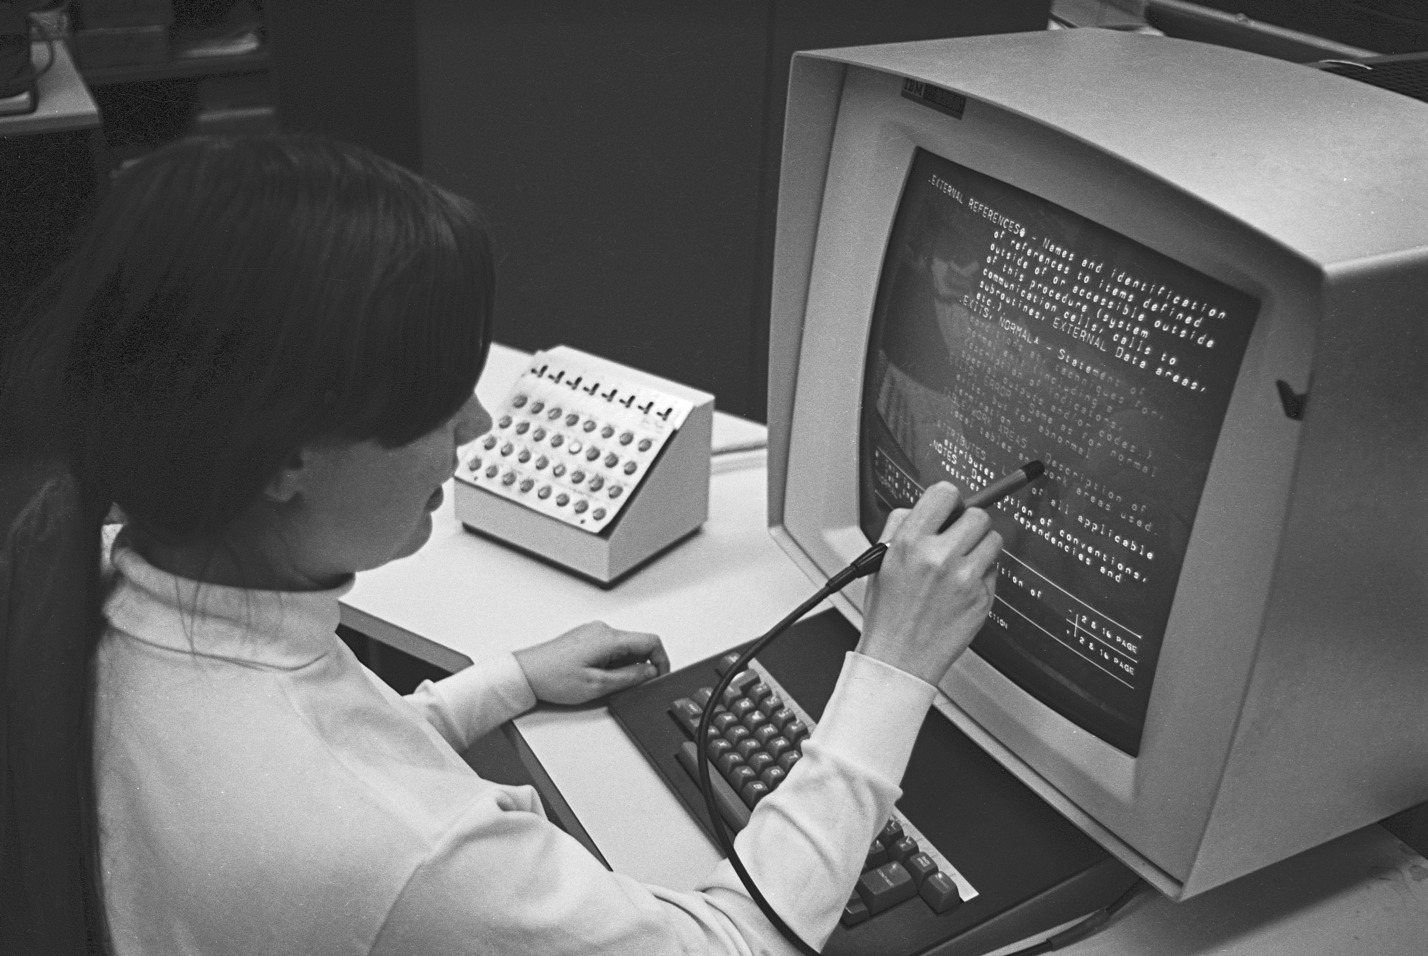
\includegraphics[width=0.75\textwidth]{im/hes.jpg}
\caption{A computer operator using the Hypertext Editing
System in 1969. (Gregory Lloyd from
\href{https://commons.wikimedia.org/wiki/File:HES_IBM_2250_Console_grlloyd_Oct1969.png}{Wikipedia},
\href{https://creativecommons.org/licenses/by-sa/4.0/deed.en}{CC BY-SA
4.0 International}.)}
\label{fig:HyperText}
\end{figure}
%\footnotetext{Gregory Lloyd from Wikipedia, CC BY-SA 4.0 International.}

%\end{center}

Independently of Project Xanadu, the first hyperlink system appeared for
scrolling within a single document; it was later generalized to linking
between multiple documents. And just like those original systems, the
web has linking within documents as well as between them. For example,
the URL \texttt{http://browser.engineering/history.html\#the-web-emerges}
refers to a document called ``\texttt{history.html}'', and specifically
to the element in it with the name ``\texttt{the-web-emerges}'': this
section. Visiting that URL will load this chapter and scroll to this
section.

This work also formed and inspired one of the key parts of Douglas
Engelbart's
\href{https://en.wikipedia.org/wiki/The_Mother_of_All_Demos}{mother of
all demos}, perhaps the most influential technology demonstration in the
history of computing (see Figure~\ref{fig:DougEnglebart}). That demo not only showcased the key concepts of
the web, but also introduced the computer mouse and graphical user
interface, both of which are of course central components of a browser
UI.\footnote{That demo went beyond even this. There are some parts of it
  that have not yet been realized in any computer system. Watch it!}

%\begin{center}

\begin{figure}[tbp]
\centering
\includegraphics[width=0.75\textwidth]{im/engelbart.jpg}
\caption{Doug Engelbart presenting the mother of all demos.
(SRI International, via the
\href{https://www.dougengelbart.org/content/view/374/464/}{Doug
Engelbart Institute}.)}
\label{fig:DougEnglebart}
\end{figure}
%\footnotetext{SRI International, via the Doug Engelbart Institute.}

%\end{center}

There is of course a very direct connection between this research and
the document--URL--hyperlink setup of the web, which built on the
hypertext idea and applied it in practice. The
\href{http://www.cs.umd.edu/hcil/hyperties/}{HyperTIES} system, for
example, had highlighted hyperlinks and was used to develop the world's
first electronically published academic journal, the 1988 issue of the
\href{https://cacm.acm.org/}{\textit{Communications of the ACM}}. Tim Berners-Lee
cites that 1988 issue as inspiration for the World Wide Web,\footnote{Nowadays
  the World Wide Web is called just ``the web'', or ``the web
  ecosystem''---ecosystem being another way to capture the same concept
  as ``World Wide''. The original wording lives on in the
  ``www''\index{WWW} in many website\index{website} domain names.} in
which he joined the link concept with the availability of the internet,
thus realizing many of the original goals of all this work from previous
decades.\footnote{Just as the web itself is a realization of previous
  ambitions and dreams, today we strive to realize the vision laid out
  by the web. (No, it's not done yet!)}

The word ``hyperlink'' may have been coined in 1987, in connection with
the \href{https://en.wikipedia.org/wiki/HyperCard}{HyperCard} system on
Apple computers. This system was also one of the first, or perhaps the
first, to introduce the concept of augmenting hypertext with
scripts\index{script} that handle user events like clicks and perform
actions that enhance the UI---just like JavaScript on a web page! It also
had graphical UI elements, not just text, unlike most predecessors.

In 1989--1990, the first web browser\index{web!browser} (named
WorldWideWeb, see Figure~\ref{fig:WorldWideWeb}) and web server (named \texttt{httpd}, for HTTP
Daemon, according to UNIX naming conventions) were born, written by Tim
Berners-Lee. Interestingly, while that browser's capabilities were in
some ways inferior to the browser you will implement in this
book,\footnote{No CSS! No JS! Not even images!} in other ways they go
beyond the capabilities available even in modern browsers.\footnote{For
  example, the first browser included the concept of an index page meant
  for searching within a site (vestiges of which exist today in the
  ``index.html'' convention when a URL path ends in /''), and had a
  WYSIWYG web page editor (the ``contenteditable'' HTML attribute and
  ``html()'' method on DOM elements (see Chapter~\ref{ch:DocumentTree}) have similar semantic behavior, but
  built-in file saving is gone). Today, the index is replaced with a
  search engine, and web page editors as a concept are somewhat obsolete
  due to the highly dynamic nature of today's web page rendering.} On
December~20, 1990 the
\href{http://info.cern.ch/hypertext/WWW/TheProject.html}{first web page}
was created. The browser we will implement in this book is easily able
to render this web page, even today.\footnote{Also, as you can see
  clearly, that web page has not been updated in the meantime, and
  retains its original aesthetics!} In 1991, Berners-Lee advertised his
browser and the concept on the
\href{https://www.w3.org/People/Berners-Lee/1991/08/art-6484.txt}{alt.hypertext
Usenet group}.

%\begin{center}

\begin{figure}[tbp]
\centering
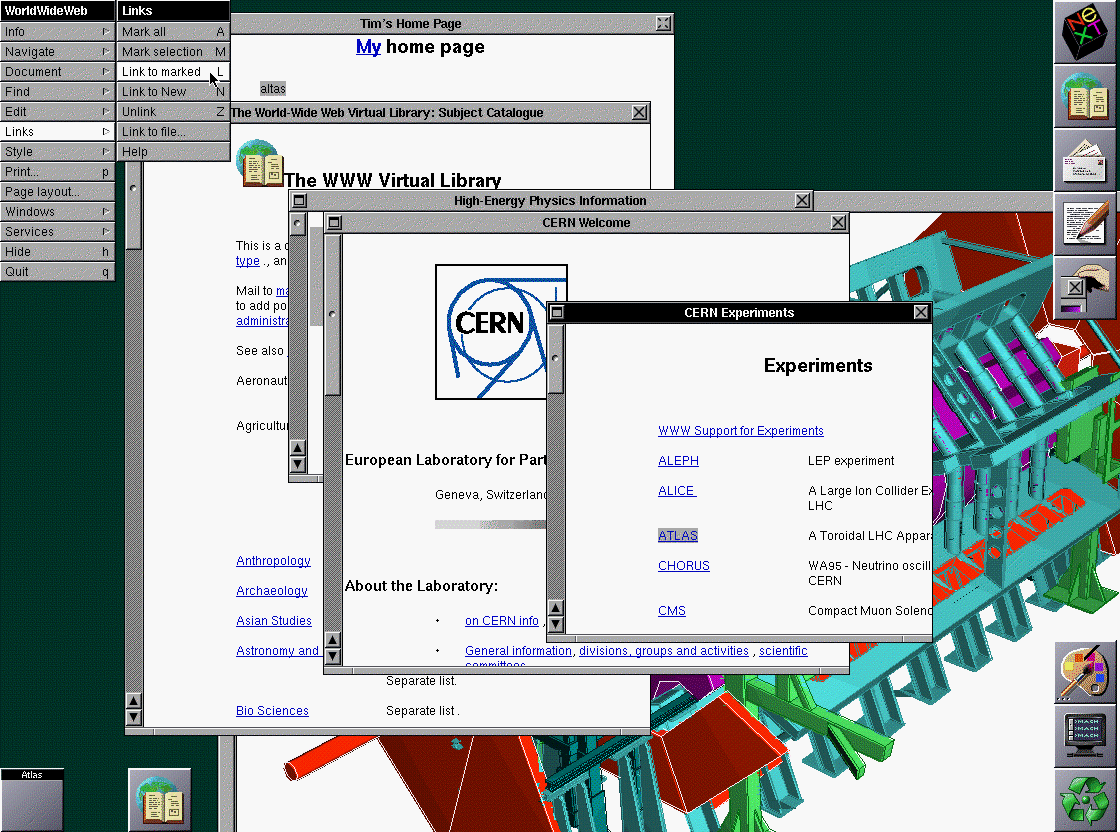
\includegraphics[width=0.75\textwidth]{im/worldwideweb.png}
\caption{Screenshot of the WorldWideWeb browser.
(\href{https://dl.acm.org/doi/10.1145/179606.179671}{\emph{Communications
of the ACM}}, August 1994.)}
\label{fig:WorldWideWeb}
\end{figure}
%\footnotetext{Communications of the ACM, August 1994.}

%\end{center}

Berners-Lee's
\href{https://www.w3.org/DesignIssues/TimBook-old/History.html}{Brief
History of the Web} highlights a number of other key factors that led to
the World Wide Web becoming the web we know today. One key factor was
its decentralized nature, which he describes as arising from the
academic culture of \href{https://home.cern/}{CERN}, where he worked.
The decentralized nature of the web is a key feature that distinguishes
it from many systems that came before or after, and his explanation of
it is worth quoting here (the italics are mine):
\begin{quote}
There was clearly a need for something like Enquire\footnote{Enquire was
  a predecessor web-like database system, also written by Berners-Lee.}
but accessible to everyone. I wanted it to scale so that if two people
started to use it independently, and later started to work together,
\emph{they could start linking together their information without making
any other changes}. This was the concept of the web.
\end{quote}

This quote captures one of the key value propositions of the web: its
decentralized nature. The web was successful for several reasons, but
they all had to do with decentralization:
\begin{itemize}
\item
  Because there was no gatekeeper to doing anything, it was easy for
  anyone, even novices, to make simple web pages and publish them.
\item
  Because pages were identified simply by URLs, traffic could come to
  the web from outside sources like email, social networking, and search
  engines. Further, compatibility between sites and the power of
  hyperlinks created
  \href{https://en.wikipedia.org/wiki/Network_effect}{network effects}
  that further strengthened the effect of hyperlinks from \emph{within}
  the web.
\item
  Because the web was outside the control of any one entity---and kept
  that way via standards organizations---it avoided the problems of
  monopoly control and manipulation.
\end{itemize}

\hypertarget{browsers}{%
\section{Browsers}\label{browsers}}

The first \emph{widely distributed} browser may have been
\href{https://en.wikipedia.org/wiki/ViolaWWW}{ViolaWWW} (see Figure~\ref{fig:ViolaWWW}); this browser
also pioneered multiple interesting features such as applets and images.
It was in turn the inspiration for
\href{https://en.wikipedia.org/wiki/Mosaic_(web_browser)}{NCSA Mosaic} (see Figure~\ref{fig:Mosaic}),
which launched in 1993. One of the two original authors of Mosaic went
on to co-found Netscape, which built
\href{https://en.wikipedia.org/wiki/Netscape_Navigator}{Netscape
Navigator} (see Figure~\ref{fig:NetscapeNavigator}), the first \emph{commercial browser},\footnote{By commercial
  I mean built by a for-profit entity. Netscape's early versions were
  also not free software---you had to buy them from a store. They cost
  about \$50.} which launched in 1994.
\href{https://lettersofnote.com/2011/07/22/the-internet-tidal-wave/}{Feeling
threatened}, Microsoft launched Internet Explorer (see Figure~\ref{fig:InternetExplorer}) in 1995 and soon
bundled it with Windows~95.

%\begin{center}

\begin{figure}[tbp]
\centering
\includegraphics[width=0.8\textwidth]{im/violawww.png}
\caption{ViolaWWW.
(\href{https://web.archive.org/web/20200706084621/http://viola.org/viola/book/preface.html}{\emph{Viola
in a Nutshell}.})}
\label{fig:ViolaWWW}
\end{figure}
%\footnotetext{Viola in a Nutshell}

%\end{center}

%\begin{center}

\begin{figure}[tbp]
\centering
\includegraphics[width=0.8\textwidth]{im/mosaic.png}
\caption{Mosaic.
(\href{https://commons.wikimedia.org/wiki/File:NCSA_Mosaic_Browser_Screenshot.png}{Wikipedia},
\href{https://creativecommons.org/publicdomain/zero/1.0/legalcode}{CC0
1.0}.)}
\label{fig:Mosaic}
\end{figure}
%\footnotetext{Wikipedia, CC0 1.0}

%\end{center}

%\begin{center}

\begin{figure}[tbp]
\centering
\includegraphics[width=0.8\textwidth]{im/netscape.png}
\caption{Netscape Navigator 1.22.
(\href{https://en.wikipedia.org/wiki/File:Navigator_1-22.png\#filehistory}{Wikipedia}.)}
\label{fig:NetscapeNavigator}
\end{figure}
%\footnotetext{Wikipedia}

%\end{center}

%\begin{center}

\begin{figure}[tbp]
\centering
\includegraphics[width=0.8\textwidth]{im/ie1.png}
\caption{Internet Explorer 1.0.
(\href{https://en.wikipedia.org/wiki/File:Internet_Explorer_1.0.png}{Wikipedia},
used with
\href{https://www.microsoft.com/en-us/legal/copyright/permissions}{permission
from Microsoft}.)}
\label{fig:InternetExplorer}
\end{figure}
%\footnotetext{Wikipedia, used with permission from Microsoft}

%\end{center}

The era of the
\href{https://en.wikipedia.org/wiki/Browser_wars\#First_Browser_War_(1995\%E2\%80\%932001)}{``first
browser war''} ensued: a competition between Netscape Navigator and
\href{https://en.wikipedia.org/wiki/Internet_Explorer}{Internet
Explorer}. There were also other browsers with smaller market shares;
one notable example is
\href{https://en.wikipedia.org/wiki/Opera_(web_browser)}{Opera}. The
\href{https://en.wikipedia.org/wiki/WebKit}{WebKit} project began in
1999; \href{https://en.wikipedia.org/wiki/Safari_(web_browser)}{Safari}
and \href{https://www.chromium.org/}{Chromium}-based browsers, such as
Chrome and newer versions of
\href{https://en.wikipedia.org/wiki/Microsoft_Edge}{Edge}, descend from
this codebase. Likewise, the
\href{https://en.wikipedia.org/wiki/Gecko_(software)}{Gecko} rendering
engine\index{rendering!engine} was originally developed by Netscape
starting in 1997; the
\href{https://en.wikipedia.org/wiki/Firefox}{Firefox} browser is
descended from that codebase. During the first browser war, nearly all
of the core features of this book's simple browser were added, including
CSS, DOM, and JavaScript.

The ``second browser war'', which according to Wikipedia was
\href{https://en.wikipedia.org/wiki/Browser_wars\#Second_Browser_War_(2004\%E2\%80\%932017)}{2004--2017},
was fought between a variety of browsers, in particular Internet
Explorer, Firefox, Safari, and Chrome. Initially, Safari and Chrome used
the same rendering engine, but Chrome forked into
\href{https://en.wikipedia.org/wiki/Blink_(browser_engine)}{Blink} in
2013, which Microsoft Edge adopted by 2020. The second browser war saw
the development of many features of the modern web, including widespread
use of AJAX\footnote{Asynchronous JavaScript and XML, where XML stands for eXtensible Markup Language.}
requests, HTML5 features like
\texttt{\textless{}canvas\textgreater{}}, and a huge explosion in
third-party JavaScript libraries and frameworks.

\hypertarget{web-standards}{%
\section{Web Standards}\label{web-standards}}

In parallel with these developments was another, equally important,
one---the standardization of web APIs. In October 1994, the
\href{https://www.w3.org/Consortium/facts}{World Wide Web Consortium}
(W3C)\index{W3C} was founded to provide oversight and standards for web
features. Prior to this point, browsers would often introduce new HTML
elements or APIs, and competing browsers would have to copy them. With a
standards organization, those elements and APIs could subsequently be
agreed upon and documented in specifications. (These days, an initial
discussion, design, and specification precedes any new feature.) Later
on, the HTML specification ended up moving to a different standards body
called the \href{https://whatwg.org/}{WHATWG}\index{WHATWG}, but
\href{https://drafts.csswg.org/}{CSS} and other features are still
standardized at the W3C. JavaScript\index{JavaScript} is standardized at
\href{https://tc39.es/}{TC39}\index{TC39} (``Technical Committee 39'' at
\href{https://www.ecma-international.org/about-ecma/history/}{ECMA}, yet
another standards body).
\href{https://tools.ietf.org/html/rfc2616}{HTTP} is standardized by the
\href{https://www.ietf.org/about/}{IETF}\index{IETF}. The point is that
the standards process set up in the mid-1990s is still with us.

In the first years of the web, it was not so clear that browsers would
remain standard and that one browser might not end up ``winning'' and
becoming another proprietary software platform. There are multiple
reasons this didn't happen, among them the egalitarian ethos of the
computing community and the presence and strength of the W3C. Another
important reason was the networked nature of the web, and therefore the
necessity for web developers to make sure their pages worked correctly
in most or all of the browsers (otherwise they would lose customers),
leading them to avoid proprietary extensions. On the contrary, browsers
worked hard to carefully reproduce each other's undocumented
behaviors---even bugs---to make sure they continued supporting the whole
web.

There never really was a point where any browser openly attempted to
break away from the standard, despite fears that that might
happen.\footnote{Perhaps the closest the web came to fragmenting was
  with the late-1990s introduction of features for
  \href{https://en.wikipedia.org/wiki/Dynamic_HTML}{DHTML}---early
  versions of the Document Object Model you'll learn about in this book.
  Netscape and Internet Explorer at first had incompatible
  implementations of these features, and it took years, the development of a
  common specification, and significant pressure campaigns on the
  browsers before standardization was achieved. You can read about this
  story in much more depth
  \href{https://css-tricks.com/chapter-7-standards/}{here}.} Instead,
intense competition for market share was channeled into very fast
innovation and an ever-expanding set of APIs and capabilities for the
web, which we nowadays refer to as \emph{the web platform}, not just the
``World Wide Web''. This recognizes the fact that the web is no longer a
document viewing mechanism, but has evolved into a fully realized
computing platform and ecosystem.\footnote{There have even been
  operating systems built around the web! Examples include
  \href{https://en.wikipedia.org/wiki/WebOS}{webOS}, which powered some
  Palm smartphones,
  \href{https://en.wikipedia.org/wiki/Firefox_OS}{Firefox OS} (that
  today lives on in
  \href{https://en.wikipedia.org/wiki/KaiOS}{KaiOS}-based phones), and
  \href{https://en.wikipedia.org/wiki/Chrome_OS}{ChromeOS}, which is a
  desktop operating system. All of these operating systems are based on using the web
  as the UI layer for all applications, with some JavaScript-exposed
  APIs on top for system integration.}

Given the outcomes---multiple competing browsers and well-developed
standards---it is in retrospect not that relevant which browser ``won''
or ``lost'' each of the browser ``wars''. In each case \emph{the web}
won, because it gained users and grew in capability.

\hypertarget{open-source}{%
\section{Open Source}\label{open-source}}

Another important and interesting outcome of the \emph{second} browser
war was that all mainstream browsers today\footnote{Examples of
  Chromium-based browsers include Chrome, Edge, Opera (which switched to
  Chromium from the
  \href{https://en.wikipedia.org/wiki/Presto_(browser_engine)}{Presto}
  engine in 2013), Samsung Internet, Yandex Browser, UC Browser, and
  Brave. In addition, there are many ``embedded'' browsers, based on one
  or another of the three engines, for a wide variety of automobiles,
  phones, TVs, and other electronic devices.} are based on \emph{three
open-source web rendering~/ JavaScript\index{JavaScript} engines}:
Chromium, Gecko, and WebKit.\footnote{The JavaScript engines are actually
  in different repositories (as are various other subcomponents), and
  can and do get used outside the browser as JavaScript virtual
  machines. One important application is the use of
  \href{https://en.wikipedia.org/wiki/V8_(JavaScript_engine)}{V8} to
  power \href{https://en.wikipedia.org/wiki/Node.js}{node.js}. However,
  each of the three rendering engines does have a corresponding
  JavaScript implementation, so conflating the two is reasonable.} Since
Chromium and WebKit have a common ancestral codebase, while Gecko is an
open-source descendant of Netscape, all three date back to the
1990s---almost to the beginning of the web.

This is not an accident, and in fact tells us something quite
interesting about the most cost-effective way to implement a rendering
engine based on a commodity set of platform APIs. For example, it's
common for independent developers, not paid by the company nominally
controlling the browser, to contribute code and features. There are even
companies and individuals that specialize in implementing browser
features! It's also common for features in one browser to copy code from
another. And every major browser being open source feeds back into the
standards process, reinforcing the web's decentralized nature.

\hypertarget{summary}{%
\section{Summary}\label{HistoryOfTheWeb-summary}}

In summary, the history went like this:
\begin{enumerate}[label=\arabic*.]
%\def\labelenumi{\arabic{enumi}.}
\item
  Basic research was performed into % the
  ways to represent and explore information.
\item
  Once the necessary technology became mature enough, the web proper was
  proposed and implemented.
\item
  The web became popular quite quickly, and many browsers appeared in
  order to capitalize on the web's opportunity.
\item
  Standards organizations were introduced in order to negotiate between
  the browsers and avoid proprietary control.
\item
  Competition between browsers grew their power and complexity at a
  rapid pace.
\item
  Browsers appeared on all devices and operating systems, from desktop
  to mobile to embedded.
\item
  Eventually, all web rendering engines became open source, as a
  recognition of their being a shared effort larger than any single
  entity.
\end{enumerate}
The web has come a long way! But one thing seems clear: it isn't done
yet.

\hypertarget{exercises}{%
\section{Exercises}\label{HistoryOfTheWeb-exercises}}
\begin{enumerate}[label=\thechapter-\arabic*]
\item \emph{What comes next?} Based on what you learned about how the web came
about and took its current form, what trends do you predict for its
future evolution? For example, do you think it'll compete effectively
against other non-web technologies and platforms?

\item \emph{What became of the original ideas?} The way the web works in
practice is significantly different than the memex; one key difference
is that there is no built-in way for the \emph{user} of the web to add
links between pages or notate them. Why do you think this is? Can you
think of other goals from the original work that remain unrealized?
\end{enumerate}

\ifprintedoutput
\theendnotes
\setcounter{endnote}{0}
\fi

\part{Drawing Graphics}

 % EDIT: number body sections
\renewcommand\thechapter{\arabic{chapter}}
\setcounter{chapter}{0} % EDIT: Reset chapter numbering

\chapter{Downloading Web Pages}\label{ch:DownloadingWebPages}
A web browser displays information identified by a URL. And the first
step is to use that URL to connect to and download that information from
a server somewhere on the Internet.

\hypertarget{connecting-to-a-server}{%
\section{Connecting to a Server}\label{connecting-to-a-server}}

Browsing the internet starts with a URL\index{URL},\footnote{``URL''
  stands for ``uniform resource locator'', meaning that it is a portable
  (uniform) way to identify web pages (resources\index{web!resource})
  and also that it describes how to access those files (locator).} a
short string that identifies a particular web page that the browser
should visit. % A URL looks like this:

% This
A URL has three parts (see Figure~\ref{fig:URLsyntax}): the scheme\index{scheme} explains \emph{how}
to get the information; the host name explains \emph{where} to get it; and
the path\index{path} explains \emph{what} information to get. There are
also optional parts to the URL, like ports, queries, and fragments,
which we'll see later.

\begin{figure}[btp]
\centering
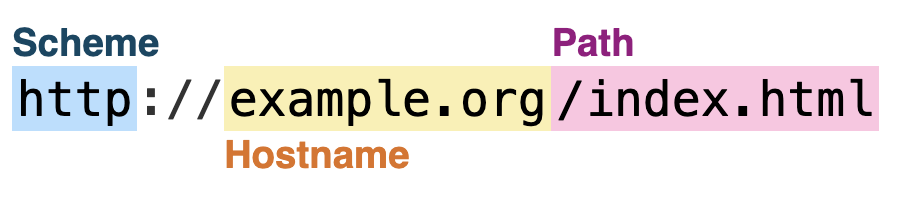
\includegraphics[width=0.7\textwidth]{im/http-url.png}
\caption{The syntax of URLs.}\label{fig:URLsyntax}
\end{figure}

From a URL, the browser can start the process of downloading the web
page. The browser first asks the local operating system (OS) to put it in touch with the
\emph{server} described by the \emph{host name}. The OS then talks to a
\emph{DNS} (Domain Name System) server which converts\footnote{You can use a DNS lookup tool
  like \href{https://nslookup.io}{nslookup.io} or the \texttt{dig}
  command to do this conversion yourself.} a host name like
\texttt{example.org} into a \emph{destination IP address} like
\texttt{93.184.216.34}.\footnote{Today there are two versions of IP (Internet Protocol):
  IPv4 and IPv6. IPv6 addresses are a lot longer and are usually written in hexadecimal,
  but otherwise the differences don't matter here.} Then the OS decides
which hardware is best for communicating with that destination IP
address (say, wireless or wired) using what is called a \emph{routing
table}, and then uses device drivers to send signals over a wire or over
the air.\footnote{I'm skipping steps here. On wires you first have to
  wrap communications in ethernet frames, on wireless you have to do
  even more. I'm trying to be brief.} Those signals are picked up and
transmitted by a series of \emph{routers}\footnote{Or a switch, or an
  access point; there are a lot of possibilities, but eventually there
  is a router.} which each choose the best direction to send your
message so that it eventually gets to the destination.\footnote{They may
  also record where the message came from so they can forward the reply
  back.} %, especially in the case of NATs.}
When the message reaches the
server, a connection is created. Anyway, the point of this is that the
browser tells the OS, ``Hey, put me in touch with
\texttt{example.org}'', and it does.

On many systems, you can set up this kind of connection using the
\texttt{telnet} program, like this:\footnote{The ``80'' is the port,
  discussed below.}
\begin{bookblock*}{notcode}
\begin{Shaded}
\begin{Highlighting}[]
\NormalTok{telnet example.org 80}
\end{Highlighting}
\end{Shaded}
\end{bookblock*}
\noindent (Note: When you see a % gray outline
black frame, it means that the code in question
is an example only, and \emph{not} actually part of our browser's code.)

\begin{bookblock}{installation}
You might need to install \texttt{telnet}; it is often disabled by
default. On Windows,
\href{https://www.lifewire.com/what-is-telnet-2626026}{go to Programs
and Features / Turn Windows features on or off} in the Control Panel;
you'll need to reboot. When you run it, it'll clear the screen instead
of printing something, but other than that works normally. On macOS, you
can use the \texttt{nc\ -v} command as a replacement for
\texttt{telnet}:
\begin{bookblock*}{notcode}
\begin{Shaded}
\begin{Highlighting}[]
\NormalTok{nc {-}v example.org 80}
\end{Highlighting}
\end{Shaded}
\end{bookblock*}
The output is a little different but it works in the same way. On most
Linux systems, you can install \texttt{telnet} or \texttt{nc} from the
package manager, usually from packages called \texttt{telnet} and
\texttt{netcat}.
\end{bookblock}

You'll get output that looks like this:
\begin{verbatim}
Trying 93.184.216.34...
Connected to example.org.
Escape character is '^]'.
\end{verbatim}
This means that the OS converted the host name \texttt{example.org} into
the IP address \texttt{93.184.216.34} and was able to connect to
it.\footnote{The line about escape characters is just instructions on
  using obscure \texttt{telnet} features.} You can now talk to
\texttt{example.org}.

\begin{bookblock}{further}
The URL syntax is defined in
\href{https://tools.ietf.org/html/rfc3986}{RFC~3987}, whose first author
is Tim Berners-Lee---no surprise there! The second author is Roy
Fielding, a key contributor to the design of HTTP and also well known
for describing the Representational State Transfer (REST) architecture of the web in his
\href{https://ics.uci.edu/~fielding/pubs/dissertation/fielding_dissertation_2up.pdf}{Ph.D.\ thesis},
which explains how REST allowed the web to grow in a
decentralized way. Today, many services provide ``RESTful APIs'' that
also follow these principles, though there does seem to be
\href{https://twobithistory.org/2020/06/28/rest.html}{some confusion}
about it.
\end{bookblock}

\hypertarget{requesting-information}{%
\section{Requesting Information}\label{requesting-information}}

Once it's connected, the browser requests information from the server by
giving its \emph{path}, the path being the part of a URL that comes
after the host name, like \texttt{/index.html}. The structure of the request
is shown in Figure~\ref{fig:HttpGet}. %looks like this;
You can type % it
this into \texttt{telnet} to try it.
% (make sure to type a blank line after the \texttt{Host} line).

\begin{figure}[b!]
\centering
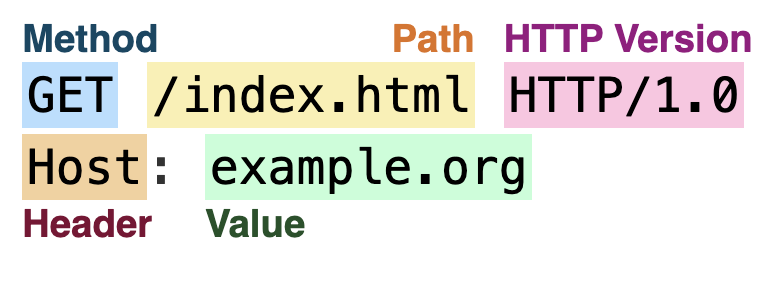
\includegraphics[width=0.7\textwidth]{im/http-get.png}
\caption{An annotated HTTP GET request.}\label{fig:HttpGet}
\end{figure}

Here, the word \texttt{GET}\index{GET} means that the browser would like
to receive information,\footnote{It could say \texttt{POST} if it
  intended to send information, plus there are some other, more obscure,
  options.} then comes the path, and finally there is the word
\texttt{HTTP/1.0} which tells the host that the browser speaks version
1.0 of
\href{https://developer.mozilla.org/en-US/docs/Web/HTTP}{HTTP}\index{HTTP}.
There are several versions of HTTP
(\href{https://medium.com/platform-engineer/evolution-of-http-69cfe6531ba0}{0.9,
1.0, 1.1, 2.0, and 3.0}). The HTTP~1.1 standard adds a variety of useful
features, like keep-alive, but in the interest of simplicity our browser
won't use them. We're also not implementing HTTP~2.0; % HTTP 2.0
it is much
more complex than the 1.$x$ series, and is intended for large and complex
web applications, which our browser can't run anyway.

After the first line, each line contains a \emph{header}, which has a
name (like \texttt{Host}) and a value (like \texttt{example.org}).
Different headers mean different things; the \texttt{Host} header, for
example, tells the server who you think it is.\footnote{This is useful
  when the same IP address corresponds to multiple host names and hosts
  multiple websites (for example, \texttt{example.com} and
  \texttt{example.org}). The \texttt{Host} header tells the server which
  of multiple websites you want. These websites basically require the
  \texttt{Host} header to function properly. Hosting multiple domains on
  a single computer is very common.} There are lots of other headers one
could send, but let's stick to just \texttt{Host} for now.

Finally, after the headers comes a single blank line; that tells the
host that you are done with headers. So type a blank line into
\texttt{telnet} (hit Enter twice after typing the two lines of the request) % above)
and you should get a response from \texttt{example.org}.

\begin{bookblock}{further}
HTTP/1.0 is standardized in
\href{https://tools.ietf.org/html/rfc1945}{RFC~1945}, and HTTP/1.1 in
\href{https://tools.ietf.org/html/rfc2616}{RFC~2616}. HTTP was designed
to be simple to understand and implement, making it easy for any kind of
computer to adopt it. It's no coincidence that you can type HTTP
directly into \texttt{telnet}! Nor is it an accident that HTTP is a
``line-based protocol'', using plain text and newlines, similar to
the Simple Mail Transfer Protocol
(\href{https://en.wikipedia.org/wiki/Simple_Mail_Transfer_Protocol}{SMTP})
for email. Ultimately, the whole pattern derives from early computers
only having line-based text input. In fact, one of the first two
browsers had a
\href{https://en.wikipedia.org/wiki/Line_Mode_Browser}{line-mode UI}.
\end{bookblock}

\hypertarget{the-servers-response}{%
\section{The Server's Response}\label{the-servers-response}}

The server's response starts with % this
the line in Figure~\ref{fig:HttpResponse1}.
\begin{figure}[b!]
\centering
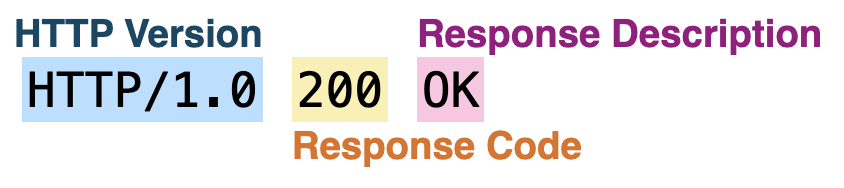
\includegraphics[width=0.7\textwidth]{im/http-status.png}
\caption{Annotated first line of an HTTP response.}\label{fig:HttpResponse1}
\end{figure}
This tells you that the host confirms that it, too, speaks
\texttt{HTTP/1.0}, and that it found your request to be ``OK'' (which
has a numeric code of 200). You may be familiar with
\texttt{404\ Not\ Found}; that's another numeric code and response, as
are \texttt{403\ Forbidden} or \texttt{500\ Server\ Error}. There are
lots of these codes,\footnote{As % any look at a
  \href{https://github.com/for-GET/http-decision-diagram}{this flow chart} % will
  shows.} and they have a pretty neat organization
scheme:\footnote{The status text like \texttt{OK} can actually be
  anything and is just there for humans, not for machines.}
\begin{itemize}
\tightlist
\item
  the 100s are informational messages;
\item
  the 200s mean you were successful;
\item
  the 300s request follow-up action (usually a redirect);
\item
  the 400s mean you sent a bad request;
\item
  the 500s mean the server handled the request badly.
\end{itemize}
Note the genius of having two sets of error codes (400s and 500s) %, which
to tell you who is at fault, the server or the browser.\footnote{More
  precisely, who the server thinks is at fault.} You can find a full
list of the different codes
\href{https://en.wikipedia.org/wiki/List_of_HTTP_status_codes}{on
Wikipedia}, and new ones do get added here and there.

After the \texttt{200\ OK} line, the server sends its own headers. When
I did this, I got these headers (but yours will differ):
\begin{bookblock*}{notcode}
\begin{Shaded}
\begin{Highlighting}[]
\NormalTok{Age: 545933}
\NormalTok{Cache{-}Control: max{-}age=604800}
\NormalTok{Content{-}Type: text/html; charset=UTF{-}8}
\NormalTok{Date: Mon, 25 Feb 2019 16:49:28 GMT}
\NormalTok{Etag: "1541025663+gzip+ident"}
\NormalTok{Expires: Mon, 04 Mar 2019 16:49:28 GMT}
\NormalTok{Last{-}Modified: Fri, 09 Aug 2013 23:54:35 GMT}
\NormalTok{Server: ECS (sec/96EC)}
\NormalTok{Vary: Accept{-}Encoding}
\NormalTok{X{-}Cache: HIT}
\NormalTok{Content{-}Length: 1270}
\NormalTok{Connection: close}
\end{Highlighting}
\end{Shaded}
\end{bookblock*}
\noindent There is \emph{a lot} here, about the information you are requesting
(\texttt{Content-Type}, \texttt{Content-Length}, and
\texttt{Last-Modified}), about the server (\texttt{Server},
\texttt{X-Cache}), about how long the browser should cache this
information (\texttt{Cache-Control}, \texttt{Expires}, \texttt{Etag}),
and about all sorts of other stuff. Let's move on for now.

After the headers there is a blank line followed by a bunch of
\href{https://developer.mozilla.org/en-US/docs/Web/HTML}{HTML}\index{HTML}
code. This is called the \emph{body} of the server's response, and your
browser knows that it is HTML because of the \texttt{Content-Type}
header, which says that it is \texttt{text/html}. It's this HTML code
that contains the content of the web page itself.

The HTTP request/response transaction is summarized in Figure~\ref{fig:HttpRequestResponse}.
Let's now switch gears from manual connections to Python.

\begin{figure}
\centering
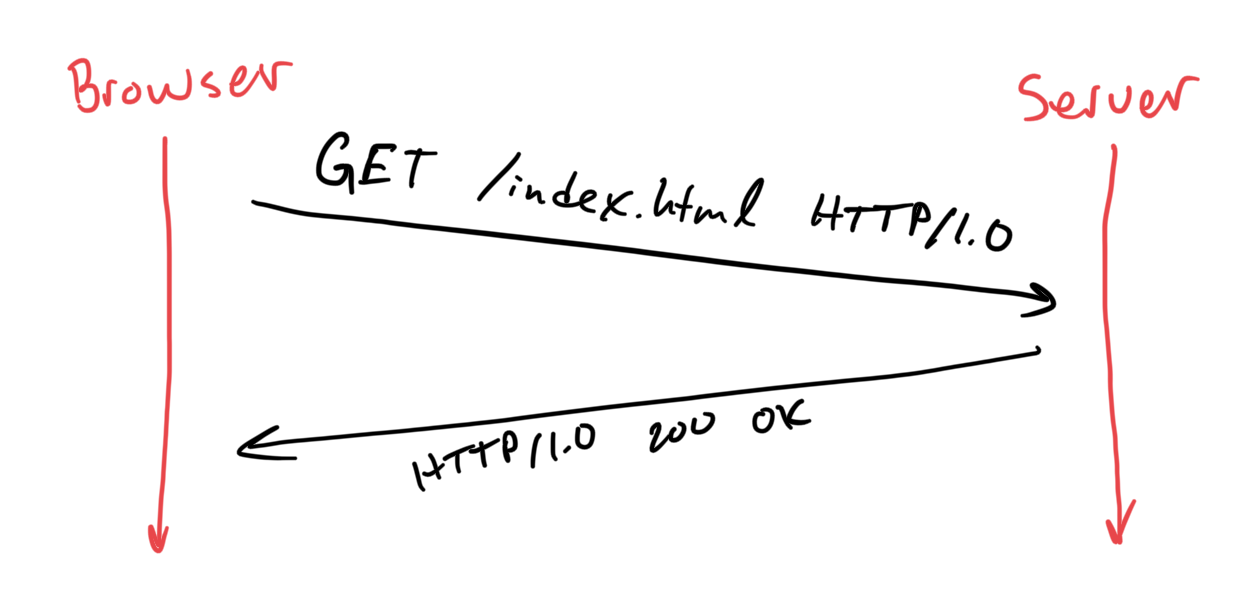
\includegraphics{im/http-request.png}
\caption{An HTTP request and response pair are how a web browser gets
web pages from a web server.}\label{fig:HttpRequestResponse}
\end{figure}

\begin{bookblock}{further}
Wikipedia has nice lists of HTTP
\href{https://en.wikipedia.org/wiki/List_of_HTTP_header_fields}{headers}
and
\href{https://en.wikipedia.org/wiki/List_of_HTTP_status_codes}{response
codes}. Some of the HTTP response codes are almost never used, like
\href{https://developer.mozilla.org/en-US/docs/Web/HTTP/Status/402}{402}
``Payment Required''. This code was intended to be used for ``digital
cash or (micro) payment systems''. While e-commerce is alive and well
without the response code 402,
\href{https://en.wikipedia.org/wiki/Micropayment}{micropayments} have
not (yet?) gained much traction, even though many people (including me!)
think they are a good idea.
\end{bookblock}

\hypertarget{telnet-in-python}{%
\section{Telnet in Python}\label{telnet-in-python}}

So far we've communicated with another computer using \texttt{telnet}.
But it turns out that \texttt{telnet} is quite a simple program, and we
can do the same programmatically. It'll require extracting the host name and
path from the URL, creating a \emph{socket}, sending a request, and
receiving a response.\footnote{In Python, there's a library called
  \texttt{urllib.parse} for parsing URLs, but I think implementing our
  own will be good for learning. Plus, it makes this book less
  Python-specific.}

Let's start with parsing the URL. I'm going to make parsing a URL return
a \texttt{URL} object, and I'll put the parsing code into the
constructor:
\begin{Shaded}
\begin{Highlighting}[]
\KeywordTok{class}\NormalTok{ URL:}
    \KeywordTok{def} \FunctionTok{\_\_init\_\_}\NormalTok{(}\VariableTok{self}\NormalTok{, url):}
        \CommentTok{\# ...}
\end{Highlighting}
\end{Shaded}
The \texttt{\_\_init\_\_} method is Python's peculiar syntax for class
constructors, and the \texttt{self} parameter, which you must always
make the first parameter of any method, is Python's analog of
\texttt{this}.

Let's start with the scheme, which is separated from the rest of the URL
by \texttt{://}. Our browser only supports \texttt{http}, so I check
that, too:
\begin{Shaded}
\begin{Highlighting}[]
\KeywordTok{class}\NormalTok{ URL:}
    \KeywordTok{def} \FunctionTok{\_\_init\_\_}\NormalTok{(}\VariableTok{self}\NormalTok{, url):}
        \VariableTok{self}\NormalTok{.scheme, url }\OperatorTok{=}\NormalTok{ url.split(}\StringTok{"://"}\NormalTok{, }\DecValTok{1}\NormalTok{)}
        \ControlFlowTok{assert} \VariableTok{self}\NormalTok{.scheme }\OperatorTok{==} \StringTok{"http"}
\end{Highlighting}
\end{Shaded}

Now we must separate the host from the path. The host comes before the
first \texttt{/}, while the path is that slash and everything after it.
Let's add a function that parses all parts of a URL:
\begin{Shaded}
\begin{Highlighting}[]
\KeywordTok{class}\NormalTok{ URL:}
    \KeywordTok{def} \FunctionTok{\_\_init\_\_}\NormalTok{(}\VariableTok{self}\NormalTok{, url):}
        \CommentTok{\# ...}
        \ControlFlowTok{if} \StringTok{"/"} \KeywordTok{not} \KeywordTok{in}\NormalTok{ url:}
\NormalTok{            url }\OperatorTok{=}\NormalTok{ url }\OperatorTok{+} \StringTok{"/"}
        \VariableTok{self}\NormalTok{.host, url }\OperatorTok{=}\NormalTok{ url.split(}\StringTok{"/"}\NormalTok{, }\DecValTok{1}\NormalTok{)}
        \VariableTok{self}\NormalTok{.path }\OperatorTok{=} \StringTok{"/"} \OperatorTok{+}\NormalTok{ url}
\end{Highlighting}
\end{Shaded}
(When you see a code block with a \texttt{\#\ ...}, like this one, that
means you're adding code to an existing method or block.) The
\texttt{split(s,\ n)} method splits a string at the first \texttt{n}
copies of \texttt{s}. Note that there's some tricky logic here for
handling the slash between the host name and the path. That (optional)
slash is part of the path.

Now that the \texttt{URL} has the \texttt{host} and \texttt{path}
fields, we can download the web page at that URL. We'll do that in a new
method, \texttt{request}:
\begin{Shaded}
\begin{Highlighting}[]
\KeywordTok{class}\NormalTok{ URL:}
    \KeywordTok{def}\NormalTok{ request(}\VariableTok{self}\NormalTok{):}
        \CommentTok{\# ...}
\end{Highlighting}
\end{Shaded}
Note that you always need to write the \texttt{self} parameter for
methods in Python. In the future, I won't always make such a big deal
out of defining a method---if you see a code block with code in a method
or function that doesn't exist yet, that means we're defining it.

The first step to downloading a web page is connecting to the host. The
operating system provides a feature called ``sockets'' for this. When
you want to talk to other computers (either to tell them something, or
to wait for them to tell you something), you create a socket, and then
that socket can be used to send information back and forth. Sockets come
in a few different kinds, because there are multiple ways to talk to
other computers:
\begin{itemize}
%\tightlist
\item
  A socket has an \emph{address family}, which tells you how to find the
  other computer. Address families have names that begin with
  \texttt{AF}. We want \texttt{AF\_INET}, but for example
  \texttt{AF\_BLUETOOTH} is another.
\item
  A socket has a \emph{type}, which describes the sort of conversation
  that's going to happen. Types have names that begin with
  \texttt{SOCK}. We want \texttt{SOCK\_STREAM}, which means each
  computer can send arbitrary amounts of data, but there's also
  \texttt{SOCK\_DGRAM}, in which case they send each other packets of
  some fixed size.\footnote{\texttt{DGRAM} stands for ``datagram'',
    which I imagine to be like a postcard.}
\item
  A socket has a \emph{protocol}, which describes the steps by which the
  two computers will establish a connection. Protocols have names that
  depend on the address family, but we want
  \texttt{IPPROTO\_TCP}.\footnote{Newer versions of HTTP use something
    called \href{https://en.wikipedia.org/wiki/QUIC}{QUIC} instead of
    the Transmission Control Protocol (TCP), but our browser will stick to HTTP~1.0.}
\end{itemize}

By picking all of these options, we can create a socket like
so:\footnote{While this code uses the Python \texttt{socket} library,
  your favorite language likely contains a very similar library; the API
  is basically standardized. In Python, the flags we pass are defaults,
  so you can actually call \texttt{socket.socket()}; I'm keeping the
  flags here in case you're following along in another language.}
\begin{Shaded}
\begin{Highlighting}[]
\ImportTok{import}\NormalTok{ socket}

\KeywordTok{class}\NormalTok{ URL:}
    \KeywordTok{def}\NormalTok{ request(}\VariableTok{self}\NormalTok{):}
\NormalTok{        s }\OperatorTok{=}\NormalTok{ socket.socket(}
\NormalTok{            family}\OperatorTok{=}\NormalTok{socket.AF\_INET,}
            \NormalTok{type}\OperatorTok{=}\NormalTok{socket.SOCK\_STREAM,}
\NormalTok{            proto}\OperatorTok{=}\NormalTok{socket.IPPROTO\_TCP,}
\NormalTok{        )}
\end{Highlighting}
\end{Shaded}

Once you have a socket, you need to tell it to connect to the other
computer. For that, you need the host and a \emph{port}.\index{port} The
port depends on the protocol you are using; for now it should be 80.
\begin{Shaded}
\begin{Highlighting}[]
\KeywordTok{class}\NormalTok{ URL:}
    \KeywordTok{def}\NormalTok{ request(}\VariableTok{self}\NormalTok{):}
        \CommentTok{\# ...}
\NormalTok{        s.}\ExtensionTok{connect}\NormalTok{((}\VariableTok{self}\NormalTok{.host, }\DecValTok{80}\NormalTok{))}
\end{Highlighting}
\end{Shaded}
This talks to \texttt{example.org} to set up the connection and ready
both computers to exchange data.

\begin{bookblock}{quirk}
Naturally this won't work if you're offline. It also might not work if
you're behind a proxy, or in a variety of more complex networking
environments. The workaround will depend on your setup---it might be as
simple as disabling your proxy, or it could be much more complex.
\end{bookblock}

Note that there are two parentheses in the \texttt{connect} call:
\texttt{connect} takes a single argument, and that argument is a pair of
a host and a port. This is because different address families have
different numbers of arguments.

\begin{bookblock}{further}
The ``sockets'' API, which Python more or less implements directly,
derives from the original
``\href{https://en.wikipedia.org/wiki/Berkeley_sockets}{Berkeley
sockets}'' API design for 4.2 BSD Unix in 1983. Of course, Windows and
Linux merely reimplement the API, but macOS and iOS actually do
\href{https://developer.apple.com/library/archive/documentation/Darwin/Conceptual/KernelProgramming/BSD/BSD.html}{still
use} large amounts of code descended from BSD Unix.
\end{bookblock}

\hypertarget{request-and-response}{%
\section{Request and Response}\label{request-and-response}}

Now that we have a connection, we make a request to the other server. To
do so, we send it some data using the \texttt{send} method:
\begin{Shaded}
\begin{Highlighting}[]
\KeywordTok{class}\NormalTok{ URL:}
    \KeywordTok{def}\NormalTok{ request(}\VariableTok{self}\NormalTok{):}
        \CommentTok{\# ...}
\NormalTok{        request }\OperatorTok{=} \StringTok{"GET }\SpecialCharTok{\{\}}\StringTok{ HTTP/1.0}\CharTok{\textbackslash{}r\textbackslash{}n}\StringTok{"}\NormalTok{.}\BuiltInTok{format}\NormalTok{(}\VariableTok{self}\NormalTok{.path)}
\NormalTok{        request }\OperatorTok{+=} \StringTok{"Host: }\SpecialCharTok{\{\}}\CharTok{\textbackslash{}r\textbackslash{}n}\StringTok{"}\NormalTok{.}\BuiltInTok{format}\NormalTok{(}\VariableTok{self}\NormalTok{.host)}
\NormalTok{        request }\OperatorTok{+=} \StringTok{"}\CharTok{\textbackslash{}r\textbackslash{}n}\StringTok{"}
\NormalTok{        s.send(request.encode(}\StringTok{"utf8"}\NormalTok{))}
\end{Highlighting}
\end{Shaded}
The \texttt{send} method just sends the request to the
server.\footnote{\texttt{send} actually returns a number, in this case
  \texttt{47}. That tells you how many bytes of data you sent to the
  other computer; if, say, your network connection failed midway through
  sending the data, you might want to know how much you sent before the
  connection failed.} There are a few things in this code that have to
be exactly right. First, it's very important to use
\texttt{\textbackslash{}r\textbackslash{}n} instead of
\texttt{\textbackslash{}n} for newlines. It's also essential that you
put \emph{two} newlines \texttt{\textbackslash{}r\textbackslash{}n} at
the end, so that you send that blank line at the end of the request. If
you forget that, the other computer will keep waiting on you to send
that newline, and you'll keep waiting on its response.\footnote{Computers
  are endlessly literal-minded.}

Also note the \texttt{encode} call. When you send data, it's important
to remember that you are sending raw bits and bytes; they could form
text or an image or video. But a Python string is specifically for
representing text. The \texttt{encode} method converts text into bytes,
and there's a corresponding \texttt{decode} method that goes the other
way.\footnote{When you call \texttt{encode} and \texttt{decode} you need
  to tell the computer what \emph{character encoding} you want it to
  use. This is a complicated topic. I'm using \texttt{utf8} here, which
  is a common character encoding and will work on many pages, but in the
  real world you would need to be more careful.} Python reminds you to
be careful by giving different types to text and to bytes:
\begin{bookblock*}{notcode}
\begin{Shaded}
\begin{Highlighting}[]
\OperatorTok{\textgreater{}\textgreater{}\textgreater{}} \BuiltInTok{type}\NormalTok{(}\StringTok{"text"}\NormalTok{)}
\OperatorTok{\textless{}}\KeywordTok{class} \StringTok{\textquotesingle{}str\textquotesingle{}}\OperatorTok{\textgreater{}}
\OperatorTok{\textgreater{}\textgreater{}\textgreater{}} \BuiltInTok{type}\NormalTok{(}\StringTok{"text"}\NormalTok{.encode(}\StringTok{"utf8"}\NormalTok{))}
\OperatorTok{\textless{}}\KeywordTok{class} \StringTok{\textquotesingle{}bytes\textquotesingle{}}\OperatorTok{\textgreater{}}
\end{Highlighting}
\end{Shaded}
\end{bookblock*}
\noindent If you see an error about \texttt{str} versus \texttt{bytes}, it's
because you forgot to call \texttt{encode} or \texttt{decode} somewhere.

To read the server's response, you could use the \texttt{read} function
on sockets, which gives whatever bits of the response have already
arrived. Then you write a loop to collect those bits as they arrive.
However, in Python you can use the \texttt{makefile} helper function,
which hides the loop:\footnote{If you're in another language, you might
  only have \texttt{socket.read} available. You'll need to write the
  loop, checking the socket status, yourself.}
\begin{Shaded}
\begin{Highlighting}[]
\KeywordTok{class}\NormalTok{ URL:}
    \KeywordTok{def}\NormalTok{ request(}\VariableTok{self}\NormalTok{):}
        \CommentTok{\# ...}
\NormalTok{        response }\OperatorTok{=}\NormalTok{ s.makefile(}\StringTok{"r"}\NormalTok{, encoding}\OperatorTok{=}\StringTok{"utf8"}\NormalTok{, newline}\OperatorTok{=}\StringTok{"}\CharTok{\textbackslash{}r\textbackslash{}n}\StringTok{"}\NormalTok{)}
\end{Highlighting}
\end{Shaded}
Here, \texttt{makefile} returns a file-like object containing every byte
we receive from the server. I am instructing Python to turn those bytes
into a string using the \texttt{utf8} \emph{encoding}, or method of
associating bytes to letters.\footnote{Hard-coding \texttt{utf8} is not
  correct, but it's a shortcut that will work alright on most
  English-language websites. In fact, the \texttt{Content-Type} header
  usually contains a \texttt{charset} declaration that specifies the
  encoding of the body. If it's absent, browsers still won't default to
  \texttt{utf8}; they'll guess, based on letter frequencies, and you see
  ugly � strange áççêñ£ß when they guess wrong. Incorrect-but-common
  \texttt{utf8} skips all that complexity.} I'm also informing Python of
HTTP's weird line endings.

Let's now split the response into pieces. The first line is the status
line:\footnote{I could have asserted that 200 is required, since that's
  the only code our browser supports, but it's better to just let the
  browser render the returned body, because servers will generally
  output a helpful and user-readable HTML error page even for these
  codes. This is another way in which the web is easy to implement
  incrementally.}
\begin{Shaded}
\begin{Highlighting}[]
\KeywordTok{class}\NormalTok{ URL:}
    \KeywordTok{def}\NormalTok{ request(}\VariableTok{self}\NormalTok{):}
        \CommentTok{\# ...}
\NormalTok{        statusline }\OperatorTok{=}\NormalTok{ response.readline()}
\NormalTok{        version, status, explanation }\OperatorTok{=}\NormalTok{ statusline.split(}\StringTok{" "}\NormalTok{, }\DecValTok{2}\NormalTok{)}
\end{Highlighting}
\end{Shaded}
Note that I do \emph{not} check that the server's version of HTTP is the
same as mine; this might sound like a good idea, but there are a lot of
misconfigured servers out there that respond in HTTP~1.1 even when you
talk to them in HTTP~1.0.\footnote{Luckily the protocols are similar
  enough to not cause confusion.}

After the status line come the headers:
\begin{Shaded}
\begin{Highlighting}[]
\KeywordTok{class}\NormalTok{ URL:}
    \KeywordTok{def}\NormalTok{ request(}\VariableTok{self}\NormalTok{):}
        \CommentTok{\# ...}
\NormalTok{        response\_headers }\OperatorTok{=}\NormalTok{ \{\}}
        \ControlFlowTok{while} \VariableTok{True}\NormalTok{:}
\NormalTok{            line }\OperatorTok{=}\NormalTok{ response.readline()}
            \ControlFlowTok{if}\NormalTok{ line }\OperatorTok{==} \StringTok{"}\CharTok{\textbackslash{}r\textbackslash{}n}\StringTok{"}\NormalTok{: }\ControlFlowTok{break}
\NormalTok{            header, value }\OperatorTok{=}\NormalTok{ line.split(}\StringTok{":"}\NormalTok{, }\DecValTok{1}\NormalTok{)}
\NormalTok{            response\_headers[header.casefold()] }\OperatorTok{=}\NormalTok{ value.strip()}
\end{Highlighting}
\end{Shaded}
For the headers, I split each line at the first colon and fill in a map
of header names to header values. Headers are case-insensitive, so I
normalize them to lower case.\footnote{I used
  \href{https://docs.python.org/3/library/stdtypes.html\#str.casefold}{\texttt{casefold}}
  instead of \texttt{lower}, because it works better for more languages.}
Also, whitespace is insignificant in HTTP header values, so I strip off
extra whitespace at the beginning and end.

Headers can describe all sorts of information, but a couple of headers
are especially important because they tell us that the data we're trying
to access is being sent in an unusual way. Let's make sure none of those
are present.\footnote{The ``compression'' exercise at the end of this
  chapter describes how your browser should handle these headers if they
  are present.}
\begin{Shaded}
\begin{Highlighting}[]
\KeywordTok{class}\NormalTok{ URL:}
    \KeywordTok{def}\NormalTok{ request(}\VariableTok{self}\NormalTok{):}
        \CommentTok{\# ...}
        \ControlFlowTok{assert} \StringTok{"transfer{-}encoding"} \KeywordTok{not} \KeywordTok{in}\NormalTok{ response\_headers}
        \ControlFlowTok{assert} \StringTok{"content{-}encoding"} \KeywordTok{not} \KeywordTok{in}\NormalTok{ response\_headers}
\end{Highlighting}
\end{Shaded}

The usual way to send the data, then, is everything after the headers:
\begin{Shaded}
\begin{Highlighting}[]
\KeywordTok{class}\NormalTok{ URL:}
    \KeywordTok{def}\NormalTok{ request(}\VariableTok{self}\NormalTok{):}
        \CommentTok{\# ...}
\NormalTok{        content }\OperatorTok{=}\NormalTok{ response.read()}
\NormalTok{        s.close()}
\end{Highlighting}
\end{Shaded}
It's the body that we're going to display, so let's return that:
\begin{Shaded}
\begin{Highlighting}[]
\KeywordTok{class}\NormalTok{ URL:}
    \KeywordTok{def}\NormalTok{ request(}\VariableTok{self}\NormalTok{):}
        \CommentTok{\# ...}
        \ControlFlowTok{return}\NormalTok{ content}
\end{Highlighting}
\end{Shaded}

Now let's actually display the text in the response body.

\begin{bookblock}{further}
The
\href{https://developer.mozilla.org/en-US/docs/Web/HTTP/Headers/Content-Encoding}{\texttt{Content-Encoding}}
header lets the server compress web pages before sending them. Large,
text-heavy web pages compress well, and as a result the page loads
faster. The browser needs to send an
\href{https://developer.mozilla.org/en-US/docs/Web/HTTP/Headers/Accept-Encoding}{\texttt{Accept-Encoding}
header} in its request to list the compression algorithms it supports.
\href{https://developer.mozilla.org/en-US/docs/Web/HTTP/Headers/Transfer-Encoding}{\texttt{Transfer-Encoding}}
is similar and also allows the data to be ``chunked'', which many
servers seem to use together with compression.
\end{bookblock}

\hypertarget{displaying-the-html}{%
\section{Displaying the HTML}\label{displaying-the-html}}

The HTML code in the body defines the content you see in your browser
window when you go to \url{http://example.org/index.html}. I'll be
talking much, much more about HTML in future chapters, but for now let
me keep it very simple.

In HTML, there are \emph{tags} and \emph{text}. Each tag starts with a
\texttt{\textless{}} and ends with a \texttt{\textgreater{}}; generally
speaking, tags tell you what kind of thing some content is, while text
is the actual content.\footnote{That said, some tags, like \texttt{img},
  are content, not information about it.} Most tags come in pairs of a
start and an end tag; for example, the title of the page is enclosed in
a pair of tags: \texttt{\textless{}title\textgreater{}} and
\texttt{\textless{}/title\textgreater{}}. Each tag, inside the angle
brackets, has a tag name\index{tag name} (like \texttt{title} here), and
then optionally a space followed by \emph{attributes}, and its pair has
a \texttt{/} followed by the tag name (and no attributes).

So, to create our very, very simple web browser, let's take the page
HTML and print all the text, but not the tags, in it.\footnote{If this
  example causes Python to produce a \texttt{SyntaxError} pointing to
  the \texttt{end} on the last line, it is likely because you are
  running Python~2 instead of Python~3. Make sure you are using Python~3.}
I'll do this in a new function, \texttt{show}:\footnote{Note that
  this is a global function and not the \texttt{URL} class.}
\begin{Shaded}
\begin{Highlighting}[]
\KeywordTok{def}\NormalTok{ show(body):}
\NormalTok{    in\_tag }\OperatorTok{=} \VariableTok{False}
    \ControlFlowTok{for}\NormalTok{ c }\KeywordTok{in}\NormalTok{ body:}
        \ControlFlowTok{if}\NormalTok{ c }\OperatorTok{==} \StringTok{"\textless{}"}\NormalTok{:}
\NormalTok{            in\_tag }\OperatorTok{=} \VariableTok{True}
        \ControlFlowTok{elif}\NormalTok{ c }\OperatorTok{==} \StringTok{"\textgreater{}"}\NormalTok{:}
\NormalTok{            in\_tag }\OperatorTok{=} \VariableTok{False}
        \ControlFlowTok{elif} \KeywordTok{not}\NormalTok{ in\_tag:}
            \BuiltInTok{print}\NormalTok{(c, end}\OperatorTok{=}\StringTok{""}\NormalTok{)}
\end{Highlighting}
\end{Shaded}
This code is pretty complex. It goes through the request body character
by character, and it has two states: \texttt{in\_tag}, when it is
currently between a pair of angle brackets, and \texttt{not\ in\_tag}.
When the current character is an angle bracket, it changes between those
states; normal characters, not inside a tag, are printed.\footnote{The
  \texttt{end} argument tells Python not to print a newline after the
  character, which it otherwise would.}

We can now load a web page just by stringing together \texttt{request}
and \texttt{show}:\footnote{Like \texttt{show}, this is a global
  function.}
\begin{Shaded}
\begin{Highlighting}[]
\KeywordTok{def}\NormalTok{ load(url):}
\NormalTok{    body }\OperatorTok{=}\NormalTok{ url.request()}
\NormalTok{    show(body)}
\end{Highlighting}
\end{Shaded}

Add the following code to run \texttt{load} from the command line:
\begin{Shaded}
\begin{Highlighting}[]
\ControlFlowTok{if} \VariableTok{\_\_name\_\_} \OperatorTok{==} \StringTok{"\_\_main\_\_"}\NormalTok{:}
    \ImportTok{import}\NormalTok{ sys}
\NormalTok{    load(URL(sys.argv[}\DecValTok{1}\NormalTok{]))}
\end{Highlighting}
\end{Shaded}
The first line is Python's version of a \texttt{main} function, run only
when executing this script from the command line. The code reads the
first argument (\texttt{sys.argv{[}1{]}}) from the command line and uses
it as a URL. Try running this code on the URL
\texttt{http://example.org/}:
\begin{Shaded}
\begin{Highlighting}[]
\ExtensionTok{python3}\NormalTok{ browser.py http://example.org/}
\end{Highlighting}
\end{Shaded}
You should see some short text welcoming you to the official example web
page. You can also try using it on \href{https://browser.engineering/http.html}{this chapter}!

\begin{bookblock}{further}
HTML, just like URLs and HTTP, is designed to be very easy to parse and
display at a basic level. And in the beginning there were very few
features in HTML, so it was possible to code up something not so much
more fancy than what you see here, yet still display the content in a
usable way. Even our super simple and basic HTML parser can already
print out the text of the \href{https://browser.engineering/}{browser.engineering} website.
\end{bookblock}

\hypertarget{encrypted-connections}{%
\section{Encrypted Connections}\label{encrypted-connections}}

So far, our browser supports the \texttt{http} scheme. That's a pretty
common scheme. But more and more websites are migrating to the
\texttt{https}\index{HTTPS} scheme, and many websites require it.

The difference between \texttt{http} and \texttt{https} is that
\texttt{https} is more secure---but let's be a little more specific. The
\texttt{https} scheme, or more formally HTTP over
TLS (Transport Layer Security)\index{TLS}\index{SSL}, is identical to the normal \texttt{http}
scheme, except that all communication between the browser and the host
is encrypted. There are quite a few details to how this works: which
encryption algorithms are used, how a common encryption key is agreed
to, and of course how to make sure that the browser is connecting to the
correct host. The difference in the protocol layers involved is shown in Figure~\ref{fig:HttpHttps}.

\begin{figure}[btp]
\centering
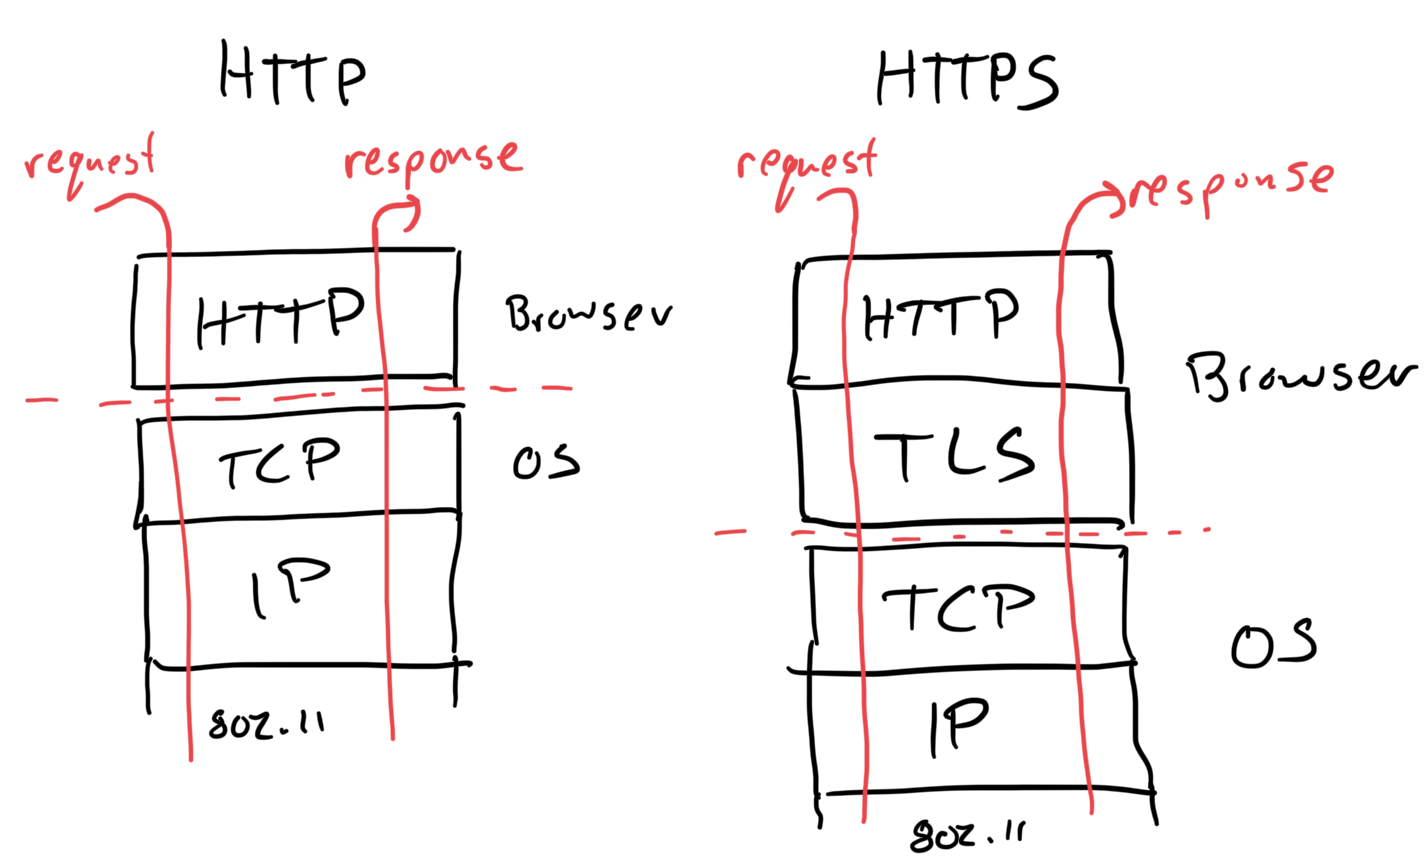
\includegraphics{im/http-tls.png}
\caption{The difference between HTTP and HTTPS is the addition of a TLS layer.}\label{fig:HttpHttps}
\end{figure}

Luckily, the Python \texttt{ssl} library implements all of these details
for us, so making an encrypted connection is almost as easy as making a
regular connection. That ease of use comes with accepting some default
settings which could be inappropriate for some situations, but for
teaching purposes they are fine.

Making an encrypted connection with \texttt{ssl} is pretty easy. Suppose
you've already created a socket, \texttt{s}, and connected it to
\texttt{example.org}. To encrypt the connection, you use
\texttt{ssl.create\_default\_context} to create a \emph{context}
\texttt{ctx} and use that context to \emph{wrap} the socket \texttt{s}:
\begin{bookblock*}{notcode}
\begin{Shaded}
\begin{Highlighting}[]
\ImportTok{import}\NormalTok{ ssl}
\NormalTok{ctx }\OperatorTok{=}\NormalTok{ ssl.create\_default\_context()}
\NormalTok{s }\OperatorTok{=}\NormalTok{ ctx.wrap\_socket(s, server\_hostname}\OperatorTok{=}\NormalTok{host)}
\end{Highlighting}
\end{Shaded}
\end{bookblock*}
\noindent Note that \texttt{wrap\_socket} returns a new socket, which I save back
into the \texttt{s} variable. That's because you don't want to send any
data over the original socket; it would be unencrypted and also
confusing. The \texttt{server\_hostname} argument is used to check that
you've connected to the right server. It should match the \texttt{Host}
header.

\begin{bookblock}{installation}
On macOS, you'll need to
\href{https://stackoverflow.com/questions/52805115/certificate-verify-failed-unable-to-get-local-issuer-certificate}{run
a program called ``Install Certificates''} before you can use Python's
\texttt{ssl} package on most websites.
\end{bookblock}

Let's try to take this code and add it to \texttt{request}. First, we
need to detect which scheme is being used:
\begin{Shaded}
\begin{Highlighting}[]
\KeywordTok{class}\NormalTok{ URL:}
    \KeywordTok{def} \FunctionTok{\_\_init\_\_}\NormalTok{(}\VariableTok{self}\NormalTok{, url):}
        \VariableTok{self}\NormalTok{.scheme, url }\OperatorTok{=}\NormalTok{ url.split(}\StringTok{"://"}\NormalTok{, }\DecValTok{1}\NormalTok{)}
        \ControlFlowTok{assert} \VariableTok{self}\NormalTok{.scheme }\KeywordTok{in}\NormalTok{ [}\StringTok{"http"}\NormalTok{, }\StringTok{"https"}\NormalTok{]}
        \CommentTok{\# ...}
\end{Highlighting}
\end{Shaded}
(Note that here you're supposed to replace the existing scheme parsing
code with this new code. It's usually clear from context and the code
itself what you need to replace.)

Encrypted HTTP connections usually use port 443 instead of port 80:
\begin{Shaded}
\begin{Highlighting}[]
\KeywordTok{class}\NormalTok{ URL:}
    \KeywordTok{def} \FunctionTok{\_\_init\_\_}\NormalTok{(}\VariableTok{self}\NormalTok{, url):}
        \CommentTok{\# ...}
        \ControlFlowTok{if} \VariableTok{self}\NormalTok{.scheme }\OperatorTok{==} \StringTok{"http"}\NormalTok{:}
            \VariableTok{self}\NormalTok{.port }\OperatorTok{=} \DecValTok{80}
        \ControlFlowTok{elif} \VariableTok{self}\NormalTok{.scheme }\OperatorTok{==} \StringTok{"https"}\NormalTok{:}
            \VariableTok{self}\NormalTok{.port }\OperatorTok{=} \DecValTok{443}
\end{Highlighting}
\end{Shaded}
We can use that port when creating the socket:
\begin{Shaded}
\begin{Highlighting}[]
\KeywordTok{class}\NormalTok{ URL:}
    \KeywordTok{def}\NormalTok{ request(}\VariableTok{self}\NormalTok{):}
        \CommentTok{\# ...}
\NormalTok{        s.}\ExtensionTok{connect}\NormalTok{((}\VariableTok{self}\NormalTok{.host, }\VariableTok{self}\NormalTok{.port))}
        \CommentTok{\# ...}
\end{Highlighting}
\end{Shaded}

Next, we'll wrap the socket with the \texttt{ssl} library:
\begin{Shaded}
\begin{Highlighting}[]
\KeywordTok{class}\NormalTok{ URL:}
    \KeywordTok{def}\NormalTok{ request(}\VariableTok{self}\NormalTok{):}
        \CommentTok{\# ...}
        \ControlFlowTok{if} \VariableTok{self}\NormalTok{.scheme }\OperatorTok{==} \StringTok{"https"}\NormalTok{:}
\NormalTok{            ctx }\OperatorTok{=}\NormalTok{ ssl.create\_default\_context()}
\NormalTok{            s }\OperatorTok{=}\NormalTok{ ctx.wrap\_socket(s, server\_hostname}\OperatorTok{=}\VariableTok{self}\NormalTok{.host)}
        \CommentTok{\# ...}
\end{Highlighting}
\end{Shaded}
Your browser should now be able to connect to HTTPS sites.

While we're at it, let's add support for custom ports, which are
specified in a URL by putting a colon after the host name, as in Figure~\ref{fig:UrlPort}.

\begin{figure}[b!]
\centering
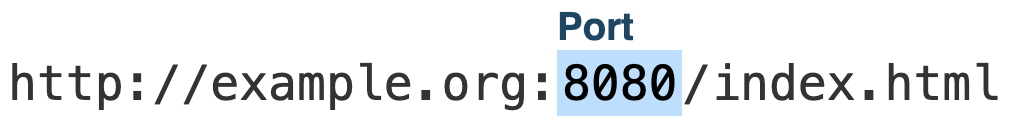
\includegraphics[width=0.7\textwidth]{im/http-ports.png}
\caption{Where the port goes in a URL.}\label{fig:UrlPort}
\end{figure}

If the URL has a port we can parse it out and use it:
\begin{Shaded}
\begin{Highlighting}[]
\KeywordTok{class}\NormalTok{ URL:}
    \KeywordTok{def} \FunctionTok{\_\_init\_\_}\NormalTok{(}\VariableTok{self}\NormalTok{, url):}
        \CommentTok{\# ...}
        \ControlFlowTok{if} \StringTok{":"} \KeywordTok{in} \VariableTok{self}\NormalTok{.host:}
            \VariableTok{self}\NormalTok{.host, port }\OperatorTok{=} \VariableTok{self}\NormalTok{.host.split(}\StringTok{":"}\NormalTok{, }\DecValTok{1}\NormalTok{)}
            \VariableTok{self}\NormalTok{.port }\OperatorTok{=} \BuiltInTok{int}\NormalTok{(port)}
\end{Highlighting}
\end{Shaded}

Custom ports are handy for debugging. Python has a built-in web server
you can use to serve files on your computer. For example, if you run
\begin{verbatim}
python3 -m http.server 8000 -d /some/directory
\end{verbatim}
then going to \texttt{http://localhost:8000/} should show you all the
files in that directory. This is a good way to test your browser.

\begin{bookblock}{further}
TLS is pretty complicated. You can read the details in
\href{https://tools.ietf.org/html/rfc8446}{RFC~8446}, but implementing
your own is not recommended. It's very difficult to write a custom TLS
implementation that is not only correct but secure.
\end{bookblock}

At this point you should be able to run your program on any web page.
Here is what it should output for
\href{https://browser.engineering/examples/example1-simple.html}{a simple example}:
\begin{bookblock*}{notcode}
\begin{Shaded}
\begin{Highlighting}[]
\NormalTok{    This is a simple}
\NormalTok{    web page with some}
\NormalTok{    text in it.}
\end{Highlighting}
\end{Shaded}
\end{bookblock*}

\hypertarget{summary}{%
\section{Summary}\label{DownloadingWebPages-summary}}

This chapter went from an empty file to a rudimentary web browser that
can:
\begin{itemize}
\tightlist
\item
  parse a URL into a scheme, host, port, and path;
\item
  connect to that host using the \texttt{sockets} and \texttt{ssl}
  libraries;
\item
  send an HTTP request to that host, including a \texttt{Host} header;
\item
  split the HTTP response into a status line, headers, and a body;
\item
  print the text (and not the tags) in the body.
\end{itemize}
Yes, this is still more of a command-line tool than a web browser, but
it already has some of the core capabilities of a browser.

\hypertarget{outline}{%
\section{Outline}\label{DownloadingWebPages-outline}}

The complete set of functions, classes, and methods in our browser
should look something like this:
\begin{Shaded}
\begin{Highlighting}[]
\KeywordTok{class}\NormalTok{ URL:}
    \KeywordTok{def} \FunctionTok{\_\_init\_\_}\NormalTok{(url)}
    \KeywordTok{def}\NormalTok{ request()}
\KeywordTok{def}\NormalTok{ show(body)}
\KeywordTok{def}\NormalTok{ load(url)}
\end{Highlighting}
\end{Shaded}

\hypertarget{exercises}{%
\section{Exercises}\label{DownloadingWebPages-exercises}}

\begin{enumerate}[label=\thechapter-\arabic*]
\item\label{ex:HTTP/1.1} \emph{HTTP/1.1.} Along with \texttt{Host}, send the \texttt{Connection}
header in the \texttt{request} function with the value \texttt{close}.
Your browser can now declare that it is using \texttt{HTTP/1.1}. Also
add a \texttt{User-Agent} header. Its value can be whatever you
want---it identifies your browser to the host. Make it easy to add
further headers in the future.

\item \emph{File URLs.} Add support for the \texttt{file} scheme, which allows
the browser to open local files. For example,
\texttt{file:///path/goes/here} should refer to the file on your
computer at location \texttt{/path/goes/here}. Also make it so that, if
your browser is started without a URL being given, some specific file on
your computer is opened. You can use that file for quick testing.

\item \emph{\texttt{data}.} Yet another scheme is \texttt{data}, which allows inlining
HTML content into the URL itself. Try navigating to
\texttt{data:text/html,Hello\ world!} in a real browser to see what
happens. Add support for this scheme to your browser. The \texttt{data}
scheme is especially convenient for making tests without having to put
them in separate files.

\item\label{ex:Entities} \emph{Entities.} Implement support for the less-than (\texttt{\&lt;})
and greater-than (\texttt{\&gt;}) entities. These should be printed as
\texttt{\textless{}} and \texttt{\textgreater{}}, respectively. For
example, if the HTML response was \texttt{\&lt;div\&gt;}, the
\texttt{show} method of your browser should print
\texttt{\textless{}div\textgreater{}}. Entities allow web pages to
include these special characters without the browser interpreting them
as tags.

\item\label{ex:view-source}\emph{\texttt{view-source}.} Add support for the \texttt{view-source} scheme;
navigating to \texttt{view-source:http://example.org/} should show the HTML
source instead of the rendered page. Add support for this scheme. Your
browser should print the entire HTML file as if it was text. You'll want
to have also implemented % the entities
Exercise~\ref{ex:Entities}.

\item \emph{Keep-alive.} Implement % the HTTP/1.1
  Exercise~\ref{ex:HTTP/1.1}; however, do not send
the \texttt{Connection:\ close} header. Instead, when reading the body
from the socket, only read as many bytes as given in the
\texttt{Content-Length} header and don't close the socket afterward.
Instead, save the socket, and if another request is made to the same
socket reuse the same socket instead of creating a new one. This will
speed up repeated requests to the same server, which is common.

\item \emph{Redirects.} Error codes in the 300 range request a redirect. When
your browser encounters one, it should make a new request to the URL
given in the \texttt{Location} header. Sometimes the \texttt{Location}
header is a full URL, but sometimes it skips the host and scheme and
just starts with a \texttt{/} (meaning the same host and scheme as the
original request). The new URL might itself be a redirect, so make sure
to handle that case. You don't, however, want to get stuck in a redirect
loop, so make sure to limit how many redirects your browser can follow in a
row. You can test this with the URL
\url{http://browser.engineering/redirect}, which redirects back to this
page, and its \href{http://browser.engineering/redirect2}{/redirect2} and
\href{http://browser.engineering/redirect3}{/redirect3} cousins which
do more complicated redirect chains.

\item \emph{Caching.} Typically, the same images, styles, and scripts are used
on multiple pages; downloading them repeatedly is a waste. It's
generally valid to cache any HTTP response, as long as it was requested
with \texttt{GET} and received a \texttt{200} response.\footnote{Some
  other status codes like \texttt{301} and \texttt{404} can also be
  cached.} Implement a cache in your browser and test it by requesting
the same file multiple times. Servers control caches using the
\texttt{Cache-Control} header. Add support for this header, specifically
for the \texttt{no-store} and \texttt{max-age} values. If the
\texttt{Cache-Control} header contains any value other than these two,
it's best not to cache the response.

\item \emph{Compression.} Add support for HTTP compression, in which the
browser
\href{https://developer.mozilla.org/en-US/docs/Web/HTTP/Content_negotiation}{informs
the server} that compressed data is acceptable. Your browser must send
the \texttt{Accept-Encoding} header with the value \texttt{gzip}. If the
server supports compression, its response will have a
\texttt{Content-Encoding} header with value \texttt{gzip}. The body is
then compressed. Add support for this case. To decompress the data, you
can use the \texttt{decompress} method in the \texttt{gzip} module. GZip
data is not \texttt{utf8}-encoded, so pass \texttt{"rb"} to
\texttt{makefile} to work with raw bytes instead. Most web servers send
compressed data in a \texttt{Transfer-Encoding} called
\href{https://developer.mozilla.org/en-US/docs/Web/HTTP/Headers/Transfer-Encoding}{\texttt{chunked}}.
You'll need to add support for that, too.\footnote{There are also a couple
  of \texttt{Transfer-Encoding}s that compress the data. They aren't
  commonly used.}
\end{enumerate}

\ifprintedoutput
\theendnotes
\setcounter{endnote}{0}
\fi

\chapter{Drawing to the Screen}\label{ch:DrawingToTheScreen}
A web browser doesn't just download a web page; it also has to show that
page to the user. In the % 21\textsuperscript{st}
twenty-first century, that means a
graphical application. So in this chapter we'll equip our browser with a
graphical user interface.\footnote{There are some obscure text-based
  browsers: I used \texttt{w3m} as my main browser for most of 2011. I
  don't anymore.}

\hypertarget{creating-windows}{%
\section{Creating Windows}\label{creating-windows}}

Desktop and laptop computers run operating systems that provide
\emph{desktop environments}: windows, buttons, and a mouse. So
responsibility ends up split: programs control their window, but the
desktop environment controls the screen. Therefore:
\begin{itemize}
%\tightlist
\item
  The program asks for a new window and the desktop environment actually
  displays it.
\item
  The program draws to its window and the desktop environment puts that
  on the screen.
\item
  The desktop environment tells the program about clicks and key
  presses, and the program responds and redraws its window.
\end{itemize}

Doing all of this by hand is a bit of a drag, so programs usually use a
\emph{graphical toolkit} to simplify these steps. Python comes with a
graphical toolkit called Tk\index{Tk} using the Python package
\texttt{tkinter}.\footnote{The library is called Tk, and it was
  originally written for a different language called Tcl. Python
  contains an interface to it, hence the name.}\index{Tkinter} Using it
is quite simple:
\begin{Shaded}
\begin{Highlighting}[]
\ImportTok{import}\NormalTok{ tkinter}
\NormalTok{window }\OperatorTok{=}\NormalTok{ tkinter.Tk()}
\NormalTok{tkinter.mainloop()}
\end{Highlighting}
\end{Shaded}
Here, \texttt{tkinter.Tk()} asks the desktop environment to create a
window and returns an object that you can use to draw to the window. The
\texttt{tkinter.mainloop()} call enters a loop that looks like
this:\footnote{This pseudocode may look like an infinite loop that locks
  up the computer, but it's not. Either the operating system will
  multitask among threads and processes, or the \texttt{pendingEvents}
  call will sleep until events are available, or both; in any case,
  other code will run and create events for the loop to respond to.}
\begin{Shaded}
\begin{Highlighting}[]
\ControlFlowTok{while} \VariableTok{True}\NormalTok{:}
    \ControlFlowTok{for}\NormalTok{ evt }\KeywordTok{in}\NormalTok{ pendingEvents():}
\NormalTok{        handleEvent(evt)}
\NormalTok{    drawScreen()}
\end{Highlighting}
\end{Shaded}

\begin{figure}[tbp]
\centering
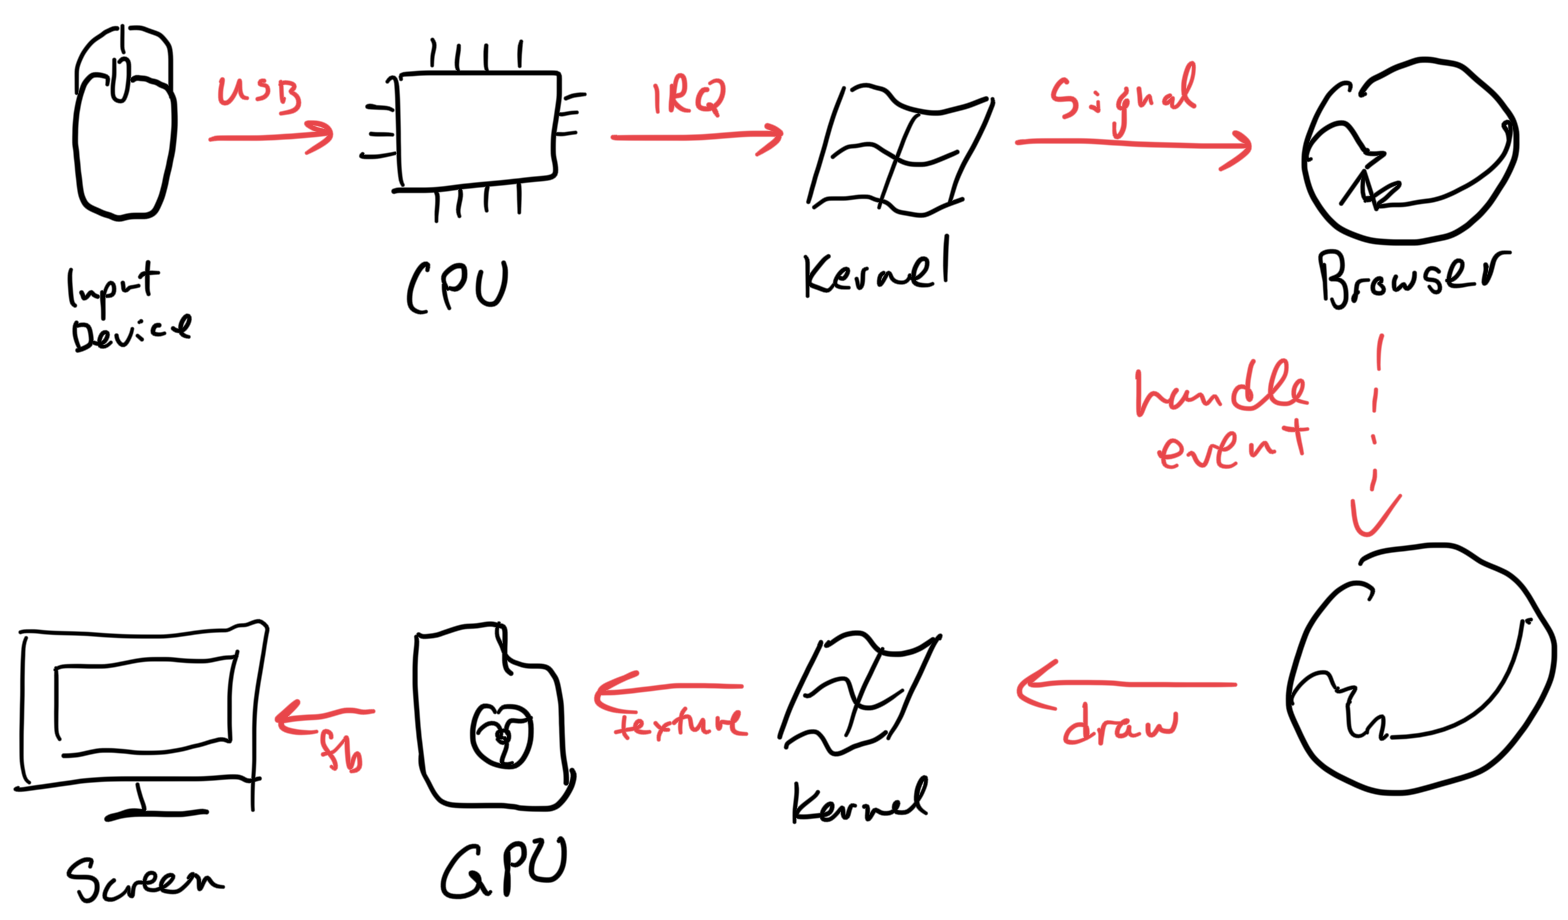
\includegraphics{im/graphics-cycle.png}
\caption{Flowchart of an event-handling cycle.}\label{fig:EventLoop}
\end{figure}

Here, \texttt{pendingEvent} first asks the desktop environment for
recent mouse clicks or key presses, then \texttt{handleEvent} calls your
application to update state, and then \texttt{drawScreen} redraws the
window. This \emph{event loop}\index{event!loop} pattern (see Figure~\ref{fig:EventLoop}) is common in
many applications, from web browsers to video games, because in complex
graphical applications it ensures that all events are eventually handled
and the screen is eventually updated.

\begin{bookblock}{further}
Although you're probably writing your browser on a desktop computer, many
people access the web through mobile devices such as phones or tablets.
On mobile devices there's still a screen, a rendering loop, and most
other things discussed in this book.\footnotemark

But there are several differences worth noting. Applications are usually
full-screen, with only one application drawing to the screen at a time.
There's no mouse and only a virtual keyboard, so the main form of
interaction is touch. There is the concept of a ``visual viewport'' that is not
present on a desktop, to accommodate ``desktop-only'' and ``mobile-ready''
sites, as well as pinch zoom.\footnotemark\ And screen pixel density is much higher,
but the total screen resolution is usually lower. Supporting all of
these differences is doable, but quite a bit of work. This book won't go
further into implementing them, except in some cases as exercises.

Also, power efficiency is much more important, because the device runs
on a battery, while at the same time the central processing unit (CPU) and memory are
significantly slower and less capable. That makes it much more important
to take advantage of any graphical processing unit (GPU)---the slow CPU makes good
performance harder to achieve. Mobile browsers are challenging!
\end{bookblock}
\footnotetext[\numexpr(\value{footnote}-1)]{
For example, most
  real browsers have both desktop and mobile editions, and the rendering
  engine code is almost exactly the same for both.
}
\footnotetext{
Look at the
  source of \href{https://browser.engineering/graphics.html}{this
  webpage}. In the \texttt{\textless{}head\textgreater{}} you'll see a
  ``viewport'' \texttt{\textless{}meta\textgreater{}} tag. This tag
  tells the browser that the page supports mobile devices; without it,
  the browser assumes that the site is ``desktop-only'' and renders it
  differently, such as allowing the user to use a pinch-zoom or
  double-tap gesture to focus in on one part of the page. Once zoomed
  in, the part of the page visible on the screen is the ``visual
  viewport'' and the whole documents' bounds are the ``layout
  viewport''. This is kind of a mix between zooming and scrolling that's
  usually absent on desktop.
}

\hypertarget{drawing-to-the-window}{%
\section{Drawing to the Window}\label{drawing-to-the-window}}

Our browser will draw the web page text to a
\emph{canvas},\index{canvas} a rectangular Tk widget that you can draw
circles, lines, and text on. For example, you can create a canvas with
Tk like this:\footnote{You may be familiar with the HTML
  \texttt{\textless{}canvas\textgreater{}} element, which is a similar
  idea: a two-dimensional (2D) rectangle in which you can draw shapes.}
\begin{bookblock*}{notcode}
\begin{Shaded}
\begin{Highlighting}[]
\NormalTok{WIDTH, HEIGHT }\OperatorTok{=} \DecValTok{800}\NormalTok{, }\DecValTok{600}
\NormalTok{window }\OperatorTok{=}\NormalTok{ tkinter.Tk()}
\NormalTok{canvas }\OperatorTok{=}\NormalTok{ tkinter.Canvas(window, width}\OperatorTok{=}\NormalTok{WIDTH, height}\OperatorTok{=}\NormalTok{HEIGHT)}
\NormalTok{canvas.pack()}
\end{Highlighting}
\end{Shaded}
\end{bookblock*}
\noindent The first line creates the window, % as above;
and the second creates the
\texttt{Canvas} inside that window. We pass the window as an argument,
so that Tk knows where to display the canvas. The other arguments define
the canvas's size; I chose $800\times600$ because that was a common old-timey
monitor size.\footnote{This size, called Super Video Graphics Array
  (SVGA), was standardized in 1987, and probably did seem super back
  then.} The third line is a Tk peculiarity, which positions the canvas
inside the window. Tk also has widgets like buttons and dialog boxes,
but our browser won't use them: we will need finer-grained control over
appearance, which a canvas provides.\footnote{This is why desktop
  applications are more uniform than web pages: desktop applications
  generally use widgets provided by a common graphical toolkit, which
  makes them look similar.}

To keep it all organized let's put this code in a class:
\begin{Shaded}
\begin{Highlighting}[]
\KeywordTok{class}\NormalTok{ Browser:}
    \KeywordTok{def} \FunctionTok{\_\_init\_\_}\NormalTok{(}\VariableTok{self}\NormalTok{):}
        \VariableTok{self}\NormalTok{.window }\OperatorTok{=}\NormalTok{ tkinter.Tk()}
        \VariableTok{self}\NormalTok{.canvas }\OperatorTok{=}\NormalTok{ tkinter.Canvas(}
            \VariableTok{self}\NormalTok{.window, }
\NormalTok{            width}\OperatorTok{=}\NormalTok{WIDTH,}
\NormalTok{            height}\OperatorTok{=}\NormalTok{HEIGHT}
\NormalTok{        )}
        \VariableTok{self}\NormalTok{.canvas.pack()}
\end{Highlighting}
\end{Shaded}

Once you've made a canvas, you can call methods that draw shapes on the
canvas. Let's do that inside \texttt{load}, which we'll move into the
new \texttt{Browser} class:
\begin{Shaded}
\begin{Highlighting}[]
\KeywordTok{class}\NormalTok{ Browser:}
    \KeywordTok{def}\NormalTok{ load(}\VariableTok{self}\NormalTok{, url):}
        \CommentTok{\# ...}
        \VariableTok{self}\NormalTok{.canvas.create\_rectangle(}\DecValTok{10}\NormalTok{, }\DecValTok{20}\NormalTok{, }\DecValTok{400}\NormalTok{, }\DecValTok{300}\NormalTok{)}
        \VariableTok{self}\NormalTok{.canvas.create\_oval(}\DecValTok{100}\NormalTok{, }\DecValTok{100}\NormalTok{, }\DecValTok{150}\NormalTok{, }\DecValTok{150}\NormalTok{)}
        \VariableTok{self}\NormalTok{.canvas.create\_text(}\DecValTok{200}\NormalTok{, }\DecValTok{150}\NormalTok{, text}\OperatorTok{=}\StringTok{"Hi!"}\NormalTok{)}
\end{Highlighting}
\end{Shaded}

To run this code, create a \texttt{Browser}, call \texttt{load}, and
then start the Tk \texttt{mainloop}:
\begin{Shaded}
\begin{Highlighting}[]
\ControlFlowTok{if} \VariableTok{\_\_name\_\_} \OperatorTok{==} \StringTok{"\_\_main\_\_"}\NormalTok{:}
    \ImportTok{import}\NormalTok{ sys}
\NormalTok{    Browser().load(URL(sys.argv[}\DecValTok{1}\NormalTok{]))}
\NormalTok{    tkinter.mainloop()}
\end{Highlighting}
\end{Shaded}
You ought to see: a rectangle, starting near the top-left corner of the
canvas and ending at its center; then a circle inside that rectangle;
and then the text ``Hi!'' next to the circle, as in Figure~\ref{fig:TkExample}.

% \begin{center}

\begin{figure}[tbp]
\centering
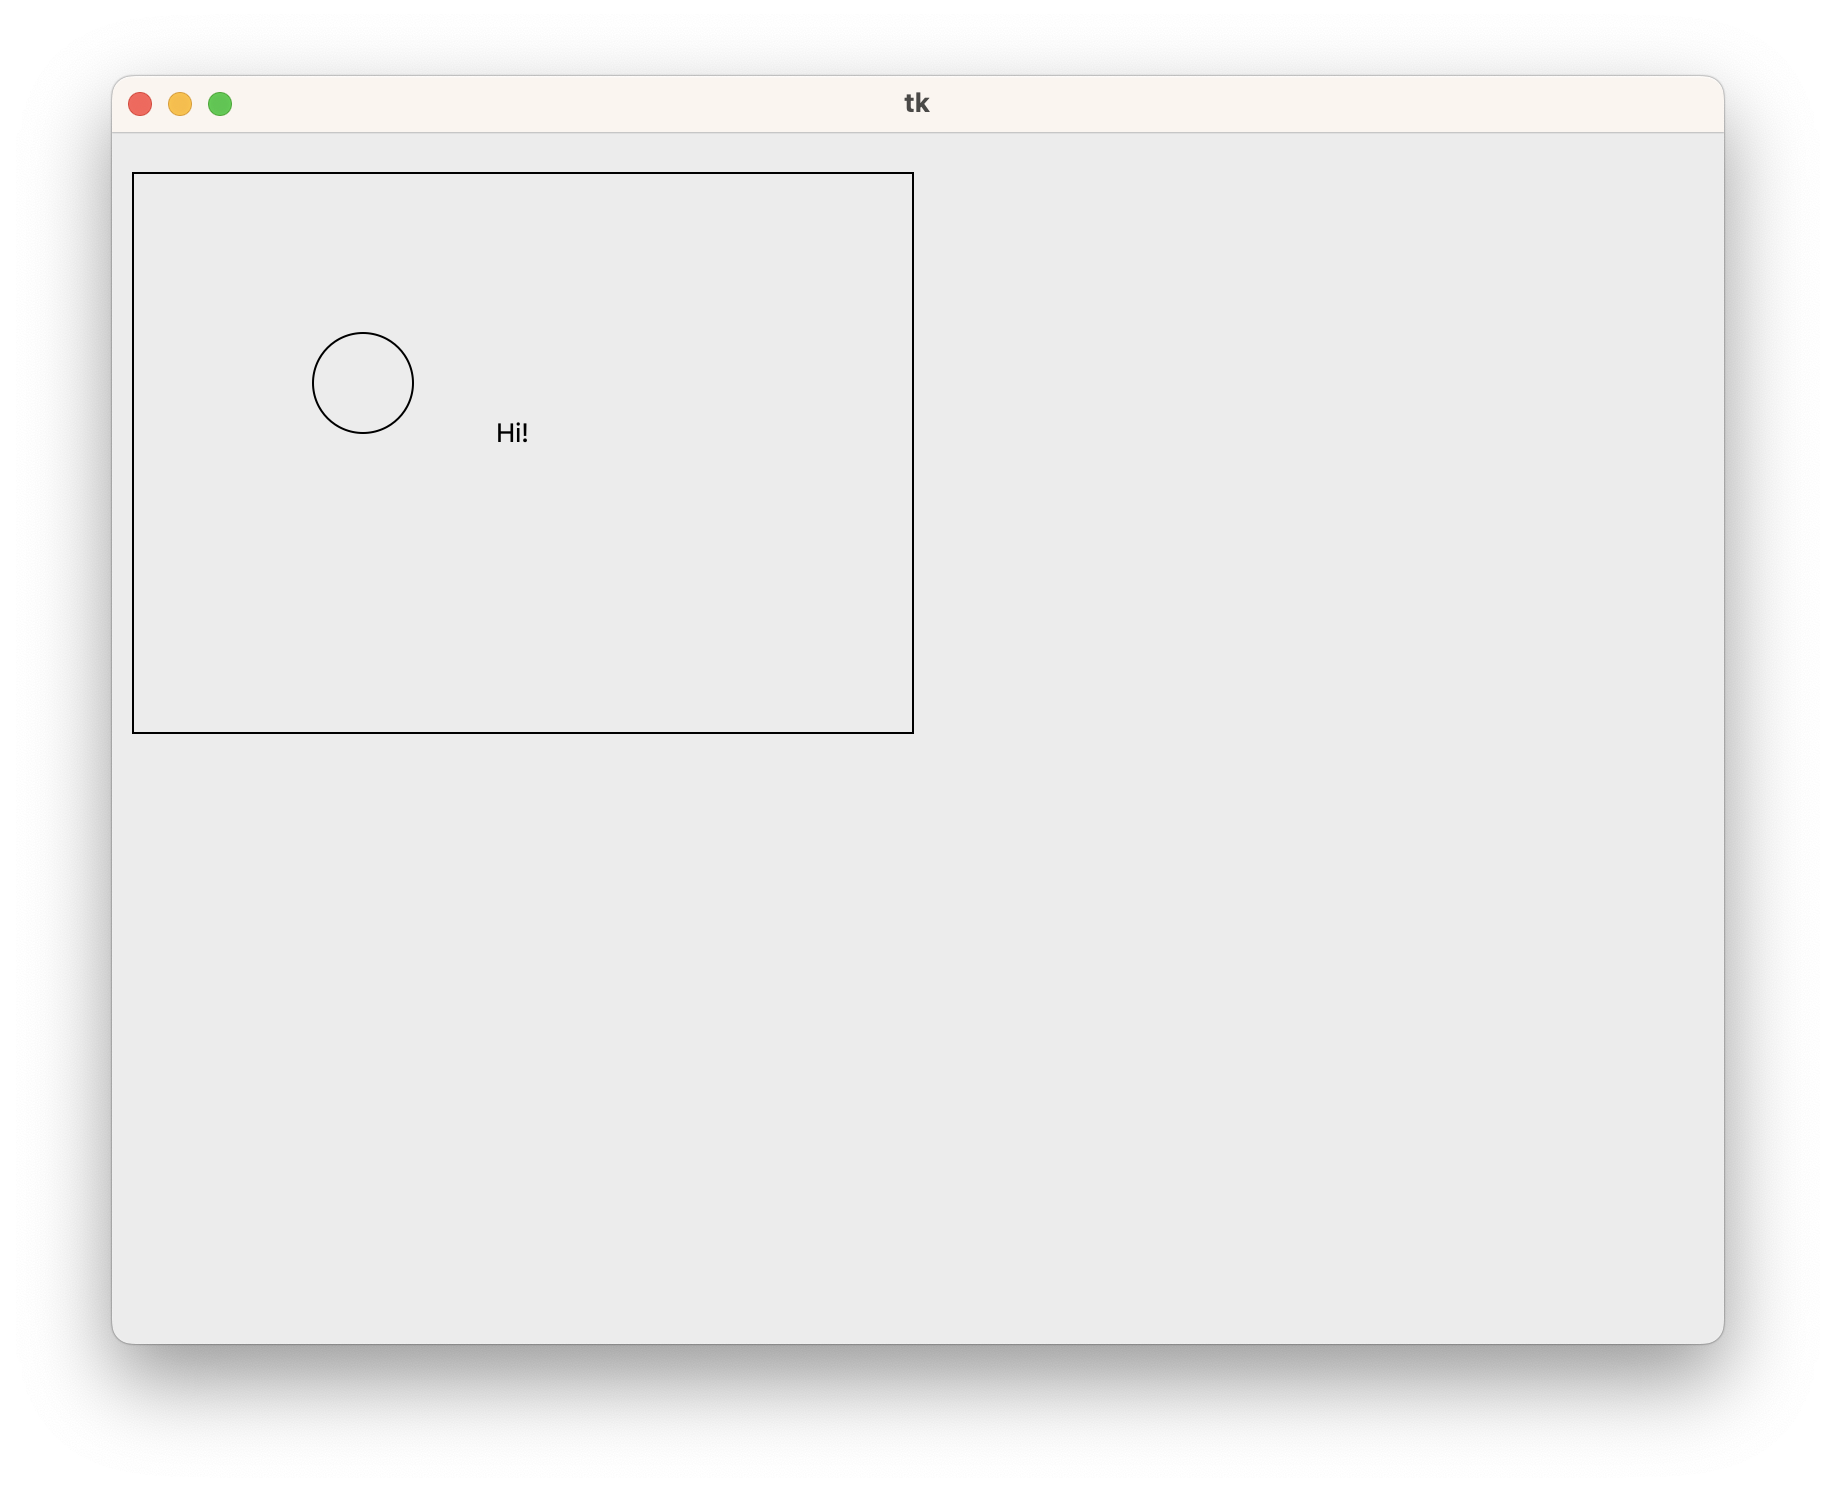
\includegraphics[width=0.895\textwidth]{im/graphics-example.png}
\caption{The expected example output with a rectangle, circle, and text.}\label{fig:TkExample}
\end{figure}

%\end{center}

Coordinates in Tk refer to $x$ positions from left to right and % to
$y$ positions from top to bottom. In other words, the bottom of the screen
has \emph{larger} $y$ values, the opposite of what you might be used to
from math. Play with the coordinates above to figure out what each
argument refers to.\footnote{The answers are in the
  \href{https://anzeljg.github.io/rin2/book2/2405/docs/tkinter/canvas.html}{online
  documentation}.}

\begin{bookblock}{further}
The Tk canvas widget is quite a bit more powerful than what we're using
it for here. As you can see from
\href{https://tkdocs.com/tutorial/canvas.html}{the tutorial}, you can
move the individual things you've drawn to the canvas, listen to click
events on each one, and so on. I'm not using those
features in this book, because I want to teach you how to implement them.
\end{bookblock}

\hypertarget{laying-out-text}{%
\section{Laying Out Text}\label{laying-out-text}}

Let's draw a simple web page on this canvas. So far, our browser steps
through the web page source code character by character and prints the
text (but not the tags) to the console window. Now we want to draw the
characters on the canvas instead.

To start, let's change the \texttt{show} function from the previous
chapter into a function that I'll call \texttt{lex}\footnote{Foreshadowing
  future developments\ldots{}} which just \emph{returns} the textual
content of an HTML document without printing it:
\begin{Shaded}
\begin{Highlighting}[]
\KeywordTok{def}\NormalTok{ lex(body):}
\NormalTok{  text }\OperatorTok{=} \StringTok{""}
  \CommentTok{\# ...}
  \ControlFlowTok{for}\NormalTok{ c }\KeywordTok{in}\NormalTok{ body:}
      \CommentTok{\# ...}
      \ControlFlowTok{elif} \KeywordTok{not}\NormalTok{ in\_tag:}
\NormalTok{          text }\OperatorTok{+=}\NormalTok{ c}
    \ControlFlowTok{return}\NormalTok{ text}
\end{Highlighting}
\end{Shaded}
Then, \texttt{load} will draw that text, character by character:
\begin{Shaded}
\begin{Highlighting}[]
\KeywordTok{def}\NormalTok{ load(}\VariableTok{self}\NormalTok{, url):}
    \CommentTok{\# ...}
    \ControlFlowTok{for}\NormalTok{ c }\KeywordTok{in}\NormalTok{ text:}
        \VariableTok{self}\NormalTok{.canvas.create\_text(}\DecValTok{100}\NormalTok{, }\DecValTok{100}\NormalTok{, text}\OperatorTok{=}\NormalTok{c)}
\end{Highlighting}
\end{Shaded}

Let's test this code on a real web page. For reasons that might seem
inscrutable\footnote{It's to delay a discussion of basic typography to
  the next chapter.}, let's test it on the
\href{https://browser.engineering/examples/xiyouji.html}{first chapter of
\foreignlanguage{chinese}{西游记} or \textit{Journey to the West}}, a classic
Chinese novel about a monkey. Run this URL\footnote{
  The URLs for numbered references can be found in the ``Links'' section at the end of each chapter.}
 through \texttt{request}, \texttt{lex}, and
\texttt{load}. You should see a window with a big blob of black pixels
inset a little from the top left corner of the window.

Why a blob instead of letters? Well, of course, because we are drawing
every letter in the same place, so they all overlap! Let's fix that:
\begin{Shaded}
\begin{Highlighting}[]
\NormalTok{HSTEP, VSTEP }\OperatorTok{=} \DecValTok{13}\NormalTok{, }\DecValTok{18}
\NormalTok{cursor\_x, cursor\_y }\OperatorTok{=}\NormalTok{ HSTEP, VSTEP}
\ControlFlowTok{for}\NormalTok{ c }\KeywordTok{in}\NormalTok{ text:}
    \VariableTok{self}\NormalTok{.canvas.create\_text(cursor\_x, cursor\_y, text}\OperatorTok{=}\NormalTok{c)}
\NormalTok{    cursor\_x }\OperatorTok{+=}\NormalTok{ HSTEP}
\end{Highlighting}
\end{Shaded}
The variables \texttt{cursor\_x} and \texttt{cursor\_y} point to where
the next character will go, as if you were typing the text % with
into a
word processor. I picked the magic numbers---13 and 18---by trying a few
different values and picking one that looked most readable.\footnote{In
  the % \href{text.md}
  Chapter 3, we'll replace the magic numbers with
  font metrics.}

The text now forms a line from left to right. But with an 800-pixel-wide
canvas and 13 pixels per character, one line only fits about 60
characters. You need more than that to read a novel, so we also need to
\emph{wrap} the text once we reach the edge of the screen:
\begin{Shaded}
\begin{Highlighting}[]
\ControlFlowTok{for}\NormalTok{ c }\KeywordTok{in}\NormalTok{ text:}
    \CommentTok{\# ...}
    \ControlFlowTok{if}\NormalTok{ cursor\_x }\OperatorTok{\textgreater{}=}\NormalTok{ WIDTH }\OperatorTok{{-}}\NormalTok{ HSTEP:}
\NormalTok{        cursor\_y }\OperatorTok{+=}\NormalTok{ VSTEP}
\NormalTok{        cursor\_x }\OperatorTok{=}\NormalTok{ HSTEP}
\end{Highlighting}
\end{Shaded}
The code increases \texttt{cursor\_y} and resets
\texttt{cursor\_x}\footnote{In the olden days of typewriters, increasing
  \emph{y} meant \emph{feed}ing in a new \emph{line}, and resetting
  \emph{x} meant \emph{return}ing the \emph{carriage} that printed
  letters to the left edge of the page. So the American Standard Code for Information Interchange
  (\href{https://en.wikipedia.org/wiki/ASCII}{ASCII})
  standardized two
  separate characters---``carriage return'' and ``line feed''---for
  these operations, so that ASCII could be directly executed by
  teletypewriters. That's why headers in HTTP are separated by
  \texttt{\textbackslash{}r\textbackslash{}n}, even though modern
  computers have no mechanical carriage.} once \texttt{cursor\_x} goes
past 787 pixels.\footnote{Not 800, because we started at pixel 13 and I
  want to leave an even gap on both sides.} The sequence is shown in 
Figure~\ref{fig:CharacterDrawing}.
Wrapping the text this way
makes it possible to read more than a single line.

\begin{figure}[b!]
\centering
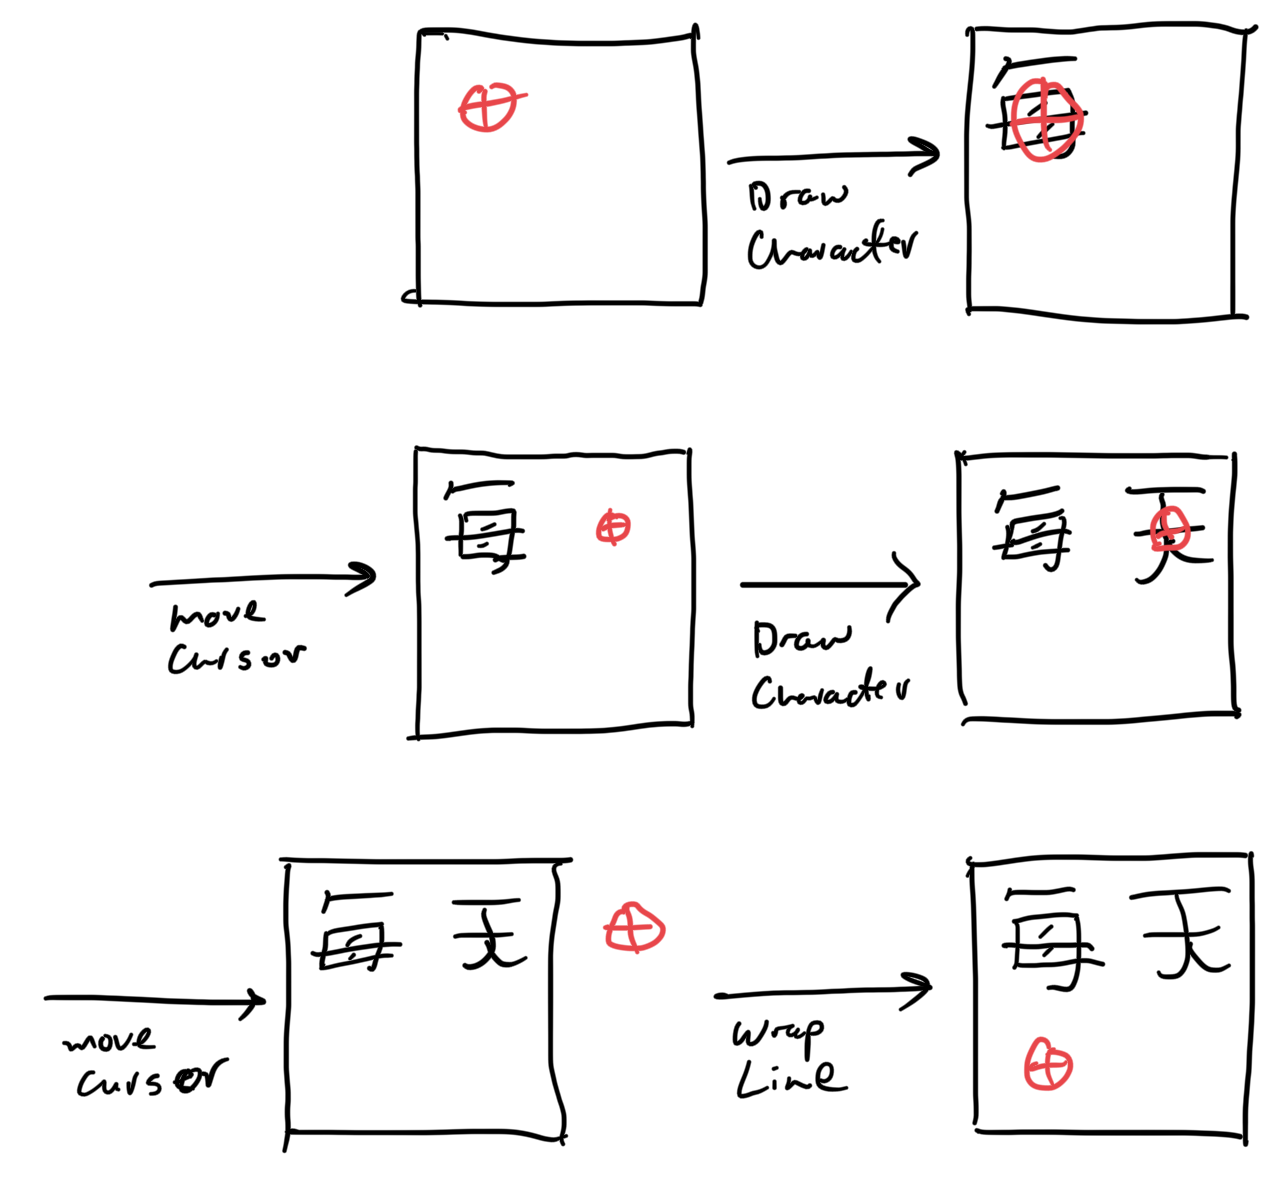
\includegraphics{im/graphics-cursor.png}
\caption{A flow-chart of how % characters
 the cursor moves as each character is drawn.}\label{fig:CharacterDrawing}
\end{figure}

At this point you should be able to load up
\href{https://browser.engineering/examples/xiyouji.html}{our example page}
in your browser and have it look
% about
something like % this:
Figure~\ref{fig:ExampleText}.

% \begin{center}
\begin{figure}
\centering
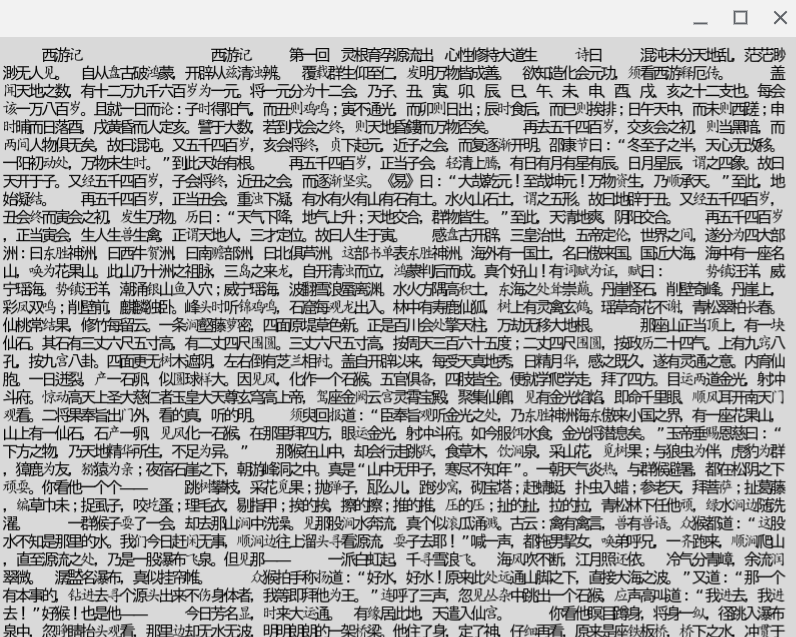
\includegraphics[width=0.9\textwidth]{examples/example2-text-screenshot.png}
\caption{The first chapter of \textit{Journey to the West} rendered in our browser.}\label{fig:ExampleText}
\end{figure}
%\end{center}

Now we can read a lot of text, but still not all of it: if there's
enough text, not all of the lines % of text don't
will  fit on the screen. We want
users to \emph{scroll}\index{scroll} the page to look at different parts
of it.

\begin{bookblock}{further}
In English text, you can't wrap to the next line in the middle of a word
(without hyphenation at least), but in Chinese that's mostly not a
problem. Mostly, but not always! \foreignlanguage{chinese}{开关} means
``button'' but is composed of \foreignlanguage{chinese}{开} ``on'' and
\foreignlanguage{chinese}{关} ``off''. A line break between them would
be confusing, because you'd read ``on off'' instead of ``button''. The
\href{http://site.icu-project.org}{ICU library}, used by both Firefox
and Chrome,
\href{https://unicode-org.github.io/icu/userguide/boundaryanalysis/break-rules.html\#details-about-dictionary-based-break-iteration}{uses
dynamic programming} to guess phrase boundaries based on a
\href{https://github.com/unicode-org/icu/blob/master/icu4c/source/data/brkitr/dictionaries/cjdict.txt}{word
frequency table}.
\end{bookblock}

\hypertarget{scrolling-text}{%
\section{Scrolling Text}\label{scrolling-text}}

Scrolling introduces a layer of indirection between page coordinates
(this text is 132 pixels from the top of the \emph{page}) and screen
coordinates (since you've scrolled 60 pixels down, this text is 72
pixels from the top of the \emph{screen})---see Figure~\ref{fig:ScreenPage}.
Generally speaking, a browser
\emph{lays out} the page---determines where everything on the page
goes---in terms of page coordinates and then \emph{renders} the
page---draws everything---in terms of screen coordinates.\footnote{Sort
  of. What actually happens is that the page is first drawn into a
  bitmap or GPU texture, then that bitmap/texture is shifted according
  to the scroll, and the result is rendered to the screen.
%  \href{visual-effects.md}
  Chapter~\ref{ch:AddingVisualEffects} will have more on this topic.}

\begin{figure}[tbp]
\centering
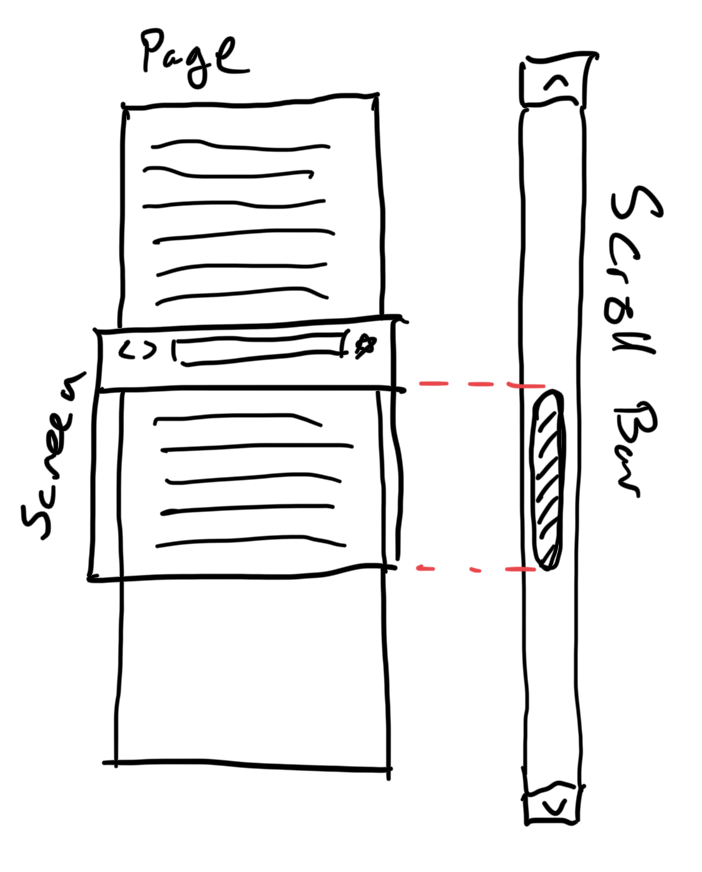
\includegraphics[width=0.5\textwidth]{im/graphics-coords.png}
\caption{The difference between page and screen coordinates.}\label{fig:ScreenPage}
\end{figure}

Our browser will have the same split. Right now \texttt{load} computes
both the position of each character and draws it: layout\index{layout}
and rendering.\index{rendering} Let's instead have a \texttt{layout}
function to compute and store the position of each character, and a
separate \texttt{draw} function to then draw each character based on the
stored position. This way, \texttt{layout} can operate with page
coordinates and only \texttt{draw} needs to think about screen
coordinates.

Let's start with \texttt{layout}. Instead of calling
\texttt{canvas.create\_text} on each character let's add it to a list,
together with its position. Since \texttt{layout} doesn't need to access
anything in \texttt{Browser}, it can be a standalone function:
\begin{Shaded}
\begin{Highlighting}[]
\KeywordTok{def}\NormalTok{ layout(text):}
\NormalTok{    display\_list }\OperatorTok{=}\NormalTok{ []}
\NormalTok{    cursor\_x, cursor\_y }\OperatorTok{=}\NormalTok{ HSTEP, VSTEP}
    \ControlFlowTok{for}\NormalTok{ c }\KeywordTok{in}\NormalTok{ text:}
\NormalTok{        display\_list.append((cursor\_x, cursor\_y, c))}
        \CommentTok{\# ...}
    \ControlFlowTok{return}\NormalTok{ display\_list}
\end{Highlighting}
\end{Shaded}
The resulting list of things to display is called a \emph{display
list}.\footnote{The term ``display list'' is standard.} Since \texttt{layout} is all about
page coordinates, we don't need to change anything else about it to
support scrolling.

Once the display list is computed, \texttt{draw} needs to loop through
it and draw each character. Since \texttt{draw} does need
access to the canvas, we make it a method on \texttt{Browser}:
\begin{Shaded}
\begin{Highlighting}[]
\KeywordTok{class}\NormalTok{ Browser:}
    \KeywordTok{def}\NormalTok{ draw(}\VariableTok{self}\NormalTok{):}
        \ControlFlowTok{for}\NormalTok{ x, y, c }\KeywordTok{in} \VariableTok{self}\NormalTok{.display\_list:}
            \VariableTok{self}\NormalTok{.canvas.create\_text(x, y, text}\OperatorTok{=}\NormalTok{c)}
\end{Highlighting}
\end{Shaded}
Now \texttt{load} just needs to call \texttt{layout} followed by
\texttt{draw}:
\begin{Shaded}
\begin{Highlighting}[]
\KeywordTok{class}\NormalTok{ Browser:}
    \KeywordTok{def}\NormalTok{ load(}\VariableTok{self}\NormalTok{, url):}
\NormalTok{        body }\OperatorTok{=}\NormalTok{ url.request()}
\NormalTok{        text }\OperatorTok{=}\NormalTok{ lex(body)}
        \VariableTok{self}\NormalTok{.display\_list }\OperatorTok{=}\NormalTok{ layout(text)}
        \VariableTok{self}\NormalTok{.draw()}
\end{Highlighting}
\end{Shaded}

Now we can add scrolling. Let's add a field for how far you've
scrolled:
\begin{Shaded}
\begin{Highlighting}[]
\KeywordTok{class}\NormalTok{ Browser:}
    \KeywordTok{def} \FunctionTok{\_\_init\_\_}\NormalTok{(}\VariableTok{self}\NormalTok{):}
        \CommentTok{\# ...}
        \VariableTok{self}\NormalTok{.scroll }\OperatorTok{=} \DecValTok{0}
\end{Highlighting}
\end{Shaded}
The page coordinate \texttt{y} then has screen coordinate
\texttt{y\ -\ self.scroll}:
\begin{Shaded}
\begin{Highlighting}[]
\KeywordTok{def}\NormalTok{ draw(}\VariableTok{self}\NormalTok{):}
    \ControlFlowTok{for}\NormalTok{ x, y, c }\KeywordTok{in} \VariableTok{self}\NormalTok{.display\_list:}
        \VariableTok{self}\NormalTok{.canvas.create\_text(x, y }\OperatorTok{{-}} \VariableTok{self}\NormalTok{.scroll, text}\OperatorTok{=}\NormalTok{c)}
\end{Highlighting}
\end{Shaded}
If you change the value of \texttt{scroll} the page will now scroll up
and down. But how does the \emph{user} change \texttt{scroll}?

Most browsers scroll the page when you press the up and down keys,
rotate the scroll wheel, drag the scroll bar, or apply a touch gesture
to the screen. To keep things simple, let's just implement the down key.

Tk allows you to \emph{bind} a function to a key, which instructs Tk to
call that function when the key is pressed. For example, to bind to the
down arrow key, write:
\begin{Shaded}
\begin{Highlighting}[]
\KeywordTok{def} \FunctionTok{\_\_init\_\_}\NormalTok{(}\VariableTok{self}\NormalTok{):}
    \CommentTok{\# ...}
    \VariableTok{self}\NormalTok{.window.bind(}\StringTok{"\textless{}Down\textgreater{}"}\NormalTok{, }\VariableTok{self}\NormalTok{.scrolldown)}
\end{Highlighting}
\end{Shaded}
Here, \texttt{self.scrolldown} is an \emph{event handler}, a function
that Tk will call whenever the down arrow key is pressed.\footnote{\texttt{scrolldown}
  is passed an \emph{event object} as an argument by Tk, but since
  scrolling down doesn't require any information about the key press
  besides the fact that it happened, \texttt{scrolldown} ignores that
  event object.} All it needs to do is increment \texttt{y} and redraw
the canvas:
\begin{Shaded}
\begin{Highlighting}[]
\NormalTok{SCROLL\_STEP }\OperatorTok{=} \DecValTok{100}

\KeywordTok{def}\NormalTok{ scrolldown(}\VariableTok{self}\NormalTok{, e):}
    \VariableTok{self}\NormalTok{.scroll }\OperatorTok{+=}\NormalTok{ SCROLL\_STEP}
    \VariableTok{self}\NormalTok{.draw()}
\end{Highlighting}
\end{Shaded}

If you try this out, you'll find that scrolling draws all the text a
second time. That's because we didn't erase the old text before drawing
the new text. Call \texttt{canvas.delete} to clear the old text:
\begin{Shaded}
\begin{Highlighting}[]
\KeywordTok{def}\NormalTok{ draw(}\VariableTok{self}\NormalTok{):}
    \VariableTok{self}\NormalTok{.canvas.delete(}\StringTok{"all"}\NormalTok{)}
    \CommentTok{\# ...}
\end{Highlighting}
\end{Shaded}
Scrolling should now work!

\begin{bookblock}{further}
Storing the display list makes scrolling faster: the browser isn't doing
\texttt{layout} every time you scroll. Modern browsers
\href{https://hacks.mozilla.org/2017/10/the-whole-web-at-maximum-fps-how-webrender-gets-rid-of-jank/}{take
this further}, retaining much of the display list even when the web page
changes due to JavaScript or user interaction.

In general, scrolling is the most common user interaction with web
pages. Real browsers have accordingly invested a \emph{tremendous}
amount of time making it fast; we'll get to some more of the ways later
in the book.
\end{bookblock}

\hypertarget{faster-rendering}{%
\section{Faster Rendering}\label{faster-rendering}}

Applications have to redraw these contents quickly for interactions to
feel fluid,\footnote{On older systems, applications drew directly to the
  screen, and if they didn't update, whatever was there last would stay
  in place, which is why in error conditions you'd often have one window
  leave ``trails'' on another. Modern systems use
  \href{https://en.wikipedia.org/wiki/Compositing_window_manager}{compositing},
  which avoids trails and also improves performance and isolation.
  Applications still redraw their window contents, though, to change
  what is displayed. % \href{animations.md}
  Chapter~\ref{ch:AnimatingAndCompositing} discusses
  compositing in more detail.} and must respond quickly to clicks and
key presses so the user doesn't get frustrated. ``Feel fluid'' can be
made more precise. Graphical applications such as browsers typically aim
to redraw at a speed equal to the refresh rate, or \emph{frame rate}, of
the screen, and/or a fixed 60\,Hz.\footnote{Most screens today have a
  refresh rate of 60\,Hz, and that is generally considered fast enough to
  look smooth. However, new hardware is increasingly appearing with
  higher refresh rates, such as 120\,Hz. It's not yet clear if browsers
  can be made that fast. Some rendering engines, games in particular,
  refresh at lower rates on purpose if they know the rendering speed
  can't keep up.} This means that the browser has to finish all its
work in less than 1/60th of a second, or 16\,ms, in order to keep up. For
this reason, 16\,ms is called the \emph{animation frame budget} of the
application.

But this scrolling is pretty slow.\footnote{How fast exactly seems to
  depend a lot on your operating system and default font.} Why? It turns
out that loading information about the shape of a character, inside
\texttt{create\_text}, takes a while. To speed up scrolling we need to
make sure to do it only when necessary (while at the same time ensuring
the pixels on the screen are always correct).

Real browsers have a lot of quite tricky optimizations for this, but for
our browser let's limit ourselves to a simple improvement: skip drawing
characters that are offscreen:
\begin{Shaded}
\begin{Highlighting}[]
\ControlFlowTok{for}\NormalTok{ x, y, c }\KeywordTok{in} \VariableTok{self}\NormalTok{.display\_list:}
    \ControlFlowTok{if}\NormalTok{ y }\OperatorTok{\textgreater{}} \VariableTok{self}\NormalTok{.scroll }\OperatorTok{+}\NormalTok{ HEIGHT: }\ControlFlowTok{continue}
    \ControlFlowTok{if}\NormalTok{ y }\OperatorTok{+}\NormalTok{ VSTEP }\OperatorTok{\textless{}} \VariableTok{self}\NormalTok{.scroll: }\ControlFlowTok{continue}
    \CommentTok{\# ...}
\end{Highlighting}
\end{Shaded}
The first \texttt{if} statement skips characters below the viewing
window; the second skips characters above it. In that second \texttt{if}
statement, \texttt{y\ +\ VSTEP} is the bottom edge of the character,
because characters that are halfway inside the viewing window still have
to be drawn.

Scrolling should now be pleasantly fast, and hopefully close to the 16\,ms
animation frame budget.\footnote{On my computer, it was still about
  double that budget, so there is work to do---we'll get to that in
  future chapters.} And because we split \texttt{layout} and
\texttt{draw}, we don't need to change \texttt{layout} at all to
implement this optimization.

\begin{bookblock}{further}
You should also keep in mind that not all web page interactions are
animations---there are also discrete actions such as mouse clicks.
Research has shown that it usually suffices to respond to a discrete
action in
\href{https://www.nngroup.com/articles/response-times-3-important-limits/}{100\,ms}---below
that threshold, most humans are not sensitive to discrete action speed.
This is very different from interactions such as scroll, where a speed of
less than 60\,Hz or so is quite noticeable. The difference between the two
has to do with the way the human mind processes movement (animation)
versus discrete action, and the time it takes for the brain to decide
upon such an action, execute it, and understand its result.
\end{bookblock}

\hypertarget{summary}{%
\section{Summary}\label{DrawingToTheScreen-summary}}

This chapter went from a rudimentary command-line browser to a graphical
user interface with text that can be scrolled. The browser now:
\begin{itemize}
\tightlist
\item
  talks to your operating system to create a window;
\item
  lays out the text and draws it to that window;
\item
  listens for keyboard commands;
\item
  scrolls the window in response.
\end{itemize}
Next, we'll make this browser work on English text, with all its
complexities of variable-width characters, line layout, and formatting.

\hypertarget{outline}{%
\section{Outline}\label{DrawingToTheScreen-outline}}

The complete set of functions, classes, and methods in our browser
should look something like this:
\begin{Shaded}
\begin{Highlighting}[]
\KeywordTok{class}\NormalTok{ URL:}
    \KeywordTok{def} \FunctionTok{\_\_init\_\_}\NormalTok{(url)}
    \KeywordTok{def}\NormalTok{ request()}
\KeywordTok{def}\NormalTok{ lex(body)}
\NormalTok{WIDTH}
\NormalTok{HEIGHT}
\NormalTok{HSTEP}
\NormalTok{VSTEP}
\NormalTok{SCROLL\_STEP}
\KeywordTok{def}\NormalTok{ layout(text)}
\KeywordTok{class}\NormalTok{ Browser:}
    \KeywordTok{def} \FunctionTok{\_\_init\_\_}\NormalTok{()}
    \KeywordTok{def}\NormalTok{ load(url)}
    \KeywordTok{def}\NormalTok{ draw()}
    \KeywordTok{def}\NormalTok{ scrolldown(e)}
\end{Highlighting}
\end{Shaded}

\hypertarget{exercises}{%
\section{Exercises}\label{DrawingToTheScreen-exercises}}
\begin{enumerate}[label=\thechapter-\arabic*]
\item \emph{Line breaks.} Change \texttt{layout} to end the current line and
start a new one when it sees a newline character. Increment \emph{y} by
more than \texttt{VSTEP} to give the illusion of paragraph breaks. There
are poems embedded in \textit{Journey to the West}; now you'll be able to
make them out.

\item \emph{Mouse wheel.} Add support for scrolling up when you hit the up
arrow. Make sure you can't scroll past the top of the page. Then bind
the \texttt{\textless{}MouseWheel\textgreater{}} event, which triggers
when you scroll with the mouse wheel.\footnote{It will also trigger with
  touchpad gestures, if you don't have a mouse.} The associated event
object has an \texttt{event.delta} value which tells you how far and in
what direction to scroll. Unfortunately, Mac and Windows give the
\texttt{event.delta} objects opposite sign and different scales, and on
Linux, scrolling instead uses the
\texttt{\textless{}Button-4\textgreater{}} and
\texttt{\textless{}Button-5\textgreater{}} events.\footnote{The
  \href{https://wiki.tcl-lang.org/page/mousewheel}{Tk manual} has more
  information about this. Cross-platform applications are much harder to
  write than cross-browser ones!}

\item\label{ex:Resizing} \emph{Resizing.} Make the browser resizable. To do so,
\href{https://web.archive.org/web/20201111222645id_/http://effbot.org/tkinterbook/pack.htm}{pass
the \texttt{fill} and \texttt{expand} arguments} to
\texttt{canvas.pack}, and call and bind to the
\texttt{\textless{}Configure\textgreater{}} event, which happens when
the window is resized. The window's new width and height can be found in
the \texttt{width} and \texttt{height} fields on the event object.
Remember that when the window is resized, the line breaks must change,
so you will need to call \texttt{layout} again.

\item \emph{Scrollbar.} Stop your browser from scrolling down past the last
display list entry.\footnote{This is not quite right in a real browser;
  the browser needs to account for extra whitespace at the bottom of the
  screen or the possibility of objects purposefully drawn offscreen. In
%  \href{layout.md}
  Chapter~\ref{ch:LayingOutPages} we'll implement this correctly.} At the
right edge of the screen, draw a blue, rectangular scrollbar. Make sure
the size and position of the scrollbar reflects what part of the full
document the browser can see, as in % the
Figure~\ref{fig:ScreenPage}. % showing page and screen coordinates.
 Hide the scrollbar if the whole document fits onscreen.

\item \emph{Emoji.} Add support for emoji to your browser \smiley. Emoji are
characters, and you can call \texttt{create\_text} to draw them, but the
results aren't very good. Instead, head to
\href{https://openmoji.org}{the OpenMoji project}, download the emoji
for \href{https://openmoji.org/library/\#emoji=1F600}{``grinning face''}
as a PNG file, resize it to $16\times16$ pixels, and save it to
the same folder as the browser. Use Tk's \texttt{PhotoImage} class to
load the image and then the \texttt{create\_image} method to draw it to
the canvas. In fact, download the whole OpenMoji library (look for the
``Get OpenMojis'' button at the top right)---then your browser can look
up whatever emoji is used in the page.

\item \emph{\texttt{about:blank}.} Currently, a malformed URL causes the browser to
crash. It would be much better to have error recovery for that, and
instead show a blank page, so that the user can fix the error. To do
this, add support for the special \texttt{about:blank} URL, which should
just render a blank page, and cause malformed URLs to automatically
render as if they were \texttt{about:blank}.

\item \emph{Alternate text direction.} Not all languages read and lay out from
left to right. Arabic, Persian, and Hebrew are good examples of
right-to-left languages. Implement basic support for this with a
command-line flag to your browser.\footnote{Once we get to
%  \href{html.md}
  Chapter~\ref{ch:DocumentTree} you could write it in terms of the
  \href{https://developer.mozilla.org/en-US/docs/Web/HTML/Global_attributes/dir}{\texttt{dir}}
  attribute on the \texttt{\textless{}body\textgreater{}} element.}
English sentences should still lay out left-to-right, but they should
grow from the right side of the screen (load
\href{https://browser.engineering/examples/example2-rtl.html}{this example} in your favorite browser
to see what I mean).\footnote{Sentences in an actual % RTL
right-to-left language should
  do the opposite. And then there is vertical writing mode for some East
  Asian languages like Chinese and Japanese.}
\end{enumerate}

\ifprintedoutput
\theendnotes
\setcounter{endnote}{0}
\fi

\chapter{Formatting Text}\label{ch:FormattingText}
In the last chapter, our browser created a graphical window and drew a
grid of characters to it. That's OK for Chinese, but English text
features characters of different widths grouped into words that you
can't break across lines.\footnote{There are lots of languages in the
  world, and lots of typographic conventions. A real web browser
  supports every language from Arabic to Zulu, but this book focuses on
  English. Text is near-infinitely complex, but this book cannot be
  infinitely long!} In this chapter, we'll add those capabilities.
You'll even be able to read \href{https://browser.engineering/text.html}{this page}!

\hypertarget{what-is-a-font}{%
\section{What Is a Font?}\label{what-is-a-font}}

So far, we've called \texttt{create\_text} with a character and two
coordinates to write text to the screen. But we never specified the
font\index{font}, the size, or the color. To talk about those things, we
need to create and use font objects.

What is a \emph{font}, exactly? Well, in the olden days, printers
arranged little metal slugs on rails, covered them with ink, and pressed
them to a sheet of paper, creating a printed page (see Figure~\ref{fig:Printers}). The metal shapes came
in boxes, one per letter, so you'd have a (large) box of e's, a (small)
box of x's, and so on. The boxes came in cases (see Figure~\ref{fig:TypeCases}), one for upper-\emph{case}
and one for lower-\emph{case} letters. The set of cases was called a
font.\footnote{The word is related to \emph{foundry}, which would create
  the little metal shapes.} Naturally, if you wanted to print larger
text, you needed different (bigger) shapes, so those were a different
font; a collection of fonts was called a \emph{type}, which is why we
call it typing. Variations---like bold or italic letters---were called
that type's ``faces''.

% \begin{center}

\begin{figure}
\centering
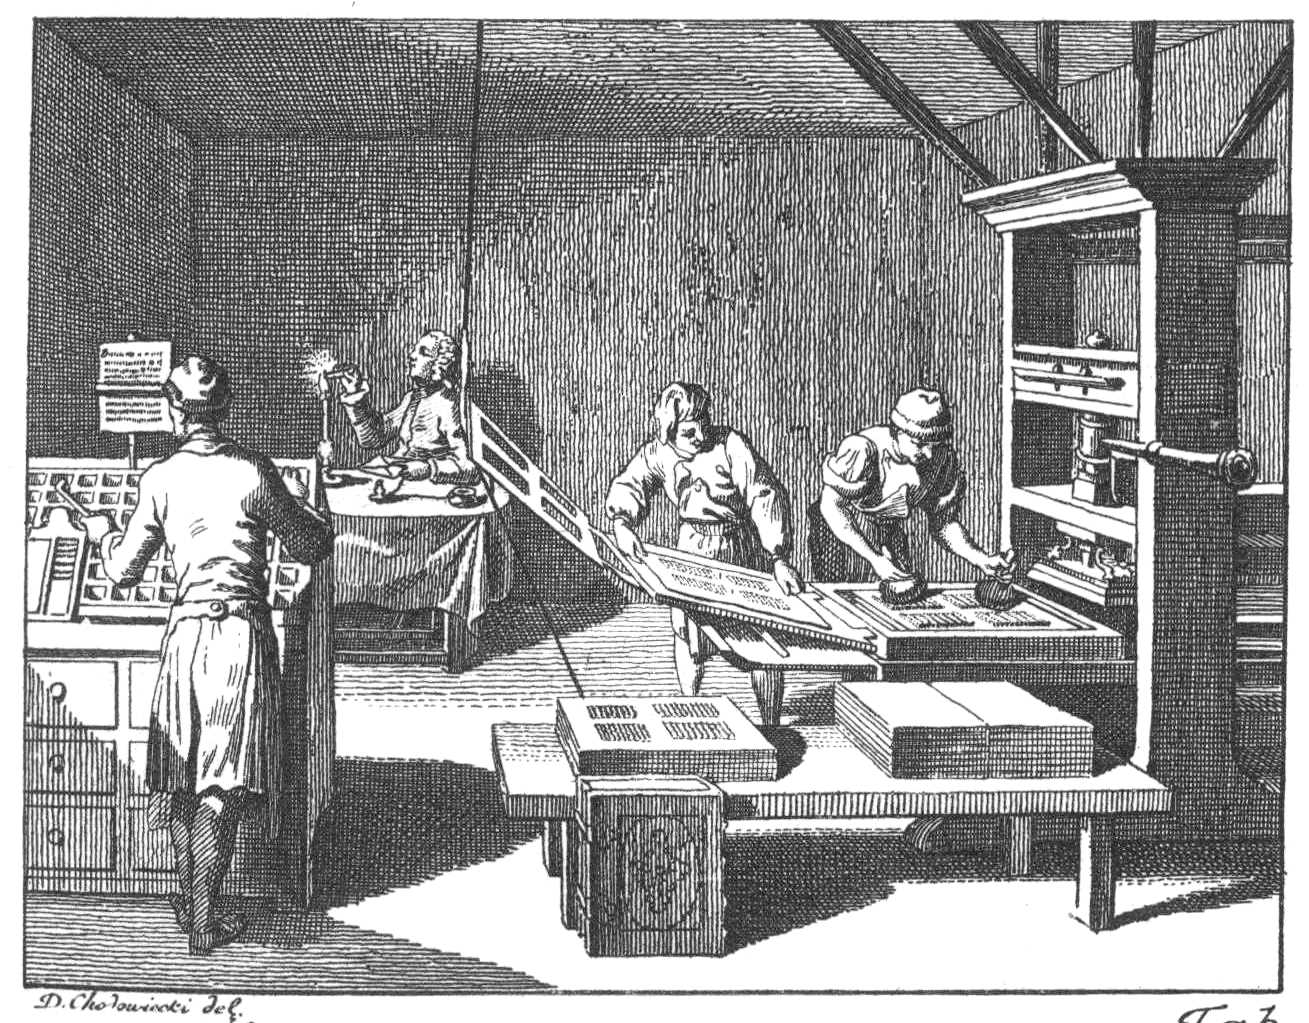
\includegraphics[width=0.8\textwidth]{im/text-old.jpeg}
\caption{A drawing of printing press workers. (By
\href{https://en.wikipedia.org/wiki/Daniel_Chodowiecki}{Daniel Nikolaus
Chodowiecki}.
\href{https://commons.wikimedia.org/wiki/File:Chodowiecki_Basedow_Tafel_21_c.jpg}{Wikipedia},
public domain.)}
\label{fig:Printers}
\end{figure}
% \footnotetext{By Daniel Nikolaus Chodowiecki. Wikipedia, public domain}

% \end{center}

%\begin{center}

\begin{figure}
\centering

\includegraphics[width=0.8\textwidth]{im/text-metal.png}
\caption{Figure 2: Metal types in letter cases and a composing stick.
(By Willi Heidelbach.
\href{https://en.wikipedia.org/wiki/File:Metal_movable_type.jpg}{Wikipedia},
\href{https://creativecommons.org/licenses/by/2.5/deed.en}{CC BY 2.5}.)}
\label{fig:TypeCases}
\end{figure}
%\footnotetext{Willi Heidelbach from Wikipedia, CC BY 2.5}

%\end{center}

This nomenclature reflects the world of the printing press: metal shapes
in boxes in cases from different foundries. Our modern world instead has
dropdown menus, and the old words no longer match it. ``Font'' can now
mean font, typeface, or type,\footnote{Let alone ``font family'', which
  can refer to larger or smaller collections of types.} and we say a
font contains several different \emph{weights} (like ``bold'' and
``normal''),\footnote{But sometimes other weights as well, like
  ``light'', ``semibold'', ``black'', and ``condensed''. Good fonts tend
  to come in many weights.} several different \emph{styles} (like
``italic'' and ``roman'', which is what not-italic is
called),\footnote{Sometimes there are other options as well, like maybe
  there's a small-caps version; these are sometimes called
  \emph{options} as well. And don't get me started on automatic versus
  manual italics.} and arbitrary \emph{sizes}.\footnote{A font looks
  especially good at certain sizes where \emph{hints} tell the computer
  how best to align it to the pixel grid.} Welcome to the world of
magic ink.\footnote{This term comes from an
  \href{http://worrydream.com/MagicInk/}{essay by Bret Victor} that
  discusses how the graphical possibilities of computers can make for
  better and easier-to-use applications.}

Yet Tk's \emph{font objects} correspond to the older meaning of font: a
type at a fixed size, style, and weight. For example:\footnote{You can
  only create \texttt{Font} objects, or any other kinds of Tk objects,
  after calling \texttt{tkinter.Tk()}, which is why I'm putting this
  code in the \texttt{Browser} constructor.}
\begin{Shaded}
\begin{Highlighting}[]
\ImportTok{import}\NormalTok{ tkinter.font}

\KeywordTok{class}\NormalTok{ Browser:}
    \KeywordTok{def} \FunctionTok{\_\_init\_\_}\NormalTok{(}\VariableTok{self}\NormalTok{):}
        \CommentTok{\# ...}
\NormalTok{        bi\_times }\OperatorTok{=}\NormalTok{ tkinter.font.Font(}
\NormalTok{            family}\OperatorTok{=}\StringTok{"Times"}\NormalTok{,}
\NormalTok{            size}\OperatorTok{=}\DecValTok{16}\NormalTok{,}
\NormalTok{            weight}\OperatorTok{=}\StringTok{"bold"}\NormalTok{,}
\NormalTok{            slant}\OperatorTok{=}\StringTok{"italic"}\NormalTok{,}
\NormalTok{        )}
\end{Highlighting}
\end{Shaded}

\begin{bookblock}{quirk}
Your computer might not have ``Times'' installed; you can list the
available fonts with \texttt{tkinter.font.families()} and pick something
else.
\end{bookblock}

Font objects can be passed to \texttt{create\_text}'s \texttt{font}
argument:
\begin{Shaded}
\begin{Highlighting}[]
\NormalTok{canvas.create\_text(}\DecValTok{200}\NormalTok{, }\DecValTok{100}\NormalTok{, text}\OperatorTok{=}\StringTok{"Hi!"}\NormalTok{, font}\OperatorTok{=}\NormalTok{bi\_times)}
\end{Highlighting}
\end{Shaded}

\begin{bookblock}{further}
In the olden times, American typesetters kept their boxes of metal
shapes arranged in a
\href{http://www.alembicpress.co.uk/Typecases/CJCCASE.HTM}{California
job case}, which combined lower- and upper-case letters side by side in
one case, making typesetting easier. The upper-/lower-case nomenclature
dates from centuries earlier.
\end{bookblock}

\hypertarget{measuring-text}{%
\section{Measuring Text}\label{measuring-text}}

Text takes up space vertically and horizontally, and the font object's
\texttt{metrics} and \texttt{measure} methods measure that
space:\footnote{On your computer, you might get different numbers.
  That's right---text rendering is OS-dependent, because it is complex
  enough that everyone uses one of a few libraries to do it, usually
  libraries that ship with the OS. That's why macOS fonts tend to be
  ``blurrier'' than the same font on Windows: different libraries make
  different trade-offs.}
\begin{bookblock*}{notcode}
\begin{Shaded}
\begin{Highlighting}[]
\NormalTok{\textgreater{}\textgreater{}\textgreater{} bi\_times.metrics()}
\NormalTok{\{\textquotesingle{}ascent\textquotesingle{}: 15, \textquotesingle{}descent\textquotesingle{}: 4, \textquotesingle{}linespace\textquotesingle{}: 19, \textquotesingle{}fixed\textquotesingle{}: 0\}}
\NormalTok{\textgreater{}\textgreater{}\textgreater{} bi\_times.measure("Hi!")}
\NormalTok{24}
\end{Highlighting}
\end{Shaded}
\end{bookblock*}
\noindent The \texttt{metrics} call yields information about the vertical
dimensions of the text (see Figure~\ref{fig:FontMetrics}): the \texttt{linespace} is how tall the text is,
which includes an \texttt{ascent} which goes ``above the line'' and a
\texttt{descent} that goes ``below the line''.\footnote{The
  \texttt{fixed} parameter is actually a boolean and tells you whether
  all letters are the same \emph{width}, so it doesn't really fit here.}
The \texttt{ascent} and \texttt{descent} matter when words in different
sizes sit on the same line: they ought to line up ``along the line'',
not along their tops or bottoms.

%\begin{center}
\begin{figure}[tbp]
  \centering
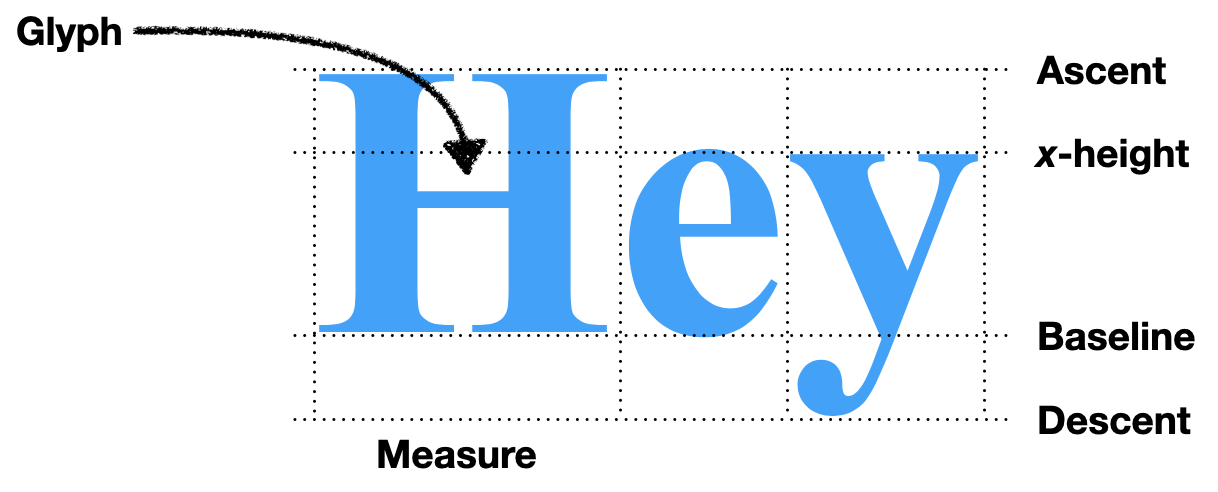
\includegraphics[width=0.8\textwidth]{im/text-metrics.jpg}
\caption{
The various vertical metrics of a font. All glyphs in
a font share the same ascent, $x$-height, and descent, and are laid
out on a shared baseline. However, the measure (or advance) of glyphs
can differ.}\label{fig:FontMetrics}
\end{figure}
% \end{center}

Let's dig deeper. Remember that \texttt{bi\_times} is size-16 Times: why
does \texttt{font.metrics} report that it is actually 19 pixels tall?
Well, first of all, a size of 16 means % sixteen
16~\emph{points}, which are
defined as 72nds of an inch, not % sixteen
16~\emph{pixels},\footnote{Actually, the definition of a ``point'' is a
  total mess, with many different length units all called ``point''
  around the world. The
  \href{https://en.wikipedia.org/wiki/Point_(typography)}{Wikipedia
  page} has the details, but a traditional American/British point is
  actually slightly less than 1/72 of an inch. The
  1/72 %\textsuperscript{nd}
  standard comes from PostScript, but some
  systems predate it; \TeX, for example, hews closer to the traditional
  point, approximating it as 1/72.27 %\textsuperscript{th}
  of an inch.}
which your monitor probably has around 100 of per inch.\footnote{Tk
  doesn't use points anywhere else in its API. It's supposed to use
  pixels if you pass it a negative number, but that doesn't appear to
  work.} Those % sixteen
16~points measure not the individual letters but the
metal blocks the letters were once carved from, so the letters
themselves must be \emph{less than} % sixteen
16~points. In fact, different
size-16 fonts have letters of varying heights:\footnote{You might even
  notice that Times has different metrics in this code block than in the
  earlier one where we specified a bold, italic Times font. The bold,
  italic Times font is taller, at least on my current macOS system!}
\begin{bookblock*}{notcode}
\begin{Shaded}
\begin{Highlighting}[]
\NormalTok{\textgreater{}\textgreater{}\textgreater{} tkinter.font.Font(family="Courier", size=16).metrics()}
\NormalTok{\{\textquotesingle{}fixed\textquotesingle{}: 1, \textquotesingle{}ascent\textquotesingle{}: 13, \textquotesingle{}descent\textquotesingle{}: 4, \textquotesingle{}linespace\textquotesingle{}: 17\}}
\NormalTok{\textgreater{}\textgreater{}\textgreater{} tkinter.font.Font(family="Times", size=16).metrics()}
\NormalTok{\{\textquotesingle{}fixed\textquotesingle{}: 0, \textquotesingle{}ascent\textquotesingle{}: 14, \textquotesingle{}descent\textquotesingle{}: 4, \textquotesingle{}linespace\textquotesingle{}: 18\}}
\NormalTok{\textgreater{}\textgreater{}\textgreater{} tkinter.font.Font(family="Helvetica", size=16).metrics()}
\NormalTok{\{\textquotesingle{}fixed\textquotesingle{}: 0, \textquotesingle{}ascent\textquotesingle{}: 15, \textquotesingle{}descent\textquotesingle{}: 4, \textquotesingle{}linespace\textquotesingle{}: 19\}}
\end{Highlighting}
\end{Shaded}
\end{bookblock*}

The \texttt{measure()} method is more direct: it tells you how much
\emph{horizontal} space text takes up, in pixels. This depends on the
text, of course, since different letters have different
widths:\footnote{Note that the sum of the individual letters' lengths is
  not the length of the word. Tk uses fractional pixels internally, but
  rounds up to return whole pixels in the \texttt{measure} call. Plus,
  some fonts use something called \emph{kerning} to shift letters a
  little bit when particular pairs of letters are next to one another,
  or even \emph{shaping} to make two letters look one glyph.}
\begin{bookblock*}{notcode}
\begin{Shaded}
\begin{Highlighting}[]
\NormalTok{\textgreater{}\textgreater{}\textgreater{} bi\_times.measure("Hi!")}
\NormalTok{24}
\NormalTok{\textgreater{}\textgreater{}\textgreater{} bi\_times.measure("H")}
\NormalTok{13}
\NormalTok{\textgreater{}\textgreater{}\textgreater{} bi\_times.measure("i")}
\NormalTok{5}
\NormalTok{\textgreater{}\textgreater{}\textgreater{} bi\_times.measure("!")}
\NormalTok{7}
\NormalTok{\textgreater{}\textgreater{}\textgreater{} 17 + 8 + 6}
\NormalTok{25}
\end{Highlighting}
\end{Shaded}
\end{bookblock*}

You can use this information to lay text out on the page. For example,
suppose you want to draw the text ``Hello, world!'' in two pieces, so
that ``world!'' is italic. Let's use two fonts:
\begin{Shaded}
\begin{Highlighting}[]
\NormalTok{font1 }\OperatorTok{=}\NormalTok{ tkinter.font.Font(family}\OperatorTok{=}\StringTok{"Times"}\NormalTok{, size}\OperatorTok{=}\DecValTok{16}\NormalTok{)}
\NormalTok{font2 }\OperatorTok{=}\NormalTok{ tkinter.font.Font(family}\OperatorTok{=}\StringTok{"Times"}\NormalTok{, size}\OperatorTok{=}\DecValTok{16}\NormalTok{, slant}\OperatorTok{=}\StringTok{\textquotesingle{}italic\textquotesingle{}}\NormalTok{)}
\end{Highlighting}
\end{Shaded}

We can now lay out the text, starting at \texttt{(200,\ 200)}:
\begin{Shaded}
\begin{Highlighting}[]
\NormalTok{x, y }\OperatorTok{=} \DecValTok{200}\NormalTok{, }\DecValTok{200}
\NormalTok{canvas.create\_text(x, y, text}\OperatorTok{=}\StringTok{"Hello, "}\NormalTok{, font}\OperatorTok{=}\NormalTok{font1)}
\NormalTok{x }\OperatorTok{+=}\NormalTok{ font1.measure(}\StringTok{"Hello, "}\NormalTok{)}
\NormalTok{canvas.create\_text(x, y, text}\OperatorTok{=}\StringTok{"world!"}\NormalTok{, font}\OperatorTok{=}\NormalTok{font2)}
\end{Highlighting}
\end{Shaded}
You should see ``Hello,'' and ``world!'', correctly aligned and with the
second word italicized.

Unfortunately, this code has a bug, though one masked by the choice of
example text: replace ``world!'' with ``overlapping!'' and the two words
will overlap. That's because the coordinates \texttt{x} and \texttt{y}
that you pass to \texttt{create\_text} tell Tk where to put the
\emph{center} of the text. It only worked for ``Hello, world!'' because
``Hello,'' and ``world!'' are the same length!

Luckily, the meaning of the coordinate you pass in is configurable. We
can instruct Tk to treat the coordinate we gave as the top-left corner
of the text by setting the \texttt{anchor} argument to \texttt{"nw"},
meaning the ``northwest'' corner of the text:
\begin{Shaded}
\begin{Highlighting}[]
\NormalTok{x, y }\OperatorTok{=} \DecValTok{200}\NormalTok{, }\DecValTok{225}
\NormalTok{canvas.create\_text(x, y, text}\OperatorTok{=}\StringTok{"Hello, "}\NormalTok{, font}\OperatorTok{=}\NormalTok{font1, anchor}\OperatorTok{=}\StringTok{\textquotesingle{}nw\textquotesingle{}}\NormalTok{)}
\NormalTok{x }\OperatorTok{+=}\NormalTok{ font1.measure(}\StringTok{"Hello, "}\NormalTok{)}
\NormalTok{canvas.create\_text(x, y, text}\OperatorTok{=}\StringTok{"overlapping!"}\NormalTok{, font}\OperatorTok{=}\NormalTok{font2, anchor}\OperatorTok{=}\StringTok{\textquotesingle{}nw\textquotesingle{}}\NormalTok{)}
\end{Highlighting}
\end{Shaded}
Modify the \texttt{draw} function to set \texttt{anchor} to
\texttt{"nw"}; we didn't need to do that in the previous chapter because
all Chinese characters are the same width.

\begin{bookblock}{further}
If you find font metrics confusing, you're not the only one! In 2012,
the Michigan Supreme Court heard
\href{https://publicdocs.courts.mi.gov/opinions/final/sct/20120803_s145387_157_standup-op.pdf}{Stand
Up for Democracy v.\ Secretary of State}, a case ultimately about a
ballot referendum's validity that centered on the definition of font
size. The court decided (correctly) that font size is the size of the
metal blocks that letters were carved from and not the size of the
letters themselves.
\end{bookblock}

\hypertarget{word-by-word}{%
\section{Word by Word}\label{word-by-word}}

In % the last
Chapter~\ref{ch:DrawingToTheScreen}, the \texttt{layout} function looped over the text
character by character and moved to the next line whenever we ran out of
space. That's appropriate in Chinese, where each character more or less
\emph{is} a word. But in English you can't move to the next line in the
middle of a word. Instead, we need to lay out the text one word at a
time:\footnote{This code splits words on whitespace. It'll thus break on
  Chinese, since there won't be whitespace between words. Real browsers
  use language-dependent rules for laying out text, including for
  identifying word boundaries.}
\begin{Shaded}
\begin{Highlighting}[]
\KeywordTok{def}\NormalTok{ layout(text):}
    \CommentTok{\# ...}
    \ControlFlowTok{for}\NormalTok{ word }\KeywordTok{in}\NormalTok{ text.split():}
        \CommentTok{\# ...}
    \ControlFlowTok{return}\NormalTok{ display\_list}
\end{Highlighting}
\end{Shaded}
Unlike Chinese characters, words are different sizes, so we need to
measure the width of each word:
\begin{Shaded}
\begin{Highlighting}[]
\KeywordTok{def}\NormalTok{ layout(text):}
\NormalTok{    font }\OperatorTok{=}\NormalTok{ tkinter.font.Font()}
    \CommentTok{\# ...}
    \ControlFlowTok{for}\NormalTok{ word }\KeywordTok{in}\NormalTok{ text.split():}
\NormalTok{        w }\OperatorTok{=}\NormalTok{ font.measure(word)}
    \CommentTok{\# ...}
\end{Highlighting}
\end{Shaded}
Here I've chosen to use Tk's default font. Now, if we draw the text at
\texttt{cursor\_x}, its right end would be at \texttt{cursor\_x\ +\ w}.
That might be past the right edge of the page, and in this case we need
to make space by wrapping to the next line:
\begin{Shaded}
\begin{Highlighting}[]
\KeywordTok{def}\NormalTok{ layout(text):}
    \ControlFlowTok{for}\NormalTok{ word }\KeywordTok{in}\NormalTok{ text.split():}
        \CommentTok{\# ...}
        \ControlFlowTok{if}\NormalTok{ cursor\_x }\OperatorTok{+}\NormalTok{ w }\OperatorTok{\textgreater{}}\NormalTok{ WIDTH }\OperatorTok{{-}}\NormalTok{ HSTEP:}
\NormalTok{            cursor\_y }\OperatorTok{+=}\NormalTok{ font.metrics(}\StringTok{"linespace"}\NormalTok{) }\OperatorTok{*} \FloatTok{1.25}
\NormalTok{            cursor\_x }\OperatorTok{=}\NormalTok{ HSTEP}
\end{Highlighting}
\end{Shaded}
Note that this code block only shows the insides of the \texttt{for}
loop. The rest of \texttt{layout} should be left alone. Also, I call
\texttt{metrics} with an argument; that just returns the named metric
directly. Finally, note that I multiply the linespace by 1.25 when
incrementing \texttt{y}. Try removing the multiplier: you'll see that
the text is harder to read because the lines are too close
together.\footnote{Designers say the text is too ``tight''.} Instead, it
is common to add ``line spacing'' or ``leading''\footnote{So named
  because in metal type days, thin pieces of lead were placed between
  the lines to space them out. Lead is a softer metal than what the
  actual letter pieces were made of, so it could compress a little to
  keep pressure on the other pieces. Pronounce it ``led-ing'' not
  ``leed-ing''.} between lines. The 25\% line spacing is a typical
amount.

So now \texttt{cursor\_x} and \texttt{cursor\_y} have the location to
\emph{start} drawing the word, so we add to the display list, and
finally we update \texttt{cursor\_x} to point to the end of the word:
\begin{Shaded}
\begin{Highlighting}[]
\KeywordTok{def}\NormalTok{ layout(text):}
    \ControlFlowTok{for}\NormalTok{ word }\KeywordTok{in}\NormalTok{ text.split():}
        \CommentTok{\# ...}
\NormalTok{        display\_list.append((cursor\_x, cursor\_y, word))}
\NormalTok{        cursor\_x }\OperatorTok{+=}\NormalTok{ w }\OperatorTok{+}\NormalTok{ font.measure(}\StringTok{" "}\NormalTok{)}
\end{Highlighting}
\end{Shaded}
I increment \texttt{cursor\_x} by \texttt{w\ +\ font.measure("\ ")}
instead of \texttt{w} because I want to have spaces between the words:
the call to \texttt{split()} removed all of the whitespace, and this
adds it back. I don't add the space to \texttt{w} in the \texttt{if}
condition, though, because you don't need a space after the last word on
a line.

\begin{bookblock}{further}
Breaking lines in the middle of a word is called hyphenation, and can be
turned on via the
\href{https://drafts.csswg.org/css-text-3/\#hyphens-property}{\texttt{hyphens}
CSS property}. The state of the art is the
\href{http://www.tug.org/docs/liang/liang-thesis.pdf}{Knuth--Liang
hyphenation algorithm}, which uses a dictionary of word fragments to
prioritize possible hyphenation points to implement this. At first, the
CSS specification
\href{https://news.ycombinator.com/item?id=19472922}{was incompatible}
with this algorithm, but the recent
\href{https://drafts.csswg.org/css-text-4/\#propdef-text-wrap-style}{\texttt{text-wrap-style}
property} fixed that.
\end{bookblock}

\hypertarget{styling-text}{%
\section{Styling Text}\label{styling-text}}

Right now, all of the text on the page is drawn with one font. But web
pages sometimes specify that text should be \textbf{bold} or \emph{italic} % text
using the
\texttt{\textless{}b\textgreater{}} and
\texttt{\textless{}i\textgreater{}} tags. It'd be nice to support that,
but right now, the code resists this: the \texttt{layout} function only
receives the text of the page as input, and so has no idea where the
bold and italics tags are.

Let's change \texttt{lex} to return a list of \emph{tokens}, where a
token is either a \texttt{Text} object (for a run of characters outside
a tag) or a \texttt{Tag} object (for the contents of a tag). You'll need
to write the \texttt{Text} and \texttt{Tag} classes:\footnote{If you're
  familiar with Python, you might want to use the \texttt{dataclass}
  library, which makes it easier to define these sorts of utility
  classes.}
\begin{Shaded}
\begin{Highlighting}[]
\KeywordTok{class}\NormalTok{ Text:}
    \KeywordTok{def} \FunctionTok{\_\_init\_\_}\NormalTok{(}\VariableTok{self}\NormalTok{, text):}
        \VariableTok{self}\NormalTok{.text }\OperatorTok{=}\NormalTok{ text}

\KeywordTok{class}\NormalTok{ Tag:}
    \KeywordTok{def} \FunctionTok{\_\_init\_\_}\NormalTok{(}\VariableTok{self}\NormalTok{, tag):}
        \VariableTok{self}\NormalTok{.tag }\OperatorTok{=}\NormalTok{ tag}
\end{Highlighting}
\end{Shaded}

\texttt{lex} must now gather text into \texttt{Text} and \texttt{Tag}
objects:\footnote{If you've done some or all of the exercises in prior chapters, your code
  will look different. Code snippets in the book always assume you
  haven't done the exercises, so you'll need to port your modifications.}
\begin{Shaded}
\begin{Highlighting}[]
\KeywordTok{def}\NormalTok{ lex(body):}
\NormalTok{    out }\OperatorTok{=}\NormalTok{ []}
    \BuiltInTok{buffer} \OperatorTok{=} \StringTok{""}
\NormalTok{    in\_tag }\OperatorTok{=} \VariableTok{False}
    \ControlFlowTok{for}\NormalTok{ c }\KeywordTok{in}\NormalTok{ body:}
        \ControlFlowTok{if}\NormalTok{ c }\OperatorTok{==} \StringTok{"\textless{}"}\NormalTok{:}
\NormalTok{            in\_tag }\OperatorTok{=} \VariableTok{True}
            \ControlFlowTok{if} \BuiltInTok{buffer}\NormalTok{: out.append(Text(}\BuiltInTok{buffer}\NormalTok{))}
            \BuiltInTok{buffer} \OperatorTok{=} \StringTok{""}
        \ControlFlowTok{elif}\NormalTok{ c }\OperatorTok{==} \StringTok{"\textgreater{}"}\NormalTok{:}
\NormalTok{            in\_tag }\OperatorTok{=} \VariableTok{False}
\NormalTok{            out.append(Tag(}\BuiltInTok{buffer}\NormalTok{))}
            \BuiltInTok{buffer} \OperatorTok{=} \StringTok{""}
        \ControlFlowTok{else}\NormalTok{:}
            \BuiltInTok{buffer} \OperatorTok{+=}\NormalTok{ c}
    \ControlFlowTok{if} \KeywordTok{not}\NormalTok{ in\_tag }\KeywordTok{and} \BuiltInTok{buffer}\NormalTok{:}
\NormalTok{        out.append(Text(}\BuiltInTok{buffer}\NormalTok{))}
    \ControlFlowTok{return}\NormalTok{ out}
\end{Highlighting}
\end{Shaded}
Here I've renamed the \texttt{text} variable to \texttt{buffer}, since
it now stores either text or tag contents before they can be used. The
name also reminds us that, at the end of the loop, we need to check
whether there's buffered text and what we should do with it. Here,
\texttt{lex} dumps any accumulated text as a \texttt{Text} object.
Otherwise, if you never saw an angle bracket, you'd return an empty list
of tokens. But unfinished tags, like in \texttt{Hi!\textless{}hr}, are
thrown out.\footnote{This may strike you as an odd decision: why not
  raise an error, or finish up the tag for the author? I don't know, but
  dropping the tag is what browsers do.}

Note that \texttt{Text} and \texttt{Tag} are asymmetric: \texttt{lex}
avoids empty \texttt{Text} objects, but not empty \texttt{Tag} objects.
That's because an empty \texttt{Tag} object represents the HTML code
\texttt{\textless{}\textgreater{}}, while an empty \texttt{Text} object
with empty text represents no content at all.

Since we've modified \texttt{lex} we are now passing \texttt{layout} not
just the text of the page, but also the tags in it. So \texttt{layout}
must loop over tokens, not text:
\begin{Shaded}
\begin{Highlighting}[]
\KeywordTok{def}\NormalTok{ layout(tokens):}
    \CommentTok{\# ...}
    \ControlFlowTok{for}\NormalTok{ tok }\KeywordTok{in}\NormalTok{ tokens:}
        \ControlFlowTok{if} \BuiltInTok{isinstance}\NormalTok{(tok, Text):}
            \ControlFlowTok{for}\NormalTok{ word }\KeywordTok{in}\NormalTok{ tok.text.split():}
                \CommentTok{\# ...}
    \CommentTok{\# ...}
\end{Highlighting}
\end{Shaded}

\texttt{layout} can also examine tag tokens to change font when directed
by the page. Let's start with support for weights and styles, with two
corresponding variables:
\begin{Shaded}
\begin{Highlighting}[]
\NormalTok{weight }\OperatorTok{=} \StringTok{"normal"}
\NormalTok{style }\OperatorTok{=} \StringTok{"roman"}
\end{Highlighting}
\end{Shaded}
Those variables must change when the bold and italics open and close
tags are seen:
\begin{Shaded}
\begin{Highlighting}[]
\ControlFlowTok{if} \BuiltInTok{isinstance}\NormalTok{(tok, Text):}
    \CommentTok{\# ...}
\ControlFlowTok{elif}\NormalTok{ tok.tag }\OperatorTok{==} \StringTok{"i"}\NormalTok{:}
\NormalTok{    style }\OperatorTok{=} \StringTok{"italic"}
\ControlFlowTok{elif}\NormalTok{ tok.tag }\OperatorTok{==} \StringTok{"/i"}\NormalTok{:}
\NormalTok{    style }\OperatorTok{=} \StringTok{"roman"}
\ControlFlowTok{elif}\NormalTok{ tok.tag }\OperatorTok{==} \StringTok{"b"}\NormalTok{:}
\NormalTok{    weight }\OperatorTok{=} \StringTok{"bold"}
\ControlFlowTok{elif}\NormalTok{ tok.tag }\OperatorTok{==} \StringTok{"/b"}\NormalTok{:}
\NormalTok{    weight }\OperatorTok{=} \StringTok{"normal"}
\end{Highlighting}
\end{Shaded}
Note that this code correctly handles not only
\texttt{\textless{}b\textgreater{}bold\textless{}/b\textgreater{}} and
\texttt{\textless{}i\textgreater{}italic\textless{}/i\textgreater{}}
text, but also
\texttt{\textless{}b\textgreater{}\textless{}i\textgreater{}bold\ italic\textless{}/i\textgreater{}\textless{}/b\textgreater{}}
text.\footnote{It even handles % mis-
  incorrectly nested tags like
  \texttt{\textless{}b\textgreater{}b\textless{}i\textgreater{}bi\textless{}/b\textgreater{}i\textless{}/i\textgreater{}},
  but it does not handle
  \texttt{\textless{}b\textgreater{}\textless{}b\textgreater{}twice\textless{}/b\textgreater{}bolded\textless{}/b\textgreater{}}
  text. We'll return to this in  %\href{styles.md}{a later
  Chapter~\ref{ch:ApplyingAuthorStyles}.}

The \texttt{bold} and \texttt{italic} variables are used to select the
font:
\begin{Shaded}
\begin{Highlighting}[]
\ControlFlowTok{if} \BuiltInTok{isinstance}\NormalTok{(tok, Text):}
    \ControlFlowTok{for}\NormalTok{ word }\KeywordTok{in}\NormalTok{ tok.text.split():}
\NormalTok{        font }\OperatorTok{=}\NormalTok{ tkinter.font.Font(}
\NormalTok{            size}\OperatorTok{=}\DecValTok{16}\NormalTok{,}
\NormalTok{            weight}\OperatorTok{=}\NormalTok{weight,}
\NormalTok{            slant}\OperatorTok{=}\NormalTok{style,}
\NormalTok{        )}
        \CommentTok{\# ...}
\end{Highlighting}
\end{Shaded}

Since the font is computed in \texttt{layout} but used in \texttt{draw},
we'll need to add the font used to each entry in the display list:
\begin{Shaded}
\begin{Highlighting}[]
\ControlFlowTok{if} \BuiltInTok{isinstance}\NormalTok{(tok, Text):}
    \ControlFlowTok{for}\NormalTok{ word }\KeywordTok{in}\NormalTok{ tok.text.split():}
        \CommentTok{\# ...}
\NormalTok{        display\_list.append((cursor\_x, cursor\_y, word, font))}
\end{Highlighting}
\end{Shaded}
Make sure to update \texttt{draw} to expect and use this extra font
field in display list entries.

\begin{bookblock}{further}
\emph{Italic} fonts were developed in Italy (hence the name) to mimic a
cursive handwriting style called
``\href{https://en.wikipedia.org/wiki/Chancery_hand}{chancery hand}''.
Non-italic fonts are called \emph{roman} because they mimic text on
Roman monuments. There is an obscure third option:
\href{https://en.wikipedia.org/wiki/Oblique_type}{\textsl{oblique} fonts},
which look like roman fonts but are slanted.
\end{bookblock}

\hypertarget{a-layout-object}{%
\section{A Layout Object}\label{a-layout-object}}

With all of these tags, \texttt{layout} has become quite large, with
lots of local variables and some complicated control flow. That is one
sign that something deserves to be a class, not a function:
\begin{Shaded}
\begin{Highlighting}[]
\KeywordTok{class}\NormalTok{ Layout:}
    \KeywordTok{def} \FunctionTok{\_\_init\_\_}\NormalTok{(}\VariableTok{self}\NormalTok{, tokens):}
        \VariableTok{self}\NormalTok{.display\_list }\OperatorTok{=}\NormalTok{ []}
\end{Highlighting}
\end{Shaded}
Every local variable in \texttt{layout} then becomes a field of
\texttt{Layout}:
\begin{Shaded}
\begin{Highlighting}[]
\VariableTok{self}\NormalTok{.cursor\_x }\OperatorTok{=}\NormalTok{ HSTEP}
\VariableTok{self}\NormalTok{.cursor\_y }\OperatorTok{=}\NormalTok{ VSTEP}
\VariableTok{self}\NormalTok{.weight }\OperatorTok{=} \StringTok{"normal"}
\VariableTok{self}\NormalTok{.style }\OperatorTok{=} \StringTok{"roman"}
\VariableTok{self}\NormalTok{.size }\OperatorTok{=} \DecValTok{16}
\end{Highlighting}
\end{Shaded}

The core of the old \texttt{layout} is a loop over tokens, and we can
move the body of that loop to a method on \texttt{Layout}:
\begin{Shaded}
\begin{Highlighting}[]
\KeywordTok{def} \FunctionTok{\_\_init\_\_}\NormalTok{(}\VariableTok{self}\NormalTok{, tokens):}
    \CommentTok{\# ...}
    \ControlFlowTok{for}\NormalTok{ tok }\KeywordTok{in}\NormalTok{ tokens:}
        \VariableTok{self}\NormalTok{.token(tok)}

\KeywordTok{def}\NormalTok{ token(}\VariableTok{self}\NormalTok{, tok):}
    \ControlFlowTok{if} \BuiltInTok{isinstance}\NormalTok{(tok, Text):}
        \ControlFlowTok{for}\NormalTok{ word }\KeywordTok{in}\NormalTok{ tok.text.split():}
            \CommentTok{\# ...}
    \ControlFlowTok{elif}\NormalTok{ tok.tag }\OperatorTok{==} \StringTok{"i"}\NormalTok{:}
        \VariableTok{self}\NormalTok{.style }\OperatorTok{=} \StringTok{"italic"}
    \CommentTok{\# ...}
\end{Highlighting}
\end{Shaded}
In fact, the body of the \texttt{isinstance(tok,\ Text)} branch can be
moved to its own method:
\begin{Shaded}
\begin{Highlighting}[]
\KeywordTok{def}\NormalTok{ word(}\VariableTok{self}\NormalTok{, word):}
\NormalTok{    font }\OperatorTok{=}\NormalTok{ tkinter.font.Font(}
\NormalTok{        size}\OperatorTok{=}\DecValTok{16}\NormalTok{,}
\NormalTok{        weight}\OperatorTok{=}\VariableTok{self}\NormalTok{.weight,}
\NormalTok{        slant}\OperatorTok{=}\VariableTok{self}\NormalTok{.style,}
\NormalTok{    )}
\NormalTok{    w }\OperatorTok{=}\NormalTok{ font.measure(word)}
    \CommentTok{\# ...}
\end{Highlighting}
\end{Shaded}

Now that everything has moved out of \texttt{Browser}'s old
\texttt{layout} function, it can be replaced with calls into
\texttt{Layout}:
\begin{Shaded}
\begin{Highlighting}[]
\KeywordTok{class}\NormalTok{ Browser:}
    \KeywordTok{def}\NormalTok{ load(}\VariableTok{self}\NormalTok{, url):}
\NormalTok{        body }\OperatorTok{=}\NormalTok{ url.request()}
\NormalTok{        tokens }\OperatorTok{=}\NormalTok{ lex(body)}
        \VariableTok{self}\NormalTok{.display\_list }\OperatorTok{=}\NormalTok{ Layout(tokens).display\_list}
        \VariableTok{self}\NormalTok{.draw()}
\end{Highlighting}
\end{Shaded}

When you do big refactors like this, it's important to work
incrementally. It might seem more efficient to change everything at
once, but that efficiency brings with it a risk of failure: trying to do so
much that you get confused and have to abandon the whole refactor. So
take a moment to test that your browser still works before you move on.

Anyway, this refactor isolated all of the text-handling code into its
own method, with the main \texttt{token} function just branching on the
tag name. Let's take advantage of the new, cleaner organization to add
more tags. With font weights and styles working, size is the next
frontier in typographic sophistication. One simple way to change font
size is the \texttt{\textless{}small\textgreater{}} tag and its
deprecated sister tag \texttt{\textless{}big\textgreater{}}.\footnote{In
  your web design projects, use the CSS \texttt{font-size} property to
  change text size instead of \texttt{\textless{}big\textgreater{}} and
  \texttt{\textless{}small\textgreater{}}. But since we haven't yet
%  \href{styles.html}{
  implemented CSS for our browser (see Chapter~\ref{ch:ApplyingAuthorStyles}), we're stuck using
  them here.}

Our experience with font styles and weights suggests a simple approach
that customizes the \texttt{size} field in \texttt{Layout}. It starts out as:
\begin{Shaded}
\begin{Highlighting}[]
\VariableTok{self}\NormalTok{.size }\OperatorTok{=} \DecValTok{12}
\end{Highlighting}
\end{Shaded}
That variable is used to create the font object:
\begin{Shaded}
\begin{Highlighting}[]
\NormalTok{font }\OperatorTok{=}\NormalTok{ tkinter.font.Font(}
\NormalTok{    size}\OperatorTok{=}\VariableTok{self}\NormalTok{.size,}
\NormalTok{    weight}\OperatorTok{=}\VariableTok{self}\NormalTok{.weight,}
\NormalTok{    slant}\OperatorTok{=}\VariableTok{self}\NormalTok{.style,}
\NormalTok{)}
\end{Highlighting}
\end{Shaded}
And so we can change the sizes of \texttt{\textless{}big\textgreater{}} and
\texttt{\textless{}small\textgreater{}} tags by updating this variable:
\begin{Shaded}
\begin{Highlighting}[]
\KeywordTok{def}\NormalTok{ token(}\VariableTok{self}\NormalTok{, tok):}
    \CommentTok{\# ...}
    \ControlFlowTok{elif}\NormalTok{ tok.tag }\OperatorTok{==} \StringTok{"small"}\NormalTok{:}
        \VariableTok{self}\NormalTok{.size }\OperatorTok{{-}=} \DecValTok{2}
    \ControlFlowTok{elif}\NormalTok{ tok.tag }\OperatorTok{==} \StringTok{"/small"}\NormalTok{:}
        \VariableTok{self}\NormalTok{.size }\OperatorTok{+=} \DecValTok{2}
    \ControlFlowTok{elif}\NormalTok{ tok.tag }\OperatorTok{==} \StringTok{"big"}\NormalTok{:}
        \VariableTok{self}\NormalTok{.size }\OperatorTok{+=} \DecValTok{4}
    \ControlFlowTok{elif}\NormalTok{ tok.tag }\OperatorTok{==} \StringTok{"/big"}\NormalTok{:}
        \VariableTok{self}\NormalTok{.size }\OperatorTok{{-}=} \DecValTok{4}
\end{Highlighting}
\end{Shaded}

Try wrapping a whole paragraph in
\texttt{\textless{}small\textgreater{}}, like you would a bit of fine
print, and enjoy your newfound typographical freedom.

\begin{bookblock}{further}
All of \texttt{\textless{}b\textgreater{}},
\texttt{\textless{}i\textgreater{}},
\texttt{\textless{}big\textgreater{}}, and
\texttt{\textless{}small\textgreater{}} date from an earlier, pre-CSS
era of the web. Nowadays, CSS can change how an element appears, so
visual tag names like \texttt{\textless{}b\textgreater{}} and
\texttt{\textless{}small\textgreater{}} are out of favor. That said,
\texttt{\textless{}b\textgreater{}},
\texttt{\textless{}i\textgreater{}}, and
\texttt{\textless{}small\textgreater{}} still have some
\href{https://html.spec.whatwg.org/multipage/text-level-semantics.html\#the-small-element}{appearance-independent
meanings}.
\end{bookblock}

\hypertarget{text-of-different-sizes}{%
\section{Text of Different Sizes}\label{text-of-different-sizes}}

Start mixing font sizes, like
\texttt{\textless{}small\textgreater{}a\textless{}/small\textgreater{}\textless{}big\textgreater{}A\textless{}/big\textgreater{}},
and you'll quickly notice a problem with the font size code: the text is
aligned along its top, as if it's hanging from a clothes line. But you
know that English text is typically written with all letters aligned at
an invisible \emph{baseline} instead.

Let's think through how to fix this. If the big text is moved up, it
would overlap with the previous line, so the smaller text has to be
moved down. That means its vertical position has to be computed later,
\emph{after} the big text passes through \texttt{token}. But since the
small text comes through the loop first, we need a \emph{two-pass}
algorithm for lines of text: the first pass identifies what words go in
the line and computes their $x$ positions, while the second pass
vertically aligns the words and computes their $y$ positions (see Figure~\ref{fig:MultipleFonts}).

%\begin{center}
\begin{figure}
  \centering
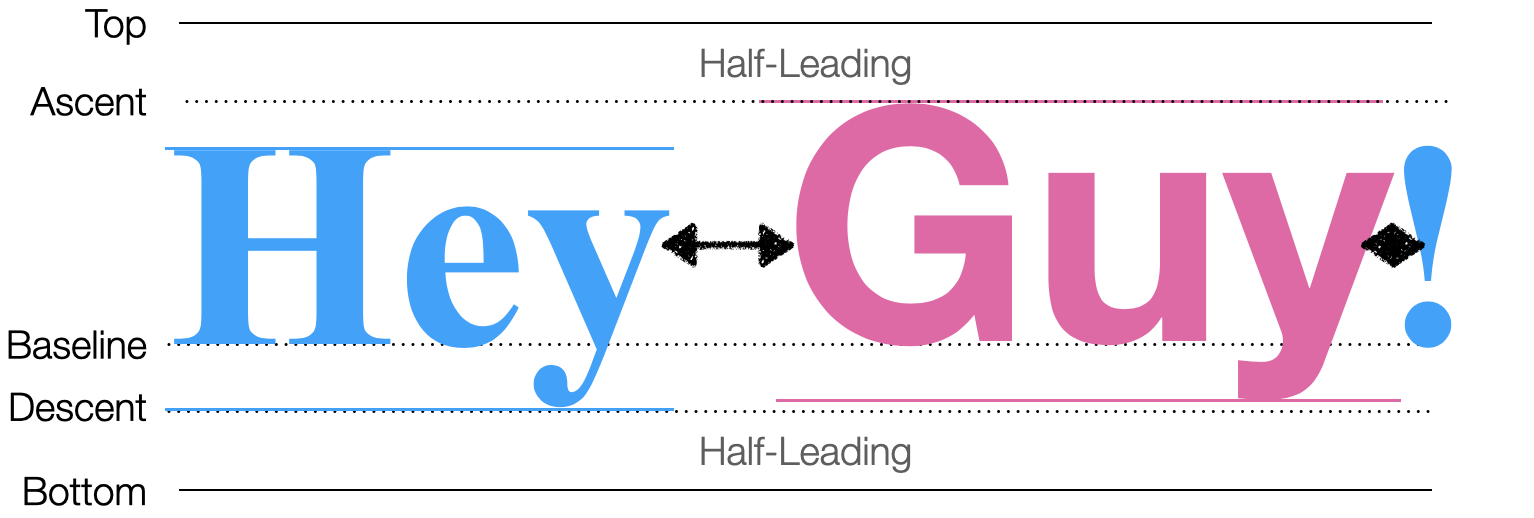
\includegraphics[width=0.9\textwidth]{im/text-line.jpg}
\caption{How lines are laid out when multiple fonts are
involved. All words are drawn using a shared baseline. The ascent and
descent of the whole line is then determined by the maximum ascent and
descent of all words in the line, and leading is added before and after
the line.}
\label{fig:MultipleFonts}
\end{figure}
% \end{center}

Let's start with phase one. Since one line contains text from many tags,
we need a field on \texttt{Layout} to store the line-to-be. That field,
\texttt{line}, will be a list, and \texttt{text} will add words to it
instead of to the display list. Entries in \texttt{line} will have
$x$ but not $y$ positions, since $y$ positions aren't
computed in the first phase:
\begin{Shaded}
\begin{Highlighting}[]
\KeywordTok{class}\NormalTok{ Layout:}
    \KeywordTok{def} \FunctionTok{\_\_init\_\_}\NormalTok{(}\VariableTok{self}\NormalTok{, tokens):}
        \CommentTok{\# ...}
        \VariableTok{self}\NormalTok{.line }\OperatorTok{=}\NormalTok{ []}
        \CommentTok{\# ...}
    
    \KeywordTok{def}\NormalTok{ word(}\VariableTok{self}\NormalTok{, word):}
        \CommentTok{\# ...}
        \VariableTok{self}\NormalTok{.line.append((}\VariableTok{self}\NormalTok{.cursor\_x, word, font))}
\end{Highlighting}
\end{Shaded}

The new \texttt{line} field is essentially a buffer, where words are
held temporarily before they can be placed. The second phase is that
buffer being flushed when we're finished with a line:
\begin{Shaded}
\begin{Highlighting}[]
\KeywordTok{class}\NormalTok{ Layout:}
    \KeywordTok{def}\NormalTok{ word(}\VariableTok{self}\NormalTok{, word):}
        \ControlFlowTok{if} \VariableTok{self}\NormalTok{.cursor\_x }\OperatorTok{+}\NormalTok{ w }\OperatorTok{\textgreater{}}\NormalTok{ WIDTH }\OperatorTok{{-}}\NormalTok{ HSTEP:}
            \VariableTok{self}\NormalTok{.flush()}
\end{Highlighting}
\end{Shaded}

As usual with buffers, we also need to make sure the buffer is flushed
once all tokens are processed:
\begin{Shaded}
\begin{Highlighting}[]
\KeywordTok{class}\NormalTok{ Layout:}
    \KeywordTok{def} \FunctionTok{\_\_init\_\_}\NormalTok{(}\VariableTok{self}\NormalTok{, tokens):}
        \CommentTok{\# ...}
        \VariableTok{self}\NormalTok{.flush()}
\end{Highlighting}
\end{Shaded}
This new \texttt{flush} function has three responsibilities:
\begin{itemize}
%\def\labelenumi{\arabic{enumi}.}
\tightlist
\item it must align the words along the baseline (see Figure~\ref{fig:AlignWords});
\item it must add all those words to the display list; and
\item it must update the \texttt{cursor\_x} and \texttt{cursor\_y} fields.
\end{itemize}

%\begin{center}

\begin{figure}[b!]
\centering
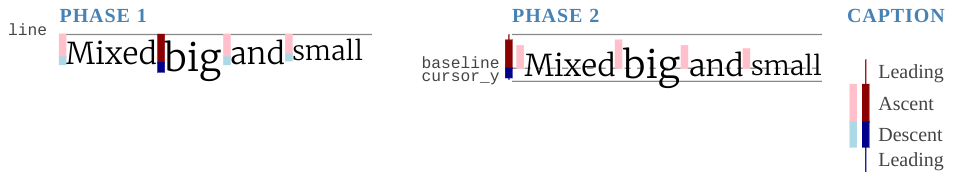
\includegraphics{examples/example3-words-align.png}
\caption{Aligning the words on a line.}\label{fig:AlignWords}
\end{figure}

%\end{center}

Since we want words to line up ``on the line'', let's start by computing
where that line should be. That depends on the tallest word on the line:
\begin{Shaded}
\begin{Highlighting}[]
\KeywordTok{def}\NormalTok{ flush(}\VariableTok{self}\NormalTok{):}
    \ControlFlowTok{if} \KeywordTok{not} \VariableTok{self}\NormalTok{.line: }\ControlFlowTok{return}
\NormalTok{    max\_ascent }\OperatorTok{=} \BuiltInTok{max}\NormalTok{([font.metrics(}\StringTok{"ascent"}\NormalTok{)}
        \ControlFlowTok{for}\NormalTok{ x, word, font }\KeywordTok{in} \VariableTok{self}\NormalTok{.line])}
\end{Highlighting}
\end{Shaded}
The line is then \texttt{max\_ascent} below \texttt{self.y}---or
actually a little more to account for the leading:\footnote{Actually,
  25\% leading doesn't add 25\% of the ascent above the ascender and
  25\% of the descent below the descender. Instead, it adds
  \href{https://www.w3.org/TR/CSS2/visudet.html\#leading}{12.5\% of the
  line height in both places}, which is subtly different when fonts are
  mixed. But let's skip that subtlety here.}
\begin{Shaded}
\begin{Highlighting}[]
\NormalTok{baseline }\OperatorTok{=} \VariableTok{self}\NormalTok{.cursor\_y }\OperatorTok{+} \FloatTok{1.25} \OperatorTok{*}\NormalTok{ max\_ascent}
\end{Highlighting}
\end{Shaded}

Now that we know where the line is, we can place each word relative to
that line and add it to the display list:
\begin{Shaded}
\begin{Highlighting}[]
\ControlFlowTok{for}\NormalTok{ x, word, font }\KeywordTok{in} \VariableTok{self}\NormalTok{.line:}
\NormalTok{    y }\OperatorTok{=}\NormalTok{ baseline }\OperatorTok{{-}}\NormalTok{ font.metrics(}\StringTok{"ascent"}\NormalTok{)}
    \VariableTok{self}\NormalTok{.display\_list.append((x, y, word, font))}
\end{Highlighting}
\end{Shaded}
Note how \texttt{y} starts at the baseline, and moves \emph{up} by just
enough to accommodate that word's ascent. Now \texttt{y} must move far
enough down below \texttt{baseline} to account for the deepest
descender:
\begin{Shaded}
\begin{Highlighting}[]
\NormalTok{max\_descent }\OperatorTok{=} \BuiltInTok{max}\NormalTok{([metric[}\StringTok{"descent"}\NormalTok{] }\ControlFlowTok{for}\NormalTok{ metric }\KeywordTok{in}\NormalTok{ metrics])}
\VariableTok{self}\NormalTok{.cursor\_y }\OperatorTok{=}\NormalTok{ baseline }\OperatorTok{+} \FloatTok{1.25} \OperatorTok{*}\NormalTok{ max\_descent}
\end{Highlighting}
\end{Shaded}

Finally, \texttt{flush} must update the \texttt{Layout}'s \texttt{x},
\texttt{y}, and \texttt{line} fields. \texttt{x} and \texttt{line} are
easy:
\begin{Shaded}
\begin{Highlighting}[]
\VariableTok{self}\NormalTok{.cursor\_x }\OperatorTok{=}\NormalTok{ HSTEP}
\VariableTok{self}\NormalTok{.line }\OperatorTok{=}\NormalTok{ []}
\end{Highlighting}
\end{Shaded}

Now all the text is aligned along the line, even when text sizes are
mixed. Plus, this new \texttt{flush} function is convenient for other
line-breaking jobs. For example, in HTML the
\texttt{\textless{}br\textgreater{}} tag\footnote{Which is a
  self-closing tag, so there's no \texttt{\textless{}/br\textgreater{}}.
  Many tags that \emph{are} content, instead of annotating it, are like
  this. Some people like adding a final slash to self-closing tags, as
  in \texttt{\textless{}br/\textgreater{}}, but this is not required in
  HTML.} ends the current line and starts a new one:
\begin{Shaded}
\begin{Highlighting}[]
\KeywordTok{def}\NormalTok{ token(}\VariableTok{self}\NormalTok{, tok):}
    \CommentTok{\# ...}
    \ControlFlowTok{elif}\NormalTok{ tok.tag }\OperatorTok{==} \StringTok{"br"}\NormalTok{:}
        \VariableTok{self}\NormalTok{.flush()}
\end{Highlighting}
\end{Shaded}

Likewise, paragraphs are defined by the
\texttt{\textless{}p\textgreater{}} and
\texttt{\textless{}/p\textgreater{}} tags, so
\texttt{\textless{}/p\textgreater{}} also ends the current line:
\begin{Shaded}
\begin{Highlighting}[]
\KeywordTok{def}\NormalTok{ token(}\VariableTok{self}\NormalTok{, tok):}
    \CommentTok{\# ...}
    \ControlFlowTok{elif}\NormalTok{ tok.tag }\OperatorTok{==} \StringTok{"/p"}\NormalTok{:}
        \VariableTok{self}\NormalTok{.flush()}
        \VariableTok{self}\NormalTok{.cursor\_y }\OperatorTok{+=}\NormalTok{ VSTEP}
\end{Highlighting}
\end{Shaded}
I add a bit extra to \texttt{cursor\_y} here to create a little gap
between paragraphs.

By this point you should be able to load up your browser and display
\href{https://browser.engineering/examples/example3-sizes.html}{this page}, %. It
which should look % about
something like Figure~\ref{fig:TextSizes}. %this:

% \begin{center}

\begin{figure}[b!]
\centering
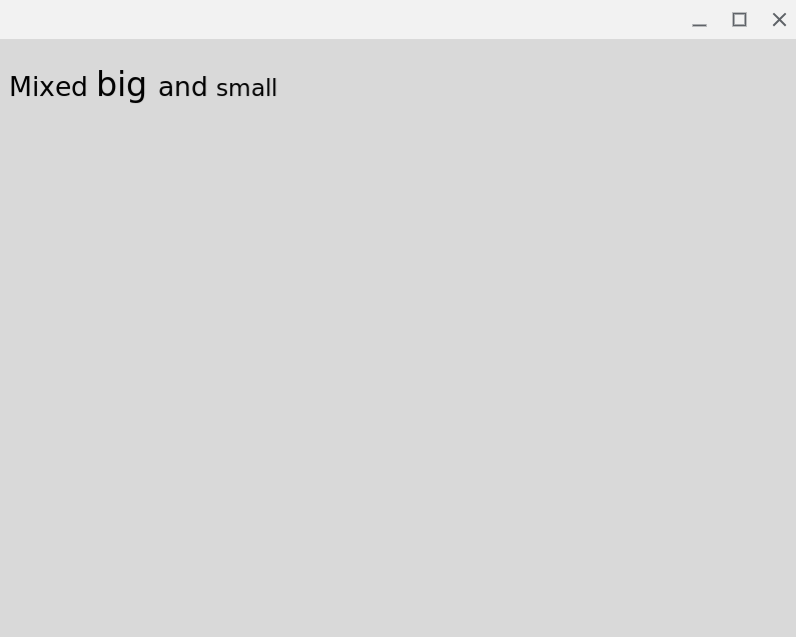
\includegraphics[width=0.8\textwidth]{examples/example3-sizes-screenshot.png}
\caption{Screenshot of a web page demonstrating different text sizes.}\label{fig:TextSizes}
\end{figure}

%\end{center}

\begin{bookblock}{further}
Actually, browsers support not only \emph{horizontal} but also
\href{https://www.smashingmagazine.com/2019/08/writing-modes-layout/}{\emph{vertical}
writing systems}, like some traditional East Asian writing styles. A
particular challenge is \href{https://www.w3.org/TR/mlreq/}{Mongolian
script}, which is written in lines running top to bottom, left to right.
Many Mongolian \href{https://president.mn/mng/}{government websites} use
the script.
\end{bookblock}

\hypertarget{font-caching}{%
\section{Font caching}\label{font-caching}}

Now that you've implemented styled text, you've probably
noticed---unless you're on macOS\footnote{While we can't confirm this in
  the documentation, it seems that the macOS ``Core Text'' APIs cache
  fonts more aggressively than Linux and Windows. The optimization
  described in this section won't hurt any on macOS, but also won't
  improve speed as much as on Windows and Linux.}---that on a large web
page like \href{https://browser.engineering/text.html}{this chapter}
our browser has slowed significantly from the
{previous chapter}. That's because text layout, and
specifically the part where you measure each word, is quite
slow.\footnote{You can profile Python programs by replacing your
  \texttt{python3} command with \texttt{python3\ -m\ cProfile}. Look for
  the lines corresponding to the \texttt{measure} and \texttt{metrics}
  calls to see how much time is spent measuring text.}

Unfortunately, it's hard to make text measurement much faster. With
proportional fonts and complex font features like hinting and kerning,
measuring text can require pretty complex computations. But on a large
web page, some words likely appear a lot---for example, this page
includes the word ``the'' over % two hundred
200 times. Instead of measuring
these words over and over again, we could measure them once, and then
cache the results. On normal English text, this usually results in a
substantial speedup.

Caching is such a good idea that most text libraries already implement
it, typically caching text measurements in each \texttt{Font} object.
But since our \texttt{text} method creates a new \texttt{Font} object
for each word, the caching is ineffective. To make caching work, we need
to reuse \texttt{Font} objects when possible instead of making new ones.

We'll store our cache in a global \texttt{FONTS} dictionary:
\begin{Shaded}
\begin{Highlighting}[]
\NormalTok{FONTS }\OperatorTok{=}\NormalTok{ \{\}}
\end{Highlighting}
\end{Shaded}
The keys to this dictionary will be size/weight/style triples, and the
values will be \texttt{Font} objects.\footnote{Actually, the values are
  a font object and a \texttt{tkinter.Label} object. This dramatically
  improves the performance of \texttt{metrics} for some reason, and is
  recommended by the
  \href{https://github.com/python/cpython/blob/main/Lib/tkinter/font.py\#L163}{Python
  documentation}.} We can put the caching logic itself in a new
\texttt{get\_font} function:
\begin{Shaded}
\begin{Highlighting}[]
\KeywordTok{def}\NormalTok{ get\_font(size, weight, style):}
\NormalTok{    key }\OperatorTok{=}\NormalTok{ (size, weight, style)}
    \ControlFlowTok{if}\NormalTok{ key }\KeywordTok{not} \KeywordTok{in}\NormalTok{ FONTS:}
\NormalTok{        font }\OperatorTok{=}\NormalTok{ tkinter.font.Font(size}\OperatorTok{=}\NormalTok{size, weight}\OperatorTok{=}\NormalTok{weight,}
\NormalTok{            slant}\OperatorTok{=}\NormalTok{style)}
\NormalTok{        label }\OperatorTok{=}\NormalTok{ tkinter.Label(font}\OperatorTok{=}\NormalTok{font)}
\NormalTok{        FONTS[key] }\OperatorTok{=}\NormalTok{ (font, label)}
    \ControlFlowTok{return}\NormalTok{ FONTS[key][}\DecValTok{0}\NormalTok{]}
\end{Highlighting}
\end{Shaded}
Then the \texttt{word} method can call \texttt{get\_font} instead of
creating a \texttt{Font} object directly:
\begin{Shaded}
\begin{Highlighting}[]
\KeywordTok{class}\NormalTok{ Layout:}
    \KeywordTok{def}\NormalTok{ word(}\VariableTok{self}\NormalTok{, word):}
\NormalTok{        font }\OperatorTok{=}\NormalTok{ get\_font(}\VariableTok{self}\NormalTok{.size, }\VariableTok{self}\NormalTok{.weight, }\VariableTok{self}\NormalTok{.style)}
        \CommentTok{\# ...}
\end{Highlighting}
\end{Shaded}
Now identical words will use identical fonts and text measurements will
hit the cache.

\begin{bookblock}{further}
Fonts for scripts like Chinese can be megabytes in size, so they are
generally stored on disk and only loaded into memory on demand. That
makes font loading slow and caching even more important. Browsers also
have extensive caches for measuring, shaping, and rendering text.
Because web pages have a lot of text, these caches turn out to be one of
the most important parts of speeding up rendering.
\end{bookblock}

\hypertarget{summary}{%
\section{Summary}\label{FormattingText-summary}}

The % last
previous chapter introduced a browser that laid out characters in a
grid. Now it does standard English text layout, so:
\begin{itemize}
\tightlist
\item
  text is laid out word by word;
\item
  lines are split at word boundaries;
\item
  text can be bold or italic;
\item
  text of different sizes can be mixed.
\end{itemize}
You can now use our browser to read an essay, a blog post, or even a
book!

\hypertarget{outline}{%
\section{Outline}\label{FormattingText-outline}}

The complete set of functions, classes, and methods in our browser
should look something like this:
\begin{Shaded}
\begin{Highlighting}[]
\KeywordTok{class}\NormalTok{ URL:}
    \KeywordTok{def} \FunctionTok{\_\_init\_\_}\NormalTok{(url)}
    \KeywordTok{def}\NormalTok{ request()}
\NormalTok{WIDTH}
\NormalTok{HEIGHT}
\NormalTok{HSTEP}
\NormalTok{VSTEP}
\NormalTok{SCROLL\_STEP}
\KeywordTok{class}\NormalTok{ Browser:}
    \KeywordTok{def} \FunctionTok{\_\_init\_\_}\NormalTok{()}
    \KeywordTok{def}\NormalTok{ load(url)}
    \KeywordTok{def}\NormalTok{ draw()}
    \KeywordTok{def}\NormalTok{ scrolldown(e)}
\KeywordTok{class}\NormalTok{ Text:}
    \KeywordTok{def} \FunctionTok{\_\_init\_\_}\NormalTok{(text)}
\KeywordTok{class}\NormalTok{ Tag:}
    \KeywordTok{def} \FunctionTok{\_\_init\_\_}\NormalTok{(tag)}
\KeywordTok{def}\NormalTok{ lex(body)}
\NormalTok{FONTS}
\KeywordTok{def}\NormalTok{ get\_font(size, weight, slant)}
\KeywordTok{class}\NormalTok{ Layout:}
    \KeywordTok{def} \FunctionTok{\_\_init\_\_}\NormalTok{(tokens)}
    \KeywordTok{def}\NormalTok{ token(tok)}
    \KeywordTok{def}\NormalTok{ word(word)}
    \KeywordTok{def}\NormalTok{ flush()}
\end{Highlighting}
\end{Shaded}

\hypertarget{exercises}{%
\section{Exercises}\label{FormattingText-exercises}}
\begin{enumerate}[label=\thechapter-\arabic*]
\item \emph{Centered text.} The page titles on this \href{https://browser.engineering}{book's website}
  are centered; make your browser do the same for text between
\texttt{\textless{}h1\ class="title"\textgreater{}} and
\texttt{\textless{}/h1\textgreater{}}. Each line has to be centered
individually, because different lines will have different
lengths.\footnote{In early HTML there was a
  \texttt{\textless{}center\textgreater{}} tag that did exactly this, but
  nowadays centering is typically done in CSS, through the
  \texttt{text-align} property. The approach in this exercise is of
  course non-standard, and just for learning purposes.}

\item \emph{Superscripts.} Add support for the
\texttt{\textless{}sup\textgreater{}} tag. Text in this tag should be
smaller (perhaps half the normal text size) and be placed so that the
top of a superscript lines up with the top of a normal letter.

\item \emph{Soft hyphens.} The soft hyphen character, written
\texttt{\textbackslash{}N\{soft\ hyphen\}} in Python, represents a place
where the text renderer can, but doesn't have to, insert a hyphen and
break the word across lines. Add support for it.\footnote{If you've done
%  a \href{http.md\#exercises}{previous exercise}
  Exercise~\ref{ex:Entities} on HTML entities, you
  might also want to add support for the \texttt{\&shy;} entity, which
  expands to a soft hyphen.} If a word doesn't fit at the end of a line,
check if it has soft hyphens, and if so break the word across lines.
Remember that a word can have multiple soft hyphens in it, and make sure
to draw a hyphen when you break a word. The word
``super\-cali\-fragi\-listic\-expi\-ali\-docious'' is a good test case.

\item\emph{Small caps.} Make the \texttt{\textless{}abbr\textgreater{}}
element render text in small caps, \textsc{like this}. Inside an
\texttt{\textless{}abbr\textgreater{}} tag, lower-case letters should be
small, capitalized, and bold, while all other characters (upper case,
numbers, etc.) should be drawn in the normal font.

\item\emph{Preformatted text.} Add support for the
\texttt{\textless{}pre\textgreater{}} tag. Unlike normal paragraphs,
text inside \texttt{\textless{}pre\textgreater{}} tags doesn't
automatically break lines, and whitespace like spaces and newlines are
preserved. Use a fixed-width font like \texttt{Courier\ New} or
\texttt{SFMono} as well. Make sure tags work normally inside
\texttt{\textless{}pre\textgreater{}} tags: it should be possible to
bold some text inside a \texttt{\textless{}pre\textgreater{}}. The
results will look best if you also do % the ``Entities''
Exercise~\ref{ex:Entities}. % in \href{http.md\#exercises}{Chapter 1}.
\end{enumerate}

\ifprintedoutput
\theendnotes
\setcounter{endnote}{0}
\fi

\part{Viewing Documents}

\chapter{Constructing a Document Tree}\label{ch:DocumentTree}
So far, our browser sees web pages as a stream of open tags, close tags,
and text. But HTML is actually a tree, and though the tree structure
hasn't been important yet, it will be central to later features like
CSS, JavaScript, and visual effects. So this chapter adds a proper HTML
parser\index{parsing} and converts the layout engine to use it.

\hypertarget{a-tree-of-nodes}{%
\section{A Tree of Nodes}\label{a-tree-of-nodes}}

The HTML tree\footnote{This is the tree that is usually called the
  DOM\index{DOM}\index{document} tree, for
  \href{https://en.wikipedia.org/wiki/Document_Object_Model}{Document
  Object Model}. I'll keep calling it the HTML tree for now.} has one
node\index{node} for each open and close tag pair and a node for each span of
text.\footnote{In reality there are other types of nodes too, like
  comments, doctypes, and \texttt{CDATA} sections, and processing
  instructions. There are even some deprecated types!}
A simple HTML document showing the structure is shown in Figure~\ref{fig:HTMLDoc}.

%\begin{center}
\begin{figure}
  \centering
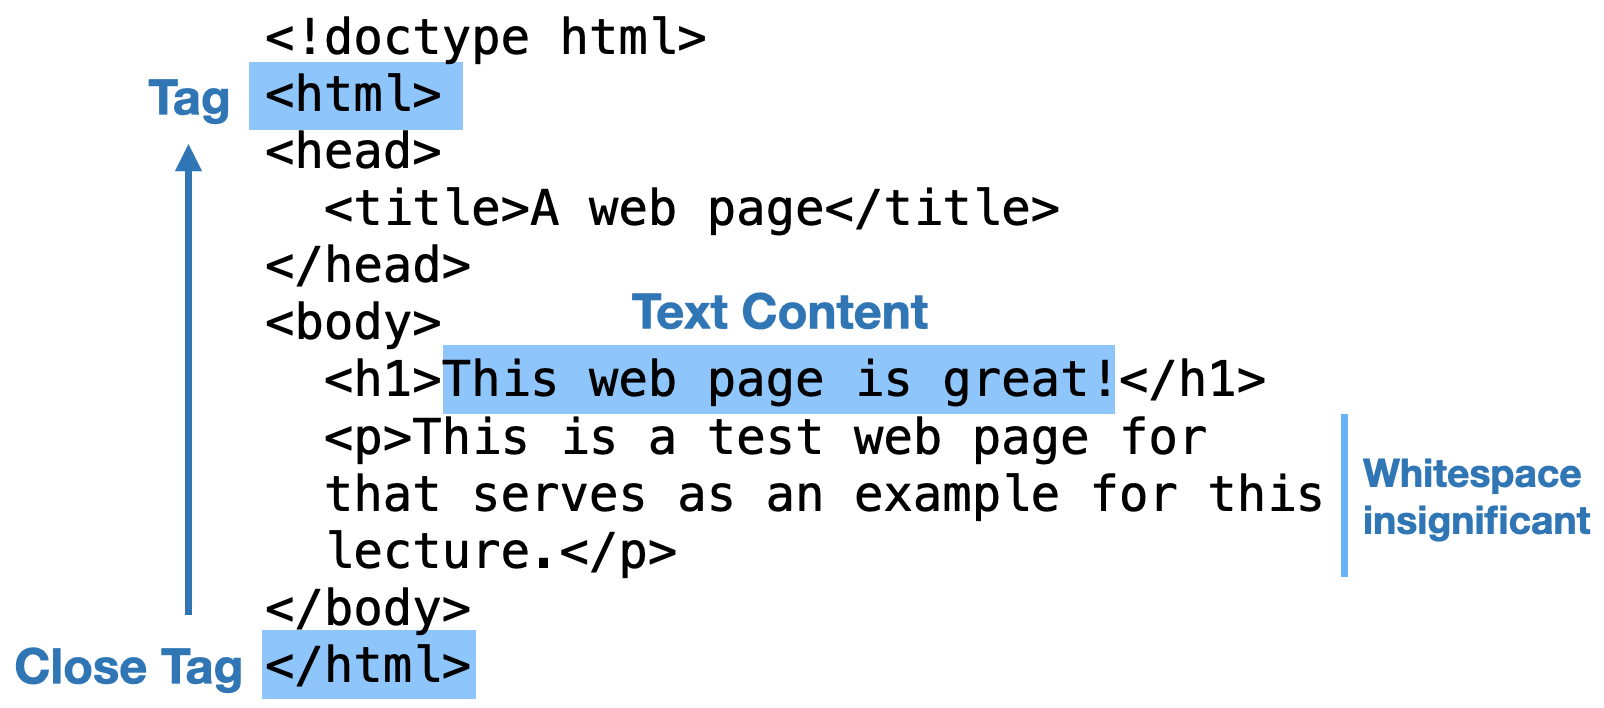
\includegraphics[width=0.8\textwidth]{im/html-syntax.png}
\caption{An HTML document, showing tags, text, and the nesting structure.}\label{fig:HTMLDoc}
\end{figure}
%\end{center}

For our browser to use a tree, tokens need to evolve into nodes. That
means adding a list of children and a parent pointer to each one. Here's
the new \texttt{Text} class, representing text at the leaf of the tree:
\begin{Shaded}
\begin{Highlighting}[]
\KeywordTok{class}\NormalTok{ Text:}
    \KeywordTok{def} \FunctionTok{\_\_init\_\_}\NormalTok{(}\VariableTok{self}\NormalTok{, text, parent):}
        \VariableTok{self}\NormalTok{.text }\OperatorTok{=}\NormalTok{ text}
        \VariableTok{self}\NormalTok{.children }\OperatorTok{=}\NormalTok{ []}
        \VariableTok{self}\NormalTok{.parent }\OperatorTok{=}\NormalTok{ parent}
\end{Highlighting}
\end{Shaded}

Since it takes two tags (the open and the close tag) to make a node,
let's rename the \texttt{Tag} class to \texttt{Element},\index{element}
and make it look like this:
\begin{Shaded}
\begin{Highlighting}[]
\KeywordTok{class}\NormalTok{ Element:}
    \KeywordTok{def} \FunctionTok{\_\_init\_\_}\NormalTok{(}\VariableTok{self}\NormalTok{, tag, parent):}
        \VariableTok{self}\NormalTok{.tag }\OperatorTok{=}\NormalTok{ tag}
        \VariableTok{self}\NormalTok{.children }\OperatorTok{=}\NormalTok{ []}
        \VariableTok{self}\NormalTok{.parent }\OperatorTok{=}\NormalTok{ parent}
\end{Highlighting}
\end{Shaded}
I added a \texttt{children} field to both \texttt{Text} and
\texttt{Element}, even though text nodes never have children, for
consistency.

Constructing a tree of nodes from source code is called parsing. A
parser builds a tree one element or text node at a time. But that means
the parser needs to store an \emph{incomplete} tree as it goes. For
example, suppose the parser has so far read this bit of HTML:
\begin{Shaded}
\begin{Highlighting}[]
\DataTypeTok{\textless{}}\KeywordTok{html}\DataTypeTok{\textgreater{}\textless{}}\KeywordTok{video}\DataTypeTok{\textgreater{}\textless{}/}\KeywordTok{video}\DataTypeTok{\textgreater{}\textless{}}\KeywordTok{section}\DataTypeTok{\textgreater{}\textless{}}\KeywordTok{h1}\DataTypeTok{\textgreater{}}\NormalTok{This is my webpage}
\end{Highlighting}
\end{Shaded}

The parser has seen five tags (and one text node). The rest of the HTML
will contain more open tags, close tags, and text, but no matter which
tokens it sees, no new nodes will be added to the
\texttt{\textless{}video\textgreater{}} tag, which has already been
closed. So that node is ``finished''. But the other nodes are
unfinished: more children can be added to the
\texttt{\textless{}html\textgreater{}},
\texttt{\textless{}section\textgreater{}}, and
\texttt{\textless{}h1\textgreater{}} nodes, depending on what HTML comes
next---see Figure~\ref{fig:UnfinishedNodes}.

\begin{figure}
\centering
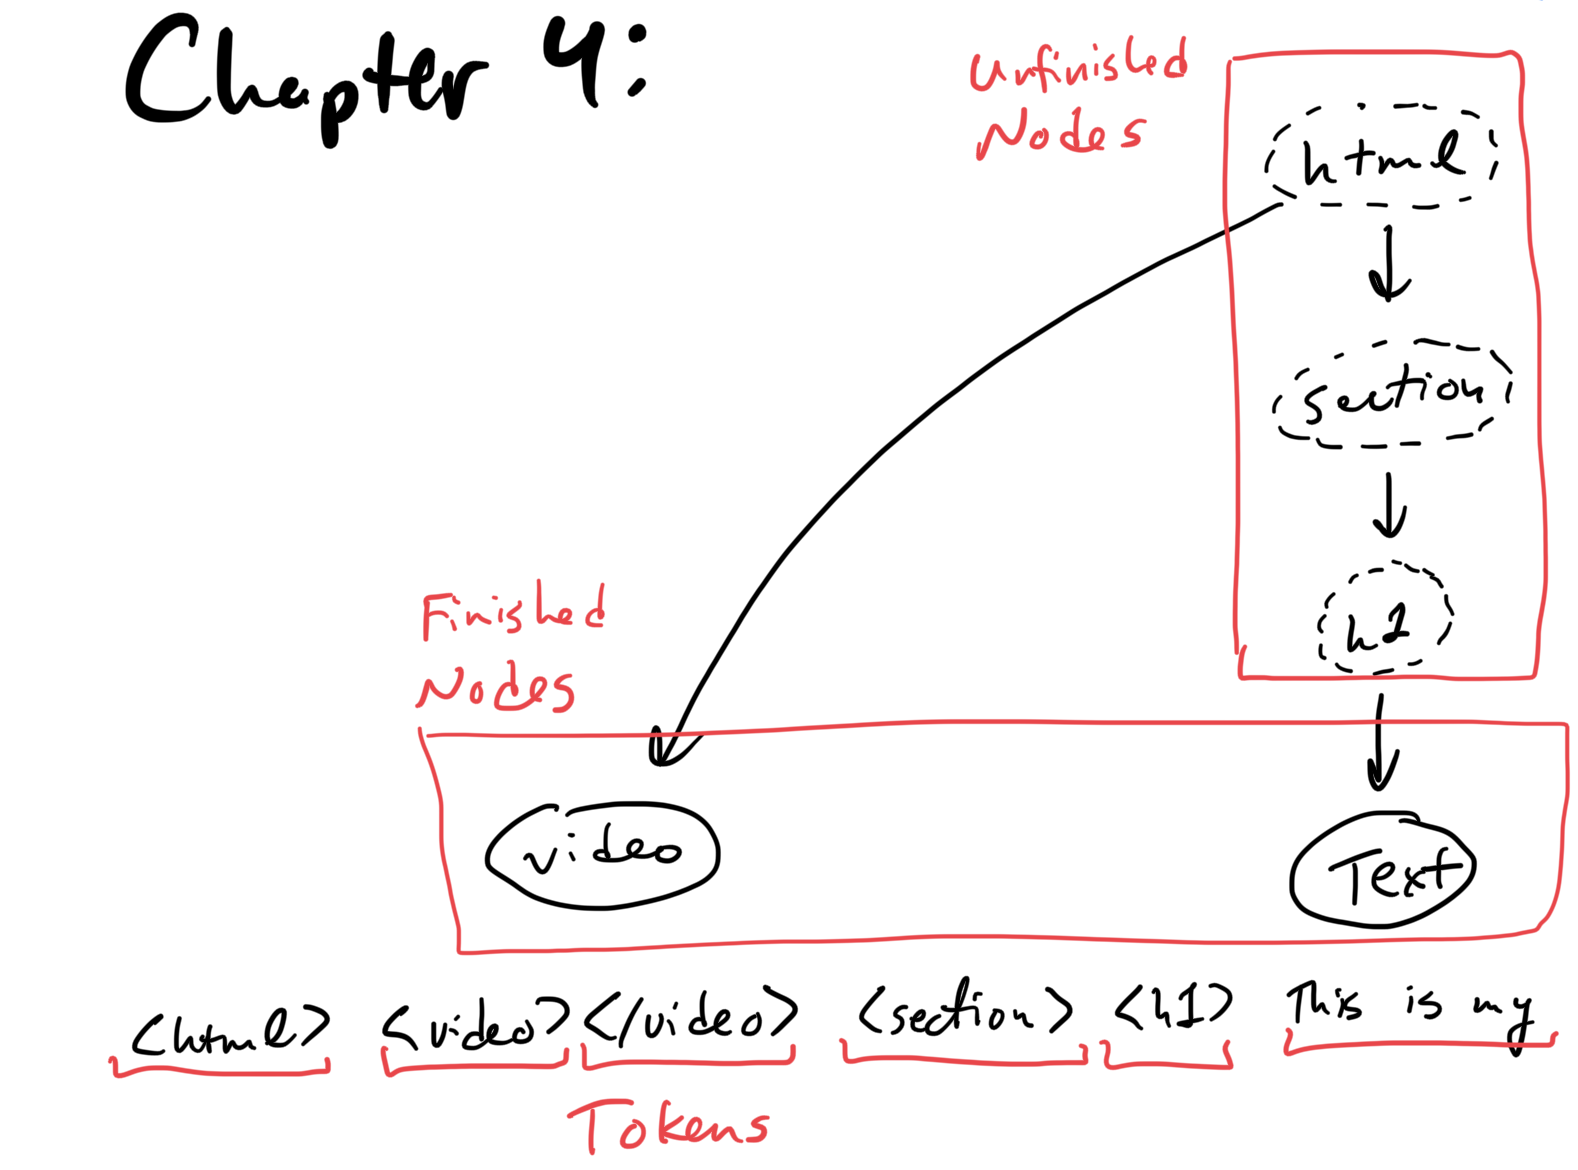
\includegraphics[width=0.8\textwidth]{im/html-lr.png}
\caption{The finished and unfinished nodes while parsing some HTML.}\label{fig:UnfinishedNodes}
\end{figure}

Since the parser reads the HTML file from beginning to end, these
unfinished tags are always in a certain part of the tree. The unfinished
tags have always been \emph{opened} but not yet closed; they are always
\emph{later in the source} than the finished nodes; and they are always
\emph{children of other unfinished tags}. To leverage these facts, let's
represent an incomplete tree by storing a list of unfinished tags,
ordered with parents before children. The first node in the list is the
root of the HTML tree; the last node in the list is the most recent
unfinished tag.\footnote{In Python, and most other languages, it's
  faster to add and remove from the end of a list, instead of the
  beginning.}

Parsing is a little more complex than \texttt{lex}, so we're going to
want to break it into several functions, organized in a new
\texttt{HTMLParser} class. That class can also store the source code
it's analyzing and the incomplete tree:
\begin{Shaded}
\begin{Highlighting}[]
\KeywordTok{class}\NormalTok{ HTMLParser:}
    \KeywordTok{def} \FunctionTok{\_\_init\_\_}\NormalTok{(}\VariableTok{self}\NormalTok{, body):}
        \VariableTok{self}\NormalTok{.body }\OperatorTok{=}\NormalTok{ body}
        \VariableTok{self}\NormalTok{.unfinished }\OperatorTok{=}\NormalTok{ []}
\end{Highlighting}
\end{Shaded}

Before the parser starts, it hasn't seen any tags at all, so the
\texttt{unfinished} list storing the tree starts empty. But as the
parser reads tokens, that list fills up. Let's start that by
aspirationally renaming the \texttt{lex} function we have now to
\texttt{parse}:
\begin{Shaded}
\begin{Highlighting}[]
\KeywordTok{class}\NormalTok{ HTMLParser:}
    \KeywordTok{def}\NormalTok{ parse(}\VariableTok{self}\NormalTok{):}
        \CommentTok{\# ...}
\end{Highlighting}
\end{Shaded}

We'll need to do a bit of surgery on \texttt{parse}. Right now
\texttt{parse} creates \texttt{Tag} and \texttt{Text} objects and
appends them to the \texttt{out} array. We need it to create
\texttt{Element} and \texttt{Text} objects and add them to the
\texttt{unfinished} tree. Since a tree is a bit more complex than a
list, I'll move the adding-to-a-tree logic to two new methods,
\texttt{add\_text} and \texttt{add\_tag}.
\begin{Shaded}
\begin{Highlighting}[]
\KeywordTok{def}\NormalTok{ parse(}\VariableTok{self}\NormalTok{):}
\NormalTok{    text }\OperatorTok{=} \StringTok{""}
\NormalTok{    in\_tag }\OperatorTok{=} \VariableTok{False}
    \ControlFlowTok{for}\NormalTok{ c }\KeywordTok{in} \VariableTok{self}\NormalTok{.body:}
        \ControlFlowTok{if}\NormalTok{ c }\OperatorTok{==} \StringTok{"\textless{}"}\NormalTok{:}
\NormalTok{            in\_tag }\OperatorTok{=} \VariableTok{True}
            \ControlFlowTok{if}\NormalTok{ text: }\VariableTok{self}\NormalTok{.add\_text(text)}
\NormalTok{            text }\OperatorTok{=} \StringTok{""}
        \ControlFlowTok{elif}\NormalTok{ c }\OperatorTok{==} \StringTok{"\textgreater{}"}\NormalTok{:}
\NormalTok{            in\_tag }\OperatorTok{=} \VariableTok{False}
            \VariableTok{self}\NormalTok{.add\_tag(text)}
\NormalTok{            text }\OperatorTok{=} \StringTok{""}
        \ControlFlowTok{else}\NormalTok{:}
\NormalTok{            text }\OperatorTok{+=}\NormalTok{ c}
    \ControlFlowTok{if} \KeywordTok{not}\NormalTok{ in\_tag }\KeywordTok{and}\NormalTok{ text:}
        \VariableTok{self}\NormalTok{.add\_text(text)}
    \ControlFlowTok{return} \VariableTok{self}\NormalTok{.finish()}
\end{Highlighting}
\end{Shaded}
The \texttt{out} variable is gone, and note that I've also moved the
return value to a new \texttt{finish} method, which converts the
incomplete tree to the final, complete tree. So: how do we add things to
the tree?

\begin{bookblock}{further}
HTML derives from a long line of document processing systems. Its
predecessor,
\href{https://en.wikipedia.org/wiki/Standard_Generalized_Markup_Language}{SGML},
traces back to
\href{https://en.wikipedia.org/wiki/TYPSET_and_RUNOFF}{RUNOFF} and is a
sibling to \href{https://troff.org}{troff}, now used for Linux manual
pages. The \href{https://www.iso.org/committee/45374.html}{committee}
that standardized SGML now works on the \texttt{.odf}, \texttt{.docx},
and \texttt{.epub} formats.

\end{bookblock}

\hypertarget{constructing-the-tree}{%
\section{Constructing the Tree}\label{constructing-the-tree}}

Let's talk about adding nodes to a tree. To add a text node we add it as
a child of the last unfinished node:
\begin{Shaded}
\begin{Highlighting}[]
\KeywordTok{class}\NormalTok{ HTMLParser:}
    \KeywordTok{def}\NormalTok{ add\_text(}\VariableTok{self}\NormalTok{, text):}
\NormalTok{        parent }\OperatorTok{=} \VariableTok{self}\NormalTok{.unfinished[}\OperatorTok{{-}}\DecValTok{1}\NormalTok{]}
\NormalTok{        node }\OperatorTok{=}\NormalTok{ Text(text, parent)}
\NormalTok{        parent.children.append(node)}
\end{Highlighting}
\end{Shaded}

On the other hand, tags are a little more complex since they might be an
open \emph{or} a close tag:
\begin{Shaded}
\begin{Highlighting}[]
\KeywordTok{class}\NormalTok{ HTMLParser:}
    \KeywordTok{def}\NormalTok{ add\_tag(}\VariableTok{self}\NormalTok{, tag):}
        \ControlFlowTok{if}\NormalTok{ tag.startswith(}\StringTok{"/"}\NormalTok{):}
            \CommentTok{\# ...}
        \ControlFlowTok{else}\NormalTok{:}
            \CommentTok{\# ...}
\end{Highlighting}
\end{Shaded}
An open tag instead adds an unfinished node to the end of the list:
\begin{Shaded}
\begin{Highlighting}[]
\KeywordTok{def}\NormalTok{ add\_tag(}\VariableTok{self}\NormalTok{, tag):}
    \CommentTok{\# ...}
    \ControlFlowTok{else}\NormalTok{:}
\NormalTok{        parent }\OperatorTok{=} \VariableTok{self}\NormalTok{.unfinished[}\OperatorTok{{-}}\DecValTok{1}\NormalTok{]}
\NormalTok{        node }\OperatorTok{=}\NormalTok{ Element(tag, parent)}
        \VariableTok{self}\NormalTok{.unfinished.append(node)}
\end{Highlighting}
\end{Shaded}
A close tag instead finishes the last unfinished node by adding it to
the previous unfinished node in the list:
\begin{Shaded}
\begin{Highlighting}[]
\KeywordTok{def}\NormalTok{ add\_tag(}\VariableTok{self}\NormalTok{, tag):}
    \ControlFlowTok{if}\NormalTok{ tag.startswith(}\StringTok{"/"}\NormalTok{):}
\NormalTok{        node }\OperatorTok{=} \VariableTok{self}\NormalTok{.unfinished.pop()}
\NormalTok{        parent }\OperatorTok{=} \VariableTok{self}\NormalTok{.unfinished[}\OperatorTok{{-}}\DecValTok{1}\NormalTok{]}
\NormalTok{        parent.children.append(node)}
    \CommentTok{\# ...}
\end{Highlighting}
\end{Shaded}

Once the parser is done, it turns our incomplete tree into a complete
tree by just finishing any unfinished nodes:
\begin{Shaded}
\begin{Highlighting}[]
\KeywordTok{class}\NormalTok{ HTMLParser:}
    \KeywordTok{def}\NormalTok{ finish(}\VariableTok{self}\NormalTok{):}
        \ControlFlowTok{while} \BuiltInTok{len}\NormalTok{(}\VariableTok{self}\NormalTok{.unfinished) }\OperatorTok{\textgreater{}} \DecValTok{1}\NormalTok{:}
\NormalTok{            node }\OperatorTok{=} \VariableTok{self}\NormalTok{.unfinished.pop()}
\NormalTok{            parent }\OperatorTok{=} \VariableTok{self}\NormalTok{.unfinished[}\OperatorTok{{-}}\DecValTok{1}\NormalTok{]}
\NormalTok{            parent.children.append(node)}
        \ControlFlowTok{return} \VariableTok{self}\NormalTok{.unfinished.pop()}
\end{Highlighting}
\end{Shaded}

This is \emph{almost} a complete parser, but it doesn't quite work at
the beginning and end of the document. The very first open tag is an
edge case without a parent:
\begin{Shaded}
\begin{Highlighting}[]
\KeywordTok{def}\NormalTok{ add\_tag(}\VariableTok{self}\NormalTok{, tag):}
    \CommentTok{\# ...}
    \ControlFlowTok{else}\NormalTok{:}
\NormalTok{        parent }\OperatorTok{=} \VariableTok{self}\NormalTok{.unfinished[}\OperatorTok{{-}}\DecValTok{1}\NormalTok{] }\ControlFlowTok{if} \VariableTok{self}\NormalTok{.unfinished }\ControlFlowTok{else} \VariableTok{None}
        \CommentTok{\# ...}
\end{Highlighting}
\end{Shaded}
The very last tag is also an edge case, because there's no unfinished
node to add it to:
\begin{Shaded}
\begin{Highlighting}[]
\KeywordTok{def}\NormalTok{ add\_tag(}\VariableTok{self}\NormalTok{, tag):}
    \ControlFlowTok{if}\NormalTok{ tag.startswith(}\StringTok{"/"}\NormalTok{):}
        \ControlFlowTok{if} \BuiltInTok{len}\NormalTok{(}\VariableTok{self}\NormalTok{.unfinished) }\OperatorTok{==} \DecValTok{1}\NormalTok{: }\ControlFlowTok{return}
        \CommentTok{\# ...}
\end{Highlighting}
\end{Shaded}
Ok, that's all done. Let's test our parser out and see how well it
works!

\begin{bookblock}{further}
The ill-considered JavaScript \texttt{document.write} method allows
JavaScript to modify the HTML source code while it's being parsed! This
is actually a
\href{https://developer.mozilla.org/en-US/docs/Web/API/Document/write}{bad
idea}. An implementation of \texttt{document.write} must have the HTML
parser stop to execute JavaScript, but that slows down requests for
images, CSS, and JavaScript used later in the page. To solve this,
modern browsers use
\href{https://developer.mozilla.org/en-US/docs/Glossary/speculative_parsing}{speculative
parsing} to start loading additional resources even before parsing is
done.
\end{bookblock}

\hypertarget{debugging-a-parser}{%
\section{Debugging a Parser}\label{debugging-a-parser}}

How do we know our parser does the right thing---that it builds the
right tree? Well the place to start is \emph{seeing} the tree it
produces. We can do that with a quick, recursive pretty-printer:
\begin{Shaded}
\begin{Highlighting}[]
\KeywordTok{def}\NormalTok{ print\_tree(node, indent}\OperatorTok{=}\DecValTok{0}\NormalTok{):}
    \BuiltInTok{print}\NormalTok{(}\StringTok{" "} \OperatorTok{*}\NormalTok{ indent, node)}
    \ControlFlowTok{for}\NormalTok{ child }\KeywordTok{in}\NormalTok{ node.children:}
\NormalTok{        print\_tree(child, indent }\OperatorTok{+} \DecValTok{2}\NormalTok{)}
\end{Highlighting}
\end{Shaded}
Here we're printing each node in the tree, and using indentation to show
the tree structure. Since we need to print each node, it's worth taking
the time to give them a nice printed form, which in Python means
defining the \texttt{\_\_repr\_\_} function:
\begin{Shaded}
\begin{Highlighting}[]
\KeywordTok{class}\NormalTok{ Text:}
    \KeywordTok{def} \FunctionTok{\_\_repr\_\_}\NormalTok{(}\VariableTok{self}\NormalTok{):}
        \ControlFlowTok{return} \BuiltInTok{repr}\NormalTok{(}\VariableTok{self}\NormalTok{.text)}

\KeywordTok{class}\NormalTok{ Element:}
    \KeywordTok{def} \FunctionTok{\_\_repr\_\_}\NormalTok{(}\VariableTok{self}\NormalTok{):}
        \ControlFlowTok{return} \StringTok{"\textless{}"} \OperatorTok{+} \VariableTok{self}\NormalTok{.tag }\OperatorTok{+} \StringTok{"\textgreater{}"}
\end{Highlighting}
\end{Shaded}
In general it's a good idea to define \texttt{\_\_repr\_\_} methods for
any data objects, and to have those \texttt{\_\_repr\_\_} methods print
all the relevant fields.

Try this out on the \href{https://browser.engineering/html.html}{web page}
corresponding to this chapter, parsing the HTML source code and then
calling \texttt{print\_tree} to visualize it:
\begin{Shaded}
\begin{Highlighting}[]
\NormalTok{body }\OperatorTok{=}\NormalTok{ URL(sys.argv[}\DecValTok{1}\NormalTok{]).request()}
\NormalTok{nodes }\OperatorTok{=}\NormalTok{ HTMLParser(body).parse()}
\NormalTok{print\_tree(nodes)}
\end{Highlighting}
\end{Shaded}
% Run it on this web page, and
You'll see something like this at the beginning:
\begin{bookblock*}{notcode}
\begin{Shaded}
\begin{Highlighting}[]
\NormalTok{ \textless{}!doctype html\textgreater{}}
\NormalTok{   \textquotesingle{}\textbackslash{}n\textquotesingle{}}
\NormalTok{   \textless{}html lang="en{-}US" xml:lang="en{-}US"\textgreater{}}
\NormalTok{     \textquotesingle{}\textbackslash{}n\textquotesingle{}}
\NormalTok{     \textless{}head\textgreater{}}
\NormalTok{       \textquotesingle{}\textbackslash{}n  \textquotesingle{}}
\NormalTok{       \textless{}meta charset="utf{-}8" /\textgreater{}}
\end{Highlighting}
\end{Shaded}
\end{bookblock*}

Immediately a couple of things stand out. Let's start at the top, with
the \texttt{\textless{}!doctype\ html\textgreater{}} tag.
This special tag, called a
\href{https://html.spec.whatwg.org/multipage/syntax.html\#the-doctype}{doctype},
is always the very first thing in an HTML document. But it's not really
an element at all, nor is it supposed to have a close tag. Our browser
won't be using the doctype for anything, so it's best to throw it
away:\footnote{Real browsers use doctypes to switch between
  standards-compliant and legacy parsing and layout modes.}
\begin{Shaded}
\begin{Highlighting}[]
\KeywordTok{def}\NormalTok{ add\_tag(}\VariableTok{self}\NormalTok{, tag):}
    \ControlFlowTok{if}\NormalTok{ tag.startswith(}\StringTok{"!"}\NormalTok{): }\ControlFlowTok{return}
    \CommentTok{\# ...}
\end{Highlighting}
\end{Shaded}
This ignores all tags that start with an exclamation mark, which not
only throws out doctype declarations but also comments, which in HTML
are written
\texttt{\textless{}!-\/-\ comment\ text\ -\/-\textgreater{}}.

Just throwing out doctypes isn't quite enough though---if you run your
parser now, it will crash. That's because after the doctype comes a
newline, which our parser treats as text and tries to insert into the
tree. Except there isn't a tree, since the parser hasn't seen any open
tags. For simplicity, let's just have our browser skip whitespace-only
text nodes to side-step the problem:\footnote{Real browsers retain
  whitespace to correctly render
  \texttt{make\textless{}span\textgreater{}\textless{}/span\textgreater{}up}
  as one word and
  \texttt{make\textless{}span\textgreater{}\ \textless{}/span\textgreater{}up}
  as two. Our browser won't. Plus, ignoring whitespace simplifies
%  \href{layout.md}{
  later chapters by avoiding a special case for
  whitespace-only text tags.}
\begin{Shaded}
\begin{Highlighting}[]
\KeywordTok{def}\NormalTok{ add\_text(}\VariableTok{self}\NormalTok{, text):}
    \ControlFlowTok{if}\NormalTok{ text.isspace(): }\ControlFlowTok{return}
    \CommentTok{\# ...}
\end{Highlighting}
\end{Shaded}

The first part of the parsed HTML tree for the
\texttt{browser.engineering} home page now looks something like this:
\begin{bookblock*}{notcode}
\begin{Shaded}
\begin{Highlighting}[]
\NormalTok{ \textless{}html lang="en{-}US" xml:lang="en{-}US"\textgreater{}}
\NormalTok{   \textless{}head\textgreater{}}
\NormalTok{     \textless{}meta charset="utf{-}8" /=""\textgreater{}}
\end{Highlighting}
\end{Shaded}
\end{bookblock*}
\noindent Our next problem: why's everything so deeply indented? Why aren't these
open elements ever closed?

\begin{bookblock}{further}
In SGML, document type declarations contained a URL which defined the
valid tags, and in older versions of HTML that was also recommended.
Browsers do use the absence of a document type declaration to
\href{https://developer.mozilla.org/en-US/docs/Web/HTML/Quirks_Mode_and_Standards_Mode}{identify}
very old, pre-SGML versions of HTML,\footnotemark\ but
don't use the URL, so \texttt{\textless{}!doctype\ html\textgreater{}}
is the best document type declaration for modern HTML.
\end{bookblock}%
\footnotetext{
There's also this crazy
  thing called ``\href{https://hsivonen.fi/doctype/}{almost standards}''
  or ``limited quirks'' mode, due to a backwards-incompatible change in
  table cell vertical layout. Yes. I don't need to make these up!
}

\hypertarget{self-closing-tags}{%
\section{Self-Closing Tags}\label{self-closing-tags}}

Elements like \texttt{\textless{}meta\textgreater{}} and
\texttt{\textless{}link\textgreater{}} are what are called self-closing:
these tags don't surround content, so you don't ever write
\texttt{\textless{}/meta\textgreater{}} or
\texttt{\textless{}/link\textgreater{}}. Our parser needs special
support for them. In HTML, there's a
\href{https://html.spec.whatwg.org/multipage/syntax.html\#void-elements}{specific
list} of these self-closing tags (the specification calls them ``void''
tags):\footnote{A lot of these tags are obscure. Browsers also support
  some additional, obsolete self-closing tags not listed here, like
  \texttt{keygen}.}
\begin{Shaded}
\begin{Highlighting}[]
\NormalTok{SELF\_CLOSING\_TAGS }\OperatorTok{=}\NormalTok{ [}
    \StringTok{"area"}\NormalTok{, }\StringTok{"base"}\NormalTok{, }\StringTok{"br"}\NormalTok{, }\StringTok{"col"}\NormalTok{, }\StringTok{"embed"}\NormalTok{, }\StringTok{"hr"}\NormalTok{, }\StringTok{"img"}\NormalTok{, }\StringTok{"input"}\NormalTok{,}
    \StringTok{"link"}\NormalTok{, }\StringTok{"meta"}\NormalTok{, }\StringTok{"param"}\NormalTok{, }\StringTok{"source"}\NormalTok{, }\StringTok{"track"}\NormalTok{, }\StringTok{"wbr"}\NormalTok{,}
\NormalTok{]}
\end{Highlighting}
\end{Shaded}

Our parser needs to auto-close tags from this list:
\begin{Shaded}
\begin{Highlighting}[]
\KeywordTok{def}\NormalTok{ add\_tag(}\VariableTok{self}\NormalTok{, tag):}
    \CommentTok{\# ...}
    \ControlFlowTok{elif}\NormalTok{ tag }\KeywordTok{in} \VariableTok{self}\NormalTok{.SELF\_CLOSING\_TAGS:}
\NormalTok{        parent }\OperatorTok{=} \VariableTok{self}\NormalTok{.unfinished[}\OperatorTok{{-}}\DecValTok{1}\NormalTok{]}
\NormalTok{        node }\OperatorTok{=}\NormalTok{ Element(tag, parent)}
\NormalTok{        parent.children.append(node)}
\end{Highlighting}
\end{Shaded}
This code looks right, but if you test it out it won't seem to help. Why
not? Because our parser is looking for a tag named \texttt{meta}, but
it's finding a tag named ``\texttt{meta\ name=...}''. The self-closing
code isn't triggered because the \texttt{\textless{}meta\textgreater{}}
tag has attributes.

HTML attributes\index{attribute} add information about an element; open
tags can have any number of attributes. Attribute values can be quoted,
unquoted, or omitted entirely. Let's focus on basic attribute support,
ignoring values that contain whitespace, which are a little complicated.

Since we're not handling whitespace in values, we can split on
whitespace to get the tag name and the attribute--value pairs:
\begin{Shaded}
\begin{Highlighting}[]
\KeywordTok{class}\NormalTok{ HTMLParser:}
    \KeywordTok{def}\NormalTok{ get\_attributes(}\VariableTok{self}\NormalTok{, text):}
\NormalTok{        parts }\OperatorTok{=}\NormalTok{ text.split()}
\NormalTok{        tag }\OperatorTok{=}\NormalTok{ parts[}\DecValTok{0}\NormalTok{].casefold()}
\NormalTok{        attributes }\OperatorTok{=}\NormalTok{ \{\}}
        \ControlFlowTok{for}\NormalTok{ attrpair }\KeywordTok{in}\NormalTok{ parts[}\DecValTok{1}\NormalTok{:]:}
            \CommentTok{\# ...}
        \ControlFlowTok{return}\NormalTok{ tag, attributes}
\end{Highlighting}
\end{Shaded}

HTML tag names are case insensitive, as by the way are attribute names,
so I case-fold them.\footnote{The \texttt{casefold} method works better
  than \texttt{lower}. Lower-casing text is the
  \href{https://www.b-list.org/weblog/2018/nov/26/case/}{wrong way} to
  do case-insensitive comparisons in languages like Cherokee. In HTML
  specifically, tag names only use the ASCII characters so lower-casing
  them would be sufficient, but I'm using Python's \texttt{casefold}
  function because it's a good habit to get into.} Then, inside the
loop, I split each attribute--value pair into a name and a value. The
easiest case is an unquoted attribute, where an equal sign separates the
two:
\begin{Shaded}
\begin{Highlighting}[]
\KeywordTok{def}\NormalTok{ get\_attributes(}\VariableTok{self}\NormalTok{, text):}
    \CommentTok{\# ...}
    \ControlFlowTok{for}\NormalTok{ attrpair }\KeywordTok{in}\NormalTok{ parts[}\DecValTok{1}\NormalTok{:]:}
        \ControlFlowTok{if} \StringTok{"="} \KeywordTok{in}\NormalTok{ attrpair:}
\NormalTok{            key, value }\OperatorTok{=}\NormalTok{ attrpair.split(}\StringTok{"="}\NormalTok{, }\DecValTok{1}\NormalTok{)}
\NormalTok{            attributes[key.casefold()] }\OperatorTok{=}\NormalTok{ value}
    \CommentTok{\# ...}
\end{Highlighting}
\end{Shaded}

The value can also be omitted, like in
\texttt{\textless{}input\ disabled\textgreater{}}, in which case the
attribute value defaults to the empty string:
\begin{Shaded}
\begin{Highlighting}[]
\ControlFlowTok{for}\NormalTok{ attrpair }\KeywordTok{in}\NormalTok{ parts[}\DecValTok{1}\NormalTok{:]:}
    \CommentTok{\# ...}
    \ControlFlowTok{else}\NormalTok{:}
\NormalTok{        attributes[attrpair.casefold()] }\OperatorTok{=} \StringTok{""}
\end{Highlighting}
\end{Shaded}

Finally, the value can be quoted, in which case the quotes have to be
stripped out:\footnote{Quoted attributes allow whitespace between the
  quotes. That requires something like a finite state machine instead of
  just splitting on whitespace.}
\begin{Shaded}
\begin{Highlighting}[]
\ControlFlowTok{if} \StringTok{"="} \KeywordTok{in}\NormalTok{ attrpair:}
    \CommentTok{\# ...}
    \ControlFlowTok{if} \BuiltInTok{len}\NormalTok{(value) }\OperatorTok{\textgreater{}} \DecValTok{2} \KeywordTok{and}\NormalTok{ value[}\DecValTok{0}\NormalTok{] }\KeywordTok{in}\NormalTok{ [}\StringTok{"\textquotesingle{}"}\NormalTok{, }\StringTok{"}\CharTok{\textbackslash{}"}\StringTok{"}\NormalTok{]:}
\NormalTok{        value }\OperatorTok{=}\NormalTok{ value[}\DecValTok{1}\NormalTok{:}\OperatorTok{{-}}\DecValTok{1}\NormalTok{]}
    \CommentTok{\# ...}
\end{Highlighting}
\end{Shaded}

We'll store these attributes inside \texttt{Element}s:
\begin{Shaded}
\begin{Highlighting}[]
\KeywordTok{class}\NormalTok{ Element:}
    \KeywordTok{def} \FunctionTok{\_\_init\_\_}\NormalTok{(}\VariableTok{self}\NormalTok{, tag, attributes, parent):}
        \VariableTok{self}\NormalTok{.tag }\OperatorTok{=}\NormalTok{ tag}
        \VariableTok{self}\NormalTok{.attributes }\OperatorTok{=}\NormalTok{ attributes}
        \CommentTok{\# ...}
\end{Highlighting}
\end{Shaded}
That means we'll need to call \texttt{get\_attributes} at the top of
\texttt{add\_tag}, to get the \texttt{attributes} we need to construct
an \texttt{Element}.
\begin{Shaded}
\begin{Highlighting}[]
\KeywordTok{def}\NormalTok{ add\_tag(}\VariableTok{self}\NormalTok{, tag):}
\NormalTok{    tag, attributes }\OperatorTok{=} \VariableTok{self}\NormalTok{.get\_attributes(tag)}
\end{Highlighting}
\end{Shaded}

Remember to use \texttt{tag} and \texttt{attribute} instead of
\texttt{text} in \texttt{add\_tag}, and try your parser again:
\begin{bookblock*}{notcode}
\begin{Shaded}
\begin{Highlighting}[]
\NormalTok{\textless{}html\textgreater{}}
\NormalTok{   \textless{}head\textgreater{}}
\NormalTok{     \textless{}meta\textgreater{}}
\NormalTok{     \textless{}link\textgreater{}}
\NormalTok{     \textless{}link\textgreater{}}
\NormalTok{     \textless{}link\textgreater{}}
\NormalTok{     \textless{}link\textgreater{}}
\NormalTok{     \textless{}link\textgreater{}}
\NormalTok{     \textless{}meta\textgreater{}}
\end{Highlighting}
\end{Shaded}
\end{bookblock*}
\noindent It's close! Yes, if you print the attributes, you'll see that attributes
with whitespace (like \texttt{author} on the fifth \texttt{meta} tag)
are mis-parsed as multiple attributes, and the final slash on the
self-closing tags is incorrectly treated as an extra attribute. A better
parser would fix these issues. But let's instead leave our parser as
is---these issues aren't going to be a problem for the browser we're
building---and move on to integrating it with our browser.

\begin{bookblock}{further}
Putting a slash at the end of self-closing tags, like
\texttt{\textless{}br/\textgreater{}}, became fashionable when
\href{https://www.w3.org/TR/xhtml1/}{XHTML} looked like it might replace
HTML, and old-timers like me never broke the habit. But unlike in
\href{https://www.w3.org/TR/xml/\#sec-starttags}{XML}, in HTML
self-closing tags are identified by name, not by some special syntax, so
the slash is optional.
\end{bookblock}

\hypertarget{using-the-node-tree}{%
\section{Using the Node Tree}\label{using-the-node-tree}}

Right now, the \texttt{Layout} class works token by token; we now want
it to go node by node instead. So let's separate the old \texttt{token}
method into two parts: all the cases for open tags will go into a new
\texttt{open\_tag} method and all the cases for close tags will go into
a new \texttt{close\_tag} method:\footnote{The case for text tokens is
  no longer needed because our browser can just call the existing
  \texttt{text} method directly.}
\begin{Shaded}
\begin{Highlighting}[]
\KeywordTok{class}\NormalTok{ Layout:}
    \KeywordTok{def}\NormalTok{ open\_tag(}\VariableTok{self}\NormalTok{, tag):}
        \ControlFlowTok{if}\NormalTok{ tag }\OperatorTok{==} \StringTok{"i"}\NormalTok{:}
            \VariableTok{self}\NormalTok{.style }\OperatorTok{=} \StringTok{"italic"}
        \CommentTok{\# ...}

    \KeywordTok{def}\NormalTok{ close\_tag(}\VariableTok{self}\NormalTok{, tag):}
        \ControlFlowTok{if}\NormalTok{ tag }\OperatorTok{==} \StringTok{"i"}\NormalTok{:}
            \VariableTok{self}\NormalTok{.style }\OperatorTok{=} \StringTok{"roman"}
        \CommentTok{\# ...}
\end{Highlighting}
\end{Shaded}

Now we need the \texttt{Layout} object to walk the node tree, calling
\texttt{open\_tag}, \texttt{close\_tag}, and \texttt{text} in the right
order:
\begin{Shaded}
\begin{Highlighting}[]
\KeywordTok{def}\NormalTok{ recurse(}\VariableTok{self}\NormalTok{, tree):}
    \ControlFlowTok{if} \BuiltInTok{isinstance}\NormalTok{(tree, Text):}
        \ControlFlowTok{for}\NormalTok{ word }\KeywordTok{in}\NormalTok{ tree.text.split():}
            \VariableTok{self}\NormalTok{.word(word)}
    \ControlFlowTok{else}\NormalTok{:}
        \VariableTok{self}\NormalTok{.open\_tag(tree.tag)}
        \ControlFlowTok{for}\NormalTok{ child }\KeywordTok{in}\NormalTok{ tree.children:}
            \VariableTok{self}\NormalTok{.recurse(child)}
        \VariableTok{self}\NormalTok{.close\_tag(tree.tag)}
\end{Highlighting}
\end{Shaded}

The \texttt{Layout} constructor can now call \texttt{recurse} instead of
looping through the list of tokens. We'll also need the browser to
construct the node tree, like this:
\begin{Shaded}
\begin{Highlighting}[]
\KeywordTok{class}\NormalTok{ Browser:}
    \KeywordTok{def}\NormalTok{ load(}\VariableTok{self}\NormalTok{, url):}
\NormalTok{        body }\OperatorTok{=}\NormalTok{ url.request()}
        \VariableTok{self}\NormalTok{.nodes }\OperatorTok{=}\NormalTok{ HTMLParser(body).parse()}
        \VariableTok{self}\NormalTok{.display\_list }\OperatorTok{=}\NormalTok{ Layout(}\VariableTok{self}\NormalTok{.nodes).display\_list}
        \VariableTok{self}\NormalTok{.draw()}
\end{Highlighting}
\end{Shaded}

Run it---the browser should now use the parsed HTML tree.

\begin{bookblock}{further}
The \texttt{doctype} syntax is a form of versioning---declaring which
version of HTML the web page is using. But in fact, the \texttt{html}
value for \texttt{doctype} signals not just a particular version of
HTML, but more generally the
\href{https://html.spec.whatwg.org/}{\emph{HTML living
standard}}.\footnotemark\ It's called a ``living
standard'' because it changes all the time as features are added. The
mechanism for these changes is simply browsers shipping new features,
not any change to the ``version'' of HTML. In general, the web is an
\emph{unversioned platform}---new features are often added as
enhancements, but only so long as they don't break existing
ones.\footnotemark
\end{bookblock}
\footnotetext[\numexpr(\value{footnote}-1)]{
It is not expected that any new \texttt{doctype}
  version for HTML will ever be added again.
}
\footnotetext{
Features can be removed, but only if they stop being used
  by the vast majority of sites. This makes it very hard to remove web
  features compared with other platforms.
}

\hypertarget{handling-author-errors}{%
\section{Handling Author Errors}\label{handling-author-errors}}

The parser now handles HTML pages correctly---at least when the HTML is
written by the sorts of goody-two-shoes programmers who remember the
\texttt{\textless{}head\textgreater{}} tag, close every open tag, and
make their bed in the morning. Mere mortals lack such discipline and so
browsers also have to handle broken, confusing, \texttt{head}less HTML. In fact,
modern HTML parsers are capable of transforming \emph{any} string of
characters into an HTML tree, no matter how confusing the
markup.\footnote{Yes, it's crazy, and for a few years in the early 2000s
  the W3C tried to \href{https://www.w3.org/TR/xhtml1/}{do away with
  it}. They failed.}

The full algorithm is, as you might expect, complicated beyond belief,
with dozens of ever-more-special cases forming a taxonomy of human
error, but one of its nicer features is \emph{implicit} tags. Normally,
an HTML document starts with a familiar boilerplate:
\begin{bookblock*}{notcode}
\begin{Shaded}
\begin{Highlighting}[]
\DataTypeTok{\textless{}!doctype }\NormalTok{html}\DataTypeTok{\textgreater{}}
\KeywordTok{\textless{}html\textgreater{}}
  \KeywordTok{\textless{}head\textgreater{}}
  \KeywordTok{\textless{}/head\textgreater{}}
  \KeywordTok{\textless{}body\textgreater{}}
  \KeywordTok{\textless{}/body\textgreater{}}
\KeywordTok{\textless{}/html\textgreater{}}
\end{Highlighting}
\end{Shaded}
\end{bookblock*}
\noindent In reality, \emph{all six} of these tags, except the doctype, are
optional: browsers insert them automatically when the web page omits
them. Let's insert implicit tags in our browser via a new
\texttt{implicit\_tags} function. We'll want to call it in both
\texttt{add\_text} and \texttt{add\_tag}:
\begin{Shaded}
\begin{Highlighting}[]
\KeywordTok{class}\NormalTok{ HTMLParser:}
    \KeywordTok{def}\NormalTok{ add\_text(}\VariableTok{self}\NormalTok{, text):}
        \ControlFlowTok{if}\NormalTok{ text.isspace(): }\ControlFlowTok{return}
        \VariableTok{self}\NormalTok{.implicit\_tags(}\VariableTok{None}\NormalTok{)}
        \CommentTok{\# ...}

    \KeywordTok{def}\NormalTok{ add\_tag(}\VariableTok{self}\NormalTok{, tag):}
\NormalTok{        tag, attributes }\OperatorTok{=} \VariableTok{self}\NormalTok{.get\_attributes(tag)}
        \ControlFlowTok{if}\NormalTok{ tag.startswith(}\StringTok{"!"}\NormalTok{): }\ControlFlowTok{return}
        \VariableTok{self}\NormalTok{.implicit\_tags(tag)}
        \CommentTok{\# ...}
\end{Highlighting}
\end{Shaded}
Note that \texttt{implicit\_tags} isn't called for the ignored
whitespace and doctypes. Let's also call it in \texttt{finish}, to make
sure that an \texttt{\textless{}html\textgreater{}} and
\texttt{\textless{}body\textgreater{}} tag are created even for empty
strings:
\begin{Shaded}
\begin{Highlighting}[]
\KeywordTok{class}\NormalTok{ HTMLParser:}
    \KeywordTok{def}\NormalTok{ finish(}\VariableTok{self}\NormalTok{):}
        \ControlFlowTok{if} \KeywordTok{not} \VariableTok{self}\NormalTok{.unfinished:}
            \VariableTok{self}\NormalTok{.implicit\_tags(}\VariableTok{None}\NormalTok{)}
        \CommentTok{\# ...}
\end{Highlighting}
\end{Shaded}

The argument to \texttt{implicit\_tags} is the tag name (or
\texttt{None} for text nodes), which we'll compare to the list of
unfinished tags to determine what's been omitted:
\begin{Shaded}
\begin{Highlighting}[]
\KeywordTok{class}\NormalTok{ HTMLParser:}
    \KeywordTok{def}\NormalTok{ implicit\_tags(}\VariableTok{self}\NormalTok{, tag):}
        \ControlFlowTok{while} \VariableTok{True}\NormalTok{:}
\NormalTok{            open\_tags }\OperatorTok{=}\NormalTok{ [node.tag }\ControlFlowTok{for}\NormalTok{ node }\KeywordTok{in} \VariableTok{self}\NormalTok{.unfinished]}
            \CommentTok{\# ...}
\end{Highlighting}
\end{Shaded}
\texttt{implicit\_tags} has a loop because more than one tag could have
been omitted in a row; every iteration around the loop will add just
one. To determine which implicit tag to add, if any, requires examining
the open tags and the tag being inserted.

Let's start with the easiest case, the implicit
\texttt{\textless{}html\textgreater{}} tag. An implicit
\texttt{\textless{}html\textgreater{}} tag is necessary if the first tag
in the document is something other than
\texttt{\textless{}html\textgreater{}}:
\begin{Shaded}
\begin{Highlighting}[]
\ControlFlowTok{while} \VariableTok{True}\NormalTok{:}
    \CommentTok{\# ...}
    \ControlFlowTok{if}\NormalTok{ open\_tags }\OperatorTok{==}\NormalTok{ [] }\KeywordTok{and}\NormalTok{ tag }\OperatorTok{!=} \StringTok{"html"}\NormalTok{:}
        \VariableTok{self}\NormalTok{.add\_tag(}\StringTok{"html"}\NormalTok{)}
\end{Highlighting}
\end{Shaded}

Both \texttt{\textless{}head\textgreater{}} and
\texttt{\textless{}body\textgreater{}} can also be omitted, but to
figure out which it is we need to look at which tag is being added:
\begin{Shaded}
\begin{Highlighting}[]
\ControlFlowTok{while} \VariableTok{True}\NormalTok{:}
    \CommentTok{\# ...}
    \ControlFlowTok{elif}\NormalTok{ open\_tags }\OperatorTok{==}\NormalTok{ [}\StringTok{"html"}\NormalTok{] }\OperatorTok{\textbackslash{}}
         \KeywordTok{and}\NormalTok{ tag }\KeywordTok{not} \KeywordTok{in}\NormalTok{ [}\StringTok{"head"}\NormalTok{, }\StringTok{"body"}\NormalTok{, }\StringTok{"/html"}\NormalTok{]:}
        \ControlFlowTok{if}\NormalTok{ tag }\KeywordTok{in} \VariableTok{self}\NormalTok{.HEAD\_TAGS:}
            \VariableTok{self}\NormalTok{.add\_tag(}\StringTok{"head"}\NormalTok{)}
        \ControlFlowTok{else}\NormalTok{:}
            \VariableTok{self}\NormalTok{.add\_tag(}\StringTok{"body"}\NormalTok{)}
\end{Highlighting}
\end{Shaded}
Here, \texttt{HEAD\_TAGS} lists the tags that you're supposed to put
into the \texttt{\textless{}head\textgreater{}} element:\footnote{The
  \texttt{\textless{}script\textgreater{}}\index{script} tag can go in
  either the head or the body section, but it goes into the head by
  default.}
\begin{Shaded}
\begin{Highlighting}[]
\KeywordTok{class}\NormalTok{ HTMLParser:}
\NormalTok{    HEAD\_TAGS }\OperatorTok{=}\NormalTok{ [}
        \StringTok{"base"}\NormalTok{, }\StringTok{"basefont"}\NormalTok{, }\StringTok{"bgsound"}\NormalTok{, }\StringTok{"noscript"}\NormalTok{,}
        \StringTok{"link"}\NormalTok{, }\StringTok{"meta"}\NormalTok{, }\StringTok{"title"}\NormalTok{, }\StringTok{"style"}\NormalTok{, }\StringTok{"script"}\NormalTok{,}
\NormalTok{    ]}
\end{Highlighting}
\end{Shaded}

Note that if both the \texttt{\textless{}html\textgreater{}} and
\texttt{\textless{}head\textgreater{}} tags are omitted,
\texttt{implicit\_tags} is going to insert both of them by going around
the loop twice. In the first iteration \texttt{open\_tags} is
\texttt{{[}{]}}, so the code adds an
\texttt{\textless{}html\textgreater{}} tag; then, in the second
iteration, \texttt{open\_tags} is \texttt{{[}"html"{]}} so it adds a
\texttt{\textless{}head\textgreater{}} tag.\footnote{These
  \texttt{add\_tag} methods themselves call \texttt{implicit\_tags},
  which means you can get into an infinite loop if you forget a case.
  I've been careful to make sure that every tag added by
  \texttt{implicit\_tags} doesn't itself trigger more implicit tags.}

Finally, the \texttt{\textless{}/head\textgreater{}} tag can also be
implicit, if the parser is inside the
\texttt{\textless{}head\textgreater{}} and sees an element that's
supposed to go in the \texttt{\textless{}body\textgreater{}}:
\begin{Shaded}
\begin{Highlighting}[]
\ControlFlowTok{while} \VariableTok{True}\NormalTok{:}
    \CommentTok{\# ...}
    \ControlFlowTok{elif}\NormalTok{ open\_tags }\OperatorTok{==}\NormalTok{ [}\StringTok{"html"}\NormalTok{, }\StringTok{"head"}\NormalTok{] }\KeywordTok{and} \OperatorTok{\textbackslash{}}
\NormalTok{         tag }\KeywordTok{not} \KeywordTok{in}\NormalTok{ [}\StringTok{"/head"}\NormalTok{] }\OperatorTok{+} \VariableTok{self}\NormalTok{.HEAD\_TAGS:}
        \VariableTok{self}\NormalTok{.add\_tag(}\StringTok{"/head"}\NormalTok{)}
\end{Highlighting}
\end{Shaded}

Technically, the \texttt{\textless{}/body\textgreater{}} and
\texttt{\textless{}/html\textgreater{}} tags can also be implicit. But
since our \texttt{finish} function already closes any unfinished tags,
that doesn't need any extra code. So all that's left for
\texttt{implicit\_tags} % tags
is to exit out of the loop:
\begin{Shaded}
\begin{Highlighting}[]
\ControlFlowTok{while} \VariableTok{True}\NormalTok{:}
    \CommentTok{\# ...}
    \ControlFlowTok{else}\NormalTok{:}
        \ControlFlowTok{break}
\end{Highlighting}
\end{Shaded}

Of course, there are more rules for handling malformed HTML: formatting
tags, nested paragraphs, embedded Scalable Vector Graphics (SVG) and MathML, and all sorts of other
complexity. Each has complicated rules abounding with edge cases. But
let's end our discussion of handling author errors here.

The rules for malformed HTML may seem arbitrary, and they are: they
evolved over years of trying to guess what people ``meant'' when they
wrote that HTML, and are now codified in the
\href{https://html.spec.whatwg.org/multipage/parsing.html}{HTML parsing
standard}. Of course, sometimes these rules ``guess'' wrong---but as so
often happens on the web, it's often more important that every browser
does the \emph{same} thing, rather than each trying to guess what the
\emph{right} thing is.

And now for the payoff! % Here is
Figure~\ref{fig:BrowserEngineering} shows a screenshot of our very own
\href{https://browser.engineering/index.html}{website},
loaded in our own browser.\footnote{To be fair, it actually looks about
  the same with the Chapter~\ref{ch:FormattingText} browser.}

%\begin{center}
\begin{figure}
  \centering
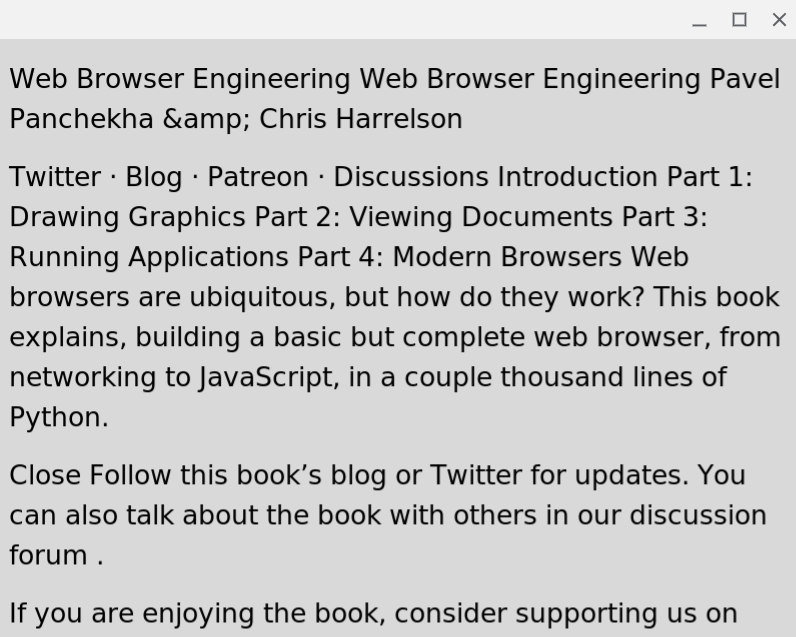
\includegraphics[width=0.8\textwidth]{examples/example4-browserengineering-screenshot.png}
\caption{\url{https://browser.engineering/index.html}
  viewed in this chapter's version of the browser.}\label{fig:BrowserEngineering}
\end{figure}
%\end{center}

\begin{bookblock}{further}
Thanks to implicit tags, you can mostly skip the
\texttt{\textless{}html\textgreater{}},
\texttt{\textless{}body\textgreater{}}, and
\texttt{\textless{}head\textgreater{}} elements, and they'll be
implicitly added back for you. In fact, the HTML parser's
\href{https://html.spec.whatwg.org/multipage/parsing.html\#parsing-main-afterbody}{many
states} guarantee something stricter than that: every HTML document has
exactly one \texttt{\textless{}head\textgreater{}} and one
\texttt{\textless{}body\textgreater{}}, in the expected
order.\footnotemark
\end{bookblock}
\footnotetext{
At least, per document. An HTML file that uses frames or
  templates can have more than one
  \texttt{\textless{}head\textgreater{}} and
  \texttt{\textless{}body\textgreater{}}, but they correspond to
  different documents.
}

\hypertarget{summary}{%
\section{Summary}\label{DocumentTree-summary}}

This chapter taught our browser that HTML is a tree, not just a flat
list of tokens. We added:
\begin{itemize}
\tightlist
\item
  a parser to transform HTML tokens to a tree;
\item
  code to recognize and handle attributes on elements;
\item
  automatic fixes for some malformed HTML documents;
\item
  a recursive layout algorithm to lay out an HTML tree.
\end{itemize}
The tree structure of HTML is essential to display visually complex web
pages, as we will see in the % \href{layout.md}{
next chapter.

\hypertarget{outline}{%
\section{Outline}\label{DocumentTree-outline}}

The complete set of functions, classes, and methods in our browser
should look something like this:
\begin{Shaded}
\begin{Highlighting}[]
\KeywordTok{class}\NormalTok{ URL:}
    \KeywordTok{def} \FunctionTok{\_\_init\_\_}\NormalTok{(url)}
    \KeywordTok{def}\NormalTok{ request()}
\NormalTok{WIDTH}
\NormalTok{HEIGHT}
\NormalTok{HSTEP}
\NormalTok{VSTEP}
\NormalTok{SCROLL\_STEP}
\NormalTok{FONTS}
\KeywordTok{def}\NormalTok{ get\_font(size, weight, slant)}
\KeywordTok{class}\NormalTok{ Layout:}
    \KeywordTok{def} \FunctionTok{\_\_init\_\_}\NormalTok{(tree)}
    \KeywordTok{def}\NormalTok{ token(tok)}
    \KeywordTok{def}\NormalTok{ word(word)}
    \KeywordTok{def}\NormalTok{ flush()}
    \KeywordTok{def}\NormalTok{ recurse(tree)}
    \KeywordTok{def}\NormalTok{ open\_tag(tag)}
    \KeywordTok{def}\NormalTok{ close\_tag(tag)}
\KeywordTok{class}\NormalTok{ Browser:}
    \KeywordTok{def} \FunctionTok{\_\_init\_\_}\NormalTok{()}
    \KeywordTok{def}\NormalTok{ load(url)}
    \KeywordTok{def}\NormalTok{ draw()}
    \KeywordTok{def}\NormalTok{ scrolldown(e)}
\KeywordTok{class}\NormalTok{ Text:}
    \KeywordTok{def} \FunctionTok{\_\_init\_\_}\NormalTok{(text, parent)}
    \KeywordTok{def} \FunctionTok{\_\_repr\_\_}\NormalTok{()}
\KeywordTok{class}\NormalTok{ Element:}
    \KeywordTok{def} \FunctionTok{\_\_init\_\_}\NormalTok{(tag, attributes, parent)}
    \KeywordTok{def} \FunctionTok{\_\_repr\_\_}\NormalTok{()}
\KeywordTok{def}\NormalTok{ print\_tree(node, indent)}
\KeywordTok{class}\NormalTok{ HTMLParser:}
    \KeywordTok{def} \FunctionTok{\_\_init\_\_}\NormalTok{(body)}
    \KeywordTok{def}\NormalTok{ parse()}
    \KeywordTok{def}\NormalTok{ get\_attributes(text)}
    \KeywordTok{def}\NormalTok{ add\_text(text)}
\NormalTok{    SELF\_CLOSING\_TAGS}
    \KeywordTok{def}\NormalTok{ add\_tag(tag)}
\NormalTok{    HEAD\_TAGS}
    \KeywordTok{def}\NormalTok{ implicit\_tags(tag)}
    \KeywordTok{def}\NormalTok{ finish()}
\end{Highlighting}
\end{Shaded}

\hypertarget{exercises}{%
\section{Exercises}\label{DocumentTree-exercises}}
\begin{enumerate}[label=\thechapter-\arabic*]
\item\emph{Comments.} Update the HTML lexer to support comments. Comments in
HTML begin with \texttt{\textless{}!-\/-} and end with
\texttt{-\/-\textgreater{}}. However, comments aren't the same as tags:
they can contain any text, including left and right angle brackets. The
lexer should skip comments, not generating any token at all. Check: is
\texttt{\textless{}!-\/-\textgreater{}} a comment, or does it just start
one?

\item\emph{Paragraphs.} It's not clear what it would mean for one paragraph
to contain another. Change the parser so that a document like
\texttt{\textless{}p\textgreater{}hello\textless{}p\textgreater{}world\textless{}/p\textgreater{}}
results in two sibling paragraphs instead of one paragraph inside
another; real browsers do this too. Do the same for
\texttt{\textless{}li\textgreater{}} elements, but make sure nested
lists are still possible.

\item\emph{Scripts.} JavaScript code embedded in a
\texttt{\textless{}script\textgreater{}} tag uses the left angle bracket
to mean ``less than''. Modify your lexer so that the contents of
\texttt{\textless{}script\textgreater{}} tags are treated specially: no
tags are allowed inside \texttt{\textless{}script\textgreater{}}, except
the \texttt{\textless{}/script\textgreater{}} close tag.\footnote{Technically
  it's just \texttt{\textless{}/script} followed by a
  \href{https://html.spec.whatwg.org/multipage/parsing.html\#script-data-end-tag-name-state}{space,
  tab, \texttt{\textbackslash{}v}, \texttt{\textbackslash{}r}, slash, or
  greater than sign}. If you need to talk about
  \texttt{\textless{}/script\textgreater{}} tags inside JavaScript code,
  you have to split it into multiple strings.}

\item\emph{Quoted attributes.} Quoted attributes can contain spaces and right
angle brackets. Fix the lexer so that this is supported properly. Hint:
the current lexer is a finite state machine, with two states (determined
by \texttt{in\_tag}). You'll need more states.

\item\emph{Syntax highlighting.} Implement the \texttt{view-source} protocol
as in % \href{http.md\#exercises}{Chapter 1}
Exercise~\ref{ex:view-source}, but make it syntax-highlight
the source code of HTML pages. Keep source code for HTML tags in a
normal font, but make text contents bold. If you've implemented it, wrap
text in \texttt{\textless{}pre\textgreater{}} tags as well to preserve
line breaks. Hint: subclass the HTML parser and use it to implement your
syntax highlighter.

\item\emph{Mis-nested formatting tags.} Extend your HTML parser to support
markup like
\texttt{\textless{}b\textgreater{}Bold\ \textless{}i\textgreater{}both\textless{}/b\textgreater{}\ italic\textless{}/i\textgreater{}}.
This requires keeping track of the set of open text formatting elements
and inserting implicit open and close tags when text formatting elements
are closed in the wrong order. The bold/italic example, for example,
should insert an implicit \texttt{\textless{}/i\textgreater{}} before
the \texttt{\textless{}/b\textgreater{}} and an implicit
\texttt{\textless{}i\textgreater{}} after it.
\end{enumerate}

\ifprintedoutput
\theendnotes
\setcounter{endnote}{0}
\fi

\chapter{Laying Out Pages}\label{ch:LayingOutPages}
So far, layout has been a linear process that handles open tags and
close tags independently. But web pages are trees, and look like them:
borders and backgrounds visually nest inside one another. To support
that, this chapter switches to \emph{tree-based layout},\index{layout}
where the tree of elements is transformed into a tree of \emph{layout
objects} before drawing. In the process, we'll make web pages more
colorful with backgrounds.

\hypertarget{the-layout-tree}{%
\section{The Layout Tree}\label{the-layout-tree}}

Right now, our browser lays out an element's open and close tags
separately. Both tags modify global state, like the \texttt{cursor\_x}
and \texttt{cursor\_y} variables, but they aren't otherwise connected,
and information about the element as a whole, like its width and height,
is never computed. That makes it pretty hard to draw a background behind
an element, let alone more complicated visual effects. So web browsers
structure layout differently.

In a browser, layout is about producing a \emph{layout
tree},\index{layout!tree} whose nodes are \emph{layout objects}, each
associated with an HTML element\footnote{Elements like
  \texttt{\textless{}script\textgreater{}} don't generate layout
  objects, and some elements generate multiple layout objects
  (\texttt{\textless{}li\textgreater{}} elements have an extra one
  for the bullet point!), but mostly it's one layout object each.} and
each with a size and a position. The browser walks the HTML tree to
produce the layout tree, then computes the size and position for each
layout object, and finally draws each layout object to the screen.

Let's start by looking at how the existing \texttt{Layout} class is used:
\begin{Shaded}
\begin{Highlighting}[]
\KeywordTok{class}\NormalTok{ Browser:}
    \KeywordTok{def}\NormalTok{ load(}\VariableTok{self}\NormalTok{, url):}
        \CommentTok{\# ...}
        \VariableTok{self}\NormalTok{.display\_list }\OperatorTok{=}\NormalTok{ Layout(}\VariableTok{self}\NormalTok{.nodes).display\_list}
        \CommentTok{\#...}
\end{Highlighting}
\end{Shaded}
Here, a \texttt{Layout} object is created briefly and then thrown away.
Let's instead make it the beginning of our layout tree by storing it in
a \texttt{Browser} field:
\begin{Shaded}
\begin{Highlighting}[]
\KeywordTok{class}\NormalTok{ Browser:}
    \KeywordTok{def}\NormalTok{ load(}\VariableTok{self}\NormalTok{, url):}
        \CommentTok{\# ...}
        \VariableTok{self}\NormalTok{.document }\OperatorTok{=}\NormalTok{ Layout(}\VariableTok{self}\NormalTok{.nodes)}
        \VariableTok{self}\NormalTok{.document.layout()}
        \CommentTok{\#...}
\end{Highlighting}
\end{Shaded}
Note that I've renamed the \texttt{Layout} constructor to a
\texttt{layout} method, so that constructing a layout object and
actually laying it out can be different steps. The constructor now just
stores the node it was passed:
\begin{Shaded}
\begin{Highlighting}[]
\KeywordTok{class}\NormalTok{ Layout:}
    \KeywordTok{def} \FunctionTok{\_\_init\_\_}\NormalTok{(}\VariableTok{self}\NormalTok{, node):}
        \VariableTok{self}\NormalTok{.node }\OperatorTok{=}\NormalTok{ node}
\end{Highlighting}
\end{Shaded}

So far, we still don't have a tree---we just have a single
\texttt{Layout} object. To make it into a tree, we'll need to add child and
parent pointers. I'm also going to add a pointer to the previous
sibling, because that'll be useful for computing sizes and positions
later:
\begin{Shaded}
\begin{Highlighting}[]
\KeywordTok{class}\NormalTok{ Layout:}
    \KeywordTok{def} \FunctionTok{\_\_init\_\_}\NormalTok{(}\VariableTok{self}\NormalTok{, node, parent, previous):}
        \VariableTok{self}\NormalTok{.node }\OperatorTok{=}\NormalTok{ node}
        \VariableTok{self}\NormalTok{.parent }\OperatorTok{=}\NormalTok{ parent}
        \VariableTok{self}\NormalTok{.previous }\OperatorTok{=}\NormalTok{ previous}
        \VariableTok{self}\NormalTok{.children }\OperatorTok{=}\NormalTok{ []}
\end{Highlighting}
\end{Shaded}
That said, requiring a \texttt{parent} and \texttt{previous} element now
makes it tricky to construct a \texttt{Layout} object in
\texttt{Browser}, since the root of the layout tree obviously can't have
a parent. To rectify that, let me add a second kind of layout object to
serve as the root of the layout tree.\footnote{I don't want to just pass
  \texttt{None} for the parent, because the root layout object also
  computes its size and position differently, as we'll see later in this
  chapter.} I think of that root as the document itself, so let's call
it \texttt{DocumentLayout}:
\begin{Shaded}
\begin{Highlighting}[]
\KeywordTok{class}\NormalTok{ DocumentLayout:}
    \KeywordTok{def} \FunctionTok{\_\_init\_\_}\NormalTok{(}\VariableTok{self}\NormalTok{, node):}
        \VariableTok{self}\NormalTok{.node }\OperatorTok{=}\NormalTok{ node}
        \VariableTok{self}\NormalTok{.parent }\OperatorTok{=} \VariableTok{None}
        \VariableTok{self}\NormalTok{.children }\OperatorTok{=}\NormalTok{ []}

    \KeywordTok{def}\NormalTok{ layout(}\VariableTok{self}\NormalTok{):}
\NormalTok{        child }\OperatorTok{=}\NormalTok{ Layout(}\VariableTok{self}\NormalTok{.node, }\VariableTok{self}\NormalTok{, }\VariableTok{None}\NormalTok{)}
        \VariableTok{self}\NormalTok{.children.append(child)}
\NormalTok{        child.layout()}
        \VariableTok{self}\NormalTok{.display\_list }\OperatorTok{=}\NormalTok{ child.display\_list}
\end{Highlighting}
\end{Shaded}
Note an interesting thing about this new \texttt{layout} method: its
role is to \emph{create} the child layout objects and then
\emph{recursively} call their \texttt{layout} methods. This is a common
pattern for constructing trees; we'll be seeing it a lot throughout
this book.

Now when we construct a \texttt{DocumentLayout} object inside
\texttt{load}, we'll be building a tree; a very short tree, more of a
stump (just the ``document'' and the HTML element below it), but a tree
nonetheless!

By the way, since we now have \texttt{DocumentLayout}, let's rename
\texttt{Layout} so it's less ambiguous. I like \texttt{BlockLayout} as a
name, because we ultimately want \texttt{Layout} to represent a block of
text, like a paragraph or a heading:
\begin{Shaded}
\begin{Highlighting}[]
\KeywordTok{class}\NormalTok{ BlockLayout:}
    \CommentTok{\# ...}
\end{Highlighting}
\end{Shaded}
Make sure to rename the \texttt{Layout} constructor call in
\texttt{DocumentLayout} as well. As always, test your browser and make
sure that after all of these refactors, everything still works.

\begin{bookblock}{further}
The layout tree isn't accessible to web developers, so it hasn't been
standardized, and its structure differs between browsers. Even the names
don't match! Chrome calls it a
\href{https://developers.google.com/web/updates/2018/09/inside-browser-part3}{layout
tree}, Safari a
\href{https://webkit.org/blog/114/webcore-rendering-i-the-basics/}{render
tree}, and Firefox a
\href{https://wiki.mozilla.org/Gecko:Key_Gecko_Structures_And_Invariants}{frame
tree}.
\end{bookblock}

\hypertarget{block-layout}{%
\section{Block Layout}\label{block-layout}}

So far, we've focused on text layout---and text is laid out horizontally
in lines.\footnote{In European languages, at least!} But web pages are
really constructed out of larger blocks, like headings, paragraphs, and
menus, that stack vertically one after another. We need to add support
for this kind of layout to our browser, and the way we're going to do
that involves expanding on the layout tree we've already built.

The core idea is that we'll have a whole tree of \texttt{BlockLayout}
objects (with a \texttt{DocumentLayout} at the root). Some will
represent leaf blocks that contain text, and they'll lay out their
contents the way we've already implemented. But there will also be new,
intermediate \texttt{BlockLayout}s with \texttt{BlockLayout} children,
and they will stack their children vertically.

To create these intermediate \texttt{BlockLayout} children, we can use a
loop like this:
\begin{Shaded}
\begin{Highlighting}[]
\KeywordTok{class}\NormalTok{ BlockLayout:}
    \KeywordTok{def}\NormalTok{ layout\_intermediate(}\VariableTok{self}\NormalTok{):}
\NormalTok{        previous }\OperatorTok{=} \VariableTok{None}
        \ControlFlowTok{for}\NormalTok{ child }\KeywordTok{in} \VariableTok{self}\NormalTok{.node.children:}
            \BuiltInTok{next} \OperatorTok{=}\NormalTok{ BlockLayout(child, }\VariableTok{self}\NormalTok{, previous)}
            \VariableTok{self}\NormalTok{.children.append(}\BuiltInTok{next}\NormalTok{)}
\NormalTok{            previous }\OperatorTok{=} \BuiltInTok{next}
\end{Highlighting}
\end{Shaded}
I've called this method \texttt{layout\_intermediate}, but only so you
can add it to the code right away and then compare it with the existing
\texttt{recurse} method.

This code is tricky, so read it carefully. It involves two trees: the
HTML tree, which \texttt{node} and \texttt{child} point to; and the
layout tree, which \texttt{self}, \texttt{previous}, and \texttt{next}
point to. The two trees have similar structure, so it's easy to get
confused. But remember that this code constructs the layout tree from
the HTML tree, so it reads from \texttt{node.children} (in the HTML
tree) and writes to \texttt{self.children} (in the layout tree).

So we have two ways to lay out an element: either calling
\texttt{recurse} and \texttt{flush}, or this
\texttt{layout\_intermediate} function. To determine which one a layout
object should use, we'll need to know what kind of content its HTML node
contains: text and text-related tags like
\texttt{\textless{}b\textgreater{}}, or blocks like
\texttt{\textless{}p\textgreater{}} and
\texttt{\textless{}h1\textgreater{}}. That function looks something like
this:
\begin{Shaded}
\begin{Highlighting}[]
\KeywordTok{class}\NormalTok{ BlockLayout:}
    \KeywordTok{def}\NormalTok{ layout\_mode(}\VariableTok{self}\NormalTok{):}
        \ControlFlowTok{if} \BuiltInTok{isinstance}\NormalTok{(}\VariableTok{self}\NormalTok{.node, Text):}
            \ControlFlowTok{return} \StringTok{"inline"}
        \ControlFlowTok{elif} \BuiltInTok{any}\NormalTok{([}\BuiltInTok{isinstance}\NormalTok{(child, Element) }\KeywordTok{and} \OperatorTok{\textbackslash{}}
\NormalTok{                  child.tag }\KeywordTok{in}\NormalTok{ BLOCK\_ELEMENTS}
                  \ControlFlowTok{for}\NormalTok{ child }\KeywordTok{in} \VariableTok{self}\NormalTok{.node.children]):}
            \ControlFlowTok{return} \StringTok{"block"}
        \ControlFlowTok{elif} \VariableTok{self}\NormalTok{.node.children:}
            \ControlFlowTok{return} \StringTok{"inline"}
        \ControlFlowTok{else}\NormalTok{:}
            \ControlFlowTok{return} \StringTok{"block"}
\end{Highlighting}
\end{Shaded}
Here, the list of \texttt{BLOCK\_ELEMENTS} is basically what you expect,
a list of all the tags that describe blocks and containers:\footnote{Taken
  from the
  \href{https://html.spec.whatwg.org/multipage/\#toc-semantics}{HTML
  living standard}.}
\begin{Shaded}
\begin{Highlighting}[]
\NormalTok{BLOCK\_ELEMENTS }\OperatorTok{=}\NormalTok{ [}
    \StringTok{"html"}\NormalTok{, }\StringTok{"body"}\NormalTok{, }\StringTok{"article"}\NormalTok{, }\StringTok{"section"}\NormalTok{, }\StringTok{"nav"}\NormalTok{, }\StringTok{"aside"}\NormalTok{,}
    \StringTok{"h1"}\NormalTok{, }\StringTok{"h2"}\NormalTok{, }\StringTok{"h3"}\NormalTok{, }\StringTok{"h4"}\NormalTok{, }\StringTok{"h5"}\NormalTok{, }\StringTok{"h6"}\NormalTok{, }\StringTok{"hgroup"}\NormalTok{, }\StringTok{"header"}\NormalTok{,}
    \StringTok{"footer"}\NormalTok{, }\StringTok{"address"}\NormalTok{, }\StringTok{"p"}\NormalTok{, }\StringTok{"hr"}\NormalTok{, }\StringTok{"pre"}\NormalTok{, }\StringTok{"blockquote"}\NormalTok{,}
    \StringTok{"ol"}\NormalTok{, }\StringTok{"ul"}\NormalTok{, }\StringTok{"menu"}\NormalTok{, }\StringTok{"li"}\NormalTok{, }\StringTok{"dl"}\NormalTok{, }\StringTok{"dt"}\NormalTok{, }\StringTok{"dd"}\NormalTok{, }\StringTok{"figure"}\NormalTok{,}
    \StringTok{"figcaption"}\NormalTok{, }\StringTok{"main"}\NormalTok{, }\StringTok{"div"}\NormalTok{, }\StringTok{"table"}\NormalTok{, }\StringTok{"form"}\NormalTok{, }\StringTok{"fieldset"}\NormalTok{,}
    \StringTok{"legend"}\NormalTok{, }\StringTok{"details"}\NormalTok{, }\StringTok{"summary"}
\NormalTok{]}
\end{Highlighting}
\end{Shaded}

Our \texttt{layout\_mode} method has to handle one tricky case, where a
node contains both block children like a
\texttt{\textless{}p\textgreater{}} element % but
and also text children like
a text node or a \texttt{\textless{}b\textgreater{}} element. It's
probably best to think of this as a kind of error on the part of the web
developer. And just like with implicit tags in % \href{html.md}{
Chapter~\ref{ch:DocumentTree}, %4},
we need a repair mechanism to make sense of the situation; I've
chosen to use block mode in this case.\footnote{In real browsers, that
  repair mechanism is called
  ``\href{https://developer.mozilla.org/en-US/docs/Web/CSS/Visual_formatting_model\#anonymous_boxes}{anonymous
  block boxes}'' and is more complex than what's described here.}

So now \texttt{BlockLayout} can determine what kind of layout to do
based on the \texttt{layout\_mode} of its HTML node:
\begin{Shaded}
\begin{Highlighting}[]
\KeywordTok{class}\NormalTok{ BlockLayout:}
    \KeywordTok{def}\NormalTok{ layout(}\VariableTok{self}\NormalTok{):}
\NormalTok{        mode }\OperatorTok{=} \VariableTok{self}\NormalTok{.layout\_mode()}
        \ControlFlowTok{if}\NormalTok{ mode }\OperatorTok{==} \StringTok{"block"}\NormalTok{:}
\NormalTok{            previous }\OperatorTok{=} \VariableTok{None}
            \ControlFlowTok{for}\NormalTok{ child }\KeywordTok{in} \VariableTok{self}\NormalTok{.node.children:}
                \BuiltInTok{next} \OperatorTok{=}\NormalTok{ BlockLayout(child, }\VariableTok{self}\NormalTok{, previous)}
                \VariableTok{self}\NormalTok{.children.append(}\BuiltInTok{next}\NormalTok{)}
\NormalTok{                previous }\OperatorTok{=} \BuiltInTok{next}
        \ControlFlowTok{else}\NormalTok{:}
            \VariableTok{self}\NormalTok{.cursor\_x }\OperatorTok{=} \DecValTok{0}
            \VariableTok{self}\NormalTok{.cursor\_y }\OperatorTok{=} \DecValTok{0}
            \VariableTok{self}\NormalTok{.weight }\OperatorTok{=} \StringTok{"normal"}
            \VariableTok{self}\NormalTok{.style }\OperatorTok{=} \StringTok{"roman"}
            \VariableTok{self}\NormalTok{.size }\OperatorTok{=} \DecValTok{16}

            \VariableTok{self}\NormalTok{.line }\OperatorTok{=}\NormalTok{ []}
            \VariableTok{self}\NormalTok{.recurse(}\VariableTok{self}\NormalTok{.node)}
            \VariableTok{self}\NormalTok{.flush()}
\end{Highlighting}
\end{Shaded}

Finally, since \texttt{BlockLayout}s can now have children, the
\texttt{layout} method next needs to recursively call \texttt{layout} so
those children can construct their children, and so on recursively:
\begin{Shaded}
\begin{Highlighting}[]
\KeywordTok{class}\NormalTok{ BlockLayout:}
    \KeywordTok{def}\NormalTok{ layout(}\VariableTok{self}\NormalTok{):}
        \CommentTok{\# ...}
        \ControlFlowTok{for}\NormalTok{ child }\KeywordTok{in} \VariableTok{self}\NormalTok{.children:}
\NormalTok{            child.layout()}
\end{Highlighting}
\end{Shaded}
% We also need to gather their \texttt{display\_list} fields into a single
% array:
% \begin{Shaded}
% \begin{Highlighting}[]
% \KeywordTok{class}\NormalTok{ BlockLayout:}
%     \KeywordTok{def}\NormalTok{ layout(}\VariableTok{self}\NormalTok{):}
%         \CommentTok{\# ...}
%         \ControlFlowTok{for}\NormalTok{ child }\KeywordTok{in} \VariableTok{self}\NormalTok{.children:}
%             \VariableTok{self}\NormalTok{.display\_list.extend(child.display\_list)}
% \end{Highlighting}
% \end{Shaded}

Our browser is now constructing a whole tree of \texttt{BlockLayout}
objects; you can use \texttt{print\_tree} to see this tree in the
\texttt{Browser}'s \texttt{load} method. You'll see that large web pages
like this chapter produce large and complex layout trees!
(An example is shown in Figure~\ref{fig:LayoutTree}.)
Now we need each of these \texttt{BlockLayout} objects to have a size
and position somewhere on the page.

\begin{figure}[tbp]
\centering
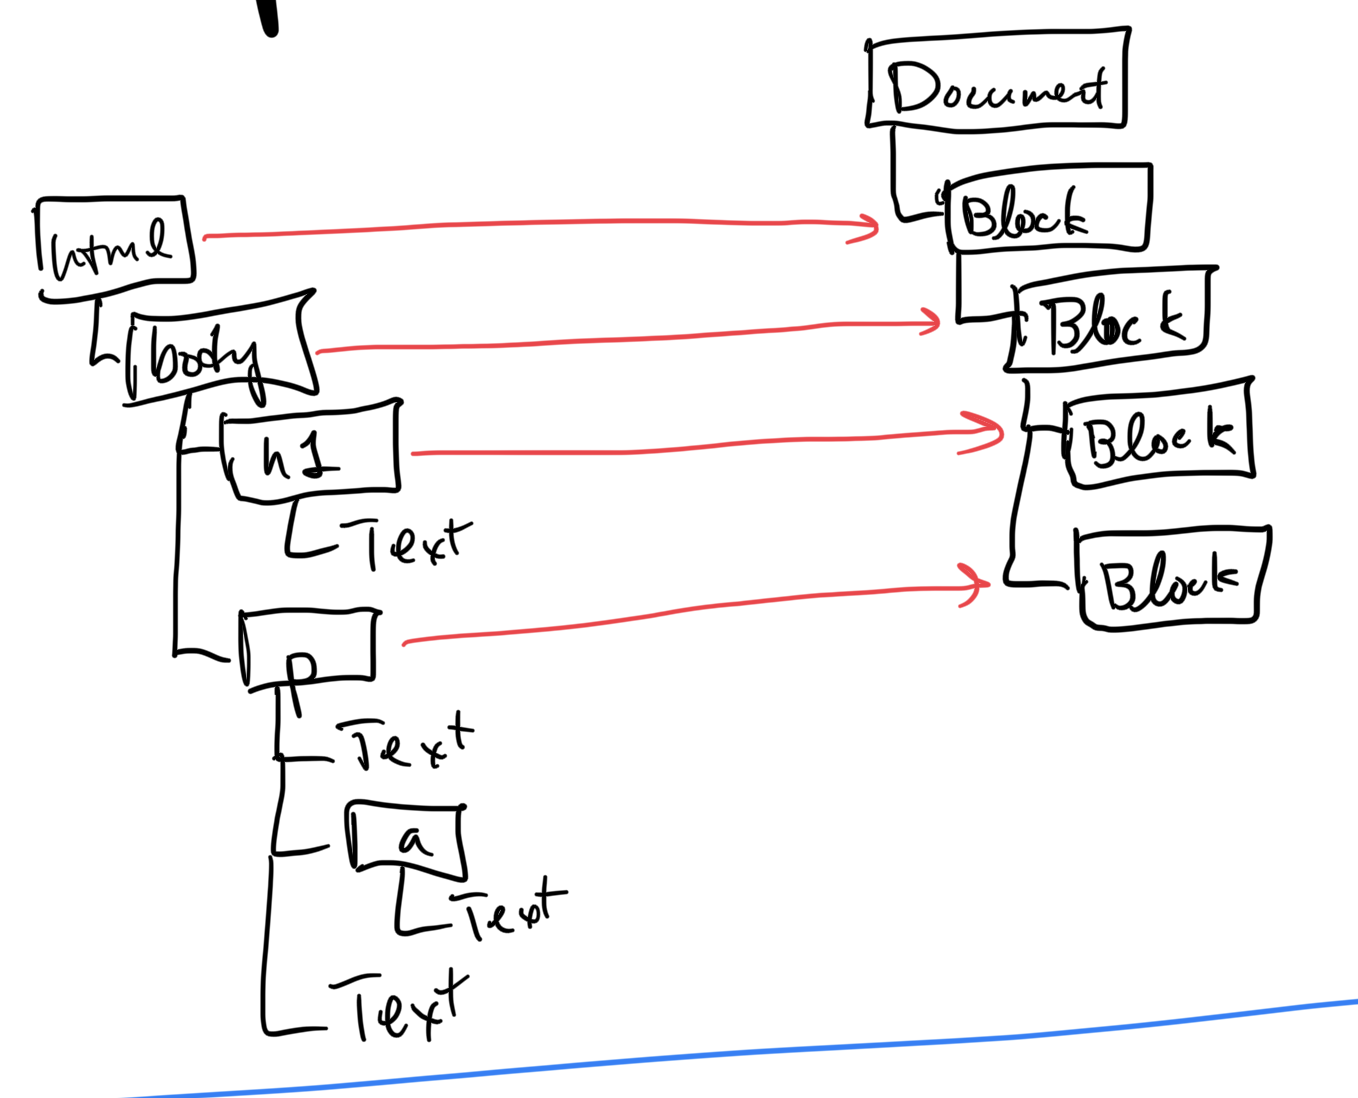
\includegraphics{im/layout-tree.png}
\caption{An example of an HTML tree and the corresponding layout tree.}\label{fig:LayoutTree}
\end{figure}

\begin{bookblock}{further}
In CSS, the layout mode is set by the
\href{https://developer.mozilla.org/en-US/docs/Web/CSS/display}{\texttt{display}
property}. The oldest CSS layout modes, like \texttt{inline} and
\texttt{block}, are set on the children instead of the parent, which
leads to hiccups like
\href{https://developer.mozilla.org/en-US/docs/Web/CSS/Visual_formatting_model\#anonymous_boxes}{anonymous
block boxes}. Newer properties like \texttt{inline-block},
\texttt{flex}, and \texttt{grid} are set on the parent, which avoids
this kind of error.
\end{bookblock}

\hypertarget{size-and-position}{%
\section{Size and Position}\label{size-and-position}}

In the {previous chapter}, the \texttt{Layout} object was
responsible for the whole web page, so it just laid out its content
starting at the top of the page. Now that we have multiple
\texttt{BlockLayout} objects each containing a different paragraph of
text, we're going to need to do things a little differently, computing a
size and position for each layout object independently.

Let's add \texttt{x}, \texttt{y}, \texttt{width}, and \texttt{height}
fields for each layout object type:
\begin{Shaded}
\begin{Highlighting}[]
\KeywordTok{class}\NormalTok{ BlockLayout:}
    \KeywordTok{def} \FunctionTok{\_\_init\_\_}\NormalTok{(}\VariableTok{self}\NormalTok{, node, parent, previous):}
        \CommentTok{\# ...}
        \VariableTok{self}\NormalTok{.x }\OperatorTok{=} \VariableTok{None}
        \VariableTok{self}\NormalTok{.y }\OperatorTok{=} \VariableTok{None}
        \VariableTok{self}\NormalTok{.width }\OperatorTok{=} \VariableTok{None}
        \VariableTok{self}\NormalTok{.height }\OperatorTok{=} \VariableTok{None}
\end{Highlighting}
\end{Shaded}
Do the same for \texttt{DocumentLayout}. Now we need to update the
\texttt{layout} method to use these fields.

Let's start with \texttt{cursor\_x} and \texttt{cursor\_y}. Instead of
having them denote absolute positions on the page, let's make them
relative to the \texttt{BlockLayout}'s \texttt{x} and \texttt{y}. So
they now need to start from \texttt{0} instead of \texttt{HSTEP} and
\texttt{VSTEP}, in both \texttt{layout} and \texttt{flush}:
\begin{Shaded}
\begin{Highlighting}[]
\KeywordTok{class}\NormalTok{ BlockLayout:}
    \KeywordTok{def}\NormalTok{ layout(}\VariableTok{self}\NormalTok{):}
        \ControlFlowTok{else}\NormalTok{:}
            \VariableTok{self}\NormalTok{.cursor\_x }\OperatorTok{=} \DecValTok{0}
            \VariableTok{self}\NormalTok{.cursor\_y }\OperatorTok{=} \DecValTok{0}

    \KeywordTok{def}\NormalTok{ flush(}\VariableTok{self}\NormalTok{):}
        \CommentTok{\# ...}
        \VariableTok{self}\NormalTok{.cursor\_x }\OperatorTok{=} \DecValTok{0}
        \CommentTok{\# ...}
\end{Highlighting}
\end{Shaded}

Since these fields are now relative, we'll need to add the block's
\texttt{x} and \texttt{y} position in \texttt{flush} when computing the
display list:
\begin{Shaded}
\begin{Highlighting}[]
\KeywordTok{class}\NormalTok{ BlockLayout:}
    \KeywordTok{def}\NormalTok{ flush(}\VariableTok{self}\NormalTok{):}
        \CommentTok{\# ...}
        \ControlFlowTok{for}\NormalTok{ rel\_x, word, font }\KeywordTok{in} \VariableTok{self}\NormalTok{.line:}
\NormalTok{            x }\OperatorTok{=} \VariableTok{self}\NormalTok{.x }\OperatorTok{+}\NormalTok{ rel\_x}
\NormalTok{            y }\OperatorTok{=} \VariableTok{self}\NormalTok{.y }\OperatorTok{+}\NormalTok{ baseline }\OperatorTok{{-}}\NormalTok{ font.metrics(}\StringTok{"ascent"}\NormalTok{)}
            \VariableTok{self}\NormalTok{.display\_list.append((x, y, word, font))}
        \CommentTok{\# ...}
\end{Highlighting}
\end{Shaded}

Similarly, to wrap lines, we can't compare \texttt{cursor\_x} to
\texttt{WIDTH}, because \texttt{cursor\_x} is a relative position while
\texttt{WIDTH} is an absolute position; instead, we'll wrap lines when
\texttt{cursor\_x} reaches the block's \texttt{width}:
\begin{Shaded}
\begin{Highlighting}[]
\KeywordTok{class}\NormalTok{ BlockLayout:}
    \KeywordTok{def}\NormalTok{ word(}\VariableTok{self}\NormalTok{, word):}
        \CommentTok{\# ...}
        \ControlFlowTok{if} \VariableTok{self}\NormalTok{.cursor\_x }\OperatorTok{+}\NormalTok{ w }\OperatorTok{\textgreater{}} \VariableTok{self}\NormalTok{.width:}
            \CommentTok{\# ...}
        \CommentTok{\# ...}
\end{Highlighting}
\end{Shaded}

So now that leaves us with the problem of computing these \texttt{x},
\texttt{y}, and \texttt{width} fields. Let's recall that
\texttt{BlockLayout}s represent blocks of text like paragraphs or
headings, and are stacked vertically one atop another. That means each
one starts at its parent's left edge and goes all the way across its
parent:\footnote{In the % \href{styles.md}{
  next chapter, we'll add
  support for author-defined styles, which in real browsers modify these
  layout rules by setting custom widths or changing how $x$ and $y$ positions are computed.}
\begin{Shaded}
\begin{Highlighting}[]
\KeywordTok{class}\NormalTok{ BlockLayout:}
    \KeywordTok{def}\NormalTok{ layout(}\VariableTok{self}\NormalTok{):}
        \VariableTok{self}\NormalTok{.x }\OperatorTok{=} \VariableTok{self}\NormalTok{.parent.x}
        \VariableTok{self}\NormalTok{.width }\OperatorTok{=} \VariableTok{self}\NormalTok{.parent.width}
        \CommentTok{\# ...}
\end{Highlighting}
\end{Shaded}

A layout object's vertical position depends on whether there's a
previous sibling. If there is one, the layout object starts right after
it; otherwise, it starts at its parent's top edge:
\begin{Shaded}
\begin{Highlighting}[]
\KeywordTok{class}\NormalTok{ BlockLayout:}
    \KeywordTok{def}\NormalTok{ layout(}\VariableTok{self}\NormalTok{):}
        \ControlFlowTok{if} \VariableTok{self}\NormalTok{.previous:}
            \VariableTok{self}\NormalTok{.y }\OperatorTok{=} \VariableTok{self}\NormalTok{.previous.y }\OperatorTok{+} \VariableTok{self}\NormalTok{.previous.height}
        \ControlFlowTok{else}\NormalTok{:}
            \VariableTok{self}\NormalTok{.y }\OperatorTok{=} \VariableTok{self}\NormalTok{.parent.y}
        \CommentTok{\# ...}
\end{Highlighting}
\end{Shaded}

Finally, height is a little tricky. A \texttt{BlockLayout} that contains
other blocks should be tall enough to contain all of its children, so
its height should be the sum of its children's heights:
\begin{Shaded}
\begin{Highlighting}[]
\KeywordTok{class}\NormalTok{ BlockLayout:}
    \KeywordTok{def}\NormalTok{ layout(}\VariableTok{self}\NormalTok{):}
        \CommentTok{\# ...}
        \ControlFlowTok{if}\NormalTok{ mode }\OperatorTok{==} \StringTok{"block"}\NormalTok{:}
            \VariableTok{self}\NormalTok{.height }\OperatorTok{=} \BuiltInTok{sum}\NormalTok{([}
\NormalTok{                child.height }\ControlFlowTok{for}\NormalTok{ child }\KeywordTok{in} \VariableTok{self}\NormalTok{.children])}
\end{Highlighting}
\end{Shaded}
However, a \texttt{BlockLayout} that contains text doesn't have
children; instead, it needs to be tall enough to contain all its text,
which we can conveniently read off from \texttt{cursor\_y}:\footnote{Since
  the height is just equal to \texttt{cursor\_y}, why not rename
  \texttt{cursor\_y} to \texttt{height} instead? You could, it would
  work fine, but I would rather not. As you can see from, say, the
  \texttt{y} computation, the \texttt{height} field is a public field,
  read by other layout objects to compute their positions. As such, I'd
  rather make sure it \emph{always} has the right value, whereas
  \texttt{cursor\_y} changes as we lay out a paragraph of text and
  therefore sometimes has the ``wrong'' value. Keeping these two fields
  separate avoids a whole class of nasty bugs where the \texttt{height}
  field is read ``too soon'' and therefore gets the wrong value.}
\begin{Shaded}
\begin{Highlighting}[]
\KeywordTok{class}\NormalTok{ BlockLayout:}
    \KeywordTok{def}\NormalTok{ layout(}\VariableTok{self}\NormalTok{):}
        \CommentTok{\# ...}
        \ControlFlowTok{else}\NormalTok{:}
            \VariableTok{self}\NormalTok{.height }\OperatorTok{=} \VariableTok{self}\NormalTok{.cursor\_y}
\end{Highlighting}
\end{Shaded}

These rules seem simple enough, but there's a subtlety here I have to
explain. Consider the \texttt{x} position. To compute a block's
\texttt{x} position, the \texttt{x} position of its parent block must
\emph{already} have been computed. So a block's \texttt{x} must
therefore be computed before its children's \texttt{x}. That means the
\texttt{x} computation has to go \emph{before} the recursive
\texttt{layout} call.

On the other hand, an element's \texttt{height} field depends on its
children's heights. So while \texttt{x} must be computed \emph{before}
the recursive call, \texttt{height} has to be computed \emph{after}.
Similarly, since the \texttt{y} position of a block depends on its
previous sibling's \texttt{y} position, the recursive \texttt{layout}
calls have to start at the first sibling and iterate through the list
forward.

That is, the \texttt{layout} method should perform its steps in this
order (see Figure~\ref{fig:LayoutOrder}):
\begin{enumerate}
%\tightlist
\item
  When \texttt{layout} is called, it first computes the \texttt{width},
  \texttt{x}, and \texttt{y} fields, reading from the \texttt{parent}
  and \texttt{previous} layout objects.
\item
  Next, it creates a child layout object for each child element.
\item
  Then, the child layout nodes are recursively laid out by calling their
  \texttt{layout} methods.
\item
  Finally, \texttt{layout} computes the \texttt{height} field, reading
  from the child layout objects.
\end{enumerate}

\begin{figure}[b!]
  \centering
\includegraphics[width=0.9\textwidth]{im/layout-order.png}
\caption{A flowchart showing how
  widths are computed top-down, from parent to child, while heights are
  computed bottom-up, from child to parent.}\label{fig:LayoutOrder}
\end{figure}

This kind of dependency reasoning is crucial to layout, and more broadly
to any kind of computation on trees. If you get the order of operations
wrong, some layout object will try to read a value that hasn't been
computed yet, and the browser will have a bug. We'll come back to this
issue of dependencies % \href{invalidation.md}{later}
in Chapter~\ref{ch:PreviousComputations}, where it will
become even more important.

\texttt{DocumentLayout} needs some layout code too, though since the
document always starts in the same place it's pretty simple:
\begin{Shaded}
\begin{Highlighting}[]
\KeywordTok{class}\NormalTok{ DocumentLayout:}
    \KeywordTok{def}\NormalTok{ layout(}\VariableTok{self}\NormalTok{):}
        \CommentTok{\# ...}
        \VariableTok{self}\NormalTok{.width }\OperatorTok{=}\NormalTok{ WIDTH }\OperatorTok{{-}} \DecValTok{2}\OperatorTok{*}\NormalTok{HSTEP}
        \VariableTok{self}\NormalTok{.x }\OperatorTok{=}\NormalTok{ HSTEP}
        \VariableTok{self}\NormalTok{.y }\OperatorTok{=}\NormalTok{ VSTEP}
\NormalTok{        child.layout()}
        \VariableTok{self}\NormalTok{.height }\OperatorTok{=}\NormalTok{ child.height}
\end{Highlighting}
\end{Shaded}
Note that there's some padding around the contents---\texttt{HSTEP} on
the left and right, and \texttt{VSTEP} above and below. That's so the
text won't run into the very edge of the window and get cut off.

Anyway, with all of the sizes and positions now computed correctly, our
browser should display all of the text on the page in the right places.

\begin{bookblock}{further}
Formally, computations on a tree like this can be described by an
\href{https://en.wikipedia.org/wiki/Attribute_grammar}{attribute
grammar}. Attribute grammar engines analyze dependencies between
different attributes to determine the right order to traverse the tree
and calculate each attribute.
\end{bookblock}

\hypertarget{recursive-painting}{%
\section{Recursive Painting}\label{recursive-painting}}

Our \texttt{layout} method is now doing quite a bit of work: computing
sizes and positions; creating child layout objects; recursively laying
out those child layout objects; and aggregating the display lists so the
text can be drawn to the screen. This is a bit messy, so let's take a
moment to extract just one part of this, the display list part. Along
the way, we can stop copying the display list contents over and over
again as we go up the layout tree.

I think it's most convenient to do that by adding a
\texttt{paint}\index{paint} function to each layout object, whose return
value is the display list entries for that object. Then there is a
separate function, \texttt{paint\_tree}, that recursively calls
\texttt{paint} on all layout objects:
\begin{Shaded}
\begin{Highlighting}[]
\KeywordTok{def}\NormalTok{ paint\_tree(layout\_object, display\_list):}
\NormalTok{    display\_list.extend(layout\_object.paint())}

    \ControlFlowTok{for}\NormalTok{ child }\KeywordTok{in}\NormalTok{ layout\_object.children:}
\NormalTok{        paint\_tree(child, display\_list)}
\end{Highlighting}
\end{Shaded}

For \texttt{DocumentLayout}, there is nothing to paint:
\begin{Shaded}
\begin{Highlighting}[]
\KeywordTok{class}\NormalTok{ DocumentLayout:}
    \KeywordTok{def}\NormalTok{ paint(}\VariableTok{self}\NormalTok{):}
        \ControlFlowTok{return}\NormalTok{ []}
\end{Highlighting}
\end{Shaded}
You can now delete the line that computes a \texttt{DocumentLayout}'s
\texttt{display\_list} field.

For a \texttt{BlockLayout} object, we need to copy over the
\texttt{display\_list} field that it computes during \texttt{recurse}
and \texttt{flush}:\footnote{And again, delete the line that computes a
  \texttt{BlockLayout}'s \texttt{display\_list} field by copying from
  child layout objects.}
\begin{Shaded}
\begin{Highlighting}[]
\KeywordTok{class}\NormalTok{ BlockLayout:}
    \KeywordTok{def}\NormalTok{ paint(}\VariableTok{self}\NormalTok{):}
        \ControlFlowTok{return} \VariableTok{self}\NormalTok{.display\_list}
\end{Highlighting}
\end{Shaded}

Now the browser can use \texttt{paint\_tree} to collect its own
\texttt{display\_list} variable:
\begin{Shaded}
\begin{Highlighting}[]
\KeywordTok{class}\NormalTok{ Browser:}
    \KeywordTok{def}\NormalTok{ load(}\VariableTok{self}\NormalTok{, url):}
        \CommentTok{\# ...}
        \VariableTok{self}\NormalTok{.display\_list }\OperatorTok{=}\NormalTok{ []}
\NormalTok{        paint\_tree(}\VariableTok{self}\NormalTok{.document, }\VariableTok{self}\NormalTok{.display\_list)}
        \VariableTok{self}\NormalTok{.draw()}
\end{Highlighting}
\end{Shaded}

Check it out: our browser is now using fancy tree-based layout! I
recommend pausing to test and debug. Tree-based layout is powerful but
complex, and we're about to add more features. Stable foundations make
for comfortable houses.

\begin{bookblock}{further}
Layout trees are common
\href{https://book.huihoo.com/debian-gnu-linux-desktop-survival-guide/Widget_Tree.html}{in
graphical user interface (GUI) frameworks}, but there are other ways to structure layout, such as
constraint-based layout. \TeX's
\href{https://www.overleaf.com/learn/latex/Articles/Boxes_and_Glue\%3A_A_Brief\%2C_but_Visual\%2C_Introduction_Using_LuaTeX}{boxes
and glue} and iOS's
\href{https://developer.apple.com/library/archive/documentation/UserExperience/Conceptual/AutolayoutPG/index.html}{auto-layout}
are two examples of this alternative paradigm.
\end{bookblock}

\hypertarget{backgrounds}{%
\section{Backgrounds}\label{backgrounds}}

Browsers use the layout tree a lot,\footnote{For example, in
%  \href{chrome.md}{
  Chapter~\ref{ch:ButtonsAndLinks}, % 7},
  we'll use the size and position of each
  link to figure out which one the user clicked on.} and one simple and
visually compelling use case is drawing backgrounds.

Backgrounds are rectangles, so our first task is putting rectangles in
the display list. Right now, the display list is a list of words to draw
to the screen, but we can conceptualize it instead as a list of
\emph{commands}, of which there is currently only one type. We now want two types
of commands:
\begin{Shaded}
\begin{Highlighting}[]
\KeywordTok{class}\NormalTok{ DrawText:}
    \KeywordTok{def} \FunctionTok{\_\_init\_\_}\NormalTok{(}\VariableTok{self}\NormalTok{, x1, y1, text, font):}
        \VariableTok{self}\NormalTok{.top }\OperatorTok{=}\NormalTok{ y1}
        \VariableTok{self}\NormalTok{.left }\OperatorTok{=}\NormalTok{ x1}
        \VariableTok{self}\NormalTok{.text }\OperatorTok{=}\NormalTok{ text}
        \VariableTok{self}\NormalTok{.font }\OperatorTok{=}\NormalTok{ font}
    
\KeywordTok{class}\NormalTok{ DrawRect:}
    \KeywordTok{def} \FunctionTok{\_\_init\_\_}\NormalTok{(}\VariableTok{self}\NormalTok{, x1, y1, x2, y2, color):}
        \VariableTok{self}\NormalTok{.top }\OperatorTok{=}\NormalTok{ y1}
        \VariableTok{self}\NormalTok{.left }\OperatorTok{=}\NormalTok{ x1}
        \VariableTok{self}\NormalTok{.bottom }\OperatorTok{=}\NormalTok{ y2}
        \VariableTok{self}\NormalTok{.right }\OperatorTok{=}\NormalTok{ x2}
        \VariableTok{self}\NormalTok{.color }\OperatorTok{=}\NormalTok{ color}
\end{Highlighting}
\end{Shaded}

Now \texttt{BlockLayout} must add \texttt{DrawText} objects for each
word it wants to draw, but only in inline mode:\footnote{Why not change
  the \texttt{display\_list} field inside a \texttt{BlockLayout} to
  contain \texttt{DrawText} commands directly? I suppose you could, but
  I think it's cleaner to create all of the draw commands in one place.}
\begin{Shaded}
\begin{Highlighting}[]
\KeywordTok{class}\NormalTok{ BlockLayout:}
    \KeywordTok{def}\NormalTok{ paint(}\VariableTok{self}\NormalTok{):}
\NormalTok{        cmds }\OperatorTok{=}\NormalTok{ []}
        \ControlFlowTok{if} \VariableTok{self}\NormalTok{.layout\_mode() }\OperatorTok{==} \StringTok{"inline"}\NormalTok{:}
            \ControlFlowTok{for}\NormalTok{ x, y, word, font }\KeywordTok{in} \VariableTok{self}\NormalTok{.display\_list:}
\NormalTok{                cmds.append(DrawText(x, y, word, font))}
        \ControlFlowTok{return}\NormalTok{ cmds}
\end{Highlighting}
\end{Shaded}

But it can also add a \texttt{DrawRect} command to draw a background.
Let's add a gray background to \texttt{pre} tags (which are used for
code examples):
\begin{Shaded}
\begin{Highlighting}[]
\KeywordTok{class}\NormalTok{ BlockLayout:}
    \KeywordTok{def}\NormalTok{ paint(}\VariableTok{self}\NormalTok{):}
        \CommentTok{\# ...}
        \ControlFlowTok{if} \BuiltInTok{isinstance}\NormalTok{(}\VariableTok{self}\NormalTok{.node, Element) }\KeywordTok{and} \VariableTok{self}\NormalTok{.node.tag }\OperatorTok{==} \StringTok{"pre"}\NormalTok{:}
\NormalTok{            x2, y2 }\OperatorTok{=} \VariableTok{self}\NormalTok{.x }\OperatorTok{+} \VariableTok{self}\NormalTok{.width, }\VariableTok{self}\NormalTok{.y }\OperatorTok{+} \VariableTok{self}\NormalTok{.height}
\NormalTok{            rect }\OperatorTok{=}\NormalTok{ DrawRect(}\VariableTok{self}\NormalTok{.x, }\VariableTok{self}\NormalTok{.y, x2, y2, }\StringTok{"gray"}\NormalTok{)}
\NormalTok{            cmds.append(rect)}
        \CommentTok{\# ...}
\end{Highlighting}
\end{Shaded}
Make sure this code comes \emph{before} the loop that adds
\texttt{DrawText} objects: the background has to be drawn \emph{below}
that text. Note also that \texttt{paint\_tree} calls \texttt{paint}
before recursing into the subtree, so the subtree also paints on top of
this background, as desired.

With the display list filled out, we need to \texttt{draw} each graphics
command. Let's add an \texttt{execute} method for this. On
\texttt{DrawText} it calls \texttt{create\_text}:
\begin{Shaded}
\begin{Highlighting}[]
\KeywordTok{class}\NormalTok{ DrawText:}
    \KeywordTok{def}\NormalTok{ execute(}\VariableTok{self}\NormalTok{, scroll, canvas):}
\NormalTok{        canvas.create\_text(}
            \VariableTok{self}\NormalTok{.left, }\VariableTok{self}\NormalTok{.top }\OperatorTok{{-}}\NormalTok{ scroll,}
\NormalTok{            text}\OperatorTok{=}\VariableTok{self}\NormalTok{.text,}
\NormalTok{            font}\OperatorTok{=}\VariableTok{self}\NormalTok{.font,}
\NormalTok{            anchor}\OperatorTok{=}\StringTok{\textquotesingle{}nw\textquotesingle{}}\NormalTok{)}
\end{Highlighting}
\end{Shaded}
Note that \texttt{execute} takes the scroll amount as a parameter; this
way, each graphics command does the relevant coordinate conversion
itself. \texttt{DrawRect} does the same with \texttt{create\_rectangle}:
\begin{Shaded}
\begin{Highlighting}[]
\KeywordTok{class}\NormalTok{ DrawRect:}
    \KeywordTok{def}\NormalTok{ execute(}\VariableTok{self}\NormalTok{, scroll, canvas):}
\NormalTok{        canvas.create\_rectangle(}
            \VariableTok{self}\NormalTok{.left, }\VariableTok{self}\NormalTok{.top }\OperatorTok{{-}}\NormalTok{ scroll,}
            \VariableTok{self}\NormalTok{.right, }\VariableTok{self}\NormalTok{.bottom }\OperatorTok{{-}}\NormalTok{ scroll,}
\NormalTok{            width}\OperatorTok{=}\DecValTok{0}\NormalTok{,}
\NormalTok{            fill}\OperatorTok{=}\VariableTok{self}\NormalTok{.color)}
\end{Highlighting}
\end{Shaded}
By default, \texttt{create\_rectangle} draws a one-pixel black border,
which we don't want for backgrounds, so make sure to pass
\texttt{width=0}.

We still want to skip offscreen graphics commands, so let's add a
\texttt{bottom} field to \texttt{DrawText} so we know when to skip
those:
\begin{Shaded}
\begin{Highlighting}[]
\KeywordTok{def} \FunctionTok{\_\_init\_\_}\NormalTok{(}\VariableTok{self}\NormalTok{, x1, y1, text, font):}
    \CommentTok{\# ...}
    \VariableTok{self}\NormalTok{.bottom }\OperatorTok{=}\NormalTok{ y1 }\OperatorTok{+}\NormalTok{ font.metrics(}\StringTok{"linespace"}\NormalTok{)}
\end{Highlighting}
\end{Shaded}
The browser's \texttt{draw} method now just uses \texttt{top} and
\texttt{bottom} to decide which commands to \texttt{execute}:
\begin{Shaded}
\begin{Highlighting}[]
\KeywordTok{class}\NormalTok{ Browser:}
    \KeywordTok{def}\NormalTok{ draw(}\VariableTok{self}\NormalTok{):}
        \VariableTok{self}\NormalTok{.canvas.delete(}\StringTok{"all"}\NormalTok{)}
        \ControlFlowTok{for}\NormalTok{ cmd }\KeywordTok{in} \VariableTok{self}\NormalTok{.display\_list:}
            \ControlFlowTok{if}\NormalTok{ cmd.top }\OperatorTok{\textgreater{}} \VariableTok{self}\NormalTok{.scroll }\OperatorTok{+}\NormalTok{ HEIGHT: }\ControlFlowTok{continue}
            \ControlFlowTok{if}\NormalTok{ cmd.bottom }\OperatorTok{\textless{}} \VariableTok{self}\NormalTok{.scroll: }\ControlFlowTok{continue}
\NormalTok{            cmd.execute(}\VariableTok{self}\NormalTok{.scroll, }\VariableTok{self}\NormalTok{.canvas)}
\end{Highlighting}
\end{Shaded}

Try your browser on a page---maybe
\href{https://browser.engineering/layout.html}{this one}---with code snippets on it.
You should see each code snippet set off with a gray background.

Here's one more cute benefit of tree-based layout: %. Thanks to tree-based layout
we now record the height of the whole page. The browser can use
that to avoid scrolling past the bottom:
\begin{Shaded}
\begin{Highlighting}[]
\KeywordTok{def}\NormalTok{ scrolldown(}\VariableTok{self}\NormalTok{, e):}
\NormalTok{    max\_y }\OperatorTok{=} \BuiltInTok{max}\NormalTok{(}\VariableTok{self}\NormalTok{.document.height }\OperatorTok{+} \DecValTok{2}\OperatorTok{*}\NormalTok{VSTEP }\OperatorTok{{-}}\NormalTok{ HEIGHT, }\DecValTok{0}\NormalTok{)}
    \VariableTok{self}\NormalTok{.scroll }\OperatorTok{=} \BuiltInTok{min}\NormalTok{(}\VariableTok{self}\NormalTok{.scroll }\OperatorTok{+}\NormalTok{ SCROLL\_STEP, max\_y)}
    \VariableTok{self}\NormalTok{.draw()}
\end{Highlighting}
\end{Shaded}
Note the \texttt{2*VSTEP}, to account for a \texttt{VSTEP} of whitespace
at the top and bottom of the page.

So those are the basics of tree-based layout! In fact, as we'll see in
the next two chapters, this is just one part of the layout tree's
central role in the browser. But before we get to that, we need to add
some styling capabilities to our browser. However, even with layout the
\href{https://browser.engineering}{browser.engineering} homepage looks a bit
better---see Figure~\ref{fig:BrowserEngineering3}.

% \begin{center}
\begin{figure}
  \centering
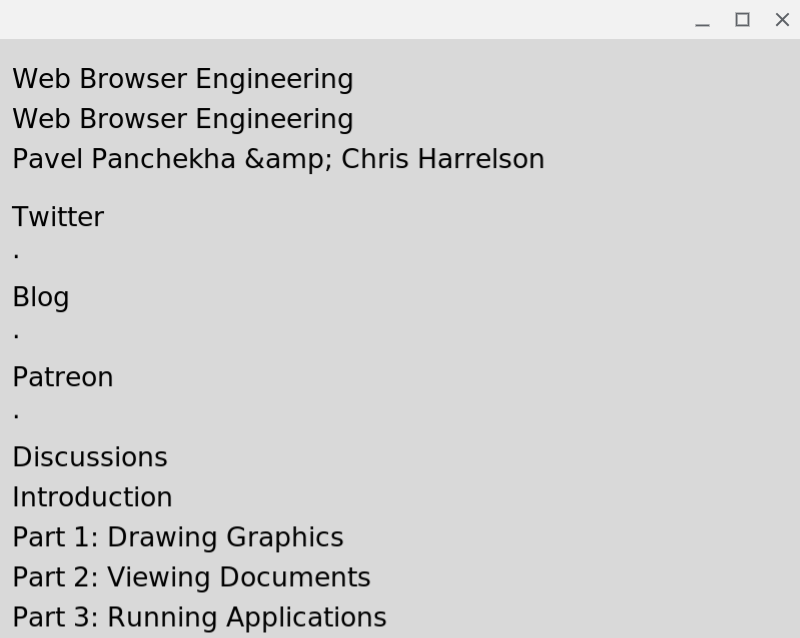
\includegraphics[width=0.8\textwidth]{examples/example5-browserengineering-screenshot.png}
\caption{\url{https://browser.engineering/index.html}
  viewed in this chapter's version of the browser.}\label{fig:BrowserEngineering3}
\end{figure}
%\end{center}

\begin{bookblock}{further}
The draft CSS
\href{https://developer.mozilla.org/en-US/docs/Web/API/CSS_Painting_API/Guide}{Painting
API} allows pages to extend the display list with new types of commands,
implemented in JavaScript. This makes it possible to use CSS for styling
with visually complex styling provided by a library.
\end{bookblock}

\hypertarget{summary}{%
\section{Summary}\label{LayingOutPages-summary}}

This chapter was a dramatic rewrite of our browser's layout engine:
\begin{itemize}
%\tightlist
\item
  Layout is now tree-based and produces a \emph{layout tree}.
\item
  Each node in the tree has one of two different \emph{layout modes}.
\item
  Layout computes a size and position for each layout object.
\item
  The display list now contains generic commands.
\item
  Plus, source code snippets now have backgrounds.
\end{itemize}
Tree-based layout makes it possible to dramatically expand our browser's
styling capabilities. We'll work on that in the % \href{styles.md}{
next chapter.

\hypertarget{outline}{%
\section{Outline}\label{LayingOutPages-outline}}

The complete set of functions, classes, and methods in our browser
should look something like this:

\begin{Shaded}
\begin{Highlighting}[]
\KeywordTok{class}\NormalTok{ URL:}
    \KeywordTok{def} \FunctionTok{\_\_init\_\_}\NormalTok{(url)}
    \KeywordTok{def}\NormalTok{ request()}
\NormalTok{WIDTH}
\NormalTok{HEIGHT}
\NormalTok{HSTEP}
\NormalTok{VSTEP}
\NormalTok{SCROLL\_STEP}
\NormalTok{FONTS}
\KeywordTok{def}\NormalTok{ get\_font(size, weight, slant)}
\KeywordTok{class}\NormalTok{ Text:}
    \KeywordTok{def} \FunctionTok{\_\_init\_\_}\NormalTok{(text, parent)}
    \KeywordTok{def} \FunctionTok{\_\_repr\_\_}\NormalTok{()}
\KeywordTok{class}\NormalTok{ Element:}
    \KeywordTok{def} \FunctionTok{\_\_init\_\_}\NormalTok{(tag, attributes, parent)}
    \KeywordTok{def} \FunctionTok{\_\_repr\_\_}\NormalTok{()}
\KeywordTok{def}\NormalTok{ print\_tree(node, indent)}
\KeywordTok{class}\NormalTok{ HTMLParser:}
    \KeywordTok{def} \FunctionTok{\_\_init\_\_}\NormalTok{(body)}
    \KeywordTok{def}\NormalTok{ parse()}
    \KeywordTok{def}\NormalTok{ get\_attributes(text)}
    \KeywordTok{def}\NormalTok{ add\_text(text)}
\NormalTok{    SELF\_CLOSING\_TAGS}
    \KeywordTok{def}\NormalTok{ add\_tag(tag)}
\NormalTok{    HEAD\_TAGS}
    \KeywordTok{def}\NormalTok{ implicit\_tags(tag)}
    \KeywordTok{def}\NormalTok{ finish()}
\KeywordTok{class}\NormalTok{ BlockLayout:}
    \KeywordTok{def} \FunctionTok{\_\_init\_\_}\NormalTok{(node, parent, previous)}
    \KeywordTok{def}\NormalTok{ token(tok)}
    \KeywordTok{def}\NormalTok{ word(word)}
    \KeywordTok{def}\NormalTok{ flush()}
    \KeywordTok{def}\NormalTok{ recurse(tree)}
    \KeywordTok{def}\NormalTok{ open\_tag(tag)}
    \KeywordTok{def}\NormalTok{ close\_tag(tag)}
    \KeywordTok{def}\NormalTok{ layout()}
    \KeywordTok{def}\NormalTok{ layout\_mode()}
    \KeywordTok{def}\NormalTok{ paint()}
\KeywordTok{class}\NormalTok{ Browser:}
    \KeywordTok{def} \FunctionTok{\_\_init\_\_}\NormalTok{()}
    \KeywordTok{def}\NormalTok{ load(url)}
    \KeywordTok{def}\NormalTok{ draw()}
    \KeywordTok{def}\NormalTok{ scrolldown(e)}
\NormalTok{BLOCK\_ELEMENTS}
\KeywordTok{class}\NormalTok{ DocumentLayout:}
    \KeywordTok{def} \FunctionTok{\_\_init\_\_}\NormalTok{(node)}
    \KeywordTok{def}\NormalTok{ layout()}
    \KeywordTok{def}\NormalTok{ paint()}
\KeywordTok{class}\NormalTok{ DrawText:}
    \KeywordTok{def} \FunctionTok{\_\_init\_\_}\NormalTok{(x1, y1, text, font)}
    \KeywordTok{def}\NormalTok{ execute(scroll, canvas)}
\KeywordTok{class}\NormalTok{ DrawRect:}
    \KeywordTok{def} \FunctionTok{\_\_init\_\_}\NormalTok{(x1, y1, x2, y2, color)}
    \KeywordTok{def}\NormalTok{ execute(scroll, canvas)}
\KeywordTok{def}\NormalTok{ paint\_tree(layout\_object, display\_list)}
\end{Highlighting}
\end{Shaded}

\hypertarget{exercises}{%
\section{Exercises}\label{LayingOutPages-exercises}}
\begin{enumerate}[label=\thechapter-\arabic*]
\item \emph{Links bar.} At the top and bottom of the web version of
  each chapter of this book there is
a gray bar naming the chapter and offering back and forward links. It is
enclosed in a \texttt{\textless{}nav\ class="links"\textgreater{}} tag.
Have your browser give this links bar the light gray background a real
browser would.

\item \emph{Hidden \texttt{head}.} There's a good chance your browser is still showing
scripts, styles, and page titles at the top of every page you visit.
Make it so that the \texttt{\textless{}head\textgreater{}} element and
its contents are never displayed. Those elements should still be in the
HTML tree, but not in the layout tree.

\item \emph{Bullets.} Add bullets to list items, which in HTML are
\texttt{\textless{}li\textgreater{}} tags. You can make them little
squares, located to the left of the list item itself. Also indent
\texttt{\textless{}li\textgreater{}} elements so the text inside the
element is to the right of the bullet point.

\item \emph{Table of contents.} The web version of this book has a table of contents at the top
of each chapter, enclosed in a
\texttt{\textless{}nav\ id="toc"\textgreater{}} tag, which contains a
list of links. Add the text ``Table of Contents'', with a gray
background, above that list. Don't modify the lexer or parser.

\item \emph{Anonymous block boxes.} Sometimes, an element has a mix of
text-like and container-like children. For example, in this HTML,
\begin{verbatim}
<div><i>Hello, </i><b>world!</b><p>So it began...</p></div>
\end{verbatim}
the \texttt{\textless{}div\textgreater{}} element has three children:
the \texttt{\textless{}i\textgreater{}},
\texttt{\textless{}b\textgreater{}}, and
\texttt{\textless{}p\textgreater{}} elements. The first two are
text-like; the last is container-like. This is supposed to look like two
paragraphs, one for the \texttt{\textless{}i\textgreater{}} and
\texttt{\textless{}b\textgreater{}} and the second for the
\texttt{\textless{}p\textgreater{}}. Make your browser do that.
Specifically, modify \texttt{BlockLayout} so it can be passed a sequence
of sibling nodes, instead of a single node. Then, modify the algorithm
that constructs the layout tree so that any sequence of text-like
elements gets made into a single \texttt{BlockLayout}.

\item \emph{Run-ins.} A ``run-in heading'' is a heading that is drawn as part
of the next paragraph's text.\footnote{The exercise names in this
  section could be considered run-in headings. But since browser support
  for the \texttt{display:\ run-in} property
  \href{https://caniuse.com/run-in}{is poor}, this book actually doesn't
  use it; the headings are actually embedded in the next paragraph.}
Modify your browser to render \texttt{\textless{}h6\textgreater{}}
elements as run-in headings. You'll need to implement the previous
exercise on anonymous block boxes, and then add a special case for
\texttt{\textless{}h6\textgreater{}} elements.
\end{enumerate}

\ifprintedoutput
\theendnotes
\setcounter{endnote}{0}
\fi

\chapter{Applying Author Styles}\label{ch:ApplyingAuthorStyles}
In the % \href{layout.md}{last chapter},
previous chapter we gave each \texttt{pre} element
a gray background. It looks OK, and it \emph{is} good to have defaults,
but sites want a say in how they look. Websites do that with
\emph{Cascading Style Sheets} (CSS), which allow web authors (and, as
we'll see, browser developers) to define how a web page ought to look.

\hypertarget{parsing-with-functions}{%
\section{Parsing with Functions}\label{parsing-with-functions}}

One way a web page can change its appearance is with the
\texttt{style}\index{style} attribute. For example, this changes an
element's background color:
\begin{bookblock*}{notcode}
\begin{Shaded}
\begin{Highlighting}[]
\NormalTok{\textless{}div style="background{-}color:lightblue"\textgreater{}\textless{}/div\textgreater{}}
\end{Highlighting}
\end{Shaded}
\end{bookblock*}
\noindent More generally, a \texttt{style} attribute contains property--value pairs
separated by semicolons. The browser looks at those
\href{https://developer.mozilla.org/en-US/docs/Web/CSS}{CSS}
property--value\index{CSS!property--value} pairs to determine how an
element looks, for example to determine its background color.

To add this to our browser, we'll need to start by
parsing\index{parsing} these property--value pairs. I'll use recursive
\emph{parsing functions}, which are a good way to build a complex parser
step by step. The idea is that each parsing function advances through
the text being parsed and returns the data it parsed. We'll have
different functions for different types of data, and organize them in a
\texttt{CSSParser} class that stores the text being parsed and the
parser's current position in it:
\begin{Shaded}
\begin{Highlighting}[]
\KeywordTok{class}\NormalTok{ CSSParser:}
    \KeywordTok{def} \FunctionTok{\_\_init\_\_}\NormalTok{(}\VariableTok{self}\NormalTok{, s):}
        \VariableTok{self}\NormalTok{.s }\OperatorTok{=}\NormalTok{ s}
        \VariableTok{self}\NormalTok{.i }\OperatorTok{=} \DecValTok{0}
\end{Highlighting}
\end{Shaded}

Let's start small and build up. A parsing function for whitespace
increments the index \texttt{i} past every whitespace character:
\begin{Shaded}
\begin{Highlighting}[]
\KeywordTok{def}\NormalTok{ whitespace(}\VariableTok{self}\NormalTok{):}
    \ControlFlowTok{while} \VariableTok{self}\NormalTok{.i }\OperatorTok{\textless{}} \BuiltInTok{len}\NormalTok{(}\VariableTok{self}\NormalTok{.s) }\KeywordTok{and} \VariableTok{self}\NormalTok{.s[}\VariableTok{self}\NormalTok{.i].isspace():}
        \VariableTok{self}\NormalTok{.i }\OperatorTok{+=} \DecValTok{1}
\end{Highlighting}
\end{Shaded}

Whitespace is meaningless, so there's no parsed data to return. But when
we parse property names, we'll want to return them:
\begin{Shaded}
\begin{Highlighting}[]
\KeywordTok{def}\NormalTok{ word(}\VariableTok{self}\NormalTok{):}
\NormalTok{    start }\OperatorTok{=} \VariableTok{self}\NormalTok{.i}
    \ControlFlowTok{while} \VariableTok{self}\NormalTok{.i }\OperatorTok{\textless{}} \BuiltInTok{len}\NormalTok{(}\VariableTok{self}\NormalTok{.s):}
        \ControlFlowTok{if} \VariableTok{self}\NormalTok{.s[}\VariableTok{self}\NormalTok{.i].isalnum() }\KeywordTok{or} \VariableTok{self}\NormalTok{.s[}\VariableTok{self}\NormalTok{.i] }\KeywordTok{in} \StringTok{"\#{-}.\%"}\NormalTok{:}
            \VariableTok{self}\NormalTok{.i }\OperatorTok{+=} \DecValTok{1}
        \ControlFlowTok{else}\NormalTok{:}
            \ControlFlowTok{break}
    \ControlFlowTok{if} \KeywordTok{not}\NormalTok{ (}\VariableTok{self}\NormalTok{.i }\OperatorTok{\textgreater{}}\NormalTok{ start):}
        \ControlFlowTok{raise} \PreprocessorTok{Exception}\NormalTok{(}\StringTok{"Parsing error"}\NormalTok{)}
    \ControlFlowTok{return} \VariableTok{self}\NormalTok{.s[start:}\VariableTok{self}\NormalTok{.i]}
\end{Highlighting}
\end{Shaded}
This function increments \texttt{i} through any word
characters,\footnote{I've chosen the set of word characters here to
  cover property names (which use letters and the dash), numbers (which
  use the minus sign, numbers, periods), units (the percent sign), and
  colors (which use the hash sign). Real CSS values have a more complex
  syntax but this is enough for our browser.} much like
\texttt{whitespace}. But to return the parsed data, it stores where it
started and extracts the substring it moved through.

Parsing functions can fail. The \texttt{word} function we just wrote
raises an exception if \texttt{i} hasn't advanced through at least one
character---otherwise it didn't point at a word to begin
with.\footnote{You can add error text to the exception-raising code,
  too; I recommend doing that to help you debug problems.} Likewise, to
check for a literal colon (or some other punctuation character) you'd do
this:
\begin{Shaded}
\begin{Highlighting}[]
\KeywordTok{def}\NormalTok{ literal(}\VariableTok{self}\NormalTok{, literal):}
    \ControlFlowTok{if} \KeywordTok{not}\NormalTok{ (}\VariableTok{self}\NormalTok{.i }\OperatorTok{\textless{}} \BuiltInTok{len}\NormalTok{(}\VariableTok{self}\NormalTok{.s) }\KeywordTok{and} \VariableTok{self}\NormalTok{.s[}\VariableTok{self}\NormalTok{.i] }\OperatorTok{==}\NormalTok{ literal):}
        \ControlFlowTok{raise} \PreprocessorTok{Exception}\NormalTok{(}\StringTok{"Parsing error"}\NormalTok{)}
    \VariableTok{self}\NormalTok{.i }\OperatorTok{+=} \DecValTok{1}
\end{Highlighting}
\end{Shaded}

The great thing about parsing functions is that they can build on one
another. For example, property--value pairs are a property, a colon, and
a value,\footnote{In reality, properties and values have different
  syntaxes, so using \texttt{word} for both isn't quite right, but for
  our browser's limited CSS implementation this simplification will do.} with
whitespace in between:
\begin{Shaded}
\begin{Highlighting}[]
\KeywordTok{def}\NormalTok{ pair(}\VariableTok{self}\NormalTok{):}
\NormalTok{    prop }\OperatorTok{=} \VariableTok{self}\NormalTok{.word()}
    \VariableTok{self}\NormalTok{.whitespace()}
    \VariableTok{self}\NormalTok{.literal(}\StringTok{":"}\NormalTok{)}
    \VariableTok{self}\NormalTok{.whitespace()}
\NormalTok{    val }\OperatorTok{=} \VariableTok{self}\NormalTok{.word()}
    \ControlFlowTok{return}\NormalTok{ prop.casefold(), val}
\end{Highlighting}
\end{Shaded}

We can parse sequences by calling parsing functions in a loop. For
example, \texttt{style} attributes are a sequence of property--value
pairs:
\begin{Shaded}
\begin{Highlighting}[]
\KeywordTok{def}\NormalTok{ body(}\VariableTok{self}\NormalTok{):}
\NormalTok{    pairs }\OperatorTok{=}\NormalTok{ \{\}}
    \ControlFlowTok{while} \VariableTok{self}\NormalTok{.i }\OperatorTok{\textless{}} \BuiltInTok{len}\NormalTok{(}\VariableTok{self}\NormalTok{.s):}
\NormalTok{        prop, val }\OperatorTok{=} \VariableTok{self}\NormalTok{.pair()}
\NormalTok{        pairs[prop.casefold()] }\OperatorTok{=}\NormalTok{ val}
        \VariableTok{self}\NormalTok{.whitespace()}
        \VariableTok{self}\NormalTok{.literal(}\StringTok{";"}\NormalTok{)}
        \VariableTok{self}\NormalTok{.whitespace()}
    \ControlFlowTok{return}\NormalTok{ pairs}
\end{Highlighting}
\end{Shaded}

Now, in a browser, we always have to think about handling errors.
Sometimes a web page author makes a mistake; sometimes our browser
doesn't support a feature some other browser does. So we should skip
property--value pairs that don't parse, but keep the ones that do.
We can skip things with this little function; it stops at any one of a
set of characters, and returns that character (or \texttt{None} if it
was stopped by the end of the file):
\begin{Shaded}
\begin{Highlighting}[]
\KeywordTok{def}\NormalTok{ ignore\_until(}\VariableTok{self}\NormalTok{, chars):}
    \ControlFlowTok{while} \VariableTok{self}\NormalTok{.i }\OperatorTok{\textless{}} \BuiltInTok{len}\NormalTok{(}\VariableTok{self}\NormalTok{.s):}
        \ControlFlowTok{if} \VariableTok{self}\NormalTok{.s[}\VariableTok{self}\NormalTok{.i] }\KeywordTok{in}\NormalTok{ chars:}
            \ControlFlowTok{return} \VariableTok{self}\NormalTok{.s[}\VariableTok{self}\NormalTok{.i]}
        \ControlFlowTok{else}\NormalTok{:}
            \VariableTok{self}\NormalTok{.i }\OperatorTok{+=} \DecValTok{1}
    \ControlFlowTok{return} \VariableTok{None}
\end{Highlighting}
\end{Shaded}

When we fail to parse a property--value pair, we skip either to the next
semicolon or to the end of the string:
\begin{Shaded}
\begin{Highlighting}[]
\KeywordTok{def}\NormalTok{ body(}\VariableTok{self}\NormalTok{):}
    \CommentTok{\# ...}
    \ControlFlowTok{while} \VariableTok{self}\NormalTok{.i }\OperatorTok{\textless{}} \BuiltInTok{len}\NormalTok{(}\VariableTok{self}\NormalTok{.s):}
        \ControlFlowTok{try}\NormalTok{:}
            \CommentTok{\# ...}
        \ControlFlowTok{except} \PreprocessorTok{Exception}\NormalTok{:}
\NormalTok{            why }\OperatorTok{=} \VariableTok{self}\NormalTok{.ignore\_until([}\StringTok{";"}\NormalTok{])}
            \ControlFlowTok{if}\NormalTok{ why }\OperatorTok{==} \StringTok{";"}\NormalTok{:}
                \VariableTok{self}\NormalTok{.literal(}\StringTok{";"}\NormalTok{)}
                \VariableTok{self}\NormalTok{.whitespace()}
            \ControlFlowTok{else}\NormalTok{:}
                \ControlFlowTok{break}
    \CommentTok{\# ...}
\end{Highlighting}
\end{Shaded}
Skipping parse errors is a double-edged sword. It hides error messages,
making it harder for authors to debug their style sheets; it also makes
it harder to debug your parser.\footnote{I suggest removing the
  \texttt{try} block when debugging.} So in most programming situations
this ``catch-all'' error handling is a code smell.

But ``catch-all'' error handling has an unusual benefit on the web. The
web is an ecosystem of many browsers,\footnote{And an ecosystem of many
  browser versions, some of which haven't been written yet---but need to
  be supported as best we can.} which (for example) support different
kinds of property values.\footnote{Our browser does not support
  parentheses in property values, for example, which real browsers use
  for things like the \texttt{calc} and \texttt{url} functions.} CSS
that parses in one browser might not parse in another. With silent parse
errors, browsers just ignore stuff they don't understand, and web pages
mostly work in all of them. The principle (variously called ``Postel's
Law'',\footnote{After a line in the specification of TCP, written by Jon
  Postel.} the ``Digital Principle'',\footnote{After a similar idea in
  circuit design, where transistors must be non-linear to reduce analog
  noise.} or the ``Robustness Principle'') is: produce maximally
conformant output but accept even minimally conformant input.

\begin{bookblock}{further}
This parsing method is formally called recursive descent parsing for an
\href{https://en.wikipedia.org/wiki/LL_parser}{LL(1)} language. Parsers
that use this method can be \href{https://simdjson.org/}{really, really
fast}, at least if you put a lot of work into it. In a browser, faster
parsing means pages load faster.
\end{bookblock}

\hypertarget{the-style-attribute}{%
\section{\texorpdfstring{The \texttt{style}
Attribute}{The style Attribute}}\label{the-style-attribute}}

Now that the \texttt{style} attribute is parsed, we can use that parsed
information in the rest of the browser. Let's do that inside a
\texttt{style} function, which saves the parsed \texttt{style} attribute
in the node's \texttt{style} field:
\begin{Shaded}
\begin{Highlighting}[]
\KeywordTok{def}\NormalTok{ style(node):}
\NormalTok{    node.style }\OperatorTok{=}\NormalTok{ \{\}}
    \ControlFlowTok{if} \BuiltInTok{isinstance}\NormalTok{(node, Element) }\KeywordTok{and} \StringTok{"style"} \KeywordTok{in}\NormalTok{ node.attributes:}
\NormalTok{        pairs }\OperatorTok{=}\NormalTok{ CSSParser(node.attributes[}\StringTok{"style"}\NormalTok{]).body()}
        \ControlFlowTok{for} \BuiltInTok{property}\NormalTok{, value }\KeywordTok{in}\NormalTok{ pairs.items():}
\NormalTok{            node.style[}\BuiltInTok{property}\NormalTok{] }\OperatorTok{=}\NormalTok{ value}
\end{Highlighting}
\end{Shaded}
The method can recurse through the HTML tree to make sure each element
gets a style:
\begin{Shaded}
\begin{Highlighting}[]
\KeywordTok{def}\NormalTok{ style(node):}
    \CommentTok{\# ...}
    \ControlFlowTok{for}\NormalTok{ child }\KeywordTok{in}\NormalTok{ node.children:}
\NormalTok{        style(child)}
\end{Highlighting}
\end{Shaded}

Call \texttt{style} in the browser's \texttt{load} method, after parsing
the HTML but before doing layout. With the \texttt{style} information
stored on each element, the browser can consult it for styling
information during paint:
\begin{Shaded}
\begin{Highlighting}[]
\KeywordTok{class}\NormalTok{ BlockLayout:}
    \KeywordTok{def}\NormalTok{ paint(}\VariableTok{self}\NormalTok{):}
        \CommentTok{\# ...}
\NormalTok{        bgcolor }\OperatorTok{=} \VariableTok{self}\NormalTok{.node.style.get(}\StringTok{"background{-}color"}\NormalTok{,}
                                      \StringTok{"transparent"}\NormalTok{)}
        \ControlFlowTok{if}\NormalTok{ bgcolor }\OperatorTok{!=} \StringTok{"transparent"}\NormalTok{:}
\NormalTok{            x2, y2 }\OperatorTok{=} \VariableTok{self}\NormalTok{.x }\OperatorTok{+} \VariableTok{self}\NormalTok{.width, }\VariableTok{self}\NormalTok{.y }\OperatorTok{+} \VariableTok{self}\NormalTok{.height}
\NormalTok{            rect }\OperatorTok{=}\NormalTok{ DrawRect(}\VariableTok{self}\NormalTok{.x, }\VariableTok{self}\NormalTok{.y, x2, y2, bgcolor)}
\NormalTok{            cmds.append(rect)}
        \CommentTok{\# ...}
\end{Highlighting}
\end{Shaded}
I've removed the default gray background from \texttt{pre} elements for
now, but we'll put it back soon.

Open \href{https://browser.engineering/styles.html}{the web version of
this chapter} up in your browser to test your code: the code block at
the start of the chapter should now have a light blue background.

So this is one way web pages can change their appearance. And in the
early days of the web,\footnote{I'm talking Netscape 3. The late 1990s.}
something like this was the \emph{only} way. But honestly, it's a
pain---you need to set a \texttt{style} attribute on each element, and
if you change the style that's a lot of attributes to edit.
CSS\index{CSS} was invented to improve on this state of affairs:
\begin{itemize}
%\tightlist
\item
  One CSS file can consistently style many web pages at once.
\item
  One line of CSS can consistently style many elements at once.
\item
  CSS is future-proof and supports browsers with different features.
\end{itemize}
To achieve these goals, CSS extends the \texttt{style} attribute with
two related ideas: \emph{selectors}\index{CSS!selector} and
\emph{cascading}. Selectors describe which HTML elements a list of
property--value pairs apply to.\footnote{CSS rules can also be guarded by
  ``media queries'', which say that a rule should apply only in certain
  browsing environments (like only on mobile or only in landscape mode).
  Media queries are super-important for building sites that work across
  many devices, like reading this book on a phone. We'll meet them in
%  \href{accessibility.md}{Chapter 14}
  Chapter~\ref{ch:Accessible}.} The combination of the two is
called a \emph{rule}\index{CSS!rule}, as shown in Figure~\ref{fig:CSSRule}.

% \begin{center}

\begin{figure}
\centering
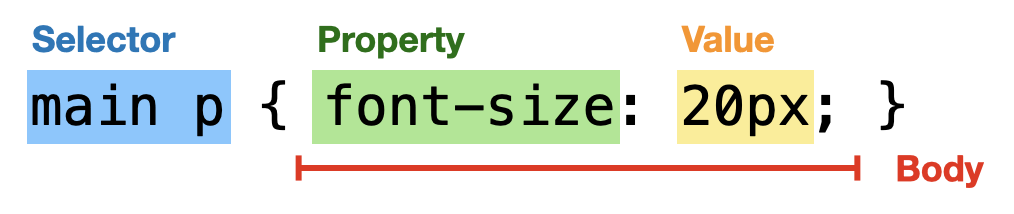
\includegraphics[width=0.8\textwidth]{im/styles-syntax.png}
\caption{An annotated CSS rule.}\label{fig:CSSRule}
\end{figure}

% \end{center}

Let's add support for CSS to our browser. We'll need to parse CSS files
into selectors and property--value pairs, figure out which elements on
the page match each selector, and copy those property values to the
elements' \texttt{style} fields.

\begin{bookblock}{further}
Actually, before CSS, you'd style pages with custom \emph{presentational
tags} like
\href{https://developer.mozilla.org/en-US/docs/Web/HTML/Element/font}{\texttt{font}}
and
\href{https://developer.mozilla.org/en-US/docs/Web/HTML/Element/center}{\texttt{center}}
(not to mention the \texttt{\textless{}b\textgreater{}} and
\texttt{\textless{}i\textgreater{}} tags we'll encounter later in this
chapter). This was easy to implement but made it hard to keep pages
consistent. There were also properties on
\texttt{\textless{}body\textgreater{}} like
\href{https://developer.mozilla.org/en-US/docs/Web/HTML/Element/body\#attributes}{\texttt{text}
and \texttt{vlink}} that could consistently set text colors, mainly for
links.
\end{bookblock}

\hypertarget{selectors}{%
\section{Selectors}\label{selectors}}

Selectors come in lots of types, but in our browser we'll support two:
tag selectors (\texttt{p} selects all
\texttt{\textless{}p\textgreater{}} elements, \texttt{ul} selects all
\texttt{\textless{}ul\textgreater{}} elements) and descendant selectors
(\texttt{article\ div} selects all \texttt{div} elements with an
\texttt{article} ancestor).\footnote{The descendant selector associates
  to the left; in other words, \texttt{a\ b\ c} means a \texttt{c} that
  descends from a \texttt{b} that descends from an \texttt{a}, which
  maybe you'd write \texttt{(a\ b)\ c} if CSS had parentheses.}

We'll have a class for each type of selector to store the selector's
contents, like the tag name for a tag selector:
\begin{Shaded}
\begin{Highlighting}[]
\KeywordTok{class}\NormalTok{ TagSelector:}
    \KeywordTok{def} \FunctionTok{\_\_init\_\_}\NormalTok{(}\VariableTok{self}\NormalTok{, tag):}
        \VariableTok{self}\NormalTok{.tag }\OperatorTok{=}\NormalTok{ tag}
\end{Highlighting}
\end{Shaded}
Each selector class will also test whether the selector matches an
element:
\begin{Shaded}
\begin{Highlighting}[]
\KeywordTok{class}\NormalTok{ TagSelector:}
    \KeywordTok{def}\NormalTok{ matches(}\VariableTok{self}\NormalTok{, node):}
        \ControlFlowTok{return} \BuiltInTok{isinstance}\NormalTok{(node, Element) }\KeywordTok{and} \VariableTok{self}\NormalTok{.tag }\OperatorTok{==}\NormalTok{ node.tag}
\end{Highlighting}
\end{Shaded}

A descendant selector works similarly. It has two parts, which are both
themselves selectors:
\begin{Shaded}
\begin{Highlighting}[]
\KeywordTok{class}\NormalTok{ DescendantSelector:}
    \KeywordTok{def} \FunctionTok{\_\_init\_\_}\NormalTok{(}\VariableTok{self}\NormalTok{, ancestor, descendant):}
        \VariableTok{self}\NormalTok{.ancestor }\OperatorTok{=}\NormalTok{ ancestor}
        \VariableTok{self}\NormalTok{.descendant }\OperatorTok{=}\NormalTok{ descendant}
\end{Highlighting}
\end{Shaded}
Then the \texttt{matches} method is recursive:
\begin{Shaded}
\begin{Highlighting}[]
\KeywordTok{class}\NormalTok{ DescendantSelector:}
    \KeywordTok{def}\NormalTok{ matches(}\VariableTok{self}\NormalTok{, node):}
        \ControlFlowTok{if} \KeywordTok{not} \VariableTok{self}\NormalTok{.descendant.matches(node): }\ControlFlowTok{return} \VariableTok{False}
        \ControlFlowTok{while}\NormalTok{ node.parent:}
            \ControlFlowTok{if} \VariableTok{self}\NormalTok{.ancestor.matches(node.parent): }\ControlFlowTok{return} \VariableTok{True}
\NormalTok{            node }\OperatorTok{=}\NormalTok{ node.parent}
        \ControlFlowTok{return} \VariableTok{False}
\end{Highlighting}
\end{Shaded}

Now, to create these selector objects, we need a parser. In this case,
that's just another parsing function:\footnote{Once again, using
  \texttt{word} here for tag names is actually not quite right, but it's
  close enough. One side effect of using \texttt{word} is that a class
  name selector (like \texttt{.main}) or an identifier selector (like
  \texttt{\#signup}) is mis-parsed as a tag name selector. But, luckily,
  that won't cause any harm since there aren't any elements with those
  tags.}
\begin{Shaded}
\begin{Highlighting}[]
\KeywordTok{class}\NormalTok{ CSSParser:}
    \KeywordTok{def}\NormalTok{ selector(}\VariableTok{self}\NormalTok{):}
\NormalTok{        out }\OperatorTok{=}\NormalTok{ TagSelector(}\VariableTok{self}\NormalTok{.word().casefold())}
        \VariableTok{self}\NormalTok{.whitespace()}
        \ControlFlowTok{while} \VariableTok{self}\NormalTok{.i }\OperatorTok{\textless{}} \BuiltInTok{len}\NormalTok{(}\VariableTok{self}\NormalTok{.s) }\KeywordTok{and} \VariableTok{self}\NormalTok{.s[}\VariableTok{self}\NormalTok{.i] }\OperatorTok{!=} \StringTok{"\{"}\NormalTok{:}
\NormalTok{            tag }\OperatorTok{=} \VariableTok{self}\NormalTok{.word()}
\NormalTok{            descendant }\OperatorTok{=}\NormalTok{ TagSelector(tag.casefold())}
\NormalTok{            out }\OperatorTok{=}\NormalTok{ DescendantSelector(out, descendant)}
            \VariableTok{self}\NormalTok{.whitespace()}
        \ControlFlowTok{return}\NormalTok{ out}
\end{Highlighting}
\end{Shaded}

A CSS file is just a sequence of selectors and blocks:
\begin{Shaded}
\begin{Highlighting}[]
\KeywordTok{def}\NormalTok{ parse(}\VariableTok{self}\NormalTok{):}
\NormalTok{    rules }\OperatorTok{=}\NormalTok{ []}
    \ControlFlowTok{while} \VariableTok{self}\NormalTok{.i }\OperatorTok{\textless{}} \BuiltInTok{len}\NormalTok{(}\VariableTok{self}\NormalTok{.s):}
        \VariableTok{self}\NormalTok{.whitespace()}
\NormalTok{        selector }\OperatorTok{=} \VariableTok{self}\NormalTok{.selector()}
        \VariableTok{self}\NormalTok{.literal(}\StringTok{"\{"}\NormalTok{)}
        \VariableTok{self}\NormalTok{.whitespace()}
\NormalTok{        body }\OperatorTok{=} \VariableTok{self}\NormalTok{.body()}
        \VariableTok{self}\NormalTok{.literal(}\StringTok{"\}"}\NormalTok{)}
\NormalTok{        rules.append((selector, body))}
    \ControlFlowTok{return}\NormalTok{ rules}
\end{Highlighting}
\end{Shaded}

Once again, let's pause to think about error handling. First, when we
call \texttt{body} while parsing CSS, we need it to stop when it reaches
a closing brace:
\begin{Shaded}
\begin{Highlighting}[]
\KeywordTok{def}\NormalTok{ body(}\VariableTok{self}\NormalTok{):}
    \CommentTok{\# ...}
    \ControlFlowTok{while} \VariableTok{self}\NormalTok{.i }\OperatorTok{\textless{}} \BuiltInTok{len}\NormalTok{(}\VariableTok{self}\NormalTok{.s) }\KeywordTok{and} \VariableTok{self}\NormalTok{.s[}\VariableTok{self}\NormalTok{.i] }\OperatorTok{!=} \StringTok{"\}"}\NormalTok{:}
        \ControlFlowTok{try}\NormalTok{:}
            \CommentTok{\# ...}
        \ControlFlowTok{except} \PreprocessorTok{Exception}\NormalTok{:}
\NormalTok{            why }\OperatorTok{=} \VariableTok{self}\NormalTok{.ignore\_until([}\StringTok{";"}\NormalTok{, }\StringTok{"\}"}\NormalTok{])}
            \ControlFlowTok{if}\NormalTok{ why }\OperatorTok{==} \StringTok{";"}\NormalTok{:}
                \VariableTok{self}\NormalTok{.literal(}\StringTok{";"}\NormalTok{)}
                \VariableTok{self}\NormalTok{.whitespace()}
            \ControlFlowTok{else}\NormalTok{:}
                \ControlFlowTok{break}
    \CommentTok{\# ...}
\end{Highlighting}
\end{Shaded}
Second, there might also be a parse error while parsing a selector. In
that case, we want to skip the whole rule:
\begin{Shaded}
\begin{Highlighting}[]
\KeywordTok{def}\NormalTok{ parse(}\VariableTok{self}\NormalTok{):}
    \CommentTok{\# ...}
    \ControlFlowTok{while} \VariableTok{self}\NormalTok{.i }\OperatorTok{\textless{}} \BuiltInTok{len}\NormalTok{(}\VariableTok{self}\NormalTok{.s):}
        \ControlFlowTok{try}\NormalTok{:}
            \CommentTok{\# ...}
        \ControlFlowTok{except} \PreprocessorTok{Exception}\NormalTok{:}
\NormalTok{            why }\OperatorTok{=} \VariableTok{self}\NormalTok{.ignore\_until([}\StringTok{"\}"}\NormalTok{])}
            \ControlFlowTok{if}\NormalTok{ why }\OperatorTok{==} \StringTok{"\}"}\NormalTok{:}
                \VariableTok{self}\NormalTok{.literal(}\StringTok{"\}"}\NormalTok{)}
                \VariableTok{self}\NormalTok{.whitespace()}
            \ControlFlowTok{else}\NormalTok{:}
                \ControlFlowTok{break}
    \CommentTok{\# ...}
\end{Highlighting}
\end{Shaded}

Error handling is hard to get right, so make sure to test your parser,
just like the HTML parser in Chapter~\ref{ch:DocumentTree}. %\href{html.md}{two chapters back}.
Here are
some errors you might run into:
\begin{itemize}
\item
  If the output is missing some rules or properties, it's probably a bug
  being hidden by error handling. Remove some \texttt{try} blocks and
  see if the error in question can be fixed.
\item
  If you're seeing extra rules or properties that are mangled versions
  of the correct ones, you probably forgot to update \texttt{i}
  somewhere.
\item
  If you're seeing an infinite loop, check whether the error-handling
  code always increases \texttt{i}. Each parsing function (except
  \texttt{whitespace}) should always increment \texttt{i}.
\end{itemize}
You can also add a \texttt{print} statement to the start and
end\footnote{If you print an open parenthesis at the start of the
  function and a close parenthesis at the end, you can use your editor's
  ``jump to other parenthesis'' feature to skip through output quickly.}
of each parsing function with the name of the parsing
function,\footnote{If you also add the right number of spaces to each
  line it'll be a lot easier to read. Don't neglect debugging niceties
  like this!} the index \texttt{i},\footnote{It can be especially
  helpful to print, say, the 20 characters around index \texttt{i} from
  the string.} and the parsed data. It's a lot of output, but it's a
sure-fire way to find really complicated bugs.

\begin{bookblock}{further}
A parser receives arbitrary bytes as input, so parser bugs are usually
easy for bad actors to exploit. Parser correctness is thus crucial to
browser security, as
\href{https://nvd.nist.gov/vuln/detail/CVE-2010-3971}{many}
\href{https://nvd.nist.gov/vuln/detail/CVE-2007-0943}{parser}
\href{https://nvd.nist.gov/vuln/detail/CVE-2010-1663}{bugs} have
demonstrated. Nowadays browser developers use
\href{https://hacks.mozilla.org/2021/02/browser-fuzzing-at-mozilla/}{fuzzing}
to try to find and fix such bugs.
\end{bookblock}

\hypertarget{applying-style-sheets}{%
\section{\texorpdfstring{Applying Style
Sheets\index{style!sheet}}{Applying Style Sheets}}\label{applying-style-sheets}}

With the parser debugged, the next step is applying the parsed style
sheet to the web page. Since each CSS rule can style many elements on
the page, this will require looping over all elements \emph{and} all
rules. When a rule applies, its property--value pairs are copied to the
element's style information:
\begin{Shaded}
\begin{Highlighting}[]
\KeywordTok{def}\NormalTok{ style(node, rules):}
    \CommentTok{\# ...}
    \ControlFlowTok{for}\NormalTok{ selector, body }\KeywordTok{in}\NormalTok{ rules:}
        \ControlFlowTok{if} \KeywordTok{not}\NormalTok{ selector.matches(node): }\ControlFlowTok{continue}
        \ControlFlowTok{for} \BuiltInTok{property}\NormalTok{, value }\KeywordTok{in}\NormalTok{ body.items():}
\NormalTok{            node.style[}\BuiltInTok{property}\NormalTok{] }\OperatorTok{=}\NormalTok{ value}
    \CommentTok{\# ...}
\end{Highlighting}
\end{Shaded}
Make sure to put this loop before the one that parses the \texttt{style}
attribute: the \texttt{style} attribute should override style sheet
values.

To try this out, we'll need a style sheet. Every browser ships with a
\emph{browser style sheet},\footnote{Technically called a ``User Agent''
  style sheet. User Agent, % \href{history.md}{
  like the Memex.} which
defines its default styling for the various HTML elements. For our
browser, it might look like this:
\begin{Shaded}
\begin{Highlighting}[]
\NormalTok{pre \{ }\KeywordTok{background{-}color}\CharTok{:} \ConstantTok{gray}\OperatorTok{;}\NormalTok{ \}}
\end{Highlighting}
\end{Shaded}
Let's store that in a new file, \texttt{browser.css}, and have our
browser read it when it starts:
\begin{Shaded}
\begin{Highlighting}[]
\NormalTok{DEFAULT\_STYLE\_SHEET }\OperatorTok{=}\NormalTok{ CSSParser(}\BuiltInTok{open}\NormalTok{(}\StringTok{"browser.css"}\NormalTok{).read()).parse()}
\end{Highlighting}
\end{Shaded}
Now, when the browser loads a web page, it can apply that default style
sheet to set up its default styling for each element:
\begin{Shaded}
\begin{Highlighting}[]
\KeywordTok{def}\NormalTok{ load(}\VariableTok{self}\NormalTok{, url):}
    \CommentTok{\# ...}
\NormalTok{    rules }\OperatorTok{=}\NormalTok{ DEFAULT\_STYLE\_SHEET.copy()}
\NormalTok{    style(}\VariableTok{self}\NormalTok{.nodes, rules)}
    \CommentTok{\# ...}
\end{Highlighting}
\end{Shaded}

The browser style sheet is the default for the whole web. But each web
site can also use CSS to set a consistent style for the whole site by
referencing CSS files using \texttt{link} elements:
\begin{bookblock*}{notcode}
\begin{Shaded}
\begin{Highlighting}[]
\NormalTok{\textless{}link rel="stylesheet" href="/main.css"\textgreater{}}
\end{Highlighting}
\end{Shaded}
\end{bookblock*}
\noindent The mandatory \texttt{rel} attribute identifies this link as a style
sheet\footnote{For browsers, \texttt{stylesheet} is the most important
  \href{https://developer.mozilla.org/en-US/docs/Web/HTML/Link_types}{kind
  of link}, but there's also \texttt{preload} for loading assets that a
  page will use later and \texttt{icon} for identifying favicons. Search
  engines also use these links; for example, \texttt{rel=canonical}
  names the ``true name'' of a page and search engines use it to track
  pages that appear at multiple URLs.} and the \texttt{href} attribute
has the style sheet URL. We need to find all these links, download their
style sheets, and apply them, as in Figure~\ref{fig:StyleSheet}.

\begin{figure}[tbp]
\centering
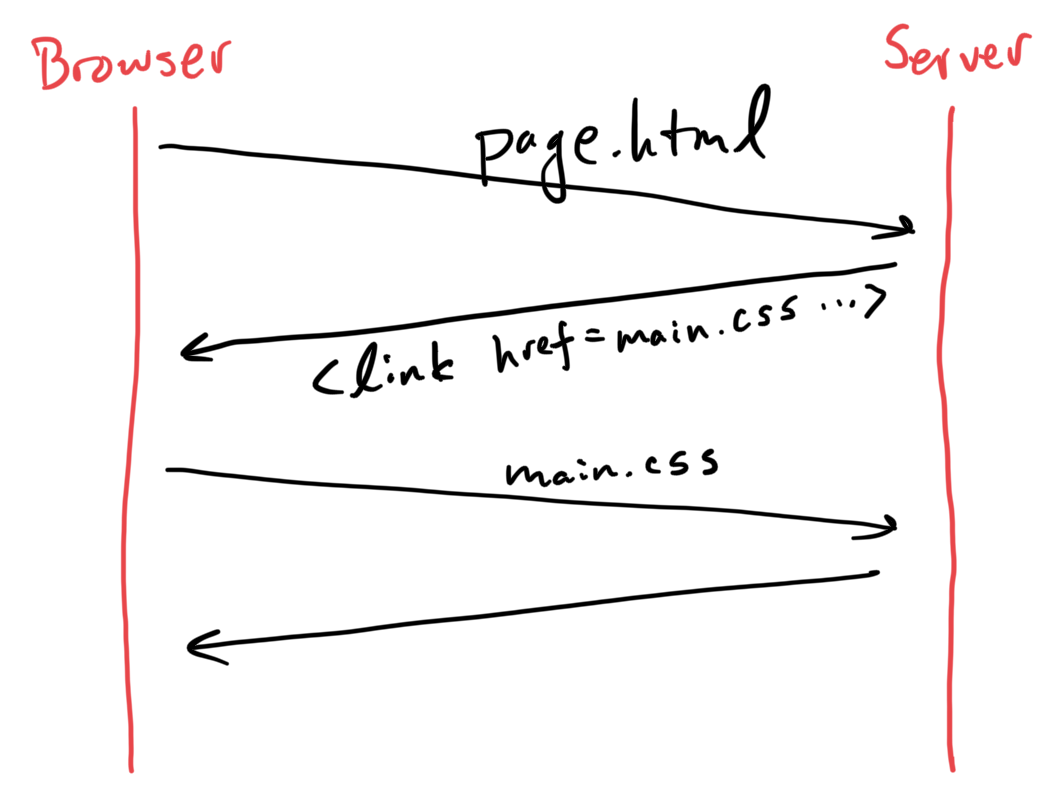
\includegraphics{im/styles-http.png}
\caption{A browser loading related assets, like a stylesheet, for a web page.}\label{fig:StyleSheet}
\end{figure}

Since we'll be doing similar tasks in the next few chapters, let's
generalize a bit and write a recursive function that turns a tree into a
list of nodes:
\begin{Shaded}
\begin{Highlighting}[]
\KeywordTok{def}\NormalTok{ tree\_to\_list(tree, }\BuiltInTok{list}\NormalTok{):}
    \BuiltInTok{list}\NormalTok{.append(tree)}
    \ControlFlowTok{for}\NormalTok{ child }\KeywordTok{in}\NormalTok{ tree.children:}
\NormalTok{        tree\_to\_list(child, }\BuiltInTok{list}\NormalTok{)}
    \ControlFlowTok{return} \BuiltInTok{list}
\end{Highlighting}
\end{Shaded}
I've written this helper to work on both HTML and layout trees, for
later. We can use \texttt{tree\_to\_list} with a Python list
comprehension to grab the URL of each linked style sheet:\footnote{It's
  kind of crazy, honestly, that Python lets you write things like
  this---crazy, but very convenient!}
\begin{Shaded}
\begin{Highlighting}[]
\KeywordTok{def}\NormalTok{ load(}\VariableTok{self}\NormalTok{, url):}
    \CommentTok{\# ...}
\NormalTok{    links }\OperatorTok{=}\NormalTok{ [node.attributes[}\StringTok{"href"}\NormalTok{]}
             \ControlFlowTok{for}\NormalTok{ node }\KeywordTok{in}\NormalTok{ tree\_to\_list(}\VariableTok{self}\NormalTok{.nodes, [])}
             \ControlFlowTok{if} \BuiltInTok{isinstance}\NormalTok{(node, Element)}
             \KeywordTok{and}\NormalTok{ node.tag }\OperatorTok{==} \StringTok{"link"}
             \KeywordTok{and}\NormalTok{ node.attributes.get(}\StringTok{"rel"}\NormalTok{) }\OperatorTok{==} \StringTok{"stylesheet"}
             \KeywordTok{and} \StringTok{"href"} \KeywordTok{in}\NormalTok{ node.attributes]}
    \CommentTok{\# ...}
\end{Highlighting}
\end{Shaded}

Now, these style sheet URLs are usually not full URLs; they are
something called \emph{relative URLs}, which can be:\footnote{There are
  other flavors, including query-relative and scheme-relative URLs, that
  I'm skipping.}
\begin{itemize}
%\tightlist
\item
  a normal URL, which specifies a scheme, host, path, and so on;
\item
  a host-relative URL, which starts with a slash but reuses the existing
  scheme and host; % or
\item
  a path-relative URL, which doesn't start with a slash and is resolved
  like a file name would be;
\item
  a scheme-relative URL that starts with ``\texttt{//}'' followed by a full URL,
  which should use the existing scheme.
\end{itemize}
To download the style sheets, we'll need to convert each relative URL
into a full URL:
\begin{Shaded}
\begin{Highlighting}[]
\KeywordTok{class}\NormalTok{ URL:}
    \KeywordTok{def}\NormalTok{ resolve(}\VariableTok{self}\NormalTok{, url):}
        \ControlFlowTok{if} \StringTok{"://"} \KeywordTok{in}\NormalTok{ url: }\ControlFlowTok{return}\NormalTok{ URL(url)}
        \ControlFlowTok{if} \KeywordTok{not}\NormalTok{ url.startswith(}\StringTok{"/"}\NormalTok{):}
            \BuiltInTok{dir}\NormalTok{, \_ }\OperatorTok{=} \VariableTok{self}\NormalTok{.path.rsplit(}\StringTok{"/"}\NormalTok{, }\DecValTok{1}\NormalTok{)}
\NormalTok{            url }\OperatorTok{=} \BuiltInTok{dir} \OperatorTok{+} \StringTok{"/"} \OperatorTok{+}\NormalTok{ url}
        \ControlFlowTok{if}\NormalTok{ url.startswith(}\StringTok{"//"}\NormalTok{):}
            \ControlFlowTok{return}\NormalTok{ URL(}\VariableTok{self}\NormalTok{.scheme }\OperatorTok{+} \StringTok{":"} \OperatorTok{+}\NormalTok{ url)}
        \ControlFlowTok{else}\NormalTok{:}
            \ControlFlowTok{return}\NormalTok{ URL(}\VariableTok{self}\NormalTok{.scheme }\OperatorTok{+} \StringTok{"://"} \OperatorTok{+} \VariableTok{self}\NormalTok{.host }\OperatorTok{+} \OperatorTok{\textbackslash{}}
                       \StringTok{":"} \OperatorTok{+} \BuiltInTok{str}\NormalTok{(}\VariableTok{self}\NormalTok{.port) }\OperatorTok{+}\NormalTok{ url)}
\end{Highlighting}
\end{Shaded}
Also, because of the early web architecture, browsers are responsible
for resolving parent directories (\texttt{..}) in relative URLs:
\begin{Shaded}
\begin{Highlighting}[]
\KeywordTok{class}\NormalTok{ URL:}
    \KeywordTok{def}\NormalTok{ resolve(}\VariableTok{self}\NormalTok{, url):}
        \ControlFlowTok{if} \KeywordTok{not}\NormalTok{ url.startswith(}\StringTok{"/"}\NormalTok{):}
            \BuiltInTok{dir}\NormalTok{, \_ }\OperatorTok{=} \VariableTok{self}\NormalTok{.path.rsplit(}\StringTok{"/"}\NormalTok{, }\DecValTok{1}\NormalTok{)}
            \ControlFlowTok{while}\NormalTok{ url.startswith(}\StringTok{"../"}\NormalTok{):}
\NormalTok{                \_, url }\OperatorTok{=}\NormalTok{ url.split(}\StringTok{"/"}\NormalTok{, }\DecValTok{1}\NormalTok{)}
                \ControlFlowTok{if} \StringTok{"/"} \KeywordTok{in} \BuiltInTok{dir}\NormalTok{:}
                    \BuiltInTok{dir}\NormalTok{, \_ }\OperatorTok{=} \BuiltInTok{dir}\NormalTok{.rsplit(}\StringTok{"/"}\NormalTok{, }\DecValTok{1}\NormalTok{)}
\NormalTok{            url }\OperatorTok{=} \BuiltInTok{dir} \OperatorTok{+} \StringTok{"/"} \OperatorTok{+}\NormalTok{ url}
\end{Highlighting}
\end{Shaded}

Now the browser can request each linked style sheet and add its rules to
the \texttt{rules} list:
\begin{Shaded}
\begin{Highlighting}[]
\KeywordTok{def}\NormalTok{ load(}\VariableTok{self}\NormalTok{, url):}
    \CommentTok{\# ...}
    \ControlFlowTok{for}\NormalTok{ link }\KeywordTok{in}\NormalTok{ links:}
\NormalTok{        style\_url }\OperatorTok{=}\NormalTok{ url.resolve(link)}
        \ControlFlowTok{try}\NormalTok{:}
\NormalTok{            body }\OperatorTok{=}\NormalTok{ style\_url.request()}
        \ControlFlowTok{except}\NormalTok{:}
            \ControlFlowTok{continue}
\NormalTok{        rules.extend(CSSParser(body).parse())}
\end{Highlighting}
\end{Shaded}
The \texttt{try}/\texttt{except} ignores style sheets that fail to
download, but it can also hide bugs in your code, so if something's not
right try removing it temporarily.

\begin{bookblock}{further}
Each browser engine has its own browser style sheet
(\href{https://source.chromium.org/chromium/chromium/src/+/master:third_party/blink/renderer/core/html/resources/html.css}{Chromium},
\href{https://github.com/WebKit/WebKit/blob/main/Source/WebCore/css/html.css}{WebKit},
\href{https://searchfox.org/mozilla-central/source/layout/style/res/html.css}{Gecko}).
\href{https://developer.mozilla.org/en-US/docs/Web/CSS/all}{Reset style
sheets} are often used to overcome any differences. This works because
web page style sheets take precedence over the browser style sheet, just
like in our browser, though real browsers
\href{https://www.w3.org/TR/2011/REC-CSS2-20110607/cascade.html\#cascading-order}{fiddle
with priorities}\index{cascade order} to make that happen.\footnotemark
\end{bookblock}
\footnotetext{
Our
  browser style sheet only has tag selectors in it, so just putting them
  first works well enough. But if the browser style sheet had any
  descendant selectors, we'd encounter bugs.
}

\hypertarget{cascading}{%
\section{Cascading}\label{cascading}}

A web page can now have any number of style sheets applied to it. And
since two rules can apply to the same element, rule order matters: it
determines which rules take priority, and when one rule overrides
another.

In CSS, the correct order is called \emph{cascade order}, and it is
based on the rule's selector, with file order as a tie breaker. This
system allows more specific rules to override more general ones, so that
you can have a browser style sheet, a site-wide style sheet, and maybe a
special style sheet for a specific web page, all co-existing.

Since our browser only has tag selectors, cascade order just counts
them:
\begin{Shaded}
\begin{Highlighting}[]
\KeywordTok{class}\NormalTok{ TagSelector:}
    \KeywordTok{def} \FunctionTok{\_\_init\_\_}\NormalTok{(}\VariableTok{self}\NormalTok{, tag):}
        \CommentTok{\# ...}
        \VariableTok{self}\NormalTok{.priority }\OperatorTok{=} \DecValTok{1}

\KeywordTok{class}\NormalTok{ DescendantSelector:}
    \KeywordTok{def} \FunctionTok{\_\_init\_\_}\NormalTok{(}\VariableTok{self}\NormalTok{, ancestor, descendant):}
        \CommentTok{\# ...}
        \VariableTok{self}\NormalTok{.priority }\OperatorTok{=}\NormalTok{ ancestor.priority }\OperatorTok{+}\NormalTok{ descendant.priority}
\end{Highlighting}
\end{Shaded}
Then cascade order for rules is just those priorities:
\begin{Shaded}
\begin{Highlighting}[]
\KeywordTok{def}\NormalTok{ cascade\_priority(rule):}
\NormalTok{    selector, body }\OperatorTok{=}\NormalTok{ rule}
    \ControlFlowTok{return}\NormalTok{ selector.priority}
\end{Highlighting}
\end{Shaded}

Now when we call \texttt{style}, we need to sort the rules, like this:
\begin{Shaded}
\begin{Highlighting}[]
\KeywordTok{def}\NormalTok{ load(}\VariableTok{self}\NormalTok{, url):}
    \CommentTok{\# ...}
\NormalTok{    style(}\VariableTok{self}\NormalTok{.nodes, }\BuiltInTok{sorted}\NormalTok{(rules, key}\OperatorTok{=}\NormalTok{cascade\_priority))}
    \CommentTok{\# ...}
\end{Highlighting}
\end{Shaded}
Note that before sorting \texttt{rules}, it is in file order. Python's
\texttt{sorted} function keeps the relative order of things with equal
priority, so file order acts as a tie breaker, as it should.

That's it: we've added CSS to our web browser! I mean---for background
colors. But there's more to web design than that. For example, if you're
changing background colors you might want to change foreground colors as
well---the CSS \texttt{color} property. But there's a catch:
\texttt{color} affects text, and there's no way to select a text node.
How can that work?

\begin{bookblock}{further}
Web pages can also supply
\href{https://developer.mozilla.org/en-US/docs/Web/CSS/Alternative_style_sheets}{alternative
style sheets}, and some browsers provide (obscure) methods to switch
from the default to an alternate style sheet. The CSS standard also
allows for \href{https://userstyles.org}{user styles} that set custom
style sheets for websites, with a priority
\href{https://www.w3.org/TR/css-cascade/\#cascade-origin}{between}
browser and website-provided style sheets.
\end{bookblock}

\hypertarget{inherited-styles}{%
\section{Inherited Styles}\label{inherited-styles}}

The way text styles work in CSS is called
\emph{inheritance}.\index{inheritance} Inheritance means that if some
node doesn't have a value for a certain property, it uses its parent's
value instead. That includes text nodes. Some properties are inherited
and some aren't; it depends on the property. Background color isn't
inherited, but text color and other font properties are.

Let's implement inheritance for four font properties:
\texttt{font-size}, \texttt{font-style} (for \texttt{italic}),
\texttt{font-weight} (for \texttt{bold}), and \texttt{color}:
\begin{Shaded}
\begin{Highlighting}[]
\NormalTok{INHERITED\_PROPERTIES }\OperatorTok{=}\NormalTok{ \{}
    \StringTok{"font{-}size"}\NormalTok{: }\StringTok{"16px"}\NormalTok{,}
    \StringTok{"font{-}style"}\NormalTok{: }\StringTok{"normal"}\NormalTok{,}
    \StringTok{"font{-}weight"}\NormalTok{: }\StringTok{"normal"}\NormalTok{,}
    \StringTok{"color"}\NormalTok{: }\StringTok{"black"}\NormalTok{,}
\NormalTok{\}}
\end{Highlighting}
\end{Shaded}
The values in this dictionary are each property's defaults. We'll then
add the actual inheritance code to the \texttt{style} function. It has
to come \emph{before} the other loops, since explicit rules should
override inheritance:
\begin{Shaded}
\begin{Highlighting}[]
\KeywordTok{def}\NormalTok{ style(node, rules):}
    \CommentTok{\# ...}
    \ControlFlowTok{for} \BuiltInTok{property}\NormalTok{, default\_value }\KeywordTok{in}\NormalTok{ INHERITED\_PROPERTIES.items():}
        \ControlFlowTok{if}\NormalTok{ node.parent:}
\NormalTok{            node.style[}\BuiltInTok{property}\NormalTok{] }\OperatorTok{=}\NormalTok{ node.parent.style[}\BuiltInTok{property}\NormalTok{]}
        \ControlFlowTok{else}\NormalTok{:}
\NormalTok{            node.style[}\BuiltInTok{property}\NormalTok{] }\OperatorTok{=}\NormalTok{ default\_value}
    \CommentTok{\# ...}
\end{Highlighting}
\end{Shaded}

Inheriting font size comes with a twist. Web pages can use percentages
as font sizes: \texttt{h1\ \{\ font-size:\ 150\%\ \}} makes headings
50\% bigger than the surrounding text. But what if you had, say, a
\texttt{code} element inside an \texttt{h1} tag---would that inherit the
\texttt{150\%} value for \texttt{font-size}? Surely it shouldn't be
another 50\% bigger than the rest of the heading text?
% So,
In fact, browsers resolve font size percentages to absolute pixel
units before those values are inherited; it's called a ``computed
style''.\index{computed style}\footnote{The full CSS standard is a bit
  more confusing: there are
  \href{https://www.w3.org/TR/CSS2/cascade.html\#value-stages}{specified,
  computed, used, and actual values}, and they affect lots of CSS
  properties besides \texttt{font-size}. But we're not implementing
  those other properties in this book.}
\begin{Shaded}
\begin{Highlighting}[]
\KeywordTok{def}\NormalTok{ style(node, rules):}
    \CommentTok{\# ...}
    \ControlFlowTok{if}\NormalTok{ node.style[}\StringTok{"font{-}size"}\NormalTok{].endswith(}\StringTok{"\%"}\NormalTok{):}
        \CommentTok{\# ...}

    \ControlFlowTok{for}\NormalTok{ child }\KeywordTok{in}\NormalTok{ node.children:}
\NormalTok{        style(child, rules)}
\end{Highlighting}
\end{Shaded}

Resolving percentage sizes has just one tricky edge case: percentage
sizes for the root \texttt{html} element. In that case the percentage is
relative to the default font size:\footnote{This code has to parse and
  unparse font sizes because our \texttt{style} field stores strings; in
  a real browser the computed style is stored parsed so this doesn't
  have to happen.}
\begin{Shaded}
\begin{Highlighting}[]
\KeywordTok{def}\NormalTok{ style(node, rules):}
    \CommentTok{\# ...}
    \ControlFlowTok{if}\NormalTok{ node.style[}\StringTok{"font{-}size"}\NormalTok{].endswith(}\StringTok{"\%"}\NormalTok{):}
        \ControlFlowTok{if}\NormalTok{ node.parent:}
\NormalTok{            parent\_font\_size }\OperatorTok{=}\NormalTok{ node.parent.style[}\StringTok{"font{-}size"}\NormalTok{]}
        \ControlFlowTok{else}\NormalTok{:}
\NormalTok{            parent\_font\_size }\OperatorTok{=}\NormalTok{ INHERITED\_PROPERTIES[}\StringTok{"font{-}size"}\NormalTok{]}
\NormalTok{        node\_pct }\OperatorTok{=} \BuiltInTok{float}\NormalTok{(node.style[}\StringTok{"font{-}size"}\NormalTok{][:}\OperatorTok{{-}}\DecValTok{1}\NormalTok{]) }\OperatorTok{/} \DecValTok{100}
\NormalTok{        parent\_px }\OperatorTok{=} \BuiltInTok{float}\NormalTok{(parent\_font\_size[:}\OperatorTok{{-}}\DecValTok{2}\NormalTok{])}
\NormalTok{        node.style[}\StringTok{"font{-}size"}\NormalTok{] }\OperatorTok{=} \BuiltInTok{str}\NormalTok{(node\_pct }\OperatorTok{*}\NormalTok{ parent\_px) }\OperatorTok{+} \StringTok{"px"}
\end{Highlighting}
\end{Shaded}

Note that this happens after all of the different sources of style
values are handled (so we are working with the final \texttt{font-size}
value) but before we recurse (so any children can assume that their
parent's \texttt{font-size} has been resolved to a pixel value).

\begin{bookblock}{further}
Styling a page can be slow, so real browsers apply tricks like
\href{https://bugs.webkit.org/show_bug.cgi?id=53880}{bloom filters} for
descendant selectors,
\href{https://source.chromium.org/chromium/chromium/src/+/refs/tags/93.0.4532.3:third_party/blink/renderer/core/css/style-calculation.md}{indices}
for simple selectors, and various forms of
\href{https://hacks.mozilla.org/2017/08/inside-a-super-fast-css-engine-quantum-css-aka-stylo/}{sharing}
and
\href{https://blog.rust-lang.org/2017/11/14/Fearless-Concurrency-In-Firefox-Quantum.html}{parallelism}.
Some types of sharing are also important to reduce memory
usage---computed style sheets can be huge!
\end{bookblock}

\hypertarget{font-properties}{%
\section{Font Properties}\label{font-properties}}

So now with all these font properties implemented, let's change layout
to use them! That will let us move our default text styles to the
browser style sheet:
\begin{Shaded}
\begin{Highlighting}[]
\NormalTok{a \{ }\KeywordTok{color}\CharTok{:} \ConstantTok{blue}\OperatorTok{;}\NormalTok{ \}}
\NormalTok{i \{ }\KeywordTok{font{-}style}\CharTok{:} \DecValTok{italic}\OperatorTok{;}\NormalTok{ \}}
\NormalTok{b \{ }\KeywordTok{font{-}weight}\CharTok{:} \DecValTok{bold}\OperatorTok{;}\NormalTok{ \}}
\NormalTok{small \{ }\KeywordTok{font{-}size}\CharTok{:} \DecValTok{90}\DataTypeTok{\%}\OperatorTok{;}\NormalTok{ \}}
\NormalTok{big \{ }\KeywordTok{font{-}size}\CharTok{:} \DecValTok{110}\DataTypeTok{\%}\OperatorTok{;}\NormalTok{ \}}
\end{Highlighting}
\end{Shaded}

The browser looks up font information in \texttt{BlockLayout}'s
\texttt{word} method; we'll need to change it to use the node's
\texttt{style} field, and for that, we'll need to pass in the node
itself:
\begin{Shaded}
\begin{Highlighting}[]
\KeywordTok{class}\NormalTok{ BlockLayout:}
    \KeywordTok{def}\NormalTok{ recurse(}\VariableTok{self}\NormalTok{, node):}
        \ControlFlowTok{if} \BuiltInTok{isinstance}\NormalTok{(node, Text):}
            \ControlFlowTok{for}\NormalTok{ word }\KeywordTok{in}\NormalTok{ node.text.split():}
                \VariableTok{self}\NormalTok{.word(node, word)}
        \ControlFlowTok{else}\NormalTok{:}
            \CommentTok{\# ...}

    \KeywordTok{def}\NormalTok{ word(}\VariableTok{self}\NormalTok{, node, word):}
\NormalTok{        weight }\OperatorTok{=}\NormalTok{ node.style[}\StringTok{"font{-}weight"}\NormalTok{]}
\NormalTok{        style }\OperatorTok{=}\NormalTok{ node.style[}\StringTok{"font{-}style"}\NormalTok{]}
        \ControlFlowTok{if}\NormalTok{ style }\OperatorTok{==} \StringTok{"normal"}\NormalTok{: style }\OperatorTok{=} \StringTok{"roman"}
\NormalTok{        size }\OperatorTok{=} \BuiltInTok{int}\NormalTok{(}\BuiltInTok{float}\NormalTok{(node.style[}\StringTok{"font{-}size"}\NormalTok{][:}\OperatorTok{{-}}\DecValTok{2}\NormalTok{]) }\OperatorTok{*} \FloatTok{.75}\NormalTok{)}
\NormalTok{        font }\OperatorTok{=}\NormalTok{ get\_font(size, weight, style)}
        \CommentTok{\# ...}
\end{Highlighting}
\end{Shaded}
Note that for \texttt{font-style} we need to translate CSS ``normal'' to
Tk ``roman'' and for \texttt{font-size} we need to convert CSS pixels to
Tk points.

Text color requires a bit more plumbing. First, we have to read the
color and store it in the current \texttt{line}:
\begin{Shaded}
\begin{Highlighting}[]
\KeywordTok{def}\NormalTok{ word(}\VariableTok{self}\NormalTok{, node, word):}
\NormalTok{    color }\OperatorTok{=}\NormalTok{ node.style[}\StringTok{"color"}\NormalTok{]}
    \CommentTok{\# ...}
    \VariableTok{self}\NormalTok{.line.append((}\VariableTok{self}\NormalTok{.cursor\_x, word, font, color))}
    \CommentTok{\# ...}
\end{Highlighting}
\end{Shaded}
The \texttt{flush} method then copies it from \texttt{line} to
\texttt{display\_list}:
\begin{Shaded}
\begin{Highlighting}[]
\KeywordTok{def}\NormalTok{ flush(}\VariableTok{self}\NormalTok{):}
    \CommentTok{\# ...}
\NormalTok{    metrics }\OperatorTok{=}\NormalTok{ [font.metrics() }\ControlFlowTok{for}\NormalTok{ x, word, font, color }\KeywordTok{in} \VariableTok{self}\NormalTok{.line]}
    \CommentTok{\# ...}
    \ControlFlowTok{for}\NormalTok{ x, word, font, color }\KeywordTok{in} \VariableTok{self}\NormalTok{.line:}
        \CommentTok{\# ...}
        \VariableTok{self}\NormalTok{.display\_list.append((x, y, word, font, color))}
    \CommentTok{\# ...}
\end{Highlighting}
\end{Shaded}
That \texttt{display\_list} is converted to drawing commands in
\texttt{paint}:
\begin{Shaded}
\begin{Highlighting}[]
\KeywordTok{def}\NormalTok{ paint(}\VariableTok{self}\NormalTok{):}
    \CommentTok{\# ...}
    \ControlFlowTok{for}\NormalTok{ x, y, word, font, color }\KeywordTok{in} \VariableTok{self}\NormalTok{.display\_list:}
\NormalTok{        cmds.append(DrawText(}\VariableTok{self}\NormalTok{.x }\OperatorTok{+}\NormalTok{ x, }\VariableTok{self}\NormalTok{.y }\OperatorTok{+}\NormalTok{ y,}
\NormalTok{                                     word, font, color))}
\end{Highlighting}
\end{Shaded}
\texttt{DrawText} now needs a \texttt{color} argument, and needs to pass
it to \texttt{create\_text}'s \texttt{fill} parameter:
\begin{Shaded}
\begin{Highlighting}[]
\KeywordTok{class}\NormalTok{ DrawText:}
    \KeywordTok{def} \FunctionTok{\_\_init\_\_}\NormalTok{(}\VariableTok{self}\NormalTok{, x1, y1, text, font, color):}
        \CommentTok{\# ...}
        \VariableTok{self}\NormalTok{.color }\OperatorTok{=}\NormalTok{ color}

    \KeywordTok{def}\NormalTok{ execute(}\VariableTok{self}\NormalTok{, scroll, canvas):}
\NormalTok{        canvas.create\_text(}
            \CommentTok{\# ...}
\NormalTok{            fill}\OperatorTok{=}\VariableTok{self}\NormalTok{.color)}
\end{Highlighting}
\end{Shaded}

Phew! That was a lot of coordinated changes, so test everything and make
sure it works. You should now see links on the 
\href{https://browser.engineering/styles.html}{web version of this chapter} appear in
blue---and you might also notice that the rest of the text has become
slightly lighter.\footnote{The main body text on the web
  is colored \texttt{\#333}, or roughly 97\% black after
  \href{https://en.wikipedia.org/wiki/SRGB\#From_sRGB_to_CIE_XYZ}{gamma
  correction}.} Also, now that we're explicitly setting the text color,
we should explicitly set the background color as well:\footnote{My Linux
  machine sets the default background color to a light gray, while my
  macOS laptop has a ``Dark Mode'' where the default background color
  becomes a dark gray. Setting the background color explicitly avoids
  the browser looking strange in these situations.}
\begin{Shaded}
\begin{Highlighting}[]
\KeywordTok{class}\NormalTok{ Browser:}
    \KeywordTok{def} \FunctionTok{\_\_init\_\_}\NormalTok{(}\VariableTok{self}\NormalTok{):}
        \CommentTok{\# ...}
        \VariableTok{self}\NormalTok{.canvas }\OperatorTok{=}\NormalTok{ tkinter.Canvas(}
            \CommentTok{\# ...}
\NormalTok{            bg}\OperatorTok{=}\StringTok{"white"}\NormalTok{,}
\NormalTok{        )}
        \CommentTok{\# ...}
\end{Highlighting}
\end{Shaded}

These changes obsolete all the code in \texttt{BlockLayout} that handles
specific tags, like the \texttt{style}, \texttt{weight}, and
\texttt{size} properties and the \texttt{open\_tag} and
\texttt{close\_tag} methods. Let's refactor a bit to get rid of them:
\begin{Shaded}
\begin{Highlighting}[]
\KeywordTok{class}\NormalTok{ BlockLayout:}
    \KeywordTok{def}\NormalTok{ recurse(}\VariableTok{self}\NormalTok{, node):}
        \ControlFlowTok{if} \BuiltInTok{isinstance}\NormalTok{(node, Text):}
            \ControlFlowTok{for}\NormalTok{ word }\KeywordTok{in}\NormalTok{ node.text.split():}
                \VariableTok{self}\NormalTok{.word(node, word)}
        \ControlFlowTok{else}\NormalTok{:}
            \ControlFlowTok{if}\NormalTok{ node.tag }\OperatorTok{==} \StringTok{"br"}\NormalTok{:}
                \VariableTok{self}\NormalTok{.flush()}
            \ControlFlowTok{for}\NormalTok{ child }\KeywordTok{in}\NormalTok{ node.children:}
                \VariableTok{self}\NormalTok{.recurse(child)}
\end{Highlighting}
\end{Shaded}

Styling not only lets web page authors style their own web pages; it
also moves browser code to a simple style sheet. And that's a big
improvement: the style sheet is simpler and easier to edit. Sometimes
converting code to data like this means maintaining a new format, but
browsers get to reuse a format, CSS, they need to support anyway.

But of course our chapter also has the nice benefit of even better
rendering of this book's homepage (Figure~\ref{fig:BrowserEngineering4}).
Notice how the background is no
longer gray, and the links have colors.

%::: \{.center\}
\begin{figure}
  \centering
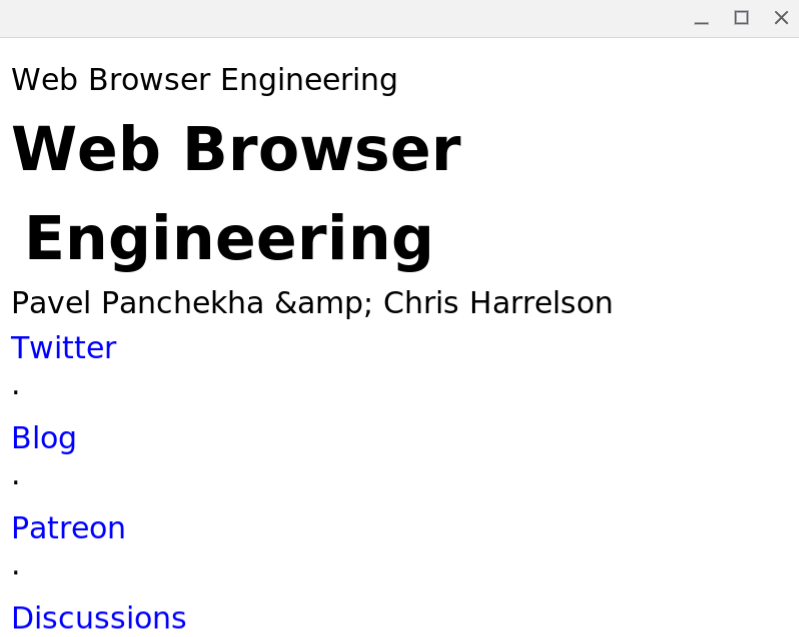
\includegraphics[width=0.8\textwidth]{examples/example6-browserengineering-screenshot.png}
\caption{\url{https://browser.engineering/index.html}
  viewed in this chapter's version of the browser.}\label{fig:BrowserEngineering4}
\end{figure}

\begin{bookblock}{further}
Usually a point is % one 72\textsuperscript{nd}
1/72 of an inch while pixel
size depends on the screen, but CSS instead
\href{https://www.w3.org/TR/2011/REC-CSS2-20110607/syndata.html\#length-units}{defines
an inch} as 96~pixels, because that was once a common screen resolution.
And these CSS pixels
\href{https://developer.mozilla.org/en-US/docs/Web/CSS/resolution}{need
not be} physical pixels! Seem weird? This complexity is the result of
changes in browsers (zooming) and hardware (high-DPI\footnotemark\ screens) plus the
need to be compatible with older web pages meant for the time when all
screens had 96~pixels per inch.
\end{bookblock}
\footnotetext{Dots per inch.}

\hypertarget{summary}{%
\section{Summary}\label{ApplyingAuthorStyles-summary}}

This chapter implemented a rudimentary but complete styling engine,
including downloading, parsing, matching, sorting, and applying CSS
files. That means we:
\begin{itemize}
%\tightlist
\item
  wrote a CSS parser;
\item
  added support for both \texttt{style} attributes and \texttt{link}ed
  CSS files;
\item
  implemented cascading and inheritance;
\item
  refactored \texttt{BlockLayout} to move the font properties to CSS;
\item
  moved most tag-specific reasoning to a browser style sheet.
\end{itemize}
Our styling engine is also relatively easy to extend with properties and
selectors.

\hypertarget{outline}{%
\section{Outline}\label{ApplyingAuthorStyles-outline}}

The complete set of functions, classes, and methods in our browser
should now look something like this:

\begin{Shaded}
\begin{Highlighting}[]
\KeywordTok{class}\NormalTok{ URL:}
    \KeywordTok{def} \FunctionTok{\_\_init\_\_}\NormalTok{(url)}
    \KeywordTok{def}\NormalTok{ request()}
    \KeywordTok{def}\NormalTok{ resolve(url)}
\NormalTok{WIDTH}
\NormalTok{HEIGHT}
\NormalTok{FONTS}
\KeywordTok{def}\NormalTok{ get\_font(size, weight, slant)}
\KeywordTok{class}\NormalTok{ Text:}
    \KeywordTok{def} \FunctionTok{\_\_init\_\_}\NormalTok{(text, parent)}
    \KeywordTok{def} \FunctionTok{\_\_repr\_\_}\NormalTok{()}
\KeywordTok{class}\NormalTok{ Element:}
    \KeywordTok{def} \FunctionTok{\_\_init\_\_}\NormalTok{(tag, attributes, parent)}
    \KeywordTok{def} \FunctionTok{\_\_repr\_\_}\NormalTok{()}
\KeywordTok{def}\NormalTok{ print\_tree(node, indent)}
\KeywordTok{class}\NormalTok{ HTMLParser:}
    \KeywordTok{def} \FunctionTok{\_\_init\_\_}\NormalTok{(body)}
    \KeywordTok{def}\NormalTok{ parse()}
    \KeywordTok{def}\NormalTok{ get\_attributes(text)}
    \KeywordTok{def}\NormalTok{ add\_text(text)}
\NormalTok{    SELF\_CLOSING\_TAGS}
    \KeywordTok{def}\NormalTok{ add\_tag(tag)}
\NormalTok{    HEAD\_TAGS}
    \KeywordTok{def}\NormalTok{ implicit\_tags(tag)}
    \KeywordTok{def}\NormalTok{ finish()}
\NormalTok{BLOCK\_ELEMENTS}
\KeywordTok{class}\NormalTok{ DrawRect:}
    \KeywordTok{def} \FunctionTok{\_\_init\_\_}\NormalTok{(x1, y1, x2, y2, color)}
    \KeywordTok{def}\NormalTok{ execute(scroll, canvas)}
\KeywordTok{class}\NormalTok{ DrawText:}
    \KeywordTok{def} \FunctionTok{\_\_init\_\_}\NormalTok{(x1, y1, text, font, color)}
    \KeywordTok{def}\NormalTok{ execute(scroll, canvas)}
\KeywordTok{def}\NormalTok{ paint\_tree(layout\_object, display\_list)}
\KeywordTok{class}\NormalTok{ BlockLayout:}
    \KeywordTok{def} \FunctionTok{\_\_init\_\_}\NormalTok{(node, parent, previous)}
    \KeywordTok{def}\NormalTok{ token(tok)}
    \KeywordTok{def}\NormalTok{ word(node, word)}
    \KeywordTok{def}\NormalTok{ flush()}
    \KeywordTok{def}\NormalTok{ recurse(node)}
    \KeywordTok{def}\NormalTok{ layout()}
    \KeywordTok{def}\NormalTok{ layout\_mode()}
    \KeywordTok{def}\NormalTok{ paint()}
\KeywordTok{class}\NormalTok{ DocumentLayout:}
    \KeywordTok{def} \FunctionTok{\_\_init\_\_}\NormalTok{(node)}
    \KeywordTok{def}\NormalTok{ layout()}
    \KeywordTok{def}\NormalTok{ paint()}
\KeywordTok{class}\NormalTok{ Browser:}
    \KeywordTok{def} \FunctionTok{\_\_init\_\_}\NormalTok{()}
    \KeywordTok{def}\NormalTok{ load(url)}
    \KeywordTok{def}\NormalTok{ draw()}
    \KeywordTok{def}\NormalTok{ scrolldown(e)}
\KeywordTok{def}\NormalTok{ tree\_to\_list(tree, }\NormalTok{list}\NormalTok{)}
\KeywordTok{class}\NormalTok{ CSSParser:}
    \KeywordTok{def} \FunctionTok{\_\_init\_\_}\NormalTok{(s)}
    \KeywordTok{def}\NormalTok{ whitespace()}
    \KeywordTok{def}\NormalTok{ literal(literal)}
    \KeywordTok{def}\NormalTok{ word()}
    \KeywordTok{def}\NormalTok{ pair()}
    \KeywordTok{def}\NormalTok{ ignore\_until(chars)}
    \KeywordTok{def}\NormalTok{ body()}
    \KeywordTok{def}\NormalTok{ selector()}
    \KeywordTok{def}\NormalTok{ parse()}
\KeywordTok{class}\NormalTok{ TagSelector:}
    \KeywordTok{def} \FunctionTok{\_\_init\_\_}\NormalTok{(tag)}
    \KeywordTok{def}\NormalTok{ matches(node)}
\KeywordTok{class}\NormalTok{ DescendantSelector:}
    \KeywordTok{def} \FunctionTok{\_\_init\_\_}\NormalTok{(ancestor, descendant)}
    \KeywordTok{def}\NormalTok{ matches(node)}
\NormalTok{INHERITED\_PROPERTIES}
\KeywordTok{def}\NormalTok{ style(node, rules)}
\KeywordTok{def}\NormalTok{ cascade\_priority(rule)}
\NormalTok{browser\_styles}
\NormalTok{DEFAULT\_STYLE\_SHEET}
\end{Highlighting}
\end{Shaded}

\hypertarget{exercises}{%
\section{Exercises}\label{ApplyingAuthorStyles-exercises}}
\begin{enumerate}[label=\thechapter-\arabic*]
\item\label{ex:font-family} \emph{Fonts.} Implement the \texttt{font-family} property, an
inheritable property that names which font should be used in an element.
Make text inside \texttt{\textless{}code\textgreater{}} elements use a
nice monospaced font like \texttt{Courier}. Beware the font cache.

\item\label{ex:WidthHeight} \emph{Width/height.} Add support for the \texttt{width} and
\texttt{height} properties to block layout. These can either be a pixel
value, which directly sets the width or height of the layout object, or
the word \texttt{auto}, in which case the existing layout algorithm is
used.

\item \emph{Class selectors.} Any HTML element can have a \texttt{class}
attribute, whose value is a space-separated list of that element's
classes. A CSS class selector, like \texttt{.main}, affects all elements
with the \texttt{main} class. Implement class selectors; give them
priority~10. If you've implemented them correctly, you should see syntax
highlighting for the code blocks in this book.

\item \emph{\texttt{display}.} Right now, the \texttt{layout\_mode} function relies on
a hard-coded list of block elements. In a real browser, the
\texttt{display} property controls this. Implement \texttt{display} with
a default value of \texttt{inline}, and move the list of block elements
to the browser style sheet.

\item \emph{Shorthand properties.} CSS ``shorthand properties'' set multiple
related CSS properties at the same time; for example,
\texttt{font:\ italic\ bold\ 100\%\ Times} sets the \texttt{font-style},
\texttt{font-weight}, \texttt{font-size}, and \texttt{font-family}
properties all at once. Add shorthand properties to your parser. (If you
haven't implemented \texttt{font-family} (Exercise~\ref{ex:font-family}),
just ignore that part.)

\item \emph{Inline style sheets.} The \texttt{link\ rel=stylesheet} syntax
allows importing an external style sheet (meaning one loaded via its own
HTTP request). There is also a way to provide a style sheet inline, as
part of the HTML, via the \texttt{\textless{}style\textgreater{}}
tag---everything up to the following
\texttt{\textless{}/style\textgreater{}} tag is interpreted as a style
sheet.\footnote{Both inline and external stylesheet apply in the order
  of their appearance in the HTML, though it might be easier to first
  implement inline style sheets applying after external ones.} Inline
style sheets are useful for creating self-contained example web pages,
but more importantly are a way that websites can load faster by
reducing the number of round-trip network requests to the server. Since
style sheets typically don't contain left angle brackets, you can
implement this feature without modifying the HTML parser.

\item \emph{Fast descendant selectors}: Right now, matching a selector like
\texttt{div\ div\ div\ div\ div} can take a long time---it's
$O(nd)$ in the worst case, where $n$ is the length of the
selector and $d$ is the depth of the layout tree. Modify the
descendant-selector matching code to run in $O(n)$ time. It may
help to have \texttt{DescendantSelector} store a list of base selectors
instead of just two.

\item \emph{Selector sequences.} Sometimes you want to select an element by
tag \emph{and} class. You do this by concatenating the selectors without
anything in between.\footnote{Not even whitespace!} For example,
\texttt{span.announce} selects elements that match both \texttt{span}
and \texttt{.announce}. Implement a new \texttt{SelectorSequence} class
to represent these and modify the parser to parse them. Sum
priorities.\footnote{Priorities for \texttt{SelectorSequence}s are
  supposed to compare the number of ID, class, and tag selectors in
  lexicographic order, but summing the priorities of the selectors in
  the sequence will work fine as long as no one strings more than ten
  selectors together.}

\item \emph{\texttt{!important}.} A CSS property--value pair can be marked ``important''
using the \texttt{!important} syntax, like this:
\begin{verbatim}
#banner a { color: black !important; }
\end{verbatim}
This gives that property--value pair (but not other pairs in the same
block!) a higher priority than any other selector (except for other
\texttt{!important} properties). Parse and implement \texttt{!important},
giving any property--value pairs marked this way a priority 10\,000 higher
than normal property--value pairs.

\item \emph{\texttt{:has} selectors.} The
\href{https://drafts.csswg.org/selectors-4/\#relational}{\texttt{:has}
selector} is the inverse of a descendant selector---it styles an
ancestor according to the presence of a descendant. Implement
\texttt{:has} selectors. Analyze the asymptotic speed of your
implementation. There is a clever implementation that is $O(1)$
amortized per element---can you find it?\footnote{In fact, browsers have
  to do something
  \href{https://blogs.igalia.com/blee/posts/2022/04/12/how-blink-tests-has-pseudo-class.html}{even
  more complex} to implement \texttt{:has} efficiently.}
\end{enumerate}

\ifprintedoutput
\theendnotes
\setcounter{endnote}{0}
\fi

\chapter{Handling Buttons and Links}\label{ch:ButtonsAndLinks}
Our browser is still missing the key insight of
\emph{hypertext}\index{hypertext}: documents linked together by
hyperlinks\index{hyperlink}. It lets us watch the waves, but not surf
the web. So in this chapter, we'll implement hyperlinks, an address bar,
and the rest of the browser interface---the part of the browser that
decides \emph{which} page we are looking at.

\hypertarget{where-are-the-links}{%
\section{Where Are The Links?}\label{where-are-the-links}}

The core of the web is the link, so the most important part of the
browser interface is clicking on links. But before we can quite get to
\emph{clicking} on links, we first need to answer a more fundamental
question: where on the screen \emph{are} the links? Though paragraphs
and headings have their sizes and positions recorded in the layout tree,
formatted text (like links) does not. We need to fix that.

The big idea is to introduce two new types of layout objects:
\texttt{LineLayout} and \texttt{TextLayout}. A \texttt{BlockLayout} will
now have a \texttt{LineLayout} child for each line of text, which itself
will contain a \texttt{TextLayout} for each word in that line. These new
classes can make the layout tree look different from the HTML tree. So
to avoid surprises, let's look at a simple example:
\begin{bookblock*}{notcode}
\begin{Shaded}
\begin{Highlighting}[]
\DataTypeTok{\textless{}}\KeywordTok{html}\DataTypeTok{\textgreater{}}
  \DataTypeTok{\textless{}}\KeywordTok{body}\DataTypeTok{\textgreater{}}
\NormalTok{    Here is some text that is}
    \DataTypeTok{\textless{}}\KeywordTok{br}\DataTypeTok{\textgreater{}}
\NormalTok{    spread across multiple lines}
  \DataTypeTok{\textless{}/}\KeywordTok{body}\DataTypeTok{\textgreater{}}
\DataTypeTok{\textless{}/}\KeywordTok{html}\DataTypeTok{\textgreater{}}
\end{Highlighting}
\end{Shaded}
\end{bookblock*}
\noindent The text in the \texttt{body} element wraps across two lines (because of
the \texttt{br} element), so the layout tree will have this structure:
\begin{bookblock*}{notcode}
\begin{verbatim}
DocumentLayout
  BlockLayout[block] (html element)
    BlockLayout[inline] (body element)
      LineLayout (first line of text)
        TextLayout ("Here")
        TextLayout ("is")
        TextLayout ("some")
        TextLayout ("text")
        TextLayout ("that")
        TextLayout ("is")
      LineLayout (second line of text)
        TextLayout ("spread")
        TextLayout ("across")
        TextLayout ("multiple")
        TextLayout ("lines")
\end{verbatim}
\end{bookblock*}
\noindent Note how one \texttt{body} element corresponds to a \texttt{BlockLayout}
with two \texttt{LineLayout}s inside, and how two text nodes turn into a
total of ten \texttt{TextLayout}s!

Let's get started. Defining \texttt{LineLayout} is straightforward:
\begin{Shaded}
\begin{Highlighting}[]
\KeywordTok{class}\NormalTok{ LineLayout:}
    \KeywordTok{def} \FunctionTok{\_\_init\_\_}\NormalTok{(}\VariableTok{self}\NormalTok{, node, parent, previous):}
        \VariableTok{self}\NormalTok{.node }\OperatorTok{=}\NormalTok{ node}
        \VariableTok{self}\NormalTok{.parent }\OperatorTok{=}\NormalTok{ parent}
        \VariableTok{self}\NormalTok{.previous }\OperatorTok{=}\NormalTok{ previous}
        \VariableTok{self}\NormalTok{.children }\OperatorTok{=}\NormalTok{ []}
\end{Highlighting}
\end{Shaded}
\texttt{TextLayout} is only a little more tricky. A single
\texttt{TextLayout} refers not to a whole HTML node but to a specific
word. That means \texttt{TextLayout} needs an extra argument to know
which word that is:
\begin{Shaded}
\begin{Highlighting}[]
\KeywordTok{class}\NormalTok{ TextLayout:}
    \KeywordTok{def} \FunctionTok{\_\_init\_\_}\NormalTok{(}\VariableTok{self}\NormalTok{, node, word, parent, previous):}
        \VariableTok{self}\NormalTok{.node }\OperatorTok{=}\NormalTok{ node}
        \VariableTok{self}\NormalTok{.word }\OperatorTok{=}\NormalTok{ word}
        \VariableTok{self}\NormalTok{.children }\OperatorTok{=}\NormalTok{ []}
        \VariableTok{self}\NormalTok{.parent }\OperatorTok{=}\NormalTok{ parent}
        \VariableTok{self}\NormalTok{.previous }\OperatorTok{=}\NormalTok{ previous}
\end{Highlighting}
\end{Shaded}
Like the other layout modes, \texttt{LineLayout} and \texttt{TextLayout}
will need their own \texttt{layout} and \texttt{paint} methods, but
before we get to those we need to think about how the
\texttt{LineLayout} and \texttt{TextLayout} objects will be created.
That has to happen during word wrapping.

Recall {how word wrapping happens (see Chapter 3)} inside
\texttt{BlockLayout}'s \texttt{word} method. That method updates a
\texttt{line} field, which stores all the words in the current line:
\begin{Shaded}
\begin{Highlighting}[]
\VariableTok{self}\NormalTok{.line.append((}\VariableTok{self}\NormalTok{.cursor\_x, word, font, color))}
\end{Highlighting}
\end{Shaded}
When it's time to go to the next line, \texttt{word} calls
\texttt{flush}, which computes the location of the line and each word in
it, and adds all the words to a \texttt{display\_list} field, which
stores all the words in the whole inline element. With
\texttt{TextLayout} and \texttt{LineLayout}, a lot of this complexity
goes away. The \texttt{LineLayout} can compute its own location in its
\texttt{layout} method, and instead of a \texttt{display\_list} field,
each \texttt{TextLayout} can just \texttt{paint} itself like normal. So
let's get started on this refactor.

Let's start with adding a word to a line. Instead of a \texttt{line}
field, we want to create \texttt{TextLayout} objects and add them to
\texttt{LineLayout} objects. The \texttt{LineLayout}s are children of
the \texttt{BlockLayout}, so the current line can be found at the end of
the \texttt{children} array:
\begin{Shaded}
\begin{Highlighting}[]
\KeywordTok{class}\NormalTok{ BlockLayout:}
    \KeywordTok{def}\NormalTok{ word(}\VariableTok{self}\NormalTok{, node, word):}
\NormalTok{        line }\OperatorTok{=} \VariableTok{self}\NormalTok{.children[}\OperatorTok{{-}}\DecValTok{1}\NormalTok{]}
\NormalTok{        previous\_word }\OperatorTok{=}\NormalTok{ line.children[}\OperatorTok{{-}}\DecValTok{1}\NormalTok{] }\ControlFlowTok{if}\NormalTok{ line.children }\ControlFlowTok{else} \VariableTok{None}
\NormalTok{        text }\OperatorTok{=}\NormalTok{ TextLayout(node, word, line, previous\_word)}
\NormalTok{        line.children.append(text)}
\end{Highlighting}
\end{Shaded}

Now let's think about what happens when we reach the end of the line.
The current code calls \texttt{flush}, which does stuff like positioning
text and clearing the \texttt{line} field. We don't want to do all
that---we just want to create a new \texttt{LineLayout} object. So let's
use a different method for that:
\begin{Shaded}
\begin{Highlighting}[]
\KeywordTok{class}\NormalTok{ BlockLayout:}
    \KeywordTok{def}\NormalTok{ word(}\VariableTok{self}\NormalTok{, node, word):}
        \ControlFlowTok{if} \VariableTok{self}\NormalTok{.cursor\_x }\OperatorTok{+}\NormalTok{ w }\OperatorTok{\textgreater{}} \VariableTok{self}\NormalTok{.width:}
            \VariableTok{self}\NormalTok{.new\_line()}
\end{Highlighting}
\end{Shaded}
This \texttt{new\_line} method just creates a new line and resets some
fields:
\begin{Shaded}
\begin{Highlighting}[]
\KeywordTok{class}\NormalTok{ BlockLayout:}
    \KeywordTok{def}\NormalTok{ new\_line(}\VariableTok{self}\NormalTok{):}
        \VariableTok{self}\NormalTok{.cursor\_x }\OperatorTok{=} \DecValTok{0}
\NormalTok{        last\_line }\OperatorTok{=} \VariableTok{self}\NormalTok{.children[}\OperatorTok{{-}}\DecValTok{1}\NormalTok{] }\ControlFlowTok{if} \VariableTok{self}\NormalTok{.children }\ControlFlowTok{else} \VariableTok{None}
\NormalTok{        new\_line }\OperatorTok{=}\NormalTok{ LineLayout(}\VariableTok{self}\NormalTok{.node, }\VariableTok{self}\NormalTok{, last\_line)}
        \VariableTok{self}\NormalTok{.children.append(new\_line)}
\end{Highlighting}
\end{Shaded}

Now there are a lot of fields we're not using. Let's clean them up. In the
core \texttt{layout} method, we don't need to initialize the
\texttt{display\_list}, \texttt{cursor\_y}, or \texttt{line} fields,
since we won't be using any of those any more. Instead, we just need to
call \texttt{new\_line} and \texttt{recurse}:
\begin{Shaded}
\begin{Highlighting}[]
\KeywordTok{class}\NormalTok{ BlockLayout:}
    \KeywordTok{def}\NormalTok{ layout(}\VariableTok{self}\NormalTok{):}
        \CommentTok{\# ...}
        \ControlFlowTok{else}\NormalTok{:}
            \VariableTok{self}\NormalTok{.new\_line()}
            \VariableTok{self}\NormalTok{.recurse(}\VariableTok{self}\NormalTok{.node)}
\end{Highlighting}
\end{Shaded}

The \texttt{layout} method already recurses into its children to lay
them out, so that part doesn't need any change. And moreover, we can now
compute the height of a paragraph of text by summing the height of its
lines, so this part of the code no longer needs to be different
depending on the layout mode:
\begin{Shaded}
\begin{Highlighting}[]
\KeywordTok{class}\NormalTok{ BlockLayout:}
    \KeywordTok{def}\NormalTok{ layout(}\VariableTok{self}\NormalTok{):}
        \CommentTok{\# ...}
        \VariableTok{self}\NormalTok{.height }\OperatorTok{=} \BuiltInTok{sum}\NormalTok{([child.height }\ControlFlowTok{for}\NormalTok{ child }\KeywordTok{in} \VariableTok{self}\NormalTok{.children])}
\end{Highlighting}
\end{Shaded}

You might also be tempted to delete the \texttt{flush} method, since
it's no longer called from anywhere. But keep it around for just a
moment---we'll need it to write the \texttt{layout} method for line and
text objects.

\begin{bookblock}{further}
The layout objects generated by a text node need not even be
consecutive. English containing a Farsi quotation, for example, can flip
from left-to-right to right-to-left in the middle of a line. The text
layout objects end up in a
\href{https://www.w3.org/International/articles/inline-bidi-markup/uba-basics}{surprising
order}. And then there are languages laid out
\href{https://en.wikipedia.org/wiki/Mongolian_script}{vertically}\ldots{}
\end{bookblock}

\hypertarget{line-layout-redux}{%
\section{Line Layout, Redux}\label{line-layout-redux}}

We're now creating line and text objects, but we still need to lay them
out. Let's start with lines. Lines stack vertically and take up their
parent's full width, so computing \texttt{x} and \texttt{y} and
\texttt{width} looks the same as for our other boxes:\footnote{You could
  reduce the duplication with some helper methods (or even something
  more elaborate, like mixin classes), but in a real browser different
  layout modes support different kinds of extra features (like text
  direction or margins) and the code looks quite different.}
\begin{Shaded}
\begin{Highlighting}[]
\KeywordTok{class}\NormalTok{ LineLayout:}
    \KeywordTok{def}\NormalTok{ layout(}\VariableTok{self}\NormalTok{):}
        \VariableTok{self}\NormalTok{.width }\OperatorTok{=} \VariableTok{self}\NormalTok{.parent.width}
        \VariableTok{self}\NormalTok{.x }\OperatorTok{=} \VariableTok{self}\NormalTok{.parent.x}

        \ControlFlowTok{if} \VariableTok{self}\NormalTok{.previous:}
            \VariableTok{self}\NormalTok{.y }\OperatorTok{=} \VariableTok{self}\NormalTok{.previous.y }\OperatorTok{+} \VariableTok{self}\NormalTok{.previous.height}
        \ControlFlowTok{else}\NormalTok{:}
            \VariableTok{self}\NormalTok{.y }\OperatorTok{=} \VariableTok{self}\NormalTok{.parent.y}
        
        \CommentTok{\# ...}
\end{Highlighting}
\end{Shaded}
Computing height, though, is different---this is where computing maximum
ascents, maximum descents, and so on comes in. Before we do that, let's
look at laying out \texttt{TextLayout}s.

To lay out text we need font metrics, so let's start by getting the
relevant font using the same font-construction code as
\texttt{BlockLayout}:
\begin{Shaded}
\begin{Highlighting}[]
\KeywordTok{class}\NormalTok{ TextLayout:}
    \KeywordTok{def}\NormalTok{ layout(}\VariableTok{self}\NormalTok{):}
\NormalTok{        weight }\OperatorTok{=} \VariableTok{self}\NormalTok{.node.style[}\StringTok{"font{-}weight"}\NormalTok{]}
\NormalTok{        style }\OperatorTok{=} \VariableTok{self}\NormalTok{.node.style[}\StringTok{"font{-}style"}\NormalTok{]}
        \ControlFlowTok{if}\NormalTok{ style }\OperatorTok{==} \StringTok{"normal"}\NormalTok{: style }\OperatorTok{=} \StringTok{"roman"}
\NormalTok{        size }\OperatorTok{=} \BuiltInTok{int}\NormalTok{(}\BuiltInTok{float}\NormalTok{(}\VariableTok{self}\NormalTok{.node.style[}\StringTok{"font{-}size"}\NormalTok{][:}\OperatorTok{{-}}\DecValTok{2}\NormalTok{]) }\OperatorTok{*} \FloatTok{.75}\NormalTok{)}
        \VariableTok{self}\NormalTok{.font }\OperatorTok{=}\NormalTok{ get\_font(size, weight, style)}
\end{Highlighting}
\end{Shaded}
Next, we need to compute the word's size and \texttt{x} position. We use the
font metrics to compute size, and stack words left to right to compute
position.
\begin{Shaded}
\begin{Highlighting}[]
\KeywordTok{class}\NormalTok{ TextLayout:}
    \KeywordTok{def}\NormalTok{ layout(}\VariableTok{self}\NormalTok{):}
        \CommentTok{\# ...}

        \VariableTok{self}\NormalTok{.width }\OperatorTok{=} \VariableTok{self}\NormalTok{.font.measure(}\VariableTok{self}\NormalTok{.word)}

        \ControlFlowTok{if} \VariableTok{self}\NormalTok{.previous:}
\NormalTok{            space }\OperatorTok{=} \VariableTok{self}\NormalTok{.previous.font.measure(}\StringTok{" "}\NormalTok{)}
            \VariableTok{self}\NormalTok{.x }\OperatorTok{=} \VariableTok{self}\NormalTok{.previous.x }\OperatorTok{+}\NormalTok{ space }\OperatorTok{+} \VariableTok{self}\NormalTok{.previous.width}
        \ControlFlowTok{else}\NormalTok{:}
            \VariableTok{self}\NormalTok{.x }\OperatorTok{=} \VariableTok{self}\NormalTok{.parent.x}

        \VariableTok{self}\NormalTok{.height }\OperatorTok{=} \VariableTok{self}\NormalTok{.font.metrics(}\StringTok{"linespace"}\NormalTok{)}
\end{Highlighting}
\end{Shaded}

There's no code here to compute the \texttt{y} position, however. The
vertical position of one word depends on the other words in the same
line, so we'll compute that \texttt{y} position inside
\texttt{LineLayout}'s \texttt{layout} method.\footnote{The \texttt{y}
  position could have been computed in \texttt{TextLayout}'s
  \texttt{layout} method---but then that layout method would have to
  come \emph{after} the baseline computation, not \emph{before}. Yet
  \texttt{font} must be computed \emph{before} the baseline computation.
  A real browser might resolve this paradox with multi-phase layout.
  There are many considerations and optimizations of this kind that are
  needed to make text layout super fast.}
That method will pilfer the code from the old \texttt{flush} method.
First, let's lay out each word:
\begin{Shaded}
\begin{Highlighting}[]
\KeywordTok{class}\NormalTok{ LineLayout:}
    \KeywordTok{def}\NormalTok{ layout(}\VariableTok{self}\NormalTok{):}
        \CommentTok{\# ...}
        \ControlFlowTok{for}\NormalTok{ word }\KeywordTok{in} \VariableTok{self}\NormalTok{.children:}
\NormalTok{            word.layout()}
\end{Highlighting}
\end{Shaded}
Next, we need to compute the line's baseline based on the maximum ascent
and descent, using basically the same code as the old \texttt{flush}
method:
\begin{Shaded}
\begin{Highlighting}[]
\CommentTok{\# ...}
\NormalTok{max\_ascent }\OperatorTok{=} \BuiltInTok{max}\NormalTok{([word.font.metrics(}\StringTok{"ascent"}\NormalTok{)}
                  \ControlFlowTok{for}\NormalTok{ word }\KeywordTok{in} \VariableTok{self}\NormalTok{.children])}
\NormalTok{baseline }\OperatorTok{=} \VariableTok{self}\NormalTok{.y }\OperatorTok{+} \FloatTok{1.25} \OperatorTok{*}\NormalTok{ max\_ascent}
\ControlFlowTok{for}\NormalTok{ word }\KeywordTok{in} \VariableTok{self}\NormalTok{.children:}
\NormalTok{    word.y }\OperatorTok{=}\NormalTok{ baseline }\OperatorTok{{-}}\NormalTok{ word.font.metrics(}\StringTok{"ascent"}\NormalTok{)}
\NormalTok{max\_descent }\OperatorTok{=} \BuiltInTok{max}\NormalTok{([word.font.metrics(}\StringTok{"descent"}\NormalTok{)}
                   \ControlFlowTok{for}\NormalTok{ word }\KeywordTok{in} \VariableTok{self}\NormalTok{.children])}
\end{Highlighting}
\end{Shaded}
Note that this code is reading from a \texttt{font} field on each word
and writing to each word's \texttt{y} field. That means that inside
\texttt{TextLayout}'s \texttt{layout} method, we need to compute
\texttt{x}, \texttt{width}, \texttt{height}, and \texttt{font},
but not \texttt{y}. Remember that for later.

Finally, since each line is now a standalone layout object, it needs to
have a height. We compute it from the maximum ascent and descent:
\begin{Shaded}
\begin{Highlighting}[]
\CommentTok{\# ...}
\VariableTok{self}\NormalTok{.height }\OperatorTok{=} \FloatTok{1.25} \OperatorTok{*}\NormalTok{ (max\_ascent }\OperatorTok{+}\NormalTok{ max\_descent)}
\end{Highlighting}
\end{Shaded}

So that's \texttt{layout} for \texttt{LineLayout} and
\texttt{TextLayout}. All that's left is painting. For
\texttt{LineLayout} there is nothing to paint:
\begin{Shaded}
\begin{Highlighting}[]
\KeywordTok{class}\NormalTok{ LineLayout:}
    \KeywordTok{def}\NormalTok{ paint(}\VariableTok{self}\NormalTok{):}
        \ControlFlowTok{return}\NormalTok{ []}
\end{Highlighting}
\end{Shaded}
And each \texttt{TextLayout} creates a single \texttt{DrawText} call:
\begin{Shaded}
\begin{Highlighting}[]
\KeywordTok{class}\NormalTok{ TextLayout:}
    \KeywordTok{def}\NormalTok{ paint(}\VariableTok{self}\NormalTok{):}
\NormalTok{        color }\OperatorTok{=} \VariableTok{self}\NormalTok{.node.style[}\StringTok{"color"}\NormalTok{]}
        \ControlFlowTok{return}\NormalTok{ [DrawText(}\VariableTok{self}\NormalTok{.x, }\VariableTok{self}\NormalTok{.y, }\VariableTok{self}\NormalTok{.word, }\VariableTok{self}\NormalTok{.font,}
        \ControlFlowTok{      }\NormalTok{           }\NormalTok{color)]}
\end{Highlighting}
\end{Shaded}
Now we don't need a \texttt{display\_list} field in
\texttt{BlockLayout}, and we can also remove the part of
\texttt{BlockLayout}'s \texttt{paint}\index{paint} that handles it.
Instead, \texttt{BlockLayout} can just recurse into its children and
paint them. So by adding \texttt{LineLayout} and \texttt{TextLayout} we
made \texttt{BlockLayout} quite a bit simpler and shared more code
between block and inline layout modes.

So, oof, well, this was quite a bit of refactoring. Take a moment to
test everything---it should look exactly identical to how it did before
we started this refactor. But while you can't see it, there's a crucial
difference: each blue link on the page now has an associated layout
object and its own size and position.

\begin{bookblock}{further}
Actually, text rendering is
\href{https://gankra.github.io/blah/text-hates-you/}{\emph{way} more
complex} than this.
\href{https://developer.apple.com/fonts/TrueType-Reference-Manual/RM06/Chap6morx.html}{Letters}
can transform and overlap, and the user might want to color certain
letters---or parts of letters---a different color. All of this is
possible in HTML, and real browsers do implement support for it.
\end{bookblock}

\hypertarget{click-handling}{%
\section{Click Handling}\label{click-handling}}

Now that we know where the links are, we can work on clicking them. In
Tk, click handling works just like key press handling: you bind an event
handler to a certain event. For click handling that event is
\texttt{\textless{}Button-1\textgreater{}}, button number~1 being the
left button on the mouse.\footnote{Button 2 is the middle button; button~3
  is the right-hand button.}
\begin{Shaded}
\begin{Highlighting}[]
\KeywordTok{class}\NormalTok{ Browser:}
    \KeywordTok{def} \FunctionTok{\_\_init\_\_}\NormalTok{(}\VariableTok{self}\NormalTok{):}
        \CommentTok{\# ...}
        \VariableTok{self}\NormalTok{.window.bind(}\StringTok{"\textless{}Button{-}1\textgreater{}"}\NormalTok{, }\VariableTok{self}\NormalTok{.click)}
\end{Highlighting}
\end{Shaded}

Inside \texttt{click}, we want to figure out what link the user has
clicked on. Luckily, the event handler is passed an event object, whose
\texttt{x} and \texttt{y} fields refer to where the click happened:
\begin{Shaded}
\begin{Highlighting}[]
\KeywordTok{class}\NormalTok{ Browser:}
    \KeywordTok{def}\NormalTok{ click(}\VariableTok{self}\NormalTok{, e):}
\NormalTok{        x, y }\OperatorTok{=}\NormalTok{ e.x, e.y}
\end{Highlighting}
\end{Shaded}
Now, here, we have to be careful with coordinate systems. Those \emph{x}
and \emph{y} coordinates are relative to the browser window. Since the
canvas is in the top-left corner of the window, those are also the
\emph{x} and \emph{y} coordinates relative to the canvas. We want the
coordinates relative to the web page, so we need to account for
scrolling:
\begin{Shaded}
\begin{Highlighting}[]
\KeywordTok{class}\NormalTok{ Browser:}
    \KeywordTok{def}\NormalTok{ click(}\VariableTok{self}\NormalTok{, e):}
        \CommentTok{\# ...}
\NormalTok{        y }\OperatorTok{+=} \VariableTok{self}\NormalTok{.scroll}
\end{Highlighting}
\end{Shaded}

More generally, handling events like clicks involves \emph{reversing}
the usual rendering pipeline. Normally, rendering goes from elements to
layout objects to page coordinates to screen coordinates; click handling
goes backward, starting with screen coordinates, then converting to
page coordinates, and so on. The correspondence isn't perfectly reversed
in practice\footnote{Though see some exercises in this chapter and
  future ones on making it a closer match.} but it's a worthwhile
analogy.

So the next step is to go from page coordinates to a layout
object:\footnote{You could try to first find the paint command clicked
  on, and go from that to layout object, but in real browsers there are
  all sorts of reasons this won't work, starting with invisible objects
  that can nonetheless be clicked on. See Exercise~\ref{ex:DisplayList}.}
% the exercise on hit testing in the display list.}
\begin{Shaded}
\begin{Highlighting}[]
\CommentTok{\# ...}
\NormalTok{objs }\OperatorTok{=}\NormalTok{ [obj }\ControlFlowTok{for}\NormalTok{ obj }\KeywordTok{in}\NormalTok{ tree\_to\_list(}\VariableTok{self}\NormalTok{.document, [])}
        \ControlFlowTok{if}\NormalTok{ obj.x }\OperatorTok{\textless{}=}\NormalTok{ x }\OperatorTok{\textless{}}\NormalTok{ obj.x }\OperatorTok{+}\NormalTok{ obj.width}
        \KeywordTok{and}\NormalTok{ obj.y }\OperatorTok{\textless{}=}\NormalTok{ y }\OperatorTok{\textless{}}\NormalTok{ obj.y }\OperatorTok{+}\NormalTok{ obj.height]}
\end{Highlighting}
\end{Shaded}
In principle there might be more than one layout object in this
list.\footnote{This is actually not possible in our browser at this
  point, but in real browsers there are all sorts of ways this could
  happen, like negative margins.} But remember that click handling is
the reverse of painting. When we paint, we paint the tree from front to
back, so when hit testing we should start at the last
element:\footnote{Real browsers use the \texttt{z-index} property to
  control which sibling is on top. So real browsers have to compute
  \href{https://developer.mozilla.org/en-US/docs/Web/CSS/CSS_Positioning/Understanding_z_index/The_stacking_context}{stacking
  contexts} to resolve what you actually clicked on.}
\begin{Shaded}
\begin{Highlighting}[]
\CommentTok{\# ...}
\ControlFlowTok{if} \KeywordTok{not}\NormalTok{ objs: }\ControlFlowTok{return}
\NormalTok{elt }\OperatorTok{=}\NormalTok{ objs[}\OperatorTok{{-}}\DecValTok{1}\NormalTok{].node}
\end{Highlighting}
\end{Shaded}
This \texttt{elt} node is the most specific node that was clicked. With
a link, that's usually going to be a text node. But since we want to
know the actual URL the user clicked on, we need to climb back up the
HTML tree to find the link element:\footnote{I wrote this in a kind of
  curious way so it's easy to add other types of clickable things---like
  text boxes and buttons---in the {Chapter 8}.}
\begin{Shaded}
\begin{Highlighting}[]
\CommentTok{\# ...}
\ControlFlowTok{while}\NormalTok{ elt:}
    \ControlFlowTok{if} \BuiltInTok{isinstance}\NormalTok{(elt, Text):}
        \ControlFlowTok{pass}
    \ControlFlowTok{elif}\NormalTok{ elt.tag }\OperatorTok{==} \StringTok{"a"} \KeywordTok{and} \StringTok{"href"} \KeywordTok{in}\NormalTok{ elt.attributes:}
        \CommentTok{\# ...}
\NormalTok{    elt }\OperatorTok{=}\NormalTok{ elt.parent}
\end{Highlighting}
\end{Shaded}

Once we find the link element itself, we need to extract the URL and
load it:
\begin{Shaded}
\begin{Highlighting}[]
\CommentTok{\# ...}
\ControlFlowTok{elif}\NormalTok{ elt.tag }\OperatorTok{==} \StringTok{"a"} \KeywordTok{and} \StringTok{"href"} \KeywordTok{in}\NormalTok{ elt.attributes:}
\NormalTok{    url }\OperatorTok{=} \VariableTok{self}\NormalTok{.url.resolve(elt.attributes[}\StringTok{"href"}\NormalTok{])}
    \ControlFlowTok{return} \VariableTok{self}\NormalTok{.load(url)}
\end{Highlighting}
\end{Shaded}
Note that this \texttt{resolve} call requires storing the current page's
URL:
\begin{Shaded}
\begin{Highlighting}[]
\KeywordTok{class}\NormalTok{ Browser:}
    \KeywordTok{def} \FunctionTok{\_\_init\_\_}\NormalTok{(}\VariableTok{self}\NormalTok{):}
        \CommentTok{\# ...}
        \VariableTok{self}\NormalTok{.url }\OperatorTok{=} \VariableTok{None}

    \KeywordTok{def}\NormalTok{ load(}\VariableTok{self}\NormalTok{, url):}
        \VariableTok{self}\NormalTok{.url }\OperatorTok{=}\NormalTok{ url}
        \CommentTok{\# ...}
\end{Highlighting}
\end{Shaded}

Try it out! You should now be able to click on links and navigate to new
web pages.

\phantomsection\label{GoFurther:Touch}
\begin{bookblock}{further}
On mobile devices, a ``click'' happens over an area, not just at a
single point. This is because mobile ``taps'' are often pretty
inaccurate, so clicks should
\href{http://www.chromium.org/developers/design-documents/views-rect-based-targeting}{use
area, not point, information} for ``hit testing''.\index{hit testing}
This can happen even with a
\href{https://source.chromium.org/chromium/chromium/src/+/main:third_party/blink/renderer/core/layout/hit_test_location.h}{normal
mouse click} when the click is on a rotated or scaled element.
\end{bookblock}

\hypertarget{multiple-pages}{%
\section{Multiple Pages}\label{multiple-pages}}

If you're anything like me, the next thing you tried after clicking on
links is middle-clicking them to open in a new tab. Every browser now
has tabbed browsing, and honestly it's a little embarrassing that our
browser doesn't.\footnote{Back in the day, browser tabs were the feature
  that would convince friends and relatives to switch from IE~6 to
  Firefox.}

Fundamentally, implementing tabbed browsing requires us to distinguish
between the browser itself and tabs that show individual web pages. The
canvas the browser draws to, for example, is shared by all web pages,
but the layout tree and display list are specific to one page. We need
to tease tabs and browsers apart.

Here's the plan: the \texttt{Browser} class will own the window and
canvas, and all related methods, such as event handling. And it'll also
contain a list of \texttt{Tab} objects and the page chrome. But the web
page itself its associated methods will live in a new \texttt{Tab}
class.
To start, rename your existing \texttt{Browser} class to be just
\texttt{Tab}, since until now we've only handled a single web page:
\begin{Shaded}
\begin{Highlighting}[]
\KeywordTok{class}\NormalTok{ Tab:}
    \CommentTok{\# ...}
\end{Highlighting}
\end{Shaded}

Then we'll need a new \texttt{Browser} class. It has to store a list of
tabs and also which one is active:
\begin{Shaded}
\begin{Highlighting}[]
\KeywordTok{class}\NormalTok{ Browser:}
    \KeywordTok{def} \FunctionTok{\_\_init\_\_}\NormalTok{(}\VariableTok{self}\NormalTok{):}
        \VariableTok{self}\NormalTok{.tabs }\OperatorTok{=}\NormalTok{ []}
        \VariableTok{self}\NormalTok{.active\_tab }\OperatorTok{=} \VariableTok{None}
\end{Highlighting}
\end{Shaded}
It also owns the window and handles all events:

\begin{Shaded}
\begin{Highlighting}[]
\KeywordTok{class}\NormalTok{ Browser:}
    \KeywordTok{def} \FunctionTok{\_\_init\_\_}\NormalTok{(}\VariableTok{self}\NormalTok{):}
        \VariableTok{self}\NormalTok{.window }\OperatorTok{=}\NormalTok{ tkinter.Tk()}
        \VariableTok{self}\NormalTok{.canvas }\OperatorTok{=}\NormalTok{ tkinter.Canvas(}
            \CommentTok{\# ...}
\NormalTok{        )}
        \VariableTok{self}\NormalTok{.canvas.pack()}
        \VariableTok{self}\NormalTok{.window.bind(}\StringTok{"\textless{}Down\textgreater{}"}\NormalTok{, }\VariableTok{self}\NormalTok{.handle\_down)}
        \VariableTok{self}\NormalTok{.window.bind(}\StringTok{"\textless{}Button{-}1\textgreater{}"}\NormalTok{, }\VariableTok{self}\NormalTok{.handle\_click)}
\end{Highlighting}
\end{Shaded}
The \texttt{handle\_down} and \texttt{handle\_click} methods need
page-specific information, so these handler methods just forward the
event to the active tab:
\begin{Shaded}
\begin{Highlighting}[]
\KeywordTok{class}\NormalTok{ Browser:}
    \KeywordTok{def}\NormalTok{ handle\_down(}\VariableTok{self}\NormalTok{, e):}
        \VariableTok{self}\NormalTok{.active\_tab.scrolldown()}
        \VariableTok{self}\NormalTok{.draw()}

    \KeywordTok{def}\NormalTok{ handle\_click(}\VariableTok{self}\NormalTok{, e):}
        \VariableTok{self}\NormalTok{.active\_tab.click(e.x, e.y)}
        \VariableTok{self}\NormalTok{.draw()}
\end{Highlighting}
\end{Shaded}
You'll need to tweak the \texttt{Tab}'s \texttt{scrolldown} and
\texttt{click} methods:
\begin{itemize}
% \tightlist
\item
  \texttt{scrolldown} now takes no arguments (instead of an event
  object);
\item
  \texttt{click} now takes two coordinates (instead of an event object).
\end{itemize}

Finally, the \texttt{Browser}'s \texttt{draw} call also calls into the
active tab:
\begin{Shaded}
\begin{Highlighting}[]
\KeywordTok{class}\NormalTok{ Browser:}
    \KeywordTok{def}\NormalTok{ draw(}\VariableTok{self}\NormalTok{):}
        \VariableTok{self}\NormalTok{.canvas.delete(}\StringTok{"all"}\NormalTok{)}
        \VariableTok{self}\NormalTok{.active\_tab.draw(}\VariableTok{self}\NormalTok{.canvas)}
\end{Highlighting}
\end{Shaded}
Note that clearing the screen is the \texttt{Browser}'s job, not the
\texttt{Tab}'s. After that, we only draw the active tab, which is how
tabs are supposed to work. \texttt{Tab}'s \texttt{draw} method needs to
take the canvas in as an argument:
\begin{Shaded}
\begin{Highlighting}[]
\KeywordTok{class}\NormalTok{ Tab:}
    \KeywordTok{def}\NormalTok{ draw(}\VariableTok{self}\NormalTok{, canvas):}
        \CommentTok{\# ...}
\end{Highlighting}
\end{Shaded}

Since the \texttt{Browser} controls the canvas and handles events, it
decides when rendering happens and which tab does the drawing. So let's
also remove the \texttt{draw} calls from the \texttt{load} and
\texttt{scrolldown} methods. More generally, the \texttt{Browser} is
``active'' and the \texttt{Tab} is ``passive'': all user interactions
start at the \texttt{Browser}, which then calls into the tabs as
appropriate.

We're basically done splitting \texttt{Tab} from \texttt{Browser}, and
after a refactor like this we need to test things. To do that, we'll
need to create at least one tab, like this:
\begin{Shaded}
\begin{Highlighting}[]
\KeywordTok{class}\NormalTok{ Browser:}
    \KeywordTok{def}\NormalTok{ new\_tab(}\VariableTok{self}\NormalTok{, url):}
\NormalTok{        new\_tab }\OperatorTok{=}\NormalTok{ Tab()}
\NormalTok{        new\_tab.load(url)}
        \VariableTok{self}\NormalTok{.active\_tab }\OperatorTok{=}\NormalTok{ new\_tab}
        \VariableTok{self}\NormalTok{.tabs.append(new\_tab)}
        \VariableTok{self}\NormalTok{.draw()}
\end{Highlighting}
\end{Shaded}
On startup, you should now create a \texttt{Browser} with one tab:
\begin{Shaded}
\begin{Highlighting}[]
\ControlFlowTok{if} \VariableTok{\_\_name\_\_} \OperatorTok{==} \StringTok{"\_\_main\_\_"}\NormalTok{:}
    \ImportTok{import}\NormalTok{ sys}
\NormalTok{    Browser().new\_tab(URL(sys.argv[}\DecValTok{1}\NormalTok{]))}
\NormalTok{    tkinter.mainloop()}
\end{Highlighting}
\end{Shaded}

Of course, we need a way for \emph{the user} to switch tabs, create new
ones, and so on. Let's turn to that next.

\begin{bookblock}{further}
Browser tabs first appeared in
\href{https://en.wikipedia.org/wiki/NetCaptor}{SimulBrowse}, which was a
kind of custom UI for the Internet Explorer engine.\footnotemark\ SimulBrowse
(later renamed to NetCaptor)
also had ad blocking and a private browsing mode. The
\href{https://web.archive.org/web/20050701001923/http://www.netcaptor.com/}{old
advertisements} are a great read!
\end{bookblock}
\footnotetext{
Some people
  instead attribute tabbed browsing to Booklink's InternetWorks browser,
  a browser obscure enough that it doesn't have a Wikipedia page, though
  you can see some screenshots
  \href{https://twitter.com/awesomekling/status/1694242398539264363}{on
  Twitter}. However, its tabs were slightly different from the modern
  conception, more like bookmarks than tabs. SimulBrowse instead used
  the modern notion of tabs.
}

\hypertarget{browser-chrome}{%
\section{Browser Chrome}\label{browser-chrome}}

Real web browsers don't just show web page contents---they've got labels
and icons and buttons.\footnote{Oh my!} This is called the browser
``chrome''\index{browser chrome};\footnote{Yep, that predates and
  inspired the name of Google's Chrome browser.} all of this stuff is
drawn by the browser to the same window as the page contents, and it
requires information about the browser as a whole (like the list of all
tabs), so it has to happen at the browser level, not per tab.

However, a browser's UI is quite complicated, so let's put that code in
a new \texttt{Chrome} helper class:
\begin{Shaded}
\begin{Highlighting}[]
\KeywordTok{class}\NormalTok{ Chrome:}
    \KeywordTok{def} \FunctionTok{\_\_init\_\_}\NormalTok{(}\VariableTok{self}\NormalTok{, browser):}
        \VariableTok{self}\NormalTok{.browser }\OperatorTok{=}\NormalTok{ browser}

\KeywordTok{class}\NormalTok{ Browser:}
    \KeywordTok{def} \FunctionTok{\_\_init\_\_}\NormalTok{(}\VariableTok{self}\NormalTok{):}
        \CommentTok{\# ...}
        \VariableTok{self}\NormalTok{.chrome }\OperatorTok{=}\NormalTok{ Chrome(}\VariableTok{self}\NormalTok{)}
\end{Highlighting}
\end{Shaded}

So, let's design the browser chrome. Ultimately, I think it should have
two rows (see Figure~\ref{fig:BrowserChrome}):
\begin{itemize}
\item
  At the top, a list of tab names, separated by vertical lines, and a
  ``\texttt{+}'' button to add a new tab.
\item
  Underneath, the URL of the current web page, and a
  ``\texttt{\textless{}}'' button to represent the browser back button.
\end{itemize}

% \begin{center}

\begin{figure}[b!]
\centering
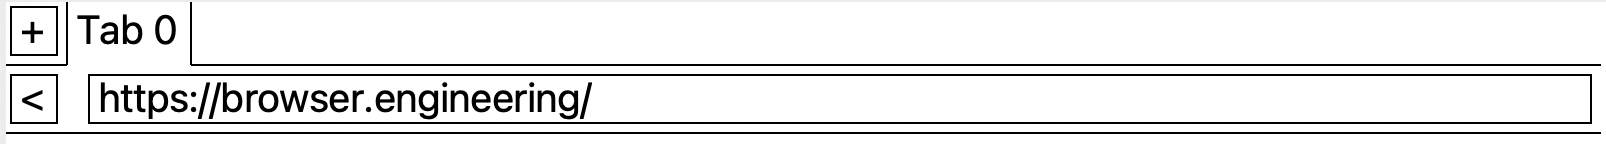
\includegraphics[width=0.9\textwidth]{im/chrome-chrome.png}
\caption{The intended appearance of the browser chrome.}\label{fig:BrowserChrome}
\end{figure}

% \end{center}

A lot of this design involves text, so let's start by picking a font:
\begin{Shaded}
\begin{Highlighting}[]
\KeywordTok{class}\NormalTok{ Chrome:}
    \KeywordTok{def} \FunctionTok{\_\_init\_\_}\NormalTok{(}\VariableTok{self}\NormalTok{, browser):}
        \CommentTok{\# ...}
        \VariableTok{self}\NormalTok{.font }\OperatorTok{=}\NormalTok{ get\_font(}\DecValTok{20}\NormalTok{, }\StringTok{"normal"}\NormalTok{, }\StringTok{"roman"}\NormalTok{)}
        \VariableTok{self}\NormalTok{.font\_height }\OperatorTok{=} \VariableTok{self}\NormalTok{.font.metrics(}\StringTok{"linespace"}\NormalTok{)}
\end{Highlighting}
\end{Shaded}
Because different operating systems draw fonts differently, we'll need
to adjust the exact design of the browser chrome based on font metrics.
So we'll need the \texttt{font\_height} later.\footnote{I chose
  \texttt{20px} as the font size, but that might be too large on your
  device\index{device
  pixel ratio}. Feel free to adjust.}

Using that font height, we can now determine where the tab bar starts
and ends:
\begin{Shaded}
\begin{Highlighting}[]
\KeywordTok{class}\NormalTok{ Chrome:}
    \KeywordTok{def} \FunctionTok{\_\_init\_\_}\NormalTok{(}\VariableTok{self}\NormalTok{, browser):}
        \CommentTok{\# ...}
        \VariableTok{self}\NormalTok{.padding }\OperatorTok{=} \DecValTok{5}
        \VariableTok{self}\NormalTok{.tabbar\_top }\OperatorTok{=} \DecValTok{0}
        \VariableTok{self}\NormalTok{.tabbar\_bottom }\OperatorTok{=} \VariableTok{self}\NormalTok{.font\_height }\OperatorTok{+} \DecValTok{2}\OperatorTok{*}\VariableTok{self}\NormalTok{.padding}
\end{Highlighting}
\end{Shaded}
Note that I've added some padding so that text doesn't run into the edge
of the window.

We will store rectangles representing the size of various elements in
the browser chrome. For that, a new \texttt{Rect} class will be
convenient:
\begin{Shaded}
\begin{Highlighting}[]
\KeywordTok{class}\NormalTok{ Rect:}
    \KeywordTok{def} \FunctionTok{\_\_init\_\_}\NormalTok{(}\VariableTok{self}\NormalTok{, left, top, right, bottom):}
        \VariableTok{self}\NormalTok{.left }\OperatorTok{=}\NormalTok{ left}
        \VariableTok{self}\NormalTok{.top }\OperatorTok{=}\NormalTok{ top}
        \VariableTok{self}\NormalTok{.right }\OperatorTok{=}\NormalTok{ right}
        \VariableTok{self}\NormalTok{.bottom }\OperatorTok{=}\NormalTok{ bottom}
\end{Highlighting}
\end{Shaded}

Now, this tab row needs to contain a new-tab button and the tab names
themselves.
I'll add padding around the new-tab button:
\begin{Shaded}
\begin{Highlighting}[]
\KeywordTok{class}\NormalTok{ Chrome:}
    \KeywordTok{def} \FunctionTok{\_\_init\_\_}\NormalTok{(}\VariableTok{self}\NormalTok{, browser):}
        \CommentTok{\# ...}
\NormalTok{        plus\_width }\OperatorTok{=} \VariableTok{self}\NormalTok{.font.measure(}\StringTok{"+"}\NormalTok{) }\OperatorTok{+} \DecValTok{2}\OperatorTok{*}\VariableTok{self}\NormalTok{.padding}
        \VariableTok{self}\NormalTok{.newtab\_rect }\OperatorTok{=}\NormalTok{ Rect(}
           \VariableTok{self}\NormalTok{.padding, }\VariableTok{self}\NormalTok{.padding,}
           \VariableTok{self}\NormalTok{.padding }\OperatorTok{+}\NormalTok{ plus\_width,}
           \VariableTok{self}\NormalTok{.padding }\OperatorTok{+} \VariableTok{self}\NormalTok{.font\_height)}
\end{Highlighting}
\end{Shaded}
Then the tabs will start \texttt{padding} past the end of the new-tab
button. Because the number of tabs can change, I'm not going to store
the location of each tab. Instead, I'll just compute their bounds on the
fly:
\begin{Shaded}
\begin{Highlighting}[]
\KeywordTok{class}\NormalTok{ Chrome:}
    \KeywordTok{def}\NormalTok{ tab\_rect(}\VariableTok{self}\NormalTok{, i):}
\NormalTok{        tabs\_start }\OperatorTok{=} \VariableTok{self}\NormalTok{.newtab\_rect.right }\OperatorTok{+} \VariableTok{self}\NormalTok{.padding}
\NormalTok{        tab\_width }\OperatorTok{=} \VariableTok{self}\NormalTok{.font.measure(}\StringTok{"Tab X"}\NormalTok{) }\OperatorTok{+} \DecValTok{2}\OperatorTok{*}\VariableTok{self}\NormalTok{.padding}
        \ControlFlowTok{return}\NormalTok{ Rect(}
\NormalTok{            tabs\_start }\OperatorTok{+}\NormalTok{ tab\_width }\OperatorTok{*}\NormalTok{ i, }\VariableTok{self}\NormalTok{.tabbar\_top,}
\NormalTok{            tabs\_start }\OperatorTok{+}\NormalTok{ tab\_width }\OperatorTok{*}\NormalTok{ (i }\OperatorTok{+} \DecValTok{1}\NormalTok{), }\VariableTok{self}\NormalTok{.tabbar\_bottom)}
\end{Highlighting}
\end{Shaded}
Note that I measure the text ``Tab X'' and use that for all of the tab
widths. This is not quite right---in many fonts, numbers like~8 are
wider than numbers like~1---but it is close enough, and anyway, the
letter X is typically as wide as the widest number.

To actually draw the UI, we'll first have the browser chrome paint a
display list, which the \texttt{Browser} will then draw to the screen:

\begin{Shaded}
\begin{Highlighting}[]
\KeywordTok{class}\NormalTok{ Chrome:}
    \KeywordTok{def}\NormalTok{ paint(}\VariableTok{self}\NormalTok{):}
\NormalTok{        cmds }\OperatorTok{=}\NormalTok{ []}
        \CommentTok{\# ...}
        \ControlFlowTok{return}\NormalTok{ cmds}
\end{Highlighting}
\end{Shaded}

Let's start by first painting the new-tab button:
\begin{Shaded}
\begin{Highlighting}[]
\KeywordTok{class}\NormalTok{ Chrome:}
    \KeywordTok{def}\NormalTok{ paint(}\VariableTok{self}\NormalTok{):}
        \CommentTok{\# ...}
\NormalTok{        cmds.append(DrawOutline(}\VariableTok{self}\NormalTok{.newtab\_rect, }\StringTok{"black"}\NormalTok{, }\DecValTok{1}\NormalTok{))}
\NormalTok{        cmds.append(DrawText(}
            \VariableTok{self}\NormalTok{.newtab\_rect.left }\OperatorTok{+} \VariableTok{self}\NormalTok{.padding,}
            \VariableTok{self}\NormalTok{.newtab\_rect.top,}
            \StringTok{"+"}\NormalTok{, }\VariableTok{self}\NormalTok{.font, }\StringTok{"black"}\NormalTok{))}
\end{Highlighting}
\end{Shaded}
The \texttt{DrawOutline} command draws a rectangular border:
\begin{Shaded}
\begin{Highlighting}[]
\KeywordTok{class}\NormalTok{ DrawOutline:}
    \KeywordTok{def} \FunctionTok{\_\_init\_\_}\NormalTok{(}\VariableTok{self}\NormalTok{, rect, color, thickness):}
        \VariableTok{self}\NormalTok{.rect }\OperatorTok{=}\NormalTok{ rect}
        \VariableTok{self}\NormalTok{.color }\OperatorTok{=}\NormalTok{ color}
        \VariableTok{self}\NormalTok{.thickness }\OperatorTok{=}\NormalTok{ thickness}

    \KeywordTok{def}\NormalTok{ execute(}\VariableTok{self}\NormalTok{, scroll, canvas):}
\NormalTok{        canvas.create\_rectangle(}
            \VariableTok{self}\NormalTok{.rect.left, }\VariableTok{self}\NormalTok{.rect.top }\OperatorTok{{-}}\NormalTok{ scroll,}
            \VariableTok{self}\NormalTok{.rect.right, }\VariableTok{self}\NormalTok{.rect.bottom }\OperatorTok{{-}}\NormalTok{ scroll,}
\NormalTok{            width}\OperatorTok{=}\VariableTok{self}\NormalTok{.thickness,}
\NormalTok{            outline}\OperatorTok{=}\VariableTok{self}\NormalTok{.color)}
\end{Highlighting}
\end{Shaded}

Next up is drawing the tabs. Python's \texttt{enumerate} function lets
you iterate over both the indices and the contents of an array at the
same time. For each tab, we need to create a border on the left and
right and then draw the tab name:
\begin{Shaded}
\begin{Highlighting}[]
\KeywordTok{class}\NormalTok{ Chrome:}
    \KeywordTok{def}\NormalTok{ paint(}\VariableTok{self}\NormalTok{):}
        \CommentTok{\# ...}
        \ControlFlowTok{for}\NormalTok{ i, tab }\KeywordTok{in} \BuiltInTok{enumerate}\NormalTok{(}\VariableTok{self}\NormalTok{.browser.tabs):}
\NormalTok{            bounds }\OperatorTok{=} \VariableTok{self}\NormalTok{.tab\_rect(i)}
\NormalTok{            cmds.append(DrawLine(}
\NormalTok{                bounds.left, }\DecValTok{0}\NormalTok{, bounds.left, bounds.bottom,}
                \StringTok{"black"}\NormalTok{, }\DecValTok{1}\NormalTok{))}
\NormalTok{            cmds.append(DrawLine(}
\NormalTok{                bounds.right, }\DecValTok{0}\NormalTok{, bounds.right, bounds.bottom,}
                \StringTok{"black"}\NormalTok{, }\DecValTok{1}\NormalTok{))}
\NormalTok{            cmds.append(DrawText(}
\NormalTok{                bounds.left }\OperatorTok{+} \VariableTok{self}\NormalTok{.padding, bounds.top }\OperatorTok{+} \VariableTok{self}\NormalTok{.padding,}
                \StringTok{"Tab }\SpecialCharTok{\{\}}\StringTok{"}\NormalTok{.}\BuiltInTok{format}\NormalTok{(i), }\VariableTok{self}\NormalTok{.font, }\StringTok{"black"}\NormalTok{))}
\end{Highlighting}
\end{Shaded}

Finally, to identify which tab is the active tab, we've got to make that
file folder shape with the current tab sticking up:
\begin{Shaded}
\begin{Highlighting}[]
\KeywordTok{class}\NormalTok{ Chrome:}
    \KeywordTok{def}\NormalTok{ paint(}\VariableTok{self}\NormalTok{):}
        \ControlFlowTok{for}\NormalTok{ i, tab }\KeywordTok{in} \BuiltInTok{enumerate}\NormalTok{(}\VariableTok{self}\NormalTok{.browser.tabs):}
            \CommentTok{\# ...}
            \ControlFlowTok{if}\NormalTok{ tab }\OperatorTok{==} \VariableTok{self}\NormalTok{.browser.active\_tab:}
\NormalTok{                cmds.append(DrawLine(}
                    \DecValTok{0}\NormalTok{, bounds.bottom, bounds.left, bounds.bottom,}
                    \StringTok{"black"}\NormalTok{, }\DecValTok{1}\NormalTok{))}
\NormalTok{                cmds.append(DrawLine(}
\NormalTok{                    bounds.right, bounds.bottom, WIDTH, bounds.bottom,}
                    \StringTok{"black"}\NormalTok{, }\DecValTok{1}\NormalTok{))}
\end{Highlighting}
\end{Shaded}
The \texttt{DrawLine} command draws a line of a given color and
thickness. It's defined like so:
\begin{Shaded}
\begin{Highlighting}[]
\KeywordTok{class}\NormalTok{ DrawLine:}
    \KeywordTok{def} \FunctionTok{\_\_init\_\_}\NormalTok{(}\VariableTok{self}\NormalTok{, x1, y1, x2, y2, color, thickness):}
        \VariableTok{self}\NormalTok{.rect }\OperatorTok{=}\NormalTok{ Rect(x1, y1, x2, y2)}
        \VariableTok{self}\NormalTok{.color }\OperatorTok{=}\NormalTok{ color}
        \VariableTok{self}\NormalTok{.thickness }\OperatorTok{=}\NormalTok{ thickness}

    \KeywordTok{def}\NormalTok{ execute(}\VariableTok{self}\NormalTok{, scroll, canvas):}
\NormalTok{        canvas.create\_line(}
            \VariableTok{self}\NormalTok{.rect.left, }\VariableTok{self}\NormalTok{.rect.top }\OperatorTok{{-}}\NormalTok{ scroll,}
            \VariableTok{self}\NormalTok{.rect.right, }\VariableTok{self}\NormalTok{.rect.bottom }\OperatorTok{{-}}\NormalTok{ scroll,}
\NormalTok{            fill}\OperatorTok{=}\VariableTok{self}\NormalTok{.color, width}\OperatorTok{=}\VariableTok{self}\NormalTok{.thickness)}
\end{Highlighting}
\end{Shaded}

One final thing: we want to make sure that the browser chrome is always
drawn on top of the page contents. To guarantee that, we can draw a
white rectangle behind the chrome:
\begin{Shaded}
\begin{Highlighting}[]
\KeywordTok{class}\NormalTok{ Chrome:}
    \KeywordTok{def} \FunctionTok{\_\_init\_\_}\NormalTok{(}\VariableTok{self}\NormalTok{, browser):}
        \CommentTok{\# ...}
        \VariableTok{self}\NormalTok{.bottom }\OperatorTok{=} \VariableTok{self}\NormalTok{.tabbar\_bottom}

    \KeywordTok{def}\NormalTok{ paint(}\VariableTok{self}\NormalTok{):}
        \CommentTok{\# ...}
\NormalTok{        cmds.append(DrawRect(}
\NormalTok{            Rect(}\DecValTok{0}\NormalTok{, }\DecValTok{0}\NormalTok{, WIDTH, }\VariableTok{self}\NormalTok{.bottom),}
            \StringTok{"white"}\NormalTok{))}
\NormalTok{        cmds.append(DrawLine(}
            \DecValTok{0}\NormalTok{, }\VariableTok{self}\NormalTok{.bottom, WIDTH,}
            \VariableTok{self}\NormalTok{.bottom, }\StringTok{"black"}\NormalTok{, }\DecValTok{1}\NormalTok{))}
        \CommentTok{\# ...}
\end{Highlighting}
\end{Shaded}
Make sure the background is drawn before any other part of the chrome.
I also added a line at the bottom of the chrome to separate it from the
page. Note how I also changed \texttt{DrawRect} to pass a \texttt{Rect}
instead of the four corners; this requires a change to
\texttt{BlockLayout}:
\begin{Shaded}
\begin{Highlighting}[]
\KeywordTok{class}\NormalTok{ BlockLayout:}
    \KeywordTok{def}\NormalTok{ self\_rect(}\VariableTok{self}\NormalTok{):}
        \ControlFlowTok{return}\NormalTok{ Rect(}\VariableTok{self}\NormalTok{.x, }\VariableTok{self}\NormalTok{.y,}
            \VariableTok{self}\NormalTok{.x }\OperatorTok{+} \VariableTok{self}\NormalTok{.width, }\VariableTok{self}\NormalTok{.y }\OperatorTok{+} \VariableTok{self}\NormalTok{.height)}

    \KeywordTok{def}\NormalTok{ paint(}\VariableTok{self}\NormalTok{):}
        \CommentTok{\# ...}
        \ControlFlowTok{if}\NormalTok{ bgcolor }\OperatorTok{!=} \StringTok{"transparent"}\NormalTok{:}
\NormalTok{            rect }\OperatorTok{=}\NormalTok{ DrawRect(}\VariableTok{self}\NormalTok{.self\_rect(), bgcolor)}
\NormalTok{            cmds.append(rect)}
        \ControlFlowTok{return}\NormalTok{ cmds}
\end{Highlighting}
\end{Shaded}
Add a \texttt{rect} field to \texttt{DrawText} and \texttt{DrawLine}
too.

Drawing this chrome display list is now straightforward:
\begin{Shaded}
\begin{Highlighting}[]
\KeywordTok{class}\NormalTok{ Browser:}
    \KeywordTok{def}\NormalTok{ draw(}\VariableTok{self}\NormalTok{):}
        \CommentTok{\# ...}
        \ControlFlowTok{for}\NormalTok{ cmd }\KeywordTok{in} \VariableTok{self}\NormalTok{.chrome.paint():}
\NormalTok{            cmd.execute(}\DecValTok{0}\NormalTok{, }\VariableTok{self}\NormalTok{.canvas)}
\end{Highlighting}
\end{Shaded}
Note that this display list is always drawn at the top of the window,
unlike the tab contents (which scroll). Make sure to draw the chrome
\emph{after} the main tab contents, so that the chrome ends up on top.

However, we also have to make some adjustments to tab drawing to account
for the fact that the browser chrome takes up some vertical space. Let's
add a \texttt{tab\_height} parameter to \texttt{Tab}s:
\begin{Shaded}
\begin{Highlighting}[]
\KeywordTok{class}\NormalTok{ Tab:}
    \KeywordTok{def} \FunctionTok{\_\_init\_\_}\NormalTok{(}\VariableTok{self}\NormalTok{, tab\_height):}
        \CommentTok{\# ...}
        \VariableTok{self}\NormalTok{.tab\_height }\OperatorTok{=}\NormalTok{ tab\_height}
\end{Highlighting}
\end{Shaded}
We can pass it to \texttt{new\_tab}:
\begin{Shaded}
\begin{Highlighting}[]
\KeywordTok{class}\NormalTok{ Browser:}
    \KeywordTok{def}\NormalTok{ new\_tab(}\VariableTok{self}\NormalTok{, url):}
\NormalTok{        new\_tab }\OperatorTok{=}\NormalTok{ Tab(HEIGHT }\OperatorTok{{-}} \VariableTok{self}\NormalTok{.chrome.bottom)}
        \CommentTok{\# ...}
\end{Highlighting}
\end{Shaded}
We can then adjust \texttt{scrolldown} to account for the height of the
page content now being \texttt{tab\_height}:
\begin{Shaded}
\begin{Highlighting}[]
\KeywordTok{class}\NormalTok{ Tab:}
    \KeywordTok{def}\NormalTok{ scrolldown(}\VariableTok{self}\NormalTok{):}
\NormalTok{        max\_y }\OperatorTok{=} \BuiltInTok{max}\NormalTok{(}
            \VariableTok{self}\NormalTok{.document.height }\OperatorTok{+} \DecValTok{2}\OperatorTok{*}\NormalTok{VSTEP }\OperatorTok{{-}} \VariableTok{self}\NormalTok{.tab\_height, }\DecValTok{0}\NormalTok{)}
        \VariableTok{self}\NormalTok{.scroll }\OperatorTok{=} \BuiltInTok{min}\NormalTok{(}\VariableTok{self}\NormalTok{.scroll }\OperatorTok{+}\NormalTok{ SCROLL\_STEP, max\_y)}
\end{Highlighting}
\end{Shaded}

Finally, in \texttt{Tab}'s \texttt{draw} method we need to shift the
drawing commands down by the chrome height. I'll pass the chrome height
in as an \texttt{offset} parameter:
\begin{Shaded}
\begin{Highlighting}[]
\KeywordTok{class}\NormalTok{ Tab:}
    \KeywordTok{def}\NormalTok{ draw(}\VariableTok{self}\NormalTok{, canvas, offset):}
        \ControlFlowTok{for}\NormalTok{ cmd }\KeywordTok{in} \VariableTok{self}\NormalTok{.display\_list:}
            \ControlFlowTok{if}\NormalTok{ cmd.rect.top }\OperatorTok{\textgreater{}} \VariableTok{self}\NormalTok{.scroll }\OperatorTok{+} \VariableTok{self}\NormalTok{.tab\_height:}
                \ControlFlowTok{continue}
            \ControlFlowTok{if}\NormalTok{ cmd.rect.bottom }\OperatorTok{\textless{}} \VariableTok{self}\NormalTok{.scroll: }\ControlFlowTok{continue}
\NormalTok{            cmd.execute(}\VariableTok{self}\NormalTok{.scroll }\OperatorTok{{-}}\NormalTok{ offset, canvas)}
\end{Highlighting}
\end{Shaded}
The \texttt{Browser}'s final \texttt{draw} method now looks like this:
\begin{Shaded}
\begin{Highlighting}[]
\KeywordTok{class}\NormalTok{ Browser:}
    \KeywordTok{def}\NormalTok{ draw(}\VariableTok{self}\NormalTok{):}
        \VariableTok{self}\NormalTok{.canvas.delete(}\StringTok{"all"}\NormalTok{)}
        \VariableTok{self}\NormalTok{.active\_tab.draw(}\VariableTok{self}\NormalTok{.canvas, }\VariableTok{self}\NormalTok{.chrome.bottom)}
        \ControlFlowTok{for}\NormalTok{ cmd }\KeywordTok{in} \VariableTok{self}\NormalTok{.chrome.paint():}
\NormalTok{            cmd.execute(}\DecValTok{0}\NormalTok{, }\VariableTok{self}\NormalTok{.canvas)}
\end{Highlighting}
\end{Shaded}

One more thing: clicking on tabs to switch between them. The
\texttt{Browser} handles the click and now needs to delegate clicks on
the browser chrome to the \texttt{Chrome} object:
\begin{Shaded}
\begin{Highlighting}[]
\KeywordTok{class}\NormalTok{ Browser:}
    \KeywordTok{def}\NormalTok{ handle\_click(}\VariableTok{self}\NormalTok{, e):}
        \ControlFlowTok{if}\NormalTok{ e.y }\OperatorTok{\textless{}} \VariableTok{self}\NormalTok{.chrome.bottom:}
            \VariableTok{self}\NormalTok{.chrome.click(e.x, e.y)}
        \ControlFlowTok{else}\NormalTok{:}
\NormalTok{            tab\_y }\OperatorTok{=}\NormalTok{ e.y }\OperatorTok{{-}} \VariableTok{self}\NormalTok{.chrome.bottom}
            \VariableTok{self}\NormalTok{.active\_tab.click(e.x, tab\_y)}
        \VariableTok{self}\NormalTok{.draw()}
\end{Highlighting}
\end{Shaded}
Note that we need to subtract out the chrome size when clicking on
tab contents. As for clicks on the browser chrome, inside
\texttt{Chrome} we need to figure out what the user clicked on. To make
that easier, let's add a quick method to test whether a point is
contained in a \texttt{Rect}:
\begin{Shaded}
\begin{Highlighting}[]
\KeywordTok{class}\NormalTok{ Rect:}
    \KeywordTok{def}\NormalTok{ containsPoint(}\VariableTok{self}\NormalTok{, x, y):}
        \ControlFlowTok{return}\NormalTok{ x }\OperatorTok{\textgreater{}=} \VariableTok{self}\NormalTok{.left }\KeywordTok{and}\NormalTok{ x }\OperatorTok{\textless{}} \VariableTok{self}\NormalTok{.right }\OperatorTok{\textbackslash{}}
            \KeywordTok{and}\NormalTok{ y }\OperatorTok{\textgreater{}=} \VariableTok{self}\NormalTok{.top }\KeywordTok{and}\NormalTok{ y }\OperatorTok{\textless{}} \VariableTok{self}\NormalTok{.bottom}
\end{Highlighting}
\end{Shaded}
We use this method to handle clicks inside \texttt{Chrome},
and then use it to choose between clicking to add a tab or select an
open tab.
\begin{Shaded}
\begin{Highlighting}[]
\KeywordTok{class}\NormalTok{ Chrome:}
    \KeywordTok{def}\NormalTok{ click(}\VariableTok{self}\NormalTok{, x, y):}
        \ControlFlowTok{if} \VariableTok{self}\NormalTok{.newtab\_rect.containsPoint(x, y):}
            \VariableTok{self}\NormalTok{.browser.new\_tab(URL(}\StringTok{"https://browser.engineering/"}\NormalTok{))}
        \ControlFlowTok{else}\NormalTok{:}
            \ControlFlowTok{for}\NormalTok{ i, tab }\KeywordTok{in} \BuiltInTok{enumerate}\NormalTok{(}\VariableTok{self}\NormalTok{.browser.tabs):}
                \ControlFlowTok{if} \VariableTok{self}\NormalTok{.tab\_rect(i).containsPoint(x, y):}
                    \VariableTok{self}\NormalTok{.browser.active\_tab }\OperatorTok{=}\NormalTok{ tab}
                    \ControlFlowTok{break}
\end{Highlighting}
\end{Shaded}
That's an appropriate ``new tab'' page, don't you think? Anyway, you
should now be able to load multiple tabs, scroll and click around them
independently, and switch tabs by clicking on them.

\begin{bookblock}{further}
Google Chrome 1.0 was accompanied by a
\href{https://www.google.com/googlebooks/chrome/}{comic book} to pitch
its features. There's a whole
\href{https://www.google.com/googlebooks/chrome/big_18.html}{chapter}
about its design ideas and user interface features, many of which stuck
around. Even this book's browser has tabs on top, for example.
\end{bookblock}

\hypertarget{navigation-history}{%
\section{Navigation History}\label{navigation-history}}

Now that we are navigating between pages all the time, it's easy to get
a little lost and forget what web page you're looking at. An address bar
that shows the current URL would help a lot. Let's make room for it in
the chrome:
\begin{Shaded}
\begin{Highlighting}[]
\KeywordTok{class}\NormalTok{ Chrome:}
    \KeywordTok{def} \FunctionTok{\_\_init\_\_}\NormalTok{(}\VariableTok{self}\NormalTok{, browser):}
        \CommentTok{\# ...}
        \VariableTok{self}\NormalTok{.urlbar\_top }\OperatorTok{=} \VariableTok{self}\NormalTok{.tabbar\_bottom}
        \VariableTok{self}\NormalTok{.urlbar\_bottom }\OperatorTok{=} \VariableTok{self}\NormalTok{.urlbar\_top }\OperatorTok{+} \OperatorTok{\textbackslash{}}
            \VariableTok{self}\NormalTok{.font\_height }\OperatorTok{+} \DecValTok{2}\OperatorTok{*}\VariableTok{self}\NormalTok{.padding}
        \VariableTok{self}\NormalTok{.bottom }\OperatorTok{=} \VariableTok{self}\NormalTok{.urlbar\_bottom}
\end{Highlighting}
\end{Shaded}

This ``URL bar'' will contain the back button and the address bar:
\begin{Shaded}
\begin{Highlighting}[]
\KeywordTok{class}\NormalTok{ Chrome:}
    \KeywordTok{def} \FunctionTok{\_\_init\_\_}\NormalTok{(}\VariableTok{self}\NormalTok{, browser):}
        \CommentTok{\# ...}
\NormalTok{        back\_width }\OperatorTok{=} \VariableTok{self}\NormalTok{.font.measure(}\StringTok{"\textless{}"}\NormalTok{) }\OperatorTok{+} \DecValTok{2}\OperatorTok{*}\VariableTok{self}\NormalTok{.padding}
        \VariableTok{self}\NormalTok{.back\_rect }\OperatorTok{=}\NormalTok{ Rect(}
            \VariableTok{self}\NormalTok{.padding,}
            \VariableTok{self}\NormalTok{.urlbar\_top }\OperatorTok{+} \VariableTok{self}\NormalTok{.padding,}
            \VariableTok{self}\NormalTok{.padding }\OperatorTok{+}\NormalTok{ back\_width,}
            \VariableTok{self}\NormalTok{.urlbar\_bottom }\OperatorTok{{-}} \VariableTok{self}\NormalTok{.padding)}

        \VariableTok{self}\NormalTok{.address\_rect }\OperatorTok{=}\NormalTok{ Rect(}
            \VariableTok{self}\NormalTok{.back\_rect.top }\OperatorTok{+} \VariableTok{self}\NormalTok{.padding,}
            \VariableTok{self}\NormalTok{.urlbar\_top }\OperatorTok{+} \VariableTok{self}\NormalTok{.padding,}
\NormalTok{            WIDTH }\OperatorTok{{-}} \VariableTok{self}\NormalTok{.padding,}
            \VariableTok{self}\NormalTok{.urlbar\_bottom }\OperatorTok{{-}} \VariableTok{self}\NormalTok{.padding)}
\end{Highlighting}
\end{Shaded}
Painting the back button is straightforward:
\begin{Shaded}
\begin{Highlighting}[]
\KeywordTok{class}\NormalTok{ Chrome:}
    \KeywordTok{def}\NormalTok{ paint(}\VariableTok{self}\NormalTok{):}
        \CommentTok{\# ...}
\NormalTok{        cmds.append(DrawOutline(}\VariableTok{self}\NormalTok{.back\_rect, }\StringTok{"black"}\NormalTok{, }\DecValTok{1}\NormalTok{))}
\NormalTok{        cmds.append(DrawText(}
            \VariableTok{self}\NormalTok{.back\_rect.left }\OperatorTok{+} \VariableTok{self}\NormalTok{.padding,}
            \VariableTok{self}\NormalTok{.back\_rect.top,}
            \StringTok{"\textless{}"}\NormalTok{, }\VariableTok{self}\NormalTok{.font, }\StringTok{"black"}\NormalTok{))}
\end{Highlighting}
\end{Shaded}

The address bar needs to get the current tab's URL from the browser:
\begin{Shaded}
\begin{Highlighting}[]
\KeywordTok{class}\NormalTok{ Chrome:}
    \KeywordTok{def}\NormalTok{ paint(}\VariableTok{self}\NormalTok{):}
        \CommentTok{\# ...}
\NormalTok{        cmds.append(DrawOutline(}\VariableTok{self}\NormalTok{.address\_rect, }\StringTok{"black"}\NormalTok{, }\DecValTok{1}\NormalTok{))}
\NormalTok{        url }\OperatorTok{=} \BuiltInTok{str}\NormalTok{(}\VariableTok{self}\NormalTok{.browser.active\_tab.url)}
\NormalTok{            cmds.append(DrawText(}
                \VariableTok{self}\NormalTok{.address\_rect.left }\OperatorTok{+} \VariableTok{self}\NormalTok{.padding,}
                \VariableTok{self}\NormalTok{.address\_rect.top,}
\NormalTok{                url, }\VariableTok{self}\NormalTok{.font, }\StringTok{"black"}\NormalTok{))}
\end{Highlighting}
\end{Shaded}
Here, \texttt{str} is a built-in Python function that we can override to
correctly convert \texttt{URL} objects to strings:
\begin{Shaded}
\begin{Highlighting}[]
\KeywordTok{class}\NormalTok{ URL:}
    \KeywordTok{def} \FunctionTok{\_\_str\_\_}\NormalTok{(}\VariableTok{self}\NormalTok{):}
\NormalTok{        port\_part }\OperatorTok{=} \StringTok{":"} \OperatorTok{+} \BuiltInTok{str}\NormalTok{(}\VariableTok{self}\NormalTok{.port)}
        \ControlFlowTok{if} \VariableTok{self}\NormalTok{.scheme }\OperatorTok{==} \StringTok{"https"} \KeywordTok{and} \VariableTok{self}\NormalTok{.port }\OperatorTok{==} \DecValTok{443}\NormalTok{:}
\NormalTok{            port\_part }\OperatorTok{=} \StringTok{""}
        \ControlFlowTok{if} \VariableTok{self}\NormalTok{.scheme }\OperatorTok{==} \StringTok{"http"} \KeywordTok{and} \VariableTok{self}\NormalTok{.port }\OperatorTok{==} \DecValTok{80}\NormalTok{:}
\NormalTok{            port\_part }\OperatorTok{=} \StringTok{""}
        \ControlFlowTok{return} \VariableTok{self}\NormalTok{.scheme }\OperatorTok{+} \StringTok{"://"} \OperatorTok{+} \VariableTok{self}\NormalTok{.host }\OperatorTok{+}\NormalTok{ port\_part }\OperatorTok{+} \VariableTok{self}\NormalTok{.path}
\end{Highlighting}
\end{Shaded}
I think the extra logic to hide port numbers is worth it to make the
URLs more tidy.

What should happen when the back button is clicked? Well, \emph{that
tab} should go back. Other tabs are not affected. So the
\texttt{Browser} has to invoke some method on the current tab to go
back:
\begin{Shaded}
\begin{Highlighting}[]
\KeywordTok{class}\NormalTok{ Chrome:}
    \KeywordTok{def}\NormalTok{ click(}\VariableTok{self}\NormalTok{, x, y):}
        \CommentTok{\# ...}
        \ControlFlowTok{elif} \VariableTok{self}\NormalTok{.back\_rect.containsPoint(x, y):}
            \VariableTok{self}\NormalTok{.browser.active\_tab.go\_back()}
\end{Highlighting}
\end{Shaded}
For the active tab to ``go back'', it needs to store a ``history'' of
which pages it's visited before:
\begin{Shaded}
\begin{Highlighting}[]
\KeywordTok{class}\NormalTok{ Tab:}
    \KeywordTok{def} \FunctionTok{\_\_init\_\_}\NormalTok{(}\VariableTok{self}\NormalTok{, tab\_height):}
        \CommentTok{\# ...}
        \VariableTok{self}\NormalTok{.history }\OperatorTok{=}\NormalTok{ []}
\end{Highlighting}
\end{Shaded}
The history grows every time we go to a new page:
\begin{Shaded}
\begin{Highlighting}[]
\KeywordTok{class}\NormalTok{ Tab:}
    \KeywordTok{def}\NormalTok{ load(}\VariableTok{self}\NormalTok{, url):}
        \VariableTok{self}\NormalTok{.history.append(url)}
        \CommentTok{\# ...}
\end{Highlighting}
\end{Shaded}
Going back uses that history. You might think to write this:
\begin{Shaded}
\begin{Highlighting}[]
\KeywordTok{class}\NormalTok{ Tab:}
    \KeywordTok{def}\NormalTok{ go\_back(}\VariableTok{self}\NormalTok{):}
        \ControlFlowTok{if} \BuiltInTok{len}\NormalTok{(}\VariableTok{self}\NormalTok{.history) }\OperatorTok{\textgreater{}} \DecValTok{1}\NormalTok{:}
            \VariableTok{self}\NormalTok{.load(}\VariableTok{self}\NormalTok{.history[}\OperatorTok{{-}}\DecValTok{2}\NormalTok{])}
\end{Highlighting}
\end{Shaded}
That's almost correct, but it doesn't work if you click the back button
twice, because \texttt{load} adds to the history. Instead, we need to do
something more like this:
\begin{Shaded}
\begin{Highlighting}[]
\KeywordTok{class}\NormalTok{ Tab:}
    \KeywordTok{def}\NormalTok{ go\_back(}\VariableTok{self}\NormalTok{):}
        \ControlFlowTok{if} \BuiltInTok{len}\NormalTok{(}\VariableTok{self}\NormalTok{.history) }\OperatorTok{\textgreater{}} \DecValTok{1}\NormalTok{:}
            \VariableTok{self}\NormalTok{.history.pop()}
\NormalTok{            back }\OperatorTok{=} \VariableTok{self}\NormalTok{.history.pop()}
            \VariableTok{self}\NormalTok{.load(back)}
\end{Highlighting}
\end{Shaded}
Now, going back shrinks the history and clicking on links grows it, as
it should.

So we've now got a pretty good web browser for reading this very book:
you can click links, browse around, and even have multiple chapters open
simultaneously for cross-referencing things. But it's a little hard to
visit a website not linked to from the current one.

\begin{bookblock}{further}
A browser's navigation history can contain sensitive information about
which websites a user likes visiting, so keeping it secure is important.
Surprisingly, this is pretty hard, because CSS features like the
\href{https://developer.mozilla.org/en-US/docs/Web/CSS/:visited}{\texttt{:visited}
selector} can be used to
\href{https://blog.mozilla.org/security/2010/03/31/plugging-the-css-history-leak/}{check}
whether a URL has been visited before. For this reason, there are
\href{https://github.com/kyraseevers/Partitioning-visited-links-history}{efforts}
to restrict \texttt{:visited}.
\end{bookblock}

\hypertarget{editing-the-url}{%
\section{Editing the URL}\label{editing-the-url}}

One way to go to another page is by clicking on a link. But most
browsers also allow you to type into the address bar to visit a new URL,
if you happen to know the URL. % off-hand.

Take a moment to notice the complex ritual of typing in an address (see Figure~\ref{fig:AddressBar}):
\begin{itemize}
%\tightlist
\item
  First, you have to click on the address bar to ``focus''\index{focus}
  on it.
\item
  That also selects the full address, so that it's all deleted when you
  start typing.
\item
  Then, letters you type go into the address bar.
\item
  The address bar updates as you type, but the browser doesn't yet
  navigate to the new page.
\item
  Finally, you type the ``Enter'' key which navigates to a new page.
\end{itemize}
% \begin{center}
\begin{figure}[tbp]
\centering
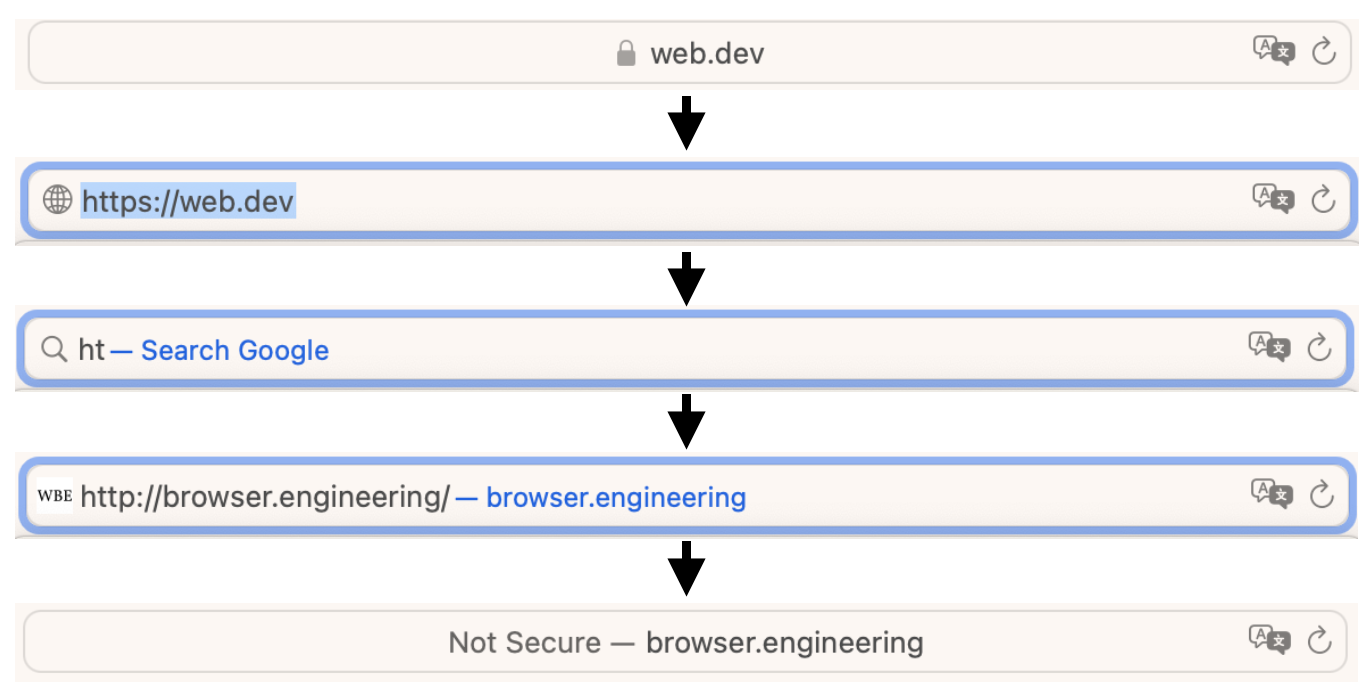
\includegraphics{im/chrome-editing.png}
\caption{Screenshots of editing in the address bar in Apple Safari 16.6.}\label{fig:AddressBar}
\end{figure}
%\end{center}
These steps suggest that the browser stores the contents of the address
bar separately from the \texttt{url} field, and also that there's some
state to say whether you're currently typing into the address bar. Let's
call the contents \texttt{address\_bar} and the state \texttt{focus}:
\begin{Shaded}
\begin{Highlighting}[]
\KeywordTok{class}\NormalTok{ Chrome:}
    \KeywordTok{def} \FunctionTok{\_\_init\_\_}\NormalTok{(}\VariableTok{self}\NormalTok{, browser):}
        \CommentTok{\# ...}
        \VariableTok{self}\NormalTok{.focus }\OperatorTok{=} \VariableTok{None}
        \VariableTok{self}\NormalTok{.address\_bar }\OperatorTok{=} \StringTok{""}
\end{Highlighting}
\end{Shaded}

Clicking on the address bar should set \texttt{focus} and clicking
outside it should clear \texttt{focus}:
\begin{Shaded}
\begin{Highlighting}[]
\KeywordTok{class}\NormalTok{ Chrome:}
    \KeywordTok{def}\NormalTok{ click(}\VariableTok{self}\NormalTok{, x, y):}
        \VariableTok{self}\NormalTok{.focus }\OperatorTok{=} \VariableTok{None}
        \CommentTok{\# ...}
        \ControlFlowTok{elif} \VariableTok{self}\NormalTok{.address\_rect.containsPoint(x, y):}
            \VariableTok{self}\NormalTok{.focus }\OperatorTok{=} \StringTok{"address bar"}
            \VariableTok{self}\NormalTok{.address\_bar }\OperatorTok{=} \StringTok{""}
\end{Highlighting}
\end{Shaded}
Note that clicking on the address bar also clears the address bar
contents. That's not quite what a browser does, but it's pretty close,
and lets us skip adding text selection.

Now, when we draw the address bar, we need to check whether to draw the
current URL or the currently typed text:
\begin{Shaded}
\begin{Highlighting}[]
\KeywordTok{class}\NormalTok{ Chrome:}
    \KeywordTok{def}\NormalTok{ paint(}\VariableTok{self}\NormalTok{):}
        \CommentTok{\# ...}
        \ControlFlowTok{if} \VariableTok{self}\NormalTok{.focus }\OperatorTok{==} \StringTok{"address bar"}\NormalTok{:}
\NormalTok{            cmds.append(DrawText(}
                \VariableTok{self}\NormalTok{.address\_rect.left }\OperatorTok{+} \VariableTok{self}\NormalTok{.padding,}
                \VariableTok{self}\NormalTok{.address\_rect.top,}
                \VariableTok{self}\NormalTok{.address\_bar, }\VariableTok{self}\NormalTok{.font, }\StringTok{"black"}\NormalTok{))}
        \ControlFlowTok{else}\NormalTok{:}
\NormalTok{            url }\OperatorTok{=} \BuiltInTok{str}\NormalTok{(}\VariableTok{self}\NormalTok{.browser.active\_tab.url)}
\NormalTok{            cmds.append(DrawText(}
                \VariableTok{self}\NormalTok{.address\_rect.left }\OperatorTok{+} \VariableTok{self}\NormalTok{.padding,}
                \VariableTok{self}\NormalTok{.address\_rect.top,}
\NormalTok{                url, }\VariableTok{self}\NormalTok{.font, }\StringTok{"black"}\NormalTok{))}
\end{Highlighting}
\end{Shaded}
When the user is typing in the address bar, let's also draw a cursor.
Making states (like focus) visible on the screen (like with the cursor)
makes software easier to use:
\begin{Shaded}
\begin{Highlighting}[]
\KeywordTok{class}\NormalTok{ Chrome:}
    \KeywordTok{def}\NormalTok{ paint(}\VariableTok{self}\NormalTok{):}
        \CommentTok{\# ...}
        \ControlFlowTok{if} \VariableTok{self}\NormalTok{.focus }\OperatorTok{==} \StringTok{"address bar"}\NormalTok{:}
            \CommentTok{\# ...}
\NormalTok{            w }\OperatorTok{=} \VariableTok{self}\NormalTok{.font.measure(}\VariableTok{self}\NormalTok{.address\_bar)}
\NormalTok{            cmds.append(DrawLine(}
                \VariableTok{self}\NormalTok{.address\_rect.left }\OperatorTok{+} \VariableTok{self}\NormalTok{.padding }\OperatorTok{+}\NormalTok{ w,}
                \VariableTok{self}\NormalTok{.address\_rect.top,}
                \VariableTok{self}\NormalTok{.address\_rect.left }\OperatorTok{+} \VariableTok{self}\NormalTok{.padding }\OperatorTok{+}\NormalTok{ w,}
                \VariableTok{self}\NormalTok{.address\_rect.bottom,}
                \StringTok{"red"}\NormalTok{, }\DecValTok{1}\NormalTok{))}
\end{Highlighting}
\end{Shaded}

Next, when the address bar is focused, we need to support typing in a
URL. In Tk, you can bind to \texttt{\textless{}Key\textgreater{}} to
capture all key presses. The event object's \texttt{char} field contains
the character the user typed.
\begin{Shaded}
\begin{Highlighting}[]
\KeywordTok{class}\NormalTok{ Browser:}
    \KeywordTok{def} \FunctionTok{\_\_init\_\_}\NormalTok{(}\VariableTok{self}\NormalTok{):}
        \CommentTok{\# ...}
        \VariableTok{self}\NormalTok{.window.bind(}\StringTok{"\textless{}Key\textgreater{}"}\NormalTok{, }\VariableTok{self}\NormalTok{.handle\_key)}

    \KeywordTok{def}\NormalTok{ handle\_key(}\VariableTok{self}\NormalTok{, e):}
        \ControlFlowTok{if} \BuiltInTok{len}\NormalTok{(e.char) }\OperatorTok{==} \DecValTok{0}\NormalTok{: }\ControlFlowTok{return}
        \ControlFlowTok{if} \KeywordTok{not}\NormalTok{ (}\BaseNTok{0x20} \OperatorTok{\textless{}=} \BuiltInTok{ord}\NormalTok{(e.char) }\OperatorTok{\textless{}} \BaseNTok{0x7f}\NormalTok{): }\ControlFlowTok{return}
        \VariableTok{self}\NormalTok{.chrome.keypress(e.char)}
        \VariableTok{self}\NormalTok{.draw()}
\end{Highlighting}
\end{Shaded}
This \texttt{handle\_key} handler starts with some conditions:
\texttt{\textless{}Key\textgreater{}} fires for every key press, not
just regular letters, so we want to ignore cases where no character is
typed (a modifier key is pressed) or the character is outside the ASCII
range (which can represent the arrow keys or function keys). For now
let's have the \texttt{Browser} send all key presses to \texttt{Chrome}
and then call \texttt{draw()} so that the new letters actually show up.
Then \texttt{Chrome} can check \texttt{focus} and add on to
\texttt{address\_bar}:
\begin{Shaded}
\begin{Highlighting}[]
\KeywordTok{class}\NormalTok{ Chrome:}
    \KeywordTok{def}\NormalTok{ keypress(}\VariableTok{self}\NormalTok{, char):}
        \ControlFlowTok{if} \VariableTok{self}\NormalTok{.focus }\OperatorTok{==} \StringTok{"address bar"}\NormalTok{:}
            \VariableTok{self}\NormalTok{.address\_bar }\OperatorTok{+=}\NormalTok{ char}
\end{Highlighting}
\end{Shaded}

Finally, once the new URL is entered, we need to handle the ``Enter''
key, which Tk calls \texttt{\textless{}Return\textgreater{}}, and
actually send the browser to the new address:
\begin{Shaded}
\begin{Highlighting}[]
\KeywordTok{class}\NormalTok{ Chrome:}
    \KeywordTok{def}\NormalTok{ enter(}\VariableTok{self}\NormalTok{):}
        \ControlFlowTok{if} \VariableTok{self}\NormalTok{.focus }\OperatorTok{==} \StringTok{"address bar"}\NormalTok{:}
            \VariableTok{self}\NormalTok{.browser.active\_tab.load(URL(}\VariableTok{self}\NormalTok{.address\_bar))}
            \VariableTok{self}\NormalTok{.focus }\OperatorTok{=} \VariableTok{None}

\KeywordTok{class}\NormalTok{ Browser:}
    \KeywordTok{def} \FunctionTok{\_\_init\_\_}\NormalTok{(}\VariableTok{self}\NormalTok{):}
        \CommentTok{\# ...}
        \VariableTok{self}\NormalTok{.window.bind(}\StringTok{"\textless{}Return\textgreater{}"}\NormalTok{, }\VariableTok{self}\NormalTok{.handle\_enter)}

    \KeywordTok{def}\NormalTok{ handle\_enter(}\VariableTok{self}\NormalTok{, e):}
        \VariableTok{self}\NormalTok{.chrome.enter()}
        \VariableTok{self}\NormalTok{.draw()}
\end{Highlighting}
\end{Shaded}

So there---after a long chapter, you can now unwind a bit by surfing the
web.

\begin{bookblock}{further}
Text editing is
\href{https://lord.io/text-editing-hates-you-too/}{surprisingly
complex}, and can be pretty tricky to implement well, especially for
languages other than English. And nowadays URLs can be written in
\href{https://en.wikipedia.org/wiki/Internationalized_domain_name}{any
language}, though modern browsers
\href{https://en.wikipedia.org/wiki/IDN_homograph_attack}{restrict this
somewhat} for security reasons.
\end{bookblock}

\hypertarget{summary}{%
\section{Summary}\label{ButtonsAndLinks-summary}}

It's been a lot of work just to handle links! We had to:
\begin{itemize}
% \tightlist
\item
  give each word an explicit size and position;
\item
  determine which piece of text a user clicked on;
\item
  split per-page from browser-wide information;
\item
  draw a tab bar, an address bar, and a back button;
\item
  even implement text editing!
\end{itemize}
Now just imagine all the features you can add to your browser!

\hypertarget{outline}{%
\section{Outline}\label{ButtonsAndLinks-outline}}

The complete set of functions, classes, and methods in our browser
should now look something like this:
\begin{Shaded}
\begin{Highlighting}[]
\NormalTok{WIDTH}
\NormalTok{HEIGHT}
\NormalTok{HSTEP}
\NormalTok{VSTEP}
\NormalTok{SCROLL\_STEP}
\NormalTok{FONTS}
\KeywordTok{def}\NormalTok{ get\_font(size, weight, slant)}
\KeywordTok{class}\NormalTok{ Text:}
    \KeywordTok{def} \FunctionTok{\_\_init\_\_}\NormalTok{(text, parent)}
    \KeywordTok{def} \FunctionTok{\_\_repr\_\_}\NormalTok{()}
\KeywordTok{class}\NormalTok{ Element:}
    \KeywordTok{def} \FunctionTok{\_\_init\_\_}\NormalTok{(tag, attributes, parent)}
    \KeywordTok{def} \FunctionTok{\_\_repr\_\_}\NormalTok{()}
\KeywordTok{def}\NormalTok{ print\_tree(node, indent)}
\KeywordTok{class}\NormalTok{ HTMLParser:}
    \KeywordTok{def} \FunctionTok{\_\_init\_\_}\NormalTok{(body)}
    \KeywordTok{def}\NormalTok{ parse()}
    \KeywordTok{def}\NormalTok{ get\_attributes(text)}
    \KeywordTok{def}\NormalTok{ add\_text(text)}
\NormalTok{    SELF\_CLOSING\_TAGS}
    \KeywordTok{def}\NormalTok{ add\_tag(tag)}
\NormalTok{    HEAD\_TAGS}
    \KeywordTok{def}\NormalTok{ implicit\_tags(tag)}
    \KeywordTok{def}\NormalTok{ finish()}
\NormalTok{BLOCK\_ELEMENTS}
\KeywordTok{class}\NormalTok{ DocumentLayout:}
    \KeywordTok{def} \FunctionTok{\_\_init\_\_}\NormalTok{(node)}
    \KeywordTok{def}\NormalTok{ layout()}
    \KeywordTok{def}\NormalTok{ paint()}
\KeywordTok{def}\NormalTok{ paint\_tree(layout\_object, display\_list)}
\KeywordTok{class}\NormalTok{ CSSParser:}
    \KeywordTok{def} \FunctionTok{\_\_init\_\_}\NormalTok{(s)}
    \KeywordTok{def}\NormalTok{ whitespace()}
    \KeywordTok{def}\NormalTok{ literal(literal)}
    \KeywordTok{def}\NormalTok{ word()}
    \KeywordTok{def}\NormalTok{ pair()}
    \KeywordTok{def}\NormalTok{ ignore\_until(chars)}
    \KeywordTok{def}\NormalTok{ body()}
    \KeywordTok{def}\NormalTok{ selector()}
    \KeywordTok{def}\NormalTok{ parse()}
\KeywordTok{class}\NormalTok{ TagSelector:}
    \KeywordTok{def} \FunctionTok{\_\_init\_\_}\NormalTok{(tag)}
    \KeywordTok{def}\NormalTok{ matches(node)}
\KeywordTok{class}\NormalTok{ DescendantSelector:}
    \KeywordTok{def} \FunctionTok{\_\_init\_\_}\NormalTok{(ancestor, descendant)}
    \KeywordTok{def}\NormalTok{ matches(node)}
\NormalTok{DEFAULT\_STYLE\_SHEET}
\NormalTok{INHERITED\_PROPERTIES}
\KeywordTok{def}\NormalTok{ style(node, rules)}
\KeywordTok{def}\NormalTok{ cascade\_priority(rule)}
\KeywordTok{class}\NormalTok{ DrawText:}
    \KeywordTok{def} \FunctionTok{\_\_init\_\_}\NormalTok{(x1, y1, text, font, color)}
    \KeywordTok{def}\NormalTok{ execute(scroll, canvas)}
\KeywordTok{class}\NormalTok{ URL:}
    \KeywordTok{def} \FunctionTok{\_\_init\_\_}\NormalTok{(url)}
    \KeywordTok{def}\NormalTok{ request()}
    \KeywordTok{def}\NormalTok{ resolve(url)}
    \KeywordTok{def} \FunctionTok{\_\_str\_\_}\NormalTok{()}
\KeywordTok{def}\NormalTok{ tree\_to\_list(tree, }\NormalTok{list}\NormalTok{)}
\KeywordTok{class}\NormalTok{ BlockLayout:}
    \KeywordTok{def} \FunctionTok{\_\_init\_\_}\NormalTok{(node, parent, previous)}
    \KeywordTok{def}\NormalTok{ token(tok)}
    \KeywordTok{def}\NormalTok{ word(node, word)}
    \KeywordTok{def}\NormalTok{ flush()}
    \KeywordTok{def}\NormalTok{ recurse(node)}
    \KeywordTok{def}\NormalTok{ layout()}
    \KeywordTok{def}\NormalTok{ layout\_mode()}
    \KeywordTok{def}\NormalTok{ paint()}
    \KeywordTok{def}\NormalTok{ new\_line()}
    \KeywordTok{def}\NormalTok{ self\_rect()}
\KeywordTok{class}\NormalTok{ LineLayout:}
    \KeywordTok{def} \FunctionTok{\_\_init\_\_}\NormalTok{(node, parent, previous)}
    \KeywordTok{def}\NormalTok{ layout()}
    \KeywordTok{def}\NormalTok{ paint()}
\KeywordTok{class}\NormalTok{ TextLayout:}
    \KeywordTok{def} \FunctionTok{\_\_init\_\_}\NormalTok{(node, word, parent, previous)}
    \KeywordTok{def}\NormalTok{ layout()}
    \KeywordTok{def}\NormalTok{ paint()}
\KeywordTok{class}\NormalTok{ DrawLine:}
    \KeywordTok{def} \FunctionTok{\_\_init\_\_}\NormalTok{(x1, y1, x2, y2, color, thickness)}
    \KeywordTok{def}\NormalTok{ execute(scroll, canvas)}
\KeywordTok{class}\NormalTok{ DrawOutline:}
    \KeywordTok{def} \FunctionTok{\_\_init\_\_}\NormalTok{(rect, color, thickness)}
    \KeywordTok{def}\NormalTok{ execute(scroll, canvas)}
\KeywordTok{class}\NormalTok{ Tab:}
    \KeywordTok{def} \FunctionTok{\_\_init\_\_}\NormalTok{(tab\_height)}
    \KeywordTok{def}\NormalTok{ load(url)}
    \KeywordTok{def}\NormalTok{ draw(canvas, offset)}
    \KeywordTok{def}\NormalTok{ scrolldown()}
    \KeywordTok{def}\NormalTok{ click(x, y)}
    \KeywordTok{def}\NormalTok{ go\_back()}
\KeywordTok{class}\NormalTok{ Rect:}
    \KeywordTok{def} \FunctionTok{\_\_init\_\_}\NormalTok{(left, top, right, bottom)}
    \KeywordTok{def}\NormalTok{ containsPoint(x, y)}
\KeywordTok{class}\NormalTok{ DrawRect:}
    \KeywordTok{def} \FunctionTok{\_\_init\_\_}\NormalTok{(rect, color)}
    \KeywordTok{def}\NormalTok{ execute(scroll, canvas)}
\KeywordTok{class}\NormalTok{ Chrome:}
    \KeywordTok{def} \FunctionTok{\_\_init\_\_}\NormalTok{(browser)}
    \KeywordTok{def}\NormalTok{ tab\_rect(i)}
    \KeywordTok{def}\NormalTok{ paint()}
    \KeywordTok{def}\NormalTok{ click(x, y)}
    \KeywordTok{def}\NormalTok{ keypress(char)}
    \KeywordTok{def}\NormalTok{ enter()}
\KeywordTok{class}\NormalTok{ Browser:}
    \KeywordTok{def} \FunctionTok{\_\_init\_\_}\NormalTok{()}
    \KeywordTok{def}\NormalTok{ handle\_down(e)}
    \KeywordTok{def}\NormalTok{ handle\_click(e)}
    \KeywordTok{def}\NormalTok{ handle\_key(e)}
    \KeywordTok{def}\NormalTok{ handle\_enter(e)}
    \KeywordTok{def}\NormalTok{ new\_tab(url)}
    \KeywordTok{def}\NormalTok{ draw()}
\end{Highlighting}
\end{Shaded}

\hypertarget{exercises}{%
\section{Exercises}\label{ButtonsAndLinks-exercises}}
\begin{enumerate}[label=\thechapter-\arabic*]
\item \emph{Backspace.} Add support for the backspace key when typing in the
address bar. Honestly, do this exercise just for your sanity.

\item \emph{Middle-click.} Add support for middle-clicking on a link
(\texttt{Button-2}) to open it in a new tab. You might want to use a
mouse when testing.

\item \emph{Window title.} Browsers set their window title to the contents of
the current tab's \texttt{\textless{}title\textgreater{}} element. Make
your browser do the same. You can call the \texttt{title} method of your
browser's \texttt{window} field to change the window title.

\item \emph{Forward.} Add a forward button, which should undo the back button.
If the most recent navigation action wasn't a back button, the forward
button shouldn't do anything.\footnote{To accomplish this, you'll need
  to keep around history items when clicking the back button, and store
  an index into it for the current page, instead of removing them
  entirely from the array.} Draw it in gray in that case, so the user
isn't stuck wondering why it doesn't work. Also draw the back button in
gray if there's nowhere to go back to.

\item \emph{Fragments.} URLs can contain a \emph{fragment}, which comes at the
end of a URL and is separated from the path by a hash sign \texttt{\#}.
When the browser navigates to a URL with a fragment, it should scroll
the page so that the element with that identifier is at the top of the
screen. Also, implement fragment links: relative URLs that begin with a
\texttt{\#} don't load a new page, but instead scroll the element with
that identifier to the top of the screen. The table of contents on
\href{https://browser.engineering/chrome.html}{the web version of this chapter} % page
uses fragment links.

\item \emph{Search.} If the user types something that's \emph{not} a URL into
the address bar, make your browser automatically search for it with a
search engine. This usually means going to a special URL. For example,
you can search Google by going to
\texttt{https://google.com/search?q=QUERY}, where \texttt{QUERY} is the
search query with every space replaced by a \texttt{+} sign.\footnote{Actually,
  you need to escape
  \href{https://en.wikipedia.org/wiki/Query_string\#URL_encoding}{lots
  of punctuation characters} in these ``query strings'', but that's kind
  of orthogonal to this address bar search feature.}

\item \emph{Visited links.} In real browsers, links you've visited before are
usually purple. Implement that feature. You'll need to store the set of
visited URLs, annotate the corresponding HTML elements, and check those
annotations when drawing the text.\footnote{Real browsers support
  special
  \href{https://developer.mozilla.org/en-US/docs/Web/CSS/Pseudo-classes}{pseudo-class}
  selectors that select all visited links, which you could implement if
  you want.}

\item \emph{Bookmarks.} Implement basic \emph{bookmarks}. Add a button to the
browser chrome; clicking it should bookmark the page. When you're
looking at a bookmarked page, that bookmark button should look different
(maybe yellow?) to remind the user that the page is bookmarked, and
clicking it should un-bookmark it. Add a special web page,
\texttt{about:bookmarks}, for viewing the list of bookmarks.

\item \emph{Cursor.} Make the left and right arrow keys move the text cursor
around the address bar when it is focused. Pressing the backspace key
should delete the character before the cursor, and typing other keys
should add characters at the cursor. (Remember that the cursor can be
before the first character or after the last!)

\item \emph{Multiple windows.} Add support for multiple browser windows in
addition to tabs. This will require keeping track of multiple Tk windows
and canvases and grouping tabs by their containing window. You'll also
need some way to create a new window, perhaps with a keypress such as
\texttt{Ctrl+N}.

\item\label{ex:DisplayList} \emph{Clicks via the display list.} At the moment, our browser converts
a click location to page coordinates and then finds the layout object at
those coordinates. But you could instead first look up the draw command
at that location, and then go from the draw command to the layout object
that generated it. Implement this. You'll need draw commands to know
which layout object generated them.\footnote{Real browsers don't
  currently do this, but it's an attractive possibility: display lists
  are pure data structures so access to them is easier to optimize or
  parallelize than the more complicated layout tree.}
\end{enumerate}

\ifprintedoutput
\theendnotes
\setcounter{endnote}{0}
\fi

\part{Running Applications}

\chapter{Sending Information to Servers}\label{ch:SendingInformation}
So far, our browser has seen the web as read only---but when you post on
Facebook, fill out a survey, or search Google, you're sending
information \emph{to} servers as well as receiving information
\emph{from} them. In this chapter, we'll start to transform our browser
into a platform for web applications by building out support for HTML
forms, the simplest way for a browser to send information to a server.

\hypertarget{how-forms-work}{%
\section{How Forms Work}\label{how-forms-work}}

HTML forms have a couple of moving parts.
First, in HTML there is a \texttt{form} element, which contains
\texttt{input} elements,\footnote{There are other elements similar to
  \texttt{input}, such as \texttt{select} and \texttt{textarea}. They
  work similarly enough; they just represent different kinds of user
  controls, like dropdowns and multi-line inputs.} which in turn can be
edited by the user. So a form might be written like this:
\begin{bookblock*}{notcode}
\begin{Shaded}
\begin{Highlighting}[]
\KeywordTok{\textless{}form} \ErrorTok{action}\OtherTok{=}\StringTok{"/submit"} \ErrorTok{method}\OtherTok{=}\StringTok{"post"}\KeywordTok{\textgreater{}}
    \KeywordTok{\textless{}p\textgreater{}}\NormalTok{Name: }\KeywordTok{\textless{}input} \ErrorTok{name}\OtherTok{=}\StringTok{name} \ErrorTok{value}\OtherTok{=}\StringTok{1}\KeywordTok{\textgreater{}\textless{}/p\textgreater{}}
    \KeywordTok{\textless{}p\textgreater{}}\NormalTok{Comment: }\KeywordTok{\textless{}input} \ErrorTok{name}\OtherTok{=}\StringTok{comment} \ErrorTok{value}\OtherTok{=}\StringTok{2}\KeywordTok{\textgreater{}\textless{}/p\textgreater{}}
    \KeywordTok{\textless{}p\textgreater{}\textless{}button\textgreater{}}\NormalTok{Submit!}\KeywordTok{\textless{}/button\textgreater{}\textless{}/p\textgreater{}}
\KeywordTok{\textless{}/form\textgreater{}}
\end{Highlighting}
\end{Shaded}
\end{bookblock*}
\noindent And look like Figure~\ref{fig:Form}. %this:

%\begin{center}

\begin{figure}
\centering
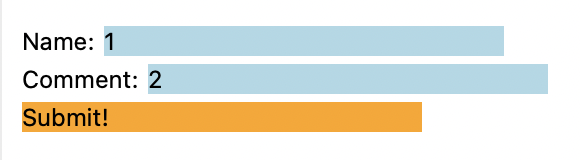
\includegraphics[width=0.8\textwidth]{im/forms-screenshot.png}
\caption{The example form in our browser.}\label{fig:Form}
\end{figure}

%\end{center}

This form contains two text entry boxes called \texttt{name} and
\texttt{comment}. When the user goes to this page, they can click on
those boxes to edit their values. Then, when they click the button at
the end of the form, the browser collects all of the name--value pairs
and bundles them into an HTTP \texttt{POST} request (as indicated by the
\texttt{method} attribute), sent to the URL given by the \texttt{form}
element's \texttt{action} attribute, with the usual rules of relative
URLs---so in this case, \texttt{/submit}. The \texttt{POST} request
looks like this:
\begin{bookblock*}{notcode}
\begin{Shaded}
\begin{Highlighting}[]
\NormalTok{POST /submit HTTP/1.0}
\NormalTok{Host: example.org}
\NormalTok{Content{-}Length: 16}

\NormalTok{name=1\&comment=2}
\end{Highlighting}
\end{Shaded}
\end{bookblock*}
\noindent In other words, it's a lot like the regular \texttt{GET} requests we've
already seen, except that it has a body---you've already seen HTTP
responses with bodies, but requests can have them too. Note the
\texttt{Content-Length} header; it's mandatory for \texttt{POST}
requests. The server responds to this request with a web page, just like
normal, and the browser then does everything it normally does.

Implementing forms requires extending many parts of the browser, from
implementing HTTP \texttt{POST} through new layout objects that draw
\texttt{input} elements to handling buttons clicks. That makes it a
great starting point for transforming our browser into an application
platform, our goal for the next few chapters. Let's get started
implementing it all!

\begin{bookblock}{further}
HTML forms were first standardized in
\href{https://www.w3.org/MarkUp/htmlplus_paper/htmlplus.html}{HTML+},
which also proposed tables, mathematical equations, and text that wraps
around images. Amazingly, all three of these technologies survive, but
in totally different standards: tables in
\href{https://datatracker.ietf.org/doc/html/rfc1942}{RFC~1942},
equations in \href{https://www.w3.org/Math/}{MathML}, and floating
images in \href{https://www.w3.org/TR/REC-CSS1/\#floating-elements}{CSS~1.0}.
\end{bookblock}

\hypertarget{rendering-widgets}{%
\section{Rendering Widgets}\label{rendering-widgets}}

First, let's draw the input areas that the user will type
into.\footnote{Most applications use OS libraries to draw input areas,
  so that those input areas look like other applications on that OS. But
  browsers need a lot of control over application styling, so they often
  draw their own input areas.} Input areas are inline content, laid out
in lines next to text. So to support inputs we'll need a new kind of
layout object, which I'll call \texttt{InputLayout}. We can copy
\texttt{TextLayout} and use it as a template, though we'll need to make
some quick edits.

First, there's no \texttt{word} argument to \texttt{InputLayout}s:
\begin{Shaded}
\begin{Highlighting}[]
\KeywordTok{class}\NormalTok{ InputLayout:}
    \KeywordTok{def} \FunctionTok{\_\_init\_\_}\NormalTok{(}\VariableTok{self}\NormalTok{, node, parent, previous):}
        \VariableTok{self}\NormalTok{.node }\OperatorTok{=}\NormalTok{ node}
        \VariableTok{self}\NormalTok{.children }\OperatorTok{=}\NormalTok{ []}
        \VariableTok{self}\NormalTok{.parent }\OperatorTok{=}\NormalTok{ parent}
        \VariableTok{self}\NormalTok{.previous }\OperatorTok{=}\NormalTok{ previous}
\end{Highlighting}
\end{Shaded}
Second, \texttt{input} elements usually have a fixed width:
\begin{Shaded}
\begin{Highlighting}[]
\NormalTok{INPUT\_WIDTH\_PX }\OperatorTok{=} \DecValTok{200}

\KeywordTok{class}\NormalTok{ InputLayout:}
    \KeywordTok{def}\NormalTok{ layout(}\VariableTok{self}\NormalTok{):}
        \CommentTok{\# ...}
        \VariableTok{self}\NormalTok{.width }\OperatorTok{=}\NormalTok{ INPUT\_WIDTH\_PX}
        \CommentTok{\# ...}
\end{Highlighting}
\end{Shaded}

The \texttt{input} and \texttt{button} elements need to be visually
distinct so the user can find them easily. Our browser's styling
capabilities are limited, so let's use background color to do that:
\begin{Shaded}
\begin{Highlighting}[]
\NormalTok{input \{}
    \KeywordTok{font{-}size}\CharTok{:} \DecValTok{16}\DataTypeTok{px}\OperatorTok{;} \KeywordTok{font{-}weight}\CharTok{:} \DecValTok{normal}\OperatorTok{;} \KeywordTok{font{-}style}\CharTok{:} \DecValTok{normal}\OperatorTok{;}
    \KeywordTok{background{-}color}\CharTok{:} \ConstantTok{lightblue}\OperatorTok{;}
\NormalTok{\}}
\NormalTok{button \{}
    \KeywordTok{font{-}size}\CharTok{:} \DecValTok{16}\DataTypeTok{px}\OperatorTok{;} \KeywordTok{font{-}weight}\CharTok{:} \DecValTok{normal}\OperatorTok{;} \KeywordTok{font{-}style}\CharTok{:} \DecValTok{normal}\OperatorTok{;}
    \KeywordTok{background{-}color}\CharTok{:} \ConstantTok{orange}\OperatorTok{;}
\NormalTok{\}}
\end{Highlighting}
\end{Shaded}
When the browser paints an \texttt{InputLayout} it needs to draw the
background:
\begin{Shaded}
\begin{Highlighting}[]
\KeywordTok{class}\NormalTok{ InputLayout:}
    \KeywordTok{def}\NormalTok{ paint(}\VariableTok{self}\NormalTok{):}
\NormalTok{        cmds }\OperatorTok{=}\NormalTok{ []}
\NormalTok{        bgcolor }\OperatorTok{=} \VariableTok{self}\NormalTok{.node.style.get(}\StringTok{"background{-}color"}\NormalTok{,}
                                      \StringTok{"transparent"}\NormalTok{)}
        \ControlFlowTok{if}\NormalTok{ bgcolor }\OperatorTok{!=} \StringTok{"transparent"}\NormalTok{:}
\NormalTok{            rect }\OperatorTok{=}\NormalTok{ DrawRect(}\VariableTok{self}\NormalTok{.self\_rect(), bgcolor)}
\NormalTok{            cmds.append(rect)}
        \ControlFlowTok{return}\NormalTok{ cmds}
\end{Highlighting}
\end{Shaded}
It then needs to get the input element's text contents:
\begin{Shaded}
\begin{Highlighting}[]
\KeywordTok{class}\NormalTok{ InputLayout:}
    \KeywordTok{def}\NormalTok{ paint(}\VariableTok{self}\NormalTok{):}
        \CommentTok{\# ...}
        \ControlFlowTok{if} \VariableTok{self}\NormalTok{.node.tag }\OperatorTok{==} \StringTok{"input"}\NormalTok{:}
\NormalTok{            text }\OperatorTok{=} \VariableTok{self}\NormalTok{.node.attributes.get(}\StringTok{"value"}\NormalTok{, }\StringTok{""}\NormalTok{)}
        \ControlFlowTok{elif} \VariableTok{self}\NormalTok{.node.tag }\OperatorTok{==} \StringTok{"button"}\NormalTok{:}
            \ControlFlowTok{if} \BuiltInTok{len}\NormalTok{(}\VariableTok{self}\NormalTok{.node.children) }\OperatorTok{==} \DecValTok{1} \KeywordTok{and} \OperatorTok{\textbackslash{}}
               \BuiltInTok{isinstance}\NormalTok{(}\VariableTok{self}\NormalTok{.node.children[}\DecValTok{0}\NormalTok{], Text):}
\NormalTok{                text }\OperatorTok{=} \VariableTok{self}\NormalTok{.node.children[}\DecValTok{0}\NormalTok{].text}
            \ControlFlowTok{else}\NormalTok{:}
                \BuiltInTok{print}\NormalTok{(}\StringTok{"Ignoring HTML contents inside button"}\NormalTok{)}
\NormalTok{                text }\OperatorTok{=} \StringTok{""}
        \CommentTok{\# ...}
\end{Highlighting}
\end{Shaded}
Note that \texttt{\textless{}button\textgreater{}} elements can in
principle contain complex HTML, not just a text node. That's too
complicated for this chapter, so I'm having the browser print a warning
and skip the text in that case.\footnote{% There's an \protect\hyperlink{exercises}{exercise} on this
  See Exercise~\ref{ex:RichButtons}.} Finally, we draw
that text:
\begin{Shaded}
\begin{Highlighting}[]
\KeywordTok{class}\NormalTok{ InputLayout:}
    \KeywordTok{def}\NormalTok{ paint(}\VariableTok{self}\NormalTok{):}
        \CommentTok{\# ...}
\NormalTok{        color }\OperatorTok{=} \VariableTok{self}\NormalTok{.node.style[}\StringTok{"color"}\NormalTok{]}
\NormalTok{        cmds.append(}
\NormalTok{            DrawText(}\VariableTok{self}\NormalTok{.x, }\VariableTok{self}\NormalTok{.y, text, }\VariableTok{self}\NormalTok{.font, color))}
        \ControlFlowTok{return}\NormalTok{ cmds}
\end{Highlighting}
\end{Shaded}

By this point in the book, you've seen many layout objects, so I'm
glossing over these changes. The point is that new layout objects are
one common way to extend the browser.

We now need to create some \texttt{InputLayout}s, which we can do in
\texttt{BlockLayout}:
\begin{Shaded}
\begin{Highlighting}[]
\KeywordTok{class}\NormalTok{ BlockLayout:}
    \KeywordTok{def}\NormalTok{ recurse(}\VariableTok{self}\NormalTok{, node):}
        \ControlFlowTok{if} \BuiltInTok{isinstance}\NormalTok{(node, Text):}
            \CommentTok{\# ...}
        \ControlFlowTok{else}\NormalTok{:}
            \ControlFlowTok{if}\NormalTok{ node.tag }\OperatorTok{==} \StringTok{"br"}\NormalTok{:}
                \VariableTok{self}\NormalTok{.new\_line()}
            \ControlFlowTok{elif}\NormalTok{ node.tag }\OperatorTok{==} \StringTok{"input"} \KeywordTok{or}\NormalTok{ node.tag }\OperatorTok{==} \StringTok{"button"}\NormalTok{:}
                \VariableTok{self}\NormalTok{.}\BuiltInTok{input}\NormalTok{(node)}
            \ControlFlowTok{else}\NormalTok{:}
                \ControlFlowTok{for}\NormalTok{ child }\KeywordTok{in}\NormalTok{ node.children:}
                    \VariableTok{self}\NormalTok{.recurse(child)}
\end{Highlighting}
\end{Shaded}

Finally, this new \texttt{input} method is similar to the \texttt{text}
method, creating a new layout object and adding it to the current
line:\footnote{It's so similar in fact that they only differ in how they
  compute \texttt{w}. I'll resist the temptation to refactor this code
  until we get to % \href{embeds.md}{Chapter 15}
  Chapter~\ref{ch:EmbeddedContent}.}
\begin{Shaded}
\begin{Highlighting}[]
\KeywordTok{class}\NormalTok{ BlockLayout:}
    \KeywordTok{def} \BuiltInTok{input}\NormalTok{(}\VariableTok{self}\NormalTok{, node):}
\NormalTok{        w }\OperatorTok{=}\NormalTok{ INPUT\_WIDTH\_PX}
        \ControlFlowTok{if} \VariableTok{self}\NormalTok{.cursor\_x }\OperatorTok{+}\NormalTok{ w }\OperatorTok{\textgreater{}} \VariableTok{self}\NormalTok{.width:}
            \VariableTok{self}\NormalTok{.new\_line()}
\NormalTok{        line }\OperatorTok{=} \VariableTok{self}\NormalTok{.children[}\OperatorTok{{-}}\DecValTok{1}\NormalTok{]}
\NormalTok{        previous\_word }\OperatorTok{=}\NormalTok{ line.children[}\OperatorTok{{-}}\DecValTok{1}\NormalTok{] }\ControlFlowTok{if}\NormalTok{ line.children }\ControlFlowTok{else} \VariableTok{None}
        \BuiltInTok{input} \OperatorTok{=}\NormalTok{ InputLayout(node, line, previous\_word)}
\NormalTok{        line.children.append(}\BuiltInTok{input}\NormalTok{)}

\NormalTok{        weight }\OperatorTok{=}\NormalTok{ node.style[}\StringTok{"font{-}weight"}\NormalTok{]}
\NormalTok{        style }\OperatorTok{=}\NormalTok{ node.style[}\StringTok{"font{-}style"}\NormalTok{]}
        \ControlFlowTok{if}\NormalTok{ style }\OperatorTok{==} \StringTok{"normal"}\NormalTok{: style }\OperatorTok{=} \StringTok{"roman"}
\NormalTok{        size }\OperatorTok{=} \BuiltInTok{int}\NormalTok{(}\BuiltInTok{float}\NormalTok{(node.style[}\StringTok{"font{-}size"}\NormalTok{][:}\OperatorTok{{-}}\DecValTok{2}\NormalTok{]) }\OperatorTok{*} \FloatTok{.75}\NormalTok{)}
\NormalTok{        font }\OperatorTok{=}\NormalTok{ get\_font(size, weight, style)}

        \VariableTok{self}\NormalTok{.cursor\_x }\OperatorTok{+=}\NormalTok{ w }\OperatorTok{+}\NormalTok{ font.measure(}\StringTok{" "}\NormalTok{)}
\end{Highlighting}
\end{Shaded}

But actually, there are a couple more complications due to the way we
decided to resolve the block-mixed-with-inline-siblings problem (see
% \href{layout.md\#layout-modes}{Chapter 5}
Chapter~\ref{ch:LayingOutPages}). One is that if there are no
children for a node, we assume it's a block element. But
\texttt{\textless{}input\textgreater{}} elements don't have children,
yet must have inline layout or else they won't draw correctly. Likewise,
a \texttt{\textless{}button\textgreater{}} does have children, but they
are treated specially.\footnote{This situation is specific to these
  elements in our browser, but only because they are the only elements
  with special painting behavior within an inline context. These are
  also two examples of
  \href{https://www.w3.org/TR/CSS2/visuren.html\#inline-boxes}{atomic
  inlines}.}
We can fix that with this change to \texttt{layout\_mode} to add a
second condition for returning ``inline'':
\begin{Shaded}
\begin{Highlighting}[]
\KeywordTok{class}\NormalTok{ BlockLayout:}
    \KeywordTok{def}\NormalTok{ layout\_mode(}\VariableTok{self}\NormalTok{):}
        \CommentTok{\# ...}
        \ControlFlowTok{elif} \VariableTok{self}\NormalTok{.node.children }\KeywordTok{or} \VariableTok{self}\NormalTok{.node.tag }\OperatorTok{==} \StringTok{"input"}\NormalTok{:}
            \ControlFlowTok{return} \StringTok{"inline"}
        \CommentTok{\# ...}
\end{Highlighting}
\end{Shaded}

The second problem is that, again due to having block siblings,
sometimes an \texttt{\textless{}input\textgreater{}} or
\texttt{\textless{}button\textgreater{}} element will create a
\texttt{BlockLayout} (which will then create an \texttt{InputLayout}
inside). In this case we don't want to paint the background twice, so
let's add some simple logic to skip painting it in \texttt{BlockLayout}
in this case, via a new \texttt{should\_paint} method:\footnote{Recall
  (see % \href{layout.md\#block-layout}{Chapter 5}
  Chapter~\ref{ch:LayingOutPages}) that we only get into
  this situation due to the presence of anonymous block boxes. Also,
  it's worth noting that there are various other ways that our browser
  does not fully implement all the complexities of inline painting---one
  example is that it does not correctly paint nested inlines with
  different background colors. Inline layout and paint are very
  complicated in real browsers.}
\begin{Shaded}
\begin{Highlighting}[]
\KeywordTok{class}\NormalTok{ BlockLayout:}
    \CommentTok{\# ...}
    \KeywordTok{def}\NormalTok{ should\_paint(}\VariableTok{self}\NormalTok{):}
        \ControlFlowTok{return} \BuiltInTok{isinstance}\NormalTok{(}\VariableTok{self}\NormalTok{.node, Text) }\KeywordTok{or} \OperatorTok{\textbackslash{}}
\NormalTok{            (}\VariableTok{self}\NormalTok{.node.tag }\OperatorTok{!=} \StringTok{"input"} \KeywordTok{and} \VariableTok{self}\NormalTok{.node.tag }\OperatorTok{!=}  \StringTok{"button"}\NormalTok{)}
\end{Highlighting}
\end{Shaded}
Add a trivial \texttt{should\_paint} method that just returns
\texttt{True} to all of the other layout object types. Now we can skip
painting objects based on \texttt{should\_paint}:
\begin{Shaded}
\begin{Highlighting}[]
\KeywordTok{def}\NormalTok{ paint\_tree(layout\_object, display\_list):}
    \ControlFlowTok{if}\NormalTok{ layout\_object.should\_paint():}
\NormalTok{        display\_list.extend(layout\_object.paint())}
    \CommentTok{\# ...}
\end{Highlighting}
\end{Shaded}

With these changes the browser should now draw \texttt{input} and
\texttt{button} elements as blue and orange rectangles.

\begin{bookblock}{further}
The reason buttons surround their contents but input areas don't is that
a button can contain images, styled text, or other content. In a real
browser, that relies on the
\href{https://developer.mozilla.org/en-US/docs/Web/CSS/display}{\texttt{inline-block}}
display mode: a way of putting a block element into a line of text.
There's also an older
\texttt{\textless{}input\ type=button\textgreater{}} syntax more similar
to text inputs.
\end{bookblock}

\hypertarget{interacting-with-widgets}{%
\section{Interacting with Widgets}\label{interacting-with-widgets}}

We've got \texttt{input} elements rendering, but you can't edit their
contents yet. But of course that's the whole point! So let's make
\texttt{input} elements work like the address bar does---clicking on one
will clear it and let you type into it.

Clearing is easy, another case inside \texttt{Tab}'s \texttt{click}
method:
\begin{Shaded}
\begin{Highlighting}[]
\KeywordTok{class}\NormalTok{ Tab:}
    \KeywordTok{def}\NormalTok{ click(}\VariableTok{self}\NormalTok{, x, y):}
        \ControlFlowTok{while}\NormalTok{ elt:}
            \CommentTok{\# ...}
            \ControlFlowTok{elif}\NormalTok{ elt.tag }\OperatorTok{==} \StringTok{"input"}\NormalTok{:}
\NormalTok{                elt.attributes[}\StringTok{"value"}\NormalTok{] }\OperatorTok{=} \StringTok{""}
            \CommentTok{\# ...}
\end{Highlighting}
\end{Shaded}
However, if you try this, you'll notice that clicking does not actually
clear the \texttt{input} element. That's because the code above updates
the HTML tree---but we need to update the layout tree and then the
display list for the change to appear on the screen.

Right now, the layout tree and display list are computed in
\texttt{load}, but we don't want to reload the whole page; we just want
to redo the styling, layout, paint, and draw phases. Together these are
called \emph{rendering}. So let's extract these phases into a new
\texttt{Tab} method, \texttt{render}:
\begin{Shaded}
\begin{Highlighting}[]
\KeywordTok{class}\NormalTok{ Tab:}
    \KeywordTok{def}\NormalTok{ load(}\VariableTok{self}\NormalTok{, url, payload}\OperatorTok{=}\VariableTok{None}\NormalTok{):}
        \CommentTok{\# ...}
        \VariableTok{self}\NormalTok{.render()}

    \KeywordTok{def}\NormalTok{ render(}\VariableTok{self}\NormalTok{):}
\NormalTok{        style(}\VariableTok{self}\NormalTok{.nodes, }\BuiltInTok{sorted}\NormalTok{(}\VariableTok{self}\NormalTok{.rules, key}\OperatorTok{=}\NormalTok{cascade\_priority))}
        \VariableTok{self}\NormalTok{.document }\OperatorTok{=}\NormalTok{ DocumentLayout(}\VariableTok{self}\NormalTok{.nodes)}
        \VariableTok{self}\NormalTok{.document.layout()}
        \VariableTok{self}\NormalTok{.display\_list }\OperatorTok{=}\NormalTok{ []}
\NormalTok{        paint\_tree(}\VariableTok{self}\NormalTok{.document, }\VariableTok{self}\NormalTok{.display\_list)}
\end{Highlighting}
\end{Shaded}
For this code to work, you'll also need to change \texttt{nodes} and
\texttt{rules} from local variables in the \texttt{load} method to new
fields on a \texttt{Tab}. Note that styling moved from \texttt{load} to
\texttt{render}, but downloading the style sheets didn't---we don't
re-download the style sheets\footnote{Actually, some changes to the web
  page could delete existing \texttt{link} nodes or create new ones.
  Real browsers respond to this correctly, either removing the rules
  corresponding to deleted \texttt{link} nodes or downloading new style
  sheets when new \texttt{link} nodes are created. This is tricky to get
  right, and typing into an input area definitely can't make such
  changes, so let's skip this in our browser.} every time you type!

Now when we click an \texttt{input} element and clear its contents, we
can call \texttt{render} to redraw the page with the \texttt{input}
cleared:
\begin{Shaded}
\begin{Highlighting}[]
\KeywordTok{class}\NormalTok{ Tab:}
    \KeywordTok{def}\NormalTok{ click(}\VariableTok{self}\NormalTok{, x, y):}
        \ControlFlowTok{while}\NormalTok{ elt:}
            \ControlFlowTok{elif}\NormalTok{ elt.tag }\OperatorTok{==} \StringTok{"input"}\NormalTok{:}
\NormalTok{                elt.attributes[}\StringTok{"value"}\NormalTok{] }\OperatorTok{=} \StringTok{""}
                \ControlFlowTok{return} \VariableTok{self}\NormalTok{.render()}
\end{Highlighting}
\end{Shaded}

So that's clicking in an \texttt{input} area. But typing is harder.
Think back to how we % \href{chrome.md}{
implemented the address bar in Chapter~\ref{ch:ButtonsAndLinks}: we
added a \texttt{focus} field that remembered what we clicked on so we
could later send it our key presses. We need something like that
\texttt{focus} field for input areas, but it's going to be more complex
because the input areas live inside a \texttt{Tab}, not inside the
\texttt{Browser}.

Naturally, we will need a \texttt{focus} field on each \texttt{Tab}, to
remember which text entry (if any) we've recently clicked on:
\begin{Shaded}
\begin{Highlighting}[]
\KeywordTok{class}\NormalTok{ Tab:}
    \KeywordTok{def} \FunctionTok{\_\_init\_\_}\NormalTok{(}\VariableTok{self}\NormalTok{):}
        \CommentTok{\# ...}
        \VariableTok{self}\NormalTok{.focus }\OperatorTok{=} \VariableTok{None}
\end{Highlighting}
\end{Shaded}
Now when we click on an input element, we need to set \texttt{focus}
(and clear focus if nothing was found to focus on):
\begin{Shaded}
\begin{Highlighting}[]
\KeywordTok{class}\NormalTok{ Tab:}
    \KeywordTok{def}\NormalTok{ click(}\VariableTok{self}\NormalTok{, x, y):}
        \VariableTok{self}\NormalTok{.focus }\OperatorTok{=} \VariableTok{None}
        \CommentTok{\# ...}
        \ControlFlowTok{while}\NormalTok{ elt:}
            \ControlFlowTok{elif}\NormalTok{ elt.tag }\OperatorTok{==} \StringTok{"input"}\NormalTok{:}
                \VariableTok{self}\NormalTok{.focus }\OperatorTok{=}\NormalTok{ elt}
                \CommentTok{\# ...}
\end{Highlighting}
\end{Shaded}

But remember that keyboard input isn't handled by the
\texttt{Tab}---it's handled by the \texttt{Browser}. So how does the
\texttt{Browser} even know when keyboard events should be sent to the
\texttt{Tab}? The \texttt{Browser} has to remember that in its own
\texttt{focus} field!
In other words, when you click on the web page, the \texttt{Browser}
updates its \texttt{focus} field to remember that the user is
interacting with the page, not the browser chrome. And if so, it should
unfocus (``blur'') the browser chrome:
\begin{Shaded}
\begin{Highlighting}[]
\KeywordTok{class}\NormalTok{ Chrome:}
    \KeywordTok{def}\NormalTok{ blur(}\VariableTok{self}\NormalTok{):}
        \VariableTok{self}\NormalTok{.focus }\OperatorTok{=} \VariableTok{None}
\end{Highlighting}
\end{Shaded}

\begin{Shaded}
\begin{Highlighting}[]
\KeywordTok{class}\NormalTok{ Browser:}
    \KeywordTok{def}\NormalTok{ handle\_click(}\VariableTok{self}\NormalTok{, e):}
        \ControlFlowTok{if}\NormalTok{ e.y }\OperatorTok{\textless{}} \VariableTok{self}\NormalTok{.chrome.bottom:}
            \VariableTok{self}\NormalTok{.focus }\OperatorTok{=} \VariableTok{None}
            \CommentTok{\# ...}
        \ControlFlowTok{else}\NormalTok{:}
            \VariableTok{self}\NormalTok{.focus }\OperatorTok{=} \StringTok{"content"}
            \VariableTok{self}\NormalTok{.chrome.blur()}
            \CommentTok{\# ...}
        \VariableTok{self}\NormalTok{.draw()}
\end{Highlighting}
\end{Shaded}
The \texttt{if} branch that corresponds to clicks in the browser chrome
unsets \texttt{focus}, meaning focus is no longer on the page contents,
and key presses will thus be sent to the \texttt{Chrome}.

When a key press happens, the \texttt{Browser} either sends it to the
address bar or calls the active tab's \texttt{keypress} method (or
neither, if nothing is focused):
\begin{Shaded}
\begin{Highlighting}[]
\KeywordTok{class}\NormalTok{ Browser:}
    \KeywordTok{def}\NormalTok{ handle\_key(}\VariableTok{self}\NormalTok{, e):}
        \CommentTok{\# ...}
        \ControlFlowTok{if} \VariableTok{self}\NormalTok{.chrome.keypress(e.char):}
            \VariableTok{self}\NormalTok{.draw()}
        \ControlFlowTok{elif} \VariableTok{self}\NormalTok{.focus }\OperatorTok{==} \StringTok{"content"}\NormalTok{:}
            \VariableTok{self}\NormalTok{.active\_tab.keypress(e.char)}
            \VariableTok{self}\NormalTok{.draw()}
\end{Highlighting}
\end{Shaded}
Here I've changed \texttt{keypress} to return true if the browser chrome
consumed the key:
\begin{Shaded}
\begin{Highlighting}[]
\KeywordTok{class}\NormalTok{ Chrome:}
    \KeywordTok{def}\NormalTok{ keypress(}\VariableTok{self}\NormalTok{, char):}
        \ControlFlowTok{if} \VariableTok{self}\NormalTok{.focus }\OperatorTok{==} \StringTok{"address bar"}\NormalTok{:}
            \VariableTok{self}\NormalTok{.address\_bar }\OperatorTok{+=}\NormalTok{ char}
            \ControlFlowTok{return} \VariableTok{True}
        \ControlFlowTok{return} \VariableTok{False}
\end{Highlighting}
\end{Shaded}
That \texttt{keypress} method then uses the tab's \texttt{focus} field
to put the character in the right text entry:
\begin{Shaded}
\begin{Highlighting}[]
\KeywordTok{class}\NormalTok{ Tab:}
    \KeywordTok{def}\NormalTok{ keypress(}\VariableTok{self}\NormalTok{, char):}
        \ControlFlowTok{if} \VariableTok{self}\NormalTok{.focus:}
            \VariableTok{self}\NormalTok{.focus.attributes[}\StringTok{"value"}\NormalTok{] }\OperatorTok{+=}\NormalTok{ char}
            \VariableTok{self}\NormalTok{.render()}
\end{Highlighting}
\end{Shaded}
Note that here we call \texttt{render} instead of \texttt{draw}, because
we've modified the web page and thus need to regenerate the display list
instead of just redrawing it to the screen.

Hierarchical focus handling is an important pattern for combining
graphical widgets; in a real browser, where web pages can be embedded
into one another with \texttt{iframe}s,\footnote{The \texttt{iframe}
  element allows you to embed one web page into another as a little
  window. We'll talk about this more in % \href{embeds.md}{Chapter 15}
  Chapter~\ref{ch:EmbeddedContent}.}
the focus tree can be arbitrarily deep.

So now we have user input working with \texttt{input} elements. Before
we move on, there is one last tweak that we need to make: drawing the
text cursor in the \texttt{Tab}'s \texttt{render} method. This turns out
to be harder than expected: the cursor should be drawn by the
\texttt{InputLayout} of the focused node, and that means that each node
has to know whether or not it's focused:
\begin{Shaded}
\begin{Highlighting}[]
\KeywordTok{class}\NormalTok{ Element:}
    \KeywordTok{def} \FunctionTok{\_\_init\_\_}\NormalTok{(}\VariableTok{self}\NormalTok{, tag, attributes, parent):}
        \CommentTok{\# ...}
        \VariableTok{self}\NormalTok{.is\_focused }\OperatorTok{=} \VariableTok{False}
\end{Highlighting}
\end{Shaded}
Add the same field to \texttt{Text} nodes; they'll never be focused and
never draw cursors, but it's more convenient if \texttt{Text} and
\texttt{Element} have the same fields. We'll set this when we move focus
to an input element:
\begin{Shaded}
\begin{Highlighting}[]
\KeywordTok{class}\NormalTok{ Tab:}
    \KeywordTok{def}\NormalTok{ click(}\VariableTok{self}\NormalTok{, x, y):}
        \ControlFlowTok{while}\NormalTok{ elt:}
            \ControlFlowTok{elif}\NormalTok{ elt.tag }\OperatorTok{==} \StringTok{"input"}\NormalTok{:}
\NormalTok{                elt.attributes[}\StringTok{"value"}\NormalTok{] }\OperatorTok{=} \StringTok{""}
                \ControlFlowTok{if} \VariableTok{self}\NormalTok{.focus:}
                    \VariableTok{self}\NormalTok{.focus.is\_focused }\OperatorTok{=} \VariableTok{False}
                \VariableTok{self}\NormalTok{.focus }\OperatorTok{=}\NormalTok{ elt}
\NormalTok{                elt.is\_focused }\OperatorTok{=} \VariableTok{True}
                \ControlFlowTok{return} \VariableTok{self}\NormalTok{.render()}
\end{Highlighting}
\end{Shaded}
Note that we have to un-focus\footnote{Un-focusing is called
  ``blurring'', which is funny but can sometimes lead to confusion.} the
currently focused element, lest it keep drawing its cursor. Anyway, now
we can draw a cursor if an \texttt{input} element is focused:
\begin{Shaded}
\begin{Highlighting}[]
\KeywordTok{class}\NormalTok{ InputLayout:}
    \KeywordTok{def}\NormalTok{ paint(}\VariableTok{self}\NormalTok{):}
        \CommentTok{\# ...}
        \ControlFlowTok{if} \VariableTok{self}\NormalTok{.node.is\_focused:}
\NormalTok{            cx }\OperatorTok{=} \VariableTok{self}\NormalTok{.x }\OperatorTok{+} \VariableTok{self}\NormalTok{.font.measure(text)}
\NormalTok{            cmds.append(DrawLine(}
\NormalTok{                cx, }\VariableTok{self}\NormalTok{.y, cx, }\VariableTok{self}\NormalTok{.y }\OperatorTok{+} \VariableTok{self}\NormalTok{.height, }\StringTok{"black"}\NormalTok{, }\DecValTok{1}\NormalTok{))}
        \CommentTok{\# ...}
\end{Highlighting}
\end{Shaded}

Now you can click on a text entry, type into it, and modify its value.
The next step is submitting the now-filled-out form.

\begin{bookblock}{further}
This approach to drawing the text cursor---having the
\texttt{InputLayout} draw it---allows visual effects to apply to the
cursor, as we'll see in % \href{visual-effects.md}{Chapter 11}
Chapter~\ref{ch:AddingVisualEffects}. But not
every browser does it this way. Chrome, for example, keeps track of a
global
\href{https://source.chromium.org/chromium/chromium/src/+/main:third_party/blink/renderer/core/dom/document.h;l=881;drc=80def040657db16e79f59e7e3b27857014c0f58d}{focused
element} to make sure the cursor can be
\href{https://source.chromium.org/chromium/chromium/src/+/main:third_party/blink/renderer/core/editing/frame_caret.h?q=framecaret\&ss=chromium}{globally
styled}.
\end{bookblock}

\hypertarget{submitting-forms}{%
\section{Submitting Forms}\label{submitting-forms}}

You submit a form by clicking on a \texttt{button}. So let's add another
condition to the big \texttt{while} loop in \texttt{click}:
\begin{Shaded}
\begin{Highlighting}[]
\KeywordTok{class}\NormalTok{ Tab:}
    \KeywordTok{def}\NormalTok{ click(}\VariableTok{self}\NormalTok{, x, y):}
        \ControlFlowTok{while}\NormalTok{ elt:}
            \CommentTok{\# ...}
            \ControlFlowTok{elif}\NormalTok{ elt.tag }\OperatorTok{==} \StringTok{"button"}\NormalTok{:}
                \CommentTok{\# ...}
            \CommentTok{\# ...}
\end{Highlighting}
\end{Shaded}
Once we've found the button, we need to find the form that it's in, by
walking up the HTML tree:
\begin{Shaded}
\begin{Highlighting}[]
\ControlFlowTok{elif}\NormalTok{ elt.tag }\OperatorTok{==} \StringTok{"button"}\NormalTok{:}
    \ControlFlowTok{while}\NormalTok{ elt:}
        \ControlFlowTok{if}\NormalTok{ elt.tag }\OperatorTok{==} \StringTok{"form"} \KeywordTok{and} \StringTok{"action"} \KeywordTok{in}\NormalTok{ elt.attributes:}
            \ControlFlowTok{return} \VariableTok{self}\NormalTok{.submit\_form(elt)}
\NormalTok{        elt }\OperatorTok{=}\NormalTok{ elt.parent}
\end{Highlighting}
\end{Shaded}

The \texttt{submit\_form} method is then in charge of finding all of the
input elements, encoding them in the right way, and sending the
\texttt{POST} request. First, we look through all the descendents of the
\texttt{form} to find \texttt{input} elements:
\begin{Shaded}
\begin{Highlighting}[]
\KeywordTok{class}\NormalTok{ Tab:}
    \KeywordTok{def}\NormalTok{ submit\_form(}\VariableTok{self}\NormalTok{, elt):}
\NormalTok{        inputs }\OperatorTok{=}\NormalTok{ [node }\ControlFlowTok{for}\NormalTok{ node }\KeywordTok{in}\NormalTok{ tree\_to\_list(elt, [])}
                  \ControlFlowTok{if} \BuiltInTok{isinstance}\NormalTok{(node, Element)}
                  \KeywordTok{and}\NormalTok{ node.tag }\OperatorTok{==} \StringTok{"input"}
                  \KeywordTok{and} \StringTok{"name"} \KeywordTok{in}\NormalTok{ node.attributes]}
\end{Highlighting}
\end{Shaded}
For each of those \texttt{input} elements, we need to extract the
\texttt{name} attribute and the \texttt{value} attribute, and
\emph{form encode} both of them. Form encoding is how the name--value
pairs are formatted in the HTTP \texttt{POST} request. Basically, it is: name,
then equal sign, then value; and name--value pairs are separated by
ampersands:
\begin{Shaded}
\begin{Highlighting}[]
\KeywordTok{class}\NormalTok{ Tab:}
    \KeywordTok{def}\NormalTok{ submit\_form(}\VariableTok{self}\NormalTok{, elt):}
        \CommentTok{\# ...}
\NormalTok{        body }\OperatorTok{=} \StringTok{""}
        \ControlFlowTok{for} \BuiltInTok{input} \KeywordTok{in}\NormalTok{ inputs:}
\NormalTok{            name }\OperatorTok{=} \BuiltInTok{input}\NormalTok{.attributes[}\StringTok{"name"}\NormalTok{]}
\NormalTok{            value }\OperatorTok{=} \BuiltInTok{input}\NormalTok{.attributes.get(}\StringTok{"value"}\NormalTok{, }\StringTok{""}\NormalTok{)}
\NormalTok{            body }\OperatorTok{+=} \StringTok{"\&"} \OperatorTok{+}\NormalTok{ name }\OperatorTok{+} \StringTok{"="} \OperatorTok{+}\NormalTok{ value}
\NormalTok{        body }\OperatorTok{=}\NormalTok{ body[}\DecValTok{1}\NormalTok{:]}
\end{Highlighting}
\end{Shaded}
Here, \texttt{body} initially has an extra \texttt{\&} tacked on to the
front, which is removed on the last line.

Now, any time you see special syntax like this, you've got to ask: what
if the name or the value has an equal sign or an ampersand in it? So in
fact, ``percent encoding'' replaces all special characters with a
percent sign followed by those characters' hex codes. For example, a
space becomes \texttt{\%20} and a period becomes \texttt{\%2e}. Python
provides a percent-encoding function as \texttt{quote} in the
\texttt{urllib.parse} module:\footnote{You can write your own
  \texttt{percent\_encode} function using Python's \texttt{ord} and
  \texttt{hex} functions if you like. I'm using the standard function
  for expediency. % \href{http.md}{Earlier in the book}
  In Chapter~\ref{ch:DownloadingWebPages}, using these
  library functions would have obscured key concepts, but by this point
  percent encoding is necessary but not conceptually interesting.}
\begin{Shaded}
\begin{Highlighting}[]
\ControlFlowTok{for} \BuiltInTok{input} \KeywordTok{in}\NormalTok{ inputs:}
    \CommentTok{\# ...}
\NormalTok{    name }\OperatorTok{=}\NormalTok{ urllib.parse.quote(name)}
\NormalTok{    value }\OperatorTok{=}\NormalTok{ urllib.parse.quote(value)}
    \CommentTok{\# ...}
\end{Highlighting}
\end{Shaded}

Now that \texttt{submit\_form} has built a request body, it needs to
make a \texttt{POST} request. I'm going to defer that responsibility to
the \texttt{load} function, which handles making requests:
\begin{Shaded}
\begin{Highlighting}[]
\KeywordTok{def}\NormalTok{ submit\_form(}\VariableTok{self}\NormalTok{, elt):}
    \CommentTok{\# ...}
\NormalTok{    url }\OperatorTok{=} \VariableTok{self}\NormalTok{.url.resolve(elt.attributes[}\StringTok{"action"}\NormalTok{])}
    \VariableTok{self}\NormalTok{.load(url, body)}
\end{Highlighting}
\end{Shaded}
The new \texttt{payload} argument to \texttt{load} is then passed
through to \texttt{request}:
\begin{Shaded}
\begin{Highlighting}[]
\KeywordTok{def}\NormalTok{ load(}\VariableTok{self}\NormalTok{, url, payload}\OperatorTok{=}\VariableTok{None}\NormalTok{):}
    \CommentTok{\# ...}
\NormalTok{    body }\OperatorTok{=}\NormalTok{ url.request(payload)}
    \CommentTok{\# ...}
\end{Highlighting}
\end{Shaded}
In \texttt{request}, this new argument is used to decide between a
\texttt{GET} and a \texttt{POST} request:
\begin{Shaded}
\begin{Highlighting}[]
\KeywordTok{class}\NormalTok{ URL:}
    \KeywordTok{def}\NormalTok{ request(}\VariableTok{self}\NormalTok{, payload}\OperatorTok{=}\VariableTok{None}\NormalTok{):}
        \CommentTok{\# ...}
\NormalTok{        method }\OperatorTok{=} \StringTok{"POST"} \ControlFlowTok{if}\NormalTok{ payload }\ControlFlowTok{else} \StringTok{"GET"}
        \CommentTok{\# ...}
\NormalTok{        request }\OperatorTok{=} \StringTok{"}\SpecialCharTok{\{\}}\StringTok{ }\SpecialCharTok{\{\}}\StringTok{ HTTP/1.0}\CharTok{\textbackslash{}r\textbackslash{}n}\StringTok{"}\NormalTok{.}\BuiltInTok{format}\NormalTok{(method, }\VariableTok{self}\NormalTok{.path)}
        \CommentTok{\# ...}
\end{Highlighting}
\end{Shaded}
If it's a \texttt{POST} request, the \texttt{Content-Length}
header is mandatory:
\begin{Shaded}
\begin{Highlighting}[]
\KeywordTok{class}\NormalTok{ URL:}
    \KeywordTok{def}\NormalTok{ request(}\VariableTok{self}\NormalTok{, payload}\OperatorTok{=}\VariableTok{None}\NormalTok{):}
        \CommentTok{\# ...}
        \ControlFlowTok{if}\NormalTok{ payload:}
\NormalTok{            length }\OperatorTok{=} \BuiltInTok{len}\NormalTok{(payload.encode(}\StringTok{"utf8"}\NormalTok{))}
\NormalTok{            request }\OperatorTok{+=} \StringTok{"Content{-}Length: }\SpecialCharTok{\{\}}\CharTok{\textbackslash{}r\textbackslash{}n}\StringTok{"}\NormalTok{.}\BuiltInTok{format}\NormalTok{(length)}
        \CommentTok{\# ...}
\end{Highlighting}
\end{Shaded}
Note that the \texttt{Content-Length} is the length of the payload in
bytes, which might not be equal to its length in letters.\footnote{Because
  characters from many languages take up multiple bytes.} Finally, after
the headers, we send the payload itself:
\begin{Shaded}
\begin{Highlighting}[]
\KeywordTok{class}\NormalTok{ URL:}
    \KeywordTok{def}\NormalTok{ request(}\VariableTok{self}\NormalTok{, payload}\OperatorTok{=}\VariableTok{None}\NormalTok{):}
        \CommentTok{\# ...}
        \ControlFlowTok{if}\NormalTok{ payload: request }\OperatorTok{+=}\NormalTok{ payload}
\NormalTok{        s.send(request.encode(}\StringTok{"utf8"}\NormalTok{))}
        \CommentTok{\# ...}
\end{Highlighting}
\end{Shaded}

So that's how the \texttt{POST} request gets sent. Then the server
responds with an HTML page and the browser will render it in the totally
normal way.\footnote{Actually, because browsers treat going ``back'' to
  a \texttt{POST}-requested page specially (see % the \protect\hyperlink{exercises}{exercises}
  Exercise~\ref{ex:Resubmit}), it's common to respond to a
  \texttt{POST} request with a redirect.} That's basically it for forms!

\begin{bookblock}{further}
While most form submissions use the form encoding described here, forms
with file uploads (using
\texttt{\textless{}input\ type=file\textgreater{}}) use a
\href{https://developer.mozilla.org/en-US/docs/Web/HTTP/Methods/POST}{different
encoding} that includes metadata for each key--value pair (like the file
name or file type). There's also an obscure
\href{https://html.spec.whatwg.org/multipage/form-control-infrastructure.html\#text/plain-encoding-algorithm}{\texttt{text/plain}
encoding} option, which uses no escaping and which even the standard
warns against using.
\end{bookblock}

\hypertarget{how-web-apps-work}{%
\section{How Web Apps Work}\label{how-web-apps-work}}

So\ \ldots\ how do web applications (web apps) use forms? When you
use an application from your browser---whether you are registering to
vote, looking at pictures of your baby cousin, or checking your
email---there are typically\footnote{Here I'm talking in general terms.
  There are some browser applications without a server, and others where
  the client code is exceptionally simple and almost all the code is on
  the server.} two programs involved: client code that runs in the
browser, and server code that runs on the server. When you click on
things or take actions in the application, that runs client code, which
then sends data to the server via HTTP requests.

For example, imagine a simple message board application. The server
stores the state of the message board---who has posted what---and has
logic for updating that state. But all the actual interaction with the
page---drawing the posts, letting the user enter new ones---happens in
the browser. Both components are necessary.

The browser and the server interact over HTTP. The browser first makes a
\texttt{GET} request to the server to load the current message board. The user
interacts with the browser to type a new post, and submits it to the
server (say, via a form). That causes the browser to make a \texttt{POST} request
to the server, which instructs the server to update the message board
state. The server then needs the browser to update what the user sees;
with forms, the server sends a new HTML page in its response to the \texttt{POST}
request. This process is shown in Figure~\ref{fig:RequestResponse}.

\begin{figure}
\centering
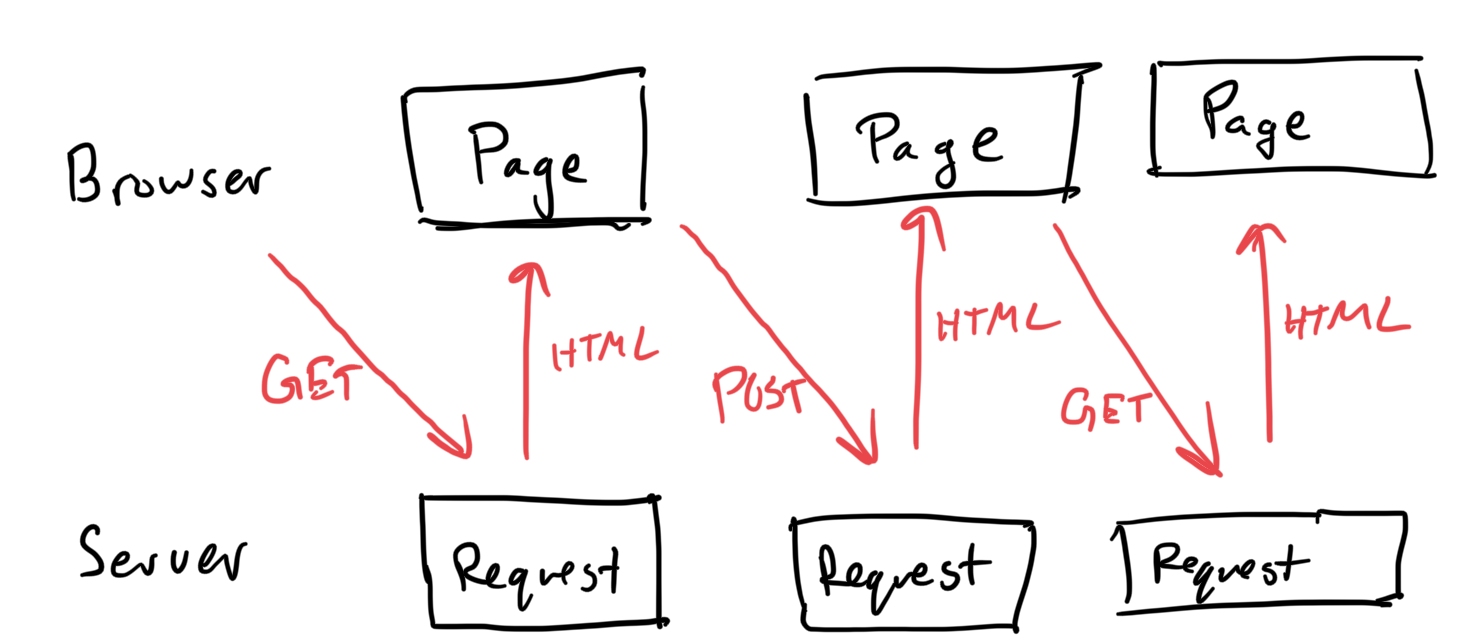
\includegraphics{im/forms-mpa.png}
\caption{The cycle of request and response for a multi-page application.}\label{fig:RequestResponse}
\end{figure}

Forms are a simple, minimal introduction to this cycle of request and
response and make a good introduction to how browser applications work.
They're also implemented in every browser and have been around for
decades. These days, many web applications use the form elements, but
replace synchronous \texttt{POST} requests with asynchronous ones driven by
Javascript,\footnote{In the early 2000s, the adoption of asynchronous
  HTTP requests sparked the wave of innovative new web applications
  called \href{https://en.wikipedia.org/wiki/Web_2.0}{Web~2.0}.} which
makes applications snappier by hiding the time to make the HTTP request.
In return for that snappiness, that JavaScript code must now handle
errors, validate inputs, and indicate loading time. In any case, both
synchronous and asynchronous uses of forms are based on the same
principles of client and server code.

\begin{bookblock}{further}
There are request types besides \texttt{GET} and \texttt{POST}, like
\href{https://developer.mozilla.org/en-US/docs/Web/HTTP/Methods/PUT}{\texttt{PUT}}
(create if non-existent) and
\href{https://developer.mozilla.org/en-US/docs/Web/HTTP/Methods/DELETE}{\texttt{DELETE}},
or the more obscure \texttt{CONNECT} and \texttt{TRACE}. In 2010 the
\href{https://developer.mozilla.org/en-US/docs/Web/HTTP/Methods/PATCH}{\texttt{PATCH}
method} was standardized in
\href{https://datatracker.ietf.org/doc/html/rfc5789}{RFC~5789}. New
methods were intended as a standard extension mechanism for HTTP, and
some protocols were built this way (like
\href{https://en.wikipedia.org/wiki/WebDAV}{WebDav}'s \texttt{PROPFIND}, \texttt{MOVE},
and \texttt{LOCK} methods), but this did not become an enduring way to extend the
web itself, and HTTP~2.0 and 3.0 did not add any new methods.
\end{bookblock}

\hypertarget{receiving-post-requests}{%
\section{Receiving \texttt{POST} Requests}\label{receiving-post-requests}}

To better understand the request/response cycle, let's write a simple
web server. It'll implement an online guest book,\footnote{They were
  very hip in the 1990s---comment threads from before there was anything
  to comment on.} kind of like an open, anonymous comment thread. Now,
this is a book on web \emph{browser} engineering, so I won't discuss web
server implementation that thoroughly. But I want you to see how the
server side of an application works.

A web server is a separate program from the web browser, so let's start
a new file. The server will need to:
\begin{itemize}
% \tightlist
\item
  open a socket and listen for connections;
\item
  parse HTTP requests it receives;
\item
  respond to those requests with an HTML web page.
\end{itemize}
Let's start by opening a socket. Like for the browser, we need to create
an internet streaming socket using TCP:
\begin{Shaded}
\begin{Highlighting}[]
\ImportTok{import}\NormalTok{ socket}
\NormalTok{s }\OperatorTok{=}\NormalTok{ socket.socket(}
\NormalTok{    family}\OperatorTok{=}\NormalTok{socket.AF\_INET,}
    \BuiltInTok{type}\OperatorTok{=}\NormalTok{socket.SOCK\_STREAM,}
\NormalTok{    proto}\OperatorTok{=}\NormalTok{socket.IPPROTO\_TCP)}
\NormalTok{s.setsockopt(socket.SOL\_SOCKET, socket.SO\_REUSEADDR, }\DecValTok{1}\NormalTok{)}
\end{Highlighting}
\end{Shaded}
The \texttt{setsockopt} call is optional. Normally, when a program has a
socket open and it crashes, your OS prevents that port from being
reused\footnote{When your process crashes, the computer on the end of
  the connection won't be informed immediately; if some other process
  opens the same port, it could receive data meant for the old, now-dead
  process.} for a short period. That's annoying when developing a
server; calling \texttt{setsockopt} with the \texttt{SO\_REUSEADDR}
option allows the OS to immediately reuse the port.

Now, with this socket, instead of calling \texttt{connect} (to connect
to some other server), we'll call \texttt{bind}, which waits for other
computers to connect:
\begin{Shaded}
\begin{Highlighting}[]
\NormalTok{s.bind((}\StringTok{\textquotesingle{}\textquotesingle{}}\NormalTok{, }\DecValTok{8000}\NormalTok{))}
\NormalTok{s.listen()}
\end{Highlighting}
\end{Shaded}
Let's look at the \texttt{bind} call first. Its first argument says who
should be allowed to make connections \emph{to} the server; the empty
string means that anyone can connect. The second argument is the port
others must use to talk to our server; I've chosen \texttt{8000}. I
can't use 80, because ports below 1024 require administrator privileges,
but you can pick something other than 8000 if, for whatever reason, port
8000 is taken on your machine.
Finally, after the \texttt{bind} call, the \texttt{listen} call tells
the OS that we're ready to accept connections.

To actually accept those connections, we enter a loop that runs once per
connection. At the top of the loop we call \texttt{s.accept} to wait for
a new connection:
\begin{Shaded}
\begin{Highlighting}[]
\ControlFlowTok{while} \VariableTok{True}\NormalTok{:}
\NormalTok{    conx, addr }\OperatorTok{=}\NormalTok{ s.accept()}
\NormalTok{    handle\_connection(conx)}
\end{Highlighting}
\end{Shaded}
That connection object is, confusingly, also a socket: it is the socket
corresponding to that one connection. We know what to do with those: we
read the contents and parse the HTTP message. But it's a little trickier
in the server than in the browser, because the server can't just read
from the socket until the connection closes---the browser is waiting for
the server and won't close the connection.
So, we've got to read from the socket line by line. First, we read the
request line:
\begin{Shaded}
\begin{Highlighting}[]
\KeywordTok{def}\NormalTok{ handle\_connection(conx):}
\NormalTok{    req }\OperatorTok{=}\NormalTok{ conx.makefile(}\StringTok{"b"}\NormalTok{)}
\NormalTok{    reqline }\OperatorTok{=}\NormalTok{ req.readline().decode(}\StringTok{\textquotesingle{}utf8\textquotesingle{}}\NormalTok{)}
\NormalTok{    method, url, version }\OperatorTok{=}\NormalTok{ reqline.split(}\StringTok{" "}\NormalTok{, }\DecValTok{2}\NormalTok{)}
    \ControlFlowTok{assert}\NormalTok{ method }\KeywordTok{in}\NormalTok{ [}\StringTok{"GET"}\NormalTok{, }\StringTok{"POST"}\NormalTok{]}
\end{Highlighting}
\end{Shaded}
Then we read the headers until we get to a blank line, accumulating the
headers in a dictionary:
\begin{Shaded}
\begin{Highlighting}[]
\KeywordTok{def}\NormalTok{ handle\_connection(conx):}
    \CommentTok{\# ...}
\NormalTok{    headers }\OperatorTok{=}\NormalTok{ \{\}}
    \ControlFlowTok{while} \VariableTok{True}\NormalTok{:}
\NormalTok{        line }\OperatorTok{=}\NormalTok{ req.readline().decode(}\StringTok{\textquotesingle{}utf8\textquotesingle{}}\NormalTok{)}
        \ControlFlowTok{if}\NormalTok{ line }\OperatorTok{==} \StringTok{\textquotesingle{}}\CharTok{\textbackslash{}r\textbackslash{}n}\StringTok{\textquotesingle{}}\NormalTok{: }\ControlFlowTok{break}
\NormalTok{        header, value }\OperatorTok{=}\NormalTok{ line.split(}\StringTok{":"}\NormalTok{, }\DecValTok{1}\NormalTok{)}
\NormalTok{        headers[header.casefold()] }\OperatorTok{=}\NormalTok{ value.strip()}
\end{Highlighting}
\end{Shaded}
Finally we read the body, but only when the \texttt{Content-Length}
header tells us how much of it to read (that's why that header is
mandatory on \texttt{POST} requests):
\begin{Shaded}
\begin{Highlighting}[]
\KeywordTok{def}\NormalTok{ handle\_connection(conx):}
    \CommentTok{\# ...}
    \ControlFlowTok{if} \StringTok{\textquotesingle{}content{-}length\textquotesingle{}} \KeywordTok{in}\NormalTok{ headers:}
\NormalTok{        length }\OperatorTok{=} \BuiltInTok{int}\NormalTok{(headers[}\StringTok{\textquotesingle{}content{-}length\textquotesingle{}}\NormalTok{])}
\NormalTok{        body }\OperatorTok{=}\NormalTok{ req.read(length).decode(}\StringTok{\textquotesingle{}utf8\textquotesingle{}}\NormalTok{)}
    \ControlFlowTok{else}\NormalTok{:}
\NormalTok{        body }\OperatorTok{=} \VariableTok{None}
\end{Highlighting}
\end{Shaded}

Now the server needs to generate a web page in response. We'll get to
that later; for now, just abstract that away behind a
\texttt{do\_request} call:
\begin{Shaded}
\begin{Highlighting}[]
\KeywordTok{def}\NormalTok{ handle\_connection(conx):}
    \CommentTok{\# ...}
\NormalTok{    status, body }\OperatorTok{=}\NormalTok{ do\_request(method, url, headers, body)}
\end{Highlighting}
\end{Shaded}
The server then sends this page back to the browser:
\begin{Shaded}
\begin{Highlighting}[]
\KeywordTok{def}\NormalTok{ handle\_connection(conx):}
    \CommentTok{\# ...}
\NormalTok{    response }\OperatorTok{=} \StringTok{"HTTP/1.0 }\SpecialCharTok{\{\}}\CharTok{\textbackslash{}r\textbackslash{}n}\StringTok{"}\NormalTok{.}\BuiltInTok{format}\NormalTok{(status)}
\NormalTok{    response }\OperatorTok{+=} \StringTok{"Content{-}Length: }\SpecialCharTok{\{\}}\CharTok{\textbackslash{}r\textbackslash{}n}\StringTok{"}\NormalTok{.}\BuiltInTok{format}\NormalTok{(}
        \BuiltInTok{len}\NormalTok{(body.encode(}\StringTok{"utf8"}\NormalTok{)))}
\NormalTok{    response }\OperatorTok{+=} \StringTok{"}\CharTok{\textbackslash{}r\textbackslash{}n}\StringTok{"} \OperatorTok{+}\NormalTok{ body}
\NormalTok{    conx.send(response.encode(}\StringTok{\textquotesingle{}utf8\textquotesingle{}}\NormalTok{))}
\NormalTok{    conx.close()}
\end{Highlighting}
\end{Shaded}

The architecture is summarized in Figure~\ref{fig:SimpleServer}. % This
Our implementation is all pretty bare-bones: our server doesn't check that the browser
is using HTTP~1.0 to talk to it, it doesn't send back any headers at all
except \texttt{Content-Length}, it doesn't support TLS, and so on.
Again: this is a web \emph{browser} book---it'll do.

\begin{figure}[tbp]
\centering
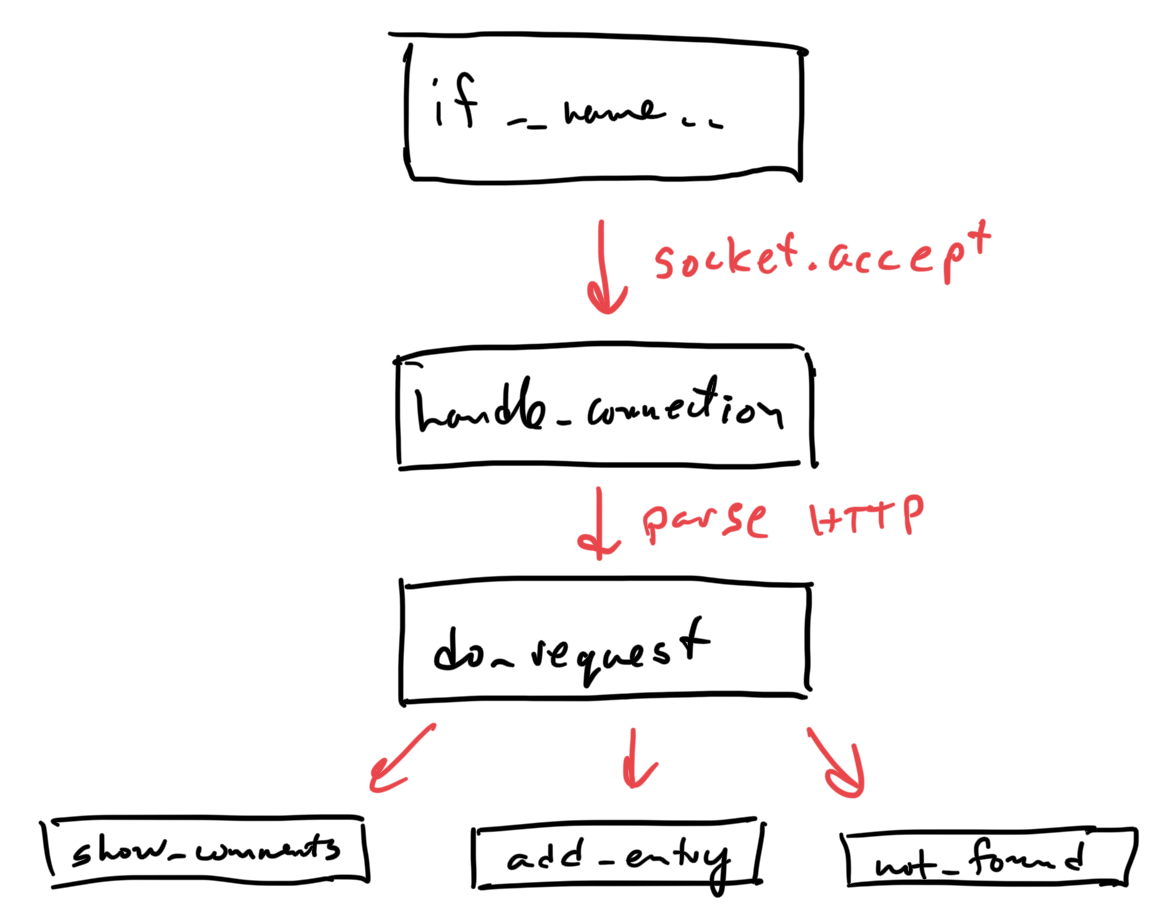
\includegraphics{im/forms-server.png}
\caption{The architecture of the simple web server in this chapter.}\label{fig:SimpleServer}
\end{figure}

\begin{bookblock}{further}
Ilya Grigorik's \href{https://hpbn.co}{\emph{High Performance Browser
Networking}} is an excellent deep dive into networking and how to
optimize for it in a web application. There are things the client can do
(make fewer requests, avoid polling, reuse connections) and things the
server can do (compression, protocol support, sharing domains).
\end{bookblock}

\hypertarget{generating-web-pages}{%
\section{Generating Web Pages}\label{generating-web-pages}}

So far, all of this server code is ``boilerplate''---any web application
will have similar code. What makes our server a guest book, on the other
hand, depends on what happens inside \texttt{do\_request}. It needs to
store the guest book state, generate HTML pages, and respond to
\texttt{POST} requests.

Let's store guest book entries in a Python list. Usually, web
applications use \emph{persistent} state, like a database, so that the
server can be restarted without losing state, but our guest book need
not be that resilient.
\begin{Shaded}
\begin{Highlighting}[]
\NormalTok{ENTRIES }\OperatorTok{=}\NormalTok{ [ }\StringTok{\textquotesingle{}Pavel was here\textquotesingle{}}\NormalTok{ ]}
\end{Highlighting}
\end{Shaded}
Next, \texttt{do\_request} has to output HTML that shows those entries:
\begin{Shaded}
\begin{Highlighting}[]
\KeywordTok{def}\NormalTok{ do\_request(method, url, headers, body):}
\NormalTok{    out }\OperatorTok{=} \StringTok{"\textless{}!doctype html\textgreater{}"}
    \ControlFlowTok{for}\NormalTok{ entry }\KeywordTok{in}\NormalTok{ ENTRIES:}
\NormalTok{        out }\OperatorTok{+=} \StringTok{"\textless{}p\textgreater{}"} \OperatorTok{+}\NormalTok{ entry }\OperatorTok{+} \StringTok{"\textless{}/p\textgreater{}"}
    \ControlFlowTok{return} \StringTok{"200 OK"}\NormalTok{, out}
\end{Highlighting}
\end{Shaded}
This is definitely ``minimal'' HTML, so it's a good thing our browser
will insert implicit tags and has some default styles! You can test it
out by running this minimal web server and, while it's running, direct
your browser to \texttt{http://localhost:8000/}, where
\texttt{localhost} is what your computer calls itself and \texttt{8000}
is the port we chose earlier. You should see one guest book entry.

By the way, while you're debugging this web server, it's probably better
to use a real web browser, instead of this book's browser, to interact
with it. That way you don't have to worry about browser bugs while you
work on server bugs. But this server does support both real and toy
browsers.

We'll use forms to let visitors write in the guest book:
\begin{Shaded}
\begin{Highlighting}[]
\KeywordTok{def}\NormalTok{ do\_request(method, url, headers, body):}
    \CommentTok{\# ...}
\NormalTok{    out }\OperatorTok{+=} \StringTok{"\textless{}form action=add method=post\textgreater{}"}
\NormalTok{    out }\OperatorTok{+=}   \StringTok{"\textless{}p\textgreater{}\textless{}input name=guest\textgreater{}\textless{}/p\textgreater{}"}
\NormalTok{    out }\OperatorTok{+=}   \StringTok{"\textless{}p\textgreater{}\textless{}button\textgreater{}Sign the book!\textless{}/button\textgreater{}\textless{}/p\textgreater{}"}
\NormalTok{    out }\OperatorTok{+=} \StringTok{"\textless{}/form\textgreater{}"}
    \CommentTok{\# ...}
\end{Highlighting}
\end{Shaded}
When this form is submitted, the browser will send a \texttt{POST}
request to \texttt{http://localhost:8000/add}. So the server needs to
react to these submissions. That means \texttt{do\_request} will field
two kinds of requests: regular browsing and form submissions. Let's
separate the two kinds of requests into different functions.

First, rename the current \texttt{do\_request} to
\texttt{show\_comments}:
\begin{Shaded}
\begin{Highlighting}[]
\KeywordTok{def}\NormalTok{ show\_comments():}
    \CommentTok{\# ...}
    \ControlFlowTok{return}\NormalTok{ out}
\end{Highlighting}
\end{Shaded}
This then frees up the \texttt{do\_request} function to figure out which
function to call for which request:
\begin{Shaded}
\begin{Highlighting}[]
\KeywordTok{def}\NormalTok{ do\_request(method, url, headers, body):}
    \ControlFlowTok{if}\NormalTok{ method }\OperatorTok{==} \StringTok{"GET"} \KeywordTok{and}\NormalTok{ url }\OperatorTok{==} \StringTok{"/"}\NormalTok{:}
        \ControlFlowTok{return} \StringTok{"200 OK"}\NormalTok{, show\_comments()}
    \ControlFlowTok{elif}\NormalTok{ method }\OperatorTok{==} \StringTok{"POST"} \KeywordTok{and}\NormalTok{ url }\OperatorTok{==} \StringTok{"/add"}\NormalTok{:}
\NormalTok{        params }\OperatorTok{=}\NormalTok{ form\_decode(body)}
        \ControlFlowTok{return} \StringTok{"200 OK"}\NormalTok{, add\_entry(params)}
    \ControlFlowTok{else}\NormalTok{:}
        \ControlFlowTok{return} \StringTok{"404 Not Found"}\NormalTok{, not\_found(url, method)}
\end{Highlighting}
\end{Shaded}

When a \texttt{POST} request to \texttt{/add} comes in, the first step
is to decode the request body:
\begin{Shaded}
\begin{Highlighting}[]
\KeywordTok{def}\NormalTok{ form\_decode(body):}
\NormalTok{    params }\OperatorTok{=}\NormalTok{ \{\}}
    \ControlFlowTok{for}\NormalTok{ field }\KeywordTok{in}\NormalTok{ body.split(}\StringTok{"\&"}\NormalTok{):}
\NormalTok{        name, value }\OperatorTok{=}\NormalTok{ field.split(}\StringTok{"="}\NormalTok{, }\DecValTok{1}\NormalTok{)}
\NormalTok{        name }\OperatorTok{=}\NormalTok{ urllib.parse.unquote\_plus(name)}
\NormalTok{        value }\OperatorTok{=}\NormalTok{ urllib.parse.unquote\_plus(value)}
\NormalTok{        params[name] }\OperatorTok{=}\NormalTok{ value}
    \ControlFlowTok{return}\NormalTok{ params}
\end{Highlighting}
\end{Shaded}
Note that I use \texttt{unquote\_plus} instead of \texttt{unquote},
because browsers may also use a plus sign to encode a space. The
\texttt{add\_entry} function then looks up the \texttt{guest} parameter
and adds its content as a new guest book entry:
\begin{Shaded}
\begin{Highlighting}[]
\KeywordTok{def}\NormalTok{ add\_entry(params):}
    \ControlFlowTok{if} \StringTok{\textquotesingle{}guest\textquotesingle{}} \KeywordTok{in}\NormalTok{ params:}
\NormalTok{        ENTRIES.append(params[}\StringTok{\textquotesingle{}guest\textquotesingle{}}\NormalTok{])}
    \ControlFlowTok{return}\NormalTok{ show\_comments()}
\end{Highlighting}
\end{Shaded}

I've also added a ``404'' response. Fitting the austere stylings of our
guest book, here's the 404 page:
\begin{Shaded}
\begin{Highlighting}[]
\KeywordTok{def}\NormalTok{ not\_found(url, method):}
\NormalTok{    out }\OperatorTok{=} \StringTok{"\textless{}!doctype html\textgreater{}"}
\NormalTok{    out }\OperatorTok{+=} \StringTok{"\textless{}h1\textgreater{}}\SpecialCharTok{\{\}}\StringTok{ }\SpecialCharTok{\{\}}\StringTok{ not found!\textless{}/h1\textgreater{}"}\NormalTok{.}\BuiltInTok{format}\NormalTok{(method, url)}
    \ControlFlowTok{return}\NormalTok{ out}
\end{Highlighting}
\end{Shaded}

Try it! You should be able to restart the server, open it in your
browser, and update the guest book a few times. You should also be able
to use the guest book from a real web browser.

\begin{bookblock}{further}
Typically, connection handling and request routing is handled by a web
framework; this book, for example, uses
\href{https://bottlepy.org/docs/dev/}{bottle.py}. Frameworks parse
requests into convenient data structures, route requests to the right
handler, and can also provide tools like HTML templates, session
handling, database access, input validation, and API generation.
\end{bookblock}

\hypertarget{summary}{%
\section{Summary}\label{SendingInformation-summary}}

With this chapter we're starting to transform our browser into an
application platform. We've added:
\begin{itemize}
%\tightlist
\item
  layout objects for input areas and buttons;
\item
  clicking on buttons and typing into input areas;
\item
  hierarchical focus handling;
\item
  form submission with HTTP \texttt{POST}.
\end{itemize}
Plus, our browser now has a little web server friend. That's going to be
handy as we add more interactive features to the browser.

\hypertarget{outline}{%
\section{Outline}\label{SendingInformation-outline}}

The complete set of functions, classes, and methods in our browser
should now look something like this:
\begin{Shaded}
\begin{Highlighting}[]
\NormalTok{WIDTH}
\NormalTok{HEIGHT}
\NormalTok{HSTEP}
\NormalTok{VSTEP}
\NormalTok{SCROLL\_STEP}
\NormalTok{FONTS}
\KeywordTok{def}\NormalTok{ get\_font(size, weight, slant)}
\KeywordTok{class}\NormalTok{ Text:}
    \KeywordTok{def} \FunctionTok{\_\_init\_\_}\NormalTok{(text, parent)}
    \KeywordTok{def} \FunctionTok{\_\_repr\_\_}\NormalTok{()}
\KeywordTok{class}\NormalTok{ Element:}
    \KeywordTok{def} \FunctionTok{\_\_init\_\_}\NormalTok{(tag, attributes, parent)}
    \KeywordTok{def} \FunctionTok{\_\_repr\_\_}\NormalTok{()}
\KeywordTok{def}\NormalTok{ print\_tree(node, indent)}
\KeywordTok{class}\NormalTok{ HTMLParser:}
    \KeywordTok{def} \FunctionTok{\_\_init\_\_}\NormalTok{(body)}
    \KeywordTok{def}\NormalTok{ parse()}
    \KeywordTok{def}\NormalTok{ get\_attributes(text)}
    \KeywordTok{def}\NormalTok{ add\_text(text)}
\NormalTok{    SELF\_CLOSING\_TAGS}
    \KeywordTok{def}\NormalTok{ add\_tag(tag)}
\NormalTok{    HEAD\_TAGS}
    \KeywordTok{def}\NormalTok{ implicit\_tags(tag)}
    \KeywordTok{def}\NormalTok{ finish()}
\NormalTok{BLOCK\_ELEMENTS}
\KeywordTok{class}\NormalTok{ DocumentLayout:}
    \KeywordTok{def} \FunctionTok{\_\_init\_\_}\NormalTok{(node)}
    \KeywordTok{def}\NormalTok{ layout()}
    \KeywordTok{def}\NormalTok{ paint()}
    \KeywordTok{def}\NormalTok{ should\_paint()}
\KeywordTok{class}\NormalTok{ CSSParser:}
    \KeywordTok{def} \FunctionTok{\_\_init\_\_}\NormalTok{(s)}
    \KeywordTok{def}\NormalTok{ whitespace()}
    \KeywordTok{def}\NormalTok{ literal(literal)}
    \KeywordTok{def}\NormalTok{ word()}
    \KeywordTok{def}\NormalTok{ pair()}
    \KeywordTok{def}\NormalTok{ ignore\_until(chars)}
    \KeywordTok{def}\NormalTok{ body()}
    \KeywordTok{def}\NormalTok{ selector()}
    \KeywordTok{def}\NormalTok{ parse()}
\KeywordTok{class}\NormalTok{ TagSelector:}
    \KeywordTok{def} \FunctionTok{\_\_init\_\_}\NormalTok{(tag)}
    \KeywordTok{def}\NormalTok{ matches(node)}
\KeywordTok{class}\NormalTok{ DescendantSelector:}
    \KeywordTok{def} \FunctionTok{\_\_init\_\_}\NormalTok{(ancestor, descendant)}
    \KeywordTok{def}\NormalTok{ matches(node)}
\NormalTok{INHERITED\_PROPERTIES}
\KeywordTok{def}\NormalTok{ style(node, rules)}
\KeywordTok{def}\NormalTok{ cascade\_priority(rule)}
\KeywordTok{class}\NormalTok{ DrawText:}
    \KeywordTok{def} \FunctionTok{\_\_init\_\_}\NormalTok{(x1, y1, text, font, color)}
    \KeywordTok{def}\NormalTok{ execute(scroll, canvas)}
\KeywordTok{class}\NormalTok{ URL:}
    \KeywordTok{def} \FunctionTok{\_\_init\_\_}\NormalTok{(url)}
    \KeywordTok{def}\NormalTok{ request(payload)}
    \KeywordTok{def}\NormalTok{ resolve(url)}
\KeywordTok{def}\NormalTok{ tree\_to\_list(tree, }\NormalTok{list}\NormalTok{)}
\KeywordTok{class}\NormalTok{ DrawLine:}
    \KeywordTok{def} \FunctionTok{\_\_init\_\_}\NormalTok{(x1, y1, x2, y2, color, thickness)}
    \KeywordTok{def}\NormalTok{ execute(scroll, canvas)}
\KeywordTok{class}\NormalTok{ DrawOutline:}
    \KeywordTok{def} \FunctionTok{\_\_init\_\_}\NormalTok{(rect, color, thickness)}
    \KeywordTok{def}\NormalTok{ execute(scroll, canvas)}
\KeywordTok{class}\NormalTok{ BlockLayout:}
    \KeywordTok{def} \FunctionTok{\_\_init\_\_}\NormalTok{(node, parent, previous)}
    \KeywordTok{def}\NormalTok{ token(tok)}
    \KeywordTok{def}\NormalTok{ word(node, word)}
    \KeywordTok{def}\NormalTok{ flush()}
    \KeywordTok{def}\NormalTok{ recurse(node)}
    \KeywordTok{def}\NormalTok{ layout()}
    \KeywordTok{def}\NormalTok{ layout\_mode()}
    \KeywordTok{def}\NormalTok{ paint()}
    \KeywordTok{def}\NormalTok{ new\_line()}
    \KeywordTok{def}\NormalTok{ self\_rect()}
    \KeywordTok{def} \NormalTok{input}\NormalTok{(node)}
    \KeywordTok{def}\NormalTok{ should\_paint()}
\KeywordTok{class}\NormalTok{ LineLayout:}
    \KeywordTok{def} \FunctionTok{\_\_init\_\_}\NormalTok{(node, parent, previous)}
    \KeywordTok{def}\NormalTok{ layout()}
    \KeywordTok{def}\NormalTok{ paint()}
    \KeywordTok{def}\NormalTok{ should\_paint()}
\KeywordTok{class}\NormalTok{ TextLayout:}
    \KeywordTok{def} \FunctionTok{\_\_init\_\_}\NormalTok{(node, word, parent, previous)}
    \KeywordTok{def}\NormalTok{ layout()}
    \KeywordTok{def}\NormalTok{ paint()}
    \KeywordTok{def}\NormalTok{ should\_paint()}
\KeywordTok{class}\NormalTok{ Tab:}
    \KeywordTok{def} \FunctionTok{\_\_init\_\_}\NormalTok{(tab\_height)}
    \KeywordTok{def}\NormalTok{ load(url, payload)}
    \KeywordTok{def}\NormalTok{ draw(canvas, offset)}
    \KeywordTok{def}\NormalTok{ scrolldown()}
    \KeywordTok{def}\NormalTok{ click(x, y)}
    \KeywordTok{def}\NormalTok{ go\_back()}
    \KeywordTok{def}\NormalTok{ render()}
    \KeywordTok{def}\NormalTok{ submit\_form(elt)}
    \KeywordTok{def}\NormalTok{ keypress(char)}
\KeywordTok{class}\NormalTok{ Browser:}
    \KeywordTok{def} \FunctionTok{\_\_init\_\_}\NormalTok{()}
    \KeywordTok{def}\NormalTok{ handle\_down(e)}
    \KeywordTok{def}\NormalTok{ handle\_click(e)}
    \KeywordTok{def}\NormalTok{ handle\_key(e)}
    \KeywordTok{def}\NormalTok{ handle\_enter(e)}
    \KeywordTok{def}\NormalTok{ new\_tab(url)}
    \KeywordTok{def}\NormalTok{ draw()}
\KeywordTok{class}\NormalTok{ Chrome:}
    \KeywordTok{def} \FunctionTok{\_\_init\_\_}\NormalTok{(browser)}
    \KeywordTok{def}\NormalTok{ tab\_rect(i)}
    \KeywordTok{def}\NormalTok{ paint()}
    \KeywordTok{def}\NormalTok{ click(x, y)}
    \KeywordTok{def}\NormalTok{ keypress(char)}
    \KeywordTok{def}\NormalTok{ enter()}
    \KeywordTok{def}\NormalTok{ blur()}
\KeywordTok{class}\NormalTok{ DrawRect:}
    \KeywordTok{def} \FunctionTok{\_\_init\_\_}\NormalTok{(rect, color)}
    \KeywordTok{def}\NormalTok{ execute(scroll, canvas)}
\KeywordTok{class}\NormalTok{ Rect:}
    \KeywordTok{def} \FunctionTok{\_\_init\_\_}\NormalTok{(left, top, right, bottom)}
    \KeywordTok{def}\NormalTok{ containsPoint(x, y)}
\NormalTok{DEFAULT\_STYLE\_SHEET}
\NormalTok{INPUT\_WIDTH\_PX}
\KeywordTok{class}\NormalTok{ InputLayout:}
    \KeywordTok{def} \FunctionTok{\_\_init\_\_}\NormalTok{(node, parent, previous)}
    \KeywordTok{def}\NormalTok{ layout()}
    \KeywordTok{def}\NormalTok{ should\_paint()}
    \KeywordTok{def}\NormalTok{ self\_rect()}
    \KeywordTok{def}\NormalTok{ paint()}
    \KeywordTok{def} \FunctionTok{\_\_repr\_\_}\NormalTok{()}
\KeywordTok{def}\NormalTok{ paint\_tree(layout\_object, display\_list)}
\end{Highlighting}
\end{Shaded}

There's also a server now, but it's much simpler:
\begin{Shaded}
\begin{Highlighting}[]
\KeywordTok{def}\NormalTok{ handle\_connection(conx)}
\KeywordTok{def}\NormalTok{ do\_request(method, url, headers, body)}
\KeywordTok{def}\NormalTok{ form\_decode(body)}
\NormalTok{ENTRIES}
\KeywordTok{def}\NormalTok{ show\_comments()}
\KeywordTok{def}\NormalTok{ not\_found(url, method)}
\KeywordTok{def}\NormalTok{ add\_entry(params)}
\end{Highlighting}
\end{Shaded}

\hypertarget{exercises}{%
\section{Exercises}\label{SendingInformation-exercises}}
\begin{enumerate}[label=\thechapter-\arabic*]
\item \emph{Enter key.} In most browsers, if you hit the ``Enter'' or
``Return'' key while inside a text entry, that submits the form that the
text entry was in. Add this feature to your browser.

\item \emph{\texttt{GET} forms.} Forms can be submitted via \texttt{GET} requests as well as
\texttt{POST} requests. In \texttt{GET} requests, the form-encoded data is pasted onto the
end of the URL, separated from the path by a question mark, like
\texttt{/search?q=hi}; \texttt{GET} form submissions have no body. Implement \texttt{GET}
form submissions.

\item \emph{Blurring.} Right now, if you click inside a text entry, and then
inside the address bar, two cursors will appear on the screen. To fix
this, add a \texttt{blur} method to each \texttt{Tab} which unfocuses
anything that is focused, and call it before changing focus.

\item \emph{Check boxes.} In HTML, \texttt{input} elements have a
\texttt{type} attribute. When set to \texttt{checkbox}, the
\texttt{input} element looks like a checkbox; it's checked if the
\texttt{checked} attribute is set, and unchecked otherwise.\footnote{Technically,
  the \texttt{checked} attribute
  \href{https://developer.mozilla.org/en-US/docs/Web/HTML/Element/input/checkbox\#attr-checked}{only
  affects the state of the checkbox when the page loads}; checking and
  unchecking a checkbox does not affect this attribute but instead
  manipulates internal state.} When the form is submitted, a checkbox's
\texttt{name=value} pair is included only if the checkbox is checked.
(If the checkbox has no \texttt{value} attribute, the default is the
string \texttt{on}.)

\item\label{ex:Resubmit} \emph{Resubmit requests.} One reason to
  separate \texttt{GET} and \texttt{POST} requests
is that \texttt{GET} requests are supposed to be \emph{idempotent} (read-only,
basically) while \texttt{POST} requests are assumed to change the web server
state. That means that going ``back'' to a \texttt{GET} request (making the
request again) is safe, while going ``back'' to a \texttt{POST} request is a bad
idea. Change the browser history to record what method was used to
access each URL, and the \texttt{POST} body if one was used. When you go back to
a \texttt{POST}-ed URL, ask the user if they want to resubmit the form. Don't go
back if they say no; if they say yes, submit a \texttt{POST} request with the
same body as before.

\item \emph{Message board.} Right now our web server is a simple guest book.
Extend it into a simple message board by adding support for topics. Each
topic should have its own URL and its own list of messages. So, for
example, \texttt{/cooking} should be a page of posts (about cooking) and
comments submitted through the form on that page should only show up
when you go to \texttt{/cooking}, not when you go to \texttt{/cars}.
Make the home page, from \texttt{/}, list the available topics with a
link to each topic's page. Make it possible for users to add new topics.

\item \emph{Persistence.} Back the server's list of guest book entries with a
file, so that when the server is restarted it doesn't lose data.

\item\label{ex:RichButtons} \emph{Rich buttons.} Make it possible for a button to contain arbitrary
elements as children, and render them correctly. The children should be
contained inside the button instead of spilling out---this can make a button
really tall. Think about edge cases, like a button that contains another
button, an input area, or a link, and test real browsers to see what
they do.

\item \emph{HTML chrome.} Browser chrome is quite complicated in real
browsers, with tricky details such as font sizes, padding, outlines,
shadows, icons, and so on. This makes it tempting to try to reuse our
layout engine for it. Implement this, using
\texttt{\textless{}button\textgreater{}} elements for the new tab and
back buttons, an \texttt{\textless{}input\textgreater{}} element for the
address bar, and \texttt{\textless{}a\textgreater{}} elements for the
tab names. It won't look exactly the same as the current
chrome---outline will have to wait for % \href{accessibility.md}{Chapter 14}
Chapter~\ref{ch:Accessible}, for example---but if you adjust the default CSS you should be able
to make it look passable.\footnote{Real browsers have in fact gone down
  this implementation path multiple times, building layout engines for
  the browser chrome that are heavily inspired by or reuse pieces of the
  main web layout engine.
  \href{https://en.wikipedia.org/wiki/XUL}{Firefox had one}, and
  \href{https://www.chromium.org/developers/webui/}{Chrome has one}.
  However, because it's so important for the browser chrome to be very
  fast and responsive to draw, such approaches have had mixed success.}
\end{enumerate}

\ifprintedoutput
\theendnotes
\setcounter{endnote}{0}
\fi

\chapter{Running Interactive Scripts}\label{ch:InteractiveScripts}
The first web applications were like % \href{forms.md}{last
the previous chapter's
guest book, with the server generating new web pages for every user
action. But in the early 2000s, JavaScript-enhanced web applications,
which can update pages dynamically and respond immediately to user
actions, took their place. Let's add support for this key web technology
to our browser.

\hypertarget{installing-dukpy}{%
\section{Installing DukPy}\label{installing-dukpy}}

Actually writing a JavaScript\index{JavaScript} interpreter is beyond
the scope of this book,\footnote{But check out a book on programming
  language implementation if it sounds interesting!} so this chapter
uses the \texttt{dukpy} library for executing JavaScript.

\href{https://github.com/amol-/dukpy}{DukPy}\index{DukPy} wraps a
JavaScript interpreter called \href{https://duktape.org}{Duktape}. The
most famous JavaScript interpreters are those used in browsers:
TraceMonkey (Firefox), JavaScriptCore (Safari), and V8 (Chrome). Unlike
those implementations, which are extremely fast but also extremely
complex, Duktape aims to be simple and extensible, and is usually
embedded inside a larger C or C++ project.\footnote{For example, in a
  video game the high-speed graphics code is usually written in C or C++,
  but the actual plot of the game is usually written in a higher-level
  language like JavaScript.}

Like other JavaScript engines, DukPy not only executes JavaScript code,
but also allows it to call \emph{exported} Python functions. We'll be
using this feature to allow JavaScript code to modify the web page it's
running on.

The first step to using DukPy is installing it. On most machines,
including on Windows, macOS, and Linux systems, you should be able to do
this with:
\begin{bookblock*}{notcode}
\begin{Shaded}
\begin{Highlighting}[]
\NormalTok{python3 {-}m pip install dukpy}
\end{Highlighting}
\end{Shaded}
\end{bookblock*}

\begin{bookblock}{installation}
If you have a really old version of Python, you might need to install
the \texttt{pip} package first, possibly using a command line
\texttt{easy\_install}. If you do your Python programming through an
integrated development environment (IDE), you may need to use your IDE's package installer. If nothing else
works, you can build \href{https://github.com/amol-/dukpy}{from source}.

If you're following along in something other than Python, you might need
to skip this chapter, though you could try binding directly to the
\texttt{duktape} library that \texttt{dukpy} uses.
\end{bookblock}

To test whether you installed DukPy correctly, execute this:
\begin{bookblock*}{notcode}
\begin{Shaded}
\begin{Highlighting}[]
\ImportTok{import}\NormalTok{ dukpy}
\NormalTok{dukpy.evaljs(}\StringTok{"2 + 2"}\NormalTok{)}
\end{Highlighting}
\end{Shaded}
\end{bookblock*}
\noindent If you get an error on the first line, you probably failed to install
DukPy.\footnote{Or, on my Linux machine, I sometimes get errors due to
  file ownership. You may have to do some sleuthing.} If you get an
error, or a segfault, on the second line, there's a chance that Duktape
failed to compile, or maybe doesn't support your system, and you might
need to debug further.

\begin{bookblock}{quirk}
Note to JavaScript experts: Dukpy does not implement newer syntax like
\texttt{let} and \texttt{const} or arrow functions. In keeping with this
book's aesthetics, you'll need to use old-school JavaScript from the
turn of the century.
\end{bookblock}

\hypertarget{running-javascript-code}{%
\section{Running JavaScript Code}\label{running-javascript-code}}

The test above shows how you run JavaScript code in DukPy: you just call
\texttt{evaljs}! Let's put this newfound knowledge to work in our
browser.

On the web, JavaScript is found in
\texttt{\textless{}script\textgreater{}} tags. Normally, a
\texttt{\textless{}script\textgreater{}} tag has a \texttt{src}
attribute with a relative URL that points to a JavaScript file, much
like with CSS files. A \texttt{\textless{}script\textgreater{}} tag
could also contain JavaScript source code between the start and end tag,
but we won't implement that.\footnote{It's a challenge for parsing,
  since it's hard to avoid less-than and greater-than signs in
  JavaScript code.}

Finding and downloading those scripts is similar to what we did for CSS.
First, we need to find all of the scripts:
\begin{Shaded}
\begin{Highlighting}[]
\KeywordTok{class}\NormalTok{ Tab:}
    \KeywordTok{def}\NormalTok{ load(}\VariableTok{self}\NormalTok{, url, payload}\OperatorTok{=}\VariableTok{None}\NormalTok{):}
        \CommentTok{\# ...}
\NormalTok{        scripts }\OperatorTok{=}\NormalTok{ [node.attributes[}\StringTok{"src"}\NormalTok{] }\ControlFlowTok{for}\NormalTok{ node}
                   \KeywordTok{in}\NormalTok{ tree\_to\_list(}\VariableTok{self}\NormalTok{.nodes, [])}
                   \ControlFlowTok{if} \BuiltInTok{isinstance}\NormalTok{(node, Element)}
                   \KeywordTok{and}\NormalTok{ node.tag }\OperatorTok{==} \StringTok{"script"}
                   \KeywordTok{and} \StringTok{"src"} \KeywordTok{in}\NormalTok{ node.attributes]}
        \CommentTok{\# ...}
\end{Highlighting}
\end{Shaded}
Next, we run all of the scripts:
\begin{Shaded}
\begin{Highlighting}[]
\KeywordTok{def}\NormalTok{ load(}\VariableTok{self}\NormalTok{, url, payload}\OperatorTok{=}\VariableTok{None}\NormalTok{):}
    \CommentTok{\# ...}
    \ControlFlowTok{for}\NormalTok{ script }\KeywordTok{in}\NormalTok{ scripts:}
\NormalTok{        script\_url }\OperatorTok{=}\NormalTok{ url.resolve(script)}
        \ControlFlowTok{try}\NormalTok{:}
\NormalTok{            body }\OperatorTok{=}\NormalTok{ script\_url.request()}
        \ControlFlowTok{except}\NormalTok{:}
            \ControlFlowTok{continue}
        \BuiltInTok{print}\NormalTok{(}\StringTok{"Script returned: "}\NormalTok{, dukpy.evaljs(body))}
    \CommentTok{\# ...}
\end{Highlighting}
\end{Shaded}
This should run before styling and layout. To try it out, create a
simple web page with a \texttt{script} tag:
\begin{bookblock*}{notcode}
\begin{Shaded}
\begin{Highlighting}[]
\KeywordTok{\textless{}script} \ErrorTok{src}\OtherTok{=}\StringTok{test.js}\KeywordTok{\textgreater{}\textless{}/script\textgreater{}}
\end{Highlighting}
\end{Shaded}
\end{bookblock*}
\noindent Then write a super simple script to \texttt{test.js}, maybe this:
\begin{bookblock*}{notcode}
\begin{Shaded}
\begin{Highlighting}[]
\KeywordTok{var}\NormalTok{ x }\OperatorTok{=} \DecValTok{2}
\NormalTok{x }\OperatorTok{+}\NormalTok{ x}
\end{Highlighting}
\end{Shaded}
\end{bookblock*}
\noindent Point your browser at that page, and you should see:
\begin{bookblock*}{notcode}
\begin{verbatim}
Script returned: 4
\end{verbatim}
\end{bookblock*}
\noindent That's your browser running its first bit of JavaScript!

\begin{bookblock}{further}
Actually, real browsers run JavaScript code as soon as the browser
\emph{parses} the \texttt{\textless{}script\textgreater{}} tag, not
after the whole page is parsed. Or, at least, that is the default; there
are
\href{https://html.spec.whatwg.org/multipage/scripting.html\#the-script-element}{many
options}. What our browser does is what a real browser does when the
\href{https://developer.mozilla.org/en-US/docs/Web/HTML/Element/script\#attr-defer}{\texttt{defer}}
attribute is set. The default behavior is
\href{https://developer.mozilla.org/en-US/docs/Glossary/speculative_parsing}{much
trickier} to implement efficiently.
\end{bookblock}

\hypertarget{exporting-functions}{%
\section{Exporting Functions}\label{exporting-functions}}

Right now, our browser just prints the last expression in a script; but
in a real browser scripts must call the \texttt{console.log} function to
print. To support that, we will need to \emph{export a function} from
Python into JavaScript. We'll be exporting a lot of functions, so to
avoid polluting the \texttt{Tab} object with many new methods, let's put
this code in a new \texttt{JSContext} class:
\begin{Shaded}
\begin{Highlighting}[]
\KeywordTok{class}\NormalTok{ JSContext:}
    \KeywordTok{def} \FunctionTok{\_\_init\_\_}\NormalTok{(}\VariableTok{self}\NormalTok{):}
        \VariableTok{self}\NormalTok{.interp }\OperatorTok{=}\NormalTok{ dukpy.JSInterpreter()}

    \KeywordTok{def}\NormalTok{ run(}\VariableTok{self}\NormalTok{, code):}
        \ControlFlowTok{return} \VariableTok{self}\NormalTok{.interp.evaljs(code)}
\end{Highlighting}
\end{Shaded}
DukPy's \texttt{JSInterpreter} object stores the values of all the
JavaScript variables, and lets us run multiple JavaScript snippets and
share variable values and other state between them.

We create this new \texttt{JSContext} object while loading the page:
\begin{Shaded}
\begin{Highlighting}[]
\KeywordTok{class}\NormalTok{ Tab:}
    \KeywordTok{def}\NormalTok{ load(}\VariableTok{self}\NormalTok{, url, payload}\OperatorTok{=}\VariableTok{None}\NormalTok{):}
        \CommentTok{\# ...}
        \VariableTok{self}\NormalTok{.js }\OperatorTok{=}\NormalTok{ JSContext()}
        \ControlFlowTok{for}\NormalTok{ script }\KeywordTok{in}\NormalTok{ scripts:}
            \CommentTok{\# ...}
            \VariableTok{self}\NormalTok{.js.run(body)}
\end{Highlighting}
\end{Shaded}

As a side benefit of using one \texttt{JSContext} for all scripts, it is
now possible to run two scripts and have one of them define a variable
that the other uses, say on a page like this:
\begin{bookblock*}{notcode}
\begin{Shaded}
\begin{Highlighting}[]
\DataTypeTok{\textless{}}\KeywordTok{script}\OtherTok{ src}\OperatorTok{=}\StringTok{a.js}\DataTypeTok{\textgreater{}\textless{}/}\KeywordTok{script}\DataTypeTok{\textgreater{}}
\DataTypeTok{\textless{}}\KeywordTok{script}\OtherTok{ src}\OperatorTok{=}\StringTok{b.js}\DataTypeTok{\textgreater{}\textless{}/}\KeywordTok{script}\DataTypeTok{\textgreater{}}
\end{Highlighting}
\end{Shaded}
\end{bookblock*}
\noindent Suppose \texttt{a.js} is ``\texttt{var\ x\ =\ 2;}'' and \texttt{b.js} is
``\texttt{console.log(x\ +\ x)}''; the variable \texttt{x} is set in
\texttt{a.js} but used in \texttt{b.js}. In real web browsers, that's
important, since one script might define library functions that another
script wants to call.

Now, to allow JavaScript to interact with the outside world, DukPy
allows us to ``export'' functions to it. For example, we can export
Python's \texttt{print} function like so:
\begin{Shaded}
\begin{Highlighting}[]
\KeywordTok{class}\NormalTok{ JSContext:}
    \KeywordTok{def} \FunctionTok{\_\_init\_\_}\NormalTok{(}\VariableTok{self}\NormalTok{):}
        \CommentTok{\# ...}
        \VariableTok{self}\NormalTok{.interp.export\_function(}\StringTok{"log"}\NormalTok{, }\BuiltInTok{print}\NormalTok{)}
\end{Highlighting}
\end{Shaded}
We can call an exported function from JavaScript using Dukpy's
\texttt{call\_python} function. For example:
\begin{bookblock*}{notcode}
\begin{Shaded}
\begin{Highlighting}[]
\FunctionTok{call\_python}\NormalTok{(}\StringTok{"log"}\OperatorTok{,} \StringTok{"Hi from JS"}\NormalTok{)}
\end{Highlighting}
\end{Shaded}
\end{bookblock*}
\noindent When this JavaScript code runs, Dukpy converts the JavaScript string
\texttt{"Hi\ from\ JS"} into a Python string,\footnote{This conversion
  works for numbers, strings, and booleans, plus arrays and dictionaries
  thereof, but not with fancy objects.} and then passes that Python
string to the \texttt{print} function we exported. Then \texttt{print}
prints that string.

Since we ultimately want a
\href{https://developer.mozilla.org/en-US/docs/Web/API/console/log}{\texttt{console.log}}
function, not a \texttt{call\_python} function, we need to define a
\texttt{console} object and then give it a \texttt{log} property. We can
do that \emph{in JavaScript}:
\begin{bookblock*}{notcode}
\begin{Shaded}
\begin{Highlighting}[]
\BuiltInTok{console} \OperatorTok{=}\NormalTok{ \{ }\DataTypeTok{log}\OperatorTok{:} \KeywordTok{function}\NormalTok{(x) \{ }\FunctionTok{call\_python}\NormalTok{(}\StringTok{"log"}\OperatorTok{,}\NormalTok{ x)}\OperatorTok{;}\NormalTok{ \} \}}
\end{Highlighting}
\end{Shaded}
\end{bookblock*}
\noindent In case you're not too familiar with JavaScript,\footnote{Now's a good
  time to
  \href{https://developer.mozilla.org/en-US/docs/Learn/JavaScript/First_steps/A_first_splash}{brush
  up}!} this defines a variable called \texttt{console}, whose value is
an object literal with the property \texttt{log}, whose value is a
function that calls \texttt{call\_python}. The interaction between the browser
and JavaScript is shown in Figure~\ref{fig:JavaScript}.

\begin{figure}[tbp]
\centering
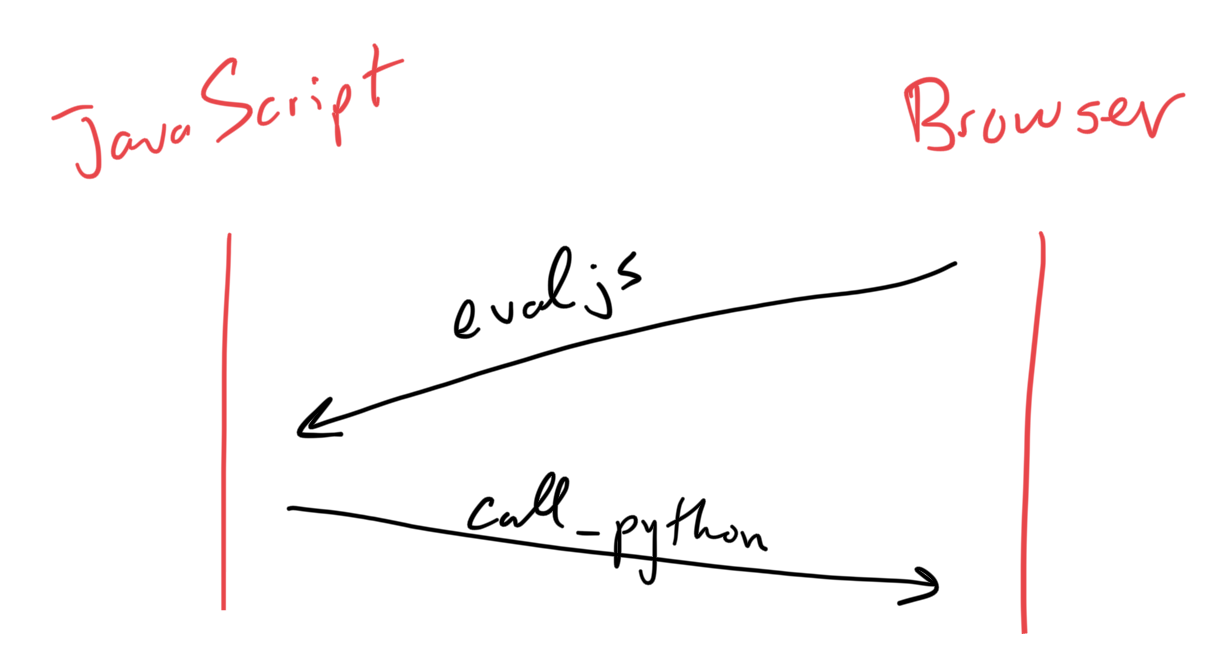
\includegraphics{im/scripts-calls.png}
\caption{The browser can evaluate JavaScript,
  and JavaScript code can call back into the browser.}\label{fig:JavaScript}
\end{figure}

We can call that JavaScript code our ``JavaScript runtime''; we run it
before we run any user code, so let's stick it in a \texttt{runtime.js}
file and execute it when the \texttt{JSContext} is created, before we
run any user code:
\begin{Shaded}
\begin{Highlighting}[]
\NormalTok{RUNTIME\_JS }\OperatorTok{=} \BuiltInTok{open}\NormalTok{(}\StringTok{"runtime.js"}\NormalTok{).read()}

\KeywordTok{class}\NormalTok{ JSContext:}
    \KeywordTok{def} \FunctionTok{\_\_init\_\_}\NormalTok{(}\VariableTok{self}\NormalTok{):}
        \CommentTok{\# ...}
        \VariableTok{self}\NormalTok{.interp.evaljs(RUNTIME\_JS)}
\end{Highlighting}
\end{Shaded}
Now you should be able to put \texttt{console.log("Hi\ from\ JS!")} into
a JavaScript file, run it from your browser, and see output in your
terminal. You should also be able to call \texttt{console.log} multiple
times.

Taking a step back, when we run JavaScript in our browser, we're mixing
C code, which implements the JavaScript interpreter; Python code, which
implements certain JavaScript functions; a JavaScript runtime, which
wraps the Python API to look more like the JavaScript one; and of course
some user code in JavaScript. There's a lot of complexity here!

\begin{bookblock}{further}
If a script runs for a long time, or has an infinite loop, our browser
locks up and becomes completely unresponsive to the user. This is a
consequence of JavaScript's single-threaded semantics and its
task-based,
\href{https://en.wikipedia.org/wiki/Run_to_completion_scheduling}{run-to-completion
scheduling}. Some APIs like
\href{https://developer.mozilla.org/en-US/docs/Web/API/Web_Workers_API}{Web
Workers} allow limited multithreading, but those threads don't have
access to the DOM.
\end{bookblock}

\hypertarget{handling-crashes}{%
\section{Handling Crashes}\label{handling-crashes}}

Crashes in JavaScript code are frustrating to debug. You can cause a
crash by writing bad code, or by explicitly raising an exception, like
so:
\begin{bookblock*}{notcode}
\begin{Shaded}
\begin{Highlighting}[]
\ControlFlowTok{throw} \BuiltInTok{Error}\NormalTok{(}\StringTok{"bad"}\NormalTok{)}\OperatorTok{;}
\end{Highlighting}
\end{Shaded}
\end{bookblock*}
\noindent When a web page runs some JavaScript that crashes, the browser should
ignore the crash. Web pages shouldn't be able to crash our browser! You
can implement that like this:
\begin{Shaded}
\begin{Highlighting}[]
\KeywordTok{class}\NormalTok{ JSContext:}
    \KeywordTok{def}\NormalTok{ run(}\VariableTok{self}\NormalTok{, script, code):}
        \ControlFlowTok{try}\NormalTok{:}
            \ControlFlowTok{return} \VariableTok{self}\NormalTok{.interp.evaljs(code)}
        \ControlFlowTok{except}\NormalTok{ dukpy.JSRuntimeError }\ImportTok{as}\NormalTok{ e:}
            \BuiltInTok{print}\NormalTok{(}\StringTok{"Script"}\NormalTok{, script, }\StringTok{"crashed"}\NormalTok{, e)}
\end{Highlighting}
\end{Shaded}
But as you go through this chapter, you'll also run into another type of
crash: crashes in our own JavaScript runtime. We can't ignore those,
because that's our code. Debugging these crashes is a bear: by default
DukPy won't show a backtrace, and if the runtime code calls into an
exported function that crashes it gets even more confusing.

Here are a few tips to help with these crashes. First, if you get a crash
inside some JavaScript function, wrap the body of the function like
this:
\begin{Shaded}
\begin{Highlighting}[]
\KeywordTok{function} \FunctionTok{foo}\NormalTok{() \{}
    \ControlFlowTok{try}\NormalTok{ \{}
        \CommentTok{// ...}
\NormalTok{    \} }\ControlFlowTok{catch}\NormalTok{(e) \{}
        \BuiltInTok{console}\OperatorTok{.}\FunctionTok{log}\NormalTok{(}\StringTok{"Crash in function foo()"}\OperatorTok{,}\NormalTok{ e}\OperatorTok{.}\AttributeTok{stack}\NormalTok{)}\OperatorTok{;}
        \ControlFlowTok{throw}\NormalTok{ e}\OperatorTok{;}
\NormalTok{    \}}
\NormalTok{\}}
\end{Highlighting}
\end{Shaded}
This code catches all exceptions and prints a stack trace before
re-raising them. If you instead are getting crashes inside an exported
function you will need to wrap that function, on the Python side:
\begin{Shaded}
\begin{Highlighting}[]
\KeywordTok{class}\NormalTok{ JSContext:}
    \KeywordTok{def}\NormalTok{ foo(}\VariableTok{self}\NormalTok{, arg):}
        \ControlFlowTok{try}\NormalTok{:}
            \CommentTok{\# ...}
        \ControlFlowTok{except}\NormalTok{:}
            \ImportTok{import}\NormalTok{ traceback}
\NormalTok{            traceback.print\_exc()}
            \ControlFlowTok{raise}
\end{Highlighting}
\end{Shaded}

Debugging these issues is not easy, because all these calls between
Python and JavaScript get pretty complicated. \emph{Because} these bugs
are hard, it's worth approaching debugging systematically and gathering
a lot of information before attempting a fix.

\hypertarget{returning-handles}{%
\section{Returning Handles}\label{returning-handles}}

So far, JavaScript evaluation is fun but useless, because JavaScript
can't make any kinds of modifications to the page itself. (Why even run
JavaScript if it can't do anything besides print? Who looks at a
browser's console output?) We need to allow JavaScript to modify the
page.

JavaScript manipulates a web page by calling any of a large set of
methods collectively called the DOM API. %, for ``Document Object Model''.
The DOM API is big, and it keeps getting bigger, so we won't be
implementing all, or even most, of it. But a few core functions show key
elements of the full API:
\begin{itemize}
%\tightlist
\item
  \texttt{querySelectorAll} returns all the elements matching a
  selector;
\item
  \texttt{getAttribute} returns an element's value for some attribute;
  and
\item
  \texttt{innerHTML} replaces the contents of an element with new HTML.
\end{itemize}
We'll implement simplified versions of these APIs.\footnote{The
  simplifications will be minor. \texttt{querySelectorAll} will return
  an array, not this thing called a \texttt{NodeList};
  \texttt{innerHTML} will only write the HTML contents of an element,
  and won't allow reading those contents. This suffices to demonstrate
  JavaScript--browser interaction.}

Let's start with \texttt{querySelectorAll}. First, export a function:
\begin{Shaded}
\begin{Highlighting}[]
\KeywordTok{class}\NormalTok{ JSContext:}
    \KeywordTok{def} \FunctionTok{\_\_init\_\_}\NormalTok{(}\VariableTok{self}\NormalTok{):}
        \CommentTok{\# ...}
        \VariableTok{self}\NormalTok{.interp.export\_function(}\StringTok{"querySelectorAll"}\NormalTok{,}
            \VariableTok{self}\NormalTok{.querySelectorAll)}
        \CommentTok{\# ...}
\end{Highlighting}
\end{Shaded}
In JavaScript, \texttt{querySelectorAll} is a method on the
\texttt{document} object, which we need to define in the JavaScript
runtime:
\begin{Shaded}
\begin{Highlighting}[]
\BuiltInTok{document} \OperatorTok{=}\NormalTok{ \{ }\DataTypeTok{querySelectorAll}\OperatorTok{:} \KeywordTok{function}\NormalTok{(s) \{}
    \ControlFlowTok{return} \FunctionTok{call\_python}\NormalTok{(}\StringTok{"querySelectorAll"}\OperatorTok{,}\NormalTok{ s)}\OperatorTok{;}
\NormalTok{\}\}}
\end{Highlighting}
\end{Shaded}
On the Python side, \texttt{querySelectorAll} first has to parse the
selector and then find and return the matching elements. To parse the
selector, I'll call into the \texttt{CSSParser}'s \texttt{selector}
method:\footnote{If you pass \texttt{querySelectorAll} an invalid
  selector, the \texttt{selector} call will throw an error, and DukPy
  will convert that Python-side exception into a JavaScript-side
  exception in the web script we are running, which can catch it.}
\begin{Shaded}
\begin{Highlighting}[]
\KeywordTok{class}\NormalTok{ JSContext:}
    \KeywordTok{def}\NormalTok{ querySelectorAll(}\VariableTok{self}\NormalTok{, selector\_text):}
\NormalTok{        selector }\OperatorTok{=}\NormalTok{ CSSParser(selector\_text).selector()}
\end{Highlighting}
\end{Shaded}

Next we need to find and return all matching elements. To do that, we
need the \texttt{JSContext} to have access to the \texttt{Tab},
specifically to its \texttt{nodes} field. So let's pass in the
\texttt{Tab} when creating a \texttt{JSContext}:
\begin{Shaded}
\begin{Highlighting}[]
\KeywordTok{class}\NormalTok{ JSContext:}
    \KeywordTok{def} \FunctionTok{\_\_init\_\_}\NormalTok{(}\VariableTok{self}\NormalTok{, tab):}
        \VariableTok{self}\NormalTok{.tab }\OperatorTok{=}\NormalTok{ tab}
        \CommentTok{\# ...}

\KeywordTok{class}\NormalTok{ Tab:}
    \KeywordTok{def}\NormalTok{ load(}\VariableTok{self}\NormalTok{, url, payload}\OperatorTok{=}\VariableTok{None}\NormalTok{):}
        \CommentTok{\# ...}
        \VariableTok{self}\NormalTok{.js }\OperatorTok{=}\NormalTok{ JSContext(}\VariableTok{self}\NormalTok{)}
        \CommentTok{\# ...}
\end{Highlighting}
\end{Shaded}
Now \texttt{querySelectorAll} will find all nodes matching the selector:
\begin{Shaded}
\begin{Highlighting}[]
\KeywordTok{def}\NormalTok{ querySelectorAll(}\VariableTok{self}\NormalTok{, selector\_text):}
    \CommentTok{\# ...}
\NormalTok{    nodes }\OperatorTok{=}\NormalTok{ [node }\ControlFlowTok{for}\NormalTok{ node}
             \KeywordTok{in}\NormalTok{ tree\_to\_list(}\VariableTok{self}\NormalTok{.tab.nodes, [])}
             \ControlFlowTok{if}\NormalTok{ selector.matches(node)]}
\end{Highlighting}
\end{Shaded}

Finally, we need to return those nodes back to JavaScript. You might try
something like this:
\begin{Shaded}
\begin{Highlighting}[]
\KeywordTok{def}\NormalTok{ querySelectorAll(}\VariableTok{self}\NormalTok{, selector\_text):}
    \CommentTok{\# ...}
    \ControlFlowTok{return}\NormalTok{ nodes}
\end{Highlighting}
\end{Shaded}
However, this throws an error:\footnote{Yes, that's a confusing error
  message. Is it a \texttt{JSRuntimeError}, an \texttt{EvalError}, or a
  \texttt{TypeError}? The confusion is a consequence of the complex
  interaction of Python, JS, and C code. (JSON, or JavaScript Object Notation,
  is a language-independent data format.)}
\begin{bookblock*}{notcode}
\begin{verbatim}
_dukpy.JSRuntimeError: EvalError:
Error while calling Python Function:
TypeError('Object of type Element is not JSON serializable')
\end{verbatim}
\end{bookblock*}
\noindent What DukPy is trying to tell you is that it has no idea what to do with
the \texttt{Element} objects that \texttt{querySelectorAll} returns.
After all, the \texttt{Element} class only exists in Python, not
JavaScript!

Python objects need to stay on the Python side of the browser, so
JavaScript code will need to refer to them via some kind of indirection.
I'll use simple numeric identifier, which I'll call a
\emph{handle} (see Figure~\ref{fig:Handles}).\footnote{Note the similarity to file descriptors, which
  give user-level applications access to kernel data structures.}

\begin{figure}[b!]
\centering
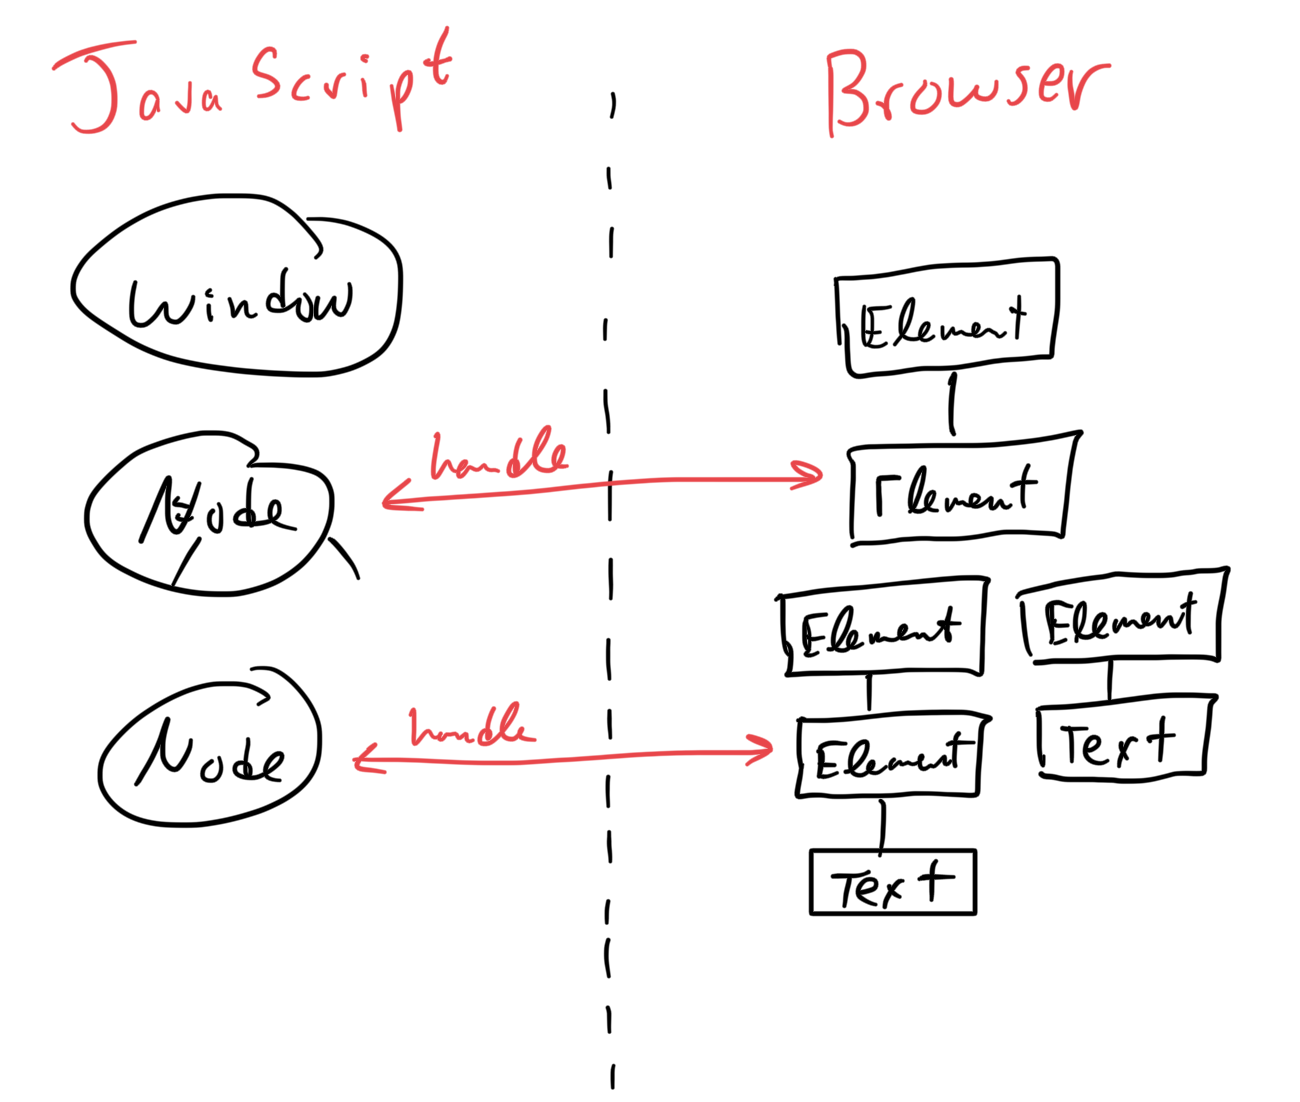
\includegraphics[width=0.8\textwidth]{im/scripts-handles.png}
\caption{The relationship between \texttt{Node} objects in JavaScript
and \texttt{Element}/\texttt{Text} objects in the browser is maintained
through handles.}\label{fig:Handles}
\end{figure}

We'll need to keep track of the handle to node mapping. Let's create a
\texttt{node\_to\_handle} data structure to map nodes to handles, and a
\texttt{handle\_to\_node} map that goes the other way:
\begin{Shaded}
\begin{Highlighting}[]
\KeywordTok{class}\NormalTok{ JSContext:}
    \KeywordTok{def} \FunctionTok{\_\_init\_\_}\NormalTok{(}\VariableTok{self}\NormalTok{, tab):}
        \CommentTok{\# ...}
        \VariableTok{self}\NormalTok{.node\_to\_handle }\OperatorTok{=}\NormalTok{ \{\}}
        \VariableTok{self}\NormalTok{.handle\_to\_node }\OperatorTok{=}\NormalTok{ \{\}}
        \CommentTok{\# ...}
\end{Highlighting}
\end{Shaded}
Now the \texttt{querySelectorAll} handler can allocate handles for each
node and return those handles instead:
\begin{Shaded}
\begin{Highlighting}[]
\KeywordTok{def}\NormalTok{ querySelectorAll(}\VariableTok{self}\NormalTok{, selector\_text):}
    \CommentTok{\# ...}
    \ControlFlowTok{return}\NormalTok{ [}\VariableTok{self}\NormalTok{.get\_handle(node) }\ControlFlowTok{for}\NormalTok{ node }\KeywordTok{in}\NormalTok{ nodes]}
\end{Highlighting}
\end{Shaded}
The \texttt{get\_handle} function should create a new handle if one
doesn't exist yet:
\begin{Shaded}
\begin{Highlighting}[]
\KeywordTok{class}\NormalTok{ JSContext:}
    \KeywordTok{def}\NormalTok{ get\_handle(}\VariableTok{self}\NormalTok{, elt):}
        \ControlFlowTok{if}\NormalTok{ elt }\KeywordTok{not} \KeywordTok{in} \VariableTok{self}\NormalTok{.node\_to\_handle:}
\NormalTok{            handle }\OperatorTok{=} \BuiltInTok{len}\NormalTok{(}\VariableTok{self}\NormalTok{.node\_to\_handle)}
            \VariableTok{self}\NormalTok{.node\_to\_handle[elt] }\OperatorTok{=}\NormalTok{ handle}
            \VariableTok{self}\NormalTok{.handle\_to\_node[handle] }\OperatorTok{=}\NormalTok{ elt}
        \ControlFlowTok{else}\NormalTok{:}
\NormalTok{            handle }\OperatorTok{=} \VariableTok{self}\NormalTok{.node\_to\_handle[elt]}
        \ControlFlowTok{return}\NormalTok{ handle}
\end{Highlighting}
\end{Shaded}

So now the \texttt{querySelectorAll} handler returns something like
\texttt{{[}1,\ 3,\ 4,\ 7{]}}, with each number being a handle for an
element, which DukPy can easily convert into JavaScript objects without
issue. Now of course, on the JavaScript side, \texttt{querySelectorAll}
shouldn't return a bunch of numbers: it should return a list of
\texttt{Node} objects.\footnote{In a real browser,
  \texttt{querySelectorAll} actually returns a
  \href{https://developer.mozilla.org/en-US/docs/Web/API/NodeList}{\texttt{NodeList}
  object}, for kind of abstruse reasons that aren't relevant here.} So
let's define a \texttt{Node} object in our runtime that wraps a
handle:\footnote{If your JavaScript is rusty, you might want to read up
  on the crazy way you define classes in JavaScript. Modern JavaScript
  also provides the \texttt{class} syntax, which is more sensible, but
  it's not supported in DukPy.}
\begin{Shaded}
\begin{Highlighting}[]
\KeywordTok{function} \FunctionTok{Node}\NormalTok{(handle) \{ }\KeywordTok{this}\OperatorTok{.}\AttributeTok{handle} \OperatorTok{=}\NormalTok{ handle}\OperatorTok{;}\NormalTok{ \}}
\end{Highlighting}
\end{Shaded}
We create these \texttt{Node} objects in \texttt{querySelectorAll}'s
wrapper:\footnote{This code creates new \texttt{Node} objects every time
  you call \texttt{querySelectorAll}, even if there's already a
  \texttt{Node} for that handle. That means you can't use equality to
  compare \texttt{Node} objects. I'll ignore that, but a real browser
  wouldn't.}
\begin{Shaded}
\begin{Highlighting}[]
\BuiltInTok{document} \OperatorTok{=}\NormalTok{ \{ }\DataTypeTok{querySelectorAll}\OperatorTok{:} \KeywordTok{function}\NormalTok{(s) \{}
    \KeywordTok{var}\NormalTok{ handles }\OperatorTok{=} \FunctionTok{call\_python}\NormalTok{(}\StringTok{"querySelectorAll"}\OperatorTok{,}\NormalTok{ s)}\OperatorTok{;}
    \ControlFlowTok{return}\NormalTok{ handles}\OperatorTok{.}\FunctionTok{map}\NormalTok{(}\KeywordTok{function}\NormalTok{(h) \{ }\ControlFlowTok{return} \KeywordTok{new} \BuiltInTok{Node}\NormalTok{(h) \})}\OperatorTok{;}
\NormalTok{\}\}}
\end{Highlighting}
\end{Shaded}

\hypertarget{wrapping-handles}{%
\section{Wrapping Handles}\label{wrapping-handles}}

Now that we've got some \texttt{Node}s, what can we do with them?
One simple DOM method is \texttt{getAttribute}, a method on
\texttt{Node} objects that lets you get the value of HTML attributes.
Implementing \texttt{getAttribute} means solving the opposite problem to
\texttt{querySelectorAll}: taking \texttt{Node} objects on the
JavaScript side, and shipping them over to Python.

The solution is similar to \texttt{querySelectorAll}: instead of
shipping the \texttt{Node} object itself, we send over its handle:
\begin{Shaded}
\begin{Highlighting}[]
\BuiltInTok{Node}\OperatorTok{.}\AttributeTok{prototype}\OperatorTok{.}\AttributeTok{getAttribute} \OperatorTok{=} \KeywordTok{function}\NormalTok{(attr) \{}
    \ControlFlowTok{return} \FunctionTok{call\_python}\NormalTok{(}\StringTok{"getAttribute"}\OperatorTok{,} \KeywordTok{this}\OperatorTok{.}\AttributeTok{handle}\OperatorTok{,}\NormalTok{ attr)}\OperatorTok{;}
\NormalTok{\}}
\end{Highlighting}
\end{Shaded}
On the Python side, the \texttt{getAttribute} function takes two
arguments, a handle and an attribute:
\begin{Shaded}
\begin{Highlighting}[]
\KeywordTok{class}\NormalTok{ JSContext:}
    \KeywordTok{def}\NormalTok{ getAttribute(}\VariableTok{self}\NormalTok{, handle, attr):}
\NormalTok{        elt }\OperatorTok{=} \VariableTok{self}\NormalTok{.handle\_to\_node[handle]}
\NormalTok{        attr }\OperatorTok{=}\NormalTok{ elt.attributes.get(attr, }\VariableTok{None}\NormalTok{)}
        \ControlFlowTok{return}\NormalTok{ attr }\ControlFlowTok{if}\NormalTok{ attr }\ControlFlowTok{else} \StringTok{""}
\end{Highlighting}
\end{Shaded}
Note that if the attribute is not assigned, the \texttt{get} method will
return \texttt{None}, which DukPy will translate to JavaScript's
\texttt{null}. Don't forget to export this function as
\texttt{getAttribute}.

We finally have enough of the DOM API to implement a little character
count function for text areas:
\begin{Shaded}
\begin{Highlighting}[]
\NormalTok{inputs }\OperatorTok{=} \BuiltInTok{document}\OperatorTok{.}\FunctionTok{querySelectorAll}\NormalTok{(}\StringTok{\textquotesingle{}input\textquotesingle{}}\NormalTok{)}
\ControlFlowTok{for}\NormalTok{ (}\KeywordTok{var}\NormalTok{ i }\OperatorTok{=} \DecValTok{0}\OperatorTok{;}\NormalTok{ i }\OperatorTok{\textless{}}\NormalTok{ inputs}\OperatorTok{.}\AttributeTok{length}\OperatorTok{;}\NormalTok{ i}\OperatorTok{++}\NormalTok{) \{}
    \KeywordTok{var}\NormalTok{ name }\OperatorTok{=}\NormalTok{ inputs[i]}\OperatorTok{.}\FunctionTok{getAttribute}\NormalTok{(}\StringTok{"name"}\NormalTok{)}\OperatorTok{;}
    \KeywordTok{var}\NormalTok{ value }\OperatorTok{=}\NormalTok{ inputs[i]}\OperatorTok{.}\FunctionTok{getAttribute}\NormalTok{(}\StringTok{"value"}\NormalTok{)}\OperatorTok{;}
    \ControlFlowTok{if}\NormalTok{ (value}\OperatorTok{.}\AttributeTok{length} \OperatorTok{\textgreater{}} \DecValTok{100}\NormalTok{) \{}
        \BuiltInTok{console}\OperatorTok{.}\FunctionTok{log}\NormalTok{(}\StringTok{"Input "} \OperatorTok{+}\NormalTok{ name }\OperatorTok{+} \StringTok{" has too much text."}\NormalTok{)}
\NormalTok{    \}}
\NormalTok{\}}
\end{Highlighting}
\end{Shaded}
Ideally, though, we'd update the character count every time the user
types into an input box, but that requires running JavaScript on every
key press. Let's implement that next.

\begin{bookblock}{further}
\texttt{Node} objects in the DOM correspond to \texttt{Element} nodes in
the browser. They thus have JavaScript object \emph{properties} as well
as HTML \emph{attributes}. They're easy to confuse, and to make matters
worse, many DOM object properties
\href{https://html.spec.whatwg.org/multipage/common-dom-interfaces.html\#reflecting-content-attributes-in-idl-attributes}{\emph{reflect}}
attribute values automatically. For example, the \texttt{id} property on
\texttt{Node} objects gives read-write access to the
\href{https://developer.mozilla.org/en-US/docs/Web/HTML/Global_attributes/id}{\texttt{id}
attribute} of the underlying \texttt{Element}. This is very convenient,
and avoids calling \texttt{setAttribute} and \texttt{getAttribute} all
over the place. But this reflection only applies to certain fields;
setting made-up JavaScript properties won't create corresponding HTML
attributes, nor vice versa.
\end{bookblock}

\hypertarget{event-handling}{%
\section{Event Handling}\label{event-handling}}

The browser executes JavaScript code as soon as it loads the web page,
but that code often wants to change the page \emph{in response} to user
actions.

Here's how that works. Any time the user interacts with the page, the
browser generates \emph{events}.\index{event} Each event has a type,
like \texttt{change}, \texttt{click}, or \texttt{submit}, and happens at
a \emph{target element}. The \texttt{addEventListener} method allows
JavaScript to react to those events:
\texttt{node.addEventListener(\textquotesingle{}click\textquotesingle{},\ func)}
sets \texttt{func} to run every time the element corresponding to
\texttt{node} generates a \texttt{click} event. It's basically Tk's
\texttt{bind}, but in the browser---see Figure~\ref{fig:ScriptEvents}. Let's implement it.

\begin{figure}
\centering
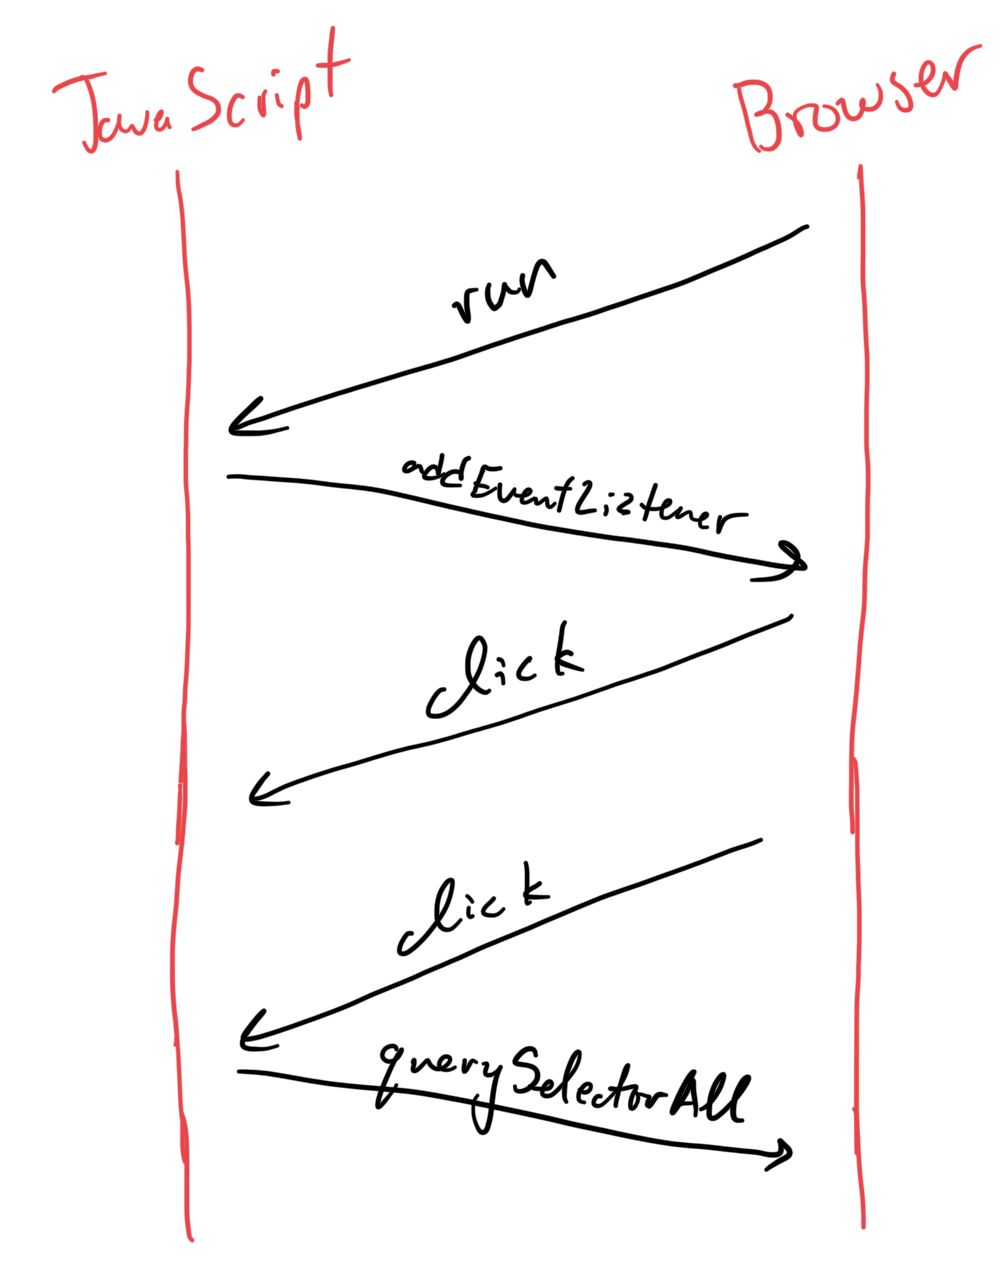
\includegraphics{im/scripts-events.png}
\caption{The browser calls into JavaScript when events happen.}\label{fig:ScriptEvents}
\end{figure}

Let's start with generating events. I'll create a
\texttt{dispatch\_event} method and call it whenever an event is
generated. That includes, first of all, any time we click in the page:
\begin{Shaded}
\begin{Highlighting}[]
\KeywordTok{class}\NormalTok{ Tab:}
    \KeywordTok{def}\NormalTok{ click(}\VariableTok{self}\NormalTok{, x, y):}
        \CommentTok{\# ...}
        \ControlFlowTok{elif}\NormalTok{ elt.tag }\OperatorTok{==} \StringTok{"a"} \KeywordTok{and} \StringTok{"href"} \KeywordTok{in}\NormalTok{ elt.attributes:}
            \VariableTok{self}\NormalTok{.js.dispatch\_event(}\StringTok{"click"}\NormalTok{, elt)}
            \CommentTok{\# ...}
        \ControlFlowTok{elif}\NormalTok{ elt.tag }\OperatorTok{==} \StringTok{"input"}\NormalTok{:}
            \VariableTok{self}\NormalTok{.js.dispatch\_event(}\StringTok{"click"}\NormalTok{, elt)}
            \CommentTok{\# ...}
        \ControlFlowTok{elif}\NormalTok{ elt.tag }\OperatorTok{==} \StringTok{"button"}\NormalTok{:}
            \VariableTok{self}\NormalTok{.js.dispatch\_event(}\StringTok{"click"}\NormalTok{, elt)}
            \CommentTok{\# ...}
        \CommentTok{\# ...}
\end{Highlighting}
\end{Shaded}
Second, before updating input area values:
\begin{Shaded}
\begin{Highlighting}[]
\KeywordTok{class}\NormalTok{ Tab:}
    \KeywordTok{def}\NormalTok{ keypress(}\VariableTok{self}\NormalTok{, char):}
        \ControlFlowTok{if} \VariableTok{self}\NormalTok{.focus:}
            \VariableTok{self}\NormalTok{.js.dispatch\_event(}\StringTok{"keydown"}\NormalTok{, }\VariableTok{self}\NormalTok{.focus)}
            \CommentTok{\# ...}
\end{Highlighting}
\end{Shaded}
And finally, when submitting forms but before actually sending the
request to the server:
\begin{Shaded}
\begin{Highlighting}[]
\KeywordTok{def}\NormalTok{ submit\_form(}\VariableTok{self}\NormalTok{, elt):}
    \VariableTok{self}\NormalTok{.js.dispatch\_event(}\StringTok{"submit"}\NormalTok{, elt)}
    \CommentTok{\# ...}
\end{Highlighting}
\end{Shaded}

So far so good---but what should the \texttt{dispatch\_event} method do?
Well, it needs to run listeners passed to \texttt{addEventListener}, so
those need to be stored somewhere. Since those listeners are JavaScript
functions, we need to keep that data on the JavaScript side, in a
variable in the runtime. I'll call that variable \texttt{LISTENERS};
we'll use it to look up handles and event types, so let's make it map
handles to a dictionary that maps event types to a list of listeners:
\begin{Shaded}
\begin{Highlighting}[]
\NormalTok{LISTENERS }\OperatorTok{=}\NormalTok{ \{\}}

\BuiltInTok{Node}\OperatorTok{.}\AttributeTok{prototype}\OperatorTok{.}\AttributeTok{addEventListener} \OperatorTok{=} \KeywordTok{function}\NormalTok{(type}\OperatorTok{,}\NormalTok{ listener) \{}
    \ControlFlowTok{if}\NormalTok{ (}\OperatorTok{!}\NormalTok{LISTENERS[}\KeywordTok{this}\OperatorTok{.}\AttributeTok{handle}\NormalTok{]) LISTENERS[}\KeywordTok{this}\OperatorTok{.}\AttributeTok{handle}\NormalTok{] }\OperatorTok{=}\NormalTok{ \{\}}\OperatorTok{;}
    \KeywordTok{var}\NormalTok{ dict }\OperatorTok{=}\NormalTok{ LISTENERS[}\KeywordTok{this}\OperatorTok{.}\AttributeTok{handle}\NormalTok{]}\OperatorTok{;}
    \ControlFlowTok{if}\NormalTok{ (}\OperatorTok{!}\NormalTok{dict[type]) dict[type] }\OperatorTok{=}\NormalTok{ []}\OperatorTok{;}
    \KeywordTok{var}\NormalTok{ list }\OperatorTok{=}\NormalTok{ dict[type]}\OperatorTok{;}
\NormalTok{    list}\OperatorTok{.}\FunctionTok{push}\NormalTok{(listener)}\OperatorTok{;}
\NormalTok{\}}
\end{Highlighting}
\end{Shaded}
To dispatch an event, we need to look up the type and handle in the
\texttt{LISTENERS} array, like this:
\begin{Shaded}
\begin{Highlighting}[]
\BuiltInTok{Node}\OperatorTok{.}\AttributeTok{prototype}\OperatorTok{.}\AttributeTok{dispatchEvent} \OperatorTok{=} \KeywordTok{function}\NormalTok{(type) \{}
    \KeywordTok{var}\NormalTok{ handle }\OperatorTok{=} \KeywordTok{this}\OperatorTok{.}\AttributeTok{handle}\OperatorTok{;}
    \KeywordTok{var}\NormalTok{ list }\OperatorTok{=}\NormalTok{ (LISTENERS[handle] }\OperatorTok{\&\&}\NormalTok{ LISTENERS[handle][type]) }\OperatorTok{||}\NormalTok{ []}\OperatorTok{;}
    \ControlFlowTok{for}\NormalTok{ (}\KeywordTok{var}\NormalTok{ i }\OperatorTok{=} \DecValTok{0}\OperatorTok{;}\NormalTok{ i }\OperatorTok{\textless{}}\NormalTok{ list}\OperatorTok{.}\AttributeTok{length}\OperatorTok{;}\NormalTok{ i}\OperatorTok{++}\NormalTok{) \{}
\NormalTok{        list[i]}\OperatorTok{.}\FunctionTok{call}\NormalTok{(}\KeywordTok{this}\NormalTok{)}\OperatorTok{;}
\NormalTok{    \}}
\NormalTok{\}}
\end{Highlighting}
\end{Shaded}
Note that \texttt{dispatchEvent} uses the \texttt{call} method on
functions, which sets the value of \texttt{this} inside that function.
As is standard in JavaScript, I'm setting it to the node that the event
was generated on.

When an event occurs, the browser calls \texttt{dispatchEvent} from
Python:
\begin{Shaded}
\begin{Highlighting}[]
\KeywordTok{class}\NormalTok{ JSContext:}
    \KeywordTok{def}\NormalTok{ dispatch\_event(}\VariableTok{self}\NormalTok{, }\BuiltInTok{type}\NormalTok{, elt):}
\NormalTok{        handle }\OperatorTok{=} \VariableTok{self}\NormalTok{.node\_to\_handle.get(elt, }\OperatorTok{{-}}\DecValTok{1}\NormalTok{)}
        \VariableTok{self}\NormalTok{.interp.evaljs(}
\NormalTok{            EVENT\_DISPATCH\_JS, }\BuiltInTok{type}\OperatorTok{=}\BuiltInTok{type}\NormalTok{, handle}\OperatorTok{=}\NormalTok{handle)}
\end{Highlighting}
\end{Shaded}
Here, the \texttt{EVENT\_DISPATCH\_JS} constant is a string of JavaScript
code that dispatches a new event:
\begin{Shaded}
\begin{Highlighting}[]
\NormalTok{EVENT\_DISPATCH\_JS }\OperatorTok{=} \OperatorTok{\textbackslash{}}
    \StringTok{"new Node(dukpy.handle).dispatchEvent(dukpy.type)"}
\end{Highlighting}
\end{Shaded}
So when \texttt{dispatch\_event} is called on the Python side, that runs
\texttt{dispatchEvent} on the JavaScript side, and that in turn runs all
of the event listeners. The \texttt{dukpy} JavaScript object in this
code snippet stores the named \texttt{type} and \texttt{handle}
arguments to \texttt{evaljs}.

With all this event-handling machinery in place, we can update the
character count every time an input area changes:
\begin{Shaded}
\begin{Highlighting}[]
\KeywordTok{function} \FunctionTok{lengthCheck}\NormalTok{() \{}
    \KeywordTok{var}\NormalTok{ name }\OperatorTok{=} \KeywordTok{this}\OperatorTok{.}\FunctionTok{getAttribute}\NormalTok{(}\StringTok{"name"}\NormalTok{)}\OperatorTok{;}
    \KeywordTok{var}\NormalTok{ value }\OperatorTok{=} \KeywordTok{this}\OperatorTok{.}\FunctionTok{getAttribute}\NormalTok{(}\StringTok{"value"}\NormalTok{)}\OperatorTok{;}
    \ControlFlowTok{if}\NormalTok{ (value}\OperatorTok{.}\AttributeTok{length} \OperatorTok{\textgreater{}} \DecValTok{100}\NormalTok{) \{}
        \BuiltInTok{console}\OperatorTok{.}\FunctionTok{log}\NormalTok{(}\StringTok{"Input "} \OperatorTok{+}\NormalTok{ name }\OperatorTok{+} \StringTok{" has too much text."}\NormalTok{)}
\NormalTok{    \}}
\NormalTok{\}}

\KeywordTok{var}\NormalTok{ inputs }\OperatorTok{=} \BuiltInTok{document}\OperatorTok{.}\FunctionTok{querySelectorAll}\NormalTok{(}\StringTok{"input"}\NormalTok{)}\OperatorTok{;}
\ControlFlowTok{for}\NormalTok{ (}\KeywordTok{var}\NormalTok{ i }\OperatorTok{=} \DecValTok{0}\OperatorTok{;}\NormalTok{ i }\OperatorTok{\textless{}}\NormalTok{ inputs}\OperatorTok{.}\AttributeTok{length}\OperatorTok{;}\NormalTok{ i}\OperatorTok{++}\NormalTok{) \{}
\NormalTok{    inputs[i]}\OperatorTok{.}\FunctionTok{addEventListener}\NormalTok{(}\StringTok{"keydown"}\OperatorTok{,}\NormalTok{ lengthCheck)}\OperatorTok{;}
\NormalTok{\}}
\end{Highlighting}
\end{Shaded}
Note that \texttt{lengthCheck} uses \texttt{this} to reference the input
element that actually changed, as set up by \texttt{dispatchEvent}.

So far so good---but ideally the length check wouldn't print to the
console; it would add a warning to the web page itself. To do that,
we'll need to not only read from the page but also modify it.

\begin{bookblock}{further}
JavaScript
\href{https://auth0.com/blog/a-brief-history-of-javascript/}{first
appeared in 1995}, as part of Netscape Navigator. Its name was chosen to
indicate a similarity to the
\href{https://en.wikipedia.org/wiki/Java_(programming_language)}{Java}
language, and the syntax is Java-esque for that reason. However, under
the surface JavaScript is a much more dynamic language than Java, as is
appropriate given its role as a progressive enhancement mechanism for
the web. For example, any method or property on any object (including
built-in ones like \texttt{Element}) can be dynamically overridden at
any time. This makes it possible to
\href{https://developer.mozilla.org/en-US/docs/Glossary/Polyfill}{polyfill}
differences between browsers, adding features that look built-in to
other JavaScript code.
\end{bookblock}

\hypertarget{modifying-the-dom}{%
\section{Modifying the DOM}\label{modifying-the-dom}}

So far we've implemented read-only DOM methods; now we need methods that
change the page. The full DOM API provides a lot of such methods, but
for simplicity I'm going to implement only \texttt{innerHTML}, which is
used like this:
\begin{bookblock*}{notcode}
\begin{Shaded}
\begin{Highlighting}[]
\NormalTok{node}\OperatorTok{.}\AttributeTok{innerHTML} \OperatorTok{=} \StringTok{"This is my \textless{}b\textgreater{}new\textless{}/b\textgreater{} bit of content!"}\OperatorTok{;}
\end{Highlighting}
\end{Shaded}
\end{bookblock*}
\noindent In other words, \texttt{innerHTML} is a \emph{property} of node objects,
with a \emph{setter} that is run when the field is modified. That setter
takes the new value, which must be a string, parses it as HTML, and
makes the new, parsed HTML nodes children of the original node.

Let's implement this, starting on the JavaScript side. JavaScript has
the obscure \texttt{Object.defineProperty} function to define setters,
which DukPy supports:
\begin{Shaded}
\begin{Highlighting}[]
\BuiltInTok{Object}\OperatorTok{.}\FunctionTok{defineProperty}\NormalTok{(}\BuiltInTok{Node}\OperatorTok{.}\AttributeTok{prototype}\OperatorTok{,} \StringTok{\textquotesingle{}innerHTML\textquotesingle{}}\OperatorTok{,}\NormalTok{ \{}
    \KeywordTok{set}\OperatorTok{:} \KeywordTok{function}\NormalTok{(s) \{}
        \FunctionTok{call\_python}\NormalTok{(}\StringTok{"innerHTML\_set"}\OperatorTok{,} \KeywordTok{this}\OperatorTok{.}\AttributeTok{handle}\OperatorTok{,}\NormalTok{ s}\OperatorTok{.}\FunctionTok{toString}\NormalTok{())}\OperatorTok{;}
\NormalTok{    \}}
\NormalTok{\})}\OperatorTok{;}
\end{Highlighting}
\end{Shaded}
In \texttt{innerHTML\_set}, we'll need to parse the HTML string. That
turns out to be trickier than you'd think, because our browser's HTML
parser is intended to parse whole HTML documents, not these document
fragments. As an expedient, close-enough hack,\footnote{Real browsers
  follow the
  \href{https://html.spec.whatwg.org/\#parsing-html-fragments}{standardized
  parsing algorithm} for HTML fragments.} I'll just wrap the HTML in an
\texttt{html} and \texttt{body} element:
\begin{Shaded}
\begin{Highlighting}[]
\KeywordTok{def}\NormalTok{ innerHTML\_set(}\VariableTok{self}\NormalTok{, handle, s):}
\NormalTok{    doc }\OperatorTok{=}\NormalTok{ HTMLParser(}\StringTok{"\textless{}html\textgreater{}\textless{}body\textgreater{}"} \OperatorTok{+}\NormalTok{ s }\OperatorTok{+} \StringTok{"\textless{}/body\textgreater{}\textless{}/html\textgreater{}"}\NormalTok{).parse()}
\NormalTok{    new\_nodes }\OperatorTok{=}\NormalTok{ doc.children[}\DecValTok{0}\NormalTok{].children}
\end{Highlighting}
\end{Shaded}
Don't forget to export the \texttt{innerHTML\_set} function. Note that
we extract all children of the \texttt{body} element, because an
\texttt{innerHTML\_set} call can create multiple nodes at a time. These
new nodes must now be made children of the element
\texttt{innerHTML\_set} was called on:
\begin{Shaded}
\begin{Highlighting}[]
\KeywordTok{def}\NormalTok{ innerHTML\_set(}\VariableTok{self}\NormalTok{, handle, s):}
    \CommentTok{\# ...}
\NormalTok{    elt }\OperatorTok{=} \VariableTok{self}\NormalTok{.handle\_to\_node[handle]}
\NormalTok{    elt.children }\OperatorTok{=}\NormalTok{ new\_nodes}
    \ControlFlowTok{for}\NormalTok{ child }\KeywordTok{in}\NormalTok{ elt.children:}
\NormalTok{        child.parent }\OperatorTok{=}\NormalTok{ elt}
\end{Highlighting}
\end{Shaded}
We update the parent pointers of those parsed child nodes because
otherwise they would point to the dummy \texttt{body} element that we
added to aid parsing.

It might look like we're done---but try this out and you'll realize that
nothing happens when a script calls \texttt{innerHTML\_set}. That's
because, while we have changed the HTML tree, we haven't regenerated the
layout tree or the display list, so the browser is still showing the old
page.

Whenever the page changes, we need to update its rendering by calling
\texttt{render}:\footnote{Redoing layout for the whole page is often
  wasteful; % \href{invalidation.md}{Chapter 16}
  Chapter~\ref{ch:PreviousComputations} explores a more
  complicated algorithm that speeds this up.}
\begin{Shaded}
\begin{Highlighting}[]
\KeywordTok{class}\NormalTok{ JSContext:}
    \KeywordTok{def}\NormalTok{ innerHTML\_set(}\VariableTok{self}\NormalTok{, handle, s):}
        \CommentTok{\# ...}
        \VariableTok{self}\NormalTok{.tab.render()}
\end{Highlighting}
\end{Shaded}
JavaScript can now modify the web page!\footnote{Note that while
  rendering will update to account for the new HTML, any added scripts
  or style sheets will not properly load, and removed style sheets will
  (incorrectly) still apply. I've left fixing that % to an exercise
  as Exercise~\ref{ex:AddedScripts}.}

Let's try this out in our guest book. Say we want a 100-character limit
on guest book entries to prevent long, incoherent rants from making it
in.
First, switch to the server codebase and add a
\texttt{\textless{}strong\textgreater{}} after the guest book form.
Initially this element will be empty, but we'll write an error message
into it if the paragraph gets too long.
\begin{Shaded}
\begin{Highlighting}[]
\KeywordTok{def}\NormalTok{ show\_comments():}
    \CommentTok{\# ...}
\NormalTok{    out }\OperatorTok{+=} \StringTok{"\textless{}strong\textgreater{}\textless{}/strong\textgreater{}"}
    \CommentTok{\# ...}
\end{Highlighting}
\end{Shaded}
Also add a script to the page.
\begin{Shaded}
\begin{Highlighting}[]
\KeywordTok{def}\NormalTok{ show\_comments():}
    \CommentTok{\# ...}
\NormalTok{    out }\OperatorTok{+=} \StringTok{"\textless{}script src=/comment.js\textgreater{}\textless{}/script\textgreater{}"}
    \CommentTok{\# ...}
\end{Highlighting}
\end{Shaded}
Now the browser will request \texttt{comment.js}, so our server needs to
\emph{serve} that JavaScript file:
\begin{Shaded}
\begin{Highlighting}[]
\KeywordTok{def}\NormalTok{ do\_request(method, url, headers, body):}
    \CommentTok{\# ...}
    \ControlFlowTok{elif}\NormalTok{ method }\OperatorTok{==} \StringTok{"GET"} \KeywordTok{and}\NormalTok{ url }\OperatorTok{==} \StringTok{"/comment.js"}\NormalTok{:}
        \ControlFlowTok{with} \BuiltInTok{open}\NormalTok{(}\StringTok{"comment.js"}\NormalTok{) }\ImportTok{as}\NormalTok{ f:}
            \ControlFlowTok{return} \StringTok{"200 OK"}\NormalTok{, f.read()}
    \CommentTok{\# ...}
\end{Highlighting}
\end{Shaded}
We can then put our little input length checker into
\texttt{comment.js}, with the \texttt{lengthCheck} function modified to
use \texttt{innerHTML}:
\begin{Shaded}
\begin{Highlighting}[]
\KeywordTok{var}\NormalTok{ strong }\OperatorTok{=} \BuiltInTok{document}\OperatorTok{.}\FunctionTok{querySelectorAll}\NormalTok{(}\StringTok{"strong"}\NormalTok{)[}\DecValTok{0}\NormalTok{]}\OperatorTok{;}

\KeywordTok{function} \FunctionTok{lengthCheck}\NormalTok{() \{}
    \KeywordTok{var}\NormalTok{ value }\OperatorTok{=} \KeywordTok{this}\OperatorTok{.}\FunctionTok{getAttribute}\NormalTok{(}\StringTok{"value"}\NormalTok{)}\OperatorTok{;}
    \ControlFlowTok{if}\NormalTok{ (value}\OperatorTok{.}\AttributeTok{length} \OperatorTok{\textgreater{}} \DecValTok{100}\NormalTok{) \{}
\NormalTok{        strong}\OperatorTok{.}\AttributeTok{innerHTML} \OperatorTok{=} \StringTok{"Comment too long!"}\OperatorTok{;}
\NormalTok{    \}}
\NormalTok{\}}

\KeywordTok{var}\NormalTok{ inputs }\OperatorTok{=} \BuiltInTok{document}\OperatorTok{.}\FunctionTok{querySelectorAll}\NormalTok{(}\StringTok{"input"}\NormalTok{)}\OperatorTok{;}
\ControlFlowTok{for}\NormalTok{ (}\KeywordTok{var}\NormalTok{ i }\OperatorTok{=} \DecValTok{0}\OperatorTok{;}\NormalTok{ i }\OperatorTok{\textless{}}\NormalTok{ inputs}\OperatorTok{.}\AttributeTok{length}\OperatorTok{;}\NormalTok{ i}\OperatorTok{++}\NormalTok{) \{}
\NormalTok{    inputs[i]}\OperatorTok{.}\FunctionTok{addEventListener}\NormalTok{(}\StringTok{"keydown"}\OperatorTok{,}\NormalTok{ lengthCheck)}\OperatorTok{;}
\NormalTok{\}}
\end{Highlighting}
\end{Shaded}

Try it out: write a long comment and you should see the page warning you
% that the comment is
when it grows too long. By the way, we might want to make it stand
out more, so let's go ahead and add another URL to our web server,
\texttt{/comment.css}, with the contents:
\begin{Shaded}
\begin{Highlighting}[]
\NormalTok{strong \{ }\KeywordTok{font{-}weight}\CharTok{:} \DecValTok{bold}\OperatorTok{;} \KeywordTok{color}\CharTok{:} \ConstantTok{red}\OperatorTok{;}\NormalTok{ \}}
\end{Highlighting}
\end{Shaded}
Add a \texttt{link} to the guest book page so that this style sheet is
loaded.

But even though we tell the user that their comment is too long, the user
can submit the guest book entry anyway. Oops! Let's fix that.

\begin{bookblock}{further}
This code has a subtle memory leak: if you access an HTML element from
JavaScript (thereby creating a handle for it) and then remove the
element from the page (using \texttt{innerHTML}), Python won't be able
to garbage-collect the \texttt{Element} object because it is still
stored in the \texttt{node\_to\_handle} map. And that's good, if
JavaScript can still access that \texttt{Element} via its handle, but
bad otherwise. Solving this is quite tricky, because it requires the
Python and JavaScript garbage collectors to
\href{https://research.google/pubs/pub47359/}{cooperate}.
\end{bookblock}

\hypertarget{event-defaults}{%
\section{Event Defaults}\label{event-defaults}}

So far, when an event is generated, the browser will run the listeners,
and then \emph{also} do whatever it normally does for that event---the
\emph{default action}. I'd now like JavaScript code to be able to
\emph{cancel} that default action.
There are a few steps involved. First of all, event listeners should
receive an \emph{event object} as an argument. That object should have a
\texttt{preventDefault} method. When that method is called, the default
action shouldn't occur.

First of all, we'll need event objects. Back to our JavaScript runtime:
\begin{Shaded}
\begin{Highlighting}[]
\KeywordTok{function} \FunctionTok{Event}\NormalTok{(type) \{}
    \KeywordTok{this}\OperatorTok{.}\AttributeTok{type} \OperatorTok{=}\NormalTok{ type}
    \KeywordTok{this}\OperatorTok{.}\AttributeTok{do\_default} \OperatorTok{=} \KeywordTok{true}\OperatorTok{;}
\NormalTok{\}}

\BuiltInTok{Event}\OperatorTok{.}\AttributeTok{prototype}\OperatorTok{.}\AttributeTok{preventDefault} \OperatorTok{=} \KeywordTok{function}\NormalTok{() \{}
    \KeywordTok{this}\OperatorTok{.}\AttributeTok{do\_default} \OperatorTok{=} \KeywordTok{false}\OperatorTok{;}
\NormalTok{\}}
\end{Highlighting}
\end{Shaded}
Note the \texttt{do\_default} field, to record whether
\texttt{preventDefault} has been called. We'll now be passing an
\texttt{Event} object to \texttt{dispatchEvent}, instead of just the
event type:
\begin{Shaded}
\begin{Highlighting}[]
\BuiltInTok{Node}\OperatorTok{.}\AttributeTok{prototype}\OperatorTok{.}\AttributeTok{dispatchEvent} \OperatorTok{=} \KeywordTok{function}\NormalTok{(evt) \{}
    \KeywordTok{var}\NormalTok{ type }\OperatorTok{=}\NormalTok{ evt}\OperatorTok{.}\AttributeTok{type}\OperatorTok{;}
    \CommentTok{// ...}
    \ControlFlowTok{for}\NormalTok{ (}\KeywordTok{var}\NormalTok{ i }\OperatorTok{=} \DecValTok{0}\OperatorTok{;}\NormalTok{ i }\OperatorTok{\textless{}}\NormalTok{ list}\OperatorTok{.}\AttributeTok{length}\OperatorTok{;}\NormalTok{ i}\OperatorTok{++}\NormalTok{) \{}
\NormalTok{        list[i]}\OperatorTok{.}\FunctionTok{call}\NormalTok{(}\KeywordTok{this}\OperatorTok{,}\NormalTok{ evt)}\OperatorTok{;}
\NormalTok{    \}}
    \CommentTok{// ...}
    \ControlFlowTok{return}\NormalTok{ evt}\OperatorTok{.}\AttributeTok{do\_default}\OperatorTok{;}
\NormalTok{\}}
\end{Highlighting}
\end{Shaded}

In Python, we now need to create an \texttt{Event} to pass to
\texttt{dispatchEvent}:
\begin{Shaded}
\begin{Highlighting}[]
\NormalTok{EVENT\_DISPATCH\_JS }\OperatorTok{=} \OperatorTok{\textbackslash{}}
    \StringTok{"new Node(dukpy.handle).dispatchEvent(new Event(dukpy.type))"}
\end{Highlighting}
\end{Shaded}
Also note that \texttt{dispatchEvent} returns \texttt{evt.do\_default},
which is not only standard in JavaScript but also helpful when
dispatching events from Python, because Python's
\texttt{dispatch\_event} can return that boolean to its handler:
\begin{Shaded}
\begin{Highlighting}[]
\KeywordTok{class}\NormalTok{ JSContext:}
    \KeywordTok{def}\NormalTok{ dispatch\_event(}\VariableTok{self}\NormalTok{, }\BuiltInTok{type}\NormalTok{, elt):}
        \CommentTok{\# ...}
\NormalTok{        do\_default }\OperatorTok{=} \VariableTok{self}\NormalTok{.interp.evaljs(}
\NormalTok{            EVENT\_DISPATCH\_JS, }\BuiltInTok{type}\OperatorTok{=}\BuiltInTok{type}\NormalTok{, handle}\OperatorTok{=}\NormalTok{handle)}
        \ControlFlowTok{return} \KeywordTok{not}\NormalTok{ do\_default}
\end{Highlighting}
\end{Shaded}
This way, every time an event happens, the browser can check the return
value of \texttt{dispatch\_event} and stop if it is \texttt{True}. We
have three such places in the \texttt{click} method:
\begin{Shaded}
\begin{Highlighting}[]
\KeywordTok{class}\NormalTok{ Tab:}
    \KeywordTok{def}\NormalTok{ click(}\VariableTok{self}\NormalTok{, x, y):}
        \ControlFlowTok{while}\NormalTok{ elt:}
            \CommentTok{\# ...}
            \ControlFlowTok{elif}\NormalTok{ elt.tag }\OperatorTok{==} \StringTok{"a"} \KeywordTok{and} \StringTok{"href"} \KeywordTok{in}\NormalTok{ elt.attributes:}
                \ControlFlowTok{if} \VariableTok{self}\NormalTok{.js.dispatch\_event(}\StringTok{"click"}\NormalTok{, elt): }\ControlFlowTok{return}
                \CommentTok{\# ...}
            \ControlFlowTok{elif}\NormalTok{ elt.tag }\OperatorTok{==} \StringTok{"input"}\NormalTok{:}
                \ControlFlowTok{if} \VariableTok{self}\NormalTok{.js.dispatch\_event(}\StringTok{"click"}\NormalTok{, elt): }\ControlFlowTok{return}
                \CommentTok{\# ...}
            \ControlFlowTok{elif}\NormalTok{ elt.tag }\OperatorTok{==} \StringTok{"button"}\NormalTok{:}
                \ControlFlowTok{if} \VariableTok{self}\NormalTok{.js.dispatch\_event(}\StringTok{"click"}\NormalTok{, elt): }\ControlFlowTok{return}
                \CommentTok{\# ...}
            \CommentTok{\# ...}
         \CommentTok{\# ...}
\end{Highlighting}
\end{Shaded}
And one in \texttt{submit\_form}:
\begin{Shaded}
\begin{Highlighting}[]
\KeywordTok{class}\NormalTok{ Tab:}
    \KeywordTok{def}\NormalTok{ submit\_form(}\VariableTok{self}\NormalTok{, elt):}
        \ControlFlowTok{if} \VariableTok{self}\NormalTok{.js.dispatch\_event(}\StringTok{"submit"}\NormalTok{, elt): }\ControlFlowTok{return}
\end{Highlighting}
\end{Shaded}
And one in \texttt{keypress}:
\begin{Shaded}
\begin{Highlighting}[]
\KeywordTok{class}\NormalTok{ Tab:}
    \KeywordTok{def}\NormalTok{ keypress(}\VariableTok{self}\NormalTok{, char):}
        \ControlFlowTok{if} \VariableTok{self}\NormalTok{.focus:}
            \ControlFlowTok{if} \VariableTok{self}\NormalTok{.js.dispatch\_event(}\StringTok{"keydown"}\NormalTok{, }\VariableTok{self}\NormalTok{.focus): }\ControlFlowTok{return}
\end{Highlighting}
\end{Shaded}

Now our character count code can prevent the user from submitting a
form: it can use a global variable to track whether or not submission is
allowed, and then when submission is attempted it can check that
variable and cancel that submission if necessary:
\begin{Shaded}
\begin{Highlighting}[]
\KeywordTok{var}\NormalTok{ allow\_submit }\OperatorTok{=} \KeywordTok{true}\OperatorTok{;}

\KeywordTok{function} \FunctionTok{lengthCheck}\NormalTok{() \{}
    \CommentTok{// ...}
\NormalTok{    allow\_submit }\OperatorTok{=}\NormalTok{ value}\OperatorTok{.}\AttributeTok{length} \OperatorTok{\textless{}=} \DecValTok{100}\OperatorTok{;}
    \ControlFlowTok{if}\NormalTok{ (}\OperatorTok{!}\NormalTok{allow\_submit) \{}
        \CommentTok{// ...}
\NormalTok{    \}}
\NormalTok{\}}

\KeywordTok{var}\NormalTok{ form }\OperatorTok{=} \BuiltInTok{document}\OperatorTok{.}\FunctionTok{querySelectorAll}\NormalTok{(}\StringTok{"form"}\NormalTok{)[}\DecValTok{0}\NormalTok{]}\OperatorTok{;}
\NormalTok{form}\OperatorTok{.}\FunctionTok{addEventListener}\NormalTok{(}\StringTok{"submit"}\OperatorTok{,} \KeywordTok{function}\NormalTok{(e) \{}
    \ControlFlowTok{if}\NormalTok{ (}\OperatorTok{!}\NormalTok{allow\_submit) e}\OperatorTok{.}\FunctionTok{preventDefault}\NormalTok{()}\OperatorTok{;}
\NormalTok{\})}\OperatorTok{;}
\end{Highlighting}
\end{Shaded}
This way it's impossible to submit the form when the comment is too
long!

Well\ \ldots\ impossible in this browser. But since there are browsers
that don't run JavaScript (like ours, one chapter back), we should check
the length on the server side too:
\begin{Shaded}
\begin{Highlighting}[]
\KeywordTok{def}\NormalTok{ add\_entry(params):}
    \ControlFlowTok{if} \StringTok{\textquotesingle{}guest\textquotesingle{}} \KeywordTok{in}\NormalTok{ params }\KeywordTok{and} \BuiltInTok{len}\NormalTok{(params[}\StringTok{\textquotesingle{}guest\textquotesingle{}}\NormalTok{]) }\OperatorTok{\textless{}=} \DecValTok{100}\NormalTok{:}
\NormalTok{        ENTRIES.append(params[}\StringTok{\textquotesingle{}guest\textquotesingle{}}\NormalTok{])}
    \ControlFlowTok{return}\NormalTok{ show\_comments()}
\end{Highlighting}
\end{Shaded}
Note that we shouldn't---can't---rely on JavaScript being executed by
the browser, because the browser is the user's agent, not ours. Ideally,
web pages should be written so that they work correctly without
JavaScript, but work better with it. This is called
\href{https://en.wikipedia.org/wiki/Progressive_enhancement}{progressive
enhancement}, and it means we're not replicating in JavaScript what the
browser can already do.

A closing thought: while our guest book now has a little bit of
JavaScript code, it's still mostly HTML, CSS, form elements, other
standard web features. In this way JavaScript extends the web instead of
replacing it. This is in contrast to the recently departed
\href{https://www.adobe.com/products/flashplayer/end-of-life.html}{Adobe
Flash}, and before that
\href{https://en.wikipedia.org/wiki/Java_applet}{Java Applets}, which
were self-contained plug-ins that handled input and rendering on their
own.

\begin{bookblock}{further}
Search engines are constantly
\href{https://en.wikipedia.org/wiki/Web_crawler}{crawling} the web and
\href{https://en.wikipedia.org/wiki/Search_engine_indexing}{indexing}
all of the web pages they can find. In the early days, indexing was just
a matter of loading the HTML, parsing it, and extracting the information.
But these days, a lot of
\href{https://en.wikipedia.org/wiki/Single-page_application}{single-page
app} sites use JavaScript to
\href{https://en.wikipedia.org/wiki/Hydration_(web_development)}{``hydrate''}\footnotemark\ their
site into its full
contents. On such sites, before hydration happens, the information in
the site is hidden inside of JavaScript data structures. For this
reason, search engines need to not just parse HTML, but also run
JavaScript (and load style sheets) during indexing. In other words, the
indexing systems use browsers (such as, for example,
\href{https://chromium.googlesource.com/chromium/src/+/lkgr/headless/README.md}{headless
Chrome})---one more place browsers appear in the web ecosystem.
\end{bookblock}
\footnotetext{
This
  process is called ``hydration'' by analogy with how water is added to
  dehydrated food to make it edible again.}

\hypertarget{summary}{%
\section{Summary}\label{Scripts-summary}}

Our browser now runs JavaScript applications on behalf of websites.
Granted, it supports just four methods from the vast DOM API, but even
those demonstrate:
\begin{itemize}
% \tightlist
\item
  generating handles to allow scripts to refer to page elements;
\item
  reading attribute values from page elements;
\item
  writing and modifying page elements;
\item
  attaching event listeners so that scripts can respond to page events.
\end{itemize}
A web page can now add functionality via a clever script, instead of
waiting for a browser developer to add it into the browser itself. And
as a side benefit, a web page can now earn the lofty title of ``web
application''.

\hypertarget{outline}{%
\section{Outline}\label{Scripts-outline}}

The complete set of functions, classes, and methods in our browser
should now look something like this:
\begin{Shaded}
\begin{Highlighting}[]
\NormalTok{WIDTH}
\NormalTok{HEIGHT}
\NormalTok{HSTEP}
\NormalTok{VSTEP}
\NormalTok{SCROLL\_STEP}
\NormalTok{FONTS}
\KeywordTok{def}\NormalTok{ get\_font(size, weight, slant)}
\KeywordTok{def}\NormalTok{ print\_tree(node, indent)}
\KeywordTok{class}\NormalTok{ HTMLParser:}
    \KeywordTok{def} \FunctionTok{\_\_init\_\_}\NormalTok{(body)}
    \KeywordTok{def}\NormalTok{ parse()}
    \KeywordTok{def}\NormalTok{ get\_attributes(text)}
    \KeywordTok{def}\NormalTok{ add\_text(text)}
\NormalTok{    SELF\_CLOSING\_TAGS}
    \KeywordTok{def}\NormalTok{ add\_tag(tag)}
\NormalTok{    HEAD\_TAGS}
    \KeywordTok{def}\NormalTok{ implicit\_tags(tag)}
    \KeywordTok{def}\NormalTok{ finish()}
\NormalTok{BLOCK\_ELEMENTS}
\KeywordTok{class}\NormalTok{ CSSParser:}
    \KeywordTok{def} \FunctionTok{\_\_init\_\_}\NormalTok{(s)}
    \KeywordTok{def}\NormalTok{ whitespace()}
    \KeywordTok{def}\NormalTok{ literal(literal)}
    \KeywordTok{def}\NormalTok{ word()}
    \KeywordTok{def}\NormalTok{ pair()}
    \KeywordTok{def}\NormalTok{ ignore\_until(chars)}
    \KeywordTok{def}\NormalTok{ body()}
    \KeywordTok{def}\NormalTok{ selector()}
    \KeywordTok{def}\NormalTok{ parse()}
\KeywordTok{class}\NormalTok{ TagSelector:}
    \KeywordTok{def} \FunctionTok{\_\_init\_\_}\NormalTok{(tag)}
    \KeywordTok{def}\NormalTok{ matches(node)}
\KeywordTok{class}\NormalTok{ DescendantSelector:}
    \KeywordTok{def} \FunctionTok{\_\_init\_\_}\NormalTok{(ancestor, descendant)}
    \KeywordTok{def}\NormalTok{ matches(node)}
\NormalTok{INHERITED\_PROPERTIES}
\KeywordTok{def}\NormalTok{ style(node, rules)}
\KeywordTok{def}\NormalTok{ cascade\_priority(rule)}
\KeywordTok{class}\NormalTok{ DrawText:}
    \KeywordTok{def} \FunctionTok{\_\_init\_\_}\NormalTok{(x1, y1, text, font, color)}
    \KeywordTok{def}\NormalTok{ execute(scroll, canvas)}
\KeywordTok{def}\NormalTok{ tree\_to\_list(tree, }\NormalTok{list}\NormalTok{)}
\KeywordTok{class}\NormalTok{ DrawLine:}
    \KeywordTok{def} \FunctionTok{\_\_init\_\_}\NormalTok{(x1, y1, x2, y2, color, thickness)}
    \KeywordTok{def}\NormalTok{ execute(scroll, canvas)}
\KeywordTok{class}\NormalTok{ DrawOutline:}
    \KeywordTok{def} \FunctionTok{\_\_init\_\_}\NormalTok{(rect, color, thickness)}
    \KeywordTok{def}\NormalTok{ execute(scroll, canvas)}
\KeywordTok{class}\NormalTok{ DrawRect:}
    \KeywordTok{def} \FunctionTok{\_\_init\_\_}\NormalTok{(rect, color)}
    \KeywordTok{def}\NormalTok{ execute(scroll, canvas)}
\KeywordTok{class}\NormalTok{ URL:}
    \KeywordTok{def} \FunctionTok{\_\_init\_\_}\NormalTok{(url)}
    \KeywordTok{def}\NormalTok{ request(payload)}
    \KeywordTok{def}\NormalTok{ resolve(url)}
\KeywordTok{class}\NormalTok{ Element:}
    \KeywordTok{def} \FunctionTok{\_\_init\_\_}\NormalTok{(tag, attributes, parent)}
    \KeywordTok{def} \FunctionTok{\_\_repr\_\_}\NormalTok{()}
\KeywordTok{class}\NormalTok{ Text:}
    \KeywordTok{def} \FunctionTok{\_\_init\_\_}\NormalTok{(text, parent)}
    \KeywordTok{def} \FunctionTok{\_\_repr\_\_}\NormalTok{()}
\KeywordTok{class}\NormalTok{ Browser:}
    \KeywordTok{def} \FunctionTok{\_\_init\_\_}\NormalTok{()}
    \KeywordTok{def}\NormalTok{ handle\_down(e)}
    \KeywordTok{def}\NormalTok{ handle\_click(e)}
    \KeywordTok{def}\NormalTok{ handle\_key(e)}
    \KeywordTok{def}\NormalTok{ handle\_enter(e)}
    \KeywordTok{def}\NormalTok{ new\_tab(url)}
    \KeywordTok{def}\NormalTok{ draw()}
\KeywordTok{class}\NormalTok{ Tab:}
    \KeywordTok{def} \FunctionTok{\_\_init\_\_}\NormalTok{(tab\_height)}
    \KeywordTok{def}\NormalTok{ load(url, payload)}
    \KeywordTok{def}\NormalTok{ draw(canvas, offset)}
    \KeywordTok{def}\NormalTok{ scrolldown()}
    \KeywordTok{def}\NormalTok{ click(x, y)}
    \KeywordTok{def}\NormalTok{ go\_back()}
    \KeywordTok{def}\NormalTok{ render()}
    \KeywordTok{def}\NormalTok{ submit\_form(elt)}
    \KeywordTok{def}\NormalTok{ keypress(char)}
\KeywordTok{class}\NormalTok{ DocumentLayout:}
    \KeywordTok{def} \FunctionTok{\_\_init\_\_}\NormalTok{(node)}
    \KeywordTok{def}\NormalTok{ layout()}
    \KeywordTok{def}\NormalTok{ paint()}
    \KeywordTok{def}\NormalTok{ should\_paint()}
\KeywordTok{class}\NormalTok{ BlockLayout:}
    \KeywordTok{def} \FunctionTok{\_\_init\_\_}\NormalTok{(node, parent, previous)}
    \KeywordTok{def}\NormalTok{ token(tok)}
    \KeywordTok{def}\NormalTok{ word(node, word)}
    \KeywordTok{def}\NormalTok{ flush()}
    \KeywordTok{def}\NormalTok{ recurse(node)}
    \KeywordTok{def}\NormalTok{ layout()}
    \KeywordTok{def}\NormalTok{ layout\_mode()}
    \KeywordTok{def}\NormalTok{ paint()}
    \KeywordTok{def}\NormalTok{ new\_line()}
    \KeywordTok{def}\NormalTok{ self\_rect()}
    \KeywordTok{def} \NormalTok{input}\NormalTok{(node)}
    \KeywordTok{def}\NormalTok{ should\_paint()}
\KeywordTok{class}\NormalTok{ InputLayout:}
    \KeywordTok{def} \FunctionTok{\_\_init\_\_}\NormalTok{(node, parent, previous)}
    \KeywordTok{def}\NormalTok{ layout()}
    \KeywordTok{def}\NormalTok{ should\_paint()}
    \KeywordTok{def}\NormalTok{ self\_rect()}
    \KeywordTok{def}\NormalTok{ paint()}
\NormalTok{DEFAULT\_STYLE\_SHEET}
\NormalTok{INPUT\_WIDTH\_PX}
\KeywordTok{class}\NormalTok{ LineLayout:}
    \KeywordTok{def} \FunctionTok{\_\_init\_\_}\NormalTok{(node, parent, previous)}
    \KeywordTok{def}\NormalTok{ layout()}
    \KeywordTok{def}\NormalTok{ paint()}
    \KeywordTok{def}\NormalTok{ should\_paint()}
\KeywordTok{class}\NormalTok{ TextLayout:}
    \KeywordTok{def} \FunctionTok{\_\_init\_\_}\NormalTok{(node, word, parent, previous)}
    \KeywordTok{def}\NormalTok{ layout()}
    \KeywordTok{def}\NormalTok{ paint()}
    \KeywordTok{def}\NormalTok{ should\_paint()}
\NormalTok{EVENT\_DISPATCH\_JS}
\NormalTok{RUNTIME\_JS}
\KeywordTok{class}\NormalTok{ JSContext:}
    \KeywordTok{def} \FunctionTok{\_\_init\_\_}\NormalTok{(tab)}
    \KeywordTok{def}\NormalTok{ run(code)}
    \KeywordTok{def}\NormalTok{ dispatch\_event(}\NormalTok{type}\NormalTok{, elt)}
    \KeywordTok{def}\NormalTok{ get\_handle(elt)}
    \KeywordTok{def}\NormalTok{ querySelectorAll(selector\_text)}
    \KeywordTok{def}\NormalTok{ getAttribute(handle, attr)}
    \KeywordTok{def}\NormalTok{ innerHTML\_set(handle, s)}
\end{Highlighting}
\end{Shaded}

\hypertarget{exercises}{%
\section{Exercises}\label{Scripts-exercises}}
\begin{enumerate}[label=\thechapter-\arabic*]
\item \emph{\texttt{Node.children}.} Add support for the
\href{https://developer.mozilla.org/en-US/docs/Web/API/Element/children}{\texttt{children}}
property on JavaScript \texttt{Node}s. \texttt{Node.children} returns
the immediate \texttt{Element} children of a node, as an array.
\texttt{Text} children are not included.\footnote{The DOM method
  \texttt{childNodes} gives access to both elements and text.}

\item\label{ex:CreateElement} \emph{\texttt{createElement}.} The
\href{https://developer.mozilla.org/en-US/docs/Web/API/Document/createElement}{\texttt{document.createElement}}
method creates a new element, which can be \emph{attached} to the
document with the
\href{https://developer.mozilla.org/en-US/docs/Web/API/Node/appendChild}{\texttt{appendChild}}
and
\href{https://developer.mozilla.org/en-US/docs/Web/API/Node/insertBefore}{\texttt{insertBefore}}
methods on \texttt{Node}s; unlike \texttt{innerHTML}, there's no parsing
involved. Implement all three methods.

\item\label{ex:RemoveChild} \emph{\texttt{removeChild}.} The
\href{https://developer.mozilla.org/en-US/docs/Web/API/Node/removeChild}{\texttt{removeChild}}
method on \texttt{Node}s detaches the provided child and returns it,
bringing that child---and its subtree---back into a \emph{detached}
state. (It can then be \emph{re-attached} elsewhere, with
\texttt{appendChild} and \texttt{insertBefore}, or deleted.) Implement
this method. It's more challenging to implement this one, because you'll
need to also remove the subtree from the Python side.

\item \emph{IDs.} When an HTML element has an \texttt{id} attribute, a
JavaScript variable pointing to that element is predefined. So, if a
page has a
\texttt{\textless{}div\ id="foo"\textgreater{}\textless{}/div\textgreater{}},
then there's a variable \texttt{foo} referring to that node.\footnote{This
  is
  \href{http://www.whatwg.org/specs/web-apps/current-work/\#named-access-on-the-window-object}{standard}
  behavior.} Implement this in your browser. Make sure to handle the
case of nodes being added and removed (such as with \texttt{innerHTML}).

\item \emph{Event bubbling.} Right now, you can attach a \texttt{click}
handler to \texttt{a} (anchor) elements, but not to anything else. Fix
this. One challenge you'll face is that when you click on an element,
you also click on all its ancestors. On the web, this sort of quirk is
handled by
\href{https://developer.mozilla.org/en-US/docs/Learn/JavaScript/Building_blocks/Events\#event_bubbling}{\emph{event
bubbling}}: when an event is generated on an element, listeners are run
not just on that element but also on its ancestors. Implement event
bubbling, and make sure listeners can call \texttt{stopPropagation} on
the event object to stop bubbling the event up the tree. Double-check
that clicking on links still works, and make sure
\texttt{preventDefault} still successfully prevents clicks on a link
from actually following the link.

\item \emph{Serializing HTML.} Reading from
\href{https://developer.mozilla.org/en-US/docs/Web/API/Element/innerHTML}{\texttt{innerHTML}}
should return a string containing HTML source code. That source code
should reflect the \emph{current} attributes of the element; for
example:
\begin{bookblock*}{notcode}
\begin{Shaded}
\begin{Highlighting}[]
\NormalTok{element}\OperatorTok{.}\AttributeTok{innerHTML} \OperatorTok{=} \StringTok{\textquotesingle{}\textless{}span id=foo\textgreater{}Chris was here\textless{}/span\textgreater{}\textquotesingle{}}\OperatorTok{;}
\NormalTok{element}\OperatorTok{.}\AttributeTok{id} \OperatorTok{=} \StringTok{\textquotesingle{}bar\textquotesingle{}}\OperatorTok{;}
\CommentTok{// Prints "\textless{}span id=bar\textgreater{}Chris was here\textless{}/span\textgreater{}":}
\BuiltInTok{console}\OperatorTok{.}\FunctionTok{log}\NormalTok{(element}\OperatorTok{.}\AttributeTok{innerHTML}\NormalTok{)}\OperatorTok{;}
\end{Highlighting}
\end{Shaded}
\end{bookblock*}
\noindent Implement this behavior for \texttt{innerHTML} as a getter. Also
implement \texttt{outerHTML}, which differs from \texttt{innerHTML} in
that it contains the element itself, not just its children.

\item\label{ex:AddedScripts} \emph{Script-added scripts and style sheets.} The \texttt{innerHTML} API
could cause \texttt{\textless{}script\textgreater{}} or
\texttt{\textless{}link\textgreater{}} elements to be added to the
document, but currently our browser does not load them when this
happens. Fix this. Likewise, when a
\texttt{\textless{}link\textgreater{}} element is removed from the
document, its style sheet should be removed from the global list;
implement that as well.\footnote{Note that, unlike a style sheet, a
  removed \texttt{\textless{}script\textgreater{}}'s evaluated code
  still exists for the lifetime of the web page. Can you see why it has
  to be that way?}
\end{enumerate}

\ifprintedoutput
\theendnotes
\setcounter{endnote}{0}
\fi

\chapter{Keeping Data Private}\label{ch:KeepingDataPrivate}
Our browser has grown up and now runs (small) web applications. With one
final step---user identity via cookies---it will be able to run all
sorts of personalized online services. But capability demands
responsibility: our browser must now secure cookies against adversaries
interested in stealing them. Luckily, browsers have sophisticated
systems for controlling access to cookies and preventing their misuse.

\begin{bookblock}{warning}
Web security\index{web!security} is a vast topic, covering browser,
network, and applications security. It also involves educating the user,
so that attackers can't mislead them into revealing their own secure
data. This chapter can't cover all of that: if you're writing web
applications or other security-sensitive code, this book is not enough.
\end{bookblock}

\hypertarget{cookies}{%
\section{Cookies}\label{cookies}}

With what we've implemented so far, there's no way for a web server to
tell whether two HTTP requests come from the same user or from two
different ones; our browser is effectively anonymous.\footnote{I don't
  mean anonymous against malicious attackers, who might use
  \emph{browser fingerprinting} or similar techniques to tell users
  apart. I mean anonymous in the good-faith sense.} That means it can't
``log in'' anywhere, since a logged-in user's requests would be
indistinguishable from those of not-logged-in users.

The web fixes this problem with cookies\index{cookie}. A cookie---the
name is meaningless, ignore it---is a little bit of information stored
by your browser on behalf of a web server. The cookie distinguishes your
browser from any other, and is sent with each web request so the server
can distinguish which requests come from whom. In effect, a cookie is a
decentralized, server-granted identity for your browser.

Here are the technical details. An HTTP response can contain a
\texttt{Set-Cookie} header. This header contains a key--value pair; for
example, the following header sets the value of the \texttt{foo} cookie
to \texttt{bar}:
\begin{bookblock*}{notcode}
\begin{verbatim}
Set-Cookie: foo=bar
\end{verbatim}
\end{bookblock*}
\noindent The browser remembers this key--value pair, and the next time it makes a
request to the same server (cookies are site-specific), the browser
echoes it back in the \texttt{Cookie} header:
\begin{bookblock*}{notcode}
\begin{verbatim}
Cookie: foo=bar
\end{verbatim}
\end{bookblock*}

Servers can
set multiple cookies, and also set parameters like
expiration dates, but this \texttt{Set-Cookie}/\texttt{Cookie}
% mechanism
transaction as shown in Figure~\ref{fig:Cookies} is the core principle.

\begin{figure}[b!]
\centering
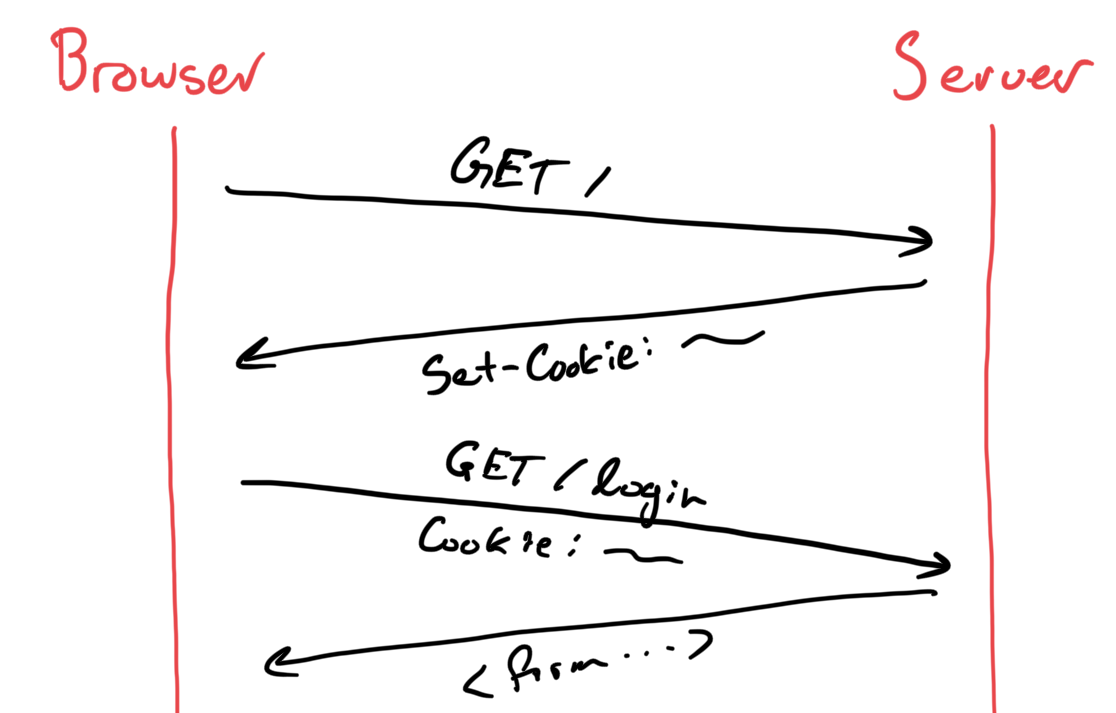
\includegraphics{im/security-cookies.png}
\caption{The server assigns cookies to the browser with the
\texttt{Set-Cookie} header, and the browser thereafter identifies itself
with the \texttt{Cookie} header.}\label{fig:Cookies}
\end{figure}

Let's use cookies to write a login system for our guest book. Each user
will be identified by a long random number stored in the \texttt{token}
cookie.\footnote{This \texttt{random.random} call returns a decimal
  number with 53 bits of randomness. That's not great; 256 bits is
  typically the goal. And \texttt{random.random} is not a secure random
  number generator: by observing enough tokens you can predict future
  values and use those to hijack accounts. A real web application must
  use a cryptographically secure random number generator for tokens.}
The server will either extract a token from the \texttt{Cookie} header,
or generate a new one for new visitors:
\begin{Shaded}
\begin{Highlighting}[]
\ImportTok{import}\NormalTok{ random}

\KeywordTok{def}\NormalTok{ handle\_connection(conx):}
    \CommentTok{\# ...}
    \ControlFlowTok{if} \StringTok{"cookie"} \KeywordTok{in}\NormalTok{ headers:}
\NormalTok{        token }\OperatorTok{=}\NormalTok{ headers[}\StringTok{"cookie"}\NormalTok{][}\BuiltInTok{len}\NormalTok{(}\StringTok{"token="}\NormalTok{):]}
    \ControlFlowTok{else}\NormalTok{:}
\NormalTok{        token }\OperatorTok{=} \BuiltInTok{str}\NormalTok{(random.random())[}\DecValTok{2}\NormalTok{:]}
    \CommentTok{\# ...}
\end{Highlighting}
\end{Shaded}
Of course, new visitors need to be told to remember their
newly generated token:
\begin{Shaded}
\begin{Highlighting}[]
\KeywordTok{def}\NormalTok{ handle\_connection(conx):}
    \CommentTok{\# ...}
    \ControlFlowTok{if} \StringTok{\textquotesingle{}cookie\textquotesingle{}} \KeywordTok{not} \KeywordTok{in}\NormalTok{ headers:}
\NormalTok{        template }\OperatorTok{=} \StringTok{"Set{-}Cookie: token=}\SpecialCharTok{\{\}}\CharTok{\textbackslash{}r\textbackslash{}n}\StringTok{"}
\NormalTok{        response }\OperatorTok{+=}\NormalTok{ template.}\BuiltInTok{format}\NormalTok{(token)}
    \CommentTok{\# ...}
\end{Highlighting}
\end{Shaded}
The first code block runs after all the request headers are parsed,
before handling the request in \texttt{do\_request}, while the second
code block runs after \texttt{do\_request} returns, when the server is
assembling the HTTP response.

With these two code changes, each visitor to the guest book now has a
unique identity. We can now use that identity to store information about
each user. Let's do that in a server side \texttt{SESSIONS}
variable:\footnote{Browsers and servers both limit header lengths, so
  it's best to store minimal data in cookies. Plus, cookies are sent
  back and forth on every request, so long cookies mean a lot of useless
  traffic. It's therefore wise to store user data on the server, and
  only store a pointer to that data in the cookie. And, since cookies
  are stored by the browser, they can be changed arbitrarily by the
  user, so it would be insecure to trust the cookie data.}
\begin{Shaded}
\begin{Highlighting}[]
\NormalTok{SESSIONS }\OperatorTok{=}\NormalTok{ \{\}}

\KeywordTok{def}\NormalTok{ handle\_connection(conx):}
    \CommentTok{\# ...}
\NormalTok{    session }\OperatorTok{=}\NormalTok{ SESSIONS.setdefault(token, \{\})}
\NormalTok{    status, body }\OperatorTok{=}\NormalTok{ do\_request(session, method, url, headers, body)}
    \CommentTok{\# ...}
\end{Highlighting}
\end{Shaded}
\texttt{SESSIONS} maps tokens to session data dictionaries. The
\texttt{setdefault} method both gets a key from a dictionary and also
sets a default value if the key isn't present. I'm passing that session
data via \texttt{do\_request} to individual pages like
\texttt{show\_comments} and \texttt{add\_entry}:
\begin{Shaded}
\begin{Highlighting}[]
\KeywordTok{def}\NormalTok{ do\_request(session, method, url, headers, body):}
    \ControlFlowTok{if}\NormalTok{ method }\OperatorTok{==} \StringTok{"GET"} \KeywordTok{and}\NormalTok{ url }\OperatorTok{==} \StringTok{"/"}\NormalTok{:}
        \ControlFlowTok{return} \StringTok{"200 OK"}\NormalTok{, show\_comments(session)}
    \CommentTok{\# ...}
    \ControlFlowTok{elif}\NormalTok{ method }\OperatorTok{==} \StringTok{"POST"} \KeywordTok{and}\NormalTok{ url }\OperatorTok{==} \StringTok{"/add"}\NormalTok{:}
\NormalTok{        params }\OperatorTok{=}\NormalTok{ form\_decode(body)}
\NormalTok{        add\_entry(session, params)}
        \ControlFlowTok{return} \StringTok{"200 OK"}\NormalTok{, show\_comments(session)}
    \CommentTok{\# ...}
\end{Highlighting}
\end{Shaded}
You'll need to modify the argument lists for \texttt{add\_entry} and
\texttt{show\_comments} to accept this new argument. We now have the
foundation upon which to build a login system.

\begin{bookblock}{further}
The \href{https://curl.se/rfc/cookie_spec.html}{original specification}
for cookies says there is ``no compelling reason'' for calling them
``cookies'', but in fact using this term for opaque identifiers
exchanged between programs seems to date way back;
\href{https://en.wikipedia.org/wiki/Magic_cookie}{Wikipedia} traces it
back to at least 1979, and cookies were used in
\href{https://en.wikipedia.org/wiki/X_Window_authorization\#Cookie-based_access}{X11}
for authentication before they were used on the web.
\end{bookblock}

\hypertarget{a-login-system}{%
\section{A Login System}\label{a-login-system}}

I want users to log in before posting to the guest book. Minimally, that
means:
\begin{itemize}
%\tightlist
\item
  Users will log in with a username and password.
\item
  The server will check if the login is valid.
\item
  Users have to be logged in to add guest book entries.
\item
  The server will display who added which guest book entry.
\end{itemize}

Let's start coding. We'll hard-code two user/password pairs:
\begin{Shaded}
\begin{Highlighting}[]
\NormalTok{LOGINS }\OperatorTok{=}\NormalTok{ \{}
    \StringTok{"crashoverride"}\NormalTok{: }\StringTok{"0cool"}\NormalTok{,}
    \StringTok{"cerealkiller"}\NormalTok{: }\StringTok{"emmanuel"}
\NormalTok{\}}
\end{Highlighting}
\end{Shaded}
Users will log in by going to \texttt{/login}:
\begin{Shaded}
\begin{Highlighting}[]
\KeywordTok{def}\NormalTok{ do\_request(session, method, url, headers, body):}
    \CommentTok{\# ...}
    \ControlFlowTok{elif}\NormalTok{ method }\OperatorTok{==} \StringTok{"GET"} \KeywordTok{and}\NormalTok{ url }\OperatorTok{==} \StringTok{"/login"}\NormalTok{:}
        \ControlFlowTok{return} \StringTok{"200 OK"}\NormalTok{, login\_form(session)}
    \CommentTok{\# ...}
\end{Highlighting}
\end{Shaded}
This page shows a form with a username and a password
field:\footnote{I've given the \texttt{password} input area the type
  \texttt{password}, which in a real browser will draw stars or dots
  instead of showing what you've entered, though our browser doesn't do
  that. % }\footnote{
  Also, do note that this is not particularly accessible HTML,
  lacking, for example, \texttt{\textless{}label\textgreater{}} elements
  around the form labels. Not that our browser supports that!}
\begin{Shaded}
\begin{Highlighting}[]
\KeywordTok{def}\NormalTok{ login\_form(session):}
\NormalTok{    body }\OperatorTok{=} \StringTok{"\textless{}!doctype html\textgreater{}"}
\NormalTok{    body }\OperatorTok{+=} \StringTok{"\textless{}form action=/ method=post\textgreater{}"}
\NormalTok{    body }\OperatorTok{+=} \StringTok{"\textless{}p\textgreater{}Username: \textless{}input name=username\textgreater{}\textless{}/p\textgreater{}"}
\NormalTok{    body }\OperatorTok{+=} \StringTok{"\textless{}p\textgreater{}Password: \textless{}input name=password type=password\textgreater{}\textless{}/p\textgreater{}"}
\NormalTok{    body }\OperatorTok{+=} \StringTok{"\textless{}p\textgreater{}\textless{}button\textgreater{}Log in\textless{}/button\textgreater{}\textless{}/p\textgreater{}"}
\NormalTok{    body }\OperatorTok{+=} \StringTok{"\textless{}/form\textgreater{}"}
    \ControlFlowTok{return}\NormalTok{ body }
\end{Highlighting}
\end{Shaded}

Note that the form \texttt{POST}s its data to the \texttt{/} URL. We'll
want to handle these \texttt{POST} requests in a new function that
checks passwords and does logins:
\begin{Shaded}
\begin{Highlighting}[]
\KeywordTok{def}\NormalTok{ do\_request(session, method, url, headers, body):}
    \CommentTok{\# ...}
    \ControlFlowTok{elif}\NormalTok{ method }\OperatorTok{==} \StringTok{"POST"} \KeywordTok{and}\NormalTok{ url }\OperatorTok{==} \StringTok{"/"}\NormalTok{:}
\NormalTok{        params }\OperatorTok{=}\NormalTok{ form\_decode(body)}
        \ControlFlowTok{return}\NormalTok{ do\_login(session, params)}
    \CommentTok{\# ...}
\end{Highlighting}
\end{Shaded}
This \texttt{do\_login} function checks passwords and logs people in by
storing their user name in the session data:\footnote{Actually, using
  \texttt{==} to compare passwords like this is a bad idea: Python's
  equality function for strings scans the string from left to right, and
  exits as soon as it finds a difference. Therefore, you get a clue
  about the password from \emph{how long} it takes to check a password
  guess; this is called a
  \href{https://en.wikipedia.org/wiki/Timing_attack}{timing side
  channel}. This book is about the browser, not the server, but a real
  web application has to do a
  \href{https://www.chosenplaintext.ca/articles/beginners-guide-constant-time-cryptography.html}{constant-time
  string comparison}!}
\begin{Shaded}
\begin{Highlighting}[]
\KeywordTok{def}\NormalTok{ do\_login(session, params):}
\NormalTok{    username }\OperatorTok{=}\NormalTok{ params.get(}\StringTok{"username"}\NormalTok{)}
\NormalTok{    password }\OperatorTok{=}\NormalTok{ params.get(}\StringTok{"password"}\NormalTok{)}
    \ControlFlowTok{if}\NormalTok{ username }\KeywordTok{in}\NormalTok{ LOGINS }\KeywordTok{and}\NormalTok{ LOGINS[username] }\OperatorTok{==}\NormalTok{ password:}
\NormalTok{        session[}\StringTok{"user"}\NormalTok{] }\OperatorTok{=}\NormalTok{ username}
        \ControlFlowTok{return} \StringTok{"200 OK"}\NormalTok{, show\_comments(session)}
    \ControlFlowTok{else}\NormalTok{:}
\NormalTok{        out }\OperatorTok{=} \StringTok{"\textless{}!doctype html\textgreater{}"}
\NormalTok{        out }\OperatorTok{+=} \StringTok{"\textless{}h1\textgreater{}Invalid password for }\SpecialCharTok{\{\}}\StringTok{\textless{}/h1\textgreater{}"}\NormalTok{.}\BuiltInTok{format}\NormalTok{(username)}
        \ControlFlowTok{return} \StringTok{"401 Unauthorized"}\NormalTok{, out}
\end{Highlighting}
\end{Shaded}

Note that the session data (including the \texttt{user} key) is stored
on the server, so users can't modify it directly. That's good, because
we only want to set the \texttt{user} key in the session data if users
supply the right password in the login form.

So now we can check if a user is logged in by checking the
\texttt{session} data. Let's only show the comment form to logged in
users:
\begin{Shaded}
\begin{Highlighting}[]
\KeywordTok{def}\NormalTok{ show\_comments(session):}
    \CommentTok{\# ...}
    \ControlFlowTok{if} \StringTok{"user"} \KeywordTok{in}\NormalTok{ session:}
\NormalTok{        out }\OperatorTok{+=} \StringTok{"\textless{}h1\textgreater{}Hello, "} \OperatorTok{+}\NormalTok{ session[}\StringTok{"user"}\NormalTok{] }\OperatorTok{+} \StringTok{"\textless{}/h1\textgreater{}"}
\NormalTok{        out }\OperatorTok{+=} \StringTok{"\textless{}form action=add method=post\textgreater{}"}
\NormalTok{        out }\OperatorTok{+=}   \StringTok{"\textless{}p\textgreater{}\textless{}input name=guest\textgreater{}\textless{}/p\textgreater{}"}
\NormalTok{        out }\OperatorTok{+=}   \StringTok{"\textless{}p\textgreater{}\textless{}button\textgreater{}Sign the book!\textless{}/button\textgreater{}\textless{}/p\textgreater{}"}
\NormalTok{        out }\OperatorTok{+=} \StringTok{"\textless{}/form\textgreater{}"}
    \ControlFlowTok{else}\NormalTok{:}
\NormalTok{        out }\OperatorTok{+=} \StringTok{"\textless{}a href=/login\textgreater{}Sign in to write in the guest book\textless{}/a\textgreater{}"}
    \CommentTok{\# ...}
\end{Highlighting}
\end{Shaded}
Likewise, \texttt{add\_entry} must check that the user is logged in
before posting comments:
\begin{Shaded}
\begin{Highlighting}[]
\KeywordTok{def}\NormalTok{ add\_entry(session, params):}
    \ControlFlowTok{if} \StringTok{"user"} \KeywordTok{not} \KeywordTok{in}\NormalTok{ session: }\ControlFlowTok{return}
    \ControlFlowTok{if} \StringTok{\textquotesingle{}guest\textquotesingle{}} \KeywordTok{in}\NormalTok{ params }\KeywordTok{and} \BuiltInTok{len}\NormalTok{(params[}\StringTok{\textquotesingle{}guest\textquotesingle{}}\NormalTok{]) }\OperatorTok{\textless{}=} \DecValTok{100}\NormalTok{:}
\NormalTok{        ENTRIES.append((params[}\StringTok{\textquotesingle{}guest\textquotesingle{}}\NormalTok{], session[}\StringTok{"user"}\NormalTok{]))}
\end{Highlighting}
\end{Shaded}
Note that the username from the session is stored into
\texttt{ENTRIES}:\footnote{The pre-loaded comments reference 1995's
  \emph{Hackers}. \href{https://xkcd.com/1337}{Hack the Planet!}}
\begin{Shaded}
\begin{Highlighting}[]
\NormalTok{ENTRIES }\OperatorTok{=}\NormalTok{ [}
\NormalTok{    (}\StringTok{"No names. We are nameless!"}\NormalTok{, }\StringTok{"cerealkiller"}\NormalTok{),}
\NormalTok{    (}\StringTok{"HACK THE PLANET!!!"}\NormalTok{, }\StringTok{"crashoverride"}\NormalTok{),}
\NormalTok{]}
\end{Highlighting}
\end{Shaded}
When we print the guest book entries, we'll show who authored them:
\begin{Shaded}
\begin{Highlighting}[]
\KeywordTok{def}\NormalTok{ show\_comments(session):}
    \CommentTok{\# ...}
    \ControlFlowTok{for}\NormalTok{ entry, who }\KeywordTok{in}\NormalTok{ ENTRIES:}
\NormalTok{        out }\OperatorTok{+=} \StringTok{"\textless{}p\textgreater{}"} \OperatorTok{+}\NormalTok{ entry }\OperatorTok{+} \StringTok{"}\CharTok{\textbackslash{}n}\StringTok{"}
\NormalTok{        out }\OperatorTok{+=} \StringTok{"\textless{}i\textgreater{}by "} \OperatorTok{+}\NormalTok{ who }\OperatorTok{+} \StringTok{"\textless{}/i\textgreater{}\textless{}/p\textgreater{}"}
    \CommentTok{\# ...}
\end{Highlighting}
\end{Shaded}

Try it out in a normal web browser. You should be able to go to the main
guest book page, click the link to log in, log in with one of the
username--password pairs above, and then be able to post
entries.\footnote{The login flow slows down debugging. You might want to
  add the empty string as a username--password pair.} Of course, this
login system has a whole slew of insecurities.\footnote{The insecurities
  include not hashing passwords, not using
  \href{https://auth0.com/blog/hashing-in-action-understanding-bcrypt/}{\texttt{bcrypt}},
  not allowing password changes, not having a ``forget your password''
  flow, not forcing TLS, not sandboxing the server, and many, many
  others.} But the focus of this book is the browser, not the server, so
once you're sure it's all working, let's switch back to our web browser
and implement cookies.

\begin{bookblock}{further}
A more obscure browser authentication system is
\href{https://aboutssl.org/ssl-tls-client-authentication-how-does-it-works/}{TLS
client certificates}. The user downloads a public/private key pair from
the server, and the browser then uses them to prove who it is on later
requests to that server. Also, if you've ever seen a URL with
\texttt{username:password@} before the hostname, that's
\href{https://developer.mozilla.org/en-US/docs/Web/HTTP/Authentication}{HTTP
authentication}. Please don't use either method in new websites (without
a good reason).
\end{bookblock}

\hypertarget{implementing-cookies}{%
\section{Implementing Cookies}\label{implementing-cookies}}

To start, we need a place in the browser that stores cookies; that data
structure is traditionally called a \emph{cookie jar}:\footnote{Because
  once you have one silly name it's important to stay on-brand.}
\begin{Shaded}
\begin{Highlighting}[]
\NormalTok{COOKIE\_JAR }\OperatorTok{=}\NormalTok{ \{\}}
\end{Highlighting}
\end{Shaded}
Since cookies are site-specific, our cookie jar will map sites to
cookies. Note that the cookie jar is global, not limited to a particular
tab. That means that if you're logged in to a website and you open a
second tab, you're logged in on that tab as well.\footnote{Moreover,
  since \texttt{request} can be called multiple times on one page---to
  load CSS and JavaScript---later requests transmit cookies set by
  previous responses. For example, our guest book sets a cookie when the
  browser first requests the page and then receives that cookie when our
  browser later requests the page's CSS file.}

When the browser visits a page, it needs to send the cookie for that
site:
\begin{Shaded}
\begin{Highlighting}[]
\KeywordTok{class}\NormalTok{ URL:}
    \KeywordTok{def}\NormalTok{ request(}\VariableTok{self}\NormalTok{, payload}\OperatorTok{=}\VariableTok{None}\NormalTok{):}
        \CommentTok{\# ...}
        \ControlFlowTok{if} \VariableTok{self}\NormalTok{.host }\KeywordTok{in}\NormalTok{ COOKIE\_JAR:}
\NormalTok{            cookie }\OperatorTok{=}\NormalTok{ COOKIE\_JAR[}\VariableTok{self}\NormalTok{.host]}
\NormalTok{            request }\OperatorTok{+=} \StringTok{"Cookie: }\SpecialCharTok{\{\}}\CharTok{\textbackslash{}r\textbackslash{}n}\StringTok{"}\NormalTok{.}\BuiltInTok{format}\NormalTok{(cookie)}
        \CommentTok{\# ...}
\end{Highlighting}
\end{Shaded}
Symmetrically, the browser has to update the cookie jar when it sees a
\texttt{Set-Cookie} header:\footnote{A server can actually send multiple
  \texttt{Set-Cookie} headers to set multiple cookies in one request,
  though our browser won't handle that correctly.}
\begin{Shaded}
\begin{Highlighting}[]
\KeywordTok{class}\NormalTok{ URL:}
    \KeywordTok{def}\NormalTok{ request(}\VariableTok{self}\NormalTok{, payload}\OperatorTok{=}\VariableTok{None}\NormalTok{):}
        \CommentTok{\# ...}
        \ControlFlowTok{if} \StringTok{"set{-}cookie"} \KeywordTok{in}\NormalTok{ response\_headers:}
\NormalTok{            cookie }\OperatorTok{=}\NormalTok{ response\_headers[}\StringTok{"set{-}cookie"}\NormalTok{]}
\NormalTok{            COOKIE\_JAR[}\VariableTok{self}\NormalTok{.host] }\OperatorTok{=}\NormalTok{ cookie}
        \CommentTok{\# ...}
\end{Highlighting}
\end{Shaded}

You should now be able to use your browser to log in to the guest book
and post to it. Moreover, you should be able to open the guest book in
two browsers simultaneously---maybe your browser and a real browser as
well---and log in and post as two different users.

Now that our browser supports cookies and uses them for logins, we need
to make sure cookie data is safe from malicious actors. After all, the
cookie is the browser's identity, so if someone stole it, the server
would think they are you. We need to prevent that.

\begin{bookblock}{further}
At one point, an attempt was made to ``clean up'' the cookie
specification in
\href{https://datatracker.ietf.org/doc/html/rfc2965}{RFC~2965},
including human-readable cookie descriptions and cookies restricted to
certain ports. This required introducing the \texttt{Cookie2} and
\texttt{Set-Cookie2} headers; the new headers were not popular. They are
now \href{https://datatracker.ietf.org/doc/html/rfc6265}{obsolete}.
\end{bookblock}

\hypertarget{cross-site-requests}{%
\section{Cross-Site Requests}\label{cross-site-requests}}

Cookies are site-specific, so one server shouldn't be sent another
server's cookies.\footnote{Well \ldots\ Our connection isn't encrypted,
  so an attacker could read it from an open Wi-Fi connection. But another
  \emph{server} couldn't. % }\footnote{Well\ldots{}
  Or how about this attack: another server could
  hijack our DNS and redirect our hostname to a different IP address,
  and then steal our cookies. Some % ISPs
  internet service providers support DNSSEC, which prevents
  this, but not all. % }\footnote{Well\ldots{}
  Or consider this attack: a state-level attacker could
  announce fradulent BGP (Border Gateway Protocol) routes, which would send even a
  correctly retrieved IP address to the wrong physical computer. % }\footnote{
  (Security is very hard.)} But if an attacker is clever, they might be able to get
\emph{the server} or \emph{the browser} to help them steal cookie
values.

The easiest way for an attacker to steal your private data is to ask for
it. Of course, there's no API in the browser for a website to ask for
another website's cookies. But there \emph{is} an API to make requests
to another website. It's called \texttt{XMLHttpRequest}.\footnote{It's a
  weird name! Why is \texttt{XML} capitalized but not \texttt{Http}? And
  it's not restricted to XML! Ultimately, the naming is
  \href{https://en.wikipedia.org/wiki/XMLHttpRequest\#History}{historical},
  dating back to Microsoft's ``Outlook Web Access'' feature for Exchange
  Server 2000.}
\texttt{XMLHttpRequest} sends asynchronous HTTP requests from
JavaScript. Since I'm using \texttt{XMLHttpRequest} just to illustrate
security issues, I'll implement a minimal version here. Specifically,
I'll support only \emph{synchronous} requests.\footnote{Synchronous
  \texttt{XMLHttpRequest}s are slowly moving through
  \href{https://xhr.spec.whatwg.org/\#the-open()-method}{deprecation and
  obsolescence}, but I'm using them here because they are easier to
  implement.} Using this minimal \texttt{XMLHttpRequest} looks like
this:
\begin{bookblock*}{notcode}
\begin{Shaded}
\begin{Highlighting}[]
\NormalTok{x }\OperatorTok{=} \KeywordTok{new} \BuiltInTok{XMLHttpRequest}\NormalTok{()}\OperatorTok{;}
\NormalTok{x}\OperatorTok{.}\FunctionTok{open}\NormalTok{(}\StringTok{"GET"}\OperatorTok{,}\NormalTok{ url}\OperatorTok{,} \KeywordTok{false}\NormalTok{)}\OperatorTok{;}
\NormalTok{x}\OperatorTok{.}\FunctionTok{send}\NormalTok{()}\OperatorTok{;}
\CommentTok{// use x.responseText}
\end{Highlighting}
\end{Shaded}
\end{bookblock*}

We'll define the \texttt{XMLHttpRequest} objects and methods in
JavaScript. The \texttt{open} method will just save the method and
URL:\footnote{\texttt{XMLHttpRequest} has more options not implemented
  here, like support for usernames and passwords. This code is also
  missing some error checking, like making sure the method is a valid
  HTTP method supported by our browser.}
\begin{Shaded}
\begin{Highlighting}[]
\KeywordTok{function} \FunctionTok{XMLHttpRequest}\NormalTok{() \{\}}

\BuiltInTok{XMLHttpRequest}\OperatorTok{.}\AttributeTok{prototype}\OperatorTok{.}\AttributeTok{open} \OperatorTok{=} \KeywordTok{function}\NormalTok{(method}\OperatorTok{,}\NormalTok{ url}\OperatorTok{,}\NormalTok{ is\_async) \{}
    \ControlFlowTok{if}\NormalTok{ (is\_async) }\ControlFlowTok{throw} \BuiltInTok{Error}\NormalTok{(}\StringTok{"Asynchronous XHR is not supported"}\NormalTok{)}\OperatorTok{;}
    \KeywordTok{this}\OperatorTok{.}\AttributeTok{method} \OperatorTok{=}\NormalTok{ method}\OperatorTok{;}
    \KeywordTok{this}\OperatorTok{.}\AttributeTok{url} \OperatorTok{=}\NormalTok{ url}\OperatorTok{;}
\NormalTok{\}}
\end{Highlighting}
\end{Shaded}
The \texttt{send} method calls an exported function:\footnote{As above,
  this implementation skips important \texttt{XMLHttpRequest} features,
  like setting request headers (and reading response headers), changing
  the response type, or triggering various events and callbacks during
  the request.}
\begin{Shaded}
\begin{Highlighting}[]
\BuiltInTok{XMLHttpRequest}\OperatorTok{.}\AttributeTok{prototype}\OperatorTok{.}\AttributeTok{send} \OperatorTok{=} \KeywordTok{function}\NormalTok{(body) \{}
    \KeywordTok{this}\OperatorTok{.}\AttributeTok{responseText} \OperatorTok{=} \FunctionTok{call\_python}\NormalTok{(}\StringTok{"XMLHttpRequest\_send"}\OperatorTok{,}
        \KeywordTok{this}\OperatorTok{.}\AttributeTok{method}\OperatorTok{,} \KeywordTok{this}\OperatorTok{.}\AttributeTok{url}\OperatorTok{,}\NormalTok{ body)}\OperatorTok{;}
\NormalTok{\}}
\end{Highlighting}
\end{Shaded}
The \texttt{XMLHttpRequest\_send} function just calls
\texttt{request}:\footnote{Note that the \texttt{method} argument is
  ignored, because our \texttt{request} function chooses the method on
  its own based on whether a payload is passed. This doesn't match the
  standard (which allows \texttt{POST} requests with no payload), and
  I'm only doing it here for convenience.}
\begin{Shaded}
\begin{Highlighting}[]
\KeywordTok{class}\NormalTok{ JSContext:}
    \KeywordTok{def}\NormalTok{ XMLHttpRequest\_send(}\VariableTok{self}\NormalTok{, method, url, body):}
\NormalTok{        full\_url }\OperatorTok{=} \VariableTok{self}\NormalTok{.tab.url.resolve(url)}
\NormalTok{        headers, out }\OperatorTok{=}\NormalTok{ full\_url.request(body)}
        \ControlFlowTok{return}\NormalTok{ out}
\end{Highlighting}
\end{Shaded}

With \texttt{XMLHttpRequest}, a web page can make HTTP requests in
response to user actions, making websites more interactive (see Figure~\ref{fig:XMLHttpRequest}). This API,
and newer analogs like
\href{https://developer.mozilla.org/en-US/docs/Web/API/fetch}{\texttt{fetch}},
are how websites allow you to like a post, see hover previews, or submit
a form without reloading.

\begin{figure}
\centering
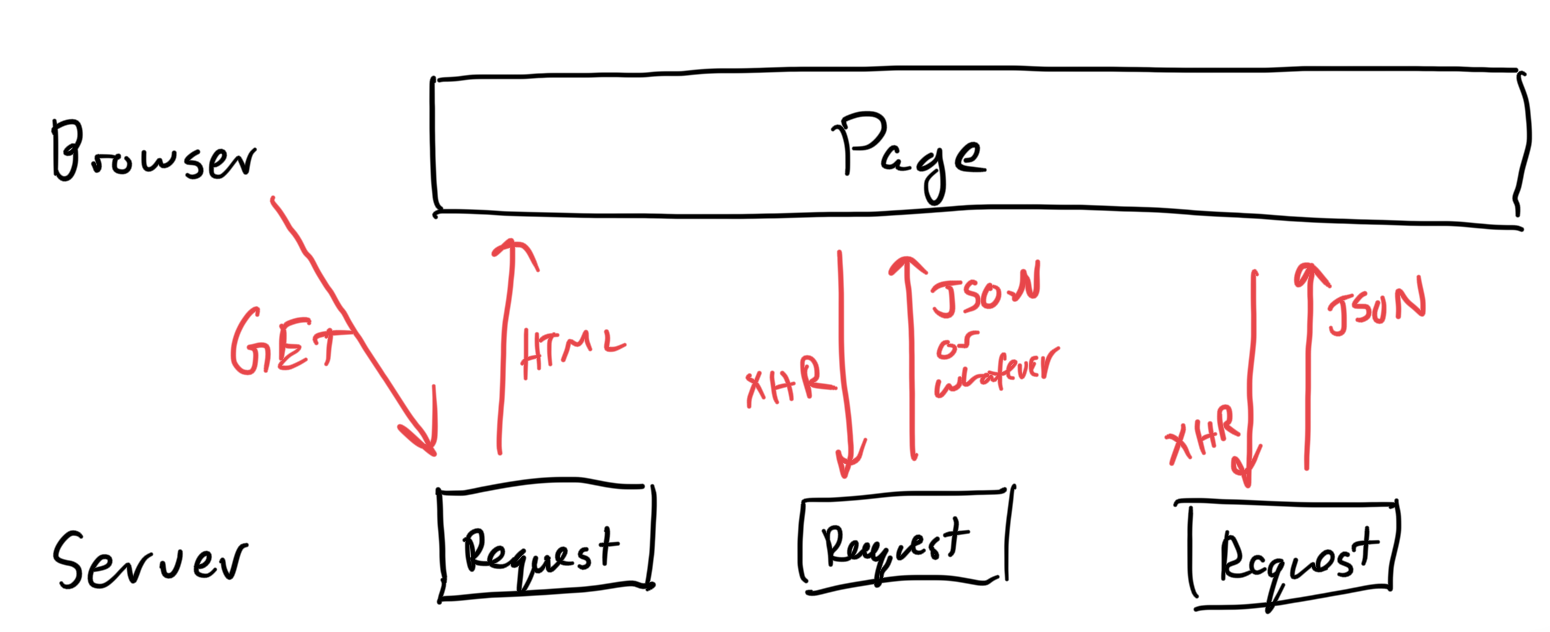
\includegraphics{im/security-spa.png}
\caption{The architecture of a single-page application leveraging
  \texttt{XMLHttpRequest}.}\label{fig:XMLHttpRequest}
\end{figure}

\begin{bookblock}{further}
\texttt{XMLHttpRequest} objects have
\href{https://developer.mozilla.org/en-US/docs/Web/API/XMLHttpRequest/setRequestHeader}{\texttt{setRequestHeader}}
and
\href{https://developer.mozilla.org/en-US/docs/Web/API/XMLHttpRequest/getResponseHeader}{\texttt{getResponseHeader}}
methods to control HTTP headers. However, this could allow a script to
interfere with the cookie mechanism or with other security measures, so
some
\href{https://developer.mozilla.org/en-US/docs/Glossary/Forbidden_header_name}{request}
and
\href{https://developer.mozilla.org/en-US/docs/Glossary/Forbidden_response_header_name}{response}
headers are not accessible from JavaScript.
\end{bookblock}

\hypertarget{same-origin-policy}{%
\section{Same-Origin Policy}\label{same-origin-policy}}

However, new capabilities lead to new responsibilities. HTTP requests
sent with \texttt{XMLHttpRequest} include cookies. This is by design:
when you ``like'' something, the server needs to associate the ``like''
to your account. But it also means that \texttt{XMLHttpRequest} can
access private data, and thus there is a need to protect it.

Let's imagine an attacker wants to know your username on our guest book
server. When you're logged in, the guest book includes your username on
the page (where it says ``Hello, so and so''), so reading the guest book
with your cookies is enough to determine your username.

With \texttt{XMLHttpRequest}, an attacker's website\footnote{Why is the
  user on the attacker's site? Perhaps it has funny memes, or it's been
  hacked and is being used for the attack against its will, or perhaps
  the evildoer paid for ads on sketchy websites where users have low
  standards for security anyway.} could request the guest book page:
\begin{bookblock*}{notcode}
\begin{Shaded}
\begin{Highlighting}[]
\NormalTok{x }\OperatorTok{=} \KeywordTok{new} \BuiltInTok{XMLHttpRequest}\NormalTok{()}\OperatorTok{;}
\NormalTok{x}\OperatorTok{.}\FunctionTok{open}\NormalTok{(}\StringTok{"GET"}\OperatorTok{,} \StringTok{"http://localhost:8000/"}\OperatorTok{,} \KeywordTok{false}\NormalTok{)}\OperatorTok{;}
\NormalTok{x}\OperatorTok{.}\FunctionTok{send}\NormalTok{()}\OperatorTok{;}
\NormalTok{user }\OperatorTok{=}\NormalTok{ x}\OperatorTok{.}\AttributeTok{responseText}\OperatorTok{.}\FunctionTok{split}\NormalTok{(}\StringTok{" "}\NormalTok{)[}\DecValTok{2}\NormalTok{]}\OperatorTok{.}\FunctionTok{split}\NormalTok{(}\StringTok{"\textless{}"}\NormalTok{)[}\DecValTok{0}\NormalTok{]}\OperatorTok{;}
\end{Highlighting}
\end{Shaded}
\end{bookblock*}
\noindent The issue here is that one server's web page content is being sent to a
script running on a website delivered by another server. Since the
content is derived from cookies, this leaks private data.

To prevent issues like this, browsers have a
\href{https://developer.mozilla.org/en-US/docs/Web/Security/Same-origin_policy}{\emph{same-origin
policy}}, which says that requests like
\texttt{XMLHttpRequest}\footnote{Some kinds of request are not subject
  to the same-origin policy (most prominently CSS and JavaScript files
  linked from a web page); conversely, the same-origin policy also
  governs JavaScript interactions with \texttt{iframe}s, images,
  \texttt{localStorage} and many other browser features.} can only go to
web pages on the same ``origin''---scheme, hostname, and
port.\footnote{You may have noticed that this is not the same definition
  of ``website'' as cookies use: cookies don't care about scheme or
  port! This seems to be an oversight or incongruity left over from the
  messy early web.} This way, % one
a website's private data has to stay on
that website, and cannot be leaked to an attacker on another server.

Let's implement the same-origin policy for our browser. We'll need to
compare the URL of the request to the URL of the page we are on:
\begin{Shaded}
\begin{Highlighting}[]
\KeywordTok{class}\NormalTok{ JSContext:}
    \KeywordTok{def}\NormalTok{ XMLHttpRequest\_send(}\VariableTok{self}\NormalTok{, method, url, body):}
        \CommentTok{\# ...}
        \ControlFlowTok{if}\NormalTok{ full\_url.origin() }\OperatorTok{!=} \VariableTok{self}\NormalTok{.tab.url.origin():}
            \ControlFlowTok{raise} \PreprocessorTok{Exception}\NormalTok{(}\StringTok{"Cross{-}origin XHR request not allowed"}\NormalTok{)}
        \CommentTok{\# ...}
\end{Highlighting}
\end{Shaded}
The \texttt{origin} function can just strip off the path from a URL:
\begin{Shaded}
\begin{Highlighting}[]
\KeywordTok{class}\NormalTok{ URL:}
    \KeywordTok{def}\NormalTok{ origin(}\VariableTok{self}\NormalTok{):}
        \ControlFlowTok{return} \VariableTok{self}\NormalTok{.scheme }\OperatorTok{+} \StringTok{"://"} \OperatorTok{+} \VariableTok{self}\NormalTok{.host }\OperatorTok{+} \StringTok{":"} \OperatorTok{+} \BuiltInTok{str}\NormalTok{(}\VariableTok{self}\NormalTok{.port)}
\end{Highlighting}
\end{Shaded}

Now an attacker can't read the guest book web page. But can they write
to it? Actually \ldots{}

\begin{bookblock}{further}
One interesting form of the same-origin policy involves images and the
HTML \texttt{\textless{}canvas\textgreater{}} element. The
\href{https://developer.mozilla.org/en-US/docs/Web/API/CanvasRenderingContext2D/drawImage}{\texttt{drawImage}
method} allows drawing an image to a canvas, even if that image was
loaded from another origin. But to prevent that image from being read
back with
\href{https://developer.mozilla.org/en-US/docs/Web/API/CanvasRenderingContext2D/getImageData}{\texttt{getImageData}}
or related methods, writing cross-origin data to a canvas
\href{https://developer.mozilla.org/en-US/docs/Web/HTML/CORS_enabled_image}{taints}
it, blocking read methods.
\end{bookblock}

\hypertarget{cross-site-request-forgery}{%
\section{Cross-Site Request Forgery}\label{cross-site-request-forgery}}

The same-origin policy prevents cross-origin \texttt{XMLHttpRequest}
calls. But the same-origin policy doesn't apply to normal browser
actions like clicking a link or filling out a form. This enables an
exploit called \emph{cross-site request forgery}, often shortened to
CSRF.

In cross-site request forgery, instead of using \texttt{XMLHttpRequest},
the attacker uses a form that submits to the guest book:
\begin{bookblock*}{notcode}
\begin{Shaded}
\begin{Highlighting}[]
\DataTypeTok{\textless{}}\KeywordTok{form}\OtherTok{ action}\OperatorTok{=}\StringTok{"http://localhost:8000/add"}\OtherTok{ method}\OperatorTok{=}\StringTok{post}\DataTypeTok{\textgreater{}}
  \DataTypeTok{\textless{}}\KeywordTok{p}\DataTypeTok{\textgreater{}\textless{}}\KeywordTok{input}\OtherTok{ name}\OperatorTok{=}\StringTok{guest}\DataTypeTok{\textgreater{}\textless{}/}\KeywordTok{p}\DataTypeTok{\textgreater{}}
  \DataTypeTok{\textless{}}\KeywordTok{p}\DataTypeTok{\textgreater{}\textless{}}\KeywordTok{button}\DataTypeTok{\textgreater{}}\NormalTok{Sign the book!}\DataTypeTok{\textless{}/}\KeywordTok{button}\DataTypeTok{\textgreater{}\textless{}/}\KeywordTok{p}\DataTypeTok{\textgreater{}}
\DataTypeTok{\textless{}/}\KeywordTok{form}\DataTypeTok{\textgreater{}}
\end{Highlighting}
\end{Shaded}
\end{bookblock*}
\noindent Even though this form is on the evildoer's website, when you submit the
form, the browser will make an HTTP request to the \emph{guest book}.
And that means it will send its guest book cookies, so it will be logged
in, so the guest book code will allow a post. But the user has no way of
knowing which server a form submits to---the attacker's web page could
have misrepresented that---so they may have posted something they didn't
mean to.\footnote{Even worse, the form submission could be triggered by
  JavaScript, with the user not involved at all. And this kind of attack
  can be further disguised by hiding the entry widget, pre-filling the
  post, and styling the button to look like a normal link.}

Of course, the attacker can't read the response, so this doesn't leak
private data to the attacker. But it can allow the attacker to
\emph{act} as the user! Posting a comment this way is not too scary
(though shady advertisers will pay for it!), but posting a bank
transaction is. And if the website has a change-of-password form, there
could even be a way to take control of the account.

Unfortunately, we can't just apply the same-origin policy to form
submissions.\footnote{For example, many search forms on websites submit
  to Google, because those websites don't have their own search engines.}
So how do we defend against this attack?
To start with, there are things the server can do. The usual advice is
to give a unique identity to every form the server serves, and make sure
that every POST request comes from one of them. The way to do that is to
embed a secret value, called a \emph{nonce}, into the form, and to
reject form submissions that don't come with the right secret
value.\footnote{Note the similarity to cookies, except that instead of
  granting identity to browsers, we grant one to forms. Like a cookie, a
  nonce can be stolen with cross-site scripting.} You can only get a
nonce from the server, and the nonce is tied to the user
session,\footnote{It's important that nonces are associated with the
  particular user. Otherwise, the attacker can generate a nonce for
  \emph{themselves} and insert it into a form meant for the \emph{user}.}
so the attacker could not embed it in their form.

To implement this fix, generate a nonce and save it in the user session
when a form is requested:\footnote{Usually
  \texttt{\textless{}input\ type=hidden\textgreater{}} is invisible,
  though our browser doesn't support this.}
\begin{Shaded}
\begin{Highlighting}[]
\KeywordTok{def}\NormalTok{ show\_comments(session):}
    \CommentTok{\# ...}
    \ControlFlowTok{if} \StringTok{"user"} \KeywordTok{in}\NormalTok{ session:}
\NormalTok{        nonce }\OperatorTok{=} \BuiltInTok{str}\NormalTok{(random.random())[}\DecValTok{2}\NormalTok{:]}
\NormalTok{        session[}\StringTok{"nonce"}\NormalTok{] }\OperatorTok{=}\NormalTok{ nonce}
        \CommentTok{\# ...}
\NormalTok{        out }\OperatorTok{+=} \StringTok{"\textless{}input name=nonce type=hidden value="} \OperatorTok{+}\NormalTok{ nonce }\OperatorTok{+} \StringTok{"\textgreater{}"}
\end{Highlighting}
\end{Shaded}
When a form is submitted, the server checks that the right nonce is
submitted with it:\footnote{In real websites it's usually best to allow
  one user to have multiple active nonces, so that a user can open two
  forms in two tabs without that overwriting the valid nonce. To prevent
  the nonce set from growing over time, you'd have nonces expire after a
  while. I'm skipping this here, because it's not the focus of this
  chapter.}
\begin{Shaded}
\begin{Highlighting}[]
\KeywordTok{def}\NormalTok{ add\_entry(session, params):}
    \ControlFlowTok{if} \StringTok{"nonce"} \KeywordTok{not} \KeywordTok{in}\NormalTok{ session }\KeywordTok{or} \StringTok{"nonce"} \KeywordTok{not} \KeywordTok{in}\NormalTok{ params: }\ControlFlowTok{return}
    \ControlFlowTok{if}\NormalTok{ session[}\StringTok{"nonce"}\NormalTok{] }\OperatorTok{!=}\NormalTok{ params[}\StringTok{"nonce"}\NormalTok{]: }\ControlFlowTok{return}
    \CommentTok{\# ...}
\end{Highlighting}
\end{Shaded}

Now this form can't be submitted except from our website. Repeat this
nonce fix for each form in the application, and it'll be secure from
CSRF attacks. But server-side solutions are fragile (what if you forget
a form?) and relying on every website out there to do it right is a pipe
dream. It'd be better for the browser to provide a fail-safe backup.

\begin{bookblock}{further}
One unusual attack, similar in spirit to cross-site request forgery, is
\href{https://owasp.org/www-community/attacks/Clickjacking}{click-jacking}.
In this attack, an external site in a transparent \texttt{iframe} is
positioned over the attacker's site. The user thinks they are clicking
around one site, but they actually take actions on a different one.
Nowadays, sites can prevent this with the
\href{https://developer.mozilla.org/en-US/docs/Web/HTTP/Headers/Content-Security-Policy/frame-ancestors}{\texttt{frame-ancestors}
directive} to \texttt{Content-Security-Policy} or the older
\href{https://developer.mozilla.org/en-US/docs/Web/HTTP/Headers/X-Frame-Options}{\texttt{X-Frame-Options}
header}.
\end{bookblock}

\hypertarget{samesite-cookies}{%
\section{SameSite Cookies}\label{samesite-cookies}}

For form submissions, that fail-safe solution is \texttt{SameSite}
cookies. The idea is that if a server marks its cookies
\texttt{SameSite}, the browser will not send them in cross-site form
submissions.\footnote{At the time of % this
  writing the \texttt{SameSite}
  cookie standard is still in a draft stage, and not all browsers
  implement that draft fully. So it's possible % for
  that this section may % to
  become out of date, though some kind of \texttt{SameSite} cookies will
  probably be ratified. The
  \href{https://developer.mozilla.org/en-US/docs/Web/HTTP/Headers/Set-Cookie/SameSite}{MDN
  page} is helpful for checking the current status of \texttt{SameSite}
  cookies.}

A cookie is marked \texttt{SameSite} in the \texttt{Set-Cookie} header
like this:
\begin{bookblock*}{notcode}
\begin{verbatim}
Set-Cookie: foo=bar; SameSite=Lax
\end{verbatim}
\end{bookblock*}
\noindent The \texttt{SameSite} attribute can take the value \texttt{Lax},
\texttt{Strict}, or \texttt{None}, and as I write, browsers have and
plan different defaults. Our browser will implement only \texttt{Lax}
and \texttt{None}, and default to \texttt{None}. When \texttt{SameSite}
is set to \texttt{Lax}, the cookie is not sent on cross-site
\texttt{POST} requests, but is sent on same-site \texttt{POST} or
cross-site \texttt{GET} requests.\footnote{Cross-site \texttt{GET}
  requests are also known as ``clicking a link'', which is why those are
  allowed in \texttt{Lax} mode. The \texttt{Strict} version of
  \texttt{SameSite} blocks these too, but you need to design your web
  application carefully for this to work.}

First, let's modify \texttt{COOKIE\_JAR} to store cookie/parameter
pairs, and then parse those parameters out of \texttt{Set-Cookie}
headers:
\begin{Shaded}
\begin{Highlighting}[]
\KeywordTok{def}\NormalTok{ request(}\VariableTok{self}\NormalTok{, payload}\OperatorTok{=}\VariableTok{None}\NormalTok{):}
    \ControlFlowTok{if} \StringTok{"set{-}cookie"} \KeywordTok{in}\NormalTok{ response\_headers:}
\NormalTok{        cookie }\OperatorTok{=}\NormalTok{ response\_headers[}\StringTok{"set{-}cookie"}\NormalTok{]}
\NormalTok{        params }\OperatorTok{=}\NormalTok{ \{\}}
        \ControlFlowTok{if} \StringTok{";"} \KeywordTok{in}\NormalTok{ cookie:}
\NormalTok{            cookie, rest }\OperatorTok{=}\NormalTok{ cookie.split(}\StringTok{";"}\NormalTok{, }\DecValTok{1}\NormalTok{)}
            \ControlFlowTok{for}\NormalTok{ param }\KeywordTok{in}\NormalTok{ rest.split(}\StringTok{";"}\NormalTok{):}
                \ControlFlowTok{if} \StringTok{\textquotesingle{}=\textquotesingle{}} \KeywordTok{in}\NormalTok{ param:}
\NormalTok{                    param, value }\OperatorTok{=}\NormalTok{ param.split(}\StringTok{"="}\NormalTok{, }\DecValTok{1}\NormalTok{)}
                \ControlFlowTok{else}\NormalTok{:}
\NormalTok{                    value }\OperatorTok{=} \StringTok{"true"}
\NormalTok{                params[param.strip().casefold()] }\OperatorTok{=}\NormalTok{ value.casefold()}
\NormalTok{        COOKIE\_JAR[}\VariableTok{self}\NormalTok{.host] }\OperatorTok{=}\NormalTok{ (cookie, params)}
\end{Highlighting}
\end{Shaded}
When sending a cookie in an HTTP request, the browser only sends the
cookie value, not the parameters:
\begin{Shaded}
\begin{Highlighting}[]
\KeywordTok{def}\NormalTok{ request(}\VariableTok{self}\NormalTok{, payload}\OperatorTok{=}\VariableTok{None}\NormalTok{):}
    \ControlFlowTok{if} \VariableTok{self}\NormalTok{.host }\KeywordTok{in}\NormalTok{ COOKIE\_JAR:}
\NormalTok{        cookie, params }\OperatorTok{=}\NormalTok{ COOKIE\_JAR[}\VariableTok{self}\NormalTok{.host]}
\NormalTok{        request }\OperatorTok{+=} \StringTok{"Cookie: }\SpecialCharTok{\{\}}\CharTok{\textbackslash{}r\textbackslash{}n}\StringTok{"}\NormalTok{.}\BuiltInTok{format}\NormalTok{(cookie)}
\end{Highlighting}
\end{Shaded}

This stores the \texttt{SameSite} parameter of a cookie. But to actually
use it, we need to know which site an HTTP request is being made from.
Let's add a new \texttt{referrer} parameter to \texttt{request}
to track that:\footnote{The ``referrer'' is the web page that ``referred'' our
  browser to make the current request. \texttt{SameSite} cookies are
  actually supposed to
  \href{https://datatracker.ietf.org/doc/html/draft-ietf-httpbis-cookie-same-site-00\#section-2.1}{use
  the ``top-level site''}, not the referrer, to determine if the cookies
  should be sent, but the differences are subtle and I'm skipping them
  for simplicity.}
\begin{Shaded}
\begin{Highlighting}[]
\KeywordTok{class}\NormalTok{ URL:}
    \KeywordTok{def}\NormalTok{ request(}\VariableTok{self}\NormalTok{, referrer, payload}\OperatorTok{=}\VariableTok{None}\NormalTok{):}
        \CommentTok{\# ...}
\end{Highlighting}
\end{Shaded}
Our browser calls \texttt{request} in three places, and we need to send
the top-level URL in each case. At the top of \texttt{load}, it makes
the initial request to a page. Modify it like so:
\begin{Shaded}
\begin{Highlighting}[]
\KeywordTok{class}\NormalTok{ Tab:}
    \KeywordTok{def}\NormalTok{ load(}\VariableTok{self}\NormalTok{, url, payload}\OperatorTok{=}\VariableTok{None}\NormalTok{):}
\NormalTok{        headers, body }\OperatorTok{=}\NormalTok{ url.request(}\VariableTok{self}\NormalTok{.url, payload)}
        \CommentTok{\# ...}
\end{Highlighting}
\end{Shaded}
Here, \texttt{url} is the new URL to visit, but \texttt{self.url} is the
URL of the page % where
the request comes from. Make sure this line comes
at the top of \texttt{load}, before \texttt{self.url} is changed!

Later, the browser loads styles and scripts with more \texttt{request}
calls:
\begin{Shaded}
\begin{Highlighting}[]
\KeywordTok{class}\NormalTok{ Tab:}
    \KeywordTok{def}\NormalTok{ load(}\VariableTok{self}\NormalTok{, url, payload}\OperatorTok{=}\VariableTok{None}\NormalTok{):}
        \CommentTok{\# ...}
        \ControlFlowTok{for}\NormalTok{ script }\KeywordTok{in}\NormalTok{ scripts:}
            \CommentTok{\# ...}
            \ControlFlowTok{try}\NormalTok{:}
\NormalTok{                header, body }\OperatorTok{=}\NormalTok{ script\_url.request(url)}
            \ControlFlowTok{except}\NormalTok{:}
                \ControlFlowTok{continue}
            \CommentTok{\# ...}
        \CommentTok{\# ...}
        \ControlFlowTok{for}\NormalTok{ link }\KeywordTok{in}\NormalTok{ links:}
            \CommentTok{\# ...}
            \ControlFlowTok{try}\NormalTok{:}
\NormalTok{                header, body }\OperatorTok{=}\NormalTok{ style\_url.request(url)}
            \ControlFlowTok{except}\NormalTok{:}
                \ControlFlowTok{continue}
            \CommentTok{\# ...}
        \CommentTok{\# ...}
\end{Highlighting}
\end{Shaded}
For these requests the top-level URL is the new URL being loaded. That's
because it is the new page that made us request these particular styles
and scripts, so it defines which of those resources are on the same
site.

Similarly, \texttt{XMLHttpRequest}-triggered requests use the tab URL as
their top-level URL:
\begin{Shaded}
\begin{Highlighting}[]
\KeywordTok{class}\NormalTok{ JSContext:}
    \KeywordTok{def}\NormalTok{ XMLHttpRequest\_send(}\VariableTok{self}\NormalTok{, method, url, body):}
        \CommentTok{\# ...}
\NormalTok{        headers, out }\OperatorTok{=}\NormalTok{ full\_url.request(}\VariableTok{self}\NormalTok{.tab.url, body)}
        \CommentTok{\# ...}
\end{Highlighting}
\end{Shaded}

The \texttt{request} function can now check the \texttt{referrer}
argument before sending \texttt{SameSite} cookies. Remember that
\texttt{SameSite} cookies are only sent for \texttt{GET} requests or if
the new URL and the top-level URL have the same host name:\footnote{As I
  write this, some browsers also check that the new URL and the
  top-level URL have the same scheme and some browsers ignore
  subdomains, so that \texttt{www.foo.com} and \texttt{login.foo.com}
  are considered the ``same site''. If cookies were invented today,
  they'd probably be specific to URL origins (in fact, there is
  \href{https://github.com/sbingler/Origin-Bound-Cookies}{an effort to
  do just that}), much like % CSP
  content security policies, but alas historical
  contingencies and backward compatibility force rules that are more
  complex but easier to deploy.}
\begin{Shaded}
\begin{Highlighting}[]
\KeywordTok{def}\NormalTok{ request(}\VariableTok{self}\NormalTok{, referrer, payload}\OperatorTok{=}\VariableTok{None}\NormalTok{):}
    \ControlFlowTok{if} \VariableTok{self}\NormalTok{.host }\KeywordTok{in}\NormalTok{ COOKIE\_JAR:}
        \CommentTok{\# ...}
\NormalTok{        cookie, params }\OperatorTok{=}\NormalTok{ COOKIE\_JAR[}\VariableTok{self}\NormalTok{.host]}
\NormalTok{        allow\_cookie }\OperatorTok{=} \VariableTok{True}
        \ControlFlowTok{if}\NormalTok{ referrer }\KeywordTok{and}\NormalTok{ params.get(}\StringTok{"samesite"}\NormalTok{, }\StringTok{"none"}\NormalTok{) }\OperatorTok{==} \StringTok{"lax"}\NormalTok{:}
            \ControlFlowTok{if}\NormalTok{ method }\OperatorTok{!=} \StringTok{"GET"}\NormalTok{:}
\NormalTok{                allow\_cookie }\OperatorTok{=} \VariableTok{self}\NormalTok{.host }\OperatorTok{==}\NormalTok{ referrer.host}
        \ControlFlowTok{if}\NormalTok{ allow\_cookie:}
\NormalTok{            request }\OperatorTok{+=} \StringTok{"Cookie: }\SpecialCharTok{\{\}}\CharTok{\textbackslash{}r\textbackslash{}n}\StringTok{"}\NormalTok{.}\BuiltInTok{format}\NormalTok{(cookie)}
        \CommentTok{\# ...}
\end{Highlighting}
\end{Shaded}
Note that we check whether the \texttt{referrer} is set---it
won't be when we're loading the first web page in a new tab.

Our guest book can now mark its cookies \texttt{SameSite}:
\begin{Shaded}
\begin{Highlighting}[]
\KeywordTok{def}\NormalTok{ handle\_connection(conx):}
    \ControlFlowTok{if} \StringTok{\textquotesingle{}cookie\textquotesingle{}} \KeywordTok{not} \KeywordTok{in}\NormalTok{ headers:}
\NormalTok{        template }\OperatorTok{=} \StringTok{"Set{-}Cookie: token=}\SpecialCharTok{\{\}}\StringTok{; SameSite=Lax}\CharTok{\textbackslash{}r\textbackslash{}n}\StringTok{"}
\NormalTok{        response }\OperatorTok{+=}\NormalTok{ template.}\BuiltInTok{format}\NormalTok{(token)}
\end{Highlighting}
\end{Shaded}

\texttt{SameSite} provides a kind of ``defense in depth'', a fail-safe
that makes sure that even if we forgot a nonce somewhere, we're still
secure against CSRF attacks. But don't remove the nonces we added
earlier! They're important for older browsers and are more flexible in
cases like multiple domains.

\begin{bookblock}{further}
The web was not initially designed around security, which has led to
some \href{https://jakearchibald.com/2021/cors/}{awkward patches} after
the fact. These patches may be ugly, but a dedication to backward
compatibility is a strength of the web, and at least newer APIs can be
designed around more consistent policies.

To this end, while there is a full specification for \texttt{SameSite},
it is still the case that real browsers support different subsets of the
feature or different defaults. For example, Chrome defaults to
\texttt{Lax}, but Firefox and Safari do not. Likewise, Chrome uses the
scheme (\texttt{https} or \texttt{http}) as part of the definition of a
``site'',\footnotemark\ but other
browsers may not. The main reason for this situation is the need to
maintain backward compatibility with existing websites.
\end{bookblock}
\footnotetext{This is called ``schemeful same-site''.}

\hypertarget{cross-site-scripting}{%
\section{Cross-Site Scripting}\label{cross-site-scripting}}

Now other websites can't misuse our browser's cookies to read or write
private data. This seems secure! But what about \emph{our own} website?
With cookies accessible from JavaScript, any scripts run on our browser
could, in principle, read the cookie value. This might seem
benign---doesn't our browser only run \texttt{comment.js}? But in
fact \ldots{}

A web service needs to defend itself from being \emph{misused}. Consider
the code in our guest book that outputs guest book entries:
\begin{Shaded}
\begin{Highlighting}[]
\NormalTok{out }\OperatorTok{+=} \StringTok{"\textless{}p\textgreater{}"} \OperatorTok{+}\NormalTok{ entry }\OperatorTok{+} \StringTok{"}\CharTok{\textbackslash{}n}\StringTok{"}
\NormalTok{out }\OperatorTok{+=} \StringTok{"\textless{}i\textgreater{}by "} \OperatorTok{+}\NormalTok{ who }\OperatorTok{+} \StringTok{"\textless{}/i\textgreater{}\textless{}/p\textgreater{}"}
\end{Highlighting}
\end{Shaded}
Note that \texttt{entry} can be anything, including anything the user
might stick into our comment form. That includes HTML tags, like a
custom \texttt{\textless{}script\textgreater{}} tag! So, a malicious
user could post this comment:
\begin{Shaded}
\begin{Highlighting}[]
\NormalTok{Hi! }\DataTypeTok{\textless{}}\KeywordTok{script}\OtherTok{ src}\OperatorTok{=}\StringTok{"http://my{-}server/evil.js"}\DataTypeTok{\textgreater{}\textless{}/}\KeywordTok{script}\DataTypeTok{\textgreater{}}
\end{Highlighting}
\end{Shaded}
\noindent The server would then output this HTML:
\begin{Shaded}
\begin{Highlighting}[]
\DataTypeTok{\textless{}}\KeywordTok{p}\DataTypeTok{\textgreater{}}\NormalTok{Hi! }\DataTypeTok{\textless{}}\KeywordTok{script}\OtherTok{ src}\OperatorTok{=}\StringTok{"http://my{-}server/evil.js"}\DataTypeTok{\textgreater{}\textless{}/}\KeywordTok{script}\DataTypeTok{\textgreater{}}
\DataTypeTok{\textless{}}\KeywordTok{i}\DataTypeTok{\textgreater{}}\NormalTok{by crashoverride}\DataTypeTok{\textless{}/}\KeywordTok{i}\DataTypeTok{\textgreater{}\textless{}/}\KeywordTok{p}\DataTypeTok{\textgreater{}}
\end{Highlighting}
\end{Shaded}
\noindent Every user's browser would then download and run the \texttt{evil.js}
script, which can send\footnote{A site's cookies and cookie parameters
  are available to scripts running on that site through the
  \href{https://developer.mozilla.org/en-US/docs/Web/API/Document/cookie}{\texttt{document.cookie}}
  API. % }\footnote{
  See % the exercise on \texttt{Access-Control-Allow-Origin}
  Exercise~\ref{ex:CORS} for more details on how web
  servers can \emph{opt in} to allowing cross-origin requests. To steal
  cookies, it's the attacker's server that would to opt in to receiving
  stolen cookies. Or, in a real browser, \texttt{evil.js} could add
  images or scripts to the page to trigger additional requests. % }\footnote{
  In
  our limited browser the attack has to be a little clunkier, but the
  evil script can still, for example, replace the whole page with a link
  that goes to their site and includes the token value in the URL.
  You've seen ``please click to continue'' screens and have clicked
  through unthinkingly; your users will too.} the cookies to the
attacker. The attacker could then impersonate other users, posting as
them or misusing any other capabilities those users had.

The core problem here is that user comments are supposed to be data, but
the browser is interpreting them as code. In web applications, this kind
of exploit is usually called \emph{cross-site scripting} (often written
``XSS''), though misinterpreting data as code is a common security issue
in all kinds of programs.

The standard fix is to encode the data so that it can't be interpreted
as code. For example, in HTML, you can write \texttt{\&lt;} to display a
less-than sign.\footnote{You may have implemented this in % a \href{http.md\#exercises}{Chapter 1 exercise}
  Exercise~\ref{ex:Entities}.} Python has an \texttt{html} module for this kind of encoding:
\begin{Shaded}
\begin{Highlighting}[]
\ImportTok{import}\NormalTok{ html}

\KeywordTok{def}\NormalTok{ show\_comments(session):}
    \CommentTok{\# ...}
\NormalTok{    out }\OperatorTok{+=} \StringTok{"\textless{}p\textgreater{}"} \OperatorTok{+}\NormalTok{ html.escape(entry) }\OperatorTok{+} \StringTok{"}\CharTok{\textbackslash{}n}\StringTok{"}
\NormalTok{    out }\OperatorTok{+=} \StringTok{"\textless{}i\textgreater{}by "} \OperatorTok{+}\NormalTok{ html.escape(who) }\OperatorTok{+} \StringTok{"\textless{}/i\textgreater{}\textless{}/p\textgreater{}"}
    \CommentTok{\# ...}
\end{Highlighting}
\end{Shaded}
This is a good fix, and every application should be careful to do this
escaping. But if you forget to encode any text anywhere---that's a
security bug. So browsers provide additional layers of defense.

\begin{bookblock}{further}
Since the
{CSS parser} we implemented in Chapter~\ref{ch:ApplyingAuthorStyles} is very permissive, some HTML
pages also parse as valid CSS. This leads to an attack: include an
external HTML page as a style sheet and observe the styling it applies.
A
\href{https://owasp.org/www-pdf-archive/OWASPLondon20161124_JSON_Hijacking_Gareth_Heyes.pdf}{similar
attack} involves including external JSON files as scripts. Setting a
\texttt{Content-Type} header can prevent this sort of attack thanks to
browsers'
\href{https://chromium.googlesource.com/chromium/src/+/refs/heads/main/services/network/cross_origin_read_blocking_explainer.md}{Cross-Origin
Read Blocking} policy.
\end{bookblock}

\hypertarget{content-security-policy}{%
\section{Content Security Policy}\label{content-security-policy}}

One such layer is the \texttt{Content-Security-Policy} header. The full
specification for this header is quite complex, but in the simplest
case, the header is set to the keyword \texttt{default-src} followed by
a space-separated list of servers:
\begin{bookblock*}{notcode}
\begin{verbatim}
Content-Security-Policy: default-src http://example.org
\end{verbatim}
\end{bookblock*}
\noindent This header asks the browser not to load any resources (including CSS,
JavaScript, images, and so on) except from the listed origins. If our
guest book used \texttt{Content-Security-Policy}, even if an attacker
managed to get a \texttt{\textless{}script\textgreater{}} added to the
page, the browser would refuse to load and run that script.

Let's implement support for this header. First, we'll need
\texttt{request} to return the response headers:
\begin{Shaded}
\begin{Highlighting}[]
\KeywordTok{class}\NormalTok{ URL:}
    \KeywordTok{def}\NormalTok{ request(}\VariableTok{self}\NormalTok{, referrer, payload}\OperatorTok{=}\VariableTok{None}\NormalTok{):}
        \CommentTok{\# ...}
        \ControlFlowTok{return}\NormalTok{ response\_headers, content}
\end{Highlighting}
\end{Shaded}
Make sure to update all existing uses of \texttt{request} to ignore the
headers.

Next, we'll need to extract and parse the
\texttt{Content-Security-Policy} header when loading a page:\footnote{In
  real browsers \texttt{Content-Security-Policy} can also list
  scheme-generic URLs and other sources like
  \texttt{\textquotesingle{}self\textquotesingle{}}. And there are
  keywords other than \texttt{default-src}, to restrict styles, scripts,
  and \texttt{XMLHttpRequest}s each to their own set of URLs.}
\begin{Shaded}
\begin{Highlighting}[]
\KeywordTok{class}\NormalTok{ Tab:}
    \KeywordTok{def}\NormalTok{ load(}\VariableTok{self}\NormalTok{, url, payload}\OperatorTok{=}\VariableTok{None}\NormalTok{):}
        \CommentTok{\# ...}
        \VariableTok{self}\NormalTok{.allowed\_origins }\OperatorTok{=} \VariableTok{None}
        \ControlFlowTok{if} \StringTok{"content{-}security{-}policy"} \KeywordTok{in}\NormalTok{ headers:}
\NormalTok{            csp }\OperatorTok{=}\NormalTok{ headers[}\StringTok{"content{-}security{-}policy"}\NormalTok{].split()}
            \ControlFlowTok{if} \BuiltInTok{len}\NormalTok{(csp) }\OperatorTok{\textgreater{}} \DecValTok{0} \KeywordTok{and}\NormalTok{ csp[}\DecValTok{0}\NormalTok{] }\OperatorTok{==} \StringTok{"default{-}src"}\NormalTok{:}
                \VariableTok{self}\NormalTok{.allowed\_origins }\OperatorTok{=}\NormalTok{ []}
                \ControlFlowTok{for}\NormalTok{ origin }\KeywordTok{in}\NormalTok{ csp[}\DecValTok{1}\NormalTok{:]:}
                    \VariableTok{self}\NormalTok{.allowed\_origins.append(URL(origin).origin())}
        \CommentTok{\# ...}
\end{Highlighting}
\end{Shaded}
This parsing needs to happen \emph{before} we request any JavaScript or
CSS, because we now need to check whether those requests are allowed:
\begin{Shaded}
\begin{Highlighting}[]
\KeywordTok{class}\NormalTok{ Tab:}
    \KeywordTok{def}\NormalTok{ load(}\VariableTok{self}\NormalTok{, url, payload}\OperatorTok{=}\VariableTok{None}\NormalTok{):}
        \CommentTok{\# ...}
        \ControlFlowTok{for}\NormalTok{ script }\KeywordTok{in}\NormalTok{ scripts:}
\NormalTok{            script\_url }\OperatorTok{=}\NormalTok{ url.resolve(script)}
            \ControlFlowTok{if} \KeywordTok{not} \VariableTok{self}\NormalTok{.allowed\_request(script\_url):}
                \BuiltInTok{print}\NormalTok{(}\StringTok{"Blocked script"}\NormalTok{, script, }\StringTok{"due to CSP"}\NormalTok{)}
                \ControlFlowTok{continue}
            \CommentTok{\# ...}
\end{Highlighting}
\end{Shaded}
Note that we need to first resolve relative URLs to know if they're
allowed. Add a similar test to the CSS-loading code.

\texttt{XMLHttpRequest} URLs also need to be checked:\footnote{Note that
  when loading styles and scripts, our browser merely ignores blocked
  resources, while for blocked \texttt{XMLHttpRequest}s it throws an
  exception. That's because exceptions in \texttt{XMLHttpRequest} calls
  can be caught and handled in JavaScript.}
\begin{Shaded}
\begin{Highlighting}[]
\KeywordTok{class}\NormalTok{ JSContext:}
    \KeywordTok{def}\NormalTok{ XMLHttpRequest\_send(}\VariableTok{self}\NormalTok{, method, url, body):}
\NormalTok{        full\_url }\OperatorTok{=} \VariableTok{self}\NormalTok{.tab.url.resolve(url)}
        \ControlFlowTok{if} \KeywordTok{not} \VariableTok{self}\NormalTok{.tab.allowed\_request(full\_url):}
            \ControlFlowTok{raise} \PreprocessorTok{Exception}\NormalTok{(}\StringTok{"Cross{-}origin XHR blocked by CSP"}\NormalTok{)}
        \CommentTok{\# ...}
\end{Highlighting}
\end{Shaded}
The \texttt{allowed\_request} check needs to handle both the case of no
\texttt{Content-Security-Policy} and the case where there is one:
\begin{Shaded}
\begin{Highlighting}[]
\KeywordTok{class}\NormalTok{ Tab:}
    \KeywordTok{def}\NormalTok{ allowed\_request(}\VariableTok{self}\NormalTok{, url):}
        \ControlFlowTok{return} \VariableTok{self}\NormalTok{.allowed\_origins }\OperatorTok{==} \VariableTok{None} \KeywordTok{or} \OperatorTok{\textbackslash{}}
\NormalTok{            url.origin() }\KeywordTok{in} \VariableTok{self}\NormalTok{.allowed\_origins}
\end{Highlighting}
\end{Shaded}

The guest book can now send a \texttt{Content-Security-Policy} header:
\begin{Shaded}
\begin{Highlighting}[]
\KeywordTok{def}\NormalTok{ handle\_connection(conx):}
    \CommentTok{\# ...}
\NormalTok{    csp }\OperatorTok{=} \StringTok{"default{-}src http://localhost:8000"}
\NormalTok{    response }\OperatorTok{+=} \StringTok{"Content{-}Security{-}Policy: }\SpecialCharTok{\{\}}\CharTok{\textbackslash{}r\textbackslash{}n}\StringTok{"}\NormalTok{.}\BuiltInTok{format}\NormalTok{(csp)}
    \CommentTok{\# ...}
\end{Highlighting}
\end{Shaded}
To check that our implementation works, let's have the guest book
request a script from outside the list of allowed servers:
\begin{Shaded}
\begin{Highlighting}[]
\KeywordTok{def}\NormalTok{ show\_comments(session):}
    \CommentTok{\# ...}
\NormalTok{    out }\OperatorTok{+=} \StringTok{"\textless{}script src=https://example.com/evil.js\textgreater{}\textless{}/script\textgreater{}"}
    \CommentTok{\# ...}
\end{Highlighting}
\end{Shaded}
If you've got everything implemented correctly, the browser should block
the evil script\footnote{Needless to say, \texttt{example.com} does not
  actually host an \texttt{evil.js} file, and any request to it returns
  ``404 Not Found''.} and report so in the console.

So, are we done? Is the guest book totally secure? Uh\ \ldots\ no. There's
more---much, \emph{much} more---to web application security than what's
in this book. And just like the rest of this book, there are many other
browser mechanisms that touch on security and privacy. Let's settle for
this fact: the guest book is more secure than before.

\begin{bookblock}{further}
On a complicated site, deploying \texttt{Content-Security-Policy} can
accidentally break something. For this reason, browsers can
automatically report \texttt{Content-Security-Policy} violations to the
server, using the
\href{https://developer.mozilla.org/en-US/docs/Web/HTTP/Headers/Content-Security-Policy/report-to}{\texttt{report-to}
directive}. The
\href{https://developer.mozilla.org/en-US/docs/Web/HTTP/Headers/Content-Security-Policy-Report-Only}{\texttt{Content-Security-Policy-Report-Only}}
header asks the browser to report violations of the content security
policy \emph{without} actually blocking the requests.
\end{bookblock}

\hypertarget{summary}{%
\section{Summary}\label{KeepingDataPrivate-summary}}

We've added user data, in the form of cookies, to our browser, and
immediately had to bear the heavy burden of securing that data and
ensuring it was not misused. That involved:
\begin{itemize}
%\tightlist
\item
  mitigating cross-site \texttt{XMLHttpRequest}s with the same-origin
  policy;
\item
  mitigating cross-site request forgery with nonces and with
  \texttt{SameSite} cookies;
\item
  mitigating cross-site scripting with escaping and with
  \texttt{Content-Security-Policy}.
\end{itemize}
We've also seen the more general lesson that every increase in the
capabilities of a web browser also leads to an increase in its
responsibility to safeguard user data. Security is an ever-present
consideration throughout the design of a web browser.

\begin{bookblock}{warning}
The purpose of this book is to teach the \emph{internals of web
browsers}, not to teach web application security. There's much more
you'd want to do to make this guest book truly secure, let alone what
we'd need to do to avoid denial of service attacks or to handle spam and
malicious use. Please consult other sources before working on
security-critical code.
\end{bookblock}

\hypertarget{outline}{%
\section{Outline}\label{KeepingDataPrivate-outline}}

The complete set of functions, classes, and methods in our browser
should now look something like this:
\begin{Shaded}
\begin{Highlighting}[]
\NormalTok{WIDTH}
\NormalTok{HEIGHT}
\NormalTok{HSTEP}
\NormalTok{VSTEP}
\NormalTok{SCROLL\_STEP}
\NormalTok{FONTS}
\KeywordTok{def}\NormalTok{ get\_font(size, weight, slant)}
\KeywordTok{def}\NormalTok{ print\_tree(node, indent)}
\KeywordTok{class}\NormalTok{ HTMLParser:}
    \KeywordTok{def} \FunctionTok{\_\_init\_\_}\NormalTok{(body)}
    \KeywordTok{def}\NormalTok{ parse()}
    \KeywordTok{def}\NormalTok{ get\_attributes(text)}
    \KeywordTok{def}\NormalTok{ add\_text(text)}
\NormalTok{    SELF\_CLOSING\_TAGS}
    \KeywordTok{def}\NormalTok{ add\_tag(tag)}
\NormalTok{    HEAD\_TAGS}
    \KeywordTok{def}\NormalTok{ implicit\_tags(tag)}
    \KeywordTok{def}\NormalTok{ finish()}
\NormalTok{BLOCK\_ELEMENTS}
\KeywordTok{class}\NormalTok{ CSSParser:}
    \KeywordTok{def} \FunctionTok{\_\_init\_\_}\NormalTok{(s)}
    \KeywordTok{def}\NormalTok{ whitespace()}
    \KeywordTok{def}\NormalTok{ literal(literal)}
    \KeywordTok{def}\NormalTok{ word()}
    \KeywordTok{def}\NormalTok{ pair()}
    \KeywordTok{def}\NormalTok{ ignore\_until(chars)}
    \KeywordTok{def}\NormalTok{ body()}
    \KeywordTok{def}\NormalTok{ selector()}
    \KeywordTok{def}\NormalTok{ parse()}
\KeywordTok{class}\NormalTok{ TagSelector:}
    \KeywordTok{def} \FunctionTok{\_\_init\_\_}\NormalTok{(tag)}
    \KeywordTok{def}\NormalTok{ matches(node)}
\KeywordTok{class}\NormalTok{ DescendantSelector:}
    \KeywordTok{def} \FunctionTok{\_\_init\_\_}\NormalTok{(ancestor, descendant)}
    \KeywordTok{def}\NormalTok{ matches(node)}
\NormalTok{INHERITED\_PROPERTIES}
\KeywordTok{def}\NormalTok{ style(node, rules)}
\KeywordTok{def}\NormalTok{ cascade\_priority(rule)}
\KeywordTok{class}\NormalTok{ DrawText:}
    \KeywordTok{def} \FunctionTok{\_\_init\_\_}\NormalTok{(x1, y1, text, font, color)}
    \KeywordTok{def}\NormalTok{ execute(scroll, canvas)}
\KeywordTok{def}\NormalTok{ tree\_to\_list(tree, }\NormalTok{list}\NormalTok{)}
\KeywordTok{class}\NormalTok{ DrawLine:}
    \KeywordTok{def} \FunctionTok{\_\_init\_\_}\NormalTok{(x1, y1, x2, y2, color, thickness)}
    \KeywordTok{def}\NormalTok{ execute(scroll, canvas)}
\KeywordTok{class}\NormalTok{ DrawOutline:}
    \KeywordTok{def} \FunctionTok{\_\_init\_\_}\NormalTok{(rect, color, thickness)}
    \KeywordTok{def}\NormalTok{ execute(scroll, canvas)}
\KeywordTok{class}\NormalTok{ DrawRect:}
    \KeywordTok{def} \FunctionTok{\_\_init\_\_}\NormalTok{(rect, color)}
    \KeywordTok{def}\NormalTok{ execute(scroll, canvas)}
\KeywordTok{class}\NormalTok{ URL:}
    \KeywordTok{def} \FunctionTok{\_\_init\_\_}\NormalTok{(url)}
    \KeywordTok{def}\NormalTok{ request(referrer, payload)}
    \KeywordTok{def}\NormalTok{ resolve(url)}
    \KeywordTok{def}\NormalTok{ origin()}
\KeywordTok{class}\NormalTok{ Browser:}
    \KeywordTok{def} \FunctionTok{\_\_init\_\_}\NormalTok{()}
    \KeywordTok{def}\NormalTok{ handle\_down(e)}
    \KeywordTok{def}\NormalTok{ handle\_click(e)}
    \KeywordTok{def}\NormalTok{ handle\_key(e)}
    \KeywordTok{def}\NormalTok{ handle\_enter(e)}
    \KeywordTok{def}\NormalTok{ new\_tab(url)}
    \KeywordTok{def}\NormalTok{ draw()}
\KeywordTok{class}\NormalTok{ Text:}
    \KeywordTok{def} \FunctionTok{\_\_init\_\_}\NormalTok{(text, parent)}
    \KeywordTok{def} \FunctionTok{\_\_repr\_\_}\NormalTok{()}
\KeywordTok{class}\NormalTok{ Element:}
    \KeywordTok{def} \FunctionTok{\_\_init\_\_}\NormalTok{(tag, attributes, parent)}
    \KeywordTok{def} \FunctionTok{\_\_repr\_\_}\NormalTok{()}
\KeywordTok{class}\NormalTok{ BlockLayout:}
    \KeywordTok{def} \FunctionTok{\_\_init\_\_}\NormalTok{(node, parent, previous)}
    \KeywordTok{def}\NormalTok{ token(tok)}
    \KeywordTok{def}\NormalTok{ word(node, word)}
    \KeywordTok{def}\NormalTok{ flush()}
    \KeywordTok{def}\NormalTok{ recurse(node)}
    \KeywordTok{def}\NormalTok{ layout()}
    \KeywordTok{def}\NormalTok{ layout\_mode()}
    \KeywordTok{def}\NormalTok{ paint()}
    \KeywordTok{def}\NormalTok{ new\_line()}
    \KeywordTok{def}\NormalTok{ self\_rect()}
    \KeywordTok{def} \NormalTok{input}\NormalTok{(node)}
    \KeywordTok{def}\NormalTok{ should\_paint()}
\KeywordTok{class}\NormalTok{ InputLayout:}
    \KeywordTok{def} \FunctionTok{\_\_init\_\_}\NormalTok{(node, parent, previous)}
    \KeywordTok{def}\NormalTok{ layout()}
    \KeywordTok{def}\NormalTok{ should\_paint()}
    \KeywordTok{def}\NormalTok{ self\_rect()}
    \KeywordTok{def}\NormalTok{ paint()}
\NormalTok{DEFAULT\_STYLE\_SHEET}
\NormalTok{INPUT\_WIDTH\_PX}
\KeywordTok{class}\NormalTok{ DocumentLayout:}
    \KeywordTok{def} \FunctionTok{\_\_init\_\_}\NormalTok{(node)}
    \KeywordTok{def}\NormalTok{ layout()}
    \KeywordTok{def}\NormalTok{ paint()}
    \KeywordTok{def}\NormalTok{ should\_paint()}
\KeywordTok{class}\NormalTok{ LineLayout:}
    \KeywordTok{def} \FunctionTok{\_\_init\_\_}\NormalTok{(node, parent, previous)}
    \KeywordTok{def}\NormalTok{ layout()}
    \KeywordTok{def}\NormalTok{ paint()}
    \KeywordTok{def}\NormalTok{ should\_paint()}
\KeywordTok{class}\NormalTok{ TextLayout:}
    \KeywordTok{def} \FunctionTok{\_\_init\_\_}\NormalTok{(node, word, parent, previous)}
    \KeywordTok{def}\NormalTok{ layout()}
    \KeywordTok{def}\NormalTok{ paint()}
    \KeywordTok{def}\NormalTok{ should\_paint()}
\NormalTok{EVENT\_DISPATCH\_JS}
\KeywordTok{class}\NormalTok{ JSContext:}
    \KeywordTok{def} \FunctionTok{\_\_init\_\_}\NormalTok{(tab)}
    \KeywordTok{def}\NormalTok{ run(code)}
    \KeywordTok{def}\NormalTok{ dispatch\_event(}\NormalTok{type}\NormalTok{, elt)}
    \KeywordTok{def}\NormalTok{ get\_handle(elt)}
    \KeywordTok{def}\NormalTok{ querySelectorAll(selector\_text)}
    \KeywordTok{def}\NormalTok{ getAttribute(handle, attr)}
    \KeywordTok{def}\NormalTok{ innerHTML\_set(handle, s)}
    \KeywordTok{def}\NormalTok{ XMLHttpRequest\_send(method, url, body)}
\KeywordTok{class}\NormalTok{ Tab:}
    \KeywordTok{def} \FunctionTok{\_\_init\_\_}\NormalTok{(tab\_height)}
    \KeywordTok{def}\NormalTok{ load(url, payload)}
    \KeywordTok{def}\NormalTok{ draw(canvas, offset)}
    \KeywordTok{def}\NormalTok{ scrolldown()}
    \KeywordTok{def}\NormalTok{ click(x, y)}
    \KeywordTok{def}\NormalTok{ go\_back()}
    \KeywordTok{def}\NormalTok{ render()}
    \KeywordTok{def}\NormalTok{ submit\_form(elt)}
    \KeywordTok{def}\NormalTok{ keypress(char)}
    \KeywordTok{def}\NormalTok{ allowed\_request(url)}
\NormalTok{COOKIE\_JAR}
\end{Highlighting}
\end{Shaded}

The server has also grown since % last
the previous chapter:
\begin{Shaded}
\begin{Highlighting}[]
\NormalTok{SESSIONS}
\KeywordTok{def}\NormalTok{ handle\_connection(conx)}
\NormalTok{ENTRIES}
\NormalTok{LOGINS}
\KeywordTok{def}\NormalTok{ do\_request(session, method, url, headers, body)}
\KeywordTok{def}\NormalTok{ form\_decode(body)}
\KeywordTok{def}\NormalTok{ show\_comments(session)}
\KeywordTok{def}\NormalTok{ login\_form(session)}
\KeywordTok{def}\NormalTok{ do\_login(session)}
\KeywordTok{def}\NormalTok{ not\_found(url, method)}
\KeywordTok{def}\NormalTok{ add\_entry(session, params)}
\end{Highlighting}
\end{Shaded}

\hypertarget{exercises}{%
\section{Exercises}\label{KeepingDataPrivate-exercises}}
\begin{enumerate}[label=\thechapter-\arabic*]
\item \emph{New inputs.} Add support for hidden and password input elements.
Hidden inputs shouldn't show up or take up space, while password input
elements should show their contents as stars instead of characters.

\item \emph{Certificate errors.} When accessing an HTTPS page, the web server
can send an invalid certificate (\href{https://badssl.com}{badssl.com}
hosts various invalid certificates you can use for testing). In this
case, the \texttt{wrap\_socket} function will raise a certificate error;
catch these errors and show a warning message to the user. For all
\emph{other} HTTPS pages draw a padlock (spelled
\texttt{\textbackslash{}N\{lock\}}) in the address bar.

\item \emph{Script access.} Implement the
\href{https://developer.mozilla.org/en-US/docs/Web/API/Document/cookie}{\texttt{document.cookie}
JavaScript API}. Reading this field should return a string containing
the cookie value and parameters, formatted similarly to the
\texttt{Cookie} header. Writing to this field updates the cookie value
and parameters, just like receiving a \texttt{Set-Cookie} header does.
Also implement the \texttt{HttpOnly} cookie parameter; cookies with this
parameter
\href{https://datatracker.ietf.org/doc/html/rfc6265\#section-5.3}{cannot
be read or written} from JavaScript.

\item \emph{Cookie expiration.} Add support for cookie expiration. Cookie
expiration dates are set in the \texttt{Set-Cookie} header, and can be
overwritten if the same cookie is set again with a later date. On the
server side, save the expiration date in the \texttt{SESSIONS} variable
and use it to delete old sessions to save memory.

\item\label{ex:CORS} \emph{Cross-origin resource sharing (CORS).} Web servers can
\href{https://developer.mozilla.org/en-US/docs/Web/HTTP/CORS}{\emph{opt
in}} to allowing cross-origin \texttt{XMLHttpRequest}s. The way it works
is that on cross-origin HTTP requests, the browser makes the request and
includes an \texttt{Origin} header with the origin of the requesting
site; this request includes cookies for the target origin. To satisfy
the same-origin policy, the browser then throws away the response. But
the server can send the \texttt{Access-Control-Allow-Origin} header, and
if its value is either the requesting origin or the special \texttt{*}
value, the browser returns the response to the script instead. All
requests made by your browser will be what the CORS standard calls
``simple requests''.

\item \emph{\texttt{Referer}.} When your browser visits a web page, or when it loads a
CSS or JavaScript file, it sends a \texttt{Referer} header\footnote{Yep,
  \href{https://en.wikipedia.org/wiki/HTTP_referer\#Etymology}{spelled
  that way}.} containing the URL it is coming from. Sites often use this
for analytics. Implement this in your browser. However, some URLs
contain personal data that they don't want revealed to other websites,
so browsers support a \texttt{Referrer-Policy} header,\footnote{Yep,
  \href{https://en.wikipedia.org/wiki/HTTP_referer\#Etymology}{spelled
  that way}.} which can contain values like
\texttt{no-referrer}\footnote{Yep,
  \href{https://en.wikipedia.org/wiki/HTTP_referer\#Etymology}{spelled
  that way}.} (never send the \texttt{Referer} header when leaving this
page) or \texttt{same-origin} (only do so if navigating to another page
on the same origin). Implement those two values for
\texttt{Referrer-Policy}.
\end{enumerate}

\ifprintedoutput
\theendnotes
\setcounter{endnote}{0}
\fi

\part{Modern Browsers}

\chapter{Adding Visual Effects}\label{ch:AddingVisualEffects}
Right now our browser can only draw colored rectangles and text---pretty
boring! Real browsers support all kinds of \emph{visual
effects}\index{visual effect} that change how pixels and colors blend
together. To implement those effects, and also make our browser faster,
we'll need control over \emph{surfaces}\index{surface}, the key
low-level feature behind fast scrolling, visual effects, animations, and
many other browser features. To get that control, we'll also switch to
using the Skia graphics library and even take a peek under its hood.

\hypertarget{installing-skia-and-sdl}{%
\section{Installing Skia and SDL}\label{installing-skia-and-sdl}}

While Tkinter is great for basic shapes and input handling, it doesn't
give us control over surfaces\footnote{That's because Tk, the graphics
  library that Tkinter uses, dates from the early 1990s, before
  high-performance graphics cards and GPUs became widespread.} and lacks
implementations of most visual effects. Implementing them ourselves
would be fun, but it's outside the scope of this book, so we need a new
graphics library. Let's use \href{https://skia.org}{Skia},\index{Skia}
the library that Chromium uses. Unlike Tkinter, Skia doesn't handle
inputs or create graphical windows, so we'll pair it with the
\href{https://www.libsdl.org/}{SDL} GUI library.\index{SDL} Beyond new
capabilities, switching to Skia will allow us to control graphics and
rasterization at a lower level.

\begin{bookblock}{installation}
Start by installing \href{https://kyamagu.github.io/skia-python/}{Skia}
and \href{https://pypi.org/project/PySDL2/}{SDL}:
\begin{verbatim}
python3 -m pip install skia-python==87 pysdl2 pysdl2-dll
\end{verbatim}
As elsewhere in this book, you may need to install the \texttt{pip}
package first, or use your IDE's package installer. If you're on Linux,
you'll need to install additional dependencies, like OpenGL and
fontconfig. Also, you may not be able to install \texttt{pysdl2-dll}; if
so, you'll need to find SDL in your system package manager instead.
Consult the
\href{https://kyamagu.github.io/skia-python/}{\texttt{skia-python}} and
\href{https://pypi.org/project/PySDL2/}{\texttt{pysdl2}} web pages for
more details.

Note that I'm explicitly installing Skia version 87. Skia makes regular
releases that change APIs or break compatibility; version 87 is fairly
old and should work reliably on most systems. In your own projects, or
before filing bug reports in Skia, please do use more recent Skia
releases. It's also possible that future Python version no longer
support Skia 87; our
\href{https://browser.engineering/porting.html}{porting notes} explain
how to use recent Skia releases for the code in this book.
\end{bookblock}

Once installed, remove the \texttt{tkinter} imports from browser and
replace them with these:
\begin{Shaded}
\begin{Highlighting}[]
\ImportTok{import}\NormalTok{ ctypes}
\ImportTok{import}\NormalTok{ sdl2}
\ImportTok{import}\NormalTok{ skia}
\end{Highlighting}
\end{Shaded}
The \texttt{ctypes} module is a standard part of Python; we'll use it to
convert between Python and C types. If any of these imports fail, check
that Skia and SDL were installed correctly.

\begin{bookblock}{further}
The
\href{https://developer.mozilla.org/en-US/docs/Web/HTML/Element/canvas}{\texttt{\textless{}canvas\textgreater{}}}\index{canvas}
HTML element provides a JavaScript API that is similar to Skia and
Tkinter. Combined with
\href{https://developer.mozilla.org/en-US/docs/Web/API/WebGL_API}{WebGL},
it's possible to implement basically all of SDL and Skia in JavaScript.
Alternatively, one can
\href{https://skia.org/docs/user/modules/canvaskit/}{compile Skia} to
\href{https://developer.mozilla.org/en-US/docs/WebAssembly}{WebAssembly}
to do the same.
\end{bookblock}

\hypertarget{sdl-creates-the-window}{%
\section{SDL Creates the Window}\label{sdl-creates-the-window}}

The first big task is to switch to using SDL to create the window and
handle events. The main loop of the browser first needs some boilerplate
to get SDL started:
\begin{Shaded}
\begin{Highlighting}[]
\ControlFlowTok{if} \VariableTok{\_\_name\_\_} \OperatorTok{==} \StringTok{"\_\_main\_\_"}\NormalTok{:}
\NormalTok{    sdl2.SDL\_Init(sdl2.SDL\_INIT\_EVENTS)}
\NormalTok{    browser }\OperatorTok{=}\NormalTok{ Browser()}
\NormalTok{    browser.new\_tab(URL(sys.argv[}\DecValTok{1}\NormalTok{]))}
    \CommentTok{\# ...}
\end{Highlighting}
\end{Shaded}
Next, we need to create an SDL window, instead of a Tkinter window,
inside the \texttt{Browser}. Here's the SDL incantation:
\begin{Shaded}
\begin{Highlighting}[]
\KeywordTok{class}\NormalTok{ Browser:}
    \KeywordTok{def} \FunctionTok{\_\_init\_\_}\NormalTok{(}\VariableTok{self}\NormalTok{):}
        \VariableTok{self}\NormalTok{.sdl\_window }\OperatorTok{=}\NormalTok{ sdl2.SDL\_CreateWindow(}\StringTok{b"Browser"}\NormalTok{,}
\NormalTok{            sdl2.SDL\_WINDOWPOS\_CENTERED, sdl2.SDL\_WINDOWPOS\_CENTERED,}
\NormalTok{            WIDTH, HEIGHT, sdl2.SDL\_WINDOW\_SHOWN)}
\end{Highlighting}
\end{Shaded}

Now that we've created a window, we need to handle events sent to it.
SDL doesn't have a \texttt{mainloop} or \texttt{bind} method; we have to
implement it ourselves:
\begin{Shaded}
\begin{Highlighting}[]
\KeywordTok{def}\NormalTok{ mainloop(browser):}
\NormalTok{    event }\OperatorTok{=}\NormalTok{ sdl2.SDL\_Event()}
    \ControlFlowTok{while} \VariableTok{True}\NormalTok{:}
        \ControlFlowTok{while}\NormalTok{ sdl2.SDL\_PollEvent(ctypes.byref(event)) }\OperatorTok{!=} \DecValTok{0}\NormalTok{:}
            \ControlFlowTok{if}\NormalTok{ event.}\BuiltInTok{type} \OperatorTok{==}\NormalTok{ sdl2.SDL\_QUIT:}
\NormalTok{                browser.handle\_quit()}
\NormalTok{                sdl2.SDL\_Quit()}
\NormalTok{                sys.exit()}
            \CommentTok{\# ...}
\end{Highlighting}
\end{Shaded}
The details of \texttt{ctypes} and \texttt{PollEvent} aren't too
important here, but note that \texttt{SDL\_QUIT} is an event, sent when
the user closes the last open window. The \texttt{handle\_quit} method
it calls just cleans up the window object:
\begin{Shaded}
\begin{Highlighting}[]
\KeywordTok{class}\NormalTok{ Browser:}
    \KeywordTok{def}\NormalTok{ handle\_quit(}\VariableTok{self}\NormalTok{):}
\NormalTok{        sdl2.SDL\_DestroyWindow(}\VariableTok{self}\NormalTok{.sdl\_window)}
\end{Highlighting}
\end{Shaded}
Call \texttt{mainloop} in place of \texttt{tkinter.mainloop}:
\begin{Shaded}
\begin{Highlighting}[]
\ControlFlowTok{if} \VariableTok{\_\_name\_\_} \OperatorTok{==} \StringTok{"\_\_main\_\_"}\NormalTok{:}
    \CommentTok{\# ...}
\NormalTok{    mainloop(browser)}
\end{Highlighting}
\end{Shaded}
In place of all the \texttt{bind} calls in the \texttt{Browser}
constructor, we can just directly call methods for various types of
events, like clicks, typing, and so on. The SDL syntax looks like this:
\begin{Shaded}
\begin{Highlighting}[]
\KeywordTok{def}\NormalTok{ mainloop(browser):}
    \ControlFlowTok{while} \VariableTok{True}\NormalTok{:}
        \ControlFlowTok{while}\NormalTok{ sdl2.SDL\_PollEvent(ctypes.byref(event)) }\OperatorTok{!=} \DecValTok{0}\NormalTok{:}
            \CommentTok{\# ...}
            \ControlFlowTok{elif}\NormalTok{ event.}\BuiltInTok{type} \OperatorTok{==}\NormalTok{ sdl2.SDL\_MOUSEBUTTONUP:}
\NormalTok{                browser.handle\_click(event.button)}
            \ControlFlowTok{elif}\NormalTok{ event.}\BuiltInTok{type} \OperatorTok{==}\NormalTok{ sdl2.SDL\_KEYDOWN:}
                \ControlFlowTok{if}\NormalTok{ event.key.keysym.sym }\OperatorTok{==}\NormalTok{ sdl2.SDLK\_RETURN:}
\NormalTok{                    browser.handle\_enter()}
                \ControlFlowTok{elif}\NormalTok{ event.key.keysym.sym }\OperatorTok{==}\NormalTok{ sdl2.SDLK\_DOWN:}
\NormalTok{                    browser.handle\_down()}
            \ControlFlowTok{elif}\NormalTok{ event.}\BuiltInTok{type} \OperatorTok{==}\NormalTok{ sdl2.SDL\_TEXTINPUT:}
\NormalTok{                browser.handle\_key(event.text.text.decode(}\StringTok{\textquotesingle{}utf8\textquotesingle{}}\NormalTok{))}
\end{Highlighting}
\end{Shaded}
I've changed the signatures of the various event handler methods. For
example, the \texttt{handle\_click} method is now passed a
\texttt{MouseButtonEvent} object, which thankfully contains \texttt{x}
and \texttt{y} coordinates, while the \texttt{handle\_enter} and
\texttt{handle\_down} methods aren't passed any argument at all, because
we don't use that argument anyway. You'll need to change the
\texttt{Browser} methods' signatures to match.

\begin{bookblock}{further}
SDL is most popular for making games. Their site lists
\href{https://wiki.libsdl.org/Books}{a selection of books} about game
programming in SDL.
\end{bookblock}

\hypertarget{surfaces-and-pixels}{%
\section{Surfaces and Pixels}\label{surfaces-and-pixels}}

Let's peek under the hood of these SDL calls. When we create an SDL
window, we're asking SDL to allocate a \emph{surface}, a chunk of memory
representing the pixels on the screen.\footnote{A surface may or may not
  be bound to the physical pixels on the screen via a window, and there
  can be many surfaces. A \emph{canvas} is an API interface that allows
  you to draw into a surface with higher-level commands such as for
  rectangles or text. Our browser uses separate Skia and SDL surfaces
  for simplicity, but in a highly optimized browser, minimizing the
  number of surfaces is important for good performance.} Creating and
managing surfaces is going to be the big focus of this chapter. On
today's large screens, surfaces take up a lot of memory, so handling
surfaces well is essential to good browser performance.

A \emph{surface} is a representation of a graphics buffer into which you
can draw \emph{pixels} (bits representing colors). We implicitly created
an SDL surface when we created an SDL window; let's also create a
surface for Skia to draw to:
\begin{Shaded}
\begin{Highlighting}[]
\KeywordTok{class}\NormalTok{ Browser:}
    \KeywordTok{def} \FunctionTok{\_\_init\_\_}\NormalTok{(}\VariableTok{self}\NormalTok{):}
        \VariableTok{self}\NormalTok{.root\_surface }\OperatorTok{=}\NormalTok{ skia.Surface.MakeRaster(}
\NormalTok{            skia.ImageInfo.Make(}
\NormalTok{                WIDTH, HEIGHT,}
\NormalTok{                ct}\OperatorTok{=}\NormalTok{skia.kRGBA\_8888\_ColorType,}
\NormalTok{                at}\OperatorTok{=}\NormalTok{skia.kUnpremul\_AlphaType))}
\end{Highlighting}
\end{Shaded}
Each pixel has a color. Note the \texttt{ct} argument, meaning ``color
type'', which indicates that each pixel of this surface should be
represented as \emph{r}ed, \emph{g}reen, \emph{b}lue, and \emph{a}lpha
values, each of which should take up eight bits. In other words, pixels are
basically defined like so:
\begin{bookblock*}{notcode}
\begin{Shaded}
\begin{Highlighting}[]
\KeywordTok{class}\NormalTok{ Pixel:}
    \KeywordTok{def} \FunctionTok{\_\_init\_\_}\NormalTok{(}\VariableTok{self}\NormalTok{, r, g, b, a):}
        \VariableTok{self}\NormalTok{.r }\OperatorTok{=}\NormalTok{ r}
        \VariableTok{self}\NormalTok{.g }\OperatorTok{=}\NormalTok{ g}
        \VariableTok{self}\NormalTok{.b }\OperatorTok{=}\NormalTok{ b}
        \VariableTok{self}\NormalTok{.a }\OperatorTok{=}\NormalTok{ a}
\end{Highlighting}
\end{Shaded}
\end{bookblock*}
\noindent This \texttt{Pixel} definition is an illustrative example, not actual
code in our browser. % (that's also why it has a gray border around it).
It's standing in for somewhat more complex code within SDL and Skia
themselves.\footnote{Skia actually represents colors as 32-bit integers,
  with the most significant byte representing the alpha value (255
  meaning opaque and~0 meaning transparent) and % then
  the next three
  bytes representing the red, green, and blue color channels.}

Defining colors via red, green, and blue components is fairly
standard\footnote{It's formally known as the
  \href{https://en.wikipedia.org/wiki/SRGB}{sRGB color space}, and it
  dates back to
  \href{https://en.wikipedia.org/wiki/Cathode-ray_tube}{CRT (cathode-ray tube) displays},
  which had a pretty limited \emph{gamut} of expressible colors. New
  technologies like LCD, LED, and OLED can display more colors, so CSS
  now includes \href{https://drafts.csswg.org/css-color-4/}{syntax} for
  expressing these new colors. Still, all color spaces have a limited
  gamut of expressible colors.} and corresponds to how computer screens
work.\footnote{Actually, some screens contain
  \href{https://geometrian.com/programming/reference/subpixelzoo/index.php}{lights
  besides red, green, and blue}, including white, cyan, or yellow.
  Moreover, different screens can use slightly different reds, greens,
  or blues; professional color designers typically have to
  \href{https://en.wikipedia.org/wiki/Color_calibration}{calibrate their
  screen} to display colors accurately. For the rest of us, the software
  still communicates with the display in terms of standard red, green,
  and blue colors, and the display hardware converts them to whatever
  pixels it uses.} For example, in CSS, we refer to arbitrary colors
with a hash character and six hex digits, like \texttt{\#ffd700}, with
two digits each for red, green, and blue:\footnote{Alpha is implicitly
  255, meaning opaque, in this case.}
\begin{Shaded}
\begin{Highlighting}[]
\KeywordTok{def}\NormalTok{ parse\_color(color):}
    \ControlFlowTok{if}\NormalTok{ color.startswith(}\StringTok{"\#"}\NormalTok{) }\KeywordTok{and} \BuiltInTok{len}\NormalTok{(color) }\OperatorTok{==} \DecValTok{7}\NormalTok{:}
\NormalTok{        r }\OperatorTok{=} \BuiltInTok{int}\NormalTok{(color[}\DecValTok{1}\NormalTok{:}\DecValTok{3}\NormalTok{], }\DecValTok{16}\NormalTok{)}
\NormalTok{        g }\OperatorTok{=} \BuiltInTok{int}\NormalTok{(color[}\DecValTok{3}\NormalTok{:}\DecValTok{5}\NormalTok{], }\DecValTok{16}\NormalTok{)}
\NormalTok{        b }\OperatorTok{=} \BuiltInTok{int}\NormalTok{(color[}\DecValTok{5}\NormalTok{:}\DecValTok{7}\NormalTok{], }\DecValTok{16}\NormalTok{)}
        \ControlFlowTok{return}\NormalTok{ skia.Color(r, g, b)}
\end{Highlighting}
\end{Shaded}
The named colors we've seen so far can just be specified in terms of
this syntax:
\begin{Shaded}
\begin{Highlighting}[]
\NormalTok{NAMED\_COLORS }\OperatorTok{=}\NormalTok{ \{}
    \StringTok{"black"}\NormalTok{: }\StringTok{"\#000000"}\NormalTok{,}
    \StringTok{"white"}\NormalTok{: }\StringTok{"\#ffffff"}\NormalTok{,}
    \StringTok{"red"}\NormalTok{:   }\StringTok{"\#ff0000"}\NormalTok{,}
    \CommentTok{\# ...}
\NormalTok{\}}

\KeywordTok{def}\NormalTok{ parse\_color(color):}
    \CommentTok{\# ...}
    \ControlFlowTok{elif}\NormalTok{ color }\KeywordTok{in}\NormalTok{ NAMED\_COLORS:}
        \ControlFlowTok{return}\NormalTok{ parse\_color(NAMED\_COLORS[color])}
    \ControlFlowTok{else}\NormalTok{:}
        \ControlFlowTok{return}\NormalTok{ skia.ColorBLACK}
\end{Highlighting}
\end{Shaded}
You can add more named colors from
\href{https://developer.mozilla.org/en-US/docs/Web/CSS/named-color}{the
list} as you come across them; the demos in this book use \texttt{blue},
\texttt{green}, \texttt{lightblue}, \texttt{lightgreen},
\texttt{orange}, \texttt{orangered}, and \texttt{gray}. Note that
unsupported colors are interpreted as black, so that at least something
is drawn to the screen.\footnote{This is not the standards-required
  behavior---the invalid value should just not participate in styling,
  so an element styled with an unknown color might inherit a color other
  than black---but I'm doing it as a convenience.}

Let's now use our understanding of surfaces and colors to copy from the
Skia surface, where we will draw the chrome and page content, to the SDL
surface, which actually appears on the screen. This is a little hairy,
because we are moving data between two low-level libraries, but really
we're just copying pixels from one place to another. First, get the
sequence of bytes representing the Skia surface:
\begin{Shaded}
\begin{Highlighting}[]
\KeywordTok{class}\NormalTok{ Browser:}
    \KeywordTok{def}\NormalTok{ draw(}\VariableTok{self}\NormalTok{):}
        \CommentTok{\# ...}
\NormalTok{        skia\_image }\OperatorTok{=} \VariableTok{self}\NormalTok{.root\_surface.makeImageSnapshot()}
\NormalTok{        skia\_bytes }\OperatorTok{=}\NormalTok{ skia\_image.tobytes()}
\end{Highlighting}
\end{Shaded}
Next, we need to copy the data to an SDL surface. This requires telling
SDL what order the pixels are stored in and % on
your computer's
\href{https://en.wikipedia.org/wiki/Endianness}{endianness}:
\begin{Shaded}
\begin{Highlighting}[]
\KeywordTok{class}\NormalTok{ Browser:}
    \KeywordTok{def} \FunctionTok{\_\_init\_\_}\NormalTok{(}\VariableTok{self}\NormalTok{):}
        \ControlFlowTok{if}\NormalTok{ sdl2.SDL\_BYTEORDER }\OperatorTok{==}\NormalTok{ sdl2.SDL\_BIG\_ENDIAN:}
            \VariableTok{self}\NormalTok{.RED\_MASK }\OperatorTok{=} \BaseNTok{0xff000000}
            \VariableTok{self}\NormalTok{.GREEN\_MASK }\OperatorTok{=} \BaseNTok{0x00ff0000}
            \VariableTok{self}\NormalTok{.BLUE\_MASK }\OperatorTok{=} \BaseNTok{0x0000ff00}
            \VariableTok{self}\NormalTok{.ALPHA\_MASK }\OperatorTok{=} \BaseNTok{0x000000ff}
        \ControlFlowTok{else}\NormalTok{:}
            \VariableTok{self}\NormalTok{.RED\_MASK }\OperatorTok{=} \BaseNTok{0x000000ff}
            \VariableTok{self}\NormalTok{.GREEN\_MASK }\OperatorTok{=} \BaseNTok{0x0000ff00}
            \VariableTok{self}\NormalTok{.BLUE\_MASK }\OperatorTok{=} \BaseNTok{0x00ff0000}
            \VariableTok{self}\NormalTok{.ALPHA\_MASK }\OperatorTok{=} \BaseNTok{0xff000000}
\end{Highlighting}
\end{Shaded}
The \texttt{CreateRGBSurfaceFrom} method then wraps the data in an SDL
surface (without copying the bytes):
\begin{Shaded}
\begin{Highlighting}[]
\KeywordTok{class}\NormalTok{ Browser:}
    \KeywordTok{def}\NormalTok{ draw(}\VariableTok{self}\NormalTok{):}
        \CommentTok{\# ...}
\NormalTok{        depth }\OperatorTok{=} \DecValTok{32} \CommentTok{\# Bits per pixel}
\NormalTok{        pitch }\OperatorTok{=} \DecValTok{4} \OperatorTok{*}\NormalTok{ WIDTH }\CommentTok{\# Bytes per row}
\NormalTok{        sdl\_surface }\OperatorTok{=}\NormalTok{ sdl2.SDL\_CreateRGBSurfaceFrom(}
\NormalTok{            skia\_bytes, WIDTH, HEIGHT, depth, pitch,}
            \VariableTok{self}\NormalTok{.RED\_MASK, }\VariableTok{self}\NormalTok{.GREEN\_MASK,}
            \VariableTok{self}\NormalTok{.BLUE\_MASK, }\VariableTok{self}\NormalTok{.ALPHA\_MASK)}
\end{Highlighting}
\end{Shaded}
Finally, we draw all this pixel data on the window itself by blitting
(copying) it from \texttt{sdl\_surface} to \texttt{sdl\_window}'s
surface:\footnote{Note that since Skia and SDL are C++ libraries, they
  are not always consistent with Python's garbage collection system. So
  the link between the output of \texttt{tobytes} and
  \texttt{sdl\_window} is not guaranteed to be kept consistent when
  \texttt{skia\_bytes} is garbage-collected. The SDL surface could be
  left pointing at a bogus piece of memory, leading to memory corruption
  or a crash. The code here is correct because all of these are local
  variables that are garbage-collected together, but if not you need to
  be careful to keep all of them alive at the same time.}
\begin{Shaded}
\begin{Highlighting}[]
\KeywordTok{class}\NormalTok{ Browser:}
    \KeywordTok{def}\NormalTok{ draw(}\VariableTok{self}\NormalTok{):}
        \CommentTok{\# ...}
\NormalTok{        rect }\OperatorTok{=}\NormalTok{ sdl2.SDL\_Rect(}\DecValTok{0}\NormalTok{, }\DecValTok{0}\NormalTok{, WIDTH, HEIGHT)}
\NormalTok{        window\_surface }\OperatorTok{=}\NormalTok{ sdl2.SDL\_GetWindowSurface(}\VariableTok{self}\NormalTok{.sdl\_window)}
        \CommentTok{\# SDL\_BlitSurface is what actually does the copy.}
\NormalTok{        sdl2.SDL\_BlitSurface(sdl\_surface, rect, window\_surface, rect)}
\NormalTok{        sdl2.SDL\_UpdateWindowSurface(}\VariableTok{self}\NormalTok{.sdl\_window)}
\end{Highlighting}
\end{Shaded}

So now we can copy from the Skia surface to the SDL window. One last
step: we have to draw the browser to the Skia surface.

\begin{bookblock}{further}
We take it for granted, but color standards like
\href{https://en.wikipedia.org/wiki/CIELAB_color_space}{CIELAB} derive
from attempts to
\href{https://en.wikipedia.org/wiki/Opponent_process}{reverse-engineer
human vision}. Screens use red, green, and blue color channels to match
the three types of \href{https://en.wikipedia.org/wiki/Cone_cell}{cone
cells} in a human eye. These cone cells vary between people: some have
\href{https://en.wikipedia.org/wiki/Tetrachromacy\#Humans}{more} and some % or
\href{https://en.wikipedia.org/wiki/Color_blindness}{fewer} (typically
an inherited condition carried on the X~chromosome). Moreover, different
people have different ratios of cone types, and those cone types use
different protein structures that vary in the exact frequency of green,
red, and blue that they respond to. The study of color thus combines
software, hardware, chemistry, biology, and psychology.
\end{bookblock}

\hypertarget{rasterizing-with-skia}{%
\section{Rasterizing with Skia}\label{rasterizing-with-skia}}

We want to draw text, rectangles, and so on to the Skia surface. This
step---coloring in the pixels of a surface to draw shapes on it---is
called ``rasterization''\index{raster} and is one important task of a
graphics library. In Skia, rasterization happens via a
\emph{canvas}\index{canvas} API. A canvas is just an object that draws
to a particular surface:
\begin{Shaded}
\begin{Highlighting}[]
\KeywordTok{class}\NormalTok{ Browser:}
    \KeywordTok{def}\NormalTok{ draw(}\VariableTok{self}\NormalTok{, canvas, offset):}
        \CommentTok{\# ...}
\NormalTok{        canvas }\OperatorTok{=} \VariableTok{self}\NormalTok{.root\_surface.getCanvas()}
        \CommentTok{\# ...}
\end{Highlighting}
\end{Shaded}

Our browser's drawing commands will need to invoke Skia methods on this
canvas. To draw a line, you use Skia's \texttt{Path} object:\footnote{Consult
  the \href{https://skia.org}{Skia} and
  \href{https://kyamagu.github.io/skia-python/}{skia-python}
  documentation for more on the Skia API.}
\begin{Shaded}
\begin{Highlighting}[]
\KeywordTok{class}\NormalTok{ DrawLine:}
    \KeywordTok{def}\NormalTok{ execute(}\VariableTok{self}\NormalTok{, canvas, scroll):}
\NormalTok{        path }\OperatorTok{=}\NormalTok{ skia.Path().moveTo(}\VariableTok{self}\NormalTok{.x1 }\OperatorTok{{-}}\NormalTok{ scroll, }\VariableTok{self}\NormalTok{.y1) }\OperatorTok{\textbackslash{}}
\NormalTok{                          .lineTo(}\VariableTok{self}\NormalTok{.x2 }\OperatorTok{{-}}\NormalTok{ scroll, }\VariableTok{self}\NormalTok{.y2)}
\NormalTok{        paint }\OperatorTok{=}\NormalTok{ skia.Paint(}
\NormalTok{            Color}\OperatorTok{=}\NormalTok{parse\_color(}\VariableTok{self}\NormalTok{.color),}
\NormalTok{            StrokeWidth}\OperatorTok{=}\VariableTok{self}\NormalTok{.thickness,}
\NormalTok{            Style}\OperatorTok{=}\NormalTok{skia.Paint.kStroke\_Style,}
\NormalTok{        )}
\NormalTok{        canvas.drawPath(path, paint)}
\end{Highlighting}
\end{Shaded}
Note the steps involved here. We first create a \texttt{Path} object,
and then call \texttt{drawPath} to actually draw this path to the
canvas. This \texttt{drawPath} call takes a second argument,
\texttt{paint}, which defines how to actually perform this drawing. We
specify the color, but we also need to specify that we want to draw a
line \emph{along} the path, instead of filling in the interior of the
path, which is the default. To do that we set the style to ``stroke'', a
standard term referring to drawing along the border of some
shape.\footnote{The opposite is ``fill'', meaning filling in the
  interior of the shape.}

We do something similar to draw text using \texttt{drawString}:
\begin{Shaded}
\begin{Highlighting}[]
\KeywordTok{class}\NormalTok{ DrawText:}
    \KeywordTok{def}\NormalTok{ execute(}\VariableTok{self}\NormalTok{, canvas, scroll):}
\NormalTok{        paint }\OperatorTok{=}\NormalTok{ skia.Paint(}
\NormalTok{            AntiAlias}\OperatorTok{=}\VariableTok{True}\NormalTok{,}
\NormalTok{            Color}\OperatorTok{=}\NormalTok{parse\_color(}\VariableTok{self}\NormalTok{.color),}
\NormalTok{        )}
\NormalTok{        baseline }\OperatorTok{=} \VariableTok{self}\NormalTok{.top }\OperatorTok{{-}}\NormalTok{ scroll }\OperatorTok{{-}} \VariableTok{self}\NormalTok{.font.getMetrics().fAscent}
\NormalTok{        canvas.drawString(}\VariableTok{self}\NormalTok{.text, }\BuiltInTok{float}\NormalTok{(}\VariableTok{self}\NormalTok{.left), baseline,}
            \VariableTok{self}\NormalTok{.font, paint)}
\end{Highlighting}
\end{Shaded}
Note again that we create a \texttt{Paint} object identifying the color
and asking for anti-aliased text.\footnote{``Anti-alias''ing just means
  drawing some semi-transparent pixels to better approximate the shape
  of the text. This is important when drawing shapes with fine details,
  like text, but is less important when drawing large shapes like
  rectangles and lines.} We don't specify the ``style'' because we want
to fill the interior of the text, the default.

Finally, for drawing rectangles you use \texttt{drawRect}:
\begin{Shaded}
\begin{Highlighting}[]
\KeywordTok{class}\NormalTok{ DrawRect:}
    \KeywordTok{def}\NormalTok{ execute(}\VariableTok{self}\NormalTok{, canvas, scroll):}
\NormalTok{        paint }\OperatorTok{=}\NormalTok{ skia.Paint(}
\NormalTok{            Color}\OperatorTok{=}\NormalTok{parse\_color(}\VariableTok{self}\NormalTok{.color),}
\NormalTok{        )}
\NormalTok{        canvas.drawRect(}\VariableTok{self}\NormalTok{.rect.makeOffset(}\DecValTok{0}\NormalTok{, }\OperatorTok{{-}}\NormalTok{scroll), paint)}
\end{Highlighting}
\end{Shaded}
Here, the \texttt{rect} field needs to become a Skia \texttt{Rect}
object.

Get rid of the old \texttt{Rect} class that was introduced in
% \href{chrome.md}{Chapter 7}
Chapter~\ref{ch:ButtonsAndLinks} in favor of \texttt{skia.Rect}. Everywhere
that a \texttt{Rect} was constructed, instead put
\texttt{skia.Rect.MakeLTRB} (for ``make left-top-right-bottom'') or
\texttt{MakeXYWH} (for ``make \emph{x}-\emph{y}-width-height'').
Everywhere that the sides of the rectangle (e.g., \texttt{left}) were
checked, replace them with the corresponding function on a Skia
\texttt{Rect} (e.g., \texttt{left()}). Also replace calls to
\texttt{containsPoint} with Skia's \texttt{contains}.

While we're here, let's also add a \texttt{rect} field to the other
drawing commands, replacing its \texttt{top}, \texttt{left},
\texttt{bottom}, and \texttt{right} fields:
\begin{Shaded}
\begin{Highlighting}[]
\KeywordTok{class}\NormalTok{ DrawText:}
    \KeywordTok{def} \FunctionTok{\_\_init\_\_}\NormalTok{(}\VariableTok{self}\NormalTok{, x1, y1, text, font, color):}
        \CommentTok{\# ...}
        \VariableTok{self}\NormalTok{.rect }\OperatorTok{=} \OperatorTok{\textbackslash{}}
\NormalTok{            skia.Rect.MakeLTRB(x1, y1, }\VariableTok{self}\NormalTok{.right, }\VariableTok{self}\NormalTok{.bottom)}

\KeywordTok{class}\NormalTok{ DrawLine:}
    \KeywordTok{def} \FunctionTok{\_\_init\_\_}\NormalTok{(}\VariableTok{self}\NormalTok{, x1, y1, x2, y2, color, thickness):}
        \CommentTok{\# ...}
        \VariableTok{self}\NormalTok{.rect }\OperatorTok{=}\NormalTok{ skia.Rect.MakeLTRB(x1, y1, x2, y2)}
\end{Highlighting}
\end{Shaded}
To create an outline, draw a rectangle but set the \texttt{Style}
parameter of the \texttt{Paint} to \texttt{Stroke\_Style}:
\begin{Shaded}
\begin{Highlighting}[]
\KeywordTok{class}\NormalTok{ DrawOutline:}
    \KeywordTok{def}\NormalTok{ execute(}\VariableTok{self}\NormalTok{, scroll, canvas):}
\NormalTok{        paint }\OperatorTok{=}\NormalTok{ skia.Paint(}
\NormalTok{            Color}\OperatorTok{=}\NormalTok{parse\_color(}\VariableTok{self}\NormalTok{.color),}
\NormalTok{            StrokeWidth}\OperatorTok{=}\VariableTok{self}\NormalTok{.thickness,}
\NormalTok{            Style}\OperatorTok{=}\NormalTok{skia.Paint.kStroke\_Style,}
\NormalTok{        )}
\NormalTok{        canvas.drawRect(}\VariableTok{self}\NormalTok{.rect.makeOffset(}\DecValTok{0}\NormalTok{, }\OperatorTok{{-}}\NormalTok{scroll), paint)}
\end{Highlighting}
\end{Shaded}

Since we're replacing Tkinter with Skia, we are also replacing
\texttt{tkinter.font}. In Skia, a font object has two pieces: a
\texttt{Typeface}, which is a type family with a certain weight, style,
and width; and a \texttt{Font}, which is a \texttt{Typeface} at a
particular size. It's the \texttt{Typeface} that contains data and
caches, so that's what we need to cache:
\begin{Shaded}
\begin{Highlighting}[]
\KeywordTok{def}\NormalTok{ get\_font(size, weight, style):}
\NormalTok{    key }\OperatorTok{=}\NormalTok{ (weight, style)}
    \ControlFlowTok{if}\NormalTok{ key }\KeywordTok{not} \KeywordTok{in}\NormalTok{ FONTS:}
        \ControlFlowTok{if}\NormalTok{ weight }\OperatorTok{==} \StringTok{"bold"}\NormalTok{:}
\NormalTok{            skia\_weight }\OperatorTok{=}\NormalTok{ skia.FontStyle.kBold\_Weight}
        \ControlFlowTok{else}\NormalTok{:}
\NormalTok{            skia\_weight }\OperatorTok{=}\NormalTok{ skia.FontStyle.kNormal\_Weight}
        \ControlFlowTok{if}\NormalTok{ style }\OperatorTok{==} \StringTok{"italic"}\NormalTok{:}
\NormalTok{            skia\_style }\OperatorTok{=}\NormalTok{ skia.FontStyle.kItalic\_Slant}
        \ControlFlowTok{else}\NormalTok{:}
\NormalTok{            skia\_style }\OperatorTok{=}\NormalTok{ skia.FontStyle.kUpright\_Slant}
\NormalTok{        skia\_width }\OperatorTok{=}\NormalTok{ skia.FontStyle.kNormal\_Width}
\NormalTok{        style\_info }\OperatorTok{=} \OperatorTok{\textbackslash{}}
\NormalTok{            skia.FontStyle(skia\_weight, skia\_width, skia\_style)}
\NormalTok{        font }\OperatorTok{=}\NormalTok{ skia.Typeface(}\StringTok{\textquotesingle{}Arial\textquotesingle{}}\NormalTok{, style\_info)}
\NormalTok{        FONTS[key] }\OperatorTok{=}\NormalTok{ font}
    \ControlFlowTok{return}\NormalTok{ skia.Font(FONTS[key], size)}
\end{Highlighting}
\end{Shaded}

Our browser also needs font metrics and measurements. In Skia, these are
provided by the \texttt{measureText} and \texttt{getMetrics} methods.
Let's start with \texttt{measureText} replacing all calls to
\texttt{measure}. For example, in the \texttt{paint} method in
\texttt{InputLayout}, we must do:
\begin{Shaded}
\begin{Highlighting}[]
\KeywordTok{class}\NormalTok{ InputLayout:}
    \KeywordTok{def}\NormalTok{ paint(}\VariableTok{self}\NormalTok{):}
        \ControlFlowTok{if} \VariableTok{self}\NormalTok{.node.is\_focused:}
\NormalTok{            cx }\OperatorTok{=} \VariableTok{self}\NormalTok{.x }\OperatorTok{+} \VariableTok{self}\NormalTok{.font.measureText(text)}
            \CommentTok{\# ...}
\end{Highlighting}
\end{Shaded}
There are \texttt{measure} calls in several other layout objects (both
in \texttt{paint} and \texttt{layout}), in \texttt{DrawText}, in the
\texttt{draw} method on \texttt{Chrome}, in the \texttt{text} method in
\texttt{BlockLayout}, and in the \texttt{layout} method in
\texttt{TextLayout}. Update all of them to use \texttt{measureText}.

Also, in the \texttt{layout} method of \texttt{LineLayout} and in
\texttt{DrawText} we make calls to the \texttt{metrics} method on fonts.
In Skia, this method is called \texttt{getMetrics}, and to get the
ascent and descent we need the \texttt{fAscent} and \texttt{fDescent}
fields on its result.

Importantly, in Skia the ascent needs to be negated. In Skia, ascent and
descent are positive if they go downward and negative if they go upward,
so ascents will normally be negative, the opposite of Tkinter. There's
no analog for the \texttt{linespace} field that Tkinter provides, but
you can use descent minus ascent instead:
\begin{Shaded}
\begin{Highlighting}[]
\KeywordTok{def}\NormalTok{ linespace(font):}
\NormalTok{    metrics }\OperatorTok{=}\NormalTok{ font.getMetrics()}
    \ControlFlowTok{return}\NormalTok{ metrics.fDescent }\OperatorTok{{-}}\NormalTok{ metrics.fAscent}
\end{Highlighting}
\end{Shaded}

You should now be able to run the browser again. It should look and
behave just as it did in previous chapters, and it might feel faster on
complex pages, because Skia and SDL are in general faster than Tkinter.
If the transition felt easy---well, that's one of the benefits to
abstracting over the drawing backend using a display
list!\index{display list}

Finally, Skia also provides some new features. For example, Skia has
native support for rounded rectangles via \texttt{RRect} objects. We can
implement that by converting \texttt{DrawRect} to \texttt{DrawRRect}:
\begin{Shaded}
\begin{Highlighting}[]
\KeywordTok{class}\NormalTok{ DrawRRect:}
    \KeywordTok{def} \FunctionTok{\_\_init\_\_}\NormalTok{(}\VariableTok{self}\NormalTok{, rect, radius, color):}
        \VariableTok{self}\NormalTok{.rect }\OperatorTok{=}\NormalTok{ rect}
        \VariableTok{self}\NormalTok{.rrect }\OperatorTok{=}\NormalTok{ skia.RRect.MakeRectXY(rect, radius, radius)}
        \VariableTok{self}\NormalTok{.color }\OperatorTok{=}\NormalTok{ color}

    \KeywordTok{def}\NormalTok{ execute(}\VariableTok{self}\NormalTok{, scroll, canvas):}
\NormalTok{        sk\_color }\OperatorTok{=}\NormalTok{ parse\_color(}\VariableTok{self}\NormalTok{.color)}
\NormalTok{        canvas.drawRRect(}\VariableTok{self}\NormalTok{.rrect,}
\NormalTok{            paint}\OperatorTok{=}\NormalTok{skia.Paint(Color}\OperatorTok{=}\NormalTok{sk\_color))}
\end{Highlighting}
\end{Shaded}
Then we can draw these rounded rectangles for backgrounds:
\begin{Shaded}
\begin{Highlighting}[]
\KeywordTok{class}\NormalTok{ BlockLayout:}
    \KeywordTok{def}\NormalTok{ paint(}\VariableTok{self}\NormalTok{):}
        \ControlFlowTok{if}\NormalTok{ bgcolor }\OperatorTok{!=} \StringTok{"transparent"}\NormalTok{:}
\NormalTok{            radius }\OperatorTok{=} \BuiltInTok{float}\NormalTok{(}
                \VariableTok{self}\NormalTok{.node.style.get(}
                    \StringTok{"border{-}radius"}\NormalTok{, }\StringTok{"0px"}\NormalTok{)[:}\OperatorTok{{-}}\DecValTok{2}\NormalTok{])}
\NormalTok{            cmds.append(DrawRRect(}
                \VariableTok{self}\NormalTok{.self\_rect(), radius, bgcolor))}
\end{Highlighting}
\end{Shaded}
With that,
\href{https://browser.engineering/examples/example11-rounded-background.html}{this example}:\footnote{%
  Note that the example listed here, in common with other examples present in the book,
  accesses a local resource (a CSS file in this case) that is also present on
  \href{https://browser.engineering}{browser.engineering}.}
\begin{bookblock*}{notcode}
\begin{Shaded}
\begin{Highlighting}[]
\KeywordTok{\textless{}link} \ErrorTok{rel}\OtherTok{=}\StringTok{stylesheet} \ErrorTok{href}\OtherTok{=}\StringTok{"example11{-}longword.css"}\KeywordTok{\textgreater{}}
\KeywordTok{\textless{}div\textgreater{}}
\NormalTok{Background is rounded}
\KeywordTok{\textless{}/div\textgreater{}}
\end{Highlighting}
\end{Shaded}
\end{bookblock*}
\noindent will round the corners of its background (see Figure~\ref{fig:RoundedCorners};
notice that it does not round the text, though).

%\begin{center}

\begin{figure}[b!]
\centering
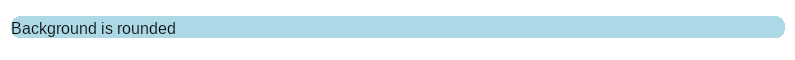
\includegraphics{examples/example11-rounded-background.png}
\caption{Example of a long word with a rounded background.}\label{fig:RoundedCorners}
\end{figure}

%\end{center}

Similar changes should be made to \texttt{InputLayout}. New shapes, like
rounded rectangles, is one way that Skia is a more advanced
rasterization library than Tk. More broadly, since Skia is also used by
Chromium, we know it has fast, built-in support for all of the shapes we
might need in a browser.

\begin{bookblock}{further}
\href{https://en.wikipedia.org/wiki/Font_rasterization}{Font
rasterization} is surprisingly deep, with techniques such as
\href{https://en.wikipedia.org/wiki/Subpixel_rendering}{subpixel
rendering} and
\href{https://en.wikipedia.org/wiki/Font_hinting}{hinting} used to make
fonts look better on lower-resolution screens. These techniques are much
less necessary on
\href{https://en.wikipedia.org/wiki/Pixel_density}{high-pixel-density}
screens, though. It's likely that all screens will eventually be
high-density enough to retire these techniques.
\end{bookblock}

\hypertarget{browser-compositing}{%
\section{Browser Compositing}\label{browser-compositing}}

Skia and SDL have just made our browser more complex, but the low-level
control offered by these libraries is important because it allows us to
optimize common interactions like scrolling.

So far, any time the user scrolled a web page, we had to clear the
canvas and re-raster everything on it from scratch. This is
inefficient---we're drawing the same pixels, just in a different place.
When the context is complex or the screen is large, rastering too often
produces a visible slowdown and drains laptop and mobile batteries. Real
browsers optimize scrolling using a technique I'll call \emph{browser
compositing}: drawing the whole web page to a hidden surface, and only
copying the relevant pixels to the window itself.

To implement this, we'll need two new Skia surfaces: a surface for
browser chrome and a surface for the current \texttt{Tab}'s contents.
We'll only need to re-raster the \texttt{Tab} surface if page contents
change, but not when (say) the user types into the address bar. And we
can scroll the \texttt{Tab} without any raster at all---we just copy a
different part of the current \texttt{Tab} surface to the screen. Let's
call those surfaces \texttt{chrome\_surface} and
\texttt{tab\_surface}:\footnote{We could even use a different surface
  for each \texttt{Tab}, but real browsers don't do this, since each
  surface uses up a lot of memory, and typically users don't notice the
  small raster delay when switching tabs.}
\begin{Shaded}
\begin{Highlighting}[]
\KeywordTok{class}\NormalTok{ Browser:}
    \KeywordTok{def} \FunctionTok{\_\_init\_\_}\NormalTok{(}\VariableTok{self}\NormalTok{):}
        \CommentTok{\# ...}
        \VariableTok{self}\NormalTok{.chrome\_surface }\OperatorTok{=}\NormalTok{ skia.Surface(}
\NormalTok{            WIDTH, math.ceil(}\VariableTok{self}\NormalTok{.chrome.bottom))}
        \VariableTok{self}\NormalTok{.tab\_surface }\OperatorTok{=} \VariableTok{None}
\end{Highlighting}
\end{Shaded}
I'm not explicitly creating \texttt{tab\_surface} right away, because we
need to lay out the page contents to know how tall the surface needs to
be.

We'll also need to split the browser's \texttt{draw} method into three
parts:
\begin{itemize}
\tightlist
\item
  \texttt{raster\_tab} will raster the page to the
  \texttt{tab\_surface};
\item
  \texttt{raster\_chrome} will raster the browser chrome to the
  \texttt{chrome\_surface}; % and
\item
  \texttt{draw} will composite the chrome and tab surfaces and copy the
  result from Skia to SDL.\footnote{It might seem wasteful to copy from
    the chrome and tab surfaces to an intermediate Skia surface, instead
    of directly to the SDL surface. It is, but skipping that copy
    requires a lot of tricky low-level code. In
%    \href{animations.md}{Chapter 13}
    Chapter~\ref{ch:AnimatingAndCompositing} we'll avoid this copy in a
    different, better way.}
\end{itemize}

Let's start by doing the split:
\begin{Shaded}
\begin{Highlighting}[]
\KeywordTok{class}\NormalTok{ Browser:}
    \KeywordTok{def}\NormalTok{ raster\_tab(}\VariableTok{self}\NormalTok{):}
\NormalTok{        canvas }\OperatorTok{=} \VariableTok{self}\NormalTok{.tab\_surface.getCanvas()}
\NormalTok{        canvas.clear(skia.ColorWHITE)}
        \CommentTok{\# ...}

    \KeywordTok{def}\NormalTok{ raster\_chrome(}\VariableTok{self}\NormalTok{):}
\NormalTok{        canvas }\OperatorTok{=} \VariableTok{self}\NormalTok{.chrome\_surface.getCanvas()}
\NormalTok{        canvas.clear(skia.ColorWHITE)}
        \CommentTok{\# ...}

    \KeywordTok{def}\NormalTok{ draw(}\VariableTok{self}\NormalTok{):}
\NormalTok{        canvas }\OperatorTok{=} \VariableTok{self}\NormalTok{.root\_surface.getCanvas()}
\NormalTok{        canvas.clear(skia.ColorWHITE)}
        \CommentTok{\# ...}
\end{Highlighting}
\end{Shaded}
Since we didn't create the \texttt{tab\_surface} on startup, we need to
create it at the top of \texttt{raster\_tab}:\footnote{For a very big
  web page, the \texttt{tab\_surface} can be much larger than the size
  of the SDL window, and therefore take up a very large amount of
  memory. We'll ignore that, but a real browser would only paint and
  raster surface content up to a certain distance from the visible
  region, and re-paint/raster as the user scrolls.}
\begin{Shaded}
\begin{Highlighting}[]
\ImportTok{import}\NormalTok{ math}

\KeywordTok{class}\NormalTok{ Browser:}
    \KeywordTok{def}\NormalTok{ raster\_tab(}\VariableTok{self}\NormalTok{):}
\NormalTok{        tab\_height }\OperatorTok{=}\NormalTok{ math.ceil(}
            \VariableTok{self}\NormalTok{.active\_tab.document.height }\OperatorTok{+} \DecValTok{2}\OperatorTok{*}\NormalTok{VSTEP)}

        \ControlFlowTok{if} \KeywordTok{not} \VariableTok{self}\NormalTok{.tab\_surface }\KeywordTok{or} \OperatorTok{\textbackslash{}}
\NormalTok{                tab\_height }\OperatorTok{!=} \VariableTok{self}\NormalTok{.tab\_surface.height():}
            \VariableTok{self}\NormalTok{.tab\_surface }\OperatorTok{=}\NormalTok{ skia.Surface(WIDTH, tab\_height)}

        \CommentTok{\# ...}
\end{Highlighting}
\end{Shaded}
The way we compute the page bounds here, based on the layout tree's
height, would be incorrect if page elements could stick out below (or to
the right) of their parents---but our browser doesn't support any
features like that. Note that we need to recreate the tab surface if the
page's height changes.

Next, \texttt{draw} should copy from the chrome and tab surfaces to the
root surface. Moreover, we need to translate the \texttt{tab\_surface}
down by \texttt{chrome\_bottom} and up by \texttt{scroll}, and clip it
to % only
just the area of the window that doesn't overlap the browser chrome:
\begin{Shaded}
\begin{Highlighting}[]
\KeywordTok{class}\NormalTok{ Browser:}
    \KeywordTok{def}\NormalTok{ draw(}\VariableTok{self}\NormalTok{):}
        \CommentTok{\# ...}
        
\NormalTok{        tab\_rect }\OperatorTok{=}\NormalTok{ skia.Rect.MakeLTRB(}
            \DecValTok{0}\NormalTok{, }\VariableTok{self}\NormalTok{.chrome.bottom, WIDTH, HEIGHT)}
\NormalTok{        tab\_offset }\OperatorTok{=} \VariableTok{self}\NormalTok{.chrome.bottom }\OperatorTok{{-}} \VariableTok{self}\NormalTok{.active\_tab.scroll}
\NormalTok{        canvas.save()}
\NormalTok{        canvas.clipRect(tab\_rect)}
\NormalTok{        canvas.translate(}\DecValTok{0}\NormalTok{, tab\_offset)}
        \VariableTok{self}\NormalTok{.tab\_surface.draw(canvas, }\DecValTok{0}\NormalTok{, }\DecValTok{0}\NormalTok{)}
\NormalTok{        canvas.restore()}

\NormalTok{        chrome\_rect }\OperatorTok{=}\NormalTok{ skia.Rect.MakeLTRB(}
            \DecValTok{0}\NormalTok{, }\DecValTok{0}\NormalTok{, WIDTH, }\VariableTok{self}\NormalTok{.chrome.bottom)}
\NormalTok{        canvas.save()}
\NormalTok{        canvas.clipRect(chrome\_rect)}
        \VariableTok{self}\NormalTok{.chrome\_surface.draw(canvas, }\DecValTok{0}\NormalTok{, }\DecValTok{0}\NormalTok{)}
\NormalTok{        canvas.restore()}

        \CommentTok{\# ...}
\end{Highlighting}
\end{Shaded}
Note the \texttt{draw} calls: these copy the \texttt{tab\_surface} and
\texttt{chrome\_surface} to the \texttt{canvas}, which is bound to
\texttt{root\_surface}. The \texttt{clipRect} and \texttt{translate}
calls make sure we copy the right parts.

Finally, everywhere in \texttt{Browser} that we call \texttt{draw}, we
now need to call either \texttt{raster\_tab} or \texttt{raster\_chrome}
first. For example, in \texttt{handle\_click}, we do this:
\begin{Shaded}
\begin{Highlighting}[]
\KeywordTok{class}\NormalTok{ Browser:}
    \KeywordTok{def}\NormalTok{ handle\_click(}\VariableTok{self}\NormalTok{, e):}
        \ControlFlowTok{if}\NormalTok{ e.y }\OperatorTok{\textless{}} \VariableTok{self}\NormalTok{.chrome.bottom:}
            \CommentTok{\# ...}
            \VariableTok{self}\NormalTok{.raster\_chrome()}
        \ControlFlowTok{else}\NormalTok{:}
            \CommentTok{\# ...}
            \VariableTok{self}\NormalTok{.raster\_tab()}
        \VariableTok{self}\NormalTok{.draw()}
\end{Highlighting}
\end{Shaded}
Notice how we don't redraw the chrome when only the tab changes, and
vice versa. Likewise, in \texttt{handle\_down}, we don't need to call
\texttt{raster\_tab} at all, since scrolling doesn't change the page.
However, clicking on a web page can cause it to navigate to a new one,
so we do need to detect that and raster the browser chrome if the URL
changed:
\begin{Shaded}
\begin{Highlighting}[]
\KeywordTok{class}\NormalTok{ Browser:}
    \KeywordTok{def}\NormalTok{ handle\_click(}\VariableTok{self}\NormalTok{, e):}
        \ControlFlowTok{if}\NormalTok{ e.y }\OperatorTok{\textless{}} \VariableTok{self}\NormalTok{.chrome.bottom:}
            \CommentTok{\# ...}
        \ControlFlowTok{else}\NormalTok{:}
            \CommentTok{\# ...}
\NormalTok{            url }\OperatorTok{=} \VariableTok{self}\NormalTok{.active\_tab.url}
\NormalTok{            tab\_y }\OperatorTok{=}\NormalTok{ e.y }\OperatorTok{{-}} \VariableTok{self}\NormalTok{.chrome.bottom}
            \VariableTok{self}\NormalTok{.active\_tab.click(e.x, tab\_y)}
            \ControlFlowTok{if} \VariableTok{self}\NormalTok{.active\_tab.url }\OperatorTok{!=}\NormalTok{ url:}
                \VariableTok{self}\NormalTok{.raster\_chrome()}
            \VariableTok{self}\NormalTok{.raster\_tab()}
\end{Highlighting}
\end{Shaded}

We also have some related changes in \texttt{Tab}. Let's rename
\texttt{Tab}'s \texttt{draw} method to \texttt{raster}. In it, we no longer
need to pass around the scroll offset to the \texttt{execute} methods,
or account for \texttt{chrome\_bottom}, because we always draw the whole
tab to the tab surface:
\begin{Shaded}
\begin{Highlighting}[]
\KeywordTok{class}\NormalTok{ Tab:}
    \KeywordTok{def}\NormalTok{ raster(}\VariableTok{self}\NormalTok{, canvas):}
        \ControlFlowTok{for}\NormalTok{ cmd }\KeywordTok{in} \VariableTok{self}\NormalTok{.display\_list:}
\NormalTok{            cmd.execute(canvas)}
\end{Highlighting}
\end{Shaded}
Likewise, we can remove the \texttt{scroll} parameter from each drawing
command's \texttt{execute} method:
\begin{Shaded}
\begin{Highlighting}[]
\KeywordTok{class}\NormalTok{ DrawRect:}
    \KeywordTok{def}\NormalTok{ execute(}\VariableTok{self}\NormalTok{, canvas):}
\NormalTok{        paint }\OperatorTok{=}\NormalTok{ skia.Paint(}
\NormalTok{            Color}\OperatorTok{=}\NormalTok{parse\_color(}\VariableTok{self}\NormalTok{.color),}
\NormalTok{        )}
\NormalTok{        canvas.drawRect(}\VariableTok{self}\NormalTok{.rect, paint)}
\end{Highlighting}
\end{Shaded}

Our browser now uses composited scrolling, making scrolling faster and
smoother, all because we are now using a mix of intermediate surfaces to
store already-rastered content and avoid re-rastering unless the content
has actually changed.

\phantomsection\label{GoFurther:Surfaces}
\begin{bookblock}{further}
Real browsers allocate new surfaces for various different situations,
such as implementing accelerated overflow scrolling and animations of
certain CSS properties such as
\href{https://developer.mozilla.org/en-US/docs/Web/CSS/transform}{transform}
and opacity that can be done without raster. They also allow scrolling
arbitrary HTML elements via
\href{https://developer.mozilla.org/en-US/docs/Web/CSS/overflow}{\texttt{overflow:\ scroll}}
in CSS. Basic scrolling for DOM elements is very similar to what we've
just implemented. But implementing it in its full generality, and with
excellent performance, is \emph{extremely} challenging. Scrolling may
well be the single most complicated feature in a browser rendering
engine. The corner cases and subtleties involved are almost endless.
\end{bookblock}

\hypertarget{transparency}{%
\section{Transparency}\label{transparency}}

Drawing shapes quickly is already a challenge, but with multiple shapes
there's an additional question: what color should the pixel be when two
shapes overlap? So far, our browser has only handled opaque
shapes,\footnote{It also hasn't considered subpixel geometry or
  anti-aliasing, which also rely on color mixing.} and the answer has
been simple: take the color of the top shape. But now we need more
nuance.

Consider partially transparent colors in CSS. These use a hex color with
eight hex digits, with the last two indicating the level of
transparency. For example, the color \texttt{\#00000080} is 50\%
transparent black. Over a white background, that looks gray, but over an
orange background it looks like Figure~\ref{fig:SemitransparentBlack}. %this:
Note that the text is a kind of dark orange, because its color is a mix
of 50\% black and 50\% orange. Many objects in % nature
the real world are partially
transparent: frosted glass, clouds, or colored paper, for example.
Looking through one, you see multiple colors \emph{blended} together.
That's also why computer screens work: the red, green, and blue lights
\href{https://en.wikipedia.org/wiki/Color_mixing}{blend together} and
appear to our eyes as another color. Designers use this
effect\footnote{Mostly. Some more advanced blending modes on the web are
  difficult, or perhaps impossible, in real-world physics.} in overlays,
shadows, and tooltips, so our browser needs to support color mixing.

\begin{figure}[tbp]
\centering

\includegraphics[width=0.8\textwidth]{examples/example11-opacity-blend.png}
\caption{Example of black semi-transparent text blending into an orange
background.}\label{fig:SemitransparentBlack}
\end{figure}

Skia supports this kind of transparency by setting the ``alpha'' field
on the parsed color:
\begin{Shaded}
\begin{Highlighting}[]
\KeywordTok{def}\NormalTok{ parse\_color(color):}
    \CommentTok{\# ...}
    \ControlFlowTok{elif}\NormalTok{ color.startswith(}\StringTok{"\#"}\NormalTok{) }\KeywordTok{and} \BuiltInTok{len}\NormalTok{(color) }\OperatorTok{==} \DecValTok{9}\NormalTok{:}
\NormalTok{        r }\OperatorTok{=} \BuiltInTok{int}\NormalTok{(color[}\DecValTok{1}\NormalTok{:}\DecValTok{3}\NormalTok{], }\DecValTok{16}\NormalTok{)}
\NormalTok{        g }\OperatorTok{=} \BuiltInTok{int}\NormalTok{(color[}\DecValTok{3}\NormalTok{:}\DecValTok{5}\NormalTok{], }\DecValTok{16}\NormalTok{)}
\NormalTok{        b }\OperatorTok{=} \BuiltInTok{int}\NormalTok{(color[}\DecValTok{5}\NormalTok{:}\DecValTok{7}\NormalTok{], }\DecValTok{16}\NormalTok{)}
\NormalTok{        a }\OperatorTok{=} \BuiltInTok{int}\NormalTok{(color[}\DecValTok{7}\NormalTok{:}\DecValTok{9}\NormalTok{], }\DecValTok{16}\NormalTok{)}
        \ControlFlowTok{return}\NormalTok{ skia.Color(r, g, b, a)}
    \CommentTok{\# ...}
\end{Highlighting}
\end{Shaded}
Check that your browser renders dark-orange text for the example above.
That shows that it's actually mixing the black color with the existing
orange color from the background.

However, there's another, subtly different way to create transparency
with CSS. Here, 50\% transparency is applied to the whole element using
the \texttt{opacity} property, as in Figure~\ref{fig:CSSOpacity}.
Now the opacity applies to both the background and the text, so the
background is now a little lighter. But note that the text is now gray,
not dark orange. The black and orange pixels are no longer blended
together!
That's because opacity introduces what CSS calls a
\href{https://developer.mozilla.org/en-US/docs/Web/CSS/CSS_Positioning/Understanding_z_index/The_stacking_context}{stacking
context}. Most of the details aren't important right now, but the order
of operations is. In the first example, the black pixels were first made
transparent, then blended with the background. Thus, 50\% transparent
black pixels were blending with orange pixels, resulting in a
dark-orange color. In the second example, the black pixels were first
blended with the background, then the result was made transparent. Thus,
fully black pixels replaced fully orange ones, resulting in just black
pixels, which were later made 50\% transparent.

\begin{figure}[tbp]
\centering

\includegraphics[width=0.8\textwidth]{examples/example11-text-blending.png}
\caption{Example of black text on an orange background, then blended
semi-transparently into its ancestor.}\label{fig:CSSOpacity}
\end{figure}

Applying blending in the proper order, as is necessary to implement
effects like \texttt{opacity}, requires more careful handling of
surfaces.

\begin{bookblock}{further}
Mostly, elements
\href{https://developer.mozilla.org/en-US/docs/Web/CSS/CSS_Positioning/Understanding_z_index/The_stacking_context}{form
a stacking context} because of CSS properties that have something to do
with layering (like \texttt{z-index}) or visual effects (like
\texttt{mix-blend-mode}). On the other hand, the \texttt{overflow}
property, which can make an element scrollable, does not induce a
stacking context, which I think was a mistake.\footnotemark\ The reason
is that inside a modern browser, scrolling is done on the GPU by
offsetting two surfaces. Without a stacking context the browser might
(depending on the web page structure) have to move around multiple
independent surfaces with complex paint orders, in lockstep, to achieve
scrolling. Fixed- and sticky-positioned elements also form stacking
contexts because of their interaction with scrolling.
\end{bookblock}
\footnotetext{
While we're at
  it, perhaps scrollable elements should also be a
  \href{https://developer.mozilla.org/en-US/docs/Web/CSS/Containing_block}{containing
  block} for descendants. Otherwise, a scrollable element can have
  non-scrolling children via properties like \texttt{position}. This
  situation is very complicated to handle in real browsers.
}

\hypertarget{blending-and-stacking}{%
\section{Blending and Stacking}\label{blending-and-stacking}}

To handle the order of operations properly, browsers apply blending not
to individual shapes but to a tree of surfaces (see Figure~\ref{fig:BlendingSurfaces}).
Conceptually, each shape
is drawn to its own surface, and then blended into its parent surface.
Different structures of intermediate surfaces create different visual
effects.\footnote{You can see a more detailed discussion of how the tree
  structure affects the final image, and how that impacted the CSS
  specifications, on
  \href{https://dbaron.org/log/20130306-compositing-blending}{David
  Baron's blog}.} Rastering a web page requires a bottom-up traversal of
this conceptual tree: to raster a surface you first need to raster its
contents, including its child surfaces, and then the whole contents need
to be blended together into the parent.\footnote{This tree of surfaces
  is an implementation strategy and not something required by any
  specific web API. However, the concept of a
  \href{https://developer.mozilla.org/en-US/docs/Web/CSS/CSS_Positioning/Understanding_z_index/The_stacking_context}{\emph{stacking
  context}} is related. A stacking context is technically a mechanism to
  define groups and ordering during paint, and stacking contexts need
  not correspond to a surface (e.g., ones created via
  \href{https://developer.mozilla.org/en-US/docs/Web/CSS/z-index}{\texttt{z-index}}
  do not). However, for ease of implementation, all visual effects in
  CSS that generally require surfaces to implement are specified to go
  hand-in-hand with a stacking context, so the tree of stacking contexts
  is very related to the tree of surfaces.}

\begin{figure}
\centering
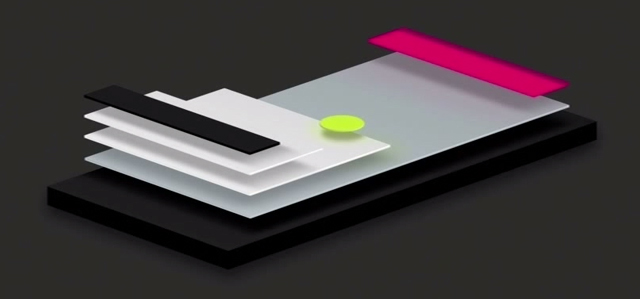
\includegraphics[width=0.9\textwidth]{im/visual-effects-surfaces.jpg}
\caption{A rendered web page is actually the result of stacking and
blending a series of different surfaces.}\label{fig:BlendingSurfaces}
\end{figure}

To match this use pattern, in Skia, surfaces form a stack. You can push
a new surface on the stack, raster things to it, and then pop it off,
which blends it with the surface below. When rastering, you push a new
surface onto the stack every time you need to apply some visual effect,
and pop-and-blend once you're done rastering all the elements that that
effect will be applied to, like this:
\begin{bookblock*}{notcode}
\begin{Shaded}
\begin{Highlighting}[]
\CommentTok{\# draw parent}
\NormalTok{canvas.saveLayer(}\VariableTok{None}\NormalTok{, skia.Paint(Alphaf}\OperatorTok{=}\FloatTok{0.5}\NormalTok{))}
\CommentTok{\# draw children}
\NormalTok{canvas.restore()}
\end{Highlighting}
\end{Shaded}
\end{bookblock*}
\noindent Here, the \texttt{saveLayer} call asks Skia\footnote{It's called
  \texttt{saveLayer} instead of \texttt{createSurface} because Skia
  doesn't actually promise to create a new surface, if it can optimize
  that away. So what you're really doing with \texttt{saveLayer} is
  telling Skia that there is a new conceptual layer (``piece of paper'')
  on the stack. Skia's terminology distinguishes between a layer and a
  surface for this reason as well, but for our purposes it makes sense
  to assume that each new layer comes with a surface.} to draw all the
children to a separate surface before blending them into the parent once
\texttt{restore} is called. The second parameter to
\texttt{saveLayer} specifies the specific type of blending, here with
the \texttt{Alphaf} parameter requesting 50\% opacity.

\texttt{saveLayer} and \texttt{restore} are like a pair of parentheses
enclosing child drawing operations. This means our display list is no
longer just a linear sequence of drawing operations, but a tree. So in
our display list, let's handle \texttt{opacity} with an \texttt{Alpha}
command that takes a sequence of other drawing commands as an argument:
\begin{Shaded}
\begin{Highlighting}[]
\KeywordTok{class}\NormalTok{ Opacity:}
    \KeywordTok{def} \FunctionTok{\_\_init\_\_}\NormalTok{(}\VariableTok{self}\NormalTok{, opacity, children):}
        \VariableTok{self}\NormalTok{.opacity }\OperatorTok{=}\NormalTok{ opacity}
        \VariableTok{self}\NormalTok{.children }\OperatorTok{=}\NormalTok{ children}
        \VariableTok{self}\NormalTok{.rect }\OperatorTok{=}\NormalTok{ skia.Rect.MakeEmpty()}
        \ControlFlowTok{for}\NormalTok{ cmd }\KeywordTok{in} \VariableTok{self}\NormalTok{.children:}
            \VariableTok{self}\NormalTok{.rect.join(cmd.rect)}

    \KeywordTok{def}\NormalTok{ execute(}\VariableTok{self}\NormalTok{, canvas):}
\NormalTok{        paint }\OperatorTok{=}\NormalTok{ skia.Paint(}
\NormalTok{            Alphaf}\OperatorTok{=}\VariableTok{self}\NormalTok{.opacity}
\NormalTok{        )}
\NormalTok{        canvas.saveLayer(paint)}
        \ControlFlowTok{for}\NormalTok{ cmd }\KeywordTok{in} \VariableTok{self}\NormalTok{.children:}
\NormalTok{            cmd.execute(canvas)}
\NormalTok{        canvas.restore()}
\end{Highlighting}
\end{Shaded}
We can now wrap the drawing commands painted by an element with
\texttt{Opacity} to add transparency to the whole element. I'm going to
do this by adding a new \texttt{paint\_effects} method to layout
objects, which should be passed a list of drawing commands to wrap:
\begin{Shaded}
\begin{Highlighting}[]
\KeywordTok{class}\NormalTok{ BlockLayout:}
    \KeywordTok{def}\NormalTok{ paint\_effects(}\VariableTok{self}\NormalTok{, cmds):}
\NormalTok{        cmds }\OperatorTok{=}\NormalTok{ paint\_visual\_effects(}
            \VariableTok{self}\NormalTok{.node, cmds, }\VariableTok{self}\NormalTok{.self\_rect())}
        \ControlFlowTok{return}\NormalTok{ cmds}
\end{Highlighting}
\end{Shaded}
I put the actual construction of the \texttt{Opacity} command in a new
global \texttt{paint\_visual\_effects} method (because other object
types will also need it):
\begin{Shaded}
\begin{Highlighting}[]
\KeywordTok{def}\NormalTok{ paint\_visual\_effects(node, cmds, rect):}
\NormalTok{    opacity }\OperatorTok{=} \BuiltInTok{float}\NormalTok{(node.style.get(}\StringTok{"opacity"}\NormalTok{, }\StringTok{"1.0"}\NormalTok{))}

    \ControlFlowTok{return}\NormalTok{ [}
\NormalTok{        Opacity(opacity, cmds)}
\NormalTok{    ]}
\end{Highlighting}
\end{Shaded}

A change is now needed in \texttt{paint\_tree} to call
\texttt{paint\_effects}, but only \emph{after} recursing into children,
and only if \texttt{should\_paint} is true. That's because these visual
effects apply to the entire subtree's display list, not just the current
object, and don't apply to ``anonymous'' objects (see Chapter~\ref{ch:SendingInformation}). % 8).
\begin{Shaded}
\begin{Highlighting}[]
\KeywordTok{def}\NormalTok{ paint\_tree(layout\_object, display\_list):}
    \ControlFlowTok{if}\NormalTok{ layout\_object.should\_paint():}
\NormalTok{        cmds }\OperatorTok{=}\NormalTok{ layout\_object.paint()}
    \ControlFlowTok{for}\NormalTok{ child }\KeywordTok{in}\NormalTok{ layout\_object.children:}
\NormalTok{        paint\_tree(child, cmds)}

    \ControlFlowTok{if}\NormalTok{ layout\_object.should\_paint():}
\NormalTok{        cmds }\OperatorTok{=}\NormalTok{ layout\_object.paint\_effects(cmds)}
\NormalTok{    display\_list.extend(cmds)}
\end{Highlighting}
\end{Shaded}
Note that \texttt{paint\_visual\_effects} receives a list of commands
and returns another list of commands. It's just that the output list is
always a single \texttt{Opacity} command that wraps the original
content---which makes sense, because first we need to draw the commands
to a surface, and \emph{then} apply transparency to it when blending
into the parent.

\begin{bookblock}{further}
I highly recommend \href{https://ciechanow.ski/alpha-compositing/}{this blog post},
which gives a
really nice visual overview of many of the same concepts explored in
this chapter, plus way more content about how a library such as Skia
might implement features like raster sampling of vector graphics for
lines and text, and interpolation of surfaces when their pixel arrays
don't match in resolution or orientation.
\end{bookblock}

\hypertarget{compositing-pixels}{%
\section{Compositing Pixels}\label{compositing-pixels}}

Now let's pause and explore how opacity actually works under the hood.
Skia, SDL, and many other color libraries account for opacity with a
fourth \emph{alpha} value for each pixel.\footnote{The difference
  between opacity and alpha can be confusing. Think of opacity as a
  visual effect \emph{applied to} content, but alpha as a \emph{part of}
  content. Think of alpha as implementation technique for representing
  opacity.} An alpha of~0 means the pixel is fully transparent (meaning,
no matter what the colors are, you can't see them anyway), and an alpha
of~1 means % a
fully opaque.

When a pixel with alpha overlaps another pixel, the final color is a mix
of their two colors. How exactly the colors are mixed is defined by
Skia's \texttt{Paint} objects. Of course, Skia is pretty complex, but we
can sketch these paint operations in Python as methods on the conceptual
\texttt{Pixel} class I introduced earlier.

When we apply a \texttt{Paint} with an \texttt{Alphaf} parameter, the
first thing Skia does is add the requested opacity to each pixel:
\begin{bookblock*}{notcode}
\begin{Shaded}
\begin{Highlighting}[]
\KeywordTok{class}\NormalTok{ Pixel:}
    \KeywordTok{def}\NormalTok{ alphaf(}\VariableTok{self}\NormalTok{, opacity):}
        \VariableTok{self}\NormalTok{.a }\OperatorTok{=} \VariableTok{self}\NormalTok{.a }\OperatorTok{*}\NormalTok{ opacity}
\end{Highlighting}
\end{Shaded}
\end{bookblock*}
\noindent I want to emphasize that this code is not a part of our browser---I'm
simply using Python code to illustrate what Skia is doing internally.

That \texttt{Alphaf} parameter applies to pixels in one surface. But
with \texttt{saveLayer} we will end up with two surfaces, with all of
their pixels aligned, and therefore we will need to combine, or
\emph{blend}, corresponding pairs of pixels.

Here, the terminology can get confusing: we imagine that the pixels ``on
top'' are blending into the pixels ``below'', so we call the top surface
the \emph{source surface}, with source pixels, and the bottom surface
the \emph{destination surface}, with destination pixels. When we combine
them, there are lots of ways we could do it, but the default on the web
is called ``simple alpha compositing''\index{compositing} or
\emph{source-over} compositing. In Python, the code to implement it
looks like this:\footnote{The formula for this code can be found
  \href{https://www.w3.org/TR/SVG11/masking.html\#SimpleAlphaBlending}{here}.
  Note that that page refers to \emph{premultiplied} alpha colors, but
  Skia's API generally does not use premultiplied representations, and
  this code % below
  doesn't either. (Skia does represent colors internally
  in a premultiplied form, however.)}
\begin{bookblock*}{notcode}
\begin{Shaded}
\begin{Highlighting}[]
\KeywordTok{class}\NormalTok{ Pixel:}
    \KeywordTok{def}\NormalTok{ source\_over(}\VariableTok{self}\NormalTok{, source):}
\NormalTok{        new\_a }\OperatorTok{=}\NormalTok{ source.a }\OperatorTok{+} \VariableTok{self}\NormalTok{.a }\OperatorTok{*}\NormalTok{ (}\DecValTok{1} \OperatorTok{{-}}\NormalTok{ source.a)}
        \ControlFlowTok{if}\NormalTok{ new\_a }\OperatorTok{==} \DecValTok{0}\NormalTok{: }\ControlFlowTok{return} \VariableTok{self}
        \VariableTok{self}\NormalTok{.r }\OperatorTok{=} \OperatorTok{\textbackslash{}}
\NormalTok{            (}\VariableTok{self}\NormalTok{.r }\OperatorTok{*}\NormalTok{ (}\DecValTok{1} \OperatorTok{{-}}\NormalTok{ source.a) }\OperatorTok{*} \VariableTok{self}\NormalTok{.a }\OperatorTok{+} \OperatorTok{\textbackslash{}}
\NormalTok{                source.r }\OperatorTok{*}\NormalTok{ source.a) }\OperatorTok{/}\NormalTok{ new\_a}
        \VariableTok{self}\NormalTok{.g }\OperatorTok{=} \OperatorTok{\textbackslash{}}
\NormalTok{            (}\VariableTok{self}\NormalTok{.g }\OperatorTok{*}\NormalTok{ (}\DecValTok{1} \OperatorTok{{-}}\NormalTok{ source.a) }\OperatorTok{*} \VariableTok{self}\NormalTok{.a }\OperatorTok{+} \OperatorTok{\textbackslash{}}
\NormalTok{                source.g }\OperatorTok{*}\NormalTok{ source.a) }\OperatorTok{/}\NormalTok{ new\_a}
        \VariableTok{self}\NormalTok{.b }\OperatorTok{=} \OperatorTok{\textbackslash{}}
\NormalTok{            (}\VariableTok{self}\NormalTok{.b }\OperatorTok{*}\NormalTok{ (}\DecValTok{1} \OperatorTok{{-}}\NormalTok{ source.a) }\OperatorTok{*} \VariableTok{self}\NormalTok{.a }\OperatorTok{+} \OperatorTok{\textbackslash{}}
\NormalTok{                source.b }\OperatorTok{*}\NormalTok{ source.a) }\OperatorTok{/}\NormalTok{ new\_a}
        \VariableTok{self}\NormalTok{.a }\OperatorTok{=}\NormalTok{ new\_a}
\end{Highlighting}
\end{Shaded}
\end{bookblock*}
\noindent Here, the destination pixel \texttt{self} is modified to blend in the
source pixel \texttt{source}. The mathematical expressions for the red,
green, and blue color channels are identical, and basically average the
source and destination colors, weighted by alpha.\footnote{For example,
  if the alpha of the source pixel is~1, the result is just the source
  pixel color, and if it is~0 the result is the backdrop pixel color.}
You might imagine the overall operation of \texttt{saveLayer} with an
\texttt{Alphaf} parameter as something like this:\footnote{In reality,
  reading individual pixels into memory to manipulate them like this is
  slow, so libraries such as Skia don't make it convenient to do so.
  (Skia canvases do have \texttt{peekPixels} and \texttt{readPixels}
  methods that are sometimes used, but not for this.)}
\begin{bookblock*}{notcode}
\begin{Shaded}
\begin{Highlighting}[]
\ControlFlowTok{for}\NormalTok{ (x, y) }\KeywordTok{in}\NormalTok{ destination.coordinates():}
\NormalTok{    source[x, y].alphaf(opacity)}
\NormalTok{    destination[x, y].source\_over(source[x, y])}
\end{Highlighting}
\end{Shaded}
\end{bookblock*}

Source-over compositing is one way to combine two pixel values. But it's
not the only method---you could write literally any computation that
combines two pixel values if you wanted. Two computations that produce
interesting effects are traditionally called ``multiply'' and
``difference'' and use simple mathematical operations. ``Multiply''
multiplies the color values:
\begin{bookblock*}{notcode}
\begin{Shaded}
\begin{Highlighting}[]
\KeywordTok{class}\NormalTok{ Pixel:}
    \KeywordTok{def}\NormalTok{ multiply(}\VariableTok{self}\NormalTok{, source):}
        \VariableTok{self}\NormalTok{.r }\OperatorTok{=} \VariableTok{self}\NormalTok{.r }\OperatorTok{*}\NormalTok{ source.r}
        \VariableTok{self}\NormalTok{.g }\OperatorTok{=} \VariableTok{self}\NormalTok{.g }\OperatorTok{*}\NormalTok{ source.g}
        \VariableTok{self}\NormalTok{.b }\OperatorTok{=} \VariableTok{self}\NormalTok{.b }\OperatorTok{*}\NormalTok{ source.b}
\end{Highlighting}
\end{Shaded}
\end{bookblock*}
\noindent And ``difference'' computes their absolute differences:
\begin{bookblock*}{notcode}
\begin{Shaded}
\begin{Highlighting}[]
\KeywordTok{class}\NormalTok{ Pixel:}
    \KeywordTok{def}\NormalTok{ difference(}\VariableTok{self}\NormalTok{, source):}
        \VariableTok{self}\NormalTok{.r }\OperatorTok{=} \BuiltInTok{abs}\NormalTok{(}\VariableTok{self}\NormalTok{.r }\OperatorTok{{-}}\NormalTok{ source.r)}
        \VariableTok{self}\NormalTok{.g }\OperatorTok{=} \BuiltInTok{abs}\NormalTok{(}\VariableTok{self}\NormalTok{.g }\OperatorTok{{-}}\NormalTok{ source.g)}
        \VariableTok{self}\NormalTok{.b }\OperatorTok{=} \BuiltInTok{abs}\NormalTok{(}\VariableTok{self}\NormalTok{.b }\OperatorTok{{-}}\NormalTok{ source.b)}
\end{Highlighting}
\end{Shaded}
\end{bookblock*}

CSS supports these and many other blending modes\footnote{Many of these
  blending modes are
  \href{https://en.wikipedia.org/wiki/Blend_modes}{common} to other
  graphics editing programs like Photoshop and GIMP. Some, like
  \href{https://en.wikipedia.org/wiki/Dodging_and_burning}{``dodge'' and
  ``burn''}, go back to analog photography, where photographers would
  expose some parts of the image more than others to manipulate their
  brightness.} via the
\href{https://drafts.fxtf.org/compositing-1/\#propdef-mix-blend-mode}{\texttt{mix-blend-mode}
property}, like this:
{\small%
\begin{bookblock*}{notcode}
\begin{Shaded}
\begin{Highlighting}[]
\KeywordTok{\textless{}div} \ErrorTok{style}\OtherTok{=}\StringTok{"background{-}color:orange"}\KeywordTok{\textgreater{}}
\NormalTok{    Parent}
    \KeywordTok{\textless{}div} \ErrorTok{style}\OtherTok{=}\StringTok{"background{-}color:blue;mix{-}blend{-}mode:difference"}\KeywordTok{\textgreater{}}
\NormalTok{        Child}
    \KeywordTok{\textless{}/div\textgreater{}}
\NormalTok{    Parent}
\KeywordTok{\textless{}/div\textgreater{}}
\end{Highlighting}
\end{Shaded}
\end{bookblock*}}
\noindent This HTML will look like Figure~\ref{fig:DifferenceMix}.
Here, when blue overlaps with orange, we see pink: blue has (red, green,
blue) color channels of \texttt{(0,\ 0,\ 1)}, and orange has
\texttt{(1,\ 0.65,\ 0)}, so with ``difference'' blending the resulting
pixel will be \texttt{(1,\ 0.65,\ 1)}, which is pink. On a pixel level,
what's happening is something like this:
\begin{bookblock*}{notcode}
\begin{Shaded}
\begin{Highlighting}[]
\ControlFlowTok{for}\NormalTok{ (x, y) }\KeywordTok{in}\NormalTok{ destination.coordinates():}
\NormalTok{    source[x, y].alphaf(opacity)}
\NormalTok{    source[x, y].difference(destination[x, y])}
\NormalTok{    destination[x, y].source\_over(source[x, y])}
\end{Highlighting}
\end{Shaded}
\end{bookblock*}
\noindent This looks weird, but conceptually it blends the destination into the
source (which ignores alpha) and then draws the source over the
destination (with alpha considered). In some sense, blending thus
\href{https://drafts.fxtf.org/compositing-1/\#blending}{happens twice}.

\begin{figure}[tbp]
\centering
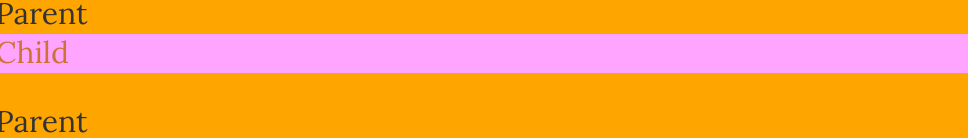
\includegraphics[width=0.9\textwidth]{examples/example11-difference-blend-mode.png}
\caption{Example of the \texttt{difference} value for
\texttt{mix-blend-mode} with a blue child and orange parent, resulting
in pink.}\label{fig:DifferenceMix}
\end{figure}

Skia supports the
\href{https://drafts.fxtf.org/compositing-1/\#blendingmultiply}{multiply}
and
\href{https://drafts.fxtf.org/compositing-1/\#blendingdifference}{difference}
blend modes natively:
\begin{Shaded}
\begin{Highlighting}[]
\KeywordTok{def}\NormalTok{ parse\_blend\_mode(blend\_mode\_str):}
    \ControlFlowTok{if}\NormalTok{ blend\_mode\_str }\OperatorTok{==} \StringTok{"multiply"}\NormalTok{:}
        \ControlFlowTok{return}\NormalTok{ skia.BlendMode.kMultiply}
    \ControlFlowTok{elif}\NormalTok{ blend\_mode\_str }\OperatorTok{==} \StringTok{"difference"}\NormalTok{:}
        \ControlFlowTok{return}\NormalTok{ skia.BlendMode.kDifference}
    \ControlFlowTok{else}\NormalTok{:}
        \ControlFlowTok{return}\NormalTok{ skia.BlendMode.kSrcOver}
\end{Highlighting}
\end{Shaded}
We can then support blending in our browser by defining a new
\texttt{Blend} operation:
\begin{Shaded}
\begin{Highlighting}[]
\KeywordTok{class}\NormalTok{ Blend:}
    \KeywordTok{def} \FunctionTok{\_\_init\_\_}\NormalTok{(}\VariableTok{self}\NormalTok{, blend\_mode, children):}
        \VariableTok{self}\NormalTok{.blend\_mode }\OperatorTok{=}\NormalTok{ blend\_mode}

        \VariableTok{self}\NormalTok{.children }\OperatorTok{=}\NormalTok{ children}
        \VariableTok{self}\NormalTok{.rect }\OperatorTok{=}\NormalTok{ skia.Rect.MakeEmpty()}
        \ControlFlowTok{for}\NormalTok{ cmd }\KeywordTok{in} \VariableTok{self}\NormalTok{.children:}
            \VariableTok{self}\NormalTok{.rect.join(cmd.rect)}

    \KeywordTok{def}\NormalTok{ execute(}\VariableTok{self}\NormalTok{, canvas):}
\NormalTok{        paint }\OperatorTok{=}\NormalTok{ skia.Paint(}
\NormalTok{            BlendMode}\OperatorTok{=}\NormalTok{parse\_blend\_mode(}\VariableTok{self}\NormalTok{.blend\_mode),}
\NormalTok{        )}
\NormalTok{        canvas.saveLayer(}\VariableTok{None}\NormalTok{, paint)}
        \ControlFlowTok{for}\NormalTok{ cmd }\KeywordTok{in} \VariableTok{self}\NormalTok{.children:}
\NormalTok{            cmd.execute(canvas)}
\NormalTok{        canvas.restore()}
\end{Highlighting}
\end{Shaded}

Applying it when \texttt{mix-blend-mode} is set just requires a simple
change to \texttt{paint\_visual\_effects}:
\begin{Shaded}
\begin{Highlighting}[]
\KeywordTok{def}\NormalTok{ paint\_visual\_effects(node, cmds, rect):}
    \CommentTok{\# ...}
\NormalTok{    blend\_mode }\OperatorTok{=}\NormalTok{ node.style.get(}\StringTok{"mix{-}blend{-}mode"}\NormalTok{)}
    
    \ControlFlowTok{return}\NormalTok{ [}
\NormalTok{        Blend(blend\_mode, [}
\NormalTok{            Opacity(opacity, cmds),}
\NormalTok{        ]),}
\NormalTok{    ]}
\end{Highlighting}
\end{Shaded}
Note the order of operations here: we \emph{first} apply transparency,
and \emph{then} blend the result into the rest of the page. If we
switched the \texttt{Opacity} and \texttt{Blend} calls there wouldn't be
anything to blend it into!

\begin{bookblock}{further}
Alpha might seem intuitive, but it's less obvious than you think: see,
for example, this
\href{http://alvyray.com/Memos/CG/Microsoft/7_alpha.pdf}{history of
alpha} written by its co-inventor (and co-founder of Pixar). And there
are several different implementation options. For example, many graphics
libraries, Skia included, multiply the color channels by the opacity
instead of allocating a whole color channel. This
\href{https://limnu.com/premultiplied-alpha-primer-artists/}{premultiplied}
representation is generally more efficient; for example,
\texttt{source\_over} above had to divide by \texttt{self.a} at the end,
because otherwise the result would be premultiplied. Using a
premultiplied representation throughout would save a division. Nor is it
obvious how alpha
\href{https://jcgt.org/published/0004/02/03/paper.pdf}{behaves when
resized}.
\end{bookblock}

\hypertarget{clipping-and-masking}{%
\section{Clipping and Masking}\label{clipping-and-masking}}

The ``multiply'' and ``difference'' blend modes can seem kind of
obscure, but blend modes are a flexible way to implement per-pixel
operations. One common use case is clipping---intersecting a surface
with a given shape. It's called clipping because it's like putting a
second piece of paper (called a \emph{mask}) over the first one, and
then using scissors to cut along the mask's edge.

There are all sorts of powerful methods\footnote{The CSS
  \href{https://developer.mozilla.org/en-US/docs/Web/CSS/clip-path}{\texttt{clip-path}
  property} lets you specify a mask shape using a curve, while the
  \href{https://developer.mozilla.org/en-US/docs/Web/CSS/mask}{\texttt{mask}
  property} lets you instead specify a image URL for the mask.} for
clipping content on the web, but the most common form involves the
\texttt{overflow} property. This property has lots of possible
values,\footnote{For example, \texttt{overflow:\ scroll} adds scroll
  bars and makes an element scrollable, while \texttt{overflow:\ hidden}
  is similar to but subtly different from \texttt{overflow:\ clip}.} but
let's focus here on \texttt{overflow:\ clip}, which cuts off contents of
an element that are outside the element's bounds.

\begin{figure}[btp]
\centering
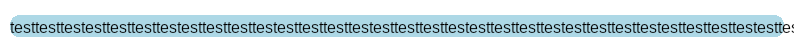
\includegraphics{examples/example11-longword.png}
\caption{An example of overflowing text not being clipped by rounded
corners.}\label{longword-example}
\end{figure}

Usually, \texttt{overflow:\ clip} is used with properties like
\texttt{height} or \texttt{rotate} which can make an element's children
poke outside their parent. Our browser doesn't support these, but there
is one edge case where \texttt{overflow:\ clip} is relevant: rounded
corners.\footnote{Technically, clipping is also relevant for our browser
  with single words that are longer than the browser window's width. See
  Figure~\ref{longword-example} for an example.} Consider this example:
{\small%
  \begin{bookblock*}{notcode}
\begin{Shaded}
\begin{Highlighting}[]
\DataTypeTok{\textless{}}\KeywordTok{div}\OtherTok{ }
\OtherTok{  style}\OperatorTok{=}\StringTok{"border{-}radius:30px;background{-}color:lightblue;overflow:clip"}\DataTypeTok{\textgreater{}}
\NormalTok{    This test text exists here to ensure that the "div" element is}
\NormalTok{    large enough that the border radius is obvious.}
\DataTypeTok{\textless{}/}\KeywordTok{div}\DataTypeTok{\textgreater{}}
\end{Highlighting}
\end{Shaded}
\end{bookblock*}}
\noindent That HTML looks like Figure~\ref{fig:OverflowClip}. % this:
Observe that the letters near the corner are cut off to maintain a sharp
rounded edge. That's clipping; without the \texttt{overflow:\ clip}
property these letters would instead be fully drawn, like we saw % earlier in this chapter
in Figure~\ref{fig:RoundedCorners}.

\begin{figure}[tbp]
\centering
\includegraphics[width=0.9\textwidth]{examples/example11-overflow-clip.png}
\caption{An example of overflow from text children of a \texttt{div} with
\texttt{overflow:clip} and \texttt{border-radius} being clipped out.}\label{fig:OverflowClip}
\end{figure}

Counterintuitively, we'll implement clipping using blending modes. We'll
make a new surface (the mask), draw a rounded rectangle into it, and
then blend it with the element contents. But we want to see the element
contents, not the mask, so when we do this blending we will use
\emph{destination-in} compositing.
\href{https://drafts.fxtf.org/compositing-1/\#porterduffcompositingoperators_dstin}{Destination-in
compositing} basically means keeping the pixels of the destination
surface that intersect with the source surface. The source surface's
color is not used---just its alpha. In our case, the source surface is
the rounded rectangle mask and the destination surface is the content we
want to clip, so destination-in fits perfectly. In code, destination-in
looks like this:
\begin{bookblock*}{notcode}
\begin{Shaded}
\begin{Highlighting}[]
\KeywordTok{class}\NormalTok{ Pixel:}
    \KeywordTok{def}\NormalTok{ destination\_in(}\VariableTok{self}\NormalTok{, source):}
        \VariableTok{self}\NormalTok{.a }\OperatorTok{=} \VariableTok{self}\NormalTok{.a }\OperatorTok{*}\NormalTok{ source.a}
\end{Highlighting}
\end{Shaded}
\end{bookblock*}

Now, in \texttt{paint\_visual\_effects}, we need to create a new layer,
draw the mask image into it, and then blend it with the element contents
with destination-in blending:
\begin{Shaded}
\begin{Highlighting}[]
\KeywordTok{def}\NormalTok{ paint\_visual\_effects(node, cmds, rect):}
    \CommentTok{\# ...}
    \ControlFlowTok{if}\NormalTok{ node.style.get(}\StringTok{"overflow"}\NormalTok{, }\StringTok{"visible"}\NormalTok{) }\OperatorTok{==} \StringTok{"clip"}\NormalTok{:}
\NormalTok{        border\_radius }\OperatorTok{=} \BuiltInTok{float}\NormalTok{(node.style.get(}
            \StringTok{"border{-}radius"}\NormalTok{, }\StringTok{"0px"}\NormalTok{)[:}\OperatorTok{{-}}\DecValTok{2}\NormalTok{])}
\NormalTok{        cmds.append(Blend(}\StringTok{"destination{-}in"}\NormalTok{, [}
\NormalTok{            DrawRRect(rect, border\_radius, }\StringTok{"white"}\NormalTok{)}
\NormalTok{        ]))}

    \ControlFlowTok{return}\NormalTok{ [}
\NormalTok{        Blend(blend\_mode, [}
\NormalTok{            Opacity(opacity, cmds),}
\NormalTok{        ]),}
\NormalTok{    ]}
\end{Highlighting}
\end{Shaded}
Here I pass \texttt{destination-in} as the blend mode, though note that
this is a bit of a hack and that isn't actually a valid value of
\texttt{mix-blend-mode}:
\begin{Shaded}
\begin{Highlighting}[]
\KeywordTok{def}\NormalTok{ parse\_blend\_mode(blend\_mode\_str):}
    \CommentTok{\# ...}
    \ControlFlowTok{elif}\NormalTok{ blend\_mode\_str }\OperatorTok{==} \StringTok{"destination{-}in"}\NormalTok{:}
        \ControlFlowTok{return}\NormalTok{ skia.BlendMode.kDstIn}
    \CommentTok{\# ...}
\end{Highlighting}
\end{Shaded}
After drawing all of the element contents with \texttt{cmds} (and
applying opacity), this code draws a rounded rectangle on another layer
to serve as the mask, and uses destination-in blending to clip the
element contents. Here I chose to draw the rounded rectangle in white,
but the color doesn't matter as long as it's opaque. On the other hand,
if there's no clipping, I don't round the corners of the mask, which
means nothing is clipped out.

Notice how similar this masking technique is to the physical analogy
with scissors described earlier, with the two layers playing the role of
two sheets of paper and destination-in compositing playing the role of
the scissors.\footnote{If all our browser wanted to clip were rounded
  rectangles, Skia actually provides a specialized \texttt{clipRRect}
  operation. It's more efficient than destination-in blending because it
  applies as other commands are being drawn, and so can skip drawing
  anything outside the clipped region. This requires specialized code in
  each of Skia's \emph{shaders}, or GPU programs, so can only be done
  for a couple of common shapes. Destination-in blending is more
  general.}

\begin{bookblock}{further}
Rounded corners have an
\href{https://www.folklore.org/StoryView.py?story=Round_Rects_Are_Everywhere.txt}{interesting
history} in computing. Features that are simple today were
\href{https://raw.githubusercontent.com/jrk/QuickDraw/master/RRects.a}{very
complex} to implement on early personal computers with limited memory
and no hardware floating-point arithmetic. Even when floating-point
hardware and eventually GPUs became standard, the \texttt{border-radius}
CSS property didn't appear in browsers until around 2010.\footnotemark\ More recently, the introduction of
animations, visual effects, multi-process compositing, and
\href{https://en.wikipedia.org/wiki/Hardware_overlay}{hardware overlays}
have made rounded corners pretty complex to implement. The
\texttt{clipRRect} fast path, for example, can fail to apply for cases
such as hardware video overlays and nested rounded corner clips.
\end{bookblock}
\footnotetext{
The lack of support didn't stop web developers from putting rounded
  corners on their sites before \texttt{border-radius} was supported.
  There are a number of clever ways to do it;
  \href{https://css-tricks.com/video-screencasts/24-rounded-corners/}{this
  video} walks through several.
}

\hypertarget{optimizing-surface-use}{%
\section{Optimizing Surface Use}\label{optimizing-surface-use}}

Our browser now works correctly, but uses way too many surfaces. For
example, for a single, no-effects-needed \texttt{div} with some text content,
there are currently 18 surfaces allocated in the display list. If
there's no blending going on, we should only need one!

Let's review all the surfaces that our code can create for an element:
\begin{itemize}
%\tightlist
\item
  The top-level surface is used to apply \emph{blend modes}. Since it's
  the top-level surface, it also \emph{isolates} the element from other
  parts of the page, so that clipping only applies to that element.
\item
  The first nested surface is used for applying \emph{opacity}.
\item
  The second nested surface is used to implement \emph{clipping}.
\end{itemize}
But not every element has opacity, blend modes, or clipping applied, and
we could skip creating those surfaces most of the time. For example,
there's no reason to create a surface in \texttt{Opacity} if no opacity
is actually applied:
\begin{Shaded}
\begin{Highlighting}[]
\KeywordTok{class}\NormalTok{ Opacity:}
    \KeywordTok{def}\NormalTok{ execute(}\VariableTok{self}\NormalTok{, canvas):}
\NormalTok{        paint }\OperatorTok{=}\NormalTok{ skia.Paint(}
\NormalTok{            Alphaf}\OperatorTok{=}\VariableTok{self}\NormalTok{.opacity,}
\NormalTok{        )}
        \ControlFlowTok{if} \VariableTok{self}\NormalTok{.opacity }\OperatorTok{\textless{}} \DecValTok{1}\NormalTok{:}
\NormalTok{            canvas.saveLayer(}\VariableTok{None}\NormalTok{, paint)}
        \ControlFlowTok{for}\NormalTok{ cmd }\KeywordTok{in} \VariableTok{self}\NormalTok{.children:}
\NormalTok{            cmd.execute(canvas)}
        \ControlFlowTok{if} \VariableTok{self}\NormalTok{.opacity }\OperatorTok{\textless{}} \DecValTok{1}\NormalTok{:}
\NormalTok{            canvas.restore()}
\end{Highlighting}
\end{Shaded}

Similarly, \texttt{Blend} doesn't necessarily need to create a layer if
there's no blending going on. But the logic here is a little trickier: the
\texttt{Blend} operation not only applies blending but also isolates the
element contents \texttt{cmds}, which matters if they are being clipped
by \texttt{overflow}. So let's skip creating a layer in \texttt{Blend}
when there's no blending mode, but let's set the blend mode to a
special, non-standard \texttt{source-over} value when we need clipping:
\begin{Shaded}
\begin{Highlighting}[]
\KeywordTok{def}\NormalTok{ paint\_visual\_effects(node, cmds, rect):}
    \ControlFlowTok{if}\NormalTok{ node.style.get(}\StringTok{"overflow"}\NormalTok{, }\StringTok{"visible"}\NormalTok{) }\OperatorTok{==} \StringTok{"clip"}\NormalTok{:}
        \ControlFlowTok{if} \KeywordTok{not}\NormalTok{ blend\_mode:}
\NormalTok{            blend\_mode }\OperatorTok{=} \StringTok{"source{-}over"}
        \CommentTok{\# ...}
\end{Highlighting}
\end{Shaded}
We'll parse that as the default source-over blend mode:
\begin{Shaded}
\begin{Highlighting}[]
\KeywordTok{def}\NormalTok{ parse\_blend\_mode(blend\_mode\_str):}
    \CommentTok{\# ...}
    \ControlFlowTok{elif}\NormalTok{ blend\_mode\_str }\OperatorTok{==} \StringTok{"source{-}over"}\NormalTok{:}
        \ControlFlowTok{return}\NormalTok{ skia.BlendMode.kSrcOver}
    \CommentTok{\# ...}
\end{Highlighting}
\end{Shaded}
This is actually unnecessary, since \texttt{parse\_blend\_mode} already
parses unknown strings as source-over blending, but it's good to be
explicit. Anyway, now \texttt{Blend} can skip \texttt{saveLayer} if no
blend mode is passed:
\begin{Shaded}
\begin{Highlighting}[]
\KeywordTok{class}\NormalTok{ Blend:}
    \KeywordTok{def}\NormalTok{ execute(}\VariableTok{self}\NormalTok{, canvas):}
\NormalTok{        paint }\OperatorTok{=}\NormalTok{ skia.Paint(}
\NormalTok{            BlendMode}\OperatorTok{=}\NormalTok{parse\_blend\_mode(}\VariableTok{self}\NormalTok{.blend\_mode),}
\NormalTok{        )}
        \ControlFlowTok{if} \VariableTok{self}\NormalTok{.blend\_mode:}
\NormalTok{            canvas.saveLayer(}\VariableTok{None}\NormalTok{, paint)}
        \ControlFlowTok{for}\NormalTok{ cmd }\KeywordTok{in} \VariableTok{self}\NormalTok{.children:}
\NormalTok{            cmd.execute(canvas)}
        \ControlFlowTok{if} \VariableTok{self}\NormalTok{.blend\_mode:}
\NormalTok{            canvas.restore()}
\end{Highlighting}
\end{Shaded}

So now we skip creating extra surfaces when \texttt{Opacity} and
\texttt{Blend} aren't really necessary. But there's still one case where
we use too many: both \texttt{Opacity} and \texttt{Blend} can create a
surface instead of sharing one. Let's fix that by just merging opacity
into \texttt{Blend}:\footnote{This works for opacity, but not for
  filters that ``move pixels'' such as
  \href{https://developer.mozilla.org/en-US/docs/Web/CSS/filter-function/blur()}{blur}.
  Such a filter needs to be applied before clipping, not when blending
  into the parent surface. Otherwise, the edge of the blur will not be
  sharp.}
\begin{Shaded}
\begin{Highlighting}[]
\KeywordTok{class}\NormalTok{ Blend:}
    \KeywordTok{def} \FunctionTok{\_\_init\_\_}\NormalTok{(}\VariableTok{self}\NormalTok{, opacity, blend\_mode, children):}
        \VariableTok{self}\NormalTok{.opacity }\OperatorTok{=}\NormalTok{ opacity}
        \VariableTok{self}\NormalTok{.blend\_mode }\OperatorTok{=}\NormalTok{ blend\_mode}
        \VariableTok{self}\NormalTok{.should\_save }\OperatorTok{=} \VariableTok{self}\NormalTok{.blend\_mode }\KeywordTok{or} \VariableTok{self}\NormalTok{.opacity }\OperatorTok{\textless{}} \DecValTok{1}

        \VariableTok{self}\NormalTok{.children }\OperatorTok{=}\NormalTok{ children}
        \VariableTok{self}\NormalTok{.rect }\OperatorTok{=}\NormalTok{ skia.Rect.MakeEmpty()}
        \ControlFlowTok{for}\NormalTok{ cmd }\KeywordTok{in} \VariableTok{self}\NormalTok{.children:}
            \VariableTok{self}\NormalTok{.rect.join(cmd.rect)}


    \KeywordTok{def}\NormalTok{ execute(}\VariableTok{self}\NormalTok{, canvas):}
\NormalTok{        paint }\OperatorTok{=}\NormalTok{ skia.Paint(}
\NormalTok{            Alphaf}\OperatorTok{=}\VariableTok{self}\NormalTok{.opacity,}
\NormalTok{            BlendMode}\OperatorTok{=}\NormalTok{parse\_blend\_mode(}\VariableTok{self}\NormalTok{.blend\_mode),}
\NormalTok{        )}
        \ControlFlowTok{if} \VariableTok{self}\NormalTok{.should\_save:}
\NormalTok{            canvas.saveLayer(}\VariableTok{None}\NormalTok{, paint)}
        \ControlFlowTok{for}\NormalTok{ cmd }\KeywordTok{in} \VariableTok{self}\NormalTok{.children:}
\NormalTok{            cmd.execute(canvas)}
        \ControlFlowTok{if} \VariableTok{self}\NormalTok{.should\_save:}
\NormalTok{            canvas.restore()}
\end{Highlighting}
\end{Shaded}
Now \texttt{paint\_visual\_effects} looks like this:
\begin{Shaded}
\begin{Highlighting}[]
\KeywordTok{def}\NormalTok{ paint\_visual\_effects(node, cmds, rect):}
    \CommentTok{\# ...}

    \ControlFlowTok{if}\NormalTok{ node.style.get(}\StringTok{"overflow"}\NormalTok{, }\StringTok{"visible"}\NormalTok{) }\OperatorTok{==} \StringTok{"clip"}\NormalTok{:}
        \CommentTok{\# ...}
\NormalTok{        cmds.append(Blend(}\FloatTok{1.0}\NormalTok{, }\StringTok{"destination{-}in"}\NormalTok{, [}
\NormalTok{            DrawRRect(rect, border\_radius, }\StringTok{"white"}\NormalTok{)}
\NormalTok{        ]))}

    \ControlFlowTok{return}\NormalTok{ [Blend(opacity, blend\_mode, cmds)]}
\end{Highlighting}
\end{Shaded}
Note that I've specified an opacity of \texttt{1.0} for the clip
\texttt{Blend}.

\begin{bookblock}{further}
Implementing high-quality raster libraries is very interesting in its
own right---check out
\href{https://www.realtimerendering.com/}{Real-Time Rendering} for
more.\footnotemark\ These days, it's especially
important to leverage GPUs when they're available, and browsers often
push the envelope. Browser teams typically include or work closely with
raster library experts: Skia for Chromium and
\href{https://developer.apple.com/documentation/coregraphics}{Core
Graphics} for WebKit, for example. Both of these libraries are used
outside of the browser, too: Core Graphics in iOS and macOS, and Skia in
Android.
\end{bookblock}
\footnotetext{
There is also
  \href{https://en.wikipedia.org/wiki/Computer_Graphics:_Principles_and_Practice}{Computer
  Graphics: Principles and Practice}, which incidentally I remember
  buying---this is Chris speaking---back in the days of my youth (1992
  or so). At the time I didn't get much further than rastering lines and
  polygons (in assembly language!). These days you can do the same and
  more with Skia and a few lines of Python.
}

\hypertarget{summary}{%
\section{Summary}\label{VisualEffects-summary}}

So there you have it: our browser can draw not only boring text and
boxes but also:
\begin{itemize}
%\tightlist
\item
  partial transparency via an alpha channel;
\item
  user-configurable blending modes via \texttt{mix-blend-mode};
\item
  rounded rectangle clipping via destination-in blending or direct
  clipping;
\item
  optimizations to avoid surfaces when possible;
\item
  browser compositing with extra surfaces for faster scrolling.
\end{itemize}
Besides the new features, we've upgraded from Tkinter to SDL and Skia,
which makes our browser faster and more responsive, and also sets a
foundation for more work on browser performance to come.

\hypertarget{outline}{%
\section{Outline}\label{VisualEffects-outline}}

The complete set of functions, classes, and methods in our browser
should now look something like this:
\begin{Shaded}
\begin{Highlighting}[]
\NormalTok{WIDTH}
\NormalTok{HEIGHT}
\NormalTok{HSTEP}
\NormalTok{VSTEP}
\NormalTok{SCROLL\_STEP}
\KeywordTok{def}\NormalTok{ print\_tree(node, indent)}
\KeywordTok{class}\NormalTok{ HTMLParser:}
    \KeywordTok{def} \FunctionTok{\_\_init\_\_}\NormalTok{(body)}
    \KeywordTok{def}\NormalTok{ parse()}
    \KeywordTok{def}\NormalTok{ get\_attributes(text)}
    \KeywordTok{def}\NormalTok{ add\_text(text)}
\NormalTok{    SELF\_CLOSING\_TAGS}
    \KeywordTok{def}\NormalTok{ add\_tag(tag)}
\NormalTok{    HEAD\_TAGS}
    \KeywordTok{def}\NormalTok{ implicit\_tags(tag)}
    \KeywordTok{def}\NormalTok{ finish()}
\NormalTok{BLOCK\_ELEMENTS}
\KeywordTok{class}\NormalTok{ CSSParser:}
    \KeywordTok{def} \FunctionTok{\_\_init\_\_}\NormalTok{(s)}
    \KeywordTok{def}\NormalTok{ whitespace()}
    \KeywordTok{def}\NormalTok{ literal(literal)}
    \KeywordTok{def}\NormalTok{ word()}
    \KeywordTok{def}\NormalTok{ pair()}
    \KeywordTok{def}\NormalTok{ ignore\_until(chars)}
    \KeywordTok{def}\NormalTok{ body()}
    \KeywordTok{def}\NormalTok{ selector()}
    \KeywordTok{def}\NormalTok{ parse()}
\KeywordTok{class}\NormalTok{ TagSelector:}
    \KeywordTok{def} \FunctionTok{\_\_init\_\_}\NormalTok{(tag)}
    \KeywordTok{def}\NormalTok{ matches(node)}
\KeywordTok{class}\NormalTok{ DescendantSelector:}
    \KeywordTok{def} \FunctionTok{\_\_init\_\_}\NormalTok{(ancestor, descendant)}
    \KeywordTok{def}\NormalTok{ matches(node)}
\NormalTok{INHERITED\_PROPERTIES}
\KeywordTok{def}\NormalTok{ style(node, rules)}
\KeywordTok{def}\NormalTok{ cascade\_priority(rule)}
\KeywordTok{class}\NormalTok{ DrawText:}
    \KeywordTok{def} \FunctionTok{\_\_init\_\_}\NormalTok{(x1, y1, text, font, color)}
    \KeywordTok{def}\NormalTok{ execute(canvas)}
\KeywordTok{def}\NormalTok{ tree\_to\_list(tree, }\NormalTok{list}\NormalTok{)}
\KeywordTok{class}\NormalTok{ DrawLine:}
    \KeywordTok{def} \FunctionTok{\_\_init\_\_}\NormalTok{(x1, y1, x2, y2, color, thickness)}
    \KeywordTok{def}\NormalTok{ execute(canvas)}
\KeywordTok{class}\NormalTok{ DrawOutline:}
    \KeywordTok{def} \FunctionTok{\_\_init\_\_}\NormalTok{(rect, color, thickness)}
    \KeywordTok{def}\NormalTok{ execute(canvas)}
\KeywordTok{class}\NormalTok{ DrawRect:}
    \KeywordTok{def} \FunctionTok{\_\_init\_\_}\NormalTok{(rect, color)}
    \KeywordTok{def}\NormalTok{ execute(canvas)}
\KeywordTok{class}\NormalTok{ Text:}
    \KeywordTok{def} \FunctionTok{\_\_init\_\_}\NormalTok{(text, parent)}
    \KeywordTok{def} \FunctionTok{\_\_repr\_\_}\NormalTok{()}
\KeywordTok{class}\NormalTok{ Element:}
    \KeywordTok{def} \FunctionTok{\_\_init\_\_}\NormalTok{(tag, attributes, parent)}
    \KeywordTok{def} \FunctionTok{\_\_repr\_\_}\NormalTok{()}
\KeywordTok{class}\NormalTok{ BlockLayout:}
    \KeywordTok{def} \FunctionTok{\_\_init\_\_}\NormalTok{(node, parent, previous)}
    \KeywordTok{def}\NormalTok{ token(tok)}
    \KeywordTok{def}\NormalTok{ word(node, word)}
    \KeywordTok{def}\NormalTok{ flush()}
    \KeywordTok{def}\NormalTok{ recurse(node)}
    \KeywordTok{def}\NormalTok{ layout()}
    \KeywordTok{def}\NormalTok{ layout\_mode()}
    \KeywordTok{def}\NormalTok{ paint()}
    \KeywordTok{def}\NormalTok{ new\_line()}
    \KeywordTok{def}\NormalTok{ self\_rect()}
    \KeywordTok{def} \NormalTok{input}\NormalTok{(node)}
    \KeywordTok{def}\NormalTok{ should\_paint()}
    \KeywordTok{def}\NormalTok{ paint\_effects(cmds)}
\KeywordTok{class}\NormalTok{ InputLayout:}
    \KeywordTok{def} \FunctionTok{\_\_init\_\_}\NormalTok{(node, parent, previous)}
    \KeywordTok{def}\NormalTok{ layout()}
    \KeywordTok{def}\NormalTok{ should\_paint()}
    \KeywordTok{def}\NormalTok{ self\_rect()}
    \KeywordTok{def}\NormalTok{ paint()}
    \KeywordTok{def}\NormalTok{ paint\_effects(cmds)}
\KeywordTok{class}\NormalTok{ Browser:}
    \KeywordTok{def} \FunctionTok{\_\_init\_\_}\NormalTok{()}
    \KeywordTok{def}\NormalTok{ handle\_down()}
    \KeywordTok{def}\NormalTok{ handle\_click(e)}
    \KeywordTok{def}\NormalTok{ handle\_key(char)}
    \KeywordTok{def}\NormalTok{ handle\_enter()}
    \KeywordTok{def}\NormalTok{ new\_tab(url)}
    \KeywordTok{def}\NormalTok{ draw()}
    \KeywordTok{def}\NormalTok{ raster\_tab()}
    \KeywordTok{def}\NormalTok{ raster\_chrome()}
    \KeywordTok{def}\NormalTok{ handle\_quit()}
\KeywordTok{class}\NormalTok{ LineLayout:}
    \KeywordTok{def} \FunctionTok{\_\_init\_\_}\NormalTok{(node, parent, previous)}
    \KeywordTok{def}\NormalTok{ layout()}
    \KeywordTok{def}\NormalTok{ paint()}
    \KeywordTok{def}\NormalTok{ should\_paint()}
    \KeywordTok{def}\NormalTok{ paint\_effects(cmds)}
\KeywordTok{class}\NormalTok{ TextLayout:}
    \KeywordTok{def} \FunctionTok{\_\_init\_\_}\NormalTok{(node, word, parent, previous)}
    \KeywordTok{def}\NormalTok{ layout()}
    \KeywordTok{def}\NormalTok{ paint()}
    \KeywordTok{def}\NormalTok{ should\_paint()}
    \KeywordTok{def}\NormalTok{ paint\_effects(cmds)}
\KeywordTok{class}\NormalTok{ DocumentLayout:}
    \KeywordTok{def} \FunctionTok{\_\_init\_\_}\NormalTok{(node)}
    \KeywordTok{def}\NormalTok{ layout()}
    \KeywordTok{def}\NormalTok{ paint()}
    \KeywordTok{def}\NormalTok{ should\_paint()}
    \KeywordTok{def}\NormalTok{ paint\_effects(cmds)}
\KeywordTok{class}\NormalTok{ Chrome:}
    \KeywordTok{def} \FunctionTok{\_\_init\_\_}\NormalTok{(browser)}
    \KeywordTok{def}\NormalTok{ tab\_rect(i)}
    \KeywordTok{def}\NormalTok{ paint()}
    \KeywordTok{def}\NormalTok{ click(x, y)}
    \KeywordTok{def}\NormalTok{ keypress(char)}
    \KeywordTok{def}\NormalTok{ enter()}
    \KeywordTok{def}\NormalTok{ blur()}
\NormalTok{DEFAULT\_STYLE\_SHEET}
\NormalTok{INPUT\_WIDTH\_PX}
\NormalTok{EVENT\_DISPATCH\_JS}
\NormalTok{COOKIE\_JAR}
\KeywordTok{class}\NormalTok{ URL:}
    \KeywordTok{def} \FunctionTok{\_\_init\_\_}\NormalTok{(url)}
    \KeywordTok{def}\NormalTok{ request(referrer, payload)}
    \KeywordTok{def}\NormalTok{ resolve(url)}
    \KeywordTok{def}\NormalTok{ origin()}
\KeywordTok{class}\NormalTok{ JSContext:}
    \KeywordTok{def} \FunctionTok{\_\_init\_\_}\NormalTok{(tab)}
    \KeywordTok{def}\NormalTok{ run(code)}
    \KeywordTok{def}\NormalTok{ dispatch\_event(}\NormalTok{type}\NormalTok{, elt)}
    \KeywordTok{def}\NormalTok{ get\_handle(elt)}
    \KeywordTok{def}\NormalTok{ querySelectorAll(selector\_text)}
    \KeywordTok{def}\NormalTok{ getAttribute(handle, attr)}
    \KeywordTok{def}\NormalTok{ innerHTML\_set(handle, s)}
    \KeywordTok{def}\NormalTok{ XMLHttpRequest\_send(method, url, body)}
\KeywordTok{class}\NormalTok{ Tab:}
    \KeywordTok{def} \FunctionTok{\_\_init\_\_}\NormalTok{(tab\_height)}
    \KeywordTok{def}\NormalTok{ load(url, payload)}
    \KeywordTok{def}\NormalTok{ draw(canvas, offset)}
    \KeywordTok{def}\NormalTok{ scrolldown()}
    \KeywordTok{def}\NormalTok{ click(x, y)}
    \KeywordTok{def}\NormalTok{ go\_back()}
    \KeywordTok{def}\NormalTok{ render()}
    \KeywordTok{def}\NormalTok{ submit\_form(elt)}
    \KeywordTok{def}\NormalTok{ keypress(char)}
    \KeywordTok{def}\NormalTok{ allowed\_request(url)}
    \KeywordTok{def}\NormalTok{ raster(canvas)}
\NormalTok{FONTS}
\KeywordTok{def}\NormalTok{ get\_font(size, weight, style)}
\NormalTok{NAMED\_COLORS}
\KeywordTok{def}\NormalTok{ parse\_color(color)}
\KeywordTok{def}\NormalTok{ parse\_blend\_mode(blend\_mode\_str)}
\KeywordTok{def}\NormalTok{ linespace(font)}
\KeywordTok{class}\NormalTok{ Blend:}
    \KeywordTok{def} \FunctionTok{\_\_init\_\_}\NormalTok{(opacity, blend\_mode, children)}
    \KeywordTok{def}\NormalTok{ execute(canvas)}
\KeywordTok{class}\NormalTok{ DrawRRect:}
    \KeywordTok{def} \FunctionTok{\_\_init\_\_}\NormalTok{(rect, radius, color)}
    \KeywordTok{def}\NormalTok{ execute(canvas)}
\KeywordTok{def}\NormalTok{ paint\_tree(layout\_object, display\_list)}
\KeywordTok{def}\NormalTok{ paint\_visual\_effects(node, cmds, rect)}
\KeywordTok{def}\NormalTok{ mainloop(browser)}
\end{Highlighting}
\end{Shaded}

\hypertarget{exercises}{%
\section{Exercises}\label{VisualEffects-exercises}}
\begin{enumerate}[label=\thechapter-\arabic*]
\item \emph{Filters.} The \texttt{filter} CSS property allows specifying
various kinds of more
\href{https://developer.mozilla.org/en-US/docs/Web/CSS/filter}{complex
effects}, such as grayscale or blur. These are fun to implement, and
some, like \texttt{blur}, have built-in support in Skia. Implement
\texttt{blur}. Think carefully about when blurring occurs, relative to
other effects like transparency, clipping, and blending.

\item \emph{Hit testing.} If you have an element with a
\texttt{border-radius}, it's possible to click outside the element but
inside its containing rectangle, by clicking in the part of the corner
that is ``rounded off''. This shouldn't result in clicking on the
element, but in our browser it currently does. Modify the \texttt{click}
method to take border radii into account.

\item\label{ex:InterestRegion} \emph{Interest region.} Our browser now draws the whole web page to a
single surface, which means a very long web page (like
\href{https://browser.engineering/visual-effects.html}{this one}!)
creates a large surface, thereby using a lot of memory. Instead, only
draw an ``interest region'' of limited height, say \texttt{4\ *\ HEIGHT}
pixels. You'll need to keep track of where the interest region is on the
page, draw the correct part of it to the screen, and re-raster the
interest region when the user attempts to scroll outside of it. Use
Skia's \texttt{clipRect} operation to avoid drawing outside the interest
region.

\item \emph{Overflow scrolling.} An element with the \texttt{overflow}
property set to \texttt{scroll} and a fixed pixel \texttt{height} is
scrollable. (You'll want to implement Exercise~\ref{ex:WidthHeight}
% the width/height exercise from \href{styles.md\#exercises}{Chapter 6}
so that \texttt{height} is
supported.) Implement some version of \texttt{overflow:\ scroll}. I
recommend the following user interaction: the user clicks within a
scrollable element to focus it, and then can press the arrow keys to
scroll up and down. You'll need to keep track of the
\href{https://developer.mozilla.org/en-US/docs/Web/CSS/CSS_Flow_Layout/Flow_Layout_and_Overflow}{\emph{layout
overflow}}. For an extra challenge, make sure you support scrollable
elements nested within other scrollable elements.

\item \emph{Touch input.} Many desktop (and all mobile, of course) screens
these days support touch and multitouch input. And SDL has
\href{https://wiki.libsdl.org/SDL2/SDL_MultiGestureEvent}{APIs} to
support it. Implement a touch-input variant of
\texttt{click}.\footnote{You might want to go back and look at the
  ``Go Further'' block on page~\pageref{GoFurther:Touch} % in \href{chrome.md}{Chapter 7}
  for some hints about
  good ways to implement touch input.}
\end{enumerate}

\ifprintedoutput
\theendnotes
\setcounter{endnote}{0}
\fi

\chapter{Scheduling Tasks and Threads}\label{ch:Scheduling}
Modern browsers must handle user input, request remote files, run
various callbacks, and ultimately render to the screen, all while
staying fast and responsive. That requires a unified task abstraction to
keep track of the browser's pending work. Moreover, browser work must be
split across multiple CPU threads\index{thread}, with different threads
running events in parallel to maximize responsiveness.

\hypertarget{tasks-and-task-queues}{%
\section{Tasks and Task Queues}\label{tasks-and-task-queues}}

So far, most of the work our browser's been doing has come from user
actions like scrolling, pressing buttons, and clicking on links. But as
the web applications our browser runs get more and more sophisticated,
they begin querying remote servers, showing animations, and prefetching
information for later. And while users are slow and deliberative,
leaving long gaps between actions for the browser to catch up,
applications can be very demanding. This requires a change in
perspective: the browser now has a never-ending queue of tasks to do.

Modern browsers adapt to this reality by multitasking, prioritizing, and
deduplicating work. Every bit of work the browser might do---loading
pages, running scripts, and responding to user actions---is turned into
a \emph{task}, which can be executed later, where a task is just a
function (plus its arguments) that can be executed:
\begin{Shaded}
\begin{Highlighting}[]
\KeywordTok{class}\NormalTok{ Task:}
    \KeywordTok{def} \FunctionTok{\_\_init\_\_}\NormalTok{(}\VariableTok{self}\NormalTok{, task\_code, }\OperatorTok{*}\NormalTok{args):}
        \VariableTok{self}\NormalTok{.task\_code }\OperatorTok{=}\NormalTok{ task\_code}
        \VariableTok{self}\NormalTok{.args }\OperatorTok{=}\NormalTok{ args}

    \KeywordTok{def}\NormalTok{ run(}\VariableTok{self}\NormalTok{):}
        \VariableTok{self}\NormalTok{.task\_code(}\OperatorTok{*}\VariableTok{self}\NormalTok{.args)}
        \VariableTok{self}\NormalTok{.task\_code }\OperatorTok{=} \VariableTok{None}
        \VariableTok{self}\NormalTok{.args }\OperatorTok{=} \VariableTok{None}
\end{Highlighting}
\end{Shaded}
Note the special \texttt{*args} syntax in the constructor arguments and
in the call to \texttt{task\_code}. This syntax indicates that a
\texttt{Task} can be constructed with any number of arguments, which are
then available as the list \texttt{args}. Then, calling a function with
\texttt{*args} unpacks the list back into multiple arguments.

The point of a task is that it can be created at one point in time, and
then run at some later time by a task runner of some kind, according to
a scheduling algorithm.\footnote{The event loops we discussed in
  % \href{graphics.md\#eventloop}{Chapter 2}
  Chapters~\ref{ch:DrawingToTheScreen} and~\ref{ch:AddingVisualEffects}
  % \href{visual-effects.md\#sdl-creates-the-window}{Chapter 11}
  are task runners, where the tasks to run are provided by the operating system.}
In our browser, the task runner will store tasks in a first-in, first-out
queue:
\begin{Shaded}
\begin{Highlighting}[]
\KeywordTok{class}\NormalTok{ TaskRunner:}
    \KeywordTok{def} \FunctionTok{\_\_init\_\_}\NormalTok{(}\VariableTok{self}\NormalTok{):}
        \VariableTok{self}\NormalTok{.tab }\OperatorTok{=}\NormalTok{ tab}
        \VariableTok{self}\NormalTok{.tasks }\OperatorTok{=}\NormalTok{ []}

    \KeywordTok{def}\NormalTok{ schedule\_task(}\VariableTok{self}\NormalTok{, task):}
        \VariableTok{self}\NormalTok{.tasks.append(task)}
\end{Highlighting}
\end{Shaded}
When the time comes to run a task, our task runner can just remove the
first task from the queue and run it:\footnote{First-in, first-out is a
  simplistic way to choose which task to run next, and real browsers
  have sophisticated \emph{schedulers} which consider
  \href{https://blog.chromium.org/2015/04/scheduling-tasks-intelligently-for_30.html}{many
  different factors}.}
\begin{Shaded}
\begin{Highlighting}[]
\KeywordTok{class}\NormalTok{ TaskRunner:}
    \KeywordTok{def}\NormalTok{ run(}\VariableTok{self}\NormalTok{):}
        \ControlFlowTok{if} \BuiltInTok{len}\NormalTok{(}\VariableTok{self}\NormalTok{.tasks) }\OperatorTok{\textgreater{}} \DecValTok{0}\NormalTok{:}
\NormalTok{            task }\OperatorTok{=} \VariableTok{self}\NormalTok{.tasks.pop(}\DecValTok{0}\NormalTok{)}
\NormalTok{            task.run()}
\end{Highlighting}
\end{Shaded}
To run those tasks, we need to call the \texttt{run} method on our
\texttt{TaskRunner}, which we can do in the main event
loop\index{event!loop}:
\begin{Shaded}
\begin{Highlighting}[]
\KeywordTok{class}\NormalTok{ Tab:}
    \KeywordTok{def} \FunctionTok{\_\_init\_\_}\NormalTok{(}\VariableTok{self}\NormalTok{):}
        \VariableTok{self}\NormalTok{.task\_runner }\OperatorTok{=}\NormalTok{ TaskRunner(}\VariableTok{self}\NormalTok{)}
\end{Highlighting}
\end{Shaded}
\begin{Shaded}
\begin{Highlighting}[]
\KeywordTok{def}\NormalTok{ mainloop(browser):}
    \ControlFlowTok{while} \VariableTok{True}\NormalTok{:}
        \CommentTok{\# ...}
\NormalTok{        browser.active\_tab.task\_runner.run()}
\end{Highlighting}
\end{Shaded}
The \texttt{TaskRunner} allows us to choose when exactly different tasks
are handled. Here, I've chosen to check for user events between every
\texttt{Task} the browser runs, which makes our browser more responsive
when there are lots of tasks. I've also chosen to only run tasks on the
active tab, which means background tabs can't slow our browser down.

With this simple task runner, we can now queue up tasks and execute them
later. For example, right now, when loading a web page, our browser will
download and run all scripts before doing its rendering steps. That
makes pages slower to load. We can fix this by creating tasks for
running scripts:
\begin{Shaded}
\begin{Highlighting}[]
\KeywordTok{class}\NormalTok{ JSContext:}
    \KeywordTok{def}\NormalTok{ run(}\VariableTok{self}\NormalTok{, script, code):}
        \ControlFlowTok{try}\NormalTok{:}
            \VariableTok{self}\NormalTok{.interp.evaljs(code)}
        \ControlFlowTok{except}\NormalTok{ dukpy.JSRuntimeError }\ImportTok{as}\NormalTok{ e:}
            \BuiltInTok{print}\NormalTok{(}\StringTok{"Script"}\NormalTok{, script, }\StringTok{"crashed"}\NormalTok{, e)}

\KeywordTok{class}\NormalTok{ Tab:}
    \KeywordTok{def}\NormalTok{ load(}\VariableTok{self}\NormalTok{, url, payload}\OperatorTok{=}\VariableTok{None}\NormalTok{):}
        \CommentTok{\# ...}
        \ControlFlowTok{for}\NormalTok{ script }\KeywordTok{in}\NormalTok{ scripts:}
            \CommentTok{\# ...}
            \ControlFlowTok{try}\NormalTok{:}
\NormalTok{                header, body }\OperatorTok{=}\NormalTok{ script\_url.request(url)}
            \ControlFlowTok{except}\NormalTok{:}
                \ControlFlowTok{continue}
\NormalTok{            task }\OperatorTok{=}\NormalTok{ Task(}\VariableTok{self}\NormalTok{.js.run, script\_url, body)}
            \VariableTok{self}\NormalTok{.task\_runner.schedule\_task(task)}
\end{Highlighting}
\end{Shaded}
Now our browser will not run scripts until after \texttt{load} has
completed and the event loop comes around again. And if there are lots
of scripts to run, we'll also be able to process user events while the
page loads.

\begin{bookblock}{further}
JavaScript uses a task-based
\href{https://developer.mozilla.org/en-US/docs/Web/JavaScript/EventLoop}{event
loop} even
\href{https://nodejs.dev/learn/the-nodejs-event-loop}{outside} of the
browser. For example, JavaScript uses message passing, handles input and
output via
\href{https://developer.mozilla.org/en-US/docs/Web/JavaScript/EventLoop\#never_blocking}{asynchronous}
APIs, and has run-to-completion semantics. Of course, this programming
model grew out of early browser implementations, and is now another
important reason to architect a browser using tasks.
\end{bookblock}

\hypertarget{timers-and-settimeout}{%
\section{Timers and \texttt{setTimeout}}\label{timers-and-settimeout}}

Tasks are \emph{also} a natural way to support several JavaScript APIs
that ask for a function to be run at some point in the future. For
example,
\href{https://developer.mozilla.org/en-US/docs/Web/API/setTimeout}{\texttt{setTimeout}}
lets you run a JavaScript function some number of milliseconds from now.
This code prints ``Callback'' to the console one second from now:
\begin{bookblock*}{notcode}
\begin{Shaded}
\begin{Highlighting}[]
\KeywordTok{function} \FunctionTok{callback}\NormalTok{() \{ }\BuiltInTok{console}\OperatorTok{.}\FunctionTok{log}\NormalTok{(}\StringTok{\textquotesingle{}Callback\textquotesingle{}}\NormalTok{)}\OperatorTok{;}\NormalTok{ \}}
\PreprocessorTok{setTimeout}\NormalTok{(callback}\OperatorTok{,} \DecValTok{1000}\NormalTok{)}\OperatorTok{;}
\end{Highlighting}
\end{Shaded}
\end{bookblock*}

As with \texttt{addEventListener} in
% \href{scripts.md\#event-handling}{Chapter 9}
Chapter~\ref{ch:InteractiveScripts}, we'll implement
\texttt{setTimeout} by saving the callback % on
in a JavaScript variable
and creating a handle by which the Python-side code can call it:
\begin{Shaded}
\begin{Highlighting}[]
\NormalTok{SET\_TIMEOUT\_REQUESTS }\OperatorTok{=}\NormalTok{ \{\}}

\KeywordTok{function} \FunctionTok{setTimeout}\NormalTok{(callback}\OperatorTok{,}\NormalTok{ time\_delta) \{}
    \KeywordTok{var}\NormalTok{ handle }\OperatorTok{=} \BuiltInTok{Object}\OperatorTok{.}\FunctionTok{keys}\NormalTok{(SET\_TIMEOUT\_REQUESTS)}\OperatorTok{.}\AttributeTok{length}\OperatorTok{;}
\NormalTok{    SET\_TIMEOUT\_REQUESTS[handle] }\OperatorTok{=}\NormalTok{ callback}\OperatorTok{;}
    \FunctionTok{call\_python}\NormalTok{(}\StringTok{"setTimeout"}\OperatorTok{,}\NormalTok{ handle}\OperatorTok{,}\NormalTok{ time\_delta)}
\NormalTok{\}}
\end{Highlighting}
\end{Shaded}
The exported \texttt{setTimeout} function will create a timer, wait for
the requested time period, and then ask the JavaScript runtime to run
the callback. That last part will happen via
\texttt{\_\_runSetTimeout}:\footnote{Note that we never remove
  \texttt{callback} from the \texttt{SET\_TIMEOUT\_REQUESTS} dictionary.
  This could lead to a memory leak, if the callback is holding on to the
  last reference to some large data structure. % \href{scripts.md}{Chapter 9}
  Chapter~\ref{ch:InteractiveScripts} had a similar issue with handles. Avoiding memory leaks in data
  structures shared between the browser and the browser application
  takes a lot of care and this book doesn't attempt to do it right.}
\begin{Shaded}
\begin{Highlighting}[]
\KeywordTok{function} \FunctionTok{\_\_runSetTimeout}\NormalTok{(handle) \{}
    \KeywordTok{var}\NormalTok{ callback }\OperatorTok{=}\NormalTok{ SET\_TIMEOUT\_REQUESTS[handle]}
    \FunctionTok{callback}\NormalTok{()}\OperatorTok{;}
\NormalTok{\}}
\end{Highlighting}
\end{Shaded}

Now let's implement the Python side of this API. We can use the
\href{https://docs.python.org/3/library/threading.html\#timer-objects}{\texttt{Timer}}
class in Python's
\href{https://docs.python.org/3/library/threading.html}{\texttt{threading}}
module. You use the class like this:\footnote{An alternative approach
  would be to record when each \texttt{Task} is supposed to occur, and
  compare against the current time in the event loop. This is called
  \emph{polling}, and is what, for example, the SDL event loop does to
  look for events and tasks. However, that can mean wasting
  CPU\index{CPU} cycles in a loop until the task is ready, so I expect
  the \texttt{Timer} to be more efficient.}
\begin{bookblock*}{notcode}
\begin{Shaded}
\begin{Highlighting}[]
\ImportTok{import}\NormalTok{ threading}
\KeywordTok{def}\NormalTok{ callback():}
    \CommentTok{\# ...}
\NormalTok{threading.Timer(}\FloatTok{1.0}\NormalTok{, callback).start()}
\end{Highlighting}
\end{Shaded}
\end{bookblock*}
\noindent This runs \texttt{callback} one second from now on a new Python thread.
Simple! But \texttt{threading.Timer} executes its callback \emph{on a
new Python thread}, and that introduces a lot of challenges. The
callback can't just call \texttt{evaljs} directly: we'd end up with
JavaScript running on two Python threads at the same time, which is not
good.\footnote{JavaScript is not a multithreaded programming language.
  It's possible on the web to create
  \href{https://developer.mozilla.org/en-US/docs/Web/API/Web_Workers_API}{workers}
  of various kinds, but they all run independently and communicate only
  via special message-passing APIs.} So as a workaround, the callback
will add a new \texttt{Task} to the task queue to call
\texttt{\_\_runSetTimeout}. That has the downside of potentially
delaying the callback, but it means that JavaScript will only ever
execute on the main thread.

Let's implement that:
\begin{Shaded}
\begin{Highlighting}[]
\NormalTok{SETTIMEOUT\_JS }\OperatorTok{=} \StringTok{"\_\_runSetTimeout(dukpy.handle)"}

\KeywordTok{class}\NormalTok{ JSContext:}
    \KeywordTok{def} \FunctionTok{\_\_init\_\_}\NormalTok{(}\VariableTok{self}\NormalTok{, tab):}
        \CommentTok{\# ...}
        \VariableTok{self}\NormalTok{.interp.export\_function(}\StringTok{"setTimeout"}\NormalTok{,}
            \VariableTok{self}\NormalTok{.setTimeout)}

    \KeywordTok{def}\NormalTok{ dispatch\_settimeout(}\VariableTok{self}\NormalTok{, handle):}
        \VariableTok{self}\NormalTok{.interp.evaljs(SETTIMEOUT\_JS, handle}\OperatorTok{=}\NormalTok{handle)}

    \KeywordTok{def}\NormalTok{ setTimeout(}\VariableTok{self}\NormalTok{, handle, time):}
        \KeywordTok{def}\NormalTok{ run\_callback():}
\NormalTok{            task }\OperatorTok{=}\NormalTok{ Task(}\VariableTok{self}\NormalTok{.dispatch\_settimeout, handle)}
            \VariableTok{self}\NormalTok{.tab.task\_runner.schedule\_task(task)}
\NormalTok{        threading.Timer(time }\OperatorTok{/} \FloatTok{1000.0}\NormalTok{, run\_callback).start()}
\end{Highlighting}
\end{Shaded}
But this still isn't quite right. We now have two threads accessing the
\texttt{task\_runner}: the primary thread, to run tasks, and the timer
thread, to add them. This is a
\href{https://en.wikipedia.org/wiki/Race_condition}{race condition} that
can cause all sorts of bad things to happen, so we need to make sure
only one thread accesses the \texttt{task\_runner} at a time.

To do so we use a
\href{https://docs.python.org/3/library/threading.html\#threading.Condition}{\texttt{Condition}}
object, which can only held by one thread at a time. Each thread will
try to acquire \texttt{condition} before reading or writing to the
\texttt{task\_runner}, avoiding simultaneous access.\footnote{The
  \texttt{blocking} parameter to \texttt{acquire} indicates whether the
  thread should wait for the lock to be available before continuing; in
  this chapter you'll always set it to \texttt{True}. (When the thread
  is waiting, it's said to be \emph{blocked}.)}
The \texttt{Condition} class is actually a
\href{https://docs.python.org/3/library/threading.html\#threading.Lock}{\texttt{Lock}},
plus functionality to be able to \emph{wait} until a state condition
occurs. If you have no more work to do right now, acquire
\texttt{condition} and then call \texttt{wait}. This will cause the
thread to stop at that line of code. When more work comes in to do, such
as in \texttt{schedule\_task}, a call to \texttt{notify\_all} will wake
up the thread that called \texttt{wait}.

It's important to call \texttt{wait} at the end of the \texttt{run} loop
if there is nothing left to do. Otherwise that thread will tend to use
up a lot of the CPU, plus constantly be acquiring and releasing
\texttt{condition}. This busywork not only slows down the computer, but
also causes the callbacks from the \texttt{Timer} to happen at erratic
times, because the two threads are competing for the lock.\footnote{Try
  removing this code and observe. The timers will become quite erratic.}
\begin{Shaded}
\begin{Highlighting}[]
\KeywordTok{class}\NormalTok{ TaskRunner:}
    \KeywordTok{def} \FunctionTok{\_\_init\_\_}\NormalTok{(}\VariableTok{self}\NormalTok{, tab):}
        \CommentTok{\# ...}
        \VariableTok{self}\NormalTok{.condition }\OperatorTok{=}\NormalTok{ threading.Condition()}

    \KeywordTok{def}\NormalTok{ schedule\_task(}\VariableTok{self}\NormalTok{, task):}
        \VariableTok{self}\NormalTok{.condition.acquire(blocking}\OperatorTok{=}\VariableTok{True}\NormalTok{)}
        \VariableTok{self}\NormalTok{.tasks.append(task)}
        \VariableTok{self}\NormalTok{.condition.notify\_all()}
        \VariableTok{self}\NormalTok{.condition.release()}

    \KeywordTok{def}\NormalTok{ run(}\VariableTok{self}\NormalTok{):}
\NormalTok{        task }\OperatorTok{=} \VariableTok{None}
        \VariableTok{self}\NormalTok{.condition.acquire(blocking}\OperatorTok{=}\VariableTok{True}\NormalTok{)}
        \ControlFlowTok{if} \BuiltInTok{len}\NormalTok{(}\VariableTok{self}\NormalTok{.tasks) }\OperatorTok{\textgreater{}} \DecValTok{0}\NormalTok{:}
\NormalTok{            task }\OperatorTok{=} \VariableTok{self}\NormalTok{.tasks.pop(}\DecValTok{0}\NormalTok{)}
        \VariableTok{self}\NormalTok{.condition.release()}
        \ControlFlowTok{if}\NormalTok{ task:}
\NormalTok{            task.run()}

        \VariableTok{self}\NormalTok{.condition.acquire(blocking}\OperatorTok{=}\VariableTok{True}\NormalTok{)}
        \ControlFlowTok{if} \BuiltInTok{len}\NormalTok{(}\VariableTok{self}\NormalTok{.tasks) }\OperatorTok{==} \DecValTok{0}\NormalTok{:}
            \VariableTok{self}\NormalTok{.condition.wait()}
        \VariableTok{self}\NormalTok{.condition.release()}
\end{Highlighting}
\end{Shaded}

When using locks, it's super important to remember to release the lock
eventually and to hold it for the shortest time possible. The code
above, for example, releases the lock before running the \texttt{task}.
That's because after the task has been removed from the queue, it can't
be accessed by another thread, so the lock does not need to be held
while the task is running.

The \texttt{setTimeout} code is now thread-safe, but still has yet
another bug: if we navigate from one page to another,
\texttt{setTimeout} callbacks still pending on the previous page might
still try to execute. That is easily prevented by adding a
\texttt{discarded} field on \texttt{JSContext} and setting it when
loading a new page:
\begin{Shaded}
\begin{Highlighting}[]
\KeywordTok{class}\NormalTok{ JSContext:}
    \KeywordTok{def} \FunctionTok{\_\_init\_\_}\NormalTok{(}\VariableTok{self}\NormalTok{, tab):}
        \CommentTok{\# ...}
        \VariableTok{self}\NormalTok{.discarded }\OperatorTok{=} \VariableTok{False}

    \KeywordTok{def}\NormalTok{ dispatch\_settimeout(}\VariableTok{self}\NormalTok{, handle):}
        \ControlFlowTok{if} \VariableTok{self}\NormalTok{.discarded: }\ControlFlowTok{return}
        \VariableTok{self}\NormalTok{.interp.evaljs(SETTIMEOUT\_JS, handle}\OperatorTok{=}\NormalTok{handle)}

\KeywordTok{class}\NormalTok{ Tab:}
    \KeywordTok{def}\NormalTok{ load(}\VariableTok{self}\NormalTok{, url, payload}\OperatorTok{=}\VariableTok{None}\NormalTok{):}
        \CommentTok{\# ...}
        \ControlFlowTok{if} \VariableTok{self}\NormalTok{.js: }\VariableTok{self}\NormalTok{.js.discarded }\OperatorTok{=} \VariableTok{True}
        \VariableTok{self}\NormalTok{.js }\OperatorTok{=}\NormalTok{ JSContext(}\VariableTok{self}\NormalTok{)}
        \CommentTok{\# ...}
\end{Highlighting}
\end{Shaded}

\begin{bookblock}{further}
Unfortunately, Python currently has a
\href{https://wiki.python.org/moin/GlobalInterpreterLock}{global
interpreter lock} (GIL), so Python threads don't truly run in parallel.
This unfortunate limitation of Python has some effect on our browser,
but not on real browsers, so in this chapter I mostly pretend the GIL
isn't there. And perhaps a future version of Python will
\href{https://peps.python.org/pep-0703/}{get rid of it}. We still need
locks despite the global interpreter lock, because Python threads can
yield between bytecode operations or during calls into C libraries. That
means concurrent accesses and race conditions are still
possible.\footnotemark
\end{bookblock}
\footnotetext{
In fact, while debugging the code for this chapter, I
  often encountered this kind of race condition when I forgot to add a
  lock. Remove some of the locks from your browser and you can see for
  yourself!
}

\hypertarget{long-lived-threads}{%
\section{Long-Lived Threads}\label{long-lived-threads}}

Threads can also be used to add browser multitasking. For example, in
% \href{security.md\#cross-site-requests}{Chapter 10}
Chapter~\ref{ch:KeepingDataPrivate} we implemented the
\texttt{XMLHttpRequest} class, which lets scripts make requests to the
server. But in our implementation, the whole browser would seize up
while waiting for the request to finish. That's obviously
bad.\footnote{For this reason, the synchronous version of the API that
  we implemented in Chapter~\ref{ch:KeepingDataPrivate} is not very useful and a huge performance
  footgun. Some browsers are now moving to deprecate synchronous
  \texttt{XMLHttpRequest}.} Python's \texttt{Thread} class lets us do
better:
\begin{verbatim}
threading.Thread(target=callback).start()
\end{verbatim}
This code creates a new thread and then immediately returns. The
\texttt{callback} then runs in parallel, on the new thread, while the
initial thread continues to execute later code.

We'll implement asynchronous \texttt{XMLHttpRequest} calls using
threads. Specifically, we'll have the browser start a thread, do the
request and parse the response on that thread, and then schedule a
\texttt{Task} to send the response back to the script.

Like with \texttt{setTimeout}, we'll store the callback on the
JavaScript side and refer to it with a handle:
\begin{Shaded}
\begin{Highlighting}[]
\NormalTok{XHR\_REQUESTS }\OperatorTok{=}\NormalTok{ \{\}}

\KeywordTok{function} \FunctionTok{XMLHttpRequest}\NormalTok{() \{}
    \KeywordTok{this}\OperatorTok{.}\AttributeTok{handle} \OperatorTok{=} \BuiltInTok{Object}\OperatorTok{.}\FunctionTok{keys}\NormalTok{(XHR\_REQUESTS)}\OperatorTok{.}\AttributeTok{length}\OperatorTok{;}
\NormalTok{    XHR\_REQUESTS[}\KeywordTok{this}\OperatorTok{.}\AttributeTok{handle}\NormalTok{] }\OperatorTok{=} \KeywordTok{this}\OperatorTok{;}
\NormalTok{\}}
\end{Highlighting}
\end{Shaded}
When a script calls the \texttt{open} method on an
\texttt{XMLHttpRequest} object, we'll now allow the \texttt{is\_async}
flag to be true:\footnote{In browsers, the \texttt{is\_async} parameter
  is optional and defaults to \texttt{true}, but our browser doesn't
  implement that.}
\begin{Shaded}
\begin{Highlighting}[]
\BuiltInTok{XMLHttpRequest}\OperatorTok{.}\AttributeTok{prototype}\OperatorTok{.}\AttributeTok{open} \OperatorTok{=} \KeywordTok{function}\NormalTok{(method}\OperatorTok{,}\NormalTok{ url}\OperatorTok{,}\NormalTok{ is\_async) \{}
    \KeywordTok{this}\OperatorTok{.}\AttributeTok{is\_async} \OperatorTok{=}\NormalTok{ is\_async}\OperatorTok{;}
    \KeywordTok{this}\OperatorTok{.}\AttributeTok{method} \OperatorTok{=}\NormalTok{ method}\OperatorTok{;}
    \KeywordTok{this}\OperatorTok{.}\AttributeTok{url} \OperatorTok{=}\NormalTok{ url}\OperatorTok{;}
\NormalTok{\}}
\end{Highlighting}
\end{Shaded}
The \texttt{send} method will need to send over the \texttt{is\_async}
flag and the handle:
\begin{Shaded}
\begin{Highlighting}[]
\BuiltInTok{XMLHttpRequest}\OperatorTok{.}\AttributeTok{prototype}\OperatorTok{.}\AttributeTok{send} \OperatorTok{=} \KeywordTok{function}\NormalTok{(body) \{}
    \KeywordTok{this}\OperatorTok{.}\AttributeTok{responseText} \OperatorTok{=} \FunctionTok{call\_python}\NormalTok{(}\StringTok{"XMLHttpRequest\_send"}\OperatorTok{,}
        \KeywordTok{this}\OperatorTok{.}\AttributeTok{method}\OperatorTok{,} \KeywordTok{this}\OperatorTok{.}\AttributeTok{url}\OperatorTok{,}\NormalTok{ body}\OperatorTok{,} \KeywordTok{this}\OperatorTok{.}\AttributeTok{is\_async}\OperatorTok{,} \KeywordTok{this}\OperatorTok{.}\AttributeTok{handle}\NormalTok{)}\OperatorTok{;}
\NormalTok{\}}
\end{Highlighting}
\end{Shaded}

On the browser side, the \texttt{XMLHttpRequest\_send} handler will have
three parts. The first part will resolve the URL and do security checks:
\begin{Shaded}
\begin{Highlighting}[]
\KeywordTok{class}\NormalTok{ JSContext:}
    \KeywordTok{def}\NormalTok{ XMLHttpRequest\_send(}
        \VariableTok{self}\NormalTok{, method, url, body, isasync, handle):}
\NormalTok{        full\_url }\OperatorTok{=} \VariableTok{self}\NormalTok{.tab.url.resolve(url)}
        \ControlFlowTok{if} \KeywordTok{not} \VariableTok{self}\NormalTok{.tab.allowed\_request(full\_url):}
            \ControlFlowTok{raise} \PreprocessorTok{Exception}\NormalTok{(}\StringTok{"Cross{-}origin XHR blocked by CSP"}\NormalTok{)}
        \ControlFlowTok{if}\NormalTok{ full\_url.origin() }\OperatorTok{!=} \VariableTok{self}\NormalTok{.tab.url.origin():}
            \ControlFlowTok{raise} \PreprocessorTok{Exception}\NormalTok{(}
                \StringTok{"Cross{-}origin XHR request not allowed"}\NormalTok{)}
\end{Highlighting}
\end{Shaded}
Then, we'll define a function that makes the request and enqueues a task
for running callbacks:
\begin{Shaded}
\begin{Highlighting}[]
\KeywordTok{class}\NormalTok{ JSContext:}
    \KeywordTok{def}\NormalTok{ XMLHttpRequest\_send(}
        \VariableTok{self}\NormalTok{, method, url, body, isasync, handle):}
        \CommentTok{\# ...}
        \KeywordTok{def}\NormalTok{ run\_load():}
\NormalTok{            headers, response }\OperatorTok{=}\NormalTok{ full\_url.request(}\VariableTok{self}\NormalTok{.tab.url, body)}
\NormalTok{            task }\OperatorTok{=}\NormalTok{ Task(}\VariableTok{self}\NormalTok{.dispatch\_xhr\_onload, response, handle)}
            \VariableTok{self}\NormalTok{.tab.task\_runner.schedule\_task(task)}
            \ControlFlowTok{return}\NormalTok{ response}
\end{Highlighting}
\end{Shaded}
Note that the task runs \texttt{dispatch\_xhr\_onload}, which we'll
define in just a moment.

Finally, depending on the \texttt{is\_async} flag the browser will
either call this function right away, or in a new thread:
\begin{Shaded}
\begin{Highlighting}[]
\KeywordTok{class}\NormalTok{ JSContext:}
    \KeywordTok{def}\NormalTok{ XMLHttpRequest\_send(}
        \VariableTok{self}\NormalTok{, method, url, body, isasync, handle):}
        \CommentTok{\# ...}
        \ControlFlowTok{if} \KeywordTok{not}\NormalTok{ isasync:}
            \ControlFlowTok{return}\NormalTok{ run\_load()}
        \ControlFlowTok{else}\NormalTok{:}
\NormalTok{            threading.Thread(target}\OperatorTok{=}\NormalTok{run\_load).start()}
\end{Highlighting}
\end{Shaded}
Note that in the asynchronous case, the \texttt{XMLHttpRequest\_send} method
starts a thread and then immediately returns. That thread will run in
parallel with the browser's main work until the request is done.

To communicate the result back to JavaScript, we'll call a
\texttt{\_\_runXHROnload} function from \texttt{dispatch\_xhr\_onload}:
\begin{Shaded}
\begin{Highlighting}[]
\NormalTok{XHR\_ONLOAD\_JS }\OperatorTok{=} \StringTok{"\_\_runXHROnload(dukpy.out, dukpy.handle)"}

\KeywordTok{class}\NormalTok{ JSContext:}
    \KeywordTok{def}\NormalTok{ dispatch\_xhr\_onload(}\VariableTok{self}\NormalTok{, out, handle):}
        \ControlFlowTok{if} \VariableTok{self}\NormalTok{.discarded: }\ControlFlowTok{return}
\NormalTok{        do\_default }\OperatorTok{=} \VariableTok{self}\NormalTok{.interp.evaljs(}
\NormalTok{            XHR\_ONLOAD\_JS, out}\OperatorTok{=}\NormalTok{out, handle}\OperatorTok{=}\NormalTok{handle)}
\end{Highlighting}
\end{Shaded}
The \texttt{\_\_runXHROnload} method just pulls the relevant object from
\texttt{XHR\_REQUESTS} and calls its \texttt{onload} function:
\begin{Shaded}
\begin{Highlighting}[]
\KeywordTok{function} \FunctionTok{\_\_runXHROnload}\NormalTok{(body}\OperatorTok{,}\NormalTok{ handle) \{}
    \KeywordTok{var}\NormalTok{ obj }\OperatorTok{=}\NormalTok{ XHR\_REQUESTS[handle]}\OperatorTok{;}
    \KeywordTok{var}\NormalTok{ evt }\OperatorTok{=} \KeywordTok{new} \BuiltInTok{Event}\NormalTok{(}\StringTok{\textquotesingle{}load\textquotesingle{}}\NormalTok{)}\OperatorTok{;}
\NormalTok{    obj}\OperatorTok{.}\AttributeTok{responseText} \OperatorTok{=}\NormalTok{ body}\OperatorTok{;}
    \ControlFlowTok{if}\NormalTok{ (obj}\OperatorTok{.}\AttributeTok{onload}\NormalTok{)}
\NormalTok{        obj}\OperatorTok{.}\FunctionTok{onload}\NormalTok{(evt)}\OperatorTok{;}
\NormalTok{\}}
\end{Highlighting}
\end{Shaded}

As you can see, tasks allow not only the browser but also applications
running in the browser to delay tasks until later.

\begin{bookblock}{further}
\texttt{XMLHttpRequest} played a key role in helping the web evolve. In
the 1990s, clicking on a link or submitting a form required loading a new
pages. With \texttt{XMLHttpRequest} web pages were able to act a whole
lot more like a dynamic application; GMail was one famous early
example.\footnotemark\ Nowadays, a web application that uses DOM mutations
instead of page loads to update its state is called a
\href{https://en.wikipedia.org/wiki/Single-page_application}{single-page
app}. Single-page apps enabled more interactive and complex web apps,
which in turn made browser speed and responsiveness more important.
\end{bookblock}
\footnotetext{
GMail dates from April 2004,
  \href{https://en.wikipedia.org/wiki/XMLHttpRequest\#History}{soon
  after} enough browsers finished adding support for the API. The first
  application to use \texttt{XMLHttpRequest} was
  \href{https://en.wikipedia.org/wiki/Outlook_on_the_web}{Outlook Web
  Access}, in 1999, but it took a while for the API to make it into
  other browsers.
}

\hypertarget{the-cadence-of-rendering}{%
\section{The Cadence of Rendering}\label{the-cadence-of-rendering}}

There's more to tasks than just implementing some JavaScript APIs. Once
something is a \texttt{Task}, the task runner controls when it runs:
perhaps now, perhaps later, or maybe at most once a second, or even at
different rates for active and inactive pages, or according to its
priority. A browser could even have multiple task runners, optimized for
different use cases.

Now, it might be hard to see how the browser can prioritize which
JavaScript callback to run, or why it might want to execute JavaScript
tasks at a fixed cadence. But besides JavaScript the browser also has to
render the page, and as you may recall from
% \href{graphics.md\#framebudget}{Chapter 2}
Chapter~\ref{ch:DrawingToTheScreen}, we'd like the browser to
render the page exactly as fast as the display hardware can refresh. On
most computers, this is 60 times per second, or 16\,ms per frame. However,
even with today's computers, it's quite difficult to maintain such a
high frame rate, and certainly too high a bar for our toy browser.

So let's establish 30 frames per second---33\,ms for each frame---as our
refresh rate target:\footnote{Of course, 30 times per second is actually
  33.33333\ldots{}\,ms. %milliseconds.
  But it's a toy browser, and having a
  more exact value also makes tests easier to write.}
\begin{Shaded}
\begin{Highlighting}[]
\NormalTok{REFRESH\_RATE\_SEC }\OperatorTok{=} \FloatTok{.033}
\end{Highlighting}
\end{Shaded}

Now, drawing a frame\index{rendering!pipeline} is split between the
\texttt{Tab} and \texttt{Browser}. The \texttt{Tab} needs to call
\texttt{render} to compute a display list. Then the \texttt{Browser}
needs to raster and draw that display list (and also the chrome display
list). Let's put those \texttt{Browser} tasks in their own method:
\begin{Shaded}
\begin{Highlighting}[]
\KeywordTok{class}\NormalTok{ Browser:}
    \KeywordTok{def}\NormalTok{ raster\_and\_draw(}\VariableTok{self}\NormalTok{):}
        \VariableTok{self}\NormalTok{.raster\_chrome()}
        \VariableTok{self}\NormalTok{.raster\_tab()}
        \VariableTok{self}\NormalTok{.draw()}
\end{Highlighting}
\end{Shaded}
Now, we don't need \emph{each} tab redrawing itself every frame, because
the user only sees one tab at a time. We just need the \emph{active} tab
redrawing itself. Therefore, it's the \texttt{Browser} that should
control when we update the display, not individual \texttt{Tab}s. So
let's write a \texttt{schedule\_animation\_frame} method\footnote{It's
  called an ``animation frame'' because sequential rendering of
  different pixels is an animation, and each time you render it's one
  ``frame''---like a drawing in a picture frame.} that schedules a task
to \texttt{render} the active tab:
\begin{Shaded}
\begin{Highlighting}[]
\KeywordTok{class}\NormalTok{ Browser:}
    \KeywordTok{def}\NormalTok{ schedule\_animation\_frame(}\VariableTok{self}\NormalTok{):}
        \KeywordTok{def}\NormalTok{ callback():}
\NormalTok{            active\_tab }\OperatorTok{=} \VariableTok{self}\NormalTok{.active\_tab}
\NormalTok{            task }\OperatorTok{=}\NormalTok{ Task(active\_tab.render)}
\NormalTok{            active\_tab.task\_runner.schedule\_task(task)}
\NormalTok{        threading.Timer(REFRESH\_RATE\_SEC, callback).start()}
\end{Highlighting}
\end{Shaded}
Note how every time a frame is scheduled, we set up a timer to schedule
the next one. We can kick off the process when we start the browser. In
the top-level loop, after running a task on the active tab the browser
will need to raster and draw, in case that task was a rendering task:
\begin{Shaded}
\begin{Highlighting}[]
\KeywordTok{def}\NormalTok{ mainloop(browser):}
    \ControlFlowTok{while} \VariableTok{True}\NormalTok{:}
        \CommentTok{\# ...}
\NormalTok{        browser.active\_tab.task\_runner.run()}
\NormalTok{        browser.raster\_and\_draw()}
\NormalTok{        browser.schedule\_animation\_frame()}
\end{Highlighting}
\end{Shaded}
Now we're scheduling a new rendering task every 33\,ms, % milliseconds,
just as we wanted to.

\begin{bookblock}{further}
There's nothing special about any particular refresh rate. Some displays
refresh 72 times per second, and displays that
\href{https://www.intel.com/content/www/us/en/gaming/resources/highest-refresh-rate-gaming.html}{refresh
even more often} are becoming more common. Movies are often shot at 24
frames per second (though
\href{https://www.extremetech.com/extreme/128113-why-movies-are-moving-from-24-to-48-fps}{some
directors advocate 48}) while television shows traditionally use 30
frames per second. Consistency is often more important than the actual
frame rate: a consistant 24 frames per second can look a lot smoother
than a varying rate between 60 and 24.
\end{bookblock}

\hypertarget{optimizing-with-dirty-bits}{%
\section{Optimizing with Dirty Bits}\label{optimizing-with-dirty-bits}}

If you run this on your computer, there's a good chance your CPU usage
will spike and your batteries will start draining. That's because we're
calling \texttt{render} every frame, which means our browser is now
constantly styling elements, building layout trees, and painting display
lists. Most of that work is wasted, because on most frames, the web page
will not have changed at all, so the old styles, layout trees, and
display lists would have worked just as well as the new ones.

Let's fix this using a \emph{dirty bit}, a piece of state that tells us
if some complex data structure is up to date. Since we want to know if
we need to run \texttt{render}, let's call our dirty bit
\texttt{needs\_render}:
\begin{Shaded}
\begin{Highlighting}[]
\KeywordTok{class}\NormalTok{ Tab:}
    \KeywordTok{def} \FunctionTok{\_\_init\_\_}\NormalTok{(}\VariableTok{self}\NormalTok{, browser, tab\_height):}
        \CommentTok{\# ...}
        \VariableTok{self}\NormalTok{.needs\_render }\OperatorTok{=} \VariableTok{False}

    \KeywordTok{def}\NormalTok{ set\_needs\_render(}\VariableTok{self}\NormalTok{):}
        \VariableTok{self}\NormalTok{.needs\_render }\OperatorTok{=} \VariableTok{True}

    \KeywordTok{def}\NormalTok{ render(}\VariableTok{self}\NormalTok{):}
        \ControlFlowTok{if} \KeywordTok{not} \VariableTok{self}\NormalTok{.needs\_render: }\ControlFlowTok{return}
        \CommentTok{\# ...}
        \VariableTok{self}\NormalTok{.needs\_render }\OperatorTok{=} \VariableTok{False}
\end{Highlighting}
\end{Shaded}

One advantage of this flag is that we can now set \texttt{needs\_render}
when the HTML has changed instead of calling \texttt{render} directly.
The \texttt{render} will still happen, but later. This makes scripts
faster, especially if they modify the page multiple times. Make this
change in \texttt{innerHTML\_set}, \texttt{load}, \texttt{click}, and
\texttt{keypress} when changing the DOM. For example, in \texttt{load},
do this:
\begin{Shaded}
\begin{Highlighting}[]
\KeywordTok{class}\NormalTok{ Tab:}
    \KeywordTok{def}\NormalTok{ load(}\VariableTok{self}\NormalTok{, url, payload}\OperatorTok{=}\VariableTok{None}\NormalTok{):}
        \CommentTok{\# ...}
        \VariableTok{self}\NormalTok{.set\_needs\_render()}
\end{Highlighting}
\end{Shaded}
And in \texttt{innerHTML\_set}, do this:
\begin{Shaded}
\begin{Highlighting}[]
\KeywordTok{class}\NormalTok{ JSContext:}
    \KeywordTok{def}\NormalTok{ innerHTML\_set(}\VariableTok{self}\NormalTok{, handle, s):}
        \CommentTok{\# ...}
        \VariableTok{self}\NormalTok{.tab.set\_needs\_render()}
\end{Highlighting}
\end{Shaded}
There are more calls to \texttt{render}; you should find and fix all of
them\ \ldots\ except, let's take a closer look at \texttt{click}.

We now don't immediately render when something changes. That means that
the layout tree (and style) could be out of date when a method is
called. Normally, this isn't a problem, but in one important case it is:
click handling. That's because we need to read the layout tree to figure
out what object was clicked on, which means the layout tree needs to be
up to date. To fix this, add a call to \texttt{render} at the top of
\texttt{click}:
\begin{Shaded}
\begin{Highlighting}[]
\KeywordTok{class}\NormalTok{ Tab:}
    \KeywordTok{def}\NormalTok{ click(}\VariableTok{self}\NormalTok{, x, y):}
        \VariableTok{self}\NormalTok{.render()}
        \CommentTok{\# ...}
\end{Highlighting}
\end{Shaded}

Another problem with our implementation is that the browser is now doing
\texttt{raster\_and\_draw} every time the active tab runs a task. But
sometimes that task is just running JavaScript that doesn't touch the
web page, and the \texttt{raster\_and\_draw} call is a waste.
We can avoid this using another dirty bit, which I'll call
\texttt{needs\_raster\_and\_draw}:\footnote{The
  \texttt{needs\_raster\_and\_draw} dirty bit doesn't just make the
  browser a bit more efficient. Later in this chapter, we'll add
  multiple browser threads, and at that point this dirty bit is
  necessary to avoid erratic behavior when animating. Try removing it
  later and see for yourself!}
\begin{Shaded}
\begin{Highlighting}[]
\KeywordTok{class}\NormalTok{ Browser:}
    \KeywordTok{def} \FunctionTok{\_\_init\_\_}\NormalTok{(}\VariableTok{self}\NormalTok{):}
        \VariableTok{self}\NormalTok{.needs\_raster\_and\_draw }\OperatorTok{=} \VariableTok{False}

    \KeywordTok{def}\NormalTok{ set\_needs\_raster\_and\_draw(}\VariableTok{self}\NormalTok{):}
        \VariableTok{self}\NormalTok{.needs\_raster\_and\_draw }\OperatorTok{=} \VariableTok{True}

    \KeywordTok{def}\NormalTok{ raster\_and\_draw(}\VariableTok{self}\NormalTok{):}
        \ControlFlowTok{if} \KeywordTok{not} \VariableTok{self}\NormalTok{.needs\_raster\_and\_draw:}
            \ControlFlowTok{return}
        \CommentTok{\# ...}
        \VariableTok{self}\NormalTok{.needs\_raster\_and\_draw }\OperatorTok{=} \VariableTok{False}
\end{Highlighting}
\end{Shaded}

We will need to call \texttt{set\_needs\_raster\_and\_draw} every time
either the \texttt{Browser} changes something about the browser chrome,
or any time the \texttt{Tab} changes its rendering. The browser chrome
is changed by event handlers:
\begin{Shaded}
\begin{Highlighting}[]
\KeywordTok{class}\NormalTok{ Browser:}
    \KeywordTok{def}\NormalTok{ handle\_click(}\VariableTok{self}\NormalTok{, e):}
        \ControlFlowTok{if}\NormalTok{ e.y }\OperatorTok{\textless{}} \VariableTok{self}\NormalTok{.chrome.bottom:}
            \CommentTok{\# ...}
            \VariableTok{self}\NormalTok{.set\_needs\_raster\_and\_draw()}

    \KeywordTok{def}\NormalTok{ handle\_key(}\VariableTok{self}\NormalTok{, char):}
        \ControlFlowTok{if} \VariableTok{self}\NormalTok{.chrome.keypress(char):}
            \CommentTok{\# ...}
            \VariableTok{self}\NormalTok{.set\_needs\_raster\_and\_draw()}

    \KeywordTok{def}\NormalTok{ handle\_enter(}\VariableTok{self}\NormalTok{):}
        \ControlFlowTok{if} \VariableTok{self}\NormalTok{.chrome.enter():}
            \CommentTok{\# ...}
            \VariableTok{self}\NormalTok{.set\_needs\_raster\_and\_draw()}
\end{Highlighting}
\end{Shaded}
Here I need a small change to make \texttt{enter} return whether
something was done:
\begin{Shaded}
\begin{Highlighting}[]
\KeywordTok{class}\NormalTok{ Chrome:}
    \KeywordTok{def}\NormalTok{ enter(}\VariableTok{self}\NormalTok{):}
        \ControlFlowTok{if} \VariableTok{self}\NormalTok{.focus }\OperatorTok{==} \StringTok{"address bar"}\NormalTok{:}
            \VariableTok{self}\NormalTok{.browser.active\_tab.load(URL(}\VariableTok{self}\NormalTok{.address\_bar))}
            \VariableTok{self}\NormalTok{.focus }\OperatorTok{=} \VariableTok{None}
            \ControlFlowTok{return} \VariableTok{True}
        \ControlFlowTok{return} \VariableTok{False}
\end{Highlighting}
\end{Shaded}
And the \texttt{Tab} should also set this bit after running
\texttt{render}:
\begin{Shaded}
\begin{Highlighting}[]
\KeywordTok{class}\NormalTok{ Tab:}
    \KeywordTok{def} \FunctionTok{\_\_init\_\_}\NormalTok{(}\VariableTok{self}\NormalTok{, browser, tab\_height):}
        \CommentTok{\# ...}
        \VariableTok{self}\NormalTok{.browser }\OperatorTok{=}\NormalTok{ browser}
        
    \KeywordTok{def}\NormalTok{ render(}\VariableTok{self}\NormalTok{):}
        \CommentTok{\# ...}
        \VariableTok{self}\NormalTok{.browser.set\_needs\_raster\_and\_draw()}
\end{Highlighting}
\end{Shaded}
You'll need to pass in the \texttt{browser} parameter when a
\texttt{Tab} is constructed:
\begin{Shaded}
\begin{Highlighting}[]
\KeywordTok{class}\NormalTok{ Browser:}
    \KeywordTok{def}\NormalTok{ new\_tab(}\VariableTok{self}\NormalTok{, url):}
\NormalTok{        new\_tab }\OperatorTok{=}\NormalTok{ Tab(}\VariableTok{self}\NormalTok{, HEIGHT }\OperatorTok{{-}} \VariableTok{self}\NormalTok{.chrome.bottom)}
        \CommentTok{\# ...}
\end{Highlighting}
\end{Shaded}
Now the rendering pipeline is only run if necessary, and the browser
should have acceptable performance again.

\begin{bookblock}{further}
This scheduled, task-based approach to rendering is necessary for
running complex interactive applications, but it still took until the
2010s for all modern browsers to adopt it, well after such web
applications became widespread. That's because it typically required
extensive refactors of vast browser codebases. Chromium, for example,
\href{https://developer.chrome.com/docs/chromium/renderingng}{only
recently} finished 100\% of the work to leverage this model, though of
course work (always) remains to be done.
\end{bookblock}

\hypertarget{animating-frames}{%
\section{Animating Frames}\label{animating-frames}}

One big reason for a steady rendering cadence is so that animations run
smoothly. Web pages can set up such animations using the
\href{https://developer.mozilla.org/en-US/docs/Web/API/window/requestAnimationFrame}{\texttt{requestAnimationFrame}}
API. This API allows scripts to run code right before the browser runs
its rendering pipeline, making the animation maximally smooth. It works
like this:
\begin{bookblock*}{notcode}
\begin{Shaded}
\begin{Highlighting}[]
\KeywordTok{function} \FunctionTok{callback}\NormalTok{() \{ }\CommentTok{/* Modify DOM */}\NormalTok{ \}}
\FunctionTok{requestAnimationFrame}\NormalTok{(callback)}\OperatorTok{;}
\end{Highlighting}
\end{Shaded}
\end{bookblock*}
\noindent By calling \texttt{requestAnimationFrame}, this code is doing two
things: scheduling a rendering task, and asking that the browser call
\texttt{callback} \emph{at the beginning} of that rendering task, before
any browser rendering code. This lets web page authors change the page
and be confident that it will be rendered right away.

The implementation of this JavaScript API is straightforward. Like
before, we store the callbacks on the JavaScript side:
\begin{Shaded}
\begin{Highlighting}[]
\NormalTok{RAF\_LISTENERS }\OperatorTok{=}\NormalTok{ []}\OperatorTok{;}

\KeywordTok{function} \FunctionTok{requestAnimationFrame}\NormalTok{(fn) \{}
\NormalTok{    RAF\_LISTENERS}\OperatorTok{.}\FunctionTok{push}\NormalTok{(fn)}\OperatorTok{;}
    \FunctionTok{call\_python}\NormalTok{(}\StringTok{"requestAnimationFrame"}\NormalTok{)}\OperatorTok{;}
\NormalTok{\}}
\end{Highlighting}
\end{Shaded}
In \texttt{JSContext}, when that method is called, we need to schedule a
new rendering task:
\begin{Shaded}
\begin{Highlighting}[]
\KeywordTok{class}\NormalTok{ JSContext:}
    \KeywordTok{def} \FunctionTok{\_\_init\_\_}\NormalTok{(}\VariableTok{self}\NormalTok{, tab):}
        \CommentTok{\# ...}
        \VariableTok{self}\NormalTok{.interp.export\_function(}\StringTok{"requestAnimationFrame"}\NormalTok{,}
            \VariableTok{self}\NormalTok{.requestAnimationFrame)}
\end{Highlighting}
\end{Shaded}
\begin{Shaded}
\begin{Highlighting}[]
    \KeywordTok{def}\NormalTok{ requestAnimationFrame(}\VariableTok{self}\NormalTok{):}
\NormalTok{        task }\OperatorTok{=}\NormalTok{ Task(}\VariableTok{self}\NormalTok{.tab.render)}
        \VariableTok{self}\NormalTok{.tab.task\_runner.schedule\_task(task)}
\end{Highlighting}
\end{Shaded}

Then, when \texttt{render} is actually called, we need to call back into
JavaScript, like this:
\begin{Shaded}
\begin{Highlighting}[]
\KeywordTok{class}\NormalTok{ Tab:}
    \KeywordTok{def}\NormalTok{ render(}\VariableTok{self}\NormalTok{):}
        \ControlFlowTok{if} \KeywordTok{not} \VariableTok{self}\NormalTok{.needs\_render: }\ControlFlowTok{return}
        \VariableTok{self}\NormalTok{.js.interp.evaljs(}\StringTok{"\_\_runRAFHandlers()"}\NormalTok{)}
        \CommentTok{\# ...}
\end{Highlighting}
\end{Shaded}
This \texttt{\_\_runRAFHandlers} function is a little tricky:
\begin{Shaded}
\begin{Highlighting}[]
\KeywordTok{function} \FunctionTok{\_\_runRAFHandlers}\NormalTok{() \{}
    \KeywordTok{var}\NormalTok{ handlers\_copy }\OperatorTok{=}\NormalTok{ RAF\_LISTENERS}\OperatorTok{;}
\NormalTok{    RAF\_LISTENERS }\OperatorTok{=}\NormalTok{ []}\OperatorTok{;}
    \ControlFlowTok{for}\NormalTok{ (}\KeywordTok{var}\NormalTok{ i }\OperatorTok{=} \DecValTok{0}\OperatorTok{;}\NormalTok{ i }\OperatorTok{\textless{}}\NormalTok{ handlers\_copy}\OperatorTok{.}\AttributeTok{length}\OperatorTok{;}\NormalTok{ i}\OperatorTok{++}\NormalTok{) \{}
\NormalTok{        handlers\_copy[i]()}\OperatorTok{;}
\NormalTok{    \}}
\NormalTok{\}}
\end{Highlighting}
\end{Shaded}
Note that \texttt{\_\_runRAFHandlers} needs to reset
\texttt{RAF\_LISTENERS} to the empty array before it runs any of the
callbacks. That's because one of the callbacks could itself call
\texttt{requestAnimationFrame}. If this happens during such a callback,
the specification says that a \emph{second} animation frame should be scheduled.
That means we need to make sure to store the callbacks for the
\emph{current} frame separately from the callbacks for the \emph{next}
frame.

This situation may seem like a corner case, but it's actually very
important, as this is how pages can run an \emph{animation}: by
iteratively scheduling one frame after another. For example, here's a
simple counter ``animation'':
\begin{Shaded}
\begin{Highlighting}[]
\KeywordTok{var}\NormalTok{ count }\OperatorTok{=} \DecValTok{0}\OperatorTok{;}
\KeywordTok{function} \FunctionTok{callback}\NormalTok{() \{}
    \KeywordTok{var}\NormalTok{ output }\OperatorTok{=} \BuiltInTok{document}\OperatorTok{.}\FunctionTok{querySelectorAll}\NormalTok{(}\StringTok{"div"}\NormalTok{)[}\DecValTok{1}\NormalTok{]}\OperatorTok{;}
\NormalTok{    output}\OperatorTok{.}\AttributeTok{innerHTML} \OperatorTok{=} \StringTok{"count: "} \OperatorTok{+}\NormalTok{ (count}\OperatorTok{++}\NormalTok{)}\OperatorTok{;}
    \ControlFlowTok{if}\NormalTok{ (count }\OperatorTok{\textless{}} \DecValTok{100}\NormalTok{)}
        \FunctionTok{requestAnimationFrame}\NormalTok{(callback)}\OperatorTok{;}
\NormalTok{\}}
\FunctionTok{requestAnimationFrame}\NormalTok{(callback)}\OperatorTok{;}
\end{Highlighting}
\end{Shaded}
This script will cause 100 animation frame tasks to run on the rendering
event loop. During that time, our browser will display an animated count
from~0 to 99. Serve this example web page from our HTTP server:
\begin{Shaded}
\begin{Highlighting}[]
\KeywordTok{def}\NormalTok{ do\_request(session, method, url, headers, body):}
    \ControlFlowTok{elif}\NormalTok{ method }\OperatorTok{==} \StringTok{"GET"} \KeywordTok{and}\NormalTok{ url }\OperatorTok{==} \StringTok{"/count"}\NormalTok{:}
        \ControlFlowTok{return} \StringTok{"200 OK"}\NormalTok{, show\_count()}
\CommentTok{\# ...}
\KeywordTok{def}\NormalTok{ show\_count():}
\NormalTok{    out }\OperatorTok{=} \StringTok{"\textless{}!doctype html\textgreater{}"}
\NormalTok{    out }\OperatorTok{+=} \StringTok{"\textless{}div\textgreater{}"}\OperatorTok{;}
\NormalTok{    out }\OperatorTok{+=} \StringTok{"  Let\textquotesingle{}s count up to 99!"}
\NormalTok{    out }\OperatorTok{+=} \StringTok{"\textless{}/div\textgreater{}"}\OperatorTok{;}
\NormalTok{    out }\OperatorTok{+=} \StringTok{"\textless{}div\textgreater{}Output\textless{}/div\textgreater{}"}
\NormalTok{    out }\OperatorTok{+=} \StringTok{"\textless{}script src=/eventloop.js\textgreater{}\textless{}/script\textgreater{}"}
    \ControlFlowTok{return}\NormalTok{ out}
\end{Highlighting}
\end{Shaded}
Load this up and observe an animation from 0 to 99.

One flaw with our implementation so far is that an inattentive coder
might call \texttt{requestAnimationFrame} multiple times and thereby
schedule more animation frames than expected. If other JavaScript tasks
appear later, they might end up delayed by many, many frames.

Luckily, rendering is special in that it never makes sense to have two
rendering tasks in a row, since the page wouldn't have changed in
between. To avoid having two rendering tasks we'll add a dirty bit
called \texttt{needs\_animation\_frame} to the \texttt{Browser} that % which
indicates whether a rendering task actually needs to be scheduled:
\begin{Shaded}
\begin{Highlighting}[]
\KeywordTok{class}\NormalTok{ Browser:}
    \KeywordTok{def} \FunctionTok{\_\_init\_\_}\NormalTok{(}\VariableTok{self}\NormalTok{):}
        \VariableTok{self}\NormalTok{.animation\_timer }\OperatorTok{=} \VariableTok{None}
        \CommentTok{\# ...}
        \VariableTok{self}\NormalTok{.needs\_animation\_frame }\OperatorTok{=} \VariableTok{True}
\end{Highlighting}
\end{Shaded}
\begin{Shaded}
\begin{Highlighting}[]
    \KeywordTok{def}\NormalTok{ schedule\_animation\_frame(}\VariableTok{self}\NormalTok{):}
        \CommentTok{\# ...}
        \ControlFlowTok{if} \VariableTok{self}\NormalTok{.needs\_animation\_frame }\KeywordTok{and} \KeywordTok{not} \VariableTok{self}\NormalTok{.animation\_timer:}
            \VariableTok{self}\NormalTok{.animation\_timer }\OperatorTok{=} \OperatorTok{\textbackslash{}}
\NormalTok{                threading.Timer(REFRESH\_RATE\_SEC, callback)}
            \VariableTok{self}\NormalTok{.animation\_timer.start()}
\end{Highlighting}
\end{Shaded}
Note how I also checked for not having an animation timer object; this
avoids running two at once.

A tab will set the \texttt{needs\_animation\_frame} flag when an
animation frame is requested:
\begin{Shaded}
\begin{Highlighting}[]
\KeywordTok{class}\NormalTok{ JSContext:}
    \KeywordTok{def}\NormalTok{ requestAnimationFrame(}\VariableTok{self}\NormalTok{):}
        \VariableTok{self}\NormalTok{.tab.browser.set\_needs\_animation\_frame(}\VariableTok{self}\NormalTok{.tab)}

\KeywordTok{class}\NormalTok{ Tab:}
    \KeywordTok{def}\NormalTok{ set\_needs\_render(}\VariableTok{self}\NormalTok{):}
        \CommentTok{\# ...}
        \VariableTok{self}\NormalTok{.browser.set\_needs\_animation\_frame(}\VariableTok{self}\NormalTok{)}

\KeywordTok{class}\NormalTok{ Browser:}
    \KeywordTok{def}\NormalTok{ set\_needs\_animation\_frame(}\VariableTok{self}\NormalTok{, tab):}
        \ControlFlowTok{if}\NormalTok{ tab }\OperatorTok{==} \VariableTok{self}\NormalTok{.active\_tab:}
            \VariableTok{self}\NormalTok{.needs\_animation\_frame }\OperatorTok{=} \VariableTok{True}
\end{Highlighting}
\end{Shaded}
Note that \texttt{set\_needs\_animation\_frame} will only actually set
the dirty bit if called from the active tab. This guarantees that
inactive tabs can't interfere with active tabs. Besides preventing
scripts from scheduling too many animation frames, this system also
makes sure that if our browser consistently runs slower than 60 frames
per second, we won't end up with an ever-growing queue of rendering
tasks.

\begin{bookblock}{further}
Before the \texttt{requestAnimationFrame} API, developers approximated
it with \texttt{setTimeout}. This did run animations at a (roughly)
fixed cadence, but because it didn't line up with the browser's
rendering loop, events would sometimes be handled between the callback
and rendering, which might force an extra, unnecessary rendering step.
Not only does \texttt{requestAnimationFrame} avoid this, but it also
lets the browser turn off rendering work when a web page tab or window
is backgrounded, minimized, or otherwise throttled, while still allowing
other background tasks like saving your work to the cloud.
\end{bookblock}

\hypertarget{profiling-rendering}{%
\section{Profiling Rendering}\label{profiling-rendering}}

We now have a system for scheduling a rendering task every 33\,ms. But
what if rendering takes longer than 33\,ms to finish? Before we answer
this question, let's instrument the browser and measure how much time is
really being spent rendering. It's important to always measure before
optimizing, because the result is often surprising.

To instrument our browser, let's have % our browser
it output the
\href{https://www.json.org/}{JSON} tracing format used by
\href{https://www.chromium.org/developers/how-tos/trace-event-profiling-tool/}{chrome://tracing}
in Chrome, \href{https://profiler.firefox.com/}{Firefox Profiler}, or
\href{https://ui.perfetto.dev/}{Perfetto UI}.\footnote{Though note that
  these three tools seem to have somewhat different interpretations of
  the JSON format and display the same trace in slightly different ways.}

To start, let's wrap the actual file and format in a class:
\begin{Shaded}
\begin{Highlighting}[]
\KeywordTok{class}\NormalTok{ MeasureTime:}
    \KeywordTok{def} \FunctionTok{\_\_init\_\_}\NormalTok{(}\VariableTok{self}\NormalTok{):}
        \VariableTok{self}\NormalTok{.}\BuiltInTok{file} \OperatorTok{=} \BuiltInTok{open}\NormalTok{(}\StringTok{"browser.trace"}\NormalTok{, }\StringTok{"w"}\NormalTok{)}
\end{Highlighting}
\end{Shaded}
A trace file is just a JSON object with a \texttt{traceEvents}
field\footnote{There are other optional fields too, which provide
  various kinds of metadata. We won't need them here.} which contains a
list of trace events:
\begin{Shaded}
\begin{Highlighting}[]
\KeywordTok{class}\NormalTok{ MeasureTime:}
    \KeywordTok{def} \FunctionTok{\_\_init\_\_}\NormalTok{(}\VariableTok{self}\NormalTok{):}
        \CommentTok{\# ...}
        \VariableTok{self}\NormalTok{.}\BuiltInTok{file}\NormalTok{.write(}\StringTok{\textquotesingle{}\{"traceEvents": [\textquotesingle{}}\NormalTok{)}
\end{Highlighting}
\end{Shaded}
Each trace event has a number of fields. The \texttt{ph} and
\texttt{name} fields define the event type. For example, setting
\texttt{ph} to \texttt{M} and \texttt{name} to \texttt{process\_name}
allows us to change the displayed process name:
\begin{Shaded}
\begin{Highlighting}[]
\KeywordTok{class}\NormalTok{ MeasureTime:}
    \KeywordTok{def} \FunctionTok{\_\_init\_\_}\NormalTok{(}\VariableTok{self}\NormalTok{):}
        \CommentTok{\# ...}
\NormalTok{        ts }\OperatorTok{=}\NormalTok{ time.time() }\OperatorTok{*} \DecValTok{1000000}
        \VariableTok{self}\NormalTok{.}\BuiltInTok{file}\NormalTok{.write(}
            \StringTok{\textquotesingle{}\{ "name": "process\_name",\textquotesingle{}} \OperatorTok{+}
            \StringTok{\textquotesingle{}"ph": "M",\textquotesingle{}} \OperatorTok{+}
            \StringTok{\textquotesingle{}"ts": \textquotesingle{}} \OperatorTok{+} \BuiltInTok{str}\NormalTok{(ts) }\OperatorTok{+} \StringTok{\textquotesingle{},\textquotesingle{}} \OperatorTok{+}
            \StringTok{\textquotesingle{}"pid": 1, "cat": "\_\_metadata",\textquotesingle{}} \OperatorTok{+}
            \StringTok{\textquotesingle{}"args": \{"name": "Browser"}\SpecialCharTok{\}\}}\StringTok{\textquotesingle{}}\NormalTok{)}
        \VariableTok{self}\NormalTok{.}\BuiltInTok{file}\NormalTok{.flush()}
\end{Highlighting}
\end{Shaded}
The new name (``Browser'') is passed in \texttt{args}, and the other
fields are required. Since our browser only has one process, I just pass
\texttt{1} for the process ID, and the \texttt{cat}egory has to be
\texttt{\_\_metadata} for metadata trace events. The \texttt{ts} field
stores a timestamp; since this is the first event, it'll set the start
time for the whole trace, so it's important to put in the actual current
time.

We'll create this \texttt{MeasureTime} object when we start the browser,
so we can use it to measure how long various browser components take:
\begin{Shaded}
\begin{Highlighting}[]
\KeywordTok{class}\NormalTok{ Browser:}
    \KeywordTok{def} \FunctionTok{\_\_init\_\_}\NormalTok{(}\VariableTok{self}\NormalTok{):}
        \VariableTok{self}\NormalTok{.measure }\OperatorTok{=}\NormalTok{ MeasureTime()}
\end{Highlighting}
\end{Shaded}

Now let's add trace events when our browser does something interesting.
We specifically want \texttt{B} and \texttt{E} events, which mark the
beginning and end of some interesting computation. Because we have that
initial trace event, every later trace event needs to be preceded by a
comma:
\begin{Shaded}
\begin{Highlighting}[]
\KeywordTok{class}\NormalTok{ MeasureTime:}
    \KeywordTok{def}\NormalTok{ time(}\VariableTok{self}\NormalTok{, name):}
\NormalTok{        ts }\OperatorTok{=}\NormalTok{ time.time() }\OperatorTok{*} \DecValTok{1000000}
        \VariableTok{self}\NormalTok{.}\BuiltInTok{file}\NormalTok{.write(}
            \StringTok{\textquotesingle{}, \{ "ph": "B", "cat": "\_",\textquotesingle{}} \OperatorTok{+}
            \StringTok{\textquotesingle{}"name": "\textquotesingle{}} \OperatorTok{+}\NormalTok{ name }\OperatorTok{+} \StringTok{\textquotesingle{}",\textquotesingle{}} \OperatorTok{+}
            \StringTok{\textquotesingle{}"ts": \textquotesingle{}} \OperatorTok{+} \BuiltInTok{str}\NormalTok{(ts) }\OperatorTok{+} \StringTok{\textquotesingle{},\textquotesingle{}} \OperatorTok{+}
            \StringTok{\textquotesingle{}"pid": 1, "tid": 1\}\textquotesingle{}}\NormalTok{)}
        \VariableTok{self}\NormalTok{.}\BuiltInTok{file}\NormalTok{.flush()}
\end{Highlighting}
\end{Shaded}
Here, the \texttt{name} argument to \texttt{start} should describe what
kind of computation is starting, and it needs to match the name passed
to the corresponding \texttt{stop} event:
\begin{Shaded}
\begin{Highlighting}[]
\KeywordTok{class}\NormalTok{ MeasureTime:}
    \KeywordTok{def}\NormalTok{ stop(}\VariableTok{self}\NormalTok{, name):}
\NormalTok{        ts }\OperatorTok{=}\NormalTok{ time.time() }\OperatorTok{*} \DecValTok{1000000}
        \VariableTok{self}\NormalTok{.}\BuiltInTok{file}\NormalTok{.write(}
            \StringTok{\textquotesingle{}, \{ "ph": "E", "cat": "\_",\textquotesingle{}} \OperatorTok{+}
            \StringTok{\textquotesingle{}"name": "\textquotesingle{}} \OperatorTok{+}\NormalTok{ name }\OperatorTok{+} \StringTok{\textquotesingle{}",\textquotesingle{}} \OperatorTok{+}
            \StringTok{\textquotesingle{}"ts": \textquotesingle{}} \OperatorTok{+} \BuiltInTok{str}\NormalTok{(ts) }\OperatorTok{+} \StringTok{\textquotesingle{},\textquotesingle{}} \OperatorTok{+}
            \StringTok{\textquotesingle{}"pid": 1, "tid": 1\}\textquotesingle{}}\NormalTok{)}
        \VariableTok{self}\NormalTok{.}\BuiltInTok{file}\NormalTok{.flush()}
\end{Highlighting}
\end{Shaded}

We can also measure tab rendering by just calling \texttt{start} and
\texttt{stop}:
\begin{Shaded}
\begin{Highlighting}[]
\KeywordTok{class}\NormalTok{ Tab:}
    \KeywordTok{def}\NormalTok{ render(}\VariableTok{self}\NormalTok{):}
        \ControlFlowTok{if} \KeywordTok{not} \VariableTok{self}\NormalTok{.needs\_render: }\ControlFlowTok{return}
        \VariableTok{self}\NormalTok{.browser.measure.time(}\StringTok{\textquotesingle{}render\textquotesingle{}}\NormalTok{)}
        \CommentTok{\# ...}
        \VariableTok{self}\NormalTok{.browser.measure.stop(}\StringTok{\textquotesingle{}render\textquotesingle{}}\NormalTok{)}
\end{Highlighting}
\end{Shaded}
Do the same for \texttt{raster\_and\_draw}, and for all of the code that
calls \texttt{evaljs} to run JavaScript.

Finally, when we finish tracing (that is, when we close the browser
window), we want to leave the file a valid JSON file:
\begin{Shaded}
\begin{Highlighting}[]
\KeywordTok{class}\NormalTok{ MeasureTime:}
    \KeywordTok{def}\NormalTok{ finish(}\VariableTok{self}\NormalTok{):}
        \VariableTok{self}\NormalTok{.}\BuiltInTok{file}\NormalTok{.write(}\StringTok{\textquotesingle{}]\}\textquotesingle{}}\NormalTok{)}
        \VariableTok{self}\NormalTok{.}\BuiltInTok{file}\NormalTok{.close()}

\KeywordTok{class}\NormalTok{ Browser:}
    \KeywordTok{def}\NormalTok{ handle\_quit(}\VariableTok{self}\NormalTok{):}
        \CommentTok{\# ...}
        \VariableTok{self}\NormalTok{.measure.finish()}
\end{Highlighting}
\end{Shaded}
By the way, note that I'm careful to \texttt{flush} after every write.
This makes sure that if the browser crashes, all of the log
events---which might help me debug---are already safely on
disk.\footnote{Some of the tracing tools listed above actually accept
  invalid JSON files, in case the trace comes from a browser crash.}

Fire up the server, open our timer script, wait for it to finish
counting, and then exit the browser. Then open up Chrome tracing or one
of the other tracing tools named above and load the trace. You should
see something like Figure~\ref{fig:SingleThreadedTrace}. %this:

% \begin{center}

\begin{figure}[tbp]
\centering
\includegraphics{examples/example12-trace-count-single-threaded.png}
\caption{Tracing for the timer script in single-threaded mode.}\label{fig:SingleThreadedTrace}
\end{figure}

%\end{center}

In Chrome tracing, you can choose the cursor icon from the toolbar and
drag a selection around a set of trace events. That will show counts and
average times for those events in the details window at the bottom of
the screen. On my computer, my browser spent about 23\,ms in
\texttt{render} and about 62\,ms in \texttt{raster\_and\_draw} on average,
as you can see in the zoomed-in view in Figure~\ref{fig:SingleFrameTrace}. %below.
That clearly blows through
our 33\,ms budget. So, what can we do?

% \begin{center}

\begin{figure}[tbp]
\centering
\includegraphics{examples/example12-trace-count-render-raster.png}
\caption{Tracing for render and raster of one frame of the timer script.}\label{fig:SingleFrameTrace}
\end{figure}

% \end{center}

\begin{bookblock}{further}
Our browser spends a lot of time copying pixels. That's why
{optimizing surfaces} is
important! It'll be faster if you've completed
Exercise~\ref{ex:InterestRegion},
because making \texttt{tab\_surface} smaller also helps a lot. Modern
browsers go a step further and perform raster-and-draw
\href{https://skia.org/docs/user/api/skcanvas_creation/\#gpu}{on the
GPU}, where a lot more parallelism is available. Even so, on complex
pages raster and draw really do sometimes take a lot of time. I'll dig
into this more in Chapter~\ref{ch:AnimatingAndCompositing}. % 13.
\end{bookblock}

\hypertarget{two-threads}{%
\section{Two Threads}\label{two-threads}}

Well, one option, of course, is optimizing raster-and-draw, or even
render, and we'll do that in the % \href{animations.md}
next chapter. But
another option---complex, but worthwhile and done by every major
browser---is to do the render step in parallel with the raster-and-draw
step by adopting a multithreaded architecture. Not only would this
speed up the rendering pipeline (dropping from 85\,ms to 62\,ms)
but we could also execute JavaScript on one thread while the expensive
\texttt{raster\_and\_draw} task runs on the other.

Let's call our two threads the \emph{browser thread}\footnote{In modern
  browsers the analogous thread is often called the
  \href{https://chromium.googlesource.com/chromium/src.git/+/refs/heads/main/docs/how_cc_works.md}{\emph{compositor
  thread}}, though modern browsers have lots of threads and the
  correspondence isn't exact.} and the \emph{main thread}.\footnote{Here
  I'm going with the name real browsers often use. A better name might
  be the ``DOM'' thread (since JavaScript can sometimes run on
  \href{https://developer.mozilla.org/en-US/docs/Web/API/Web_Workers_API}{other
  threads}).} The browser thread corresponds to the \texttt{Browser}
class and will handle raster-and-draw. It'll also handle interactions
with the browser chrome. The main thread, on the other hand, corresponds
to a \texttt{Tab} and will handle running scripts, loading resources,
and rendering, along with associated tasks like running event handlers
and callbacks. If you've got more than one tab open, you'll have
multiple main threads (one per tab) but only one browser thread.

Now, multithreaded architectures are tricky, so let's do a little
planning.
To start, the one thread that exists already---the one that runs when
you start the browser---will be the browser thread. We'll make a main
thread every time we create a tab. These two threads will need to
communicate to handle events and draw to the screen.

When the browser thread needs to communicate with the main thread, to
inform it of events, it'll place tasks on the main thread's
\texttt{TaskRunner}.\footnote{You might be wondering why the main thread
  doesn't also communicate back to the browser thread with a
  \texttt{TaskRunner}. That could certainly be done. Here I chose to
  only do it in one direction, because the main thread is generally the
  ``slowest'' thread in browsers, due to the unpredictable nature of
  JavaScript and the unknown size of the DOM.} The main thread will need
to communicate with the browser thread to request animation frames and
to send it a display list to raster-and-draw, and the main thread will
do that via two methods on \texttt{browser}:
\texttt{set\_needs\_animation\_frame} to request an animation frame and
\texttt{commit} to send it a display list.
The overall control flow for rendering a frame will therefore be:
\begin{enumerate}
\def\labelenumi{\arabic{enumi}.}
\tightlist
\item
  The code running in the main thread requests an animation frame with
  \texttt{set\_needs\_animation\_frame}, perhaps in response to an event
  handler or due to \texttt{requestAnimationFrame}.
\item
  The browser thread event loop schedules an animation frame on the main
  thread \texttt{TaskRunner}.
\item
  The main thread executes its part of rendering, then calls
  \texttt{browser.commit}.
\item
  The browser thread rasters the display list and draws to the screen.
\end{enumerate}

Let's implement this design. To start, we'll add a \texttt{Thread} to
each \texttt{TaskRunner}, which will be the tab's main thread. This
thread will need to run in a loop, pulling tasks from the task queue and
running them. We'll put that loop inside the \texttt{TaskRunner}'s
\texttt{run} method.
\begin{Shaded}
\begin{Highlighting}[]
\KeywordTok{class}\NormalTok{ TaskRunner:}
    \KeywordTok{def} \FunctionTok{\_\_init\_\_}\NormalTok{(}\VariableTok{self}\NormalTok{, tab):}
        \CommentTok{\# ...}
        \VariableTok{self}\NormalTok{.main\_thread }\OperatorTok{=}\NormalTok{ threading.Thread(}
\NormalTok{            target}\OperatorTok{=}\VariableTok{self}\NormalTok{.run,}
\NormalTok{            name}\OperatorTok{=}\StringTok{"Main thread"}\NormalTok{,}
\NormalTok{        )}

    \KeywordTok{def}\NormalTok{ start\_thread(}\VariableTok{self}\NormalTok{):}
        \VariableTok{self}\NormalTok{.main\_thread.start()}
\end{Highlighting}
\end{Shaded}
Note that I name the thread; this is a good habit that helps with
debugging. Let's also name the browser thread:
\begin{Shaded}
\begin{Highlighting}[]
\KeywordTok{class}\NormalTok{ Browser:}
    \KeywordTok{def} \FunctionTok{\_\_init\_\_}\NormalTok{(}\VariableTok{self}\NormalTok{):}
        \CommentTok{\# ...}
\NormalTok{        threading.current\_thread().name }\OperatorTok{=} \StringTok{"Browser thread"}
\end{Highlighting}
\end{Shaded}

Remove the call to \texttt{run} from the top-level \texttt{while\ True}
loop, since that loop is now going to be running in the browser thread.
And \texttt{run} will have its own loop:
\begin{Shaded}
\begin{Highlighting}[]
\KeywordTok{class}\NormalTok{ TaskRunner:}
    \KeywordTok{def}\NormalTok{ run(}\VariableTok{self}\NormalTok{):}
        \ControlFlowTok{while} \VariableTok{True}\NormalTok{:}
            \CommentTok{\# ...}
\end{Highlighting}
\end{Shaded}

Because this loop runs forever, the main thread will live on
indefinitely. So if the browser quits, we'll want it to ask the main
thread to quit as well:
\begin{Shaded}
\begin{Highlighting}[]
\KeywordTok{class}\NormalTok{ Browser:}
    \KeywordTok{def}\NormalTok{ handle\_quit(}\VariableTok{self}\NormalTok{):}
        \ControlFlowTok{for}\NormalTok{ tab }\KeywordTok{in} \VariableTok{self}\NormalTok{.tabs:}
\NormalTok{            tab.task\_runner.set\_needs\_quit()}
\end{Highlighting}
\end{Shaded}
The \texttt{set\_needs\_quit} method sets a flag on \texttt{TaskRunner}
that's checked every time it loops:
\begin{Shaded}
\begin{Highlighting}[]
\KeywordTok{class}\NormalTok{ TaskRunner:}
    \KeywordTok{def}\NormalTok{ set\_needs\_quit(}\VariableTok{self}\NormalTok{):}
        \VariableTok{self}\NormalTok{.condition.acquire(blocking}\OperatorTok{=}\VariableTok{True}\NormalTok{)}
        \VariableTok{self}\NormalTok{.needs\_quit }\OperatorTok{=} \VariableTok{True}
        \VariableTok{self}\NormalTok{.condition.notify\_all()}
        \VariableTok{self}\NormalTok{.condition.release()}

    \KeywordTok{def}\NormalTok{ run(}\VariableTok{self}\NormalTok{):}
        \ControlFlowTok{while} \VariableTok{True}\NormalTok{:}
            \VariableTok{self}\NormalTok{.condition.acquire(blocking}\OperatorTok{=}\VariableTok{True}\NormalTok{)}
\NormalTok{            needs\_quit }\OperatorTok{=} \VariableTok{self}\NormalTok{.needs\_quit}
            \VariableTok{self}\NormalTok{.condition.release()}
            \ControlFlowTok{if}\NormalTok{ needs\_quit:}
                \ControlFlowTok{return}
    
            \CommentTok{\# ...}
    
            \VariableTok{self}\NormalTok{.condition.acquire(blocking}\OperatorTok{=}\VariableTok{True}\NormalTok{)}
            \ControlFlowTok{if} \BuiltInTok{len}\NormalTok{(}\VariableTok{self}\NormalTok{.tasks) }\OperatorTok{==} \DecValTok{0} \KeywordTok{and} \KeywordTok{not} \VariableTok{self}\NormalTok{.needs\_quit:}
                \VariableTok{self}\NormalTok{.condition.wait()}
            \VariableTok{self}\NormalTok{.condition.release()}
\end{Highlighting}
\end{Shaded}

The \texttt{Browser} should no longer call any methods on the
\texttt{Tab}. Instead, to handle events, it should schedule tasks on the
main thread. For example, here is loading:
\begin{Shaded}
\begin{Highlighting}[]
\KeywordTok{class}\NormalTok{ Browser:}
    \KeywordTok{def}\NormalTok{ schedule\_load(}\VariableTok{self}\NormalTok{, url, body}\OperatorTok{=}\VariableTok{None}\NormalTok{):}
        \VariableTok{self}\NormalTok{.active\_tab.task\_runner.clear\_pending\_tasks()}
\NormalTok{        task }\OperatorTok{=}\NormalTok{ Task(}\VariableTok{self}\NormalTok{.active\_tab.load, url, body)}
        \VariableTok{self}\NormalTok{.active\_tab.task\_runner.schedule\_task(task)}

    \KeywordTok{def}\NormalTok{ new\_tab(}\VariableTok{self}\NormalTok{, url):}
        \CommentTok{\# ...}
        \VariableTok{self}\NormalTok{.schedule\_load(url)}
\end{Highlighting}
\end{Shaded}

Above, I needed to clear any pending tasks before loading a new page,
because those previous tasks are now invalid:

\begin{Shaded}
\begin{Highlighting}[]
\KeywordTok{class}\NormalTok{ TaskRunner:}
    \KeywordTok{def}\NormalTok{ clear\_pending\_tasks(}\VariableTok{self}\NormalTok{):}
        \VariableTok{self}\NormalTok{.condition.acquire(blocking}\OperatorTok{=}\VariableTok{True}\NormalTok{)}
        \VariableTok{self}\NormalTok{.tasks.clear()}
        \VariableTok{self}\NormalTok{.pending\_scroll }\OperatorTok{=} \VariableTok{None}
        \VariableTok{self}\NormalTok{.condition.release()}
\end{Highlighting}
\end{Shaded}

We also need to split \texttt{new\_tab} into a version that acquires a
lock and one that doesn't (\texttt{new\_tab\_internal}):

\begin{Shaded}
\begin{Highlighting}[]
\KeywordTok{class}\NormalTok{ Browser:}
    \KeywordTok{def}\NormalTok{ new\_tab(}\VariableTok{self}\NormalTok{, url):}
        \VariableTok{self}\NormalTok{.lock.acquire(blocking}\OperatorTok{=}\VariableTok{True}\NormalTok{)}
        \VariableTok{self}\NormalTok{.new\_tab\_internal(url)}
        \VariableTok{self}\NormalTok{.lock.release()}

    \KeywordTok{def}\NormalTok{ new\_tab\_internal(}\VariableTok{self}\NormalTok{, url):}
\NormalTok{        new\_tab }\OperatorTok{=}\NormalTok{ Tab(}\VariableTok{self}\NormalTok{, HEIGHT }\OperatorTok{{-}} \VariableTok{self}\NormalTok{.chrome.bottom)}
        \VariableTok{self}\NormalTok{.tabs.append(new\_tab)}
        \VariableTok{self}\NormalTok{.set\_active\_tab(new\_tab)}
        \VariableTok{self}\NormalTok{.schedule\_load(url)}
\end{Highlighting}
\end{Shaded}

This way \texttt{new\_tab\_internal} can be called directly by methods,
like \texttt{Chrome}'s \texttt{click} method, that already hold the
lock.\footnote{Using locks while avoiding race conditions and deadlocks
  can be quite difficult!}

\begin{Shaded}
\begin{Highlighting}[]
\KeywordTok{class}\NormalTok{ Chrome:}
    \KeywordTok{def}\NormalTok{ click(}\VariableTok{self}\NormalTok{, x, y):}
        \ControlFlowTok{if} \VariableTok{self}\NormalTok{.newtab\_rect.contains(x, y):}
            \VariableTok{self}\NormalTok{.browser.new\_tab\_internal(}
\NormalTok{                URL(}\StringTok{"https://browser.engineering/"}\NormalTok{))}

    \KeywordTok{def}\NormalTok{ enter(}\VariableTok{self}\NormalTok{):}
        \ControlFlowTok{if} \VariableTok{self}\NormalTok{.focus }\OperatorTok{==} \StringTok{"address bar"}\NormalTok{:}
            \VariableTok{self}\NormalTok{.browser.schedule\_load(URL(}\VariableTok{self}\NormalTok{.address\_bar))}
\end{Highlighting}
\end{Shaded}

Event handlers are mostly similar, except that we need to be careful to
distinguish events that affect the browser chrome from those that affect
the tab. For example, consider \texttt{handle\_click}. If the user
clicked on the browser chrome (meaning
\texttt{e.y\ \textless{}\ self.chrome.bottom}), we can handle it right
there in the browser thread. But if the user clicked on the web page, we
must schedule a task on the main thread:
\begin{Shaded}
\begin{Highlighting}[]
\KeywordTok{class}\NormalTok{ Browser:}
    \KeywordTok{def}\NormalTok{ handle\_click(}\VariableTok{self}\NormalTok{, e):}
        \ControlFlowTok{if}\NormalTok{ e.y }\OperatorTok{\textless{}} \VariableTok{self}\NormalTok{.chrome.bottom:}
             \CommentTok{\# ...}
        \ControlFlowTok{else}\NormalTok{:}
            \CommentTok{\# ...}
\NormalTok{            tab\_y }\OperatorTok{=}\NormalTok{ e.y }\OperatorTok{{-}} \VariableTok{self}\NormalTok{.chrome.bottom}
\NormalTok{            task }\OperatorTok{=}\NormalTok{ Task(}\VariableTok{self}\NormalTok{.active\_tab.click, e.x, tab\_y)}
            \VariableTok{self}\NormalTok{.active\_tab.task\_runner.schedule\_task(task)}
\end{Highlighting}
\end{Shaded}
The same logic holds for \texttt{keypress}:
\begin{Shaded}
\begin{Highlighting}[]
\KeywordTok{class}\NormalTok{ Browser:}
    \KeywordTok{def}\NormalTok{ handle\_click(}\VariableTok{self}\NormalTok{, e):}
        \VariableTok{self}\NormalTok{.lock.acquire(blocking}\OperatorTok{=}\VariableTok{True}\NormalTok{)}
        \ControlFlowTok{if}\NormalTok{ e.y }\OperatorTok{\textless{}} \VariableTok{self}\NormalTok{.chrome.bottom:}
             \CommentTok{\# ...}
        \ControlFlowTok{else}\NormalTok{:}
            \CommentTok{\# ...}
\NormalTok{            tab\_y }\OperatorTok{=}\NormalTok{ e.y }\OperatorTok{{-}} \VariableTok{self}\NormalTok{.chrome.bottom}
\NormalTok{            task }\OperatorTok{=}\NormalTok{ Task(}\VariableTok{self}\NormalTok{.active\_tab.click, e.x, tab\_y)}
            \VariableTok{self}\NormalTok{.active\_tab.task\_runner.schedule\_task(task)}
        \VariableTok{self}\NormalTok{.lock.release()}
\end{Highlighting}
\end{Shaded}
Do the same with any other calls from the \texttt{Browser} to the
\texttt{Tab}.

So now we have the browser thread telling the main thread what to do.
Communication in the other direction is a little subtler.

\begin{bookblock}{further}
Originally, threads were a mechanism for improving \emph{responsiveness}
via pre-emptive multitasking, but these days they also allow browsers to
increase \emph{throughput} because even phones have several cores. But
different CPU architectures differ, and browser engineers (like you!)
have to use more or less hardware parallelism as appropriate to the
situation. For example, some devices have more
\href{https://en.wikipedia.org/wiki/Multi-core_processor}{CPU cores}
than others, or are more sensitive to battery power usage, or their
system processes such as listening to the wireless radio may limit the
actual parallelism available to the browser.
\end{bookblock}

\hypertarget{committing-a-display-list}{%
\section{Committing a Display List}\label{committing-a-display-list}}

We already have a \texttt{set\_needs\_animation\_frame} method, but we
also need a \texttt{commit} method that a \texttt{Tab} can call when
it's finished creating a display list. And if you look carefully at our
raster-and-draw code, you'll see that to draw a display list we also
need to know the URL (to update the browser chrome), the document height
(to allocate a surface of the right size), and the scroll\index{scroll}
position (to draw the right part of the surface).

Let's make a simple class for storing this data:
\begin{Shaded}
\begin{Highlighting}[]
\KeywordTok{class}\NormalTok{ CommitData:}
    \KeywordTok{def} \FunctionTok{\_\_init\_\_}\NormalTok{(}\VariableTok{self}\NormalTok{, url, scroll, height, display\_list):}
        \VariableTok{self}\NormalTok{.url }\OperatorTok{=}\NormalTok{ url}
        \VariableTok{self}\NormalTok{.scroll }\OperatorTok{=}\NormalTok{ scroll}
        \VariableTok{self}\NormalTok{.height }\OperatorTok{=}\NormalTok{ height}
        \VariableTok{self}\NormalTok{.display\_list }\OperatorTok{=}\NormalTok{ display\_list}
\end{Highlighting}
\end{Shaded}
When running an animation frame, the \texttt{Tab} should construct one
of these objects and pass it to \texttt{commit}. To keep \texttt{render}
from getting too confusing, let's put this in a new
\texttt{run\_animation\_frame} method, and move
\texttt{\_\_runRAFHandlers} there too.\footnote{Why not reuse
  \texttt{render} instead of a new method? Because the \texttt{render}
  method is just about updating style, layout, and paint when needed;
  it's called for every frame, but it's also called from \texttt{click},
  and in real browsers from many other places too. Meanwhile,
  \texttt{run\_animation\_frame} is only called for frames, and
  therefore it, not \texttt{render}, runs RAF handlers and calls
  \texttt{commit}.}
\begin{Shaded}
\begin{Highlighting}[]
\KeywordTok{class}\NormalTok{ Tab:}
    \KeywordTok{def} \FunctionTok{\_\_init\_\_}\NormalTok{(}\VariableTok{self}\NormalTok{, browser, tab\_height):}
        \CommentTok{\# ...}
        \VariableTok{self}\NormalTok{.browser }\OperatorTok{=}\NormalTok{ browser}

    \KeywordTok{def}\NormalTok{ run\_animation\_frame(}\VariableTok{self}\NormalTok{):}
        \VariableTok{self}\NormalTok{.js.interp.evaljs(}\StringTok{"\_\_runRAFHandlers()"}\NormalTok{)}
        \VariableTok{self}\NormalTok{.render()}
\NormalTok{        commit\_data }\OperatorTok{=}\NormalTok{ CommitData(}
            \VariableTok{self}\NormalTok{.url, }\VariableTok{self}\NormalTok{.scroll, document\_height, }\VariableTok{self}\NormalTok{.display\_list)}
        \VariableTok{self}\NormalTok{.display\_list }\OperatorTok{=} \VariableTok{None}
        \VariableTok{self}\NormalTok{.browser.commit(}\VariableTok{self}\NormalTok{, commit\_data)}
\end{Highlighting}
\end{Shaded}
Think of the \texttt{CommitData} object as being sent from the main
thread to the browser thread. That means the main thread shouldn't
access it any more, and for this reason I'm resetting the
\texttt{display\_list} field. The \texttt{Browser} should now schedule
\texttt{run\_animation\_frame}:
\begin{Shaded}
\begin{Highlighting}[]
\KeywordTok{class}\NormalTok{ Browser:}
    \KeywordTok{def}\NormalTok{ schedule\_animation\_frame(}\VariableTok{self}\NormalTok{):}
        \KeywordTok{def}\NormalTok{ callback():}
            \CommentTok{\# ...}
\NormalTok{            task }\OperatorTok{=}\NormalTok{ Task(}\VariableTok{self}\NormalTok{.active\_tab.run\_animation\_frame)}
            \CommentTok{\# ...}
\end{Highlighting}
\end{Shaded}

On the \texttt{Browser} side, the new \texttt{commit} method needs to
read out all of the data it was sent and call
\texttt{set\_needs\_raster\_and\_draw} as needed. Because this call will
come from another thread, we'll need to acquire a lock. Another
important step is to not clear the \texttt{animation\_timer} object
until \emph{after} the next commit occurs. Otherwise multiple rendering
tasks could be queued at the same time. Finally, rename \texttt{scroll}
to \texttt{active\_tab\_scroll} and \texttt{url} to
\texttt{active\_tab\_url} to make more clear what they mean.
\begin{Shaded}
\begin{Highlighting}[]
\KeywordTok{class}\NormalTok{ Browser:}
    \KeywordTok{def} \FunctionTok{\_\_init\_\_}\NormalTok{(}\VariableTok{self}\NormalTok{):}
        \VariableTok{self}\NormalTok{.lock }\OperatorTok{=}\NormalTok{ threading.Lock()}

        \VariableTok{self}\NormalTok{.active\_tab\_url }\OperatorTok{=} \VariableTok{None}
        \VariableTok{self}\NormalTok{.active\_tab\_scroll }\OperatorTok{=} \DecValTok{0}
        \VariableTok{self}\NormalTok{.active\_tab\_height }\OperatorTok{=} \DecValTok{0}
        \VariableTok{self}\NormalTok{.active\_tab\_display\_list }\OperatorTok{=} \VariableTok{None}

    \KeywordTok{def}\NormalTok{ commit(}\VariableTok{self}\NormalTok{, tab, data):}
        \VariableTok{self}\NormalTok{.lock.acquire(blocking}\OperatorTok{=}\VariableTok{True}\NormalTok{)}
        \ControlFlowTok{if}\NormalTok{ tab }\OperatorTok{==} \VariableTok{self}\NormalTok{.active\_tab:}
            \VariableTok{self}\NormalTok{.active\_tab\_url }\OperatorTok{=}\NormalTok{ data.url}
            \VariableTok{self}\NormalTok{.active\_tab\_scroll }\OperatorTok{=}\NormalTok{ data.scroll}
            \VariableTok{self}\NormalTok{.active\_tab\_height }\OperatorTok{=}\NormalTok{ data.height}
            \ControlFlowTok{if}\NormalTok{ data.display\_list:}
                \VariableTok{self}\NormalTok{.active\_tab\_display\_list }\OperatorTok{=}\NormalTok{ data.display\_list}
            \VariableTok{self}\NormalTok{.animation\_timer }\OperatorTok{=} \VariableTok{None}
            \VariableTok{self}\NormalTok{.set\_needs\_raster\_and\_draw()}
        \VariableTok{self}\NormalTok{.lock.release()}
\end{Highlighting}
\end{Shaded}
Make sure to update the \texttt{Chrome} class to use this new \texttt{url}
field, since we don't want the chrome, running on the browser thread, to
read from the tab, running on the main thread.

Note that \texttt{commit} is called on the main thread, but acquires the
browser thread lock. As a result, \texttt{commit} is a critical time
when both threads are % both
``stopped'' simultaneously.\footnote{For this
  reason commit needs to be as fast as possible, to maximize parallelism
  and responsiveness. In modern browsers, optimizing commit is quite
  challenging, because their method of caching and sending data between
  threads is much more sophisticated.} Also note that it's possible for
the browser thread to get a \texttt{commit} from an inactive
tab,\footnote{That's because even inactive tabs might be processing one
  last animation frame.} so the \texttt{tab} parameter is compared with
the active tab before copying over any committed data.

Now that we have a browser lock, we also need to acquire the lock any
time the browser thread accesses any of its variables. For example, in
\texttt{set\_needs\_animation\_frame}, do this:
\begin{Shaded}
\begin{Highlighting}[]
\KeywordTok{class}\NormalTok{ Browser:}
    \KeywordTok{def}\NormalTok{ set\_needs\_animation\_frame(}\VariableTok{self}\NormalTok{, tab):}
        \VariableTok{self}\NormalTok{.lock.acquire(blocking}\OperatorTok{=}\VariableTok{True}\NormalTok{)}
        \CommentTok{\# ...}
        \VariableTok{self}\NormalTok{.lock.release()}
\end{Highlighting}
\end{Shaded}
In \texttt{schedule\_animation\_frame} you'll need to do it both inside
and outside the callback:
\begin{Shaded}
\begin{Highlighting}[]
\KeywordTok{class}\NormalTok{ Browser:}
    \KeywordTok{def}\NormalTok{ schedule\_animation\_frame(}\VariableTok{self}\NormalTok{):}
        \KeywordTok{def}\NormalTok{ callback():}
            \VariableTok{self}\NormalTok{.lock.acquire(blocking}\OperatorTok{=}\VariableTok{True}\NormalTok{)}
            \CommentTok{\# ...}
            \VariableTok{self}\NormalTok{.lock.release()}
            \CommentTok{\# ...}
        \VariableTok{self}\NormalTok{.lock.acquire(blocking}\OperatorTok{=}\VariableTok{True}\NormalTok{)}
        \CommentTok{\# ...}
        \VariableTok{self}\NormalTok{.lock.release()}
\end{Highlighting}
\end{Shaded}
Add locks to \texttt{raster\_and\_draw}, \texttt{handle\_down},
\texttt{handle\_click}, \texttt{handle\_key}, and \texttt{handle\_enter}
as well.

We also don't want the main thread doing rendering faster than the
browser thread can raster and draw. So we should only schedule animation
frames once raster and draw are done.\footnote{The technique of
  controlling the speed of the front of a pipeline by means of the speed
  of its end is called \emph{back pressure}.} Luckily, that's exactly
what we're doing:
\begin{Shaded}
\begin{Highlighting}[]
\KeywordTok{def}\NormalTok{ mainloop(browser):}
    \ControlFlowTok{while} \VariableTok{True}\NormalTok{:}
        \CommentTok{\# ...}
\NormalTok{        browser.raster\_and\_draw()}
\NormalTok{        browser.schedule\_animation\_frame()}
\end{Highlighting}
\end{Shaded}

And that's it: we should now be doing render on one thread and raster
and draw on another!

\begin{bookblock}{further}
Due to the Python GIL, threading in Python doesn't increase
\emph{throughput}, but it can increase \emph{responsiveness} by, say,
running JavaScript tasks on the main thread while the browser does
raster and draw. It's also possible to turn off the global interpreter
lock while running foreign C/C++ code linked into a Python library; Skia
is thread-safe, but DukPy and SDL may not be, and don't seem to release
the GIL. If they did, then JavaScript or raster-and-draw truly could run
in parallel with the rest of the browser, and performance would improve
as well.
\end{bookblock}

\hypertarget{threaded-profiling}{%
\section{Threaded Profiling}\label{threaded-profiling}}

Now that we have two threads, we'll want to be able to visualize this in
the traces we produce. Luckily, the Chrome tracing format supports that.
First of all, we'll want to make the \texttt{MeasureTime} methods
thread-safe, so they can be called from either thread:
\begin{Shaded}
\begin{Highlighting}[]
\KeywordTok{class}\NormalTok{ MeasureTime:}
    \KeywordTok{def} \FunctionTok{\_\_init\_\_}\NormalTok{(}\VariableTok{self}\NormalTok{):}
        \VariableTok{self}\NormalTok{.lock }\OperatorTok{=}\NormalTok{ threading.Lock()}
        \CommentTok{\# ...}

    \KeywordTok{def}\NormalTok{ time(}\VariableTok{self}\NormalTok{, name):}
        \VariableTok{self}\NormalTok{.lock.acquire(blocking}\OperatorTok{=}\VariableTok{True}\NormalTok{)}
        \CommentTok{\# ...}
        \VariableTok{self}\NormalTok{.lock.release()}

    \KeywordTok{def}\NormalTok{ stop(}\VariableTok{self}\NormalTok{, name):}
        \VariableTok{self}\NormalTok{.lock.acquire(blocking}\OperatorTok{=}\VariableTok{True}\NormalTok{)}
        \CommentTok{\# ...}
        \VariableTok{self}\NormalTok{.lock.release()}

    \KeywordTok{def}\NormalTok{ finish(}\VariableTok{self}\NormalTok{):}
        \VariableTok{self}\NormalTok{.lock.acquire(blocking}\OperatorTok{=}\VariableTok{True}\NormalTok{)}
        \CommentTok{\# ...}
        \VariableTok{self}\NormalTok{.lock.release()}
\end{Highlighting}
\end{Shaded}

Next, in every trace event, we'll want to provide a real thread ID in
the \texttt{tid} field, which we can get by calling \texttt{get\_ident}
from the \texttt{threading} library:
\begin{Shaded}
\begin{Highlighting}[]
\KeywordTok{class}\NormalTok{ MeasureTime:}
    \KeywordTok{def}\NormalTok{ time(}\VariableTok{self}\NormalTok{, name):}
        \CommentTok{\# ...}
\NormalTok{        tid }\OperatorTok{=}\NormalTok{ threading.get\_ident()}
        \VariableTok{self}\NormalTok{.}\BuiltInTok{file}\NormalTok{.write(}
            \StringTok{\textquotesingle{}, \{ "ph": "B", "cat": "\_",\textquotesingle{}} \OperatorTok{+}
            \StringTok{\textquotesingle{}"name": "\textquotesingle{}} \OperatorTok{+}\NormalTok{ name }\OperatorTok{+} \StringTok{\textquotesingle{}",\textquotesingle{}} \OperatorTok{+}
            \StringTok{\textquotesingle{}"ts": \textquotesingle{}} \OperatorTok{+} \BuiltInTok{str}\NormalTok{(ts) }\OperatorTok{+} \StringTok{\textquotesingle{},\textquotesingle{}} \OperatorTok{+}
            \StringTok{\textquotesingle{}"pid": 1, "tid": \textquotesingle{}} \OperatorTok{+} \BuiltInTok{str}\NormalTok{(tid) }\OperatorTok{+} \StringTok{\textquotesingle{}\}\textquotesingle{}}\NormalTok{)}
        \CommentTok{\# ...}
\end{Highlighting}
\end{Shaded}
Do the same thing in \texttt{stop}. We can also show human-readable
thread names by adding metadata events when finishing the
trace:\footnote{Note that our browser doesn't let you close tabs, so any
  thread stays around until the trace is \texttt{finish}ed. If closing
  tabs were possible, we'd need to do thread names somewhat differently.}
\begin{Shaded}
\begin{Highlighting}[]
\KeywordTok{class}\NormalTok{ MeasureTime:}
    \KeywordTok{def}\NormalTok{ finish(}\VariableTok{self}\NormalTok{):}
        \VariableTok{self}\NormalTok{.lock.acquire(blocking}\OperatorTok{=}\VariableTok{True}\NormalTok{)}
        \ControlFlowTok{for}\NormalTok{ thread }\KeywordTok{in}\NormalTok{ threading.}\BuiltInTok{enumerate}\NormalTok{():}
            \VariableTok{self}\NormalTok{.}\BuiltInTok{file}\NormalTok{.write(}
                \StringTok{\textquotesingle{}, \{ "ph": "M", "name": "thread\_name",\textquotesingle{}} \OperatorTok{+}
                \StringTok{\textquotesingle{}"pid": 1, "tid": \textquotesingle{}} \OperatorTok{+} \BuiltInTok{str}\NormalTok{(thread.ident) }\OperatorTok{+} \StringTok{\textquotesingle{},\textquotesingle{}} \OperatorTok{+}
                \StringTok{\textquotesingle{}"args": \{ "name": "\textquotesingle{}} \OperatorTok{+}\NormalTok{ thread.name }\OperatorTok{+} \StringTok{\textquotesingle{}"}\SpecialCharTok{\}\}}\StringTok{\textquotesingle{}}\NormalTok{)}
        \CommentTok{\# ...}
\end{Highlighting}
\end{Shaded}

Now, if you make a new trace from the counting animation and load it
into one of the tracing tools, you should see something like Figure~\ref{fig:TwoThreadTrace}. %this:
You can see how the render and raster tasks now happen on different
threads, and how our multithreaded architecture allows them to happen
concurrently.\footnote{However in this case the two threads are
  \emph{not} running tasks concurrently. That's because all of the
  JavaScript tasks are \texttt{requestAnimationFrame} callbacks, which
  are scheduled by the browser thread, and those are only kicked off
  once the browser thread finishes its raster and draw work.
%  There is an exercise about addressing
  Exercise~\ref{ex:RasterAndDraw} addresses that problem.}

% \begin{center}

\begin{figure}[b!]
\centering
\includegraphics{examples/example12-trace-count-two-threads.png}
\caption{Tracing for the timer script in two-thread mode.}\label{fig:TwoThreadTrace}
\end{figure}

% \end{center}

\begin{bookblock}{further}
The tracing system we introduced in this chapter comes directly from
real browsers. And it's used every day by browser engineers to
understand the performance characteristics of the browser in different
situations, find bottlenecks, and fix them. Without these tools,
browsers would not have been able to make many of the performance leaps
they did in recent years. Good debugging tools are essential to software
engineering!
\end{bookblock}

\hypertarget{threaded-scrolling}{%
\section{Threaded Scrolling}\label{threaded-scrolling}}

Splitting the main thread from the browser thread means that the main
thread can run a lot of JavaScript without slowing down the browser
much. But it's still possible for really slow JavaScript to slow the
browser down. For example, imagine our counter adds the following
artificial slowdown:
\begin{bookblock*}{notcode}
\begin{Shaded}
\begin{Highlighting}[]
\KeywordTok{function} \FunctionTok{callback}\NormalTok{() \{}
    \ControlFlowTok{for}\NormalTok{ (}\KeywordTok{var}\NormalTok{ i }\OperatorTok{=} \DecValTok{0}\OperatorTok{;}\NormalTok{ i }\OperatorTok{\textless{}} \FloatTok{5e6}\OperatorTok{;}\NormalTok{ i}\OperatorTok{++}\NormalTok{)}\OperatorTok{;}
    \CommentTok{// ...}
\NormalTok{\}}
\end{Highlighting}
\end{Shaded}
\end{bookblock*}
\noindent Now, every tick of the counter has an artificial pause during which the
main thread is stuck running JavaScript. This means it can't respond to
any events; for example, if you hold down the down key, the scrolling
will be janky and annoying. I encourage you to try this and witness how
annoying it is, because modern browsers usually don't have this kind of
jank.\footnote{Adjust the loop bound to make it pause for about a second
  or so on your computer.}

To fix this, we need the browser thread to handle scrolling, not the
main thread. This is harder than it might seem, because the scroll
offset can be affected by both the browser (when the user scrolls) and
the main thread (when loading a new page or changing the height of the
document via JavaScript). Now that the browser thread and the main
thread run in parallel, they can disagree about the scroll offset.

The best we can do is to keep two scroll offsets, one on the browser
thread and one on the main thread. Importantly, the browser thread's
scroll offset refers to the browser's copy of the display list, while
the main thread's scroll offset refers to the main thread's display
list, which can be slightly different. We'll have the browser thread
send scroll offsets to the main thread when it renders, but then the
main thread will have to be able to \emph{override} that scroll offset
if the new frame requires it.

Let's implement that. To start, we'll need to store an
\texttt{active\_tab\_scroll} variable on the \texttt{Browser}, and
update it when the user scrolls:
\begin{Shaded}
\begin{Highlighting}[]
\KeywordTok{class}\NormalTok{ Browser:}
    \KeywordTok{def} \FunctionTok{\_\_init\_\_}\NormalTok{(}\VariableTok{self}\NormalTok{):}
        \CommentTok{\# ...}
        \VariableTok{self}\NormalTok{.active\_tab\_scroll }\OperatorTok{=} \DecValTok{0}

    \KeywordTok{def}\NormalTok{ clamp\_scroll(}\VariableTok{self}\NormalTok{, scroll):}
\NormalTok{        height }\OperatorTok{=} \VariableTok{self}\NormalTok{.active\_tab\_height}
\NormalTok{        maxscroll }\OperatorTok{=}\NormalTok{ height }\OperatorTok{{-}}\NormalTok{ (HEIGHT }\OperatorTok{{-}} \VariableTok{self}\NormalTok{.chrome.bottom)}
        \ControlFlowTok{return} \BuiltInTok{max}\NormalTok{(}\DecValTok{0}\NormalTok{, }\BuiltInTok{min}\NormalTok{(scroll, maxscroll))}

    \KeywordTok{def}\NormalTok{ handle\_down(}\VariableTok{self}\NormalTok{):}
        \VariableTok{self}\NormalTok{.lock.acquire(blocking}\OperatorTok{=}\VariableTok{True}\NormalTok{)}
        \ControlFlowTok{if} \KeywordTok{not} \VariableTok{self}\NormalTok{.active\_tab\_height:}
            \VariableTok{self}\NormalTok{.lock.release()}
            \ControlFlowTok{return}
        \VariableTok{self}\NormalTok{.active\_tab\_scroll }\OperatorTok{=} \VariableTok{self}\NormalTok{.clamp\_scroll(}
            \VariableTok{self}\NormalTok{.active\_tab\_scroll }\OperatorTok{+}\NormalTok{ SCROLL\_STEP)}
        \VariableTok{self}\NormalTok{.set\_needs\_raster\_and\_draw()}
        \VariableTok{self}\NormalTok{.needs\_animation\_frame }\OperatorTok{=} \VariableTok{True}
        \VariableTok{self}\NormalTok{.lock.release()}
\end{Highlighting}
\end{Shaded}
This code calls \texttt{set\_needs\_raster\_and\_draw} to redraw the
screen with a new scroll offset, and also sets
\texttt{needs\_animation\_frame} to cause the main thread to receive the
scroll offset asynchronously in the future. Even though the browser
thread has already handled scrolling, it's still important to
synchronize the new value back to the main thread soon because APIs like
click handling depend on it.

The scroll offset also needs to change when the user switches tabs, but
in this case we don't know the right scroll offset yet. We need the main
thread to run in order to commit a new display list for the other tab,
and at that point we will have a new scroll offset as well. Move tab
switching (in \texttt{load} and \texttt{handle\_click}) to a new method
\texttt{set\_active\_tab} that simply schedules a new animation frame:
\begin{Shaded}
\begin{Highlighting}[]
\KeywordTok{class}\NormalTok{ Browser:}
    \KeywordTok{def}\NormalTok{ set\_active\_tab(}\VariableTok{self}\NormalTok{, tab):}
        \VariableTok{self}\NormalTok{.active\_tab }\OperatorTok{=}\NormalTok{ tab}
        \VariableTok{self}\NormalTok{.active\_tab\_scroll }\OperatorTok{=} \DecValTok{0}
        \VariableTok{self}\NormalTok{.active\_tab\_url }\OperatorTok{=} \VariableTok{None}
        \VariableTok{self}\NormalTok{.needs\_animation\_frame }\OperatorTok{=} \VariableTok{True}
\end{Highlighting}
\end{Shaded}

So far, this is only updating the scroll offset on the browser thread.
But the main thread eventually needs to know about the scroll offset, so
it can pass it back to \texttt{commit}. So, when the \texttt{Browser}
creates a rendering task for \texttt{run\_animation\_frame}, it should
pass in the scroll offset. The \texttt{run\_animation\_frame} function
can then store the scroll offset before doing anything else. Add a
\texttt{scroll} parameter to \texttt{run\_animation\_frame}:
\begin{Shaded}
\begin{Highlighting}[]
\KeywordTok{class}\NormalTok{ Browser:}
    \KeywordTok{def}\NormalTok{ schedule\_animation\_frame(}\VariableTok{self}\NormalTok{):}
        \CommentTok{\# ...}
        \KeywordTok{def}\NormalTok{ callback():}
            \VariableTok{self}\NormalTok{.lock.acquire(blocking}\OperatorTok{=}\VariableTok{True}\NormalTok{)}
\NormalTok{            scroll }\OperatorTok{=} \VariableTok{self}\NormalTok{.active\_tab\_scroll}
            \VariableTok{self}\NormalTok{.needs\_animation\_frame }\OperatorTok{=} \VariableTok{False}
\NormalTok{            task }\OperatorTok{=}\NormalTok{ Task(}\VariableTok{self}\NormalTok{.active\_tab.run\_animation\_frame, scroll)}
            \VariableTok{self}\NormalTok{.active\_tab.task\_runner.schedule\_task(task)}
            \VariableTok{self}\NormalTok{.lock.release()}
        \CommentTok{\# ...}
\end{Highlighting}
\end{Shaded}

But the main thread also needs to be able to modify the scroll offset.
We'll add a \texttt{scroll\_changed\_in\_tab} flag that tracks whether
it's done so, and only store the browser thread's scroll offset if
\texttt{scroll\_changed\_in\_tab} is not already true.\footnote{Two-threaded
  scroll has a lot of edge cases, including some I didn't anticipate
  when writing this chapter. For example, it's pretty clear that a load
  should force scroll to~0 (unless the browser implements
  \href{https://developer.mozilla.org/en-US/docs/Web/API/History/scrollRestoration}{scroll
  restoration} for back-navigations!), but what about a scroll clamp
  followed by a browser scroll that brings it back to within the clamped
  region? By splitting the browser into two threads, we've brought in
  all of the challenges of concurrency and distributed state.}
\begin{Shaded}
\begin{Highlighting}[]
\KeywordTok{class}\NormalTok{ Tab:}
    \KeywordTok{def} \FunctionTok{\_\_init\_\_}\NormalTok{(}\VariableTok{self}\NormalTok{, browser, tab\_height):}
        \CommentTok{\# ...}
        \VariableTok{self}\NormalTok{.scroll\_changed\_in\_tab }\OperatorTok{=} \VariableTok{False}

    \KeywordTok{def}\NormalTok{ run\_animation\_frame(}\VariableTok{self}\NormalTok{, scroll):}
        \ControlFlowTok{if} \KeywordTok{not} \VariableTok{self}\NormalTok{.scroll\_changed\_in\_tab:}
            \VariableTok{self}\NormalTok{.scroll }\OperatorTok{=}\NormalTok{ scroll}
        \CommentTok{\# ...}
\end{Highlighting}
\end{Shaded}
We'll set \texttt{scroll\_changed\_in\_tab} when loading a new page or
when the browser thread's scroll offset is past the bottom of the page:
\begin{Shaded}
\begin{Highlighting}[]
\KeywordTok{class}\NormalTok{ Tab:}
    \KeywordTok{def}\NormalTok{ load(}\VariableTok{self}\NormalTok{, url, payload}\OperatorTok{=}\VariableTok{None}\NormalTok{):}
        \VariableTok{self}\NormalTok{.scroll }\OperatorTok{=} \DecValTok{0}
        \VariableTok{self}\NormalTok{.scroll\_changed\_in\_tab }\OperatorTok{=} \VariableTok{True}

    \KeywordTok{def}\NormalTok{ clamp\_scroll(}\VariableTok{self}\NormalTok{, scroll):}
\NormalTok{        height }\OperatorTok{=}\NormalTok{ math.ceil(}\VariableTok{self}\NormalTok{.document.height }\OperatorTok{+} \DecValTok{2}\OperatorTok{*}\NormalTok{VSTEP)}
\NormalTok{        maxscroll }\OperatorTok{=}\NormalTok{ height }\OperatorTok{{-}} \VariableTok{self}\NormalTok{.tab\_height}
        \ControlFlowTok{return} \BuiltInTok{max}\NormalTok{(}\DecValTok{0}\NormalTok{, }\BuiltInTok{min}\NormalTok{(scroll, maxscroll))}

    \KeywordTok{def}\NormalTok{ run\_animation\_frame(}\VariableTok{self}\NormalTok{, scroll):}
        \CommentTok{\# ...}
        \VariableTok{self}\NormalTok{.render()}
        \CommentTok{\# ...}
        \VariableTok{self}\NormalTok{.browser.commit(}\VariableTok{self}\NormalTok{, commit\_data)}
        \VariableTok{self}\NormalTok{.scroll\_changed\_in\_tab }\OperatorTok{=} \VariableTok{False}

    \KeywordTok{def}\NormalTok{ render(}\VariableTok{self}\NormalTok{):}
        \CommentTok{\# ...}
\NormalTok{        clamped\_scroll }\OperatorTok{=} \VariableTok{self}\NormalTok{.clamp\_scroll(}\VariableTok{self}\NormalTok{.scroll)}
        \ControlFlowTok{if}\NormalTok{ clamped\_scroll }\OperatorTok{!=} \VariableTok{self}\NormalTok{.scroll:}
            \VariableTok{self}\NormalTok{.scroll\_changed\_in\_tab }\OperatorTok{=} \VariableTok{True}
        \VariableTok{self}\NormalTok{.scroll }\OperatorTok{=}\NormalTok{ clamped\_scroll}
        \CommentTok{\# ...}
\end{Highlighting}
\end{Shaded}
If the main thread \emph{hasn't} overridden the browser's scroll offset,
we'll set the scroll offset to \texttt{None} in the commit data:
\begin{Shaded}
\begin{Highlighting}[]
\KeywordTok{class}\NormalTok{ Tab:}
    \KeywordTok{def}\NormalTok{ run\_animation\_frame(}\VariableTok{self}\NormalTok{, scroll):}
        \CommentTok{\# ...}
\NormalTok{        scroll }\OperatorTok{=} \VariableTok{None}
        \ControlFlowTok{if} \VariableTok{self}\NormalTok{.scroll\_changed\_in\_tab:}
\NormalTok{            scroll }\OperatorTok{=} \VariableTok{self}\NormalTok{.scroll}
\NormalTok{        commit\_data }\OperatorTok{=}\NormalTok{ CommitData(}
            \VariableTok{self}\NormalTok{.url, scroll, document\_height, }\VariableTok{self}\NormalTok{.display\_list)}
        \CommentTok{\# ...}
\end{Highlighting}
\end{Shaded}
The browser thread can ignore the scroll offset in this case:
\begin{Shaded}
\begin{Highlighting}[]
\KeywordTok{class}\NormalTok{ Browser:}
    \KeywordTok{def}\NormalTok{ commit(}\VariableTok{self}\NormalTok{, tab, data):}
        \ControlFlowTok{if}\NormalTok{ tab }\OperatorTok{==} \VariableTok{self}\NormalTok{.active\_tab:}
            \CommentTok{\# ...}
            \ControlFlowTok{if}\NormalTok{ data.scroll }\OperatorTok{!=} \VariableTok{None}\NormalTok{:}
                \VariableTok{self}\NormalTok{.active\_tab\_scroll }\OperatorTok{=}\NormalTok{ data.scroll}
\end{Highlighting}
\end{Shaded}

That's it! If you try the counting demo now, you'll be able to scroll
even during the artificial pauses. % Here is
Figure~\ref{fig:ThreadedScrollingTrace} is a trace screenshot that shows
threaded scrolling at work (notice how raster and draw now sometimes
happen at the same time as main-thread work).

%\begin{center}

\begin{figure}[b!]
\centering
\includegraphics{examples/example12-count-with-scroll.png}
\caption{Trace output of threaded scrolling on the counting demo.}\label{fig:ThreadedScrollingTrace}
\end{figure}

%\end{center}

As you've seen, moving tasks to the browser thread can be challenging,
but can also lead to a much more responsive browser. These same
trade-offs are present in real browsers, at a much greater level of
complexity.

\begin{bookblock}{further}
Scrolling in real browsers goes \emph{way} beyond what we've implemented
here. For example, in a real browser JavaScript can listen to a
\href{https://developer.mozilla.org/en-US/docs/Web/API/Document/scroll_event}{\texttt{scroll}}
event and call \texttt{preventDefault} to cancel scrolling. And some
rendering features like
\href{https://developer.mozilla.org/en-US/docs/Web/CSS/background-attachment}{\texttt{background-attachment:\ fixed}}
are hard to implement on the browser thread.\footnotemark\ For this reason, most real
browsers implement both threaded and non-threaded scrolling, and fall
back to non-threaded scrolling when these advanced features are
used.\footnotemark\ Concerns like this also drive
\href{https://developer.mozilla.org/en-US/docs/Web/API/EventTarget/addEventListener\#passive}{new
JavaScript APIs}.
\end{bookblock}
\footnotetext[\numexpr(\value{footnote}-1)]{
Our browser
  doesn't support any of these features, so it doesn't run into these
  difficulties. That's also a strategy. For example, until 2020,
  Chromium-based browsers on Android did not support
  \texttt{background-attachment:\ fixed}.
}
\footnotetext{
Actually, a real browser only falls back to non-threaded
  scrolling when necessary. For example, it might disable threaded
  scrolling only if a \texttt{scroll} event listener calls
  \texttt{preventDefault}.
}

\hypertarget{threaded-style-and-layout}{%
\section{Threaded Style and Layout}\label{threaded-style-and-layout}}

Now that we have separate browser and main threads, and now that some
operations are performed on the browser thread, our browser's thread
architecture has started to resemble that of a real browser.\footnote{Note
  that many browsers now run some parts of the browser thread and main
  thread in different processes, which has advantages for security and
  error handling.} But why not move even more browser components into
even more threads? Wouldn't that make the browser even faster?

In a word, yes. Modern browsers have
\href{https://developer.chrome.com/blog/renderingng-architecture/\#process-and-thread-structure}{dozens
of threads}, which together serve to make the browser even faster and
more responsive. For example, raster-and-draw often runs on its own
thread so that the browser thread can handle events even while a new
frame is being prepared. Likewise, modern browsers typically have a
collection of network or input/output (I/O) threads, which move all interaction with the
network or the file system off the main thread.

On the other hand, some parts of the browser can't be easily threaded.
For example, consider the earlier part of the rendering pipeline: style,
layout, and paint. In our browser, these run on the main thread. But
could they move to their own thread?

In principle, yes. The only thing browsers \emph{have} to do is
implement all the web API specifications correctly, and draw to the
screen after scripts and \texttt{requestAnimationFrame} callbacks have
completed. The specification spells this out in detail in what it calls
the
``\href{https://html.spec.whatwg.org/multipage/webappapis.html\#update-the-rendering}{update-the-rendering}''
steps. These steps don't mention style or layout at all---because style
and layout, just like paint and draw, are implementation details of a
browser. The specification's update-the-rendering steps are the
\emph{JavaScript-observable} things that have to happen before drawing
to the screen.

Nevertheless, in practice, no current modern browser runs style or
layout on any thread but the main one.\footnote{Some browsers do use
  multiple threads \emph{within} style and layout; the
  \href{https://en.wikipedia.org/wiki/Servo_(software)}{Servo} research
  browser was the pioneer here, attempting a fully parallel style,
  layout, and paint phase. Some of Servo's code is now part of Firefox.
  Still, even if style or another phase uses threads internally, those
  steps still don't happen concurrently with, say, JavaScript execution.}
The reason is simple: there are many JavaScript APIs that can query
style or layout state. For example,
\href{https://developer.mozilla.org/en-US/docs/Web/API/Window/getComputedStyle}{\texttt{getComputedStyle}}
requires first computing style, and
\href{https://developer.mozilla.org/en-US/docs/Web/API/Element/getBoundingClientRect}{\texttt{getBoundingClientRect}}
requires first doing layout.\footnote{There is no JavaScript API that
  allows reading back state from anything later in the rendering
  pipeline than layout, which is what made it possible to move the back
  half of the pipeline to another thread.} If a web page calls one of
these APIs, and style or layout is not up to date, then it has to be
computed then and there. These computations are called \emph{forced
style} or \emph{forced layout}: style or layout are ``forced'' to happen
right away, as opposed to possibly 33\,ms in the future, if they're not
already computed. Because of these forced style and layout situations,
browsers have to be able to compute style and layout on the main
thread.\footnote{Or the main thread could force the browser thread to do
  that work, but that's even worse, because forcing work on the
  compositor thread will make scrolling janky unless you do even more
  work to avoid that somehow.}

One possible way to resolve these tensions is to optimistically move
style and layout off the main thread, similar to optimistically doing
threaded scrolling if a web page doesn't \texttt{preventDefault} a
scroll. Is that a good idea? Maybe, but forced style and layout aren't
just caused by JavaScript execution. One example is our implementation
of \texttt{click}, which causes a forced render before hit
testing\index{hit testing}:
\begin{Shaded}
\begin{Highlighting}[]
\KeywordTok{class}\NormalTok{ Tab:}
    \KeywordTok{def}\NormalTok{ click(}\VariableTok{self}\NormalTok{, x, y):}
        \VariableTok{self}\NormalTok{.render()}
        \CommentTok{\# ...}
\end{Highlighting}
\end{Shaded}
It's possible (but very hard) to move hit testing off the main thread or
to do hit testing against an older version of the layout tree, or to
come up with some other technological fix. Thus it's not
\emph{impossible} to move style and layout off the main thread
``optimistically'', but it \emph{is} challenging. That said, browser
developers are always looking for ways to make things faster, and I
expect that at some point in the future style and layout will be moved
to their own thread. Maybe you'll be the one to do it?

\begin{bookblock}{further}
Browser rendering pipelines are strongly influenced by graphics and
games. Many high-performance games are driven by event loops, update a
\href{https://en.wikipedia.org/wiki/Scene_graph}{scene graph} on each
event, convert the scene graph into a display list, and then convert the
display list into pixels. But in a game, the programmer knows \emph{in
advance} what scene graphs will be provided, and can tune the graphics
pipeline for those graphs. Games can upload hyper-optimized code and
pre-rendered data to the CPU and GPU memory when they start. Browsers,
on the other hand, need to handle arbitrary web pages, and can't spend
much time optimizing anything. This makes for a very different set of
trade-offs, and is why browsers often feel less fancy and smooth than
games.
\end{bookblock}

\hypertarget{summary}{%
\section{Summary}\label{Scheduling-summary}}

This chapter demonstrated the two-thread rendering system at the core of
modern browsers. The main points to remember are:
\begin{itemize}
%\tightlist
\item
  The browser organizes work into task queues, with tasks for things
  like running JavaScript, handling user input, and rendering the page.
\item
  The goal is to consistently generate frames to the screen at a 60\,Hz
  cadence, which means a 33\,ms budget to draw each animation frame.
\item
  The browser has two key threads involved in rendering.
\item
  The main thread runs JavaScript and the special rendering task.
\item
  The browser thread draws the display list to the screen,
  handles/dispatches input events, and performs scrolling.
\item
  The main thread communicates with the browser thread via
  \texttt{commit}, which synchronizes the two threads.
\end{itemize}
Additionally, you've seen how hard it is to move tasks between the two
threads, such as the challenges involved in scrolling on the browser
thread, or how forced style and layout makes it hard to fully isolate
the rendering pipeline from JavaScript.

\hypertarget{outline}{%
\section{Outline}\label{Scheduling-outline}}

The complete set of functions, classes, and methods in our browser
should now look something like this:
\begin{Shaded}
\begin{Highlighting}[]
\NormalTok{WIDTH}
\NormalTok{HEIGHT}
\NormalTok{HSTEP}
\NormalTok{VSTEP}
\NormalTok{SCROLL\_STEP}
\KeywordTok{def}\NormalTok{ print\_tree(node, indent)}
\KeywordTok{class}\NormalTok{ HTMLParser:}
    \KeywordTok{def} \FunctionTok{\_\_init\_\_}\NormalTok{(body)}
    \KeywordTok{def}\NormalTok{ parse()}
    \KeywordTok{def}\NormalTok{ get\_attributes(text)}
    \KeywordTok{def}\NormalTok{ add\_text(text)}
\NormalTok{    SELF\_CLOSING\_TAGS}
    \KeywordTok{def}\NormalTok{ add\_tag(tag)}
\NormalTok{    HEAD\_TAGS}
    \KeywordTok{def}\NormalTok{ implicit\_tags(tag)}
    \KeywordTok{def}\NormalTok{ finish()}
\NormalTok{BLOCK\_ELEMENTS}
\KeywordTok{class}\NormalTok{ CSSParser:}
    \KeywordTok{def} \FunctionTok{\_\_init\_\_}\NormalTok{(s)}
    \KeywordTok{def}\NormalTok{ whitespace()}
    \KeywordTok{def}\NormalTok{ literal(literal)}
    \KeywordTok{def}\NormalTok{ word()}
    \KeywordTok{def}\NormalTok{ pair()}
    \KeywordTok{def}\NormalTok{ ignore\_until(chars)}
    \KeywordTok{def}\NormalTok{ body()}
    \KeywordTok{def}\NormalTok{ selector()}
    \KeywordTok{def}\NormalTok{ parse()}
\KeywordTok{class}\NormalTok{ TagSelector:}
    \KeywordTok{def} \FunctionTok{\_\_init\_\_}\NormalTok{(tag)}
    \KeywordTok{def}\NormalTok{ matches(node)}
\KeywordTok{class}\NormalTok{ DescendantSelector:}
    \KeywordTok{def} \FunctionTok{\_\_init\_\_}\NormalTok{(ancestor, descendant)}
    \KeywordTok{def}\NormalTok{ matches(node)}
\NormalTok{INHERITED\_PROPERTIES}
\KeywordTok{def}\NormalTok{ style(node, rules)}
\KeywordTok{def}\NormalTok{ cascade\_priority(rule)}
\KeywordTok{def}\NormalTok{ tree\_to\_list(tree, }\NormalTok{list}\NormalTok{)}
\KeywordTok{class}\NormalTok{ Text:}
    \KeywordTok{def} \FunctionTok{\_\_init\_\_}\NormalTok{(text, parent)}
    \KeywordTok{def} \FunctionTok{\_\_repr\_\_}\NormalTok{()}
\KeywordTok{class}\NormalTok{ Element:}
    \KeywordTok{def} \FunctionTok{\_\_init\_\_}\NormalTok{(tag, attributes, parent)}
    \KeywordTok{def} \FunctionTok{\_\_repr\_\_}\NormalTok{()}
\KeywordTok{class}\NormalTok{ DocumentLayout:}
    \KeywordTok{def} \FunctionTok{\_\_init\_\_}\NormalTok{(node)}
    \KeywordTok{def}\NormalTok{ layout()}
    \KeywordTok{def}\NormalTok{ paint()}
    \KeywordTok{def}\NormalTok{ should\_paint()}
\NormalTok{DEFAULT\_STYLE\_SHEET}
\NormalTok{INPUT\_WIDTH\_PX}
\NormalTok{EVENT\_DISPATCH\_JS}
\NormalTok{COOKIE\_JAR}
\KeywordTok{class}\NormalTok{ JSContext:}
    \KeywordTok{def} \FunctionTok{\_\_init\_\_}\NormalTok{(tab)}
    \KeywordTok{def}\NormalTok{ run(script, code)}
    \KeywordTok{def}\NormalTok{ dispatch\_event(}\NormalTok{type}\NormalTok{, elt)}
    \KeywordTok{def}\NormalTok{ get\_handle(elt)}
    \KeywordTok{def}\NormalTok{ querySelectorAll(selector\_text)}
    \KeywordTok{def}\NormalTok{ getAttribute(handle, attr)}
    \KeywordTok{def}\NormalTok{ innerHTML\_set(handle, s)}
    \KeywordTok{def}\NormalTok{ XMLHttpRequest\_send(method, url, body, isasync, handle)}
    \KeywordTok{def}\NormalTok{ dispatch\_settimeout(handle)}
    \KeywordTok{def}\NormalTok{ setTimeout(handle, time)}
    \KeywordTok{def}\NormalTok{ dispatch\_xhr\_onload(out, handle)}
    \KeywordTok{def}\NormalTok{ requestAnimationFrame()}
\KeywordTok{class}\NormalTok{ URL:}
    \KeywordTok{def} \FunctionTok{\_\_init\_\_}\NormalTok{(url)}
    \KeywordTok{def}\NormalTok{ request(referrer, payload)}
    \KeywordTok{def}\NormalTok{ resolve(url)}
    \KeywordTok{def}\NormalTok{ origin()}
\KeywordTok{def}\NormalTok{ get\_font(size, weight, style)}
\KeywordTok{class}\NormalTok{ DrawLine:}
    \KeywordTok{def} \FunctionTok{\_\_init\_\_}\NormalTok{(x1, y1, x2, y2, color, thickness)}
    \KeywordTok{def}\NormalTok{ execute(canvas)}
\KeywordTok{class}\NormalTok{ DrawRect:}
    \KeywordTok{def} \FunctionTok{\_\_init\_\_}\NormalTok{(rect, color)}
    \KeywordTok{def}\NormalTok{ execute(canvas)}
\KeywordTok{class}\NormalTok{ DrawOutline:}
    \KeywordTok{def} \FunctionTok{\_\_init\_\_}\NormalTok{(rect, color, thickness)}
    \KeywordTok{def}\NormalTok{ execute(canvas)}
\KeywordTok{def}\NormalTok{ linespace(font)}
\KeywordTok{class}\NormalTok{ DrawText:}
    \KeywordTok{def} \FunctionTok{\_\_init\_\_}\NormalTok{(x1, y1, text, font, color)}
    \KeywordTok{def}\NormalTok{ execute(canvas)}
\KeywordTok{class}\NormalTok{ Blend:}
    \KeywordTok{def} \FunctionTok{\_\_init\_\_}\NormalTok{(opacity, blend\_mode, children)}
    \KeywordTok{def}\NormalTok{ execute(canvas)}
\KeywordTok{class}\NormalTok{ BlockLayout:}
    \KeywordTok{def} \FunctionTok{\_\_init\_\_}\NormalTok{(node, parent, previous)}
    \KeywordTok{def}\NormalTok{ token(tok)}
    \KeywordTok{def}\NormalTok{ word(node, word)}
    \KeywordTok{def}\NormalTok{ flush()}
    \KeywordTok{def}\NormalTok{ recurse(node)}
    \KeywordTok{def}\NormalTok{ layout()}
    \KeywordTok{def}\NormalTok{ layout\_mode()}
    \KeywordTok{def}\NormalTok{ paint()}
    \KeywordTok{def}\NormalTok{ new\_line()}
    \KeywordTok{def}\NormalTok{ self\_rect()}
    \KeywordTok{def} \NormalTok{input}\NormalTok{(node)}
    \KeywordTok{def}\NormalTok{ should\_paint()}
    \KeywordTok{def}\NormalTok{ paint\_effects(cmds)}
\KeywordTok{class}\NormalTok{ LineLayout:}
    \KeywordTok{def} \FunctionTok{\_\_init\_\_}\NormalTok{(node, parent, previous)}
    \KeywordTok{def}\NormalTok{ layout()}
    \KeywordTok{def}\NormalTok{ paint()}
    \KeywordTok{def}\NormalTok{ should\_paint()}
    \KeywordTok{def}\NormalTok{ paint\_effects(cmds)}
\KeywordTok{class}\NormalTok{ TextLayout:}
    \KeywordTok{def} \FunctionTok{\_\_init\_\_}\NormalTok{(node, word, parent, previous)}
    \KeywordTok{def}\NormalTok{ layout()}
    \KeywordTok{def}\NormalTok{ paint()}
    \KeywordTok{def}\NormalTok{ should\_paint()}
    \KeywordTok{def}\NormalTok{ paint\_effects(cmds)}
\KeywordTok{class}\NormalTok{ InputLayout:}
    \KeywordTok{def} \FunctionTok{\_\_init\_\_}\NormalTok{(node, parent, previous)}
    \KeywordTok{def}\NormalTok{ layout()}
    \KeywordTok{def}\NormalTok{ should\_paint()}
    \KeywordTok{def}\NormalTok{ self\_rect()}
    \KeywordTok{def}\NormalTok{ paint()}
    \KeywordTok{def}\NormalTok{ paint\_effects(cmds)}
\KeywordTok{class}\NormalTok{ Chrome:}
    \KeywordTok{def} \FunctionTok{\_\_init\_\_}\NormalTok{(browser)}
    \KeywordTok{def}\NormalTok{ tab\_rect(i)}
    \KeywordTok{def}\NormalTok{ paint()}
    \KeywordTok{def}\NormalTok{ click(x, y)}
    \KeywordTok{def}\NormalTok{ keypress(char)}
    \KeywordTok{def}\NormalTok{ enter()}
    \KeywordTok{def}\NormalTok{ blur()}
\KeywordTok{class}\NormalTok{ Tab:}
    \KeywordTok{def} \FunctionTok{\_\_init\_\_}\NormalTok{(browser, tab\_height)}
    \KeywordTok{def}\NormalTok{ load(url, payload)}
    \KeywordTok{def}\NormalTok{ draw(canvas, offset)}
    \KeywordTok{def}\NormalTok{ scrolldown()}
    \KeywordTok{def}\NormalTok{ click(x, y)}
    \KeywordTok{def}\NormalTok{ go\_back()}
    \KeywordTok{def}\NormalTok{ render()}
    \KeywordTok{def}\NormalTok{ submit\_form(elt)}
    \KeywordTok{def}\NormalTok{ keypress(char)}
    \KeywordTok{def}\NormalTok{ allowed\_request(url)}
    \KeywordTok{def}\NormalTok{ raster(canvas)}
    \KeywordTok{def}\NormalTok{ set\_needs\_render()}
    \KeywordTok{def}\NormalTok{ clamp\_scroll(scroll)}
    \KeywordTok{def}\NormalTok{ run\_animation\_frame(scroll)}
\KeywordTok{class}\NormalTok{ Browser:}
    \KeywordTok{def} \FunctionTok{\_\_init\_\_}\NormalTok{()}
    \KeywordTok{def}\NormalTok{ handle\_down()}
    \KeywordTok{def}\NormalTok{ handle\_click(e)}
    \KeywordTok{def}\NormalTok{ handle\_key(char)}
    \KeywordTok{def}\NormalTok{ handle\_enter()}
    \KeywordTok{def}\NormalTok{ new\_tab(url)}
    \KeywordTok{def}\NormalTok{ draw()}
    \KeywordTok{def}\NormalTok{ raster\_tab()}
    \KeywordTok{def}\NormalTok{ raster\_chrome()}
    \KeywordTok{def}\NormalTok{ handle\_quit()}
    \KeywordTok{def}\NormalTok{ render()}
    \KeywordTok{def}\NormalTok{ commit(tab, data)}
    \KeywordTok{def}\NormalTok{ set\_needs\_animation\_frame(tab)}
    \KeywordTok{def}\NormalTok{ set\_needs\_raster\_and\_draw()}
    \KeywordTok{def}\NormalTok{ raster\_and\_draw()}
    \KeywordTok{def}\NormalTok{ schedule\_animation\_frame()}
    \KeywordTok{def}\NormalTok{ clamp\_scroll(scroll)}
    \KeywordTok{def}\NormalTok{ set\_active\_tab(tab)}
    \KeywordTok{def}\NormalTok{ schedule\_load(url, body)}
    \KeywordTok{def}\NormalTok{ new\_tab\_internal(url)}
\KeywordTok{def}\NormalTok{ paint\_tree(layout\_object, display\_list)}
\KeywordTok{def}\NormalTok{ parse\_color(color)}
\NormalTok{NAMED\_COLORS}
\NormalTok{FONTS}
\KeywordTok{class}\NormalTok{ MeasureTime:}
    \KeywordTok{def} \FunctionTok{\_\_init\_\_}\NormalTok{()}
    \KeywordTok{def}\NormalTok{ time(name)}
    \KeywordTok{def}\NormalTok{ stop(name)}
    \KeywordTok{def}\NormalTok{ finish()}
\NormalTok{SETTIMEOUT\_CODE}
\NormalTok{XHR\_ONLOAD\_CODE}
\NormalTok{RUNTIME\_JS}
\KeywordTok{class}\NormalTok{ Task:}
    \KeywordTok{def} \FunctionTok{\_\_init\_\_}\NormalTok{(task\_code)}
    \KeywordTok{def}\NormalTok{ run()}
\KeywordTok{class}\NormalTok{ SingleThreadedTaskRunner:}
    \KeywordTok{def} \FunctionTok{\_\_init\_\_}\NormalTok{(tab)}
    \KeywordTok{def}\NormalTok{ schedule\_task(callback)}
    \KeywordTok{def}\NormalTok{ run\_tasks()}
    \KeywordTok{def}\NormalTok{ clear\_pending\_tasks()}
    \KeywordTok{def}\NormalTok{ start\_thread()}
    \KeywordTok{def}\NormalTok{ set\_needs\_quit()}
    \KeywordTok{def}\NormalTok{ run()}
\KeywordTok{class}\NormalTok{ CommitData:}
    \KeywordTok{def} \FunctionTok{\_\_init\_\_}\NormalTok{(url, scroll, height, display\_list)}
\KeywordTok{class}\NormalTok{ TaskRunner:}
    \KeywordTok{def} \FunctionTok{\_\_init\_\_}\NormalTok{(tab)}
    \KeywordTok{def}\NormalTok{ schedule\_task(task)}
    \KeywordTok{def}\NormalTok{ set\_needs\_quit()}
    \KeywordTok{def}\NormalTok{ clear\_pending\_tasks()}
    \KeywordTok{def}\NormalTok{ start\_thread()}
    \KeywordTok{def}\NormalTok{ run()}
    \KeywordTok{def}\NormalTok{ handle\_quit()}
\NormalTok{REFRESH\_RATE\_SEC}
\KeywordTok{def}\NormalTok{ mainloop(browser)}
\end{Highlighting}
\end{Shaded}

% If you run it, it should look something like
% \href{widgets/lab12-browser.html}{this page}; due to the browser
% sandbox, you will need to open that page in a new tab.

\hypertarget{exercises}{%
\section{Exercises}\label{Scheduling-exercises}}
\begin{enumerate}[label=\thechapter-\arabic*]
\item \emph{\texttt{setInterval}.}
\href{https://developer.mozilla.org/en-US/docs/Web/API/WindowOrWorkerGlobalScope/setInterval}{\texttt{setInterval}}
is similar to \texttt{setTimeout} but runs repeatedly at a given cadence
until
\href{https://developer.mozilla.org/en-US/docs/Web/API/WindowOrWorkerGlobalScope/clearInterval}{\texttt{clearInterval}}
is called. Implement these APIs. Make sure to test \texttt{setInterval}
with various cadences in a page that also uses
\texttt{requestAnimationFrame} with some expensive rendering pipeline
work to do. Record the actual timing of \texttt{setInterval} tasks; how
consistent is the cadence?

\item \emph{Task timing.} Modify \texttt{Task} to add trace events every time
a task executes. You'll want to provide a good name for these trace
events. One option is to use the \texttt{\_\_name\_\_} field of
\texttt{task\_code}, which will get the name of the Python function run
by the task.

\item \emph{Clock-based frame timing.} Right now our browser schedules each
animation frame exactly 33\,ms after the previous one completes. This
actually leads to a slower animation frame rate cadence than 33\,ms. Fix
this in our browser by using the absolute time to schedule animation
frames, instead of a fixed delay between frames. Also implement
main-thread animation frame scheduling that happens \emph{before} raster
and draw, not after, allowing both threads to do animation work
simultaneously.

\item \emph{Scheduling.} As more types of complex tasks end up on the event
queue, there comes a greater need to carefully schedule them to ensure
the rendering cadence is as close to 33\,ms as possible, and also to avoid
task starvation. Implement a task scheduler with a priority system that
balances these two needs: prioritize rendering tasks and input handling,
and deprioritize (but don't completely starve) tasks that ultimately
come from JavaScript APIs like \texttt{setTimeout}. Test it out on a web
page that taxes the system with a lot of \texttt{setTimeout}-based
tasks.

\item \emph{Threaded loading.} When loading a page, our browser currently
waits for each style sheet or script resource to load in turn. This is
unnecessarily slow, especially on a bad network. Instead, make your
browser send off all the network requests in parallel. You must still
process resources like styles in source order, however. It may be
convenient to use the \texttt{join} method on a \texttt{Thread}, which
will block the thread calling \texttt{join} until the thread being
\texttt{join}ed completes.

\item \emph{Networking thread.} Real browsers usually have a separate thread
for networking (and other I/O). Tasks are added to this thread in a
similar fashion to the main thread. Implement a third \emph{networking}
thread and put all networking tasks on it.

\item \emph{Optimized scheduling.} On a complicated web page, the browser may
not be able to keep up with the desired cadence. Instead of constantly
pegging the CPU in a futile attempt to keep up, implement a \emph{frame
time estimator} that estimates the true cadence of the browser based on
previous frames, and adjust \texttt{schedule\_animation\_frame} to
match. This way, complicated pages get consistently slower, instead of
having random slowdowns.

\item\label{ex:RasterAndDraw} \emph{Raster-and-draw thread.} Right now, if an input event arrives
while the browser thread is rastering or drawing, that input event won't
be handled immediately. This is especially a problem because
\protect\hyperlink{profiling-rendering}{raster and draw are slow}. Fix
this by adding a separate raster-and-draw thread controlled by the
browser thread. While the raster-and-draw thread is doing its work, the
browser thread should be available to handle input events. Be careful:
SDL is not thread-safe, so all of the steps that directly use SDL still
need to happen on the browser thread.
\end{enumerate}

\ifprintedoutput
\theendnotes
\setcounter{endnote}{0}
\fi

\chapter{Animating and Compositing}\label{ch:AnimatingAndCompositing}
Complex web applications use \emph{animations}\index{animation} when
transitioning between states. These animations help users understand the
change and improve visual polish by replacing sudden jumps with gradual
changes. But to execute these animations smoothly, the browser must
minimize time in each animation frame, using GPU acceleration to speed
up visual effects and compositing\index{compositing} to minimize
rendering work.

\hypertarget{javascript-animations}{%
\section{JavaScript Animations}\label{javascript-animations}}

An \href{https://en.wikipedia.org/wiki/Animation}{animation} is a
sequence of still pictures shown in quick succession that create an
illusion of \emph{movement} to the human eye.\footnote{Here,
  \emph{movement} should be construed broadly to encompass all of the
  kinds of visual changes humans are used to seeing and good at
  recognizing---not just movement from side to side, but growing,
  shrinking, rotating, fading, blurring, and sharpening. The rule is
  that an animation is not an \emph{arbitrary} sequence of pictures; the
  sequence must feel continuous to a human mind trained by experience in
  the real world.} Typical web page animations include changing an
element's color, fading it in or out, or resizing it. Browsers also use
animations in response to user actions like scrolling, resizing, and
pinch-zooming. Plus, some types of animated media (like videos) can be
included in web pages.\footnote{Video-like animations also include
  animated images and animated canvases. Since our browser doesn't
  support images yet, this topic is beyond the scope of this chapter;
  video alone has its own
  \href{https://developer.chrome.com/blog/videong/}{fascinating
  complexities}.}

In this chapter we'll focus on animations of web page elements. Let's
start by writing a simple animation using the
\texttt{requestAnimationFrame} API
% \href{scheduling.md\#animating-frames}{
implemented in Chapter~\ref{ch:Scheduling}. % 12}.
This method requests that some JavaScript code run on the next frame; to run
repeatedly over many frames, we can just have that JavaScript code call
\texttt{requestAnimationFrame} itself:
\begin{bookblock*}{notcode}
\begin{Shaded}
\begin{Highlighting}[]
\KeywordTok{function} \FunctionTok{run\_animation\_frame}\NormalTok{() \{}
    \ControlFlowTok{if}\NormalTok{ (}\FunctionTok{animate}\NormalTok{())}
        \FunctionTok{requestAnimationFrame}\NormalTok{(run\_animation\_frame)}\OperatorTok{;}
\NormalTok{\}}
\FunctionTok{requestAnimationFrame}\NormalTok{(run\_animation\_frame)}\OperatorTok{;}
\end{Highlighting}
\end{Shaded}
\end{bookblock*}
\noindent The \texttt{animate} function then makes some small change to the page
to give the impression of continuous change.\footnote{It returns
  \texttt{true} while it's animating, and then stops.} By changing what
\texttt{animate} does, we can change what animation occurs.

For example, we can fade an element in by smoothly transitioning its
\texttt{opacity} value from 0.1 to 0.999.\footnote{Real browsers apply
  certain optimizations when opacity is exactly~1, so real-world
  websites often start and end animations at 0.999 so that each frame is
  drawn the same way and the animation is smooth. It also avoids visual
  popping of the content as it goes in and out of GPU-accelerated mode.
  I chose 0.999 because the visual difference from 1.0 is imperceptible.}
Doing this over 120 frames (about two seconds) means increasing the
opacity by about 0.008 each frame.

So let's take this \texttt{div} containing some text:
\begin{bookblock*}{notcode}
\begin{Shaded}
\begin{Highlighting}[]
\DataTypeTok{\textless{}}\KeywordTok{div}\DataTypeTok{\textgreater{}}\NormalTok{This text fades}\DataTypeTok{\textless{}/}\KeywordTok{div}\DataTypeTok{\textgreater{}}
\end{Highlighting}
\end{Shaded}
\end{bookblock*}
\noindent and write an \texttt{animate} function to incrementally change its
\texttt{opacity}:
\begin{bookblock*}{notcode}
\begin{Shaded}
\begin{Highlighting}[]
\KeywordTok{var}\NormalTok{ div }\OperatorTok{=} \BuiltInTok{document}\OperatorTok{.}\FunctionTok{querySelectorAll}\NormalTok{(}\StringTok{"div"}\NormalTok{)[}\DecValTok{0}\NormalTok{]}\OperatorTok{;}
\KeywordTok{var}\NormalTok{ total\_frames }\OperatorTok{=} \DecValTok{120}\OperatorTok{;}
\KeywordTok{var}\NormalTok{ current\_frame }\OperatorTok{=} \DecValTok{0}\OperatorTok{;}
\KeywordTok{var}\NormalTok{ change\_per\_frame }\OperatorTok{=}\NormalTok{ (}\FloatTok{0.999} \OperatorTok{{-}} \FloatTok{0.1}\NormalTok{) }\OperatorTok{/}\NormalTok{ total\_frames}\OperatorTok{;}
\KeywordTok{function} \FunctionTok{animate}\NormalTok{() \{}
\NormalTok{    current\_frame}\OperatorTok{++;}
    \KeywordTok{var}\NormalTok{ new\_opacity }\OperatorTok{=}\NormalTok{ current\_frame }\OperatorTok{*}\NormalTok{ change\_per\_frame }\OperatorTok{+} \FloatTok{0.1}\OperatorTok{;}
\NormalTok{    div}\OperatorTok{.}\AttributeTok{style} \OperatorTok{=} \StringTok{"opacity:"} \OperatorTok{+}\NormalTok{ new\_opacity}\OperatorTok{;}
    \ControlFlowTok{return}\NormalTok{ current\_frame }\OperatorTok{\textless{}}\NormalTok{ total\_frames}\OperatorTok{;}
\NormalTok{\}}
\end{Highlighting}
\end{Shaded}
\end{bookblock*}

This animation \emph{almost} runs in our browser, except that we need to
add support for changing an element's \texttt{style} attribute from
JavaScript. To do that, register a setter on the \texttt{style}
attribute of \texttt{Node} in the JavaScript runtime:
\begin{Shaded}
\begin{Highlighting}[]
\BuiltInTok{Object}\OperatorTok{.}\FunctionTok{defineProperty}\NormalTok{(}\BuiltInTok{Node}\OperatorTok{.}\AttributeTok{prototype}\OperatorTok{,} \StringTok{\textquotesingle{}style\textquotesingle{}}\OperatorTok{,}\NormalTok{ \{}
    \KeywordTok{set}\OperatorTok{:} \KeywordTok{function}\NormalTok{(s) \{}
        \FunctionTok{call\_python}\NormalTok{(}\StringTok{"style\_set"}\OperatorTok{,} \KeywordTok{this}\OperatorTok{.}\AttributeTok{handle}\OperatorTok{,}\NormalTok{ s}\OperatorTok{.}\FunctionTok{toString}\NormalTok{())}\OperatorTok{;}
\NormalTok{    \}}
\NormalTok{\})}\OperatorTok{;}
\end{Highlighting}
\end{Shaded}
Then, inside the browser, define a handler for \texttt{style\_set}:
\begin{Shaded}
\begin{Highlighting}[]
\KeywordTok{class}\NormalTok{ JSContext:}
    \KeywordTok{def} \FunctionTok{\_\_init\_\_}\NormalTok{(}\VariableTok{self}\NormalTok{, tab):}
        \CommentTok{\# ...}
        \VariableTok{self}\NormalTok{.interp.export\_function(}\StringTok{"style\_set"}\NormalTok{, }\VariableTok{self}\NormalTok{.style\_set)}

     \KeywordTok{def}\NormalTok{ style\_set(}\VariableTok{self}\NormalTok{, handle, s):}
\NormalTok{        elt }\OperatorTok{=} \VariableTok{self}\NormalTok{.handle\_to\_node[handle]}
\NormalTok{        elt.attributes[}\StringTok{"style"}\NormalTok{] }\OperatorTok{=}\NormalTok{ s}\OperatorTok{;}
        \VariableTok{self}\NormalTok{.tab.set\_needs\_render()}
\end{Highlighting}
\end{Shaded}
Importantly, the \texttt{style\_set} function sets the
\texttt{needs\_render} flag to make sure that the browser re-renders the
web page with the new \texttt{style} parameter. With these changes, you
should now be able to open and run this animation in your browser.

\begin{bookblock}{further}
The animation pattern presented in this section is yet another example
of the \emph{event loop} first introduced
% \href{graphics.html\#creating-windows}{in Chapter 2}
in Chapter~\ref{ch:DrawingToTheScreen} and evolved further
% \href{scheduling.html\#animating-frames}{in Chapter 12}
in Chapter~\ref{ch:Scheduling}. What's new in
this chapter is that we finally have enough tech built up to actually
create meaningful, practical animations.

And the same happened with the web. A whole lot of the APIs for proper
animations, from the \texttt{requestAnimationFrame} API to CSS-native
animations, came onto the scene only in the % decade of the
\href{https://en.wikipedia.org/wiki/CSS_animations}{2010s}.
\end{bookblock}

\hypertarget{gpu-acceleration}{%
\section{GPU Acceleration}\label{gpu-acceleration}}

Try the fade animation in your browser, and you'll probably notice that
it's not particularly smooth. And that shouldn't be surprising; after
all, % \href{scheduling.md\#profiling-rendering}{last chapter}
the previous chapter showed that
raster and draw was about 62\,ms for simple pages, and render was
23\,ms.
Even with just 66\,ms per frame, our browser is barely doing % fifteen
15 frames per second; for smooth animations we want % sixty
30! So we need to
speed up raster and draw.

The best way to do that is to move raster and draw to the
\href{https://en.wikipedia.org/wiki/Graphics_processing_unit}{GPU}.\index{GPU}
A GPU is essentially a chip in your computer that runs
programs much like your CPU\index{CPU}, but specialized toward running
very simple programs with massive parallelism---it was developed to
apply simple operations, in parallel, for every pixel on the screen.
This makes GPUs faster for drawing simple shapes and \emph{much} faster
for applying visual effects.

At a high level, to raster and draw on the GPU our browser
must:\footnote{These steps vary a bit in the details by GPU
  architecture.}
\begin{itemize}
\item
  \emph{Upload} the display list to specialized GPU memory.
\item
  \emph{Compile} GPU programs that raster and draw the display
  list.\footnote{That's right, GPU programs are dynamically compiled!
    This allows them to be portable across a wide variety of
    implementations that may have very different instruction sets or
    acceleration tactics. These compiled programs will typically be
    cached, so this step won't occur on every animation frame.}
% \end{itemize}

% \begin{itemize}
% \tightlist
\item
  \emph{Raster} every drawing command into GPU textures.\footnote{A
    surface represented on the GPU is called a \emph{texture}. There can
    be more than one texture, and practically speaking they often can't
    be rastered in parallel with each other.}
% \end{itemize}

% \begin{itemize}
% \tightlist
\item
  \emph{Draw} the textures onto the screen.
\end{itemize}

Luckily, SDL and Skia support GPUs and all of these steps; it's mostly a
matter of passing them the right parameters to cause them to happen on
the GPU. So let's do that. Note that a real browser typically implements
both CPU and GPU raster and draw, because in some cases CPU raster and
draw can be faster than using the GPU, or it may be necessary to work
around bugs.\footnote{Any of the four steps can make GPU raster and draw
  slow. Large display lists take a while to upload. Complex display list
  commands take longer to compile. Raster can be slow if there are many
  surfaces, and draw can be slow if surfaces are deeply nested. On a
  CPU, the upload step and compile steps aren't necessary, and more
  memory is available for raster and draw. Of course, many optimizations
  are available for both GPUs and CPUs, so choosing the best way to
  raster and draw a given page can be quite complex.} In our browser,
for simplicity, we'll always use the GPU.

First, we'll need to install the OpenGL library:
\begin{verbatim}
pip3 install PyOpenGL
\end{verbatim}
and import it:
\begin{Shaded}
\begin{Highlighting}[]
\ImportTok{import}\NormalTok{ OpenGL.GL}
\end{Highlighting}
\end{Shaded}

Now we'll need to configure SDL to use OpenGL and start/stop a
\href{https://www.khronos.org/opengl/wiki/OpenGL_Context}{GL context} at
the beginning/end of the program. For our purposes, just consider this
API boilerplate:\footnote{Starting a GL context is just OpenGL's way of
  saying ``set up the surface into which subsequent OpenGL commands will
  draw''. After creating one you can even execute OpenGL commands
  manually, \href{http://pyopengl.sourceforge.net/}{without using Skia
  at all}, to draw polygons or other objects on the screen.}
\begin{Shaded}
\begin{Highlighting}[]
\KeywordTok{class}\NormalTok{ Browser:}
    \KeywordTok{def} \FunctionTok{\_\_init\_\_}\NormalTok{(}\VariableTok{self}\NormalTok{):}
         \CommentTok{\# ...}
            \VariableTok{self}\NormalTok{.sdl\_window }\OperatorTok{=}\NormalTok{ sdl2.SDL\_CreateWindow(}\StringTok{b"Browser"}\NormalTok{,}
\NormalTok{                sdl2.SDL\_WINDOWPOS\_CENTERED,}
\NormalTok{                sdl2.SDL\_WINDOWPOS\_CENTERED,}
\NormalTok{                WIDTH, HEIGHT,}
\NormalTok{                sdl2.SDL\_WINDOW\_SHOWN }\OperatorTok{|}\NormalTok{ sdl2.SDL\_WINDOW\_OPENGL)}
            \VariableTok{self}\NormalTok{.gl\_context }\OperatorTok{=}\NormalTok{ sdl2.SDL\_GL\_CreateContext(}
                \VariableTok{self}\NormalTok{.sdl\_window)}
            \BuiltInTok{print}\NormalTok{((}\StringTok{"OpenGL initialized: vendor=}\SpecialCharTok{\{\}}\StringTok{,"} \OperatorTok{+} \OperatorTok{\textbackslash{}}
                \StringTok{"renderer=}\SpecialCharTok{\{\}}\StringTok{"}\NormalTok{).}\BuiltInTok{format}\NormalTok{(}
\NormalTok{                OpenGL.GL.glGetString(OpenGL.GL.GL\_VENDOR),}
\NormalTok{                OpenGL.GL.glGetString(OpenGL.GL.GL\_RENDERER)))}

    \KeywordTok{def}\NormalTok{ handle\_quit(}\VariableTok{self}\NormalTok{):}
        \CommentTok{\# ...}
\NormalTok{        sdl2.SDL\_GL\_DeleteContext(}\VariableTok{self}\NormalTok{.gl\_context)}
\NormalTok{        sdl2.SDL\_DestroyWindow(}\VariableTok{self}\NormalTok{.sdl\_window)}
\end{Highlighting}
\end{Shaded}
That \texttt{print} statement shows the GPU vendor and renderer that the
browser is using; this will help you verify that it's actually using
your GPU. I'm using a Chromebook to write this chapter, so for me it
says:\footnote{The \texttt{virgl} renderer stands for ``virtual GL'', a
  way of hardware-accelerating the Linux subsystem of ChromeOS that
  works with the ChromeOS Linux sandbox. This is a bit slower than using
  the GPU directly, so you'll probably see even faster raster and draw
  than I do.}
\begin{bookblock*}{notcode}
\begin{verbatim}
OpenGL initialized: vendor=b'Red Hat', renderer=b'virgl'
\end{verbatim}
\end{bookblock*}

Now we can configure Skia to draw directly to the screen. The
incantation is:\footnote{Weirdly, this code draws to the window without
  referencing \texttt{gl\_context} or \texttt{sdl\_window} directly.
  That's because OpenGL is a strange API with a lot of hidden global
  state; the \texttt{MakeGL} Skia method implicitly binds to the
  existing GL context.}
\begin{Shaded}
\begin{Highlighting}[]
\KeywordTok{class}\NormalTok{ Browser:}
    \KeywordTok{def} \FunctionTok{\_\_init\_\_}\NormalTok{(}\VariableTok{self}\NormalTok{):}
        \CommentTok{\#. ...}
            \VariableTok{self}\NormalTok{.skia\_context }\OperatorTok{=}\NormalTok{ skia.GrDirectContext.MakeGL()}

            \VariableTok{self}\NormalTok{.root\_surface }\OperatorTok{=} \OperatorTok{\textbackslash{}}
\NormalTok{                skia.Surface.MakeFromBackendRenderTarget(}
                \VariableTok{self}\NormalTok{.skia\_context,}
\NormalTok{                skia.GrBackendRenderTarget(}
\NormalTok{                    WIDTH, HEIGHT, }\DecValTok{0}\NormalTok{, }\DecValTok{0}\NormalTok{,}
\NormalTok{                    skia.GrGLFramebufferInfo(}
                        \DecValTok{0}\NormalTok{, OpenGL.GL.GL\_RGBA8)),}
\NormalTok{                    skia.kBottomLeft\_GrSurfaceOrigin,}
\NormalTok{                    skia.kRGBA\_8888\_ColorType,}
\NormalTok{                    skia.ColorSpace.MakeSRGB())}
            \ControlFlowTok{assert} \VariableTok{self}\NormalTok{.root\_surface }\KeywordTok{is} \KeywordTok{not} \VariableTok{None}
\end{Highlighting}
\end{Shaded}

An extra advantage of using OpenGL is that we won't need to copy data
between Skia and SDL anymore. Instead we just \emph{flush} the Skia
surface (Skia surfaces draw lazily) and call
\texttt{SDL\_GL\_SwapWindow} to activate the new framebuffer (because of
OpenGL
\href{https://wiki.libsdl.org/SDL_GL_SwapWindow}{double-buffering}):
\begin{Shaded}
\begin{Highlighting}[]
\KeywordTok{class}\NormalTok{ Browser:}
    \KeywordTok{def}\NormalTok{ draw(}\VariableTok{self}\NormalTok{):}
\NormalTok{        canvas }\OperatorTok{=} \VariableTok{self}\NormalTok{.root\_surface.getCanvas()}
        \CommentTok{\# ...}
\NormalTok{        chrome\_rect }\OperatorTok{=}\NormalTok{ skia.Rect.MakeLTRB(}
            \DecValTok{0}\NormalTok{, }\DecValTok{0}\NormalTok{, WIDTH, }\VariableTok{self}\NormalTok{.chrome.bottom)}
\NormalTok{        canvas.save()}
\NormalTok{        canvas.clipRect(chrome\_rect)}
        \VariableTok{self}\NormalTok{.chrome\_surface.draw(canvas, }\DecValTok{0}\NormalTok{, }\DecValTok{0}\NormalTok{)}
\NormalTok{        canvas.restore()}

        \VariableTok{self}\NormalTok{.root\_surface.flushAndSubmit()}
\NormalTok{        sdl2.SDL\_GL\_SwapWindow(}\VariableTok{self}\NormalTok{.sdl\_window)}
\end{Highlighting}
\end{Shaded}

Finally, our browser also creates Skia surfaces for the
\texttt{chrome\_surface} and \texttt{tab\_surface}. We don't want to
draw these straight to the screen, so the incantation is a bit
different:
\begin{Shaded}
\begin{Highlighting}[]
\KeywordTok{class}\NormalTok{ Browser:}
    \KeywordTok{def} \FunctionTok{\_\_init\_\_}\NormalTok{(}\VariableTok{self}\NormalTok{):}
        \CommentTok{\# ...}
        \VariableTok{self}\NormalTok{.chrome\_surface }\OperatorTok{=}\NormalTok{ skia.Surface.MakeRenderTarget(}
                \VariableTok{self}\NormalTok{.skia\_context, skia.Budgeted.kNo,}
\NormalTok{                skia.ImageInfo.MakeN32Premul(}
\NormalTok{                    WIDTH, math.ceil(}\VariableTok{self}\NormalTok{.chrome.bottom)))}
        \ControlFlowTok{assert} \VariableTok{self}\NormalTok{.chrome\_surface }\KeywordTok{is} \KeywordTok{not} \VariableTok{None}
\end{Highlighting}
\end{Shaded}
Again, you should think of these changes mostly as boilerplate, since
the details of GPU operation aren't our focus here.\footnote{Example
  detail: a different color space is required for GPU mode.} Make sure
to apply the same treatment to \texttt{tab\_surface} (with different
width and height arguments).

Thanks to the thorough support for GPU rendering in SDL and Skia, that
should be all that's necessary for our browser to raster and draw on the
GPU. And as expected, speed is much improved. I found that raster and
draw improved to 7\,ms on average (see Figure~\ref{fig:GPUTimes}).

% \begin{center}

\begin{figure}[b!]
\centering
\includegraphics{examples/example13-trace-count-gpu-raster.png}
\caption{Raster and draw times from a trace using GPU raster.}\label{fig:GPUTimes}
\end{figure}

% \end{center}

That's about % ten
10 times faster, and enough to hit 30 frames per second.
(And on your computer, you'll likely see even more speedup than I did,
so for you it might already be fast enough in this example.) But if we
want to go faster yet, we'll need to find ways to reduce the total
amount of work in rendering, raster and draw.

\begin{bookblock}{further}
A high-speed, reliable, and cross-platform GPU raster path in Skia has
only existed for a few years.\footnotemark\ In the very early days of Chromium,
there was only CPU raster. Scrolling
was implemented much like in the early chapters of this book, by
re-rastering content. This was deemed acceptable at the time because
computers were much slower than today in general, GPUs much less
reliable, animations less frequent, and mobile platforms such as Android
and iOS still emerging. (In fact, the first versions of Android also
didn't have GPU acceleration.) The same is generally true of Firefox and
Safari, though Safari was able to accelerate content more easily because
it only targeted the limited number of GPUs supported by macOS and iOS.

There are \emph{many} challenges to implementing GPU-accelerated raster,
among them working correctly across many GPU architectures, gracefully
falling back to CPU raster in complex or error scenarios, and finding
ways to efficiently GPU-raster content in difficult situations like
anti-aliased and complex shapes.

So while you might think it's odd to wait until % Chapter 13
now to turn on GPU acceleration in our browser, this also mirrors the evolution timeline of browsers.
\end{bookblock}
\footnotetext{You can see a timeline
  \href{https://developer.chrome.com/blog/renderingng/\#gpu-acceleration-everywhere}{here}.}

\hypertarget{compositing}{%
\section{Compositing}\label{compositing}}

So, how do we do less work in the raster-and-draw phase? The answer is a
technique called \emph{compositing}, which just means caching some
rastered images on the GPU and reusing them during later
frames.\footnote{The term
  \href{https://en.wikipedia.org/wiki/Compositing}{\emph{compositing}}
  means combining multiple images together into a final output. In the
  context of browsers, it typically means combining rastered images into
  the final on-screen image, but a similar technique is used in many
  operating systems to combine the contents of multiple windows.
  ``Compositing'' can also refer to multithreaded rendering. I first
  discussed compositing in
%  \href{visual-effects.md\#browser-compositing}{Chapter 11}
  Chapter~\ref{ch:AddingVisualEffects}; the
  algorithms described here generalize that beyond scrolling.}

To explain compositing, we'll need to think about our browser's display
list, and to do that it's useful to print it out. For example, for
\texttt{DrawRect} you might print:
\begin{Shaded}
\begin{Highlighting}[]
\KeywordTok{class}\NormalTok{ DrawRect:}
    \KeywordTok{def} \FunctionTok{\_\_repr\_\_}\NormalTok{(}\VariableTok{self}\NormalTok{):}
        \ControlFlowTok{return}\NormalTok{ (}\StringTok{"DrawRect(top=}\SpecialCharTok{\{\}}\StringTok{ left=}\SpecialCharTok{\{\}}\StringTok{ "} \OperatorTok{+}
            \StringTok{"bottom=}\SpecialCharTok{\{\}}\StringTok{ right=}\SpecialCharTok{\{\}}\StringTok{ color=}\SpecialCharTok{\{\}}\StringTok{)"}\NormalTok{).}\BuiltInTok{format}\NormalTok{(}
            \VariableTok{self}\NormalTok{.top, }\VariableTok{self}\NormalTok{.left, }\VariableTok{self}\NormalTok{.bottom,}
            \VariableTok{self}\NormalTok{.right, }\VariableTok{self}\NormalTok{.color)}
\end{Highlighting}
\end{Shaded}
The \texttt{Blend} command sometimes does nothing if no opacity or blend
mode is passed; it's helpful to indicate that when printing:
\begin{Shaded}
\begin{Highlighting}[]
\KeywordTok{class}\NormalTok{ Blend:}
    \KeywordTok{def} \FunctionTok{\_\_repr\_\_}\NormalTok{(}\VariableTok{self}\NormalTok{):}
\NormalTok{        args }\OperatorTok{=} \StringTok{""}
        \ControlFlowTok{if} \VariableTok{self}\NormalTok{.opacity }\OperatorTok{\textless{}} \DecValTok{1}\NormalTok{:}
\NormalTok{            args }\OperatorTok{+=} \StringTok{", opacity=}\SpecialCharTok{\{\}}\StringTok{"}\NormalTok{.}\BuiltInTok{format}\NormalTok{(}\VariableTok{self}\NormalTok{.opacity)}
        \ControlFlowTok{if} \VariableTok{self}\NormalTok{.blend\_mode:}
\NormalTok{            args }\OperatorTok{+=} \StringTok{", blend\_mode=}\SpecialCharTok{\{\}}\StringTok{"}\NormalTok{.}\BuiltInTok{format}\NormalTok{(}\VariableTok{self}\NormalTok{.blend\_mode)}
        \ControlFlowTok{if} \KeywordTok{not}\NormalTok{ args:}
\NormalTok{            args }\OperatorTok{=} \StringTok{", \textless{}no{-}op\textgreater{}"}
        \ControlFlowTok{return} \StringTok{"Blend(}\SpecialCharTok{\{\}}\StringTok{)"}\NormalTok{.}\BuiltInTok{format}\NormalTok{(args[}\DecValTok{2}\NormalTok{:])}
\end{Highlighting}
\end{Shaded}
You'll also need to add \texttt{children} fields to all of the paint
commands, since \texttt{print\_tree} relies on those. Now we can print
out our browser's display list:
\begin{Shaded}
\begin{Highlighting}[]
\KeywordTok{class}\NormalTok{ Tab:}
    \KeywordTok{def}\NormalTok{ render(}\VariableTok{self}\NormalTok{):}
        \CommentTok{\# ...}
        \ControlFlowTok{for}\NormalTok{ item }\KeywordTok{in} \VariableTok{self}\NormalTok{.display\_list:}
\NormalTok{            print\_tree(item)}
\end{Highlighting}
\end{Shaded}

For our opacity example, the (key part of) the display list for one
frame might look like this:
\begin{bookblock*}{notcode}
\begin{verbatim}
Blend(alpha=0.112375)
  DrawText(text=This)
  DrawText(text=text)
  DrawText(text=fades)
\end{verbatim}
\end{bookblock*}
\noindent On the next frame, it instead might like this:
\begin{bookblock*}{notcode}
\begin{verbatim}
Blend(alpha=0.119866666667)
  DrawText(text=This)
  DrawText(text=text)
  DrawText(text=fades)
\end{verbatim}
\end{bookblock*}
\noindent In each case, rastering this display list means first rastering the
three words to a Skia surface created by \texttt{Blend}, and then
copying that to the root surface while applying transparency. Crucially,
the raster is identical in both frames; only the copy differs. This
means we can speed it up with caching.

The idea is to first raster the three words to a separate surface (but
this time owned by us, not Skia), which we'll call a \emph{composited
layer}, that is saved for future use:
\begin{bookblock*}{notcode}
\begin{verbatim}
Composited Layer:
  DrawText(text=This)
  DrawText(text=text)
  DrawText(text=fades)
\end{verbatim}
\end{bookblock*}
\noindent Now instead of rastering those three words, we can just copy over the
composited layer with a \texttt{DrawCompositedLayer} command:
\begin{bookblock*}{notcode}
\begin{verbatim}
Blend(alpha=0.112375)
  DrawCompositedLayer()
\end{verbatim}
\end{bookblock*}
\noindent Importantly, on the next frame, the \texttt{Blend} changes but the
\texttt{DrawText}s don't, so on that frame all we need to do is re-run
the \texttt{Blend}:
\begin{bookblock*}{notcode}
\begin{verbatim}
Blend(alpha=0.119866666667)
  DrawCompositedLayer()
\end{verbatim}
\end{bookblock*}

In other words, the idea behind compositing is to split the display list
into two pieces: a set of composited layers, which are rastered during
the browser's raster phase and then cached, and a \emph{draw display
list}, which is drawn during the browser's draw phase and which uses the
composited layers.
Compositing improves performance when subsequent frames of an animation
reuse composited layers. That's the case here, because the only
difference between frames is the \texttt{Blend}, which is in the draw
display list.

How exactly to split up the display list is up to the browser.
Typically, visual effects like opacity are very fast to execute on a
GPU, but \emph{paint commands} that draw shapes---in our browser,
\texttt{DrawText}, \texttt{DrawRect}, \texttt{DrawRRect}, and
\texttt{DrawLine}---can be slower.\footnote{And there are usually a lot
  more of them to execute.} Since it's the visual effects that are
typically animated, this means browsers usually leave animated visual
effects in the draw display list and move everything else into
composited layers. Of course, in a real browser, hardware capabilities,
GPU memory, and application data all play into these decisions, but the
basic idea of compositing is the same no matter what goes where.

\begin{bookblock}{further}
If you look closely at the opacity example in this section, you'll see
that the \texttt{DrawText} command's \texttt{rect} is only as wide as the text.
On the other hand, the \texttt{Blend} \texttt{rect} is almost as wide as the
viewport. The reason they differ is that the text is only about as wide
as it needs to be, but the block element that contains it is as wide as
the available width.

So if we put it in a composited layer, does it need to be as wide as the
text or the whole viewport? In practice, you could implement either. The
algorithm presented in this chapter ends up with the smaller one but
real browsers sometimes choose the larger, depending on their algorithm.
Also note that if there was any kind of paint command associated with
the block element containing the text, such as a background color, then
the surface would definitely have to be as wide as the viewport.
Likewise, if there were multiple inline children, the union of their
bounds would contribute to the surface size.
\end{bookblock}

\hypertarget{compositing-leaves}{%
\section{Compositing Leaves}\label{compositing-leaves}}

Let's implementing compositing. We'll need to identify paint commands
and move them to composited layers. Then we'll need to create the draw
display list that combines these composited layers with visual effects.
To keep things simple, we'll start by creating a composited layer for
every paint command.

To identify paint commands, it'll be helpful to give them all a
\texttt{PaintCommand} superclass:
\begin{Shaded}
\begin{Highlighting}[]
\KeywordTok{class}\NormalTok{ PaintCommand:}
    \KeywordTok{def} \FunctionTok{\_\_init\_\_}\NormalTok{(}\VariableTok{self}\NormalTok{, rect):}
        \VariableTok{self}\NormalTok{.rect }\OperatorTok{=}\NormalTok{ rect}
        \VariableTok{self}\NormalTok{.children }\OperatorTok{=}\NormalTok{ []}
\end{Highlighting}
\end{Shaded}
Now each paint command needs to be a subclass of \texttt{PaintCommand};
to do that, you need to name the superclass when the class is declared
and also use some special syntax in the constructor:
\begin{Shaded}
\begin{Highlighting}[]
\KeywordTok{class}\NormalTok{ DrawLine(PaintCommand):}
    \KeywordTok{def} \FunctionTok{\_\_init\_\_}\NormalTok{(}\VariableTok{self}\NormalTok{, x1, y1, x2, y2, color, thickness):}
        \BuiltInTok{super}\NormalTok{().}\FunctionTok{\_\_init\_\_}\NormalTok{(skia.Rect.MakeLTRB(x1, y1, x2, y2))}
        \CommentTok{\# ...}
\end{Highlighting}
\end{Shaded}
% The
\texttt{MakeLTRB} creates the \texttt{rect} for the
\texttt{PaintCommand} constructor. It'll be useful to have these as Skia
\texttt{Rect} objects instead of just four
\texttt{x1}/\texttt{y1}/\texttt{x2}/\texttt{y2} fields.

We can also give a superclass to visual effects:
\begin{Shaded}
\begin{Highlighting}[]
\KeywordTok{class}\NormalTok{ VisualEffect:}
    \KeywordTok{def} \FunctionTok{\_\_init\_\_}\NormalTok{(}\VariableTok{self}\NormalTok{, rect, children):}
        \VariableTok{self}\NormalTok{.rect }\OperatorTok{=}\NormalTok{ rect.makeOffset(}\FloatTok{0.0}\NormalTok{, }\FloatTok{0.0}\NormalTok{)}
        \VariableTok{self}\NormalTok{.children }\OperatorTok{=}\NormalTok{ children}
        \ControlFlowTok{for}\NormalTok{ child }\KeywordTok{in} \VariableTok{self}\NormalTok{.children:}
            \VariableTok{self}\NormalTok{.rect.join(child.rect)}
\end{Highlighting}
\end{Shaded}
Note that since visual effects have children, we need to not only pass
those to the constructor, but also add their \texttt{rect} fields to our
own. I use the \texttt{makeOffset} function to make a copy of the
original \texttt{rect}, which is then grown by later \texttt{join}
methods to include all of the children as well.

Go ahead and modify each paint command and visual effect class to be a
subclass of one of these two new classes. Make sure you declare the
superclass on the \texttt{class} line and also call the superclass
constructor in the \texttt{\_\_init\_\_} method using the
\texttt{super()} syntax.

We can now list all of the paint commands using
\texttt{tree\_to\_list}:
\begin{Shaded}
\begin{Highlighting}[]
\KeywordTok{class}\NormalTok{ Browser:}
    \KeywordTok{def}\NormalTok{ composite(}\VariableTok{self}\NormalTok{):}
\NormalTok{        all\_commands }\OperatorTok{=}\NormalTok{ []}
        \ControlFlowTok{for}\NormalTok{ cmd }\KeywordTok{in} \VariableTok{self}\NormalTok{.active\_tab\_display\_list:}
\NormalTok{            all\_commands }\OperatorTok{=}\NormalTok{ tree\_to\_list(cmd, all\_commands)}
\NormalTok{        paint\_commands }\OperatorTok{=}\NormalTok{ [cmd }\ControlFlowTok{for}\NormalTok{ cmd }\KeywordTok{in}\NormalTok{ all\_commands}
            \ControlFlowTok{if} \BuiltInTok{isinstance}\NormalTok{(cmd, PaintCommand)]}
\end{Highlighting}
\end{Shaded}

Next, we need to group paint commands into layers. For now, let's do the
simplest possible thing and put each paint command into its own
\texttt{CompositedLayer}:
\begin{Shaded}
\begin{Highlighting}[]
\KeywordTok{class}\NormalTok{ Browser:}
    \KeywordTok{def} \FunctionTok{\_\_init\_\_}\NormalTok{(}\VariableTok{self}\NormalTok{):}
        \CommentTok{\# ...}
        \VariableTok{self}\NormalTok{.composited\_layers }\OperatorTok{=}\NormalTok{ []}

    \KeywordTok{def}\NormalTok{ composite(}\VariableTok{self}\NormalTok{):}
        \VariableTok{self}\NormalTok{.composited\_layers }\OperatorTok{=}\NormalTok{ []}
        \CommentTok{\# ...}
        \ControlFlowTok{for}\NormalTok{ cmd }\KeywordTok{in}\NormalTok{ paint\_commands:}
\NormalTok{            layer }\OperatorTok{=}\NormalTok{ CompositedLayer(}\VariableTok{self}\NormalTok{.skia\_context, cmd)}
            \VariableTok{self}\NormalTok{.composited\_layers.append(layer)}
\end{Highlighting}
\end{Shaded}
Here, a \texttt{CompositedLayer} just stores a list of display items
(and a surface that they'll be drawn to).\footnote{For now, it's just
  one display item, but that will change pretty soon.}
\begin{Shaded}
\begin{Highlighting}[]
\KeywordTok{class}\NormalTok{ CompositedLayer:}
    \KeywordTok{def} \FunctionTok{\_\_init\_\_}\NormalTok{(}\VariableTok{self}\NormalTok{, skia\_context, display\_item):}
        \VariableTok{self}\NormalTok{.skia\_context }\OperatorTok{=}\NormalTok{ skia\_context}
        \VariableTok{self}\NormalTok{.surface }\OperatorTok{=} \VariableTok{None}
        \VariableTok{self}\NormalTok{.display\_items }\OperatorTok{=}\NormalTok{ [display\_item]}
\end{Highlighting}
\end{Shaded}

Now we need a draw display list that combines the composited layers. To
build this we'll walk up from each composited layer and build a chain of all
of the visual effects applied to it, with a \texttt{DrawCompositedLayer}
at the bottom of the chain.
First, to make it easy to access those ancestor visual effects and
compare them, let's add parent pointers to our display list tree:
\begin{Shaded}
\begin{Highlighting}[]
\KeywordTok{def}\NormalTok{ add\_parent\_pointers(nodes, parent}\OperatorTok{=}\VariableTok{None}\NormalTok{):}
    \ControlFlowTok{for}\NormalTok{ node }\KeywordTok{in}\NormalTok{ nodes:}
\NormalTok{        node.parent }\OperatorTok{=}\NormalTok{ parent}
\NormalTok{        add\_parent\_pointers(node.children, node)}

\KeywordTok{class}\NormalTok{ Browser:}
    \KeywordTok{def}\NormalTok{ composite(}\VariableTok{self}\NormalTok{):}
\NormalTok{        add\_parent\_pointers(}\VariableTok{self}\NormalTok{.active\_tab\_display\_list)}
        \CommentTok{\# ...}
\end{Highlighting}
\end{Shaded}
Next, we'll need to \emph{clone} each of the ancestors of the layer's
paint commands and inject new children, so let's add a new
\texttt{clone} method to the visual effects classes. For \texttt{Blend},
it'll create a new \texttt{Blend} with the same parameters but new
children:
\begin{Shaded}
\begin{Highlighting}[]
\KeywordTok{class}\NormalTok{ Blend(VisualEffect):}
    \CommentTok{\# ...}
    \KeywordTok{def}\NormalTok{ clone(}\VariableTok{self}\NormalTok{, child):}
        \ControlFlowTok{return}\NormalTok{ Blend(}\VariableTok{self}\NormalTok{.opacity, }\VariableTok{self}\NormalTok{.blend\_mode,}
                     \VariableTok{self}\NormalTok{.node, [child])}
\end{Highlighting}
\end{Shaded}
Our browser won't be cloning paint commands, since they're all going to
be inside a composited layer, so we don't need to implement
\texttt{clone} for them.

We can now build the draw display list. For each composited layer,
create a \texttt{DrawCompositedLayer} command (which we'll define in
just a moment). Then, walk up the display list, wrapping that
\texttt{DrawCompositedLayer} in each visual effect that applies to that
composited layer:
\begin{Shaded}
\begin{Highlighting}[]
\KeywordTok{class}\NormalTok{ Browser:}
    \KeywordTok{def} \FunctionTok{\_\_init\_\_}\NormalTok{(}\VariableTok{self}\NormalTok{):}
        \CommentTok{\# ...}
        \VariableTok{self}\NormalTok{.draw\_list }\OperatorTok{=}\NormalTok{ []}

    \KeywordTok{def}\NormalTok{ paint\_draw\_list(}\VariableTok{self}\NormalTok{):}
        \VariableTok{self}\NormalTok{.draw\_list }\OperatorTok{=}\NormalTok{ []}
        \ControlFlowTok{for}\NormalTok{ composited\_layer }\KeywordTok{in} \VariableTok{self}\NormalTok{.composited\_layers:}
\NormalTok{            current\_effect }\OperatorTok{=} \OperatorTok{\textbackslash{}}
\NormalTok{                DrawCompositedLayer(composited\_layer)}
            \ControlFlowTok{if} \KeywordTok{not}\NormalTok{ composited\_layer.display\_items: }\ControlFlowTok{continue}
\NormalTok{            parent }\OperatorTok{=}\NormalTok{ composited\_layer.display\_items[}\DecValTok{0}\NormalTok{].parent}
            \ControlFlowTok{while}\NormalTok{ parent:}
\NormalTok{                current\_effect }\OperatorTok{=} \OperatorTok{\textbackslash{}}
\NormalTok{                    parent.clone(current\_effect)}
\NormalTok{                parent }\OperatorTok{=}\NormalTok{ parent.parent}
            \VariableTok{self}\NormalTok{.draw\_list.append(current\_effect)}
\end{Highlighting}
\end{Shaded}
The code in \texttt{paint\_draw\_list} just walks up from each
composited layer, recreating all of the effects applied to it. This will
work---mostly---but if one effect applies to more than one composited
layer, it'll turn into multiple identical effects, applied separately to
each composited layer. That's not right, because as we discussed in
% \href{visual-effects.md}{Chapter 11}
Chapter~\ref{ch:AddingVisualEffects}, the order of operations matters.
Let's fix that by reusing cloned effects:
\begin{Shaded}
\begin{Highlighting}[]
\KeywordTok{class}\NormalTok{ Browser:}
    \KeywordTok{def}\NormalTok{ paint\_draw\_list(}\VariableTok{self}\NormalTok{):}
\NormalTok{        new\_effects }\OperatorTok{=}\NormalTok{ \{\}}
        \VariableTok{self}\NormalTok{.draw\_list }\OperatorTok{=}\NormalTok{ []}
        \ControlFlowTok{for}\NormalTok{ composited\_layer }\KeywordTok{in} \VariableTok{self}\NormalTok{.composited\_layers:}
            \CommentTok{\# ...}
            \ControlFlowTok{while}\NormalTok{ parent:}
                \ControlFlowTok{if}\NormalTok{ parent }\KeywordTok{in}\NormalTok{ new\_effects:}
\NormalTok{                    new\_parent }\OperatorTok{=}\NormalTok{ new\_effects[parent]}
\NormalTok{                    new\_parent.children.append(current\_effect)}
                    \ControlFlowTok{break}
                \ControlFlowTok{else}\NormalTok{:}
\NormalTok{                    current\_effect }\OperatorTok{=} \OperatorTok{\textbackslash{}}
\NormalTok{                        parent.clone(current\_effect)}
\NormalTok{                    new\_effects[parent] }\OperatorTok{=}\NormalTok{ current\_effect}
\NormalTok{                    parent }\OperatorTok{=}\NormalTok{ parent.parent}
            \ControlFlowTok{if} \KeywordTok{not}\NormalTok{ parent:}
                \VariableTok{self}\NormalTok{.draw\_list.append(current\_effect)}
\end{Highlighting}
\end{Shaded}
That's it! Now that we've split the display list into composited layers
and a draw display list, we need to update the rest of the browser to
use them for raster and draw.

Let's start with raster. In the raster step, the browser needs to walk
the list of composited layers and raster each:
\begin{Shaded}
\begin{Highlighting}[]
\KeywordTok{class}\NormalTok{ Browser:}
    \KeywordTok{def}\NormalTok{ raster\_tab(}\VariableTok{self}\NormalTok{):}
        \ControlFlowTok{for}\NormalTok{ composited\_layer }\KeywordTok{in} \VariableTok{self}\NormalTok{.composited\_layers:}
\NormalTok{            composited\_layer.raster()}
\end{Highlighting}
\end{Shaded}
Inside \texttt{raster}, the composited layer needs to allocate a surface
to raster itself into; to make this surface requires knowing how big it
is. That's just the union of the bounding boxes of all of its paint
commands---the \texttt{rect} field:
\begin{Shaded}
\begin{Highlighting}[]
\KeywordTok{class}\NormalTok{ CompositedLayer:}
    \CommentTok{\# ...}
    \KeywordTok{def}\NormalTok{ composited\_bounds(}\VariableTok{self}\NormalTok{):}
\NormalTok{        rect }\OperatorTok{=}\NormalTok{ skia.Rect.MakeEmpty()}
        \ControlFlowTok{for}\NormalTok{ item }\KeywordTok{in} \VariableTok{self}\NormalTok{.display\_items:}
\NormalTok{            rect.join(item.rect)}
        \CommentTok{\# ...}
\end{Highlighting}
\end{Shaded}
Note that we're creating a surface just big enough to store the items in
this composited layer; this reduces how much GPU memory we need. That
being said, there are some tricky corner cases to consider, such as how
Skia rasters lines or anti-aliased text across multiple pixels in order
to look nice or align with the pixel grid.\footnote{One pixel of
  ``slop'' around the edges is not good enough for a real browser, which
  has to deal with lots of really subtle issues like nicely blending
  pixels between adjacent composited layers, subpixel positioning, and
  effects like blur filters with infinite theoretical extent.} So let's
add in one extra pixel on each side to account for that:
\begin{Shaded}
\begin{Highlighting}[]
    \KeywordTok{def}\NormalTok{ composited\_bounds(}\VariableTok{self}\NormalTok{):}
        \CommentTok{\# ...}
\NormalTok{        rect.outset(}\DecValTok{1}\NormalTok{, }\DecValTok{1}\NormalTok{)}
        \ControlFlowTok{return}\NormalTok{ rect}
\end{Highlighting}
\end{Shaded}
And now we can make the surface with those bounds:
\begin{Shaded}
\begin{Highlighting}[]
\KeywordTok{class}\NormalTok{ CompositedLayer:}
    \KeywordTok{def}\NormalTok{ raster(}\VariableTok{self}\NormalTok{):}
\NormalTok{        bounds }\OperatorTok{=} \VariableTok{self}\NormalTok{.composited\_bounds()}
        \ControlFlowTok{if}\NormalTok{ bounds.isEmpty(): }\ControlFlowTok{return}
\NormalTok{        irect }\OperatorTok{=}\NormalTok{ bounds.roundOut()}

        \ControlFlowTok{if} \KeywordTok{not} \VariableTok{self}\NormalTok{.surface:}
            \VariableTok{self}\NormalTok{.surface }\OperatorTok{=}\NormalTok{ skia.Surface.MakeRenderTarget(}
                \VariableTok{self}\NormalTok{.skia\_context, skia.Budgeted.kNo,}
\NormalTok{                skia.ImageInfo.MakeN32Premul(}
\NormalTok{                    irect.width(), irect.height()))}
            \ControlFlowTok{assert} \VariableTok{self}\NormalTok{.surface}
\NormalTok{        canvas }\OperatorTok{=} \VariableTok{self}\NormalTok{.surface.getCanvas()}
\end{Highlighting}
\end{Shaded}
To raster the composited layer, draw all of its display items to this
surface. The only tricky part is the need to offset by the \texttt{top} and \texttt{left}
of the composited bounds, since the surface bounds don't include that
offset:
\begin{Shaded}
\begin{Highlighting}[]
\KeywordTok{class}\NormalTok{ CompositedLayer:}
    \KeywordTok{def}\NormalTok{ raster(}\VariableTok{self}\NormalTok{):}
        \CommentTok{\# ...}
\NormalTok{        canvas.clear(skia.ColorTRANSPARENT)}
\NormalTok{        canvas.save()}
\NormalTok{        canvas.translate(}\OperatorTok{{-}}\NormalTok{bounds.left(), }\OperatorTok{{-}}\NormalTok{bounds.top())}
        \ControlFlowTok{for}\NormalTok{ item }\KeywordTok{in} \VariableTok{self}\NormalTok{.display\_items:}
\NormalTok{            item.execute(canvas)}
\NormalTok{        canvas.restore()}
\end{Highlighting}
\end{Shaded}

That's all for the raster phase. For the draw phase, we'll first need to
implement the \texttt{DrawCompositedLayer} command. It takes a
composited layer to draw:
\begin{Shaded}
\begin{Highlighting}[]
\KeywordTok{class}\NormalTok{ DrawCompositedLayer(PaintCommand):}
    \KeywordTok{def} \FunctionTok{\_\_init\_\_}\NormalTok{(}\VariableTok{self}\NormalTok{, composited\_layer):}
        \VariableTok{self}\NormalTok{.composited\_layer }\OperatorTok{=}\NormalTok{ composited\_layer}
        \BuiltInTok{super}\NormalTok{().}\FunctionTok{\_\_init\_\_}\NormalTok{(}
            \VariableTok{self}\NormalTok{.composited\_layer.composited\_bounds())}

    \KeywordTok{def} \FunctionTok{\_\_repr\_\_}\NormalTok{(}\VariableTok{self}\NormalTok{):}
        \ControlFlowTok{return} \StringTok{"DrawCompositedLayer()"}
\end{Highlighting}
\end{Shaded}
Executing a \texttt{DrawCompositedLayer} is straightforward---just draw
its surface into the parent surface, adjusting for the correct offset:
\begin{Shaded}
\begin{Highlighting}[]
\KeywordTok{class}\NormalTok{ DrawCompositedLayer(PaintCommand):}
    \KeywordTok{def}\NormalTok{ execute(}\VariableTok{self}\NormalTok{, canvas):}
\NormalTok{        layer }\OperatorTok{=} \VariableTok{self}\NormalTok{.composited\_layer}
\NormalTok{        bounds }\OperatorTok{=}\NormalTok{ layer.composited\_bounds()}
\NormalTok{        layer.surface.draw(canvas, bounds.left(), bounds.top())}
\end{Highlighting}
\end{Shaded}
Compared with raster, the browser's \texttt{draw} phase is satisfyingly
simple: simply execute the draw display list.
\begin{Shaded}
\begin{Highlighting}[]
\KeywordTok{class}\NormalTok{ Browser:}
    \KeywordTok{def}\NormalTok{ draw(}\VariableTok{self}\NormalTok{):}
        \CommentTok{\# ...}
\NormalTok{        canvas.save()}
\NormalTok{        canvas.translate(}\DecValTok{0}\NormalTok{,}
            \VariableTok{self}\NormalTok{.chrome.bottom }\OperatorTok{{-}} \VariableTok{self}\NormalTok{.active\_tab\_scroll)}
        \ControlFlowTok{for}\NormalTok{ item }\KeywordTok{in} \VariableTok{self}\NormalTok{.draw\_list:}
\NormalTok{            item.execute(canvas)}
\NormalTok{        canvas.restore()}
        \CommentTok{\# ...}
\end{Highlighting}
\end{Shaded}
All that's left is wiring these methods up; let's rename
\texttt{raster\_and\_draw} to \texttt{composite\_raster\_and\_draw} (to
remind us that there's now an additional composite step) and add our two
new methods. (And don't forget to rename the corresponding dirty bit and
call sites.)
\begin{Shaded}
\begin{Highlighting}[]
\KeywordTok{class}\NormalTok{ Browser:}
    \KeywordTok{def}\NormalTok{ composite\_raster\_and\_draw(}\VariableTok{self}\NormalTok{):}
        \CommentTok{\# ...}
        \VariableTok{self}\NormalTok{.composite()}
        \VariableTok{self}\NormalTok{.raster\_chrome()}
        \VariableTok{self}\NormalTok{.raster\_tab()}
        \VariableTok{self}\NormalTok{.paint\_draw\_list()}
        \VariableTok{self}\NormalTok{.draw()}
        \CommentTok{\# ...}
\end{Highlighting}
\end{Shaded}
So simple and elegant! Now, on every frame, we are simply splitting the
display list into composited layers and the draw display list, and then
running each of those in their own phase. We're now half way toward
getting super-smooth animations. What remains is skipping the layout and
raster steps if the display list didn't change much between frames.

\begin{bookblock}{further}
The algorithm presented here is a simplified version of what Chromium
actually implements. For more details and information on how Chromium
implements these concepts see
\href{https://developer.chrome.com/blog/renderingng-data-structures/\#display-lists-and-paint-chunks}{here}
and
\href{https://developer.chrome.com/blog/renderingng-data-structures/\#compositor-frames-surfaces-render-surfaces-and-gpu-texture-tiles}{here};
other browsers do something broadly similar. Chromium's implementation
of the ``visual effect nesting'' data structure is called
\href{https://developer.chrome.com/blog/renderingng-data-structures/\#property-trees}{property
trees}. The name is plural because there is more than one tree, due to
the complex
\href{https://developer.mozilla.org/en-US/docs/Web/CSS/Containing_block}{containing
block} structure of scrolling and clipping.
\end{bookblock}

\hypertarget{css-transitions}{%
\section{CSS Transitions}\label{css-transitions}}

The key to not re-rastering layers is to know which layers have changed,
and which haven't. Right now, we're basically always assuming all layers
have changed, but ideally we'd know exactly what's changed between
frames. Browsers have all sorts of complex methods to achieve
this,\footnote{Chromium, for example, tries to
  \href{https://source.chromium.org/chromium/chromium/src/+/main:third_party/blink/renderer/core/style/style_difference.h}{diff}
  the old and new styles any time a style changes on the page. But this
  is tricky, because a change in style on one element could be inherited
  by a different element, so diffing will always be somewhat brittle and
  incomplete.} but to keep things simple, let's implement a CSS feature
that's perfect for compositing:
\href{https://developer.mozilla.org/en-US/docs/Web/CSS/CSS_Transitions/Using_CSS_transitions}{CSS
transitions}.

CSS transitions take the \texttt{requestAnimationFrame} loop we used to
implement animations and move it ``into the browser''. The web page just
needs to interpret the CSS
\href{https://developer.mozilla.org/en-US/docs/Web/CSS/CSS_Transitions/Using_CSS_transitions}{\texttt{transition}}
property, which defines properties to animate and how long to animate
them for. Here's how to say opacity changes to a \texttt{div} should
animate for two seconds:
\begin{bookblock*}{notcode}
\begin{Shaded}
\begin{Highlighting}[]
\NormalTok{div \{ }\KeywordTok{transition}\CharTok{:} \DecValTok{opacity 2}\DataTypeTok{s}\OperatorTok{;}\NormalTok{ \}}
\end{Highlighting}
\end{Shaded}
\end{bookblock*}
\noindent Now, whenever the \texttt{opacity} property of a \texttt{div} changes
for any reason---like from changing its style attribute---the browser
smoothly interpolates between the old and new values for two seconds.
Here is \href{https://browser.engineering/examples/example13-opacity-transition.html}{an example},
showing the HTML:
\begin{bookblock*}{notcode}
\begin{Shaded}
\begin{Highlighting}[]
\DataTypeTok{\textless{}}\KeywordTok{link}\OtherTok{ rel}\OperatorTok{=}\StringTok{stylesheet}\OtherTok{ href}\OperatorTok{=}\StringTok{"example13{-}opacity{-}transition.css"}\DataTypeTok{\textgreater{}}
\DataTypeTok{\textless{}}\KeywordTok{button}\DataTypeTok{\textgreater{}}\NormalTok{Fade out}\DataTypeTok{\textless{}/}\KeywordTok{button}\DataTypeTok{\textgreater{}}
\DataTypeTok{\textless{}}\KeywordTok{button}\DataTypeTok{\textgreater{}}\NormalTok{Fade in}\DataTypeTok{\textless{}/}\KeywordTok{button}\DataTypeTok{\textgreater{}}
\DataTypeTok{\textless{}}\KeywordTok{div}\DataTypeTok{\textgreater{}}\NormalTok{This text fades}\DataTypeTok{\textless{}/}\KeywordTok{div}\DataTypeTok{\textgreater{}}
\DataTypeTok{\textless{}}\KeywordTok{script}\OtherTok{ src}\OperatorTok{=}\StringTok{"example13{-}opacity{-}transition.js"}\DataTypeTok{\textgreater{}\textless{}/}\KeywordTok{script}\DataTypeTok{\textgreater{}}
\end{Highlighting}
\end{Shaded}
\end{bookblock*}
\noindent CSS:
\begin{bookblock*}{notcode}
\begin{Shaded}
\begin{Highlighting}[]
\NormalTok{div \{}
	\KeywordTok{opacity}\CharTok{:} \DecValTok{0.999}\OperatorTok{;}
	\KeywordTok{transition}\CharTok{:} \DecValTok{opacity 2}\DataTypeTok{s}\OperatorTok{;}
\NormalTok{\}}
\end{Highlighting}
\end{Shaded}
\end{bookblock*}
\noindent and JS:
{\small%
\begin{bookblock*}{notcode}
\begin{Shaded}
\begin{Highlighting}[]
\KeywordTok{var}\NormalTok{ div }\OperatorTok{=} \BuiltInTok{document}\OperatorTok{.}\FunctionTok{querySelectorAll}\NormalTok{(}\StringTok{"div"}\NormalTok{)[}\DecValTok{0}\NormalTok{]}\OperatorTok{;}

\KeywordTok{function} \FunctionTok{start\_fade\_out}\NormalTok{(e) \{}
\NormalTok{	div}\OperatorTok{.}\AttributeTok{style} \OperatorTok{=} \StringTok{"opacity:0.1"}\OperatorTok{;}
\NormalTok{  e}\OperatorTok{.}\FunctionTok{preventDefault}\NormalTok{()}\OperatorTok{;}
\NormalTok{\}}
\KeywordTok{function} \FunctionTok{start\_fade\_in}\NormalTok{(e) \{}
\NormalTok{	div}\OperatorTok{.}\AttributeTok{style} \OperatorTok{=} \StringTok{"opacity:0.999"}\OperatorTok{;}
\NormalTok{  e}\OperatorTok{.}\FunctionTok{preventDefault}\NormalTok{()}\OperatorTok{;}
\NormalTok{\}}

\BuiltInTok{document}\OperatorTok{.}\FunctionTok{querySelectorAll}\NormalTok{(}\StringTok{"button"}\NormalTok{)[}\DecValTok{0}\NormalTok{]}\OperatorTok{.}\FunctionTok{addEventListener}\NormalTok{(}\StringTok{"click"}\OperatorTok{,}\NormalTok{ start\_fade\_out)}\OperatorTok{;}
\BuiltInTok{document}\OperatorTok{.}\FunctionTok{querySelectorAll}\NormalTok{(}\StringTok{"button"}\NormalTok{)[}\DecValTok{1}\NormalTok{]}\OperatorTok{.}\FunctionTok{addEventListener}\NormalTok{(}\StringTok{"click"}\OperatorTok{,}\NormalTok{ start\_fade\_in)}\OperatorTok{;}
\end{Highlighting}
\end{Shaded}
\end{bookblock*}}
\noindent Visually, it looks more or less identical\footnote{It's not exactly the
  same, because our JavaScript code uses a linear interpolation (or
  \emph{easing function}) between the old and new values. Real browsers
  use a non-linear default easing function for CSS transitions because
  it looks better. We'll implement a linear easing function for our
  browser, so it will look identical to the JavaScript and subtly
  different from real browsers.} to the JavaScript animation. But since
the browser \emph{understands} the animation, it can optimize how the
animation is run. For example, since \texttt{opacity} only affects
\texttt{Blend} commands that end up in the draw display list, the
browser knows that this animation does not require layout or raster,
just paint and draw.

To implement CSS transitions, we'll need to represent animation
state---like the JavaScript variables like \texttt{current\_frame} and
\texttt{change\_per\_frame} from the earlier example---in the browser.
Since multiple elements can animate at a time, let's store an
\texttt{animations} dictionary on each node, keyed by the property being
animated:\footnote{For simplicity, this code leaves animations in the
  \texttt{animations} dictionary even when they're done animating.
  Removing them would be necessary, however, for really long-running
  tabs where just looping over all the already-completed animations can
  take a while.}
\begin{Shaded}
\begin{Highlighting}[]
\KeywordTok{class}\NormalTok{ Text:}
    \KeywordTok{def} \FunctionTok{\_\_init\_\_}\NormalTok{(}\VariableTok{self}\NormalTok{, text, parent):}
        \CommentTok{\# ...}
        \VariableTok{self}\NormalTok{.style }\OperatorTok{=}\NormalTok{ \{\}}
        \VariableTok{self}\NormalTok{.animations }\OperatorTok{=}\NormalTok{ \{\}}

\KeywordTok{class}\NormalTok{ Element:}
    \KeywordTok{def} \FunctionTok{\_\_init\_\_}\NormalTok{(}\VariableTok{self}\NormalTok{, tag, attributes, parent):}
        \CommentTok{\# ...}
        \VariableTok{self}\NormalTok{.style }\OperatorTok{=}\NormalTok{ \{\}}
        \VariableTok{self}\NormalTok{.animations }\OperatorTok{=}\NormalTok{ \{\}}
\end{Highlighting}
\end{Shaded}

The simplest type of thing to animate is numeric properties like
\texttt{opacity}:
\begin{Shaded}
\begin{Highlighting}[]
\KeywordTok{class}\NormalTok{ NumericAnimation:}
    \KeywordTok{def} \FunctionTok{\_\_init\_\_}\NormalTok{(}\VariableTok{self}\NormalTok{, old\_value, new\_value, num\_frames):}
        \VariableTok{self}\NormalTok{.old\_value }\OperatorTok{=} \BuiltInTok{float}\NormalTok{(old\_value)}
        \VariableTok{self}\NormalTok{.new\_value }\OperatorTok{=} \BuiltInTok{float}\NormalTok{(new\_value)}
        \VariableTok{self}\NormalTok{.num\_frames }\OperatorTok{=}\NormalTok{ num\_frames}

        \VariableTok{self}\NormalTok{.frame\_count }\OperatorTok{=} \DecValTok{1}
\NormalTok{        total\_change }\OperatorTok{=} \VariableTok{self}\NormalTok{.new\_value }\OperatorTok{{-}} \VariableTok{self}\NormalTok{.old\_value}
        \VariableTok{self}\NormalTok{.change\_per\_frame }\OperatorTok{=}\NormalTok{ total\_change }\OperatorTok{/}\NormalTok{ num\_frames}
\end{Highlighting}
\end{Shaded}
Much like in JavaScript, we'll need an \texttt{animate} method that
increments the frame count, computes the new value and returns it:
\begin{Shaded}
\begin{Highlighting}[]
\KeywordTok{class}\NormalTok{ NumericAnimation:}
    \KeywordTok{def}\NormalTok{ animate(}\VariableTok{self}\NormalTok{):}
        \VariableTok{self}\NormalTok{.frame\_count }\OperatorTok{+=} \DecValTok{1}
        \ControlFlowTok{if} \VariableTok{self}\NormalTok{.frame\_count }\OperatorTok{\textgreater{}=} \VariableTok{self}\NormalTok{.num\_frames: }\ControlFlowTok{return}
\NormalTok{        current\_value }\OperatorTok{=} \VariableTok{self}\NormalTok{.old\_value }\OperatorTok{+} \OperatorTok{\textbackslash{}}
            \VariableTok{self}\NormalTok{.change\_per\_frame }\OperatorTok{*} \VariableTok{self}\NormalTok{.frame\_count}
        \ControlFlowTok{return} \BuiltInTok{str}\NormalTok{(current\_value)}
\end{Highlighting}
\end{Shaded}

We'll create these animation objects every time a style value changes,
which we can detect in \texttt{style} by diffing the old and new styles
of each node:
\begin{Shaded}
\begin{Highlighting}[]
\KeywordTok{def}\NormalTok{ style(node, rules):}
\NormalTok{    old\_style }\OperatorTok{=}\NormalTok{ node.style}

    \CommentTok{\# ...}

    \ControlFlowTok{if}\NormalTok{ old\_style:}
\NormalTok{        transitions }\OperatorTok{=}\NormalTok{ diff\_styles(old\_style, node.style)}
\end{Highlighting}
\end{Shaded}
This \texttt{diff\_styles} function is going to look for all properties
that are mentioned in the \texttt{transition} property and are different
between the old and the new style. So first, we're going to have to
parse the \texttt{transition} value.

The first challenge is, annoyingly, that at the moment our CSS parser
doesn't recognize \texttt{opacity\ 2s} as a valid CSS value, since it
parses values as a single word. Let's upgrade the parser to recognize
any string of characters except one of a specified set of
\texttt{chars}:

\begin{Shaded}
\begin{Highlighting}[]
\KeywordTok{class}\NormalTok{ CSSParser:}
    \KeywordTok{def}\NormalTok{ until\_chars(}\VariableTok{self}\NormalTok{, chars):}
\NormalTok{        start }\OperatorTok{=} \VariableTok{self}\NormalTok{.i}
        \ControlFlowTok{while} \VariableTok{self}\NormalTok{.i }\OperatorTok{\textless{}} \BuiltInTok{len}\NormalTok{(}\VariableTok{self}\NormalTok{.s) }\KeywordTok{and} \VariableTok{self}\NormalTok{.s[}\VariableTok{self}\NormalTok{.i] }\KeywordTok{not} \KeywordTok{in}\NormalTok{ chars:}
            \VariableTok{self}\NormalTok{.i }\OperatorTok{+=} \DecValTok{1}
        \ControlFlowTok{return} \VariableTok{self}\NormalTok{.s[start:}\VariableTok{self}\NormalTok{.i]}

    \KeywordTok{def}\NormalTok{ pair(}\VariableTok{self}\NormalTok{, until):}
        \CommentTok{\# ...}
\NormalTok{        val }\OperatorTok{=} \VariableTok{self}\NormalTok{.until\_chars(until)}
        \CommentTok{\# ...}
        \ControlFlowTok{return}\NormalTok{ prop.casefold(), val.strip()}
\end{Highlighting}
\end{Shaded}

Inside a CSS rule body, a property value continues until a semicolon or
a close curly brace:

\begin{Shaded}
\begin{Highlighting}[]
\KeywordTok{class}\NormalTok{ CSSParser:}
    \KeywordTok{def}\NormalTok{ body(}\VariableTok{self}\NormalTok{):}
        \ControlFlowTok{while} \VariableTok{self}\NormalTok{.i }\OperatorTok{\textless{}} \BuiltInTok{len}\NormalTok{(}\VariableTok{self}\NormalTok{.s) }\KeywordTok{and} \VariableTok{self}\NormalTok{.s[}\VariableTok{self}\NormalTok{.i] }\OperatorTok{!=} \StringTok{"\}"}\NormalTok{:}
            \ControlFlowTok{try}\NormalTok{:}
\NormalTok{                prop, val }\OperatorTok{=} \VariableTok{self}\NormalTok{.pair([}\StringTok{";"}\NormalTok{, }\StringTok{"\}"}\NormalTok{])}
                \CommentTok{\# ...}
\end{Highlighting}
\end{Shaded}

Now that we parse the CSS property, we can parse out the properties with
transitions:\footnote{Note that this returns a dictionary mapping
  property names to transition durations, measured in frames.}
\begin{Shaded}
\begin{Highlighting}[]
\KeywordTok{def}\NormalTok{ parse\_transition(value):}
\NormalTok{    properties }\OperatorTok{=}\NormalTok{ \{\}}
    \ControlFlowTok{if} \KeywordTok{not}\NormalTok{ value: }\ControlFlowTok{return}\NormalTok{ properties}
    \ControlFlowTok{for}\NormalTok{ item }\KeywordTok{in}\NormalTok{ value.split(}\StringTok{","}\NormalTok{):}
        \BuiltInTok{property}\NormalTok{, duration }\OperatorTok{=}\NormalTok{ item.split(}\StringTok{" "}\NormalTok{, }\DecValTok{1}\NormalTok{)}
\NormalTok{        frames }\OperatorTok{=} \BuiltInTok{int}\NormalTok{(}\BuiltInTok{float}\NormalTok{(duration[:}\OperatorTok{{-}}\DecValTok{1}\NormalTok{]) }\OperatorTok{/}\NormalTok{ REFRESH\_RATE\_SEC)}
\NormalTok{        properties[}\BuiltInTok{property}\NormalTok{] }\OperatorTok{=}\NormalTok{ frames}
    \ControlFlowTok{return}\NormalTok{ properties}
\end{Highlighting}
\end{Shaded}
Now \texttt{diff\_style} can loop through all of the properties
mentioned in \texttt{transition} and see which ones changed. It returns
a dictionary containing only the transitioning properties, and mapping
each such property to its old value, new value, and duration (again in
frames).\footnote{Note also that this code has to deal with subtleties
  like the \texttt{transition} property being added or removed, or
  properties being removed instead of changing values.}
\begin{Shaded}
\begin{Highlighting}[]
\KeywordTok{def}\NormalTok{ diff\_styles(old\_style, new\_style):}
\NormalTok{    transitions }\OperatorTok{=}\NormalTok{ \{\}}
    \ControlFlowTok{for} \BuiltInTok{property}\NormalTok{, num\_frames }\KeywordTok{in} \OperatorTok{\textbackslash{}}
\NormalTok{        parse\_transition(new\_style.get(}\StringTok{"transition"}\NormalTok{)).items():}
        \ControlFlowTok{if} \BuiltInTok{property} \KeywordTok{not} \KeywordTok{in}\NormalTok{ old\_style: }\ControlFlowTok{continue}
        \ControlFlowTok{if} \BuiltInTok{property} \KeywordTok{not} \KeywordTok{in}\NormalTok{ new\_style: }\ControlFlowTok{continue}
\NormalTok{        old\_value }\OperatorTok{=}\NormalTok{ old\_style[}\BuiltInTok{property}\NormalTok{]}
\NormalTok{        new\_value }\OperatorTok{=}\NormalTok{ new\_style[}\BuiltInTok{property}\NormalTok{]}
        \ControlFlowTok{if}\NormalTok{ old\_value }\OperatorTok{==}\NormalTok{ new\_value: }\ControlFlowTok{continue}
\NormalTok{        transitions[}\BuiltInTok{property}\NormalTok{] }\OperatorTok{=} \OperatorTok{\textbackslash{}}
\NormalTok{            (old\_value, new\_value, num\_frames)}

    \ControlFlowTok{return}\NormalTok{ transitions}
\end{Highlighting}
\end{Shaded}

Back inside \texttt{style}, we're going to want to create a new
animation object for each transitioning property---we'll support only
``opacity''.
\begin{Shaded}
\begin{Highlighting}[]
\KeywordTok{def}\NormalTok{ style(node, rules, tab):}
    \ControlFlowTok{if}\NormalTok{ old\_style:}
\NormalTok{        transitions }\OperatorTok{=}\NormalTok{ diff\_styles(old\_style, node.style)}
        \ControlFlowTok{for} \NormalTok{property}\NormalTok{, (old\_value, new\_value, num\_frames) }\OperatorTok{\textbackslash{}}
            \KeywordTok{in}\NormalTok{ transitions.items():}
            \ControlFlowTok{if} \NormalTok{property} \OperatorTok{==} \StringTok{"opacity"}\NormalTok{:}
\NormalTok{                tab.set\_needs\_render()}
\NormalTok{                animation }\OperatorTok{=}\NormalTok{ NumericAnimation(}
\NormalTok{                    old\_value, new\_value, num\_frames)}
\NormalTok{                node.animations[}\NormalTok{property}\NormalTok{] }\OperatorTok{=}\NormalTok{ animation}
\NormalTok{                node.style[}\NormalTok{property}\NormalTok{] }\OperatorTok{=}\NormalTok{ animation.animate()}
\end{Highlighting}
\end{Shaded}
Any time a property listed in a \texttt{transition} changes its value,
we'll create an animation and get ready to run it.\footnote{Note that we
  need to call \texttt{set\_needs\_render} here to make sure that the
  animation will run on the next frame.}

Running the animation entails iterating through all the active
animations on the page and calling \texttt{animate} on them. Since CSS
transitions are similar to \texttt{requestAnimationFrame} animations,
let's run animations right after handling \texttt{requestAnimationFrame}
callbacks:
\begin{Shaded}
\begin{Highlighting}[]
\KeywordTok{def}\NormalTok{ style(node, rules, tab):}
    \ControlFlowTok{if}\NormalTok{ old\_style:}
\NormalTok{        transitions }\OperatorTok{=}\NormalTok{ diff\_styles(old\_style, node.style)}
        \ControlFlowTok{for} \BuiltInTok{property}\NormalTok{, (old\_value, new\_value, num\_frames) }\OperatorTok{\textbackslash{}}
            \KeywordTok{in}\NormalTok{ transitions.items():}
            \ControlFlowTok{if} \BuiltInTok{property} \OperatorTok{==} \StringTok{"opacity"}\NormalTok{:}
\NormalTok{                tab.set\_needs\_render()}
\NormalTok{                animation }\OperatorTok{=}\NormalTok{ NumericAnimation(}
\NormalTok{                    old\_value, new\_value, num\_frames)}
\NormalTok{                node.animations[}\BuiltInTok{property}\NormalTok{] }\OperatorTok{=}\NormalTok{ animation}
\NormalTok{                node.style[}\BuiltInTok{property}\NormalTok{] }\OperatorTok{=}\NormalTok{ animation.animate()}
\end{Highlighting}
\end{Shaded}
Inside this loop we need to do two things. First, call the animation's
\texttt{animate} method and save the new value to the node's
\texttt{style}. Second, since that changes rendering inputs, set a dirty
bit requiring rendering later.\footnote{We also need to schedule an
  animation frame for the next frame of the animation, but
  \texttt{set\_needs\_render} already does that for us.}

The whole rendering cycle between the browser and main threads is summarized in
Figure~\ref{fig:RenderingCycle}.

\begin{figure}[b!]
\centering
\includegraphics[width=0.8\textwidth]{im/multi-threaded-rendering-loop.jpg}
\caption{The rendering cycle between the browser and main threads.}\label{fig:RenderingCycle}
\end{figure}

However, it's not as simple as just setting \texttt{needs\_render} any
time an animation is active. Setting \texttt{needs\_render} means
re-running \texttt{style}, which would notice that the animation changed
a property value and start a \emph{new} animation! During an animation,
we want to run \texttt{layout} and \texttt{paint}, but we \emph{don't}
want to run \texttt{style}:\footnote{While a real browser definitely has
  an analog of the \texttt{needs\_layout} and \texttt{needs\_paint}
  flags, our fix for restarting animations doesn't handle a bunch of
  edge cases. For example, if a different style property than the one
  being animated changes, the browser shouldn't restart the animation.
  Real browsers do things like storing multiple copies of the
  style---the computed style and the animated style---to solve issues
  like this.}
\begin{Shaded}
\begin{Highlighting}[]
\KeywordTok{class}\NormalTok{ Tab:}
    \KeywordTok{def}\NormalTok{ run\_animation\_frame(}\VariableTok{self}\NormalTok{, scroll):}
        \ControlFlowTok{for}\NormalTok{ node }\KeywordTok{in}\NormalTok{ tree\_to\_list(}\VariableTok{self}\NormalTok{.nodes, []):}
            \ControlFlowTok{for}\NormalTok{ (property\_name, animation) }\KeywordTok{in} \OperatorTok{\textbackslash{}}
\NormalTok{                node.animations.items():}
\NormalTok{                value }\OperatorTok{=}\NormalTok{ animation.animate()}
                \ControlFlowTok{if}\NormalTok{ value:}
\NormalTok{                    node.style[property\_name] }\OperatorTok{=}\NormalTok{ value}
                    \VariableTok{self}\NormalTok{.set\_needs\_layout()}
\end{Highlighting}
\end{Shaded}
To implement \texttt{set\_needs\_layout}, we've got to replace the
single \texttt{needs\_render} flag with three flags:
\texttt{needs\_style}, \texttt{needs\_layout}, and
\texttt{needs\_paint}. In our implementation, setting a dirty bit
earlier in the pipeline will end up causing everything after it to also
run, so \texttt{set\_needs\_render} still just sets the
\texttt{needs\_style} flag:\footnote{This is yet another difference from
  real browsers, which optimize some cases that just require style and
  paint, or other combinations.}
\begin{Shaded}
\begin{Highlighting}[]
\KeywordTok{class}\NormalTok{ Tab:}
    \KeywordTok{def} \FunctionTok{\_\_init\_\_}\NormalTok{(}\VariableTok{self}\NormalTok{, browser, tab\_height):}
        \CommentTok{\# ...}
        \VariableTok{self}\NormalTok{.needs\_style }\OperatorTok{=} \VariableTok{False}
        \VariableTok{self}\NormalTok{.needs\_layout }\OperatorTok{=} \VariableTok{False}
        \VariableTok{self}\NormalTok{.needs\_paint }\OperatorTok{=} \VariableTok{False}
        \CommentTok{\# ...}

    \KeywordTok{def}\NormalTok{ set\_needs\_render(}\VariableTok{self}\NormalTok{):}
        \VariableTok{self}\NormalTok{.needs\_style }\OperatorTok{=} \VariableTok{True}
        \VariableTok{self}\NormalTok{.browser.set\_needs\_animation\_frame(}\VariableTok{self}\NormalTok{)}
\end{Highlighting}
\end{Shaded}
Now we can write a \texttt{set\_needs\_layout} method that sets flags
for the \texttt{layout} and \texttt{paint} phases, but not the
\texttt{style} phase:
\begin{Shaded}
\begin{Highlighting}[]
\KeywordTok{class}\NormalTok{ Tab:}
    \KeywordTok{def}\NormalTok{ set\_needs\_layout(}\VariableTok{self}\NormalTok{):}
        \VariableTok{self}\NormalTok{.needs\_layout }\OperatorTok{=} \VariableTok{True}
        \VariableTok{self}\NormalTok{.browser.set\_needs\_animation\_frame(}\VariableTok{self}\NormalTok{)}
\end{Highlighting}
\end{Shaded}

To support these new dirty bits, \texttt{render} must check each phase's
bit instead of checking \texttt{needs\_render} at the start:\footnote{By
  the way, this \emph{does} obsolete our tracing code for how long
  rendering takes. Rendering now does different work on different
  frames, so measuring rendering overall doesn't really make sense! I'm
  going to leave this be and just not look at the rendering measures
  anymore, but the best fix would be to have three trace events for the
  three phases of \texttt{render}.}
\begin{Shaded}
\begin{Highlighting}[]
\KeywordTok{class}\NormalTok{ Tab:}
    \KeywordTok{def}\NormalTok{ render(}\VariableTok{self}\NormalTok{):}
        \VariableTok{self}\NormalTok{.browser.measure.time(}\StringTok{\textquotesingle{}render\textquotesingle{}}\NormalTok{)}

        \ControlFlowTok{if} \VariableTok{self}\NormalTok{.needs\_style:}
            \CommentTok{\# ...}
            \VariableTok{self}\NormalTok{.needs\_layout }\OperatorTok{=} \VariableTok{True}
            \VariableTok{self}\NormalTok{.needs\_style }\OperatorTok{=} \VariableTok{False}

        \ControlFlowTok{if} \VariableTok{self}\NormalTok{.needs\_layout:}
            \CommentTok{\# ...}
            \VariableTok{self}\NormalTok{.needs\_paint }\OperatorTok{=} \VariableTok{True}
            \VariableTok{self}\NormalTok{.needs\_layout }\OperatorTok{=} \VariableTok{False}
    
        \ControlFlowTok{if} \VariableTok{self}\NormalTok{.needs\_paint:}
            \CommentTok{\# ...}
            \VariableTok{self}\NormalTok{.needs\_paint }\OperatorTok{=} \VariableTok{False}

        \VariableTok{self}\NormalTok{.browser.measure.stop(}\StringTok{\textquotesingle{}render\textquotesingle{}}\NormalTok{)}
\end{Highlighting}
\end{Shaded}

Well---with all that done, our browser now supports animations with just
CSS. And importantly, we can have the browser optimize opacity
animations to avoid layout and re-rastering composited layers.

Figure~\ref{fig:EgTrace1} % Here is
shows a screenshot of a rendered frame of an opacity transition that
only spends a bit more than a millisecond in each
\texttt{composite\_raster\_and\_draw} call.
This can be compared to the same with compositing disabled,
shown in Figure~\ref{fig:EgTrace2}, which spends
about double that time.\footnote{And it would be much slower for a more
  complex example.}

%\begin{center}

\begin{figure}
\centering
\includegraphics{examples/example13-trace-opacity-transition.png}
\caption{Example trace of an opacity transition optimized by
compositing.}\label{fig:EgTrace1}
\end{figure}

%\end{center}

%\begin{center}

\begin{figure}
\centering
\includegraphics{examples/example13-trace-opacity-transition-no-compositing.png}
\caption{Example trace of an opacity transition % optimized by
with compositing disabled.}\label{fig:EgTrace2}
\end{figure}

%\end{center}

\begin{bookblock}{further}
CSS transitions are great for adding animations triggered by DOM updates
from JavaScript. But what about animations that are just part of a
page's UI, and not connected to a visual transition? (For example, a
pulse opacity animation on a button or cursor.) This can be expressed
directly in CSS without any JavaScript with a
\href{https://developer.mozilla.org/en-US/docs/Web/CSS/CSS_Animations/Using_CSS_animations}{CSS
animation}.

Implementing this feature requires parsing a new \texttt{@keyframes}
syntax and the \texttt{animation} CSS property. Notice how
\texttt{@keyframes} defines the start and end point declaratively, which
allows us to make the animation alternate infinitely because a reverse
is just going backward among the keyframes.

There is also the
\href{https://developer.mozilla.org/en-US/docs/Web/API/Web_Animations_API}{Web
Animations API}, which allows creation and management of animations via
JavaScript.
\end{bookblock}

\hypertarget{composited-animations}{%
\section{Composited Animations}\label{composited-animations}}

We're finally ready to teach the browser how to avoid raster (and
layout) when running certain animations. These are called
\emph{composited animations}, since they are compatible with the
compositing optimization to avoid raster on every frame. Avoiding
\texttt{raster} and \texttt{composite} for opacity animations is simple
in concept: keep track of what is animating, and re-run only
\texttt{paint}, \texttt{paint\_draw\_list}, and \texttt{draw} on each
frame.

Implementing this is harder than it sounds. We'll need to split the
\emph{new} display list into the \emph{old} composited layers and a
\emph{new} draw display list. To do this we'll need to know how the new and
old display lists are related, and what parts of the display list
changed. For this purpose we'll add a \texttt{node} field to each
display item, storing the node that painted it, as a sort of identifier:
\begin{Shaded}
\begin{Highlighting}[]
\KeywordTok{class}\NormalTok{ VisualEffect:}
    \KeywordTok{def} \FunctionTok{\_\_init\_\_}\NormalTok{(}\VariableTok{self}\NormalTok{, rect, children, node}\OperatorTok{=}\VariableTok{None}\NormalTok{):}
        \CommentTok{\# ...}
        \VariableTok{self}\NormalTok{.node }\OperatorTok{=}\NormalTok{ node}
\end{Highlighting}
\end{Shaded}
Now, when an animation runs---but nothing else changes---we'll use these
nodes to determine which display items in the draw display list we need
to update.

First, when a composited animation runs, save the \texttt{Element} whose
style was changed in a new array called \texttt{composited\_updates}.
We'll also only set the \texttt{needs\_paint} flag, not
\texttt{needs\_layout}, in this case:
\begin{Shaded}
\begin{Highlighting}[]
\KeywordTok{class}\NormalTok{ Tab:}
    \KeywordTok{def} \FunctionTok{\_\_init\_\_}\NormalTok{(}\VariableTok{self}\NormalTok{, browser):}
        \CommentTok{\# ...}
        \VariableTok{self}\NormalTok{.composited\_updates }\OperatorTok{=}\NormalTok{ []}

    \KeywordTok{def}\NormalTok{ run\_animation\_frame(}\VariableTok{self}\NormalTok{, scroll):}
        \ControlFlowTok{for}\NormalTok{ node }\KeywordTok{in}\NormalTok{ tree\_to\_list(}\VariableTok{self}\NormalTok{.nodes, []):}
            \ControlFlowTok{for}\NormalTok{ (property\_name, animation) }\KeywordTok{in} \OperatorTok{\textbackslash{}}
\NormalTok{                node.animations.items():}
                \ControlFlowTok{if}\NormalTok{ value:}
\NormalTok{                    node.style[property\_name] }\OperatorTok{=}\NormalTok{ value}
                    \VariableTok{self}\NormalTok{.composited\_updates.append(node)}
                    \VariableTok{self}\NormalTok{.set\_needs\_paint()}
\end{Highlighting}
\end{Shaded}
Now, when we \texttt{commit} a frame which only needs the paint phase,
send the \texttt{composited\_updates} over to the browser, which % it
will use that to skip composite and raster. The data to be sent across for
each animation update will be an \texttt{Element} and a \texttt{Blend}.

To accomplish this we'll need several steps. First, when painting a
\texttt{Blend}, record it on the \texttt{Element}:
\begin{Shaded}
\begin{Highlighting}[]
\KeywordTok{def}\NormalTok{ paint\_visual\_effects(node, cmds, rect):}
    \CommentTok{\# ...}
\NormalTok{    blend\_op }\OperatorTok{=}\NormalTok{ Blend(opacity, blend\_mode, cmds)}
\NormalTok{    node.blend\_op }\OperatorTok{=}\NormalTok{ blend\_op}
    \ControlFlowTok{return}\NormalTok{ [blend\_op]}
\end{Highlighting}
\end{Shaded}
Next, add a list of composited updates to \texttt{CommitData} (each of
which will contain the \texttt{Element} and \texttt{Blend} pointers).
\begin{Shaded}
\begin{Highlighting}[]
\KeywordTok{class}\NormalTok{ CommitData:}
    \KeywordTok{def} \FunctionTok{\_\_init\_\_}\NormalTok{(}\VariableTok{self}\NormalTok{, url, scroll, height,}
\NormalTok{        display\_list, composited\_updates):}
        \CommentTok{\# ...}
        \VariableTok{self}\NormalTok{.composited\_updates }\OperatorTok{=}\NormalTok{ composited\_updates}
\end{Highlighting}
\end{Shaded}
And finally, commit the new information.\footnote{Note the distinction
  between \texttt{None} and \texttt{\{\}} for
  \texttt{composited\_updates}. \texttt{None} means that the compositing
  step is needed, whereas \texttt{\{\}} means that it is not---the
  dictionary just happens to be empty, because there aren't any
  composited animations running. A good example of the latter is changes
  to scroll, which don't affect compositing, yet are not animated.}
\begin{Shaded}
\begin{Highlighting}[]
\KeywordTok{class}\NormalTok{ Tab:}
    \KeywordTok{def}\NormalTok{ run\_animation\_frame(}\VariableTok{self}\NormalTok{, scroll):}
        \CommentTok{\# ...}
\NormalTok{        needs\_composite }\OperatorTok{=} \VariableTok{self}\NormalTok{.needs\_style }\KeywordTok{or} \VariableTok{self}\NormalTok{.needs\_layout}

        \VariableTok{self}\NormalTok{.render()}

\NormalTok{        composited\_updates }\OperatorTok{=} \VariableTok{None}
        \ControlFlowTok{if} \KeywordTok{not}\NormalTok{ needs\_composite:}
\NormalTok{            composited\_updates }\OperatorTok{=}\NormalTok{ \{\}}
            \ControlFlowTok{for}\NormalTok{ node }\KeywordTok{in} \VariableTok{self}\NormalTok{.composited\_updates:}
\NormalTok{                composited\_updates[node] }\OperatorTok{=}\NormalTok{ node.blend\_op}
        \VariableTok{self}\NormalTok{.composited\_updates }\OperatorTok{=}\NormalTok{ []}

\NormalTok{        commit\_data }\OperatorTok{=}\NormalTok{ CommitData(}
            \CommentTok{\# ...}
\NormalTok{            composited\_updates,}
\NormalTok{        )}
\end{Highlighting}
\end{Shaded}

Now for the browser thread. First, add \texttt{needs\_composite},
\texttt{needs\_raster}, and \texttt{needs\_draw} dirty bits and
corresponding \texttt{set\_needs\_composite},
\texttt{set\_needs\_raster}, and \texttt{set\_needs\_draw} methods (and
remove the old dirty bit):
\begin{Shaded}
\begin{Highlighting}[]
\KeywordTok{class}\NormalTok{ Browser:}
    \KeywordTok{def} \FunctionTok{\_\_init\_\_}\NormalTok{(}\VariableTok{self}\NormalTok{):}
        \CommentTok{\# ...}
        \VariableTok{self}\NormalTok{.needs\_composite }\OperatorTok{=} \VariableTok{False}
        \VariableTok{self}\NormalTok{.needs\_raster }\OperatorTok{=} \VariableTok{False}
        \VariableTok{self}\NormalTok{.needs\_draw }\OperatorTok{=} \VariableTok{False}

    \KeywordTok{def}\NormalTok{ set\_needs\_raster(}\VariableTok{self}\NormalTok{):}
        \VariableTok{self}\NormalTok{.needs\_raster }\OperatorTok{=} \VariableTok{True}
        \VariableTok{self}\NormalTok{.needs\_draw }\OperatorTok{=} \VariableTok{True}

    \KeywordTok{def}\NormalTok{ set\_needs\_composite(}\VariableTok{self}\NormalTok{):}
        \VariableTok{self}\NormalTok{.needs\_composite }\OperatorTok{=} \VariableTok{True}
        \VariableTok{self}\NormalTok{.needs\_raster }\OperatorTok{=} \VariableTok{True}
        \VariableTok{self}\NormalTok{.needs\_draw }\OperatorTok{=} \VariableTok{True}

    \KeywordTok{def}\NormalTok{ composite\_raster\_and\_draw(}\VariableTok{self}\NormalTok{):}
        \ControlFlowTok{if} \KeywordTok{not} \VariableTok{self}\NormalTok{.needs\_composite }\KeywordTok{and} \OperatorTok{\textbackslash{}}
            \KeywordTok{not} \VariableTok{self}\NormalTok{.needs\_raster }\KeywordTok{and} \OperatorTok{\textbackslash{}}
            \KeywordTok{not} \VariableTok{self}\NormalTok{.needs\_draw:}
            \VariableTok{self}\NormalTok{.lock.release()}
            \ControlFlowTok{return}
        
        \ControlFlowTok{if} \VariableTok{self}\NormalTok{.needs\_composite:}
            \VariableTok{self}\NormalTok{.composite()}
        \ControlFlowTok{if} \VariableTok{self}\NormalTok{.needs\_raster:}
            \VariableTok{self}\NormalTok{.raster\_chrome()}
            \VariableTok{self}\NormalTok{.raster\_tab()}
        \ControlFlowTok{if} \VariableTok{self}\NormalTok{.needs\_draw:}
            \VariableTok{self}\NormalTok{.draw()}
\end{Highlighting}
\end{Shaded}
Then, where we currently call \texttt{set\_needs\_raster\_and\_draw}, such as
\texttt{handle\_down}, we need to 
call \texttt{set\_needs\_raster}:
\begin{Shaded}
\begin{Highlighting}[]
    \KeywordTok{def}\NormalTok{ handle\_down(}\VariableTok{self}\NormalTok{):}
        \CommentTok{\# ...}
        \VariableTok{self}\NormalTok{.set\_needs\_raster()}
\end{Highlighting}
\end{Shaded}
Use the data passed in \texttt{commit} to decide whether to call
\texttt{set\_needs\_composite} or \texttt{set\_needs\_draw}, and store
off the updates in \texttt{composited\_updates}:
\begin{Shaded}
\begin{Highlighting}[]
\KeywordTok{class}\NormalTok{ Browser:}
    \KeywordTok{def} \FunctionTok{\_\_init\_\_}\NormalTok{(}\VariableTok{self}\NormalTok{):}
        \CommentTok{\# ...}
        \VariableTok{self}\NormalTok{.composited\_updates }\OperatorTok{=}\NormalTok{ \{\}}

    \KeywordTok{def}\NormalTok{ commit(}\VariableTok{self}\NormalTok{, tab, data):}
        \CommentTok{\# ...}
        \ControlFlowTok{if}\NormalTok{ tab }\OperatorTok{==} \VariableTok{self}\NormalTok{.active\_tab:}
            \CommentTok{\# ...}
            \VariableTok{self}\NormalTok{.composited\_updates }\OperatorTok{=}\NormalTok{ data.composited\_updates}
            \ControlFlowTok{if} \VariableTok{self}\NormalTok{.composited\_updates }\OperatorTok{==} \VariableTok{None}\NormalTok{:}
                \VariableTok{self}\NormalTok{.composited\_updates }\OperatorTok{=}\NormalTok{ \{\}}
                \VariableTok{self}\NormalTok{.set\_needs\_composite()}
            \ControlFlowTok{else}\NormalTok{:}
                \VariableTok{self}\NormalTok{.set\_needs\_draw()}
\end{Highlighting}
\end{Shaded}

Now let's think about the draw step. Normally, we create the draw
display list from the composited layers. But that won't quite work now,
because the composited layers come from the \emph{old} display list. If
we just try re-running \texttt{paint\_draw\_list}, we'll get the old
draw display list! We need to update \texttt{draw\_list} to take into
account the new display list based on the \texttt{composited\_updates}.
To do so, define a method \texttt{get\_latest} that gets an updated
visual effect from \texttt{composited\_updates} if there is one:
\begin{Shaded}
\begin{Highlighting}[]
\KeywordTok{class}\NormalTok{ Browser:}
    \CommentTok{\# ...}
    \KeywordTok{def}\NormalTok{ get\_latest(}\VariableTok{self}\NormalTok{, effect):}
\NormalTok{        node }\OperatorTok{=}\NormalTok{ effect.node}
        \ControlFlowTok{if}\NormalTok{ node }\KeywordTok{not} \KeywordTok{in} \VariableTok{self}\NormalTok{.composited\_updates:}
            \ControlFlowTok{return}\NormalTok{ effect}
        \ControlFlowTok{if} \KeywordTok{not} \BuiltInTok{isinstance}\NormalTok{(effect, Blend):}
            \ControlFlowTok{return}\NormalTok{ effect}
        \ControlFlowTok{return} \VariableTok{self}\NormalTok{.composited\_updates[node]}
\end{Highlighting}
\end{Shaded}
Using \texttt{get\_latest} in \texttt{paint\_draw\_list} is a one-liner:
\begin{Shaded}
\begin{Highlighting}[]
\KeywordTok{class}\NormalTok{ Browser:}
    \KeywordTok{def}\NormalTok{ paint\_draw\_list(}\VariableTok{self}\NormalTok{):}
        \ControlFlowTok{for}\NormalTok{ composited\_layer }\KeywordTok{in} \VariableTok{self}\NormalTok{.composited\_layers:}
            \ControlFlowTok{while}\NormalTok{ parent:}
\NormalTok{                new\_parent }\OperatorTok{=} \VariableTok{self}\NormalTok{.get\_latest(parent)}
                \CommentTok{\# ...}
\end{Highlighting}
\end{Shaded}
Update the rest of the \texttt{while} loop in \texttt{paint\_draw\_list}
to refer to \texttt{new\_parent} instead of \texttt{parent} when
creating new effects (but not when walking up from the composited
layer).

Now the draw display list will be based on the new display list, and
animations that only require the draw step, like our example opacity
animation, will now run super smoothly.

One final note: the compositing data structures need to be cleared when
changing tabs. Let's do that by factoring out a \texttt{clear\_data}
method that clears everything in one go.

\begin{Shaded}
\begin{Highlighting}[]
\KeywordTok{class}\NormalTok{ Browser:}
    \KeywordTok{def}\NormalTok{ clear\_data(}\VariableTok{self}\NormalTok{):}
        \VariableTok{self}\NormalTok{.active\_tab\_scroll }\OperatorTok{=} \DecValTok{0}
        \VariableTok{self}\NormalTok{.active\_tab\_url }\OperatorTok{=} \VariableTok{None}
        \VariableTok{self}\NormalTok{.display\_list }\OperatorTok{=}\NormalTok{ []}
        \VariableTok{self}\NormalTok{.composited\_layers }\OperatorTok{=}\NormalTok{ []}
        \VariableTok{self}\NormalTok{.composited\_updates }\OperatorTok{=}\NormalTok{ \{\}}

    \KeywordTok{def}\NormalTok{ set\_active\_tab(}\VariableTok{self}\NormalTok{, tab):}
        \CommentTok{\# ...}
        \VariableTok{self}\NormalTok{.clear\_data()}
\end{Highlighting}
\end{Shaded}

\begin{bookblock}{further}
While visual effect animations in our browser are now efficient and
\emph{composited}, they are not \emph{threaded} in the sense of
% \href{scheduling.html\#threaded-scrolling}{Chapter 12}
Chapter~\ref{ch:Scheduling}: the animation
still ticks on the main thread, and if there is some slow JavaScript or
other task clogging the task queue, animations will stutter. This is a
significant problem for real browsers, so almost all of them support
threaded opacity, transform, and filter animations; some support certain
kinds of clip animations as well. Adding threaded animations to our
browser is left as Exercise~\ref{ex:ThreadedAnimation}. %an exercise at the end of this chapter.

Nevertheless, it's common to hear people use ``composited'' and
``threaded'' as synonyms. That's because in most browsers compositing
is a \emph{prerequisite} for threading. The reason is that if you're
going to animate efficiently, you usually need to composite a texture
anyway, and plumbing animations on GPU textures is much easier to
express in a browser than an animation on ``part of a display list''.

That being said, it's not impossible to animate display lists, and some
browsers have attempted it. For example, one aim of the
\href{https://hacks.mozilla.org/2017/10/the-whole-web-at-maximum-fps-how-webrender-gets-rid-of-jank/}{WebRender}
project at Mozilla is to get rid of cached composited layers entirely
and perform all animations by rastering and drawing at 60\,Hz on the GPU
directly from the display list. This is called a \emph{direct render}
approach. In practice this goal is hard to achieve with current GPU
technology, because some GPUs are faster than others. So browsers are
slowly evolving to a hybrid of direct rendering and compositing instead.

While all modern browsers have threaded animations, it's interesting to
note that, as of the time of writing, % this section,
Chromium and WebKit
both perform the \texttt{compositing} step on the main thread, whereas
our browser does it on the browser thread. In this area, our browser is
actually ahead of real browsers! The reason compositing doesn't (yet)
happen on another thread in Chromium is that to get there took
re-architecting the entire algorithm for compositing. % The re-architecture
This turned out to be extremely difficult, because the old
architecture was deeply intertwined with nearly every aspect of the rendering
engine. % The re-architecture project
It was only
\href{https://developer.chrome.com/blog/renderingng/\#compositeafterpaint}{completed
in 2021}, so perhaps sometime soon this work will be threaded in
Chromium.
\end{bookblock}

\hypertarget{optimizing-compositing}{%
\section{Optimizing Compositing}\label{optimizing-compositing}}

At this point, our browser % now
successfully runs composited animations
while avoiding needless layout and raster. But compared to a real
browser, there are \emph{way} too many composited layers---one per paint
command! That is a big waste of GPU memory and time: each composited
layer allocates a surface, and each of those allocates and holds on to
GPU memory. GPU memory is limited, and we want to use less of it when
possible.
To that end, we'd like to use fewer composited layers. The simplest
thing we can do is put paint commands into the same composited layer if
they have the exact same set of ancestor visual effects in the display
list.

Let's implement that. We'll need two new methods on composited layers:
\texttt{add} and \texttt{can\_merge}. The \texttt{add} method just adds
a new display item to a composited layer:
\begin{Shaded}
\begin{Highlighting}[]
\KeywordTok{class}\NormalTok{ CompositedLayer:}
    \KeywordTok{def}\NormalTok{ add(}\VariableTok{self}\NormalTok{, display\_item):}
        \VariableTok{self}\NormalTok{.display\_items.append(display\_item)}
\end{Highlighting}
\end{Shaded}
But we should only add compatible display items to the same composited
layer, determined by the \texttt{can\_merge} method. A display item be
merged if it has the same parents as existing ones in the composited
layer:
\begin{Shaded}
\begin{Highlighting}[]
\KeywordTok{class}\NormalTok{ CompositedLayer:}
    \KeywordTok{def}\NormalTok{ can\_merge(}\VariableTok{self}\NormalTok{, display\_item):}
        \ControlFlowTok{return}\NormalTok{ display\_item.parent }\OperatorTok{==} \OperatorTok{\textbackslash{}}
            \VariableTok{self}\NormalTok{.display\_items[}\DecValTok{0}\NormalTok{].parent}
\end{Highlighting}
\end{Shaded}

Now we want to use these methods in \texttt{composite}. Basically,
instead of making a new composited layer for every single paint command,
walk backward\footnote{Backward, because we can't draw things in the
  wrong order. Later items in the display list have to draw later.}
through the \texttt{composited\_layers} trying to find a composited
layer to merge the command into:\footnote{If you're not familiar with
  Python's \texttt{for\ ...\ else} syntax, the \texttt{else} block
  executes only if the loop never executed \texttt{break}.}
\begin{Shaded}
\begin{Highlighting}[]
\KeywordTok{class}\NormalTok{ Browser:}
    \KeywordTok{def}\NormalTok{ composite(}\VariableTok{self}\NormalTok{):}
        \ControlFlowTok{for}\NormalTok{ cmd }\KeywordTok{in}\NormalTok{ paint\_commands:}
            \ControlFlowTok{for}\NormalTok{ layer }\KeywordTok{in} \BuiltInTok{reversed}\NormalTok{(}\VariableTok{self}\NormalTok{.composited\_layers):}
                \ControlFlowTok{if}\NormalTok{ layer.can\_merge(cmd):}
\NormalTok{                    layer.add(cmd)}
                    \ControlFlowTok{break}
            \ControlFlowTok{else}\NormalTok{:}
                \CommentTok{\# ...}
\end{Highlighting}
\end{Shaded}

With this implementation, multiple paint commands will sometimes end up
in the same composited layer, but if the ancestor effects don't
\emph{exactly} match, they won't.
We can do even better by placing entire display list \emph{subtrees}
that aren't animating into the same composited layer. This will let us
put non-animating visual effects in the raster phase, reducing the
number of composited layers even more.

To implement this, add a new \texttt{needs\_compositing} field, which is
\texttt{True} when a visual effect should go in the draw display list
and \texttt{False} when it should go into a composited layer. We'll set
it to \texttt{False} for most visual effects:
\begin{Shaded}
\begin{Highlighting}[]
\KeywordTok{class}\NormalTok{ VisualEffect:}
    \KeywordTok{def} \FunctionTok{\_\_init\_\_}\NormalTok{(}\VariableTok{self}\NormalTok{, rect, children):}
        \VariableTok{self}\NormalTok{.needs\_compositing }\OperatorTok{=} \VariableTok{False}
\end{Highlighting}
\end{Shaded}
We should set it to \texttt{True} when compositing would help us animate
something. There are all sorts of complex heuristics real browsers use,
but to keep things simple let's just set it to \texttt{True} for
\texttt{Blend}s (when they actually do something, not for no-ops),
regardless of whether they are animating:
\begin{Shaded}
\begin{Highlighting}[]
\KeywordTok{class}\NormalTok{ Blend(VisualEffect):}
    \KeywordTok{def} \FunctionTok{\_\_init\_\_}\NormalTok{(}\VariableTok{self}\NormalTok{, opacity, blend\_mode, node, children):}
        \CommentTok{\# ...}
        \ControlFlowTok{if} \VariableTok{self}\NormalTok{.should\_save:}
            \VariableTok{self}\NormalTok{.needs\_compositing }\OperatorTok{=} \VariableTok{True}
\end{Highlighting}
\end{Shaded}
We'll \emph{also} need to mark a visual effect as needing compositing if
any of its descendants do. That's because if one effect is in the draw
phase, then the ones above it will have to be as well:
\begin{Shaded}
\begin{Highlighting}[]
\KeywordTok{class}\NormalTok{ VisualEffect:}
    \KeywordTok{def} \FunctionTok{\_\_init\_\_}\NormalTok{(}\VariableTok{self}\NormalTok{, rect, children, node}\OperatorTok{=}\VariableTok{None}\NormalTok{):}
        \CommentTok{\# ...}
        \VariableTok{self}\NormalTok{.needs\_compositing }\OperatorTok{=} \BuiltInTok{any}\NormalTok{([}
\NormalTok{            child.needs\_compositing }\ControlFlowTok{for}\NormalTok{ child }\KeywordTok{in} \VariableTok{self}\NormalTok{.children}
\NormalTok{        ])}
\end{Highlighting}
\end{Shaded}
Now, instead of layers containing bare paint commands, they can contain
subtrees of non-composited commands:
\begin{Shaded}
\begin{Highlighting}[]
\KeywordTok{class}\NormalTok{ Browser:}
    \KeywordTok{def}\NormalTok{ composite(}\VariableTok{self}\NormalTok{):}
        \CommentTok{\# ...}
\NormalTok{        non\_composited\_commands }\OperatorTok{=}\NormalTok{ [cmd}
            \ControlFlowTok{for}\NormalTok{ cmd }\KeywordTok{in}\NormalTok{ all\_commands}
            \ControlFlowTok{if} \BuiltInTok{isinstance}\NormalTok{(cmd, PaintCommand) }\KeywordTok{or} \OperatorTok{\textbackslash{}}
                \KeywordTok{not}\NormalTok{ cmd.needs\_compositing}
            \ControlFlowTok{if} \KeywordTok{not}\NormalTok{ cmd.parent }\KeywordTok{or}\NormalTok{ cmd.parent.needs\_compositing}
\NormalTok{        ]}
        \CommentTok{\# ...}
        \ControlFlowTok{for}\NormalTok{ cmd }\KeywordTok{in}\NormalTok{ non\_composited\_commands:}
            \CommentTok{\# ...}
\end{Highlighting}
\end{Shaded}
The multiple \texttt{if} statements inside the list comprehension are
\texttt{and}-ed together.

Our compositing algorithm now creates way fewer layers! It does a good
job of grouping together non-animating content to reduce the number of
composited layers (which saves GPU memory), and doing as much
non-animation work as possible in raster rather than draw (which makes
composited animations faster).

At this point, the compositing algorithm and its effect on content is
getting pretty complicated. It will be very useful to you to add in more
visual debugging to help understand what is going on. One good way to do
this is to add a
\href{https://docs.python.org/3/library/argparse.html}{flag}\footnote{I
  also recommend you add a mode to your browser that disables
  compositing (that is, setting \texttt{needs\_compositing} to
  \texttt{False} for every \texttt{VisualEffect}), and disables use of
  the GPU (that is, going back to the old way of making Skia surfaces).
  Everything should still work (albeit more slowly) in all of the modes,
  and you can use these additional modes to debug your browser more
  fully and benchmark its performance.} to our browser that draws a red
border around \texttt{CompositedLayer} content. This is a very simple
addition to \texttt{CompositedLayer.raster}:
\begin{Shaded}
\begin{Highlighting}[]
\KeywordTok{class}\NormalTok{ CompositedLayer:}
    \KeywordTok{def}\NormalTok{ raster(}\VariableTok{self}\NormalTok{):}
        \CommentTok{\# ...}
        \ControlFlowTok{if}\NormalTok{ SHOW\_COMPOSITED\_LAYER\_BORDERS:}
\NormalTok{            border\_rect }\OperatorTok{=}\NormalTok{ skia.Rect.MakeXYWH(}
                \DecValTok{1}\NormalTok{, }\DecValTok{1}\NormalTok{, irect.width() }\OperatorTok{{-}} \DecValTok{2}\NormalTok{, irect.height() }\OperatorTok{{-}} \DecValTok{2}\NormalTok{)}
\NormalTok{            DrawOutline(border\_rect, }\StringTok{"red"}\NormalTok{, }\DecValTok{1}\NormalTok{).execute(canvas)}
\end{Highlighting}
\end{Shaded}

% Here is how
The opacity transition example's composited layers should look like Figure~\ref{fig:OpacityTransition}
(notice how there are two layers).

% \begin{center}

\begin{figure}[b!]
\centering
\includegraphics[width=0.8\textwidth]{examples/example13-opacity-layers.png}
\caption{Example of composited layers for an opacity transition.}\label{fig:OpacityTransition}
\end{figure}

% \end{center}

\begin{bookblock}{further}
Mostly for simplicity, our browser composites \texttt{Blend} visual
effects, regardless of whether they are animating. But in fact, there
are some good reasons to always composite certain visual effects.

First, we'll be able to start the animation quicker, since raster won't
have to happen first. That's because whenever compositing reasons
change, the browser has to redo compositing and re-raster the new
surfaces.

Second, compositing sometimes has visual side-effects. Ideally,
composited textures would look exactly the same on the screen as
non-composited ones. But due to the details of pixel-sensitive raster
technologies like
\href{https://en.wikipedia.org/wiki/Subpixel_rendering}{sub-pixel
rendering}, image resize filter algorithms, blending, and anti-aliasing,
this isn't always possible. For example, it's common to observe subtle
color differences in some pixels due to floating-point precision
differences. ``Pre-compositing'' the content avoids visual jumps on the
page when compositing starts.

Real browsers support the
\href{https://developer.mozilla.org/en-US/docs/Web/CSS/will-change}{\texttt{will-change}}
CSS property for the purpose of signaling pre-compositing.
\end{bookblock}

\hypertarget{overlap-and-transforms}{%
\section{Overlap and Transforms}\label{overlap-and-transforms}}

The compositing algorithm we implemented works great in many cases.
Unfortunately, it doesn't work correctly for display list commands that
\emph{overlap} each other. Let me explain why with an example.

%\begin{center}

\begin{figure}[b!]
\centering
\includegraphics[width=0.4\textwidth]{examples/example13-overlap.png}
\caption{Example of overlap that can lead to compositing draw errors.}\label{fig:Overlap}
\end{figure}

%\end{center}

Consider a light blue square overlapped by a light green one, with a
white background behind them, as in Figure~\ref{fig:Overlap}.
Now suppose we want to animate opacity on the blue square, but not the
green square. So the blue square goes in its own composited layer---but
what about the green square? It has the same ancestor visual effects as
the background. But we don't want to put the green square in the same
composited layer as the background, because the blue square has to be
drawn \emph{in between} the background and the green square.
Therefore, the green square has to go in its own composited layer. This
is called an \emph{overlap reason for compositing}, and is a major
complication---and potential source of extra memory use and
slowdown---faced by all real browsers.

Let's modify our compositing algorithm to take overlap into account.
Basically, when considering which composited layer a display item goes
in, also check if it overlaps with an existing composited layer. If so,
start a new \texttt{CompositedLayer} for this display item:
\begin{Shaded}
\begin{Highlighting}[]
\KeywordTok{class}\NormalTok{ Browser:}
    \KeywordTok{def}\NormalTok{ composite(}\VariableTok{self}\NormalTok{):}
        \CommentTok{\# ...}
        \ControlFlowTok{for}\NormalTok{ cmd }\KeywordTok{in}\NormalTok{ non\_composited\_commands:}
            \ControlFlowTok{for}\NormalTok{ layer }\KeywordTok{in} \BuiltInTok{reversed}\NormalTok{(}\VariableTok{self}\NormalTok{.composited\_layers):}
                \ControlFlowTok{if}\NormalTok{ layer.can\_merge(cmd):}
                    \CommentTok{\# ...}
                \ControlFlowTok{elif}\NormalTok{ skia.Rect.Intersects(}
\NormalTok{                    layer.composited\_bounds(),}
\NormalTok{                    cmd.rect):}
\NormalTok{                    layer }\OperatorTok{=}\NormalTok{ CompositedLayer(}\VariableTok{self}\NormalTok{.skia\_context, cmd)}
                    \VariableTok{self}\NormalTok{.composited\_layers.append(layer)}
                    \ControlFlowTok{break}
\end{Highlighting}
\end{Shaded}

It's a bit hard to \emph{test} this code, however, because our browser
doesn't yet support any ways to move or grow\footnote{By grow, I mean
  that the pixel bounding rect of the visual effect when drawn to the
  screen is \emph{larger} than the pixel bounding rect of a paint
  command like \texttt{DrawText} within it. After all, blending,
  compositing, and opacity all change the colors of pixels, but don't
  expand the set of affected ones. And clips and masking decrease rather
  than increase the set of pixels, so they can't cause additional
  overlap either (though they might cause \emph{less} overlap). Certain
  \href{https://developer.mozilla.org/en-US/docs/Web/CSS/filter}{CSS
  filters}, such as blurs, can also expand pixel rects.} an element as
part of a visual effect, so nothing ever overlaps. Oops! In real
browsers there are lots of visual effects that cause overlap, the most
important (for animations) being \emph{transforms}, which let you move
the painted output of a DOM subtree around the screen.\footnote{Technically,
  \texttt{transform} is not always just a visual effect. In real
  browsers, transformed element positions contribute to scrolling
  overflow. Real browsers mostly do this correctly, but sometimes cut
  corners to avoid slowing down transform animations.} Plus, transforms
can be executed efficiently on the GPU.

The \texttt{transform} CSS property is quite powerful, and lets you
apply
\href{https://developer.mozilla.org/en-US/docs/Web/CSS/transform}{any
linear transform} in 3D space, but let's stick to basic 2D translations.
That's enough to implement something similar to the example with the
blue and green square:\footnote{The green square has a
  \texttt{transform} property also, so that paint order doesn't change
  when you try the demo in a real browser. That's because there are
  various rules for painting, and ``positioned'' elements (such as
  elements with a \texttt{transform}) are supposed to paint after
  regular (non-positioned) elements. (This particular rule is mostly a
  historical artifact.)}
\begin{bookblock*}{notcode}
\begin{Shaded}
\begin{Highlighting}[]
\DataTypeTok{\textless{}}\KeywordTok{div}\OtherTok{ style}\OperatorTok{=}\StringTok{"background{-}color:lightblue;}
\StringTok{            transform:translate(50px, 50px)"}\DataTypeTok{\textgreater{}}\NormalTok{Underneath}\DataTypeTok{\textless{}/}\KeywordTok{div}\DataTypeTok{\textgreater{}}
\DataTypeTok{\textless{}}\KeywordTok{div}\OtherTok{ style}\OperatorTok{=}\StringTok{"background{-}color:lightgreen;}
\StringTok{            transform:translate(0px, 0px)"}\DataTypeTok{\textgreater{}}\NormalTok{On top}\DataTypeTok{\textless{}/}\KeywordTok{div}\DataTypeTok{\textgreater{}}
\end{Highlighting}
\end{Shaded}
\end{bookblock*}

Supporting these transforms is simple. First, let's parse the property
values:\footnote{The CSS transform syntax allows multiple transforms in
  a space-separated sequence; the end result involves applying each in
  sequence. I won't implement that, just like I won't implement many
  other parts of the standardized transform syntax.}
\begin{Shaded}
\begin{Highlighting}[]
\KeywordTok{def}\NormalTok{ parse\_transform(transform\_str):}
    \ControlFlowTok{if}\NormalTok{ transform\_str.find(}\StringTok{\textquotesingle{}translate(\textquotesingle{}}\NormalTok{) }\OperatorTok{\textless{}} \DecValTok{0}\NormalTok{:}
        \ControlFlowTok{return} \VariableTok{None}
\NormalTok{    left\_paren }\OperatorTok{=}\NormalTok{ transform\_str.find(}\StringTok{\textquotesingle{}(\textquotesingle{}}\NormalTok{)}
\NormalTok{    right\_paren }\OperatorTok{=}\NormalTok{ transform\_str.find(}\StringTok{\textquotesingle{})\textquotesingle{}}\NormalTok{)}
\NormalTok{    (x\_px, y\_px) }\OperatorTok{=} \OperatorTok{\textbackslash{}}
\NormalTok{        transform\_str[left\_paren }\OperatorTok{+} \DecValTok{1}\NormalTok{:right\_paren].split(}\StringTok{","}\NormalTok{)}
    \ControlFlowTok{return}\NormalTok{ (}\BuiltInTok{float}\NormalTok{(x\_px[:}\OperatorTok{{-}}\DecValTok{2}\NormalTok{]), }\BuiltInTok{float}\NormalTok{(y\_px[:}\OperatorTok{{-}}\DecValTok{2}\NormalTok{]))}
\end{Highlighting}
\end{Shaded}
Then, add some code to \texttt{paint\_visual\_effects} to add new
\texttt{Transform} visual effects:
\begin{Shaded}
\begin{Highlighting}[]
\KeywordTok{def}\NormalTok{ paint\_visual\_effects(node, cmds, rect):}
\NormalTok{    translation }\OperatorTok{=}\NormalTok{ parse\_transform(}
\NormalTok{        node.style.get(}\StringTok{"transform"}\NormalTok{, }\StringTok{""}\NormalTok{))}
    \CommentTok{\# ...}
    \ControlFlowTok{return}\NormalTok{ [Transform(translation, rect, node, [blend\_op])]}
\end{Highlighting}
\end{Shaded}
These \texttt{Transform} display items just call the conveniently
built-in Skia canvas \texttt{translate} method:
\begin{Shaded}
\begin{Highlighting}[]
\KeywordTok{class}\NormalTok{ Transform(VisualEffect):}
    \KeywordTok{def} \FunctionTok{\_\_init\_\_}\NormalTok{(}\VariableTok{self}\NormalTok{, translation, rect, node, children):}
        \BuiltInTok{super}\NormalTok{().}\FunctionTok{\_\_init\_\_}\NormalTok{(rect, children, node)}
        \VariableTok{self}\NormalTok{.self\_rect }\OperatorTok{=}\NormalTok{ rect}
        \VariableTok{self}\NormalTok{.translation }\OperatorTok{=}\NormalTok{ translation}

    \KeywordTok{def}\NormalTok{ execute(}\VariableTok{self}\NormalTok{, canvas):}
        \ControlFlowTok{if} \VariableTok{self}\NormalTok{.translation:}
\NormalTok{            (x, y) }\OperatorTok{=} \VariableTok{self}\NormalTok{.translation}
\NormalTok{            canvas.save()}
\NormalTok{            canvas.translate(x, y)}
        \ControlFlowTok{for}\NormalTok{ cmd }\KeywordTok{in} \VariableTok{self}\NormalTok{.children:}
\NormalTok{            cmd.execute(canvas)}
        \ControlFlowTok{if} \VariableTok{self}\NormalTok{.translation:}
\NormalTok{            canvas.restore()}

    \KeywordTok{def}\NormalTok{ clone(}\VariableTok{self}\NormalTok{, child):}
        \ControlFlowTok{return}\NormalTok{ Transform(}\VariableTok{self}\NormalTok{.translation, }\VariableTok{self}\NormalTok{.self\_rect,}
            \VariableTok{self}\NormalTok{.node, [child])}

    \KeywordTok{def} \FunctionTok{\_\_repr\_\_}\NormalTok{(}\VariableTok{self}\NormalTok{):}
        \ControlFlowTok{if} \VariableTok{self}\NormalTok{.translation:}
\NormalTok{            (x, y) }\OperatorTok{=} \VariableTok{self}\NormalTok{.translation}
            \ControlFlowTok{return} \StringTok{"Transform(translate(}\SpecialCharTok{\{\}}\StringTok{, }\SpecialCharTok{\{\}}\StringTok{))"}\NormalTok{.}\BuiltInTok{format}\NormalTok{(x, y)}
        \ControlFlowTok{else}\NormalTok{:}
            \ControlFlowTok{return} \StringTok{"Transform(\textless{}no{-}op\textgreater{})"}
\end{Highlighting}
\end{Shaded}

We also need to fix the hit testing algorithm to take into account
translations in \texttt{click}. Instead of just comparing the locations
of layout objects with the click point, compute an \emph{absolute} bound---in
coordinates of what the user sees, including the translation
offset---and compare against that. Let's use two helper methods
that compute such bounds. The first maps a rect through a translation,
and the second walks up the node tree, mapping through each translation
found.
\begin{Shaded}
\begin{Highlighting}[]
\KeywordTok{def}\NormalTok{ map\_translation(rect, translation):}
    \ControlFlowTok{if} \KeywordTok{not}\NormalTok{ translation:}
        \ControlFlowTok{return}\NormalTok{ rect}
    \ControlFlowTok{else}\NormalTok{:}
\NormalTok{        (x, y) }\OperatorTok{=}\NormalTok{ translation}
\NormalTok{        matrix }\OperatorTok{=}\NormalTok{ skia.Matrix()}
\NormalTok{        matrix.setTranslate(x, y)}
        \ControlFlowTok{return}\NormalTok{ matrix.mapRect(rect)}

\KeywordTok{def}\NormalTok{ absolute\_bounds\_for\_obj(obj):}
\NormalTok{    rect }\OperatorTok{=}\NormalTok{ skia.Rect.MakeXYWH(}
\NormalTok{        obj.x, obj.y, obj.width, obj.height)}
\NormalTok{    cur }\OperatorTok{=}\NormalTok{ obj.node}
    \ControlFlowTok{while}\NormalTok{ cur:}
\NormalTok{        rect }\OperatorTok{=}\NormalTok{ map\_translation(rect,}
\NormalTok{            parse\_transform(}
\NormalTok{                cur.style.get(}\StringTok{"transform"}\NormalTok{, }\StringTok{""}\NormalTok{)))}
\NormalTok{        cur }\OperatorTok{=}\NormalTok{ cur.parent}
    \ControlFlowTok{return}\NormalTok{ rect}
\end{Highlighting}
\end{Shaded}
And then use it in \texttt{click}:
\begin{Shaded}
\begin{Highlighting}[]
\KeywordTok{class}\NormalTok{ Tab:}
    \CommentTok{\# ...}
    \KeywordTok{def}\NormalTok{ click(}\VariableTok{self}\NormalTok{, x, y):}
        \CommentTok{\# ...}
\NormalTok{        loc\_rect }\OperatorTok{=}\NormalTok{ skia.Rect.MakeXYWH(x, y, }\DecValTok{1}\NormalTok{, }\DecValTok{1}\NormalTok{)}
\NormalTok{        objs }\OperatorTok{=}\NormalTok{ [obj }\ControlFlowTok{for}\NormalTok{ obj }\KeywordTok{in}\NormalTok{ tree\_to\_list(}\VariableTok{self}\NormalTok{.document, [])}
                \ControlFlowTok{if}\NormalTok{ absolute\_bounds\_for\_obj(obj).intersects(}
\NormalTok{                    loc\_rect)]    }
\end{Highlighting}
\end{Shaded}

However, if you try to load the example above, you'll find that it still
looks wrong---the blue square is supposed to be \emph{under} the green
one, but it's on top.\footnote{Hit-testing is correct, though, because
  the rendering problem is in compositing, not geometry of layout
  objects.}
That's because when we test for overlap, we're comparing the
\texttt{composited\_bounds} of the display item to the
\texttt{composited\_bounds} of the composited layer. That means we're
comparing the original location of the display item, not its shifted
version. We need to compute the absolute bounds instead:
\begin{Shaded}
\begin{Highlighting}[]
\KeywordTok{class}\NormalTok{ Browser:}
    \KeywordTok{def}\NormalTok{ composite(}\VariableTok{self}\NormalTok{):}
        \ControlFlowTok{for}\NormalTok{ cmd }\KeywordTok{in}\NormalTok{ non\_composited\_commands:}
            \ControlFlowTok{for}\NormalTok{ layer }\KeywordTok{in} \BuiltInTok{reversed}\NormalTok{(}\VariableTok{self}\NormalTok{.composited\_layers):}
                \ControlFlowTok{if}\NormalTok{ layer.can\_merge(cmd):}
                    \CommentTok{\# ...}
                \ControlFlowTok{elif}\NormalTok{ skia.Rect.Intersects(}
\NormalTok{                    layer.absolute\_bounds(),}
\NormalTok{                    local\_to\_absolute(cmd, cmd.rect)):}
                    \CommentTok{\# ...}
\end{Highlighting}
\end{Shaded}

The \texttt{absolute\_bounds} method looks like this:
\begin{Shaded}
\begin{Highlighting}[]
\KeywordTok{class}\NormalTok{ CompositedLayer:}
    \KeywordTok{def}\NormalTok{ absolute\_bounds(}\VariableTok{self}\NormalTok{):}
\NormalTok{        rect }\OperatorTok{=}\NormalTok{ skia.Rect.MakeEmpty()}
        \ControlFlowTok{for}\NormalTok{ item }\KeywordTok{in} \VariableTok{self}\NormalTok{.display\_items:}
\NormalTok{            rect.join(local\_to\_absolute(item, item.rect))}
        \ControlFlowTok{return}\NormalTok{ rect}
\end{Highlighting}
\end{Shaded}
To implement \texttt{local\_to\_absolute}, we first need a new
\texttt{map} method on \texttt{Transform} that takes a rect in the
coordinate space of the ``contents'' of the transform and outputs a rect
in post-transform space. For example, if the transform was
\texttt{translate(20px,\ 0px)} then the output of calling \texttt{map}
on a rect would translate it by 20~pixels in the $x$ direction.
\begin{Shaded}
\begin{Highlighting}[]
\KeywordTok{class}\NormalTok{ Transform(VisualEffect):}
    \KeywordTok{def} \BuiltInTok{map}\NormalTok{(}\VariableTok{self}\NormalTok{, rect):}
        \ControlFlowTok{return}\NormalTok{ map\_translation(rect, }\VariableTok{self}\NormalTok{.translation)}
\end{Highlighting}
\end{Shaded}
For \texttt{Blend}, it's worth adding a special case for clipping:
\begin{Shaded}
\begin{Highlighting}[]
\KeywordTok{class}\NormalTok{ Blend(VisualEffect):}
    \KeywordTok{def} \BuiltInTok{map}\NormalTok{(}\VariableTok{self}\NormalTok{, rect):}
        \ControlFlowTok{if} \VariableTok{self}\NormalTok{.children }\KeywordTok{and} \OperatorTok{\textbackslash{}}
           \BuiltInTok{isinstance}\NormalTok{(}\VariableTok{self}\NormalTok{.children[}\OperatorTok{{-}}\DecValTok{1}\NormalTok{], Blend) }\KeywordTok{and} \OperatorTok{\textbackslash{}}
           \VariableTok{self}\NormalTok{.children[}\OperatorTok{{-}}\DecValTok{1}\NormalTok{].blend\_mode }\OperatorTok{==} \StringTok{"destination{-}in"}\NormalTok{:}
\NormalTok{            bounds }\OperatorTok{=}\NormalTok{ rect.makeOffset(}\FloatTok{0.0}\NormalTok{, }\FloatTok{0.0}\NormalTok{)}
\NormalTok{            bounds.intersect(}\VariableTok{self}\NormalTok{.children[}\OperatorTok{{-}}\DecValTok{1}\NormalTok{].rect)}
            \ControlFlowTok{return}\NormalTok{ bounds}
        \ControlFlowTok{else}\NormalTok{:}
            \ControlFlowTok{return}\NormalTok{ rect}
\end{Highlighting}
\end{Shaded}
Now we can compute the absolute bounds of a display item, mapping its
composited bounds through all of the visual effects applied to it. This
looks a lot like \texttt{absolute\_bounds\_for\_obj}, except that it
works on the display list and not the layout object tree:
\begin{Shaded}
\begin{Highlighting}[]
\KeywordTok{def}\NormalTok{ local\_to\_absolute(display\_item, rect):}
    \ControlFlowTok{while}\NormalTok{ display\_item.parent:}
\NormalTok{        rect }\OperatorTok{=}\NormalTok{ display\_item.parent.}\BuiltInTok{map}\NormalTok{(rect)}
\NormalTok{        display\_item }\OperatorTok{=}\NormalTok{ display\_item.parent}
    \ControlFlowTok{return}\NormalTok{ rect}
\end{Highlighting}
\end{Shaded}

The blue square in Figure~\ref{fig:Overlap} should now be underneath the green square, so overlap
testing is now complete. You should now be able to render
\href{https://browser.engineering/examples/example13-transform-overlap.html}{this example}
correctly:
\begin{bookblock*}{notcode}
\begin{Shaded}
\begin{Highlighting}[]
\KeywordTok{\textless{}div} \ErrorTok{style}\OtherTok{=}\StringTok{"opacity:0.8"}\KeywordTok{\textgreater{}}
  \KeywordTok{\textless{}div\textgreater{}\textless{}/div\textgreater{}}
  \KeywordTok{\textless{}div} \ErrorTok{style}\OtherTok{=}\StringTok{"overflow:clip;border{-}radius:30px;opacity:0.5;}
              \StringTok{background{-}color:lightblue;}
              \StringTok{transform:translate(50px,10px)"}\KeywordTok{\textgreater{}}\NormalTok{Underneath}\KeywordTok{\textless{}/div\textgreater{}}
  \KeywordTok{\textless{}div} \ErrorTok{style}\OtherTok{=}\StringTok{"background{-}color:lightgreen;}
              \StringTok{transform:translate(0px,0px)"}\KeywordTok{\textgreater{}}\NormalTok{On top}\KeywordTok{\textless{}/div\textgreater{}}
\KeywordTok{\textless{}/div\textgreater{}}
\end{Highlighting}
\end{Shaded}
\end{bookblock*}
\noindent
% Which
It should look like Figure~\ref{fig:CorrectOverlap}. % this:
Notice how this example exhibits \emph{two} interesting features we had
to get right when implementing compositing:
\begin{itemize}
%\tightlist
\item
  Overlap testing (without it, the elements would paint in the wrong
  order); if this code were missing it would incorrectly render like % this:
  Figure~\ref{fig:IncorrectOverlap1}.
\item
  Reusing cloned effects (without it, blending and clipping would be
  wrong); if this code were missing it would incorrectly render like % this:
  Figure~\ref{fig:IncorrectOverlap2}.
\end{itemize}

There's one more situation worth thinking about, though. Suppose we have
a huge composited layer, containing a lot of text, except that only a
small part of that layer is shown on the screen, the rest being clipped
out. Then the \texttt{absolute\_bounds} consider the clip operations and
the \texttt{composited\_bounds} don't, meaning that we'll make a much
larger composited layer than necessary and waste a lot of time rastering
pixels that the user will never see.

\begin{figure}[t!]
\centering
\includegraphics{examples/example13-transform-overlap.png}
\caption{Example of transformed overlap, clipping, and blending.}\label{fig:CorrectOverlap}
\end{figure}

\begin{figure}[t!]
\centering
\includegraphics{examples/example13-transform-overlap-wrong1.png}
\caption{Wrong rendering because overlap testing is missing.}\label{fig:IncorrectOverlap1}
\end{figure}

\begin{figure}[t!]
\centering
\includegraphics{examples/example13-transform-overlap-wrong2.png}
\caption{Wrong rendering because of incorrect blending.}\label{fig:IncorrectOverlap2}
\end{figure}

Let's fix that by also applying those clips to
\texttt{composited\_bounds}.\footnote{This is very important, because
  otherwise some composited layers can end up huge despite not drawing
  much to the screen. A good example of this optimization making a big
  difference is loading the browser from Chapter~\ref{ch:EmbeddedContent} % \href{embeds.md}{Chapter 15}
  for the \href{https://browser.engineering}{browser.engineering} homepage, where otherwise we
  would end up with an enormous composited layer for an iframe.} We'll
do it by first computing the absolute bounds for each item, then mapping
them back to local space, which will have the effect of computing the
``clipped local rect'' for each display item:
\begin{Shaded}
\begin{Highlighting}[]
\KeywordTok{class}\NormalTok{ CompositedLayer:}
    \KeywordTok{def}\NormalTok{ composited\_bounds(}\VariableTok{self}\NormalTok{):}
\NormalTok{        rect }\OperatorTok{=}\NormalTok{ skia.Rect.MakeEmpty()}
        \ControlFlowTok{for}\NormalTok{ item }\KeywordTok{in} \VariableTok{self}\NormalTok{.display\_items:}
\NormalTok{            rect.join(absolute\_to\_local(}
\NormalTok{                item, local\_to\_absolute(item, item.rect)))}
\NormalTok{        rect.outset(}\DecValTok{1}\NormalTok{, }\DecValTok{1}\NormalTok{)}
        \ControlFlowTok{return}\NormalTok{ rect}
\end{Highlighting}
\end{Shaded}
This requires implementing \texttt{absolute\_to\_local}:
\begin{Shaded}
\begin{Highlighting}[]
\KeywordTok{def}\NormalTok{ absolute\_to\_local(display\_item, rect):}
\NormalTok{    parent\_chain }\OperatorTok{=}\NormalTok{ []}
    \ControlFlowTok{while}\NormalTok{ display\_item.parent:}
\NormalTok{        parent\_chain.append(display\_item.parent)}
\NormalTok{        display\_item }\OperatorTok{=}\NormalTok{ display\_item.parent}
    \ControlFlowTok{for}\NormalTok{ parent }\KeywordTok{in} \BuiltInTok{reversed}\NormalTok{(parent\_chain):}
\NormalTok{        rect }\OperatorTok{=}\NormalTok{ parent.unmap(rect)}
    \ControlFlowTok{return}\NormalTok{ rect}
\end{Highlighting}
\end{Shaded}
Which in turn relies on \texttt{unmap}. For \texttt{Blend} these should
be no-ops, but for \texttt{Transform} it's just the inverse translation:
\begin{Shaded}
\begin{Highlighting}[]
\KeywordTok{def}\NormalTok{ map\_translation(rect, translation, }\BuiltInTok{reversed}\OperatorTok{=}\VariableTok{False}\NormalTok{):}
    \CommentTok{\# ...}
    \ControlFlowTok{else}\NormalTok{:}
        \CommentTok{\# ...}
        \ControlFlowTok{if} \BuiltInTok{reversed}\NormalTok{:}
\NormalTok{            matrix.setTranslate(}\OperatorTok{{-}}\NormalTok{x, }\OperatorTok{{-}}\NormalTok{y)}
        \ControlFlowTok{else}\NormalTok{:}
\NormalTok{            matrix.setTranslate(x, y)}

\KeywordTok{class}\NormalTok{ Transform(VisualEffect):}
    \KeywordTok{def}\NormalTok{ unmap(}\VariableTok{self}\NormalTok{, rect):}
        \ControlFlowTok{return}\NormalTok{ map\_translation(rect, }\VariableTok{self}\NormalTok{.translation, }\VariableTok{True}\NormalTok{)}
\end{Highlighting}
\end{Shaded}
And with that, we now have completed the story of a pretty
high-performance implementation of composited animations.

\begin{bookblock}{further}
Overlap reasons for compositing not only create complications in the
code, but without care from the browser and web developer can lead to a
huge amount of GPU memory usage, as well as page slowdown to manage all
of the additional composited layers. One way this could happen is that
an additional composited layer results from one element overlapping
another, and then a third because it overlaps the second, and so on.
This phenomenon is called \emph{layer explosion}. Our browser's
algorithm avoids this problem most of the time because it is able to
merge multiple display items together as long as they have compatible
ancestor effects, but in practice there are complicated situations where
it's hard to make content merge efficiently.

In addition to overlap, there are other situations where compositing has
undesired side-effects leading to performance problems. For example,
suppose we wanted to \emph{turn off} composited scrolling in certain
situations, such as on a machine without a lot of memory, but still use
compositing for visual effect animations. But what if the animation is
on content underneath a scroller? In practice, it can be very difficulty
to implement this situation correctly without just giving up and
compositing the scroller.
\end{bookblock}

\hypertarget{summary}{%
\section{Summary}\label{AnimatingCompositing-summary}}

This chapter introduces animations. The key takeaways you should
remember are:
\begin{itemize}
\item
  Animations come in DOM-based, input-driven, and video-like varieties.
\item
  GPU acceleration is necessary for smooth animations.
\item
  Compositing is usually necessary for smooth and threaded visual effect
  animations.
\item
  It's important to optimize the number of composited layers.
\item
  Overlap testing can cause additional GPU memory use and needs to be
  implemented with care.
\end{itemize}

\hypertarget{outline}{%
\section{Outline}\label{AnimatingCompositing-outline}}

The complete set of functions, classes, and methods in our browser
should now look something like this:
\begin{Shaded}
\begin{Highlighting}[]
\NormalTok{WIDTH}
\NormalTok{HEIGHT}
\NormalTok{HSTEP}
\NormalTok{VSTEP}
\NormalTok{SCROLL\_STEP}
\KeywordTok{def}\NormalTok{ print\_tree(node, indent)}
\KeywordTok{class}\NormalTok{ HTMLParser:}
    \KeywordTok{def} \FunctionTok{\_\_init\_\_}\NormalTok{(body)}
    \KeywordTok{def}\NormalTok{ parse()}
    \KeywordTok{def}\NormalTok{ get\_attributes(text)}
    \KeywordTok{def}\NormalTok{ add\_text(text)}
\NormalTok{    SELF\_CLOSING\_TAGS}
    \KeywordTok{def}\NormalTok{ add\_tag(tag)}
\NormalTok{    HEAD\_TAGS}
    \KeywordTok{def}\NormalTok{ implicit\_tags(tag)}
    \KeywordTok{def}\NormalTok{ finish()}
\NormalTok{BLOCK\_ELEMENTS}
\KeywordTok{class}\NormalTok{ TagSelector:}
    \KeywordTok{def} \FunctionTok{\_\_init\_\_}\NormalTok{(tag)}
    \KeywordTok{def}\NormalTok{ matches(node)}
\KeywordTok{class}\NormalTok{ DescendantSelector:}
    \KeywordTok{def} \FunctionTok{\_\_init\_\_}\NormalTok{(ancestor, descendant)}
    \KeywordTok{def}\NormalTok{ matches(node)}
\NormalTok{INHERITED\_PROPERTIES}
\KeywordTok{def}\NormalTok{ cascade\_priority(rule)}
\KeywordTok{def}\NormalTok{ tree\_to\_list(tree, }\NormalTok{list}\NormalTok{)}
\KeywordTok{class}\NormalTok{ CSSParser:}
    \KeywordTok{def} \FunctionTok{\_\_init\_\_}\NormalTok{(s)}
    \KeywordTok{def}\NormalTok{ whitespace()}
    \KeywordTok{def}\NormalTok{ literal(literal)}
    \KeywordTok{def}\NormalTok{ word()}
    \KeywordTok{def}\NormalTok{ pair()}
    \KeywordTok{def}\NormalTok{ ignore\_until(chars)}
    \KeywordTok{def}\NormalTok{ body()}
    \KeywordTok{def}\NormalTok{ selector()}
    \KeywordTok{def}\NormalTok{ parse()}
    \KeywordTok{def}\NormalTok{ until\_semicolon()}
\KeywordTok{class}\NormalTok{ Text:}
    \KeywordTok{def} \FunctionTok{\_\_init\_\_}\NormalTok{(text, parent)}
    \KeywordTok{def} \FunctionTok{\_\_repr\_\_}\NormalTok{()}
\KeywordTok{class}\NormalTok{ Element:}
    \KeywordTok{def} \FunctionTok{\_\_init\_\_}\NormalTok{(tag, attributes, parent)}
    \KeywordTok{def} \FunctionTok{\_\_repr\_\_}\NormalTok{()}
\NormalTok{INPUT\_WIDTH\_PX}
\NormalTok{DEFAULT\_STYLE\_SHEET}
\NormalTok{EVENT\_DISPATCH\_JS}
\NormalTok{COOKIE\_JAR}
\KeywordTok{class}\NormalTok{ URL:}
    \KeywordTok{def} \FunctionTok{\_\_init\_\_}\NormalTok{(url)}
    \KeywordTok{def}\NormalTok{ request(referrer, payload)}
    \KeywordTok{def}\NormalTok{ resolve(url)}
    \KeywordTok{def}\NormalTok{ origin()}
\NormalTok{FONTS}
\KeywordTok{def}\NormalTok{ get\_font(size, weight, style)}
\KeywordTok{def}\NormalTok{ parse\_color(color)}
\NormalTok{NAMED\_COLORS}
\KeywordTok{def}\NormalTok{ parse\_blend\_mode(blend\_mode\_str)}
\KeywordTok{def}\NormalTok{ linespace(font)}
\KeywordTok{def}\NormalTok{ paint\_tree(layout\_object, display\_list)}
\KeywordTok{class}\NormalTok{ MeasureTime:}
    \KeywordTok{def} \FunctionTok{\_\_init\_\_}\NormalTok{()}
    \KeywordTok{def}\NormalTok{ time(name)}
    \KeywordTok{def}\NormalTok{ stop(name)}
    \KeywordTok{def}\NormalTok{ finish()}
\KeywordTok{class}\NormalTok{ SingleThreadedTaskRunner:}
    \KeywordTok{def} \FunctionTok{\_\_init\_\_}\NormalTok{(tab)}
    \KeywordTok{def}\NormalTok{ schedule\_task(callback)}
    \KeywordTok{def}\NormalTok{ run\_tasks()}
    \KeywordTok{def}\NormalTok{ clear\_pending\_tasks()}
    \KeywordTok{def}\NormalTok{ start\_thread()}
    \KeywordTok{def}\NormalTok{ set\_needs\_quit()}
    \KeywordTok{def}\NormalTok{ run()}
\KeywordTok{class}\NormalTok{ TaskRunner:}
    \KeywordTok{def} \FunctionTok{\_\_init\_\_}\NormalTok{(tab)}
    \KeywordTok{def}\NormalTok{ schedule\_task(task)}
    \KeywordTok{def}\NormalTok{ set\_needs\_quit()}
    \KeywordTok{def}\NormalTok{ clear\_pending\_tasks()}
    \KeywordTok{def}\NormalTok{ start\_thread()}
    \KeywordTok{def}\NormalTok{ run()}
    \KeywordTok{def}\NormalTok{ handle\_quit()}
\KeywordTok{class}\NormalTok{ Tab:}
    \KeywordTok{def} \FunctionTok{\_\_init\_\_}\NormalTok{(browser, tab\_height)}
    \KeywordTok{def}\NormalTok{ load(url, payload)}
    \KeywordTok{def}\NormalTok{ draw(canvas, offset)}
    \KeywordTok{def}\NormalTok{ scrolldown()}
    \KeywordTok{def}\NormalTok{ click(x, y)}
    \KeywordTok{def}\NormalTok{ go\_back()}
    \KeywordTok{def}\NormalTok{ render()}
    \KeywordTok{def}\NormalTok{ submit\_form(elt)}
    \KeywordTok{def}\NormalTok{ keypress(char)}
    \KeywordTok{def}\NormalTok{ allowed\_request(url)}
    \KeywordTok{def}\NormalTok{ raster(canvas)}
    \KeywordTok{def}\NormalTok{ set\_needs\_render()}
    \KeywordTok{def}\NormalTok{ clamp\_scroll(scroll)}
    \KeywordTok{def}\NormalTok{ run\_animation\_frame(scroll)}
    \KeywordTok{def}\NormalTok{ set\_needs\_layout()}
    \KeywordTok{def}\NormalTok{ set\_needs\_paint()}
    \KeywordTok{def}\NormalTok{ request\_animation\_frame\_callback()}
\KeywordTok{class}\NormalTok{ Browser:}
    \KeywordTok{def} \FunctionTok{\_\_init\_\_}\NormalTok{()}
    \KeywordTok{def}\NormalTok{ handle\_down()}
    \KeywordTok{def}\NormalTok{ handle\_click(e)}
    \KeywordTok{def}\NormalTok{ handle\_key(char)}
    \KeywordTok{def}\NormalTok{ handle\_enter()}
    \KeywordTok{def}\NormalTok{ new\_tab(url)}
    \KeywordTok{def}\NormalTok{ draw()}
    \KeywordTok{def}\NormalTok{ raster\_tab()}
    \KeywordTok{def}\NormalTok{ raster\_chrome()}
    \KeywordTok{def}\NormalTok{ handle\_quit()}
    \KeywordTok{def}\NormalTok{ render()}
    \KeywordTok{def}\NormalTok{ commit(tab, data)}
    \KeywordTok{def}\NormalTok{ set\_needs\_animation\_frame(tab)}
    \KeywordTok{def}\NormalTok{ set\_needs\_raster\_and\_draw()}
    \KeywordTok{def}\NormalTok{ raster\_and\_draw()}
    \KeywordTok{def}\NormalTok{ schedule\_animation\_frame()}
    \KeywordTok{def}\NormalTok{ clamp\_scroll(scroll)}
    \KeywordTok{def}\NormalTok{ set\_active\_tab(tab)}
    \KeywordTok{def}\NormalTok{ schedule\_load(url, body)}
    \KeywordTok{def}\NormalTok{ new\_tab\_internal(url)}
    \KeywordTok{def}\NormalTok{ set\_needs\_raster()}
    \KeywordTok{def}\NormalTok{ set\_needs\_composite()}
    \KeywordTok{def}\NormalTok{ set\_needs\_draw()}
    \KeywordTok{def}\NormalTok{ composite()}
    \KeywordTok{def}\NormalTok{ get\_latest(effect)}
    \KeywordTok{def}\NormalTok{ paint\_draw\_list()}
    \KeywordTok{def}\NormalTok{ composite\_raster\_and\_draw()}
    \KeywordTok{def}\NormalTok{ clear\_data()}
\KeywordTok{class}\NormalTok{ Task:}
    \KeywordTok{def} \FunctionTok{\_\_init\_\_}\NormalTok{(task\_code)}
    \KeywordTok{def}\NormalTok{ run()}
\NormalTok{REFRESH\_RATE\_SEC}
\KeywordTok{class}\NormalTok{ Chrome:}
    \KeywordTok{def} \FunctionTok{\_\_init\_\_}\NormalTok{(browser)}
    \KeywordTok{def}\NormalTok{ tab\_rect(i)}
    \KeywordTok{def}\NormalTok{ paint()}
    \KeywordTok{def}\NormalTok{ click(x, y)}
    \KeywordTok{def}\NormalTok{ keypress(char)}
    \KeywordTok{def}\NormalTok{ enter()}
    \KeywordTok{def}\NormalTok{ blur()}
\KeywordTok{class}\NormalTok{ JSContext:}
    \KeywordTok{def} \FunctionTok{\_\_init\_\_}\NormalTok{(tab)}
    \KeywordTok{def}\NormalTok{ run(script, code)}
    \KeywordTok{def}\NormalTok{ dispatch\_event(}\NormalTok{type}\NormalTok{, elt)}
    \KeywordTok{def}\NormalTok{ get\_handle(elt)}
    \KeywordTok{def}\NormalTok{ querySelectorAll(selector\_text)}
    \KeywordTok{def}\NormalTok{ getAttribute(handle, attr)}
    \KeywordTok{def}\NormalTok{ innerHTML\_set(handle, s)}
    \KeywordTok{def}\NormalTok{ XMLHttpRequest\_send(method, url, body, isasync, handle)}
    \KeywordTok{def}\NormalTok{ dispatch\_settimeout(handle)}
    \KeywordTok{def}\NormalTok{ setTimeout(handle, time)}
    \KeywordTok{def}\NormalTok{ dispatch\_xhr\_onload(out, handle)}
    \KeywordTok{def}\NormalTok{ requestAnimationFrame()}
    \KeywordTok{def}\NormalTok{ style\_set(handle, s)}
    \KeywordTok{def}\NormalTok{ now()}
\KeywordTok{class}\NormalTok{ PaintCommand:}
    \KeywordTok{def} \FunctionTok{\_\_init\_\_}\NormalTok{(rect)}
\KeywordTok{class}\NormalTok{ VisualEffect:}
    \KeywordTok{def} \FunctionTok{\_\_init\_\_}\NormalTok{(rect, children, node)}
\KeywordTok{def}\NormalTok{ map\_translation(rect, translation, }\NormalTok{reversed}\NormalTok{)}
\KeywordTok{class}\NormalTok{ Transform:}
    \KeywordTok{def} \FunctionTok{\_\_init\_\_}\NormalTok{(translation, rect, node, children)}
    \KeywordTok{def}\NormalTok{ execute(canvas)}
    \KeywordTok{def} \NormalTok{map}\NormalTok{(rect)}
    \KeywordTok{def}\NormalTok{ unmap(rect)}
    \KeywordTok{def}\NormalTok{ clone(child)}
    \KeywordTok{def} \FunctionTok{\_\_repr\_\_}\NormalTok{()}
\KeywordTok{class}\NormalTok{ DrawLine:}
    \KeywordTok{def} \FunctionTok{\_\_init\_\_}\NormalTok{(x1, y1, x2, y2, color, thickness)}
    \KeywordTok{def}\NormalTok{ execute(canvas)}
    \KeywordTok{def} \FunctionTok{\_\_repr\_\_}\NormalTok{()}
\KeywordTok{class}\NormalTok{ DrawRRect:}
    \KeywordTok{def} \FunctionTok{\_\_init\_\_}\NormalTok{(rect, radius, color)}
    \KeywordTok{def}\NormalTok{ execute(canvas)}
    \KeywordTok{def} \BuiltInTok{print}\NormalTok{(indent)}
    \KeywordTok{def} \FunctionTok{\_\_repr\_\_}\NormalTok{()}
\KeywordTok{class}\NormalTok{ DrawText:}
    \KeywordTok{def} \FunctionTok{\_\_init\_\_}\NormalTok{(x1, y1, text, font, color)}
    \KeywordTok{def}\NormalTok{ execute(canvas)}
    \KeywordTok{def} \FunctionTok{\_\_repr\_\_}\NormalTok{()}
\KeywordTok{class}\NormalTok{ DrawRect:}
    \KeywordTok{def} \FunctionTok{\_\_init\_\_}\NormalTok{(x1, y1, x2, y2, color)}
    \KeywordTok{def}\NormalTok{ execute(canvas)}
    \KeywordTok{def} \FunctionTok{\_\_repr\_\_}\NormalTok{()}
\KeywordTok{class}\NormalTok{ DrawOutline:}
    \KeywordTok{def} \FunctionTok{\_\_init\_\_}\NormalTok{(rect, color, thickness)}
    \KeywordTok{def}\NormalTok{ execute(canvas)}
\KeywordTok{class}\NormalTok{ Blend:}
    \KeywordTok{def} \FunctionTok{\_\_init\_\_}\NormalTok{(opacity, blend\_mode, node, children)}
    \KeywordTok{def}\NormalTok{ execute(canvas)}
    \KeywordTok{def} \NormalTok{map}\NormalTok{(rect)}
    \KeywordTok{def}\NormalTok{ unmap(rect)}
    \KeywordTok{def}\NormalTok{ clone(child)}
    \KeywordTok{def} \FunctionTok{\_\_repr\_\_}\NormalTok{()}
\KeywordTok{class}\NormalTok{ DrawCompositedLayer:}
    \KeywordTok{def} \FunctionTok{\_\_init\_\_}\NormalTok{(composited\_layer)}
    \KeywordTok{def}\NormalTok{ execute(canvas)}
    \KeywordTok{def} \FunctionTok{\_\_repr\_\_}\NormalTok{()}
\KeywordTok{def}\NormalTok{ parse\_transform(transform\_str)}
\KeywordTok{class}\NormalTok{ BlockLayout:}
    \KeywordTok{def} \FunctionTok{\_\_init\_\_}\NormalTok{(node, parent, previous)}
    \KeywordTok{def}\NormalTok{ layout()}
    \KeywordTok{def}\NormalTok{ layout\_mode()}
    \KeywordTok{def}\NormalTok{ recurse(node)}
    \KeywordTok{def}\NormalTok{ new\_line()}
    \KeywordTok{def}\NormalTok{ word(node, word)}
    \KeywordTok{def} \NormalTok{input}\NormalTok{(node)}
    \KeywordTok{def}\NormalTok{ should\_paint()}
    \KeywordTok{def}\NormalTok{ self\_rect()}
    \KeywordTok{def}\NormalTok{ paint()}
    \KeywordTok{def}\NormalTok{ paint\_effects(cmds)}
    \KeywordTok{def} \FunctionTok{\_\_repr\_\_}\NormalTok{()}
\KeywordTok{class}\NormalTok{ DocumentLayout:}
    \KeywordTok{def} \FunctionTok{\_\_init\_\_}\NormalTok{(node)}
    \KeywordTok{def}\NormalTok{ layout()}
    \KeywordTok{def}\NormalTok{ should\_paint()}
    \KeywordTok{def}\NormalTok{ paint()}
    \KeywordTok{def}\NormalTok{ paint\_effects(cmds)}
    \KeywordTok{def} \FunctionTok{\_\_repr\_\_}\NormalTok{()}
\KeywordTok{class}\NormalTok{ LineLayout:}
    \KeywordTok{def} \FunctionTok{\_\_init\_\_}\NormalTok{(node, parent, previous)}
    \KeywordTok{def}\NormalTok{ layout()}
    \KeywordTok{def}\NormalTok{ should\_paint()}
    \KeywordTok{def}\NormalTok{ paint()}
    \KeywordTok{def}\NormalTok{ paint\_effects(cmds)}
    \KeywordTok{def} \FunctionTok{\_\_repr\_\_}\NormalTok{()}
\KeywordTok{class}\NormalTok{ TextLayout:}
    \KeywordTok{def} \FunctionTok{\_\_init\_\_}\NormalTok{(node, word, parent, previous)}
    \KeywordTok{def}\NormalTok{ layout()}
    \KeywordTok{def}\NormalTok{ should\_paint()}
    \KeywordTok{def}\NormalTok{ paint()}
    \KeywordTok{def}\NormalTok{ paint\_effects(cmds)}
    \KeywordTok{def} \FunctionTok{\_\_repr\_\_}\NormalTok{()}
\KeywordTok{class}\NormalTok{ InputLayout:}
    \KeywordTok{def} \FunctionTok{\_\_init\_\_}\NormalTok{(node, parent, previous)}
    \KeywordTok{def}\NormalTok{ layout()}
    \KeywordTok{def}\NormalTok{ self\_rect()}
    \KeywordTok{def}\NormalTok{ should\_paint()}
    \KeywordTok{def}\NormalTok{ paint()}
    \KeywordTok{def}\NormalTok{ paint\_effects(cmds)}
    \KeywordTok{def} \FunctionTok{\_\_repr\_\_}\NormalTok{()}
\KeywordTok{def}\NormalTok{ paint\_visual\_effects(node, cmds, rect)}
\NormalTok{SETTIMEOUT\_CODE}
\NormalTok{XHR\_ONLOAD\_CODE}
\NormalTok{RUNTIME\_JS}
\KeywordTok{def}\NormalTok{ parse\_transition(value)}
\KeywordTok{def}\NormalTok{ diff\_styles(old\_style, new\_style)}
\KeywordTok{class}\NormalTok{ NumericAnimation:}
    \KeywordTok{def} \FunctionTok{\_\_init\_\_}\NormalTok{(old\_value, new\_value, num\_frames)}
    \KeywordTok{def}\NormalTok{ animate()}
    \KeywordTok{def} \FunctionTok{\_\_repr\_\_}\NormalTok{()}
\KeywordTok{def}\NormalTok{ style(node, rules, tab)}
\KeywordTok{def}\NormalTok{ absolute\_bounds\_for\_obj(obj)}
\KeywordTok{def}\NormalTok{ local\_to\_absolute(display\_item, rect)}
\KeywordTok{def}\NormalTok{ absolute\_to\_local(display\_item, rect)}
\KeywordTok{class}\NormalTok{ CompositedLayer:}
    \KeywordTok{def} \FunctionTok{\_\_init\_\_}\NormalTok{(skia\_context, display\_item)}
    \KeywordTok{def}\NormalTok{ can\_merge(display\_item)}
    \KeywordTok{def}\NormalTok{ add(display\_item)}
    \KeywordTok{def}\NormalTok{ composited\_bounds()}
    \KeywordTok{def}\NormalTok{ absolute\_bounds()}
    \KeywordTok{def}\NormalTok{ raster()}
    \KeywordTok{def} \FunctionTok{\_\_repr\_\_}\NormalTok{()}
\KeywordTok{def}\NormalTok{ raster(display\_list, canvas)}
\KeywordTok{class}\NormalTok{ CommitData:}
    \KeywordTok{def} \FunctionTok{\_\_init\_\_}\NormalTok{(url, scroll, height, display\_list,}
                 \NormalTok{composited\_updates)}
\KeywordTok{def}\NormalTok{ print\_composited\_layers(composited\_layers)}
\KeywordTok{def}\NormalTok{ add\_parent\_pointers(nodes, parent)}
\KeywordTok{def}\NormalTok{ mainloop(browser)}
\end{Highlighting}
\end{Shaded}

\hypertarget{exercises}{%
\section{Exercises}\label{AnimatingCompositing-exercises}}
\begin{enumerate}[label=\thechapter-\arabic*]
\item \emph{\texttt{background-color}.} Implement animations of the
\texttt{background-color} CSS property. You'll have to define a new kind
of interpolation that applies to all the color channels.

\item \emph{Easing functions.} Our browser only implements a linear
interpolation between start and end values, but there are many other
\href{https://developer.mozilla.org/en-US/docs/Web/CSS/easing-function}{easing
functions} (in fact, the default one in real browsers is
\texttt{cubic-bezier(0.25,\ 0.1,\ 0.25,\ 1.0)}, not linear). Implement
this easing function, and one or two others.

\item\label{ex:ThreadedAnimation} \emph{Composited and threaded transform and scroll animations.} Our
browser supports transfoms and scrolling, but they are not fully
composited or threaded, and transform transition animations are not
supported. Implement these. (Hint: for transforms, it just requires
following the same pattern as for \texttt{opacity}; for scrolling, it
requires setting fewer dirty bits in \texttt{handle\_down}.)
\href{https://browser.engineering/examples/example13-transform-transition.html}{This simultaneous
transform and opacity animation} should now work, without any raster,
and scrolling on that page should not raster either.

\item\label{ex:WidthAnimations} \emph{Width animations.} Implement the CSS \texttt{width} and
\texttt{height} properties; when \texttt{width} is set to some number of
pixels on an element, the element should be that many pixels wide,
regardless of how its width would normally be computed; the same goes
for \texttt{height}. Make them animatable; you'll need a variant of
\texttt{NumericAnimation} that parses and produces pixel values (the
``px'' suffix in the string). Since \texttt{width} and \texttt{height}
are layout-inducing, make sure that animating them sets
\texttt{needs\_layout}. Check that animating width in your browser
changes line breaks.
\href{https://browser.engineering/examples/example13-width-transition.html}{This example} should
work once you've implemented width animations.\footnote{Width animations
  can't be composited because width affects the layout tree, not just
  different display lists, which in turn means that draw commands, not
  just visual effects, change. Such animations are called
  \emph{layout-inducing}, and they are therefore slower and typically
  not a good idea. % \href{invalidation.md}{Chapter 16}
  Chapter~\ref{ch:PreviousComputations} will look at one
  way to speed them up somewhat. One exception is resizing the browser
  window with your mouse. That's layout-inducing, but it's very useful
  for the user to see the new layout as the window size changes. Modern
  browsers are fast enough to do this, but it used to be that they'd
  only redraw the screen every couple of frames, leaving a visual
  \emph{gutter} between content and the edge of the window.}

\item\label{ex:CSSAnimations} \emph{CSS animations.} Implement the basics of the
\href{https://developer.mozilla.org/en-US/docs/Web/CSS/CSS_Animations/Using_CSS_animations}{CSS
animations} API, in particular enough of the \texttt{animation} CSS
property and parsing of \texttt{@keyframe} to implement the demos
\href{https://browser.engineering/examples/example13-opacity-animation.html}{here} and
\href{https://browser.engineering/examples/example13-width-animation.html}{here}.

\item \emph{Overlap testing with transform animations.}
   Our browser currently does not
overlap test correctly in the presence of transform animations that
cause overlap to come and go.
(You'll need to have already done % the transform animations exercise
  Exercise~\ref{ex:ThreadedAnimation}.)
First create a demo that exhibits the bug,
and then fix it. One way to fix it is to enter ``assume overlap mode''
whenever an animated transform display item is encountered. This means
that every subsequent display item is assumed to overlap the animating
one (even if it doesn't at the moment), and therefore can't merge into
any \texttt{CompositedLayer} earlier in the list than the animating one.
Another way is to run overlap testing on every animation frame in the
browser thread, and if the results differ from the prior frame, redo
compositing and raster.\footnote{And if you've done % the CSS animations exercise
  Exercise~\ref{ex:CSSAnimations}, and a transform animation is defined in terms of a CSS
  animation, you can analytically determine the bounding box of the
  animation, and use that for overlap instead.}

\item \emph{Avoiding sparse composited layers.} Our browser's algorithm
currently always merges paint chunks that have compatible ancestor
effects. But this can lead to inefficient situations, such as where two
paint chunks that are visually very far away on the web page (e.g., one
at the very top and one thousands of pixels lower down) end up in the
same \texttt{CompositedLayer}. That can be very bad, because it results
in a huge \texttt{skia.Surface} that is mostly wasted GPU memory. One
way to reduce that problem is to stop merging paint chunks that would
make the total area of the \texttt{skia.Surface} larger than some fixed
value. Implement that.\footnote{Another way is via surface tiling (this
  technique was briefly discussed in the ``Go Further'' block on
  page~\pageref{GoFurther:Surfaces}).} % in Chapter 11).}

\item \emph{Short display lists.} it's relatively common in real browsers to
encounter \texttt{CompositedLayer}s that are only a single solid color,
or only a few simple paint commands.\footnote{A real browser would use
   among its criteria whether the time to raster the provided display
  items is low enough to not justify a GPU texture. This will be true
  for solid colors, but probably not for complex shapes or text.}
Implement an optimization that skips storing a \texttt{skia.Surface} on
a \texttt{CompositedLayer} with less than a fixed number (three, say) of
paint commands, and instead execute them directly. In other words,
\texttt{raster} on these \texttt{CompositedLayer}s will be a no-op and
\texttt{draw} will execute the paint commands instead.

\item \emph{Hit testing.} Right now, when handling clicks, we convert each
layout object's bounds to absolute coordinates (via
\texttt{absolute\_bounds\_for\_obj}) to compare to the click location.
But we could instead convert the click location to local coordinates as
we traverse the layout tree. Implement that instead. It'll probably be
convenient to define a \texttt{hit\_test} method on each layout object
which takes in a click location, adjusts it for transforms, and
recursively calls child \texttt{hit\_test} methods.\footnote{In real
  browsers hit testing is used for more than just clicking. The name
  comes from thinking whether an arrow shot at that location would
  ``hit'' the object.}

\item \emph{\texttt{z-index}.} Right now, elements later in the HTML document are drawn
``on top'' of earlier ones. The \texttt{z-index} CSS property changes
that order: an element with a larger \texttt{z-index} draws on top
(with ties broken by the current order, and with the default
\texttt{z-index} being~0). For \texttt{z-index} to have any effect, the
element's \texttt{position} property must be set to something other than
\texttt{static} (the default). Add support for \texttt{z-index}. For an
extra challenge, add support for
\href{https://developer.mozilla.org/en-US/docs/Web/CSS/CSS_Positioning/Understanding_z_index/The_stacking_context}{nested
elements} with \texttt{z-index} properties.

\item \emph{Animated scrolling.} Real browsers have many kinds of animations
during scroll. For example, pressing the down key or the down-arrow in a
scrollbar causes a pleasant animated scroll, rather than the immediate
scroll our browser current implements. Or on mobile, a touch interaction
often causes a ``fling'' scroll according to a physics-based model of
scroll momentum with friction. Implement the
\href{https://developer.mozilla.org/en-US/docs/Web/CSS/scroll-behavior}{\texttt{scroll-behavior}}
CSS property on the \texttt{\textless{}body\textgreater{}} element, and
use it to trigger animated scroll in \texttt{handle\_down} by
delegating scroll to a main thread animation.\footnote{This will result
  in your browser losing threaded scrolling. If you've implemented % the threaded animations exercise
  Exercise~\ref{ex:ThreadedAnimation}, you could build on that code to animate
  scroll on the browser thread.} You'll need to implement a new
\texttt{ScrollAnimation} class and some logic in
\texttt{run\_animation\_frame}. Scrolling in the
\href{https://browser.engineering/examples/example13-transform-transition.html}{transform
transition} example should now be smooth, as that example uses
\texttt{scroll-behavior}.\footnote{These days, many websites implement a
  number of \emph{scroll-linked} animation effects, such as
  \emph{parallax}. In real life, parallax is the phenomenon that objects
  further away appear to move slower than closer-in objects (due to the
  angle of light changing less quickly). This can be achieved with the
  \href{https://developer.mozilla.org/en-US/docs/Web/CSS/perspective}{\texttt{perspective}}
  CSS property.
  \href{https://developer.chrome.com/blog/performant-parallaxing/}{This
  article} explains how, and
  \href{https://css-tricks.com/how-css-perspective-works/}{this one}
  gives a much deeper dive into perspective in CSS generally. There are
  also animations that are
  \href{https://drafts.csswg.org/scroll-animations-1/}{tied to scroll
  offset} but are not, strictly speaking, part of the scroll. An example
  is a rotation or opacity fade on an element that advances as the user
  scrolls down the page (and reverses as they scroll back up). Or there
  are \emph{scroll-triggered} animations that start once an element has
  scrolled to a certain point on the screen, or when scroll changes
  direction.}

\item \emph{Opacity plus draw.} If a \texttt{DrawCompositedLayer} % is
  command occurs inside % of
a \texttt{Blend(alpha=0.5)} then right now there might be two surface
copies: first copying the composited layer's raster buffer into a
temporary buffer, then applying opacity to it and copying it into the
root surface. This is not necessary, and in fact Skia's
\href{https://kyamagu.github.io/skia-python/reference/skia.Surface.html\#skia.Surface.draw}{\texttt{draw}}
API on a \texttt{Surface} allows opacity to be applied. Optimize the
browser to combine these into one \texttt{draw} command when this
situation happens. (This is an important optimization in real browsers.)
\end{enumerate}

\ifprintedoutput
\theendnotes
\setcounter{endnote}{0}
\fi

\chapter{Making Content Accessible}\label{ch:Accessible}
So far, we've focused on making the browser an effective platform for
developing web applications. But ultimately, the browser is a
{\emph{user} agent}. That means
it should assist the user in whatever way it can to access and use web
applications. Browsers therefore offer a range of
\href{https://developer.mozilla.org/en-US/docs/Learn/Accessibility/What_is_accessibility}{\emph{accessibility}}
features that take advantage of
{declarative} UI and the
flexibility of HTML and CSS to make it possible to interact with web
pages by touch, keyboard, or voice.

\hypertarget{what-is-accessibility}{%
\section{What is Accessibility?}\label{what-is-accessibility}}

Accessibility\index{accessibility} means that the user can change or
customize how they interact with a web page in order to make it easier
to use.\footnote{This definition takes the browser's point of view.
  Accessibility can also be defined from the developer's point of view,
  \href{https://developer.mozilla.org/en-US/docs/Learn/Accessibility/What_is_accessibility}{in
  which case} it's about ways to make your web pages easy to use for as
  many people as possible.} The web's uniquely flexible core
technologies mean that browsers offer a lot of accessibility
features\footnote{Too often, people take ``accessibility'' to mean
  ``screen reader support'', but this is just one way a user may want to
  interact with a web page.} that allow a user to customize the
rendering of a web page, as well as interact with a web page with their
keyboard, by voice, or using some kind of helper software.

The reasons for customizing, of course, are as diverse as the
customizations themselves. The World Health Organization
\href{https://www.who.int/en/news-room/fact-sheets/detail/disability-and-health}{found}
that as much as 15\% of the world population have some form of disability,
and many of them are severe or permanent. Nearly all of them can benefit
greatly from the accessibility features described in this chapter. The
more severe the disability for a particular person, the more critically
important these features become for them.

Some needs for accessibility come and go over time. For example, when my
son was born,\footnote{This is Pavel speaking.} my wife and I alternated
time taking care of the baby and I ended up spending a lot of time
working at night. To maximize precious sleep, I wanted the screen to be
less bright, and was thankful that many websites offer a dark mode.
Later, I found that taking notes by voice was convenient when my hands
were busy holding the baby. And when I was trying to put the baby to
sleep, muting the TV and reading the closed captions turned out to be
the best way of watching movies.

The underlying reasons for using these accessibility tools were
temporary; but other uses may last longer, or be permanent. I'm
ever-grateful, for example, for
\href{https://en.wikipedia.org/wiki/Curb_cut}{curb cuts}, which make it
much more convenient to go on walks with a stroller.\footnote{And even
  though my son has now started walking on his own, he's still small
  enough that walking up a curb without a curb cut is difficult for him.}
And there's a good chance that, like many of my relatives, my eyesight
will worsen as I age and I'll need to set my computer to a permanently
larger text size. For more severe and permanent disabilities, there are
advanced tools like
\href{https://www.afb.org/blindness-and-low-vision/using-technology/assistive-technology-products/screen-readers}{screen
readers}.\footnote{Perhaps software assistants will become more
  widespread as technology improves, mediating between the user and web
  pages, and will one day no longer primarily be a screen reader
  accessibility technology. Password managers and form autofill agents
  are already somewhat like this, and in many cases use the same browser
  APIs as screen readers.} These take time to learn and use effectively,
but are transformative for those who need them.

Accessibility covers the whole spectrum, from minor accommodations to
advanced accessibility tools.\footnote{We have an ethical responsibility
  to help all users. Plus, there is the practical matter that if you're
  making a web page, you want as many people as possible to benefit from
  it.} But a key lesson of all kinds of accessibility work, physical and
digital, is that once an accessibility tool is built, creative people
find that it helps in all kinds of situations unforeseen by the tool's
designers. Dark mode helps you tell your work and personal email apart;
web page zoom helps you print the whole web page on a single sheet of
paper; and keyboard shortcuts let you leverage muscle memory to submit
many similar orders to a web application that doesn't have a batch mode.

\enlargethispage{1cm}
Moreover, accessibility derives from the same
% \href{intro.md}
{principles} that birthed the web (see Chapter~\ref{ch:BrowsersAndTheWeb}): user control,
multimodal content, and interoperability. These principles allowed the
web to be accessible to all types of browsers and operating systems, and
\emph{these same principles} likewise make the web accessible to people
of all types and abilities.

\begin{bookblock}{further}
In the United States, the United Kingdom, the European Union, and many
other countries, website accessibility is in many cases legally
required. For example, United States Government websites are required to
be accessible under
\href{https://www.access-board.gov/law/ra.html\#section-508-federal-electronic-and-information-technology}{Section~508} of the
\href{https://www.access-board.gov/law/ra.html}{Rehabilitation Act
Amendments of 1973 (with amendments added later)}, and associated
\href{https://www.access-board.gov/ict/}{regulations}. Non-government
websites are also required to be accessible under the
\href{https://www.ada.gov/ada_intro.htm}{Americans with Disabilities
Act}, though it's
\href{https://www.americanbar.org/groups/law_practice/publications/law_practice_magazine/2022/jf22/vu-launey-egan/}{not
yet clear} exactly what that legal requirement means in practice, since
it's mostly being decided through the courts. In the UK, the
\href{https://www.siteimprove.com/glossary/uk-accessibility-laws/}{Equality
Act 2010} established similar rules for websites, with stricter rules
for government websites added in 2018. A similar law in the European
Union is the
\href{https://ec.europa.eu/social/main.jsp?catId=1202}{European
Accessibility Act}.
\end{bookblock}

\hypertarget{css-zoom}{%
\section{CSS Zoom}\label{css-zoom}}

Let's start with the simplest accessibility problem: text on the screen
that is too small to read. It's a problem many of us will face sooner or
later, and possibly the most common user disability issue. The simplest
and most effective way to address this is by increasing font and element
sizes. This approach is called \emph{CSS zoom},\footnote{The word zoom
  evokes an analogy to a camera zooming in, but it is not the same,
  because CSS zoom causes layout. \emph{Pinch zoom}, on the other hand,
  is just like a camera and does not cause layout.}\index{zoom} which
means to lay out the page as if all of the CSS sizes were increased or
decreased by a specified factor.

To implement it, we first need a way to trigger zooming. On most
browsers, that's done with the \texttt{Ctrl-+}, \texttt{Ctrl-\/-}, and
\texttt{Ctrl-0} keys; using the \texttt{Ctrl} modifier key means you can
type a \texttt{+}, \texttt{-}, or \texttt{0} into a text entry without
triggering the zoom function.
To handle modifier keys, we'll need to listen to both ``key down'' and
``key up'' events in the event loop, and store whether the \texttt{Ctrl}
key is pressed:
\begin{Shaded}
\begin{Highlighting}[]
\KeywordTok{def}\NormalTok{ mainloop(browser):}
    \CommentTok{\# ...}
\NormalTok{    ctrl\_down }\OperatorTok{=} \VariableTok{False}
    \ControlFlowTok{while} \VariableTok{True}\NormalTok{:}
        \ControlFlowTok{if}\NormalTok{ sdl2.SDL\_PollEvent(ctypes.byref(event)) }\OperatorTok{!=} \DecValTok{0}\NormalTok{:}
            \ControlFlowTok{elif}\NormalTok{ event.}\BuiltInTok{type} \OperatorTok{==}\NormalTok{ sdl2.SDL\_KEYDOWN:}
                \CommentTok{\# ...}
                \ControlFlowTok{elif}\NormalTok{ event.key.keysym.sym }\OperatorTok{==}\NormalTok{ sdl2.SDLK\_RCTRL }\KeywordTok{or} \OperatorTok{\textbackslash{}}
\NormalTok{                    event.key.keysym.sym }\OperatorTok{==}\NormalTok{ sdl2.SDLK\_LCTRL:}
\NormalTok{                    ctrl\_down }\OperatorTok{=} \VariableTok{True}                
             \ControlFlowTok{elif}\NormalTok{ event.}\BuiltInTok{type} \OperatorTok{==}\NormalTok{ sdl2.SDL\_KEYUP:}
                \ControlFlowTok{if}\NormalTok{ event.key.keysym.sym }\OperatorTok{==}\NormalTok{ sdl2.SDLK\_RCTRL }\KeywordTok{or} \OperatorTok{\textbackslash{}}
\NormalTok{                    event.key.keysym.sym }\OperatorTok{==}\NormalTok{ sdl2.SDLK\_LCTRL:}
\NormalTok{                    ctrl\_down }\OperatorTok{=} \VariableTok{False}
                \CommentTok{\# ...}
\end{Highlighting}
\end{Shaded}
Now we can have a case in the key handling code for ``key down'' events
while the \texttt{Ctrl} key is held:
\begin{Shaded}
\begin{Highlighting}[]
\KeywordTok{def}\NormalTok{ mainloop(browser):}
    \ControlFlowTok{while} \VariableTok{True}\NormalTok{:}
        \ControlFlowTok{if}\NormalTok{ sdl2.SDL\_PollEvent(ctypes.byref(event)) }\OperatorTok{!=} \DecValTok{0}\NormalTok{:}
            \ControlFlowTok{elif}\NormalTok{ event.}\BuiltInTok{type} \OperatorTok{==}\NormalTok{ sdl2.SDL\_KEYDOWN:}
                \ControlFlowTok{if}\NormalTok{ ctrl\_down:}
                     \ControlFlowTok{if}\NormalTok{ event.key.keysym.sym }\OperatorTok{==}\NormalTok{ sdl2.SDLK\_EQUALS:}
\NormalTok{                         browser.increment\_zoom(}\VariableTok{True}\NormalTok{)}
                     \ControlFlowTok{elif}\NormalTok{ event.key.keysym.sym }\OperatorTok{==}\NormalTok{ sdl2.SDLK\_MINUS:}
\NormalTok{                         browser.increment\_zoom(}\VariableTok{False}\NormalTok{)}
                     \ControlFlowTok{elif}\NormalTok{ event.key.keysym.sym }\OperatorTok{==}\NormalTok{ sdl2.SDLK\_0:}
\NormalTok{                         browser.reset\_zoom()}
                \CommentTok{\# ...}
\end{Highlighting}
\end{Shaded}
Here, the argument to \texttt{increment\_zoom} is whether we should
increment (\texttt{True}) or decrement (\texttt{False}).

The \texttt{Browser} code just delegates to the \texttt{Tab}, via a main
thread task:
\begin{Shaded}
\begin{Highlighting}[]
\KeywordTok{class}\NormalTok{ Browser:}
    \CommentTok{\# ...}
    \KeywordTok{def}\NormalTok{ increment\_zoom(}\VariableTok{self}\NormalTok{, increment):}
\NormalTok{        task }\OperatorTok{=}\NormalTok{ Task(}\VariableTok{self}\NormalTok{.active\_tab.zoom\_by, increment)}
        \VariableTok{self}\NormalTok{.active\_tab.task\_runner.schedule\_task(task)}

    \KeywordTok{def}\NormalTok{ reset\_zoom(}\VariableTok{self}\NormalTok{):}
\NormalTok{        task }\OperatorTok{=}\NormalTok{ Task(}\VariableTok{self}\NormalTok{.active\_tab.reset\_zoom)}
        \VariableTok{self}\NormalTok{.active\_tab.task\_runner.schedule\_task(task)}
\end{Highlighting}
\end{Shaded}

Finally, the \texttt{Tab} responds to these commands by adjusting a new
\texttt{zoom} property, which starts at \texttt{1} and acts as a
multiplier for all ``CSS sizes'' on the web page:\footnote{CSS zoom
  typically does not change the size of elements of the browser chrome.
  Browsers \emph{can} do that too, but it's usually triggered by a
  global OS setting.}
\begin{Shaded}
\begin{Highlighting}[]
\KeywordTok{class}\NormalTok{ Tab:}
    \KeywordTok{def} \FunctionTok{\_\_init\_\_}\NormalTok{(}\VariableTok{self}\NormalTok{, browser, tab\_height):}
        \CommentTok{\# ...}
        \VariableTok{self}\NormalTok{.zoom }\OperatorTok{=} \DecValTok{1}

    \CommentTok{\# ...}
    \KeywordTok{def}\NormalTok{ zoom\_by(}\VariableTok{self}\NormalTok{, increment):}
        \ControlFlowTok{if}\NormalTok{ increment:}
            \VariableTok{self}\NormalTok{.zoom }\OperatorTok{*=} \FloatTok{1.1}
            \VariableTok{self}\NormalTok{.scroll }\OperatorTok{*=} \FloatTok{1.1}
        \ControlFlowTok{else}\NormalTok{:}
            \VariableTok{self}\NormalTok{.zoom }\OperatorTok{*=} \DecValTok{1}\OperatorTok{/}\FloatTok{1.1}
            \VariableTok{self}\NormalTok{.scroll }\OperatorTok{*=} \DecValTok{1}\OperatorTok{/}\FloatTok{1.1}
        \VariableTok{self}\NormalTok{.scroll\_changed\_in\_tab }\OperatorTok{=} \VariableTok{True}
        \VariableTok{self}\NormalTok{.set\_needs\_render()}

    \KeywordTok{def}\NormalTok{ reset\_zoom(}\VariableTok{self}\NormalTok{):}
        \VariableTok{self}\NormalTok{.scroll }\OperatorTok{/=} \VariableTok{self}\NormalTok{.zoom}
        \VariableTok{self}\NormalTok{.zoom }\OperatorTok{=} \DecValTok{1}
        \VariableTok{self}\NormalTok{.scroll\_changed\_in\_tab }\OperatorTok{=} \VariableTok{True}
        \VariableTok{self}\NormalTok{.set\_needs\_render()}
\end{Highlighting}
\end{Shaded}
Note that we need to set the \texttt{needs\_render} flag when we zoom to
redraw the screen after zooming is complete. Also note that when we zoom
the page we also need to adjust the scroll position,\footnote{In a real
  browser, adjusting the scroll position when zooming is more complex
  than just multiplying. That's because zoom not only changes the heights
  of individual lines of text, but also changes line breaking, meaning
  more or fewer lines of text. This means there's no easy correspondence
  between old and new scroll positions. Most real browsers implement a
  much more general algorithm called
  \href{https://drafts.csswg.org/css-scroll-anchoring-1/}{scroll
  anchoring} that handles all kinds of changes beyond just zoom.} and
reset the zoom level when we navigate to a new page:
\begin{Shaded}
\begin{Highlighting}[]
\KeywordTok{class}\NormalTok{ Tab:}
    \KeywordTok{def}\NormalTok{ load(}\VariableTok{self}\NormalTok{, url, payload}\OperatorTok{=}\VariableTok{None}\NormalTok{):}
        \VariableTok{self}\NormalTok{.zoom }\OperatorTok{=} \DecValTok{1}
        \CommentTok{\# ...}
\end{Highlighting}
\end{Shaded}

The \texttt{zoom} factor is supposed to multiply all CSS sizes, so we'll
need access to it during layout. There are a few ways to do this, but one
easy way is just to pass it as a parameter to \texttt{layout} for
\texttt{DocumentLayout}:
\begin{Shaded}
\begin{Highlighting}[]
\KeywordTok{class}\NormalTok{ DocumentLayout:}
    \KeywordTok{def}\NormalTok{ layout(}\VariableTok{self}\NormalTok{, zoom):}
        \VariableTok{self}\NormalTok{.zoom }\OperatorTok{=}\NormalTok{ zoom}
\NormalTok{        child }\OperatorTok{=}\NormalTok{ BlockLayout(}\VariableTok{self}\NormalTok{.node, }\VariableTok{self}\NormalTok{, }\VariableTok{None}\NormalTok{)}
        \CommentTok{\# ...}
\end{Highlighting}
\end{Shaded}
\begin{Shaded}
\begin{Highlighting}[]
\KeywordTok{class}\NormalTok{ Tab:}
    \KeywordTok{def}\NormalTok{ render(}\VariableTok{self}\NormalTok{):}
        \CommentTok{\# ...}
            \VariableTok{self}\NormalTok{.document.layout(}\VariableTok{self}\NormalTok{.zoom)}
\end{Highlighting}
\end{Shaded}
Every other layout object can also have a \texttt{zoom} field, copied
from its parent in \texttt{layout}. Here's \texttt{BlockLayout}; the
other layout classes should do the same:
\begin{Shaded}
\begin{Highlighting}[]
\KeywordTok{class}\NormalTok{ BlockLayout:}
    \KeywordTok{def}\NormalTok{ layout(}\VariableTok{self}\NormalTok{):}
        \VariableTok{self}\NormalTok{.zoom }\OperatorTok{=} \VariableTok{self}\NormalTok{.parent.zoom}
        \CommentTok{\# ...}
\end{Highlighting}
\end{Shaded}

Various methods now need to scale their font sizes to account for
\texttt{zoom}. Since scaling by \texttt{zoom} is a common operation,
let's wrap it in a helper method, \texttt{dpx}:\footnote{Normally,
  \texttt{dpx} would be a terrible function name, being short and
  cryptic. But we'll be calling this function a lot, mixed in with
  mathematical operations, and it'll be convenient for it not to take up
  too much space.}
\begin{Shaded}
\begin{Highlighting}[]
\KeywordTok{def}\NormalTok{ dpx(css\_px, zoom):}
    \ControlFlowTok{return}\NormalTok{ css\_px }\OperatorTok{*}\NormalTok{ zoom}
\end{Highlighting}
\end{Shaded}
Think
of\index{device pixel ratio} \texttt{dpx} not as a simple
helper method, but as a unit conversion from a \emph{CSS pixel} (the
units specified in a CSS declaration) to a \emph{device pixel} (what's
actually drawn on the screen). In a real browser, this method could also
account for differences like high-DPI displays.

We'll do this conversion to adjust the font sizes in the \texttt{text}
and \texttt{input} methods for \texttt{BlockLayout}, and in
\texttt{InputLayout}:
\begin{Shaded}
\begin{Highlighting}[]
\KeywordTok{class}\NormalTok{ BlockLayout:}
    \KeywordTok{def}\NormalTok{ word(}\VariableTok{self}\NormalTok{, node, word):}
        \CommentTok{\# ...}
\NormalTok{        px\_size }\OperatorTok{=} \BuiltInTok{float}\NormalTok{(node.style[}\StringTok{"font{-}size"}\NormalTok{][:}\OperatorTok{{-}}\DecValTok{2}\NormalTok{])}
\NormalTok{        size }\OperatorTok{=}\NormalTok{ dpx(px\_size }\OperatorTok{*} \FloatTok{0.75}\NormalTok{, }\VariableTok{self}\NormalTok{.zoom)}

    \KeywordTok{def} \BuiltInTok{input}\NormalTok{(}\VariableTok{self}\NormalTok{, node):}
        \CommentTok{\# ...}
\NormalTok{        px\_size }\OperatorTok{=} \BuiltInTok{float}\NormalTok{(node.style[}\StringTok{"font{-}size"}\NormalTok{][:}\OperatorTok{{-}}\DecValTok{2}\NormalTok{])}
\NormalTok{        size }\OperatorTok{=}\NormalTok{ dpx(px\_size }\OperatorTok{*} \FloatTok{0.75}\NormalTok{, }\VariableTok{self}\NormalTok{.zoom)}
\end{Highlighting}
\end{Shaded}
\begin{Shaded}
\begin{Highlighting}[]
\KeywordTok{class}\NormalTok{ InputLayout:}
    \KeywordTok{def}\NormalTok{ layout(}\VariableTok{self}\NormalTok{):}
        \CommentTok{\# ...}
\NormalTok{        px\_size }\OperatorTok{=} \BuiltInTok{float}\NormalTok{(}\VariableTok{self}\NormalTok{.node.style[}\StringTok{"font{-}size"}\NormalTok{][:}\OperatorTok{{-}}\DecValTok{2}\NormalTok{])}
\NormalTok{        size }\OperatorTok{=}\NormalTok{ dpx(px\_size }\OperatorTok{*} \FloatTok{0.75}\NormalTok{, }\VariableTok{self}\NormalTok{.zoom)}
\end{Highlighting}
\end{Shaded}
As well as the font size in \texttt{TextLayout}:\footnote{Browsers also
  usually have a \emph{minimum} font size feature, but it's a lot
  trickier to use correctly. Since a minimum font size only affects
  \emph{some} of the text on the page, and doesn't affect other CSS
  lengths, it can cause overflowing fonts and broken layouts. Because of
  these problems, browsers often restrict the feature to situations
  where the site seems to be using
  \href{https://developer.mozilla.org/en-US/docs/Web/CSS/font-size}{relative
  font sizes}.}
\begin{Shaded}
\begin{Highlighting}[]
\KeywordTok{class}\NormalTok{ TextLayout:}
    \CommentTok{\# ...}
    \KeywordTok{def}\NormalTok{ layout(}\VariableTok{self}\NormalTok{):}
        \CommentTok{\# ...}
\NormalTok{        px\_size }\OperatorTok{=} \BuiltInTok{float}\NormalTok{(}\VariableTok{self}\NormalTok{.node.style[}\StringTok{"font{-}size"}\NormalTok{][:}\OperatorTok{{-}}\DecValTok{2}\NormalTok{])}
\NormalTok{        size }\OperatorTok{=}\NormalTok{ dpx(px\_size }\OperatorTok{*} \FloatTok{0.75}\NormalTok{, }\VariableTok{self}\NormalTok{.zoom)}
\end{Highlighting}
\end{Shaded}
And the fixed \texttt{INPUT\_WIDTH\_PX} for text boxes:
\begin{Shaded}
\begin{Highlighting}[]
\KeywordTok{class}\NormalTok{ BlockLayout:}
    \CommentTok{\# ...}
    \KeywordTok{def} \BuiltInTok{input}\NormalTok{(}\VariableTok{self}\NormalTok{, node):}
\NormalTok{        w }\OperatorTok{=}\NormalTok{ dpx(INPUT\_WIDTH\_PX, }\VariableTok{self}\NormalTok{.zoom)  }
\end{Highlighting}
\end{Shaded}

Finally, one tricky place we need to adjust for zoom is inside
\texttt{DocumentLayout}. Here there are two sets of lengths: the overall
\texttt{WIDTH}, and the \texttt{HSTEP}/\texttt{VSTEP} padding around the
edges of the page. The \texttt{WIDTH} comes from the size of the
application window itself, so that's measured in device pixels and
doesn't need to be converted. But the \texttt{HSTEP}/\texttt{VSTEP} is
part of the page's layout, so it's in CSS pixels and \emph{does} need to
be converted:
\begin{Shaded}
\begin{Highlighting}[]
\KeywordTok{class}\NormalTok{ DocumentLayout:}
    \KeywordTok{def}\NormalTok{ layout(}\VariableTok{self}\NormalTok{, zoom):}
        \CommentTok{\# ...}
        \VariableTok{self}\NormalTok{.width }\OperatorTok{=}\NormalTok{ WIDTH }\OperatorTok{{-}} \DecValTok{2} \OperatorTok{*}\NormalTok{ dpx(HSTEP, }\VariableTok{self}\NormalTok{.zoom)}
        \VariableTok{self}\NormalTok{.x }\OperatorTok{=}\NormalTok{ dpx(HSTEP, }\VariableTok{self}\NormalTok{.zoom)}
        \VariableTok{self}\NormalTok{.y }\OperatorTok{=}\NormalTok{ dpx(VSTEP, }\VariableTok{self}\NormalTok{.zoom)}
\NormalTok{        child.layout()}
        \VariableTok{self}\NormalTok{.height }\OperatorTok{=}\NormalTok{ child.height}
\end{Highlighting}
\end{Shaded}

Now try it out. All of the fonts should get about 10\% bigger each time
you press \texttt{Ctrl-+}, and shrink by 10\% when you press
\texttt{Ctrl-\/-}. The bigger text should still wrap appropriately at
the edge of the screen, and CSS lengths should be scaled just like the
text is. This is great for reading text more easily.

Here is an example of some text before zoom:\footnote{No book on the web
  would be complete without some good old
  \href{https://en.wikipedia.org/wiki/Lorem_ipsum}{Lorem ipsum}!}
\begin{bookblock*}{notcode}
\begin{Shaded}
\begin{Highlighting}[]
\NormalTok{Lorem ipsum dolor sit amet,consectetur adipiscing elit, sed do eiusmod tempor}
\NormalTok{incididunt ut labore et dolore magna aliqua. Ut enim ad minim veniam, quis}
\NormalTok{nostrud exercitation ullamco laboris nisi ut aliquip ex ea commodo consequat.}
\NormalTok{Duis aute irure dolor in reprehenderit in voluptate velit esse cillum dolore}
\NormalTok{eu fugiat nulla pariatur. Excepteur sint occaecat cupidatat non proident, sunt}
\NormalTok{in culpa qui officia deserunt mollit anim id est laborum.}
\end{Highlighting}
\end{Shaded}
\end{bookblock*}
\noindent This % And here is a screenshot of how it
should render as shown in Figure~\ref{fig:BeforeZoom}, % And here it is with 2x
while Figure~\ref{fig:AfterZoom} show how it should look after a 2$\times$ zoom.
Note how not only are the words twice as
big, but the lines wrap at different words, just as desired.

\begin{bookblock}{further}
On high-resolution screens, CSS pixels are scaled by both zoom and a
\href{https://developer.mozilla.org/en-US/docs/Web/API/Window/devicePixelRatio}{\texttt{devicePixelRatio}}
factor.\footnotemark\ This factor scales device pixels so that
there are approximately 96 CSS
\href{https://en.wikipedia.org/wiki/Dots_per_inch}{pixels per inch}
(which a lot of old-school desktop displays had). For example, the
original iPhone had 163 pixels per inch; the browser on that device used
a \texttt{devicePixelRatio} of 2, so that 96 CSS pixels corresponds to
192 device pixels or about 1.17 inches.\footnotemark\ This scaling is
especially tricky when a device is connected to multiple displays: a
window may switch from a low-resolution to a high-resolution display
(thus changing \texttt{devicePixelRatio}) or even be split across two
displays with different resolutions.
\end{bookblock}
\footnotetext[\numexpr(\value{footnote}-1)]{
Strictly speaking, the JavaScript variable called
  \texttt{devicePixelRatio} is the product of the device-specific and
  zoom-based scaling factors.
}
\footnotetext{
Typically the
  \texttt{devicePixelRatio} is rounded to an integer because that tends
  to make text and layout look crisper, but this isn't required, and as
  pixel densities increase it becomes less and less important. For
  example, the Pixelbook Go I'm using to write this book, with a
  resolution of 166 pixels per inch has a ratio of 1.25. The choice of
  ratio for a given screen is somewhat arbitrary.
}

%\begin{center}

\begin{figure}
\centering
\includegraphics[width=\textwidth]{examples/example14-line-breaking-unzoomed.png}
\caption{Example of line breaking before zoom.}\label{fig:BeforeZoom}
\end{figure}

% \end{center}

% \begin{center}

\begin{figure}
\centering
\includegraphics[width=\textwidth]{examples/example14-line-breaking-zoomed.png}
\caption{Example of line breaking after zoom.}\label{fig:AfterZoom}
\end{figure}

%\end{center}

\hypertarget{dark-mode}{%
\section{Dark Mode}\label{dark-mode}}

Another useful visual change is using darker colors to help users who
are extra sensitive to light use their device at night, or who just prefer
a darker color scheme. This browser \emph{dark mode} feature should
switch both the browser chrome and the web page itself to use white text
on a black background, and otherwise adjust background colors to be
darker.\footnote{These days, dark mode has hit the mainstream. It's
  supported by pretty much all operating systems, browsers, and popular
  apps, and many people enable it as a personal preference. But it was
  an accessibility feature, often called high contrast or color
  filtering mode, long before then. Many other technologies, including
  text-to-speech, optical character recognition, on-screen keyboards, and voice control were also
  pioneered by accessibility engineers before becoming widely used.}

We'll trigger dark mode in the event loop with \texttt{Ctrl-d}:
\begin{Shaded}
\begin{Highlighting}[]
\KeywordTok{def}\NormalTok{ mainloop(browser):}
    \ControlFlowTok{while} \VariableTok{True}\NormalTok{:}
        \ControlFlowTok{if}\NormalTok{ sdl2.SDL\_PollEvent(ctypes.byref(event)) }\OperatorTok{!=} \DecValTok{0}\NormalTok{:}
            \ControlFlowTok{elif}\NormalTok{ event.}\BuiltInTok{type} \OperatorTok{==}\NormalTok{ sdl2.SDL\_KEYDOWN:}
                \ControlFlowTok{if}\NormalTok{ ctrl\_down:}
                    \CommentTok{\# ...}
                    \ControlFlowTok{elif}\NormalTok{ event.key.keysym.sym }\OperatorTok{==}\NormalTok{ sdl2.SDLK\_d:}
\NormalTok{                        browser.toggle\_dark\_mode()}
\end{Highlighting}
\end{Shaded}
When dark mode is active, we need to draw both the browser chrome and
the web page contents differently. The browser chrome is a bit easier,
so let's start with that. We'll start with a \texttt{dark\_mode} field
indicating whether dark mode is active:
\begin{Shaded}
\begin{Highlighting}[]
\KeywordTok{class}\NormalTok{ Browser:}
    \KeywordTok{def} \FunctionTok{\_\_init\_\_}\NormalTok{(}\VariableTok{self}\NormalTok{):}
        \CommentTok{\# ...}
        \VariableTok{self}\NormalTok{.dark\_mode }\OperatorTok{=} \VariableTok{False}

    \KeywordTok{def}\NormalTok{ toggle\_dark\_mode(}\VariableTok{self}\NormalTok{):}
        \VariableTok{self}\NormalTok{.dark\_mode }\OperatorTok{=} \KeywordTok{not} \VariableTok{self}\NormalTok{.dark\_mode}
\end{Highlighting}
\end{Shaded}
Now we just need to flip all the colors in \texttt{raster\_chrome} when
\texttt{dark\_mode} is set. Let's store the foreground and background
colors in variables we can reuse:
\begin{Shaded}
\begin{Highlighting}[]
\KeywordTok{class}\NormalTok{ Browser:}
    \KeywordTok{def}\NormalTok{ raster\_chrome(}\VariableTok{self}\NormalTok{):}
        \ControlFlowTok{if} \VariableTok{self}\NormalTok{.dark\_mode:}
\NormalTok{            background\_color }\OperatorTok{=}\NormalTok{ skia.ColorBLACK}
        \ControlFlowTok{else}\NormalTok{:}
\NormalTok{            background\_color }\OperatorTok{=}\NormalTok{ skia.ColorWHITE}
\NormalTok{        canvas.clear(background\_color)}
        \CommentTok{\# ...}
\end{Highlighting}
\end{Shaded}
Similarly, in \texttt{paint} on \texttt{Chrome}, we need to use the
right foreground color:
\begin{Shaded}
\begin{Highlighting}[]
\KeywordTok{class}\NormalTok{ Chrome:}
    \KeywordTok{def}\NormalTok{ paint(}\VariableTok{self}\NormalTok{):}
        \ControlFlowTok{if} \VariableTok{self}\NormalTok{.browser.dark\_mode:}
\NormalTok{            color }\OperatorTok{=} \StringTok{"white"}
        \ControlFlowTok{else}\NormalTok{:}
\NormalTok{            color }\OperatorTok{=} \StringTok{"black"}
\end{Highlighting}
\end{Shaded}
Then we just need to use \texttt{color} instead of \texttt{black}
everywhere. Make that change in \texttt{paint}.\footnote{Of course, a
  full-featured browser's chrome has many more buttons and colors to
  adjust than our browser's. Most browsers support a theming system that
  stores all the relevant colors and images, and dark mode switches the
  browser from one theme to another.}

Now, we want the web page content to change from light mode to dark mode
as well. To start, let's inform the \texttt{Tab} when the user requests
dark mode:
\begin{Shaded}
\begin{Highlighting}[]
\KeywordTok{class}\NormalTok{ Browser:}
    \CommentTok{\# ...}
    \KeywordTok{def}\NormalTok{ toggle\_dark\_mode(}\VariableTok{self}\NormalTok{):}
        \CommentTok{\# ...}
        \VariableTok{self}\NormalTok{.dark\_mode }\OperatorTok{=} \KeywordTok{not} \VariableTok{self}\NormalTok{.dark\_mode}
\NormalTok{        task }\OperatorTok{=}\NormalTok{ Task(}\VariableTok{self}\NormalTok{.active\_tab.set\_dark\_mode, }\VariableTok{self}\NormalTok{.dark\_mode)}
        \VariableTok{self}\NormalTok{.active\_tab.task\_runner.schedule\_task(task)}
\end{Highlighting}
\end{Shaded}
And in \texttt{Tab}:
\begin{Shaded}
\begin{Highlighting}[]
\KeywordTok{class}\NormalTok{ Tab:}
    \KeywordTok{def} \FunctionTok{\_\_init\_\_}\NormalTok{(}\VariableTok{self}\NormalTok{, browser, tab\_height):}
        \CommentTok{\# ...}
        \VariableTok{self}\NormalTok{.dark\_mode }\OperatorTok{=}\NormalTok{ browser.dark\_mode}

    \KeywordTok{def}\NormalTok{ set\_dark\_mode(}\VariableTok{self}\NormalTok{, val):}
        \VariableTok{self}\NormalTok{.dark\_mode }\OperatorTok{=}\NormalTok{ val}
        \VariableTok{self}\NormalTok{.set\_needs\_render()}
\end{Highlighting}
\end{Shaded}
Note that we need to re-render the page when the dark mode setting is
flipped, so that the user actually sees the new colors. On that note, we
also need to set dark mode when changing tabs, since all tabs should be
either dark or light:
\begin{Shaded}
\begin{Highlighting}[]
   \KeywordTok{def}\NormalTok{ set\_active\_tab(}\VariableTok{self}\NormalTok{, tab):}
        \CommentTok{\# ...}
\NormalTok{        task }\OperatorTok{=}\NormalTok{ Task(}\VariableTok{self}\NormalTok{.active\_tab.set\_dark\_mode, }\VariableTok{self}\NormalTok{.dark\_mode)}
        \VariableTok{self}\NormalTok{.active\_tab.task\_runner.schedule\_task(task)}
\end{Highlighting}
\end{Shaded}
Now we need the page's colors to somehow depend on dark mode. The
easiest to change are the default text color and the background color of
the document, which are set by the browser. The default text color, for
example, comes from the \texttt{INHERITED\_PROPERTIES} dictionary, which
we can just modify based on the dark mode:
\begin{Shaded}
\begin{Highlighting}[]
\KeywordTok{class}\NormalTok{ Tab:}
    \CommentTok{\# ...}
    \KeywordTok{def}\NormalTok{ render(}\VariableTok{self}\NormalTok{):}
        \ControlFlowTok{if} \VariableTok{self}\NormalTok{.needs\_style:}
            \ControlFlowTok{if} \VariableTok{self}\NormalTok{.dark\_mode:}
\NormalTok{                INHERITED\_PROPERTIES[}\StringTok{"color"}\NormalTok{] }\OperatorTok{=} \StringTok{"white"}
            \ControlFlowTok{else}\NormalTok{:}
\NormalTok{                INHERITED\_PROPERTIES[}\StringTok{"color"}\NormalTok{] }\OperatorTok{=} \StringTok{"black"}
\NormalTok{            style(}\VariableTok{self}\NormalTok{.nodes,}
                \BuiltInTok{sorted}\NormalTok{(}\VariableTok{self}\NormalTok{.rules, key}\OperatorTok{=}\NormalTok{cascade\_priority))}
\end{Highlighting}
\end{Shaded}
And the background for the page is drawn by the \texttt{Browser} in the
\texttt{draw} method, which we can make depend on dark mode:
\begin{Shaded}
\begin{Highlighting}[]
\KeywordTok{class}\NormalTok{ Browser:}
    \CommentTok{\# ...}
    \KeywordTok{def}\NormalTok{ draw(}\VariableTok{self}\NormalTok{):}
        \CommentTok{\# ...}
        \ControlFlowTok{if} \VariableTok{self}\NormalTok{.dark\_mode:}
\NormalTok{            canvas.clear(skia.ColorBLACK)}
        \ControlFlowTok{else}\NormalTok{:}
\NormalTok{            canvas.clear(skia.ColorWHITE)}
\end{Highlighting}
\end{Shaded}

Now if you open the browser and switch to dark mode, you should see
white text on a black background, as in Figure~\ref{fig:DarkMode}. %like this:

%\begin{center}

\begin{figure}[b!]
\centering
\includegraphics{examples/example14-dark-mode.png}
\caption{Example of dark mode rendering of text.}\label{fig:DarkMode}
\end{figure}

%\end{center}

\begin{bookblock}{further}
The browser really should not be changing colors on unsuspecting pages;
that could have terrible readability outcomes if the page's theme
conflicted! Instead, web pages
\href{https://blogs.windows.com/msedgedev/2021/06/16/dark-mode-html-form-controls/}{indicate
support} for dark mode using the \texttt{color-scheme}
\href{https://developer.mozilla.org/en-US/docs/Web/HTML/Element/meta/name}{\texttt{meta}
tag} or
\href{https://developer.mozilla.org/en-US/docs/Web/CSS/color-scheme}{CSS
property}. Browsers use the presence of the meta tag to determine
whether it's safe to apply dark mode. Before \texttt{color-scheme} was
standardized, web pages could in principle offer alternative color
schemes using
\href{https://developer.mozilla.org/en-US/docs/Web/CSS/Alternative_style_sheets}{alternative
style sheets}, but few browsers supported it (of the major ones, only
Firefox) and it wasn't commonly used.
\end{bookblock}

\hypertarget{customizing-dark-mode}{%
\section{Customizing Dark Mode}\label{customizing-dark-mode}}

Our simple dark mode implementation works well for pages with just text
on a background. But for a good-looking dark mode, we also need to
adjust all the other colors on the page. For example, buttons and input
elements probably need a darker background color, as do any colors that
the web developer used on the page.

To support this, CSS uses
\href{https://developer.mozilla.org/en-US/docs/Web/CSS/Media_Queries/Using_media_queries}{media
queries}. This is a special syntax that basically wraps some CSS rules
in an \texttt{if} statement with some kind of condition; if the
condition is true, those CSS rules are used, but if the condition is
false, they are ignored. The \texttt{prefers-color-scheme} condition
checks for dark mode. For example, this CSS will make
\texttt{\textless{}div\textgreater{}}s have a white text on a black
background only in dark mode:
\begin{bookblock*}{notcode}
\begin{Shaded}
\begin{Highlighting}[]
\ImportTok{@media} \FunctionTok{(}\KeywordTok{prefers{-}color{-}scheme}\CharTok{:} \DecValTok{dark}\FunctionTok{)}\NormalTok{ \{}
\NormalTok{  div \{ }\KeywordTok{background{-}color}\CharTok{:} \ConstantTok{black}\OperatorTok{;} \KeywordTok{color}\CharTok{:} \ConstantTok{white}\OperatorTok{;}\NormalTok{ \}}
\NormalTok{\}}
\end{Highlighting}
\end{Shaded}
\end{bookblock*}

Web developers can use \texttt{prefers-color-scheme} queries in their
own style sheets, adjusting their own choice of colors to fit user
requests, but we can also use a \texttt{prefers-color-scheme} media
query in the browser default style sheet to adjust the default colors
for links, buttons, and text entries:
\begin{Shaded}
\begin{Highlighting}[]
\ImportTok{@media} \FunctionTok{(}\KeywordTok{prefers{-}color{-}scheme}\CharTok{:} \DecValTok{dark}\FunctionTok{)}\NormalTok{ \{}
\NormalTok{  a \{ }\KeywordTok{color}\CharTok{:} \ConstantTok{lightblue}\OperatorTok{;}\NormalTok{ \}}
\NormalTok{  input \{ }\KeywordTok{background{-}color}\CharTok{:} \ConstantTok{\#2222FF}\OperatorTok{;}\NormalTok{ \}}
\NormalTok{  button \{ }\KeywordTok{background{-}color}\CharTok{:} \ConstantTok{\#992500}\OperatorTok{;}\NormalTok{ \}}
\NormalTok{\}}
\end{Highlighting}
\end{Shaded}
Here I chose very specific hexadecimal colors that preserve the general
color scheme of blue and orange, but ensure maximum contrast with white
foreground text so they are easy to read. It's important to choose
colors that ensure maximum contrast (an
\href{https://accessibleweb.com/rating/aaa/}{``AAA''} rating).
\href{https://webaim.org/resources/contrastchecker/}{This tool} is handy
for checking the contrast of foreground and background colors.

To implement media queries, we'll have to start with parsing this
syntax:
\begin{Shaded}
\begin{Highlighting}[]
\KeywordTok{class}\NormalTok{ CSSParser:}
    \KeywordTok{def}\NormalTok{ media\_query(}\VariableTok{self}\NormalTok{):}
        \VariableTok{self}\NormalTok{.literal(}\StringTok{"@"}\NormalTok{)}
        \ControlFlowTok{assert} \VariableTok{self}\NormalTok{.word() }\OperatorTok{==} \StringTok{"media"}
        \VariableTok{self}\NormalTok{.whitespace()}
        \VariableTok{self}\NormalTok{.literal(}\StringTok{"("}\NormalTok{)}
        \VariableTok{self}\NormalTok{.whitespace()}
\NormalTok{        prop, val }\OperatorTok{=} \VariableTok{self}\NormalTok{.pair([}\StringTok{")"}\NormalTok{])}
        \VariableTok{self}\NormalTok{.whitespace()}
        \VariableTok{self}\NormalTok{.literal(}\StringTok{")"}\NormalTok{)}
        \ControlFlowTok{return}\NormalTok{ prop, val}
\end{Highlighting}
\end{Shaded}
Then, in \texttt{parse}, we keep track of the current color scheme and
adjust it every time we enter or exit an \texttt{@media}
rule:\footnote{For simplicity, this code doesn't handle nested
  \texttt{@media} rules, because with just one type of media query
  there's no point in nesting them. To handle nested \texttt{@media}
  queries the \texttt{media} variable would have to store a stack of
  conditions.}
\begin{Shaded}
\begin{Highlighting}[]
\KeywordTok{class}\NormalTok{ CSSParser:}
    \KeywordTok{def}\NormalTok{ parse(}\VariableTok{self}\NormalTok{):}
        \CommentTok{\# ...}
\NormalTok{        media }\OperatorTok{=} \VariableTok{None}
        \VariableTok{self}\NormalTok{.whitespace()}
        \ControlFlowTok{while} \VariableTok{self}\NormalTok{.i }\OperatorTok{\textless{}} \BuiltInTok{len}\NormalTok{(}\VariableTok{self}\NormalTok{.s):}
            \ControlFlowTok{try}\NormalTok{:}
                \ControlFlowTok{if} \VariableTok{self}\NormalTok{.s[}\VariableTok{self}\NormalTok{.i] }\OperatorTok{==} \StringTok{"@"} \KeywordTok{and} \KeywordTok{not}\NormalTok{ media:}
\NormalTok{                    prop, val }\OperatorTok{=} \VariableTok{self}\NormalTok{.media\_query()}
                    \ControlFlowTok{if}\NormalTok{ prop }\OperatorTok{==} \StringTok{"prefers{-}color{-}scheme"} \KeywordTok{and} \OperatorTok{\textbackslash{}}
\NormalTok{                        val }\KeywordTok{in}\NormalTok{ [}\StringTok{"dark"}\NormalTok{, }\StringTok{"light"}\NormalTok{]:}
\NormalTok{                        media }\OperatorTok{=}\NormalTok{ val}
                    \VariableTok{self}\NormalTok{.whitespace()}
                    \VariableTok{self}\NormalTok{.literal(}\StringTok{"\{"}\NormalTok{)}
                    \VariableTok{self}\NormalTok{.whitespace()}
                \ControlFlowTok{elif} \VariableTok{self}\NormalTok{.s[}\VariableTok{self}\NormalTok{.i] }\OperatorTok{==} \StringTok{"\}"} \KeywordTok{and}\NormalTok{ media:}
                    \VariableTok{self}\NormalTok{.literal(}\StringTok{"\}"}\NormalTok{)}
\NormalTok{                    media }\OperatorTok{=} \VariableTok{None}
                    \VariableTok{self}\NormalTok{.whitespace()}
                \ControlFlowTok{else}\NormalTok{:}
                    \CommentTok{\# ...}
\NormalTok{                    rules.append((media, selector, body))}
\end{Highlighting}
\end{Shaded}
Note that I've modified the list of rules to store not just the selector
and the body, but also the color scheme for those rules---\texttt{None}
if it applies regardless of color scheme, \texttt{dark} for dark mode
only, and \texttt{light} for light mode only. This way, the
\texttt{style} function can ignore rules that don't apply:
\begin{Shaded}
\begin{Highlighting}[]
\KeywordTok{def}\NormalTok{ style(node, rules, tab):}
    \CommentTok{\# ...}
    \ControlFlowTok{for}\NormalTok{ media, selector, body }\KeywordTok{in}\NormalTok{ rules:}
        \ControlFlowTok{if}\NormalTok{ media:}
            \ControlFlowTok{if}\NormalTok{ (media }\OperatorTok{==} \StringTok{"dark"}\NormalTok{) }\OperatorTok{!=}\NormalTok{ tab.dark\_mode: }\ControlFlowTok{continue}
        \CommentTok{\# ...}
\end{Highlighting}
\end{Shaded}

Try your browser on \href{https://browser.engineering/examples/example14-focus.html}{this web page}%
\footnote{I'll use it throughout the chapter as the ``focus example''.}
with lots of links, text entries, and
buttons:
\begin{bookblock*}{notcode}
\begin{Shaded}
\begin{Highlighting}[]
\DataTypeTok{\textless{}}\KeywordTok{link}\OtherTok{ rel}\OperatorTok{=}\StringTok{stylesheet}\OtherTok{ href}\OperatorTok{=}\StringTok{"example14{-}focus.css"}\DataTypeTok{\textgreater{}}
\DataTypeTok{\textless{}}\KeywordTok{button}\OtherTok{ tabindex}\OperatorTok{=}\StringTok{2}\DataTypeTok{\textgreater{}}\NormalTok{This is a button}\DataTypeTok{\textless{}/}\KeywordTok{button}\DataTypeTok{\textgreater{}}
\DataTypeTok{\textless{}}\KeywordTok{br}\DataTypeTok{\textgreater{}}
\NormalTok{This is an input element: }\DataTypeTok{\textless{}}\KeywordTok{input}\DataTypeTok{\textgreater{}}\NormalTok{ and}
\DataTypeTok{\textless{}}\KeywordTok{a}\OtherTok{ tabindex}\OperatorTok{=}\StringTok{1}\OtherTok{ href}\OperatorTok{=}\StringTok{"/"}\DataTypeTok{\textgreater{}}\NormalTok{this is a link.}\DataTypeTok{\textless{}/}\KeywordTok{a}\DataTypeTok{\textgreater{}}
\DataTypeTok{\textless{}}\KeywordTok{div}\DataTypeTok{\textgreater{}}\NormalTok{Not focusable}\DataTypeTok{\textless{}/}\KeywordTok{div}\DataTypeTok{\textgreater{}}
\DataTypeTok{\textless{}}\KeywordTok{div}\OtherTok{ role}\OperatorTok{=}\StringTok{textbox}\DataTypeTok{\textgreater{}}\NormalTok{custom contents}\DataTypeTok{\textless{}/}\KeywordTok{div}\DataTypeTok{\textgreater{}}
\DataTypeTok{\textless{}}\KeywordTok{div}\OtherTok{ tabindex}\OperatorTok{=}\StringTok{3}\DataTypeTok{\textgreater{}}\NormalTok{Tabbable element}\DataTypeTok{\textless{}/}\KeywordTok{div}\DataTypeTok{\textgreater{}}
\DataTypeTok{\textless{}}\KeywordTok{script}\OtherTok{ src}\OperatorTok{=}\StringTok{"example14{-}focus.js"}\DataTypeTok{\textgreater{}\textless{}/}\KeywordTok{script}\DataTypeTok{\textgreater{}}
\DataTypeTok{\textless{}}\KeywordTok{br}\DataTypeTok{\textgreater{}}
\NormalTok{.}
\DataTypeTok{\textless{}}\KeywordTok{br}\DataTypeTok{\textgreater{}}
\NormalTok{.}
\DataTypeTok{\textless{}}\KeywordTok{br}\DataTypeTok{\textgreater{}}
\NormalTok{.}
\DataTypeTok{\textless{}}\KeywordTok{br}\DataTypeTok{\textgreater{}}
\NormalTok{.}
\DataTypeTok{\textless{}}\KeywordTok{br}\DataTypeTok{\textgreater{}}
\NormalTok{.}
\DataTypeTok{\textless{}}\KeywordTok{br}\DataTypeTok{\textgreater{}}
\NormalTok{.}
\DataTypeTok{\textless{}}\KeywordTok{br}\DataTypeTok{\textgreater{}}
\NormalTok{.}
\DataTypeTok{\textless{}}\KeywordTok{br}\DataTypeTok{\textgreater{}}
\NormalTok{.}
\DataTypeTok{\textless{}}\KeywordTok{br}\DataTypeTok{\textgreater{}}
\NormalTok{.}
\DataTypeTok{\textless{}}\KeywordTok{br}\DataTypeTok{\textgreater{}}
\NormalTok{.}
\DataTypeTok{\textless{}}\KeywordTok{br}\DataTypeTok{\textgreater{}}
\NormalTok{.}
\DataTypeTok{\textless{}}\KeywordTok{br}\DataTypeTok{\textgreater{}}
\NormalTok{.}
\DataTypeTok{\textless{}}\KeywordTok{br}\DataTypeTok{\textgreater{}}
\NormalTok{.}
\DataTypeTok{\textless{}}\KeywordTok{br}\DataTypeTok{\textgreater{}}
\NormalTok{.}
\DataTypeTok{\textless{}}\KeywordTok{br}\DataTypeTok{\textgreater{}}
\NormalTok{.}
\DataTypeTok{\textless{}}\KeywordTok{br}\DataTypeTok{\textgreater{}}
\NormalTok{.}
\DataTypeTok{\textless{}}\KeywordTok{br}\DataTypeTok{\textgreater{}}
\NormalTok{.}
\DataTypeTok{\textless{}}\KeywordTok{br}\DataTypeTok{\textgreater{}}
\NormalTok{.}
\DataTypeTok{\textless{}}\KeywordTok{div}\OtherTok{ tabindex}\OperatorTok{=}\StringTok{12}\DataTypeTok{\textgreater{}}\NormalTok{Offscreen}\DataTypeTok{\textless{}/}\KeywordTok{div}\DataTypeTok{\textgreater{}}
\DataTypeTok{\textless{}}\KeywordTok{a}\OtherTok{ href}\OperatorTok{=}\StringTok{"http://browser.engineering"}\DataTypeTok{\textgreater{}}\NormalTok{browser.engineering}\DataTypeTok{\textless{}/}\KeywordTok{a}\DataTypeTok{\textgreater{}}
\end{Highlighting}
\end{Shaded}
\end{bookblock*}
\noindent You should now see that in dark mode they also change color to have a
darker background and lighter foreground. It should look like Figure~\ref{fig:DarkModeForms} % this
in dark mode.

%\begin{center}

\begin{figure}[b!]
\centering
\includegraphics[width=0.5\textwidth]{examples/example14-dark-mode-forms.png}
\caption{Example of dark mode with forms.}\label{fig:DarkModeForms}
\end{figure}

%\end{center}

\begin{bookblock}{further}
Besides \texttt{prefers-color-scheme}, web pages can use media queries
to increase or decrease contrast when a user
\href{https://developer.mozilla.org/en-US/docs/Web/CSS/@media/prefers-contrast}{\texttt{prefers-contrast}}
or disable unnecessary animations when a user
\href{https://developer.mozilla.org/en-US/docs/Web/CSS/@media/prefers-reduced-motion}{\texttt{prefers-reduced-motion}},
both of which can help users with certain disabilities. Users can also
force the use of a specific, limited palette of colors through their
operating system; web pages can detect this with the
\href{https://developer.mozilla.org/en-US/docs/Web/CSS/@media/forced-colors}{\texttt{forced-colors}}
media query or disable it for certain elements (use with care!) with
\href{https://developer.mozilla.org/en-US/docs/Web/CSS/forced-color-adjust}{\texttt{forced-color-adjust}}.
\end{bookblock}

\hypertarget{keyboard-navigation}{%
\section{Keyboard Navigation}\label{keyboard-navigation}}

Right now, most browser features are triggered using the
mouse,\footnote{Except for scrolling, which is keyboard only.} which is
a problem for users with injuries or disabilities in their hand---and
also a problem for power users that prefer their keyboards. So ideally
every browser feature should be accessible via the keyboard as well as
the mouse. That includes browser chrome interactions like back
navigation, typing a URL, or quitting the browser, and also web page
interactions such as submitting forms, typing in text areas, navigating
links, and selecting items on the page.

Let's start with the browser chrome, since it's the easiest. Here, we
need to allow the user to back-navigate, to type in the address bar, and
to create and cycle through tabs, all with the keyboard. We'll also add
a keyboard shortcut for quitting the browser.\footnote{Depending on the
  OS, you might also need shortcuts for minimizing or maximizing the
  browser window. Those require calling specialized OS APIs, so I won't
  implement them.} Let's make all these shortcuts in the event loop use
the \texttt{Ctrl} modifier key so they don't interfere with normal
typing: \texttt{Ctrl-Left} to go back, \texttt{Ctrl-l} to type in the
address bar, \texttt{Ctrl-t} to create a new tab, \texttt{Ctrl-Tab} to
switch to the next tab, and \texttt{Ctrl-q} to exit the browser:
\begin{Shaded}
\begin{Highlighting}[]
\KeywordTok{def}\NormalTok{ mainloop(browser):}
    \ControlFlowTok{while} \VariableTok{True}\NormalTok{:}
        \ControlFlowTok{if}\NormalTok{ sdl2.SDL\_PollEvent(ctypes.byref(event)) }\OperatorTok{!=} \DecValTok{0}\NormalTok{:}
            \ControlFlowTok{elif}\NormalTok{ event.}\BuiltInTok{type} \OperatorTok{==}\NormalTok{ sdl2.SDL\_KEYDOWN:}
                \ControlFlowTok{if}\NormalTok{ ctrl\_down:}
                    \CommentTok{\# ...}
                    \ControlFlowTok{elif}\NormalTok{ event.key.keysym.sym }\OperatorTok{==}\NormalTok{ sdl2.SDLK\_LEFT:}
\NormalTok{                        browser.go\_back()}
                    \ControlFlowTok{elif}\NormalTok{ event.key.keysym.sym }\OperatorTok{==}\NormalTok{ sdl2.SDLK\_l:}
\NormalTok{                        browser.focus\_addressbar()}
                    \ControlFlowTok{elif}\NormalTok{ event.key.keysym.sym }\OperatorTok{==}\NormalTok{ sdl2.SDLK\_t:}
\NormalTok{                        browser.new\_tab(}
                            \StringTok{"https://browser.engineering/"}\NormalTok{)}
                    \ControlFlowTok{elif}\NormalTok{ event.key.keysym.sym }\OperatorTok{==}\NormalTok{ sdl2.SDLK\_TAB:}
\NormalTok{                        browser.cycle\_tabs()}
                    \ControlFlowTok{elif}\NormalTok{ event.key.keysym.sym }\OperatorTok{==}\NormalTok{ sdl2.SDLK\_q:}
\NormalTok{                        browser.handle\_quit()}
\NormalTok{                        sdl2.SDL\_Quit()}
\NormalTok{                        sys.exit()}
                        \ControlFlowTok{break}
\end{Highlighting}
\end{Shaded}
Here, the \texttt{focus\_addressbar} and \texttt{cycle\_tabs} methods are
new, but their contents are just copied from \texttt{handle\_click}:
\begin{Shaded}
\begin{Highlighting}[]
\KeywordTok{class}\NormalTok{ Chrome:}
    \KeywordTok{def}\NormalTok{ focus\_addressbar(}\VariableTok{self}\NormalTok{):}
        \VariableTok{self}\NormalTok{.focus }\OperatorTok{=} \StringTok{"address bar"}
        \VariableTok{self}\NormalTok{.address\_bar }\OperatorTok{=} \StringTok{""}

\KeywordTok{class}\NormalTok{ Browser:}
    \KeywordTok{def}\NormalTok{ focus\_addressbar(}\VariableTok{self}\NormalTok{):}
        \VariableTok{self}\NormalTok{.lock.acquire(blocking}\OperatorTok{=}\VariableTok{True}\NormalTok{)}
        \VariableTok{self}\NormalTok{.chrome.focus\_addressbar()}
        \VariableTok{self}\NormalTok{.set\_needs\_raster()}
        \VariableTok{self}\NormalTok{.lock.release()}

    \KeywordTok{def}\NormalTok{ cycle\_tabs(}\VariableTok{self}\NormalTok{):}
        \VariableTok{self}\NormalTok{.lock.acquire(blocking}\OperatorTok{=}\VariableTok{True}\NormalTok{)}
\NormalTok{        active\_idx }\OperatorTok{=} \VariableTok{self}\NormalTok{.tabs.index(}\VariableTok{self}\NormalTok{.active\_tab)}
\NormalTok{        new\_active\_idx }\OperatorTok{=}\NormalTok{ (active\_idx }\OperatorTok{+} \DecValTok{1}\NormalTok{) }\OperatorTok{\%} \BuiltInTok{len}\NormalTok{(}\VariableTok{self}\NormalTok{.tabs)}
        \VariableTok{self}\NormalTok{.set\_active\_tab(}\VariableTok{self}\NormalTok{.tabs[new\_active\_idx])}
        \VariableTok{self}\NormalTok{.lock.release()}
\end{Highlighting}
\end{Shaded}

Now any clicks in the browser chrome can be replaced with keyboard
actions. But what about clicks in the web page itself? This is trickier,
because web pages can have any number of links. So the standard solution
is letting the user \texttt{Tab} through all the clickable things on the
page, and press \texttt{Enter} to actually click on them.\footnote{Though
  it's not the only solution. The old
  \href{http://vimperator.org/}{Vimperator} browser extension for
  Firefox and its successors instead shows one- or two-letter codes next
  to each clickable element, and lets the user type those codes to
  activate that element.}

We'll implement this by expanding our implementation of
\emph{focus}.\index{focus} We already have a \texttt{focus} property on
each \texttt{Tab} indicating which \texttt{input} element is capturing
keyboard input. Let's allow buttons and links to be focused as well. Of
course, they don't capture keyboard input, but when the user presses
\texttt{Enter} we'll press the button or navigate to the link.
We'll start by binding those keys in the event loop:
\begin{Shaded}
\begin{Highlighting}[]
\KeywordTok{def}\NormalTok{ mainloop(browser):}
    \ControlFlowTok{while} \VariableTok{True}\NormalTok{:}
        \ControlFlowTok{if}\NormalTok{ sdl2.SDL\_PollEvent(ctypes.byref(event)) }\OperatorTok{!=} \DecValTok{0}\NormalTok{:}
            \ControlFlowTok{elif}\NormalTok{ event.}\BuiltInTok{type} \OperatorTok{==}\NormalTok{ sdl2.SDL\_KEYDOWN:}
                \CommentTok{\# ...}
                \ControlFlowTok{elif}\NormalTok{ event.key.keysym.sym }\OperatorTok{==}\NormalTok{ sdl2.SDLK\_RETURN:}
\NormalTok{                    browser.handle\_enter()}
                \ControlFlowTok{elif}\NormalTok{ event.key.keysym.sym }\OperatorTok{==}\NormalTok{ sdl2.SDLK\_TAB:}
\NormalTok{                    browser.handle\_tab()}
\end{Highlighting}
\end{Shaded}
Note that these lines don't go inside the \texttt{if\ ctrl\_down} block,
since we're binding \texttt{Tab} and \texttt{Enter}, not
\texttt{Ctrl-Tab} and \texttt{Ctrl-Enter}. In \texttt{Browser}, we just
forward these keys to the active tab's \texttt{enter} and
\texttt{advance\_tab} methods:\footnote{Real browsers also support
  \texttt{Shift-Tab} to go backwards in focus order.}
\begin{Shaded}
\begin{Highlighting}[]
\KeywordTok{class}\NormalTok{ Browser:}
    \KeywordTok{def}\NormalTok{ handle\_tab(}\VariableTok{self}\NormalTok{):}
        \VariableTok{self}\NormalTok{.focus }\OperatorTok{=} \StringTok{"content"}
\NormalTok{        task }\OperatorTok{=}\NormalTok{ Task(}\VariableTok{self}\NormalTok{.active\_tab.advance\_tab)}
        \VariableTok{self}\NormalTok{.active\_tab.task\_runner.schedule\_task(task)}

    \KeywordTok{def}\NormalTok{ handle\_enter(}\VariableTok{self}\NormalTok{):}
        \CommentTok{\# ...}
        \ControlFlowTok{elif} \VariableTok{self}\NormalTok{.focus }\OperatorTok{==} \StringTok{"content"}\NormalTok{:}
\NormalTok{            task }\OperatorTok{=}\NormalTok{ Task(}\VariableTok{self}\NormalTok{.active\_tab.enter)}
            \VariableTok{self}\NormalTok{.active\_tab.task\_runner.schedule\_task(task)}
        \CommentTok{\# ...}
\end{Highlighting}
\end{Shaded}

Let's start with the \texttt{advance\_tab} method. Each time it's
called, the browser should advance focus to the next focusable thing.
This will first require a definition of which elements are focusable:
\begin{Shaded}
\begin{Highlighting}[]
\KeywordTok{def}\NormalTok{ is\_focusable(node):}
    \ControlFlowTok{return}\NormalTok{ node.tag }\KeywordTok{in}\NormalTok{ [}\StringTok{"input"}\NormalTok{, }\StringTok{"button"}\NormalTok{, }\StringTok{"a"}\NormalTok{]}

\KeywordTok{class}\NormalTok{ Tab:}
    \KeywordTok{def}\NormalTok{ advance\_tab(}\VariableTok{self}\NormalTok{):}
\NormalTok{        focusable\_nodes }\OperatorTok{=}\NormalTok{ [node}
            \ControlFlowTok{for}\NormalTok{ node }\KeywordTok{in}\NormalTok{ tree\_to\_list(}\VariableTok{self}\NormalTok{.nodes, [])}
            \ControlFlowTok{if} \BuiltInTok{isinstance}\NormalTok{(node, Element) }\KeywordTok{and}\NormalTok{ is\_focusable(node)]}
\end{Highlighting}
\end{Shaded}
Next, in \texttt{advance\_tab}, we need to find out where the
currently focused element is in this list so we can move focus to the
next one.
\begin{Shaded}
\begin{Highlighting}[]
\KeywordTok{class}\NormalTok{ Tab:}
    \KeywordTok{def}\NormalTok{ advance\_tab(}\VariableTok{self}\NormalTok{):}
        \CommentTok{\# ...}
        \ControlFlowTok{if} \VariableTok{self}\NormalTok{.focus }\KeywordTok{in}\NormalTok{ focusable\_nodes:}
\NormalTok{            idx }\OperatorTok{=}\NormalTok{ focusable\_nodes.index(}\VariableTok{self}\NormalTok{.focus) }\OperatorTok{+} \DecValTok{1}
        \ControlFlowTok{else}\NormalTok{:}
\NormalTok{            idx }\OperatorTok{=} \DecValTok{0}
\end{Highlighting}
\end{Shaded}
Finally, we just need to focus on the chosen element. If we've reached
the last % the
focusable node (or if there weren't any focusable nodes to
begin with), we'll unfocus the page and move focus to the address bar:
\begin{Shaded}
\begin{Highlighting}[]
\KeywordTok{class}\NormalTok{ Tab:}
    \KeywordTok{def}\NormalTok{ advance\_tab(}\VariableTok{self}\NormalTok{):}
        \ControlFlowTok{if}\NormalTok{ idx }\OperatorTok{\textless{}} \BuiltInTok{len}\NormalTok{(focusable\_nodes):}
            \VariableTok{self}\NormalTok{.focus }\OperatorTok{=}\NormalTok{ focusable\_nodes[idx]}
        \ControlFlowTok{else}\NormalTok{:}
            \VariableTok{self}\NormalTok{.focus }\OperatorTok{=} \VariableTok{None}
            \VariableTok{self}\NormalTok{.browser.focus\_addressbar()}
        \VariableTok{self}\NormalTok{.set\_needs\_render()}
\end{Highlighting}
\end{Shaded}

Now that an element is focused, the user should be able to interact with
it by pressing \texttt{Enter}. Since the exact action they're performing
varies (navigating a link, pressing a button, clearing a text entry),
we'll call this ``activating'' the element:
\begin{Shaded}
\begin{Highlighting}[]
\KeywordTok{class}\NormalTok{ Tab:}
    \KeywordTok{def}\NormalTok{ enter(}\VariableTok{self}\NormalTok{):}
        \ControlFlowTok{if} \KeywordTok{not} \VariableTok{self}\NormalTok{.focus: }\ControlFlowTok{return}
        \VariableTok{self}\NormalTok{.activate\_element(}\VariableTok{self}\NormalTok{.focus)}
\end{Highlighting}
\end{Shaded}
The \texttt{activate\_element} method does different things for
different kinds of elements:
\begin{Shaded}
\begin{Highlighting}[]
\KeywordTok{class}\NormalTok{ Tab:}
    \KeywordTok{def}\NormalTok{ activate\_element(}\VariableTok{self}\NormalTok{, elt):}
        \ControlFlowTok{if}\NormalTok{ elt.tag }\OperatorTok{==} \StringTok{"input"}\NormalTok{:}
\NormalTok{            elt.attributes[}\StringTok{"value"}\NormalTok{] }\OperatorTok{=} \StringTok{""}
            \VariableTok{self}\NormalTok{.set\_needs\_render()}
        \ControlFlowTok{elif}\NormalTok{ elt.tag }\OperatorTok{==} \StringTok{"a"} \KeywordTok{and} \StringTok{"href"} \KeywordTok{in}\NormalTok{ elt.attributes:}
\NormalTok{            url }\OperatorTok{=} \VariableTok{self}\NormalTok{.url.resolve(elt.attributes[}\StringTok{"href"}\NormalTok{])}
            \VariableTok{self}\NormalTok{.load(url)}
        \ControlFlowTok{elif}\NormalTok{ elt.tag }\OperatorTok{==} \StringTok{"button"}\NormalTok{:}
            \ControlFlowTok{while}\NormalTok{ elt:}
                \ControlFlowTok{if}\NormalTok{ elt.tag }\OperatorTok{==} \StringTok{"form"} \KeywordTok{and} \StringTok{"action"} \KeywordTok{in}\NormalTok{ elt.attributes:}
                    \VariableTok{self}\NormalTok{.submit\_form(elt)}
\NormalTok{                elt }\OperatorTok{=}\NormalTok{ elt.parent}
\end{Highlighting}
\end{Shaded}
All of this activation code is copied from the \texttt{click} method on
\texttt{Tab}s. Note that hitting \texttt{Enter} when focused on a text
entry clears the text entry; in most browsers, it submits the containing
form instead. That quirk is a workaround for our browser
{not implementing} the
\texttt{Backspace} key (Section~\ref{interacting-with-widgets}).

The \texttt{click} method can now be rewritten to call
\texttt{activate\_element} directly:
\begin{Shaded}
\begin{Highlighting}[]
\KeywordTok{class}\NormalTok{ Tab:}
    \KeywordTok{def}\NormalTok{ click(}\VariableTok{self}\NormalTok{, x, y):}
        \ControlFlowTok{while}\NormalTok{ elt:}
            \ControlFlowTok{if} \BuiltInTok{isinstance}\NormalTok{(elt, Text):}
                \ControlFlowTok{pass}
            \ControlFlowTok{elif}\NormalTok{ is\_focusable(elt):}
                \VariableTok{self}\NormalTok{.focus\_element(elt)}
                \VariableTok{self}\NormalTok{.activate\_element(elt)}
                \ControlFlowTok{return}
\NormalTok{            elt }\OperatorTok{=}\NormalTok{ elt.parent}
\end{Highlighting}
\end{Shaded}
Also, since now any element can be focused, we need \texttt{keypress} to
check that an \texttt{input} element is focused before typing into it:
\begin{Shaded}
\begin{Highlighting}[]
\KeywordTok{class}\NormalTok{ Tab:}
    \KeywordTok{def}\NormalTok{ keypress(}\VariableTok{self}\NormalTok{, char):}
        \ControlFlowTok{if} \VariableTok{self}\NormalTok{.focus }\KeywordTok{and} \VariableTok{self}\NormalTok{.focus.tag }\OperatorTok{==} \StringTok{"input"}\NormalTok{:}
            \ControlFlowTok{if} \KeywordTok{not} \StringTok{"value"} \KeywordTok{in} \VariableTok{self}\NormalTok{.focus.attributes:}
                \VariableTok{self}\NormalTok{.activate\_element(}\VariableTok{self}\NormalTok{.focus)}
            \CommentTok{\# ...}
\end{Highlighting}
\end{Shaded}
I've called \texttt{activate\_element} to create an empty \texttt{value}
attribute.

Similarly, \texttt{InputLayout} used to draw a cursor for any focused
element. Now that \texttt{button} elements can be focused, it needs to
be more careful:
\begin{Shaded}
\begin{Highlighting}[]
\KeywordTok{class}\NormalTok{ InputLayout:}
    \KeywordTok{def}\NormalTok{ paint(}\VariableTok{self}\NormalTok{):}
        \CommentTok{\# ...}
        \ControlFlowTok{if} \VariableTok{self}\NormalTok{.node.is\_focused }\KeywordTok{and} \VariableTok{self}\NormalTok{.node.tag }\OperatorTok{==} \StringTok{"input"}\NormalTok{:}
            \CommentTok{\# ...}
        \CommentTok{\# ...}
\end{Highlighting}
\end{Shaded}

Finally, note that sometimes activating an element submits a form or
navigates to a new page, which means the element we were focused on no
longer exists. We need to make sure to clear focus in this case:
\begin{Shaded}
\begin{Highlighting}[]
\KeywordTok{class}\NormalTok{ Tab:}
    \KeywordTok{def}\NormalTok{ load(}\VariableTok{self}\NormalTok{, url, payload}\OperatorTok{=}\VariableTok{None}\NormalTok{):}
        \VariableTok{self}\NormalTok{.focus }\OperatorTok{=} \VariableTok{None}
        \CommentTok{\# ...}
\end{Highlighting}
\end{Shaded}

We now have the ability to focus on links, buttons, and text entries.
But as with any browser feature, it's worth asking whether web page
authors should be able to customize it. With keyboard navigation, the
author might want certain links not to be focusable (like ``permalinks''
to a section heading, which would just be noise to most users), or might
want to change the order in which the user tabs through focusable items.

Browsers support the \texttt{tabindex} HTML attribute to make this
possible. The \texttt{tabindex} attribute is a number. An element isn't
focusable if its \texttt{tabindex} is negative, and elements with
smaller \texttt{tabindex} values come before those with larger values
and those without a \texttt{tabindex} at all. To implement that, we need
to sort the focusable elements by tab index, so we need a function that
returns the tab index:
\begin{Shaded}
\begin{Highlighting}[]
\KeywordTok{def}\NormalTok{ get\_tabindex(node):}
\NormalTok{    tabindex }\OperatorTok{=} \BuiltInTok{int}\NormalTok{(node.attributes.get(}\StringTok{"tabindex"}\NormalTok{, }\StringTok{"9999999"}\NormalTok{))}
    \ControlFlowTok{return} \DecValTok{9999999} \ControlFlowTok{if}\NormalTok{ tabindex }\OperatorTok{==} \DecValTok{0} \ControlFlowTok{else}\NormalTok{ tabindex}
\end{Highlighting}
\end{Shaded}
The default value, ``9999999'', is a hack to make sure that elements
without a \texttt{tabindex} attribute sort after ones with the
attribute. Now we can sort by \texttt{get\_tabindex} in
\texttt{advance\_tab}:
\begin{Shaded}
\begin{Highlighting}[]
\KeywordTok{class}\NormalTok{ Tab:}
    \KeywordTok{def}\NormalTok{ advance\_tab(}\VariableTok{self}\NormalTok{):}
\NormalTok{        focusable\_nodes }\OperatorTok{=}\NormalTok{ [node}
            \ControlFlowTok{for}\NormalTok{ node }\KeywordTok{in}\NormalTok{ tree\_to\_list(}\VariableTok{self}\NormalTok{.nodes, [])}
            \ControlFlowTok{if} \BuiltInTok{isinstance}\NormalTok{(node, Element) }\KeywordTok{and}\NormalTok{ is\_focusable(node)]}
\NormalTok{        focusable\_nodes.sort(key}\OperatorTok{=}\NormalTok{get\_tabindex)}
        \CommentTok{\# ...}
\end{Highlighting}
\end{Shaded}
Since Python's sort is ``stable'', two elements with the same
\texttt{tabindex} won't change their relative position in
\texttt{focusable\_nodes}.

Additionally, elements with non-negative \texttt{tabindex} are
automatically focusable, even if they aren't a link or a button or a
text entry. That's useful, because that element might listen to the
\texttt{click} event. To support this, let's first extend
\texttt{is\_focusable} to consider \texttt{tabindex}:
\begin{Shaded}
\begin{Highlighting}[]
\KeywordTok{def}\NormalTok{ is\_focusable(node):}
    \ControlFlowTok{if}\NormalTok{ get\_tabindex(node) }\OperatorTok{\textless{}} \DecValTok{0}\NormalTok{:}
        \ControlFlowTok{return} \VariableTok{False}
    \ControlFlowTok{elif} \StringTok{"tabindex"} \KeywordTok{in}\NormalTok{ node.attributes:}
        \ControlFlowTok{return} \VariableTok{True}
    \ControlFlowTok{else}\NormalTok{:}
        \ControlFlowTok{return}\NormalTok{ node.tag }\KeywordTok{in}\NormalTok{ [}\StringTok{"input"}\NormalTok{, }\StringTok{"button"}\NormalTok{, }\StringTok{"a"}\NormalTok{]}
\end{Highlighting}
\end{Shaded}
If you print out \texttt{focusable\_nodes} for the
\href{https://browser.engineering/examples/example14-focus.html}{focus example}, you should get
this:
\begin{bookblock*}{notcode}
\begin{Shaded}
\begin{Highlighting}[]
\NormalTok{[}\OperatorTok{\textless{}}\NormalTok{a tabindex}\OperatorTok{=}\StringTok{"1"}\NormalTok{ href}\OperatorTok{=}\StringTok{"/"}\OperatorTok{\textgreater{}}\NormalTok{,}
 \OperatorTok{\textless{}}\NormalTok{button tabindex}\OperatorTok{=}\StringTok{"2"}\OperatorTok{\textgreater{}}\NormalTok{,}
 \OperatorTok{\textless{}}\NormalTok{div tabindex}\OperatorTok{=}\StringTok{"3"}\OperatorTok{\textgreater{}}\NormalTok{,}
 \OperatorTok{\textless{}}\NormalTok{div tabindex}\OperatorTok{=}\StringTok{"12"}\OperatorTok{\textgreater{}}\NormalTok{,}
 \OperatorTok{\textless{}}\BuiltInTok{input}\OperatorTok{\textgreater{}}\NormalTok{,}
 \OperatorTok{\textless{}}\NormalTok{a href}\OperatorTok{=}\StringTok{"http://browser.engineering"}\OperatorTok{\textgreater{}}\NormalTok{]}
\end{Highlighting}
\end{Shaded}
\end{bookblock*}

We also need to make sure to send a \texttt{click} event when an element
is activated. Note that just like clicking on an element, activating an
element can be canceled from JavaScript using \texttt{preventDefault}.
\begin{Shaded}
\begin{Highlighting}[]
\KeywordTok{class}\NormalTok{ Tab:}
    \KeywordTok{def}\NormalTok{ enter(}\VariableTok{self}\NormalTok{):}
        \ControlFlowTok{if} \KeywordTok{not} \VariableTok{self}\NormalTok{.focus: }\ControlFlowTok{return}
        \ControlFlowTok{if} \VariableTok{self}\NormalTok{.js.dispatch\_event(}\StringTok{"click"}\NormalTok{, }\VariableTok{self}\NormalTok{.focus): }\ControlFlowTok{return}
        \VariableTok{self}\NormalTok{.activate\_element(}\VariableTok{self}\NormalTok{.focus)}
\end{Highlighting}
\end{Shaded}

We now have configurable keyboard navigation for both the browser and
the web page content. And it involved writing barely any new code,
instead mostly moving code from existing methods into new standalone
ones. The fact that keyboard navigation simplified, not complicated, our
browser implementation is a common outcome: improving accessibility
often involves generalizing and refining existing concepts, leading to
more maintainable code overall.

\begin{bookblock}{further}
Why send the \texttt{click} event when an element is activated, instead
of a special \texttt{activate} event? Internet Explorer
\href{https://docs.microsoft.com/en-us/previous-versions/windows/internet-explorer/ie-developer/platform-apis/aa742710(v=vs.85)}{did
use} a special \texttt{activate} event, and other browsers used to send
a
\href{https://w3c.github.io/uievents/\#event-type-DOMActivate}{DOMActivate}
event, but modern standards require sending the \texttt{click} event
even if the element was activated via keyboard, not via a click. This
works better when the developers aren't thinking much about
accessibility and only register the \texttt{click} event listener.
\end{bookblock}

\hypertarget{indicating-focus}{%
\section{Indicating Focus}\label{indicating-focus}}

Thanks to our keyboard shortcuts, users can now reach any link, button,
or text entry from the keyboard. But if you try to use this to navigate
a website, it's a little hard to know which element is focused when. A
visual indication---similar to the cursor we use on text inputs---would
help sighted users know if they've reached the element they want or if
they need to keep hitting \texttt{Tab}. In most browsers, this visual
indication is a \emph{focus ring} that outlines the focused element.

To implement focus rings, we'll use the same mechanism we use to draw
text cursors. Recall that, right now, text cursors are added by drawing
a vertical line in \texttt{InputLayout}'s \texttt{paint} method. We'll
add a call to \texttt{paint\_outline} in that method, to draw a
rectangle around the focused element:
\begin{Shaded}
\begin{Highlighting}[]
\KeywordTok{def}\NormalTok{ paint\_outline(node, cmds, rect, zoom):}
    \ControlFlowTok{if} \KeywordTok{not}\NormalTok{ node.is\_focused: }\ControlFlowTok{return}
\NormalTok{    cmds.append(DrawOutline(rect, }\StringTok{"black"}\NormalTok{, }\DecValTok{1}\NormalTok{))}
\end{Highlighting}
\end{Shaded}
Set this flag in a new \texttt{focus\_element} method that we'll now use
to change the \texttt{focus} field in a \texttt{Tab}:
\begin{Shaded}
\begin{Highlighting}[]
\KeywordTok{class}\NormalTok{ Tab:}
    \KeywordTok{def}\NormalTok{ focus\_element(}\VariableTok{self}\NormalTok{, node):}
        \ControlFlowTok{if} \VariableTok{self}\NormalTok{.focus:}
            \VariableTok{self}\NormalTok{.focus.is\_focused }\OperatorTok{=} \VariableTok{False}
        \VariableTok{self}\NormalTok{.focus }\OperatorTok{=}\NormalTok{ node}
        \ControlFlowTok{if}\NormalTok{ node:}
\NormalTok{            node.is\_focused }\OperatorTok{=} \VariableTok{True}
\end{Highlighting}
\end{Shaded}
Outline painting should happen in \texttt{paint\_effects}, because it
paints on top of the subtree.
\begin{Shaded}
\begin{Highlighting}[]
\KeywordTok{class}\NormalTok{ InputLayout:}
    \KeywordTok{def}\NormalTok{ paint\_effects(}\VariableTok{self}\NormalTok{, cmds):}
\NormalTok{        cmds }\OperatorTok{=}\NormalTok{ paint\_visual\_effects(}\VariableTok{self}\NormalTok{.node, cmds, }\VariableTok{self}\NormalTok{.self\_rect())}
\NormalTok{        paint\_outline(}\VariableTok{self}\NormalTok{.node, cmds, }\VariableTok{self}\NormalTok{.self\_rect(), }\VariableTok{self}\NormalTok{.zoom)}
        \ControlFlowTok{return}\NormalTok{ cmds}
\end{Highlighting}
\end{Shaded}
I also changed the cursor drawing to only happen if the node is focused
\emph{and} it's an \texttt{input} element. Tabbing over to a
\texttt{button} element should not draw a cursor!

Unfortunately, handling links is a little more complicated. That's
because one \texttt{\textless{}a\textgreater{}} element corresponds to
multiple \texttt{TextLayout} objects, so there's not just one layout
object where we can stick the code. Moreover, those \texttt{TextLayout}s
could be split across several lines, so we might want to draw more than
one focus ring. To work around this, let's draw the focus ring in
\texttt{LineLayout}. Each \texttt{LineLayout} finds all of its child
\texttt{TextLayout}s that are focused, and draws a rectangle around them
all.
\begin{Shaded}
\begin{Highlighting}[]
\KeywordTok{class}\NormalTok{ LineLayout:}
    \KeywordTok{def}\NormalTok{ paint\_effects(}\VariableTok{self}\NormalTok{, cmds):}
\NormalTok{        outline\_rect }\OperatorTok{=}\NormalTok{ skia.Rect.MakeEmpty()}
\NormalTok{        outline\_node }\OperatorTok{=} \VariableTok{None}
        \ControlFlowTok{for}\NormalTok{ child }\KeywordTok{in} \VariableTok{self}\NormalTok{.children:}
            \ControlFlowTok{if}\NormalTok{ child.node.parent.is\_focused:}
\NormalTok{                outline\_rect.join(child.self\_rect())}
\NormalTok{                outline\_node }\OperatorTok{=}\NormalTok{ child.node.parent}
        \ControlFlowTok{if}\NormalTok{ outline\_node:}
\NormalTok{            paint\_outline(}
\NormalTok{                outline\_node, cmds, outline\_rect, }\VariableTok{self}\NormalTok{.zoom)}
        \ControlFlowTok{return}\NormalTok{ cmds}
\end{Highlighting}
\end{Shaded}
You should also add a \texttt{paint\_outline} call to
\texttt{BlockLayout}, since users can make any element focusable with
\texttt{tabindex}.\footnote{This code does not correctly handle the case
  of text inside an inline element inside another inline element,
  with the outside one focused. You could fix this by walking from the
  \texttt{child} to the \texttt{LineLayout}'s \texttt{node}, checking
  the \texttt{is\_focused} field along the way. I'm skipping that in the
  interest of expediency.}

Now when you \texttt{Tab} through a page, you should see the focused
element highlighted with a black outline. And if a link happens to cross
multiple lines, you will see our browser use multiple focus rectangles
to make crystal clear what is being focused on.

Except for one problem: if the focused element is scrolled offscreen,
there is still no way to tell what's focused. To fix this we'll need to
automatically scroll it onto the screen when the user tabs to it.
Doing this is a bit tricky, because determining if the element is
offscreen requires layout. So, instead of scrolling to it immediately,
we'll set a new \texttt{needs\_focus\_scroll} bit on \texttt{Tab}:
\begin{Shaded}
\begin{Highlighting}[]
\KeywordTok{class}\NormalTok{ Tab:}
    \KeywordTok{def} \FunctionTok{\_\_init\_\_}\NormalTok{(}\VariableTok{self}\NormalTok{, browser, tab\_height):}
        \CommentTok{\# ...}
        \VariableTok{self}\NormalTok{.needs\_focus\_scroll }\OperatorTok{=} \VariableTok{False}

    \KeywordTok{def}\NormalTok{ focus\_element(}\VariableTok{self}\NormalTok{, node):}
        \ControlFlowTok{if}\NormalTok{ node }\KeywordTok{and}\NormalTok{ node }\OperatorTok{!=} \VariableTok{self}\NormalTok{.focus:}
            \VariableTok{self}\NormalTok{.needs\_focus\_scroll }\OperatorTok{=} \VariableTok{True}
\end{Highlighting}
\end{Shaded}
Then, \texttt{run\_animation\_frame} can scroll appropriately before
resetting the flag:
\begin{Shaded}
\begin{Highlighting}[]
\KeywordTok{class}\NormalTok{ Tab:}
    \KeywordTok{def}\NormalTok{ run\_animation\_frame(}\VariableTok{self}\NormalTok{, scroll):}
        \CommentTok{\# ...}
        \ControlFlowTok{if} \VariableTok{self}\NormalTok{.needs\_focus\_scroll }\KeywordTok{and} \VariableTok{self}\NormalTok{.focus:}
            \VariableTok{self}\NormalTok{.scroll\_to(}\VariableTok{self}\NormalTok{.focus)}
        \VariableTok{self}\NormalTok{.needs\_focus\_scroll }\OperatorTok{=} \VariableTok{False}
        \CommentTok{\# ...}
\end{Highlighting}
\end{Shaded}
To actually do the scrolling, we need to find the layout object
corresponding to the focused node:
\begin{Shaded}
\begin{Highlighting}[]
\KeywordTok{class}\NormalTok{ Tab:}
    \KeywordTok{def}\NormalTok{ scroll\_to(}\VariableTok{self}\NormalTok{, elt):}
\NormalTok{        objs }\OperatorTok{=}\NormalTok{ [}
\NormalTok{            obj }\ControlFlowTok{for}\NormalTok{ obj }\KeywordTok{in}\NormalTok{ tree\_to\_list(}\VariableTok{self}\NormalTok{.document, [])}
            \ControlFlowTok{if}\NormalTok{ obj.node }\OperatorTok{==} \VariableTok{self}\NormalTok{.focus}
\NormalTok{        ]}
        \ControlFlowTok{if} \KeywordTok{not}\NormalTok{ objs: }\ControlFlowTok{return}
\NormalTok{        obj }\OperatorTok{=}\NormalTok{ objs[}\DecValTok{0}\NormalTok{]}
\end{Highlighting}
\end{Shaded}
Then, we scroll to it:
\begin{Shaded}
\begin{Highlighting}[]
\KeywordTok{class}\NormalTok{ Tab:}
    \KeywordTok{def}\NormalTok{ scroll\_to(}\VariableTok{self}\NormalTok{, elt):}
        \CommentTok{\# ...}

        \ControlFlowTok{if} \VariableTok{self}\NormalTok{.scroll }\OperatorTok{\textless{}}\NormalTok{ obj.y }\OperatorTok{\textless{}} \VariableTok{self}\NormalTok{.scroll }\OperatorTok{+} \VariableTok{self}\NormalTok{.tab\_height:}
            \ControlFlowTok{return}

\NormalTok{        document\_height }\OperatorTok{=}\NormalTok{ math.ceil(}\VariableTok{self}\NormalTok{.document.height }\OperatorTok{+} \DecValTok{2}\OperatorTok{*}\NormalTok{VSTEP)}
\NormalTok{        new\_scroll }\OperatorTok{=}\NormalTok{ obj.y }\OperatorTok{{-}}\NormalTok{ SCROLL\_STEP}
        \VariableTok{self}\NormalTok{.scroll }\OperatorTok{=} \VariableTok{self}\NormalTok{.clamp\_scroll(new\_scroll)}
        \VariableTok{self}\NormalTok{.scroll\_changed\_in\_tab }\OperatorTok{=} \VariableTok{True}
\end{Highlighting}
\end{Shaded}
Here, I'm shifting the scroll position to ensure that the object is
\texttt{SCROLL\_STEP} pixels from the top of the screen, though a real
browser will likely use different logic for scrolling up versus down.

Focus outlines now basically work, and will even scroll on-screen if you
try it on the \href{https://browser.engineering/examples/example14-focus.html}{focus example}.
% Here's what
Figure~\ref{fig:FocusOutline} shows what it looks like after I pressed tab to focus the ``this is a
link'' element.

%\begin{center}

\begin{figure}
\centering
\includegraphics[width=0.5\textwidth]{examples/example14-focus-outline.png}
\caption{Example of focus outline.}\label{fig:FocusOutline}
\end{figure}

%\end{center}

But ideally, the focus indicator should be customizable, so that the web
page author can make sure the focused element stands out. In CSS, that's
done with what's called the ``\texttt{:focus}
\href{https://developer.mozilla.org/en-US/docs/Web/CSS/Pseudo-classes}{pseudo-class}''.
Basically, this means you can write a selector like this:
\begin{bookblock*}{notcode}
\begin{verbatim}
div:focus { ... }
\end{verbatim}
\end{bookblock*}
\noindent And then that selector applies only to
\texttt{\textless{}div\textgreater{}} elements that are currently
focused.\footnote{It's called a pseudo-class because the syntax is
  similar to
  \href{https://developer.mozilla.org/en-US/docs/Web/CSS/Class_selectors}{class}
  selectors, except there's no actual \texttt{class} attribute on the
  matched elements.}

To implement this, we need to parse this new kind of selector. Let's
change \texttt{selector} to call a new \texttt{simple\_selector}
subroutine to parse a tag name and a possible pseudo-class:
\begin{Shaded}
\begin{Highlighting}[]
\KeywordTok{class}\NormalTok{ CSSParser:}
    \KeywordTok{def}\NormalTok{ selector(}\VariableTok{self}\NormalTok{):}
\NormalTok{        out }\OperatorTok{=} \VariableTok{self}\NormalTok{.simple\_selector()}
        \CommentTok{\# ...}
        \ControlFlowTok{while} \VariableTok{self}\NormalTok{.i }\OperatorTok{\textless{}} \BuiltInTok{len}\NormalTok{(}\VariableTok{self}\NormalTok{.s) }\KeywordTok{and} \VariableTok{self}\NormalTok{.s[}\VariableTok{self}\NormalTok{.i] }\OperatorTok{!=} \StringTok{"\{"}\NormalTok{:}
\NormalTok{            descendant }\OperatorTok{=} \VariableTok{self}\NormalTok{.simple\_selector()}
            \CommentTok{\# ...}
\end{Highlighting}
\end{Shaded}
In \texttt{simple\_selector}, the parser first parses a tag name and
then checks if that's followed by a colon and a pseudo-class name:
\begin{Shaded}
\begin{Highlighting}[]
\KeywordTok{class}\NormalTok{ CSSParser:}
    \KeywordTok{def}\NormalTok{ simple\_selector(}\VariableTok{self}\NormalTok{):}
\NormalTok{        out }\OperatorTok{=}\NormalTok{ TagSelector(}\VariableTok{self}\NormalTok{.word().casefold())}
        \ControlFlowTok{if} \VariableTok{self}\NormalTok{.i }\OperatorTok{\textless{}} \BuiltInTok{len}\NormalTok{(}\VariableTok{self}\NormalTok{.s) }\KeywordTok{and} \VariableTok{self}\NormalTok{.s[}\VariableTok{self}\NormalTok{.i] }\OperatorTok{==} \StringTok{":"}\NormalTok{:}
            \VariableTok{self}\NormalTok{.literal(}\StringTok{":"}\NormalTok{)}
\NormalTok{            pseudoclass }\OperatorTok{=} \VariableTok{self}\NormalTok{.word().casefold()}
\NormalTok{            out }\OperatorTok{=}\NormalTok{ PseudoclassSelector(pseudoclass, out)}
        \ControlFlowTok{return}\NormalTok{ out}
\end{Highlighting}
\end{Shaded}
A \texttt{PseudoclassSelector} wraps another selector:
\begin{Shaded}
\begin{Highlighting}[]
\KeywordTok{class}\NormalTok{ PseudoclassSelector:}
    \KeywordTok{def} \FunctionTok{\_\_init\_\_}\NormalTok{(}\VariableTok{self}\NormalTok{, pseudoclass, base):}
        \VariableTok{self}\NormalTok{.pseudoclass }\OperatorTok{=}\NormalTok{ pseudoclass}
        \VariableTok{self}\NormalTok{.base }\OperatorTok{=}\NormalTok{ base}
        \VariableTok{self}\NormalTok{.priority }\OperatorTok{=} \VariableTok{self}\NormalTok{.base.priority}
\end{Highlighting}
\end{Shaded}
Matching is straightforward:
\begin{Shaded}
\begin{Highlighting}[]
\KeywordTok{class}\NormalTok{ PseudoclassSelector:}
    \KeywordTok{def}\NormalTok{ matches(}\VariableTok{self}\NormalTok{, node):}
        \ControlFlowTok{if} \KeywordTok{not} \VariableTok{self}\NormalTok{.base.matches(node):}
            \ControlFlowTok{return} \VariableTok{False}
        \ControlFlowTok{if} \VariableTok{self}\NormalTok{.pseudoclass }\OperatorTok{==} \StringTok{"focus"}\NormalTok{:}
            \ControlFlowTok{return}\NormalTok{ node.is\_focused}
        \ControlFlowTok{else}\NormalTok{:}
            \ControlFlowTok{return} \VariableTok{False}
\end{Highlighting}
\end{Shaded}
Unknown pseudoclasses simply never match anything.

The focused element can now be styled. But ideally we'd also be able to
customize the focus outline itself and not just the element. That can be
done by adding support for the CSS
\href{https://developer.mozilla.org/en-US/docs/Web/CSS/outline}{\texttt{outline}
property}, which looks like this to show a 3px red outline:\footnote{We'll
  only implement this syntax, but \texttt{outline} can also take a few
  other forms.}
\begin{bookblock*}{notcode}
\begin{verbatim}
outline: 3px solid red;
\end{verbatim}
\end{bookblock*}

We can parse that into a thickness and a color:
\begin{Shaded}
\begin{Highlighting}[]
\KeywordTok{def}\NormalTok{ parse\_outline(outline\_str):}
    \ControlFlowTok{if} \KeywordTok{not}\NormalTok{ outline\_str: }\ControlFlowTok{return} \VariableTok{None}
\NormalTok{    values }\OperatorTok{=}\NormalTok{ outline\_str.split(}\StringTok{" "}\NormalTok{)}
    \ControlFlowTok{if} \BuiltInTok{len}\NormalTok{(values) }\OperatorTok{!=} \DecValTok{3}\NormalTok{: }\ControlFlowTok{return} \VariableTok{None}
    \ControlFlowTok{if}\NormalTok{ values[}\DecValTok{1}\NormalTok{] }\OperatorTok{!=} \StringTok{"solid"}\NormalTok{: }\ControlFlowTok{return} \VariableTok{None}
    \ControlFlowTok{return} \BuiltInTok{int}\NormalTok{(values[}\DecValTok{0}\NormalTok{][:}\OperatorTok{{-}}\DecValTok{2}\NormalTok{]), values[}\DecValTok{2}\NormalTok{]}
\end{Highlighting}
\end{Shaded}
And then paint a parsed outline:
\begin{Shaded}
\begin{Highlighting}[]
\KeywordTok{def}\NormalTok{ paint\_outline(node, cmds, rect, zoom):}
\NormalTok{    outline }\OperatorTok{=}\NormalTok{ parse\_outline(node.style.get(}\StringTok{"outline"}\NormalTok{))}
    \ControlFlowTok{if} \KeywordTok{not}\NormalTok{ outline: }\ControlFlowTok{return}
\NormalTok{    thickness, color }\OperatorTok{=}\NormalTok{ outline}
\NormalTok{    cmds.append(DrawOutline(rect, color, dpx(thickness, zoom)))}
\end{Highlighting}
\end{Shaded}
Even better, we can move the default two-pixel black outline into the
browser default style sheet, like this:
\begin{Shaded}
\begin{Highlighting}[]
\NormalTok{input}\InformationTok{:focus}\NormalTok{ \{ }\KeywordTok{outline}\CharTok{:} \DecValTok{2}\DataTypeTok{px} \DecValTok{solid} \ConstantTok{black}\OperatorTok{;}\NormalTok{ \}}
\NormalTok{button}\InformationTok{:focus}\NormalTok{ \{ }\KeywordTok{outline}\CharTok{:} \DecValTok{2}\DataTypeTok{px} \DecValTok{solid} \ConstantTok{black}\OperatorTok{;}\NormalTok{ \}}
\NormalTok{div}\InformationTok{:focus}\NormalTok{ \{ }\KeywordTok{outline}\CharTok{:} \DecValTok{2}\DataTypeTok{px} \DecValTok{solid} \ConstantTok{black}\OperatorTok{;}\NormalTok{ \}}
\end{Highlighting}
\end{Shaded}
Moreover, we can now make the outline white when dark mode is triggered,
which is important for it to stand out against the black background:
\begin{Shaded}
\begin{Highlighting}[]
\ImportTok{@media} \FunctionTok{(}\KeywordTok{prefers{-}color{-}scheme}\CharTok{:} \DecValTok{dark}\FunctionTok{)}\NormalTok{ \{}
\NormalTok{input}\InformationTok{:focus}\NormalTok{ \{ }\KeywordTok{outline}\CharTok{:} \DecValTok{2}\DataTypeTok{px} \DecValTok{solid} \ConstantTok{white}\OperatorTok{;}\NormalTok{ \}}
\NormalTok{button}\InformationTok{:focus}\NormalTok{ \{ }\KeywordTok{outline}\CharTok{:} \DecValTok{2}\DataTypeTok{px} \DecValTok{solid} \ConstantTok{white}\OperatorTok{;}\NormalTok{ \}}
\NormalTok{div}\InformationTok{:focus}\NormalTok{ \{ }\KeywordTok{outline}\CharTok{:} \DecValTok{2}\DataTypeTok{px} \DecValTok{solid} \ConstantTok{white}\OperatorTok{;}\NormalTok{ \}}
\NormalTok{a}\InformationTok{:focus}\NormalTok{ \{ }\KeywordTok{outline}\CharTok{:} \DecValTok{2}\DataTypeTok{px} \DecValTok{solid} \ConstantTok{white}\OperatorTok{;}\NormalTok{ \}}
\NormalTok{\}}
\end{Highlighting}
\end{Shaded}
Finally, change all of our \texttt{paint} methods to use
\texttt{parse\_outline} instead of \texttt{is\_focused} to draw the
outline. Here is \texttt{LineLayout}:
\begin{Shaded}
\begin{Highlighting}[]
\KeywordTok{class}\NormalTok{ LineLayout:}
    \KeywordTok{def}\NormalTok{ paint\_effects(}\VariableTok{self}\NormalTok{, cmds):}
        \CommentTok{\# ...}
        \ControlFlowTok{for}\NormalTok{ child }\KeywordTok{in} \VariableTok{self}\NormalTok{.children:}
\NormalTok{            outline\_str }\OperatorTok{=}\NormalTok{ child.node.parent.style.get(}\StringTok{"outline"}\NormalTok{)}
            \ControlFlowTok{if}\NormalTok{ parse\_outline(outline\_str):}
\NormalTok{                outline\_rect.join(child.self\_rect())}
\NormalTok{                outline\_node }\OperatorTok{=}\NormalTok{ child.node.parent}
\end{Highlighting}
\end{Shaded}

For the \href{https://browser.engineering/examples/example14-focus.html}{focus example}, the focus
outline of an \texttt{\textless{}a\textgreater{}} element becomes red, as in Figure~\ref{fig:FocusOutline}.

%\begin{center}

\begin{figure}[b!]
\centering
\includegraphics[width=0.5\textwidth]{examples/example14-focus-outline-custom.png}
\caption{Example of a customized red focus outline.}\label{fig:FocusOutlint}
\end{figure}

%\end{center}

As with dark mode, focus outlines are a case where adding an
accessibility feature meant generalizing existing browser features to
make them more powerful. And once they were generalized, this
generalized form can be made accessible to web page authors, who can use
it for anything they like.

\begin{bookblock}{further}
It's essential that the focus indicator have
\href{https://www.w3.org/TR/WCAG21/\#contrast-minimum}{good contrast}
against the underlying web page, so the user can clearly see what
they've tabbed over to. This might
\href{https://darekkay.com/blog/accessible-focus-indicator/}{require
some care} if the default focus indicator looks like the page or element
background. For example, it might be best to draw
\href{https://blogs.windows.com/msedgedev/2019/10/15/form-controls-microsoft-edge-chromium/}{two
outlines}, white and black, to guarantee a visible focus indicator on
both dark and light backgrounds. If you're designing your own, the
\href{https://www.w3.org/WAI/standards-guidelines/wcag/}{Web Content
Accessibility Guidelines} provides contrast guidance.
\end{bookblock}

\hypertarget{the-accessibility-tree}{%
\section{The Accessibility Tree}\label{the-accessibility-tree}}

Zoom, dark mode, and focus indicators help users with difficulty seeing
fine details, but if the user can't see the screen at all,\footnote{The
  original motivation for screen readers was for blind users, but it's
  also sometimes useful for situations where the user shouldn't be
  looking at the screen (such as driving), or for devices with no
  screen.} they typically use a screen reader instead. The name kind of
explains it all: the screen reader reads the text on the screen out
loud, so that users know what it says without having to see it.

So: what should a screen reader say? There are basically two big
challenges we must overcome.
First, web pages contain visual hints besides text that we need to
reproduce for screen reader users. For example, when focus is on an
\texttt{\textless{}input\textgreater{}} or
\texttt{\textless{}button\textgreater{}} element, the screen reader
needs to say so, since these users won't see the light blue or orange
background.
And second, when listening to a screen reader, the user must be able to
direct the browser to the part of the page that interests
them.\footnote{Though many people who rely on screen readers learn to
  listen to \emph{much} faster speech, it's still a less informationally
  dense medium than vision.} For example, the user might want to skip
headers and navigation menus, or even skip most of the page until they
get to a paragraph of interest. But once they've reached the part of the
page of interest to them, they may want it read to them, and if some
sentence or phrase is particularly complex, they may want the screen
reader to re-read it.
You can see an example\footnote{I encourage you to test out your
  operating system's built-in screen reader to get a feel for what
  screen reader navigation is like. On macOS, type Cmd-Fn-F5 to turn on
  Voice Over; on Windows, type Win-Ctrl-Enter or Win-Enter to start
  Narrator; on ChromeOS type Ctrl-Alt-z to start ChromeVox. All are
  largely used via keyboard shortcuts that you can look up.} of screen
reader navigation in the talk presented in the video shown in Figure~\ref{fig:AccessibilityVideo},
specifically the segment from 2:36--3:54.\footnote{The whole talk is recommended; it has great
  examples of using accessibility technology.}

%\begin{center}

\begin{figure}
\centering
\includegraphics{examples/example14-a11y-video-still.png}
\caption{Accessibility talk available at
  \url{https://www.youtube.com/watch?v=qi0tY60Hd6M\&t=159s}.}\label{fig:AccessibilityVideo}
\end{figure}

%\end{center}

To support all this, browsers structure the page as a tree and use that
tree to interact with the screen reader. The higher levels of the tree
represent items like paragraphs, headings, or navigation menus, while
lower levels represent text, links, or buttons.\footnote{Generally
  speaking, the OS APIs consume this tree like a data model, and the
  actual tree and data model exposed to the OS APIs is
  platform-specific.}
This probably sounds a lot like HTML---and it is quite similar! But,
just as the HTML tree does not exactly match the layout tree, there's
not an exact match with this tree either. For example, some HTML
elements (like \texttt{\textless{}div\textgreater{}}) group content for
styling that is meaningless to screen reader users. Alternatively, some
HTML elements may be invisible on the screen,\footnote{For example,
  using \texttt{opacity:0}. There are several other ways in real
  browsers that elements can be made invisible, such as with the
  \texttt{visibility} or \texttt{display} CSS properties.} but relevant
to screen reader users. The browser therefore builds a separate
\href{https://developer.mozilla.org/en-US/docs/Glossary/Accessibility_tree}{accessibility
tree}\index{accessibility!tree} to support screen reader navigation.

Let's implement an accessibility tree in our browser. It's built in a
rendering phase just after layout:
\begin{Shaded}
\begin{Highlighting}[]
\KeywordTok{class}\NormalTok{ Tab:}
    \KeywordTok{def} \FunctionTok{\_\_init\_\_}\NormalTok{(}\VariableTok{self}\NormalTok{, browser, tab\_height):}
        \CommentTok{\# ...}
        \VariableTok{self}\NormalTok{.needs\_accessibility }\OperatorTok{=} \VariableTok{False}
        \VariableTok{self}\NormalTok{.accessibility\_tree }\OperatorTok{=} \VariableTok{None}

    \KeywordTok{def}\NormalTok{ render(}\VariableTok{self}\NormalTok{):}
        \CommentTok{\# ...}
        \ControlFlowTok{if} \VariableTok{self}\NormalTok{.needs\_layout:}
            \CommentTok{\# ...}
            \VariableTok{self}\NormalTok{.needs\_accessibility }\OperatorTok{=} \VariableTok{True}
            \VariableTok{self}\NormalTok{.needs\_paint }\OperatorTok{=} \VariableTok{True}
            \VariableTok{self}\NormalTok{.needs\_layout }\OperatorTok{=} \VariableTok{False}

        \ControlFlowTok{if} \VariableTok{self}\NormalTok{.needs\_accessibility:}
            \VariableTok{self}\NormalTok{.accessibility\_tree }\OperatorTok{=}\NormalTok{ AccessibilityNode(}\VariableTok{self}\NormalTok{.nodes)}
            \VariableTok{self}\NormalTok{.accessibility\_tree.build()}
            \VariableTok{self}\NormalTok{.needs\_accessibility }\OperatorTok{=} \VariableTok{False}
\end{Highlighting}
\end{Shaded}
The accessibility tree is built out of \texttt{AccessibilityNode}s:
\begin{Shaded}
\begin{Highlighting}[]
\KeywordTok{class}\NormalTok{ AccessibilityNode:}
    \KeywordTok{def} \FunctionTok{\_\_init\_\_}\NormalTok{(}\VariableTok{self}\NormalTok{, node):}
        \VariableTok{self}\NormalTok{.node }\OperatorTok{=}\NormalTok{ node}
        \VariableTok{self}\NormalTok{.children }\OperatorTok{=}\NormalTok{ []}
        \VariableTok{self}\NormalTok{.text }\OperatorTok{=} \StringTok{""}
\end{Highlighting}
\end{Shaded}
The \texttt{build} method on \texttt{AccessibilityNode} recursively
creates the accessibility tree. To do so, we traverse the HTML tree and,
for each node, determine what ``role'' it plays in the accessibility
tree. Some elements, like \texttt{\textless{}div\textgreater{}}, have no
role, so don't appear in the accessibility tree, while elements like
\texttt{\textless{}input\textgreater{}},
\texttt{\textless{}a\textgreater{}}, and
\texttt{\textless{}button\textgreater{}} have default roles.\footnote{Roles
  and default roles are specified in the
  \href{https://www.w3.org/TR/wai-aria-1.2/\#introroles}{WAI ARIA
  standard}.} We can compute the role of a node based on its tag name,
or from the special \texttt{role} attribute if that exists:
\begin{Shaded}
\begin{Highlighting}[]
\KeywordTok{class}\NormalTok{ AccessibilityNode:}
    \KeywordTok{def} \FunctionTok{\_\_init\_\_}\NormalTok{(}\VariableTok{self}\NormalTok{, node):}
        \CommentTok{\# ...}
        \ControlFlowTok{if} \BuiltInTok{isinstance}\NormalTok{(node, Text):}
            \ControlFlowTok{if}\NormalTok{ is\_focusable(node.parent):}
                \VariableTok{self}\NormalTok{.role }\OperatorTok{=} \StringTok{"focusable text"}
            \ControlFlowTok{else}\NormalTok{:}
                \VariableTok{self}\NormalTok{.role }\OperatorTok{=} \StringTok{"StaticText"}
        \ControlFlowTok{else}\NormalTok{:}
            \ControlFlowTok{if} \StringTok{"role"} \KeywordTok{in}\NormalTok{ node.attributes:}
                \VariableTok{self}\NormalTok{.role }\OperatorTok{=}\NormalTok{ node.attributes[}\StringTok{"role"}\NormalTok{]}
            \ControlFlowTok{elif}\NormalTok{ node.tag }\OperatorTok{==} \StringTok{"a"}\NormalTok{:}
                \VariableTok{self}\NormalTok{.role }\OperatorTok{=} \StringTok{"link"}
            \ControlFlowTok{elif}\NormalTok{ node.tag }\OperatorTok{==} \StringTok{"input"}\NormalTok{:}
                \VariableTok{self}\NormalTok{.role }\OperatorTok{=} \StringTok{"textbox"}
            \ControlFlowTok{elif}\NormalTok{ node.tag }\OperatorTok{==} \StringTok{"button"}\NormalTok{:}
                \VariableTok{self}\NormalTok{.role }\OperatorTok{=} \StringTok{"button"}
            \ControlFlowTok{elif}\NormalTok{ node.tag }\OperatorTok{==} \StringTok{"html"}\NormalTok{:}
                \VariableTok{self}\NormalTok{.role }\OperatorTok{=} \StringTok{"document"}
            \ControlFlowTok{elif}\NormalTok{ is\_focusable(node):}
                \VariableTok{self}\NormalTok{.role }\OperatorTok{=} \StringTok{"focusable"}
            \ControlFlowTok{else}\NormalTok{:}
                \VariableTok{self}\NormalTok{.role }\OperatorTok{=} \StringTok{"none"}
\end{Highlighting}
\end{Shaded}
To build the accessibility tree, just recursively walk the HTML tree.
Along the way, skip nodes with a \texttt{none} role, but still recurse
into their children:
\begin{Shaded}
\begin{Highlighting}[]
\KeywordTok{class}\NormalTok{ AccessibilityNode:}
    \KeywordTok{def}\NormalTok{ build(}\VariableTok{self}\NormalTok{):}
        \ControlFlowTok{for}\NormalTok{ child\_node }\KeywordTok{in} \VariableTok{self}\NormalTok{.node.children:}
            \VariableTok{self}\NormalTok{.build\_internal(child\_node)}

    \KeywordTok{def}\NormalTok{ build\_internal(}\VariableTok{self}\NormalTok{, child\_node):}
\NormalTok{        child }\OperatorTok{=}\NormalTok{ AccessibilityNode(child\_node)}
        \ControlFlowTok{if}\NormalTok{ child.role }\OperatorTok{!=} \StringTok{"none"}\NormalTok{:}
            \VariableTok{self}\NormalTok{.children.append(child)}
\NormalTok{            child.build()}
        \ControlFlowTok{else}\NormalTok{:}
            \ControlFlowTok{for}\NormalTok{ grandchild\_node }\KeywordTok{in}\NormalTok{ child\_node.children:}
                \VariableTok{self}\NormalTok{.build\_internal(grandchild\_node)}
\end{Highlighting}
\end{Shaded}

Here is the accessibility tree for the
\href{https://browser.engineering/examples/example14-focus.html}{focus example}:
\begin{bookblock*}{notcode}
\begin{Shaded}
\begin{Highlighting}[]
\NormalTok{ role=document}
\NormalTok{   role=button}
\NormalTok{     role=focusable text}
\NormalTok{   role=StaticText}
\NormalTok{   role=textbox}
\NormalTok{   role=StaticText}
\NormalTok{   role=link}
\NormalTok{     role=focusable text}
\NormalTok{   role=StaticText}
\NormalTok{   role=textbox}
\NormalTok{     role=StaticText}
\NormalTok{   role=focusable}
\NormalTok{     role=focusable text}
\NormalTok{   role=StaticText}
\NormalTok{   role=StaticText}
\NormalTok{   role=StaticText}
\NormalTok{   role=StaticText}
\NormalTok{   role=StaticText}
\NormalTok{   role=StaticText}
\NormalTok{   role=StaticText}
\NormalTok{   role=StaticText}
\NormalTok{   role=StaticText}
\NormalTok{   role=StaticText}
\NormalTok{   role=StaticText}
\NormalTok{   role=StaticText}
\NormalTok{   role=StaticText}
\NormalTok{   role=StaticText}
\NormalTok{   role=StaticText}
\NormalTok{   role=StaticText}
\NormalTok{   role=StaticText}
\NormalTok{   role=StaticText}
\NormalTok{   role=focusable}
\NormalTok{     role=focusable text}
\NormalTok{   role=link}
\NormalTok{     role=focusable text}
\end{Highlighting}
\end{Shaded}
\end{bookblock*}

The user can now direct the screen reader to walk up or down this
accessibility tree and describe each node or trigger actions on it.
Let's implement that.
\clearpage
\begin{bookblock}{further}
In a multi-process\index{process} browser
(\href{https://www.chromium.org/developers/design-documents/multi-process-architecture/}{like
Chromium}), there is a browser process that interfaces with the OS, and
render processes for loading web pages. Since screen reader APIs are
synchronous, Chromium
\href{https://chromium.googlesource.com/chromium/src/+/HEAD/docs/accessibility/browser/how_a11y_works_2.md}{stores
two copies} of the accessibility tree, one in the browser and one in
each renderer, and only sends changes between the two. An alternative
design, used by pre-Chromium Microsoft Edge and some other browsers,
connects each render process to accessibility API requests from the
operating system. This removes the need to duplicate the accessibility
tree, but exposing the operating system to individual tabs can lead to
security issues.
\end{bookblock}

\hypertarget{screen-readers}{%
\section{Screen Readers}\label{screen-readers}}

Typically, the screen reader is a separate application from the
browser;\footnote{Screen readers need to help the user with operating
  system actions such as logging in, starting applications, and
  switching between them, so it makes sense for the screen reader to be
  outside any application and to integrate with them through the
  operating system.} the browser communicates with it through OS-specific
APIs. To keep this book platform-independent and demonstrate more
clearly how screen readers interact with the accessibility tree, our
discussion of screen reader support will instead include a minimal
screen reader integrated directly into the browser.

But should our built-in screen reader live in the \texttt{Browser} or
each \texttt{Tab}? Modern browsers generally talk to screen readers from
something like the \texttt{Browser}, so we'll do that too.\footnote{And
  therefore the browser thread in our multithreaded browser.} So the
very first thing we need to do is send the tab's accessibility tree over
to the browser thread. That'll be a straightforward extension of the
commit concept introduced in Section~\ref{committing-a-display-list}.
%\href{scheduling.html\#committing-a-display-list}{Chapter 12}.
First, we'll add the tree to \texttt{CommitData}:
\begin{Shaded}
\begin{Highlighting}[]
\KeywordTok{class}\NormalTok{ CommitData:}
    \KeywordTok{def} \FunctionTok{\_\_init\_\_}\NormalTok{(}\VariableTok{self}\NormalTok{, url, scroll, height, display\_list,}
\NormalTok{            composited\_updates, accessibility\_tree):}
        \CommentTok{\# ...}
        \VariableTok{self}\NormalTok{.accessibility\_tree }\OperatorTok{=}\NormalTok{ accessibility\_tree}
\end{Highlighting}
\end{Shaded}
Then we send it across in \texttt{run\_animation\_frame}:
\begin{Shaded}
\begin{Highlighting}[]
\KeywordTok{class}\NormalTok{ Tab:}
    \KeywordTok{def}\NormalTok{ run\_animation\_frame(}\VariableTok{self}\NormalTok{, scroll):}
        \CommentTok{\# ...}
\NormalTok{        commit\_data }\OperatorTok{=}\NormalTok{ CommitData(}
            \VariableTok{self}\NormalTok{.accessibility\_tree,}
            \CommentTok{\# ...}
        \CommentTok{\# ...}
        \VariableTok{self}\NormalTok{.accessibility\_tree }\OperatorTok{=} \VariableTok{None}

\KeywordTok{class}\NormalTok{ Browser:}
    \KeywordTok{def}\NormalTok{ commit(}\VariableTok{self}\NormalTok{, tab, data):}
        \CommentTok{\# ...}
        \VariableTok{self}\NormalTok{.accessibility\_tree }\OperatorTok{=}\NormalTok{ data.accessibility\_tree}

    \KeywordTok{def}\NormalTok{ clear\_data(}\VariableTok{self}\NormalTok{):}
        \CommentTok{\# ...}
        \VariableTok{self}\NormalTok{.accessibility\_tree }\OperatorTok{=} \VariableTok{None}
\end{Highlighting}
\end{Shaded}
Note that I clear the \texttt{accessibility\_tree} field once it's sent
to the browser thread, much like with the display list, to avoid a data
race.

Now that the tree is in the browser thread, let's implement the screen
reader. We'll use two Python libraries to actually read text out loud:
\href{https://pypi.org/project/gTTS/}{\texttt{gtts}} (which wraps the
Google
\href{https://cloud.google.com/text-to-speech/docs/apis}{text-to-speech
service}) and
\href{https://pypi.org/project/playsound/}{\texttt{playsound}}. You can
install them using \texttt{pip}:
\begin{bookblock*}{notcode}
\begin{verbatim}
python3 -m pip install gtts
python3 -m pip install playsound
\end{verbatim}
\end{bookblock*}
\noindent
You can use these libraries to convert text to an audio file, and then
play it:
\begin{bookblock*}{notcode}
\begin{Shaded}
\begin{Highlighting}[]
\ImportTok{import}\NormalTok{ os}
\ImportTok{import}\NormalTok{ gtts}
\ImportTok{import}\NormalTok{ playsound}

\NormalTok{SPEECH\_FILE }\OperatorTok{=} \StringTok{"/tmp/speech{-}fragment.mp3"}

\KeywordTok{def}\NormalTok{ speak\_text(text):}
    \BuiltInTok{print}\NormalTok{(}\StringTok{"SPEAK:"}\NormalTok{, text)}
\NormalTok{    tts }\OperatorTok{=}\NormalTok{ gtts.gTTS(text)}
\NormalTok{    tts.save(SPEECH\_FILE)}
\NormalTok{    playsound.playsound(SPEECH\_FILE)}
\NormalTok{    os.remove(SPEECH\_FILE)}
\end{Highlighting}
\end{Shaded}
\end{bookblock*}

\begin{bookblock}{quirk}
You may need to adjust the \texttt{SPEECH\_FILE} path to fit your system
better. If you have trouble importing any of the libraries, you may need
to consult the \href{https://pypi.org/project/gTTS/}{\texttt{gtts}} or
\href{https://pypi.org/project/playsound/}{\texttt{playsound}}
documentation. If you can't get these libraries working, just delete
everything in \texttt{speak\_text} except the \texttt{print} statement.
You won't hear things being spoken, but you can at least debug by
watching the console output.
\end{bookblock}

To start with, we'll want a key binding that turns the screen reader on
and off. While real operating systems typically use more obscure
shortcuts, I'll use \texttt{Ctrl-a} to turn on the screen reader in the
event loop:
\begin{Shaded}
\begin{Highlighting}[]
\KeywordTok{def}\NormalTok{ mainloop(browser):}
    \ControlFlowTok{while} \VariableTok{True}\NormalTok{:}
        \ControlFlowTok{if}\NormalTok{ sdl2.SDL\_PollEvent(ctypes.byref(event)) }\OperatorTok{!=} \DecValTok{0}\NormalTok{:}
            \ControlFlowTok{elif}\NormalTok{ event.}\BuiltInTok{type} \OperatorTok{==}\NormalTok{ sdl2.SDL\_KEYDOWN:}
                \ControlFlowTok{if}\NormalTok{ ctrl\_down:}
                    \CommentTok{\# ...}
                    \ControlFlowTok{elif}\NormalTok{ event.key.keysym.sym }\OperatorTok{==}\NormalTok{ sdl2.SDLK\_a:}
\NormalTok{                        browser.toggle\_accessibility()}
\end{Highlighting}
\end{Shaded}
The \texttt{toggle\_accessibility} method tells the \texttt{Tab} that
accessibility is on:
\begin{Shaded}
\begin{Highlighting}[]
\KeywordTok{class}\NormalTok{ Browser:}
    \KeywordTok{def} \FunctionTok{\_\_init\_\_}\NormalTok{(}\VariableTok{self}\NormalTok{):}
        \CommentTok{\# ...}
        \VariableTok{self}\NormalTok{.needs\_accessibility }\OperatorTok{=} \VariableTok{False}
        \VariableTok{self}\NormalTok{.accessibility\_is\_on }\OperatorTok{=} \VariableTok{False}

    \KeywordTok{def}\NormalTok{ set\_needs\_accessibility(}\VariableTok{self}\NormalTok{):}
        \ControlFlowTok{if} \KeywordTok{not} \VariableTok{self}\NormalTok{.accessibility\_is\_on:}
            \ControlFlowTok{return}
        \VariableTok{self}\NormalTok{.needs\_accessibility }\OperatorTok{=} \VariableTok{True}
        \VariableTok{self}\NormalTok{.needs\_draw }\OperatorTok{=} \VariableTok{True}

    \KeywordTok{def}\NormalTok{ toggle\_accessibility(}\VariableTok{self}\NormalTok{):}
        \VariableTok{self}\NormalTok{.lock.acquire(blocking}\OperatorTok{=}\VariableTok{True}\NormalTok{)}
        \VariableTok{self}\NormalTok{.accessibility\_is\_on }\OperatorTok{=} \KeywordTok{not} \VariableTok{self}\NormalTok{.accessibility\_is\_on}
        \VariableTok{self}\NormalTok{.set\_needs\_accessibility()}
        \VariableTok{self}\NormalTok{.lock.release()}
\end{Highlighting}
\end{Shaded}
When accessibility is on, the \texttt{Browser} should call a new
\texttt{update\_accessibility} method, which we'll implement in a moment
to actually produce sound:
\begin{Shaded}
\begin{Highlighting}[]
\KeywordTok{class}\NormalTok{ Browser:}
    \KeywordTok{def}\NormalTok{ composite\_raster\_and\_draw(}\VariableTok{self}\NormalTok{):}
        \CommentTok{\# ...}
        \ControlFlowTok{if} \VariableTok{self}\NormalTok{.needs\_accessibility:}
            \VariableTok{self}\NormalTok{.update\_accessibility()}
\end{Highlighting}
\end{Shaded}

Now, what should the screen reader say? That's not really up to the
browser---the screen reader is a standalone application, often heavily
configured by its user, and can decide on its own. But as a simple
debugging aid, let's write a screen reader that speaks the whole web
page once it's loaded; of course, a real screen reader is much more
flexible than that.

To speak the whole document, we need to know how to speak each
\texttt{AccessibilityNode}. This has to be decided back in the
\texttt{Tab}, since the text will include DOM content that is not
accessible to the browser thread. So let's add a \texttt{text} field to
\texttt{AccessibilityNode} and set it in \texttt{build} according to the
node's role and surrounding DOM context. For text nodes it's just the
text, and otherwise it describes the element tag, plus whether it's
focused.
\begin{Shaded}
\begin{Highlighting}[]
\KeywordTok{class}\NormalTok{ AccessibilityNode:}
    \KeywordTok{def} \FunctionTok{\_\_init\_\_}\NormalTok{(}\VariableTok{self}\NormalTok{, node):}
        \CommentTok{\# ...}
        \VariableTok{self}\NormalTok{.text }\OperatorTok{=} \StringTok{""}

    \KeywordTok{def}\NormalTok{ build(}\VariableTok{self}\NormalTok{):}
        \ControlFlowTok{for}\NormalTok{ child\_node }\KeywordTok{in} \VariableTok{self}\NormalTok{.node.children:}
            \VariableTok{self}\NormalTok{.build\_internal(child\_node)}

        \ControlFlowTok{if} \VariableTok{self}\NormalTok{.role }\OperatorTok{==} \StringTok{"StaticText"}\NormalTok{:}
            \VariableTok{self}\NormalTok{.text }\OperatorTok{=} \BuiltInTok{repr}\NormalTok{(}\VariableTok{self}\NormalTok{.node.text)}
        \ControlFlowTok{elif} \VariableTok{self}\NormalTok{.role }\OperatorTok{==} \StringTok{"focusable text"}\NormalTok{:}
            \VariableTok{self}\NormalTok{.text }\OperatorTok{=} \StringTok{"Focusable text: "} \OperatorTok{+} \VariableTok{self}\NormalTok{.node.text}
        \ControlFlowTok{elif} \VariableTok{self}\NormalTok{.role }\OperatorTok{==} \StringTok{"focusable"}\NormalTok{:}
            \VariableTok{self}\NormalTok{.text }\OperatorTok{=} \StringTok{"Focusable element"}
        \ControlFlowTok{elif} \VariableTok{self}\NormalTok{.role }\OperatorTok{==} \StringTok{"textbox"}\NormalTok{:}
            \ControlFlowTok{if} \StringTok{"value"} \KeywordTok{in} \VariableTok{self}\NormalTok{.node.attributes:}
\NormalTok{                value }\OperatorTok{=} \VariableTok{self}\NormalTok{.node.attributes[}\StringTok{"value"}\NormalTok{]}
            \ControlFlowTok{elif} \VariableTok{self}\NormalTok{.node.tag }\OperatorTok{!=} \StringTok{"input"} \KeywordTok{and} \VariableTok{self}\NormalTok{.node.children }\KeywordTok{and} \OperatorTok{\textbackslash{}}
                 \BuiltInTok{isinstance}\NormalTok{(}\VariableTok{self}\NormalTok{.node.children[}\DecValTok{0}\NormalTok{], Text):}
\NormalTok{                value }\OperatorTok{=} \VariableTok{self}\NormalTok{.node.children[}\DecValTok{0}\NormalTok{].text}
            \ControlFlowTok{else}\NormalTok{:}
\NormalTok{                value }\OperatorTok{=} \StringTok{""}
            \VariableTok{self}\NormalTok{.text }\OperatorTok{=} \StringTok{"Input box: "} \OperatorTok{+}\NormalTok{ value}
        \ControlFlowTok{elif} \VariableTok{self}\NormalTok{.role }\OperatorTok{==} \StringTok{"button"}\NormalTok{:}
            \VariableTok{self}\NormalTok{.text }\OperatorTok{=} \StringTok{"Button"}
        \ControlFlowTok{elif} \VariableTok{self}\NormalTok{.role }\OperatorTok{==} \StringTok{"link"}\NormalTok{:}
            \VariableTok{self}\NormalTok{.text }\OperatorTok{=} \StringTok{"Link"}
        \ControlFlowTok{elif} \VariableTok{self}\NormalTok{.role }\OperatorTok{==} \StringTok{"alert"}\NormalTok{:}
            \VariableTok{self}\NormalTok{.text }\OperatorTok{=} \StringTok{"Alert"}
        \ControlFlowTok{elif} \VariableTok{self}\NormalTok{.role }\OperatorTok{==} \StringTok{"document"}\NormalTok{:}
            \VariableTok{self}\NormalTok{.text }\OperatorTok{=} \StringTok{"Document"}

        \ControlFlowTok{if} \VariableTok{self}\NormalTok{.node.is\_focused:}
            \VariableTok{self}\NormalTok{.text }\OperatorTok{+=} \StringTok{" is focused"}
\end{Highlighting}
\end{Shaded}
This text construction logic is, of course, pretty naive, but it's
enough to demonstrate the idea. Here is how it works out for the
\href{https://browser.engineering/examples/example14-focus.html}{focus example}:
{\small%
\begin{bookblock*}{notcode}
\begin{Shaded}
\begin{Highlighting}[]
\NormalTok{ role=document text=Document}
\NormalTok{   role=button text=Button}
\NormalTok{     role=focusable text text=Focusable text: This is a button}
\NormalTok{   role=StaticText text=\textquotesingle{}\textbackslash{}nThis is an input element: \textquotesingle{}}
\NormalTok{   role=textbox text=Input box: }
\NormalTok{   role=StaticText text=\textquotesingle{} and\textbackslash{}n\textquotesingle{}}
\NormalTok{   role=link text=Link}
\NormalTok{     role=focusable text text=Focusable text: this is a link.}
\NormalTok{   role=StaticText text=\textquotesingle{}Not focusable\textquotesingle{}}
\NormalTok{   role=textbox text=Input box: custom contents}
\NormalTok{     role=StaticText text=\textquotesingle{}custom contents\textquotesingle{}}
\NormalTok{   role=focusable text=Focusable element}
\NormalTok{     role=focusable text text=Focusable text: Tabbable element}
\NormalTok{   role=StaticText text=\textquotesingle{}\textbackslash{}n.\textbackslash{}n\textquotesingle{}}
\NormalTok{   role=StaticText text=\textquotesingle{}\textbackslash{}n.\textbackslash{}n\textquotesingle{}}
\NormalTok{   role=StaticText text=\textquotesingle{}\textbackslash{}n.\textbackslash{}n\textquotesingle{}}
\NormalTok{   role=StaticText text=\textquotesingle{}\textbackslash{}n.\textbackslash{}n\textquotesingle{}}
\NormalTok{   role=StaticText text=\textquotesingle{}\textbackslash{}n.\textbackslash{}n\textquotesingle{}}
\NormalTok{   role=StaticText text=\textquotesingle{}\textbackslash{}n.\textbackslash{}n\textquotesingle{}}
\NormalTok{   role=StaticText text=\textquotesingle{}\textbackslash{}n.\textbackslash{}n\textquotesingle{}}
\NormalTok{   role=StaticText text=\textquotesingle{}\textbackslash{}n.\textbackslash{}n\textquotesingle{}}
\NormalTok{   role=StaticText text=\textquotesingle{}\textbackslash{}n.\textbackslash{}n\textquotesingle{}}
\NormalTok{   role=StaticText text=\textquotesingle{}\textbackslash{}n.\textbackslash{}n\textquotesingle{}}
\NormalTok{   role=StaticText text=\textquotesingle{}\textbackslash{}n.\textbackslash{}n\textquotesingle{}}
\NormalTok{   role=StaticText text=\textquotesingle{}\textbackslash{}n.\textbackslash{}n\textquotesingle{}}
\NormalTok{   role=StaticText text=\textquotesingle{}\textbackslash{}n.\textbackslash{}n\textquotesingle{}}
\NormalTok{   role=StaticText text=\textquotesingle{}\textbackslash{}n.\textbackslash{}n\textquotesingle{}}
\NormalTok{   role=StaticText text=\textquotesingle{}\textbackslash{}n.\textbackslash{}n\textquotesingle{}}
\NormalTok{   role=StaticText text=\textquotesingle{}\textbackslash{}n.\textbackslash{}n\textquotesingle{}}
\NormalTok{   role=StaticText text=\textquotesingle{}\textbackslash{}n.\textbackslash{}n\textquotesingle{}}
\NormalTok{   role=StaticText text=\textquotesingle{}\textbackslash{}n.\textbackslash{}n\textquotesingle{}}
\NormalTok{   role=focusable text=Focusable element}
\NormalTok{     role=focusable text text=Focusable text: Offscreen}
\NormalTok{   role=link text=Link}
\NormalTok{     role=focusable text text=Focusable text: browser.engineering}
\end{Highlighting}
\end{Shaded}
\end{bookblock*}}

The screen reader can then read the whole document by speaking the
\texttt{text} field on each \texttt{AccessibilityNode}.
\begin{Shaded}
\begin{Highlighting}[]
\KeywordTok{class}\NormalTok{ Browser:}
    \KeywordTok{def} \FunctionTok{\_\_init\_\_}\NormalTok{(}\VariableTok{self}\NormalTok{):}
        \CommentTok{\# ...}
        \VariableTok{self}\NormalTok{.has\_spoken\_document }\OperatorTok{=} \VariableTok{False}

    \KeywordTok{def}\NormalTok{ update\_accessibility(}\VariableTok{self}\NormalTok{):}
        \ControlFlowTok{if} \KeywordTok{not} \VariableTok{self}\NormalTok{.accessibility\_tree: }\ControlFlowTok{return}

        \ControlFlowTok{if} \KeywordTok{not} \VariableTok{self}\NormalTok{.has\_spoken\_document:}
            \VariableTok{self}\NormalTok{.speak\_document()}
            \VariableTok{self}\NormalTok{.has\_spoken\_document }\OperatorTok{=} \VariableTok{True}

    \KeywordTok{def}\NormalTok{ speak\_document(}\VariableTok{self}\NormalTok{):}
\NormalTok{        text }\OperatorTok{=} \StringTok{"Here are the document contents: "}
\NormalTok{        tree\_list }\OperatorTok{=}\NormalTok{ tree\_to\_list(}\VariableTok{self}\NormalTok{.accessibility\_tree, [])}
        \ControlFlowTok{for}\NormalTok{ accessibility\_node }\KeywordTok{in}\NormalTok{ tree\_list:}
\NormalTok{            new\_text }\OperatorTok{=}\NormalTok{ accessibility\_node.text}
            \ControlFlowTok{if}\NormalTok{ new\_text:}
\NormalTok{                text }\OperatorTok{+=} \StringTok{"}\CharTok{\textbackslash{}n}\StringTok{"}  \OperatorTok{+}\NormalTok{ new\_text}

\NormalTok{        speak\_text(text)}
\end{Highlighting}
\end{Shaded}

Speaking the whole document happens only once. But the user might need
feedback as they browse the page. For example, when the user tabs from
one element to another, they may want the new element spoken to them so
they know what they're interacting with.
To do that, the browser thread is going to need to know which element is
focused. Let's add that to the \texttt{CommitData}:
\begin{Shaded}
\begin{Highlighting}[]
\KeywordTok{class}\NormalTok{ CommitData:}
    \KeywordTok{def} \FunctionTok{\_\_init\_\_}\NormalTok{(}\VariableTok{self}\NormalTok{, url, scroll, height, display\_list,}
\NormalTok{                 composited\_updates, accessibility\_tree, focus):}
        \CommentTok{\# ...}
        \VariableTok{self}\NormalTok{.focus }\OperatorTok{=}\NormalTok{ focus}
\end{Highlighting}
\end{Shaded}
Make sure to pass this new argument in \texttt{run\_animation\_frame}.
Then, in \texttt{Browser}, we'll need to extract this field and save it
to \texttt{tab\_focus}:
\begin{Shaded}
\begin{Highlighting}[]
\KeywordTok{class}\NormalTok{ Browser:}
    \KeywordTok{def} \FunctionTok{\_\_init\_\_}\NormalTok{(}\VariableTok{self}\NormalTok{):}
        \CommentTok{\# ...}
        \VariableTok{self}\NormalTok{.tab\_focus }\OperatorTok{=} \VariableTok{None}

    \KeywordTok{def}\NormalTok{ commit(}\VariableTok{self}\NormalTok{, tab, data):}
        \VariableTok{self}\NormalTok{.lock.acquire(blocking}\OperatorTok{=}\VariableTok{True}\NormalTok{)}
        \ControlFlowTok{if}\NormalTok{ tab }\OperatorTok{==} \VariableTok{self}\NormalTok{.active\_tab:}
            \CommentTok{\# ...}
            \VariableTok{self}\NormalTok{.tab\_focus }\OperatorTok{=}\NormalTok{ data.focus}
        \VariableTok{self}\NormalTok{.lock.release()}
\end{Highlighting}
\end{Shaded}
Now we need to know when focus changes. The simplest way is to store a
\texttt{last\_tab\_focus} field on \texttt{Browser} with the last
focused element we actually spoke out loud:
\begin{Shaded}
\begin{Highlighting}[]
\KeywordTok{class}\NormalTok{ Browser:}
    \KeywordTok{def} \FunctionTok{\_\_init\_\_}\NormalTok{(}\VariableTok{self}\NormalTok{):}
        \CommentTok{\# ...}
        \VariableTok{self}\NormalTok{.last\_tab\_focus }\OperatorTok{=} \VariableTok{None}
\end{Highlighting}
\end{Shaded}
Then, if \texttt{tab\_focus} isn't equal to \texttt{last\_tab\_focus},
we know focus has moved and it's time to speak the focused node. The
change looks like this:
\begin{Shaded}
\begin{Highlighting}[]
\KeywordTok{class}\NormalTok{ Browser:}
    \KeywordTok{def}\NormalTok{ update\_accessibility(}\VariableTok{self}\NormalTok{):}
        \CommentTok{\# ...}
        \ControlFlowTok{if} \VariableTok{self}\NormalTok{.tab\_focus }\KeywordTok{and} \OperatorTok{\textbackslash{}}
            \VariableTok{self}\NormalTok{.tab\_focus }\OperatorTok{!=} \VariableTok{self}\NormalTok{.last\_tab\_focus:}
\NormalTok{            nodes }\OperatorTok{=}\NormalTok{ [node }\ControlFlowTok{for}\NormalTok{ node }\KeywordTok{in}\NormalTok{ tree\_to\_list(}
                \VariableTok{self}\NormalTok{.accessibility\_tree, [])}
                        \ControlFlowTok{if}\NormalTok{ node.node }\OperatorTok{==} \VariableTok{self}\NormalTok{.tab\_focus]}
            \ControlFlowTok{if}\NormalTok{ nodes:}
                \VariableTok{self}\NormalTok{.focus\_a11y\_node }\OperatorTok{=}\NormalTok{ nodes[}\DecValTok{0}\NormalTok{]}
                \VariableTok{self}\NormalTok{.speak\_node(}
                    \VariableTok{self}\NormalTok{.focus\_a11y\_node, }\StringTok{"element focused "}\NormalTok{)}
            \VariableTok{self}\NormalTok{.last\_tab\_focus }\OperatorTok{=} \VariableTok{self}\NormalTok{.tab\_focus}
\end{Highlighting}
\end{Shaded}
The \texttt{speak\_node} method is similar to \texttt{speak\_document}
but it only speaks a single node:
\begin{Shaded}
\begin{Highlighting}[]
\KeywordTok{class}\NormalTok{ Browser:}
    \KeywordTok{def}\NormalTok{ speak\_node(}\VariableTok{self}\NormalTok{, node, text):}
\NormalTok{        text }\OperatorTok{+=}\NormalTok{ node.text}
        \ControlFlowTok{if}\NormalTok{ text }\KeywordTok{and}\NormalTok{ node.children }\KeywordTok{and} \OperatorTok{\textbackslash{}}
\NormalTok{            node.children[}\DecValTok{0}\NormalTok{].role }\OperatorTok{==} \StringTok{"StaticText"}\NormalTok{:}
\NormalTok{            text }\OperatorTok{+=} \StringTok{" "} \OperatorTok{+} \OperatorTok{\textbackslash{}}
\NormalTok{            node.children[}\DecValTok{0}\NormalTok{].text}

        \ControlFlowTok{if}\NormalTok{ text:}
\NormalTok{            speak\_text(text)}
\end{Highlighting}
\end{Shaded}

There's a lot more in a real screen reader: landmarks, navigating text
at different granularities, repeating text when requested, and so on.
Those features make various uses of the accessibility tree and the roles
of the various nodes. But since the focus of this book is on the
browser, not the screen reader itself, let's focus for the rest of this
chapter on additional browser features that support accessibility.

\begin{bookblock}{further}
The accessibility tree isn't just for screen readers. For example, some
users prefer touch output such as a
\href{https://en.wikipedia.org/wiki/Refreshable_braille_display}{braille
display} instead of, or in addition to, speech output. While the output
device is quite different, the accessibility tree would still contain
all the information about what content is on the page, whether it can be
interacted with, its state, and so on. Moreover, by using the same
accessibility tree for all output devices, users who use more than one
\emph{assistive technology}\index{assistive
technology} (like a braille display and a screen reader) are sure to
receive consistent information.
\end{bookblock}

\hypertarget{accessible-alerts}{%
\section{Accessible Alerts}\label{accessible-alerts}}

Scripts do not interact directly with the accessibility tree, much like
they do not interact directly with the display list. However, sometimes
scripts need to inform the screen reader about \emph{why} they're making
certain changes to the page to give screen reader users a better
experience. The most common example is an alert\footnote{Also called a
  ``toast'', because it pops up.} telling you that some action you just
did failed. A screen reader user needs the alert read to them
immediately, no matter where in the document it's inserted.

The \texttt{alert} role addresses this need. A screen reader will
immediately\footnote{The alert is only triggered if the element is added
  to the document, has the \texttt{alert} role (or the equivalent
  \texttt{aria-live} value, \texttt{assertive}), and is visible in the
  layout tree (meaning it doesn't have \texttt{display:\ none}), or if
  its contents change. In this chapter, I won't handle all of these
  cases---I'll just focus on new elements with an \texttt{alert} role, not
  changes to contents or CSS.} read an element with that role, no matter
where in the document the user currently is. Note that there aren't any
HTML elements whose default role is \texttt{alert}, so this requires
setting the \texttt{role} attribute.

On to implementation. We first need to make it possible for scripts to
change the \texttt{role} attribute, by adding support for the
\texttt{setAttribute} method. On the JavaScript side, this just calls a
browser API:
\begin{Shaded}
\begin{Highlighting}[]
\BuiltInTok{Node}\OperatorTok{.}\AttributeTok{prototype}\OperatorTok{.}\AttributeTok{setAttribute} \OperatorTok{=} \KeywordTok{function}\NormalTok{(attr}\OperatorTok{,}\NormalTok{ value) \{}
    \ControlFlowTok{return} \FunctionTok{call\_python}\NormalTok{(}\StringTok{"setAttribute"}\OperatorTok{,} \KeywordTok{this}\OperatorTok{.}\AttributeTok{handle}\OperatorTok{,}\NormalTok{ attr}\OperatorTok{,}\NormalTok{ value)}\OperatorTok{;}
\NormalTok{\}}
\end{Highlighting}
\end{Shaded}

The Python side is also quite simple:
\begin{Shaded}
\begin{Highlighting}[]
\KeywordTok{class}\NormalTok{ JSContext:}
    \KeywordTok{def} \FunctionTok{\_\_init\_\_}\NormalTok{(}\VariableTok{self}\NormalTok{, tab):}
        \CommentTok{\# ...}
        \VariableTok{self}\NormalTok{.interp.export\_function(}\StringTok{"setAttribute"}\NormalTok{,}
            \VariableTok{self}\NormalTok{.setAttribute)}
    \CommentTok{\# ...}

    \KeywordTok{def}\NormalTok{ setAttribute(}\VariableTok{self}\NormalTok{, handle, attr, value):}
\NormalTok{        elt }\OperatorTok{=} \VariableTok{self}\NormalTok{.handle\_to\_node[handle]}
\NormalTok{        elt.attributes[attr] }\OperatorTok{=}\NormalTok{ value}
        \VariableTok{self}\NormalTok{.tab.set\_needs\_render()}
\end{Highlighting}
\end{Shaded}

Now we can implement the \texttt{alert} role. Search the accessibility
tree for elements with that role:
\begin{Shaded}
\begin{Highlighting}[]
\KeywordTok{class}\NormalTok{ Browser:}
    \KeywordTok{def} \FunctionTok{\_\_init\_\_}\NormalTok{(}\VariableTok{self}\NormalTok{):}
        \CommentTok{\# ...}
        \VariableTok{self}\NormalTok{.active\_alerts }\OperatorTok{=}\NormalTok{ []}

    \KeywordTok{def}\NormalTok{ update\_accessibility(}\VariableTok{self}\NormalTok{):}
        \VariableTok{self}\NormalTok{.active\_alerts }\OperatorTok{=}\NormalTok{ [}
\NormalTok{            node }\ControlFlowTok{for}\NormalTok{ node }\KeywordTok{in}\NormalTok{ tree\_to\_list(}
                \VariableTok{self}\NormalTok{.accessibility\_tree, [])}
            \ControlFlowTok{if}\NormalTok{ node.role }\OperatorTok{==} \StringTok{"alert"}
\NormalTok{        ]}
        \CommentTok{\# ...}
\end{Highlighting}
\end{Shaded}
Now, we can't just read out every \texttt{alert} at every frame; we need
to keep track of what elements have already been read, so we don't read
them twice:
\begin{Shaded}
\begin{Highlighting}[]
\KeywordTok{class}\NormalTok{ Browser:}
    \KeywordTok{def} \FunctionTok{\_\_init\_\_}\NormalTok{(}\VariableTok{self}\NormalTok{):}
        \CommentTok{\# ...}
        \VariableTok{self}\NormalTok{.spoken\_alerts }\OperatorTok{=}\NormalTok{ []}

    \KeywordTok{def}\NormalTok{ update\_accessibility(}\VariableTok{self}\NormalTok{):}
        \CommentTok{\# ...}
        \ControlFlowTok{for}\NormalTok{ alert }\KeywordTok{in} \VariableTok{self}\NormalTok{.active\_alerts:}
            \ControlFlowTok{if}\NormalTok{ alert }\KeywordTok{not} \KeywordTok{in} \VariableTok{self}\NormalTok{.spoken\_alerts:}
                \VariableTok{self}\NormalTok{.speak\_node(alert, }\StringTok{"New alert"}\NormalTok{)}
                \VariableTok{self}\NormalTok{.spoken\_alerts.append(alert)}
\end{Highlighting}
\end{Shaded}
Since \texttt{spoken\_alerts} points into the accessibility tree, we
need to update it any time the accessibility tree is rebuilt, to point
into the new tree. Just like with compositing, use the \texttt{node}
pointers in the accessibility tree to match accessibility nodes between
the old and new accessibility tree. Note that, while this matching
\emph{could} be done inside \texttt{commit}, we want that method to be
as fast as possible since that method blocks both the browser and main
threads. So it's best to do it in \texttt{update\_accessibility}:
\begin{Shaded}
\begin{Highlighting}[]
\KeywordTok{class}\NormalTok{ Browser:}
    \KeywordTok{def}\NormalTok{ update\_accessibility(}\VariableTok{self}\NormalTok{):}
        \CommentTok{\# ...}
\NormalTok{        new\_spoken\_alerts }\OperatorTok{=}\NormalTok{ []}
        \ControlFlowTok{for}\NormalTok{ old\_node }\KeywordTok{in} \VariableTok{self}\NormalTok{.spoken\_alerts:}
\NormalTok{            new\_nodes }\OperatorTok{=}\NormalTok{ [}
\NormalTok{                node }\ControlFlowTok{for}\NormalTok{ node }\KeywordTok{in}\NormalTok{ tree\_to\_list(}
                    \VariableTok{self}\NormalTok{.accessibility\_tree, [])}
                \ControlFlowTok{if}\NormalTok{ node.node }\OperatorTok{==}\NormalTok{ old\_node.node}
                \KeywordTok{and}\NormalTok{ node.role }\OperatorTok{==} \StringTok{"alert"}
\NormalTok{            ]}
            \ControlFlowTok{if}\NormalTok{ new\_nodes:}
\NormalTok{                new\_spoken\_alerts.append(new\_nodes[}\DecValTok{0}\NormalTok{])}
        \VariableTok{self}\NormalTok{.spoken\_alerts }\OperatorTok{=}\NormalTok{ new\_spoken\_alerts}
        \CommentTok{\# ...}
\end{Highlighting}
\end{Shaded}
Note that if a node \emph{loses} the \texttt{alert} role, we remove it
from \texttt{spoken\_alerts}, so that if it later gains the
\texttt{alert} role back, it will be spoken again. This sounds like an
edge case, but having a single element for all of your alerts (and just
changing its class, say, from hidden to visible) is a common pattern.

You should now be able to load up
\href{https://browser.engineering/examples/example14-alert-role.html}{this example} and hear alert text once
the button is clicked:
\begin{bookblock*}{notcode}
\begin{Shaded}
\begin{Highlighting}[]
\DataTypeTok{\textless{}}\KeywordTok{div}\DataTypeTok{\textgreater{}}\NormalTok{Alert text}\DataTypeTok{\textless{}/}\KeywordTok{div}\DataTypeTok{\textgreater{}}
\DataTypeTok{\textless{}}\KeywordTok{button}\DataTypeTok{\textgreater{}}\NormalTok{Toggle alert role}\DataTypeTok{\textless{}/}\KeywordTok{button}\DataTypeTok{\textgreater{}}
\DataTypeTok{\textless{}}\KeywordTok{script}\OtherTok{ src}\OperatorTok{=}\StringTok{"example14{-}alert{-}role.js"}\DataTypeTok{\textgreater{}\textless{}/}\KeywordTok{script}\DataTypeTok{\textgreater{}}
\end{Highlighting}
\end{Shaded}
\end{bookblock*}

\begin{bookblock}{further}
The \texttt{alert} role is an example of what ARIA calls a ``live
region'', a region of the page which can change as a result of user
actions. There are other roles (like \texttt{status} or
\texttt{alertdialog}), or live regions can be configured on a more
granular level by setting their ``politeness'' via the
\texttt{aria-live} attribute (assertive notifications interrupt the
user, but polite ones don't); what kinds of changes to announce, via
\texttt{aria-atomic} and \texttt{aria-relevant}; and whether the live
region is in a finished or intermediate state, via \texttt{aria-busy}.
In addition, \texttt{aria-live} is all that's necessary to create a live
region; no role is necessary.
\end{bookblock}

\hypertarget{voice-visual-interaction}{%
\section{Voice and Visual Interaction}\label{voice-visual-interaction}}

Thanks to our work in this chapter, our rendering pipeline now basically
has two different outputs: a display list for visual interaction, and an
accessibility tree for screen reader interaction. Many users will use
just one or the other. However, it can also be valuable to use both
together. For example, a user might have limited vision---able to make
out the general items on a web page but unable to read the text. Such a
user might use their mouse to navigate the page, but need the items
under the mouse to be read to them by a screen reader.

Let's try that. Implementing this particular feature requires each
accessibility node to know about its geometry on the page. The user
could then instruct the screen reader to determine which object is under
the mouse (via
\href{https://chromium.googlesource.com/chromium/src/+/HEAD/docs/accessibility/browser/how_a11y_works_3.md\#Hit-testing}{hit
testing}) and read it aloud.

Getting access to the geometry is tricky, because the accessibility tree
is generated from the HTML tree, while the geometry is accessible in the
layout tree. Let's add a \texttt{layout\_object} pointer to each
\texttt{Element} object to help with that:\footnote{If it has a layout
  object, that is. Some \texttt{Element}s might not, and their
  \texttt{layout\_object} pointers will stay \texttt{None}.}
\begin{Shaded}
\begin{Highlighting}[]
\KeywordTok{class}\NormalTok{ Element:}
    \KeywordTok{def} \FunctionTok{\_\_init\_\_}\NormalTok{(}\VariableTok{self}\NormalTok{, tag, attributes, parent):}
        \CommentTok{\# ...}
        \VariableTok{self}\NormalTok{.layout\_object }\OperatorTok{=} \VariableTok{None}

\KeywordTok{class}\NormalTok{ Text:}
    \KeywordTok{def} \FunctionTok{\_\_init\_\_}\NormalTok{(}\VariableTok{self}\NormalTok{, text, parent):}
        \CommentTok{\# ...}
        \VariableTok{self}\NormalTok{.layout\_object }\OperatorTok{=} \VariableTok{None}
\end{Highlighting}
\end{Shaded}
Now, when we construct a layout object, we can fill in the
\texttt{layout\_object} field of its \texttt{Element}. In
\texttt{BlockLayout}, it looks like this:
\begin{Shaded}
\begin{Highlighting}[]
\KeywordTok{class}\NormalTok{ BlockLayout:}
    \KeywordTok{def} \FunctionTok{\_\_init\_\_}\NormalTok{(}\VariableTok{self}\NormalTok{, node, parent, previous):}
        \CommentTok{\# ...}
\NormalTok{        node.layout\_object }\OperatorTok{=} \VariableTok{self}
\end{Highlighting}
\end{Shaded}
Make sure to add a similar line of code to the constructors for every
other type of layout object. Each \texttt{AccessibilityNode} can then
store the layout object's bounds:
\begin{Shaded}
\begin{Highlighting}[]
\KeywordTok{class}\NormalTok{ AccessibilityNode:}
    \KeywordTok{def} \FunctionTok{\_\_init\_\_}\NormalTok{(}\VariableTok{self}\NormalTok{, node):}
        \CommentTok{\# ...}
        \VariableTok{self}\NormalTok{.bounds }\OperatorTok{=} \VariableTok{self}\NormalTok{.compute\_bounds()}

    \KeywordTok{def}\NormalTok{ compute\_bounds(}\VariableTok{self}\NormalTok{):}
        \ControlFlowTok{if} \VariableTok{self}\NormalTok{.node.layout\_object:}
            \ControlFlowTok{return}\NormalTok{ [absolute\_bounds\_for\_obj(}\VariableTok{self}\NormalTok{.node.layout\_object)]}
        \CommentTok{\# ...}
\end{Highlighting}
\end{Shaded}
Note that I'm using \texttt{absolute\_bounds\_for\_obj} here, because
the bounds we're interested in are the absolute coordinates on the
screen, after any transformations like \texttt{translate}.

However, there is another complication: it may be that
\texttt{node.layout\_object} is not set; for example, text nodes do not have
one.\footnote{And that's OK, because I chose not to set bounds at all
  for these nodes, as they are not focusable.} Likewise, nodes with
inline layout generally do not. So we need to walk up the tree to find
the parent with a \texttt{BlockLayout} and union all text nodes in all
\texttt{LineLayouts} that are children of the current \texttt{node}. And
because there can be multiple \texttt{LineLayouts} and text nodes, the
bounds need to be in an array of \texttt{skia.Rect} objects:
\begin{Shaded}
\begin{Highlighting}[]
\KeywordTok{class}\NormalTok{ AccessibilityNode:}
    \KeywordTok{def}\NormalTok{ compute\_bounds(}\VariableTok{self}\NormalTok{):}
        \CommentTok{\# ...}
        \ControlFlowTok{if} \BuiltInTok{isinstance}\NormalTok{(}\VariableTok{self}\NormalTok{.node, Text):}
            \ControlFlowTok{return}\NormalTok{ []}
\NormalTok{        inline }\OperatorTok{=} \VariableTok{self}\NormalTok{.node.parent}
\NormalTok{        bounds }\OperatorTok{=}\NormalTok{ []}
        \ControlFlowTok{while} \KeywordTok{not}\NormalTok{ inline.layout\_object: inline }\OperatorTok{=}\NormalTok{ inline.parent}
        \ControlFlowTok{for}\NormalTok{ line }\KeywordTok{in}\NormalTok{ inline.layout\_object.children:}
\NormalTok{            line\_bounds }\OperatorTok{=}\NormalTok{ skia.Rect.MakeEmpty()}
            \ControlFlowTok{for}\NormalTok{ child }\KeywordTok{in}\NormalTok{ line.children:}
                \ControlFlowTok{if}\NormalTok{ child.node.parent }\OperatorTok{==} \VariableTok{self}\NormalTok{.node:}
\NormalTok{                    line\_bounds.join(skia.Rect.MakeXYWH(}
\NormalTok{                        child.x, child.y, child.width, child.height))}
\NormalTok{            bounds.append(line\_bounds)}
        \ControlFlowTok{return}\NormalTok{ bounds}
\end{Highlighting}
\end{Shaded}

So let's implement the read-on-hover feature. First we need to listen
for mouse move events in the event loop, which in SDL are called
\texttt{MOUSEMOTION}:
\begin{Shaded}
\begin{Highlighting}[]
\KeywordTok{def}\NormalTok{ mainloop(browser):}
    \ControlFlowTok{while} \VariableTok{True}\NormalTok{:}
        \ControlFlowTok{if}\NormalTok{ sdl2.SDL\_PollEvent(ctypes.byref(event)) }\OperatorTok{!=} \DecValTok{0}\NormalTok{:}
            \CommentTok{\# ...}
            \ControlFlowTok{elif}\NormalTok{ event.}\BuiltInTok{type} \OperatorTok{==}\NormalTok{ sdl2.SDL\_MOUSEMOTION:}
\NormalTok{                browser.handle\_hover(event.motion)}
\end{Highlighting}
\end{Shaded}
The browser should listen to the hovered position, determine if it's
over an accessibility node, and highlight that node. We don't want to
disturb the normal rendering cadence, so in \texttt{handle\_hover} save
the hover event and then in \texttt{composite\_raster\_and\_draw} react
to the hover:
\begin{Shaded}
\begin{Highlighting}[]
\KeywordTok{class}\NormalTok{ Browser:}
    \KeywordTok{def} \FunctionTok{\_\_init\_\_}\NormalTok{(}\VariableTok{self}\NormalTok{):}
        \CommentTok{\# ...}
        \VariableTok{self}\NormalTok{.pending\_hover }\OperatorTok{=} \VariableTok{None}

    \KeywordTok{def}\NormalTok{ handle\_hover(}\VariableTok{self}\NormalTok{, event):}
        \ControlFlowTok{if} \KeywordTok{not} \VariableTok{self}\NormalTok{.accessibility\_is\_on }\KeywordTok{or} \OperatorTok{\textbackslash{}}
            \KeywordTok{not} \VariableTok{self}\NormalTok{.accessibility\_tree:}
            \ControlFlowTok{return}
        \VariableTok{self}\NormalTok{.pending\_hover }\OperatorTok{=}\NormalTok{ (event.x, event.y }\OperatorTok{{-}} \VariableTok{self}\NormalTok{.chrome.bottom)}
        \VariableTok{self}\NormalTok{.set\_needs\_accessibility()}
\end{Highlighting}
\end{Shaded}
When the user hovers over a node, we'll do two things. First, draw its
bounds on the screen; this helps users see what they're hovering over,
plus it's also helpful for debugging. Do that in
\texttt{paint\_draw\_list}; start by finding the accessibility node the
user is hovering over (note the need to take scroll into account):
\begin{Shaded}
\begin{Highlighting}[]
\KeywordTok{class}\NormalTok{ Browser:}
    \KeywordTok{def} \FunctionTok{\_\_init\_\_}\NormalTok{(}\VariableTok{self}\NormalTok{):}
        \CommentTok{\# ...}
        \VariableTok{self}\NormalTok{.hovered\_a11y\_node }\OperatorTok{=} \VariableTok{None}

    \KeywordTok{def}\NormalTok{ paint\_draw\_list(}\VariableTok{self}\NormalTok{):}
        \CommentTok{\# ...}
        \ControlFlowTok{if} \VariableTok{self}\NormalTok{.pending\_hover:}
\NormalTok{            (x, y) }\OperatorTok{=} \VariableTok{self}\NormalTok{.pending\_hover}
\NormalTok{            y }\OperatorTok{+=} \VariableTok{self}\NormalTok{.active\_tab\_scroll}
\NormalTok{            a11y\_node }\OperatorTok{=} \VariableTok{self}\NormalTok{.accessibility\_tree.hit\_test(x, y)}
\end{Highlighting}
\end{Shaded}
By the way, the acronym \texttt{a11y} in \texttt{a11y\_node}, with an
``a'', the number 11, and a ``y'', is a common shorthand for the word
``accessibility''.\footnote{The number ``11'' refers to the number of
  letters we're eliding from ``accessibility''.} The \texttt{hit\_test}
function I'm calling is the same one we wrote earlier
in Section~\ref{click-handling} to handle clicks, except of
course that it's searching a different tree:
\begin{Shaded}
\begin{Highlighting}[]
\KeywordTok{class}\NormalTok{ AccessibilityNode:}
    \KeywordTok{def}\NormalTok{ contains\_point(}\VariableTok{self}\NormalTok{, x, y):}
        \ControlFlowTok{for}\NormalTok{ bound }\KeywordTok{in} \VariableTok{self}\NormalTok{.bounds:}
            \ControlFlowTok{if}\NormalTok{ bound.contains(x, y):}
                \ControlFlowTok{return} \VariableTok{True}
        \ControlFlowTok{return} \VariableTok{False}

    \KeywordTok{def}\NormalTok{ hit\_test(}\VariableTok{self}\NormalTok{, x, y):}
\NormalTok{        node }\OperatorTok{=} \VariableTok{None}
        \ControlFlowTok{if} \VariableTok{self}\NormalTok{.contains\_point(x, y):}
\NormalTok{            node }\OperatorTok{=} \VariableTok{self}
        \ControlFlowTok{for}\NormalTok{ child }\KeywordTok{in} \VariableTok{self}\NormalTok{.children:}
\NormalTok{            res }\OperatorTok{=}\NormalTok{ child.hit\_test(x, y)}
            \ControlFlowTok{if}\NormalTok{ res: node }\OperatorTok{=}\NormalTok{ res}
        \ControlFlowTok{return}\NormalTok{ node}
\end{Highlighting}
\end{Shaded}
Once the hit test is done and the browser knows what node the user is
hovering over, save this information on the \texttt{Browser}---so that
the outline persists between frames---and draw an outline:
\begin{Shaded}
\begin{Highlighting}[]
\KeywordTok{class}\NormalTok{ Browser:}
    \KeywordTok{def}\NormalTok{ paint\_draw\_list(}\VariableTok{self}\NormalTok{):}
        \ControlFlowTok{if} \VariableTok{self}\NormalTok{.pending\_hover:}
            \CommentTok{\# ...}
            \ControlFlowTok{if}\NormalTok{ a11y\_node:}
                \VariableTok{self}\NormalTok{.hovered\_a11y\_node }\OperatorTok{=}\NormalTok{ a11y\_node}
            \VariableTok{self}\NormalTok{.pending\_hover }\OperatorTok{=} \VariableTok{None}
\end{Highlighting}
\end{Shaded}
Finally, we can draw the outline at the end of
\texttt{paint\_draw\_list}:
\begin{Shaded}
\begin{Highlighting}[]
\KeywordTok{class}\NormalTok{ Browser:}
    \KeywordTok{def}\NormalTok{ paint\_draw\_list(}\VariableTok{self}\NormalTok{):}
        \CommentTok{\# ...}
        \ControlFlowTok{if} \VariableTok{self}\NormalTok{.hovered\_a11y\_node:}
            \ControlFlowTok{for}\NormalTok{ bound }\KeywordTok{in} \VariableTok{self}\NormalTok{.hovered\_a11y\_node.bounds:}
                \VariableTok{self}\NormalTok{.draw\_list.append(DrawOutline(}
\NormalTok{                    bound,}
                    \StringTok{"white"} \ControlFlowTok{if} \VariableTok{self}\NormalTok{.dark\_mode }\ControlFlowTok{else} \StringTok{"black"}\NormalTok{, }\DecValTok{2}\NormalTok{))}
\end{Highlighting}
\end{Shaded}
Note that the color of the outline depends on whether or not dark mode
is on, to ensure high contrast.

So now we have an outline drawn. But we additionally want to speak what
the user is hovering over. To do that we'll need another flag,
\texttt{needs\_speak\_hovered\_node}, which we'll set whenever hover
moves from one element to another:
\begin{Shaded}
\begin{Highlighting}[]
\KeywordTok{class}\NormalTok{ Browser:}
    \KeywordTok{def} \FunctionTok{\_\_init\_\_}\NormalTok{(}\VariableTok{self}\NormalTok{):}
        \CommentTok{\# ...}
        \VariableTok{self}\NormalTok{.needs\_speak\_hovered\_node }\OperatorTok{=} \VariableTok{False}

    \KeywordTok{def}\NormalTok{ paint\_draw\_list(}\VariableTok{self}\NormalTok{):}
        \ControlFlowTok{if} \VariableTok{self}\NormalTok{.pending\_hover:}
            \ControlFlowTok{if}\NormalTok{ a11y\_node:}
                \ControlFlowTok{if} \KeywordTok{not} \VariableTok{self}\NormalTok{.hovered\_a11y\_node }\KeywordTok{or} \OperatorTok{\textbackslash{}}
\NormalTok{                    a11y\_node.node }\OperatorTok{!=} \VariableTok{self}\NormalTok{.hovered\_a11y\_node.node:}
                    \VariableTok{self}\NormalTok{.needs\_speak\_hovered\_node }\OperatorTok{=} \VariableTok{True}
                \CommentTok{\# ...}
\end{Highlighting}
\end{Shaded}
The ugly conditional is necessary to handle two cases: either hovering
over an object when nothing was previously hovered, or moving the mouse
from one object onto another. We set the flag in either case, and then
use that flag in \texttt{update\_accessibility}:
\begin{Shaded}
\begin{Highlighting}[]
\KeywordTok{class}\NormalTok{ Browser:}
    \KeywordTok{def}\NormalTok{ update\_accessibility(}\VariableTok{self}\NormalTok{):}
        \CommentTok{\# ...}
        \ControlFlowTok{if} \VariableTok{self}\NormalTok{.needs\_speak\_hovered\_node:}
            \VariableTok{self}\NormalTok{.speak\_node(}\VariableTok{self}\NormalTok{.hovered\_a11y\_node, }\StringTok{"Hit test "}\NormalTok{)}
        \VariableTok{self}\NormalTok{.needs\_speak\_hovered\_node }\OperatorTok{=} \VariableTok{False}
\end{Highlighting}
\end{Shaded}

You should now be able to turn on accessibility mode and move your mouse
over the page to get both visual and auditory feedback about what you're
hovering on!

\begin{bookblock}{further}
A common % accessibility
issue is web page authors making custom input
elements and not thinking much about their accessibility. The reason for
this is that built-in input elements are hard to style, so authors roll
their own better-looking ones.

Built-in input elements often involve several separate pieces, like the
path and button in a \texttt{file} input, the check box in a
\texttt{checkbox} element, or the pop-up menu in a \texttt{select}
dropdown, and CSS isn't (yet) good at styling such ``compound''
elements, though
\href{https://developer.mozilla.org/en-US/docs/Web/CSS/Pseudo-elements}{pseudo-elements}
such as \texttt{::backdrop} or \texttt{::file-selector-button} help.
Perhaps the best solution is
\href{https://open-ui.org/\#proposals}{standards} for new
\href{https://blogs.windows.com/msedgedev/2022/05/05/styling-select-elements-for-real/}{fully styleable}
input elements.
\end{bookblock}

\hypertarget{summary}{%
\section{Summary}\label{MakingContentAccessible-summary}}

This chapter introduces accessibility---features to ensure \emph{all}
users can access and interact with websites---and shows how to solve
several of the most common accessibility problems in browsers. The key
takeaways are:
\begin{itemize}
%\tightlist
\item
  The semantic and declarative nature of HTML makes accessibility
  features natural extensions.
\item
  Accessibility features often serve multiple needs, and almost everyone
  benefits from these features in one way or another.
\item
  The accessibility tree is similar to the display list and drives the
  browser's interaction with screen readers and other assistive
  technologies.
\item
  New features like dark mode, keyboard navigation, and outlines need to
  be customizable by web page authors to be maximally usable.
\end{itemize}

\hypertarget{outline}{%
\section{Outline}\label{MakingContentAccessible-outline}}

The complete set of functions, classes, and methods in our browser
should now look something like this:
\begin{Shaded}
\begin{Highlighting}[]
\NormalTok{WIDTH}
\NormalTok{HEIGHT}
\NormalTok{HSTEP}
\NormalTok{VSTEP}
\NormalTok{SCROLL\_STEP}
\KeywordTok{class}\NormalTok{ Text:}
    \KeywordTok{def} \FunctionTok{\_\_init\_\_}\NormalTok{(text, parent)}
    \KeywordTok{def} \FunctionTok{\_\_repr\_\_}\NormalTok{()}
\KeywordTok{class}\NormalTok{ Element:}
    \KeywordTok{def} \FunctionTok{\_\_init\_\_}\NormalTok{(tag, attributes, parent)}
    \KeywordTok{def} \FunctionTok{\_\_repr\_\_}\NormalTok{()}
\KeywordTok{def}\NormalTok{ print\_tree(node, indent)}
\KeywordTok{class}\NormalTok{ HTMLParser:}
    \KeywordTok{def} \FunctionTok{\_\_init\_\_}\NormalTok{(body)}
    \KeywordTok{def}\NormalTok{ parse()}
    \KeywordTok{def}\NormalTok{ get\_attributes(text)}
    \KeywordTok{def}\NormalTok{ add\_text(text)}
\NormalTok{    SELF\_CLOSING\_TAGS}
    \KeywordTok{def}\NormalTok{ add\_tag(tag)}
\NormalTok{    HEAD\_TAGS}
    \KeywordTok{def}\NormalTok{ implicit\_tags(tag)}
    \KeywordTok{def}\NormalTok{ finish()}
\NormalTok{BLOCK\_ELEMENTS}
\KeywordTok{class}\NormalTok{ TagSelector:}
    \KeywordTok{def} \FunctionTok{\_\_init\_\_}\NormalTok{(tag)}
    \KeywordTok{def}\NormalTok{ matches(node)}
\KeywordTok{class}\NormalTok{ DescendantSelector:}
    \KeywordTok{def} \FunctionTok{\_\_init\_\_}\NormalTok{(ancestor, descendant)}
    \KeywordTok{def}\NormalTok{ matches(node)}
\NormalTok{INHERITED\_PROPERTIES}
\KeywordTok{def}\NormalTok{ tree\_to\_list(tree, }\NormalTok{list}\NormalTok{)}
\NormalTok{INPUT\_WIDTH\_PX}
\NormalTok{EVENT\_DISPATCH\_JS}
\NormalTok{COOKIE\_JAR}
\KeywordTok{class}\NormalTok{ URL:}
    \KeywordTok{def} \FunctionTok{\_\_init\_\_}\NormalTok{(url)}
    \KeywordTok{def}\NormalTok{ request(referrer, payload)}
    \KeywordTok{def}\NormalTok{ resolve(url)}
    \KeywordTok{def}\NormalTok{ origin()}
\NormalTok{FONTS}
\NormalTok{NAMED\_COLORS}
\KeywordTok{def}\NormalTok{ get\_font(size, weight, style)}
\KeywordTok{def}\NormalTok{ linespace(font)}
\KeywordTok{def}\NormalTok{ paint\_tree(layout\_object, display\_list)}
\KeywordTok{def}\NormalTok{ parse\_color(color)}
\KeywordTok{def}\NormalTok{ parse\_blend\_mode(blend\_mode\_str)}
\KeywordTok{class}\NormalTok{ MeasureTime:}
    \KeywordTok{def} \FunctionTok{\_\_init\_\_}\NormalTok{()}
    \KeywordTok{def}\NormalTok{ time(name)}
    \KeywordTok{def}\NormalTok{ stop(name)}
    \KeywordTok{def}\NormalTok{ finish()}
\KeywordTok{class}\NormalTok{ SingleThreadedTaskRunner:}
    \KeywordTok{def} \FunctionTok{\_\_init\_\_}\NormalTok{(tab)}
    \KeywordTok{def}\NormalTok{ schedule\_task(callback)}
    \KeywordTok{def}\NormalTok{ run\_tasks()}
    \KeywordTok{def}\NormalTok{ clear\_pending\_tasks()}
    \KeywordTok{def}\NormalTok{ start\_thread()}
    \KeywordTok{def}\NormalTok{ set\_needs\_quit()}
    \KeywordTok{def}\NormalTok{ run()}
\KeywordTok{class}\NormalTok{ TaskRunner:}
    \KeywordTok{def} \FunctionTok{\_\_init\_\_}\NormalTok{(tab)}
    \KeywordTok{def}\NormalTok{ schedule\_task(task)}
    \KeywordTok{def}\NormalTok{ set\_needs\_quit()}
    \KeywordTok{def}\NormalTok{ clear\_pending\_tasks()}
    \KeywordTok{def}\NormalTok{ start\_thread()}
    \KeywordTok{def}\NormalTok{ run()}
    \KeywordTok{def}\NormalTok{ handle\_quit()}
\KeywordTok{class}\NormalTok{ Chrome:}
    \KeywordTok{def} \FunctionTok{\_\_init\_\_}\NormalTok{(browser)}
    \KeywordTok{def}\NormalTok{ tab\_rect(i)}
    \KeywordTok{def}\NormalTok{ paint()}
    \KeywordTok{def}\NormalTok{ click(x, y)}
    \KeywordTok{def}\NormalTok{ keypress(char)}
    \KeywordTok{def}\NormalTok{ enter()}
    \KeywordTok{def}\NormalTok{ blur()}
    \KeywordTok{def}\NormalTok{ focus\_addressbar()}
\KeywordTok{class}\NormalTok{ Task:}
    \KeywordTok{def} \FunctionTok{\_\_init\_\_}\NormalTok{(task\_code)}
    \KeywordTok{def}\NormalTok{ run()}
\NormalTok{REFRESH\_RATE\_SEC}
\KeywordTok{class}\NormalTok{ JSContext:}
    \KeywordTok{def} \FunctionTok{\_\_init\_\_}\NormalTok{(tab)}
    \KeywordTok{def}\NormalTok{ run(script, code)}
    \KeywordTok{def}\NormalTok{ dispatch\_event(}\NormalTok{type}\NormalTok{, elt)}
    \KeywordTok{def}\NormalTok{ get\_handle(elt)}
    \KeywordTok{def}\NormalTok{ querySelectorAll(selector\_text)}
    \KeywordTok{def}\NormalTok{ getAttribute(handle, attr)}
    \KeywordTok{def}\NormalTok{ innerHTML\_set(handle, s)}
    \KeywordTok{def}\NormalTok{ XMLHttpRequest\_send(method, url, body, isasync, handle)}
    \KeywordTok{def}\NormalTok{ dispatch\_settimeout(handle)}
    \KeywordTok{def}\NormalTok{ setTimeout(handle, time)}
    \KeywordTok{def}\NormalTok{ dispatch\_xhr\_onload(out, handle)}
    \KeywordTok{def}\NormalTok{ requestAnimationFrame()}
    \KeywordTok{def}\NormalTok{ style\_set(handle, s)}
    \KeywordTok{def}\NormalTok{ now()}
    \KeywordTok{def}\NormalTok{ setAttribute(handle, attr, value)}
\KeywordTok{def}\NormalTok{ diff\_styles(old\_style, new\_style)}
\KeywordTok{def}\NormalTok{ add\_parent\_pointers(nodes, parent)}
\KeywordTok{def}\NormalTok{ local\_to\_absolute(display\_item, rect)}
\KeywordTok{def}\NormalTok{ absolute\_bounds\_for\_obj(obj)}
\KeywordTok{class}\NormalTok{ NumericAnimation:}
    \KeywordTok{def} \FunctionTok{\_\_init\_\_}\NormalTok{(old\_value, new\_value, num\_frames)}
    \KeywordTok{def}\NormalTok{ animate()}
    \KeywordTok{def} \FunctionTok{\_\_repr\_\_}\NormalTok{()}
\KeywordTok{def}\NormalTok{ map\_translation(rect, translation, }\NormalTok{reversed}\NormalTok{)}
\KeywordTok{def}\NormalTok{ parse\_transform(transform\_str)}
\KeywordTok{class}\NormalTok{ CompositedLayer:}
    \KeywordTok{def} \FunctionTok{\_\_init\_\_}\NormalTok{(skia\_context, display\_item)}
    \KeywordTok{def}\NormalTok{ can\_merge(display\_item)}
    \KeywordTok{def}\NormalTok{ add(display\_item)}
    \KeywordTok{def}\NormalTok{ composited\_bounds()}
    \KeywordTok{def}\NormalTok{ absolute\_bounds()}
    \KeywordTok{def}\NormalTok{ raster()}
    \KeywordTok{def} \FunctionTok{\_\_repr\_\_}\NormalTok{()}
\KeywordTok{def}\NormalTok{ paint\_visual\_effects(node, cmds, rect)}
\KeywordTok{class}\NormalTok{ PaintCommand:}
    \KeywordTok{def} \FunctionTok{\_\_init\_\_}\NormalTok{(rect)}
\KeywordTok{class}\NormalTok{ DrawText:}
    \KeywordTok{def} \FunctionTok{\_\_init\_\_}\NormalTok{(x1, y1, text, font, color)}
    \KeywordTok{def}\NormalTok{ execute(canvas)}
    \KeywordTok{def} \FunctionTok{\_\_repr\_\_}\NormalTok{()}
\KeywordTok{class}\NormalTok{ DrawCompositedLayer:}
    \KeywordTok{def} \FunctionTok{\_\_init\_\_}\NormalTok{(composited\_layer)}
    \KeywordTok{def}\NormalTok{ execute(canvas)}
    \KeywordTok{def} \FunctionTok{\_\_repr\_\_}\NormalTok{()}
\KeywordTok{class}\NormalTok{ DrawOutline:}
    \KeywordTok{def} \FunctionTok{\_\_init\_\_}\NormalTok{(rect, color, thickness)}
    \KeywordTok{def}\NormalTok{ execute(canvas)}
\KeywordTok{class}\NormalTok{ DrawLine:}
    \KeywordTok{def} \FunctionTok{\_\_init\_\_}\NormalTok{(x1, y1, x2, y2, color, thickness)}
    \KeywordTok{def}\NormalTok{ execute(canvas)}
    \KeywordTok{def} \FunctionTok{\_\_repr\_\_}\NormalTok{()}
\KeywordTok{class}\NormalTok{ DrawRRect:}
    \KeywordTok{def} \FunctionTok{\_\_init\_\_}\NormalTok{(rect, radius, color)}
    \KeywordTok{def}\NormalTok{ execute(canvas)}
    \KeywordTok{def} \BuiltInTok{print}\NormalTok{(indent)}
    \KeywordTok{def} \FunctionTok{\_\_repr\_\_}\NormalTok{()}
\KeywordTok{class}\NormalTok{ VisualEffect:}
    \KeywordTok{def} \FunctionTok{\_\_init\_\_}\NormalTok{(rect, children, node)}
\KeywordTok{class}\NormalTok{ Blend:}
    \KeywordTok{def} \FunctionTok{\_\_init\_\_}\NormalTok{(opacity, blend\_mode, node, children)}
    \KeywordTok{def}\NormalTok{ execute(canvas)}
    \KeywordTok{def} \NormalTok{map}\NormalTok{(rect)}
    \KeywordTok{def}\NormalTok{ unmap(rect)}
    \KeywordTok{def}\NormalTok{ clone(child)}
    \KeywordTok{def} \FunctionTok{\_\_repr\_\_}\NormalTok{()}
\KeywordTok{class}\NormalTok{ Transform:}
    \KeywordTok{def} \FunctionTok{\_\_init\_\_}\NormalTok{(translation, rect, node, children)}
    \KeywordTok{def}\NormalTok{ execute(canvas)}
    \KeywordTok{def} \NormalTok{map}\NormalTok{(rect)}
    \KeywordTok{def}\NormalTok{ unmap(rect)}
    \KeywordTok{def}\NormalTok{ clone(child)}
    \KeywordTok{def} \FunctionTok{\_\_repr\_\_}\NormalTok{()}
\KeywordTok{class}\NormalTok{ Tab:}
    \KeywordTok{def} \FunctionTok{\_\_init\_\_}\NormalTok{(browser, tab\_height)}
    \KeywordTok{def}\NormalTok{ load(url, payload)}
    \KeywordTok{def}\NormalTok{ draw(canvas, offset)}
    \KeywordTok{def}\NormalTok{ scrolldown()}
    \KeywordTok{def}\NormalTok{ click(x, y)}
    \KeywordTok{def}\NormalTok{ go\_back()}
    \KeywordTok{def}\NormalTok{ render()}
    \KeywordTok{def}\NormalTok{ submit\_form(elt)}
    \KeywordTok{def}\NormalTok{ keypress(char)}
    \KeywordTok{def}\NormalTok{ allowed\_request(url)}
    \KeywordTok{def}\NormalTok{ raster(canvas)}
    \KeywordTok{def}\NormalTok{ set\_needs\_render()}
    \KeywordTok{def}\NormalTok{ clamp\_scroll(scroll)}
    \KeywordTok{def}\NormalTok{ run\_animation\_frame(scroll)}
    \KeywordTok{def}\NormalTok{ set\_needs\_layout()}
    \KeywordTok{def}\NormalTok{ set\_needs\_paint()}
    \KeywordTok{def}\NormalTok{ request\_animation\_frame\_callback()}
    \KeywordTok{def}\NormalTok{ focus\_element(node)}
    \KeywordTok{def}\NormalTok{ activate\_element(elt)}
    \KeywordTok{def}\NormalTok{ scroll\_to(elt)}
    \KeywordTok{def}\NormalTok{ enter()}
    \KeywordTok{def}\NormalTok{ advance\_tab()}
    \KeywordTok{def}\NormalTok{ zoom\_by(increment)}
    \KeywordTok{def}\NormalTok{ reset\_zoom()}
    \KeywordTok{def}\NormalTok{ set\_dark\_mode(val)}
\KeywordTok{class}\NormalTok{ Browser:}
    \KeywordTok{def} \FunctionTok{\_\_init\_\_}\NormalTok{()}
    \KeywordTok{def}\NormalTok{ handle\_down()}
    \KeywordTok{def}\NormalTok{ handle\_click(e)}
    \KeywordTok{def}\NormalTok{ handle\_key(char)}
    \KeywordTok{def}\NormalTok{ handle\_enter()}
    \KeywordTok{def}\NormalTok{ new\_tab(url)}
    \KeywordTok{def}\NormalTok{ draw()}
    \KeywordTok{def}\NormalTok{ raster\_tab()}
    \KeywordTok{def}\NormalTok{ raster\_chrome()}
    \KeywordTok{def}\NormalTok{ handle\_quit()}
    \KeywordTok{def}\NormalTok{ render()}
    \KeywordTok{def}\NormalTok{ commit(tab, data)}
    \KeywordTok{def}\NormalTok{ set\_needs\_animation\_frame(tab)}
    \KeywordTok{def}\NormalTok{ set\_needs\_raster\_and\_draw()}
    \KeywordTok{def}\NormalTok{ raster\_and\_draw()}
    \KeywordTok{def}\NormalTok{ schedule\_animation\_frame()}
    \KeywordTok{def}\NormalTok{ clamp\_scroll(scroll)}
    \KeywordTok{def}\NormalTok{ set\_active\_tab(tab)}
    \KeywordTok{def}\NormalTok{ schedule\_load(url, body)}
    \KeywordTok{def}\NormalTok{ new\_tab\_internal(url)}
    \KeywordTok{def}\NormalTok{ set\_needs\_raster()}
    \KeywordTok{def}\NormalTok{ set\_needs\_composite()}
    \KeywordTok{def}\NormalTok{ set\_needs\_draw()}
    \KeywordTok{def}\NormalTok{ composite()}
    \KeywordTok{def}\NormalTok{ get\_latest(effect)}
    \KeywordTok{def}\NormalTok{ paint\_draw\_list()}
    \KeywordTok{def}\NormalTok{ composite\_raster\_and\_draw()}
    \KeywordTok{def}\NormalTok{ clear\_data()}
    \KeywordTok{def}\NormalTok{ set\_needs\_accessibility()}
    \KeywordTok{def}\NormalTok{ update\_accessibility()}
    \KeywordTok{def}\NormalTok{ handle\_tab()}
    \KeywordTok{def}\NormalTok{ focus\_content()}
    \KeywordTok{def}\NormalTok{ focus\_addressbar()}
    \KeywordTok{def}\NormalTok{ go\_back()}
    \KeywordTok{def}\NormalTok{ cycle\_tabs()}
    \KeywordTok{def}\NormalTok{ toggle\_accessibility()}
    \KeywordTok{def}\NormalTok{ speak\_node(node, text)}
    \KeywordTok{def}\NormalTok{ speak\_document()}
    \KeywordTok{def}\NormalTok{ toggle\_mute()}
    \KeywordTok{def}\NormalTok{ is\_muted()}
    \KeywordTok{def}\NormalTok{ toggle\_dark\_mode()}
    \KeywordTok{def}\NormalTok{ handle\_hover(event)}
    \KeywordTok{def}\NormalTok{ increment\_zoom(increment)}
    \KeywordTok{def}\NormalTok{ reset\_zoom()}
\KeywordTok{def}\NormalTok{ parse\_outline(outline\_str)}
\KeywordTok{def}\NormalTok{ paint\_outline(node, cmds, rect, zoom)}
\KeywordTok{class}\NormalTok{ BlockLayout:}
    \KeywordTok{def} \FunctionTok{\_\_init\_\_}\NormalTok{(node, parent, previous)}
    \KeywordTok{def}\NormalTok{ layout()}
    \KeywordTok{def}\NormalTok{ layout\_mode()}
    \KeywordTok{def}\NormalTok{ recurse(node)}
    \KeywordTok{def}\NormalTok{ new\_line()}
    \KeywordTok{def}\NormalTok{ word(node, word)}
    \KeywordTok{def} \NormalTok{input}\NormalTok{(node)}
    \KeywordTok{def}\NormalTok{ self\_rect()}
    \KeywordTok{def}\NormalTok{ should\_paint()}
    \KeywordTok{def}\NormalTok{ paint()}
    \KeywordTok{def}\NormalTok{ paint\_effects(cmds)}
\KeywordTok{class}\NormalTok{ LineLayout:}
    \KeywordTok{def} \FunctionTok{\_\_init\_\_}\NormalTok{(node, parent, previous)}
    \KeywordTok{def}\NormalTok{ layout()}
    \KeywordTok{def}\NormalTok{ should\_paint()}
    \KeywordTok{def}\NormalTok{ paint()}
    \KeywordTok{def}\NormalTok{ paint\_effects(cmds)}
    \KeywordTok{def}\NormalTok{ role()}
\KeywordTok{def}\NormalTok{ dpx(css\_px, zoom)}
\KeywordTok{def}\NormalTok{ get\_tabindex(node)}
\KeywordTok{def}\NormalTok{ cascade\_priority(rule)}
\KeywordTok{def}\NormalTok{ style(node, rules, tab)}
\KeywordTok{class}\NormalTok{ DocumentLayout:}
    \KeywordTok{def} \FunctionTok{\_\_init\_\_}\NormalTok{(node)}
    \KeywordTok{def}\NormalTok{ layout(zoom)}
    \KeywordTok{def}\NormalTok{ should\_paint()}
    \KeywordTok{def}\NormalTok{ paint()}
    \KeywordTok{def}\NormalTok{ paint\_effects(cmds)}
\KeywordTok{class}\NormalTok{ TextLayout:}
    \KeywordTok{def} \FunctionTok{\_\_init\_\_}\NormalTok{(node, word, parent, previous)}
    \KeywordTok{def}\NormalTok{ layout()}
    \KeywordTok{def}\NormalTok{ self\_rect()}
    \KeywordTok{def}\NormalTok{ should\_paint()}
    \KeywordTok{def}\NormalTok{ paint()}
    \KeywordTok{def}\NormalTok{ paint\_effects(cmds)}
\KeywordTok{class}\NormalTok{ InputLayout:}
    \KeywordTok{def} \FunctionTok{\_\_init\_\_}\NormalTok{(node, parent, previous)}
    \KeywordTok{def}\NormalTok{ layout()}
    \KeywordTok{def}\NormalTok{ self\_rect()}
    \KeywordTok{def}\NormalTok{ should\_paint()}
    \KeywordTok{def}\NormalTok{ paint()}
    \KeywordTok{def}\NormalTok{ paint\_effects(cmds)}
\KeywordTok{def}\NormalTok{ is\_focusable(node)}
\KeywordTok{class}\NormalTok{ AccessibilityNode:}
    \KeywordTok{def} \FunctionTok{\_\_init\_\_}\NormalTok{(node)}
    \KeywordTok{def}\NormalTok{ compute\_bounds()}
    \KeywordTok{def}\NormalTok{ build()}
    \KeywordTok{def}\NormalTok{ build\_internal(child\_node)}
    \KeywordTok{def}\NormalTok{ contains\_point(x, y)}
    \KeywordTok{def}\NormalTok{ hit\_test(x, y)}
\NormalTok{SPEECH\_FILE}
\KeywordTok{def}\NormalTok{ speak\_text(text)}
\KeywordTok{class}\NormalTok{ PseudoclassSelector:}
    \KeywordTok{def} \FunctionTok{\_\_init\_\_}\NormalTok{(pseudoclass, base)}
    \KeywordTok{def}\NormalTok{ matches(node)}
\KeywordTok{class}\NormalTok{ CSSParser:}
    \KeywordTok{def} \FunctionTok{\_\_init\_\_}\NormalTok{(s)}
    \KeywordTok{def}\NormalTok{ whitespace()}
    \KeywordTok{def}\NormalTok{ literal(literal)}
    \KeywordTok{def}\NormalTok{ word()}
    \KeywordTok{def}\NormalTok{ until\_chars(chars)}
    \KeywordTok{def}\NormalTok{ pair(until)}
    \KeywordTok{def}\NormalTok{ ignore\_until(chars)}
    \KeywordTok{def}\NormalTok{ body()}
    \KeywordTok{def}\NormalTok{ simple\_selector()}
    \KeywordTok{def}\NormalTok{ selector()}
    \KeywordTok{def}\NormalTok{ media\_query()}
    \KeywordTok{def}\NormalTok{ parse()}
\NormalTok{DEFAULT\_STYLE\_SHEET}
\NormalTok{RUNTIME\_JS}
\KeywordTok{class}\NormalTok{ CommitData:}
    \KeywordTok{def} \FunctionTok{\_\_init\_\_}\NormalTok{(url, scroll, height, display\_list,}
                 \NormalTok{composited\_updates, accessibility\_tree, focus)}
\KeywordTok{def}\NormalTok{ draw\_line(canvas, x1, y1, x2, y2, color)}
\KeywordTok{def}\NormalTok{ mainloop(browser)}
\end{Highlighting}
\end{Shaded}

\hypertarget{exercises}{%
\section{Exercises}\label{MakingContentAccessible-exercises}}
\begin{enumerate}[label=\thechapter-\arabic*]
\item \emph{Focus ring with good contrast.} Improve the contrast of the focus
indicator by using two outlines, a thicker white one and a thinner black
one, to ensure that there is contrast between the focus ring and
surrounding content.

\item \emph{\texttt{Element.focus}.} Implement the JavaScript
\href{https://developer.mozilla.org/en-US/docs/Web/API/HTMLElement/focus}{\texttt{focus}}
method, which lets JavaScript focus a particular element. Make sure that
the option to prevent scrolling works properly. Be careful: before
reading an element's position, make sure that layout is up to date.

\item \emph{Highlighting elements during read.} The method to read the
document works, but it would be nice to also highlight the element being
read as it happens, in a similar way to how we did it for mouse hover.
Implement that. You may want to replace the \texttt{speak\_document}
method with an \texttt{advance\_accessibility} method that moves the
accessibility focus by one node and speaks it.

\item \emph{Width media queries.} Zooming in or out causes the width of the
page in CSS pixels to change. That means that sometimes elements that
used to fit comfortably on the page no longer do, and if the page
becomes narrow enough, a different layout may be more appropriate. The
\href{https://developer.mozilla.org/en-US/docs/Web/CSS/@media/width}{\texttt{max-width}
media query} allows the developer to style pages differently based on
available width; it is active only if the width of the page, in CSS
pixels, is less than or equal to a given length.\footnote{As you've
  seen, many accessibility features also have non-accessibility uses.
  For example, the \texttt{max-width} media query is indeed a way to
  customize behavior on zoom, but most developers think of it instead as
  a way to customize their website for different devices, like desktops,
  tablets, and mobile devices. This is called
  \href{https://developer.mozilla.org/en-US/docs/Learn/CSS/CSS_layout/Responsive_Design}{responsive
  design}, and can be viewed as a kind of accessibility.} Implement this
media query. Test that zooming in or out can trigger this media query.

After completing the exercise,
\href{https://browser.engineering/examples/example14-maxwidth-media.html}{the following example}
should have green text on narrow screens. HTML:
\begin{bookblock*}{notcode}
\begin{Shaded}
\begin{Highlighting}[]
\DataTypeTok{\textless{}}\KeywordTok{link}\OtherTok{ rel}\OperatorTok{=}\StringTok{stylesheet}\OtherTok{ href}\OperatorTok{=}\StringTok{"example14{-}maxwidth{-}media.css"}\DataTypeTok{\textgreater{}}
\NormalTok{This text becomes green when the width is 700px or less.}
\end{Highlighting}
\end{Shaded}
\end{bookblock*}
\noindent
CSS:
\begin{bookblock*}{notcode}
\begin{Shaded}
\begin{Highlighting}[]
\ImportTok{@media} \FunctionTok{(}\KeywordTok{max{-}width}\CharTok{:}\DecValTok{700}\DataTypeTok{px}\FunctionTok{)}\NormalTok{ \{}
	\OperatorTok{*}\NormalTok{ \{ }\KeywordTok{color}\CharTok{:} \ConstantTok{green}\NormalTok{ \}}
\NormalTok{\}}
\end{Highlighting}
\end{Shaded}
\end{bookblock*}

\item \emph{Mixed inlines.} Make the focus ring work correctly on nested
inline elements. For example, in
\texttt{\textless{}a\textgreater{}a\ \textless{}b\textgreater{}bold\textless{}/b\textgreater{}\ link\textless{}/a\textgreater{}},
the focus ring should cover all three words together when the user is
focused on the link, and with multiple rectangles if the inline crosses
lines. However, if the user focuses on a block-level element, such as in
\texttt{\textless{}div\ tabindex=2\textgreater{}many\textless{}br\textgreater{}lines\textless{}/div\textgreater{}},
there shouldn't be a focus ring around each line, but instead the block
as a whole.

\item \emph{Threaded accessibility.} The accessibility code currently speaks
text on the browser thread, and blocks the browser thread while it
speaks. That's frustrating to use. Solve this by moving the speaking to
a new accessibility thread.

\item \emph{High-contrast mode.} Implement high-contrast
\href{https://developer.mozilla.org/en-US/docs/Web/CSS/@media/forced-colors}{forced-colors}
mode. This should replace all colors with one of a small set of
\href{https://www.w3.org/TR/WCAG21/\#contrast-minimum}{high-contrast}
colors.

\item \emph{\texttt{focus-visible}.} When the user tabs to a link, we probably want to
show a focus indicator, but if the user clicked on it, most browsers
don't---the user knows where the focused element is! And a redundant
focus indicator could be ugly, or distracting. Implement a similar
heuristic. Clicking on a button should focus it, but not show a focus
indicator. (Test this on the \href{https://browser.engineering/examples/example14-focus.html}{focus
example} with a button placed outside a form, so clicking the button doesn't
navigate to a new page.) But both clicking on and tabbing to an input
element should show a focus ring. Also, add support for the
\href{https://developer.mozilla.org/en-US/docs/Web/CSS/:focus-visible}{\texttt{:focus-visible}
pseudo-class}. This applies only if the element is focused \emph{and}
the browser would have drawn a focus ring (the focus ring would have
been \emph{visible}, hence the name). This lets custom widgets change
focus ring styling without losing the useful browser heuristics I
mentioned above.

\item \emph{OS integration.} Add the
\href{https://pypi.org/project/accessible_output/}{\texttt{accessible\_output}}
Python library and use it to integrate directly with your OS's built-in
screen reader. Try out some of the examples in this chapter and compare the
behavior with a real browser.

\item \emph{Focus method and events.} Add support for the JavaScript
\href{https://developer.mozilla.org/en-US/docs/Web/API/HTMLElement/focus}{\texttt{focus()}}
method and the corresponding
\href{https://developer.mozilla.org/en-US/docs/Web/API/Element/focus_event}{\texttt{focus}}
and
\href{https://developer.mozilla.org/en-US/docs/Web/API/Element/blur_event}{\texttt{blur}}
events on DOM elements. Make sure that \texttt{focus()} only has an
effect on focusable elements.
\end{enumerate}

\ifprintedoutput
\theendnotes
\setcounter{endnote}{0}
\fi

\chapter{Supporting Embedded Content}\label{ch:EmbeddedContent}
While our browser can render complex styles, visual effects, and
animations, all of those apply basically just to text. Yet web pages
contain a variety of non-text \emph{embedded content}, from images to
other web pages. Support for embedded content has powerful implications
for browser architecture, performance, security, and open information
access, and has played a key role throughout the web's history.

\hypertarget{images}{%
\section{Images}\label{images}}

Images\index{image} are certainly the most popular kind of embedded
content on the web,\footnote{So it's a little ironic that images only
  make their appearance in Chapter~17 of this book! It's because Tkinter
  doesn't support many image formats or proper sizing and clipping, so I
  had to wait for the introduction of Skia.} dating back to
\href{http://1997.webhistory.org/www.lists/www-talk.1993q1/0182.html}{early
1993}.\footnote{This history is also
  \href{http://1997.webhistory.org/www.lists/www-talk.1993q1/0196.html}{the
  reason behind} a lot of inconsistencies, like \texttt{src} versus
  \texttt{href} or \texttt{img} versus \texttt{image}.} They're included
on web pages via the \texttt{\textless{}img\textgreater{}} tag, which
looks like this:
\begin{bookblock*}{notcode}
\begin{Shaded}
\begin{Highlighting}[]
\DataTypeTok{\textless{}}\KeywordTok{img}\OtherTok{ src}\OperatorTok{=}\StringTok{"https://browser.engineering/im/hes.jpg"}\DataTypeTok{\textgreater{}}
\end{Highlighting}
\end{Shaded}
\end{bookblock*}
\noindent
% And which renders something like this:
This particular example renders as shown in Figure~\ref{fig:HyperText2}.

%\begin{center}

\begin{figure}[tbp]
\centering
\includegraphics[width=0.75\textwidth]{im/hes.jpg}
\caption[A computer operator using the Hypertext Editing System in 1969]{A
computer operator using the Hypertext Editing System in 1969.
(Gregory Lloyd from
\href{https://commons.wikimedia.org/wiki/File:HypertextEditingSystemConsoleBrownUniv1969.jpg}{Wikipedia},
\href{https://creativecommons.org/licenses/by-sa/4.0/deed.en}{CC BY-SA
  4.0 International}.)}\label{fig:HyperText2}
\end{figure}
%\footnotetext{Gregory Lloyd from Wikipedia, CC BY-SA 4.0 International.}

%\end{center}

Luckily, implementing images isn't too hard, so let's just get started.
There are four steps to displaying images in our browser:
\begin{enumerate}
\def\labelenumi{\arabic{enumi}.}
\tightlist
\item
  Download the image from a URL.
\item
  Decode\index{decoding} the image into a buffer in memory.
\item
  Lay the image out on the page.
\item
  Paint the image in the display list.
\end{enumerate}

Let's start with downloading images from a URL. Naturally, that happens
over HTTP, which we already have a \texttt{request} function for.
However, while all of the content we've downloaded so far---HTML, CSS,
and JavaScript---has been textual, images typically use binary data
formats. We'll need to extend \texttt{request} to support binary data.
The change is pretty minimal: instead of passing the \texttt{"r"} flag
to \texttt{makefile}, pass a \texttt{"b"} flag indicating binary mode:
\begin{Shaded}
\begin{Highlighting}[]
\KeywordTok{class}\NormalTok{ URL:}
    \KeywordTok{def}\NormalTok{ request(}\VariableTok{self}\NormalTok{, referrer, payload}\OperatorTok{=}\VariableTok{None}\NormalTok{):}
        \CommentTok{\# ...}
\NormalTok{        response }\OperatorTok{=}\NormalTok{ s.makefile(}\StringTok{"b"}\NormalTok{)}
        \CommentTok{\# ...}
\end{Highlighting}
\end{Shaded}
Now every time we read from \texttt{response}, we will get
\texttt{bytes} of binary data, not a \texttt{str} with textual data, so
we'll need to change some HTTP parser code to explicitly \texttt{decode}
the data:
\begin{Shaded}
\begin{Highlighting}[]
\KeywordTok{class}\NormalTok{ URL:}
    \KeywordTok{def}\NormalTok{ request(}\VariableTok{self}\NormalTok{, referrer, payload}\OperatorTok{=}\VariableTok{None}\NormalTok{):}
        \CommentTok{\# ...}
\NormalTok{        statusline }\OperatorTok{=}\NormalTok{ response.readline().decode(}\StringTok{"utf8"}\NormalTok{)}
        \CommentTok{\# ...}
        \ControlFlowTok{while} \VariableTok{True}\NormalTok{:}
\NormalTok{            line }\OperatorTok{=}\NormalTok{ response.readline().decode(}\StringTok{"utf8"}\NormalTok{)}
            \CommentTok{\# ...}
        \CommentTok{\# ...}
\end{Highlighting}
\end{Shaded}
Note that I \emph{didn't} add a \texttt{decode} call when we read the
body; that's because the body might actually be binary data, and we want
to return that binary data directly to the browser. Now, every existing
call to \texttt{request}, which wants textual data, needs to
\texttt{decode} the response. For example, in \texttt{load}, you'll want
to do something like this:
\begin{Shaded}
\begin{Highlighting}[]
\KeywordTok{class}\NormalTok{ Tab:}
    \KeywordTok{def}\NormalTok{ load(}\VariableTok{self}\NormalTok{, url, payload}\OperatorTok{=}\VariableTok{None}\NormalTok{):}
        \CommentTok{\# ...}
\NormalTok{        headers, body }\OperatorTok{=}\NormalTok{ url.request(}\VariableTok{self}\NormalTok{.url, payload)}
\NormalTok{        body }\OperatorTok{=}\NormalTok{ body.decode(}\StringTok{"utf8"}\NormalTok{, }\StringTok{"replace"}\NormalTok{)}
        \CommentTok{\# ...}
\end{Highlighting}
\end{Shaded}
By passing \texttt{replace} as the second argument to \texttt{decode}, I
tell Python to replace any invalid characters by a special � character
instead of throwing an exception.

Make sure to make this change everywhere in your browser that you call
\texttt{request}, including inside \texttt{XMLHttpRequest\_send} and in
several other places in \texttt{load}.

When we download images, however, we \emph{won't} call \texttt{decode};
we'll just use the binary data directly.
\begin{Shaded}
\begin{Highlighting}[]
\KeywordTok{class}\NormalTok{ Tab:}
    \KeywordTok{def}\NormalTok{ load(}\VariableTok{self}\NormalTok{, url, payload}\OperatorTok{=}\VariableTok{None}\NormalTok{):}
        \CommentTok{\# ...}
\NormalTok{        images }\OperatorTok{=}\NormalTok{ [node}
            \ControlFlowTok{for}\NormalTok{ node }\KeywordTok{in}\NormalTok{ tree\_to\_list(}\VariableTok{self}\NormalTok{.nodes, [])}
            \ControlFlowTok{if} \BuiltInTok{isinstance}\NormalTok{(node, Element)}
            \KeywordTok{and}\NormalTok{ node.tag }\OperatorTok{==} \StringTok{"img"}\NormalTok{]}
        \ControlFlowTok{for}\NormalTok{ img }\KeywordTok{in}\NormalTok{ images:}
\NormalTok{            src }\OperatorTok{=}\NormalTok{ img.attributes.get(}\StringTok{"src"}\NormalTok{, }\StringTok{""}\NormalTok{)}
\NormalTok{            image\_url }\OperatorTok{=}\NormalTok{ url.resolve(src)}
            \ControlFlowTok{assert} \VariableTok{self}\NormalTok{.allowed\_request(image\_url), }\OperatorTok{\textbackslash{}}
                \StringTok{"Blocked load of "} \OperatorTok{+} \BuiltInTok{str}\NormalTok{(image\_url) }\OperatorTok{+} \StringTok{" due to CSP"}
\NormalTok{            header, body }\OperatorTok{=}\NormalTok{ image\_url.request(url)}
\end{Highlighting}
\end{Shaded}

Once we've downloaded the image, we need to turn it into a Skia
\texttt{Image} object. That requires the following code:
\begin{Shaded}
\begin{Highlighting}[]
\KeywordTok{class}\NormalTok{ Tab:}
    \KeywordTok{def}\NormalTok{ load(}\VariableTok{self}\NormalTok{, url, payload}\OperatorTok{=}\VariableTok{None}\NormalTok{):}
        \ControlFlowTok{for}\NormalTok{ img }\KeywordTok{in}\NormalTok{ images:}
            \CommentTok{\# ...}
\NormalTok{            img.encoded\_data }\OperatorTok{=}\NormalTok{ body}
\NormalTok{            data }\OperatorTok{=}\NormalTok{ skia.Data.MakeWithoutCopy(body)}
\NormalTok{            img.image }\OperatorTok{=}\NormalTok{ skia.Image.MakeFromEncoded(data)}
\end{Highlighting}
\end{Shaded}
There are two tricky steps here: the requested data is turned into a
Skia \texttt{Data} object using the \texttt{MakeWithoutCopy} method, and
then into an image with \texttt{MakeFromEncoded}.

Because we used \texttt{MakeWithoutCopy}, the \texttt{Data} object just
stores a reference to the existing \texttt{body} and doesn't own that
data. That's essential, because encoded image data can be large---maybe
megabytes---and copying that data wastes memory and time. But that also
means that the \texttt{data} will become invalid if \texttt{body} is
ever garbage-collected; that's why I save the \texttt{body} in an
\texttt{encoded\_data} field.\footnote{This is a bit of a hack. Perhaps
  a better solution would be to write the response directly into a Skia
  \texttt{Data} object using the \texttt{writable\_data} API. That would
  require some refactoring of the rest of the browser, which is why I'm
  choosing to avoid it.}

These download and decode steps can both fail; if that happens we'll
load a ``broken image'' placeholder (I used
\href{https://commons.wikimedia.org/wiki/File:Broken_Image.png}{this
one}):
\begin{Shaded}
\begin{Highlighting}[]
\NormalTok{BROKEN\_IMAGE }\OperatorTok{=}\NormalTok{ skia.Image.}\BuiltInTok{open}\NormalTok{(}\StringTok{"Broken\_Image.png"}\NormalTok{)}

\KeywordTok{class}\NormalTok{ Tab:}
    \KeywordTok{def}\NormalTok{ load(}\VariableTok{self}\NormalTok{, url, payload}\OperatorTok{=}\VariableTok{None}\NormalTok{):}
        \ControlFlowTok{for}\NormalTok{ img }\KeywordTok{in}\NormalTok{ images:}
            \ControlFlowTok{try}\NormalTok{:}
                \CommentTok{\# ...}
            \ControlFlowTok{except} \PreprocessorTok{Exception} \ImportTok{as}\NormalTok{ e:}
                \BuiltInTok{print}\NormalTok{(}\StringTok{"Image"}\NormalTok{, image\_url, }\StringTok{"crashed"}\NormalTok{, e)}
\NormalTok{                img.image }\OperatorTok{=}\NormalTok{ BROKEN\_IMAGE}
\end{Highlighting}
\end{Shaded}

Now that we've downloaded and saved the image, we need to use it. That
just requires calling Skia's \texttt{drawImageRect} function:
\begin{Shaded}
\begin{Highlighting}[]
\KeywordTok{class}\NormalTok{ DrawImage(PaintCommand):}
    \KeywordTok{def} \FunctionTok{\_\_init\_\_}\NormalTok{(}\VariableTok{self}\NormalTok{, image, rect):}
        \BuiltInTok{super}\NormalTok{().}\FunctionTok{\_\_init\_\_}\NormalTok{(rect)}
        \VariableTok{self}\NormalTok{.image }\OperatorTok{=}\NormalTok{ image}

    \KeywordTok{def}\NormalTok{ execute(}\VariableTok{self}\NormalTok{, canvas):}
\NormalTok{        canvas.drawImageRect(}\VariableTok{self}\NormalTok{.image, }\VariableTok{self}\NormalTok{.rect)}
\end{Highlighting}
\end{Shaded}
The internals of \texttt{drawImageRect}, however, are a little
complicated and worth expanding on. Recall that the \texttt{Image}
object is created using a \texttt{MakeFromEncoded} method. That name
reminds us that the image we've downloaded isn't raw image bytes. In
fact, all of the image formats you know---JPG, PNG, and the many more
obscure ones---encode the image data using various sophisticated
algorithms. The image therefore needs to be \emph{decoded} before it can
be used.\footnote{And with much more complicated algorithms than just
  \texttt{utf8} conversion.}

Skia applies a variety of clever optimizations to decoding, such as
directly decoding the image to its eventual size and caching the decoded
image as long as possible.\footnote{There's also an
  \href{https://developer.mozilla.org/en-US/docs/Web/API/HTMLImageElement/decoding}{HTML
  API} to control decoding, so that the web page author can indicate
  when to pay that cost.} That's because raw image data can be quite
large:\footnote{Decoding costs both a lot of memory and also a lot of
  time, since just writing out all of those bytes can take a big chunk
  of our render budget. Optimizing image handling is essential to a
  performant browser.} a pixel is usually stored as 4~bytes, so a 12~megapixel
camera (as you can find on phones these days) produces 48~megabytes of raw data for a single image.

Because image decoding can be so expensive, Skia also has several
algorithms available for decoding, some of which are faster but result
in a worse-looking image.\footnote{Image formats like JPEG are also
  \href{https://en.wikipedia.org/wiki/Lossy_compression}{\emph{lossy}},
  meaning that they don't faithfully represent all of the information in
  the original picture, so there's a time/quality trade-off going on
  before the file is saved. Typically these formats try to drop ``noisy
  details'' that a human is unlikely to notice, just like different
  resizing algorithms might.} For example, there's the fast, simple
``nearest neighbor'' algorithm and the slower but higher-quality
``bilinear'' or even
``\href{https://en.wikipedia.org/wiki/Lanczos_resampling}{Lanczos}''
algorithms.\footnote{Specifically, these algorithms decide how to decode
  an image when the image size and the destination size are different
  and the image therefore needs to be resized. The faster algorithms
  tend to result in choppier, more jagged images.}

To give web page authors control over this performance bottleneck,
there's an
\href{https://developer.mozilla.org/en-US/docs/Web/CSS/image-rendering}{\texttt{image-rendering}}
CSS property that indicates which algorithm to use. Let's add that as an
argument to \texttt{DrawImage}:
\begin{Shaded}
\begin{Highlighting}[]
\KeywordTok{def}\NormalTok{ parse\_image\_rendering(quality):}
   \ControlFlowTok{if}\NormalTok{ quality }\OperatorTok{==} \StringTok{"high{-}quality"}\NormalTok{:}
       \ControlFlowTok{return}\NormalTok{ skia.FilterQuality.kHigh\_FilterQuality}
   \ControlFlowTok{elif}\NormalTok{ quality }\OperatorTok{==} \StringTok{"crisp{-}edges"}\NormalTok{:}
       \ControlFlowTok{return}\NormalTok{ skia.FilterQuality.kLow\_FilterQuality}
   \ControlFlowTok{else}\NormalTok{:}
       \ControlFlowTok{return}\NormalTok{ skia.FilterQuality.kMedium\_FilterQuality}

\KeywordTok{class}\NormalTok{ DrawImage(PaintCommand):}
    \KeywordTok{def} \FunctionTok{\_\_init\_\_}\NormalTok{(}\VariableTok{self}\NormalTok{, image, rect, quality):}
        \CommentTok{\# ...}
        \VariableTok{self}\NormalTok{.quality }\OperatorTok{=}\NormalTok{ parse\_image\_rendering(quality)}

    \KeywordTok{def}\NormalTok{ execute(}\VariableTok{self}\NormalTok{, canvas):}
\NormalTok{        paint }\OperatorTok{=}\NormalTok{ skia.Paint(}
\NormalTok{            FilterQuality}\OperatorTok{=}\VariableTok{self}\NormalTok{.quality,}
\NormalTok{        )}
\NormalTok{        canvas.drawImageRect(}\VariableTok{self}\NormalTok{.image, }\VariableTok{self}\NormalTok{.rect, paint)}
\end{Highlighting}
\end{Shaded}
But to talk about where this argument comes from, or more generally to
actually see downloaded images in our browser, we first need to add
images into our browser's layout tree.

\begin{bookblock}{further}
The HTTP \texttt{Content-Type} header lets the web server tell the
browser whether a document contains text or binary data. The header
contains a value called a
\href{https://developer.mozilla.org/en-US/docs/Web/HTTP/Basics_of_HTTP/MIME_types}{MIME
type}, such as \texttt{text/html}, \texttt{text/css}, and
\texttt{text/javascript} for HTML, CSS, and JavaScript;
\texttt{image/png} and \texttt{image/jpeg} for PNG and JPEG images; and
\href{https://www.iana.org/assignments/media-types/media-types.xhtml}{many
others} for various font, video, audio, and data formats.\footnotemark\ Interestingly,
we didn't need to the image format in the code above.
That's because many image formats start with
\href{https://www.netspi.com/blog/technical/web-application-penetration-testing/magic-bytes-identifying-common-file-formats-at-a-glance/}{``magic
bytes''}; for example, PNG files always start with byte 137 followed by
the letters ``PNG''. These magic bytes are often more reliable than
web-server-provided MIME types, so such ``format sniffing'' is common
inside browsers and their supporting libraries.
\end{bookblock}
\footnotetext{
``MIME''
  stands for Multipurpose Internet Mail Extensions, and was originally
  intended for enumerating all of the acceptable data formats for email
  attachments. These days the loop has basically closed: most email
  clients are now ``webmail'' clients, accessed through your browser,
  and most emails are now HTML, encoded with the \texttt{text/html} MIME
  type, though typically there is still a plain-text option.
}

\hypertarget{embedded-layout}{%
\section{Embedded Layout}\label{embedded-layout}}

Based on your experience with prior chapters, you can probably guess how
to add images to our browser's layout and paint process. We'll need to
create an \texttt{ImageLayout} class; add a new \texttt{image} case to
\texttt{BlockLayout}'s \texttt{recurse} method; and generate a
\texttt{DrawImage} command from \texttt{ImageLayout}'s \texttt{paint}
method.

As we do this, you might recall doing something very similar for
\texttt{\textless{}input\textgreater{}} elements. In fact, text areas
and buttons are very similar to images: both are leaf nodes of the DOM,
placed into lines, affected by text baselines, and painting custom
content.\footnote{Images aren't quite like \emph{text} because a text
  node is potentially an entire run of text, split across multiple
  lines, while an image is an
  \href{https://drafts.csswg.org/css-display-3/\#atomic-inline}{atomic
  inline}. The other types of embedded content in this chapter are also
  atomic inlines.} Since they are so similar, let's try to reuse the
same code for both.

Let's split the existing \texttt{InputLayout} into a superclass called
\texttt{EmbedLayout}, containing most of the existing code, and a new
subclass with the input-specific code, \texttt{InputLayout}:\footnote{In
  a real browser, input elements are usually called \emph{widgets}
  because they have a lot of
  \href{https://html.spec.whatwg.org/multipage/rendering.html\#widgets}{special
  rendering rules} that sometimes involve CSS.}
\begin{Shaded}
\begin{Highlighting}[]
\KeywordTok{class}\NormalTok{ EmbedLayout:}
    \KeywordTok{def} \FunctionTok{\_\_init\_\_}\NormalTok{(}\VariableTok{self}\NormalTok{, node, parent, previous, frame):}
        \CommentTok{\# ...}

    \KeywordTok{def}\NormalTok{ layout(}\VariableTok{self}\NormalTok{):}
        \VariableTok{self}\NormalTok{.zoom }\OperatorTok{=} \VariableTok{self}\NormalTok{.parent.zoom}
        \VariableTok{self}\NormalTok{.font }\OperatorTok{=}\NormalTok{ font(}\VariableTok{self}\NormalTok{.node.style, }\VariableTok{self}\NormalTok{.zoom)}
        \ControlFlowTok{if} \VariableTok{self}\NormalTok{.previous:}
\NormalTok{            space }\OperatorTok{=} \VariableTok{self}\NormalTok{.previous.font.measureText(}\StringTok{" "}\NormalTok{)}
            \VariableTok{self}\NormalTok{.x }\OperatorTok{=} \OperatorTok{\textbackslash{}}
                \VariableTok{self}\NormalTok{.previous.x }\OperatorTok{+}\NormalTok{ space }\OperatorTok{+} \VariableTok{self}\NormalTok{.previous.width}
        \ControlFlowTok{else}\NormalTok{:}
            \VariableTok{self}\NormalTok{.x }\OperatorTok{=} \VariableTok{self}\NormalTok{.parent.x}
\end{Highlighting}
\end{Shaded}
\begin{Shaded}
\begin{Highlighting}[]
\KeywordTok{class}\NormalTok{ InputLayout(EmbedLayout):}
    \KeywordTok{def} \FunctionTok{\_\_init\_\_}\NormalTok{(}\VariableTok{self}\NormalTok{, node, parent, previous):}
        \BuiltInTok{super}\NormalTok{().}\FunctionTok{\_\_init\_\_}\NormalTok{(node, parent, previous)}

    \KeywordTok{def}\NormalTok{ layout(}\VariableTok{self}\NormalTok{):}
        \BuiltInTok{super}\NormalTok{().layout()}
\end{Highlighting}
\end{Shaded}

The idea is that \texttt{EmbedLayout} should provide common layout code
for all kinds of embedded content, while its subclasses like
\texttt{InputLayout} should provide the custom code for that type of
content. Different types of embedded content might have different widths
and heights, so that should happen in each subclass, as should the
definition of \texttt{paint}:
\begin{Shaded}
\begin{Highlighting}[]
\KeywordTok{class}\NormalTok{ InputLayout(EmbedLayout):}
    \KeywordTok{def}\NormalTok{ layout(}\VariableTok{self}\NormalTok{):}
        \CommentTok{\# ...}
        \VariableTok{self}\NormalTok{.width }\OperatorTok{=}\NormalTok{ dpx(INPUT\_WIDTH\_PX, }\VariableTok{self}\NormalTok{.zoom)}
        \VariableTok{self}\NormalTok{.height }\OperatorTok{=}\NormalTok{ linespace(}\VariableTok{self}\NormalTok{.font)}
        \VariableTok{self}\NormalTok{.ascent }\OperatorTok{=} \OperatorTok{{-}}\VariableTok{self}\NormalTok{.height}
        \VariableTok{self}\NormalTok{.descent }\OperatorTok{=} \DecValTok{0}

    \KeywordTok{def}\NormalTok{ paint(}\VariableTok{self}\NormalTok{):}
        \CommentTok{\# ...}
\end{Highlighting}
\end{Shaded}
\texttt{ImageLayout} can now inherit most of its behavior from
\texttt{EmbedLayout}, but take its width and height from the image
itself:
\begin{Shaded}
\begin{Highlighting}[]
\KeywordTok{class}\NormalTok{ ImageLayout(EmbedLayout):}
    \KeywordTok{def} \FunctionTok{\_\_init\_\_}\NormalTok{(}\VariableTok{self}\NormalTok{, node, parent, previous):}
        \BuiltInTok{super}\NormalTok{().}\FunctionTok{\_\_init\_\_}\NormalTok{(node, parent, previous)}

    \KeywordTok{def}\NormalTok{ layout(}\VariableTok{self}\NormalTok{):}
        \BuiltInTok{super}\NormalTok{().layout()}
        \VariableTok{self}\NormalTok{.width }\OperatorTok{=}\NormalTok{ dpx(}\VariableTok{self}\NormalTok{.node.image.width(), }\VariableTok{self}\NormalTok{.zoom)}
        \VariableTok{self}\NormalTok{.img\_height }\OperatorTok{=}\NormalTok{ dpx(}\VariableTok{self}\NormalTok{.node.image.height(), }\VariableTok{self}\NormalTok{.zoom)}
        \VariableTok{self}\NormalTok{.height }\OperatorTok{=} \BuiltInTok{max}\NormalTok{(}\VariableTok{self}\NormalTok{.img\_height, linespace(}\VariableTok{self}\NormalTok{.font))}
        \VariableTok{self}\NormalTok{.ascent }\OperatorTok{=} \OperatorTok{{-}}\VariableTok{self}\NormalTok{.height}
        \VariableTok{self}\NormalTok{.descent }\OperatorTok{=} \DecValTok{0}
\end{Highlighting}
\end{Shaded}
Notice that the height of the image depends on the font size of the
element. Though odd, this is how image layout actually works: a line
with a single, very small, image on it will still be tall enough to
contain text.\footnote{In fact, a page with only a single image and no
  text or CSS at all still has its layout affected by a font---the
  default font. This is a common source of confusion for web developers.
  In a real browser, it can be avoided by forcing an image into a block
  or other layout mode via the \texttt{display} CSS property.} The
underlying reason for this is because, as a type of inline layout,
images are designed to flow along with related text, which means the
bottom of the image should line up with the
\href{text.html\#text-of-different-sizes}{text baseline}. That's also
why we save \texttt{img\_height} in the code above.

Also, in the code above I introduced new \texttt{ascent} and
\texttt{descent} fields on \texttt{EmbedLayout} subclasses. This is
meant to be used in \texttt{LineLayout} layout in place of the existing
layout code for ascent and descent. It also requires introducing those
fields on \texttt{TextLayout}:
\begin{Shaded}
\begin{Highlighting}[]
\KeywordTok{class}\NormalTok{ LineLayout:}
    \KeywordTok{def}\NormalTok{ layout(}\VariableTok{self}\NormalTok{):}
        \CommentTok{\# ...}
\NormalTok{        max\_ascent }\OperatorTok{=} \BuiltInTok{max}\NormalTok{([}\OperatorTok{{-}}\NormalTok{child.ascent }
                          \ControlFlowTok{for}\NormalTok{ child }\KeywordTok{in} \VariableTok{self}\NormalTok{.children])}
\NormalTok{        baseline }\OperatorTok{=} \VariableTok{self}\NormalTok{.y }\OperatorTok{+}\NormalTok{ max\_ascent}

        \ControlFlowTok{for}\NormalTok{ child }\KeywordTok{in} \VariableTok{self}\NormalTok{.children:}
            \ControlFlowTok{if} \BuiltInTok{isinstance}\NormalTok{(child, TextLayout):}
\NormalTok{                child.y }\OperatorTok{=}\NormalTok{ baseline }\OperatorTok{+}\NormalTok{ child.ascent }\OperatorTok{/} \FloatTok{1.25}
            \ControlFlowTok{else}\NormalTok{:}
\NormalTok{                child.y }\OperatorTok{=}\NormalTok{ baseline }\OperatorTok{+}\NormalTok{ child.ascent}
\NormalTok{        max\_descent }\OperatorTok{=} \BuiltInTok{max}\NormalTok{([child.descent}
                           \ControlFlowTok{for}\NormalTok{ child }\KeywordTok{in} \VariableTok{self}\NormalTok{.children])}
        \VariableTok{self}\NormalTok{.height }\OperatorTok{=}\NormalTok{ max\_ascent }\OperatorTok{+}\NormalTok{ max\_descent}

\KeywordTok{class}\NormalTok{ TextLayout:}
    \KeywordTok{def}\NormalTok{ layout(}\VariableTok{self}\NormalTok{):}
        \CommentTok{\# ...}
        \VariableTok{self}\NormalTok{.ascent }\OperatorTok{=} \VariableTok{self}\NormalTok{.font.getMetrics().fAscent }\OperatorTok{*} \FloatTok{1.25}
        \VariableTok{self}\NormalTok{.descent }\OperatorTok{=} \VariableTok{self}\NormalTok{.font.getMetrics().fDescent }\OperatorTok{*} \FloatTok{1.25}
\end{Highlighting}
\end{Shaded}

Painting an image is also straightforward:
\begin{Shaded}
\begin{Highlighting}[]
\KeywordTok{class}\NormalTok{ ImageLayout(EmbedLayout):}
    \KeywordTok{def}\NormalTok{ paint(}\VariableTok{self}\NormalTok{):}
\NormalTok{        cmds }\OperatorTok{=}\NormalTok{ []}
\NormalTok{        rect }\OperatorTok{=}\NormalTok{ skia.Rect.MakeLTRB(}
            \VariableTok{self}\NormalTok{.x, }\VariableTok{self}\NormalTok{.y }\OperatorTok{+} \VariableTok{self}\NormalTok{.height }\OperatorTok{{-}} \VariableTok{self}\NormalTok{.img\_height,}
            \VariableTok{self}\NormalTok{.x }\OperatorTok{+} \VariableTok{self}\NormalTok{.width, }\VariableTok{self}\NormalTok{.y }\OperatorTok{+} \VariableTok{self}\NormalTok{.height)}
\NormalTok{        quality }\OperatorTok{=} \VariableTok{self}\NormalTok{.node.style.get(}\StringTok{"image{-}rendering"}\NormalTok{, }\StringTok{"auto"}\NormalTok{)}
\NormalTok{        cmds.append(DrawImage(}\VariableTok{self}\NormalTok{.node.image, rect, quality))}
        \ControlFlowTok{return}\NormalTok{ cmds}
\end{Highlighting}
\end{Shaded}

Now we need to create \texttt{ImageLayout}s in \texttt{BlockLayout}.
Input elements are created in an \texttt{input} method, so we create a
largely similar \texttt{image} method. But \texttt{input} is itself
largely a duplicate of \texttt{word}, so this would be a lot of
duplication. The only part of these methods that differs is the part
that computes the width of the new inline child; most of the rest of the
logic is shared.

Let's instead refactor the shared code into new methods which
\texttt{text}, \texttt{image}, and \texttt{input} can call. First, all
of these methods need a font to determine how % big of a
much space\footnote{Yes,
  this is how real browsers do it too.} to leave after the inline; let's
make a function for that:
\begin{Shaded}
\begin{Highlighting}[]
\KeywordTok{def}\NormalTok{ font(style, zoom):}
\NormalTok{    weight }\OperatorTok{=}\NormalTok{ style[}\StringTok{"font{-}weight"}\NormalTok{]}
\NormalTok{    variant }\OperatorTok{=}\NormalTok{ style[}\StringTok{"font{-}style"}\NormalTok{]}
\NormalTok{    size }\OperatorTok{=} \BuiltInTok{float}\NormalTok{(style[}\StringTok{"font{-}size"}\NormalTok{][:}\OperatorTok{{-}}\DecValTok{2}\NormalTok{]) }\OperatorTok{*} \FloatTok{0.75}
\NormalTok{    font\_size }\OperatorTok{=}\NormalTok{ dpx(size, zoom)}
    \ControlFlowTok{return}\NormalTok{ get\_font(font\_size, weight, variant)}
\end{Highlighting}
\end{Shaded}

There's also shared code that handles line layout; let's put that into a
new \texttt{add\_inline\_child} method. We'll need to pass in the HTML
node, the element, and the layout class to instantiate (plus a
\texttt{word} parameter that's just for \texttt{TextLayout}s):
\begin{Shaded}
\begin{Highlighting}[]
\KeywordTok{class}\NormalTok{ BlockLayout:}
    \KeywordTok{def}\NormalTok{ add\_inline\_child(}\VariableTok{self}\NormalTok{, node, w, child\_class, word}\OperatorTok{=}\VariableTok{None}\NormalTok{):}
        \ControlFlowTok{if} \VariableTok{self}\NormalTok{.cursor\_x }\OperatorTok{+}\NormalTok{ w }\OperatorTok{\textgreater{}} \VariableTok{self}\NormalTok{.x }\OperatorTok{+} \VariableTok{self}\NormalTok{.width:}
            \VariableTok{self}\NormalTok{.new\_line()}
\NormalTok{        line }\OperatorTok{=} \VariableTok{self}\NormalTok{.children[}\OperatorTok{{-}}\DecValTok{1}\NormalTok{]}
\NormalTok{        previous\_word }\OperatorTok{=}\NormalTok{ line.children[}\OperatorTok{{-}}\DecValTok{1}\NormalTok{] }\ControlFlowTok{if}\NormalTok{ line.children }\ControlFlowTok{else} \VariableTok{None}
        \ControlFlowTok{if}\NormalTok{ word:}
\NormalTok{            child }\OperatorTok{=}\NormalTok{ child\_class(node, word, line, previous\_word)}
        \ControlFlowTok{else}\NormalTok{:}
\NormalTok{            child }\OperatorTok{=}\NormalTok{ child\_class(node, line, previous\_word)}
\NormalTok{        line.children.append(child)}
        \VariableTok{self}\NormalTok{.cursor\_x }\OperatorTok{+=}\NormalTok{ w }\OperatorTok{+} \OperatorTok{\textbackslash{}}
\NormalTok{            font(node.style, }\VariableTok{self}\NormalTok{.zoom).measureText(}\StringTok{" "}\NormalTok{)}
\end{Highlighting}
\end{Shaded}

We can redefine \texttt{word} and \texttt{input} in a satisfying way
now:
\begin{Shaded}
\begin{Highlighting}[]
\KeywordTok{class}\NormalTok{ BlockLayout:}
    \KeywordTok{def}\NormalTok{ word(}\VariableTok{self}\NormalTok{, node, word):}
\NormalTok{        node\_font }\OperatorTok{=}\NormalTok{ font(node.style, }\VariableTok{self}\NormalTok{.zoom)}
\NormalTok{        w }\OperatorTok{=}\NormalTok{ node\_font.measureText(word)}
        \VariableTok{self}\NormalTok{.add\_inline\_child(node, w, TextLayout, word)}

    \KeywordTok{def} \BuiltInTok{input}\NormalTok{(}\VariableTok{self}\NormalTok{, node):}
\NormalTok{        w }\OperatorTok{=}\NormalTok{ dpx(INPUT\_WIDTH\_PX, }\VariableTok{self}\NormalTok{.zoom)}
        \VariableTok{self}\NormalTok{.add\_inline\_child(node, w, InputLayout) }
\end{Highlighting}
\end{Shaded}

Adding \texttt{image} is easy:
\begin{Shaded}
\begin{Highlighting}[]
\KeywordTok{class}\NormalTok{ BlockLayout:}
    \KeywordTok{def}\NormalTok{ recurse(}\VariableTok{self}\NormalTok{, node):}
            \CommentTok{\# ...}
            \ControlFlowTok{elif}\NormalTok{ node.tag }\OperatorTok{==} \StringTok{"img"}\NormalTok{:}
                \VariableTok{self}\NormalTok{.image(node)}
    
    \KeywordTok{def}\NormalTok{ image(}\VariableTok{self}\NormalTok{, node):}
\NormalTok{        w }\OperatorTok{=}\NormalTok{ dpx(node.image.width(), }\VariableTok{self}\NormalTok{.zoom)}
        \VariableTok{self}\NormalTok{.add\_inline\_child(node, w, ImageLayout)}
\end{Highlighting}
\end{Shaded}
And of course, images also get the same inline layout mode as input
elements:
\begin{Shaded}
\begin{Highlighting}[]
\KeywordTok{class}\NormalTok{ BlockLayout:}
    \KeywordTok{def}\NormalTok{ layout\_mode(}\VariableTok{self}\NormalTok{):}
        \CommentTok{\# ...}
        \ControlFlowTok{elif} \VariableTok{self}\NormalTok{.node.tag }\KeywordTok{in}\NormalTok{ [}\StringTok{"input"}\NormalTok{, }\StringTok{"img"}\NormalTok{]:}
            \ControlFlowTok{return} \StringTok{"inline"}

    \KeywordTok{def}\NormalTok{ should\_paint(}\VariableTok{self}\NormalTok{):}
        \ControlFlowTok{return} \BuiltInTok{isinstance}\NormalTok{(}\VariableTok{self}\NormalTok{.node, Text) }\KeywordTok{or} \OperatorTok{\textbackslash{}}
\NormalTok{            (}\VariableTok{self}\NormalTok{.node.tag }\KeywordTok{not} \KeywordTok{in} \OperatorTok{\textbackslash{}}
\NormalTok{                [}\StringTok{"input"}\NormalTok{, }\StringTok{"button"}\NormalTok{, }\StringTok{"img"}\NormalTok{])}
\end{Highlighting}
\end{Shaded}
Now that we have \texttt{ImageLayout} nodes in our layout tree, we'll be
painting \texttt{DrawImage} commands to our display list and showing the
image on the screen!

But what about our second output modality, screen readers? That's what
the \texttt{alt} attribute is for. It works like this:
\begin{bookblock*}{notcode}
\begin{Shaded}
\begin{Highlighting}[]
\DataTypeTok{\textless{}}\KeywordTok{img}\OtherTok{ src}\OperatorTok{=}\StringTok{"https://browser.engineering/im/hes.jpg"}
\OtherTok{  alt}\OperatorTok{=}\StringTok{"An operator using the Hypertext Editing System in 1969"}\DataTypeTok{\textgreater{}}
\end{Highlighting}
\end{Shaded}
\end{bookblock*}
\noindent
Implementing this in \texttt{AccessibilityNode} is very easy:
\begin{Shaded}
\begin{Highlighting}[]
\KeywordTok{class}\NormalTok{ AccessibilityNode:}
    \KeywordTok{def} \FunctionTok{\_\_init\_\_}\NormalTok{(}\VariableTok{self}\NormalTok{, node):}
        \ControlFlowTok{else}\NormalTok{:}
            \CommentTok{\# ...}
            \ControlFlowTok{elif}\NormalTok{ node.tag }\OperatorTok{==} \StringTok{"img"}\NormalTok{:}
                \VariableTok{self}\NormalTok{.role }\OperatorTok{=} \StringTok{"image"}

    \KeywordTok{def}\NormalTok{ build(}\VariableTok{self}\NormalTok{):}
        \CommentTok{\# ...}
        \ControlFlowTok{elif} \VariableTok{self}\NormalTok{.role }\OperatorTok{==} \StringTok{"image"}\NormalTok{:}
            \ControlFlowTok{if} \StringTok{"alt"} \KeywordTok{in} \VariableTok{self}\NormalTok{.node.attributes:}
                \VariableTok{self}\NormalTok{.text }\OperatorTok{=} \StringTok{"Image: "} \OperatorTok{+} \VariableTok{self}\NormalTok{.node.attributes[}\StringTok{"alt"}\NormalTok{]}
            \ControlFlowTok{else}\NormalTok{:}
                \VariableTok{self}\NormalTok{.text }\OperatorTok{=} \StringTok{"Image"}
\end{Highlighting}
\end{Shaded}
As we continue to implement new features for the web platform, we'll
always need to think about how to make features work in multiple
modalities.

\begin{bookblock}{further}
Videos are similar to images, but demand more bandwidth, time, and
memory; they also have complications like
\href{https://en.wikipedia.org/wiki/Digital_rights_management}{digital
rights management (DRM)}. The \texttt{\textless{}video\textgreater{}}
tag addresses some of that, with built-in support for advanced video
\href{https://en.wikipedia.org/wiki/Video_codec}{\emph{codecs}},\footnotemark\ DRM,
and hardware acceleration. It also
provides media controls like a play/pause button and volume controls.
\end{bookblock}
\footnotetext{
In video, it's called a ``codec'', but in images it's called a
  ``format''--go figure.
}

\hypertarget{modifying-image-sizes}{%
\section{Modifying Image Sizes}\label{modifying-image-sizes}}

So far, an image's size on the screen is its size in pixels, possibly
zoomed.\footnote{Note that zoom already may cause an image to render at
  a size different than its regular size, even before introducing the
  features in this section.} But in fact it's generally valuable for
authors to control the size of embedded content. There are a number of
ways to do this,\footnote{For example, the \texttt{width} and
  \texttt{height} CSS properties (not to be confused with the
  \texttt{width} and \texttt{height} attributes!), which % were an exercise in Chapter 13
  we met in Exercise~\ref{ex:WidthAnimations}.} but one way is the special \texttt{width} and
\texttt{height} attributes.\footnote{Images have these mostly for
  historical reasons: they were invented before CSS existed.}

If \emph{both} those attributes are present, things are pretty easy: we
just read from them when laying out the element, both in \texttt{image}:
\begin{Shaded}
\begin{Highlighting}[]
\KeywordTok{class}\NormalTok{ BlockLayout:}
    \KeywordTok{def}\NormalTok{ image(}\VariableTok{self}\NormalTok{, node):}
        \ControlFlowTok{if} \StringTok{"width"} \KeywordTok{in}\NormalTok{ node.attributes:}
\NormalTok{            w }\OperatorTok{=}\NormalTok{ dpx(}\BuiltInTok{int}\NormalTok{(node.attributes[}\StringTok{"width"}\NormalTok{]), }\VariableTok{self}\NormalTok{.zoom)}
        \ControlFlowTok{else}\NormalTok{:}
\NormalTok{            w }\OperatorTok{=}\NormalTok{ dpx(node.image.width(), }\VariableTok{self}\NormalTok{.zoom)}
        \CommentTok{\# ...}
\end{Highlighting}
\end{Shaded}
And in \texttt{ImageLayout}:
\begin{Shaded}
\begin{Highlighting}[]
\KeywordTok{class}\NormalTok{ ImageLayout(EmbedLayout):}
    \KeywordTok{def}\NormalTok{ layout(}\VariableTok{self}\NormalTok{):}
        \CommentTok{\# ...}
\NormalTok{        width\_attr }\OperatorTok{=} \VariableTok{self}\NormalTok{.node.attributes.get(}\StringTok{"width"}\NormalTok{)}
\NormalTok{        height\_attr }\OperatorTok{=} \VariableTok{self}\NormalTok{.node.attributes.get(}\StringTok{"height"}\NormalTok{)}
\NormalTok{        image\_width }\OperatorTok{=} \VariableTok{self}\NormalTok{.node.image.width()}
\NormalTok{        image\_height }\OperatorTok{=} \VariableTok{self}\NormalTok{.node.image.height()}

        \ControlFlowTok{if}\NormalTok{ width\_attr }\KeywordTok{and}\NormalTok{ height\_attr:}
            \VariableTok{self}\NormalTok{.width }\OperatorTok{=}\NormalTok{ dpx(}\BuiltInTok{int}\NormalTok{(width\_attr), }\VariableTok{self}\NormalTok{.zoom)}
            \VariableTok{self}\NormalTok{.img\_height }\OperatorTok{=}\NormalTok{ dpx(}\BuiltInTok{int}\NormalTok{(height\_attr), }\VariableTok{self}\NormalTok{.zoom)}
        \ControlFlowTok{else}\NormalTok{:}
            \VariableTok{self}\NormalTok{.width }\OperatorTok{=}\NormalTok{ dpx(image\_width, }\VariableTok{self}\NormalTok{.zoom)}
            \VariableTok{self}\NormalTok{.img\_height }\OperatorTok{=}\NormalTok{ dpx(image\_height, }\VariableTok{self}\NormalTok{.zoom)}
        \CommentTok{\# ...}
\end{Highlighting}
\end{Shaded}

This works great, but it has a major flaw: if the ratio of
\texttt{width} to \texttt{height} isn't the same as the underlying image
size, the image ends up stretched in weird ways. Sometimes that's on
purpose, but usually it's a mistake. So browsers let authors specify
\emph{just one} of \texttt{width} and \texttt{height}, and compute the
other using the image's \emph{aspect ratio}.\footnote{Despite it being
  easy to implement, this feature of real web browsers only reached all
  of them in 2021. Before that, developers resorted to things like the
  \href{https://web.dev/aspect-ratio/\#the-old-hack-maintaining-aspect-ratio-with-padding-top}{padding-top
  hack}. Sometimes design oversights take a long time to fix.}
Implementing this aspect ratio tweak is easy:
\begin{Shaded}
\begin{Highlighting}[]
\KeywordTok{class}\NormalTok{ ImageLayout(EmbedLayout):}
    \CommentTok{\# ...}
    \KeywordTok{def}\NormalTok{ layout(}\VariableTok{self}\NormalTok{):}
        \CommentTok{\# ...}
\NormalTok{        aspect\_ratio }\OperatorTok{=}\NormalTok{ image\_width }\OperatorTok{/}\NormalTok{ image\_height}

        \ControlFlowTok{if}\NormalTok{ width\_attr }\KeywordTok{and}\NormalTok{ height\_attr:}
            \CommentTok{\# ...}
        \ControlFlowTok{elif}\NormalTok{ width\_attr:}
            \VariableTok{self}\NormalTok{.width }\OperatorTok{=}\NormalTok{ dpx(}\BuiltInTok{int}\NormalTok{(width\_attr), }\VariableTok{self}\NormalTok{.zoom)}
            \VariableTok{self}\NormalTok{.img\_height }\OperatorTok{=} \VariableTok{self}\NormalTok{.width }\OperatorTok{/}\NormalTok{ aspect\_ratio}
        \ControlFlowTok{elif}\NormalTok{ height\_attr:}
            \VariableTok{self}\NormalTok{.img\_height }\OperatorTok{=}\NormalTok{ dpx(}\BuiltInTok{int}\NormalTok{(height\_attr), }\VariableTok{self}\NormalTok{.zoom)}
            \VariableTok{self}\NormalTok{.width }\OperatorTok{=} \VariableTok{self}\NormalTok{.img\_height }\OperatorTok{*}\NormalTok{ aspect\_ratio}
        \ControlFlowTok{else}\NormalTok{:}
            \CommentTok{\# ...}
        \CommentTok{\# ...}
\end{Highlighting}
\end{Shaded}

Your browser should now be able to render
the following \href{https://browser.engineering/examples/example15-img.html}{example page} correctly,
as shown in Figure~\ref{fig:ImageExample1}.
When it's scrolled down a bit you should see % this
what's shown in Figure~\ref{fig:ImageExample2} (notice the different
aspect ratios).
And scrolling to the end will show % this
what appears in Figure~\ref{fig:ImageExample3}, including the ``broken image''
icon.
\begin{bookblock*}{notcode}
\begin{Shaded}
\begin{Highlighting}[]
\NormalTok{Original size:  }\DataTypeTok{\textless{}}\KeywordTok{img}\OtherTok{ src}\OperatorTok{=}\StringTok{"/im/hes.jpg"}\OtherTok{ alt}\OperatorTok{=}\StringTok{"A computer operator using the Hypertext Editing System in 1969"}\DataTypeTok{\textgreater{}}
\DataTypeTok{\textless{}}\KeywordTok{br}\DataTypeTok{\textgreater{}}
\NormalTok{Smaller: }\DataTypeTok{\textless{}}\KeywordTok{img}\OtherTok{ width}\OperatorTok{=}\StringTok{50}\OtherTok{ height}\OperatorTok{=}\StringTok{50}\OtherTok{ src}\OperatorTok{=}\StringTok{"/im/hes.jpg"}\DataTypeTok{\textgreater{}}
\DataTypeTok{\textless{}}\KeywordTok{br}\DataTypeTok{\textgreater{}}
\NormalTok{Different aspect ratio:}
\DataTypeTok{\textless{}}\KeywordTok{img}\OtherTok{ width}\OperatorTok{=}\StringTok{50}\OtherTok{ height}\OperatorTok{=}\StringTok{100}\OtherTok{ src}\OperatorTok{=}\StringTok{"/im/hes.jpg"}\DataTypeTok{\textgreater{}}
\DataTypeTok{\textless{}}\KeywordTok{br}\DataTypeTok{\textgreater{}}
\NormalTok{Larger:}
\DataTypeTok{\textless{}}\KeywordTok{img}\OtherTok{ width}\OperatorTok{=}\StringTok{1000}\OtherTok{ height}\OperatorTok{=}\StringTok{1000}\OtherTok{ src}\OperatorTok{=}\StringTok{"/im/hes.jpg"}\DataTypeTok{\textgreater{}}
\DataTypeTok{\textless{}}\KeywordTok{br}\DataTypeTok{\textgreater{}}
\NormalTok{Larger with only width:}
\DataTypeTok{\textless{}}\KeywordTok{img}\OtherTok{ width}\OperatorTok{=}\StringTok{1000}\OtherTok{ src}\OperatorTok{=}\StringTok{"/im/hes.jpg"}\DataTypeTok{\textgreater{}}
\DataTypeTok{\textless{}}\KeywordTok{br}\DataTypeTok{\textgreater{}}
\NormalTok{Smaller with only height:}
\DataTypeTok{\textless{}}\KeywordTok{img}\OtherTok{ height}\OperatorTok{=}\StringTok{50}\OtherTok{ src}\OperatorTok{=}\StringTok{"/im/hes.jpg"}\DataTypeTok{\textgreater{}}
\NormalTok{Broken image:}
\DataTypeTok{\textless{}}\KeywordTok{img}\OtherTok{ src}\OperatorTok{=}\StringTok{"non{-}existent{-}image"}\DataTypeTok{\textgreater{}}
\DataTypeTok{\textless{}}\KeywordTok{script}\OtherTok{ src}\OperatorTok{=}\StringTok{"example15{-}img.js"}\DataTypeTok{\textgreater{}\textless{}/}\KeywordTok{script}\DataTypeTok{\textgreater{}}
\DataTypeTok{\textless{}}\KeywordTok{link}\OtherTok{ rel}\OperatorTok{=}\StringTok{"stylesheet"}\OtherTok{ href}\OperatorTok{=}\StringTok{"example15{-}img.css"}\DataTypeTok{\textgreater{}}
\end{Highlighting}
\end{Shaded}
\end{bookblock*}

%It should look like this:

%\begin{center}

\begin{figure}
\centering
\includegraphics[width=0.75\textwidth]{examples/example15-img.png}
\caption{Rendering of an example with images.}\label{fig:ImageExample1}
\end{figure}

%\end{center}

%\begin{center}

\begin{figure}
\centering
\includegraphics[width=0.75\textwidth]{examples/example15-img-scroll1.png}
\caption{Rendering of an example with images after scrolling to
aspect-ratio differences.}\label{fig:ImageExample2}
\end{figure}

%\end{center}

%\begin{center}

\begin{figure}
\centering
\includegraphics[width=0.75\textwidth]{examples/example15-img-scroll2.png}
\caption{Rendering of an example with images after scrolling to a broken
image icon.}\label{fig:ImageExample3}
\end{figure}

%\end{center}

\begin{bookblock}{further}
Our browser computes an aspect ratio from the loaded image dimensions,
but that's not available before an image loads, which is a problem in
real browsers where images are loaded asynchronously and where the image
size can
\href{https://developer.mozilla.org/en-US/docs/Learn/CSS/CSS_layout/Responsive_Design}{respond
to} layout parameters. Not knowing the aspect ratio can cause the
\href{https://web.dev/cls/}{layout to shift} when the image loads, which
can be frustrating for users. The
\href{https://developer.mozilla.org/en-US/docs/Web/CSS/aspect-ratio}{\texttt{aspect-ratio}
property} is one way web pages can address this issue.
\end{bookblock}

\hypertarget{interactive-widgets}{%
\section{Interactive Widgets}\label{interactive-widgets}}

So far, our browser has two kinds of embedded content: images and input
elements. While both are important and widely used,\footnote{As are
  variations like the
  \href{https://developer.mozilla.org/en-US/docs/Web/HTML/Element/canvas}{\texttt{\textless{}canvas\textgreater{}}}
  element. Instead of loading an image from the network, JavaScript can
  draw on a \texttt{\textless{}canvas\textgreater{}} element via an API.
  Unlike images, \texttt{\textless{}canvas\textgreater{}} element's
  don't have intrinsic sizes, but besides that they are pretty similar
  in terms of layout.} they don't offer quite the
customizability\footnote{There's actually
  \href{https://open-ui.org/}{ongoing work} aimed at allowing web pages
  to customize what input elements look like, and it builds on earlier
  work supporting
  \href{https://developer.mozilla.org/en-US/docs/Web/Web_Components}{custom
  elements} and
  \href{https://developer.mozilla.org/en-US/docs/Web/API/HTMLElement/attachInternals}{forms}.
  This problem is quite challenging, interacting with platform
  independence, accessibility, scripting, and styling.} and flexibility
that complex embedded content use cases like maps, PDFs, ads, and social
media controls require. So in modern browsers, these are handled by
\emph{embedding one web page within another} using the
\texttt{\textless{}iframe\textgreater{}}\index{iframe}
element.\footnote{Or via the \texttt{embed} and \texttt{object} tags
  for cases like PDFs. I won't discuss those here.}

Semantically, an \texttt{\textless{}iframe\textgreater{}} is similar to
a \texttt{Tab} inside a \texttt{Tab}---it has its own HTML document,
CSS, and scripts. And layout-wise, an
\texttt{\textless{}iframe\textgreater{}} is a lot like the
\texttt{\textless{}img\textgreater{}} tag, with \texttt{width} and
\texttt{height} attributes. So implementing basic iframes just requires
handling these three significant differences:
\begin{itemize}
\item
  Iframes have \emph{no browser chrome}. So any page navigation has to
  happen from within the page (either through an
  \texttt{\textless{}a\textgreater{}} element or a script), or as a side
  effect of navigation on the web page that \emph{contains} the
  \texttt{\textless{}iframe\textgreater{}} element. Clicking on a link
  in an iframe also navigates the iframe, not the top-level page.
\item
  Iframes can \emph{share a rendering event loop}.\footnote{For example,
    if an iframe has the same origin as the web page that embeds it,
    then scripts in the iframe can synchronously access the parent DOM.
    That means that it'd be basically impossible to put that iframe in a
    different thread or CPU process, and in practice it ends up in the
    same rendering event loop.} In real browsers,
  \href{https://developer.mozilla.org/en-US/docs/Web/Security/Same-origin_policy}{cross-origin}
  iframes are often ``site isolated'', meaning that the iframe has its
  own CPU process for
  \href{https://www.chromium.org/Home/chromium-security/site-isolation/}{security
  reasons}. In our browser we'll just make all iframes (even nested
  ones---yes, iframes can include iframes!) use the same rendering event
  loop.
\item
  Cross-origin iframes are \emph{script-isolated}\index{script} from the
  containing page. That means that a script in the iframe
  \href{https://developer.mozilla.org/en-US/docs/Web/Security/Same-origin_policy\#cross-origin_script_api_access}{can't
  access} the containing page's variables or DOM, nor can scripts in the
  containing page access the iframe's variables or DOM. Same-origin
  iframes, however, can.
\end{itemize}
We'll get to these differences, but for now, let's start working on the
idea of a \texttt{Tab} within a \texttt{Tab}. What we're going to do is
split the \texttt{Tab} class into two pieces: \texttt{Tab} will own the
event loop and script environments, \texttt{Frame}s will do the rest.

It's good to plan out complicated refactors like this in some detail. A
\texttt{Tab} will:
\begin{itemize}
\tightlist
\item
  interface between the \texttt{Browser} and the \texttt{Frame}s to
  handle events;
\item
  proxy communication between frames;
\item
  kick off animation frames and rendering;
\item
  paint and own the display list for all frames in the tab;
\item
  construct and own the accessibility tree;
\item
  commit to the browser thread.
\end{itemize}
And the new \texttt{Frame} class will:
\begin{itemize}
\tightlist
\item
  own the DOM, layout trees, and scroll offset for its HTML document;
\item
  run style and layout on the its DOM and layout tree;
\item
  implement loading and event handling (focus, hit testing, etc.) for its
  HTML document.
\end{itemize}
Create these two classes and split the methods between them accordingly.

Naturally, every \texttt{Frame} will need a reference to its
\texttt{Tab}; it's also convenient to have access to the parent frame
and the corresponding \texttt{\textless{}iframe\textgreater{}} element:
\begin{Shaded}
\begin{Highlighting}[]
\KeywordTok{class}\NormalTok{ Frame:}
    \KeywordTok{def} \FunctionTok{\_\_init\_\_}\NormalTok{(}\VariableTok{self}\NormalTok{, tab, parent\_frame, frame\_element):}
        \VariableTok{self}\NormalTok{.tab }\OperatorTok{=}\NormalTok{ tab}
        \VariableTok{self}\NormalTok{.parent\_frame }\OperatorTok{=}\NormalTok{ parent\_frame}
        \VariableTok{self}\NormalTok{.frame\_element }\OperatorTok{=}\NormalTok{ frame\_element}
        \CommentTok{\# ...}
\end{Highlighting}
\end{Shaded}

Now let's look at how \texttt{Frame}s are created. The first place is in
\texttt{Tab}'s \texttt{load} method, which needs to create the \emph{root frame}:
\begin{Shaded}
\begin{Highlighting}[]
\KeywordTok{class}\NormalTok{ Tab:}
    \KeywordTok{def} \FunctionTok{\_\_init\_\_}\NormalTok{(}\VariableTok{self}\NormalTok{, browser, tab\_height):}
        \CommentTok{\# ...}
        \VariableTok{self}\NormalTok{.root\_frame }\OperatorTok{=} \VariableTok{None}

    \KeywordTok{def}\NormalTok{ load(}\VariableTok{self}\NormalTok{, url, payload}\OperatorTok{=}\VariableTok{None}\NormalTok{):}
        \VariableTok{self}\NormalTok{.history.append(url)}
        \CommentTok{\# ...}
        \VariableTok{self}\NormalTok{.root\_frame }\OperatorTok{=}\NormalTok{ Frame(}\VariableTok{self}\NormalTok{, }\VariableTok{None}\NormalTok{, }\VariableTok{None}\NormalTok{)}
        \VariableTok{self}\NormalTok{.root\_frame.load(url, payload)}
\end{Highlighting}
\end{Shaded}
Note that the guts of \texttt{load} now live in the \texttt{Frame},
because the \texttt{Frame} owns the DOM tree. The \texttt{Frame} can
\emph{also} construct child \texttt{Frame}s, for
\texttt{\textless{}iframe\textgreater{}} elements:
\begin{Shaded}
\begin{Highlighting}[]
\KeywordTok{class}\NormalTok{ Frame:}
    \KeywordTok{def}\NormalTok{ load(}\VariableTok{self}\NormalTok{, url, payload}\OperatorTok{=}\VariableTok{None}\NormalTok{):}
        \CommentTok{\# ...}
\NormalTok{        iframes }\OperatorTok{=}\NormalTok{ [node}
                   \ControlFlowTok{for}\NormalTok{ node }\KeywordTok{in}\NormalTok{ tree\_to\_list(}\VariableTok{self}\NormalTok{.nodes, [])}
                   \ControlFlowTok{if} \BuiltInTok{isinstance}\NormalTok{(node, Element)}
                   \KeywordTok{and}\NormalTok{ node.tag }\OperatorTok{==} \StringTok{"iframe"}
                   \KeywordTok{and} \StringTok{"src"} \KeywordTok{in}\NormalTok{ node.attributes]}
        \ControlFlowTok{for}\NormalTok{ iframe }\KeywordTok{in}\NormalTok{ iframes:}
\NormalTok{            document\_url }\OperatorTok{=}\NormalTok{ url.resolve(iframe.attributes[}\StringTok{"src"}\NormalTok{])}
            \ControlFlowTok{if} \KeywordTok{not} \VariableTok{self}\NormalTok{.allowed\_request(document\_url):}
                \BuiltInTok{print}\NormalTok{(}\StringTok{"Blocked iframe"}\NormalTok{, document\_url, }\StringTok{"due to CSP"}\NormalTok{)}
\NormalTok{                iframe.frame }\OperatorTok{=} \VariableTok{None}
                \ControlFlowTok{continue}
\NormalTok{            iframe.frame }\OperatorTok{=}\NormalTok{ Frame(}\VariableTok{self}\NormalTok{.tab, }\VariableTok{self}\NormalTok{, iframe)}
        \CommentTok{\# ...}
\end{Highlighting}
\end{Shaded}
Since iframes can have subresources (and subframes!) and therefore be
slow to load, we should load them asynchronously, just like scripts:
\begin{Shaded}
\begin{Highlighting}[]
\KeywordTok{class}\NormalTok{ Frame:}
    \KeywordTok{def}\NormalTok{ load(}\VariableTok{self}\NormalTok{, url, payload}\OperatorTok{=}\VariableTok{None}\NormalTok{):}
        \ControlFlowTok{for}\NormalTok{ iframe }\KeywordTok{in}\NormalTok{ iframes:}
            \CommentTok{\# ...}
\NormalTok{            task }\OperatorTok{=}\NormalTok{ Task(iframe.frame.load, document\_url)}
            \VariableTok{self}\NormalTok{.tab.task\_runner.schedule\_task(task)}
\end{Highlighting}
\end{Shaded}
And since they are asynchronous, we need to record whether they have loaded
yet, to avoid trying to render an unloaded iframe:
\begin{Shaded}
\begin{Highlighting}[]
\KeywordTok{class}\NormalTok{ Frame:}
    \KeywordTok{def} \FunctionTok{\_\_init\_\_}\NormalTok{(}\VariableTok{self}\NormalTok{, tab, parent\_frame, frame\_element):}
        \CommentTok{\# ...}
        \VariableTok{self}\NormalTok{.loaded }\OperatorTok{=} \VariableTok{False}

    \KeywordTok{def}\NormalTok{ load(}\VariableTok{self}\NormalTok{, url, payload}\OperatorTok{=}\VariableTok{None}\NormalTok{):}
        \VariableTok{self}\NormalTok{.loaded }\OperatorTok{=} \VariableTok{False}
\NormalTok{        ...}
        \VariableTok{self}\NormalTok{.loaded }\OperatorTok{=} \VariableTok{True}
\end{Highlighting}
\end{Shaded}

So we've now got a tree of frames inside a single tab. But because we
will sometimes need direct access to an arbitrary frame, let's also give
each frame an identifier, which I'm calling a \emph{window ID}:
\begin{Shaded}
\begin{Highlighting}[]
\KeywordTok{class}\NormalTok{ Frame:}
    \KeywordTok{def} \FunctionTok{\_\_init\_\_}\NormalTok{(}\VariableTok{self}\NormalTok{, tab, parent\_frame, frame\_element):}
        \CommentTok{\# ...}
        \VariableTok{self}\NormalTok{.window\_id }\OperatorTok{=} \BuiltInTok{len}\NormalTok{(}\VariableTok{self}\NormalTok{.tab.window\_id\_to\_frame)}
        \VariableTok{self}\NormalTok{.tab.window\_id\_to\_frame[}\VariableTok{self}\NormalTok{.window\_id] }\OperatorTok{=} \VariableTok{self}

\KeywordTok{class}\NormalTok{ Tab:}
    \KeywordTok{def} \FunctionTok{\_\_init\_\_}\NormalTok{(}\VariableTok{self}\NormalTok{, browser, tab\_height):}
        \CommentTok{\# ...}
        \VariableTok{self}\NormalTok{.window\_id\_to\_frame }\OperatorTok{=}\NormalTok{ \{\}}
\end{Highlighting}
\end{Shaded}

Now that we have frames being created, let's work on rendering those
frames to the screen.

\begin{bookblock}{further}
For quite a while, browsers also supported embedded content in the form
of \emph{plugins} like
\href{https://en.wikipedia.org/wiki/Java_applet}{Java applets} or
\href{https://en.wikipedia.org/wiki/Adobe_Flash}{Flash}. But there were
\href{https://developer.mozilla.org/en-US/docs/Learn/HTML/Multimedia_and_embedding/Other_embedding_technologies\#the_embed_and_object_elements}{performance,
security, and accessibility problems} because plugins typically
implemented their own rendering, sandboxing, and UI primitives. Over
time, new APIs have closed the gap between web-native content and
``non-web'' plugins,\footnotemark\ and plugins have therefore become less common.
Personally, I think that's a good thing: the web is about making
information accessible to everyone, and that requires open standards,
including for embedded content.
\end{bookblock}
\footnotetext{
For example, in the last decade the
  \texttt{\textless{}canvas\textgreater{}} element has gained support
  for hardware-accelerated 3D content, while
  \href{https://en.wikipedia.org/wiki/WebAssembly}{WebAssembly} can run
  at near-native speed.
}

\hypertarget{iframe-rendering}{%
\section{Iframe Rendering}\label{iframe-rendering}}

Rendering is split between the \texttt{Tab} and its \texttt{Frame}s: the
\texttt{Frame} does style and layout, while the \texttt{Tab} does
accessibility and paint.\footnote{Why split the rendering pipeline this
  way? Because the accessibility tree and display list are ultimately
  transferred from the main thread to the browser thread, so they get
  combined anyway. DOM, style, and layout trees, meanwhile, don't get
  passed between threads so don't intermingle.} We'll need to implement
that split, and also add code to trigger each \texttt{Frame}'s rendering
from the \texttt{Tab}.

Let's start with splitting the rendering pipeline. The main methods here
are still the \texttt{Tab}'s \texttt{run\_animation\_frame} and
\texttt{render}, which iterate over all loaded iframes:
\begin{Shaded}
\begin{Highlighting}[]
\KeywordTok{class}\NormalTok{ Tab:}
    \KeywordTok{def}\NormalTok{ run\_animation\_frame(}\VariableTok{self}\NormalTok{, scroll):}
        \CommentTok{\# ...}
        \ControlFlowTok{for}\NormalTok{ (window\_id, frame) }\KeywordTok{in} \VariableTok{self}\NormalTok{.window\_id\_to\_frame.items():}
            \ControlFlowTok{if} \KeywordTok{not}\NormalTok{ frame.loaded:}
                \ControlFlowTok{continue}
\NormalTok{            frame.js.dispatch\_RAF(frame.window\_id)}
            \CommentTok{\# ...}

    \KeywordTok{def}\NormalTok{ render(}\VariableTok{self}\NormalTok{):}
        \VariableTok{self}\NormalTok{.browser.measure.time(}\StringTok{\textquotesingle{}render\textquotesingle{}}\NormalTok{)}

        \ControlFlowTok{for} \BuiltInTok{id}\NormalTok{, frame }\KeywordTok{in} \VariableTok{self}\NormalTok{.window\_id\_to\_frame.items():}
            \ControlFlowTok{if}\NormalTok{ frame.loaded:}
\NormalTok{                frame.render()}

        \ControlFlowTok{if} \VariableTok{self}\NormalTok{.needs\_accessibility:}
            \CommentTok{\# ...}

        \ControlFlowTok{if} \VariableTok{self}\NormalTok{.needs\_paint:}
            \CommentTok{\# ...}

        \CommentTok{\# ...}
\end{Highlighting}
\end{Shaded}
In this code I used a new \texttt{dispatch\_RAF} method, which is just
like the pre-iframe code but wraps the call for the specified
\texttt{window\_id}:
\begin{Shaded}
\begin{Highlighting}[]
\KeywordTok{class}\NormalTok{ JSContext:}
    \KeywordTok{def}\NormalTok{ dispatch\_RAF(}\VariableTok{self}\NormalTok{, window\_id):}
\NormalTok{        code }\OperatorTok{=} \VariableTok{self}\NormalTok{.wrap(}\StringTok{"window.\_\_runRAFHandlers()"}\NormalTok{, window\_id)}
        \VariableTok{self}\NormalTok{.interp.evaljs(code)}
\end{Highlighting}
\end{Shaded}
Note that the \texttt{needs\_accessibility}, \texttt{pending\_hover},
and other flags are all still on the \texttt{Tab}, because they relate
to the \texttt{Tab}'s part of rendering. Meanwhile, style and layout
happen in the \texttt{Frame} now:
\begin{Shaded}
\begin{Highlighting}[]
\KeywordTok{class}\NormalTok{ Frame:}
    \KeywordTok{def} \FunctionTok{\_\_init\_\_}\NormalTok{(}\VariableTok{self}\NormalTok{, tab, parent\_frame, frame\_element):}
        \CommentTok{\# ...}
        \VariableTok{self}\NormalTok{.needs\_style }\OperatorTok{=} \VariableTok{False}
        \VariableTok{self}\NormalTok{.needs\_layout }\OperatorTok{=} \VariableTok{False}

    \KeywordTok{def}\NormalTok{ set\_needs\_render(}\VariableTok{self}\NormalTok{):}
        \VariableTok{self}\NormalTok{.needs\_style }\OperatorTok{=} \VariableTok{True}
        \VariableTok{self}\NormalTok{.tab.set\_needs\_accessibility()}
        \VariableTok{self}\NormalTok{.tab.set\_needs\_paint()}

    \KeywordTok{def}\NormalTok{ set\_needs\_layout(}\VariableTok{self}\NormalTok{):}
        \VariableTok{self}\NormalTok{.needs\_layout }\OperatorTok{=} \VariableTok{True}
        \VariableTok{self}\NormalTok{.tab.set\_needs\_accessibility()}
        \VariableTok{self}\NormalTok{.tab.set\_needs\_paint()}

    \KeywordTok{def}\NormalTok{ render(}\VariableTok{self}\NormalTok{):}
        \ControlFlowTok{if} \VariableTok{self}\NormalTok{.needs\_style:}
            \CommentTok{\# ...}

        \ControlFlowTok{if} \VariableTok{self}\NormalTok{.needs\_layout:}
            \CommentTok{\# ...}
\end{Highlighting}
\end{Shaded}
Again, these dirty bits move to the \texttt{Frame} because they relate
to the frame's part of rendering.

Unlike images, iframes have \emph{no
\href{https://developer.mozilla.org/en-US/docs/Glossary/Intrinsic_Size}{intrinsic
size}}: the layout size of an \texttt{\textless{}iframe\textgreater{}}
element does not depend on its content.\footnote{There was an attempt to
  provide iframes with intrinsic sizing in the past, but it was
  \href{https://github.com/whatwg/html/issues/331}{removed} from the
  HTML specification when no browser implemented it. This may change
  \href{https://github.com/w3c/csswg-drafts/issues/1771}{in the future},
  as there are good use cases for a ``seamless'' iframe whose layout
  is coordinated with its parent frame.} That means there's a crucial extra
bit of communication that needs to happen between the parent and child
frames: how wide and tall should a frame be laid out? This is defined by
the attributes and CSS of the \texttt{iframe} element:
\begin{Shaded}
\begin{Highlighting}[]
\KeywordTok{class}\NormalTok{ BlockLayout:}
    \CommentTok{\# ...}

    \KeywordTok{def}\NormalTok{ layout\_mode(}\VariableTok{self}\NormalTok{):}
        \CommentTok{\# ...}
        \ControlFlowTok{elif} \VariableTok{self}\NormalTok{.node.tag }\KeywordTok{in}\NormalTok{ [}\StringTok{"input"}\NormalTok{, }\StringTok{"img"}\NormalTok{, }\StringTok{"iframe"}\NormalTok{]:}
            \ControlFlowTok{return} \StringTok{"inline"}

    \KeywordTok{def}\NormalTok{ recurse(}\VariableTok{self}\NormalTok{, node):}
        \CommentTok{\# ...}
            \ControlFlowTok{elif}\NormalTok{ node.tag }\OperatorTok{==} \StringTok{"iframe"} \KeywordTok{and} \OperatorTok{\textbackslash{}}
                 \StringTok{"src"} \KeywordTok{in}\NormalTok{ node.attributes:}
                \VariableTok{self}\NormalTok{.iframe(node)}
    \CommentTok{\# ...}
    \KeywordTok{def}\NormalTok{ iframe(}\VariableTok{self}\NormalTok{, node):}
        \ControlFlowTok{if} \StringTok{"width"} \KeywordTok{in} \VariableTok{self}\NormalTok{.node.attributes:}
\NormalTok{            w }\OperatorTok{=}\NormalTok{ dpx(}\BuiltInTok{int}\NormalTok{(}\VariableTok{self}\NormalTok{.node.attributes[}\StringTok{"width"}\NormalTok{]),}
                    \VariableTok{self}\NormalTok{.zoom)}
        \ControlFlowTok{else}\NormalTok{:}
\NormalTok{            w }\OperatorTok{=}\NormalTok{ IFRAME\_WIDTH\_PX }\OperatorTok{+}\NormalTok{ dpx(}\DecValTok{2}\NormalTok{, }\VariableTok{self}\NormalTok{.zoom)}
        \VariableTok{self}\NormalTok{.add\_inline\_child(node, w, IframeLayout, }\VariableTok{self}\NormalTok{.frame)}

    \KeywordTok{def}\NormalTok{ should\_paint(}\VariableTok{self}\NormalTok{):}
        \ControlFlowTok{return} \BuiltInTok{isinstance}\NormalTok{(}\VariableTok{self}\NormalTok{.node, Text) }\KeywordTok{or} \OperatorTok{\textbackslash{}}
\NormalTok{            (}\VariableTok{self}\NormalTok{.node.tag }\KeywordTok{not} \KeywordTok{in} \OperatorTok{\textbackslash{}}
\NormalTok{                [}\StringTok{"input"}\NormalTok{, }\StringTok{"button"}\NormalTok{, }\StringTok{"img"}\NormalTok{, }\StringTok{"iframe"}\NormalTok{])}
\end{Highlighting}
\end{Shaded}

The \texttt{IframeLayout} layout code is % also
similar, inheriting from
\texttt{EmbedLayout}, but without the aspect ratio code:
\begin{Shaded}
\begin{Highlighting}[]
\KeywordTok{class}\NormalTok{ IframeLayout(EmbedLayout):}
    \KeywordTok{def} \FunctionTok{\_\_init\_\_}\NormalTok{(}\VariableTok{self}\NormalTok{, node, parent, previous, parent\_frame):}
        \BuiltInTok{super}\NormalTok{().}\FunctionTok{\_\_init\_\_}\NormalTok{(node, parent, previous, parent\_frame)}

    \KeywordTok{def}\NormalTok{ layout(}\VariableTok{self}\NormalTok{):}
        \CommentTok{\# ...}
        \ControlFlowTok{if}\NormalTok{ width\_attr:}
            \VariableTok{self}\NormalTok{.width }\OperatorTok{=}\NormalTok{ dpx(}\BuiltInTok{int}\NormalTok{(width\_attr) }\OperatorTok{+} \DecValTok{2}\NormalTok{, }\VariableTok{self}\NormalTok{.zoom)}
        \ControlFlowTok{else}\NormalTok{:}
            \VariableTok{self}\NormalTok{.width }\OperatorTok{=}\NormalTok{ dpx(IFRAME\_WIDTH\_PX }\OperatorTok{+} \DecValTok{2}\NormalTok{, }\VariableTok{self}\NormalTok{.zoom)}

        \ControlFlowTok{if}\NormalTok{ height\_attr:}
            \VariableTok{self}\NormalTok{.height }\OperatorTok{=}\NormalTok{ dpx(}\BuiltInTok{int}\NormalTok{(height\_attr) }\OperatorTok{+} \DecValTok{2}\NormalTok{, }\VariableTok{self}\NormalTok{.zoom)}
        \ControlFlowTok{else}\NormalTok{:}
            \VariableTok{self}\NormalTok{.height }\OperatorTok{=}\NormalTok{ dpx(IFRAME\_HEIGHT\_PX }\OperatorTok{+} \DecValTok{2}\NormalTok{, }\VariableTok{self}\NormalTok{.zoom)}
        \VariableTok{self}\NormalTok{.ascent }\OperatorTok{=} \OperatorTok{{-}}\VariableTok{self}\NormalTok{.height}
        \VariableTok{self}\NormalTok{.descent }\OperatorTok{=} \DecValTok{0}
\end{Highlighting}
\end{Shaded}
The extra two pixels provide room for a border, one pixel on each side,
later on.
Note that if its \texttt{width} isn't specified, an iframe uses a
\href{https://www.w3.org/TR/CSS2/visudet.html\#inline-replaced-width}{default
value}, chosen a long time ago based on the average screen sizes of the
day:
\begin{Shaded}
\begin{Highlighting}[]
\NormalTok{IFRAME\_WIDTH\_PX }\OperatorTok{=} \DecValTok{300}
\NormalTok{IFRAME\_HEIGHT\_PX }\OperatorTok{=} \DecValTok{150}
\end{Highlighting}
\end{Shaded}
Now, this code is run in the \emph{parent} frame. We need to get this
width and height over to the \emph{child} frame, so that it can know its
width and height during layout. So let's add a field for that in the
child frame:
\begin{Shaded}
\begin{Highlighting}[]
\KeywordTok{class}\NormalTok{ Frame:}
    \KeywordTok{def} \FunctionTok{\_\_init\_\_}\NormalTok{(}\VariableTok{self}\NormalTok{, tab, parent\_frame, frame\_element):}
        \CommentTok{\# ...}
        \VariableTok{self}\NormalTok{.frame\_width }\OperatorTok{=} \DecValTok{0}
        \VariableTok{self}\NormalTok{.frame\_height }\OperatorTok{=} \DecValTok{0}
\end{Highlighting}
\end{Shaded}
And we can set those when the parent frame is laid out:
\begin{Shaded}
\begin{Highlighting}[]
\KeywordTok{class}\NormalTok{ IframeLayout(EmbedLayout):}
    \KeywordTok{def}\NormalTok{ layout(}\VariableTok{self}\NormalTok{):}
        \CommentTok{\# ...}
        \ControlFlowTok{if} \VariableTok{self}\NormalTok{.node.frame:}
            \VariableTok{self}\NormalTok{.node.frame.frame\_height }\OperatorTok{=} \OperatorTok{\textbackslash{}}
                \VariableTok{self}\NormalTok{.height }\OperatorTok{{-}}\NormalTok{ dpx(}\DecValTok{2}\NormalTok{, }\VariableTok{self}\NormalTok{.zoom)}
            \VariableTok{self}\NormalTok{.node.frame.frame\_width }\OperatorTok{=} \OperatorTok{\textbackslash{}}
                \VariableTok{self}\NormalTok{.width }\OperatorTok{{-}}\NormalTok{ dpx(}\DecValTok{2}\NormalTok{, }\VariableTok{self}\NormalTok{.zoom)}
\end{Highlighting}
\end{Shaded}
You might be surprised that I'm not calling \texttt{set\_needs\_render}
on the child frame here. That's a shortcut: the \texttt{width} and
\texttt{height} attributes can only change through
\texttt{setAttribute}, while \texttt{zoom} can only change in
\texttt{zoom\_by} and \texttt{reset\_zoom}. All of those handlers,
however, need to invalidate all frames, via a new method to do so,
instead of the old \texttt{set\_needs\_render} on \texttt{Tab} which is
now gone. Update all of these call sites to call it (plus changes to
dark mode, which affects style for all frames):
\begin{Shaded}
\begin{Highlighting}[]
\KeywordTok{class}\NormalTok{ Tab:}
    \KeywordTok{def}\NormalTok{ set\_needs\_render\_all\_frames(}\VariableTok{self}\NormalTok{):}
        \ControlFlowTok{for} \BuiltInTok{id}\NormalTok{, frame }\KeywordTok{in} \VariableTok{self}\NormalTok{.window\_id\_to\_frame.items():}
\NormalTok{            frame.set\_needs\_render()}
\end{Highlighting}
\end{Shaded}
The conditional is only there to handle the (unusual) case of an iframe
blocked due by CSP.

The root frame, of course, fills the whole window:
\begin{Shaded}
\begin{Highlighting}[]
\KeywordTok{class}\NormalTok{ Tab:}
    \KeywordTok{def}\NormalTok{ load(}\VariableTok{self}\NormalTok{, url, payload}\OperatorTok{=}\VariableTok{None}\NormalTok{):}
        \CommentTok{\# ...}
        \VariableTok{self}\NormalTok{.root\_frame.frame\_width }\OperatorTok{=}\NormalTok{ WIDTH}
        \VariableTok{self}\NormalTok{.root\_frame.frame\_height }\OperatorTok{=} \VariableTok{self}\NormalTok{.tab\_height}
\end{Highlighting}
\end{Shaded}
Note that there's a tricky dependency order here. We need the parent
frame to do layout before the child frame, so the child frame has an
up-to-date width and height when it does layout. That order is
guaranteed for us by Python (3.7 or later), where dictionaries are
sorted by insertion order, but if you're following along in another
language, you might need to sort frames before rendering them.

We've now got frames styled and laid out, and just need to paint them.
Unlike layout and style, all the frames in a tab produce a single,
unified display list, so we're going to need to work recursively. We'll
have the \texttt{Tab} paint the root \texttt{Frame}:
\begin{Shaded}
\begin{Highlighting}[]
\KeywordTok{class}\NormalTok{ Tab:}
    \KeywordTok{def}\NormalTok{ render(}\VariableTok{self}\NormalTok{):}
        \ControlFlowTok{if} \VariableTok{self}\NormalTok{.needs\_paint:}
            \VariableTok{self}\NormalTok{.display\_list }\OperatorTok{=}\NormalTok{ []}
\NormalTok{            paint\_tree(}\VariableTok{self}\NormalTok{.root\_frame.document, }\VariableTok{self}\NormalTok{.display\_list)}
            \VariableTok{self}\NormalTok{.needs\_paint }\OperatorTok{=} \VariableTok{False}
\end{Highlighting}
\end{Shaded}
We'll then have the \texttt{Frame} call the layout tree's \texttt{paint}
method:
\begin{Shaded}
\begin{Highlighting}[]
\KeywordTok{class}\NormalTok{ Frame:}
    \KeywordTok{def}\NormalTok{ paint(}\VariableTok{self}\NormalTok{):}
        \VariableTok{self}\NormalTok{.document.paint(display\_list)}
\end{Highlighting}
\end{Shaded}
Most of the layout tree's \texttt{paint} methods don't need to change,
but to paint an \texttt{IframeLayout}, we'll need to paint the child
frame in \texttt{paint\_tree}:
\begin{Shaded}
\begin{Highlighting}[]
\KeywordTok{def}\NormalTok{ paint\_tree(layout\_object, display\_list):}
\NormalTok{    cmds }\OperatorTok{=}\NormalTok{ layout\_object.paint()}

    \ControlFlowTok{if} \BuiltInTok{isinstance}\NormalTok{(layout\_object, IframeLayout) }\KeywordTok{and} \OperatorTok{\textbackslash{}}
\NormalTok{        layout\_object.node.frame }\KeywordTok{and} \OperatorTok{\textbackslash{}}
\NormalTok{        layout\_object.node.frame.loaded:}
\NormalTok{        paint\_tree(layout\_object.node.frame.document, cmds)}
    \ControlFlowTok{else}\NormalTok{:}
        \ControlFlowTok{for}\NormalTok{ child }\KeywordTok{in}\NormalTok{ layout\_object.children:}
\NormalTok{            paint\_tree(child, cmds)}

\NormalTok{    cmds }\OperatorTok{=}\NormalTok{ layout\_object.paint\_effects(cmds)}
\NormalTok{    display\_list.extend(cmds)}
\end{Highlighting}
\end{Shaded}
Before putting those commands in the display list, though, we need to
add a border, clip iframe content that exceeds the visual area
available, and transform the coordinate system:
\begin{Shaded}
\begin{Highlighting}[]
\KeywordTok{class}\NormalTok{ IframeLayout(EmbedLayout):}
    \KeywordTok{def}\NormalTok{ paint\_effects(}\VariableTok{self}\NormalTok{, cmds):}
        \CommentTok{\# ...}

\NormalTok{        diff }\OperatorTok{=}\NormalTok{ dpx(}\DecValTok{1}\NormalTok{, }\VariableTok{self}\NormalTok{.zoom)}
\NormalTok{        offset }\OperatorTok{=}\NormalTok{ (}\VariableTok{self}\NormalTok{.x }\OperatorTok{+}\NormalTok{ diff, }\VariableTok{self}\NormalTok{.y }\OperatorTok{+}\NormalTok{ diff)}
\NormalTok{        cmds }\OperatorTok{=}\NormalTok{ [Transform(offset, rect, }\VariableTok{self}\NormalTok{.node, cmds)]}
\NormalTok{        inner\_rect }\OperatorTok{=}\NormalTok{ skia.Rect.MakeLTRB(}
            \VariableTok{self}\NormalTok{.x }\OperatorTok{+}\NormalTok{ diff, }\VariableTok{self}\NormalTok{.y }\OperatorTok{+}\NormalTok{ diff,}
            \VariableTok{self}\NormalTok{.x }\OperatorTok{+} \VariableTok{self}\NormalTok{.width }\OperatorTok{{-}}\NormalTok{ diff, }\VariableTok{self}\NormalTok{.y }\OperatorTok{+} \VariableTok{self}\NormalTok{.height }\OperatorTok{{-}}\NormalTok{ diff)}
\NormalTok{        internal\_cmds }\OperatorTok{=}\NormalTok{ cmds}
\NormalTok{        internal\_cmds.append(Blend(}\FloatTok{1.0}\NormalTok{, }\StringTok{"destination{-}in"}\NormalTok{, }\VariableTok{None}\NormalTok{, [}
\NormalTok{                          DrawRRect(inner\_rect, }\DecValTok{0}\NormalTok{, }\StringTok{"white"}\NormalTok{)]))}
\NormalTok{        cmds }\OperatorTok{=}\NormalTok{ [Blend(}\FloatTok{1.0}\NormalTok{, }\StringTok{"source{-}over"}\NormalTok{, }\VariableTok{self}\NormalTok{.node, internal\_cmds)]}
\NormalTok{        paint\_outline(}\VariableTok{self}\NormalTok{.node, cmds, rect, }\VariableTok{self}\NormalTok{.zoom)}
\NormalTok{        cmds }\OperatorTok{=}\NormalTok{ paint\_visual\_effects(}\VariableTok{self}\NormalTok{.node, cmds, rect)}
        \ControlFlowTok{return}\NormalTok{ cmds}
\end{Highlighting}
\end{Shaded}
The \texttt{Transform} shifts over the child frame contents so that its
top-left corner starts in the right place,\footnote{This book doesn't go
  into the details of the
  \href{https://developer.mozilla.org/en-US/docs/Web/CSS/CSS_Box_Model/Introduction_to_the_CSS_box_model}{CSS
  box model}, but the \texttt{width} and \texttt{height} attributes of
  an iframe refer to the \emph{content box}, and adding the border width
  yields the \emph{border box}. As a result, what we've implemented is
  somewhat incorrect.} \texttt{ClipRRect} clips the contents of the
iframe to the inside of the border, and \texttt{paint\_outline} adds the
border. To trigger the outline, just add this to the browser CSS file:
\begin{Shaded}
\begin{Highlighting}[]
\NormalTok{iframe \{}
    \KeywordTok{outline}\NormalTok{: }\DecValTok{1}\DataTypeTok{px} \DecValTok{solid} \ConstantTok{black}\OperatorTok{;}
\NormalTok{\}}
\end{Highlighting}
\end{Shaded}

Finally, let's also add iframes to the accessibility tree. Like the
display list, the accessibility tree is global across all frames. We can
have iframes create \texttt{iframe} nodes:
\begin{Shaded}
\begin{Highlighting}[]
\KeywordTok{class}\NormalTok{ AccessibilityNode:}
    \KeywordTok{def} \FunctionTok{\_\_init\_\_}\NormalTok{(}\VariableTok{self}\NormalTok{, node):}
        \ControlFlowTok{else}\NormalTok{:}
            \ControlFlowTok{elif}\NormalTok{ node.tag }\OperatorTok{==} \StringTok{"iframe"}\NormalTok{:}
                \VariableTok{self}\NormalTok{.role }\OperatorTok{=} \StringTok{"iframe"}
\end{Highlighting}
\end{Shaded}
To \texttt{build} such a node, we just recurse into the frame:
\begin{Shaded}
\begin{Highlighting}[]
\KeywordTok{class}\NormalTok{ AccessibilityNode:}
   \KeywordTok{def}\NormalTok{ build\_internal(}\VariableTok{self}\NormalTok{, child\_node):}
        \ControlFlowTok{if} \BuiltInTok{isinstance}\NormalTok{(child\_node, Element) }\OperatorTok{\textbackslash{}}
            \KeywordTok{and}\NormalTok{ child\_node.tag }\OperatorTok{==} \StringTok{"iframe"} \KeywordTok{and}\NormalTok{ child\_node.frame }\OperatorTok{\textbackslash{}}
            \KeywordTok{and}\NormalTok{ child\_node.frame.loaded:}
\NormalTok{            child }\OperatorTok{=}\NormalTok{ AccessibilityNode(child\_node.frame.nodes)}
        \CommentTok{\# ... }
\end{Highlighting}
\end{Shaded}

So we've now got iframes showing up on the screen. The next step is
interacting with them.

\begin{bookblock}{further}
Before iframes, there were the
\href{https://developer.mozilla.org/en-US/docs/Web/HTML/Element/frameset}{\texttt{\textless{}frameset\textgreater{}}
and \texttt{\textless{}frame\textgreater{}}} elements. A
\texttt{\textless{}frameset\textgreater{}} replaces the
\texttt{\textless{}body\textgreater{}} tag and splits the browser window % screen
among multiple \texttt{\textless{}frame\textgreater{}}s; this was
an early alternative layout system to the one presented in this book.
Frames had confusing navigation and accessibility, and lacked the
flexibility of \texttt{\textless{}iframe\textgreater{}}s, so aren't used
much these days. The name ``iframe'' references these elements in a
way---it's short for ``inline frame''.
\end{bookblock}

\hypertarget{iframe-input-events}{%
\section{Iframe Input Events}\label{iframe-input-events}}

Now that we've got iframes rendering to the screen, let's close the loop
with user input. We want to add support for clicking on things inside an
iframe, and also for tabbing around or scrolling inside one.

At a high level, event handlers just delegate to the root frame:
\begin{Shaded}
\begin{Highlighting}[]
\KeywordTok{class}\NormalTok{ Tab:}
    \KeywordTok{def}\NormalTok{ click(}\VariableTok{self}\NormalTok{, x, y):}
        \VariableTok{self}\NormalTok{.render()}
        \VariableTok{self}\NormalTok{.root\_frame.click(x, y)}
\end{Highlighting}
\end{Shaded}
When an iframe is clicked, it passes the click through to the child
frame and immediately returns afterward, because iframes capture click
events. Note how I subtracted the absolute $x$ and $y$ offsets of the iframe
from the (absolute) $x$ and $y$ click positions when recursing into the child
frame:
\begin{Shaded}
\begin{Highlighting}[]
\KeywordTok{class}\NormalTok{ Frame:}
    \KeywordTok{def}\NormalTok{ click(}\VariableTok{self}\NormalTok{, x, y):}
        \CommentTok{\# ...}
        \ControlFlowTok{while}\NormalTok{ elt:}
            \CommentTok{\# ...}
            \ControlFlowTok{elif}\NormalTok{ elt.tag }\OperatorTok{==} \StringTok{"iframe"}\NormalTok{:}
\NormalTok{                abs\_bounds }\OperatorTok{=} \OperatorTok{\textbackslash{}}
\NormalTok{                    absolute\_bounds\_for\_obj(elt.layout\_object)}
\NormalTok{                border }\OperatorTok{=}\NormalTok{ dpx(}\DecValTok{1}\NormalTok{, elt.layout\_object.zoom)}
\NormalTok{                new\_x }\OperatorTok{=}\NormalTok{ x }\OperatorTok{{-}}\NormalTok{ abs\_bounds.left() }\OperatorTok{{-}}\NormalTok{ border}
\NormalTok{                new\_y }\OperatorTok{=}\NormalTok{ y }\OperatorTok{{-}}\NormalTok{ abs\_bounds.top() }\OperatorTok{{-}}\NormalTok{ border}
\NormalTok{                elt.frame.click(new\_x, new\_y)}
                \ControlFlowTok{return}
\end{Highlighting}
\end{Shaded}
Now, clicking on \texttt{\textless{}a\textgreater{}} elements will work,
which means that you can now cause a frame to navigate to a new page.
And because a \texttt{Frame} has all the loading and navigation logic
that \texttt{Tab} used to have, it just works without any more changes!

You should now be able to load
\href{https://browser.engineering/examples/example15-iframe.html}{this example}. It should look like
the image shown in Figure~\ref{fig:IframeExample1}.
Repeatedly clicking on the link on that page will add another recursive iframe. After
clicking twice it should look like Figure~\ref{fig:IframeExample2}.

%\begin{center}

\begin{figure}[tbp]
\centering
\includegraphics[width=0.8\textwidth]{examples/example15-iframe.png}
\caption{Rendering of an iframe.}\label{fig:IframeExample1}
\end{figure}

%\end{center}

%\begin{center}

\begin{figure}[tbp]
\centering
\includegraphics[width=0.8\textwidth]{examples/example15-iframe-clicked.png}
\caption{Rendering of nested iframes.}\label{fig:IframeExample2}
\end{figure}

%\end{center}

Let's get the other interactions working as well, starting with focusing
an element. You can focus on \emph{only one element per tab}, so we will
still store the \texttt{focus} on the \texttt{Tab}, but we'll need to
store the iframe the focused element is on too:
\begin{Shaded}
\begin{Highlighting}[]
\KeywordTok{class}\NormalTok{ Tab:}
    \KeywordTok{def} \FunctionTok{\_\_init\_\_}\NormalTok{(}\VariableTok{self}\NormalTok{, browser, tab\_height):}
        \VariableTok{self}\NormalTok{.focus }\OperatorTok{=} \VariableTok{None}
        \VariableTok{self}\NormalTok{.focused\_frame }\OperatorTok{=} \VariableTok{None}
\end{Highlighting}
\end{Shaded}
When an iframe tries to focus on an element, it sets itself as the
focused iframe, but before it does that, it needs to un-focus the
previously focused iframe:
\begin{Shaded}
\begin{Highlighting}[]
\KeywordTok{class}\NormalTok{ Frame:}
    \KeywordTok{def}\NormalTok{ focus\_element(}\VariableTok{self}\NormalTok{, node):}
        \CommentTok{\# ...}
        \ControlFlowTok{if} \VariableTok{self}\NormalTok{.tab.focused\_frame }\KeywordTok{and} \VariableTok{self}\NormalTok{.tab.focused\_frame }\OperatorTok{!=} \VariableTok{self}\NormalTok{:}
            \VariableTok{self}\NormalTok{.tab.focused\_frame.set\_needs\_render()}
        \VariableTok{self}\NormalTok{.tab.focused\_frame }\OperatorTok{=} \VariableTok{self}
        \CommentTok{\# ...}
\end{Highlighting}
\end{Shaded}
We need to re-render the previously focused iframe so that it stops
drawing the focus outline.

Another interaction is pressing \texttt{Tab} to cycle through focusable
elements in the current frame. Let's move the \texttt{advance\_tab}
logic into \texttt{Frame} and just dispatch to it from the
\texttt{Tab}:\footnote{This is not a particularly user-friendly
  implementation of tab cycling when multiple frames are involved; see
%  the \protect\hyperlink{exercises}{exercises}
  Exercise~\ref{ex:MultiframeFocus} for a better version.}
\begin{Shaded}
\begin{Highlighting}[]
\KeywordTok{class}\NormalTok{ Tab:}
    \KeywordTok{def}\NormalTok{ advance\_tab(}\VariableTok{self}\NormalTok{):}
\NormalTok{        frame }\OperatorTok{=} \VariableTok{self}\NormalTok{.focused\_frame }\KeywordTok{or} \VariableTok{self}\NormalTok{.root\_frame}
\NormalTok{        frame.advance\_tab()}
\end{Highlighting}
\end{Shaded}
Do the same thing for \texttt{keypress} and \texttt{enter}, which are
used for interacting with text inputs and buttons.

Another big interaction we need to support is scrolling. We'll store the
scroll offset in each \texttt{Frame}:
\begin{Shaded}
\begin{Highlighting}[]
\KeywordTok{class}\NormalTok{ Frame:}
    \KeywordTok{def} \FunctionTok{\_\_init\_\_}\NormalTok{(}\VariableTok{self}\NormalTok{, tab, parent\_frame, frame\_element):}
        \VariableTok{self}\NormalTok{.scroll }\OperatorTok{=} \DecValTok{0}
\end{Highlighting}
\end{Shaded}
Now, as you might recall from Chapter~\ref{ch:AnimatingAndCompositing}, %\href{animations.md}{Chapter 13},
scrolling happens both inside \texttt{Browser} and inside \texttt{Tab},
to improve responsiveness. That was already quite complicated, so to
keep things simple we'll only support threaded scrolling on the root
frame. We'll need a new commit parameter so the browser thread knows
whether the root frame is focused:
\begin{Shaded}
\begin{Highlighting}[]
\KeywordTok{class}\NormalTok{ CommitData:}
    \KeywordTok{def} \FunctionTok{\_\_init\_\_}\NormalTok{(}\VariableTok{self}\NormalTok{, url, scroll, root\_frame\_focused, height,}
\NormalTok{        display\_list, composited\_updates, accessibility\_tree, focus):}
        \CommentTok{\# ...}
        \VariableTok{self}\NormalTok{.root\_frame\_focused }\OperatorTok{=}\NormalTok{ root\_frame\_focused}

\KeywordTok{class}\NormalTok{ Tab:}
    \KeywordTok{def}\NormalTok{ run\_animation\_frame(}\VariableTok{self}\NormalTok{, scroll):}
\NormalTok{        root\_frame\_focused }\OperatorTok{=} \KeywordTok{not} \VariableTok{self}\NormalTok{.focused\_frame }\KeywordTok{or} \OperatorTok{\textbackslash{}}
                \VariableTok{self}\NormalTok{.focused\_frame }\OperatorTok{==} \VariableTok{self}\NormalTok{.root\_frame}
        \CommentTok{\# ...}
\NormalTok{        commit\_data }\OperatorTok{=}\NormalTok{ CommitData(}
            \CommentTok{\# ...}
\NormalTok{            root\_frame\_focused,}
            \CommentTok{\# ...}
\NormalTok{        )}
        \CommentTok{\# ...}
\end{Highlighting}
\end{Shaded}
The \texttt{Browser} thread will save this information in
\texttt{commit} and use it when the user requests a scroll:
\begin{Shaded}
\begin{Highlighting}[]
\KeywordTok{class}\NormalTok{ Browser:}
    \KeywordTok{def}\NormalTok{ commit(}\VariableTok{self}\NormalTok{, tab, data):}
        \CommentTok{\# ...}
            \VariableTok{self}\NormalTok{.root\_frame\_focused }\OperatorTok{=}\NormalTok{ data.root\_frame\_focused}

    \KeywordTok{def}\NormalTok{ handle\_down(}\VariableTok{self}\NormalTok{):}
        \VariableTok{self}\NormalTok{.lock.acquire(blocking}\OperatorTok{=}\VariableTok{True}\NormalTok{)}
        \ControlFlowTok{if} \VariableTok{self}\NormalTok{.root\_frame\_focused:}
            \CommentTok{\# ...}
\NormalTok{        task }\OperatorTok{=}\NormalTok{ Task(}\VariableTok{self}\NormalTok{.active\_tab.scrolldown)}
        \VariableTok{self}\NormalTok{.active\_tab.task\_runner.schedule\_task(task)}
        \VariableTok{self}\NormalTok{.lock.release()}
\end{Highlighting}
\end{Shaded}
When a tab is asked to scroll, it then scrolls the focused frame:
\begin{Shaded}
\begin{Highlighting}[]
\KeywordTok{class}\NormalTok{ Tab:}
    \KeywordTok{def}\NormalTok{ scrolldown(}\VariableTok{self}\NormalTok{):}
\NormalTok{        frame }\OperatorTok{=} \VariableTok{self}\NormalTok{.focused\_frame }\KeywordTok{or} \VariableTok{self}\NormalTok{.root\_frame}
\NormalTok{        frame.scrolldown()}
        \VariableTok{self}\NormalTok{.set\_needs\_paint()}
\end{Highlighting}
\end{Shaded}

There's one more subtlety to scrolling. After we scroll, we want to
\emph{clamp} the scroll position, to prevent the user scrolling past the
last thing on the page. Right now, \texttt{clamp\_scroll} uses the window
height to determine the maximum scroll amount; let's move that function
inside \texttt{Frame} so it can use the current frame's height:
\begin{Shaded}
\begin{Highlighting}[]
\KeywordTok{class}\NormalTok{ Frame:}
    \KeywordTok{def}\NormalTok{ scrolldown(}\VariableTok{self}\NormalTok{):}
        \VariableTok{self}\NormalTok{.scroll }\OperatorTok{=} \VariableTok{self}\NormalTok{.clamp\_scroll(}\VariableTok{self}\NormalTok{.scroll }\OperatorTok{+}\NormalTok{ SCROLL\_STEP)}

    \KeywordTok{def}\NormalTok{ clamp\_scroll(}\VariableTok{self}\NormalTok{, scroll):}
\NormalTok{        height }\OperatorTok{=}\NormalTok{ math.ceil(}\VariableTok{self}\NormalTok{.document.height }\OperatorTok{+} \DecValTok{2}\OperatorTok{*}\NormalTok{VSTEP)}
\NormalTok{        maxscroll }\OperatorTok{=}\NormalTok{ height }\OperatorTok{{-}} \VariableTok{self}\NormalTok{.frame\_height}
        \ControlFlowTok{return} \BuiltInTok{max}\NormalTok{(}\DecValTok{0}\NormalTok{, }\BuiltInTok{min}\NormalTok{(scroll, maxscroll))}
\end{Highlighting}
\end{Shaded}
Make sure to use the \texttt{clamp\_scroll} method everywhere. For example,
in \texttt{scroll\_to}:
\begin{Shaded}
\begin{Highlighting}[]
\KeywordTok{class}\NormalTok{ Frame:}
    \KeywordTok{def}\NormalTok{ scroll\_to(}\VariableTok{self}\NormalTok{, elt):}
        \CommentTok{\# ...}
        \VariableTok{self}\NormalTok{.scroll }\OperatorTok{=} \VariableTok{self}\NormalTok{.clamp\_scroll(new\_scroll)}
\end{Highlighting}
\end{Shaded}

There are also a number of accessibility hover interactions that we need to
support. This is hard, because the accessibility interactions happen in
the browser thread, which has limited information:
\begin{itemize}
\item
  The accessibility tree doesn't know where the iframe is, so it doesn't
  know how to transform the hover coordinates when it goes into a frame.
\item
  It also doesn't know how big the iframe is, so it doesn't ignore
  things that are clipped outside an iframe's bounds.\footnote{Observe
    that frame-based \texttt{click} already works correctly, because we
    don't recurse into iframes unless the click intersects the
    \texttt{iframe} element's bounds. And before iframes, we didn't need
    to do that, because the SDL window system already did it for us.}
\item
  It also doesn't know how far a frame has scrolled, so it doesn't
  adjust for scrolled frames.
\end{itemize}
We'll make a subclass of \texttt{AccessibilityNode} to store this
information:
\begin{Shaded}
\begin{Highlighting}[]
\KeywordTok{class}\NormalTok{ FrameAccessibilityNode(AccessibilityNode):}
    \ControlFlowTok{pass}
\end{Highlighting}
\end{Shaded}
We'll create one of those below each \texttt{iframe} node:
\begin{Shaded}
\begin{Highlighting}[]
\KeywordTok{class}\NormalTok{ AccessibilityNode:}
    \KeywordTok{def}\NormalTok{ build\_internal(}\VariableTok{self}\NormalTok{, child\_node):}
        \ControlFlowTok{if} \BuiltInTok{isinstance}\NormalTok{(child\_node, Element) }\OperatorTok{\textbackslash{}}
            \KeywordTok{and}\NormalTok{ child\_node.tag }\OperatorTok{==} \StringTok{"iframe"} \KeywordTok{and}\NormalTok{ child\_node.frame }\OperatorTok{\textbackslash{}}
            \KeywordTok{and}\NormalTok{ child\_node.frame.loaded:}
\NormalTok{            child }\OperatorTok{=}\NormalTok{ FrameAccessibilityNode(child\_node)}
\end{Highlighting}
\end{Shaded}
Hit testing \texttt{FrameAccessibilityNodes} will use the frame's bounds
to ignore clicks outside the frame bounds, and adjust clicks against the
frame's coordinates (note how we subtract off the zoomed border of the
frame):
\begin{Shaded}
\begin{Highlighting}[]
\KeywordTok{class}\NormalTok{ FrameAccessibilityNode(AccessibilityNode):}
    \KeywordTok{def} \FunctionTok{\_\_init\_\_}\NormalTok{(}\VariableTok{self}\NormalTok{, node, parent}\OperatorTok{=}\VariableTok{None}\NormalTok{):}
        \BuiltInTok{super}\NormalTok{().}\FunctionTok{\_\_init\_\_}\NormalTok{(node, parent)}
        \VariableTok{self}\NormalTok{.scroll }\OperatorTok{=} \VariableTok{self}\NormalTok{.node.frame.scroll}
        \VariableTok{self}\NormalTok{.zoom }\OperatorTok{=} \VariableTok{self}\NormalTok{.node.layout\_object.zoom}

    \KeywordTok{def}\NormalTok{ hit\_test(}\VariableTok{self}\NormalTok{, x, y):}
\NormalTok{        bounds }\OperatorTok{=} \VariableTok{self}\NormalTok{.bounds[}\DecValTok{0}\NormalTok{]}
        \ControlFlowTok{if} \KeywordTok{not}\NormalTok{ bounds.contains(x, y): }\ControlFlowTok{return}
\NormalTok{        new\_x }\OperatorTok{=}\NormalTok{ x }\OperatorTok{{-}}\NormalTok{ bounds.left() }\OperatorTok{{-}}\NormalTok{ dpx(}\DecValTok{1}\NormalTok{, }\VariableTok{self}\NormalTok{.zoom)}
\NormalTok{        new\_y }\OperatorTok{=}\NormalTok{ y }\OperatorTok{{-}}\NormalTok{ bounds.top() }\OperatorTok{{-}}\NormalTok{ dpx(}\DecValTok{1}\NormalTok{, }\VariableTok{self}\NormalTok{.zoom) }\OperatorTok{+} \VariableTok{self}\NormalTok{.scroll}
\NormalTok{        node }\OperatorTok{=} \VariableTok{self}
        \ControlFlowTok{for}\NormalTok{ child }\KeywordTok{in} \VariableTok{self}\NormalTok{.children:}
\NormalTok{            res }\OperatorTok{=}\NormalTok{ child.hit\_test(new\_x, new\_y)}
            \ControlFlowTok{if}\NormalTok{ res: node }\OperatorTok{=}\NormalTok{ res}
        \ControlFlowTok{return}\NormalTok{ node}
\end{Highlighting}
\end{Shaded}
Hit testing should now work, but the bounds of the hovered node when
drawn to the screen are still wrong. For that, we'll need a method that
returns the absolute screen rect of an \texttt{AccessibilityNode}. And
that method in turn needs parent pointers to walk up the accessibility
tree, so let's add that first:
\begin{Shaded}
\begin{Highlighting}[]
\KeywordTok{class}\NormalTok{ AccessibilityNode:}
    \KeywordTok{def} \FunctionTok{\_\_init\_\_}\NormalTok{(}\VariableTok{self}\NormalTok{, node, parent}\OperatorTok{=}\VariableTok{None}\NormalTok{):}
        \CommentTok{\# ...}
        \VariableTok{self}\NormalTok{.parent }\OperatorTok{=}\NormalTok{ parent}

    \KeywordTok{def}\NormalTok{ build\_internal(}\VariableTok{self}\NormalTok{, child\_node):}
        \CommentTok{\# ...}
\NormalTok{            child }\OperatorTok{=}\NormalTok{ FrameAccessibilityNode(child\_node, }\VariableTok{self}\NormalTok{)}
        \ControlFlowTok{else}\NormalTok{:}
\NormalTok{            child }\OperatorTok{=}\NormalTok{ AccessibilityNode(child\_node, }\VariableTok{self}\NormalTok{)}
\end{Highlighting}
\end{Shaded}
And now we're ready for the method to map to absolute coordinates. This
loops over all bounds rects and maps them up to the root. Note that
there is a special case for \texttt{FrameAccessibilityNode}, because its
self-bounds are in the coordinate space of the frame containing the
iframe.
\begin{Shaded}
\begin{Highlighting}[]
\KeywordTok{class}\NormalTok{ AccessibilityNode:}
    \KeywordTok{def}\NormalTok{ absolute\_bounds(}\VariableTok{self}\NormalTok{):}
\NormalTok{        abs\_bounds }\OperatorTok{=}\NormalTok{ []}
        \ControlFlowTok{for}\NormalTok{ bound }\KeywordTok{in} \VariableTok{self}\NormalTok{.bounds:}
\NormalTok{            abs\_bound }\OperatorTok{=}\NormalTok{ bound.makeOffset(}\FloatTok{0.0}\NormalTok{, }\FloatTok{0.0}\NormalTok{)}
            \ControlFlowTok{if} \BuiltInTok{isinstance}\NormalTok{(}\VariableTok{self}\NormalTok{, FrameAccessibilityNode):}
\NormalTok{                obj }\OperatorTok{=} \VariableTok{self}\NormalTok{.parent}
            \ControlFlowTok{else}\NormalTok{:}
\NormalTok{                obj }\OperatorTok{=} \VariableTok{self}
            \ControlFlowTok{while}\NormalTok{ obj:}
\NormalTok{                obj.map\_to\_parent(abs\_bound)}
\NormalTok{                obj }\OperatorTok{=}\NormalTok{ obj.parent}
\NormalTok{            abs\_bounds.append(abs\_bound)}
        \ControlFlowTok{return}\NormalTok{ abs\_bounds}
\end{Highlighting}
\end{Shaded}
This method calls \texttt{map\_to\_parent} to adjust the bounds. For
most accessibility nodes we don't need to do anything, because they are
in the same coordinate space as their parent:
\begin{Shaded}
\begin{Highlighting}[]
\KeywordTok{class}\NormalTok{ AccessibilityNode:}
    \KeywordTok{def}\NormalTok{ map\_to\_parent(}\VariableTok{self}\NormalTok{, rect):}
        \ControlFlowTok{pass}
\end{Highlighting}
\end{Shaded}
A \texttt{FrameAccessibilityNode}, on the other hand, adjusts for the
iframe's postion and clipping:
\begin{Shaded}
\begin{Highlighting}[]
\KeywordTok{class}\NormalTok{ FrameAccessibilityNode(AccessibilityNode):}
    \KeywordTok{def}\NormalTok{ map\_to\_parent(}\VariableTok{self}\NormalTok{, rect):}
\NormalTok{        bounds }\OperatorTok{=} \VariableTok{self}\NormalTok{.bounds[}\DecValTok{0}\NormalTok{]}
\NormalTok{        rect.offset(bounds.left(), bounds.top() }\OperatorTok{{-}} \VariableTok{self}\NormalTok{.scroll)}
\NormalTok{        rect.intersect(bounds)}
\end{Highlighting}
\end{Shaded}
You should now be able to hover on nodes and have them read out by our
accessibility subsystem.

Alright, we've now got all of our browser's forms of user interaction
properly recursing through the frame tree. It's time to add more
capabilities to iframes.

\begin{bookblock}{further}
Our browser can only scroll the root frame on the browser thread, but
real browsers have put in
\href{https://developer.chrome.com/articles/renderingng/\#threaded-scrolling-animations-and-decode}{a
lot of work} to make scrolling happen on the browser thread as much as
possible, including for iframes. The hard part is handling the many
obscure combinations of containing blocks,
\href{https://developer.mozilla.org/en-US/docs/Web/CSS/CSS_Positioning/Understanding_z_index/The_stacking_context}{stacking
orders},
\href{https://developer.mozilla.org/en-US/docs/Web/CSS/overflow}{scroll
bars}, transforms, and iframes: with scrolling on the browser thread,
all of these complex interactions have to be communicated from the main
thread to the browser thread, and correctly interpreted by both sides.
\end{bookblock}

\hypertarget{iframe-scripts}{%
\section{Iframe Scripts}\label{iframe-scripts}}

We've now got users interacting with iframes---but what about
scripts\index{script} interacting with them? Of course, each frame can
\emph{already} run scripts---but right now, each \texttt{Frame} has its
own \texttt{JSContext}, so these scripts can't really interact with each
other. Instead, \emph{same-origin} iframes should run in the same
JavaScript context and should be able to access each other's globals,
call each other's functions, and modify each other's DOMs, as shown in Figure~\ref{fig:SingleJSContext}.
Let's implement that.

\begin{figure}[tbp]
\centering
\includegraphics[width=0.9\textwidth,angle=270]{im/browser-tab-frame-jscontext.jpg}
\caption{Multiple frames within the same tab can share a single
\texttt{JSContext}.}\label{fig:SingleJSContext}
\end{figure}

For two frames' JavaScript environments to interact, we'll need to put
them in the same \texttt{JSContext}. So, instead of each \texttt{Frame}
having a \texttt{JSContext} of its own, we'll want to store
\texttt{JSContext}s on the \texttt{Tab}, in a dictionary that maps
origins to JavaScript contexts:
\begin{Shaded}
\begin{Highlighting}[]
\KeywordTok{class}\NormalTok{ Tab:}
    \KeywordTok{def} \FunctionTok{\_\_init\_\_}\NormalTok{(}\VariableTok{self}\NormalTok{, browser, tab\_height):}
        \CommentTok{\# ...}
        \VariableTok{self}\NormalTok{.origin\_to\_js }\OperatorTok{=}\NormalTok{ \{\}}

    \KeywordTok{def}\NormalTok{ get\_js(}\VariableTok{self}\NormalTok{, url):}
\NormalTok{        origin }\OperatorTok{=}\NormalTok{ url.origin()}
        \ControlFlowTok{if}\NormalTok{ origin }\KeywordTok{not} \KeywordTok{in} \VariableTok{self}\NormalTok{.origin\_to\_js:}
            \VariableTok{self}\NormalTok{.origin\_to\_js[origin] }\OperatorTok{=}\NormalTok{ JSContext(}\VariableTok{self}\NormalTok{, origin)}
        \ControlFlowTok{return} \VariableTok{self}\NormalTok{.origin\_to\_js[origin]}
\end{Highlighting}
\end{Shaded}
Each \texttt{Frame} will then ask the \texttt{Tab} for its JavaScript
context:
\begin{Shaded}
\begin{Highlighting}[]
\KeywordTok{class}\NormalTok{ Frame:}
    \KeywordTok{def}\NormalTok{ load(}\VariableTok{self}\NormalTok{, url, payload}\OperatorTok{=}\VariableTok{None}\NormalTok{):}
        \CommentTok{\# ...}
        \VariableTok{self}\NormalTok{.js }\OperatorTok{=} \VariableTok{self}\NormalTok{.tab.get\_js(url)}
        \CommentTok{\# ...}
\end{Highlighting}
\end{Shaded}

So, we've got multiple pages' scripts using one JavaScript context. But
now we've got to keep their variables in their own namespaces somehow.
The key is going to be the \texttt{window} global, of type
\texttt{Window}. In the browser, this refers to the
\href{https://developer.mozilla.org/en-US/docs/Glossary/Global_object}{global
object}, and instead of writing a global variable like \texttt{a}, you
can always write \texttt{window.a} instead.\footnote{There are
  \href{https://github.com/tc39/proposal-shadowrealm}{various proposals}
  to expose multiple global namespaces as a JavaScript API. It would
  definitely be convenient to have that capability in this chapter, to
  avoid having to write \texttt{window} everywhere!} To keep our
implementation simple, in our browser, scripts will always need to
reference variable and functions via \texttt{window}.\footnote{This also
  means that all global variables in a script need to do the same, even
  if they are not browser APIs.} We'll need to do the same in our
runtime:
\begin{Shaded}
\begin{Highlighting}[]
\BuiltInTok{window}\OperatorTok{.}\AttributeTok{console} \OperatorTok{=}\NormalTok{ \{ }\DataTypeTok{log}\OperatorTok{:} \KeywordTok{function}\NormalTok{(x) \{ }\FunctionTok{call\_python}\NormalTok{(}\StringTok{"log"}\OperatorTok{,}\NormalTok{ x)}\OperatorTok{;}\NormalTok{ \} \}}

\CommentTok{// ...}

\BuiltInTok{window}\OperatorTok{.}\AttributeTok{Node} \OperatorTok{=} \KeywordTok{function}\NormalTok{(handle) \{ }\KeywordTok{this}\OperatorTok{.}\AttributeTok{handle} \OperatorTok{=}\NormalTok{ handle}\OperatorTok{;}\NormalTok{ \}}

\CommentTok{// ...}
\end{Highlighting}
\end{Shaded}
Do the same for every function or variable in the \texttt{runtime.js}
file. If you miss one, you'll get errors like this:
\begin{bookblock*}{notcode}
\begin{verbatim}
dukpy.JSRuntimeError: ReferenceError: identifier 'Node'
    undefined
    duk_js_var.c:1258
    eval src/pyduktape.c:1 preventsyield
\end{verbatim}
\end{bookblock*}
\noindent
If you see this error, it means you need to find where you need to
write \texttt{window.Node} instead of \texttt{Node}. You'll also need to
modify \texttt{EVENT\_DISPATCH\_JS} to prefix classes with
\texttt{window}:
\begin{Shaded}
\begin{Highlighting}[]
\NormalTok{EVENT\_DISPATCH\_JS }\OperatorTok{=} \OperatorTok{\textbackslash{}}
    \StringTok{"new window.Node(dukpy.handle)"} \OperatorTok{+} \OperatorTok{\textbackslash{}}
    \StringTok{".dispatchEvent(new window.Event(dukpy.type))"}
\end{Highlighting}
\end{Shaded}

\begin{bookblock}{quirk}
Demos from previous chapters will need to be similarly fixed up before
they work. For example, \texttt{setTimeout} might need to change to
\texttt{window.setTimeout}.
\end{bookblock}

To get multiple frames' scripts to play nice inside one JavaScript
context, we'll create multiple \texttt{Window} objects:
\texttt{window\_1}, \texttt{window\_2}, and so on. Before running a
frame's scripts, we'll set \texttt{window} to that frame's
\texttt{Window} object, so that the script uses the correct
\texttt{Window}.\footnote{Some JavaScript engines support a simple API
  for changing the global object, but the DukPy library that we're using
  isn't one of them. There \emph{is} a standard JavaScript operator
  called \texttt{with} which sort of does this, but the rules are
  complicated and not quite what we need here. It's also not recommended
  these days.}

So to begin with, let's define the \texttt{Window} class when we create
a \texttt{JSContext}:
\begin{Shaded}
\begin{Highlighting}[]
\KeywordTok{class}\NormalTok{ JSContext:}
    \KeywordTok{def} \FunctionTok{\_\_init\_\_}\NormalTok{(}\VariableTok{self}\NormalTok{, tab, url\_origin):}
        \VariableTok{self}\NormalTok{.url\_origin }\OperatorTok{=}\NormalTok{ url\_origin}
        \CommentTok{\# ...}
        \VariableTok{self}\NormalTok{.interp.evaljs(}\StringTok{"function Window(id) \{ this.\_id = id \};"}\NormalTok{)}
\end{Highlighting}
\end{Shaded}
Now, when a frame is created and wants to use a \texttt{JSContext}, it
needs to ask for a \texttt{window} object to be created first:
\begin{Shaded}
\begin{Highlighting}[]
\KeywordTok{class}\NormalTok{ JSContext:}
    \KeywordTok{def}\NormalTok{ add\_window(}\VariableTok{self}\NormalTok{, frame):}
\NormalTok{        code }\OperatorTok{=} \StringTok{"var window\_}\SpecialCharTok{\{\}}\StringTok{ = new Window(}\SpecialCharTok{\{\}}\StringTok{);"}\NormalTok{.}\BuiltInTok{format}\NormalTok{(}
\NormalTok{            frame.window\_id, frame.window\_id)}
        \VariableTok{self}\NormalTok{.interp.evaljs(code)}

\KeywordTok{class}\NormalTok{ Frame:}
    \KeywordTok{def}\NormalTok{ load(}\VariableTok{self}\NormalTok{, url, payload}\OperatorTok{=}\VariableTok{None}\NormalTok{):}
        \CommentTok{\# ...}
        \VariableTok{self}\NormalTok{.js }\OperatorTok{=} \VariableTok{self}\NormalTok{.tab.get\_js(url)}
        \VariableTok{self}\NormalTok{.js.add\_window(}\VariableTok{self}\NormalTok{)}
        \CommentTok{\# ...}
\end{Highlighting}
\end{Shaded}
Before running any JavaScript, we'll want to change which window the
\texttt{window} global refers to:
\begin{Shaded}
\begin{Highlighting}[]
\KeywordTok{class}\NormalTok{ JSContext:}
    \KeywordTok{def}\NormalTok{ wrap(}\VariableTok{self}\NormalTok{, script, window\_id):}
        \ControlFlowTok{return} \StringTok{"window = window\_}\SpecialCharTok{\{\}}\StringTok{; }\SpecialCharTok{\{\}}\StringTok{"}\NormalTok{.}\BuiltInTok{format}\NormalTok{(window\_id, script)}
\end{Highlighting}
\end{Shaded}
We can use this to, for example, set up the initial runtime environment
for each \texttt{Frame}:
\begin{Shaded}
\begin{Highlighting}[]
\KeywordTok{class}\NormalTok{ JSContext:}
    \KeywordTok{def}\NormalTok{ add\_window(}\VariableTok{self}\NormalTok{, frame):}
        \CommentTok{\# ...}
        \VariableTok{self}\NormalTok{.interp.evaljs(}\VariableTok{self}\NormalTok{.wrap(RUNTIME\_JS, frame.window\_id))}
\end{Highlighting}
\end{Shaded}
We'll need to call \texttt{wrap} any time we use \texttt{evaljs}, which
also means we'll need to add a window ID argument to a lot of methods.
For example, in \texttt{run} we'll add a \texttt{window\_id} parameter:
\begin{Shaded}
\begin{Highlighting}[]
\KeywordTok{class}\NormalTok{ JSContext:}
    \KeywordTok{def}\NormalTok{ run(}\VariableTok{self}\NormalTok{, script, code, window\_id):}
        \ControlFlowTok{try}\NormalTok{:}
\NormalTok{            code }\OperatorTok{=} \VariableTok{self}\NormalTok{.wrap(code, window\_id)}
            \VariableTok{self}\NormalTok{.interp.evaljs(code)}
        \ControlFlowTok{except}\NormalTok{ dukpy.JSRuntimeError }\ImportTok{as}\NormalTok{ e:}
            \BuiltInTok{print}\NormalTok{(}\StringTok{"Script"}\NormalTok{, script, }\StringTok{"crashed"}\NormalTok{, e)}
\end{Highlighting}
\end{Shaded}
And we'll pass that argument from the \texttt{load} method:
\begin{Shaded}
\begin{Highlighting}[]
\KeywordTok{class}\NormalTok{ Frame:}
    \KeywordTok{def}\NormalTok{ load(}\VariableTok{self}\NormalTok{, url, payload}\OperatorTok{=}\VariableTok{None}\NormalTok{):}
        \ControlFlowTok{for}\NormalTok{ script }\KeywordTok{in}\NormalTok{ scripts:}
            \CommentTok{\# ...}
\NormalTok{            task }\OperatorTok{=}\NormalTok{ Task(}\VariableTok{self}\NormalTok{.js.run, script\_url, body,}
                \VariableTok{self}\NormalTok{.window\_id)}
            \CommentTok{\# ...}
\end{Highlighting}
\end{Shaded}
The same holds for various dispatching APIs. For example, to dispatch an
event, we'll need the \texttt{window\_id}:
\begin{Shaded}
\begin{Highlighting}[]
\KeywordTok{class}\NormalTok{ JSContext:}
    \KeywordTok{def}\NormalTok{ dispatch\_event(}\VariableTok{self}\NormalTok{, }\BuiltInTok{type}\NormalTok{, elt, window\_id):}
        \CommentTok{\# ...}
\NormalTok{        code }\OperatorTok{=} \VariableTok{self}\NormalTok{.wrap(EVENT\_DISPATCH\_JS, window\_id)}
\NormalTok{        do\_default }\OperatorTok{=} \VariableTok{self}\NormalTok{.interp.evaljs(code,}
            \BuiltInTok{type}\OperatorTok{=}\BuiltInTok{type}\NormalTok{, handle}\OperatorTok{=}\NormalTok{handle)}
\end{Highlighting}
\end{Shaded}

Likewise, we'll need to pass a window ID argument in \texttt{click},
\texttt{submit\_form}, and \texttt{keypress}; I've omitted those code
fragments. Note that you should have modified your \texttt{runtime.js}
file to store the \texttt{LISTENERS} on the \texttt{window} object,
meaning each \texttt{Frame} will have its own set of event listeners to
dispatch to:
\begin{Shaded}
\begin{Highlighting}[]
\BuiltInTok{window}\OperatorTok{.}\AttributeTok{LISTENERS} \OperatorTok{=}\NormalTok{ \{\}}

\CommentTok{// ...}

\BuiltInTok{window}\OperatorTok{.}\AttributeTok{Node}\OperatorTok{.}\AttributeTok{prototype}\OperatorTok{.}\AttributeTok{dispatchEvent} \OperatorTok{=} \KeywordTok{function}\NormalTok{(evt) \{}
    \KeywordTok{var}\NormalTok{ type }\OperatorTok{=}\NormalTok{ evt}\OperatorTok{.}\AttributeTok{type}\OperatorTok{;}
    \KeywordTok{var}\NormalTok{ handle }\OperatorTok{=} \KeywordTok{this}\OperatorTok{.}\AttributeTok{handle}
    \KeywordTok{var}\NormalTok{ list }\OperatorTok{=}\NormalTok{ (}\BuiltInTok{window}\OperatorTok{.}\AttributeTok{LISTENERS}\NormalTok{[handle] }\OperatorTok{\&\&}
        \BuiltInTok{window}\OperatorTok{.}\AttributeTok{LISTENERS}\NormalTok{[handle][type]) }\OperatorTok{||}\NormalTok{ []}\OperatorTok{;}
    \ControlFlowTok{for}\NormalTok{ (}\KeywordTok{var}\NormalTok{ i }\OperatorTok{=} \DecValTok{0}\OperatorTok{;}\NormalTok{ i }\OperatorTok{\textless{}}\NormalTok{ list}\OperatorTok{.}\AttributeTok{length}\OperatorTok{;}\NormalTok{ i}\OperatorTok{++}\NormalTok{) \{}
\NormalTok{        list[i]}\OperatorTok{.}\FunctionTok{call}\NormalTok{(}\KeywordTok{this}\OperatorTok{,}\NormalTok{ evt)}\OperatorTok{;}
\NormalTok{    \}}
    \ControlFlowTok{return}\NormalTok{ evt}\OperatorTok{.}\AttributeTok{do\_default}\OperatorTok{;}
\NormalTok{\}}
\end{Highlighting}
\end{Shaded}
Do the same for \texttt{requestAnimationFrame}, passing around a window
ID and wrapping the code so that it correctly references
\texttt{window}.

For calls \emph{from} JavaScript into the browser, we'll need JavaScript
to pass in the window ID it's calling from:
\begin{Shaded}
\begin{Highlighting}[]
\BuiltInTok{window}\OperatorTok{.}\AttributeTok{document} \OperatorTok{=}\NormalTok{ \{ }\DataTypeTok{querySelectorAll}\OperatorTok{:} \KeywordTok{function}\NormalTok{(s) \{}
    \KeywordTok{var}\NormalTok{ handles }\OperatorTok{=} \FunctionTok{call\_python}\NormalTok{(}\StringTok{"querySelectorAll"}\OperatorTok{,}\NormalTok{ s}\OperatorTok{,} \BuiltInTok{window}\OperatorTok{.}\AttributeTok{\_id}\NormalTok{)}\OperatorTok{;}
    \ControlFlowTok{return}\NormalTok{ handles}\OperatorTok{.}\FunctionTok{map}\NormalTok{(}\KeywordTok{function}\NormalTok{(h) \{ }\ControlFlowTok{return} \KeywordTok{new} \BuiltInTok{window}\OperatorTok{.}\FunctionTok{Node}\NormalTok{(h) \})}\OperatorTok{;}
\NormalTok{\}\}}
\end{Highlighting}
\end{Shaded}
Then on the browser side we can use that window ID to get the
\texttt{Frame} object:
\begin{Shaded}
\begin{Highlighting}[]
\KeywordTok{class}\NormalTok{ JSContext:}
    \KeywordTok{def}\NormalTok{ querySelectorAll(}\VariableTok{self}\NormalTok{, selector\_text, window\_id):}
\NormalTok{        frame }\OperatorTok{=} \VariableTok{self}\NormalTok{.tab.window\_id\_to\_frame[window\_id]}
\NormalTok{        selector }\OperatorTok{=}\NormalTok{ CSSParser(selector\_text).selector()}
\NormalTok{        nodes }\OperatorTok{=}\NormalTok{ [node }\ControlFlowTok{for}\NormalTok{ node}
                 \KeywordTok{in}\NormalTok{ tree\_to\_list(frame.nodes, [])}
                 \ControlFlowTok{if}\NormalTok{ selector.matches(node)]}
        \ControlFlowTok{return}\NormalTok{ [}\VariableTok{self}\NormalTok{.get\_handle(node) }\ControlFlowTok{for}\NormalTok{ node }\KeywordTok{in}\NormalTok{ nodes]}
\end{Highlighting}
\end{Shaded}
We'll need something similar in \texttt{innerHTML} and \texttt{style}
because we need to call \texttt{set\_needs\_render} on the relevant
\texttt{Frame}.

Finally, for \texttt{setTimeout} and \texttt{XMLHttpRequest}, which
involve a call from JavaScript into the browser and later a call from
the browser into JavaScript, we'll likewise need to pass in a window ID
from JavaScript, and use that window ID when calling back into
JavaScript. I've omitted many of the code changes in this section
because they are quite repetitive. You can find all of the needed
locations by searching your codebase for \texttt{evaljs}.

So now we've isolated different frames. Next, let's let them interact.

\begin{bookblock}{further}
Same-origin iframes can access each other's state, but cross-origin ones
can't. But the obscure
\href{https://developer.mozilla.org/en-US/docs/Web/API/Document/domain}{\texttt{domain}}
property lets an iframe change its origin, moving itself in or out of
same-origin status in some cases. I personally think it's a misfeature:
it's hard to implement securely, and interferes with various sandboxing
techniques; I hope it is eventually removed from the web. Instead, there
are
\href{https://html.spec.whatwg.org/multipage/browsers.html\#origin-isolation}{various
headers} where an iframe can opt into less sharing in order to get
better security and performance.
\end{bookblock}

\hypertarget{communicating-between-frames}{%
\section{Communicating Between
Frames}\label{communicating-between-frames}}

We've now managed to run multiple \texttt{Frame}s' worth of JavaScript
in a single \texttt{JSContext}, and isolated them somewhat so that they
don't mess with each others' state. But the whole point of this exercise
is to allow \emph{some} interaction between same-origin frames. Let's do
that now.

The simplest way two frames can interact is that they can get access to
each other's state via the \texttt{parent} attribute on the
\texttt{Window} object. If the two frames have the same origin, that
lets one frame call methods, access variables, and modify browser state
for the other frame. Because we've had these same-origin frames share a
\texttt{JSContext}, this isn't too hard to implement. Basically, we'll
need a way to go from a window ID to its parent frame's window ID:
\begin{Shaded}
\begin{Highlighting}[]
\KeywordTok{class}\NormalTok{ JSContext:}
    \CommentTok{\# ...}
    \KeywordTok{def}\NormalTok{ parent(}\VariableTok{self}\NormalTok{, window\_id):}
\NormalTok{        parent\_frame }\OperatorTok{=} \OperatorTok{\textbackslash{}}
            \VariableTok{self}\NormalTok{.tab.window\_id\_to\_frame[window\_id].parent\_frame}
        \ControlFlowTok{if} \KeywordTok{not}\NormalTok{ parent\_frame:}
            \ControlFlowTok{return} \VariableTok{None}
        \ControlFlowTok{return}\NormalTok{ parent\_frame.window\_id}
\end{Highlighting}
\end{Shaded}
On the JavaScript side, we now need to look up the \texttt{Window}
object given its window ID. There are lots of ways you could do this,
but the easiest is to have a global map:
\begin{Shaded}
\begin{Highlighting}[]
\KeywordTok{class}\NormalTok{ JSContext:}
    \KeywordTok{def} \FunctionTok{\_\_init\_\_}\NormalTok{(}\VariableTok{self}\NormalTok{, tab, url\_origin):}
        \CommentTok{\# ...}
        \VariableTok{self}\NormalTok{.interp.evaljs(}\StringTok{"WINDOWS = }\SpecialCharTok{\{\}}\StringTok{"}\NormalTok{)}
\end{Highlighting}
\end{Shaded}
We'll add each window to the global map as it's created:
\begin{Shaded}
\begin{Highlighting}[]
\KeywordTok{class}\NormalTok{ JSContext:}
    \KeywordTok{def}\NormalTok{ add\_window(}\VariableTok{self}\NormalTok{, frame):}
        \CommentTok{\# ...}
        \VariableTok{self}\NormalTok{.interp.evaljs(}\StringTok{"WINDOWS[}\SpecialCharTok{\{\}}\StringTok{] = window\_}\SpecialCharTok{\{\}}\StringTok{;"}\NormalTok{.}\BuiltInTok{format}\NormalTok{(}
\NormalTok{            frame.window\_id, frame.window\_id))}
\end{Highlighting}
\end{Shaded}
Now \texttt{window.parent} can look up the correct \texttt{Window}
object in this global map:
\begin{Shaded}
\begin{Highlighting}[]
\NormalTok{Object.defineProperty(Window.prototype, \textquotesingle{}parent\textquotesingle{}, \{}
\NormalTok{  configurable: true,}
\NormalTok{  get: function() \{}
\NormalTok{    var parent\_id = call\_python(\textquotesingle{}parent\textquotesingle{}, window.\_id);}
\NormalTok{    if (parent\_id != undefined) \{}
\NormalTok{        var parent = WINDOWS[parent\_id];}
\NormalTok{        if (parent === undefined) parent = new Window(parent\_id);}
\NormalTok{        return parent;}
\NormalTok{    \}}
\NormalTok{  \}}
\NormalTok{\});}
\end{Highlighting}
\end{Shaded}

Note that it's possible for the lookup in \texttt{WINDOWS} to fail, if
the parent frame is not in the same origin as the current one and
therefore isn't running in the same \texttt{JSContext}. In that case,
this code returns a fresh \texttt{Window} object with that id. But
iframes are not allowed to access each others' documents across origins
(or call various other APIs that are unsafe), so add a method that
checks for this situation and raises an exception:
\begin{Shaded}
\begin{Highlighting}[]
\KeywordTok{class}\NormalTok{ JSContext:}
    \KeywordTok{def}\NormalTok{ throw\_if\_cross\_origin(}\VariableTok{self}\NormalTok{, frame):}
        \ControlFlowTok{if}\NormalTok{ frame.url.origin() }\OperatorTok{!=} \VariableTok{self}\NormalTok{.url\_origin:}
            \ControlFlowTok{raise} \PreprocessorTok{Exception}\NormalTok{(}
                \StringTok{"Cross{-}origin access disallowed from script"}\NormalTok{)}
\end{Highlighting}
\end{Shaded}
Then use this method in all \texttt{JSContext} methods that access
documents:\footnote{Note that in a real browser this is woefully
  inadequate security. A real browser would need to very carefully lock
  down the entire \texttt{runtime.js} code and audit every single
  JavaScript API with a fine-toothed comb.}
\begin{Shaded}
\begin{Highlighting}[]
\KeywordTok{class}\NormalTok{ JSContext:}
    \KeywordTok{def}\NormalTok{ querySelectorAll(}\VariableTok{self}\NormalTok{, selector\_text, window\_id):}
\NormalTok{        frame }\OperatorTok{=} \VariableTok{self}\NormalTok{.tab.window\_id\_to\_frame[window\_id]}
        \VariableTok{self}\NormalTok{.throw\_if\_cross\_origin(frame)}
        \CommentTok{\# ...}

    \KeywordTok{def}\NormalTok{ setAttribute(}\VariableTok{self}\NormalTok{, handle, attr, value, window\_id):}
\NormalTok{        frame }\OperatorTok{=} \VariableTok{self}\NormalTok{.tab.window\_id\_to\_frame[window\_id]}
        \VariableTok{self}\NormalTok{.throw\_if\_cross\_origin(frame)}
        \CommentTok{\# ...}

    \KeywordTok{def}\NormalTok{ innerHTML\_set(}\VariableTok{self}\NormalTok{, handle, s, window\_id):}
\NormalTok{        frame }\OperatorTok{=} \VariableTok{self}\NormalTok{.tab.window\_id\_to\_frame[window\_id]}
        \VariableTok{self}\NormalTok{.throw\_if\_cross\_origin(frame)}
        \CommentTok{\# ...}

    \KeywordTok{def}\NormalTok{ style\_set(}\VariableTok{self}\NormalTok{, handle, s, window\_id):}
\NormalTok{        frame }\OperatorTok{=} \VariableTok{self}\NormalTok{.tab.window\_id\_to\_frame[window\_id]}
        \VariableTok{self}\NormalTok{.throw\_if\_cross\_origin(frame)}
        \CommentTok{\# ...}
\end{Highlighting}
\end{Shaded}

So, same-origin iframes can communicate via \texttt{parent}. But what
about cross-origin iframes? It would be insecure to let them access each
other's variables or call each other's methods, so instead browsers
allow a form of
\href{https://en.wikipedia.org/wiki/Message_passing}{\emph{message
passing}}, a technique for structured communication between two
different event loops that doesn't require any shared state or locks.

Message-passing in JavaScript works like this: you call the
\href{https://developer.mozilla.org/en-US/docs/Web/API/Window/postMessage}{\texttt{postMessage}
API} on the \texttt{Window} object you'd like to talk to, with the
message itself as the first parameter and \texttt{*} as the
second:\footnote{The second parameter has to do with origin restrictions; see % the exercises
  Exercise~\ref{ex:TargetOrigin}.}
\begin{bookblock*}{notcode}
\begin{Shaded}
\begin{Highlighting}[]
\BuiltInTok{window}\OperatorTok{.}\AttributeTok{parent}\OperatorTok{.}\FunctionTok{postMessage}\NormalTok{(}\StringTok{"..."}\OperatorTok{,} \StringTok{\textquotesingle{}*\textquotesingle{}}\NormalTok{)}
\end{Highlighting}
\end{Shaded}
\end{bookblock*}
\noindent
This will send the first argument\footnote{In a real browser, you can
  also pass data that is not a string, such as numbers and objects. This
  works via a \emph{serialization} algorithm called
  \href{https://developer.mozilla.org/en-US/docs/Web/API/Web_Workers_API/Structured_clone_algorithm}{structured
  cloning}, which converts most JavaScript objects (though not, for
  example, DOM nodes) to a sequence of bytes that the receiver frame can
  convert back into a JavaScript object. DukPy doesn't support
  structured cloning natively for objects, so our browser won't support
  this either.} to the parent frame, which can receive the message by
handling the \texttt{message} event on its \texttt{Window} object:
\begin{bookblock*}{notcode}
\begin{Shaded}
\begin{Highlighting}[]
\BuiltInTok{window}\OperatorTok{.}\FunctionTok{addEventListener}\NormalTok{(}\StringTok{"message"}\OperatorTok{,} \KeywordTok{function}\NormalTok{(e) \{}
    \BuiltInTok{console}\OperatorTok{.}\FunctionTok{log}\NormalTok{(e}\OperatorTok{.}\AttributeTok{data}\NormalTok{)}\OperatorTok{;}
\NormalTok{\})}\OperatorTok{;}
\end{Highlighting}
\end{Shaded}
\end{bookblock*}
\noindent
Note that in this second code snippet, \texttt{window} is the receiving
\texttt{Window}, a different \texttt{Window} from the \texttt{window} in
the first snippet.

Let's implement \texttt{postMessage}, starting on the \emph{receiver}
side. Since this event happens on the \texttt{Window}, not on a
\texttt{Node}, we'll need a new \texttt{WINDOW\_LISTENERS} array:
\begin{Shaded}
\begin{Highlighting}[]
\BuiltInTok{window}\OperatorTok{.}\AttributeTok{WINDOW\_LISTENERS} \OperatorTok{=}\NormalTok{ \{\}}
\end{Highlighting}
\end{Shaded}
Each listener will be called with a \texttt{MessageEvent} object:
\begin{Shaded}
\begin{Highlighting}[]
\BuiltInTok{window}\OperatorTok{.}\AttributeTok{MessageEvent} \OperatorTok{=} \KeywordTok{function}\NormalTok{(data) \{}
    \KeywordTok{this}\OperatorTok{.}\AttributeTok{type} \OperatorTok{=} \StringTok{"message"}\OperatorTok{;}
    \KeywordTok{this}\OperatorTok{.}\AttributeTok{data} \OperatorTok{=}\NormalTok{ data}\OperatorTok{;}
\NormalTok{\}}
\end{Highlighting}
\end{Shaded}
The event listener and dispatching code is the same as for
\texttt{Node}, except it's on \texttt{Window} and uses
\texttt{WINDOW\_LISTENERS}. You can just duplicate those methods:
\begin{Shaded}
\begin{Highlighting}[]
\BuiltInTok{Window}\OperatorTok{.}\AttributeTok{prototype}\OperatorTok{.}\AttributeTok{addEventListener} \OperatorTok{=} \KeywordTok{function}\NormalTok{(type}\OperatorTok{,}\NormalTok{ listener) \{}
    \CommentTok{// ...}
\NormalTok{\}}

\BuiltInTok{Window}\OperatorTok{.}\AttributeTok{prototype}\OperatorTok{.}\AttributeTok{dispatchEvent} \OperatorTok{=} \KeywordTok{function}\NormalTok{(evt) \{}
    \CommentTok{// ...}
\NormalTok{\}}
\end{Highlighting}
\end{Shaded}

That's everything on the receiver side; now let's do the sender side.
First, let's implement the \texttt{postMessage} API itself. Note that
\texttt{this} is the receiver or target window:
\begin{Shaded}
\begin{Highlighting}[]
\BuiltInTok{Window}\OperatorTok{.}\AttributeTok{prototype}\OperatorTok{.}\AttributeTok{postMessage} \OperatorTok{=} \KeywordTok{function}\NormalTok{(message}\OperatorTok{,}\NormalTok{ origin) \{}
    \FunctionTok{call\_python}\NormalTok{(}\StringTok{"postMessage"}\OperatorTok{,} \KeywordTok{this}\OperatorTok{.}\AttributeTok{\_id}\OperatorTok{,}\NormalTok{ message}\OperatorTok{,}\NormalTok{ origin)}
\NormalTok{\}}
\end{Highlighting}
\end{Shaded}
In the browser, \texttt{postMessage} schedules a task on the
\texttt{Tab}:
\begin{Shaded}
\begin{Highlighting}[]
\KeywordTok{class}\NormalTok{ JSContext:}
    \KeywordTok{def}\NormalTok{ postMessage(}\VariableTok{self}\NormalTok{, target\_window\_id, message, origin):}
\NormalTok{        task }\OperatorTok{=}\NormalTok{ Task(}\VariableTok{self}\NormalTok{.tab.post\_message,}
\NormalTok{            message, target\_window\_id)}
        \VariableTok{self}\NormalTok{.tab.task\_runner.schedule\_task(task)}
\end{Highlighting}
\end{Shaded}
Scheduling the task is necessary because \texttt{postMessage} is an
asynchronous API; sending a synchronous message might involve
synchronizing multiple \texttt{JSContext}s or even multiple processes,
which would add a lot of overhead and probably result in deadlocks.

The task finds the target frame and calls a dispatch method:
\begin{Shaded}
\begin{Highlighting}[]
\KeywordTok{class}\NormalTok{ Tab:}
    \KeywordTok{def}\NormalTok{ post\_message(}\VariableTok{self}\NormalTok{, message, target\_window\_id):}
\NormalTok{        frame }\OperatorTok{=} \VariableTok{self}\NormalTok{.window\_id\_to\_frame[target\_window\_id]}
\NormalTok{        frame.js.dispatch\_post\_message(}
\NormalTok{            message, target\_window\_id)}
\end{Highlighting}
\end{Shaded}
Which then calls into the JavaScript \texttt{dispatchEvent} method we
just wrote:
\begin{Shaded}
\begin{Highlighting}[]
\NormalTok{POST\_MESSAGE\_DISPATCH\_JS }\OperatorTok{=} \OperatorTok{\textbackslash{}}
    \StringTok{"window.dispatchEvent(new window.MessageEvent(dukpy.data))"}

\KeywordTok{class}\NormalTok{ JSContext:}
    \KeywordTok{def}\NormalTok{ dispatch\_post\_message(}\VariableTok{self}\NormalTok{, message, window\_id):}
        \VariableTok{self}\NormalTok{.interp.evaljs(}
            \VariableTok{self}\NormalTok{.wrap(POST\_MESSAGE\_DISPATCH\_JS, window\_id),}
\NormalTok{            data}\OperatorTok{=}\NormalTok{message)}
\end{Highlighting}
\end{Shaded}

You should now be able to use \texttt{postMessage} to send messages
between frames,\footnote{In \href{https://browser.engineering/examples/example15-iframe.html}{this
  demo}, for example, you should see ``Message received from iframe:
  This is the contents of postMessage.'' printed to the console. (This
  particular example uses a same-origin \texttt{postMessage}. You can test
  cross-origin locally by starting two local HTTP servers on different
  ports, then changing the URL of the \texttt{example15-img.html} iframe
  document to point to the second port.)} including cross-origin frames
running in different \texttt{JSContext}s, in a secure way.

\begin{bookblock}{further}
Ads are commonly served with iframes and are big users of the web's
sandboxing, embedding, and animation primitives. This means they are a
challenging source of performance and
\href{https://en.wikipedia.org/wiki/User_experience}{user experience}
problems. For example, ad
\href{https://en.wikipedia.org/wiki/Web_analytics}{analytics} are
important to the ad economy, but involve running a lot of code and
measuring lots of data. Some web APIs, such as
\href{https://developer.mozilla.org/en-US/docs/Web/API/Intersection_Observer_API}{Intersection
Observer}, basically exist to make analytics computations more
efficient. And, of course, ad blockers are probably the most popular
\href{https://en.wikipedia.org/wiki/Browser_extension}{browser
extensions}.
\end{bookblock}

\hypertarget{isolation-and-timing}{%
\section{Isolation and Timing}\label{isolation-and-timing}}

Iframes add a whole new layer of security challenges atop what we
discussed in % \href{security.md}{Chapter 10}
Chapter~\ref{ch:KeepingDataPrivate}. The power to embed one web
page into another creates a commensurate security risk when the two
pages don't trust each other---both in the case of embedding an
untrusted page into your own page, and the reverse, where an attacker
embeds your page into their own, malicious one. In both cases, we want
to protect your page from any security or privacy risks caused by the
other frame.\footnote{Websites can protect themselves from being
  iframed via the \texttt{X-Frame-Options} header.}

The starting point is that cross-origin iframes can't access each other
directly through JavaScript. That's good---but what if a bug in the
JavaScript engine, like a
\href{https://en.wikipedia.org/wiki/Buffer_overflow}{buffer overrun},
lets an iframe circumvent those protections? Unfortunately, bugs like
this are common enough that browsers have to defend against them. For
example, browsers these days run frames from different origins in
\href{https://www.chromium.org/Home/chromium-security/site-isolation/}{different
operating system processes}, and use operating system features to limit
how much access those processes have.

Other parts of the browser mix content from multiple frames, like our
browser's \texttt{Tab}-wide display list. That means that a bug in the
rasterizer could allow one frame to take over the rasterizer and then
read data that ultimately came from another frame. This might seem like
a rather complex attack, but it has happened before, so modern browsers
use
\href{https://chromium.googlesource.com/chromium/src/+/main/docs/linux/sandboxing.md}{sandboxing}
techniques to prevent it. For example, Chromium can place the rasterizer
in its own process and use a Linux feature called \texttt{seccomp} to
limit what system calls that process can make. Even if a bug compromised
the rasterizer, that rasterizer wouldn't be able to exfiltrate data over
the network, preventing private data from leaking.

These isolation and sandboxing features may seem ``straightforward'', in
the same sense that the browser thread we added in
% \href{scheduling.md}{Chapter 13}
Chapter~\ref{ch:AnimatingAndCompositing} is ``straightforward''. In practice,
the many browser APIs mean the implementation is full of subtleties and
ends up being extremely complex. Chromium, for example, took many years
to ship the first implementation of site isolation.

Site isolation has become much more important in recent years, due to the
CPU cache timing attacks called
\href{https://meltdownattack.com/}{\emph{spectre} and \emph{meltdown}}.
In short, these attacks allow an attacker to read arbitrary locations in
memory---including another frame's data, if the two frames are in the
same process---by measuring the time certain CPU operations take.
Placing sensitive content in different CPU processes (which come with
their own memory address spaces) is a good protection against these
attacks.

That said, these kinds of \emph{timing attacks} can be subtle, and there
are doubtless more that haven't been discovered yet. To try to dull this
threat, browsers currently prevent access to \emph{high-precision
timers} that can provide the accurate timing data typically required for
timing attacks. For example, browsers reduce the accuracy of APIs like
\texttt{Date.now} or \texttt{setTimeout}.

Worse yet, there are browser APIs that don't seem like timers but can be
used as such.\footnote{For example, the
  \href{https://developer.mozilla.org/en-US/docs/Web/JavaScript/Reference/Global_Objects/SharedArrayBuffer}{SharedArrayBuffer}
  API lets two JavaScript threads run concurrently and share memory,
  which can be used to
  \href{https://security.stackexchange.com/questions/177033/how-can-sharedarraybuffer-be-used-for-timing-attacks}{construct
  a clock}.} These API are useful, so browsers don't quite want to
remove them, but there is also no way to make them ``less accurate'',
since they are not a clock to begin with. Browsers now require
\href{https://developer.mozilla.org/en-US/docs/Web/JavaScript/Reference/Global_Objects/SharedArrayBuffer\#security_requirements}{certain
optional HTTP headers} to be present in the parent \emph{and} child
frames' HTTP responses in order to allow use of
\texttt{SharedArrayBuffer} in particular, though this is not a perfect
solution.

\begin{bookblock}{further}
The \texttt{SharedArrayBuffer} issue caused problems when I
\href{https://browserbook.substack.com/p/javascript-in-javascript}{added
JavaScript support} to the embedded browser widgets on \href{https://browser.engineering}{this website}. I
was using \texttt{SharedArrayBuffer} to allow synchronous calls from a
\texttt{JSContext} to the browser, and that required APIs that browsers
restrict for security reasons. Setting the security headers wouldn't
work, because % \href{accessibility.md}{Chapter 14}
Chapter~\ref{ch:Accessible} embeds a YouTube
video, and as I'm writing this YouTube doesn't send those headers. In the end, I worked
around the issue by not embedding the browser widget and
\href{https://browser.engineering/scripts.html\#outline}{asking the reader} to open a new browser
window.
\end{bookblock}

\hypertarget{summary}{%
\section{Summary}\label{SupportingEmbeddedContent-summary}}

This chapter introduced how the browser handles embedded content use
cases like images and iframes. Reiterating the main points:
\begin{itemize}
\item
  Non-HTML \emph{embedded content}---images, video, canvas, iframes,
  input elements, and plugins---can be embedded in a web page.
\item
  Embedded content comes with its own performance concerns---like image
  decoding time---and necessitates custom optimizations.
\item
  Iframes are a particularly important kind of embedded content, having
  over time replaced browser plugins as the standard way to easily embed
  complex content into a web page.
\item
  Iframes introduce all the complexities of the web---rendering, event
  handling, navigation, security---into the browser's handling of
  embedded content. However, this complexity is justified, because they
  enable important cross-origin use cases like ads, video, and social
  media buttons.
\end{itemize}
And, as we hope you saw in this chapter, none of these features are too
difficult to implement, though---as you'll see in the exercises---implementing
them well requires a lot of attention to detail.

\hypertarget{outline}{%
\section{Outline}\label{SupportingEmbeddedContent-outline}}

The complete set of functions, classes, and methods in our browser
should now look something like this:
\begin{Shaded}
\begin{Highlighting}[]
\NormalTok{WIDTH}
\NormalTok{HEIGHT}
\NormalTok{HSTEP}
\NormalTok{VSTEP}
\NormalTok{SCROLL\_STEP}
\KeywordTok{def}\NormalTok{ print\_tree(node, indent)}
\NormalTok{BLOCK\_ELEMENTS}
\KeywordTok{class}\NormalTok{ Text:}
    \KeywordTok{def} \FunctionTok{\_\_init\_\_}\NormalTok{(text, parent)}
    \KeywordTok{def} \FunctionTok{\_\_repr\_\_}\NormalTok{()}
\KeywordTok{class}\NormalTok{ Element:}
    \KeywordTok{def} \FunctionTok{\_\_init\_\_}\NormalTok{(tag, attributes, parent)}
    \KeywordTok{def} \FunctionTok{\_\_repr\_\_}\NormalTok{()}
\KeywordTok{class}\NormalTok{ TagSelector:}
    \KeywordTok{def} \FunctionTok{\_\_init\_\_}\NormalTok{(tag)}
    \KeywordTok{def}\NormalTok{ matches(node)}
\KeywordTok{class}\NormalTok{ DescendantSelector:}
    \KeywordTok{def} \FunctionTok{\_\_init\_\_}\NormalTok{(ancestor, descendant)}
    \KeywordTok{def}\NormalTok{ matches(node)}
\KeywordTok{def}\NormalTok{ tree\_to\_list(tree, }\NormalTok{list}\NormalTok{)}
\NormalTok{INHERITED\_PROPERTIES}
\NormalTok{INPUT\_WIDTH\_PX}
\NormalTok{EVENT\_DISPATCH\_JS}
\NormalTok{COOKIE\_JAR}
\KeywordTok{class}\NormalTok{ URL:}
    \KeywordTok{def} \FunctionTok{\_\_init\_\_}\NormalTok{(url)}
    \KeywordTok{def}\NormalTok{ request(referrer, payload)}
    \KeywordTok{def}\NormalTok{ resolve(url)}
    \KeywordTok{def}\NormalTok{ origin()}
\NormalTok{FONTS}
\NormalTok{NAMED\_COLORS}
\KeywordTok{def}\NormalTok{ get\_font(size, weight, style)}
\KeywordTok{def}\NormalTok{ linespace(font)}
\KeywordTok{def}\NormalTok{ parse\_color(color)}
\KeywordTok{def}\NormalTok{ parse\_blend\_mode(blend\_mode\_str)}
\KeywordTok{class}\NormalTok{ MeasureTime:}
    \KeywordTok{def} \FunctionTok{\_\_init\_\_}\NormalTok{()}
    \KeywordTok{def}\NormalTok{ time(name)}
    \KeywordTok{def}\NormalTok{ stop(name)}
    \KeywordTok{def}\NormalTok{ finish()}
\NormalTok{REFRESH\_RATE\_SEC}
\KeywordTok{class}\NormalTok{ Task:}
    \KeywordTok{def} \FunctionTok{\_\_init\_\_}\NormalTok{(task\_code)}
    \KeywordTok{def}\NormalTok{ run()}
\KeywordTok{class}\NormalTok{ TaskRunner:}
    \KeywordTok{def} \FunctionTok{\_\_init\_\_}\NormalTok{(tab)}
    \KeywordTok{def}\NormalTok{ schedule\_task(task)}
    \KeywordTok{def}\NormalTok{ set\_needs\_quit()}
    \KeywordTok{def}\NormalTok{ clear\_pending\_tasks()}
    \KeywordTok{def}\NormalTok{ start\_thread()}
    \KeywordTok{def}\NormalTok{ run()}
    \KeywordTok{def}\NormalTok{ handle\_quit()}
\KeywordTok{class}\NormalTok{ SingleThreadedTaskRunner:}
    \KeywordTok{def} \FunctionTok{\_\_init\_\_}\NormalTok{(tab)}
    \KeywordTok{def}\NormalTok{ schedule\_task(callback)}
    \KeywordTok{def}\NormalTok{ run\_tasks()}
    \KeywordTok{def}\NormalTok{ clear\_pending\_tasks()}
    \KeywordTok{def}\NormalTok{ start\_thread()}
    \KeywordTok{def}\NormalTok{ set\_needs\_quit()}
    \KeywordTok{def}\NormalTok{ run()}
\KeywordTok{def}\NormalTok{ diff\_styles(old\_style, new\_style)}
\KeywordTok{def}\NormalTok{ parse\_transition(value)}
\KeywordTok{def}\NormalTok{ add\_parent\_pointers(nodes, parent)}
\KeywordTok{def}\NormalTok{ local\_to\_absolute(display\_item, rect)}
\KeywordTok{def}\NormalTok{ absolute\_bounds\_for\_obj(obj)}
\KeywordTok{class}\NormalTok{ NumericAnimation:}
    \KeywordTok{def} \FunctionTok{\_\_init\_\_}\NormalTok{(old\_value, new\_value, num\_frames)}
    \KeywordTok{def}\NormalTok{ animate()}
    \KeywordTok{def} \FunctionTok{\_\_repr\_\_}\NormalTok{()}
\KeywordTok{def}\NormalTok{ map\_translation(rect, translation, }\NormalTok{reversed}\NormalTok{)}
\KeywordTok{def}\NormalTok{ parse\_transform(transform\_str)}
\KeywordTok{class}\NormalTok{ CompositedLayer:}
    \KeywordTok{def} \FunctionTok{\_\_init\_\_}\NormalTok{(skia\_context, display\_item)}
    \KeywordTok{def}\NormalTok{ can\_merge(display\_item)}
    \KeywordTok{def}\NormalTok{ add(display\_item)}
    \KeywordTok{def}\NormalTok{ composited\_bounds()}
    \KeywordTok{def}\NormalTok{ absolute\_bounds()}
    \KeywordTok{def}\NormalTok{ raster()}
    \KeywordTok{def} \FunctionTok{\_\_repr\_\_}\NormalTok{()}
\KeywordTok{def}\NormalTok{ paint\_visual\_effects(node, cmds, rect)}
\KeywordTok{class}\NormalTok{ PaintCommand:}
    \KeywordTok{def} \FunctionTok{\_\_init\_\_}\NormalTok{(rect)}
\KeywordTok{class}\NormalTok{ DrawText:}
    \KeywordTok{def} \FunctionTok{\_\_init\_\_}\NormalTok{(x1, y1, text, font, color)}
    \KeywordTok{def}\NormalTok{ execute(canvas)}
    \KeywordTok{def} \FunctionTok{\_\_repr\_\_}\NormalTok{()}
\KeywordTok{class}\NormalTok{ DrawCompositedLayer:}
    \KeywordTok{def} \FunctionTok{\_\_init\_\_}\NormalTok{(composited\_layer)}
    \KeywordTok{def}\NormalTok{ execute(canvas)}
    \KeywordTok{def} \FunctionTok{\_\_repr\_\_}\NormalTok{()}
\KeywordTok{class}\NormalTok{ DrawOutline:}
    \KeywordTok{def} \FunctionTok{\_\_init\_\_}\NormalTok{(rect, color, thickness)}
    \KeywordTok{def}\NormalTok{ execute(canvas)}
\KeywordTok{class}\NormalTok{ DrawLine:}
    \KeywordTok{def} \FunctionTok{\_\_init\_\_}\NormalTok{(x1, y1, x2, y2, color, thickness)}
    \KeywordTok{def}\NormalTok{ execute(canvas)}
    \KeywordTok{def} \FunctionTok{\_\_repr\_\_}\NormalTok{()}
\KeywordTok{class}\NormalTok{ DrawRRect:}
    \KeywordTok{def} \FunctionTok{\_\_init\_\_}\NormalTok{(rect, radius, color)}
    \KeywordTok{def}\NormalTok{ execute(canvas)}
    \KeywordTok{def} \BuiltInTok{print}\NormalTok{(indent)}
    \KeywordTok{def} \FunctionTok{\_\_repr\_\_}\NormalTok{()}
\KeywordTok{class}\NormalTok{ VisualEffect:}
    \KeywordTok{def} \FunctionTok{\_\_init\_\_}\NormalTok{(rect, children, node)}
\KeywordTok{class}\NormalTok{ Blend:}
    \KeywordTok{def} \FunctionTok{\_\_init\_\_}\NormalTok{(opacity, blend\_mode, node, children)}
    \KeywordTok{def}\NormalTok{ execute(canvas)}
    \KeywordTok{def} \NormalTok{map}\NormalTok{(rect)}
    \KeywordTok{def}\NormalTok{ unmap(rect)}
    \KeywordTok{def}\NormalTok{ clone(child)}
    \KeywordTok{def} \FunctionTok{\_\_repr\_\_}\NormalTok{()}
\KeywordTok{class}\NormalTok{ Transform:}
    \KeywordTok{def} \FunctionTok{\_\_init\_\_}\NormalTok{(translation, rect, node, children)}
    \KeywordTok{def}\NormalTok{ execute(canvas)}
    \KeywordTok{def} \NormalTok{map}\NormalTok{(rect)}
    \KeywordTok{def}\NormalTok{ unmap(rect)}
    \KeywordTok{def}\NormalTok{ clone(child)}
    \KeywordTok{def} \FunctionTok{\_\_repr\_\_}\NormalTok{()}
\KeywordTok{def}\NormalTok{ parse\_outline(outline\_str)}
\KeywordTok{def}\NormalTok{ paint\_outline(node, cmds, rect, zoom)}
\KeywordTok{def}\NormalTok{ dpx(css\_px, zoom)}
\KeywordTok{def}\NormalTok{ cascade\_priority(rule)}
\KeywordTok{def}\NormalTok{ style(node, rules, frame)}
\KeywordTok{def}\NormalTok{ is\_focusable(node)}
\KeywordTok{def}\NormalTok{ get\_tabindex(node)}
\KeywordTok{def}\NormalTok{ speak\_text(text)}
\KeywordTok{class}\NormalTok{ CSSParser:}
    \KeywordTok{def} \FunctionTok{\_\_init\_\_}\NormalTok{(s)}
    \KeywordTok{def}\NormalTok{ whitespace()}
    \KeywordTok{def}\NormalTok{ literal(literal)}
    \KeywordTok{def}\NormalTok{ word()}
    \KeywordTok{def}\NormalTok{ until\_chars(chars)}
    \KeywordTok{def}\NormalTok{ pair(until)}
    \KeywordTok{def}\NormalTok{ ignore\_until(chars)}
    \KeywordTok{def}\NormalTok{ body()}
    \KeywordTok{def}\NormalTok{ simple\_selector()}
    \KeywordTok{def}\NormalTok{ selector()}
    \KeywordTok{def}\NormalTok{ media\_query()}
    \KeywordTok{def}\NormalTok{ parse()}
\KeywordTok{def}\NormalTok{ mainloop(browser)}
\KeywordTok{class}\NormalTok{ Browser:}
    \KeywordTok{def} \FunctionTok{\_\_init\_\_}\NormalTok{()}
    \KeywordTok{def}\NormalTok{ handle\_down()}
    \KeywordTok{def}\NormalTok{ handle\_click(e)}
    \KeywordTok{def}\NormalTok{ handle\_key(char)}
    \KeywordTok{def}\NormalTok{ handle\_enter()}
    \KeywordTok{def}\NormalTok{ new\_tab(url)}
    \KeywordTok{def}\NormalTok{ draw()}
    \KeywordTok{def}\NormalTok{ raster\_tab()}
    \KeywordTok{def}\NormalTok{ raster\_chrome()}
    \KeywordTok{def}\NormalTok{ handle\_quit()}
    \KeywordTok{def}\NormalTok{ render()}
    \KeywordTok{def}\NormalTok{ commit(tab, data)}
    \KeywordTok{def}\NormalTok{ set\_needs\_animation\_frame(tab)}
    \KeywordTok{def}\NormalTok{ set\_needs\_raster\_and\_draw()}
    \KeywordTok{def}\NormalTok{ raster\_and\_draw()}
    \KeywordTok{def}\NormalTok{ schedule\_animation\_frame()}
    \KeywordTok{def}\NormalTok{ clamp\_scroll(scroll)}
    \KeywordTok{def}\NormalTok{ set\_active\_tab(tab)}
    \KeywordTok{def}\NormalTok{ schedule\_load(url, body)}
    \KeywordTok{def}\NormalTok{ new\_tab\_internal(url)}
    \KeywordTok{def}\NormalTok{ set\_needs\_raster()}
    \KeywordTok{def}\NormalTok{ set\_needs\_composite()}
    \KeywordTok{def}\NormalTok{ set\_needs\_draw()}
    \KeywordTok{def}\NormalTok{ composite()}
    \KeywordTok{def}\NormalTok{ get\_latest(effect)}
    \KeywordTok{def}\NormalTok{ paint\_draw\_list()}
    \KeywordTok{def}\NormalTok{ composite\_raster\_and\_draw()}
    \KeywordTok{def}\NormalTok{ clear\_data()}
    \KeywordTok{def}\NormalTok{ set\_needs\_accessibility()}
    \KeywordTok{def}\NormalTok{ update\_accessibility()}
    \KeywordTok{def}\NormalTok{ handle\_tab()}
    \KeywordTok{def}\NormalTok{ focus\_content()}
    \KeywordTok{def}\NormalTok{ focus\_addressbar()}
    \KeywordTok{def}\NormalTok{ go\_back()}
    \KeywordTok{def}\NormalTok{ cycle\_tabs()}
    \KeywordTok{def}\NormalTok{ toggle\_accessibility()}
    \KeywordTok{def}\NormalTok{ speak\_node(node, text)}
    \KeywordTok{def}\NormalTok{ speak\_document()}
    \KeywordTok{def}\NormalTok{ toggle\_mute()}
    \KeywordTok{def}\NormalTok{ is\_muted()}
    \KeywordTok{def}\NormalTok{ toggle\_dark\_mode()}
    \KeywordTok{def}\NormalTok{ handle\_hover(event)}
    \KeywordTok{def}\NormalTok{ increment\_zoom(increment)}
    \KeywordTok{def}\NormalTok{ reset\_zoom()}
\KeywordTok{class}\NormalTok{ Chrome:}
    \KeywordTok{def} \FunctionTok{\_\_init\_\_}\NormalTok{(browser)}
    \KeywordTok{def}\NormalTok{ tab\_rect(i)}
    \KeywordTok{def}\NormalTok{ paint()}
    \KeywordTok{def}\NormalTok{ click(x, y)}
    \KeywordTok{def}\NormalTok{ keypress(char)}
    \KeywordTok{def}\NormalTok{ enter()}
    \KeywordTok{def}\NormalTok{ blur()}
    \KeywordTok{def}\NormalTok{ focus\_addressbar()}
\KeywordTok{class}\NormalTok{ Tab:}
    \KeywordTok{def} \FunctionTok{\_\_init\_\_}\NormalTok{(browser, tab\_height)}
    \KeywordTok{def}\NormalTok{ load(url, payload)}
    \KeywordTok{def}\NormalTok{ draw(canvas, offset)}
    \KeywordTok{def}\NormalTok{ scrolldown()}
    \KeywordTok{def}\NormalTok{ click(x, y)}
    \KeywordTok{def}\NormalTok{ go\_back()}
    \KeywordTok{def}\NormalTok{ render()}
    \KeywordTok{def}\NormalTok{ submit\_form(elt)}
    \KeywordTok{def}\NormalTok{ keypress(char)}
    \KeywordTok{def}\NormalTok{ allowed\_request(url)}
    \KeywordTok{def}\NormalTok{ raster(canvas)}
    \KeywordTok{def}\NormalTok{ set\_needs\_render()}
    \KeywordTok{def}\NormalTok{ clamp\_scroll(scroll)}
    \KeywordTok{def}\NormalTok{ run\_animation\_frame(scroll)}
    \KeywordTok{def}\NormalTok{ set\_needs\_layout()}
    \KeywordTok{def}\NormalTok{ set\_needs\_paint()}
    \KeywordTok{def}\NormalTok{ request\_animation\_frame\_callback()}
    \KeywordTok{def}\NormalTok{ focus\_element(node)}
    \KeywordTok{def}\NormalTok{ activate\_element(elt)}
    \KeywordTok{def}\NormalTok{ scroll\_to(elt)}
    \KeywordTok{def}\NormalTok{ enter()}
    \KeywordTok{def}\NormalTok{ advance\_tab()}
    \KeywordTok{def}\NormalTok{ zoom\_by(increment)}
    \KeywordTok{def}\NormalTok{ reset\_zoom()}
    \KeywordTok{def}\NormalTok{ set\_dark\_mode(val)}
    \KeywordTok{def}\NormalTok{ get\_js(url)}
    \KeywordTok{def}\NormalTok{ set\_needs\_render\_all\_frames()}
    \KeywordTok{def}\NormalTok{ set\_needs\_accessibility()}
    \KeywordTok{def}\NormalTok{ post\_message(message, target\_window\_id)}
\KeywordTok{class}\NormalTok{ AccessibilityNode:}
    \KeywordTok{def} \FunctionTok{\_\_init\_\_}\NormalTok{(node, parent)}
    \KeywordTok{def}\NormalTok{ compute\_bounds()}
    \KeywordTok{def}\NormalTok{ build()}
    \KeywordTok{def}\NormalTok{ build\_internal(child\_node)}
    \KeywordTok{def}\NormalTok{ contains\_point(x, y)}
    \KeywordTok{def}\NormalTok{ hit\_test(x, y)}
    \KeywordTok{def}\NormalTok{ map\_to\_parent(rect)}
    \KeywordTok{def}\NormalTok{ absolute\_bounds()}
\NormalTok{DEFAULT\_STYLE\_SHEET}
\KeywordTok{def}\NormalTok{ parse\_image\_rendering(quality)}
\KeywordTok{class}\NormalTok{ DrawImage:}
    \KeywordTok{def} \FunctionTok{\_\_init\_\_}\NormalTok{(image, rect, quality)}
    \KeywordTok{def}\NormalTok{ execute(canvas)}
\KeywordTok{def}\NormalTok{ paint\_tree(layout\_object, display\_list)}
\KeywordTok{class}\NormalTok{ DocumentLayout:}
    \KeywordTok{def} \FunctionTok{\_\_init\_\_}\NormalTok{(node, frame)}
    \KeywordTok{def}\NormalTok{ layout(width, zoom)}
    \KeywordTok{def}\NormalTok{ should\_paint()}
    \KeywordTok{def}\NormalTok{ paint()}
    \KeywordTok{def}\NormalTok{ paint\_effects(cmds)}
\KeywordTok{def}\NormalTok{ font(style, zoom)}
\KeywordTok{class}\NormalTok{ BlockLayout:}
    \KeywordTok{def} \FunctionTok{\_\_init\_\_}\NormalTok{(node, parent, previous, frame)}
    \KeywordTok{def}\NormalTok{ layout()}
    \KeywordTok{def}\NormalTok{ layout\_mode()}
    \KeywordTok{def}\NormalTok{ recurse(node)}
    \KeywordTok{def}\NormalTok{ new\_line()}
    \KeywordTok{def}\NormalTok{ add\_inline\_child(node, w, child\_class, frame, word)}
    \KeywordTok{def}\NormalTok{ word(node, word)}
    \KeywordTok{def} \NormalTok{input}\NormalTok{(node)}
    \KeywordTok{def}\NormalTok{ image(node)}
    \KeywordTok{def}\NormalTok{ iframe(node)}
    \KeywordTok{def}\NormalTok{ self\_rect()}
    \KeywordTok{def}\NormalTok{ should\_paint()}
    \KeywordTok{def}\NormalTok{ paint()}
    \KeywordTok{def}\NormalTok{ paint\_effects(cmds)}
\KeywordTok{class}\NormalTok{ EmbedLayout:}
    \KeywordTok{def} \FunctionTok{\_\_init\_\_}\NormalTok{(node, parent, previous, frame)}
    \KeywordTok{def}\NormalTok{ layout()}
    \KeywordTok{def}\NormalTok{ should\_paint()}
\KeywordTok{class}\NormalTok{ InputLayout:}
    \KeywordTok{def} \FunctionTok{\_\_init\_\_}\NormalTok{(node, parent, previous, frame)}
    \KeywordTok{def}\NormalTok{ layout()}
    \KeywordTok{def}\NormalTok{ self\_rect()}
    \KeywordTok{def}\NormalTok{ paint()}
    \KeywordTok{def}\NormalTok{ paint\_effects(cmds)}
\KeywordTok{class}\NormalTok{ LineLayout:}
    \KeywordTok{def} \FunctionTok{\_\_init\_\_}\NormalTok{(node, parent, previous)}
    \KeywordTok{def}\NormalTok{ layout()}
    \KeywordTok{def}\NormalTok{ should\_paint()}
    \KeywordTok{def}\NormalTok{ paint()}
    \KeywordTok{def}\NormalTok{ paint\_effects(cmds)}
    \KeywordTok{def}\NormalTok{ role()}
\KeywordTok{class}\NormalTok{ TextLayout:}
    \KeywordTok{def} \FunctionTok{\_\_init\_\_}\NormalTok{(node, parent, previous, word)}
    \KeywordTok{def}\NormalTok{ layout()}
    \KeywordTok{def}\NormalTok{ should\_paint()}
    \KeywordTok{def}\NormalTok{ paint()}
    \KeywordTok{def}\NormalTok{ paint\_effects(cmds)}
    \KeywordTok{def}\NormalTok{ self\_rect()}
\KeywordTok{def}\NormalTok{ filter\_quality(node)}
\KeywordTok{class}\NormalTok{ ImageLayout:}
    \KeywordTok{def} \FunctionTok{\_\_init\_\_}\NormalTok{(node, parent, previous, frame)}
    \KeywordTok{def}\NormalTok{ layout()}
    \KeywordTok{def}\NormalTok{ paint()}
    \KeywordTok{def}\NormalTok{ paint\_effects(cmds)}
\NormalTok{IFRAME\_WIDTH\_PX}
\NormalTok{IFRAME\_HEIGHT\_PX}
\KeywordTok{class}\NormalTok{ IframeLayout:}
    \KeywordTok{def} \FunctionTok{\_\_init\_\_}\NormalTok{(node, parent, previous, parent\_frame)}
    \KeywordTok{def}\NormalTok{ layout()}
    \KeywordTok{def}\NormalTok{ paint()}
    \KeywordTok{def}\NormalTok{ paint\_effects(cmds)}
\KeywordTok{class}\NormalTok{ AttributeParser:}
    \KeywordTok{def} \FunctionTok{\_\_init\_\_}\NormalTok{(s)}
    \KeywordTok{def}\NormalTok{ whitespace()}
    \KeywordTok{def}\NormalTok{ literal(literal)}
    \KeywordTok{def}\NormalTok{ word(allow\_quotes)}
    \KeywordTok{def}\NormalTok{ parse()}
\KeywordTok{class}\NormalTok{ HTMLParser:}
    \KeywordTok{def} \FunctionTok{\_\_init\_\_}\NormalTok{(body)}
    \KeywordTok{def}\NormalTok{ parse()}
    \KeywordTok{def}\NormalTok{ get\_attributes(text)}
    \KeywordTok{def}\NormalTok{ add\_text(text)}
\NormalTok{    SELF\_CLOSING\_TAGS}
    \KeywordTok{def}\NormalTok{ add\_tag(tag)}
\NormalTok{    HEAD\_TAGS}
    \KeywordTok{def}\NormalTok{ implicit\_tags(tag)}
    \KeywordTok{def}\NormalTok{ finish()}
\NormalTok{EVENT\_DISPATCH\_JS}
\NormalTok{POST\_MESSAGE\_DISPATCH\_JS}
\NormalTok{SETTIMEOUT\_JS}
\NormalTok{XHR\_ONLOAD\_JS}
\NormalTok{RUNTIME\_JS}
\KeywordTok{class}\NormalTok{ JSContext:}
    \KeywordTok{def} \FunctionTok{\_\_init\_\_}\NormalTok{(tab, url\_origin)}
    \KeywordTok{def}\NormalTok{ throw\_if\_cross\_origin(frame)}
    \KeywordTok{def}\NormalTok{ add\_window(frame)}
    \KeywordTok{def}\NormalTok{ wrap(script, window\_id)}
    \KeywordTok{def}\NormalTok{ run(script, code, window\_id)}
    \KeywordTok{def}\NormalTok{ dispatch\_event(}\NormalTok{type}\NormalTok{, elt, window\_id)}
    \KeywordTok{def}\NormalTok{ get\_handle(elt)}
    \KeywordTok{def}\NormalTok{ querySelectorAll(selector\_text, window\_id)}
    \KeywordTok{def}\NormalTok{ getAttribute(handle, attr)}
    \KeywordTok{def}\NormalTok{ setAttribute(handle, attr, value, window\_id)}
    \KeywordTok{def}\NormalTok{ parent(window\_id)}
    \KeywordTok{def}\NormalTok{ dispatch\_post\_message(message, window\_id)}
    \KeywordTok{def}\NormalTok{ postMessage(target\_window\_id, message, origin)}
    \KeywordTok{def}\NormalTok{ innerHTML\_set(handle, s, window\_id)}
    \KeywordTok{def}\NormalTok{ style\_set(handle, s, window\_id)}
    \KeywordTok{def}\NormalTok{ dispatch\_settimeout(handle, window\_id)}
    \KeywordTok{def}\NormalTok{ setTimeout(handle, time, window\_id)}
    \KeywordTok{def}\NormalTok{ dispatch\_xhr\_onload(out, handle, window\_id)}
    \KeywordTok{def}\NormalTok{ XMLHttpRequest\_send(method, url, body, isasync, handle,}
                            \NormalTok{window\_id)}
    \KeywordTok{def}\NormalTok{ now()}
    \KeywordTok{def}\NormalTok{ dispatch\_RAF(window\_id)}
    \KeywordTok{def}\NormalTok{ requestAnimationFrame()}
\KeywordTok{class}\NormalTok{ FrameAccessibilityNode:}
    \KeywordTok{def} \FunctionTok{\_\_init\_\_}\NormalTok{(node, parent)}
    \KeywordTok{def}\NormalTok{ build()}
    \KeywordTok{def}\NormalTok{ hit\_test(x, y)}
    \KeywordTok{def}\NormalTok{ map\_to\_parent(rect)}
\NormalTok{BROKEN\_IMAGE}
\KeywordTok{class}\NormalTok{ Frame:}
    \KeywordTok{def} \FunctionTok{\_\_init\_\_}\NormalTok{(tab, parent\_frame, frame\_element)}
    \KeywordTok{def}\NormalTok{ set\_needs\_render()}
    \KeywordTok{def}\NormalTok{ set\_needs\_layout()}
    \KeywordTok{def}\NormalTok{ allowed\_request(url)}
    \KeywordTok{def}\NormalTok{ load(url, payload)}
    \KeywordTok{def}\NormalTok{ render()}
    \KeywordTok{def}\NormalTok{ advance\_tab()}
    \KeywordTok{def}\NormalTok{ focus\_element(node)}
    \KeywordTok{def}\NormalTok{ activate\_element(elt)}
    \KeywordTok{def}\NormalTok{ submit\_form(elt)}
    \KeywordTok{def}\NormalTok{ keypress(char)}
    \KeywordTok{def}\NormalTok{ scrolldown()}
    \KeywordTok{def}\NormalTok{ scroll\_to(elt)}
    \KeywordTok{def}\NormalTok{ click(x, y)}
    \KeywordTok{def}\NormalTok{ clamp\_scroll(scroll)}
\KeywordTok{class}\NormalTok{ CommitData:}
    \KeywordTok{def} \FunctionTok{\_\_init\_\_}\NormalTok{(url, scroll, root\_frame\_focused, height,}
                 \NormalTok{display\_list, composited\_updates,}
                 \NormalTok{accessibility\_tree, focus)}
\end{Highlighting}
\end{Shaded}

\hypertarget{exercises}{%
\section{Exercises}\label{SupportingEmbeddedContent-exercises}}
\begin{enumerate}[label=\thechapter-\arabic*]
\item \emph{Canvas element.} Implement the
\href{https://developer.mozilla.org/en-US/docs/Web/HTML/Element/canvas}{\texttt{\textless{}canvas\textgreater{}}}
element, the 2D aspect of the
\href{https://developer.mozilla.org/en-US/docs/Web/API/HTMLCanvasElement/getContext}{\texttt{getContext}}
API, and some of the drawing commands on
\href{https://developer.mozilla.org/en-US/docs/Web/API/CanvasRenderingContext2D}{\texttt{CanvasRenderingContext2D}}.
Canvas layout is just like an iframe, including its default width and
height. You should allocate a Skia surface of an appropriate size when
\texttt{getContext("2d")} is called, and implement some of the APIs that
draw to the canvas.\footnote{Note that the Canvas APIs raster each
  drawing command immediately, instead of waiting until the rest of the
  page is rastered. This is called \emph{immediate mode} rendering---as
  opposed to the
  \href{https://en.wikipedia.org/wiki/Retained_mode}{\emph{retained
  mode}} used by HTML. Immediate mode means the web developer decides
  when to incur the rasterization time.} It should be straightforward to
translate most API methods to their Skia equivalent.

\item \emph{Background images.} Elements can have a
\href{https://developer.mozilla.org/en-US/docs/Web/CSS/background-image}{\texttt{background-image}}.
Implement the basics of this CSS property: a \texttt{url(...)} value for
the \texttt{background-image} property. Avoid loading the image if the
\texttt{background-image} property does not actually end up used on any
element. For a bigger challenge, also allow the web page to set the size of
the background image with the
\href{https://developer.mozilla.org/en-US/docs/Web/CSS/background-size}{\texttt{background-size}}
CSS property.

\item \emph{\texttt{object-fit}.} Implement the
\href{https://developer.mozilla.org/en-US/docs/Web/CSS/object-fit}{\texttt{object-fit}}
CSS property. It determines how the image within an
\texttt{\textless{}img\textgreater{}} element is sized relative to its
container element. This will require clipping images with a different
aspect ratio.

\item\label{ex:LazyLoading} \emph{Lazy loading.} Downloading images can use quite a bit of
data.\footnote{In the early days of the web, computer networks were slow
  enough that browsers had a user setting to disable downloading of
  images until the user expressly asked for them.} While browsers
default to download all images on the page immediately, the
\href{https://developer.mozilla.org/en-US/docs/Web/HTML/Element/img\#loading}{\texttt{loading}
attribute} on \texttt{img} elements can instruct a browser to only
download images if they are close to the visible area of the page. This
kind of optimization is generally called
\href{https://developer.mozilla.org/en-US/docs/Web/Performance/Lazy_loading}{lazy
loading}. Implement \texttt{loading}. Make sure the page is laid out
correctly both before and after the image finishes loading.

\item \emph{Iframe aspect ratio.} Implement the
\href{https://developer.mozilla.org/en-US/docs/Web/CSS/aspect-ratio}{\texttt{aspect-ratio}}
CSS property and use it to provide an implicit sizing to iframes and
images when only one of \texttt{width} or \texttt{height} is specified
(or when the image is not yet loaded, if you do % the lazy loading exercise
Exercise~\ref{ex:LazyLoading}).

\item \emph{Image placeholders.} Building on top of lazy loading, implement
placeholder styling of images that haven't loaded yet. This is done by
setting a $0\times0$ sizing, unless \texttt{width} or \texttt{height} is
specified. Also add support for hiding the ``broken image'' if the
\texttt{alt} attribute is missing or empty.\footnote{That's because if
  \texttt{alt} text is provided, the browser can assume the image is
  important to the meaning of the website, and so it should tell the
  user that they are missing out on some of the content if it fails to
  load. But otherwise, the broken image icon is probably just ugly
  clutter.}

\item \emph{Media queries.} Implement the
\href{https://developer.mozilla.org/en-US/docs/Web/CSS/@media/width}{\texttt{width}}
media query. Make sure it works inside iframes. Also make sure it works
even when the width of an iframe is changed by its parent frame.

\item\label{ex:TargetOrigin} \emph{Target origin for \texttt{postMessage}.} Implement the
\texttt{targetOrigin} parameter to
\href{https://developer.mozilla.org/en-US/docs/Web/API/Window/postMessage}{\texttt{postMessage}}.
This parameter is a string which indicates the frame origins that are
allowed to receive the message.

\item\label{ex:MultiframeFocus} \emph{Multi-frame focus.} In our browser, pressing \texttt{Tab} cycles
through the elements in the focused frame. But this means it's
impossible to access focusable elements in other frames by keyboard
alone. Fix it to move between frames after iterating through all
focusable elements in one frame.

\item \emph{Iframe history.} Ensure that iframes affect browser history. For
example, if you click on a link inside an iframe, and then hit the back
button, it should go back inside the iframe. Make sure that this works
even when the user clicks links in multiple frames in various
orders.\footnote{It's debatable whether this is a good feature of
  iframes, as it causes a lot of confusion for web developers who embed
  iframes they don't plan on navigating.}

\item \emph{Iframes added or removed by script.} The \texttt{innerHTML} API
can cause iframes to be added or removed, but our browser doesn't load
or unload them when this happens. Fix this: new iframes should be loaded
and old ones unloaded.

\item \emph{\texttt{X-Frame-Options}.} Implement
\href{https://developer.mozilla.org/en-US/docs/Web/HTTP/Headers/X-Frame-Options}{this
header}, which disallows a web page from appearing in an iframe.
\end{enumerate}

\ifprintedoutput
\theendnotes
\setcounter{endnote}{0}
\fi

\chapter{Reusing Previous Computations}\label{ch:PreviousComputations}
% \href{animations.md}
{Compositing} (see Chapter~\ref{ch:AnimatingAndCompositing})
makes animations smoother, but it
doesn't help with interactions that affect layout, like text editing or
DOM modifications. Luckily, we can avoid redundant layout work by
treating the layout tree as a kind of cache, and only recomputing the
parts that change. This \emph{invalidation}\index{invalidation}
technique is traditionally complex and bug-prone, but we'll use a
principled approach and simple abstractions to make it manageable.

\hypertarget{editing-content}{%
\section{Editing Content}\label{editing-content}}

In % \href{animations.md}{Chapter 13}
Chapter~\ref{ch:AnimatingAndCompositing}, we used compositing to smoothly
animate CSS properties like \texttt{transform} or \texttt{opacity}. But
we couldn't animate \emph{layout-inducing} properties like
\texttt{width} or \texttt{font-size} this way because they change not
only the \emph{display list} but also the \emph{layout tree}. And while
it's best to avoid animating layout-inducing properties, many user
interactions that change the layout tree need to be responsive.

One good example is editing text. People type pretty quickly, so even a
few frames' delay is distracting. But editing changes the HTML tree and
therefore the layout tree. Rebuilding the layout tree from scratch,
which our browser currently does, can be very slow on complex pages.
Try, for example, loading the web version of
\href{https://browser.engineering/invalidation.html}{this chapter} in our
browser and typing into the input box that appears after this paragraph\ \ldots\ You'll
find that it is \emph{much} too slow---1.7 seconds just in
\texttt{render} (see Figure~\ref{fig:NoInvalidationOptimizations})!

%\begin{center}

\begin{figure}
\centering
\includegraphics[width=0.7\textwidth]{examples/example16-input-no-optimizations.png}
\caption{Example of typing without any invalidation optimizations.}\label{fig:NoInvalidationOptimizations}
\end{figure}

%\end{center}

Typing into \texttt{input} elements could be special-cased,\footnote{The
  \texttt{input} element doesn't change size as you type, and the text
  in the \texttt{input} element doesn't get its own layout object, so
  typing into an \texttt{input} element doesn't really have to induce
  layout, just paint.} but there are other text editing APIs that can't
be. For example, the \texttt{contenteditable} attribute makes any
element editable.\footnote{The \texttt{contenteditable} attribute can
  turn any element on any page into a living document. It's how we
  implemented the ``typo'' feature for this book: type \texttt{Ctrl-E}
  (or \texttt{Cmd-E} on a Mac) to turn it on. The source code is
  \href{https://browser.engineering/feedback.js}{here}; see the \texttt{typo\_mode} function for
  the \texttt{contenteditable} attribute.}

Let's implement the most basic possible version of
\texttt{contenteditable} in our browser---it's a useful feature and also
a good test of invalidation. To begin with, we need to make elements
with a \texttt{contenteditable} property focusable:\footnote{Actually,
  in real browsers, \texttt{contenteditable} can be set to \texttt{true}
  or \texttt{false}, and \texttt{false} is useful in case you want to
  have a non-editable element inside an editable one. But I'm not going
  to implement that in our browser.}
\begin{Shaded}
\begin{Highlighting}[]
\KeywordTok{def}\NormalTok{ is\_focusable(node):}
    \CommentTok{\# ...}
    \ControlFlowTok{elif} \StringTok{"contenteditable"} \KeywordTok{in}\NormalTok{ node.attributes:}
        \ControlFlowTok{return} \VariableTok{True}
    \CommentTok{\# ...}
\end{Highlighting}
\end{Shaded}
Once we're focused on an editable node, typing should edit it. A real
browser would handle cursor movement and all kinds of complications, but
I'll keep it simple and just add each character to the last text node in
the editable element. First we need to find that text node:
\begin{Shaded}
\begin{Highlighting}[]
\KeywordTok{class}\NormalTok{ Frame:}
    \KeywordTok{def}\NormalTok{ keypress(}\VariableTok{self}\NormalTok{, char):}
        \CommentTok{\# ...}
        \ControlFlowTok{elif} \VariableTok{self}\NormalTok{.tab.focus }\KeywordTok{and} \OperatorTok{\textbackslash{}}
            \StringTok{"contenteditable"} \KeywordTok{in} \VariableTok{self}\NormalTok{.tab.focus.attributes:}
\NormalTok{            text\_nodes }\OperatorTok{=}\NormalTok{ [}
\NormalTok{               t }\ControlFlowTok{for}\NormalTok{ t }\KeywordTok{in}\NormalTok{ tree\_to\_list(}\VariableTok{self}\NormalTok{.tab.focus, [])}
               \ControlFlowTok{if} \BuiltInTok{isinstance}\NormalTok{(t, Text)}
\NormalTok{            ]}
            \ControlFlowTok{if}\NormalTok{ text\_nodes:}
\NormalTok{                last\_text }\OperatorTok{=}\NormalTok{ text\_nodes[}\OperatorTok{{-}}\DecValTok{1}\NormalTok{]}
            \ControlFlowTok{else}\NormalTok{:}
\NormalTok{                last\_text }\OperatorTok{=}\NormalTok{ Text(}\StringTok{""}\NormalTok{, }\VariableTok{self}\NormalTok{.tab.focus)}
                \VariableTok{self}\NormalTok{.tab.focus.children.append(last\_text)}
\end{Highlighting}
\end{Shaded}
Note that if the editable element has no text children, we create a new
one. Then we add the typed character to this element:
\begin{Shaded}
\begin{Highlighting}[]
\KeywordTok{class}\NormalTok{ Frame:}
    \KeywordTok{def}\NormalTok{ keypress(}\VariableTok{self}\NormalTok{, char):}
        \ControlFlowTok{elif} \VariableTok{self}\NormalTok{.tab.focus }\KeywordTok{and} \OperatorTok{\textbackslash{}}
            \StringTok{"contenteditable"} \KeywordTok{in} \VariableTok{self}\NormalTok{.tab.focus.attributes:}
            \CommentTok{\# ...}
\NormalTok{            last\_text.text }\OperatorTok{+=}\NormalTok{ char}
            \VariableTok{self}\NormalTok{.set\_needs\_render()}
\end{Highlighting}
\end{Shaded}
This is enough to make editing work, but it's convenient to also draw a
cursor to confirm that the element is focused and show where edits will
go. Let's do that in \texttt{BlockLayout}:
\begin{Shaded}
\begin{Highlighting}[]
\KeywordTok{class}\NormalTok{ BlockLayout:}
    \KeywordTok{def}\NormalTok{ paint(}\VariableTok{self}\NormalTok{):}
        \CommentTok{\# ...}
        \ControlFlowTok{if} \VariableTok{self}\NormalTok{.node.is\_focused }\OperatorTok{\textbackslash{}}
            \KeywordTok{and} \StringTok{"contenteditable"} \KeywordTok{in} \VariableTok{self}\NormalTok{.node.attributes:}
\NormalTok{            text\_nodes }\OperatorTok{=}\NormalTok{ [}
\NormalTok{                t }\ControlFlowTok{for}\NormalTok{ t }\KeywordTok{in}\NormalTok{ tree\_to\_list(}\VariableTok{self}\NormalTok{, [])}
                \ControlFlowTok{if} \BuiltInTok{isinstance}\NormalTok{(t, TextLayout)}
\NormalTok{            ]}
            \ControlFlowTok{if}\NormalTok{ text\_nodes:}
\NormalTok{                cmds.append(DrawCursor(text\_nodes[}\OperatorTok{{-}}\DecValTok{1}\NormalTok{],}
\NormalTok{                    text\_nodes[}\OperatorTok{{-}}\DecValTok{1}\NormalTok{].width))}
            \ControlFlowTok{else}\NormalTok{:}
\NormalTok{                cmds.append(DrawCursor(}\VariableTok{self}\NormalTok{, }\DecValTok{0}\NormalTok{))}
        \CommentTok{\# ...}
\end{Highlighting}
\end{Shaded}
Here, \texttt{DrawCursor} is just a wrapper around \texttt{DrawLine}:
\begin{Shaded}
\begin{Highlighting}[]
\KeywordTok{def}\NormalTok{ DrawCursor(elt, offset):}
\NormalTok{    x }\OperatorTok{=}\NormalTok{ elt.x }\OperatorTok{+}\NormalTok{ offset}
    \ControlFlowTok{return}\NormalTok{ DrawLine(x, elt.y, x, elt.y }\OperatorTok{+}\NormalTok{ elt.height, }\StringTok{"red"}\NormalTok{, }\DecValTok{1}\NormalTok{)}
\end{Highlighting}
\end{Shaded}
We might as well also use this wrapper in \texttt{InputLayout}:
\begin{Shaded}
\begin{Highlighting}[]
\KeywordTok{class}\NormalTok{ InputLayout(EmbedLayout):}
    \KeywordTok{def}\NormalTok{ paint(}\VariableTok{self}\NormalTok{):}
        \ControlFlowTok{if} \VariableTok{self}\NormalTok{.node.is\_focused }\KeywordTok{and} \VariableTok{self}\NormalTok{.node.tag }\OperatorTok{==} \StringTok{"input"}\NormalTok{:}
\NormalTok{            cmds.append(DrawCursor(}\VariableTok{self}\NormalTok{, }\VariableTok{self}\NormalTok{.font.measureText(text)))}
\end{Highlighting}
\end{Shaded}

You can now edit the examples on \href{https://browser.engineering/invalidation.html}{this page}
in your browser---but each
key stroke will take more than a second, making for a frustrating
editing experience. So let's work on speeding that up.

\begin{bookblock}{further}
Text editing is
\href{https://lord.io/text-editing-hates-you-too/}{exceptionally hard}
if you include tricky concepts like caret affinity (which line the
cursor is on, if a long line is wrapped in the middle of a word),
Unicode handling, \href{http://unicode.org/faq/bidi.html}{bidirectional
text}, and mixing text formatting with editing. So it's a good thing
browsers implement all this complexity and hide it behind
\texttt{contenteditable}.
\end{bookblock}

\hypertarget{why-invalidation}{%
\section{Why Invalidation?}\label{why-invalidation}}

Fundamentally, the reason editing this page is slow in our browser is
that it's pretty big. After all, it's not handling the keypress that's
slow: appending a character to a \texttt{Text} node takes almost no
time. What takes time is re-rendering the whole page afterward.

We want interactions to be fast, even on large, complex pages, so we
want re-rendering the page to take time proportional to the \emph{size
of the change}, and not proportional to the \emph{size of the page}. I
call this the \emph{principle of incremental performance}, and it's
crucial for handling large and complex web applications. Not only does
it make text editing fast, it also means that developers can think about
performance one change at a time, without considering the contents of
the whole page. Incremental performance is therefore necessary for
complex applications.

But the principle of incremental performance also really constrains our
browser implementation. For example, even \emph{traversing} the whole
layout tree would take time proportional to the whole page, not the
change being made, so we can't even afford to do that.

To achieve incremental performance, we're going to need to think of the
initial render and later re-renders differently.\footnote{While initial
  and later renders are in some ways conceptually different, they'll use
  the same code path. Basically, the initial render will be one big
  change from no page to the initial page, while later re-renders will
  handle smaller changes. After all, a page could use \texttt{innerHTML}
  to replace the whole page; that would be a big change, and rendering
  it would take time proportional to the whole page, because the change
  is the size of the whole page! The point is: all of these will
  ultimately use the same code path.} When the page is first loaded,
rendering will take time proportional to the size of the page. But we'll
treat that initial render as a cache. Later renders will
\emph{invalidate} and recompute parts of that cache, taking time
proportional to the size of the change, but won't touch most of the
page.\footnote{I'm sure there are all sorts of performance improvements
  possible without implementing the invalidation techniques from this
  chapter, but invalidation is still essential for incremental
  performance, which is a kind of asymptotic guarantee that
  micro-optimization alone won't achieve.} In a real browser, every step
of the rendering pipeline needs to be incremental, but this chapter
focuses on layout.\footnote{Why layout? Because layout is both important
  and complex enough to demonstrate most of the core challenges and
  techniques.}

The key to this cache-and-invalidate approach will be tracking the
effects of changes. When one part of the page, like a \texttt{style}
attribute, changes, other things that depend on it, like that element's
size, change as well. So we'll need to construct a detailed
\emph{dependency graph}, down to the level of each layout field, and use
that graph to determine what to recompute. It will be similar to our
\texttt{needs\_style} and \texttt{needs\_layout} flags, scaled way up.
Most of this chapter is thus about tracking dependencies in the
dependency graph, and building abstractions to help us do that. To use
those abstractions, we'll need to refactor our layout engine
significantly. But incrementalizing layout will allow us to skip the two
most expensive parts of layout: building the layout tree and traversing
it to compute layout fields. When we're done, re-layout will take under
a millisecond for small changes like text editing.

\begin{bookblock}{further}
The principle of incremental performance is part of what makes browsers
a good platform. Remember that the web is \emph{declarative}: web pages
only concern themselves with \emph{describing} how the page looks, and
it's up to the browser to implement that description. To us browser
engineers, that creates a whole bunch of complexity. But think about the
web as a whole---it involves not just browser engineers, but web
developers and users as well. Implementing complex invalidation
algorithms in the browser lets web developers focus on making more
interesting applications and gives users a better, more responsive,
experience. The declarative web makes it possible for the invalidation
algorithms to be written once and then automatically benefit everyone.
\end{bookblock}

\hypertarget{idempotence}{%
\section{Idempotence}\label{idempotence}}

If we want to implement this caching-and-invalidation idea, the first
roadblock is that our browser rebuilds the layout tree from scratch
every time the layout phase runs:
\begin{Shaded}
\begin{Highlighting}[]
\KeywordTok{class}\NormalTok{ Frame:}
    \KeywordTok{def}\NormalTok{ render(}\VariableTok{self}\NormalTok{):}
        \ControlFlowTok{if} \VariableTok{self}\NormalTok{.needs\_layout:}
            \VariableTok{self}\NormalTok{.document }\OperatorTok{=}\NormalTok{ DocumentLayout(}\VariableTok{self}\NormalTok{.nodes, }\VariableTok{self}\NormalTok{)}
            \VariableTok{self}\NormalTok{.document.layout(}\VariableTok{self}\NormalTok{.frame\_width, }\VariableTok{self}\NormalTok{.tab.zoom)}
            \CommentTok{\# ...}
\end{Highlighting}
\end{Shaded}
By starting over with a new \texttt{DocumentLayout}, we ignore all of
the old layout information and start from scratch; we are essentially
\emph{invalidating} the whole tree. So our first optimization has to be
avoiding that, reusing as many layout objects as possible. That both
saves time allocating memory and makes the caching-and-invalidation
approach possible by keeping around the old layout information.

But before jumping right to coding, let's review how layout objects are
created. Search your browser code for \texttt{Layout}, which all layout
class names end with. You should see that layout objects are created in
just a few places:
\begin{itemize}
\tightlist
\item
  \texttt{DocumentLayout} objects are created by the \texttt{Frame} in
  \texttt{render};
\item
  \texttt{BlockLayout} objects are created by either:
  \begin{itemize}
  \tightlist
  \item
    a \texttt{DocumentLayout}, in \texttt{layout}, or
  \item
    a \texttt{BlockLayout}, in \texttt{layout};
  \end{itemize}
\item
  \texttt{LineLayout} objects are created by \texttt{BlockLayout} in
  \texttt{new\_line};
\item
  all others are created by \texttt{BlockLayout} in
  \texttt{add\_inline\_child}.
\end{itemize}

Let's start with \texttt{DocumentLayout}. It's created in
\texttt{render}, and its two parameters, \texttt{nodes} and
\texttt{self}, are the same every time. This means that identical
\texttt{DocumentLayout}s are created each time.\footnote{This wouldn't
  be true if the \texttt{DocumentLayout} constructor had side-effects or
  read global state, but it doesn't do that.} That's wasteful; let's
create the \texttt{DocumentLayout} just once, in \texttt{load}:
\begin{Shaded}
\begin{Highlighting}[]
\KeywordTok{class}\NormalTok{ Frame:}
    \KeywordTok{def}\NormalTok{ load(}\VariableTok{self}\NormalTok{, url, payload}\OperatorTok{=}\VariableTok{None}\NormalTok{):}
        \CommentTok{\# ...}
        \VariableTok{self}\NormalTok{.document }\OperatorTok{=}\NormalTok{ DocumentLayout(}\VariableTok{self}\NormalTok{.nodes, }\VariableTok{self}\NormalTok{)}
        \VariableTok{self}\NormalTok{.set\_needs\_render()}

    \KeywordTok{def}\NormalTok{ render(}\VariableTok{self}\NormalTok{):}
        \ControlFlowTok{if} \VariableTok{self}\NormalTok{.needs\_layout:}
            \VariableTok{self}\NormalTok{.document.layout(}\VariableTok{self}\NormalTok{.frame\_width, }\VariableTok{self}\NormalTok{.tab.zoom)}
            \CommentTok{\# ...}
\end{Highlighting}
\end{Shaded}
Moving on, let's look at where \texttt{DocumentLayout} constructs a
\texttt{BlockLayout}:
\begin{Shaded}
\begin{Highlighting}[]
\KeywordTok{class}\NormalTok{ DocumentLayout:}
    \KeywordTok{def}\NormalTok{ layout(}\VariableTok{self}\NormalTok{, width, zoom):}
\NormalTok{        child }\OperatorTok{=}\NormalTok{ BlockLayout(}\VariableTok{self}\NormalTok{.node, }\VariableTok{self}\NormalTok{, }\VariableTok{None}\NormalTok{, }\VariableTok{self}\NormalTok{.frame)}
        \CommentTok{\# ...}
\end{Highlighting}
\end{Shaded}
Once again, the constructor parameters cannot change, so again we can
skip reconstructing this layout object, like so:
\begin{Shaded}
\begin{Highlighting}[]
\KeywordTok{class}\NormalTok{ DocumentLayout:}
    \KeywordTok{def}\NormalTok{ layout(}\VariableTok{self}\NormalTok{, width, zoom):}
        \ControlFlowTok{if} \KeywordTok{not} \VariableTok{self}\NormalTok{.children:}
\NormalTok{            child }\OperatorTok{=}\NormalTok{ BlockLayout(}\VariableTok{self}\NormalTok{.node, }\VariableTok{self}\NormalTok{, }\VariableTok{None}\NormalTok{, }\VariableTok{self}\NormalTok{.frame)}
        \ControlFlowTok{else}\NormalTok{:}
\NormalTok{            child }\OperatorTok{=} \VariableTok{self}\NormalTok{.children[}\DecValTok{0}\NormalTok{]}
        \CommentTok{\# ...}
\end{Highlighting}
\end{Shaded}

But don't run your browser with these changes just yet! By reusing
layout objects, we end up running \texttt{layout} multiple times on the
same object. That's not how \texttt{layout} is intended to work, and it
causes all sorts of weird behavior. For example, after the
\texttt{DocumentLayout} creates its child \texttt{BlockLayout}, it
\emph{appends} it to the \texttt{children} array:
\begin{Shaded}
\begin{Highlighting}[]
\KeywordTok{class}\NormalTok{ DocumentLayout:}
    \KeywordTok{def}\NormalTok{ layout(}\VariableTok{self}\NormalTok{, width, zoom):}
        \CommentTok{\# ...}
        \VariableTok{self}\NormalTok{.children.append(child)}
        \CommentTok{\# ...}
\end{Highlighting}
\end{Shaded}
But we don't want to \texttt{append} the same child more than once!

The issue here is called \emph{idempotence}: repeated calls to
\texttt{layout} shouldn't repeatedly change state. More formally, a
function is idempotent if calling it twice in a row with the same inputs
and dependencies yields the same result. Assigning a field is
idempotent: assigning the same value for a second time is a no-op. But
methods like \texttt{append} aren't idempotent.

We'll need to fix any non-idempotent method calls. In
\texttt{DocumentLayout}, we can switch from \texttt{append} to
assignment:
\begin{Shaded}
\begin{Highlighting}[]
\KeywordTok{class}\NormalTok{ DocumentLayout:}
    \KeywordTok{def}\NormalTok{ layout(}\VariableTok{self}\NormalTok{, width, zoom):}
        \CommentTok{\# ...}
        \VariableTok{self}\NormalTok{.children }\OperatorTok{=}\NormalTok{ [child]}
        \CommentTok{\# ...}
\end{Highlighting}
\end{Shaded}
\texttt{BlockLayout} also calls \texttt{append} on its \texttt{children}
array. We can fix that by resetting the \texttt{children} array in
\texttt{layout}. I'll put separate reset code in the block and inline
cases:
\begin{Shaded}
\begin{Highlighting}[]
\KeywordTok{class}\NormalTok{ BlockLayout:}
    \KeywordTok{def}\NormalTok{ layout(}\VariableTok{self}\NormalTok{):}
        \ControlFlowTok{if}\NormalTok{ mode }\OperatorTok{==} \StringTok{"block"}\NormalTok{:}
            \VariableTok{self}\NormalTok{.children }\OperatorTok{=}\NormalTok{ []}
            \CommentTok{\# ...}
        \ControlFlowTok{else}\NormalTok{:}
            \VariableTok{self}\NormalTok{.children }\OperatorTok{=}\NormalTok{ []}
            \CommentTok{\# ...}
\end{Highlighting}
\end{Shaded}
This makes the \texttt{BlockLayout}'s \texttt{layout} function
idempotent because each call will assign a new \texttt{children} array.

Before we try running our browser, let's read through all of the other
\texttt{layout} methods, noting any subroutine calls that might not be
idempotent. I found:\footnote{If you've being doing exercises throughout
  this book, there might be more, in which case there might be more
  calls. In any case, the core idea is replacing non-idempotent calls
  with idempotent ones.}
\begin{itemize}
%\tightlist
\item
  In \texttt{new\_line}, \texttt{BlockLayout} will append to its
  \texttt{children} array.
\item
  In \texttt{word} and \texttt{input}, \texttt{BlockLayout} will append
  to the \texttt{children} array of some \texttt{LineLayout} child.
\item
  In \texttt{word} and \texttt{input}, \texttt{BlockLayout} will call
  \texttt{get\_font}, as will the \texttt{TextLayout} and
  \texttt{InputLayout} methods.
\item
  Basically every layout method calls \texttt{dpx}.
\end{itemize}
The \texttt{new\_line} and \texttt{add\_inline\_child} methods are only
called through \texttt{layout}, which resets the \texttt{children}
array, so they don't break idempotency. The \texttt{get\_font} function
acts as a cache, so multiple calls return the same font object,
maintaining idempotency. And \texttt{dpx} just does math, so it always
returns the same result given the same inputs. In other words, all of our
\texttt{layout} methods are now idempotent.

It's therefore safe to call \texttt{layout} multiple times on the same
object---which is exactly what we're now doing. More generally, since it
doesn't matter \emph{how many} times an idempotent function is called,
we can \emph{skip redundant calls}! That makes idempotency the
foundation for the rest of this chapter, which is all about skipping
redundant work.

\begin{bookblock}{further}
HTTP also features a
\href{https://developer.mozilla.org/en-US/docs/Glossary/Idempotent}{notion
of idempotence}, but that notion is subtly different from the one we're
discussing here because HTTP involves both a client and a server. In
HTTP, idempotence only covers the effects of a request on the server
state, not the response. So, for example, requesting the same page twice
with \texttt{GET} might result in different responses (if the page has
changed) but the request is still idempotent because it didn't make any
change to the server. And HTTP idempotence also only covers
client-visible state, so for example it's possible that the first
\texttt{GET} request goes to cache while the second doesn't, or it's
possible that each one adds a separate log entry.
\end{bookblock}

\hypertarget{dependencies}{%
\section{Dependencies}\label{dependencies}}

So far, we're only reusing two layout objects: the
\texttt{DocumentLayout} and the root \texttt{BlockLayout}. Let's look
at the other \texttt{BlockLayout}s, created here:
\begin{Shaded}
\begin{Highlighting}[]
\KeywordTok{class}\NormalTok{ BlockLayout:}
    \KeywordTok{def}\NormalTok{ layout(}\VariableTok{self}\NormalTok{):}
        \VariableTok{self}\NormalTok{.children }\OperatorTok{=}\NormalTok{ []}
        \CommentTok{\# ...}
        \ControlFlowTok{if}\NormalTok{ mode }\OperatorTok{==} \StringTok{"block"}\NormalTok{:}
\NormalTok{            previous }\OperatorTok{=} \VariableTok{None}
            \ControlFlowTok{for}\NormalTok{ child }\KeywordTok{in} \VariableTok{self}\NormalTok{.node.children:}
                \BuiltInTok{next} \OperatorTok{=}\NormalTok{ BlockLayout(child, }\VariableTok{self}\NormalTok{, previous, }\VariableTok{self}\NormalTok{.frame)}
                \VariableTok{self}\NormalTok{.children.append(}\BuiltInTok{next}\NormalTok{)}
\NormalTok{                previous }\OperatorTok{=} \BuiltInTok{next}
        \CommentTok{\# ...}
\end{Highlighting}
\end{Shaded}
This code is a little more complicated than the code that creates the
root \texttt{BlockLayout}: the \texttt{child} and \texttt{previous}
arguments come from \texttt{node.children}, and that \texttt{children}
array can change---as a result of \texttt{contenteditable} edits or
\texttt{innerHTML} calls.\footnote{Or any other exercises and extensions
  that you've implemented.} Moreover, in order to even run this code,
the node's \texttt{layout\_mode} has to be \texttt{block}, and
\texttt{layout\_mode} itself also reads the node's
\texttt{children}.\footnote{It also looks at the node's \texttt{tag} and
  the node's children's \texttt{tag}s, but \texttt{tag}s can't change,
  so we don't need to think about them as dependencies. In invalidation
  we care only about dependencies that can change.} This makes it harder
to know when we need to recreate the \texttt{BlockLayout}s.

Recall that idempotency means that calling a function again \emph{with
the same inputs and dependencies} yields the same result. Here, the
inputs can change, so we can only avoid redundant re-execution \emph{if
the node's \texttt{children} field hasn't changed}. So we need a way of
knowing whether that \texttt{children} field has changed. We're going to
use a dirty flag:
\begin{Shaded}
\begin{Highlighting}[]
\KeywordTok{class}\NormalTok{ BlockLayout:}
    \KeywordTok{def} \FunctionTok{\_\_init\_\_}\NormalTok{(}\VariableTok{self}\NormalTok{, node, parent, previous, frame):}
        \CommentTok{\# ...}
        \VariableTok{self}\NormalTok{.children\_dirty }\OperatorTok{=} \VariableTok{True}
\end{Highlighting}
\end{Shaded}
We've seen dirty flags before---like \texttt{needs\_layout} and
\texttt{needs\_draw}---but layout is more complex and we're going to
need to think about dirty flags a bit more rigorously.

Every dirty flag \emph{protects} a certain field; this one protects a
\texttt{BlockLayout}'s \texttt{children} field. A dirty flag has a
certain life cycle: it can be set, checked, and reset. The dirty flag
starts out \texttt{True}, and is set to \texttt{True} when an input or
dependency of the field changes, marking the \emph{protected field} as
unusable. Then, before using the protected field, the dirty flag must be
checked. The flag is reset to \texttt{False} only when the protected
field is recomputed.

So let's analyze the \texttt{children\_dirty} flag in this way. Dirty
flags have to be set if any \emph{dependencies} of the fields they
protect change. In this case, the dirty flag protects the
\texttt{children} field of a \texttt{BlockLayout}, which in turn depends
on the \texttt{children} field of the associated \texttt{Element}. That
means that any time an \texttt{Element}'s \texttt{children} field is
modified, we need to set the dirty flag for the associated
\texttt{BlockLayout}:
\begin{Shaded}
\begin{Highlighting}[]
\KeywordTok{class}\NormalTok{ JSContext:}
    \KeywordTok{def}\NormalTok{ innerHTML\_set(}\VariableTok{self}\NormalTok{, handle, s, window\_id):}
        \CommentTok{\# ...}
\NormalTok{        obj }\OperatorTok{=}\NormalTok{ elt.layout\_object}
        \ControlFlowTok{while} \KeywordTok{not} \BuiltInTok{isinstance}\NormalTok{(obj, BlockLayout):}
\NormalTok{            obj }\OperatorTok{=}\NormalTok{ obj.parent}
\NormalTok{        obj.children\_dirty }\OperatorTok{=} \VariableTok{True}
\end{Highlighting}
\end{Shaded}
Likewise, we need to set the dirty flag any time we edit a
\texttt{contenteditable} element, since that can also affect the
\texttt{children} of a node:
\begin{Shaded}
\begin{Highlighting}[]
\KeywordTok{class}\NormalTok{ Frame:}
    \KeywordTok{def}\NormalTok{ keypress(}\VariableTok{self}\NormalTok{, char):}
        \ControlFlowTok{elif} \VariableTok{self}\NormalTok{.tab.focus }\KeywordTok{and} \OperatorTok{\textbackslash{}}
            \StringTok{"contenteditable"} \KeywordTok{in} \VariableTok{self}\NormalTok{.tab.focus.attributes:}
            \CommentTok{\# ...}
\NormalTok{            obj }\OperatorTok{=} \VariableTok{self}\NormalTok{.tab.focus.layout\_object}
            \ControlFlowTok{while} \KeywordTok{not} \BuiltInTok{isinstance}\NormalTok{(obj, BlockLayout):}
\NormalTok{                obj }\OperatorTok{=}\NormalTok{ obj.parent}
\NormalTok{            obj.children\_dirty }\OperatorTok{=} \VariableTok{True}
\end{Highlighting}
\end{Shaded}

It's important that \emph{all} dependencies of the protected field set
the dirty bit. This can be challenging, since it requires being vigilant
about which fields depend on which others. But if we do forget to set
the dirty bit, we'll sometimes fail to recompute the protected fields,
which means we'll display the page incorrectly. Typically these bugs
look like unpredictable layout glitches, and they can be very hard to
debug---so we need to be careful.

Anyway, now that we're setting the dirty flag, the next step is checking
it before using the protected field. \texttt{BlockLayout} uses its
\texttt{children} field in three places: to recursively call
\texttt{layout} on all its children, to compute its \texttt{height}, and
to \texttt{paint} itself. Let's add a check in each place:
\begin{Shaded}
\begin{Highlighting}[]
\KeywordTok{class}\NormalTok{ BlockLayout:}
    \KeywordTok{def}\NormalTok{ layout(}\VariableTok{self}\NormalTok{):}
        \CommentTok{\# ...}
        
        \ControlFlowTok{assert} \KeywordTok{not} \VariableTok{self}\NormalTok{.children\_dirty}
        \ControlFlowTok{for}\NormalTok{ child }\KeywordTok{in} \VariableTok{self}\NormalTok{.children:}
\NormalTok{            child.layout()}
            
        \ControlFlowTok{assert} \KeywordTok{not} \VariableTok{self}\NormalTok{.children\_dirty}
        \VariableTok{self}\NormalTok{.height }\OperatorTok{=} \BuiltInTok{sum}\NormalTok{([child.height }\ControlFlowTok{for}\NormalTok{ child }\KeywordTok{in} \VariableTok{self}\NormalTok{.children])}

    \KeywordTok{def}\NormalTok{ paint(}\VariableTok{self}\NormalTok{, display\_list):}
        \ControlFlowTok{assert} \KeywordTok{not} \VariableTok{self}\NormalTok{.children\_dirty}
        \CommentTok{\# ...}
\end{Highlighting}
\end{Shaded}
It's tempting to skip these assertions, since they should never be
triggered, but coding defensively like this catches bugs earlier and
makes them easier to debug. It's very easy to invalidate fields in the
wrong order, or skip a computation when it's actually important, and
you'd rather that trigger a crash rather than a subtly incorrect
rendering---at least when debugging a toy browser!\footnote{Real
  browsers prefer not to crash, however---better a slightly wrong page
  than a browser that is crashing all the time. So in release mode
  browsers turn off these assertions, or at least make them not crash
  the browser.}

Finally, when the field is recomputed we need to reset the dirty flag.
Here, we reset the flag when we've recomputed the \texttt{children}
array:
\begin{Shaded}
\begin{Highlighting}[]
\KeywordTok{class}\NormalTok{ BlockLayout:}
    \KeywordTok{def}\NormalTok{ layout(}\VariableTok{self}\NormalTok{):}
        \ControlFlowTok{if}\NormalTok{ mode }\OperatorTok{==} \StringTok{"block"}\NormalTok{:}
            \CommentTok{\# ...}
            \VariableTok{self}\NormalTok{.children\_dirty }\OperatorTok{=} \VariableTok{False}
        \ControlFlowTok{else}\NormalTok{:}
            \CommentTok{\# ...}
            \VariableTok{self}\NormalTok{.children\_dirty }\OperatorTok{=} \VariableTok{False}
\end{Highlighting}
\end{Shaded}

Now that we have all three parts of the dirty flag done, you should be
able to run your browser and test it on
\href{https://browser.engineering/invalidation.html}{this page}. Even when you edit
text or call \texttt{innerHTML}, you shouldn't see any assertion
failures. Work incrementally and test often---it makes debugging easier.

Now that the \texttt{children\_dirty} flag works correctly, we can rely
on it to avoid redundant work. If \texttt{children} isn't dirty, we
don't need to recreate the \texttt{BlockLayout} children:
\begin{Shaded}
\begin{Highlighting}[]
\KeywordTok{class}\NormalTok{ BlockLayout:}
    \KeywordTok{def}\NormalTok{ layout(}\VariableTok{self}\NormalTok{):}
        \ControlFlowTok{if}\NormalTok{ mode }\OperatorTok{==} \StringTok{"block"}\NormalTok{:}
            \ControlFlowTok{if} \VariableTok{self}\NormalTok{.children\_dirty:}
                \CommentTok{\# ...}
                \VariableTok{self}\NormalTok{.children\_dirty }\OperatorTok{=} \VariableTok{False}
\end{Highlighting}
\end{Shaded}
If you add a \texttt{print} statement inside that inner-most
\texttt{if}, you'll see console output every time \texttt{BlockLayout}
children are created. Try that out while editing text: it shouldn't
happen at all, and editing will be slightly smoother.

\begin{bookblock}{further}
If you've heard
\href{https://www.karlton.org/2017/12/naming-things-hard/}{Phil
Karlton's saying} that ``the two hardest problems in computer science
are cache invalidation and naming things'', you know that managing more
and more dirty flags creates increasing complexity. Phil worked at
Netscape at one point (officially as
``\href{https://www.karlton.org/karlton/}{Principal Curmudgeon}'') so I
like to imagine him saying that quote while talking about layout
invalidation.
\end{bookblock}

\hypertarget{protected-fields}{%
\section{Protected Fields}\label{protected-fields}}

Dirty flags like \texttt{children\_dirty} are the traditional approach
to layout invalidation, but they have downsides. Using them correctly
means paying attention to the dependencies between fields and knowing
when each field is read from and written to. And it's easy to forget to
check or set a dirty flag, which leads to hard-to-find bugs. In our
simple browser it could probably be done, but a real browser's layout
system is much more complex, and mistakes become almost impossible to
avoid.

A better approach exists. First of all, let's try to combine the dirty
flag and the field it protects into a single object:
\begin{Shaded}
\begin{Highlighting}[]
\KeywordTok{class}\NormalTok{ ProtectedField:}
    \KeywordTok{def} \FunctionTok{\_\_init\_\_}\NormalTok{(}\VariableTok{self}\NormalTok{):}
        \VariableTok{self}\NormalTok{.value }\OperatorTok{=} \VariableTok{None}
        \VariableTok{self}\NormalTok{.dirty }\OperatorTok{=} \VariableTok{True}
\end{Highlighting}
\end{Shaded}
That clarifies which dirty flag protects which field. Let's replace our
existing dirty flag with a \texttt{ProtectedField}:
\begin{Shaded}
\begin{Highlighting}[]
\KeywordTok{class}\NormalTok{ BlockLayout:}
    \KeywordTok{def} \FunctionTok{\_\_init\_\_}\NormalTok{(}\VariableTok{self}\NormalTok{, node, parent, previous, frame):}
        \CommentTok{\# ...}
        \VariableTok{self}\NormalTok{.children }\OperatorTok{=}\NormalTok{ ProtectedField()}
        \CommentTok{\# ...}
\end{Highlighting}
\end{Shaded}
Next, let's add methods for each step of the dirty flag life cycle. I'll
say that we \texttt{mark} a protected field to set its dirty flag:
\begin{Shaded}
\begin{Highlighting}[]
\KeywordTok{class}\NormalTok{ ProtectedField:}
    \KeywordTok{def}\NormalTok{ mark(}\VariableTok{self}\NormalTok{):}
        \ControlFlowTok{if} \VariableTok{self}\NormalTok{.dirty: }\ControlFlowTok{return}
        \VariableTok{self}\NormalTok{.dirty }\OperatorTok{=} \VariableTok{True}
\end{Highlighting}
\end{Shaded}
Note the early return: marking an already dirty field doesn't do
anything. That'll become relevant later. Now call \texttt{mark} in
\texttt{innerHTML\_set} and \texttt{keypress}:
\begin{Shaded}
\begin{Highlighting}[]
\KeywordTok{class}\NormalTok{ JSContext:}
    \KeywordTok{def}\NormalTok{ innerHTML\_set(}\VariableTok{self}\NormalTok{, handle, s, window\_id):}
        \CommentTok{\# ...}
\NormalTok{        obj.children.mark()}

\KeywordTok{class}\NormalTok{ Frame:}
    \KeywordTok{def}\NormalTok{ keypress(}\VariableTok{self}\NormalTok{, char):}
        \ControlFlowTok{elif} \VariableTok{self}\NormalTok{.tab.focus }\KeywordTok{and} \OperatorTok{\textbackslash{}}
            \StringTok{"contenteditable"} \KeywordTok{in} \VariableTok{self}\NormalTok{.tab.focus.attributes:}
            \CommentTok{\# ...}
\NormalTok{            obj.children.mark()}
\end{Highlighting}
\end{Shaded}

Before ``\texttt{get}''-ting a \texttt{ProtectedField}'s value, let's
check the dirty flag:
\begin{Shaded}
\begin{Highlighting}[]
\KeywordTok{class}\NormalTok{ ProtectedField:}
    \KeywordTok{def}\NormalTok{ get(}\VariableTok{self}\NormalTok{):}
        \ControlFlowTok{assert} \KeywordTok{not} \VariableTok{self}\NormalTok{.dirty}
        \ControlFlowTok{return} \VariableTok{self}\NormalTok{.value}
\end{Highlighting}
\end{Shaded}
Now we can use \texttt{get} to read the \texttt{children} field in
\texttt{layout} and in lots of other places besides:
\begin{Shaded}
\begin{Highlighting}[]
\KeywordTok{class}\NormalTok{ BlockLayout:}
    \KeywordTok{def}\NormalTok{ layout(}\VariableTok{self}\NormalTok{):}
        \CommentTok{\# ...}
        \ControlFlowTok{for}\NormalTok{ child }\KeywordTok{in} \VariableTok{self}\NormalTok{.children.get():}
\NormalTok{            child.layout()}

        \VariableTok{self}\NormalTok{.height }\OperatorTok{=} \OperatorTok{\textbackslash{}}
            \BuiltInTok{sum}\NormalTok{([child.height }\ControlFlowTok{for}\NormalTok{ child }\KeywordTok{in} \VariableTok{self}\NormalTok{.children.get()])}
\end{Highlighting}
\end{Shaded}
The nice thing about \texttt{get} is it makes the dirty flag operations
automatic, and therefore impossible to forget. It also makes the code a
little nicer to read.

Finally, to reset the dirty flag, let's make the caller pass in a new
value when ``\texttt{set}''-ting the field. This guarantees that the
dirty flag and the value are updated together:
\begin{Shaded}
\begin{Highlighting}[]
\KeywordTok{class}\NormalTok{ ProtectedField:}
    \KeywordTok{def} \BuiltInTok{set}\NormalTok{(}\VariableTok{self}\NormalTok{, value):}
        \VariableTok{self}\NormalTok{.value }\OperatorTok{=}\NormalTok{ value}
        \VariableTok{self}\NormalTok{.dirty }\OperatorTok{=} \VariableTok{False}
\end{Highlighting}
\end{Shaded}
Unfortunately, using \texttt{set} will require a bit of refactoring. For
example, in \texttt{BlockLayout}, we'll need to build the children array
in a local variable and then \texttt{set} the \texttt{children} field at
the end:
\begin{Shaded}
\begin{Highlighting}[]
\KeywordTok{class}\NormalTok{ BlockLayout:}
    \KeywordTok{def}\NormalTok{ layout(}\VariableTok{self}\NormalTok{):}
        \ControlFlowTok{if}\NormalTok{ mode }\OperatorTok{==} \StringTok{"block"}\NormalTok{:}
            \ControlFlowTok{if} \VariableTok{self}\NormalTok{.children.dirty:}
\NormalTok{                children }\OperatorTok{=}\NormalTok{ []}
\NormalTok{                previous }\OperatorTok{=} \VariableTok{None}
                \ControlFlowTok{for}\NormalTok{ child }\KeywordTok{in} \VariableTok{self}\NormalTok{.node.children:}
                    \BuiltInTok{next} \OperatorTok{=}\NormalTok{ BlockLayout(}
\NormalTok{                        child, }\VariableTok{self}\NormalTok{, previous, }\VariableTok{self}\NormalTok{.frame)}
\NormalTok{                    children.append(}\BuiltInTok{next}\NormalTok{)}
\NormalTok{                    previous }\OperatorTok{=} \BuiltInTok{next}
                \VariableTok{self}\NormalTok{.children.}\BuiltInTok{set}\NormalTok{(children)}
\end{Highlighting}
\end{Shaded}
But the benefit is that \texttt{set}, much like \texttt{get}, automates
the dirty flag operations, making them hard to mess up. That makes it
possible to think about more complex and ambitious invalidation
algorithms in order to make layout faster.

\begin{bookblock}{further}
\href{https://developer.chrome.com/articles/layoutng/\#under-invalidation}{Under-invalidation}
is the technical name for forgetting to set the dirty flag on a field
when you change a dependency. It often causes a bug where a particular
change needs to be happen multiple times to finally ``take''. In other
words, this kind of bug creates accidental non-idempotency! These bugs
are
\href{https://developer.chrome.com/articles/layoutng/\#correctness}{hard
to find}, because they typically only show up if you make a very
specific sequence of changes.
\end{bookblock}

\hypertarget{recursive-invalidation}{%
\section{Recursive Invalidation}\label{recursive-invalidation}}

Let's leverage the \texttt{ProtectedField} class to avoid recreating
all of the \texttt{LineLayout}s and their children every time inline
layout happens. It all starts here:
\begin{Shaded}
\begin{Highlighting}[]
\KeywordTok{class}\NormalTok{ BlockLayout:}
    \KeywordTok{def}\NormalTok{ layout(}\VariableTok{self}\NormalTok{):}
        \ControlFlowTok{if}\NormalTok{ mode }\OperatorTok{==} \StringTok{"block"}\NormalTok{:}
            \CommentTok{\# ...}
        \ControlFlowTok{else}\NormalTok{:}
            \VariableTok{self}\NormalTok{.children }\OperatorTok{=}\NormalTok{ []}
            \VariableTok{self}\NormalTok{.new\_line()}
            \VariableTok{self}\NormalTok{.recurse(}\VariableTok{self}\NormalTok{.node)}
\end{Highlighting}
\end{Shaded}
The \texttt{new\_line} and \texttt{recurse} methods, and the helpers
they call like \texttt{word}, \texttt{input}, \texttt{iframe},
\texttt{image}, and \texttt{add\_inline\_child}, handle line wrapping:
they check widths, create new lines, and so on. We'd like to skip all
that if the \texttt{children} field isn't dirty, but this will be a bit
more challenging than for block layout mode: lots of different fields
are read during line wrapping, and the \texttt{children} field depends
on all of them.

Converting all of those fields into \texttt{ProtectedField}s will be a
challenging project. We'll take it bit by bit, starting with
\texttt{zoom}, which almost every method reads.
Zoom is initially set in \texttt{DocumentLayout}:
\begin{Shaded}
\begin{Highlighting}[]
\KeywordTok{class}\NormalTok{ DocumentLayout:}
    \KeywordTok{def} \FunctionTok{\_\_init\_\_}\NormalTok{(}\VariableTok{self}\NormalTok{, node, frame):}
        \CommentTok{\# ...}
        \VariableTok{self}\NormalTok{.zoom }\OperatorTok{=}\NormalTok{ ProtectedField()}
        \CommentTok{\# ...}

    \KeywordTok{def}\NormalTok{ layout(}\VariableTok{self}\NormalTok{, width, zoom):}
        \CommentTok{\# ...}
        \VariableTok{self}\NormalTok{.zoom.}\BuiltInTok{set}\NormalTok{(zoom)}
        \CommentTok{\# ...}
\end{Highlighting}
\end{Shaded}
Each \texttt{BlockLayout} also has its own \texttt{zoom} field, which we
can protect:
\begin{Shaded}
\begin{Highlighting}[]
\KeywordTok{class}\NormalTok{ BlockLayout:}
    \KeywordTok{def} \FunctionTok{\_\_init\_\_}\NormalTok{(}\VariableTok{self}\NormalTok{, node, parent, previous, frame):}
        \CommentTok{\# ...}
        \VariableTok{self}\NormalTok{.zoom }\OperatorTok{=}\NormalTok{ ProtectedField()}
        \CommentTok{\# ...}
\end{Highlighting}
\end{Shaded}
However, in \texttt{BlockLayout}, the \texttt{zoom} value comes from its
parent's \texttt{zoom} field. We might be tempted to write something
like this:
\begin{Shaded}
\begin{Highlighting}[]
\KeywordTok{class}\NormalTok{ BlockLayout:}
    \KeywordTok{def}\NormalTok{ layout(}\VariableTok{self}\NormalTok{):}
\NormalTok{        parent\_zoom }\OperatorTok{=} \VariableTok{self}\NormalTok{.parent.zoom.get()}
        \VariableTok{self}\NormalTok{.zoom.}\BuiltInTok{set}\NormalTok{(parent\_zoom)}
        \CommentTok{\# ...}
\end{Highlighting}
\end{Shaded}
However, recall that with dirty flags we must always think about
invalidating them (with \texttt{mark}), checking them (with
\texttt{get}), and resetting them (with \texttt{set}). We've added
\texttt{get} and \texttt{set}, but who \emph{marks} the \texttt{zoom}
dirty flag?\footnote{Without marking them when they change, we will
  incorrectly skip too much layout work.}

We mark a field's dirty flag when its dependency changes. For example,
\texttt{innerHTML\_set} and \texttt{keypress} change the DOM tree, which
the layout tree's \texttt{children} field depends on, so those handlers
call \texttt{mark} on the \texttt{children} field. Since a child's
\texttt{zoom} field depends on its parents' \texttt{zoom} field, we need
to mark all the children when the \texttt{zoom} field changes. So in
\texttt{DocumentLayout}, we have to do:
\begin{Shaded}
\begin{Highlighting}[]
\KeywordTok{class}\NormalTok{ DocumentLayout:}
    \KeywordTok{def}\NormalTok{ layout(}\VariableTok{self}\NormalTok{, width, zoom):}
        \CommentTok{\# ...}
        \VariableTok{self}\NormalTok{.zoom.}\BuiltInTok{set}\NormalTok{(zoom)}
\NormalTok{        child.zoom.mark()}
        \CommentTok{\# ...}
\end{Highlighting}
\end{Shaded}
Similarly, in \texttt{BlockLayout}, which has multiple children, we must
do:
\begin{Shaded}
\begin{Highlighting}[]
\KeywordTok{class}\NormalTok{ BlockLayout:}
    \KeywordTok{def}\NormalTok{ layout(}\VariableTok{self}\NormalTok{):}
        \CommentTok{\# ...}
        \ControlFlowTok{for}\NormalTok{ child }\KeywordTok{in} \VariableTok{self}\NormalTok{.children.get():}
\NormalTok{            child.zoom.mark()}
\end{Highlighting}
\end{Shaded}
But now we're back to manually calling methods and trying to make sure
we don't forget a call. What we need is something seamless:
\texttt{set}-ting a field should automatically mark all the fields
that depend on it.

To do that, each \texttt{ProtectedField} will need to track all fields
that depend on it, called its \texttt{invalidations}:
\begin{Shaded}
\begin{Highlighting}[]
\KeywordTok{class}\NormalTok{ ProtectedField:}
    \KeywordTok{def} \FunctionTok{\_\_init\_\_}\NormalTok{(}\VariableTok{self}\NormalTok{):}
        \CommentTok{\# ...}
        \VariableTok{self}\NormalTok{.invalidations }\OperatorTok{=} \BuiltInTok{set}\NormalTok{()}
\end{Highlighting}
\end{Shaded}
For example, we can add the child's \texttt{zoom} field to its parent's
\texttt{zoom} field's \texttt{invalidations}:
\begin{Shaded}
\begin{Highlighting}[]
\KeywordTok{class}\NormalTok{ BlockLayout:}
    \KeywordTok{def} \FunctionTok{\_\_init\_\_}\NormalTok{(}\VariableTok{self}\NormalTok{, node, parent, previous, frame):}
        \CommentTok{\# ...}
        \VariableTok{self}\NormalTok{.parent.zoom.invalidations.add(}\VariableTok{self}\NormalTok{.zoom)}
\end{Highlighting}
\end{Shaded}
Then, to automate the \texttt{mark} call, let's add a \texttt{notify}
method to mark each invalidation:
\begin{Shaded}
\begin{Highlighting}[]
\KeywordTok{class}\NormalTok{ ProtectedField:}
    \KeywordTok{def}\NormalTok{ notify(}\VariableTok{self}\NormalTok{):}
        \ControlFlowTok{for}\NormalTok{ field }\KeywordTok{in} \VariableTok{self}\NormalTok{.invalidations:}
\NormalTok{            field.mark()}
\end{Highlighting}
\end{Shaded}
Then \texttt{set} can automatically call \texttt{notify}:
\begin{Shaded}
\begin{Highlighting}[]
\KeywordTok{class}\NormalTok{ ProtectedField:}
    \KeywordTok{def} \BuiltInTok{set}\NormalTok{(}\VariableTok{self}\NormalTok{, value):}
        \VariableTok{self}\NormalTok{.notify()}
        \VariableTok{self}\NormalTok{.value }\OperatorTok{=}\NormalTok{ value}
        \VariableTok{self}\NormalTok{.dirty }\OperatorTok{=} \VariableTok{False}
\end{Highlighting}
\end{Shaded}

That's progress, but it's still possible to forget to add the
invalidation in the first place. We can automate it a little further.
Think: why \emph{does} the child's \texttt{zoom} need to depend on its
parent's? It's because we \texttt{get} the parent's \texttt{zoom} when
computing the child's. So adding the invalidation can happen as part of
\texttt{get}! Let's make a variant of \texttt{get} called \texttt{read}
with a \texttt{notify} parameter for the field to invalidate if the
field being read changes:
\begin{Shaded}
\begin{Highlighting}[]
\KeywordTok{class}\NormalTok{ ProtectedField:}
    \KeywordTok{def}\NormalTok{ read(}\VariableTok{self}\NormalTok{, notify):}
        \VariableTok{self}\NormalTok{.invalidations.add(notify)}
        \ControlFlowTok{return} \VariableTok{self}\NormalTok{.get()}
\end{Highlighting}
\end{Shaded}
Now the \texttt{zoom} computation just needs to use \texttt{read}, and
all of the marking and dependency logic will be handled automatically:
\begin{Shaded}
\begin{Highlighting}[]
\KeywordTok{class}\NormalTok{ BlockLayout:}
    \KeywordTok{def}\NormalTok{ layout(}\VariableTok{self}\NormalTok{):}
\NormalTok{        parent\_zoom }\OperatorTok{=} \VariableTok{self}\NormalTok{.parent.zoom.read(notify}\OperatorTok{=}\VariableTok{self}\NormalTok{.zoom)}
        \VariableTok{self}\NormalTok{.zoom.}\BuiltInTok{set}\NormalTok{(parent\_zoom)}
\end{Highlighting}
\end{Shaded}

In fact, this pattern where we just copy our parent's value is pretty
common, so let's add a shortcut for it:
\begin{Shaded}
\begin{Highlighting}[]
\KeywordTok{class}\NormalTok{ ProtectedField:}
    \KeywordTok{def}\NormalTok{ copy(}\VariableTok{self}\NormalTok{, field):}
        \VariableTok{self}\NormalTok{.}\BuiltInTok{set}\NormalTok{(field.read(notify}\OperatorTok{=}\VariableTok{self}\NormalTok{))}

\KeywordTok{class}\NormalTok{ BlockLayout:}
    \KeywordTok{def}\NormalTok{ layout(}\VariableTok{self}\NormalTok{):}
        \VariableTok{self}\NormalTok{.zoom.copy(}\VariableTok{self}\NormalTok{.parent.zoom)}
        \CommentTok{\# ...}
\end{Highlighting}
\end{Shaded}

\texttt{BlockLayout} also reads from the \texttt{zoom} field inside the
\texttt{input}, \texttt{image}, \texttt{iframe}, \texttt{word}, and
\texttt{add\_inline\_child} methods, which are all part of computing the
\texttt{children} field. In those methods, we can use \texttt{read} to
both get the zoom value and also invalidate the \texttt{children} field
if the zoom value ever changes:
\begin{Shaded}
\begin{Highlighting}[]
\KeywordTok{class}\NormalTok{ BlockLayout:}
    \KeywordTok{def} \BuiltInTok{input}\NormalTok{(}\VariableTok{self}\NormalTok{, node):}
\NormalTok{        zoom }\OperatorTok{=} \VariableTok{self}\NormalTok{.zoom.read(notify}\OperatorTok{=}\VariableTok{self}\NormalTok{.children)}
        \CommentTok{\# ...}
\end{Highlighting}
\end{Shaded}

Do the same in each of the other methods mentioned above. Also, go and
protect the \texttt{zoom} field on every other layout object type (there
are now quite a few!) using \texttt{copy} in place of writes and
\texttt{read} in place of \texttt{get}s. Run your browser and make sure
that nothing crashes, even when you increase or decrease the zoom level,
to make sure you got it right.

Now---protecting the \texttt{zoom} field did not speed our browser up.
We're still copying the zoom level around, plus we're now doing some
extra work checking dirty flags and updating invalidations. But
protecting the \texttt{zoom} field means we can invalidate
\texttt{children}, and other fields that depend on it, when the zoom
level changes, which will help tell us when we have to rebuild
\texttt{LineLayout} and \texttt{TextLayout} elements.

\begin{bookblock}{further}
Real browsers don't use automatic dependency-tracking like
\texttt{ProtectedField} (for now at least). One reason is performance:
\texttt{ProtectedField} adds lots of objects and method calls, and it's
easy to accidentally make performance worse by over-using it. It's also
possible to create cascading work by invalidating too many protected
fields. Finally, most browser engine code bases have a lot of historical
code, and it takes a lot of time to refactor them to use new approaches.
\end{bookblock}

\hypertarget{protecting-widths}{%
\section{Protecting Widths}\label{protecting-widths}}

Another field that line wrapping depends on is \texttt{width}. Let's
convert that to a \texttt{ProtectedField}, using the new \texttt{read}
method along the way. Like \texttt{zoom}, \texttt{width} is initially
set in \texttt{DocumentLayout}:
\begin{Shaded}
\begin{Highlighting}[]
\KeywordTok{class}\NormalTok{ DocumentLayout:}
    \KeywordTok{def} \FunctionTok{\_\_init\_\_}\NormalTok{(}\VariableTok{self}\NormalTok{, node, frame):}
        \CommentTok{\# ...}
        \VariableTok{self}\NormalTok{.width }\OperatorTok{=}\NormalTok{ ProtectedField()}
        \CommentTok{\# ...}

    \KeywordTok{def}\NormalTok{ layout(}\VariableTok{self}\NormalTok{, width, zoom):}
        \CommentTok{\# ...}
        \VariableTok{self}\NormalTok{.width.}\BuiltInTok{set}\NormalTok{(width }\OperatorTok{{-}} \DecValTok{2} \OperatorTok{*}\NormalTok{ dpx(HSTEP, zoom))}
        \CommentTok{\# ...}
\end{Highlighting}
\end{Shaded}
Then, \texttt{BlockLayout} copies it from the parent:
\begin{Shaded}
\begin{Highlighting}[]
\KeywordTok{class}\NormalTok{ BlockLayout:}
    \KeywordTok{def} \FunctionTok{\_\_init\_\_}\NormalTok{(}\VariableTok{self}\NormalTok{, node, parent, previous, frame):}
        \CommentTok{\# ...}
        \VariableTok{self}\NormalTok{.zoom }\OperatorTok{=}\NormalTok{ ProtectedField()}
        \CommentTok{\# ...}

    \KeywordTok{def}\NormalTok{ layout(}\VariableTok{self}\NormalTok{):}
        \CommentTok{\# ...}
        \VariableTok{self}\NormalTok{.width.copy(}\VariableTok{self}\NormalTok{.parent.width)}
        \CommentTok{\# ...}
\end{Highlighting}
\end{Shaded}

The \texttt{width} field is read during line wrapping. For example,
\texttt{add\_inline\_child} needs it to determine whether to add a new
line. We'll use \texttt{read} to set up that dependency:
\begin{Shaded}
\begin{Highlighting}[]
\KeywordTok{class}\NormalTok{ BlockLayout:}
    \KeywordTok{def}\NormalTok{ add\_inline\_child(}\VariableTok{self}\NormalTok{, node, w, child\_class,}
\NormalTok{        frame, word}\OperatorTok{=}\VariableTok{None}\NormalTok{):}
\NormalTok{        width }\OperatorTok{=} \VariableTok{self}\NormalTok{.width.read(notify}\OperatorTok{=}\VariableTok{self}\NormalTok{.children)}
        \ControlFlowTok{if} \VariableTok{self}\NormalTok{.cursor\_x }\OperatorTok{+}\NormalTok{ w }\OperatorTok{\textgreater{}}\NormalTok{ width:}
            \VariableTok{self}\NormalTok{.new\_line()}
        \CommentTok{\# ...}
\end{Highlighting}
\end{Shaded}
While we're here, note that the decision for whether or not to add a new
line also depends on \texttt{w}, which is an input to
\texttt{add\_inline\_child}. If you look through
\texttt{add\_inline\_child}'s callers, you'll see that most of the time,
this argument just depends on \texttt{zoom}, but in \texttt{word} it
depends on a font object:
\begin{Shaded}
\begin{Highlighting}[]
\KeywordTok{class}\NormalTok{ BlockLayout:}
    \KeywordTok{def}\NormalTok{ word(}\VariableTok{self}\NormalTok{, node, word):}
\NormalTok{        zoom }\OperatorTok{=} \VariableTok{self}\NormalTok{.zoom.read(notify}\OperatorTok{=}\VariableTok{self}\NormalTok{.children)}
\NormalTok{        node\_font }\OperatorTok{=}\NormalTok{ font(node.style, zoom)}
\NormalTok{        w }\OperatorTok{=}\NormalTok{ node\_font.measureText(word)}
        \VariableTok{self}\NormalTok{.add\_inline\_child(}
\NormalTok{            node, w, TextLayout, }\VariableTok{self}\NormalTok{.frame, word)}
\end{Highlighting}
\end{Shaded}
Note that the font depends on the node's \texttt{style}, which can
change, for example via the \texttt{style\_set} function. To handle
this, we'll need to protect \texttt{style}:
\begin{Shaded}
\begin{Highlighting}[]
\KeywordTok{class}\NormalTok{ Element:}
    \KeywordTok{def} \FunctionTok{\_\_init\_\_}\NormalTok{(}\VariableTok{self}\NormalTok{, tag, attributes, parent):}
        \CommentTok{\# ...}
        \VariableTok{self}\NormalTok{.style }\OperatorTok{=}\NormalTok{ ProtectedField()}
        \CommentTok{\# ...}

\KeywordTok{class}\NormalTok{ Text:}
    \KeywordTok{def} \FunctionTok{\_\_init\_\_}\NormalTok{(}\VariableTok{self}\NormalTok{, text, parent):}
        \CommentTok{\# ...}
        \VariableTok{self}\NormalTok{.style }\OperatorTok{=}\NormalTok{ ProtectedField()}
        \CommentTok{\# ...}
\end{Highlighting}
\end{Shaded}
The \texttt{style} field is computed in the \texttt{style} method, which
computes a new \texttt{style} dictionary over multiple phases. Let's
build that new dictionary in a local variable, and \texttt{set} it at
the end:
\begin{Shaded}
\begin{Highlighting}[]
\KeywordTok{def}\NormalTok{ style(node, rules, frame):}
\NormalTok{    old\_style }\OperatorTok{=}\NormalTok{ node.style.value}
\NormalTok{    new\_style }\OperatorTok{=}\NormalTok{ \{\}}
    \CommentTok{\# ...}
\NormalTok{    node.style.}\BuiltInTok{set}\NormalTok{(new\_style)}

    \ControlFlowTok{for}\NormalTok{ child }\KeywordTok{in}\NormalTok{ node.children:}
\NormalTok{        style(child, rules, frame)}
\end{Highlighting}
\end{Shaded}
Inside \texttt{style}, one code path reads from the parent node's style.
We need to mark dependencies in these cases:
\begin{Shaded}
\begin{Highlighting}[]
\KeywordTok{def}\NormalTok{ style(node, rules, frame):}
    \ControlFlowTok{for} \BuiltInTok{property}\NormalTok{, default\_value }\KeywordTok{in}\NormalTok{ INHERITED\_PROPERTIES.items():}
        \ControlFlowTok{if}\NormalTok{ node.parent:}
\NormalTok{            parent\_style }\OperatorTok{=}\NormalTok{ node.parent.style.read(notify}\OperatorTok{=}\NormalTok{node.style)}
\NormalTok{            new\_style[}\BuiltInTok{property}\NormalTok{] }\OperatorTok{=}\NormalTok{ parent\_style[}\BuiltInTok{property}\NormalTok{]}
        \ControlFlowTok{else}\NormalTok{:}
\NormalTok{            new\_style[}\BuiltInTok{property}\NormalTok{] }\OperatorTok{=}\NormalTok{ default\_value}
\end{Highlighting}
\end{Shaded}
Then \texttt{style\_set} can mark the \texttt{style} field:\footnote{We
  would ideally make the \texttt{style} attribute a protected field, and
  have the \texttt{style} field depend on it, but I'm taking a short-cut
  in the interest of simplicity.}
\begin{Shaded}
\begin{Highlighting}[]
\KeywordTok{class}\NormalTok{ JSContext:}
    \KeywordTok{def}\NormalTok{ style\_set(}\VariableTok{self}\NormalTok{, handle, s, window\_id):}
        \CommentTok{\# ...}
\NormalTok{        elt.style.mark()}
\end{Highlighting}
\end{Shaded}
Finally, in \texttt{word} (and also in similar code in
\texttt{add\_inline\_child}) we can depend on the \texttt{style} field:
\begin{Shaded}
\begin{Highlighting}[]
\KeywordTok{class}\NormalTok{ BlockLayout:}
    \KeywordTok{def}\NormalTok{ word(}\VariableTok{self}\NormalTok{, node, word):}
        \CommentTok{\# ...}
\NormalTok{        style }\OperatorTok{=} \VariableTok{self}\NormalTok{.children.read(node.style)}
\NormalTok{        node\_font }\OperatorTok{=}\NormalTok{ font(style, zoom)}
        \CommentTok{\# ...}
\end{Highlighting}
\end{Shaded}
Make sure all other uses of the \texttt{style} field use either
\texttt{read} or \texttt{get}; it should be pretty clear which is which.

We've now protected all of the fields read during line wrapping. That
means the \texttt{children} field's dirty flag now correctly tracks
whether line-wrapping can be skipped. Let's make use of that:
\begin{Shaded}
\begin{Highlighting}[]
\KeywordTok{class}\NormalTok{ BlockLayout:}
    \KeywordTok{def}\NormalTok{ layout(}\VariableTok{self}\NormalTok{):}
        \CommentTok{\# ...}
        \ControlFlowTok{if}\NormalTok{ mode }\OperatorTok{==} \StringTok{"block"}\NormalTok{:}
            \ControlFlowTok{if} \VariableTok{self}\NormalTok{.children.dirty:}
                \CommentTok{\# ...}
        \ControlFlowTok{else}\NormalTok{:}
            \ControlFlowTok{if} \VariableTok{self}\NormalTok{.children.dirty:}
                \CommentTok{\# ...}
\end{Highlighting}
\end{Shaded}

We also need to make sure we now only modify \texttt{children} via
\texttt{set}. That's a problem for \texttt{add\_inline\_child} and
\texttt{new\_line}, which currently \texttt{append} to the
\texttt{children} field. There are a couple of possible fixes, but in
the interests of expediency,\footnote{Perhaps the nicest design would
  thread a local \texttt{children} variable through all of the methods
  involved in line layout, similar to how we handle \texttt{paint}.} I'm
going to use a second, unprotected field, \texttt{temp\_children}, to
build the list of children, and then \texttt{set} it as the new value of
the \texttt{children} field at the end:
\begin{Shaded}
\begin{Highlighting}[]
\KeywordTok{class}\NormalTok{ BlockLayout:}
    \KeywordTok{def}\NormalTok{ layout(}\VariableTok{self}\NormalTok{):}
        \CommentTok{\# ...}
        \ControlFlowTok{if}\NormalTok{ mode }\OperatorTok{==} \StringTok{"block"}\NormalTok{:}
            \CommentTok{\# ...}
        \ControlFlowTok{else}\NormalTok{:}
            \ControlFlowTok{if} \VariableTok{self}\NormalTok{.children.dirty:}
                \VariableTok{self}\NormalTok{.temp\_children }\OperatorTok{=}\NormalTok{ []}
                \VariableTok{self}\NormalTok{.new\_line()}
                \VariableTok{self}\NormalTok{.recurse(}\VariableTok{self}\NormalTok{.node)}
                \VariableTok{self}\NormalTok{.children.}\BuiltInTok{set}\NormalTok{(}\VariableTok{self}\NormalTok{.temp\_children)}
                \VariableTok{self}\NormalTok{.temp\_children }\OperatorTok{=} \VariableTok{None}
\end{Highlighting}
\end{Shaded}
Note that I reset \texttt{temp\_children} once we're done with it, to
make sure that no other part of the code accidentally uses it. This way,
\texttt{new\_line} can modify \texttt{temp\_children}, which will
eventually become the value of \texttt{children}:
\begin{Shaded}
\begin{Highlighting}[]
\KeywordTok{class}\NormalTok{ BlockLayout:}
    \KeywordTok{def}\NormalTok{ new\_line(}\VariableTok{self}\NormalTok{):}
        \VariableTok{self}\NormalTok{.previous\_word }\OperatorTok{=} \VariableTok{None}
        \VariableTok{self}\NormalTok{.cursor\_x }\OperatorTok{=} \DecValTok{0}
\NormalTok{        last\_line }\OperatorTok{=} \VariableTok{self}\NormalTok{.temp\_children[}\OperatorTok{{-}}\DecValTok{1}\NormalTok{] }\OperatorTok{\textbackslash{}}
            \ControlFlowTok{if} \VariableTok{self}\NormalTok{.temp\_children }\ControlFlowTok{else} \VariableTok{None}
\NormalTok{        new\_line }\OperatorTok{=}\NormalTok{ LineLayout(}\VariableTok{self}\NormalTok{.node, }\VariableTok{self}\NormalTok{, last\_line)}
        \VariableTok{self}\NormalTok{.temp\_children.append(new\_line)}
\end{Highlighting}
\end{Shaded}
You'll want to do something similar in \texttt{add\_inline\_child}:
\begin{Shaded}
\begin{Highlighting}[]
\KeywordTok{class}\NormalTok{ BlockLayout:}
    \KeywordTok{def}\NormalTok{ add\_inline\_child(}\VariableTok{self}\NormalTok{, node, w, child\_class,}
\NormalTok{        frame, word}\OperatorTok{=}\VariableTok{None}\NormalTok{):}
        \CommentTok{\# ...}
\NormalTok{        line }\OperatorTok{=} \VariableTok{self}\NormalTok{.temp\_children[}\OperatorTok{{-}}\DecValTok{1}\NormalTok{]}
        \CommentTok{\# ...}
\end{Highlighting}
\end{Shaded}

Thanks to these fixes, our browser now avoids rebuilding any part of the
layout tree unless it changes, and that should make re-layout somewhat
faster. If you've been going through and adding the appropriate
\texttt{read} and \texttt{get} calls, your browser should be close to
working. There's one tricky case: \texttt{tree\_to\_list}, which might
deal with both protected and unprotected \texttt{children} fields. I
fixed this with a type test:
\begin{Shaded}
\begin{Highlighting}[]
\KeywordTok{def}\NormalTok{ tree\_to\_list(tree, }\BuiltInTok{list}\NormalTok{):}
    \CommentTok{\# ...}
\NormalTok{    children }\OperatorTok{=}\NormalTok{ tree.children}
    \ControlFlowTok{if} \BuiltInTok{isinstance}\NormalTok{(children, ProtectedField):}
\NormalTok{        children }\OperatorTok{=}\NormalTok{ children.get()}
    \ControlFlowTok{for}\NormalTok{ child }\KeywordTok{in}\NormalTok{ children:}
\NormalTok{        tree\_to\_list(child, }\BuiltInTok{list}\NormalTok{)}
    \CommentTok{\# ...}
\end{Highlighting}
\end{Shaded}
With all of these changes made, your browser should work again, and it
should now skip line layout for most elements.

\enlargethispage{1cm}
Note that we have quite a few protected fields now, but we only skip
recomputing \texttt{children} based on dirty flags. That's because
recomputing \texttt{children} is slow, but most other fields are really
fast to compute. Checking dirty flags takes time and adds code clutter,
so we only want to do it when it's worth it.

\begin{bookblock}{further}
In real browsers, the layout phase is sometimes split in two, first
constructing a layout tree and then a separate
\href{https://developer.chrome.com/articles/renderingng-data-structures/\#the-immutable-fragment-tree}{fragment
tree}.\footnotemark\ In Chromium,
the fragment tree is immutable, and invalidation is done by comparing
the previous and new fragment trees instead of by using dirty flags,
though the effect of that is pretty similar to what this book describes.
\end{bookblock}%
\footnotetext{
This book doesn't separate out the fragment tree because
  our layout algorithm is simple enough not to need it.}

\hypertarget{widths-for-inline-elements}{%
\section{Widths for Inline Elements}\label{widths-for-inline-elements}}

At this point, \texttt{BlockLayout} has a protected \texttt{width}
field, but other layout object types do not. Let's fix that, because
we'll need it later. \texttt{LineLayout} is pretty easy:
\begin{Shaded}
\begin{Highlighting}[]
\KeywordTok{class}\NormalTok{ LineLayout:}
    \KeywordTok{def} \FunctionTok{\_\_init\_\_}\NormalTok{(}\VariableTok{self}\NormalTok{, node, parent, previous):}
        \CommentTok{\# ...}
        \VariableTok{self}\NormalTok{.width }\OperatorTok{=}\NormalTok{ ProtectedField()}
        \CommentTok{\# ...}

    \KeywordTok{def}\NormalTok{ layout(}\VariableTok{self}\NormalTok{):}
        \CommentTok{\# ...}
        \VariableTok{self}\NormalTok{.width.copy(}\VariableTok{self}\NormalTok{.parent.width)}
        \CommentTok{\# ...}
\end{Highlighting}
\end{Shaded}

In \texttt{TextLayout}, we again need to handle \texttt{font} (and hence
have \texttt{width} depend on \texttt{style}):
\begin{Shaded}
\begin{Highlighting}[]
\KeywordTok{class}\NormalTok{ TextLayout:}
    \KeywordTok{def} \FunctionTok{\_\_init\_\_}\NormalTok{(}\VariableTok{self}\NormalTok{, node, word, parent, previous):}
        \CommentTok{\# ...}
        \VariableTok{self}\NormalTok{.width }\OperatorTok{=}\NormalTok{ ProtectedField()}
        \CommentTok{\# ...}

    \KeywordTok{def}\NormalTok{ layout(}\VariableTok{self}\NormalTok{):}
        \CommentTok{\# ...}
\NormalTok{        style }\OperatorTok{=} \VariableTok{self}\NormalTok{.width.read(}\VariableTok{self}\NormalTok{.node.style)}
\NormalTok{        zoom }\OperatorTok{=} \VariableTok{self}\NormalTok{.width.read(}\VariableTok{self}\NormalTok{.zoom)}
        \VariableTok{self}\NormalTok{.font }\OperatorTok{=}\NormalTok{ font(style, zoom)}
        \VariableTok{self}\NormalTok{.width.}\BuiltInTok{set}\NormalTok{(}\VariableTok{self}\NormalTok{.font.measureText(}\VariableTok{self}\NormalTok{.word))}
        \CommentTok{\# ...}
\end{Highlighting}
\end{Shaded}

In \texttt{EmbedLayout}, we just need to protect the \texttt{width}
field:
\begin{Shaded}
\begin{Highlighting}[]
\KeywordTok{class}\NormalTok{ EmbedLayout:}
    \KeywordTok{def} \FunctionTok{\_\_init\_\_}\NormalTok{(}\VariableTok{self}\NormalTok{, node, parent, previous, frame):}
        \CommentTok{\# ...}
        \VariableTok{self}\NormalTok{.width }\OperatorTok{=}\NormalTok{ ProtectedField()}
        \CommentTok{\# ...}
\end{Highlighting}
\end{Shaded}
There's also a reference to \texttt{width} in the \texttt{layout} method
for computing \texttt{x} positions. For now you can just use
\texttt{get} here.

Finally, there are the various types of replaced content. In
\texttt{InputLayout}, the width only depends on the zoom level:
\begin{Shaded}
\begin{Highlighting}[]
\KeywordTok{class}\NormalTok{ InputLayout(EmbedLayout):}
    \KeywordTok{def}\NormalTok{ layout(}\VariableTok{self}\NormalTok{):}
        \CommentTok{\# ...}
\NormalTok{        zoom }\OperatorTok{=} \VariableTok{self}\NormalTok{.zoom.read(notify}\OperatorTok{=}\VariableTok{self}\NormalTok{.width)}
        \VariableTok{self}\NormalTok{.width.}\BuiltInTok{set}\NormalTok{(dpx(INPUT\_WIDTH\_PX, zoom))}
        \CommentTok{\# ...}
\end{Highlighting}
\end{Shaded}

\texttt{IframeLayout} and \texttt{ImageLayout} are very similar, with
the width depending on the zoom level and also the element's
\texttt{width} and \texttt{height} attributes. So, we'll need to
invalidate the \texttt{width} field if those attributes are changed from
JavaScript:
\begin{Shaded}
\begin{Highlighting}[]
\KeywordTok{class}\NormalTok{ JSContext:}
    \KeywordTok{def}\NormalTok{ setAttribute(}\VariableTok{self}\NormalTok{, handle, attr, value, window\_id):}
        \CommentTok{\# ...}
\NormalTok{        obj }\OperatorTok{=}\NormalTok{ elt.layout\_object}
        \ControlFlowTok{if} \BuiltInTok{isinstance}\NormalTok{(obj, IframeLayout) }\KeywordTok{or} \OperatorTok{\textbackslash{}}
           \BuiltInTok{isinstance}\NormalTok{(obj, ImageLayout):}
            \ControlFlowTok{if}\NormalTok{ attr }\OperatorTok{==} \StringTok{"width"} \KeywordTok{or}\NormalTok{ attr }\OperatorTok{==} \StringTok{"height"}\NormalTok{:}
\NormalTok{                obj.width.mark()}
\end{Highlighting}
\end{Shaded}
Otherwise, \texttt{IframeLayout} and \texttt{ImageLayout} are handled
just like \texttt{InputLayout}. Search your code to make sure you're
always interacting with \texttt{width} via methods like \texttt{get} and
\texttt{read}, and check that your browser works, including testing user
interactions like \texttt{contenteditable}.

\begin{bookblock}{further}
The \texttt{ProtectedField} class defined here is a type of
\href{https://en.wikipedia.org/wiki/Monad_(functional_programming)}{monad},
a programming pattern used in programming languages like
\href{https://www.haskell.org/}{Haskell}. In brief, monads describe ways
of connecting steps in a computation, though the specifics are
\href{https://wiki.haskell.org/Monad_tutorials_timeline}{famously
confusing}. Luckily, in this chapter we don't really need to think about
monads in general, just \texttt{ProtectedField}.
\end{bookblock}

\hypertarget{invalidating-layout-fields}{%
\section{Invalidating Layout Fields}\label{invalidating-layout-fields}}

While we're here, let's take a moment to protect all of the other layout
fields, including \texttt{x}, \texttt{y}, and \texttt{height}. Once
we've done that, we'll be ready to talk about speeding up layout even
further by skipping unnecessary traversals.

As with \texttt{width}, let's start with \texttt{DocumentLayout} and
\texttt{BlockLayout}. First, \texttt{x} and \texttt{y} positions. In
\texttt{DocumentLayout}, just use \texttt{set}:
\begin{Shaded}
\begin{Highlighting}[]
\KeywordTok{class}\NormalTok{ DocumentLayout:}
    \KeywordTok{def} \FunctionTok{\_\_init\_\_}\NormalTok{(}\VariableTok{self}\NormalTok{, node, frame):}
        \CommentTok{\# ...}
        \VariableTok{self}\NormalTok{.x }\OperatorTok{=}\NormalTok{ ProtectedField()}
        \VariableTok{self}\NormalTok{.y }\OperatorTok{=}\NormalTok{ ProtectedField()}
        \CommentTok{\# ...}

    \KeywordTok{def}\NormalTok{ layout(}\VariableTok{self}\NormalTok{, width, zoom):}
        \CommentTok{\# ...}
        \VariableTok{self}\NormalTok{.x.}\BuiltInTok{set}\NormalTok{(dpx(HSTEP, zoom))}
        \VariableTok{self}\NormalTok{.y.}\BuiltInTok{set}\NormalTok{(dpx(VSTEP, zoom))}
        \CommentTok{\# ...}
\end{Highlighting}
\end{Shaded}
A \texttt{BlockLayout}'s \texttt{x} position is just its parent's
\texttt{x} position, so we can just \texttt{copy} it over:
\begin{Shaded}
\begin{Highlighting}[]
\KeywordTok{class}\NormalTok{ BlockLayout:}
    \KeywordTok{def} \FunctionTok{\_\_init\_\_}\NormalTok{(}\VariableTok{self}\NormalTok{, node, parent, previous, frame):}
        \CommentTok{\# ...}
        \VariableTok{self}\NormalTok{.x }\OperatorTok{=}\NormalTok{ ProtectedField()}
        \CommentTok{\# ...}

    \KeywordTok{def}\NormalTok{ layout(}\VariableTok{self}\NormalTok{):}
        \CommentTok{\# ...}
        \VariableTok{self}\NormalTok{.x.copy(}\VariableTok{self}\NormalTok{.parent.x)}
        \CommentTok{\# ...}
\end{Highlighting}
\end{Shaded}
However, the \texttt{y} position sometimes refers to the
\texttt{previous} sibling:
\begin{Shaded}
\begin{Highlighting}[]
\KeywordTok{class}\NormalTok{ BlockLayout:}
    \KeywordTok{def} \FunctionTok{\_\_init\_\_}\NormalTok{(}\VariableTok{self}\NormalTok{, node, parent, previous, frame):}
        \CommentTok{\# ...}
        \VariableTok{self}\NormalTok{.y }\OperatorTok{=}\NormalTok{ ProtectedField()}

    \KeywordTok{def}\NormalTok{ layout(}\VariableTok{self}\NormalTok{):}
        \CommentTok{\# ...}
        \ControlFlowTok{if} \VariableTok{self}\NormalTok{.previous:}
\NormalTok{            prev\_y }\OperatorTok{=} \VariableTok{self}\NormalTok{.previous.y.read(notify}\OperatorTok{=}\VariableTok{self}\NormalTok{.y)}
\NormalTok{            prev\_height }\OperatorTok{=} \VariableTok{self}\NormalTok{.previous.height.read(notify}\OperatorTok{=}\VariableTok{self}\NormalTok{.y)}
            \VariableTok{self}\NormalTok{.y.}\BuiltInTok{set}\NormalTok{(prev\_y }\OperatorTok{+}\NormalTok{ prev\_height)}
        \ControlFlowTok{else}\NormalTok{:}
            \VariableTok{self}\NormalTok{.y.copy(}\VariableTok{self}\NormalTok{.parent.y)}
        \CommentTok{\# ...}
\end{Highlighting}
\end{Shaded}

Let's also do \texttt{height}s. For \texttt{DocumentLayout}, we just
read the child's height:
\begin{Shaded}
\begin{Highlighting}[]
\KeywordTok{class}\NormalTok{ DocumentLayout:}
    \KeywordTok{def} \FunctionTok{\_\_init\_\_}\NormalTok{(}\VariableTok{self}\NormalTok{, node, frame):}
        \CommentTok{\# ...}
        \VariableTok{self}\NormalTok{.height }\OperatorTok{=}\NormalTok{ ProtectedField()}
        \CommentTok{\# ...}

    \KeywordTok{def}\NormalTok{ layout(}\VariableTok{self}\NormalTok{, width, zoom):}
        \CommentTok{\# ...}
        \VariableTok{self}\NormalTok{.height.copy(child.height)}
\end{Highlighting}
\end{Shaded}
\texttt{BlockLayout} is similar, except it loops over multiple children:
\begin{Shaded}
\begin{Highlighting}[]
\KeywordTok{class}\NormalTok{ BlockLayout:}
    \KeywordTok{def} \FunctionTok{\_\_init\_\_}\NormalTok{(}\VariableTok{self}\NormalTok{, node, parent, previous, frame):}
        \CommentTok{\# ...}
        \VariableTok{self}\NormalTok{.height }\OperatorTok{=}\NormalTok{ ProtectedField()}
        \CommentTok{\# ...}

    \KeywordTok{def}\NormalTok{ layout(}\VariableTok{self}\NormalTok{):}
        \CommentTok{\# ...}
\NormalTok{        children }\OperatorTok{=} \VariableTok{self}\NormalTok{.children.read(notify}\OperatorTok{=}\VariableTok{self}\NormalTok{.height)}
\NormalTok{        new\_height }\OperatorTok{=} \BuiltInTok{sum}\NormalTok{([}
\NormalTok{            child.height.read(notify}\OperatorTok{=}\VariableTok{self}\NormalTok{.height)}
            \ControlFlowTok{for}\NormalTok{ child }\KeywordTok{in}\NormalTok{ children}
\NormalTok{        ])}
        \VariableTok{self}\NormalTok{.height.}\BuiltInTok{set}\NormalTok{(new\_height)}
\end{Highlighting}
\end{Shaded}
Note that in this last code block, we first \texttt{read} the
\texttt{children} field, then iterate over the list of children and
\texttt{read} each of their \texttt{height} fields. The \texttt{height}
field, unlike the previous layout fields, depends on the children's
fields, not the parent's, and that's how we correctly iterate over
children (see Figure~\ref{fig:Dependencies}).

\begin{figure}[tbp]
\centering
\includegraphics[width=0.8\textwidth]{im/protected-field-dependencies-top.jpg}
\caption{The dependencies of widths and heights in the layout tree point
in opposite directions.}\label{fig:Dependencies}
\end{figure}

So that's all the layout fields on \texttt{BlockLayout} and
\texttt{DocumentLayout}. Do go through and fix up these layout types'
\texttt{paint} methods (and also the \texttt{DrawCursor} helper)---but
note that the browser won't quite run right now, because the
\texttt{BlockLayout} assumes its children's \texttt{height} fields are
protected, but if those fields are \texttt{LineLayout}s they aren't.
Let's get to that next.

\begin{bookblock}{further}
Dirty flags aren't the only way to achieve incremental performance;
another option is to keep track of \emph{delta}s. For example, in the
\href{http://adapton.org/}{Adapton} project, each computation that
converts inputs to outputs can also convert input deltas to output
deltas.
\href{https://en.wikipedia.org/wiki/Operational_transformation}{Operational
Transform}, the collaboration technology behind Google Docs, also works
using this principle, as does
\href{https://www.microsoft.com/en-us/research/publication/differential-dataflow/}{differential
dataflow} in databases. However, dirty flags can be implemented with
much less memory overhead, which makes them a better fit in browsers.
\end{bookblock}

\hypertarget{protecting-inline-layout}{%
\section{Protecting Inline Layout}\label{protecting-inline-layout}}

We need to protect \texttt{LineLayout}s', \texttt{TextLayout}s', and
\texttt{EmbedLayout}s' fields too, and their \texttt{layout} methods
work a little differently. Yes, each of these layout objects has
\texttt{x}, \texttt{y}, and \texttt{height} fields, but they also
compute \texttt{font}, \texttt{ascent}, and \texttt{descent} fields that
are used by other layout objects. We'll have to protect all of these.
Since we now have quite a bit of \texttt{ProtectedField} experience,
we'll do all the fields in one go.

Let's start with \texttt{TextLayout}:
\begin{Shaded}
\begin{Highlighting}[]
\KeywordTok{class}\NormalTok{ TextLayout:}
    \KeywordTok{def} \FunctionTok{\_\_init\_\_}\NormalTok{(}\VariableTok{self}\NormalTok{, node, word, parent, previous):}
        \CommentTok{\# ...}
        \VariableTok{self}\NormalTok{.x }\OperatorTok{=}\NormalTok{ ProtectedField()}
        \VariableTok{self}\NormalTok{.y }\OperatorTok{=}\NormalTok{ ProtectedField()}
        \VariableTok{self}\NormalTok{.height }\OperatorTok{=}\NormalTok{ ProtectedField()}
        \VariableTok{self}\NormalTok{.font }\OperatorTok{=}\NormalTok{ ProtectedField()}
        \VariableTok{self}\NormalTok{.ascent }\OperatorTok{=}\NormalTok{ ProtectedField()}
        \VariableTok{self}\NormalTok{.descent }\OperatorTok{=}\NormalTok{ ProtectedField()}
        \CommentTok{\# ...}
\end{Highlighting}
\end{Shaded}
We'll need to compute these fields in \texttt{layout}. All of the
font-related ones are fairly straightforward:
\begin{Shaded}
\begin{Highlighting}[]
\KeywordTok{class}\NormalTok{ TextLayout:}
    \KeywordTok{def}\NormalTok{ layout(}\VariableTok{self}\NormalTok{):}
        \CommentTok{\# ...}

\NormalTok{        zoom }\OperatorTok{=} \VariableTok{self}\NormalTok{.zoom.read(notify}\OperatorTok{=}\VariableTok{self}\NormalTok{.font)}
\NormalTok{        style }\OperatorTok{=} \VariableTok{self}\NormalTok{.node.style.read(notify}\OperatorTok{=}\VariableTok{self}\NormalTok{.font)}
        \VariableTok{self}\NormalTok{.font.}\BuiltInTok{set}\NormalTok{(font(style, zoom))}

\NormalTok{        f }\OperatorTok{=} \VariableTok{self}\NormalTok{.font.read(notify}\OperatorTok{=}\VariableTok{self}\NormalTok{.ascent)}
        \VariableTok{self}\NormalTok{.ascent.}\BuiltInTok{set}\NormalTok{(f.getMetrics().fAscent }\OperatorTok{*} \FloatTok{1.25}\NormalTok{)}

\NormalTok{        f }\OperatorTok{=} \VariableTok{self}\NormalTok{.font.read(notify}\OperatorTok{=}\VariableTok{self}\NormalTok{.descent)}
        \VariableTok{self}\NormalTok{.descent.}\BuiltInTok{set}\NormalTok{(f.getMetrics().fDescent }\OperatorTok{*} \FloatTok{1.25}\NormalTok{)}

\NormalTok{        f }\OperatorTok{=} \VariableTok{self}\NormalTok{.font.read(notify}\OperatorTok{=}\VariableTok{self}\NormalTok{.height)}
        \VariableTok{self}\NormalTok{.height.}\BuiltInTok{set}\NormalTok{(linespace(f) }\OperatorTok{*} \FloatTok{1.25}\NormalTok{)}
\end{Highlighting}
\end{Shaded}
Note that I've changed \texttt{width} to read the \texttt{font} field
instead of directly reading \texttt{zoom} and \texttt{style}. It
\emph{does} look a bit odd to compute \texttt{f} repeatedly, but
remember that each of those \texttt{read} calls establishes a dependency
for one layout field upon another. I like to think of each \texttt{f} as
being scoped to its field's computation.

We also need to compute the $x$ position of a
\texttt{TextLayout}. That can use the previous sibling's font, $x$
position, and width:
\begin{Shaded}
\begin{Highlighting}[]
\KeywordTok{class}\NormalTok{ TextLayout:}
    \KeywordTok{def}\NormalTok{ layout(}\VariableTok{self}\NormalTok{):}
        \CommentTok{\# ...}
        \ControlFlowTok{if} \VariableTok{self}\NormalTok{.previous:}
\NormalTok{            prev\_x }\OperatorTok{=} \VariableTok{self}\NormalTok{.previous.x.read(notify}\OperatorTok{=}\VariableTok{self}\NormalTok{.x)}
\NormalTok{            prev\_font }\OperatorTok{=} \VariableTok{self}\NormalTok{.previous.font.read(notify}\OperatorTok{=}\VariableTok{self}\NormalTok{.x)}
\NormalTok{            prev\_width }\OperatorTok{=} \VariableTok{self}\NormalTok{.previous.width.read(notify}\OperatorTok{=}\VariableTok{self}\NormalTok{.x)}
            \VariableTok{self}\NormalTok{.x.}\BuiltInTok{set}\NormalTok{(}
\NormalTok{                prev\_x }\OperatorTok{+}\NormalTok{ prev\_font.measureText(}\StringTok{\textquotesingle{} \textquotesingle{}}\NormalTok{) }\OperatorTok{+}\NormalTok{ prev\_width)}
        \ControlFlowTok{else}\NormalTok{:}
            \VariableTok{self}\NormalTok{.x.copy(}\VariableTok{self}\NormalTok{.parent.x)}
\end{Highlighting}
\end{Shaded}

\texttt{EmbedLayout} is basically identical. As for its subclasses,
here's \texttt{InputLayout}:
\begin{Shaded}
\begin{Highlighting}[]
\KeywordTok{class}\NormalTok{ InputLayout(EmbedLayout):}
    \KeywordTok{def}\NormalTok{ layout(}\VariableTok{self}\NormalTok{):}
        \BuiltInTok{super}\NormalTok{().layout()}
\NormalTok{        zoom }\OperatorTok{=} \VariableTok{self}\NormalTok{.zoom.read(notify}\OperatorTok{=}\VariableTok{self}\NormalTok{.width)}
        \VariableTok{self}\NormalTok{.width.}\NormalTok{set}\NormalTok{(dpx(INPUT\_WIDTH\_PX, zoom))}

\NormalTok{        font }\OperatorTok{=} \VariableTok{self}\NormalTok{.font.read(notify}\OperatorTok{=}\VariableTok{self}\NormalTok{.height)}
        \VariableTok{self}\NormalTok{.height.}\NormalTok{set}\NormalTok{(linespace(font))}

\NormalTok{        height }\OperatorTok{=} \VariableTok{self}\NormalTok{.height.read(notify}\OperatorTok{=}\VariableTok{self}\NormalTok{.ascent)}
        \VariableTok{self}\NormalTok{.ascent.}\NormalTok{set}\NormalTok{(}\OperatorTok{{-}}\NormalTok{height)}
        \VariableTok{self}\NormalTok{.descent.}\NormalTok{set}\NormalTok{(}\DecValTok{0}\NormalTok{)}
\end{Highlighting}
\end{Shaded}

And here's \texttt{ImageLayout}; it has an \texttt{img\_height} field,
which I'm going to treat as an intermediate step in computing
\texttt{height} and not protect:
\begin{Shaded}
\begin{Highlighting}[]
\KeywordTok{class}\NormalTok{ InputLayout(EmbedLayout):}
    \KeywordTok{def}\NormalTok{ layout(}\VariableTok{self}\NormalTok{):}
        \BuiltInTok{super}\NormalTok{().layout()}
\NormalTok{        zoom }\OperatorTok{=} \VariableTok{self}\NormalTok{.zoom.read(notify}\OperatorTok{=}\VariableTok{self}\NormalTok{.width)}
        \VariableTok{self}\NormalTok{.width.}\BuiltInTok{set}\NormalTok{(dpx(INPUT\_WIDTH\_PX, zoom))}

\NormalTok{        font }\OperatorTok{=} \VariableTok{self}\NormalTok{.font.read(notify}\OperatorTok{=}\VariableTok{self}\NormalTok{.height)}
        \VariableTok{self}\NormalTok{.height.}\BuiltInTok{set}\NormalTok{(linespace(font))}

\NormalTok{        height }\OperatorTok{=} \VariableTok{self}\NormalTok{.height.read(notify}\OperatorTok{=}\VariableTok{self}\NormalTok{.ascent)}
        \VariableTok{self}\NormalTok{.ascent.}\BuiltInTok{set}\NormalTok{(}\OperatorTok{{-}}\NormalTok{height)}
        \VariableTok{self}\NormalTok{.descent.}\BuiltInTok{set}\NormalTok{(}\DecValTok{0}\NormalTok{)}
\end{Highlighting}
\end{Shaded}

Finally, here's how \texttt{IframeLayout} computes its height, which is
straightforward:
\begin{Shaded}
\begin{Highlighting}[]
\KeywordTok{class}\NormalTok{ IframeLayout(EmbedLayout):}
    \KeywordTok{def}\NormalTok{ layout(}\VariableTok{self}\NormalTok{):}
        \CommentTok{\# ...}
\NormalTok{        zoom }\OperatorTok{=} \VariableTok{self}\NormalTok{.zoom.read(notify}\OperatorTok{=}\VariableTok{self}\NormalTok{.height)}
        \ControlFlowTok{if}\NormalTok{ height\_attr:}
            \VariableTok{self}\NormalTok{.height.}\BuiltInTok{set}\NormalTok{(dpx(}\BuiltInTok{int}\NormalTok{(height\_attr) }\OperatorTok{+} \DecValTok{2}\NormalTok{, zoom))}
        \ControlFlowTok{else}\NormalTok{:}
            \VariableTok{self}\NormalTok{.height.}\BuiltInTok{set}\NormalTok{(dpx(IFRAME\_HEIGHT\_PX }\OperatorTok{+} \DecValTok{2}\NormalTok{, zoom))}
        \CommentTok{\# ...}
\end{Highlighting}
\end{Shaded}
We also need to invalidate the \texttt{height} field if the
\texttt{height} attribute changes:
\begin{Shaded}
\begin{Highlighting}[]
\KeywordTok{class}\NormalTok{ JSContext:}
    \KeywordTok{def}\NormalTok{ setAttribute(}\VariableTok{self}\NormalTok{, handle, attr, value, window\_id):}
        \ControlFlowTok{if} \BuiltInTok{isinstance}\NormalTok{(obj, IframeLayout) }\KeywordTok{or} \OperatorTok{\textbackslash{}}
           \BuiltInTok{isinstance}\NormalTok{(obj, ImageLayout):}
            \ControlFlowTok{if}\NormalTok{ attr }\OperatorTok{==} \StringTok{"width"} \KeywordTok{or}\NormalTok{ attr }\OperatorTok{==} \StringTok{"height"}\NormalTok{:}
                \CommentTok{\# ...}
\NormalTok{                obj.height.mark()}
\end{Highlighting}
\end{Shaded}

So that covers all of the inline layout objects. All that's left is
\texttt{LineLayout}. Here are \texttt{x} and \texttt{y}:
\begin{Shaded}
\begin{Highlighting}[]
\KeywordTok{class}\NormalTok{ LineLayout:}
    \KeywordTok{def} \FunctionTok{\_\_init\_\_}\NormalTok{(}\VariableTok{self}\NormalTok{, node, parent, previous):}
        \CommentTok{\# ...}
        \VariableTok{self}\NormalTok{.x }\OperatorTok{=}\NormalTok{ ProtectedField()}
        \VariableTok{self}\NormalTok{.y }\OperatorTok{=}\NormalTok{ ProtectedField()}
        \CommentTok{\# ...}

    \KeywordTok{def}\NormalTok{ layout(}\VariableTok{self}\NormalTok{):}
        \CommentTok{\# ...}
        \VariableTok{self}\NormalTok{.x.copy(}\VariableTok{self}\NormalTok{.parent.x)}
        \ControlFlowTok{if} \VariableTok{self}\NormalTok{.previous:}
\NormalTok{            prev\_y }\OperatorTok{=} \VariableTok{self}\NormalTok{.previous.y.read(notify}\OperatorTok{=}\VariableTok{self}\NormalTok{.y)}
\NormalTok{            prev\_height }\OperatorTok{=} \VariableTok{self}\NormalTok{.previous.height.read(notify}\OperatorTok{=}\VariableTok{self}\NormalTok{.y)}
            \VariableTok{self}\NormalTok{.y.}\BuiltInTok{set}\NormalTok{(prev\_y }\OperatorTok{+}\NormalTok{ prev\_height)}
        \ControlFlowTok{else}\NormalTok{:}
            \VariableTok{self}\NormalTok{.y.copy(}\VariableTok{self}\NormalTok{.parent.y)}
        \CommentTok{\# ...}
\end{Highlighting}
\end{Shaded}
However, \texttt{height} is a bit complicated: it computes the maximum
ascent and descent across all children and uses that to set the
\texttt{height} and the children's \texttt{y}. I think the simplest way
to handle this code is to add \texttt{ascent} and \texttt{descent}
fields to the \texttt{LineLayout} to store the maximum ascent and
descent, and then have the \texttt{height} and the children's \texttt{y}
field depend on those.

Let's do that, starting with declaring the protected fields:
\begin{Shaded}
\begin{Highlighting}[]
\KeywordTok{class}\NormalTok{ LineLayout:}
    \KeywordTok{def} \FunctionTok{\_\_init\_\_}\NormalTok{(}\VariableTok{self}\NormalTok{, node, parent, previous):}
        \CommentTok{\# ...}
        \VariableTok{self}\NormalTok{.ascent }\OperatorTok{=}\NormalTok{ ProtectedField()}
        \VariableTok{self}\NormalTok{.descent }\OperatorTok{=}\NormalTok{ ProtectedField()}
\end{Highlighting}
\end{Shaded}
Then, in \texttt{layout}, we'll first handle the case of no children:
\begin{Shaded}
\begin{Highlighting}[]
\KeywordTok{class}\NormalTok{ LineLayout:}
    \KeywordTok{def}\NormalTok{ layout(}\VariableTok{self}\NormalTok{):}
        \CommentTok{\# ...}
        \ControlFlowTok{if} \KeywordTok{not} \VariableTok{self}\NormalTok{.children:}
            \VariableTok{self}\NormalTok{.height.}\BuiltInTok{set}\NormalTok{(}\DecValTok{0}\NormalTok{)}
            \ControlFlowTok{return}
\end{Highlighting}
\end{Shaded}
Note that we don't need to \texttt{read} the \texttt{children} field
because in \texttt{LineLayout} it isn't protected; it's filled in by
\texttt{BlockLayout} when the \texttt{LineLayout} is created, and then
never modified.

Next, let's compute the maximum ascent and descent:
\begin{Shaded}
\begin{Highlighting}[]
\KeywordTok{class}\NormalTok{ LineLayout:}
    \KeywordTok{def}\NormalTok{ layout(}\VariableTok{self}\NormalTok{):}
        \CommentTok{\# ...}
        \VariableTok{self}\NormalTok{.ascent.}\BuiltInTok{set}\NormalTok{(}\BuiltInTok{max}\NormalTok{([}
            \OperatorTok{{-}}\NormalTok{child.ascent.read(notify}\OperatorTok{=}\VariableTok{self}\NormalTok{.ascent)}
            \ControlFlowTok{for}\NormalTok{ child }\KeywordTok{in} \VariableTok{self}\NormalTok{.children}
\NormalTok{        ]))}

        \VariableTok{self}\NormalTok{.descent.}\BuiltInTok{set}\NormalTok{(}\BuiltInTok{max}\NormalTok{([}
\NormalTok{            child.descent.read(notify}\OperatorTok{=}\VariableTok{self}\NormalTok{.descent)}
            \ControlFlowTok{for}\NormalTok{ child }\KeywordTok{in} \VariableTok{self}\NormalTok{.children}
\NormalTok{        ]))}
\end{Highlighting}
\end{Shaded}
Next, we can recompute the \texttt{y} position of each child:
\begin{Shaded}
\begin{Highlighting}[]
\KeywordTok{class}\NormalTok{ LineLayout:}
    \KeywordTok{def}\NormalTok{ layout(}\VariableTok{self}\NormalTok{):}
        \CommentTok{\# ...}
        \ControlFlowTok{for}\NormalTok{ child }\KeywordTok{in} \VariableTok{self}\NormalTok{.children:}
\NormalTok{            new\_y }\OperatorTok{=} \VariableTok{self}\NormalTok{.y.read(notify}\OperatorTok{=}\NormalTok{child.y)}
\NormalTok{            new\_y }\OperatorTok{+=} \VariableTok{self}\NormalTok{.ascent.read(notify}\OperatorTok{=}\NormalTok{child.y)}
\NormalTok{            new\_y }\OperatorTok{+=}\NormalTok{ child.ascent.read(notify}\OperatorTok{=}\NormalTok{child.y)}
\NormalTok{            child.y.}\BuiltInTok{set}\NormalTok{(new\_y)}
\end{Highlighting}
\end{Shaded}
Finally, we recompute the line's height:
\begin{Shaded}
\begin{Highlighting}[]
\KeywordTok{class}\NormalTok{ LineLayout:}
    \KeywordTok{def}\NormalTok{ layout(}\VariableTok{self}\NormalTok{):}
        \CommentTok{\# ...}
\NormalTok{        max\_ascent }\OperatorTok{=} \VariableTok{self}\NormalTok{.ascent.read(notify}\OperatorTok{=}\VariableTok{self}\NormalTok{.height)}
\NormalTok{        max\_descent }\OperatorTok{=} \VariableTok{self}\NormalTok{.descent.read(notify}\OperatorTok{=}\VariableTok{self}\NormalTok{.height)}
        \VariableTok{self}\NormalTok{.height.}\BuiltInTok{set}\NormalTok{(max\_ascent }\OperatorTok{+}\NormalTok{ max\_descent)}
\end{Highlighting}
\end{Shaded}

As a result of these changes, every layout object field is now
protected. Just like before, make sure all uses of these fields use
\texttt{read} and \texttt{get} and that your browser still runs,
including during \texttt{contenteditable}. You will likely now need to
fix a few uses of \texttt{height} and \texttt{y} inside \texttt{Frame}
and \texttt{Tab}, like for clamping scroll offsets.

\begin{bookblock}{further}
Just before writing this section, I\footnotemark spent
\emph{weeks} weeding out some under-invalidation bugs in Chrome's
accessibility code. At first, the bugs would only occur on certain
overloaded automated test machines! It turns out that on those machines,
the HTML parser would yield\footnotemark\ more
often, triggering different and incorrect rendering paths. Deep bugs
like this take untold hours to track down, which is why it's so
important to use robust abstractions to avoid them in the first place.
\end{bookblock}
\footnotetext[\numexpr(\value{footnote}-1)]{This is Chris speaking.}
\footnotetext{
In a real browser, HTML parsing
  doesn't happen in one go, but often is broken up into multiple event
  loop tasks. This leads to better web page loading performance, and is
  the reason you'll often see web pages render only part of the HTML at
  first when loading large web pages (including \href{https://browser.engineering}{this book}!).

In a real browser, HTML parsing
  doesn't happen in one go, but often is broken up into multiple event
  loop tasks. This leads to better web page loading performance, and is
  the reason you'll often see web pages render only part of the HTML at
  first when loading large web pages (including \href{https://browser.engineering}{this book}!).}

\hypertarget{skipping-no-op-updates}{%
\section{Skipping No-op Updates}\label{skipping-no-op-updates}}

We've got quite a number of layout fields now, so let's see how much
invalidation is actually going on. Add a \texttt{print} statement inside
the \texttt{set} method on \texttt{ProtectedField}s to see which fields
are getting recomputed:
\begin{Shaded}
\begin{Highlighting}[]
\KeywordTok{class}\NormalTok{ ProtectedField:}
    \KeywordTok{def} \BuiltInTok{set}\NormalTok{(}\VariableTok{self}\NormalTok{, value):}
        \ControlFlowTok{if} \VariableTok{self}\NormalTok{.value }\OperatorTok{!=} \VariableTok{None}\NormalTok{:}
            \BuiltInTok{print}\NormalTok{(}\StringTok{"Change"}\NormalTok{, }\VariableTok{self}\NormalTok{)}
        \VariableTok{self}\NormalTok{.notify()}
        \VariableTok{self}\NormalTok{.value }\OperatorTok{=}\NormalTok{ value}
        \VariableTok{self}\NormalTok{.dirty }\OperatorTok{=} \VariableTok{False}
\end{Highlighting}
\end{Shaded}
The \texttt{if} check avoids printing during initial page layout, so it
will only show how well our invalidation optimizations are working. The
fewer prints you see, the fewer fields change and the more work we
should be able to skip.

Try editing some text with \texttt{contenteditable} on a large web page
(like \href{https://browser.engineering/invalidation.html}{this chapter})---you'll
see a \emph{screenful} of output, thousands of
lines of printed nonsense. It's a little hard to understand why, so
let's add a nice printable form for \texttt{ProtectedField}s, plus a new
\texttt{name} parameter for debugging purposes:\footnote{Note that I
  print the node, not the layout object, because layout objects'
  printable forms print layout field values, which might be dirty and
  unreadable.}
\begin{Shaded}
\begin{Highlighting}[]
\KeywordTok{class}\NormalTok{ ProtectedField:}
    \KeywordTok{def} \FunctionTok{\_\_init\_\_}\NormalTok{(}\VariableTok{self}\NormalTok{, obj, name):}
        \VariableTok{self}\NormalTok{.obj }\OperatorTok{=}\NormalTok{ obj}
        \VariableTok{self}\NormalTok{.name }\OperatorTok{=}\NormalTok{ name}
        \CommentTok{\# ...}

    \KeywordTok{def} \FunctionTok{\_\_repr\_\_}\NormalTok{(}\VariableTok{self}\NormalTok{):}
        \ControlFlowTok{return} \StringTok{"ProtectedField(}\SpecialCharTok{\{\}}\StringTok{, }\SpecialCharTok{\{\}}\StringTok{)"}\NormalTok{.}\BuiltInTok{format}\NormalTok{(}
            \VariableTok{self}\NormalTok{.obj.node }\ControlFlowTok{if} \BuiltInTok{hasattr}\NormalTok{(}\VariableTok{self}\NormalTok{.obj, }\StringTok{"node"}\NormalTok{) }\ControlFlowTok{else} \VariableTok{self}\NormalTok{.obj,}
            \VariableTok{self}\NormalTok{.name)}
\end{Highlighting}
\end{Shaded}
Name all of your \texttt{ProtectedField}s, like this:
\begin{Shaded}
\begin{Highlighting}[]
\KeywordTok{class}\NormalTok{ DocumentLayout:}
    \KeywordTok{def} \FunctionTok{\_\_init\_\_}\NormalTok{(}\VariableTok{self}\NormalTok{, node, frame):}
        \CommentTok{\# ...}
        \VariableTok{self}\NormalTok{.zoom }\OperatorTok{=}\NormalTok{ ProtectedField(}\VariableTok{self}\NormalTok{, }\StringTok{"zoom"}\NormalTok{)}
        \VariableTok{self}\NormalTok{.width }\OperatorTok{=}\NormalTok{ ProtectedField(}\VariableTok{self}\NormalTok{, }\StringTok{"width"}\NormalTok{)}
        \VariableTok{self}\NormalTok{.height }\OperatorTok{=}\NormalTok{ ProtectedField(}\VariableTok{self}\NormalTok{, }\StringTok{"height"}\NormalTok{)}
        \VariableTok{self}\NormalTok{.x }\OperatorTok{=}\NormalTok{ ProtectedField(}\VariableTok{self}\NormalTok{, }\StringTok{"x"}\NormalTok{)}
        \VariableTok{self}\NormalTok{.y }\OperatorTok{=}\NormalTok{ ProtectedField(}\VariableTok{self}\NormalTok{, }\StringTok{"y"}\NormalTok{)}
\end{Highlighting}
\end{Shaded}

If you look at your output again, you should now see two phases. First,
there's a lot of \texttt{style} re-computation:
\begin{bookblock*}{notcode}
\begin{verbatim}
Change ProtectedField(<body>, style)
Change ProtectedField(<header>, style)
Change ProtectedField(<h1 class="title">, style)
Change ProtectedField('Reusing Previous Computations', style)
Change ProtectedField(<a href="...">, style)
Change ProtectedField('Twitter', style)
Change ProtectedField(' ·\n', style)
...
\end{verbatim}
\end{bookblock*}
\noindent
Then, we recompute four layout fields repeatedly:
{\small%
\begin{bookblock*}{notcode}
\begin{verbatim}
Change ProtectedField(<html lang="en-US" xml:lang="en-US">, zoom)
Change ProtectedField(<html lang="en-US" xml:lang="en-US">, zoom)
Change ProtectedField(<head>, zoom)
Change ProtectedField(<head>, children)
Change ProtectedField(<head>, height)
Change ProtectedField(<body>, zoom)
Change ProtectedField(<body>, y)
Change ProtectedField(<header>, zoom)
Change ProtectedField(<header>, y)
...
\end{verbatim}
\end{bookblock*}}

Let's fix these. First, let's tackle \texttt{style}. The reason
\texttt{style} is being recomputed repeatedly is just that we recompute
it even if it isn't dirty. Let's skip if it's not:
\begin{Shaded}
\begin{Highlighting}[]
\KeywordTok{def}\NormalTok{ style(node, rules, frame):}
    \ControlFlowTok{if}\NormalTok{ node.style.dirty:}
        \CommentTok{\# ...}

    \ControlFlowTok{for}\NormalTok{ child }\KeywordTok{in}\NormalTok{ node.children:}
\NormalTok{        style(child, rules, frame)}
\end{Highlighting}
\end{Shaded}

There should now be barely any style re-computation at all. But what
about those layout field re-computations? Why are those happening? Well,
the very first field being recomputed here is \texttt{zoom}, which
itself traces back to \texttt{DocumentLayout}:
\begin{Shaded}
\begin{Highlighting}[]
\KeywordTok{class}\NormalTok{ DocumentLayout:}
    \KeywordTok{def}\NormalTok{ layout(}\VariableTok{self}\NormalTok{, width, zoom):}
        \VariableTok{self}\NormalTok{.zoom.}\BuiltInTok{set}\NormalTok{(zoom)}
        \CommentTok{\# ...}
\end{Highlighting}
\end{Shaded}
Every time we lay out the page, we \texttt{set} the zoom parameter, and
we have to do that because the user might have zoomed in or out. But
every time we \texttt{set} a field, that notifies every dependant field.
The combination of these two things means we are recomputing the
\texttt{zoom} field, and everything that depends on \texttt{zoom}, on
every frame.

What makes this all wasteful is that \texttt{zoom} usually doesn't
change. So we should notify dependants only if the value didn't change:
\begin{Shaded}
\begin{Highlighting}[]
\KeywordTok{class}\NormalTok{ ProtectedField:}
    \KeywordTok{def} \BuiltInTok{set}\NormalTok{(}\VariableTok{self}\NormalTok{, value):}
        \ControlFlowTok{if}\NormalTok{ value }\OperatorTok{!=} \VariableTok{self}\NormalTok{.value:}
            \VariableTok{self}\NormalTok{.notify()}
        \CommentTok{\# ...}
\end{Highlighting}
\end{Shaded}
This change is safe, because if the new value is the same as the old
value, any downstream computations don't actually need to change. This
small tweak should reduce the number of field changes down to the
minimum:
{\small%
\begin{bookblock*}{notcode}
\begin{verbatim}
Change ProtectedField(<html lang="en-US" xml:lang="en-US">, zoom)
Change ProtectedField(<div class="demo" ...>, children)
Change ProtectedField(<div class="demo" ...>, height)
\end{verbatim}
\end{bookblock*}}
\noindent
All that's happening here is recreating the \texttt{contenteditable}
element's \texttt{children} (which we have to do, to incorporate the new
text) and checking that its \texttt{height} didn't change (necessary in
case we wrapped onto more lines).

Editing should also now feel snappier---about 0.6 seconds instead of the
original 1.7 (see Figure~\ref{fig:SnappierRendering}). Better, but still not good.

%\begin{center}

\begin{figure}[tbp]
\centering
\includegraphics[width=0.5\textwidth]{examples/example16-input-reuse-layout-tree.png}
\caption{Snappier rendering due to reusing the layout tree.}\label{fig:SnappierRendering}
\end{figure}

%\end{center}

\begin{bookblock}{further}
The caching and invalidation we're doing in browser layout has analogs
throughout computer science. For example, some databases use
\href{https://wiki.postgresql.org/wiki/Incremental_View_Maintenance}{incremental
view maintenance} to cache and update the results of common queries as
database entries are added or modified. Build systems like
\href{https://en.wikipedia.org/wiki/Make_(software)}{Make} also attempt
to recompile only changed objects, and
\href{https://lord.io/spreadsheets/}{spreadsheets} attempt to recompute
only formulas that might have changed. The specific trade-offs browsers
require may be unusual, but the problems and core algorithms are
universal.
\end{bookblock}

\hypertarget{skipping-traversals}{%
\section{Skipping Traversals}\label{skipping-traversals}}

Now that all of the layout fields are protected, we can check if any of
them need to be recomputed by checking their dirty bits. But to check
all of those dirty bits, we'd need to \emph{visit} every layout object,
which can take a long time. Instead, we should use dirty bits to
minimize the number of layout objects we need to visit.

The basic idea revolves around the question: do we even need to call
\texttt{layout} on a given node? The \texttt{layout} method does three
things: create child layout objects, compute layout properties, and
recurse into more calls to \texttt{layout}. Those steps can be skipped
if:

\begin{itemize}
%\tightlist
\item
  we don't need to create child layout objects, meaning the
  \texttt{children} field isn't dirty;
\item
  we don't need to recompute layout fields, because they aren't dirty;
  and
\item
  we don't need to recursively call \texttt{layout}.
\end{itemize}
There's no dirty flag yet for the last condition, so let's add one. I'll
call it \texttt{has\_dirty\_descendants} because it tracks whether any
descendant has a dirty \texttt{ProtectedField}:\footnote{In some code
  bases, you will see these called \emph{ancestor} dirty flags instead.
  It's the same thing, just following the flow of dirty bits instead of
  the flow of control.}
\begin{Shaded}
\begin{Highlighting}[]
\KeywordTok{class}\NormalTok{ BlockLayout:}
    \KeywordTok{def} \FunctionTok{\_\_init\_\_}\NormalTok{(}\VariableTok{self}\NormalTok{, node, parent, previous, frame):}
        \CommentTok{\# ...}
        \VariableTok{self}\NormalTok{.has\_dirty\_descendants }\OperatorTok{=} \VariableTok{False}
\end{Highlighting}
\end{Shaded}
Add this to every other kind of layout object, too.

Now we need to set the \texttt{has\_dirty\_descendants} flag if any
dirty flag is set. We can do that with an additional (and
optional\footnote{It's optional because only \texttt{ProtectedField}s on
  layout objects need this feature.}) \texttt{parent} parameter to a
\texttt{ProtectedField}.
\begin{Shaded}
\begin{Highlighting}[]
\KeywordTok{class}\NormalTok{ ProtectedField:}
    \KeywordTok{def} \FunctionTok{\_\_init\_\_}\NormalTok{(}\VariableTok{self}\NormalTok{, obj, name, parent}\OperatorTok{=}\VariableTok{None}\NormalTok{):}
        \CommentTok{\# ...}
        \VariableTok{self}\NormalTok{.parent }\OperatorTok{=}\NormalTok{ parent}
\end{Highlighting}
\end{Shaded}
Make sure to pass this parameter for each \texttt{ProtectedField} in
each layout object type. Here's \texttt{BlockLayout}, for example:
\begin{Shaded}
\begin{Highlighting}[]
\KeywordTok{class}\NormalTok{ BlockLayout:}
    \KeywordTok{def} \FunctionTok{\_\_init\_\_}\NormalTok{(}\VariableTok{self}\NormalTok{, node, parent, previous, frame):}
        \CommentTok{\# ...    }
        \VariableTok{self}\NormalTok{.children }\OperatorTok{=}\NormalTok{ ProtectedField(}\VariableTok{self}\NormalTok{, }\StringTok{"children"}\NormalTok{, }\VariableTok{self}\NormalTok{.parent)}
        \VariableTok{self}\NormalTok{.zoom }\OperatorTok{=}\NormalTok{ ProtectedField(}\VariableTok{self}\NormalTok{, }\StringTok{"zoom"}\NormalTok{, }\VariableTok{self}\NormalTok{.parent)}
        \VariableTok{self}\NormalTok{.width }\OperatorTok{=}\NormalTok{ ProtectedField(}\VariableTok{self}\NormalTok{, }\StringTok{"width"}\NormalTok{, }\VariableTok{self}\NormalTok{.parent)}
        \VariableTok{self}\NormalTok{.height }\OperatorTok{=}\NormalTok{ ProtectedField(}\VariableTok{self}\NormalTok{, }\StringTok{"height"}\NormalTok{, }\VariableTok{self}\NormalTok{.parent)}
        \VariableTok{self}\NormalTok{.x }\OperatorTok{=}\NormalTok{ ProtectedField(}\VariableTok{self}\NormalTok{, }\StringTok{"x"}\NormalTok{, }\VariableTok{self}\NormalTok{.parent)}
        \VariableTok{self}\NormalTok{.y }\OperatorTok{=}\NormalTok{ ProtectedField(}\VariableTok{self}\NormalTok{, }\StringTok{"y"}\NormalTok{, }\VariableTok{self}\NormalTok{.parent)}
\end{Highlighting}
\end{Shaded}
Then, whenever \texttt{mark} or \texttt{notify} is called, we set the
descendant bits by walking the \texttt{parent} chain:
\begin{Shaded}
\begin{Highlighting}[]
\KeywordTok{class}\NormalTok{ ProtectedField:}
    \KeywordTok{def}\NormalTok{ set\_ancestor\_dirty\_bits(}\VariableTok{self}\NormalTok{):}
\NormalTok{        parent }\OperatorTok{=} \VariableTok{self}\NormalTok{.parent}
        \ControlFlowTok{while}\NormalTok{ parent }\KeywordTok{and} \KeywordTok{not}\NormalTok{ parent.has\_dirty\_descendants:}
\NormalTok{            parent.has\_dirty\_descendants }\OperatorTok{=} \VariableTok{True}
\NormalTok{            parent }\OperatorTok{=}\NormalTok{ parent.parent}

    \KeywordTok{def}\NormalTok{ mark(}\VariableTok{self}\NormalTok{):}
        \CommentTok{\# ...}
        \VariableTok{self}\NormalTok{.set\_ancestor\_dirty\_bits()}
\end{Highlighting}
\end{Shaded}
Note that the \texttt{while} loop exits early if the descendants bit is
already set. That's because whoever set \emph{that} bit already set all
the ancestors' descendant dirty bits.\footnote{This optimization is
  important in real browsers. Without it, repeatedly invalidating the
  same object would walk up the tree to the root repeatedly, violating
  the principle of incremental performance.}

We'll need to clear the descendant bits after \texttt{layout}:
\begin{Shaded}
\begin{Highlighting}[]
\KeywordTok{class}\NormalTok{ BlockLayout:}
    \KeywordTok{def}\NormalTok{ layout(}\VariableTok{self}\NormalTok{):}
        \CommentTok{\# ...}
        \ControlFlowTok{for}\NormalTok{ child }\KeywordTok{in} \VariableTok{self}\NormalTok{.children.get():}
\NormalTok{            child.layout()}

        \VariableTok{self}\NormalTok{.has\_dirty\_descendants }\OperatorTok{=} \VariableTok{False}    
\end{Highlighting}
\end{Shaded}

Now that we have descendant dirty flags, let's use them to skip
\texttt{layout}, including recursive calls:
\begin{Shaded}
\begin{Highlighting}[]
\KeywordTok{class}\NormalTok{ BlockLayout:}
    \KeywordTok{def}\NormalTok{ layout(}\VariableTok{self}\NormalTok{):}
        \ControlFlowTok{if} \KeywordTok{not} \VariableTok{self}\NormalTok{.layout\_needed(): }\ControlFlowTok{return}
        \CommentTok{\# ...}
\end{Highlighting}
\end{Shaded}
Here, the \texttt{layout\_needed} method just checks all of the dirty
bits:
\begin{Shaded}
\begin{Highlighting}[]
\KeywordTok{class}\NormalTok{ BlockLayout:}
    \KeywordTok{def}\NormalTok{ layout\_needed(}\VariableTok{self}\NormalTok{):}
        \ControlFlowTok{if} \VariableTok{self}\NormalTok{.zoom.dirty: }\ControlFlowTok{return} \VariableTok{True}
        \ControlFlowTok{if} \VariableTok{self}\NormalTok{.width.dirty: }\ControlFlowTok{return} \VariableTok{True}
        \ControlFlowTok{if} \VariableTok{self}\NormalTok{.height.dirty: }\ControlFlowTok{return} \VariableTok{True}
        \ControlFlowTok{if} \VariableTok{self}\NormalTok{.x.dirty: }\ControlFlowTok{return} \VariableTok{True}
        \ControlFlowTok{if} \VariableTok{self}\NormalTok{.y.dirty: }\ControlFlowTok{return} \VariableTok{True}
        \ControlFlowTok{if} \VariableTok{self}\NormalTok{.children.dirty: }\ControlFlowTok{return} \VariableTok{True}
        \ControlFlowTok{if} \VariableTok{self}\NormalTok{.has\_dirty\_descendants: }\ControlFlowTok{return} \VariableTok{True}
        \ControlFlowTok{return} \VariableTok{False}
\end{Highlighting}
\end{Shaded}
Do the same for every other type of layout object. In
\texttt{DocumentLayout}, you do need to be a little careful, since it
receives the frame width and zoom level as an argument; you have to
\texttt{mark} those fields of \texttt{DocumentLayout} if the
corresponding \texttt{Frame} variables change:\footnote{We need to mark
  the root layout object's \texttt{width} because the
  \texttt{frame\_width} is passed into \texttt{DocumentLayout}'s
  \texttt{layout} method as the \texttt{width} parameter. We could have
  protected the \texttt{frame\_width} field instead, and then this
  \texttt{mark} would happen automatically; I'm skipping that for
  expediency, but it would have been a bit safer.}
\begin{Shaded}
\begin{Highlighting}[]
\KeywordTok{class}\NormalTok{ IframeLayout(EmbedLayout):}
    \KeywordTok{def}\NormalTok{ layout(}\VariableTok{self}\NormalTok{):}
        \ControlFlowTok{if} \VariableTok{self}\NormalTok{.node.frame:}
            \CommentTok{\# ...}
            \VariableTok{self}\NormalTok{.node.frame.document.width.mark()}
\end{Highlighting}
\end{Shaded}
The \texttt{zoom} level changes in \texttt{Tab}:
\begin{Shaded}
\begin{Highlighting}[]
\KeywordTok{class}\NormalTok{ Tab:}
    \KeywordTok{def}\NormalTok{ zoom\_by(}\VariableTok{self}\NormalTok{, increment):}
        \CommentTok{\# ...}
        \ControlFlowTok{for} \BuiltInTok{id}\NormalTok{, frame }\KeywordTok{in} \VariableTok{self}\NormalTok{.window\_id\_to\_frame.items():}
\NormalTok{            frame.document.zoom.mark()}

    \KeywordTok{def}\NormalTok{ reset\_zoom(}\VariableTok{self}\NormalTok{):}
        \CommentTok{\# ...}
        \ControlFlowTok{for} \BuiltInTok{id}\NormalTok{, frame }\KeywordTok{in} \VariableTok{self}\NormalTok{.window\_id\_to\_frame.items():}
\NormalTok{            frame.document.zoom.mark()}
\end{Highlighting}
\end{Shaded}

Skipping unneeded \texttt{layout} methods should provide a noticable
speed bump, with small layouts now taking about 7\,ms to update layout and
editing now substantially smoother.\footnote{It might also be pretty
  laggy on large pages due to the composite--raster--draw cycle being
  fairly slow, depending on which exercises you implemented in
%  \href{animations.md\#exercises}{Chapter 13}
  Chapter~\ref{ch:AnimatingAndCompositing}.}
However, in % this screenshot
Figure~\ref{fig:SkippedLayout} I also traced paint, to show you why
\texttt{render} overall is still about 230\,ms. (Making a browser fast
requires optimizing everything! I won't implement it, but paint can be
made a lot faster too---see % the exercises
Exercise~\ref{ex:OptimizingPaint}.)

%\begin{center}

\begin{figure}[tbp]
\centering
\includegraphics[width=0.4\textwidth]{examples/example16-input-skip-traverse.png}
\caption{Example after skipping layout traversal.}\label{fig:SkippedLayout}
\end{figure}

%\end{center}

\begin{bookblock}{further}
\texttt{ProtectedField} is similar to the
\href{https://en.wikipedia.org/wiki/Observer_pattern}{observer pattern},
where one piece of code runs a callback when a piece of state changes.
This pattern is
\href{https://developer.apple.com/library/archive/documentation/Cocoa/Conceptual/KeyValueObserving/KeyValueObserving.html}{common
in UI frameworks}. Usually these observers \emph{eagerly} recompute
dependent results, but our callbacks---\texttt{mark} and
\texttt{notify}---simply set a dirty bit to be cleaned up later. That
means our invalidation algorithm is a kind of
\href{https://en.wikipedia.org/wiki/Lazy_evaluation}{\emph{lazy}
observer}. Laziness helps performance by batching updates.
\end{bookblock}

\hypertarget{granular-style-invalidation}{%
\section{Granular Style
Invalidation}\label{granular-style-invalidation}}

Unfortunately, in the process of adding invalidation, we have
inadvertently broken smooth animations. Here's the basic issue: suppose
an element's \texttt{opacity} or \texttt{transform} property changes,
for example through JavaScript. That property isn't layout-inducing, so
it \emph{should} be animated entirely through compositing. However,
changing any style property invalidates the \texttt{Element}'s
\texttt{style} field, and that in turn invalidates the \texttt{children}
field, causing the layout tree to be rebuilt. That's no good.

Ultimately the core problem here is \emph{over}-invalidation caused by
\texttt{ProtectedField}s that are too coarse-grained. The
\texttt{children} field, for example, doesn't depend on the whole
\texttt{style} dictionary, just a few font-related fields in it. We need
\texttt{style} to be a dictionary of \texttt{ProtectedField}s, not a
\texttt{ProtectedField} of a dictionary:
\begin{Shaded}
\begin{Highlighting}[]
\KeywordTok{class}\NormalTok{ Element:}
    \KeywordTok{def} \FunctionTok{\_\_init\_\_}\NormalTok{(}\VariableTok{self}\NormalTok{, tag, attributes, parent):}
        \CommentTok{\# ...}
        \VariableTok{self}\NormalTok{.style }\OperatorTok{=} \BuiltInTok{dict}\NormalTok{([}
\NormalTok{            (}\BuiltInTok{property}\NormalTok{, ProtectedField(}\VariableTok{self}\NormalTok{, }\BuiltInTok{property}\NormalTok{))}
            \ControlFlowTok{for} \BuiltInTok{property} \KeywordTok{in}\NormalTok{ CSS\_PROPERTIES}
\NormalTok{        ])}
        \CommentTok{\# ...}
\end{Highlighting}
\end{Shaded}
Make the same change in \texttt{Text}. The \texttt{CSS\_PROPERTIES}
dictionary contains each CSS property that we support, plus their default
value:
\begin{Shaded}
\begin{Highlighting}[]
\NormalTok{CSS\_PROPERTIES }\OperatorTok{=}\NormalTok{ \{}
    \StringTok{"font{-}size"}\NormalTok{: }\StringTok{"inherit"}\NormalTok{, }\StringTok{"font{-}weight"}\NormalTok{: }\StringTok{"inherit"}\NormalTok{,}
    \StringTok{"font{-}style"}\NormalTok{: }\StringTok{"inherit"}\NormalTok{, }\StringTok{"color"}\NormalTok{: }\StringTok{"inherit"}\NormalTok{,}
    \StringTok{"opacity"}\NormalTok{: }\StringTok{"1.0"}\NormalTok{, }\StringTok{"transition"}\NormalTok{: }\StringTok{""}\NormalTok{,}
    \StringTok{"transform"}\NormalTok{: }\StringTok{"none"}\NormalTok{, }\StringTok{"mix{-}blend{-}mode"}\NormalTok{: }\VariableTok{None}\NormalTok{,}
    \StringTok{"border{-}radius"}\NormalTok{: }\StringTok{"0px"}\NormalTok{, }\StringTok{"overflow"}\NormalTok{: }\StringTok{"visible"}\NormalTok{,}
    \StringTok{"outline"}\NormalTok{: }\StringTok{"none"}\NormalTok{, }\StringTok{"background{-}color"}\NormalTok{: }\StringTok{"transparent"}\NormalTok{,}
    \StringTok{"image{-}rendering"}\NormalTok{: }\StringTok{"auto"}\NormalTok{,}
\NormalTok{\}}
\end{Highlighting}
\end{Shaded}

When setting the \texttt{style} property from JavaScript, I'll
invalidate all of the fields by calling a new \texttt{dirty\_style}
function:
\begin{Shaded}
\begin{Highlighting}[]
\KeywordTok{def}\NormalTok{ dirty\_style(node):}
    \ControlFlowTok{for} \BuiltInTok{property}\NormalTok{, value }\KeywordTok{in}\NormalTok{ node.style.items():}
\NormalTok{        value.mark()}

\KeywordTok{class}\NormalTok{ JSContext:}
    \KeywordTok{def}\NormalTok{ style\_set(}\VariableTok{self}\NormalTok{, handle, s, window\_id):}
        \CommentTok{\# ...}
\NormalTok{        dirty\_style(elt)}
        \CommentTok{\# ...}
\end{Highlighting}
\end{Shaded}
But that's not all. There is also other code that invalidates style, in
particular code that can affect a pseudo-class such as \texttt{:focus}.
\begin{Shaded}
\begin{Highlighting}[]
\KeywordTok{class}\NormalTok{ Frame:}
    \KeywordTok{def}\NormalTok{ focus\_element(}\VariableTok{self}\NormalTok{, node):}
        \CommentTok{\# ...}
        \ControlFlowTok{if} \VariableTok{self}\NormalTok{.tab.focus:}
            \CommentTok{\# ...}
\NormalTok{            dirty\_style(}\VariableTok{self}\NormalTok{.tab.focus)}
        \ControlFlowTok{if}\NormalTok{ node:}
             \CommentTok{\#...}
\NormalTok{            dirty\_style(node)}
\end{Highlighting}
\end{Shaded}

Similarly, in \texttt{style}, we will need to recompute a node's style
if \emph{any} of their style properties are dirty:
\begin{Shaded}
\begin{Highlighting}[]
\KeywordTok{def}\NormalTok{ style(node, rules, frame):}
\NormalTok{    needs\_style }\OperatorTok{=} \BuiltInTok{any}\NormalTok{([field.dirty }\ControlFlowTok{for}\NormalTok{ field }\KeywordTok{in}\NormalTok{ node.style.values()])}
    \ControlFlowTok{if}\NormalTok{ needs\_style:}
        \CommentTok{\# ...}
    \ControlFlowTok{for}\NormalTok{ child }\KeywordTok{in}\NormalTok{ node.children:}
\NormalTok{        style(child, rules, frame)}
\end{Highlighting}
\end{Shaded}
To match the existing code, I'll make \texttt{old\_style} and
\texttt{new\_style} just map properties to values:
\begin{Shaded}
\begin{Highlighting}[]
\KeywordTok{def}\NormalTok{ style(node, rules, frame):}
    \ControlFlowTok{if}\NormalTok{ needs\_style:}
\NormalTok{        old\_style }\OperatorTok{=} \BuiltInTok{dict}\NormalTok{([}
\NormalTok{            (}\BuiltInTok{property}\NormalTok{, field.value)}
            \ControlFlowTok{for} \BuiltInTok{property}\NormalTok{, field }\KeywordTok{in}\NormalTok{ node.style.items()}
\NormalTok{        ])}
\NormalTok{        new\_style }\OperatorTok{=}\NormalTok{ CSS\_PROPERTIES.copy()}
        \CommentTok{\# ...}
\end{Highlighting}
\end{Shaded}
Then, when we resolve inheritance, we specifically have one field of our
style depend on one field of the parent's style:
\begin{Shaded}
\begin{Highlighting}[]
\KeywordTok{def}\NormalTok{ style(node, rules, frame):}
    \ControlFlowTok{if}\NormalTok{ needs\_style:}
        \ControlFlowTok{for} \BuiltInTok{property}\NormalTok{, default\_value }\KeywordTok{in}\NormalTok{ INHERITED\_PROPERTIES.items():}
            \ControlFlowTok{if}\NormalTok{ node.parent:}
\NormalTok{                parent\_field }\OperatorTok{=}\NormalTok{ node.parent.style[}\BuiltInTok{property}\NormalTok{]}
\NormalTok{                parent\_value }\OperatorTok{=} \OperatorTok{\textbackslash{}}
\NormalTok{                    parent\_field.read(notify}\OperatorTok{=}\NormalTok{node.style[}\BuiltInTok{property}\NormalTok{])}
\NormalTok{                new\_style[}\BuiltInTok{property}\NormalTok{] }\OperatorTok{=}\NormalTok{ parent\_value}
\end{Highlighting}
\end{Shaded}
Likewise when resolving percentage font sizes:
\begin{Shaded}
\begin{Highlighting}[]
\KeywordTok{def}\NormalTok{ style(node, rules, frame):}
    \ControlFlowTok{if}\NormalTok{ needs\_style:}
        \ControlFlowTok{if}\NormalTok{ new\_style[}\StringTok{"font{-}size"}\NormalTok{].endswith(}\StringTok{"\%"}\NormalTok{):}
            \ControlFlowTok{if}\NormalTok{ node.parent:}
\NormalTok{                parent\_field }\OperatorTok{=}\NormalTok{ node.parent.style[}\StringTok{"font{-}size"}\NormalTok{]}
\NormalTok{                parent\_font\_size }\OperatorTok{=} \OperatorTok{\textbackslash{}}
\NormalTok{                    parent\_field.read(notify}\OperatorTok{=}\NormalTok{node.style[}\StringTok{"font{-}size"}\NormalTok{])}
\end{Highlighting}
\end{Shaded}
Then, once the \texttt{new\_style} is all computed, we individually set
every field of the node's \texttt{style}:
\begin{Shaded}
\begin{Highlighting}[]
\KeywordTok{def}\NormalTok{ style(node, rules, frame):}
    \ControlFlowTok{if}\NormalTok{ needs\_style:}
        \CommentTok{\# ...}
        \ControlFlowTok{for} \BuiltInTok{property}\NormalTok{, field }\KeywordTok{in}\NormalTok{ node.style.items():}
\NormalTok{            field.}\BuiltInTok{set}\NormalTok{(new\_style[}\BuiltInTok{property}\NormalTok{])}
\end{Highlighting}
\end{Shaded}

Now we just need to update the rest of the browser to use the granular
style fields. Mostly, this means replacing
\texttt{style.get(){[}property{]}} with
\texttt{style{[}property{]}.get()}:
\begin{Shaded}
\begin{Highlighting}[]
\KeywordTok{def}\NormalTok{ paint\_visual\_effects(node, cmds, rect):}
\NormalTok{    opacity }\OperatorTok{=} \BuiltInTok{float}\NormalTok{(node.style[}\StringTok{"opacity"}\NormalTok{].get())}
\NormalTok{    blend\_mode }\OperatorTok{=}\NormalTok{ node.style[}\StringTok{"mix{-}blend{-}mode"}\NormalTok{].get()}
\NormalTok{    translation }\OperatorTok{=}\NormalTok{ parse\_transform(node.style[}\StringTok{"transform"}\NormalTok{].get())}

    \ControlFlowTok{if}\NormalTok{ node.style[}\StringTok{"overflow"}\NormalTok{].get() }\OperatorTok{==} \StringTok{"clip"}\NormalTok{:}
\NormalTok{        border\_radius }\OperatorTok{=} \BuiltInTok{float}\NormalTok{(node.style[}\StringTok{"border{-}radius"}\NormalTok{].get()[:}\OperatorTok{{-}}\DecValTok{2}\NormalTok{])}
        \CommentTok{\# ...}
    
    \CommentTok{\# ...}
\end{Highlighting}
\end{Shaded}
However, the \texttt{font} method needs a little bit of work. Until now,
we've read the node's \texttt{style} and passed that to \texttt{font}:
\begin{Shaded}
\begin{Highlighting}[]
\KeywordTok{class}\NormalTok{ BlockLayout:}
    \KeywordTok{def}\NormalTok{ word(}\VariableTok{self}\NormalTok{, node, word):}
\NormalTok{        zoom }\OperatorTok{=} \VariableTok{self}\NormalTok{.children.read(}\VariableTok{self}\NormalTok{.zoom)}
\NormalTok{        style }\OperatorTok{=} \VariableTok{self}\NormalTok{.children.read(node.style)}
\NormalTok{        node\_font }\OperatorTok{=}\NormalTok{ font(style, zoom)}
        \CommentTok{\# ...}
\end{Highlighting}
\end{Shaded}
That won't work anymore, because now we need to read three different
properties of \texttt{style}. To keep things compact, I'm going to
rewrite \texttt{font} to pass in the field to invalidate as an argument:
\begin{Shaded}
\begin{Highlighting}[]
\KeywordTok{def}\NormalTok{ font(css\_style, zoom, notify):}
\NormalTok{    weight }\OperatorTok{=}\NormalTok{ css\_style[}\StringTok{\textquotesingle{}font{-}weight\textquotesingle{}}\NormalTok{].read(notify)}
\NormalTok{    style }\OperatorTok{=}\NormalTok{ css\_style[}\StringTok{\textquotesingle{}font{-}style\textquotesingle{}}\NormalTok{].read(notify)}
    \ControlFlowTok{try}\NormalTok{:}
\NormalTok{        size }\OperatorTok{=} \BuiltInTok{float}\NormalTok{(css\_style[}\StringTok{\textquotesingle{}font{-}size\textquotesingle{}}\NormalTok{].read(notify)[:}\OperatorTok{{-}}\DecValTok{2}\NormalTok{]) }\OperatorTok{*} \FloatTok{0.75}
    \ControlFlowTok{except}\NormalTok{:}
\NormalTok{        size }\OperatorTok{=} \DecValTok{16}
\NormalTok{    font\_size }\OperatorTok{=}\NormalTok{ dpx(size, zoom)}
    \ControlFlowTok{return}\NormalTok{ get\_font(font\_size, weight, style)}
\end{Highlighting}
\end{Shaded}
Now we can simply pass \texttt{self.children} in for the \texttt{who}
parameter when requesting a font during line breaking:
\begin{Shaded}
\begin{Highlighting}[]
\KeywordTok{class}\NormalTok{ BlockLayout:}
    \KeywordTok{def}\NormalTok{ word(}\VariableTok{self}\NormalTok{, node, word):}
\NormalTok{        zoom }\OperatorTok{=} \VariableTok{self}\NormalTok{.zoom.read(notify}\OperatorTok{=}\VariableTok{self}\NormalTok{.children)}
\NormalTok{        node\_font }\OperatorTok{=}\NormalTok{ font(node.style, zoom, notify}\OperatorTok{=}\VariableTok{self}\NormalTok{.children)}
        \CommentTok{\# ...}
\end{Highlighting}
\end{Shaded}
Likewise, we pass in the \texttt{font} field if that's what we're
computing:
\begin{Shaded}
\begin{Highlighting}[]
\KeywordTok{class}\NormalTok{ TextLayout:}
    \KeywordTok{def}\NormalTok{ layout(}\VariableTok{self}\NormalTok{):}
        \ControlFlowTok{if} \VariableTok{self}\NormalTok{.font.dirty:}
\NormalTok{            zoom }\OperatorTok{=} \VariableTok{self}\NormalTok{.zoom.read(notify}\OperatorTok{=}\VariableTok{self}\NormalTok{.font)}
            \VariableTok{self}\NormalTok{.font.}\BuiltInTok{set}\NormalTok{(font(}
                \VariableTok{self}\NormalTok{.node.style, zoom, notify}\OperatorTok{=}\VariableTok{self}\NormalTok{.font))}
\end{Highlighting}
\end{Shaded}
Make sure to update all other uses of the \texttt{font} method to this
new interface. This ``destination-passing style'' is a common way to add
invalidation to helper methods.

Finally, now that we've added granular invalidation to \texttt{style},
we can invalidate just the animating property when handling animations:
\begin{Shaded}
\begin{Highlighting}[]
\KeywordTok{class}\NormalTok{ Tab:}
    \KeywordTok{def}\NormalTok{ run\_animation\_frame(}\VariableTok{self}\NormalTok{, scroll):}
        \ControlFlowTok{for}\NormalTok{ (window\_id, frame) }\KeywordTok{in} \VariableTok{self}\NormalTok{.window\_id\_to\_frame.items():}
            \ControlFlowTok{for}\NormalTok{ node }\KeywordTok{in}\NormalTok{ tree\_to\_list(frame.nodes, []):}
                \ControlFlowTok{for}\NormalTok{ (property\_name, animation) }\KeywordTok{in} \OperatorTok{\textbackslash{}}
\NormalTok{                    node.animations.items():}
\NormalTok{                    value }\OperatorTok{=}\NormalTok{ animation.animate()}
                    \ControlFlowTok{if}\NormalTok{ value:}
\NormalTok{                        node.style[property\_name].}\BuiltInTok{set}\NormalTok{(value)}
                        \CommentTok{\# ...}
\end{Highlighting}
\end{Shaded}
When a property like \texttt{opacity} or \texttt{transform} is changed,
it won't invalidate any layout fields (because these properties don't
affect any layout fields) and so animations will once again skip layout
entirely.

\begin{bookblock}{further}
CSS styles depend on which elements a selector matches, and as the page
changes, that may also need to be invalidated.\footnotemark Browsers have clever
algorithms to avoid redoing selector matching for every selector on the
page. For example, Chromium constructs
\href{https://chromium.googlesource.com/chromium/src/+/HEAD/third_party/blink/renderer/core/css/style-invalidation.md?pli=1\#}{\emph{invalidation
sets}} for each selector, which tell it which selector-element matches
to recheck. New selectors such as \texttt{:has()} require
\href{https://blogs.igalia.com/blee/posts/2023/05/31/how-blink-invalidates-styles-when-has-in-use.html}{more
complicated} invalidation strategies, but this complexity is necessary
for fast re-styles.
\end{bookblock}
\footnotetext{
Our browser
  supports so few CSS selectors and so few DOM APIs that it wouldn't
  make sense to implement such an advanced invalidation technique, but
  for real browsers it is quite important.
}

\hypertarget{analyzing-dependencies}{%
\section{Analyzing Dependencies}\label{analyzing-dependencies}}

Layout is now pretty fast and correct thanks to the
\texttt{ProtectedField} abstraction. However, because most of our
dependencies are established implicitly, by \texttt{read}, it's hard to
tell which fields will ultimately get invalidated from any given
operation. That makes it hard to understand which operations are fast
and which are slow, especially as we add new style and layout features.
This \emph{auditability} concern happens in real browsers, too. After
all, real browsers are millions, not thousands, of lines long, and
support thousands of CSS properties. Their dependency graphs are
dramatically more complex than our browser's.

We'd therefore like to make it easier to see the dependency graph, though see
Figure~\ref{fig:DependencyGraph} for an idea of the scale of the task. And
along the way we can centralize \emph{invariants} about the shape of
that graph. That will
\href{https://en.wikipedia.org/wiki/Hardening_(computing)}{harden} our
browser against accidental bugs in the future and also improve
performance.

\begin{figure}[tbp]
\centering
\includegraphics[width=0.9\textwidth,angle=270]{im/protected-field-dependencies-bottom.jpg}
\caption{A dependency diagram for the layout fields in our browser.
Simplified though it is, the dependency diagram is already quite
complex.}\label{fig:DependencyGraph}
\end{figure}

An easy first step is explicitly listing the dependencies of each
\texttt{ProtectedField}. We can make this an optional constructor
parameter:
\begin{Shaded}
\begin{Highlighting}[]
\KeywordTok{class}\NormalTok{ ProtectedField:}
    \KeywordTok{def} \FunctionTok{\_\_init\_\_}\NormalTok{(}\VariableTok{self}\NormalTok{, obj, name, parent}\OperatorTok{=}\VariableTok{None}\NormalTok{, dependencies}\OperatorTok{=}\VariableTok{None}\NormalTok{):}
        \CommentTok{\# ...}
        \ControlFlowTok{if}\NormalTok{ dependencies }\OperatorTok{!=} \VariableTok{None}\NormalTok{:}
            \ControlFlowTok{for}\NormalTok{ dependency }\KeywordTok{in}\NormalTok{ dependencies:}
\NormalTok{                dependency.invalidations.add(}\VariableTok{self}\NormalTok{)}
\end{Highlighting}
\end{Shaded}
Moreover, if the dependencies are passed in the constructor, we can
``freeze'' the \texttt{ProtectedField}, so that \texttt{read} no longer
adds new dependencies, just checks that they were declared:
\begin{Shaded}
\begin{Highlighting}[]
\KeywordTok{class}\NormalTok{ ProtectedField:}
    \KeywordTok{def} \FunctionTok{\_\_init\_\_}\NormalTok{(}\VariableTok{self}\NormalTok{, obj, name, parent}\OperatorTok{=}\VariableTok{None}\NormalTok{, dependencies}\OperatorTok{=}\VariableTok{None}\NormalTok{):}
        \CommentTok{\# ...}
        \VariableTok{self}\NormalTok{.frozen\_dependencies }\OperatorTok{=}\NormalTok{ (dependencies }\OperatorTok{!=} \VariableTok{None}\NormalTok{)}
        \ControlFlowTok{if}\NormalTok{ dependencies }\OperatorTok{!=} \VariableTok{None}\NormalTok{:}
            \ControlFlowTok{for}\NormalTok{ dependency }\KeywordTok{in}\NormalTok{ dependencies:}
\NormalTok{                dependency.invalidations.add(}\VariableTok{self}\NormalTok{)}

    \KeywordTok{def}\NormalTok{ read(}\VariableTok{self}\NormalTok{, notify):}
        \ControlFlowTok{if}\NormalTok{ notify.frozen\_dependencies:}
            \ControlFlowTok{assert}\NormalTok{ notify }\KeywordTok{in} \VariableTok{self}\NormalTok{.invalidations}
        \ControlFlowTok{else}\NormalTok{:}
            \VariableTok{self}\NormalTok{.invalidations.add(notify)}

        \ControlFlowTok{return} \VariableTok{self}\NormalTok{.get()}
\end{Highlighting}
\end{Shaded}

For example, in \texttt{DocumentLayout} we can now be explicit about
the fact that its fields have no external dependencies, and thus have to
be \texttt{mark}ed explicitly:\footnote{I didn't even notice that myself
  until I wrote this section!}
\begin{Shaded}
\begin{Highlighting}[]
\KeywordTok{class}\NormalTok{ DocumentLayout:}
    \KeywordTok{def} \FunctionTok{\_\_init\_\_}\NormalTok{(}\VariableTok{self}\NormalTok{, node, frame):}
        \CommentTok{\# ...}
        \VariableTok{self}\NormalTok{.zoom }\OperatorTok{=}\NormalTok{ ProtectedField(}\VariableTok{self}\NormalTok{, }\StringTok{"zoom"}\NormalTok{, }\VariableTok{None}\NormalTok{, [])}
        \VariableTok{self}\NormalTok{.width }\OperatorTok{=}\NormalTok{ ProtectedField(}\VariableTok{self}\NormalTok{, }\StringTok{"width"}\NormalTok{, }\VariableTok{None}\NormalTok{, [])}
        \VariableTok{self}\NormalTok{.x }\OperatorTok{=}\NormalTok{ ProtectedField(}\VariableTok{self}\NormalTok{, }\StringTok{"x"}\NormalTok{, }\VariableTok{None}\NormalTok{, [])}
        \VariableTok{self}\NormalTok{.y }\OperatorTok{=}\NormalTok{ ProtectedField(}\VariableTok{self}\NormalTok{, }\StringTok{"y"}\NormalTok{, }\VariableTok{None}\NormalTok{, [])}
        \VariableTok{self}\NormalTok{.height }\OperatorTok{=}\NormalTok{ ProtectedField(}\VariableTok{self}\NormalTok{, }\StringTok{"height"}\NormalTok{)}
\end{Highlighting}
\end{Shaded}
But note that \texttt{height} is missing the dependencies parameter. A
\texttt{DocumentLayout}'s height depends on its child's height, and that
child doesn't exist until \texttt{layout} is called. ``Downward''
dependencies like this mean we can't freeze every
\texttt{ProtectedField} when it's constructed. But every protected field
we freeze makes the dependency graph easier to audit.

We can also freeze the \texttt{zoom}, \texttt{width}, \texttt{x}, and
\texttt{y} fields in \texttt{BlockLayout}. For \texttt{y}, the
dependencies differ based on whether or not the layout object has a
previous sibling:
\begin{Shaded}
\begin{Highlighting}[]
\KeywordTok{class}\NormalTok{ BlockLayout:}
    \KeywordTok{def} \FunctionTok{\_\_init\_\_}\NormalTok{(}\VariableTok{self}\NormalTok{, node, parent, previous, frame):}
        \CommentTok{\# ...}
        \ControlFlowTok{if} \VariableTok{self}\NormalTok{.previous:}
\NormalTok{            y\_dependencies }\OperatorTok{=}\NormalTok{ [}\VariableTok{self}\NormalTok{.previous.y, }\VariableTok{self}\NormalTok{.previous.height]}
        \ControlFlowTok{else}\NormalTok{:}
\NormalTok{            y\_dependencies }\OperatorTok{=}\NormalTok{ [}\VariableTok{self}\NormalTok{.parent.y]}
        \VariableTok{self}\NormalTok{.y }\OperatorTok{=}\NormalTok{ ProtectedField(}
            \VariableTok{self}\NormalTok{, }\StringTok{"y"}\NormalTok{, }\VariableTok{self}\NormalTok{.parent, y\_dependencies)}
        \CommentTok{\# ...}
\end{Highlighting}
\end{Shaded}

We can't freeze \texttt{height} for \texttt{BlockLayout}, for the same
reason as \texttt{DocumentLayout}, in the constructor. But we \emph{can}
freeze it as soon as the \texttt{children} field is computed. Let's add
a \texttt{set\_dependencies} method to do that:\footnote{This is
  dynamic, just like calls to \texttt{read}, but at least we're
  centralizing dependencies in one place. Plus, listing the dependencies
  explicitly and then checking them later is a kind of
  \href{https://en.wikipedia.org/wiki/Defense_in_depth_(computing)}{defense in depth}
  against invalidation bugs.}
\begin{Shaded}
\begin{Highlighting}[]
\KeywordTok{class}\NormalTok{ ProtectedField:}
    \KeywordTok{def}\NormalTok{ set\_dependencies(}\VariableTok{self}\NormalTok{, dependencies):}
        \ControlFlowTok{for}\NormalTok{ dependency }\KeywordTok{in}\NormalTok{ dependencies:}
\NormalTok{            dependency.invalidations.add(}\VariableTok{self}\NormalTok{)}
        \VariableTok{self}\NormalTok{.frozen\_dependencies }\OperatorTok{=} \VariableTok{True}
\end{Highlighting}
\end{Shaded}
Now we can freeze \texttt{height} in \texttt{DocumentLayout}:
\begin{Shaded}
\begin{Highlighting}[]
\KeywordTok{class}\NormalTok{ DocumentLayout:}
    \KeywordTok{def}\NormalTok{ layout(}\VariableTok{self}\NormalTok{, width, zoom):}
        \ControlFlowTok{if} \KeywordTok{not} \VariableTok{self}\NormalTok{.children:}
\NormalTok{            child }\OperatorTok{=}\NormalTok{ BlockLayout(}\VariableTok{self}\NormalTok{.node, }\VariableTok{self}\NormalTok{, }\VariableTok{None}\NormalTok{, }\VariableTok{self}\NormalTok{.frame)}
            \VariableTok{self}\NormalTok{.height.set\_dependencies([child.height])}
\end{Highlighting}
\end{Shaded}
Similarly, in \texttt{BlockLayout}:
\begin{Shaded}
\begin{Highlighting}[]
\KeywordTok{class}\NormalTok{ BlockLayout:}
    \KeywordTok{def}\NormalTok{ layout(}\VariableTok{self}\NormalTok{):}
        \CommentTok{\# ...}
        \ControlFlowTok{if}\NormalTok{ mode }\OperatorTok{==} \StringTok{"block"}\NormalTok{:}
            \ControlFlowTok{if} \VariableTok{self}\NormalTok{.children.dirty:}
                \CommentTok{\# ...}
                \VariableTok{self}\NormalTok{.children.}\BuiltInTok{set}\NormalTok{(children)}

\NormalTok{                height\_dependencies }\OperatorTok{=} \OperatorTok{\textbackslash{}}
\NormalTok{                   [child.height }\ControlFlowTok{for}\NormalTok{ child }\KeywordTok{in}\NormalTok{ children]}
\NormalTok{                height\_dependencies.append(}\VariableTok{self}\NormalTok{.children)}
                \VariableTok{self}\NormalTok{.height.set\_dependencies(height\_dependencies)}
        \ControlFlowTok{else}\NormalTok{:}
            \ControlFlowTok{if} \VariableTok{self}\NormalTok{.children.dirty:}
                \CommentTok{\# ...}
                \VariableTok{self}\NormalTok{.children.}\BuiltInTok{set}\NormalTok{(}\VariableTok{self}\NormalTok{.temp\_children)}

\NormalTok{                height\_dependencies }\OperatorTok{=} \OperatorTok{\textbackslash{}}
\NormalTok{                   [child.height }\ControlFlowTok{for}\NormalTok{ child }\KeywordTok{in} \VariableTok{self}\NormalTok{.temp\_children]}
\NormalTok{                height\_dependencies.append(}\VariableTok{self}\NormalTok{.children)}
                \VariableTok{self}\NormalTok{.height.set\_dependencies(height\_dependencies)}
\end{Highlighting}
\end{Shaded}

The other layout objects can also freeze their fields. In
\texttt{TextLayout}, \texttt{EmbedLayout}, and its subclasses we can
freeze everything:
\begin{Shaded}
\begin{Highlighting}[]
\KeywordTok{class}\NormalTok{ TextLayout:}
    \KeywordTok{def} \FunctionTok{\_\_init\_\_}\NormalTok{(}\VariableTok{self}\NormalTok{, node, word, parent, previous):}
        \CommentTok{\# ...}
        \VariableTok{self}\NormalTok{.zoom }\OperatorTok{=}\NormalTok{ ProtectedField(}\VariableTok{self}\NormalTok{, }\StringTok{"zoom"}\NormalTok{, }\VariableTok{self}\NormalTok{.parent,}
\NormalTok{            [}\VariableTok{self}\NormalTok{.parent.zoom])}
        \VariableTok{self}\NormalTok{.font }\OperatorTok{=}\NormalTok{ ProtectedField(}\VariableTok{self}\NormalTok{, }\StringTok{"font"}\NormalTok{, }\VariableTok{self}\NormalTok{.parent,}
\NormalTok{            [}\VariableTok{self}\NormalTok{.zoom,}
             \VariableTok{self}\NormalTok{.node.style[}\StringTok{\textquotesingle{}font{-}weight\textquotesingle{}}\NormalTok{],}
             \VariableTok{self}\NormalTok{.node.style[}\StringTok{\textquotesingle{}font{-}style\textquotesingle{}}\NormalTok{],}
             \VariableTok{self}\NormalTok{.node.style[}\StringTok{\textquotesingle{}font{-}size\textquotesingle{}}\NormalTok{]])}
        \VariableTok{self}\NormalTok{.width }\OperatorTok{=}\NormalTok{ ProtectedField(}\VariableTok{self}\NormalTok{, }\StringTok{"width"}\NormalTok{, }\VariableTok{self}\NormalTok{.parent,}
\NormalTok{            [}\VariableTok{self}\NormalTok{.font])}
        \VariableTok{self}\NormalTok{.height }\OperatorTok{=}\NormalTok{ ProtectedField(}\VariableTok{self}\NormalTok{, }\StringTok{"height"}\NormalTok{, }\VariableTok{self}\NormalTok{.parent,}
\NormalTok{            [}\VariableTok{self}\NormalTok{.font])}
        \VariableTok{self}\NormalTok{.ascent }\OperatorTok{=}\NormalTok{ ProtectedField(}\VariableTok{self}\NormalTok{, }\StringTok{"ascent"}\NormalTok{, }\VariableTok{self}\NormalTok{.parent,}
\NormalTok{            [}\VariableTok{self}\NormalTok{.font])}
        \VariableTok{self}\NormalTok{.descent }\OperatorTok{=}\NormalTok{ ProtectedField(}\VariableTok{self}\NormalTok{, }\StringTok{"descent"}\NormalTok{, }\VariableTok{self}\NormalTok{.parent,}
\NormalTok{            [}\VariableTok{self}\NormalTok{.font])}
        \ControlFlowTok{if} \VariableTok{self}\NormalTok{.previous:}
\NormalTok{            x\_dependencies }\OperatorTok{=}\NormalTok{ [}\VariableTok{self}\NormalTok{.previous.x, }\VariableTok{self}\NormalTok{.previous.font,}
            \VariableTok{self}\NormalTok{.previous.width]}
        \ControlFlowTok{else}\NormalTok{:}
\NormalTok{            x\_dependencies }\OperatorTok{=}\NormalTok{ [}\VariableTok{self}\NormalTok{.parent.x]}
        \VariableTok{self}\NormalTok{.x }\OperatorTok{=}\NormalTok{ ProtectedField(}\VariableTok{self}\NormalTok{, }\StringTok{"x"}\NormalTok{, }\VariableTok{self}\NormalTok{.parent,}
\NormalTok{            x\_dependencies)}
        \VariableTok{self}\NormalTok{.y }\OperatorTok{=}\NormalTok{ ProtectedField(}\VariableTok{self}\NormalTok{, }\StringTok{"y"}\NormalTok{, }\VariableTok{self}\NormalTok{.parent,}
\NormalTok{            [}\VariableTok{self}\NormalTok{.ascent, }\VariableTok{self}\NormalTok{.parent.y, }\VariableTok{self}\NormalTok{.parent.ascent])}
\end{Highlighting}
\end{Shaded}
In \texttt{LineLayout}, due to the somewhat complicated way a line is
created and then laid out, we need to delay freezing \texttt{ascent} and
\texttt{descent} until the first time \texttt{layout} is called:
\begin{Shaded}
\begin{Highlighting}[]
\KeywordTok{class}\NormalTok{ LineLayout:}
    \KeywordTok{def} \FunctionTok{\_\_init\_\_}\NormalTok{(}\VariableTok{self}\NormalTok{, node, parent, previous):}
        \CommentTok{\# ...}
        \VariableTok{self}\NormalTok{.initialized\_fields }\OperatorTok{=} \VariableTok{False}
        \VariableTok{self}\NormalTok{.ascent }\OperatorTok{=}\NormalTok{ ProtectedField(}\VariableTok{self}\NormalTok{, }\StringTok{"ascent"}\NormalTok{, }\VariableTok{self}\NormalTok{.parent)}
        \VariableTok{self}\NormalTok{.descent }\OperatorTok{=}\NormalTok{ ProtectedField(}\VariableTok{self}\NormalTok{, }\StringTok{"descent"}\NormalTok{, }\VariableTok{self}\NormalTok{.parent)}
        \CommentTok{\# ...}

    \KeywordTok{def}\NormalTok{ layout(}\VariableTok{self}\NormalTok{):}
        \ControlFlowTok{if} \KeywordTok{not} \VariableTok{self}\NormalTok{.initialized\_fields:}
            \VariableTok{self}\NormalTok{.ascent.set\_dependencies(}
\NormalTok{               [child.ascent }\ControlFlowTok{for}\NormalTok{ child }\KeywordTok{in} \VariableTok{self}\NormalTok{.children])}
            \VariableTok{self}\NormalTok{.descent.set\_dependencies(}
\NormalTok{               [child.descent }\ControlFlowTok{for}\NormalTok{ child }\KeywordTok{in} \VariableTok{self}\NormalTok{.children])}
            \VariableTok{self}\NormalTok{.initialized\_fields }\OperatorTok{=} \VariableTok{True}
        \CommentTok{\# ...}
\end{Highlighting}
\end{Shaded}
The last layout class is \texttt{EmbedLayout}. The dependencies there
are straightforward except for two things: first, just like for
\texttt{TextLayout}, \texttt{x} depends on the previous \texttt{x} if
present, and second, \texttt{height} depends on \texttt{width} because
of aspect ratios:
\begin{Shaded}
\begin{Highlighting}[]
\KeywordTok{class}\NormalTok{ EmbedLayout:}
    \KeywordTok{def} \FunctionTok{\_\_init\_\_}\NormalTok{(}\VariableTok{self}\NormalTok{, node, parent, previous, frame):}
        \CommentTok{\# ...}
        \VariableTok{self}\NormalTok{.zoom }\OperatorTok{=}\NormalTok{ ProtectedField(}\VariableTok{self}\NormalTok{, }\StringTok{"zoom"}\NormalTok{, }\VariableTok{self}\NormalTok{.parent,}
\NormalTok{            [}\VariableTok{self}\NormalTok{.parent.zoom])}
        \VariableTok{self}\NormalTok{.font }\OperatorTok{=}\NormalTok{ ProtectedField(}\VariableTok{self}\NormalTok{, }\StringTok{"font"}\NormalTok{, }\VariableTok{self}\NormalTok{.parent,}
\NormalTok{           [}\VariableTok{self}\NormalTok{.zoom,}
            \VariableTok{self}\NormalTok{.node.style[}\StringTok{\textquotesingle{}font{-}weight\textquotesingle{}}\NormalTok{],}
            \VariableTok{self}\NormalTok{.node.style[}\StringTok{\textquotesingle{}font{-}style\textquotesingle{}}\NormalTok{],}
            \VariableTok{self}\NormalTok{.node.style[}\StringTok{\textquotesingle{}font{-}size\textquotesingle{}}\NormalTok{]])}
        \VariableTok{self}\NormalTok{.width }\OperatorTok{=}\NormalTok{ ProtectedField(}\VariableTok{self}\NormalTok{, }\StringTok{"width"}\NormalTok{, }\VariableTok{self}\NormalTok{.parent,}
\NormalTok{            [}\VariableTok{self}\NormalTok{.zoom])}
        \VariableTok{self}\NormalTok{.height }\OperatorTok{=}\NormalTok{ ProtectedField(}\VariableTok{self}\NormalTok{, }\StringTok{"height"}\NormalTok{, }\VariableTok{self}\NormalTok{.parent,}
\NormalTok{            [}\VariableTok{self}\NormalTok{.zoom, }\VariableTok{self}\NormalTok{.font, }\VariableTok{self}\NormalTok{.width])}
        \VariableTok{self}\NormalTok{.ascent }\OperatorTok{=}\NormalTok{ ProtectedField(}\VariableTok{self}\NormalTok{, }\StringTok{"ascent"}\NormalTok{, }\VariableTok{self}\NormalTok{.parent,}
\NormalTok{            [}\VariableTok{self}\NormalTok{.height])}
        \VariableTok{self}\NormalTok{.descent }\OperatorTok{=}\NormalTok{ ProtectedField(}
            \VariableTok{self}\NormalTok{, }\StringTok{"descent"}\NormalTok{, }\VariableTok{self}\NormalTok{.parent, [])}
        \ControlFlowTok{if} \VariableTok{self}\NormalTok{.previous:}
\NormalTok{            x\_dependencies }\OperatorTok{=} \OperatorTok{\textbackslash{}}
\NormalTok{                [}\VariableTok{self}\NormalTok{.previous.x, }\VariableTok{self}\NormalTok{.previous.font,}
                 \VariableTok{self}\NormalTok{.previous.width]}
        \ControlFlowTok{else}\NormalTok{:}
\NormalTok{            x\_dependencies }\OperatorTok{=}\NormalTok{ [}\VariableTok{self}\NormalTok{.parent.x]}
        \VariableTok{self}\NormalTok{.x }\OperatorTok{=}\NormalTok{ ProtectedField(}
            \VariableTok{self}\NormalTok{, }\StringTok{"x"}\NormalTok{, }\VariableTok{self}\NormalTok{.parent, x\_dependencies)}
        \VariableTok{self}\NormalTok{.y }\OperatorTok{=}\NormalTok{ ProtectedField(}\VariableTok{self}\NormalTok{, }\StringTok{"y"}\NormalTok{, }\VariableTok{self}\NormalTok{.parent,}
\NormalTok{            [}\VariableTok{self}\NormalTok{.ascent,}\VariableTok{self}\NormalTok{.parent.y, }\VariableTok{self}\NormalTok{.parent.ascent])}
\end{Highlighting}
\end{Shaded}

We can even freeze all of the style fields! The only complication is
that \texttt{innerHTML} changes an element's parent, so let's create the
style dictionary dynamically. Initialize it to \texttt{None} in the
constructor:
\begin{Shaded}
\begin{Highlighting}[]
\KeywordTok{class}\NormalTok{ Element:}
    \KeywordTok{def} \FunctionTok{\_\_init\_\_}\NormalTok{(}\VariableTok{self}\NormalTok{, tag, attributes, parent):}
        \CommentTok{\# ...}
        \VariableTok{self}\NormalTok{.style }\OperatorTok{=} \VariableTok{None}

\KeywordTok{class}\NormalTok{ Text:}
    \KeywordTok{def} \FunctionTok{\_\_init\_\_}\NormalTok{(}\VariableTok{self}\NormalTok{, text, parent):}
        \CommentTok{\# ...}
        \VariableTok{self}\NormalTok{.style }\OperatorTok{=} \VariableTok{None}
\end{Highlighting}
\end{Shaded}
Then set it the first time \texttt{style} is called:
\begin{Shaded}
\begin{Highlighting}[]
\KeywordTok{def}\NormalTok{ style(node, rules, frame):}
    \ControlFlowTok{if} \KeywordTok{not}\NormalTok{ node.style:}
\NormalTok{        init\_style(node)}
\end{Highlighting}
\end{Shaded}
Inside \texttt{init\_style}, we need to freeze the dependencies of each
style field. That's easy: only inherited fields have any dependencies:
\begin{Shaded}
\begin{Highlighting}[]
\KeywordTok{def}\NormalTok{ init\_style(node):}
\NormalTok{    node.style }\OperatorTok{=} \BuiltInTok{dict}\NormalTok{([}
\NormalTok{            (}\BuiltInTok{property}\NormalTok{, ProtectedField(node, }\BuiltInTok{property}\NormalTok{, }\VariableTok{None}\NormalTok{,}
\NormalTok{                [node.parent.style[}\BuiltInTok{property}\NormalTok{]] }\OperatorTok{\textbackslash{}}
                    \ControlFlowTok{if}\NormalTok{ node.parent }\KeywordTok{and} \OperatorTok{\textbackslash{}}
                        \BuiltInTok{property} \KeywordTok{in}\NormalTok{ INHERITED\_PROPERTIES }\OperatorTok{\textbackslash{}}
                    \ControlFlowTok{else}\NormalTok{ []))}
            \ControlFlowTok{for} \BuiltInTok{property} \KeywordTok{in}\NormalTok{ CSS\_PROPERTIES}
\NormalTok{        ])}
\end{Highlighting}
\end{Shaded}

By freezing every layout and style field, except \texttt{children}, we
can get a good sense of our browser's dependency graph just by looking
at layout object type constructors. That's nice, and helps us avoid
cycles and long dependency chains as we add more style and layout
features.

But to obtain maximum performance, the kind you would need for a real
browser, there's an additional benefit. All these fancy
\texttt{ProtectedFields} add a lot of overhead, mostly because they take
up more memory and require more function calls. In fact, this chapter
likely made your browser quite a bit slower on an \emph{initial} page
load.\footnote{For me, it's about twice as slow.} Some of that can be
improved by skipping \texttt{assert}s,\footnote{If you run Python with
  the \texttt{-O} command-line flag, Python will automatically skip
  \texttt{assert}s.} but it's definitely not ideal.

Luckily, techniques like compile-time code generation and macros can be
used to turn \texttt{ProtectedField} objects into straight-line code
behind the scenes. Setting a particular \texttt{ProtectedField} can set
the dirty bits on statically known invalidations, the dirty bits can be
inlined into the layout objects, and the \texttt{read} function can
check that the dependency was declared at compile time.\footnote{Real
  browsers pull tricks like that all the time, in order to be super fast
  but still maintainable and readable. For example, Chromium has a fancy
  way of
  \href{https://source.chromium.org/chromium/chromium/src/+/main:third_party/blink/renderer/core/style/ComputedStyle.md}{generating
  optimized code} for all of the style properties.} Such techniques are
beyond the scope of this book, but I've left exploring it to an advanced
exercise.

\begin{bookblock}{further}
Real browsers also use assertions to catch bugs, much like the
\texttt{ProtectedField} abstraction in this chapter. But to avoid
slowing down the browser for users, non-essential assertions are
``compiled out'' in the \emph{release build}, which is what end-users
run. The \emph{debug build} %, which
is what browser engineers use when debugging
or developing new features, and also in automated tests. Debug builds
also compile in debugging features like
\href{https://firefox-source-docs.mozilla.org/tools/sanitizer/index.html}{sanitizers},
while release builds instead use heavyweight optimizations
\href{https://blog.chromium.org/2020/08/chrome-just-got-faster-with-profile.html}{like
PGO} (profile-guided optimization).
\end{bookblock}

\hypertarget{summary}{%
\section{Summary}\label{Reusing-summary}}

This chapter introduces the concept of partial style and layout through
optimized cache invalidation. The main takeaways are:
\begin{itemize}
\item
  Caching and invalidation is a powerful way to speed up key browser
  interactions, and is therefore an essential technique in real browsers.
\item
  Making rendering idempotent allows us to skip redundant work while
  guaranteeing that the page will look the same.
\item
  A good browser aims for the principle of incremental performance: the
  cost of a change should be proportional to the size of the change, not
  the size of the page as a whole.
\item
  Cache invalidation is difficult and error-prone, and justifies careful
  abstractions like \texttt{ProtectedField}.
\item
  Invalidation can be used to skip allocation, computation, and even
  traversals of objects.
\end{itemize}

\hypertarget{outline}{%
\section{Outline}\label{Reusing-outline}}

The complete set of functions, classes, and methods in our browser
should now look something like this:
\begin{Shaded}
\begin{Highlighting}[]
\NormalTok{WIDTH}
\NormalTok{HEIGHT}
\NormalTok{HSTEP}
\NormalTok{VSTEP}
\NormalTok{SCROLL\_STEP}
\KeywordTok{def}\NormalTok{ print\_tree(node, indent)}
\NormalTok{BLOCK\_ELEMENTS}
\KeywordTok{class}\NormalTok{ Text:}
    \KeywordTok{def} \FunctionTok{\_\_init\_\_}\NormalTok{(text, parent)}
    \KeywordTok{def} \FunctionTok{\_\_repr\_\_}\NormalTok{()}
\KeywordTok{class}\NormalTok{ Element:}
    \KeywordTok{def} \FunctionTok{\_\_init\_\_}\NormalTok{(tag, attributes, parent)}
    \KeywordTok{def} \FunctionTok{\_\_repr\_\_}\NormalTok{()}
\KeywordTok{class}\NormalTok{ TagSelector:}
    \KeywordTok{def} \FunctionTok{\_\_init\_\_}\NormalTok{(tag)}
    \KeywordTok{def}\NormalTok{ matches(node)}
\KeywordTok{class}\NormalTok{ DescendantSelector:}
    \KeywordTok{def} \FunctionTok{\_\_init\_\_}\NormalTok{(ancestor, descendant)}
    \KeywordTok{def}\NormalTok{ matches(node)}
\KeywordTok{def}\NormalTok{ tree\_to\_list(tree, l)}
\NormalTok{INHERITED\_PROPERTIES}
\NormalTok{INPUT\_WIDTH\_PX}
\NormalTok{EVENT\_DISPATCH\_JS}
\NormalTok{COOKIE\_JAR}
\NormalTok{FONTS}
\NormalTok{NAMED\_COLORS}
\KeywordTok{def}\NormalTok{ get\_font(size, weight, style)}
\KeywordTok{def}\NormalTok{ linespace(font)}
\KeywordTok{def}\NormalTok{ parse\_color(color)}
\KeywordTok{def}\NormalTok{ parse\_blend\_mode(blend\_mode\_str)}
\KeywordTok{class}\NormalTok{ MeasureTime:}
    \KeywordTok{def} \FunctionTok{\_\_init\_\_}\NormalTok{()}
    \KeywordTok{def}\NormalTok{ time(name)}
    \KeywordTok{def}\NormalTok{ stop(name)}
    \KeywordTok{def}\NormalTok{ finish()}
\NormalTok{REFRESH\_RATE\_SEC}
\KeywordTok{class}\NormalTok{ Task:}
    \KeywordTok{def} \FunctionTok{\_\_init\_\_}\NormalTok{(task\_code)}
    \KeywordTok{def}\NormalTok{ run()}
\KeywordTok{class}\NormalTok{ TaskRunner:}
    \KeywordTok{def} \FunctionTok{\_\_init\_\_}\NormalTok{(tab)}
    \KeywordTok{def}\NormalTok{ schedule\_task(task)}
    \KeywordTok{def}\NormalTok{ set\_needs\_quit()}
    \KeywordTok{def}\NormalTok{ clear\_pending\_tasks()}
    \KeywordTok{def}\NormalTok{ start\_thread()}
    \KeywordTok{def}\NormalTok{ run()}
    \KeywordTok{def}\NormalTok{ handle\_quit()}
\KeywordTok{class}\NormalTok{ SingleThreadedTaskRunner:}
    \KeywordTok{def} \FunctionTok{\_\_init\_\_}\NormalTok{(tab)}
    \KeywordTok{def}\NormalTok{ schedule\_task(callback)}
    \KeywordTok{def}\NormalTok{ run\_tasks()}
    \KeywordTok{def}\NormalTok{ clear\_pending\_tasks()}
    \KeywordTok{def}\NormalTok{ start\_thread()}
    \KeywordTok{def}\NormalTok{ set\_needs\_quit()}
    \KeywordTok{def}\NormalTok{ run()}
\KeywordTok{def}\NormalTok{ diff\_styles(old\_style, new\_style)}
\KeywordTok{def}\NormalTok{ parse\_transition(value)}
\KeywordTok{def}\NormalTok{ add\_parent\_pointers(nodes, parent)}
\KeywordTok{def}\NormalTok{ local\_to\_absolute(display\_item, rect)}
\KeywordTok{def}\NormalTok{ absolute\_bounds\_for\_obj(obj)}
\KeywordTok{class}\NormalTok{ NumericAnimation:}
    \KeywordTok{def} \FunctionTok{\_\_init\_\_}\NormalTok{(old\_value, new\_value, num\_frames)}
    \KeywordTok{def}\NormalTok{ animate()}
    \KeywordTok{def} \FunctionTok{\_\_repr\_\_}\NormalTok{()}
\KeywordTok{def}\NormalTok{ map\_translation(rect, translation, }\NormalTok{reversed}\NormalTok{)}
\KeywordTok{def}\NormalTok{ parse\_transform(transform\_str)}
\KeywordTok{class}\NormalTok{ CompositedLayer:}
    \KeywordTok{def} \FunctionTok{\_\_init\_\_}\NormalTok{(skia\_context, display\_item)}
    \KeywordTok{def}\NormalTok{ can\_merge(display\_item)}
    \KeywordTok{def}\NormalTok{ add(display\_item)}
    \KeywordTok{def}\NormalTok{ composited\_bounds()}
    \KeywordTok{def}\NormalTok{ absolute\_bounds()}
    \KeywordTok{def}\NormalTok{ raster()}
    \KeywordTok{def} \FunctionTok{\_\_repr\_\_}\NormalTok{()}
\KeywordTok{def}\NormalTok{ paint\_visual\_effects(node, cmds, rect)}
\KeywordTok{class}\NormalTok{ PaintCommand:}
    \KeywordTok{def} \FunctionTok{\_\_init\_\_}\NormalTok{(rect)}
\KeywordTok{class}\NormalTok{ DrawText:}
    \KeywordTok{def} \FunctionTok{\_\_init\_\_}\NormalTok{(x1, y1, text, font, color)}
    \KeywordTok{def}\NormalTok{ execute(canvas)}
    \KeywordTok{def} \FunctionTok{\_\_repr\_\_}\NormalTok{()}
\KeywordTok{class}\NormalTok{ DrawCompositedLayer:}
    \KeywordTok{def} \FunctionTok{\_\_init\_\_}\NormalTok{(composited\_layer)}
    \KeywordTok{def}\NormalTok{ execute(canvas)}
    \KeywordTok{def} \FunctionTok{\_\_repr\_\_}\NormalTok{()}
\KeywordTok{class}\NormalTok{ DrawLine:}
    \KeywordTok{def} \FunctionTok{\_\_init\_\_}\NormalTok{(x1, y1, x2, y2, color, thickness)}
    \KeywordTok{def}\NormalTok{ execute(canvas)}
    \KeywordTok{def} \FunctionTok{\_\_repr\_\_}\NormalTok{()}
\KeywordTok{class}\NormalTok{ DrawRRect:}
    \KeywordTok{def} \FunctionTok{\_\_init\_\_}\NormalTok{(rect, radius, color)}
    \KeywordTok{def}\NormalTok{ execute(canvas)}
    \KeywordTok{def} \BuiltInTok{print}\NormalTok{(indent)}
    \KeywordTok{def} \FunctionTok{\_\_repr\_\_}\NormalTok{()}
\KeywordTok{class}\NormalTok{ VisualEffect:}
    \KeywordTok{def} \FunctionTok{\_\_init\_\_}\NormalTok{(rect, children, node)}
\KeywordTok{class}\NormalTok{ Blend:}
    \KeywordTok{def} \FunctionTok{\_\_init\_\_}\NormalTok{(opacity, blend\_mode, node, children)}
    \KeywordTok{def}\NormalTok{ execute(canvas)}
    \KeywordTok{def} \NormalTok{map}\NormalTok{(rect)}
    \KeywordTok{def}\NormalTok{ unmap(rect)}
    \KeywordTok{def}\NormalTok{ clone(child)}
    \KeywordTok{def} \FunctionTok{\_\_repr\_\_}\NormalTok{()}
\KeywordTok{class}\NormalTok{ Transform:}
    \KeywordTok{def} \FunctionTok{\_\_init\_\_}\NormalTok{(translation, rect, node, children)}
    \KeywordTok{def}\NormalTok{ execute(canvas)}
    \KeywordTok{def} \NormalTok{map}\NormalTok{(rect)}
    \KeywordTok{def}\NormalTok{ unmap(rect)}
    \KeywordTok{def}\NormalTok{ clone(child)}
    \KeywordTok{def} \FunctionTok{\_\_repr\_\_}\NormalTok{()}
\KeywordTok{class}\NormalTok{ DrawOutline:}
    \KeywordTok{def} \FunctionTok{\_\_init\_\_}\NormalTok{(rect, color, thickness)}
    \KeywordTok{def}\NormalTok{ execute(canvas)}
\KeywordTok{def}\NormalTok{ parse\_outline(outline\_str)}
\KeywordTok{def}\NormalTok{ style(node, rules, frame)}
\KeywordTok{def}\NormalTok{ paint\_outline(node, cmds, rect, zoom)}
\KeywordTok{def}\NormalTok{ dpx(css\_px, zoom)}
\KeywordTok{def}\NormalTok{ cascade\_priority(rule)}
\KeywordTok{def}\NormalTok{ is\_focusable(node)}
\KeywordTok{def}\NormalTok{ get\_tabindex(node)}
\KeywordTok{def}\NormalTok{ speak\_text(text)}
\KeywordTok{class}\NormalTok{ CSSParser:}
    \KeywordTok{def} \FunctionTok{\_\_init\_\_}\NormalTok{(s)}
    \KeywordTok{def}\NormalTok{ whitespace()}
    \KeywordTok{def}\NormalTok{ literal(literal)}
    \KeywordTok{def}\NormalTok{ word()}
    \KeywordTok{def}\NormalTok{ until\_chars(chars)}
    \KeywordTok{def}\NormalTok{ pair(until)}
    \KeywordTok{def}\NormalTok{ ignore\_until(chars)}
    \KeywordTok{def}\NormalTok{ body()}
    \KeywordTok{def}\NormalTok{ simple\_selector()}
    \KeywordTok{def}\NormalTok{ selector()}
    \KeywordTok{def}\NormalTok{ media\_query()}
    \KeywordTok{def}\NormalTok{ parse()}
\KeywordTok{def}\NormalTok{ mainloop(browser)}
\KeywordTok{class}\NormalTok{ URL:}
    \KeywordTok{def} \FunctionTok{\_\_init\_\_}\NormalTok{(url)}
    \KeywordTok{def}\NormalTok{ request(referrer, payload)}
    \KeywordTok{def}\NormalTok{ resolve(url)}
    \KeywordTok{def}\NormalTok{ origin()}
\KeywordTok{class}\NormalTok{ HTMLParser:}
    \KeywordTok{def} \FunctionTok{\_\_init\_\_}\NormalTok{(body)}
    \KeywordTok{def}\NormalTok{ parse()}
    \KeywordTok{def}\NormalTok{ get\_attributes(text)}
    \KeywordTok{def}\NormalTok{ add\_text(text)}
\NormalTok{    SELF\_CLOSING\_TAGS}
    \KeywordTok{def}\NormalTok{ add\_tag(tag)}
\NormalTok{    HEAD\_TAGS}
    \KeywordTok{def}\NormalTok{ implicit\_tags(tag)}
    \KeywordTok{def}\NormalTok{ finish()}
\KeywordTok{class}\NormalTok{ AttributeParser:}
    \KeywordTok{def} \FunctionTok{\_\_init\_\_}\NormalTok{(s)}
    \KeywordTok{def}\NormalTok{ whitespace()}
    \KeywordTok{def}\NormalTok{ literal(literal)}
    \KeywordTok{def}\NormalTok{ word(allow\_quotes)}
    \KeywordTok{def}\NormalTok{ parse()}
\KeywordTok{class}\NormalTok{ DrawImage:}
    \KeywordTok{def} \FunctionTok{\_\_init\_\_}\NormalTok{(image, rect, quality)}
    \KeywordTok{def}\NormalTok{ execute(canvas)}
\KeywordTok{class}\NormalTok{ DocumentLayout:}
    \KeywordTok{def} \FunctionTok{\_\_init\_\_}\NormalTok{(node, frame)}
    \KeywordTok{def}\NormalTok{ layout(width, zoom)}
    \KeywordTok{def}\NormalTok{ should\_paint()}
    \KeywordTok{def}\NormalTok{ paint()}
    \KeywordTok{def}\NormalTok{ paint\_effects(cmds)}
    \KeywordTok{def}\NormalTok{ layout\_needed()}
\KeywordTok{class}\NormalTok{ BlockLayout:}
    \KeywordTok{def} \FunctionTok{\_\_init\_\_}\NormalTok{(node, parent, previous, frame)}
    \KeywordTok{def}\NormalTok{ layout()}
    \KeywordTok{def}\NormalTok{ layout\_mode()}
    \KeywordTok{def}\NormalTok{ recurse(node)}
    \KeywordTok{def}\NormalTok{ new\_line()}
    \KeywordTok{def}\NormalTok{ add\_inline\_child(node, w, child\_class, frame, word)}
    \KeywordTok{def}\NormalTok{ word(node, word)}
    \KeywordTok{def} \NormalTok{input}\NormalTok{(node)}
    \KeywordTok{def}\NormalTok{ image(node)}
    \KeywordTok{def}\NormalTok{ iframe(node)}
    \KeywordTok{def}\NormalTok{ self\_rect()}
    \KeywordTok{def}\NormalTok{ should\_paint()}
    \KeywordTok{def}\NormalTok{ paint()}
    \KeywordTok{def}\NormalTok{ paint\_effects(cmds)}
    \KeywordTok{def}\NormalTok{ layout\_needed()}
    \KeywordTok{def}\NormalTok{ is\_atomic()}
\KeywordTok{class}\NormalTok{ EmbedLayout:}
    \KeywordTok{def} \FunctionTok{\_\_init\_\_}\NormalTok{(node, parent, previous, frame)}
    \KeywordTok{def}\NormalTok{ layout()}
    \KeywordTok{def}\NormalTok{ should\_paint()}
    \KeywordTok{def}\NormalTok{ layout\_needed()}
\KeywordTok{class}\NormalTok{ InputLayout:}
    \KeywordTok{def} \FunctionTok{\_\_init\_\_}\NormalTok{(node, parent, previous, frame)}
    \KeywordTok{def}\NormalTok{ layout()}
    \KeywordTok{def}\NormalTok{ self\_rect()}
    \KeywordTok{def}\NormalTok{ paint()}
    \KeywordTok{def}\NormalTok{ paint\_effects(cmds)}
\KeywordTok{class}\NormalTok{ LineLayout:}
    \KeywordTok{def} \FunctionTok{\_\_init\_\_}\NormalTok{(node, parent, previous)}
    \KeywordTok{def}\NormalTok{ layout()}
    \KeywordTok{def}\NormalTok{ should\_paint()}
    \KeywordTok{def}\NormalTok{ paint()}
    \KeywordTok{def}\NormalTok{ paint\_effects(cmds)}
    \KeywordTok{def}\NormalTok{ role()}
    \KeywordTok{def}\NormalTok{ layout\_needed()}
\KeywordTok{class}\NormalTok{ TextLayout:}
    \KeywordTok{def} \FunctionTok{\_\_init\_\_}\NormalTok{(node, parent, previous, word)}
    \KeywordTok{def}\NormalTok{ layout()}
    \KeywordTok{def}\NormalTok{ should\_paint()}
    \KeywordTok{def}\NormalTok{ paint()}
    \KeywordTok{def}\NormalTok{ paint\_effects(cmds)}
    \KeywordTok{def}\NormalTok{ self\_rect()}
    \KeywordTok{def}\NormalTok{ layout\_needed()}
\KeywordTok{class}\NormalTok{ ImageLayout:}
    \KeywordTok{def} \FunctionTok{\_\_init\_\_}\NormalTok{(node, parent, previous, frame)}
    \KeywordTok{def}\NormalTok{ layout()}
    \KeywordTok{def}\NormalTok{ paint()}
    \KeywordTok{def}\NormalTok{ paint\_effects(cmds)}
\KeywordTok{class}\NormalTok{ IframeLayout:}
    \KeywordTok{def} \FunctionTok{\_\_init\_\_}\NormalTok{(node, parent, previous, parent\_frame)}
    \KeywordTok{def}\NormalTok{ layout()}
    \KeywordTok{def}\NormalTok{ paint()}
    \KeywordTok{def}\NormalTok{ paint\_effects(cmds)}
\KeywordTok{class}\NormalTok{ JSContext:}
    \KeywordTok{def} \FunctionTok{\_\_init\_\_}\NormalTok{(tab, url\_origin)}
    \KeywordTok{def}\NormalTok{ throw\_if\_cross\_origin(frame)}
    \KeywordTok{def}\NormalTok{ add\_window(frame)}
    \KeywordTok{def}\NormalTok{ wrap(script, window\_id)}
    \KeywordTok{def}\NormalTok{ run(script, code, window\_id)}
    \KeywordTok{def}\NormalTok{ dispatch\_event(}\NormalTok{type}\NormalTok{, elt, window\_id)}
    \KeywordTok{def}\NormalTok{ get\_handle(elt)}
    \KeywordTok{def}\NormalTok{ querySelectorAll(selector\_text, window\_id)}
    \KeywordTok{def}\NormalTok{ getAttribute(handle, attr)}
    \KeywordTok{def}\NormalTok{ setAttribute(handle, attr, value, window\_id)}
    \KeywordTok{def}\NormalTok{ parent(window\_id)}
    \KeywordTok{def}\NormalTok{ dispatch\_post\_message(message, window\_id)}
    \KeywordTok{def}\NormalTok{ postMessage(target\_window\_id, message, origin)}
    \KeywordTok{def}\NormalTok{ innerHTML\_set(handle, s, window\_id)}
    \KeywordTok{def}\NormalTok{ style\_set(handle, s, window\_id)}
    \KeywordTok{def}\NormalTok{ dispatch\_settimeout(handle, window\_id)}
    \KeywordTok{def}\NormalTok{ setTimeout(handle, time, window\_id)}
    \KeywordTok{def}\NormalTok{ dispatch\_xhr\_onload(out, handle, window\_id)}
    \KeywordTok{def}\NormalTok{ XMLHttpRequest\_send(method, url, body, isasync, handle,}
                            \NormalTok{window\_id)}
    \KeywordTok{def}\NormalTok{ now()}
    \KeywordTok{def}\NormalTok{ dispatch\_RAF(window\_id)}
    \KeywordTok{def}\NormalTok{ requestAnimationFrame()}
\KeywordTok{class}\NormalTok{ AccessibilityNode:}
    \KeywordTok{def} \FunctionTok{\_\_init\_\_}\NormalTok{(node, parent)}
    \KeywordTok{def}\NormalTok{ compute\_bounds()}
    \KeywordTok{def}\NormalTok{ build()}
    \KeywordTok{def}\NormalTok{ build\_internal(child\_node)}
    \KeywordTok{def}\NormalTok{ contains\_point(x, y)}
    \KeywordTok{def}\NormalTok{ hit\_test(x, y)}
    \KeywordTok{def}\NormalTok{ map\_to\_parent(rect)}
    \KeywordTok{def}\NormalTok{ absolute\_bounds()}
\KeywordTok{class}\NormalTok{ Frame:}
    \KeywordTok{def} \FunctionTok{\_\_init\_\_}\NormalTok{(tab, parent\_frame, frame\_element)}
    \KeywordTok{def}\NormalTok{ set\_needs\_render()}
    \KeywordTok{def}\NormalTok{ set\_needs\_layout()}
    \KeywordTok{def}\NormalTok{ allowed\_request(url)}
    \KeywordTok{def}\NormalTok{ load(url, payload)}
    \KeywordTok{def}\NormalTok{ render()}
    \KeywordTok{def}\NormalTok{ advance\_tab()}
    \KeywordTok{def}\NormalTok{ focus\_element(node)}
    \KeywordTok{def}\NormalTok{ activate\_element(elt)}
    \KeywordTok{def}\NormalTok{ submit\_form(elt)}
    \KeywordTok{def}\NormalTok{ keypress(char)}
    \KeywordTok{def}\NormalTok{ scrolldown()}
    \KeywordTok{def}\NormalTok{ scroll\_to(elt)}
    \KeywordTok{def}\NormalTok{ click(x, y)}
    \KeywordTok{def}\NormalTok{ clamp\_scroll(scroll)}
\KeywordTok{class}\NormalTok{ Tab:}
    \KeywordTok{def} \FunctionTok{\_\_init\_\_}\NormalTok{(browser, tab\_height)}
    \KeywordTok{def}\NormalTok{ load(url, payload)}
    \KeywordTok{def}\NormalTok{ draw(canvas, offset)}
    \KeywordTok{def}\NormalTok{ scrolldown()}
    \KeywordTok{def}\NormalTok{ click(x, y)}
    \KeywordTok{def}\NormalTok{ go\_back()}
    \KeywordTok{def}\NormalTok{ render()}
    \KeywordTok{def}\NormalTok{ submit\_form(elt)}
    \KeywordTok{def}\NormalTok{ keypress(char)}
    \KeywordTok{def}\NormalTok{ allowed\_request(url)}
    \KeywordTok{def}\NormalTok{ raster(canvas)}
    \KeywordTok{def}\NormalTok{ set\_needs\_render()}
    \KeywordTok{def}\NormalTok{ clamp\_scroll(scroll)}
    \KeywordTok{def}\NormalTok{ run\_animation\_frame(scroll)}
    \KeywordTok{def}\NormalTok{ set\_needs\_layout()}
    \KeywordTok{def}\NormalTok{ set\_needs\_paint()}
    \KeywordTok{def}\NormalTok{ request\_animation\_frame\_callback()}
    \KeywordTok{def}\NormalTok{ focus\_element(node)}
    \KeywordTok{def}\NormalTok{ activate\_element(elt)}
    \KeywordTok{def}\NormalTok{ scroll\_to(elt)}
    \KeywordTok{def}\NormalTok{ enter()}
    \KeywordTok{def}\NormalTok{ advance\_tab()}
    \KeywordTok{def}\NormalTok{ zoom\_by(increment)}
    \KeywordTok{def}\NormalTok{ reset\_zoom()}
    \KeywordTok{def}\NormalTok{ set\_dark\_mode(val)}
    \KeywordTok{def}\NormalTok{ get\_js(url)}
    \KeywordTok{def}\NormalTok{ set\_needs\_render\_all\_frames()}
    \KeywordTok{def}\NormalTok{ set\_needs\_accessibility()}
    \KeywordTok{def}\NormalTok{ post\_message(message, target\_window\_id)}
\KeywordTok{class}\NormalTok{ CommitData:}
    \KeywordTok{def} \FunctionTok{\_\_init\_\_}\NormalTok{(url, scroll, root\_frame\_focused, height,}
                 \NormalTok{display\_list, composited\_updates,}
                 \NormalTok{accessibility\_tree, focus)}
\KeywordTok{class}\NormalTok{ Browser:}
    \KeywordTok{def} \FunctionTok{\_\_init\_\_}\NormalTok{()}
    \KeywordTok{def}\NormalTok{ handle\_down()}
    \KeywordTok{def}\NormalTok{ handle\_click(e)}
    \KeywordTok{def}\NormalTok{ handle\_key(char)}
    \KeywordTok{def}\NormalTok{ handle\_enter()}
    \KeywordTok{def}\NormalTok{ new\_tab(url)}
    \KeywordTok{def}\NormalTok{ draw()}
    \KeywordTok{def}\NormalTok{ raster\_tab()}
    \KeywordTok{def}\NormalTok{ raster\_chrome()}
    \KeywordTok{def}\NormalTok{ handle\_quit()}
    \KeywordTok{def}\NormalTok{ render()}
    \KeywordTok{def}\NormalTok{ commit(tab, data)}
    \KeywordTok{def}\NormalTok{ set\_needs\_animation\_frame(tab)}
    \KeywordTok{def}\NormalTok{ set\_needs\_raster\_and\_draw()}
    \KeywordTok{def}\NormalTok{ raster\_and\_draw()}
    \KeywordTok{def}\NormalTok{ schedule\_animation\_frame()}
    \KeywordTok{def}\NormalTok{ clamp\_scroll(scroll)}
    \KeywordTok{def}\NormalTok{ set\_active\_tab(tab)}
    \KeywordTok{def}\NormalTok{ schedule\_load(url, body)}
    \KeywordTok{def}\NormalTok{ new\_tab\_internal(url)}
    \KeywordTok{def}\NormalTok{ set\_needs\_raster()}
    \KeywordTok{def}\NormalTok{ set\_needs\_composite()}
    \KeywordTok{def}\NormalTok{ set\_needs\_draw()}
    \KeywordTok{def}\NormalTok{ composite()}
    \KeywordTok{def}\NormalTok{ get\_latest(effect)}
    \KeywordTok{def}\NormalTok{ paint\_draw\_list()}
    \KeywordTok{def}\NormalTok{ composite\_raster\_and\_draw()}
    \KeywordTok{def}\NormalTok{ clear\_data()}
    \KeywordTok{def}\NormalTok{ set\_needs\_accessibility()}
    \KeywordTok{def}\NormalTok{ update\_accessibility()}
    \KeywordTok{def}\NormalTok{ handle\_tab()}
    \KeywordTok{def}\NormalTok{ focus\_content()}
    \KeywordTok{def}\NormalTok{ focus\_addressbar()}
    \KeywordTok{def}\NormalTok{ go\_back()}
    \KeywordTok{def}\NormalTok{ cycle\_tabs()}
    \KeywordTok{def}\NormalTok{ toggle\_accessibility()}
    \KeywordTok{def}\NormalTok{ speak\_node(node, text)}
    \KeywordTok{def}\NormalTok{ speak\_document()}
    \KeywordTok{def}\NormalTok{ toggle\_mute()}
    \KeywordTok{def}\NormalTok{ is\_muted()}
    \KeywordTok{def}\NormalTok{ toggle\_dark\_mode()}
    \KeywordTok{def}\NormalTok{ handle\_hover(event)}
    \KeywordTok{def}\NormalTok{ increment\_zoom(increment)}
    \KeywordTok{def}\NormalTok{ reset\_zoom()}
\NormalTok{BROKEN\_IMAGE}
\KeywordTok{def}\NormalTok{ font(css\_style, zoom, notify)}
\NormalTok{IFRAME\_WIDTH\_PX}
\NormalTok{IFRAME\_HEIGHT\_PX}
\KeywordTok{def}\NormalTok{ parse\_image\_rendering(quality)}
\NormalTok{DEFAULT\_STYLE\_SHEET}
\KeywordTok{class}\NormalTok{ ProtectedField:}
    \KeywordTok{def} \FunctionTok{\_\_init\_\_}\NormalTok{(obj, name, parent, dependencies,}
                 \NormalTok{invalidations)}
    \KeywordTok{def}\NormalTok{ set\_dependencies(dependencies)}
    \KeywordTok{def}\NormalTok{ set\_ancestor\_dirty\_bits()}
    \KeywordTok{def}\NormalTok{ mark()}
    \KeywordTok{def}\NormalTok{ notify()}
    \KeywordTok{def} \BuiltInTok{set}\NormalTok{(value)}
    \KeywordTok{def}\NormalTok{ get()}
    \KeywordTok{def}\NormalTok{ read(notify)}
    \KeywordTok{def}\NormalTok{ copy(field)}
    \KeywordTok{def} \FunctionTok{\_\_str\_\_}\NormalTok{()}
    \KeywordTok{def} \FunctionTok{\_\_repr\_\_}\NormalTok{()}
\NormalTok{CSS\_PROPERTIES}
\KeywordTok{def}\NormalTok{ DrawCursor(elt, offset)}
\KeywordTok{def}\NormalTok{ init\_style(node)}
\KeywordTok{def}\NormalTok{ dirty\_style(node)}
\KeywordTok{def}\NormalTok{ paint\_tree(layout\_object, display\_list)}
\end{Highlighting}
\end{Shaded}

\hypertarget{exercises}{%
\section{Exercises}\label{Reusing-exercises}}
\begin{enumerate}[label=\thechapter-\arabic*]
\item \emph{Emptying an element.} Implement the
\href{https://developer.mozilla.org/en-US/docs/Web/API/Element/replaceChildren}{\texttt{replaceChildren}
DOM method} when called with no arguments. This method should delete all
the children of a given element. Make sure to handle invalidation
properly.

\item \emph{Protecting layout phases.} Replace the \texttt{needs\_style} and
\texttt{needs\_layout} dirty flags by making the \texttt{document} field
on \texttt{Frame}s a \texttt{ProtectedField}. Make sure animations still
work correctly: animations of \texttt{opacity} or \texttt{transform}
shouldn't trigger layout, while animations of other properties should.

\item \emph{Transferring children.} Implement the
\href{https://developer.mozilla.org/en-US/docs/Web/API/Element/replaceChildren}{\texttt{replaceChildren}
DOM method} when called with multiple arguments. Here, the arguments are
elements from elsewhere in the document,\footnote{Unless you've implemented
% the ``createElement'' or ``removeChild'' exercises \href{scripts.md\#exercises}{in Chapter 9}
  Exercises~\ref{ex:CreateElement} and~\ref{ex:RemoveChild}, in which case they can
  also be ``detached'' elements.} which are then removed from their
current parent and then attached to this one. Make sure to handle
invalidation properly.

\item \emph{Descendant bits for style.} Add descendant dirty flags for
\texttt{style} information, so that the \texttt{style} phase doesn't
need to traverse nodes whose styles are unchanged.

\item \emph{Resizing the browser.} Perhaps, back in
% \href{graphics.md\#exercises}{Chapter 2}
  Exercise~\ref{ex:Resizing}, you implemented support for
resizing the browser. (And, most likely, you dropped support for it when
we switched to SDL.) Reimplement support for resizing your browser;
you'll need to pass the \texttt{SDL\_WINDOW\_RESIZABLE} flag to
\texttt{SDL\_CreateWindow} and listen for
\texttt{SDL\_WINDOWEVENT\_RESIZED} events. Make sure invalidation works:
resizing the window should resize the page. How much does invalidation
help make resizing fast? Test both vertical and horizontal resizing.

\item \emph{Matching children.} Add support for
\href{https://developer.mozilla.org/en-US/docs/Web/API/Node/appendChild}{the
\texttt{appendChild} method} if you % \href{scripts.md\#exercises}{
haven't already in Exercise~\ref{ex:CreateElement}.
What's interesting about \texttt{appendChild} is that, while
it \emph{does} change a layout object's \texttt{children} field, it only
does so by adding new children to the end. In this case, you can keep
all of the existing layout object children. Apply this optimization, at
least in the case of block-mode \texttt{BlockLayout}s.

\item \emph{Invalidating \texttt{previous}.} Add support for
\href{https://developer.mozilla.org/en-US/docs/Web/API/Node/insertBefore}{the
\texttt{insertBefore} method} if you % \href{scripts.md\#exercises}{
haven't already in Exercise~\ref{ex:CreateElement}. Like with
\texttt{appendChild}, we want to skip rebuilding layout objects if we
can. However, this method can also change the \texttt{previous} field of
layout objects; protect that field on all block-mode
\texttt{BlockLayout}s and then avoid rebuilding as much of the layout
tree as possible.

\item \emph{\texttt{:hover} pseudo-class.} There is a \texttt{:hover}
pseudo-class that identifies elements the mouse is
\href{https://developer.mozilla.org/en-US/docs/Web/CSS/:hover}{hovering
over}. Implement it by sending mouse hover events to the active
\texttt{Tab} and hit-testing to find out which element is being hovered over. Try
to avoid
\href{https://browser.engineering/scheduling.html\#threaded-style-and-layout}{forcing
a layout} in this hit test; one way to do that is to store a
\texttt{pending\_hover} on the \texttt{Tab} and run the hit test after
\texttt{layout} during \texttt{render}, and then perform \emph{another}
render to invalidate the hovered element's style.

\item \emph{Optimizing away \texttt{ProtectedField}.} As mentioned in the last
section of this chapter, creating all these \texttt{ProtectedField}
objects is way too expensive for a real browser. See if you can find a
way to avoid creating the objects entirely. Depending on the language
you're using to implement your browser, you might have compile-time
macros available to help; in Python, this might require refactoring to
change the API shape of \texttt{ProtectedField} to be functional rather
than object-oriented.

\item\label{ex:OptimizingPaint} \emph{Optimizing paint.} Even after making layout fast for text input,
paint is still painfully slow. Fix that by storing the display list
between frames, dirty bits for whether paint is needed for each layout
object, and mutating the display list rather than recreating it every
time.
\end{enumerate}

\ifprintedoutput
\theendnotes
\setcounter{endnote}{0}
\fi

\part{Conclusion}

 % EDIT: number body sections with big letters
\renewcommand\thechapter{\Alph{chapter}}
\setcounter{chapter}{0} % EDIT: Reset chapter numbering

\chapter{What Wasn't Covered}
The last % sixteen
16 chapters have, I hope, given you a solid understanding
of all of the major components of a web browser, from the network
requests it makes to the way it stores your data safely. With such a
vast topic I had to leave a few things out. Here's my list of the most
important things not covered by this book, in no particular order.

\hypertarget{javascript-execution}{%
\section{JavaScript Execution}\label{javascript-execution}}

A large part of a modern web browser is a very-high-performance
implementation of JavaScript. Today, every major browser not only runs
JavaScript, but compiles it, in flight, to low-level machine code using
runtime type analysis. Plus, techniques like hidden classes infer
structure where JavaScript doesn't provide any, lowering memory usage
and garbage collection pressure. On top of all of that, modern browsers
also execute WebAssembly, a hardware-independent bytecode format for
many other programming languages to target, and which may one day be
co-equal to JavaScript on the web.

This book skips building the JavaScript engine, instead using DukPy. I
made this choice because while JavaScript execution is central to a
modern browser, it uses techniques fairly similar to the execution of
other languages like Python, Lua, or Java. The best way to learn about
the insides of a modern JavaScript engine is a book on programming
language implementation.

\hypertarget{text-graphics-rendering}{%
\section{Text and Graphics Rendering}\label{text-graphics-rendering}}

Text rendering is much more complex than it may seem at the surface.
Letters differ in widths and heights. Accents may need to be stacked
atop characters. Characters may change shape when next to other
characters, like for ligatures or for \emph{shaping} (for cursive
fonts). Sometimes languages are written right-to-left or top-to-bottom.
Then there are typographic features, like kerning and variants. But the
most complex of all is \emph{hinting}, which is a little computer
program embedded in a font that modifies it to better match the discrete
pixel grid. Text rendering of course affects Skia, but it also affects
layout, determining the size and position of content on the screen.

And more broadly, graphics in general is pretty complex! Our browser
uses Skia, which is the actual rasterization engine used by Chromium and
some other browsers. But we didn't really talk at all about how Skia
actually works, and it turns out to be pretty complex. It not only
renders text but applies all sorts of blends and effects quickly and
with high quality on basically all CPUs and GPUs. In a real browser this
becomes even more complex, with fancy compositing systems, graphics
process security sandboxing, and various platform-specific font and OS
compositing integrations. And there is a whole lot of additional effort
to implement lower-level JavaScript-exposed APIs like
\href{https://developer.mozilla.org/en-US/docs/Web/API/Canvas_API}{Canvas},
\href{https://developer.mozilla.org/en-US/docs/Web/API/WebGL_API}{WebGL},
and
\href{https://developer.mozilla.org/en-US/docs/Web/API/WebGPU_API}{WebGPU}.

I skipped this topic in the book because high-quality implementations
are available in libraries like Skia (for graphics) and Harfbuzz (for
text), as well as various system libraries, so are arguably not
browser-specific. But there is a depth here best served by a book on
these specific subjects.

\hypertarget{connection-security-privacy}{%
\section{Connection Security and
Privacy}\label{connection-security-privacy}}

Web browsers now ship with a sophisticated suite of cryptographic
protocols with bewildering names like AES-GCM, ChaCha20, and
HMAC-SHA512. These protocols protect against malicious actors with the
ability to read or write network packets. At the broadest level,
connection security is established via the TLS protocol (which cameos in
% \href{http.md}{Chapter 1}
Chapter~\ref{ch:DownloadingWebPages}) and is maintained by an ecosystem of
cryptographers, certificate authorities, and open-source projects.

I chose to skip an in-depth discussion of TLS because this book's
irreverent attitude toward completeness and validation is incompatible
with real security engineering. A minimal and incomplete version of TLS
is a broken and insecure version of it, contrary to the intended goal
and pedagogically counterproductive. The best way to learn about modern
cryptography and network security is a book on that topic.

\href{https://developer.mozilla.org/en-US/docs/Web/Privacy}{Privacy on
the web} is another important topic that I skipped. In some ways
security and privacy are related (and certainly complement one other),
but they are not the same. And privacy on the web is in flux, such as
debates around
\href{https://developer.mozilla.org/en-US/docs/Web/HTTP/Cookies\#third-party_cookies}{third-party
cookies},
\href{https://developer.mozilla.org/en-US/docs/Glossary/Fingerprinting}{fingerprinting},
and whether there should be APIs to help with advertising. I chose to
skip this topic because many basic concepts remain unsettled: what the
standards of privacy are and what role governments, browser developers,
website authors, and users should play in them.

\hypertarget{network-caching-and-media}{%
\section{Network Caching and Media}\label{network-caching-and-media}}

Caching makes network requests faster by skipping most of them. What
makes it more than a mere optimization, however, is the extent to which
HTTP is designed to enable caching. Implementing a network cache deepens
one's understanding of HTTP significantly. That said, the networking
portion of this book is long enough, and at no point in the book did the
lack of a cache feel painful, so I decided to leave this topic out.

And since the majority of network bandwidth and battery life is today
eaten up by video playback and video conferencing, there is a whole
world of complexity in real-time video encoding, decoding, and rendering.
Real browsers have large teams devoted to these services and APIs, and
many researchers across the world work on video compression. Video
codecs are fascinating, but again not very browser-specific, so this
book skips them entirely, and I advise reading a dedicated book about
them.

\hypertarget{fancier-layout-modes}{%
\section{Fancier Layout Modes}\label{fancier-layout-modes}}

The layout algorithm used in real browsers is much more sophisticated
than that covered in the book, with features like floating layout,
positioned elements, flexible boxes, grids, tables, and more.
Implementing these layout modes is complex and requires care and
sophistication---especially if you want speed and incremental
performance. Important techniques here include multi-phase
layout\footnote{We do a little bit of multi-phase layout in the book,
  with words in a line having their \texttt{x}, \texttt{width}, and
  \texttt{height} computed in the first phase and then their \texttt{y}
  computed in a separate phase based on the baseline. But we don't talk
  much about it as an example of multi-phase layout, and real browsers
  have much more complex sets of layout phases.} and measure-layout
phases, with tricky caching strategies necessary to produce good
performance.

I chose to skip fancier layout in this book because even the simple
layout algorithm described here is quite complex, and real-world layout
algorithms involve a lot of accidental complexity caused by old
standards and backwards compatibility, which I didn't want to talk much
about.

\hypertarget{browser-uis-and-developer-tools}{%
\section{Browser UIs and Developer
Tools}\label{browser-uis-and-developer-tools}}

A real browser has a \emph{much} more complex and powerful ``browser
UI''---meaning the chrome around the web page, where you can enter URLs,
see tabs, and so on---than our browser. In fact, a large fraction of a
real browser team works just on this, and not on the ``web platform''
itself. The multi-process nature of a modern browser also makes it
difficult to interact with synchronous OS APIs, as we saw with
accessibility in
% \href{accessibility.md\#the-accessibility-tree}{Chapter 14}
Chapter~\ref{ch:Accessible}. Plus, many browsers (desktop ones, at least) support powerful
\href{https://en.wikipedia.org/wiki/Browser_extension}{extension APIs}
that enable developers to extend the browser UI. To help with that,
browser UIs are often implemented in HTML and rendered by the browser
itself.

Also, it'd be almost impossible to build complex web apps without some
kind of debugging aid, so all real browsers have built-in debuggers.
Believe it or not, for quite a long time web developers just did a lot
of
\href{https://en.wikipedia.org/wiki/Debugging\#printf_debugging}{\texttt{console.log}
debugging} (or even \texttt{alert} debugging, before there was an easy
way to see the console!). This changed in a big way with the innovative
\href{https://en.wikipedia.org/wiki/Firebug_(software)}{Firebug} browser
extension for Firefox, and eventually today's integrated developer
tools. These developer tools have deep integration with the browser
engine itself to implement features like observing the styles of
elements in real time or pausing and stepping through JavaScript
execution.

I skipped this topic because many challenges in browser UI are the same
as those of any other UI: design, usability, complexity, and so on. That
would make for a tedious book. Even the debugger, conceptually quite
interesting, is only useful if a substantial amount of UI work is done
to make it usable. Unfortunately, I'm not aware of any book on developer
tools, but many books will cover basic user interface development.

\hypertarget{testing}{%
\section{Testing}\label{testing}}

Real browsers have evolved an incredibly impressive array of testing
techniques to ensure they maintain and improve quality over time. In
total, they have batteries of hundreds of thousands of
\href{https://en.wikipedia.org/wiki/Unit_testing}{unit} and
\href{https://en.wikipedia.org/wiki/Integration_testing}{integration}
tests. Recently, a lot of focus has been put on robust
\href{https://wpt.fyi}{cross-browser tests} that allow a single
automated test to run on all browsers to verify that they all behave the
same on the same input. And there are now yearly
\href{https://wpt.fyi/interop-2023}{Interoperability}\footnote{``Interop'',
  for short.} benchmarks that measure how well browsers are doing
against this goal for key features. Behind the scenes of testing is a
whole world of code and infrastructure to efficiently run these tests
continuously and provide extensive
\href{https://web-platform-tests.org/}{frameworks} to make testing easy.

\ifprintedoutput
\theendnotes
\setcounter{endnote}{0}
\fi

\chapter{A Changing Landscape}
The web is a dynamic, ever-changing place. The first web browser, in
1989, did not support colors, images, styling, or scripting. Three
decades of market forces, implementation quirks, and the ever-expanding
reach of the web then made browsers what they are today. Those forces
are as strong as ever. Browsers continue to evolve!

Sooner or later this book will be obsolete.\footnote{In one sense, the
  sooner the better, because it means the web is continuing to thrive!}
Whether it is WebAssembly or WebGPU, hardware access or new CSS
features, integrated payments or AI assistants, I do expect the browser
of the future to play many new and different roles in computing and our
lives.

That said, many dedicated, talented engineers have devoted themselves to
the web over its first three decades. The structure of the web embeds
their ideas, inventions, and tastes. It embeds their values and hopes
for computing. You and I, dear reader, walk in their footsteps and study
their work. If, in a few years, this book is out-dated, I hope those
values live on and those hopes are fulfilled.

\chapter{Glossary}
Web browsers can be quite confusing to understand, especially once you
consider the breadth of all their features. As with all software
engineering---indeed, all complex subjects---the best way to avoid
confusion is to use \emph{consistent and clear names}.

\hypertarget{key-web-terms}{%
\section{Key Web Terms}\label{key-web-terms}}
\begin{description}
\item[Accessibility]\index{accessibility} The ability of any person to access and use a web
page, regardless of ability, or technology to achieve the same.

\item[Browser chrome]\index{browser chrome} The UI of a browser, such as a tab or URL bar,
not including the web page the browser is displaying.

\item[HTML]\index{HTML} HyperText Markup Language, the XML-like format used to
describe web pages.

\item[HTTP]\index{HTTP} HyperText Transport Protocol, the network protocol for
loading web pages.

\item[HTTPS]\index{HTTPS} A variant of HTTP that uses cryptography to provide
network security.

\item[Hyperlink]\index{hyperlink} A reference from one web page to another.

\item[Hypertext]\index{hypertext} A non-linear form of information comprised of multiple
documents connected with contextual links.

\item[JavaScript]\index{JavaScript} The main programming language for web scripts.

\item[Rendering engine]\index{rendering!engine} The part of a web browser concerned with
drawing a web page to the screen and interacting with it. There are
three main rendering engines actively maintained today: Chromium,
WebKit, and Gecko.

\item[Script]\index{script} A piece of code that extends a web page with more
functionality, usually written in JavaScript. Also the name of the HTML
tag that contains scripts.

\item[URL]\index{URL} Uniform Resource Locator, the name used to refer uniquely to
a web page.

\item[Web]\index{web} Simplified name for the WWW.

\item[Web browser]\index{web!browser} Software that allows people to load and
navigate web pages. Also often just called a ``browser''.

\item[Web page]\index{web!page} The basic unit of the web; defined by unique URL.

\item[Web resource]\index{web!resource} Anything with its own URL on the web. Web pages are
resources, but so are many of their component parts, such as scripts,
images, and style sheets. Resources that are not the HTML page itself
are called \emph{subresources}.

\item[Web security]\index{web!security} The ability to intentionally limit the behavior of
web browsers, servers, or applications, usually to prevent unintentional
harm. There are lots of different aspects of security: browser security
(so the user's computer isn't harmed by their browser), web application
security (so a web application can't be harmed by its users), privacy
(so a third party can't harm a web user), and many others.

\item[Website]\index{website} A collection of web pages that together provide some
user service.

\item[WWW]\index{WWW} World Wide Web. A name for the network of web pages built on
HTTP, hyperlinks, HTML, CSS, and JavaScript, as well as the open and
decentralized rules that (informally) govern them.
\end{description}

\hypertarget{standards}{%
\section{Standards}\label{standards}}
\begin{description}
\item[IETF]\index{IETF} Internet Engineering Task Force. The standardization
organization for HTTP as well as some other APIs.

\item[Khronos]\index{Khronos} The Khronos Group. The standardization organization for
WebGL and WebGPU.

\item[TC39]\index{TC39} Technical Committee 39. The standardization organization
for Java\-Script.

\item[W3C]\index{W3C} World Wide Web Consortium. The central standardization
organization of the WWW. Among many other APIs, this is where CSS is
standardized.

\item[WHATWG]\index{WHATWG} Web Hypertext Application Technology Working Group. The
standardization organization for HTML, DOM, and a few other key web
APIs.
\end{description}

\hypertarget{web-documents}{%
\section{Web Documents}\label{web-documents}}
\begin{description}
\item[Animation]\index{animation} A sequence of visual changes on a computer screen
interpreted by humans to look like movement.

\item[CSS]\index{CSS} Cascading Style Sheet. A format for representing rules that
specify the (mostly visual) styling of elements in the DOM.

\item[Document]\index{document} The conceptual object created when loading a web page
and modified by interacting with it, an analogy to physical documents.

\item[Document tree]\index{document!tree} The tree created from parsing HTML. Also sometimes
called the DOM.

\item[DOM]\index{DOM} Document Object Model. The object-oriented API interface to
JavaScript for mutating the document. It contains in particular a tree
of nodes; on first page load this tree corresponds to the nested
structure of the HTML.

\item[Element]\index{element} Most nodes in the DOM tree are elements (except for text
and the document object).

\item[Event]\index{event} A way for JavaScript to observe that something has
happened on the document, and customize its results.

\item[Focus]\index{focus} The property of an element (sometimes in the web page,
sometimes in the browser chrome) being set to receive future keyboard
events and other user interactions. Typically, the focused element is
visually highlighted on the screen.

\item[Font]\index{font} A particular stylistic way of drawing a particular human
language to computer screens. Times New Roman is one common example for
Latin-based languages.

\item[HTML attribute]\index{attribute} A parameter on an element indicating some
information, such as the source of an image or the URL of a style sheet.

\item[Iframe]\index{iframe} A way of embedding one document within another. A
rectangular window in the parent document shows the child document and
participates in the layout of the parent.

\item[Image]\index{image} A representation of a picture to draw on a computer
screen. An HTML element of the same name, for the same purpose.

\item[Node]\index{node} A point in the DOM tree, with parent and child pointers.

\item[Page] The conceptual container for a document. A page can have
multiple documents through use of iframes.

\item[Parsing]\index{parsing} Turning a serialized representation (such as HTML or
CSS) into a data structure such as the document tree or a style sheet.

\item[Style sheet]\index{style!sheet} A web resource that contains CSS rules.

\item[Tag name]\index{tag name} The name of a particular type of HTML element,
indicating its semantic function in the document. Usually comes with
special style rules and functionality specific to it.
\end{description}

\hypertarget{networking}{%
\section{Networking}\label{networking}}
\begin{description}
\item[Cookie]\index{cookie} A piece of persistent, per-site state stored by web
browsers to enable use cases like user logged-in status for
access-controlled content.

\item[Domain] The name of a website, used to locate it on the internet.

\item[GET]\index{GET} The mode of HTTP that retrieves a server resource without
changing it.

\item[Path]\index{path} The part of a URL after the domain and port.

\item[Port]\index{port} A number after the domain and before the path in a URL,
indicating a numbered place on that domain with which to communicate.

\item[POST]\index{POST} The mode of HTTP that submits a change to server state and
expects a newly updated web page in response.

\item[Scheme]\index{scheme} The first part of a URL, indicating which protocol to use
for communication, such as HTTP or HTTPS.

\item[TLS/SSL]\index{TLS}\index{SSL} Transport Layer Security and Secure Sockets Layer. An
encrypted protocol atop which other protocols like HTTP can take place
securely (i.e., HTTPS). TLS is a newer protocol replacing SSL, but SSL
is often used to describe both.
\end{description}

\hypertarget{css}{%
\section{CSS}\label{css}}
\begin{description}
\item[Cascade order]\index{cascade order} The order of application of multiple CSS rules to
a single element.

\item[Computed style]\index{computed style} The values for the CSS properties that apply to
elements after applying all rules according to the cascade order.

\item[CSS property]\index{CSS} A single concept (such as ``color'' or ``width'')
used to style a specific part of an element.

\item[CSS property--value]\index{CSS!property--value} A key--value pair of a CSS property and its
value (e.g., ``color'' and ``blue'', or ``width'' and ``30px'').

\item[CSS rule]\index{CSS!rule} The combination of a selector and property values.

\item[CSS selector]\index{CSS!selector} The part of a CSS rule that specifies to which
elements a given list of property values applies.

\item[Inheritance]\index{inheritance} When an element takes its computed style for a
property from its parent element. Sometimes mistakenly called
``cascading''. Some CSS properties (such as font sizing) are inherited
by default.

\item[Style]\index{style} All the pieces of information necessary to determine the
visual display of an element. Also the name of a corresponding attribute
to specify inline styles.
\end{description}

\hypertarget{coordinate-spaces}{%
\section{Coordinate Spaces}\label{coordinate-spaces}}

In the browser, 2D coordinate spaces are used to determine where 
elements are relative to one another, the web page, and the screen. Most
of these coordinate systems use the standard $x$ and $y$
directions but with different origins, though not all.\footnote{Some
  \emph{logical} coordinate systems flip the direction of $x$ and
  $y$ according to the direction of the writing mode of the
  language. For example, in Arabic it makes sense for $x$ to grow
  towards the left, and the origin is often at the top-right, not the
  top-left. This becomes confusing when nesting, containing blocks,
  scrolling, and positioning are used together.}
\begin{description}
\item[Element]\index{element} This coordinate system's origin is at the top-left of
the layout bounds of the element, which may be off the top or left of
the viewport if margins or positioning is used.

\item[Layout]\index{layout} This coordinate system's origin is at the top-left of a
composited layer, which is chosen so as to include all of the paint
objects within the layer.

\item[Page] This coordinate system's origin is at the top-left of the
web page's root element. When a web page is scrolled, this top-left may
be off the top of the viewport.

\item[Paint]\index{paint} This coordinate system's origin is at the top-left of the
paint bounds of the element, which may not match the element coordinate
system if transforms like \texttt{translate} are used. Real browsers
also support more complex transforms such as \texttt{rotate}.

\item[Viewport]\index{viewport} This coordinate system's origin is at the top-left of
the rectangle on the screen into which the web page is drawn.
\end{description}

\hypertarget{rendering}{%
\section{Rendering}\label{rendering}}
\begin{description}
\item[Accessibility tree]\index{accessibility!tree} A tree representing the semantic meaning of a
web page meant for consumption by assistive technologies.

\item[Canvas]\index{canvas} A conceptual object which can execute drawing commands.
Also a web API of the same name that serves the same purpose. Typically
backed by a surface.

\item[Compositing]\index{compositing} The phase of a browser rendering pipeline that
divides the display list into pieces suitable for rendering into
independent surfaces on a GPU, in order to speed up animations.

\item[Decode]\index{decoding} Convert from a compressed format for a resource (such
as an image) into a simpler format in memory (such as a bitmap).

\item[Device pixel ratio]\index{device pixel ratio} the ratio between the screen pixel resolution
and a ``typical'' screen (defined as the pixel resolution of a 1990s
CRT).

\item[Display list]\index{display list} A sequence of graphics commands explaining how to
draw a web page to a computer screen.

\item[Draw] The phase of a browser rendering pipeline that puts a set
of surfaces onto the screen with various positions and visual effects.

\item[Event loop]\index{event!loop} A loop that alternates between receiving user input
and drawing to the screen.

\item[Hit testing]\index{hit testing} Determining which element or accessibility tree node
is at a given pixel location on the screen.

\item[Invalidation]\index{invalidation} Marking some rendering state as no longer valid,
because its input dependencies have changed.

\item[Layout]\index{layout} The phase of a browser rendering pipeline that determines
the size and position of elements in the DOM.

\item[Layout tree]\index{layout!tree} A second tree that mirrors the DOM, except that it
represents the output of the layout pipeline phase.

\item[Paint]\index{paint} The phase of a browser rendering pipeline that creates a
display list from the DOM.

\item[Raster]\index{raster} The process of executing a display list by coloring the
pixels of a surface.

\item[Rendering pipeline]\index{rendering!pipeline} The sequence of phases by which a browser
draws a web page onto a computer screen.

\item[Scroll]\index{scroll} Adjusting the horizontal or vertical offset of a web page
in response to user input, in order to see parts of it not currently
visible.

\item[Style]\index{style} The phase of a browser rendering pipeline that applies CSS
rules to determine the visual appearance and behavior of elements in the
DOM. Or, the set of CSS properties applied to an element after this
phase.

\item[Surface]\index{surface} A buffer or texture within a GPU that represents a 2D
array of pixels.

\item[Visual effect]\index{visual effect} A CSS property that does not affect layout.

\item[Zoom]\index{zoom} Changing the ratio of CSS sizes to pixels in order to make
content on a web page larger or smaller.
\end{description}

\hypertarget{computer-technologies}{%
\section{Computer Technologies}\label{computer-technologies}}
\begin{description}
\item[Assistive technology]\index{assistive technology} Computer software used to assist people in
using the computer or web browser. The most common are screen readers.

\item[CPU]\index{CPU} Central processing unit, the hardware component in a
computer that executes generic compute programs.

\item[DukPy]\index{DukPy} A Python binding library for Duktape, a JavaScript engine used in this
book.

\item[GPU]\index{GPU} Graphics processing unit, a specialized computing chip
optimized for tasks like generating pixel output on computer screens.

\item[Process]\index{process} A conceptual execution environment with its own code and
memory, isolated from other processes by hardware and software computer
mechanisms.

\item[Python]\index{Python} A common computer programming language, used in this book
to implement a toy browser.

\item[SDL]\index{SDL} A windowing library for computer programs used in later
chapters of this book.

\item[Skia]\index{Skia} A raster drawing library for computer programs used in
later chapters of this book.

\item[Thread]\index{thread} A single sequence of commands executed on a CPU. Most
CPUs these days can execute multiple threads at once.

\item[Tk]\index{Tk} A UI drawing library for computer programs used in early
chapters of this book.

\item[Tkinter]\index{Tkinter} A Python library wrapping Tk.
\end{description}

\chapter{More Resources}\label{bibliography}
\begin{description}
\item
  \href{https://auth0.com/blog/a-brief-history-of-javascript/}{A Brief
  History of JavaScript}\quad Sebastian Peyrott
\item
  \href{https://grosskurth.ca/papers/browser-refarch.pdf}{A Reference
  Architecture for Web Browsers}\quad Alan Grosskurth and Michael~W.\ Godfrey
\item
  \href{https://www.semanticscholar.org/paper/Ajax\%3A-A-New-Approach-to-Web-Applications-Garrett/c440ae765ff19ddd3deda24a92ac39cef9570f1e}{Ajax:
  A New Approach to Web Applications}\quad Jesse James Garrett
\item
  \href{https://en.wikipedia.org/wiki/Computer_Graphics:_Principles_and_Practice}{\emph{Computer
  Graphics: Principles and Practice}}\quad James D. Foley, Andries van Dam,
  Steven K. Feiner, John Hughes, Morgan McGuire, David F. Sklar, and
  Kurt Akeley
\item
  \href{https://alistapart.com/article/from-url-to-interactive/}{From
  URL to Interactive}\quad Aaron Gustafson
\item
  \href{https://hpbn.co/}{\emph{High-performance Browser Networking}}\quad Ilya
  Grigorik
\item
  \href{https://taligarsiel.com/Projects/howbrowserswork1.htm}{How
  Browsers Work}\quad Tali Garsiel
\item
  \href{https://www.html5rocks.com/en/tutorials/internals/howbrowserswork/}{How
  Browsers Work: Behind the Scenes of Modern Web Browsers}\quad Tali
  Garsiel and Paul Irish
\item
  \href{https://htmlparser.info/}{Idiosyncracies of the HTML parser}\quad
  Simon Pieters
\item
  \href{https://hacks.mozilla.org/2017/08/inside-a-super-fast-css-engine-quantum-css-aka-stylo/}{Inside
  a Super Fast CSS Engine: Quantum CSS} (Gecko)\quad Lin Clark
\item
  \href{https://developers.google.com/web/updates/2018/09/inside-browser-part1}{Inside
  Look at Modern Web Browsers}\quad Mariko Kosaka
\item
  \href{https://limpet.net/mbrubeck/2014/08/08/toy-layout-engine-1.html}{Let's
  Build a Browser Engine}\quad Matt Brubeck
\item
  \href{https://www.realtimerendering.com/}{\emph{Real-Time Rendering}}\quad Tomas
  Akenine-Möller, Eric Haines, Naty Hoffman, Angelo Pesce, Michał
  Iwanicki, and Sébastien Hillaire
\item
  \href{https://developer.chrome.com/blog/renderingng/}{RenderingNG}
  (overview of Chromium)\quad Chris Harrelson
\item
  \href{http://viola.org}{Viola}\quad Pei-Yuan Wei
\item
  \href{https://www.w3.org/People/Berners-Lee/Weaving/Overview.html}{\emph{Weaving
  the Web}}\quad Tim Berners-Lee with Mark Fischetti
\item
  \href{https://css-tricks.com/chapter-1-birth/}{Web History}\quad Jay Hoffmann
\end{description}

\ifprintedoutput
\theendnotes
\setcounter{endnote}{0}
\fi

\end{CJK}
\backmatter
\printindex
\end{document}
